\documentclass{llncs}

% \usepackage{showframe}

\usepackage{times}
\usepackage{complexity}
\usepackage{hyperref}
\usepackage{microtype}
\usepackage{xcolor,colortbl}
\usepackage{tabularx}
\usepackage{siunitx}
\usepackage{xspace}
\usepackage{scalefnt}
\usepackage{graphicx}
\usepackage{booktabs}
\usepackage[sort]{cite}
\usepackage{enumitem}
\usepackage{tikz}
\usepackage{gnuplot-lua-tikz}

\newcommand{\VFtwoNS}{$\textsc{Vf{\scalefont{0.8}2}}$}
\newcommand{\GlasgowNS}{$\textsc{Glasgow}$}
\newcommand{\LADNS}{$\textsc{Lad}$}
\newcommand{\IncompleteLADNS}{$\textsc{IncompleteLad}$}
\newcommand{\PathLADNS}{$\textsc{PathLad}$}
\newcommand{\GlasgowOneNS}{$\textsc{Glasgow{\scalefont{0.8}1}}$}
\newcommand{\GlasgowTwoNS}{$\textsc{Glasgow{\scalefont{0.8}2}}$}
\newcommand{\GlasgowThreeNS}{$\textsc{Glasgow{\scalefont{0.8}3}}$}
\newcommand{\GlasgowFourNS}{$\textsc{Glasgow{\scalefont{0.8}4}}$}
\newcommand{\LLAMANS}{$\textsc{Llama}$}

\newcommand{\VFtwo}{$\textsc{Vf{\scalefont{0.8}2}}$\xspace}
\newcommand{\Glasgow}{$\textsc{Glasgow}$\xspace}
\newcommand{\LAD}{$\textsc{Lad}$\xspace}
\newcommand{\IncompleteLAD}{$\textsc{IncompleteLad}$\xspace}
\newcommand{\PathLAD}{$\textsc{PathLad}$\xspace}
\newcommand{\GlasgowOne}{$\textsc{Glasgow{\scalefont{0.8}1}}$\xspace}
\newcommand{\GlasgowTwo}{$\textsc{Glasgow{\scalefont{0.8}2}}$\xspace}
\newcommand{\GlasgowThree}{$\textsc{Glasgow{\scalefont{0.8}3}}$\xspace}
\newcommand{\GlasgowFour}{$\textsc{Glasgow{\scalefont{0.8}4}}$\xspace}
\newcommand{\LLAMA}{$\textsc{Llama}$\xspace}

\title{Portfolios of Subgraph Isomorphism Algorithms}

\author{
    Lars Kotthoff\thanks{This work was supported by an NSERC E.W.R.\ Steacie
    Fellowship and under the NSERC Discovery Grant Program.}\inst{1}
    \and Ciaran McCreesh\thanks{This work was supported by the Engineering
        and Physical Sciences Research Council [grant number EP/K503058/1]}\inst{2}
    \and Christine Solnon\thanks{This work has been supported by the ANR project SoLStiCe (ANR-13-BS02-0002-01).}\inst{3}}

\institute{
    University of British Columbia, Vancouver, Canada
    \and University of Glasgow, Glasgow, Scotland
    \and INSA-Lyon, LIRIS, UMR5205, F-69621, France}

\begin{document}

\maketitle

\begin{abstract}
Subgraph isomorphism is a computationally challenging problem with important practical
applications, for example in computer vision, biochemistry, and model checking. There are a number
of state-of-the-art algorithms for solving the problem, each of which has its own performance
characteristics. As with many other hard problems, the single best choice of algorithm overall is
rarely the best algorithm on an instance-by-instance. We develop an algorithm
selection approach which leverages
novel features to characterise subgraph isomorphism problems to dynamically decide which algorithm
to use on a per-instance basis. We demonstrate substantial performance improvements on a large set
of hard benchmark problems. In addition, we show how algorithm selection models can be leveraged to
gain new insights into what affects the performance of an algorithm.
\end{abstract}

\section{Introduction}

The subgraph isomorphism problem is to find an adjacency-preserving injective mapping from vertices
of a small \emph{pattern} graph to vertices of a large \emph{target} graph. This \NP-complete
problem has many important practical applications, for example in computer
vision~\cite{cviu11,pr15}, biochemistry~\cite{Giugno:2013}, and model checking~\cite{Sevegnani:2015}. There
exist various exact algorithms, which have been compared on a large suite of problem instances by
McCreesh and Prosser~\cite{McCreesh:2015}. These experiments indicated that the single best
algorithm depends on the CPU time limit considered: for very small CPU time
limits, \VFtwo{}~\cite{Cordella:2004} is the best choice, whereas the \Glasgow algorithm~\cite{McCreesh:2015} has
better success rates for larger time limits.  They also showed that on an instance by instance
basis, other algorithms are often better.


The per-instance algorithm selection problem~\cite{rice_algorithm_1976} is to select from an
algorithm portfolio~\cite{huberman_economics_1997,gomes_algorithm_2001} the
algorithm expected to perform
best on a given problem instance. Algorithm selection systems usually build machine learning models
of the algorithms or the portfolio which they are contained in to forecast which algorithm to use in a
particular context. Using the predictions, one or more algorithms from the
portfolio can be selected to be run sequentially or in parallel.

Here, we consider the case where exactly one algorithm is selected for solving the problem. One of
the most prominent and successful systems that employs this approach is
SATzilla~\cite{xu_satzilla_2008}, which defined the state of the art in SAT solving for a number of
years. Other application areas include constraint solving~\cite{omahony_using_2008}, the travelling
salesperson problem~\cite{kotthoff_improving_2015}, and AI planning~\cite{seipp_learning_2012}.
The interested reader is referred to a recent survey~\cite{kotthoff_algorithm_2014} for additional
information on algorithm selection.

\paragraph{Overview of the paper.}
We formally define the subgraph isomorphism problem in Section~\ref{sec:defs}.
In Section~\ref{sec:algs}, we describe the main existing algorithms for solving
this problem, and we also introduce two new algorithms which are derived from
Solnon's \LAD algorithm \cite{Solnon:2010}.

In Section~\ref{sec:exps}, we experimentally compare eight state-of-the-art
algorithms. We introduce a large benchmark set composed of 5725 instances
grouped into twelve classes. Ten of these classes were considered in the
experimental study reported by McCreesh and Prosser~\cite{McCreesh:2015}; two
are new. We evaluate the algorithms on this benchmark set, and show that they
have very complementary performance. In particular, we show that depending on
the CPU time limit, different algorithms achieve the best performance on the
entire benchmark set.

In Section~\ref{sec:algsel}, we discuss the features that are used to describe
instances, and we describe our algorithm selection approach. It combines a
presolving step, which allows us to easy instances very quickly, with the
algorithm selection approach \LLAMA~\cite{kotthoff_llama_2013}.
In Section~\ref{sec:algsel-exps}, we experimentally evaluate our selection
approach, and show that it is able to close more than \SI{60}{\percent} of the
gap between the single best and the virtual best solver. We conclude and give
directions for future work in Section~\ref{sec:concs}.

\section{Definitions and Notations}\label{sec:defs}

A \emph{graph} $G=(N,E)$ consists of a \emph{node set} $N$ and an \emph{edge set} $E \subseteq N
\times N$, where an edge $(u,u')$ is a pair of nodes. The number of neighbors of a node $u$ is
called the degree of $u$, denoted $d^\circ(u)=\#\{ (u,u')\in E\}$. In this paper, we implicitly consider
non-directed graphs, such that $(u,u')\in E\Leftrightarrow (u',u)\in E$. The extension to directed
graphs is rather straightforward, and all algorithms compared in this paper can handle directed
graphs as well.

Given a pattern graph $G_p=(N_p,E_p)$ and a target graph $G_t=(N_t,E_t)$, the \emph{subgraph
isomorphism problem} consists of deciding whether $G_p$ is isomorphic to some subgraph of $G_t$.
More formally, the goal is to find an injective matching $f: N_p\rightarrow N_t$, that associates a
different target node to each pattern node, and preserves pattern edges, i.e.\ $\forall (u,u')
\in E_p, (f(u),f(u')) \in E_t$.
Note that the subgraph is not necessarily induced, so that two pattern nodes not linked by
an edge may be mapped to two target nodes which are linked by an edge.

In the following, we assume $G_p=(N_p,E_p)$ and $G_t=(N_t,E_t)$ to be the underlying instance of 
subgraph isomorphism.  We  define $n_p = \# N_p$, $n_t = \# N_t$,  $e_p=\# E_p$, $e_t=\#
E_t$, and $d_p$ and $d_t$ to be the maximum degrees of the graphs $G_p$ and $G_t$.

\section{Subgraph Isomorphism Algorithms}\label{sec:algs}

Subgraph isomorphism problems may be solved by a systematic exploration of the search space consisting
of all possible injective matchings from $N_p$ to $N_t$: starting from an empty matching, one
incrementally extends a partial matching by matching a non-matched pattern node to a non-matched
target node until either some edges are not matched by the current matching (so the search must
backtrack to a previous choice point and go on with another extension), or all pattern nodes have
been matched (a solution has been found). To reduce the search space, this exhaustive exploration is
combined with filtering techniques that aim at removing candidate pairs of non-matched
pattern-target nodes $(u,v)\in N_p\times N_t$. Different filtering techniques may be considered;
some are stronger than others (they remove more candidate pairs), but also have higher time
complexities.

\subsection{Filtering for Subgraph Isomorphism}

The simplest form of filtering is to propagate difference constraints (which ensure that the
matching is injective) and edge constraints (which ensure that the matching preserves pattern
edges): each time a pattern node $u\in N_p$ is matched with a target node $v\in N_t$, one removes
every candidate pair $(u',v')\in N_p\times N_t$ such that either $v'=v$ (difference constraint) or
$(u,u')$ is a pattern edge but $(v,v')$ is not a target edge (edge constraint). This simple
filtering (called \emph{Forward-Checking}) is very fast to achieve: in ${\cal O}(n_p)$ for
difference constraints, and in ${\cal O}(d_p\cdot n_t)$ for edge constraints. It is used, for
example, in McGregor's algorithm~\cite{mcgregor79} and in \VFtwo{}~\cite{Cordella:2004}.

R\'egin~\cite{regin} introduced a stronger filtering for difference constraints, which ensures that
all pattern nodes can be matched with different target nodes, all together. This filtering (called
\emph{All-Different Generalized Arc Consistency}) removes more candidate pairs than when each
difference constraint is propagated separately which Forward-Checking. However, it is also more time
consuming as it requires ${\cal O}(n_p^2\cdot n_t^2)$ time.

Various filtering techniques have been tried for edge constraints. Ullman~\cite{ullman} introduced a
filtering which ensures that for each pattern edge $(u,u')\in E_p$ and each candidate pair $(u,v)\in
N_p\times N_t$, there exists a candidate pair $(u',v')\in N_p\times N_t$ such that $(v,v')$ is a
target edge. Candidate pairs $(u,v)$ that do not satisfy this property are iteratively removed
until a fixed point is reached. This filtering (called \emph{Arc Consistency}) removes more
candidate pairs than Forward-Checking, but it is also more time consuming as it
runs in ${\cal
O}(e_p\cdot n_t^2)$ when using AC4~\cite{MH86}.

Stronger filtering may be obtained by propagating edge constraints in a more global way, as proposed
by Larrosa and Valiente~\cite{LV02}. The idea is to check for each candidate pair $(u,v)\in
N_p\times N_t$ that the number of pattern nodes adjacent to $u$ is smaller than or equal to the
number of target nodes that are both adjacent to $v$ and that may be matched with nodes adjacent to
$u$. This is done in ${\cal O}(n_p^2\cdot n_t^2)$. This idea was generalised by
Solnon's \LAD algorithm~\cite{Solnon:2010}, where, for each candidate pair $(u,v)\in N_p\times N_t$, a redundant Local
All-Different constraint ensures that each neighbour of $u$ may be matched with a different
neighbour of $v$. This is done in ${\cal O}(n_p\cdot n_t\cdot d_p^2\cdot d_t^2)$.

\subsection{Propagation of Invariant Properties}

Some filtering techniques exploit invariant properties, i.e.\ properties associated with nodes such
that nodes may be matched only if they have compatible properties. A classical property is the
degree: a pattern node $u\in N_p$ may be matched with a target node $v\in N_t$ only if
$d^\circ(u)\leq d^\circ(v)$. This property is usually used at the beginning of the search to reduce
the set of candidate pairs to $\{(u,v)\in N_p\times N_t\;|\;d^\circ(u)\leq d^\circ(v)\}$.  Other
examples of invariant properties are the number of cycles of length $k$ passing through the node,
and the number of cliques of size $k$ containing the node, which must be smaller for a pattern node
than for its matched target node.  Invariant properties may also be associated with pairs of nodes.
For example, the number of paths of length $k$ between two pattern nodes is smaller than or equal to
the number of paths of length $k$ between the target nodes with which they may be matched.
These invariant properties are used, for example,

\begin{itemize}[nosep]
\item by Battiti and Mascia~\cite{battiti-mascia07}, to remove candidate pairs $(u,v)\in N_p\times
    N_t$ such that the number of paths starting from  pattern node $u$ is greater than the number of
    paths starting from  target node $v$;
\item by Audemard et al.~\cite{Audemard:2014} to generalise the locally all-different constraint
    proposed by Solnon~\cite{Solnon:2010} so that it ensures that a subset of pattern nodes can be
    matched with all different compatible target nodes, where compatibility is defined with respect
    to invariant properties;
\item by McCreesh and Prosser~\cite{McCreesh:2015} to filter the set of candidate pairs before
    starting the search, and to generate additional implied adjacency-like constraints which are
    processed during search.
\end{itemize}

\noindent Audemard et al.~\cite{Audemard:2014} do not limit the length of paths considered, and
iteratively increment the length until no more pairs are removed. Battiti and Mascia~\cite{battiti-mascia07}, and McCreesh and Prosser~\cite{McCreesh:2015} parameterise their algorithms
by the maximum path length considered when counting paths: larger values for this parameter remove
more candidate pairs, but are also more time consuming. Battiti and Mascia's experiments show that
the best setting depends on the instance considered, and that a portfolio running several randomised
versions in time-sharing decreases the total CPU time needed to find a solution for feasible
instances. McCreesh and Prosser simply set the parameter to 3, as this setting
presented the best overall performance in their case.

\section{Experimental Comparison of Individual Algorithms}\label{sec:exps}

We consider six algorithms from the literature and propose two novel ones.

\subsection{Algorithms from the Literature}

We have selected a set of algorithms with complementary performance. These
algorithms will compose our portfolio in the per-instance selection approach
described in Section~\ref{sec:algsel}.
\begin{itemize}
\item \VFtwo{}~\cite{Cordella:2004} performs weak filtering that is especially fast on
    trivially satisfiable instances;
\item \LAD{}~\cite{Solnon:2010} combines two strong but expensive filtering techniques
    (All-Different Generalized Arc Consistency and Locally All-Different);
\item \Glasgow{}~\cite{McCreesh:2015} does expensive preprocessing based on path length
    invariant properties to generate additional constraints, followed by weaker filtering
    (forward-checking, and a heuristic All-Different propagator which can miss deletions) and
    conflict-directed backjumping during search.
\end{itemize}

\noindent The \Glasgow algorithm has a parameter, which controls the lengths of paths used when
reasoning about non-adjacent vertices.  In experiments reported by McCreesh and
Prosser~\cite{McCreesh:2015}, the choice of paths of length 3 was used as a reasonable compromise---longer
paths lead to prohibitively expensive preprocessing on larger, denser instances. This is often not
the best choice on an instance by instance basis: sometimes path-based reasoning gives no benefit at
all, sometimes considering only paths of length 2 suffices, occasionally paths of length 4 are
helpful, and even looking at paths of length 3 is relatively expensive on some graphs. We thus consider all
lengths up to 4, naming these variants \GlasgowOne through \GlasgowFour.

\subsection{New Algorithms}

We introduce two new variants of \LAD. The first, called \IncompleteLAD, does weaker
filtering which is applied once, without performing a backtracking search, and very quickly
detects inconsistencies on many instances: for each pattern node $u$, we check that there exists at
least one target node $v$ such that for each neighbor $u'$ of $u$ there exists a different neighbor
$v'$ of $v$ such that the degree of $u'$ is smaller than or equal to the degree of $v'$.
\IncompleteLAD is an incomplete algorithm that checks a sufficient, but not
necessary, condition for inconsistency: when it does not detect inconsistency,
the instance may still be unsatisfiable. Its main benefit is that it runs very
fast: its time complexity is ${\cal O}(n_p(n_t+e_t))$.

The second variant of \LAD is called \PathLAD. It combines the locally all-different constraints
introduced by Solnon~\cite{Solnon:2010} with the exploitation of path length properties proposed by
Audemard et al.~\cite{Audemard:2014}. The idea is to label each edge $(u,v)$ with the number of
paths of length 2 between $u$ and $v$, and each node $u$ with the number of cycles of length 3
passing through $u$, and to add the constraint that the label of a pattern node (resp.\ edge) must
be smaller than or equal to the label of its associated target node (resp.\ edge).


\subsection{Problem Instances}

We consider a large benchmark set of 5725 instances, which are available in a simple text
format\footnote{\url{http://liris.cnrs.fr/csolnon/SIP.html}}. These instances are grouped into 12
classes.

\begin{itemize}
\item Class 1 contains randomly generated scale-free graphs~\cite{constraints10}.
\item Classes 2 and 3 contain instances built from a database containing
    various kinds of graph gathered by Larrosa and Valiente~\cite{LV02}: class
    2 contains small instances generated from the first 50 graphs of the
    database, and class 3 contains larger instances with pattern graphs from
    the first 50 graphs of the database and target graphs from the next 50
    graphs.
\item Classes 4 to 8 contain randomly generated graphs from a database of
    graphs commonly used for benchmarking subgraph isomorphism
    algorithms~\cite{GraphDatabase1}: bounded-degree graphs for
    classes 4 and 5, regular meshes for classes 6 and 7, and random graphs with
    uniform edge probabilities for class 8. All of these instances are
    satisfiable.
\item Classes 9 and 10 contain instances from segmented images~\cite{pr15,cviu11}.
\item Class 11 contains instances from meshes modeling 3D objects~\cite{cviu11}.
\item Class 12 contains random graph instances chosen to be close to the satisfiable-unsatisfiable
    phase transition---these instances are expected to be particularly challenging, despite their
    small size.
\end{itemize}

\noindent Note that Classes 3 and 12 were not considered in the previous
experimental study by McCreesh and Prosser~\cite{McCreesh:2015}.  This set of
instances is also much larger than that of Battiti and
Mascia~\cite{battiti-mascia07}, who were the first to propose algorithm
portfolios for subgraph isomorphism problems.  Battiti and Mascia only
considered a pure parallel portfolio consisting of two randomised solvers, and
without a selection mechanism. Their problem set consisted entirely of
satisfiable instances.

\subsection{Experimental Setup}

We measured runtimes on machines with Intel Xeon E5-2640 v2 CPUs and 64GBytes RAM, running
Scientific Linux 6.5. We used the C++ implementation of the \Glasgow algorithm~\cite{McCreesh:2015},
the C implementation of \LAD{}~\cite{Solnon:2010}, and the VFLib C++
implementation of \VFtwo{}~\cite{Cordella:2004}. Software was compiled using GCC 4.9. Each problem instance was run with a
timeout of $10^8$ milliseconds ($\approx$ 27.8 hours).


\subsection{Results}\label{expComp}

\begin{figure}[p]
    \centering
    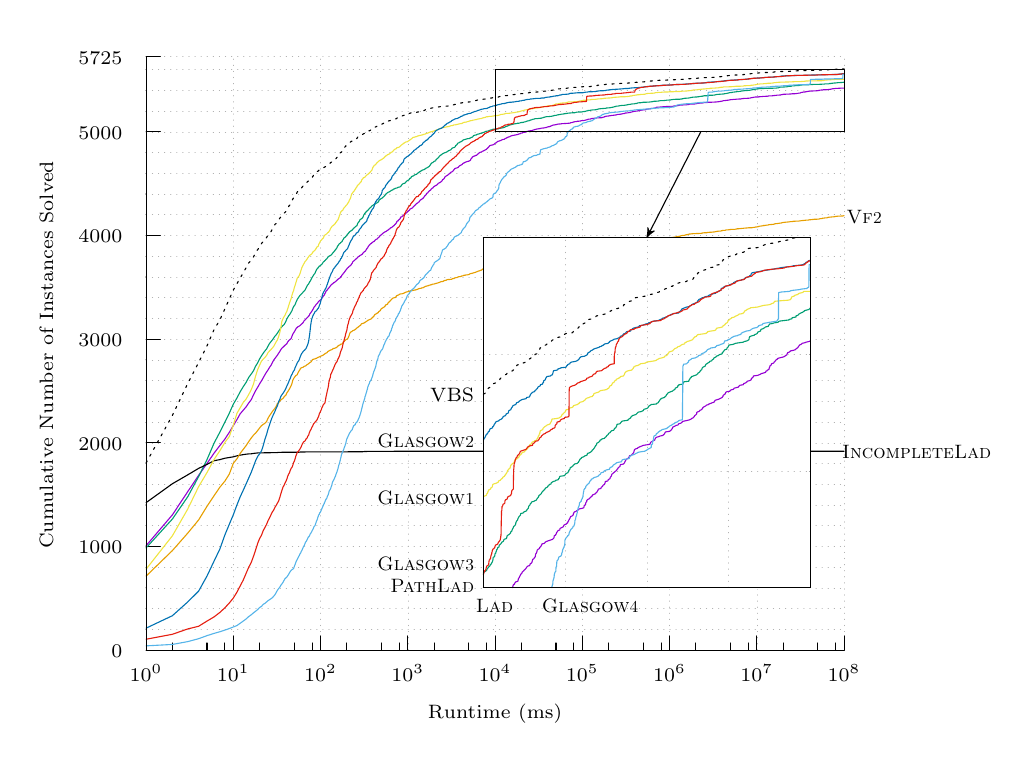
\begin{tikzpicture}[gnuplot]
%% generated with GNUPLOT 5.0p0 (Lua 5.2; terminal rev. 99, script rev. 100)
%% Wed 16 Dec 2015 16:57:53 GMT
\tikzset{every node/.append style={font={\scriptsize}}}
\path (0.000,0.000) rectangle (10.922,8.890);
\gpcolor{color=gp lt color axes}
\gpsetlinetype{gp lt axes}
\gpsetdashtype{gp dt axes}
\gpsetlinewidth{0.50}
\draw[gp path] (1.504,8.521)--(10.368,8.521);
\gpcolor{color=gp lt color border}
\gpsetlinetype{gp lt border}
\gpsetdashtype{gp dt solid}
\gpsetlinewidth{1.00}
\draw[gp path] (1.504,8.521)--(1.684,8.521);
\node[gp node right] at (1.320,8.521) {$5725$};
\gpcolor{color=gp lt color axes}
\gpsetlinetype{gp lt axes}
\gpsetdashtype{gp dt axes}
\gpsetlinewidth{0.50}
\draw[gp path] (1.504,0.985)--(10.368,0.985);
\gpcolor{color=gp lt color border}
\gpsetlinetype{gp lt border}
\gpsetdashtype{gp dt solid}
\gpsetlinewidth{1.00}
\draw[gp path] (1.504,0.985)--(1.684,0.985);
\node[gp node right] at (1.320,0.985) {$0$};
\gpcolor{color=gp lt color axes}
\gpsetlinetype{gp lt axes}
\gpsetdashtype{gp dt axes}
\gpsetlinewidth{0.50}
\draw[gp path] (1.504,1.248)--(10.368,1.248);
\gpcolor{color=gp lt color border}
\gpsetlinetype{gp lt border}
\gpsetdashtype{gp dt solid}
\gpsetlinewidth{1.00}
\draw[gp path] (1.504,1.248)--(1.505,1.248);
\gpcolor{color=gp lt color axes}
\gpsetlinetype{gp lt axes}
\gpsetdashtype{gp dt axes}
\gpsetlinewidth{0.50}
\draw[gp path] (1.504,1.512)--(10.368,1.512);
\gpcolor{color=gp lt color border}
\gpsetlinetype{gp lt border}
\gpsetdashtype{gp dt solid}
\gpsetlinewidth{1.00}
\draw[gp path] (1.504,1.512)--(1.505,1.512);
\gpcolor{color=gp lt color axes}
\gpsetlinetype{gp lt axes}
\gpsetdashtype{gp dt axes}
\gpsetlinewidth{0.50}
\draw[gp path] (1.504,1.775)--(10.368,1.775);
\gpcolor{color=gp lt color border}
\gpsetlinetype{gp lt border}
\gpsetdashtype{gp dt solid}
\gpsetlinewidth{1.00}
\draw[gp path] (1.504,1.775)--(1.505,1.775);
\gpcolor{color=gp lt color axes}
\gpsetlinetype{gp lt axes}
\gpsetdashtype{gp dt axes}
\gpsetlinewidth{0.50}
\draw[gp path] (1.504,2.038)--(10.368,2.038);
\gpcolor{color=gp lt color border}
\gpsetlinetype{gp lt border}
\gpsetdashtype{gp dt solid}
\gpsetlinewidth{1.00}
\draw[gp path] (1.504,2.038)--(1.505,2.038);
\gpcolor{color=gp lt color axes}
\gpsetlinetype{gp lt axes}
\gpsetdashtype{gp dt axes}
\gpsetlinewidth{0.50}
\draw[gp path] (1.504,2.301)--(10.368,2.301);
\gpcolor{color=gp lt color border}
\gpsetlinetype{gp lt border}
\gpsetdashtype{gp dt solid}
\gpsetlinewidth{1.00}
\draw[gp path] (1.504,2.301)--(1.684,2.301);
\node[gp node right] at (1.320,2.301) {$1000$};
\gpcolor{color=gp lt color axes}
\gpsetlinetype{gp lt axes}
\gpsetdashtype{gp dt axes}
\gpsetlinewidth{0.50}
\draw[gp path] (1.504,2.565)--(10.368,2.565);
\gpcolor{color=gp lt color border}
\gpsetlinetype{gp lt border}
\gpsetdashtype{gp dt solid}
\gpsetlinewidth{1.00}
\draw[gp path] (1.504,2.565)--(1.505,2.565);
\gpcolor{color=gp lt color axes}
\gpsetlinetype{gp lt axes}
\gpsetdashtype{gp dt axes}
\gpsetlinewidth{0.50}
\draw[gp path] (1.504,2.828)--(10.368,2.828);
\gpcolor{color=gp lt color border}
\gpsetlinetype{gp lt border}
\gpsetdashtype{gp dt solid}
\gpsetlinewidth{1.00}
\draw[gp path] (1.504,2.828)--(1.505,2.828);
\gpcolor{color=gp lt color axes}
\gpsetlinetype{gp lt axes}
\gpsetdashtype{gp dt axes}
\gpsetlinewidth{0.50}
\draw[gp path] (1.504,3.091)--(10.368,3.091);
\gpcolor{color=gp lt color border}
\gpsetlinetype{gp lt border}
\gpsetdashtype{gp dt solid}
\gpsetlinewidth{1.00}
\draw[gp path] (1.504,3.091)--(1.505,3.091);
\gpcolor{color=gp lt color axes}
\gpsetlinetype{gp lt axes}
\gpsetdashtype{gp dt axes}
\gpsetlinewidth{0.50}
\draw[gp path] (1.504,3.354)--(10.368,3.354);
\gpcolor{color=gp lt color border}
\gpsetlinetype{gp lt border}
\gpsetdashtype{gp dt solid}
\gpsetlinewidth{1.00}
\draw[gp path] (1.504,3.354)--(1.505,3.354);
\gpcolor{color=gp lt color axes}
\gpsetlinetype{gp lt axes}
\gpsetdashtype{gp dt axes}
\gpsetlinewidth{0.50}
\draw[gp path] (1.504,3.618)--(10.368,3.618);
\gpcolor{color=gp lt color border}
\gpsetlinetype{gp lt border}
\gpsetdashtype{gp dt solid}
\gpsetlinewidth{1.00}
\draw[gp path] (1.504,3.618)--(1.684,3.618);
\node[gp node right] at (1.320,3.618) {$2000$};
\gpcolor{color=gp lt color axes}
\gpsetlinetype{gp lt axes}
\gpsetdashtype{gp dt axes}
\gpsetlinewidth{0.50}
\draw[gp path] (1.504,3.881)--(10.368,3.881);
\gpcolor{color=gp lt color border}
\gpsetlinetype{gp lt border}
\gpsetdashtype{gp dt solid}
\gpsetlinewidth{1.00}
\draw[gp path] (1.504,3.881)--(1.505,3.881);
\gpcolor{color=gp lt color axes}
\gpsetlinetype{gp lt axes}
\gpsetdashtype{gp dt axes}
\gpsetlinewidth{0.50}
\draw[gp path] (1.504,4.144)--(10.368,4.144);
\gpcolor{color=gp lt color border}
\gpsetlinetype{gp lt border}
\gpsetdashtype{gp dt solid}
\gpsetlinewidth{1.00}
\draw[gp path] (1.504,4.144)--(1.505,4.144);
\gpcolor{color=gp lt color axes}
\gpsetlinetype{gp lt axes}
\gpsetdashtype{gp dt axes}
\gpsetlinewidth{0.50}
\draw[gp path] (1.504,4.407)--(10.368,4.407);
\gpcolor{color=gp lt color border}
\gpsetlinetype{gp lt border}
\gpsetdashtype{gp dt solid}
\gpsetlinewidth{1.00}
\draw[gp path] (1.504,4.407)--(1.505,4.407);
\gpcolor{color=gp lt color axes}
\gpsetlinetype{gp lt axes}
\gpsetdashtype{gp dt axes}
\gpsetlinewidth{0.50}
\draw[gp path] (1.504,4.671)--(10.368,4.671);
\gpcolor{color=gp lt color border}
\gpsetlinetype{gp lt border}
\gpsetdashtype{gp dt solid}
\gpsetlinewidth{1.00}
\draw[gp path] (1.504,4.671)--(1.505,4.671);
\gpcolor{color=gp lt color axes}
\gpsetlinetype{gp lt axes}
\gpsetdashtype{gp dt axes}
\gpsetlinewidth{0.50}
\draw[gp path] (1.504,4.934)--(10.368,4.934);
\gpcolor{color=gp lt color border}
\gpsetlinetype{gp lt border}
\gpsetdashtype{gp dt solid}
\gpsetlinewidth{1.00}
\draw[gp path] (1.504,4.934)--(1.684,4.934);
\node[gp node right] at (1.320,4.934) {$3000$};
\gpcolor{color=gp lt color axes}
\gpsetlinetype{gp lt axes}
\gpsetdashtype{gp dt axes}
\gpsetlinewidth{0.50}
\draw[gp path] (1.504,5.197)--(10.368,5.197);
\gpcolor{color=gp lt color border}
\gpsetlinetype{gp lt border}
\gpsetdashtype{gp dt solid}
\gpsetlinewidth{1.00}
\draw[gp path] (1.504,5.197)--(1.505,5.197);
\gpcolor{color=gp lt color axes}
\gpsetlinetype{gp lt axes}
\gpsetdashtype{gp dt axes}
\gpsetlinewidth{0.50}
\draw[gp path] (1.504,5.461)--(10.368,5.461);
\gpcolor{color=gp lt color border}
\gpsetlinetype{gp lt border}
\gpsetdashtype{gp dt solid}
\gpsetlinewidth{1.00}
\draw[gp path] (1.504,5.461)--(1.505,5.461);
\gpcolor{color=gp lt color axes}
\gpsetlinetype{gp lt axes}
\gpsetdashtype{gp dt axes}
\gpsetlinewidth{0.50}
\draw[gp path] (1.504,5.724)--(10.368,5.724);
\gpcolor{color=gp lt color border}
\gpsetlinetype{gp lt border}
\gpsetdashtype{gp dt solid}
\gpsetlinewidth{1.00}
\draw[gp path] (1.504,5.724)--(1.505,5.724);
\gpcolor{color=gp lt color axes}
\gpsetlinetype{gp lt axes}
\gpsetdashtype{gp dt axes}
\gpsetlinewidth{0.50}
\draw[gp path] (1.504,5.987)--(10.368,5.987);
\gpcolor{color=gp lt color border}
\gpsetlinetype{gp lt border}
\gpsetdashtype{gp dt solid}
\gpsetlinewidth{1.00}
\draw[gp path] (1.504,5.987)--(1.505,5.987);
\gpcolor{color=gp lt color axes}
\gpsetlinetype{gp lt axes}
\gpsetdashtype{gp dt axes}
\gpsetlinewidth{0.50}
\draw[gp path] (1.504,6.250)--(10.368,6.250);
\gpcolor{color=gp lt color border}
\gpsetlinetype{gp lt border}
\gpsetdashtype{gp dt solid}
\gpsetlinewidth{1.00}
\draw[gp path] (1.504,6.250)--(1.684,6.250);
\node[gp node right] at (1.320,6.250) {$4000$};
\gpcolor{color=gp lt color axes}
\gpsetlinetype{gp lt axes}
\gpsetdashtype{gp dt axes}
\gpsetlinewidth{0.50}
\draw[gp path] (1.504,6.514)--(10.368,6.514);
\gpcolor{color=gp lt color border}
\gpsetlinetype{gp lt border}
\gpsetdashtype{gp dt solid}
\gpsetlinewidth{1.00}
\draw[gp path] (1.504,6.514)--(1.505,6.514);
\gpcolor{color=gp lt color axes}
\gpsetlinetype{gp lt axes}
\gpsetdashtype{gp dt axes}
\gpsetlinewidth{0.50}
\draw[gp path] (1.504,6.777)--(10.368,6.777);
\gpcolor{color=gp lt color border}
\gpsetlinetype{gp lt border}
\gpsetdashtype{gp dt solid}
\gpsetlinewidth{1.00}
\draw[gp path] (1.504,6.777)--(1.505,6.777);
\gpcolor{color=gp lt color axes}
\gpsetlinetype{gp lt axes}
\gpsetdashtype{gp dt axes}
\gpsetlinewidth{0.50}
\draw[gp path] (1.504,7.040)--(10.368,7.040);
\gpcolor{color=gp lt color border}
\gpsetlinetype{gp lt border}
\gpsetdashtype{gp dt solid}
\gpsetlinewidth{1.00}
\draw[gp path] (1.504,7.040)--(1.505,7.040);
\gpcolor{color=gp lt color axes}
\gpsetlinetype{gp lt axes}
\gpsetdashtype{gp dt axes}
\gpsetlinewidth{0.50}
\draw[gp path] (1.504,7.303)--(10.368,7.303);
\gpcolor{color=gp lt color border}
\gpsetlinetype{gp lt border}
\gpsetdashtype{gp dt solid}
\gpsetlinewidth{1.00}
\draw[gp path] (1.504,7.303)--(1.505,7.303);
\gpcolor{color=gp lt color axes}
\gpsetlinetype{gp lt axes}
\gpsetdashtype{gp dt axes}
\gpsetlinewidth{0.50}
\draw[gp path] (1.504,7.567)--(10.368,7.567);
\gpcolor{color=gp lt color border}
\gpsetlinetype{gp lt border}
\gpsetdashtype{gp dt solid}
\gpsetlinewidth{1.00}
\draw[gp path] (1.504,7.567)--(1.684,7.567);
\node[gp node right] at (1.320,7.567) {$5000$};
\gpcolor{color=gp lt color axes}
\gpsetlinetype{gp lt axes}
\gpsetdashtype{gp dt axes}
\gpsetlinewidth{0.50}
\draw[gp path] (1.504,7.830)--(10.368,7.830);
\gpcolor{color=gp lt color border}
\gpsetlinetype{gp lt border}
\gpsetdashtype{gp dt solid}
\gpsetlinewidth{1.00}
\draw[gp path] (1.504,7.830)--(1.505,7.830);
\gpcolor{color=gp lt color axes}
\gpsetlinetype{gp lt axes}
\gpsetdashtype{gp dt axes}
\gpsetlinewidth{0.50}
\draw[gp path] (1.504,8.093)--(10.368,8.093);
\gpcolor{color=gp lt color border}
\gpsetlinetype{gp lt border}
\gpsetdashtype{gp dt solid}
\gpsetlinewidth{1.00}
\draw[gp path] (1.504,8.093)--(1.505,8.093);
\gpcolor{color=gp lt color axes}
\gpsetlinetype{gp lt axes}
\gpsetdashtype{gp dt axes}
\gpsetlinewidth{0.50}
\draw[gp path] (1.504,8.356)--(10.368,8.356);
\gpcolor{color=gp lt color border}
\gpsetlinetype{gp lt border}
\gpsetdashtype{gp dt solid}
\gpsetlinewidth{1.00}
\draw[gp path] (1.504,8.356)--(1.505,8.356);
\gpcolor{color=gp lt color axes}
\gpsetlinetype{gp lt axes}
\gpsetdashtype{gp dt axes}
\gpsetlinewidth{0.50}
\draw[gp path] (1.504,0.985)--(1.504,8.521);
\gpcolor{color=gp lt color border}
\gpsetlinetype{gp lt border}
\gpsetdashtype{gp dt solid}
\gpsetlinewidth{1.00}
\draw[gp path] (1.504,0.985)--(1.504,1.165);
\node[gp node center] at (1.504,0.677) {$10^{0}$};
\draw[gp path] (1.838,0.985)--(1.838,1.075);
\draw[gp path] (2.278,0.985)--(2.278,1.075);
\draw[gp path] (2.505,0.985)--(2.505,1.075);
\gpcolor{color=gp lt color axes}
\gpsetlinetype{gp lt axes}
\gpsetdashtype{gp dt axes}
\gpsetlinewidth{0.50}
\draw[gp path] (2.612,0.985)--(2.612,8.521);
\gpcolor{color=gp lt color border}
\gpsetlinetype{gp lt border}
\gpsetdashtype{gp dt solid}
\gpsetlinewidth{1.00}
\draw[gp path] (2.612,0.985)--(2.612,1.165);
\node[gp node center] at (2.612,0.677) {$10^{1}$};
\draw[gp path] (2.946,0.985)--(2.946,1.075);
\draw[gp path] (3.386,0.985)--(3.386,1.075);
\draw[gp path] (3.613,0.985)--(3.613,1.075);
\gpcolor{color=gp lt color axes}
\gpsetlinetype{gp lt axes}
\gpsetdashtype{gp dt axes}
\gpsetlinewidth{0.50}
\draw[gp path] (3.720,0.985)--(3.720,8.521);
\gpcolor{color=gp lt color border}
\gpsetlinetype{gp lt border}
\gpsetdashtype{gp dt solid}
\gpsetlinewidth{1.00}
\draw[gp path] (3.720,0.985)--(3.720,1.165);
\node[gp node center] at (3.720,0.677) {$10^{2}$};
\draw[gp path] (4.054,0.985)--(4.054,1.075);
\draw[gp path] (4.494,0.985)--(4.494,1.075);
\draw[gp path] (4.721,0.985)--(4.721,1.075);
\gpcolor{color=gp lt color axes}
\gpsetlinetype{gp lt axes}
\gpsetdashtype{gp dt axes}
\gpsetlinewidth{0.50}
\draw[gp path] (4.828,0.985)--(4.828,8.521);
\gpcolor{color=gp lt color border}
\gpsetlinetype{gp lt border}
\gpsetdashtype{gp dt solid}
\gpsetlinewidth{1.00}
\draw[gp path] (4.828,0.985)--(4.828,1.165);
\node[gp node center] at (4.828,0.677) {$10^{3}$};
\draw[gp path] (5.162,0.985)--(5.162,1.075);
\draw[gp path] (5.602,0.985)--(5.602,1.075);
\draw[gp path] (5.829,0.985)--(5.829,1.075);
\gpcolor{color=gp lt color axes}
\gpsetlinetype{gp lt axes}
\gpsetdashtype{gp dt axes}
\gpsetlinewidth{0.50}
\draw[gp path] (5.936,0.985)--(5.936,8.521);
\gpcolor{color=gp lt color border}
\gpsetlinetype{gp lt border}
\gpsetdashtype{gp dt solid}
\gpsetlinewidth{1.00}
\draw[gp path] (5.936,0.985)--(5.936,1.165);
\node[gp node center] at (5.936,0.677) {$10^{4}$};
\draw[gp path] (6.270,0.985)--(6.270,1.075);
\draw[gp path] (6.710,0.985)--(6.710,1.075);
\draw[gp path] (6.937,0.985)--(6.937,1.075);
\gpcolor{color=gp lt color axes}
\gpsetlinetype{gp lt axes}
\gpsetdashtype{gp dt axes}
\gpsetlinewidth{0.50}
\draw[gp path] (7.044,0.985)--(7.044,8.521);
\gpcolor{color=gp lt color border}
\gpsetlinetype{gp lt border}
\gpsetdashtype{gp dt solid}
\gpsetlinewidth{1.00}
\draw[gp path] (7.044,0.985)--(7.044,1.165);
\node[gp node center] at (7.044,0.677) {$10^{5}$};
\draw[gp path] (7.378,0.985)--(7.378,1.075);
\draw[gp path] (7.818,0.985)--(7.818,1.075);
\draw[gp path] (8.045,0.985)--(8.045,1.075);
\gpcolor{color=gp lt color axes}
\gpsetlinetype{gp lt axes}
\gpsetdashtype{gp dt axes}
\gpsetlinewidth{0.50}
\draw[gp path] (8.152,0.985)--(8.152,8.521);
\gpcolor{color=gp lt color border}
\gpsetlinetype{gp lt border}
\gpsetdashtype{gp dt solid}
\gpsetlinewidth{1.00}
\draw[gp path] (8.152,0.985)--(8.152,1.165);
\node[gp node center] at (8.152,0.677) {$10^{6}$};
\draw[gp path] (8.486,0.985)--(8.486,1.075);
\draw[gp path] (8.926,0.985)--(8.926,1.075);
\draw[gp path] (9.153,0.985)--(9.153,1.075);
\gpcolor{color=gp lt color axes}
\gpsetlinetype{gp lt axes}
\gpsetdashtype{gp dt axes}
\gpsetlinewidth{0.50}
\draw[gp path] (9.260,0.985)--(9.260,8.521);
\gpcolor{color=gp lt color border}
\gpsetlinetype{gp lt border}
\gpsetdashtype{gp dt solid}
\gpsetlinewidth{1.00}
\draw[gp path] (9.260,0.985)--(9.260,1.165);
\node[gp node center] at (9.260,0.677) {$10^{7}$};
\draw[gp path] (9.594,0.985)--(9.594,1.075);
\draw[gp path] (10.034,0.985)--(10.034,1.075);
\draw[gp path] (10.261,0.985)--(10.261,1.075);
\gpcolor{color=gp lt color axes}
\gpsetlinetype{gp lt axes}
\gpsetdashtype{gp dt axes}
\gpsetlinewidth{0.50}
\draw[gp path] (10.368,0.985)--(10.368,8.521);
\gpcolor{color=gp lt color border}
\gpsetlinetype{gp lt border}
\gpsetdashtype{gp dt solid}
\gpsetlinewidth{1.00}
\draw[gp path] (10.368,0.985)--(10.368,1.165);
\node[gp node center] at (10.368,0.677) {$10^{8}$};
\draw[gp path] (1.504,8.521)--(1.504,0.985)--(10.368,0.985);
\node[gp node center,rotate=-270] at (0.246,4.753) {Cumulative Number of Instances Solved};
\node[gp node center] at (5.936,0.215) {Runtime (ms)};
\gpcolor{rgb color={0.580,0.000,0.827}}
\draw[gp path] (1.504,2.311)--(1.838,2.703)--(2.033,2.998)--(2.171,3.204)--(2.278,3.356)%
  --(2.366,3.485)--(2.440,3.582)--(2.505,3.666)--(2.561,3.751)--(2.612,3.837)--(2.658,3.913)%
  --(2.700,3.988)--(2.738,4.032)--(2.774,4.074)--(2.807,4.123)--(2.838,4.164)--(2.867,4.224)%
  --(2.895,4.280)--(2.921,4.323)--(2.946,4.367)--(2.969,4.404)--(2.991,4.442)--(3.013,4.482)%
  --(3.033,4.515)--(3.053,4.544)--(3.072,4.576)--(3.090,4.602)--(3.107,4.634)--(3.124,4.667)%
  --(3.141,4.690)--(3.156,4.710)--(3.172,4.731)--(3.187,4.756)--(3.201,4.775)--(3.215,4.801)%
  --(3.228,4.819)--(3.242,4.831)--(3.254,4.843)--(3.267,4.856)--(3.279,4.866)--(3.291,4.876)%
  --(3.303,4.900)--(3.314,4.913)--(3.325,4.925)--(3.336,4.933)--(3.346,4.942)--(3.357,4.973)%
  --(3.367,4.997)--(3.377,5.013)--(3.386,5.027)--(3.396,5.045)--(3.405,5.062)--(3.414,5.076)%
  --(3.423,5.081)--(3.432,5.093)--(3.441,5.095)--(3.450,5.101)--(3.458,5.106)--(3.466,5.113)%
  --(3.474,5.122)--(3.482,5.129)--(3.490,5.135)--(3.498,5.145)--(3.505,5.156)--(3.513,5.172)%
  --(3.520,5.176)--(3.527,5.181)--(3.534,5.192)--(3.541,5.197)--(3.548,5.206)--(3.555,5.212)%
  --(3.562,5.220)--(3.569,5.228)--(3.575,5.233)--(3.582,5.251)--(3.588,5.262)--(3.594,5.268)%
  --(3.600,5.276)--(3.607,5.287)--(3.613,5.295)--(3.619,5.308)--(3.625,5.314)--(3.630,5.326)%
  --(3.636,5.338)--(3.642,5.346)--(3.647,5.351)--(3.653,5.359)--(3.658,5.367)--(3.664,5.374)%
  --(3.669,5.379)--(3.675,5.385)--(3.680,5.392)--(3.685,5.395)--(3.690,5.408)--(3.695,5.413)%
  --(3.700,5.417)--(3.705,5.420)--(3.710,5.426)--(3.715,5.429)--(3.720,5.433)--(3.725,5.436)%
  --(3.730,5.441)--(3.734,5.446)--(3.739,5.462)--(3.743,5.468)--(3.748,5.474)--(3.753,5.478)%
  --(3.757,5.484)--(3.761,5.487)--(3.766,5.493)--(3.770,5.501)--(3.775,5.516)--(3.779,5.518)%
  --(3.783,5.528)--(3.787,5.537)--(3.791,5.546)--(3.796,5.550)--(3.804,5.558)--(3.808,5.563)%
  --(3.812,5.570)--(3.816,5.576)--(3.820,5.578)--(3.824,5.582)--(3.827,5.588)--(3.831,5.595)%
  --(3.835,5.596)--(3.839,5.603)--(3.843,5.608)--(3.846,5.613)--(3.850,5.616)--(3.854,5.622)%
  --(3.857,5.629)--(3.861,5.630)--(3.864,5.633)--(3.868,5.634)--(3.871,5.637)--(3.875,5.638)%
  --(3.878,5.640)--(3.882,5.646)--(3.885,5.650)--(3.892,5.651)--(3.895,5.655)--(3.899,5.658)%
  --(3.905,5.661)--(3.909,5.666)--(3.915,5.669)--(3.918,5.672)--(3.921,5.676)--(3.925,5.680)%
  --(3.928,5.683)--(3.931,5.684)--(3.934,5.690)--(3.940,5.694)--(3.943,5.697)--(3.949,5.701)%
  --(3.952,5.703)--(3.955,5.704)--(3.958,5.707)--(3.961,5.708)--(3.964,5.711)--(3.967,5.712)%
  --(3.970,5.716)--(3.972,5.721)--(3.975,5.726)--(3.978,5.728)--(3.981,5.729)--(3.984,5.732)%
  --(3.987,5.737)--(3.989,5.744)--(3.992,5.749)--(3.995,5.751)--(4.000,5.754)--(4.003,5.761)%
  --(4.006,5.765)--(4.008,5.770)--(4.011,5.772)--(4.013,5.774)--(4.016,5.775)--(4.019,5.778)%
  --(4.021,5.783)--(4.024,5.786)--(4.026,5.791)--(4.029,5.794)--(4.031,5.798)--(4.034,5.800)%
  --(4.036,5.803)--(4.039,5.805)--(4.041,5.812)--(4.044,5.815)--(4.049,5.819)--(4.051,5.823)%
  --(4.054,5.826)--(4.056,5.832)--(4.058,5.834)--(4.061,5.836)--(4.063,5.838)--(4.068,5.841)%
  --(4.070,5.844)--(4.072,5.845)--(4.075,5.846)--(4.077,5.851)--(4.079,5.853)--(4.082,5.857)%
  --(4.084,5.858)--(4.086,5.861)--(4.091,5.862)--(4.093,5.865)--(4.095,5.866)--(4.097,5.867)%
  --(4.099,5.869)--(4.102,5.874)--(4.106,5.875)--(4.108,5.876)--(4.110,5.882)--(4.112,5.887)%
  --(4.114,5.890)--(4.119,5.894)--(4.121,5.899)--(4.123,5.903)--(4.125,5.907)--(4.127,5.912)%
  --(4.129,5.915)--(4.131,5.919)--(4.133,5.920)--(4.135,5.923)--(4.139,5.925)--(4.141,5.928)%
  --(4.145,5.929)--(4.147,5.932)--(4.149,5.934)--(4.155,5.940)--(4.157,5.941)--(4.159,5.944)%
  --(4.161,5.945)--(4.163,5.948)--(4.165,5.949)--(4.169,5.950)--(4.170,5.952)--(4.172,5.954)%
  --(4.174,5.957)--(4.176,5.958)--(4.180,5.962)--(4.183,5.963)--(4.185,5.966)--(4.187,5.967)%
  --(4.189,5.969)--(4.191,5.970)--(4.193,5.973)--(4.194,5.975)--(4.196,5.980)--(4.198,5.982)%
  --(4.200,5.983)--(4.207,5.986)--(4.210,5.988)--(4.212,5.991)--(4.214,5.992)--(4.215,5.994)%
  --(4.219,5.995)--(4.221,5.996)--(4.222,5.998)--(4.224,5.999)--(4.227,6.000)--(4.232,6.002)%
  --(4.234,6.003)--(4.236,6.005)--(4.239,6.007)--(4.241,6.009)--(4.242,6.011)--(4.245,6.012)%
  --(4.250,6.013)--(4.252,6.016)--(4.253,6.019)--(4.255,6.023)--(4.257,6.024)--(4.258,6.025)%
  --(4.260,6.027)--(4.261,6.031)--(4.263,6.032)--(4.264,6.033)--(4.266,6.037)--(4.271,6.038)%
  --(4.272,6.040)--(4.274,6.041)--(4.275,6.044)--(4.277,6.045)--(4.278,6.046)--(4.280,6.048)%
  --(4.283,6.050)--(4.289,6.052)--(4.292,6.056)--(4.293,6.057)--(4.295,6.058)--(4.296,6.065)%
  --(4.297,6.067)--(4.299,6.070)--(4.302,6.074)--(4.303,6.075)--(4.305,6.078)--(4.306,6.081)%
  --(4.307,6.083)--(4.309,6.086)--(4.310,6.088)--(4.312,6.090)--(4.315,6.091)--(4.316,6.092)%
  --(4.317,6.094)--(4.319,6.096)--(4.320,6.099)--(4.321,6.103)--(4.323,6.106)--(4.324,6.107)%
  --(4.326,6.111)--(4.327,6.112)--(4.328,6.115)--(4.331,6.119)--(4.332,6.120)--(4.334,6.121)%
  --(4.335,6.123)--(4.336,6.125)--(4.338,6.128)--(4.339,6.129)--(4.340,6.131)--(4.343,6.132)%
  --(4.346,6.134)--(4.347,6.138)--(4.348,6.140)--(4.351,6.141)--(4.353,6.142)--(4.355,6.144)%
  --(4.359,6.148)--(4.362,6.149)--(4.367,6.150)--(4.369,6.153)--(4.370,6.157)--(4.371,6.158)%
  --(4.372,6.160)--(4.375,6.161)--(4.379,6.162)--(4.381,6.165)--(4.382,6.167)--(4.387,6.169)%
  --(4.388,6.170)--(4.389,6.171)--(4.394,6.173)--(4.397,6.174)--(4.398,6.175)--(4.402,6.177)%
  --(4.404,6.181)--(4.405,6.182)--(4.406,6.183)--(4.407,6.185)--(4.409,6.187)--(4.411,6.188)%
  --(4.412,6.191)--(4.414,6.192)--(4.415,6.195)--(4.417,6.196)--(4.420,6.198)--(4.421,6.199)%
  --(4.423,6.200)--(4.430,6.203)--(4.432,6.204)--(4.437,6.206)--(4.441,6.208)--(4.443,6.211)%
  --(4.444,6.212)--(4.445,6.213)--(4.447,6.215)--(4.448,6.219)--(4.450,6.220)--(4.452,6.223)%
  --(4.453,6.224)--(4.454,6.225)--(4.459,6.228)--(4.460,6.229)--(4.463,6.231)--(4.465,6.232)%
  --(4.466,6.233)--(4.467,6.235)--(4.468,6.236)--(4.469,6.237)--(4.470,6.240)--(4.471,6.242)%
  --(4.472,6.245)--(4.473,6.246)--(4.475,6.249)--(4.481,6.250)--(4.482,6.252)--(4.483,6.254)%
  --(4.485,6.256)--(4.486,6.258)--(4.491,6.260)--(4.492,6.261)--(4.496,6.263)--(4.498,6.265)%
  --(4.499,6.266)--(4.501,6.267)--(4.502,6.269)--(4.503,6.270)--(4.504,6.271)--(4.505,6.273)%
  --(4.507,6.274)--(4.508,6.275)--(4.509,6.277)--(4.511,6.278)--(4.515,6.281)--(4.518,6.282)%
  --(4.519,6.283)--(4.523,6.287)--(4.527,6.289)--(4.529,6.290)--(4.530,6.291)--(4.531,6.294)%
  --(4.534,6.295)--(4.542,6.296)--(4.544,6.299)--(4.547,6.300)--(4.551,6.302)--(4.557,6.304)%
  --(4.558,6.307)--(4.560,6.308)--(4.561,6.310)--(4.563,6.311)--(4.564,6.312)--(4.567,6.314)%
  --(4.569,6.316)--(4.575,6.317)--(4.576,6.319)--(4.577,6.320)--(4.578,6.321)--(4.580,6.324)%
  --(4.581,6.325)--(4.582,6.327)--(4.586,6.328)--(4.587,6.329)--(4.590,6.331)--(4.592,6.332)%
  --(4.593,6.335)--(4.599,6.336)--(4.600,6.337)--(4.603,6.339)--(4.604,6.344)--(4.606,6.345)%
  --(4.606,6.346)--(4.609,6.348)--(4.611,6.349)--(4.620,6.350)--(4.621,6.352)--(4.623,6.353)%
  --(4.624,6.354)--(4.626,6.356)--(4.627,6.357)--(4.628,6.360)--(4.635,6.361)--(4.635,6.362)%
  --(4.636,6.365)--(4.637,6.366)--(4.639,6.367)--(4.641,6.369)--(4.642,6.370)--(4.644,6.371)%
  --(4.648,6.373)--(4.649,6.374)--(4.650,6.375)--(4.653,6.377)--(4.656,6.378)--(4.657,6.382)%
  --(4.658,6.385)--(4.658,6.386)--(4.660,6.387)--(4.661,6.389)--(4.663,6.390)--(4.664,6.391)%
  --(4.669,6.392)--(4.669,6.394)--(4.670,6.395)--(4.671,6.396)--(4.671,6.398)--(4.675,6.400)%
  --(4.677,6.402)--(4.677,6.404)--(4.678,6.406)--(4.679,6.407)--(4.679,6.408)--(4.682,6.410)%
  --(4.684,6.411)--(4.684,6.414)--(4.685,6.415)--(4.686,6.418)--(4.686,6.421)--(4.688,6.423)%
  --(4.690,6.424)--(4.691,6.428)--(4.691,6.432)--(4.693,6.433)--(4.693,6.435)--(4.704,6.436)%
  --(4.706,6.437)--(4.707,6.439)--(4.708,6.440)--(4.709,6.444)--(4.710,6.446)--(4.711,6.449)%
  --(4.713,6.450)--(4.719,6.452)--(4.720,6.453)--(4.721,6.454)--(4.722,6.456)--(4.723,6.457)%
  --(4.724,6.458)--(4.726,6.461)--(4.727,6.462)--(4.728,6.465)--(4.729,6.468)--(4.732,6.469)%
  --(4.733,6.470)--(4.733,6.471)--(4.734,6.474)--(4.735,6.477)--(4.737,6.481)--(4.738,6.483)%
  --(4.738,6.485)--(4.743,6.486)--(4.745,6.487)--(4.753,6.489)--(4.754,6.491)--(4.754,6.493)%
  --(4.757,6.496)--(4.762,6.498)--(4.763,6.500)--(4.764,6.502)--(4.766,6.503)--(4.767,6.504)%
  --(4.768,6.506)--(4.769,6.507)--(4.770,6.508)--(4.772,6.511)--(4.783,6.512)--(4.783,6.514)%
  --(4.784,6.515)--(4.789,6.516)--(4.789,6.518)--(4.790,6.519)--(4.792,6.520)--(4.794,6.521)%
  --(4.794,6.524)--(4.795,6.525)--(4.796,6.527)--(4.797,6.528)--(4.798,6.529)--(4.800,6.531)%
  --(4.801,6.532)--(4.804,6.533)--(4.807,6.536)--(4.809,6.537)--(4.810,6.539)--(4.812,6.540)%
  --(4.814,6.541)--(4.816,6.543)--(4.819,6.545)--(4.820,6.547)--(4.821,6.548)--(4.821,6.550)%
  --(4.822,6.552)--(4.823,6.553)--(4.823,6.554)--(4.826,6.556)--(4.827,6.557)--(4.829,6.558)%
  --(4.832,6.560)--(4.833,6.562)--(4.837,6.564)--(4.838,6.566)--(4.840,6.568)--(4.843,6.569)%
  --(4.848,6.570)--(4.849,6.572)--(4.850,6.573)--(4.851,6.574)--(4.851,6.577)--(4.851,6.578)%
  --(4.852,6.579)--(4.853,6.583)--(4.855,6.586)--(4.856,6.587)--(4.861,6.589)--(4.865,6.590)%
  --(4.868,6.591)--(4.869,6.593)--(4.869,6.594)--(4.873,6.595)--(4.876,6.597)--(4.882,6.598)%
  --(4.883,6.599)--(4.886,6.600)--(4.886,6.602)--(4.889,6.604)--(4.891,6.606)--(4.893,6.608)%
  --(4.893,6.610)--(4.894,6.611)--(4.896,6.612)--(4.897,6.614)--(4.897,6.615)--(4.901,6.616)%
  --(4.902,6.619)--(4.904,6.620)--(4.906,6.623)--(4.907,6.624)--(4.909,6.625)--(4.911,6.627)%
  --(4.913,6.629)--(4.913,6.631)--(4.914,6.632)--(4.915,6.633)--(4.917,6.635)--(4.921,6.636)%
  --(4.921,6.637)--(4.925,6.640)--(4.926,6.641)--(4.926,6.643)--(4.927,6.644)--(4.927,6.645)%
  --(4.928,6.647)--(4.931,6.648)--(4.932,6.649)--(4.933,6.650)--(4.938,6.652)--(4.939,6.653)%
  --(4.940,6.656)--(4.941,6.657)--(4.943,6.658)--(4.944,6.660)--(4.950,6.661)--(4.950,6.662)%
  --(4.954,6.665)--(4.955,6.666)--(4.955,6.668)--(4.958,6.669)--(4.958,6.670)--(4.960,6.672)%
  --(4.963,6.673)--(4.964,6.674)--(4.966,6.676)--(4.971,6.677)--(4.972,6.678)--(4.973,6.679)%
  --(4.973,6.681)--(4.974,6.682)--(4.976,6.685)--(4.976,6.686)--(4.977,6.689)--(4.979,6.690)%
  --(4.980,6.691)--(4.981,6.693)--(4.982,6.694)--(4.983,6.695)--(4.984,6.697)--(4.986,6.698)%
  --(4.986,6.699)--(4.987,6.701)--(4.989,6.702)--(4.991,6.703)--(4.994,6.704)--(4.996,6.706)%
  --(4.998,6.707)--(5.000,6.708)--(5.004,6.710)--(5.005,6.711)--(5.005,6.712)--(5.007,6.714)%
  --(5.011,6.716)--(5.012,6.718)--(5.016,6.719)--(5.019,6.720)--(5.019,6.722)--(5.020,6.723)%
  --(5.022,6.724)--(5.023,6.726)--(5.025,6.728)--(5.026,6.729)--(5.026,6.731)--(5.030,6.735)%
  --(5.031,6.736)--(5.032,6.737)--(5.034,6.740)--(5.036,6.743)--(5.037,6.744)--(5.039,6.745)%
  --(5.039,6.747)--(5.040,6.748)--(5.040,6.749)--(5.041,6.751)--(5.043,6.754)--(5.045,6.756)%
  --(5.048,6.757)--(5.049,6.758)--(5.051,6.760)--(5.053,6.761)--(5.054,6.762)--(5.054,6.764)%
  --(5.057,6.765)--(5.058,6.768)--(5.059,6.769)--(5.059,6.770)--(5.060,6.772)--(5.060,6.773)%
  --(5.061,6.774)--(5.064,6.776)--(5.064,6.777)--(5.065,6.778)--(5.065,6.779)--(5.066,6.781)%
  --(5.067,6.783)--(5.067,6.785)--(5.069,6.786)--(5.069,6.787)--(5.071,6.789)--(5.078,6.790)%
  --(5.082,6.791)--(5.082,6.794)--(5.083,6.797)--(5.084,6.798)--(5.085,6.799)--(5.087,6.801)%
  --(5.087,6.802)--(5.088,6.803)--(5.088,6.805)--(5.088,6.806)--(5.090,6.807)--(5.092,6.808)%
  --(5.093,6.811)--(5.097,6.812)--(5.098,6.814)--(5.100,6.815)--(5.102,6.816)--(5.103,6.818)%
  --(5.103,6.819)--(5.104,6.820)--(5.106,6.822)--(5.106,6.823)--(5.111,6.824)--(5.115,6.826)%
  --(5.116,6.827)--(5.117,6.828)--(5.117,6.830)--(5.119,6.831)--(5.121,6.832)--(5.121,6.836)%
  --(5.122,6.837)--(5.122,6.839)--(5.125,6.840)--(5.130,6.843)--(5.131,6.844)--(5.131,6.845)%
  --(5.132,6.847)--(5.134,6.848)--(5.134,6.849)--(5.136,6.852)--(5.146,6.853)--(5.146,6.855)%
  --(5.147,6.857)--(5.147,6.858)--(5.148,6.860)--(5.149,6.861)--(5.149,6.862)--(5.154,6.864)%
  --(5.155,6.865)--(5.156,6.866)--(5.156,6.870)--(5.163,6.873)--(5.165,6.874)--(5.166,6.876)%
  --(5.168,6.877)--(5.171,6.880)--(5.174,6.881)--(5.177,6.882)--(5.178,6.883)--(5.181,6.885)%
  --(5.186,6.886)--(5.187,6.887)--(5.189,6.889)--(5.189,6.890)--(5.192,6.891)--(5.194,6.893)%
  --(5.197,6.894)--(5.199,6.895)--(5.201,6.897)--(5.203,6.898)--(5.204,6.899)--(5.206,6.901)%
  --(5.206,6.902)--(5.208,6.903)--(5.210,6.906)--(5.210,6.907)--(5.211,6.908)--(5.211,6.910)%
  --(5.214,6.912)--(5.217,6.915)--(5.225,6.916)--(5.226,6.918)--(5.226,6.919)--(5.227,6.920)%
  --(5.232,6.922)--(5.236,6.923)--(5.239,6.924)--(5.239,6.926)--(5.240,6.927)--(5.241,6.928)%
  --(5.245,6.930)--(5.246,6.931)--(5.250,6.932)--(5.251,6.935)--(5.251,6.936)--(5.255,6.937)%
  --(5.255,6.939)--(5.259,6.941)--(5.260,6.943)--(5.261,6.944)--(5.262,6.945)--(5.263,6.947)%
  --(5.263,6.948)--(5.264,6.949)--(5.265,6.952)--(5.265,6.953)--(5.267,6.955)--(5.268,6.956)%
  --(5.268,6.957)--(5.269,6.959)--(5.270,6.960)--(5.275,6.962)--(5.277,6.964)--(5.278,6.965)%
  --(5.281,6.966)--(5.282,6.968)--(5.283,6.969)--(5.284,6.970)--(5.286,6.972)--(5.289,6.973)%
  --(5.290,6.974)--(5.291,6.976)--(5.292,6.977)--(5.292,6.978)--(5.293,6.981)--(5.294,6.982)%
  --(5.294,6.984)--(5.294,6.985)--(5.294,6.986)--(5.296,6.987)--(5.297,6.989)--(5.298,6.990)%
  --(5.299,6.993)--(5.300,6.994)--(5.301,6.995)--(5.302,6.997)--(5.305,6.998)--(5.306,6.999)%
  --(5.308,7.001)--(5.310,7.002)--(5.312,7.003)--(5.312,7.005)--(5.314,7.006)--(5.315,7.007)%
  --(5.318,7.009)--(5.323,7.010)--(5.326,7.011)--(5.327,7.012)--(5.329,7.014)--(5.331,7.015)%
  --(5.332,7.016)--(5.333,7.018)--(5.338,7.019)--(5.338,7.020)--(5.339,7.022)--(5.340,7.023)%
  --(5.341,7.024)--(5.341,7.026)--(5.347,7.027)--(5.347,7.028)--(5.350,7.030)--(5.352,7.031)%
  --(5.352,7.032)--(5.353,7.034)--(5.353,7.035)--(5.354,7.036)--(5.355,7.037)--(5.361,7.039)%
  --(5.361,7.040)--(5.363,7.041)--(5.365,7.043)--(5.366,7.044)--(5.368,7.047)--(5.369,7.049)%
  --(5.372,7.052)--(5.374,7.053)--(5.378,7.055)--(5.379,7.056)--(5.384,7.057)--(5.385,7.059)%
  --(5.389,7.060)--(5.392,7.061)--(5.392,7.063)--(5.393,7.064)--(5.396,7.065)--(5.399,7.066)%
  --(5.400,7.068)--(5.400,7.069)--(5.402,7.070)--(5.403,7.072)--(5.404,7.073)--(5.405,7.074)%
  --(5.405,7.076)--(5.409,7.078)--(5.409,7.080)--(5.410,7.081)--(5.411,7.082)--(5.412,7.084)%
  --(5.413,7.085)--(5.414,7.086)--(5.416,7.088)--(5.416,7.089)--(5.417,7.090)--(5.418,7.091)%
  --(5.419,7.093)--(5.420,7.094)--(5.421,7.095)--(5.422,7.097)--(5.424,7.098)--(5.424,7.099)%
  --(5.426,7.101)--(5.432,7.102)--(5.435,7.103)--(5.436,7.105)--(5.439,7.106)--(5.450,7.107)%
  --(5.451,7.109)--(5.451,7.110)--(5.454,7.111)--(5.460,7.113)--(5.464,7.114)--(5.464,7.115)%
  --(5.468,7.116)--(5.470,7.118)--(5.471,7.119)--(5.471,7.120)--(5.471,7.122)--(5.473,7.123)%
  --(5.474,7.124)--(5.475,7.126)--(5.478,7.127)--(5.478,7.128)--(5.478,7.130)--(5.478,7.131)%
  --(5.481,7.132)--(5.482,7.134)--(5.484,7.135)--(5.485,7.136)--(5.489,7.138)--(5.491,7.139)%
  --(5.496,7.140)--(5.497,7.141)--(5.497,7.143)--(5.497,7.144)--(5.505,7.145)--(5.506,7.147)%
  --(5.511,7.148)--(5.512,7.149)--(5.512,7.151)--(5.517,7.152)--(5.518,7.153)--(5.519,7.155)%
  --(5.521,7.157)--(5.522,7.159)--(5.523,7.160)--(5.524,7.161)--(5.525,7.163)--(5.528,7.164)%
  --(5.528,7.166)--(5.533,7.168)--(5.533,7.169)--(5.541,7.170)--(5.543,7.172)--(5.544,7.173)%
  --(5.544,7.174)--(5.545,7.176)--(5.548,7.177)--(5.551,7.178)--(5.558,7.180)--(5.560,7.181)%
  --(5.561,7.182)--(5.565,7.184)--(5.568,7.185)--(5.572,7.186)--(5.577,7.188)--(5.581,7.189)%
  --(5.584,7.190)--(5.592,7.192)--(5.596,7.193)--(5.601,7.194)--(5.602,7.195)--(5.607,7.197)%
  --(5.610,7.198)--(5.613,7.199)--(5.614,7.201)--(5.618,7.202)--(5.619,7.203)--(5.621,7.205)%
  --(5.623,7.206)--(5.623,7.207)--(5.624,7.209)--(5.624,7.210)--(5.626,7.211)--(5.626,7.214)%
  --(5.626,7.215)--(5.627,7.217)--(5.627,7.218)--(5.627,7.219)--(5.628,7.220)--(5.629,7.222)%
  --(5.629,7.223)--(5.629,7.224)--(5.632,7.226)--(5.633,7.227)--(5.634,7.228)--(5.635,7.230)%
  --(5.636,7.231)--(5.638,7.232)--(5.639,7.234)--(5.639,7.235)--(5.642,7.236)--(5.643,7.238)%
  --(5.643,7.239)--(5.644,7.240)--(5.644,7.242)--(5.645,7.243)--(5.646,7.244)--(5.647,7.245)%
  --(5.647,7.247)--(5.651,7.248)--(5.653,7.249)--(5.655,7.251)--(5.656,7.252)--(5.657,7.253)%
  --(5.662,7.255)--(5.665,7.256)--(5.666,7.257)--(5.667,7.259)--(5.671,7.260)--(5.680,7.261)%
  --(5.685,7.263)--(5.686,7.264)--(5.687,7.267)--(5.692,7.268)--(5.694,7.269)--(5.703,7.270)%
  --(5.704,7.272)--(5.707,7.273)--(5.707,7.274)--(5.708,7.276)--(5.708,7.277)--(5.710,7.278)%
  --(5.710,7.280)--(5.714,7.281)--(5.715,7.282)--(5.716,7.284)--(5.719,7.285)--(5.720,7.286)%
  --(5.721,7.288)--(5.721,7.289)--(5.722,7.290)--(5.722,7.292)--(5.728,7.293)--(5.729,7.294)%
  --(5.731,7.295)--(5.732,7.297)--(5.733,7.298)--(5.734,7.299)--(5.735,7.301)--(5.735,7.302)%
  --(5.737,7.303)--(5.738,7.305)--(5.738,7.306)--(5.748,7.307)--(5.752,7.309)--(5.759,7.310)%
  --(5.761,7.311)--(5.763,7.313)--(5.768,7.314)--(5.770,7.315)--(5.770,7.317)--(5.771,7.318)%
  --(5.774,7.319)--(5.777,7.321)--(5.779,7.322)--(5.783,7.323)--(5.787,7.324)--(5.790,7.326)%
  --(5.790,7.327)--(5.799,7.328)--(5.800,7.330)--(5.802,7.331)--(5.803,7.332)--(5.805,7.334)%
  --(5.808,7.335)--(5.810,7.336)--(5.811,7.338)--(5.814,7.339)--(5.815,7.340)--(5.818,7.342)%
  --(5.824,7.343)--(5.825,7.344)--(5.826,7.346)--(5.826,7.347)--(5.828,7.348)--(5.828,7.349)%
  --(5.829,7.351)--(5.829,7.352)--(5.836,7.353)--(5.838,7.355)--(5.838,7.356)--(5.839,7.357)%
  --(5.839,7.359)--(5.841,7.360)--(5.841,7.361)--(5.844,7.363)--(5.845,7.364)--(5.846,7.365)%
  --(5.850,7.367)--(5.850,7.368)--(5.850,7.369)--(5.852,7.371)--(5.852,7.372)--(5.855,7.373)%
  --(5.856,7.374)--(5.856,7.376)--(5.857,7.377)--(5.858,7.378)--(5.860,7.380)--(5.862,7.381)%
  --(5.862,7.382)--(5.863,7.384)--(5.863,7.385)--(5.864,7.386)--(5.866,7.388)--(5.867,7.389)%
  --(5.868,7.390)--(5.869,7.392)--(5.874,7.393)--(5.875,7.394)--(5.884,7.396)--(5.887,7.397)%
  --(5.892,7.398)--(5.896,7.399)--(5.905,7.401)--(5.905,7.402)--(5.912,7.403)--(5.916,7.405)%
  --(5.919,7.406)--(5.920,7.407)--(5.924,7.409)--(5.925,7.410)--(5.927,7.411)--(5.928,7.413)%
  --(5.929,7.414)--(5.931,7.415)--(5.932,7.417)--(5.933,7.418)--(5.933,7.419)--(5.936,7.421)%
  --(5.937,7.422)--(5.937,7.423)--(5.940,7.424)--(5.942,7.426)--(5.952,7.428)--(5.952,7.430)%
  --(5.953,7.431)--(5.954,7.432)--(5.954,7.434)--(5.958,7.435)--(5.960,7.436)--(5.961,7.438)%
  --(5.962,7.439)--(5.966,7.440)--(5.966,7.442)--(5.968,7.443)--(5.968,7.444)--(5.970,7.446)%
  --(5.974,7.447)--(5.979,7.448)--(5.988,7.450)--(5.991,7.451)--(5.994,7.452)--(5.995,7.453)%
  --(5.996,7.455)--(6.004,7.456)--(6.009,7.457)--(6.012,7.459)--(6.013,7.460)--(6.016,7.461)%
  --(6.017,7.463)--(6.020,7.464)--(6.021,7.465)--(6.025,7.467)--(6.027,7.468)--(6.036,7.469)%
  --(6.038,7.471)--(6.050,7.472)--(6.054,7.473)--(6.057,7.475)--(6.058,7.476)--(6.059,7.477)%
  --(6.059,7.478)--(6.061,7.480)--(6.065,7.481)--(6.066,7.482)--(6.074,7.484)--(6.074,7.485)%
  --(6.078,7.486)--(6.079,7.488)--(6.081,7.489)--(6.085,7.490)--(6.088,7.492)--(6.089,7.493)%
  --(6.089,7.494)--(6.091,7.496)--(6.092,7.497)--(6.099,7.498)--(6.101,7.500)--(6.105,7.501)%
  --(6.111,7.502)--(6.118,7.503)--(6.120,7.505)--(6.123,7.506)--(6.125,7.507)--(6.128,7.509)%
  --(6.130,7.510)--(6.131,7.511)--(6.134,7.513)--(6.135,7.514)--(6.141,7.515)--(6.146,7.517)%
  --(6.146,7.518)--(6.152,7.519)--(6.159,7.521)--(6.168,7.522)--(6.175,7.523)--(6.181,7.525)%
  --(6.182,7.526)--(6.189,7.527)--(6.203,7.528)--(6.204,7.530)--(6.209,7.531)--(6.219,7.532)%
  --(6.222,7.534)--(6.223,7.535)--(6.231,7.536)--(6.238,7.538)--(6.238,7.539)--(6.240,7.540)%
  --(6.250,7.542)--(6.254,7.543)--(6.254,7.544)--(6.258,7.546)--(6.260,7.547)--(6.260,7.548)%
  --(6.262,7.550)--(6.268,7.551)--(6.281,7.552)--(6.281,7.553)--(6.282,7.555)--(6.288,7.556)%
  --(6.288,7.557)--(6.291,7.559)--(6.301,7.560)--(6.317,7.561)--(6.318,7.563)--(6.326,7.564)%
  --(6.330,7.565)--(6.333,7.567)--(6.334,7.568)--(6.335,7.569)--(6.336,7.571)--(6.340,7.572)%
  --(6.343,7.573)--(6.357,7.575)--(6.358,7.576)--(6.361,7.577)--(6.370,7.579)--(6.374,7.580)%
  --(6.402,7.581)--(6.405,7.582)--(6.407,7.584)--(6.408,7.585)--(6.410,7.586)--(6.412,7.588)%
  --(6.422,7.589)--(6.423,7.590)--(6.426,7.592)--(6.432,7.593)--(6.436,7.594)--(6.438,7.596)%
  --(6.445,7.597)--(6.448,7.598)--(6.459,7.600)--(6.461,7.601)--(6.464,7.602)--(6.472,7.604)%
  --(6.484,7.605)--(6.488,7.606)--(6.500,7.607)--(6.504,7.609)--(6.514,7.610)--(6.518,7.611)%
  --(6.521,7.613)--(6.529,7.614)--(6.539,7.615)--(6.563,7.617)--(6.565,7.618)--(6.570,7.619)%
  --(6.571,7.621)--(6.585,7.622)--(6.590,7.623)--(6.595,7.625)--(6.596,7.626)--(6.599,7.627)%
  --(6.602,7.629)--(6.604,7.630)--(6.610,7.631)--(6.624,7.632)--(6.625,7.634)--(6.633,7.635)%
  --(6.639,7.636)--(6.640,7.638)--(6.640,7.639)--(6.643,7.640)--(6.644,7.642)--(6.645,7.643)%
  --(6.654,7.644)--(6.656,7.646)--(6.660,7.647)--(6.663,7.648)--(6.664,7.650)--(6.664,7.651)%
  --(6.670,7.652)--(6.680,7.654)--(6.695,7.655)--(6.698,7.656)--(6.699,7.657)--(6.710,7.659)%
  --(6.713,7.660)--(6.723,7.661)--(6.724,7.663)--(6.729,7.664)--(6.730,7.665)--(6.764,7.667)%
  --(6.768,7.668)--(6.775,7.669)--(6.786,7.671)--(6.809,7.672)--(6.832,7.673)--(6.853,7.675)%
  --(6.876,7.676)--(6.882,7.677)--(6.891,7.679)--(6.894,7.680)--(6.894,7.681)--(6.896,7.682)%
  --(6.897,7.684)--(6.913,7.685)--(6.914,7.686)--(6.923,7.688)--(6.926,7.689)--(6.927,7.690)%
  --(6.931,7.692)--(6.943,7.693)--(6.944,7.694)--(6.947,7.696)--(6.973,7.697)--(6.973,7.698)%
  --(6.974,7.700)--(6.980,7.701)--(6.997,7.702)--(7.015,7.704)--(7.023,7.705)--(7.025,7.706)%
  --(7.028,7.708)--(7.037,7.709)--(7.061,7.710)--(7.061,7.711)--(7.079,7.713)--(7.080,7.714)%
  --(7.081,7.715)--(7.089,7.717)--(7.091,7.718)--(7.095,7.719)--(7.103,7.721)--(7.104,7.722)%
  --(7.110,7.723)--(7.112,7.725)--(7.115,7.726)--(7.119,7.727)--(7.139,7.729)--(7.149,7.730)%
  --(7.154,7.731)--(7.155,7.733)--(7.157,7.734)--(7.163,7.735)--(7.164,7.736)--(7.172,7.738)%
  --(7.193,7.739)--(7.201,7.740)--(7.218,7.742)--(7.226,7.743)--(7.234,7.744)--(7.272,7.746)%
  --(7.298,7.747)--(7.298,7.748)--(7.302,7.750)--(7.303,7.751)--(7.304,7.752)--(7.320,7.754)%
  --(7.321,7.755)--(7.322,7.756)--(7.323,7.758)--(7.327,7.759)--(7.333,7.760)--(7.337,7.761)%
  --(7.338,7.763)--(7.341,7.764)--(7.346,7.765)--(7.365,7.767)--(7.376,7.768)--(7.381,7.769)%
  --(7.389,7.771)--(7.399,7.772)--(7.408,7.773)--(7.415,7.775)--(7.416,7.776)--(7.436,7.777)%
  --(7.453,7.779)--(7.457,7.780)--(7.470,7.781)--(7.476,7.783)--(7.478,7.784)--(7.486,7.785)%
  --(7.491,7.786)--(7.491,7.788)--(7.496,7.789)--(7.528,7.790)--(7.532,7.792)--(7.533,7.793)%
  --(7.545,7.794)--(7.553,7.796)--(7.556,7.797)--(7.562,7.798)--(7.579,7.800)--(7.581,7.801)%
  --(7.584,7.802)--(7.587,7.804)--(7.588,7.805)--(7.590,7.806)--(7.623,7.808)--(7.627,7.809)%
  --(7.628,7.810)--(7.639,7.811)--(7.654,7.813)--(7.655,7.814)--(7.655,7.815)--(7.662,7.817)%
  --(7.670,7.818)--(7.672,7.819)--(7.676,7.821)--(7.677,7.822)--(7.683,7.823)--(7.695,7.825)%
  --(7.699,7.826)--(7.714,7.827)--(7.719,7.829)--(7.731,7.830)--(7.741,7.831)--(7.747,7.833)%
  --(7.748,7.834)--(7.761,7.835)--(7.762,7.837)--(7.765,7.838)--(7.780,7.839)--(7.789,7.840)%
  --(7.790,7.842)--(7.791,7.843)--(7.796,7.844)--(7.836,7.846)--(7.843,7.847)--(7.851,7.848)%
  --(7.852,7.850)--(7.856,7.851)--(7.861,7.852)--(7.864,7.854)--(7.868,7.855)--(7.874,7.856)%
  --(7.887,7.858)--(7.901,7.859)--(7.909,7.860)--(7.912,7.862)--(7.914,7.863)--(7.915,7.864)%
  --(7.943,7.865)--(7.949,7.867)--(7.954,7.868)--(7.962,7.869)--(7.971,7.871)--(7.976,7.872)%
  --(7.978,7.873)--(7.979,7.875)--(7.983,7.876)--(7.983,7.877)--(7.987,7.879)--(8.002,7.880)%
  --(8.027,7.881)--(8.032,7.883)--(8.049,7.884)--(8.064,7.885)--(8.086,7.887)--(8.101,7.888)%
  --(8.157,7.889)--(8.196,7.890)--(8.197,7.892)--(8.201,7.893)--(8.203,7.894)--(8.213,7.896)%
  --(8.229,7.897)--(8.239,7.898)--(8.260,7.900)--(8.261,7.901)--(8.265,7.902)--(8.269,7.904)%
  --(8.274,7.905)--(8.286,7.906)--(8.315,7.908)--(8.332,7.909)--(8.370,7.910)--(8.376,7.912)%
  --(8.387,7.913)--(8.392,7.914)--(8.395,7.915)--(8.403,7.917)--(8.405,7.918)--(8.461,7.919)%
  --(8.470,7.921)--(8.480,7.922)--(8.489,7.923)--(8.491,7.925)--(8.499,7.926)--(8.501,7.927)%
  --(8.502,7.929)--(8.517,7.930)--(8.536,7.931)--(8.546,7.933)--(8.575,7.934)--(8.581,7.935)%
  --(8.584,7.937)--(8.614,7.938)--(8.622,7.939)--(8.634,7.940)--(8.634,7.942)--(8.672,7.943)%
  --(8.710,7.944)--(8.735,7.946)--(8.754,7.947)--(8.759,7.948)--(8.776,7.950)--(8.785,7.951)%
  --(8.792,7.952)--(8.800,7.954)--(8.801,7.955)--(8.813,7.956)--(8.823,7.958)--(8.828,7.959)%
  --(8.829,7.960)--(8.830,7.962)--(8.834,7.963)--(8.856,7.964)--(8.868,7.966)--(8.871,7.967)%
  --(8.892,7.968)--(8.897,7.969)--(8.909,7.971)--(8.910,7.972)--(8.915,7.973)--(8.925,7.975)%
  --(8.942,7.976)--(8.954,7.977)--(8.960,7.979)--(8.993,7.980)--(8.993,7.981)--(9.024,7.983)%
  --(9.036,7.984)--(9.065,7.985)--(9.067,7.987)--(9.075,7.988)--(9.076,7.989)--(9.097,7.991)%
  --(9.124,7.992)--(9.142,7.993)--(9.158,7.994)--(9.175,7.996)--(9.177,7.997)--(9.186,7.998)%
  --(9.187,8.000)--(9.192,8.001)--(9.204,8.002)--(9.213,8.004)--(9.217,8.005)--(9.222,8.006)%
  --(9.224,8.008)--(9.242,8.009)--(9.283,8.010)--(9.283,8.012)--(9.292,8.013)--(9.325,8.014)%
  --(9.333,8.016)--(9.336,8.017)--(9.364,8.018)--(9.397,8.019)--(9.398,8.021)--(9.409,8.022)%
  --(9.414,8.023)--(9.463,8.025)--(9.464,8.026)--(9.467,8.027)--(9.492,8.029)--(9.501,8.030)%
  --(9.512,8.031)--(9.514,8.033)--(9.545,8.034)--(9.564,8.035)--(9.569,8.037)--(9.570,8.038)%
  --(9.572,8.039)--(9.587,8.041)--(9.593,8.042)--(9.597,8.043)--(9.598,8.044)--(9.656,8.046)%
  --(9.675,8.047)--(9.694,8.048)--(9.704,8.050)--(9.735,8.051)--(9.760,8.052)--(9.766,8.054)%
  --(9.768,8.055)--(9.784,8.056)--(9.788,8.058)--(9.809,8.059)--(9.811,8.060)--(9.811,8.062)%
  --(9.814,8.063)--(9.817,8.064)--(9.821,8.066)--(9.821,8.067)--(9.833,8.068)--(9.840,8.069)%
  --(9.842,8.071)--(9.844,8.072)--(9.874,8.073)--(9.878,8.075)--(9.881,8.076)--(9.893,8.077)%
  --(9.895,8.079)--(9.905,8.080)--(9.907,8.081)--(9.927,8.083)--(9.927,8.084)--(9.951,8.085)%
  --(9.989,8.087)--(10.012,8.088)--(10.027,8.089)--(10.033,8.091)--(10.052,8.092)--(10.052,8.093)%
  --(10.057,8.095)--(10.061,8.096)--(10.063,8.097)--(10.086,8.098)--(10.096,8.100)--(10.103,8.101)%
  --(10.144,8.102)--(10.167,8.104)--(10.175,8.105)--(10.180,8.106)--(10.195,8.108)--(10.204,8.109)%
  --(10.207,8.110)--(10.212,8.112)--(10.221,8.113)--(10.222,8.114)--(10.244,8.116)--(10.254,8.117)%
  --(10.257,8.118)--(10.298,8.120)--(10.313,8.121)--(10.352,8.122)--(10.368,8.123);
\gpcolor{rgb color={0.000,0.620,0.451}}
\draw[gp path] (1.504,2.283)--(1.838,2.650)--(2.033,2.933)--(2.171,3.189)--(2.278,3.406)%
  --(2.366,3.611)--(2.440,3.752)--(2.505,3.881)--(2.561,3.995)--(2.612,4.109)--(2.658,4.188)%
  --(2.700,4.268)--(2.738,4.331)--(2.774,4.385)--(2.807,4.448)--(2.838,4.490)--(2.867,4.531)%
  --(2.895,4.592)--(2.921,4.633)--(2.946,4.684)--(2.969,4.722)--(2.991,4.755)--(3.013,4.785)%
  --(3.033,4.808)--(3.053,4.846)--(3.072,4.880)--(3.090,4.902)--(3.107,4.923)--(3.124,4.948)%
  --(3.141,4.973)--(3.156,4.989)--(3.172,5.012)--(3.187,5.034)--(3.201,5.056)--(3.215,5.077)%
  --(3.228,5.092)--(3.242,5.108)--(3.254,5.116)--(3.267,5.137)--(3.279,5.158)--(3.291,5.191)%
  --(3.303,5.210)--(3.314,5.230)--(3.325,5.243)--(3.336,5.260)--(3.346,5.278)--(3.357,5.297)%
  --(3.367,5.325)--(3.377,5.347)--(3.386,5.359)--(3.396,5.372)--(3.405,5.397)--(3.414,5.416)%
  --(3.423,5.437)--(3.432,5.451)--(3.441,5.466)--(3.450,5.478)--(3.458,5.491)--(3.466,5.496)%
  --(3.474,5.507)--(3.482,5.513)--(3.490,5.522)--(3.498,5.532)--(3.505,5.541)--(3.513,5.546)%
  --(3.520,5.555)--(3.527,5.565)--(3.534,5.580)--(3.541,5.596)--(3.548,5.609)--(3.555,5.622)%
  --(3.562,5.628)--(3.569,5.638)--(3.575,5.650)--(3.582,5.663)--(3.588,5.670)--(3.594,5.683)%
  --(3.600,5.694)--(3.607,5.708)--(3.613,5.719)--(3.619,5.728)--(3.625,5.738)--(3.630,5.746)%
  --(3.636,5.757)--(3.642,5.762)--(3.647,5.769)--(3.653,5.782)--(3.658,5.795)--(3.664,5.805)%
  --(3.669,5.819)--(3.675,5.824)--(3.680,5.836)--(3.685,5.838)--(3.690,5.840)--(3.695,5.849)%
  --(3.700,5.857)--(3.705,5.862)--(3.710,5.865)--(3.715,5.866)--(3.720,5.874)--(3.725,5.878)%
  --(3.730,5.879)--(3.734,5.884)--(3.739,5.888)--(3.743,5.896)--(3.748,5.903)--(3.753,5.912)%
  --(3.757,5.917)--(3.761,5.919)--(3.766,5.921)--(3.770,5.929)--(3.775,5.932)--(3.779,5.934)%
  --(3.783,5.940)--(3.787,5.946)--(3.791,5.949)--(3.796,5.952)--(3.800,5.957)--(3.804,5.963)%
  --(3.808,5.967)--(3.812,5.975)--(3.816,5.979)--(3.820,5.983)--(3.824,5.986)--(3.827,5.988)%
  --(3.831,5.990)--(3.839,5.994)--(3.846,5.996)--(3.850,6.000)--(3.854,6.005)--(3.857,6.007)%
  --(3.861,6.011)--(3.864,6.013)--(3.868,6.020)--(3.871,6.024)--(3.875,6.028)--(3.878,6.034)%
  --(3.882,6.037)--(3.885,6.038)--(3.889,6.044)--(3.892,6.046)--(3.895,6.052)--(3.899,6.056)%
  --(3.902,6.058)--(3.905,6.065)--(3.909,6.069)--(3.912,6.073)--(3.915,6.075)--(3.918,6.081)%
  --(3.921,6.086)--(3.925,6.090)--(3.928,6.095)--(3.931,6.104)--(3.934,6.113)--(3.937,6.116)%
  --(3.940,6.120)--(3.943,6.124)--(3.946,6.128)--(3.949,6.132)--(3.952,6.137)--(3.955,6.142)%
  --(3.958,6.145)--(3.964,6.149)--(3.967,6.152)--(3.970,6.154)--(3.972,6.156)--(3.975,6.161)%
  --(3.978,6.162)--(3.981,6.165)--(3.984,6.169)--(3.987,6.170)--(3.992,6.171)--(3.995,6.178)%
  --(3.997,6.187)--(4.000,6.191)--(4.003,6.194)--(4.006,6.199)--(4.008,6.202)--(4.011,6.204)%
  --(4.013,6.213)--(4.016,6.216)--(4.019,6.220)--(4.021,6.223)--(4.026,6.224)--(4.029,6.225)%
  --(4.031,6.229)--(4.034,6.232)--(4.036,6.233)--(4.039,6.237)--(4.041,6.241)--(4.044,6.242)%
  --(4.049,6.246)--(4.051,6.252)--(4.054,6.256)--(4.056,6.260)--(4.058,6.261)--(4.061,6.266)%
  --(4.065,6.270)--(4.068,6.271)--(4.070,6.274)--(4.075,6.277)--(4.077,6.282)--(4.079,6.289)%
  --(4.084,6.291)--(4.086,6.295)--(4.088,6.299)--(4.093,6.300)--(4.097,6.303)--(4.102,6.306)%
  --(4.104,6.308)--(4.106,6.311)--(4.112,6.312)--(4.114,6.314)--(4.117,6.316)--(4.119,6.317)%
  --(4.121,6.321)--(4.123,6.324)--(4.125,6.328)--(4.129,6.329)--(4.131,6.331)--(4.133,6.335)%
  --(4.135,6.336)--(4.137,6.337)--(4.139,6.339)--(4.141,6.345)--(4.145,6.346)--(4.149,6.349)%
  --(4.151,6.350)--(4.155,6.354)--(4.157,6.358)--(4.159,6.360)--(4.163,6.364)--(4.165,6.365)%
  --(4.167,6.366)--(4.170,6.369)--(4.172,6.370)--(4.174,6.371)--(4.180,6.374)--(4.182,6.377)%
  --(4.183,6.379)--(4.185,6.383)--(4.187,6.395)--(4.189,6.399)--(4.191,6.402)--(4.193,6.406)%
  --(4.194,6.407)--(4.196,6.412)--(4.198,6.414)--(4.200,6.416)--(4.202,6.418)--(4.203,6.419)%
  --(4.205,6.423)--(4.207,6.424)--(4.209,6.427)--(4.210,6.431)--(4.214,6.432)--(4.215,6.439)%
  --(4.217,6.445)--(4.219,6.448)--(4.221,6.450)--(4.222,6.453)--(4.224,6.454)--(4.226,6.456)%
  --(4.232,6.457)--(4.234,6.458)--(4.236,6.461)--(4.237,6.464)--(4.239,6.465)--(4.241,6.466)%
  --(4.242,6.468)--(4.245,6.469)--(4.249,6.470)--(4.250,6.474)--(4.252,6.475)--(4.253,6.477)%
  --(4.255,6.479)--(4.257,6.482)--(4.260,6.485)--(4.261,6.490)--(4.263,6.496)--(4.264,6.499)%
  --(4.266,6.503)--(4.268,6.511)--(4.271,6.515)--(4.272,6.516)--(4.275,6.521)--(4.277,6.523)%
  --(4.278,6.525)--(4.280,6.528)--(4.281,6.531)--(4.283,6.532)--(4.284,6.533)--(4.286,6.536)%
  --(4.287,6.537)--(4.292,6.539)--(4.293,6.543)--(4.295,6.548)--(4.296,6.549)--(4.299,6.550)%
  --(4.300,6.552)--(4.302,6.554)--(4.303,6.556)--(4.305,6.557)--(4.309,6.562)--(4.313,6.564)%
  --(4.316,6.568)--(4.317,6.569)--(4.321,6.572)--(4.323,6.574)--(4.327,6.575)--(4.330,6.578)%
  --(4.331,6.579)--(4.332,6.585)--(4.335,6.589)--(4.336,6.591)--(4.338,6.593)--(4.340,6.594)%
  --(4.342,6.597)--(4.344,6.598)--(4.346,6.599)--(4.347,6.602)--(4.350,6.603)--(4.351,6.604)%
  --(4.356,6.606)--(4.357,6.608)--(4.359,6.610)--(4.360,6.611)--(4.361,6.614)--(4.362,6.615)%
  --(4.365,6.618)--(4.366,6.619)--(4.367,6.620)--(4.370,6.623)--(4.372,6.625)--(4.374,6.627)%
  --(4.380,6.631)--(4.382,6.632)--(4.385,6.633)--(4.386,6.635)--(4.389,6.637)--(4.391,6.639)%
  --(4.392,6.640)--(4.398,6.643)--(4.399,6.644)--(4.405,6.647)--(4.409,6.648)--(4.412,6.649)%
  --(4.414,6.650)--(4.416,6.652)--(4.417,6.653)--(4.419,6.654)--(4.421,6.656)--(4.422,6.657)%
  --(4.424,6.660)--(4.431,6.661)--(4.433,6.662)--(4.435,6.664)--(4.438,6.666)--(4.439,6.668)%
  --(4.441,6.669)--(4.447,6.672)--(4.448,6.673)--(4.449,6.674)--(4.452,6.676)--(4.453,6.677)%
  --(4.456,6.678)--(4.457,6.682)--(4.459,6.689)--(4.460,6.691)--(4.461,6.694)--(4.462,6.697)%
  --(4.463,6.698)--(4.465,6.699)--(4.466,6.702)--(4.468,6.703)--(4.469,6.704)--(4.470,6.706)%
  --(4.471,6.707)--(4.473,6.708)--(4.474,6.710)--(4.478,6.711)--(4.482,6.712)--(4.483,6.716)%
  --(4.486,6.718)--(4.487,6.719)--(4.491,6.720)--(4.492,6.722)--(4.496,6.723)--(4.497,6.724)%
  --(4.501,6.726)--(4.504,6.727)--(4.505,6.728)--(4.507,6.731)--(4.509,6.733)--(4.510,6.735)%
  --(4.511,6.736)--(4.513,6.737)--(4.515,6.739)--(4.517,6.740)--(4.519,6.741)--(4.521,6.743)%
  --(4.523,6.745)--(4.526,6.747)--(4.527,6.748)--(4.528,6.749)--(4.529,6.751)--(4.530,6.752)%
  --(4.531,6.753)--(4.531,6.756)--(4.533,6.757)--(4.534,6.758)--(4.536,6.760)--(4.537,6.761)%
  --(4.538,6.764)--(4.539,6.765)--(4.539,6.766)--(4.545,6.768)--(4.546,6.772)--(4.548,6.773)%
  --(4.549,6.776)--(4.550,6.777)--(4.551,6.778)--(4.552,6.779)--(4.553,6.781)--(4.555,6.783)%
  --(4.562,6.785)--(4.563,6.789)--(4.564,6.790)--(4.565,6.791)--(4.568,6.793)--(4.568,6.794)%
  --(4.575,6.795)--(4.577,6.798)--(4.578,6.801)--(4.585,6.802)--(4.590,6.803)--(4.591,6.805)%
  --(4.592,6.806)--(4.595,6.807)--(4.600,6.808)--(4.601,6.810)--(4.602,6.811)--(4.604,6.812)%
  --(4.606,6.814)--(4.607,6.815)--(4.612,6.816)--(4.612,6.818)--(4.614,6.820)--(4.615,6.822)%
  --(4.623,6.823)--(4.625,6.824)--(4.627,6.826)--(4.628,6.827)--(4.629,6.828)--(4.635,6.830)%
  --(4.639,6.831)--(4.640,6.832)--(4.641,6.833)--(4.642,6.835)--(4.643,6.836)--(4.645,6.837)%
  --(4.646,6.839)--(4.647,6.840)--(4.652,6.841)--(4.660,6.843)--(4.660,6.844)--(4.661,6.847)%
  --(4.668,6.848)--(4.671,6.849)--(4.673,6.851)--(4.683,6.852)--(4.687,6.853)--(4.690,6.855)%
  --(4.693,6.856)--(4.695,6.857)--(4.697,6.858)--(4.698,6.860)--(4.703,6.861)--(4.707,6.862)%
  --(4.708,6.864)--(4.708,6.865)--(4.727,6.866)--(4.728,6.868)--(4.728,6.869)--(4.729,6.870)%
  --(4.733,6.872)--(4.735,6.874)--(4.742,6.878)--(4.742,6.880)--(4.743,6.881)--(4.744,6.882)%
  --(4.744,6.883)--(4.746,6.885)--(4.747,6.886)--(4.748,6.889)--(4.749,6.890)--(4.751,6.891)%
  --(4.751,6.893)--(4.752,6.894)--(4.753,6.898)--(4.756,6.899)--(4.760,6.902)--(4.761,6.903)%
  --(4.763,6.905)--(4.765,6.906)--(4.765,6.907)--(4.767,6.908)--(4.770,6.910)--(4.778,6.911)%
  --(4.787,6.914)--(4.788,6.915)--(4.791,6.916)--(4.793,6.918)--(4.794,6.919)--(4.795,6.920)%
  --(4.798,6.922)--(4.799,6.923)--(4.799,6.924)--(4.802,6.927)--(4.802,6.928)--(4.803,6.930)%
  --(4.804,6.931)--(4.806,6.932)--(4.806,6.934)--(4.809,6.936)--(4.810,6.937)--(4.811,6.939)%
  --(4.815,6.940)--(4.815,6.941)--(4.818,6.944)--(4.819,6.945)--(4.822,6.948)--(4.824,6.949)%
  --(4.830,6.951)--(4.833,6.953)--(4.839,6.955)--(4.840,6.956)--(4.842,6.957)--(4.843,6.959)%
  --(4.844,6.960)--(4.844,6.961)--(4.845,6.962)--(4.846,6.964)--(4.846,6.965)--(4.847,6.966)%
  --(4.848,6.968)--(4.848,6.970)--(4.849,6.972)--(4.849,6.973)--(4.850,6.974)--(4.852,6.976)%
  --(4.856,6.977)--(4.861,6.978)--(4.864,6.980)--(4.865,6.981)--(4.869,6.984)--(4.869,6.986)%
  --(4.870,6.987)--(4.871,6.991)--(4.871,6.993)--(4.872,6.994)--(4.874,6.998)--(4.876,6.999)%
  --(4.878,7.001)--(4.884,7.002)--(4.885,7.003)--(4.887,7.005)--(4.895,7.006)--(4.899,7.007)%
  --(4.901,7.009)--(4.902,7.010)--(4.904,7.012)--(4.904,7.014)--(4.906,7.015)--(4.908,7.016)%
  --(4.909,7.018)--(4.915,7.019)--(4.917,7.020)--(4.921,7.022)--(4.923,7.023)--(4.928,7.024)%
  --(4.932,7.026)--(4.935,7.027)--(4.939,7.028)--(4.941,7.030)--(4.942,7.031)--(4.943,7.032)%
  --(4.943,7.034)--(4.946,7.036)--(4.951,7.037)--(4.951,7.039)--(4.952,7.040)--(4.952,7.041)%
  --(4.953,7.043)--(4.954,7.044)--(4.962,7.045)--(4.962,7.047)--(4.963,7.048)--(4.964,7.049)%
  --(4.968,7.051)--(4.969,7.052)--(4.969,7.053)--(4.970,7.055)--(4.975,7.057)--(4.976,7.059)%
  --(4.976,7.060)--(4.987,7.061)--(4.988,7.063)--(4.989,7.064)--(4.989,7.066)--(4.990,7.068)%
  --(4.991,7.069)--(4.997,7.070)--(4.998,7.072)--(4.999,7.073)--(5.003,7.074)--(5.005,7.076)%
  --(5.007,7.077)--(5.007,7.078)--(5.007,7.080)--(5.011,7.081)--(5.015,7.082)--(5.021,7.084)%
  --(5.026,7.085)--(5.030,7.086)--(5.038,7.088)--(5.039,7.089)--(5.039,7.091)--(5.042,7.093)%
  --(5.045,7.094)--(5.047,7.095)--(5.048,7.097)--(5.049,7.098)--(5.050,7.099)--(5.054,7.102)%
  --(5.056,7.103)--(5.059,7.105)--(5.061,7.106)--(5.065,7.107)--(5.068,7.109)--(5.070,7.110)%
  --(5.072,7.111)--(5.075,7.113)--(5.077,7.114)--(5.078,7.115)--(5.080,7.116)--(5.082,7.118)%
  --(5.086,7.119)--(5.088,7.120)--(5.090,7.122)--(5.093,7.123)--(5.094,7.124)--(5.096,7.126)%
  --(5.098,7.127)--(5.099,7.128)--(5.101,7.130)--(5.102,7.131)--(5.103,7.132)--(5.105,7.135)%
  --(5.106,7.136)--(5.107,7.138)--(5.107,7.139)--(5.108,7.140)--(5.109,7.141)--(5.111,7.143)%
  --(5.111,7.144)--(5.111,7.145)--(5.113,7.147)--(5.115,7.148)--(5.116,7.149)--(5.116,7.151)%
  --(5.118,7.152)--(5.118,7.153)--(5.119,7.156)--(5.119,7.157)--(5.121,7.159)--(5.121,7.160)%
  --(5.122,7.161)--(5.123,7.163)--(5.125,7.164)--(5.126,7.165)--(5.127,7.166)--(5.127,7.168)%
  --(5.130,7.169)--(5.131,7.170)--(5.135,7.173)--(5.137,7.174)--(5.141,7.176)--(5.145,7.177)%
  --(5.146,7.178)--(5.148,7.180)--(5.150,7.181)--(5.150,7.182)--(5.153,7.184)--(5.155,7.185)%
  --(5.156,7.186)--(5.156,7.188)--(5.160,7.189)--(5.160,7.190)--(5.161,7.192)--(5.164,7.193)%
  --(5.166,7.194)--(5.172,7.195)--(5.175,7.197)--(5.178,7.198)--(5.179,7.199)--(5.182,7.201)%
  --(5.182,7.202)--(5.183,7.203)--(5.183,7.205)--(5.184,7.207)--(5.184,7.209)--(5.185,7.210)%
  --(5.186,7.214)--(5.188,7.215)--(5.192,7.217)--(5.192,7.218)--(5.194,7.220)--(5.194,7.222)%
  --(5.197,7.223)--(5.200,7.224)--(5.201,7.226)--(5.203,7.227)--(5.203,7.228)--(5.205,7.230)%
  --(5.206,7.231)--(5.206,7.232)--(5.207,7.234)--(5.207,7.235)--(5.215,7.236)--(5.215,7.238)%
  --(5.217,7.239)--(5.218,7.240)--(5.218,7.242)--(5.219,7.243)--(5.220,7.244)--(5.221,7.245)%
  --(5.221,7.247)--(5.222,7.248)--(5.223,7.249)--(5.225,7.251)--(5.226,7.252)--(5.227,7.255)%
  --(5.228,7.256)--(5.229,7.257)--(5.230,7.259)--(5.231,7.260)--(5.233,7.261)--(5.235,7.263)%
  --(5.238,7.264)--(5.240,7.265)--(5.243,7.267)--(5.244,7.268)--(5.245,7.269)--(5.246,7.270)%
  --(5.248,7.272)--(5.248,7.273)--(5.249,7.274)--(5.250,7.276)--(5.254,7.277)--(5.258,7.278)%
  --(5.258,7.280)--(5.259,7.281)--(5.260,7.282)--(5.261,7.284)--(5.264,7.285)--(5.267,7.286)%
  --(5.268,7.288)--(5.271,7.289)--(5.273,7.290)--(5.276,7.293)--(5.276,7.294)--(5.284,7.295)%
  --(5.287,7.297)--(5.288,7.298)--(5.290,7.299)--(5.296,7.301)--(5.296,7.302)--(5.306,7.303)%
  --(5.309,7.305)--(5.310,7.306)--(5.312,7.307)--(5.319,7.309)--(5.320,7.310)--(5.322,7.311)%
  --(5.328,7.313)--(5.328,7.314)--(5.330,7.315)--(5.332,7.317)--(5.332,7.318)--(5.334,7.319)%
  --(5.335,7.321)--(5.339,7.322)--(5.340,7.323)--(5.341,7.324)--(5.342,7.326)--(5.344,7.327)%
  --(5.351,7.328)--(5.352,7.330)--(5.354,7.331)--(5.355,7.332)--(5.363,7.334)--(5.365,7.335)%
  --(5.369,7.336)--(5.372,7.338)--(5.373,7.339)--(5.374,7.340)--(5.376,7.342)--(5.378,7.343)%
  --(5.379,7.344)--(5.379,7.346)--(5.380,7.347)--(5.381,7.348)--(5.382,7.349)--(5.382,7.351)%
  --(5.383,7.352)--(5.384,7.353)--(5.387,7.355)--(5.387,7.356)--(5.389,7.357)--(5.389,7.359)%
  --(5.391,7.360)--(5.398,7.361)--(5.399,7.363)--(5.401,7.364)--(5.404,7.365)--(5.411,7.367)%
  --(5.415,7.368)--(5.419,7.369)--(5.420,7.371)--(5.422,7.372)--(5.425,7.373)--(5.426,7.374)%
  --(5.427,7.376)--(5.430,7.377)--(5.430,7.378)--(5.431,7.380)--(5.431,7.381)--(5.433,7.382)%
  --(5.433,7.384)--(5.434,7.386)--(5.434,7.388)--(5.435,7.389)--(5.435,7.390)--(5.435,7.392)%
  --(5.436,7.393)--(5.438,7.394)--(5.442,7.397)--(5.444,7.398)--(5.445,7.399)--(5.446,7.401)%
  --(5.451,7.402)--(5.452,7.403)--(5.453,7.405)--(5.454,7.406)--(5.454,7.407)--(5.454,7.409)%
  --(5.455,7.410)--(5.455,7.411)--(5.457,7.413)--(5.457,7.415)--(5.457,7.417)--(5.457,7.418)%
  --(5.459,7.419)--(5.464,7.421)--(5.464,7.422)--(5.466,7.423)--(5.466,7.424)--(5.468,7.426)%
  --(5.478,7.427)--(5.479,7.428)--(5.479,7.430)--(5.482,7.431)--(5.485,7.432)--(5.488,7.434)%
  --(5.489,7.435)--(5.489,7.436)--(5.490,7.438)--(5.498,7.439)--(5.500,7.440)--(5.502,7.442)%
  --(5.507,7.443)--(5.508,7.444)--(5.511,7.446)--(5.515,7.447)--(5.516,7.448)--(5.516,7.450)%
  --(5.517,7.451)--(5.519,7.452)--(5.519,7.453)--(5.520,7.455)--(5.521,7.456)--(5.522,7.457)%
  --(5.522,7.459)--(5.526,7.460)--(5.528,7.461)--(5.532,7.463)--(5.536,7.464)--(5.538,7.465)%
  --(5.541,7.468)--(5.550,7.469)--(5.558,7.471)--(5.560,7.472)--(5.561,7.473)--(5.564,7.475)%
  --(5.573,7.476)--(5.576,7.477)--(5.583,7.478)--(5.584,7.480)--(5.597,7.481)--(5.609,7.482)%
  --(5.611,7.484)--(5.612,7.485)--(5.616,7.486)--(5.617,7.488)--(5.624,7.489)--(5.627,7.490)%
  --(5.627,7.492)--(5.629,7.493)--(5.631,7.494)--(5.631,7.496)--(5.635,7.497)--(5.641,7.498)%
  --(5.646,7.500)--(5.650,7.501)--(5.652,7.502)--(5.652,7.503)--(5.652,7.505)--(5.653,7.506)%
  --(5.654,7.507)--(5.655,7.509)--(5.655,7.510)--(5.657,7.511)--(5.658,7.513)--(5.658,7.514)%
  --(5.660,7.515)--(5.661,7.517)--(5.663,7.518)--(5.664,7.519)--(5.668,7.521)--(5.671,7.522)%
  --(5.677,7.523)--(5.678,7.525)--(5.689,7.526)--(5.696,7.527)--(5.699,7.528)--(5.700,7.530)%
  --(5.701,7.531)--(5.706,7.532)--(5.707,7.534)--(5.708,7.535)--(5.711,7.536)--(5.714,7.538)%
  --(5.724,7.539)--(5.728,7.540)--(5.734,7.542)--(5.741,7.543)--(5.743,7.544)--(5.744,7.546)%
  --(5.752,7.547)--(5.761,7.548)--(5.763,7.550)--(5.767,7.551)--(5.769,7.552)--(5.773,7.553)%
  --(5.777,7.555)--(5.781,7.556)--(5.782,7.557)--(5.782,7.559)--(5.784,7.560)--(5.798,7.561)%
  --(5.799,7.563)--(5.800,7.564)--(5.804,7.565)--(5.807,7.567)--(5.808,7.568)--(5.810,7.569)%
  --(5.810,7.571)--(5.824,7.572)--(5.826,7.573)--(5.830,7.575)--(5.844,7.576)--(5.846,7.577)%
  --(5.855,7.579)--(5.856,7.580)--(5.857,7.581)--(5.857,7.582)--(5.861,7.584)--(5.867,7.585)%
  --(5.870,7.586)--(5.877,7.588)--(5.877,7.589)--(5.878,7.590)--(5.890,7.592)--(5.895,7.593)%
  --(5.899,7.594)--(5.899,7.596)--(5.901,7.597)--(5.904,7.598)--(5.912,7.600)--(5.938,7.601)%
  --(5.941,7.602)--(5.962,7.604)--(5.974,7.605)--(5.981,7.606)--(5.984,7.607)--(5.986,7.609)%
  --(5.990,7.610)--(6.001,7.611)--(6.003,7.613)--(6.013,7.614)--(6.022,7.615)--(6.025,7.617)%
  --(6.026,7.618)--(6.040,7.619)--(6.042,7.621)--(6.047,7.622)--(6.050,7.623)--(6.057,7.625)%
  --(6.059,7.626)--(6.061,7.627)--(6.064,7.629)--(6.066,7.630)--(6.066,7.631)--(6.067,7.632)%
  --(6.068,7.634)--(6.069,7.635)--(6.085,7.636)--(6.087,7.638)--(6.089,7.639)--(6.091,7.640)%
  --(6.092,7.642)--(6.093,7.643)--(6.103,7.644)--(6.103,7.646)--(6.104,7.647)--(6.109,7.648)%
  --(6.113,7.650)--(6.115,7.651)--(6.116,7.652)--(6.124,7.654)--(6.127,7.655)--(6.128,7.656)%
  --(6.133,7.657)--(6.149,7.659)--(6.149,7.660)--(6.149,7.661)--(6.151,7.663)--(6.163,7.664)%
  --(6.171,7.665)--(6.176,7.667)--(6.183,7.668)--(6.185,7.669)--(6.201,7.671)--(6.209,7.672)%
  --(6.212,7.673)--(6.212,7.675)--(6.221,7.676)--(6.244,7.677)--(6.252,7.679)--(6.252,7.680)%
  --(6.255,7.681)--(6.255,7.682)--(6.258,7.684)--(6.268,7.685)--(6.283,7.686)--(6.289,7.688)%
  --(6.300,7.689)--(6.304,7.690)--(6.306,7.692)--(6.310,7.693)--(6.323,7.694)--(6.323,7.696)%
  --(6.326,7.697)--(6.330,7.698)--(6.332,7.700)--(6.339,7.701)--(6.341,7.702)--(6.342,7.704)%
  --(6.347,7.705)--(6.357,7.706)--(6.365,7.708)--(6.371,7.709)--(6.373,7.710)--(6.375,7.711)%
  --(6.375,7.713)--(6.377,7.714)--(6.384,7.715)--(6.384,7.717)--(6.392,7.718)--(6.400,7.719)%
  --(6.402,7.721)--(6.402,7.722)--(6.406,7.723)--(6.411,7.725)--(6.415,7.726)--(6.419,7.727)%
  --(6.429,7.729)--(6.436,7.730)--(6.440,7.731)--(6.440,7.733)--(6.440,7.734)--(6.473,7.735)%
  --(6.484,7.736)--(6.485,7.738)--(6.507,7.739)--(6.523,7.740)--(6.524,7.742)--(6.527,7.743)%
  --(6.537,7.744)--(6.545,7.746)--(6.546,7.747)--(6.548,7.748)--(6.549,7.750)--(6.553,7.751)%
  --(6.561,7.752)--(6.569,7.754)--(6.570,7.755)--(6.572,7.756)--(6.584,7.758)--(6.586,7.759)%
  --(6.589,7.760)--(6.622,7.761)--(6.633,7.763)--(6.653,7.764)--(6.655,7.765)--(6.661,7.767)%
  --(6.667,7.768)--(6.675,7.769)--(6.679,7.771)--(6.686,7.772)--(6.686,7.773)--(6.689,7.775)%
  --(6.701,7.776)--(6.711,7.777)--(6.719,7.779)--(6.724,7.780)--(6.726,7.781)--(6.732,7.783)%
  --(6.742,7.784)--(6.747,7.785)--(6.751,7.786)--(6.767,7.788)--(6.768,7.789)--(6.775,7.790)%
  --(6.780,7.792)--(6.799,7.793)--(6.806,7.794)--(6.808,7.796)--(6.824,7.797)--(6.826,7.798)%
  --(6.833,7.800)--(6.854,7.801)--(6.855,7.802)--(6.856,7.804)--(6.871,7.805)--(6.884,7.806)%
  --(6.910,7.808)--(6.916,7.809)--(6.948,7.810)--(6.956,7.811)--(6.956,7.813)--(6.966,7.814)%
  --(6.967,7.815)--(6.969,7.817)--(6.975,7.818)--(7.032,7.819)--(7.039,7.821)--(7.050,7.822)%
  --(7.051,7.823)--(7.062,7.825)--(7.080,7.826)--(7.085,7.827)--(7.088,7.829)--(7.091,7.830)%
  --(7.095,7.831)--(7.101,7.833)--(7.108,7.834)--(7.111,7.835)--(7.113,7.837)--(7.115,7.838)%
  --(7.135,7.839)--(7.141,7.840)--(7.153,7.842)--(7.155,7.843)--(7.168,7.844)--(7.171,7.846)%
  --(7.209,7.847)--(7.216,7.848)--(7.225,7.850)--(7.226,7.851)--(7.232,7.852)--(7.239,7.854)%
  --(7.241,7.855)--(7.243,7.856)--(7.254,7.858)--(7.265,7.859)--(7.266,7.860)--(7.286,7.862)%
  --(7.303,7.863)--(7.312,7.864)--(7.340,7.865)--(7.342,7.867)--(7.346,7.868)--(7.346,7.869)%
  --(7.370,7.871)--(7.383,7.872)--(7.398,7.873)--(7.405,7.875)--(7.409,7.876)--(7.415,7.877)%
  --(7.426,7.879)--(7.431,7.880)--(7.438,7.881)--(7.442,7.883)--(7.447,7.884)--(7.450,7.885)%
  --(7.457,7.887)--(7.461,7.888)--(7.471,7.889)--(7.472,7.890)--(7.474,7.892)--(7.478,7.893)%
  --(7.497,7.894)--(7.504,7.896)--(7.513,7.897)--(7.517,7.898)--(7.518,7.900)--(7.539,7.901)%
  --(7.541,7.902)--(7.579,7.904)--(7.584,7.905)--(7.591,7.906)--(7.603,7.908)--(7.607,7.909)%
  --(7.611,7.910)--(7.624,7.912)--(7.631,7.913)--(7.632,7.914)--(7.640,7.915)--(7.656,7.917)%
  --(7.658,7.918)--(7.666,7.919)--(7.672,7.921)--(7.704,7.922)--(7.709,7.923)--(7.711,7.925)%
  --(7.715,7.926)--(7.730,7.927)--(7.734,7.929)--(7.739,7.930)--(7.742,7.931)--(7.746,7.933)%
  --(7.746,7.934)--(7.747,7.935)--(7.787,7.937)--(7.793,7.938)--(7.798,7.939)--(7.807,7.940)%
  --(7.810,7.942)--(7.832,7.943)--(7.897,7.944)--(7.898,7.946)--(7.909,7.947)--(7.919,7.948)%
  --(7.933,7.950)--(7.933,7.951)--(7.941,7.952)--(7.951,7.954)--(7.953,7.955)--(7.982,7.956)%
  --(8.006,7.958)--(8.012,7.959)--(8.023,7.960)--(8.029,7.962)--(8.034,7.963)--(8.078,7.964)%
  --(8.093,7.966)--(8.110,7.967)--(8.110,7.968)--(8.116,7.969)--(8.148,7.971)--(8.164,7.972)%
  --(8.171,7.973)--(8.173,7.975)--(8.177,7.976)--(8.190,7.977)--(8.201,7.979)--(8.213,7.980)%
  --(8.283,7.981)--(8.286,7.983)--(8.305,7.984)--(8.312,7.985)--(8.313,7.987)--(8.323,7.988)%
  --(8.326,7.989)--(8.332,7.991)--(8.340,7.992)--(8.344,7.993)--(8.360,7.994)--(8.391,7.996)%
  --(8.396,7.997)--(8.405,7.998)--(8.414,8.000)--(8.418,8.001)--(8.419,8.002)--(8.430,8.004)%
  --(8.436,8.005)--(8.440,8.006)--(8.457,8.008)--(8.480,8.009)--(8.500,8.010)--(8.508,8.012)%
  --(8.520,8.013)--(8.534,8.014)--(8.536,8.016)--(8.538,8.017)--(8.552,8.018)--(8.571,8.019)%
  --(8.572,8.021)--(8.572,8.022)--(8.587,8.023)--(8.588,8.025)--(8.644,8.026)--(8.644,8.027)%
  --(8.645,8.029)--(8.653,8.030)--(8.655,8.031)--(8.724,8.033)--(8.724,8.034)--(8.725,8.035)%
  --(8.732,8.037)--(8.737,8.038)--(8.740,8.039)--(8.749,8.041)--(8.757,8.042)--(8.760,8.043)%
  --(8.786,8.044)--(8.805,8.046)--(8.826,8.047)--(8.836,8.048)--(8.846,8.050)--(8.847,8.051)%
  --(8.863,8.052)--(8.872,8.054)--(8.874,8.055)--(8.881,8.056)--(8.889,8.058)--(8.899,8.059)%
  --(8.901,8.060)--(8.902,8.062)--(8.906,8.063)--(8.913,8.064)--(8.930,8.066)--(8.945,8.067)%
  --(8.946,8.068)--(8.949,8.069)--(8.955,8.071)--(8.968,8.072)--(8.981,8.073)--(8.988,8.075)%
  --(9.004,8.076)--(9.005,8.077)--(9.034,8.079)--(9.035,8.080)--(9.044,8.081)--(9.057,8.083)%
  --(9.060,8.084)--(9.063,8.085)--(9.083,8.087)--(9.095,8.088)--(9.095,8.089)--(9.125,8.091)%
  --(9.129,8.092)--(9.150,8.093)--(9.175,8.095)--(9.175,8.096)--(9.176,8.097)--(9.188,8.098)%
  --(9.192,8.100)--(9.200,8.101)--(9.204,8.102)--(9.212,8.104)--(9.238,8.105)--(9.239,8.106)%
  --(9.240,8.108)--(9.251,8.109)--(9.256,8.110)--(9.260,8.112)--(9.264,8.113)--(9.266,8.114)%
  --(9.318,8.116)--(9.339,8.117)--(9.355,8.118)--(9.408,8.120)--(9.464,8.121)--(9.474,8.122)%
  --(9.509,8.123)--(9.522,8.125)--(9.536,8.126)--(9.539,8.127)--(9.541,8.129)--(9.541,8.130)%
  --(9.545,8.131)--(9.546,8.133)--(9.556,8.134)--(9.584,8.135)--(9.612,8.137)--(9.616,8.138)%
  --(9.640,8.139)--(9.651,8.141)--(9.653,8.142)--(9.656,8.143)--(9.674,8.145)--(9.695,8.146)%
  --(9.697,8.147)--(9.698,8.148)--(9.704,8.150)--(9.731,8.151)--(9.741,8.152)--(9.753,8.154)%
  --(9.762,8.155)--(9.799,8.156)--(9.803,8.158)--(9.808,8.159)--(9.813,8.160)--(9.816,8.162)%
  --(9.855,8.163)--(9.880,8.164)--(9.934,8.166)--(9.935,8.167)--(9.951,8.168)--(10.009,8.170)%
  --(10.081,8.171)--(10.085,8.172)--(10.118,8.173)--(10.123,8.175)--(10.124,8.176)--(10.176,8.177)%
  --(10.177,8.179)--(10.177,8.180)--(10.201,8.181)--(10.208,8.183)--(10.216,8.184)--(10.228,8.185)%
  --(10.243,8.187)--(10.264,8.188)--(10.274,8.189)--(10.286,8.191)--(10.292,8.192)--(10.324,8.193)%
  --(10.348,8.195)--(10.360,8.196)--(10.365,8.197)--(10.368,8.197);
\gpcolor{rgb color={0.000,0.000,0.000}}
\draw[gp path] (1.504,2.858)--(1.838,3.098)--(2.033,3.211)--(2.171,3.293)--(2.278,3.344)%
  --(2.366,3.390)--(2.440,3.404)--(2.505,3.422)--(2.561,3.431)--(2.612,3.440)--(2.658,3.452)%
  --(2.700,3.461)--(2.738,3.468)--(2.774,3.473)--(2.807,3.477)--(2.838,3.478)--(2.867,3.483)%
  --(2.921,3.489)--(2.946,3.490)--(3.013,3.491)--(3.141,3.493)--(3.172,3.494)--(3.187,3.497)%
  --(3.441,3.498)--(3.450,3.499)--(3.466,3.501)--(3.555,3.502)--(3.899,3.503)--(4.245,3.504)%
  --(4.271,3.506)--(4.275,3.507)--(4.306,3.508)--(4.681,3.510)--(4.839,3.511)--(10.368,3.511);
\gpcolor{color=gp lt color border}
\node[gp node left] at (10.368,3.511) {\hspace*{-0.5em}\IncompleteLAD};
\gpcolor{rgb color={0.902,0.624,0.000}}
\draw[gp path] (1.504,1.925)--(1.838,2.249)--(2.033,2.471)--(2.171,2.638)--(2.278,2.812)%
  --(2.366,2.944)--(2.440,3.053)--(2.505,3.132)--(2.561,3.221)--(2.612,3.358)--(2.658,3.415)%
  --(2.700,3.485)--(2.738,3.535)--(2.774,3.582)--(2.807,3.633)--(2.838,3.677)--(2.867,3.714)%
  --(2.895,3.741)--(2.921,3.774)--(2.946,3.807)--(2.969,3.835)--(2.991,3.852)--(3.013,3.866)%
  --(3.033,3.886)--(3.053,3.931)--(3.072,3.963)--(3.090,3.988)--(3.107,4.014)--(3.124,4.036)%
  --(3.141,4.057)--(3.156,4.081)--(3.172,4.117)--(3.187,4.126)--(3.201,4.147)--(3.215,4.163)%
  --(3.228,4.172)--(3.242,4.180)--(3.254,4.198)--(3.267,4.213)--(3.279,4.222)--(3.291,4.251)%
  --(3.303,4.267)--(3.314,4.285)--(3.325,4.301)--(3.336,4.323)--(3.346,4.343)--(3.357,4.373)%
  --(3.367,4.413)--(3.377,4.432)--(3.386,4.447)--(3.396,4.459)--(3.405,4.471)--(3.423,4.482)%
  --(3.432,4.505)--(3.441,4.523)--(3.450,4.535)--(3.458,4.547)--(3.466,4.565)--(3.474,4.569)%
  --(3.482,4.572)--(3.490,4.576)--(3.498,4.577)--(3.505,4.583)--(3.513,4.590)--(3.520,4.592)%
  --(3.527,4.593)--(3.534,4.598)--(3.541,4.605)--(3.548,4.610)--(3.555,4.614)--(3.562,4.618)%
  --(3.569,4.625)--(3.575,4.629)--(3.582,4.637)--(3.588,4.640)--(3.594,4.642)--(3.600,4.648)%
  --(3.607,4.658)--(3.613,4.668)--(3.619,4.676)--(3.630,4.679)--(3.636,4.680)--(3.642,4.683)%
  --(3.647,4.684)--(3.653,4.685)--(3.658,4.689)--(3.669,4.690)--(3.675,4.696)--(3.680,4.698)%
  --(3.685,4.702)--(3.690,4.704)--(3.700,4.706)--(3.705,4.710)--(3.710,4.713)--(3.715,4.715)%
  --(3.725,4.718)--(3.730,4.722)--(3.734,4.723)--(3.743,4.726)--(3.753,4.731)--(3.757,4.734)%
  --(3.761,4.739)--(3.766,4.740)--(3.775,4.750)--(3.783,4.752)--(3.787,4.754)--(3.791,4.758)%
  --(3.796,4.760)--(3.800,4.762)--(3.804,4.766)--(3.808,4.772)--(3.812,4.776)--(3.816,4.780)%
  --(3.820,4.781)--(3.827,4.785)--(3.831,4.788)--(3.835,4.791)--(3.843,4.793)--(3.846,4.797)%
  --(3.857,4.798)--(3.861,4.800)--(3.864,4.802)--(3.868,4.804)--(3.871,4.806)--(3.875,4.809)%
  --(3.878,4.813)--(3.882,4.817)--(3.899,4.818)--(3.902,4.819)--(3.905,4.822)--(3.912,4.823)%
  --(3.915,4.825)--(3.921,4.827)--(3.925,4.830)--(3.928,4.833)--(3.931,4.837)--(3.934,4.841)%
  --(3.940,4.844)--(3.943,4.850)--(3.949,4.854)--(3.952,4.855)--(3.955,4.856)--(3.958,4.858)%
  --(3.961,4.860)--(3.967,4.862)--(3.970,4.863)--(3.972,4.864)--(3.975,4.869)--(3.978,4.871)%
  --(3.987,4.872)--(3.989,4.873)--(3.997,4.876)--(4.000,4.880)--(4.003,4.888)--(4.006,4.893)%
  --(4.008,4.900)--(4.011,4.901)--(4.013,4.902)--(4.019,4.905)--(4.021,4.906)--(4.024,4.912)%
  --(4.026,4.914)--(4.031,4.917)--(4.034,4.920)--(4.036,4.921)--(4.041,4.926)--(4.044,4.929)%
  --(4.046,4.931)--(4.049,4.933)--(4.058,4.935)--(4.061,4.937)--(4.063,4.938)--(4.065,4.943)%
  --(4.068,4.947)--(4.070,4.952)--(4.072,4.956)--(4.075,4.964)--(4.077,4.968)--(4.079,4.973)%
  --(4.082,4.979)--(4.084,4.985)--(4.086,4.995)--(4.088,5.001)--(4.091,5.006)--(4.093,5.013)%
  --(4.097,5.016)--(4.099,5.022)--(4.104,5.025)--(4.108,5.026)--(4.110,5.029)--(4.114,5.030)%
  --(4.117,5.031)--(4.119,5.034)--(4.121,5.035)--(4.123,5.038)--(4.125,5.039)--(4.127,5.041)%
  --(4.133,5.042)--(4.135,5.043)--(4.137,5.045)--(4.145,5.047)--(4.147,5.050)--(4.151,5.052)%
  --(4.155,5.054)--(4.159,5.056)--(4.161,5.058)--(4.165,5.059)--(4.167,5.062)--(4.169,5.064)%
  --(4.170,5.067)--(4.172,5.070)--(4.174,5.071)--(4.178,5.072)--(4.180,5.074)--(4.182,5.076)%
  --(4.185,5.079)--(4.187,5.080)--(4.189,5.081)--(4.191,5.084)--(4.193,5.085)--(4.196,5.087)%
  --(4.198,5.088)--(4.203,5.093)--(4.205,5.095)--(4.209,5.097)--(4.212,5.100)--(4.214,5.101)%
  --(4.215,5.102)--(4.219,5.105)--(4.221,5.106)--(4.224,5.109)--(4.229,5.110)--(4.231,5.113)%
  --(4.232,5.120)--(4.234,5.122)--(4.236,5.124)--(4.237,5.125)--(4.239,5.129)--(4.245,5.130)%
  --(4.249,5.131)--(4.252,5.133)--(4.253,5.134)--(4.263,5.135)--(4.264,5.137)--(4.269,5.138)%
  --(4.271,5.139)--(4.274,5.141)--(4.275,5.142)--(4.277,5.145)--(4.283,5.146)--(4.284,5.149)%
  --(4.287,5.150)--(4.292,5.151)--(4.295,5.154)--(4.296,5.155)--(4.299,5.156)--(4.300,5.159)%
  --(4.303,5.160)--(4.307,5.162)--(4.309,5.164)--(4.312,5.166)--(4.315,5.168)--(4.316,5.171)%
  --(4.319,5.172)--(4.320,5.174)--(4.328,5.175)--(4.330,5.178)--(4.332,5.179)--(4.335,5.180)%
  --(4.338,5.181)--(4.343,5.183)--(4.344,5.184)--(4.356,5.188)--(4.359,5.191)--(4.361,5.192)%
  --(4.365,5.193)--(4.366,5.195)--(4.369,5.199)--(4.370,5.200)--(4.371,5.201)--(4.372,5.204)%
  --(4.376,5.208)--(4.379,5.209)--(4.380,5.210)--(4.383,5.213)--(4.385,5.217)--(4.394,5.220)%
  --(4.395,5.224)--(4.398,5.226)--(4.399,5.231)--(4.400,5.233)--(4.401,5.235)--(4.402,5.237)%
  --(4.404,5.238)--(4.405,5.239)--(4.406,5.242)--(4.407,5.246)--(4.412,5.247)--(4.413,5.249)%
  --(4.414,5.250)--(4.415,5.251)--(4.419,5.253)--(4.425,5.254)--(4.427,5.255)--(4.430,5.258)%
  --(4.431,5.259)--(4.432,5.260)--(4.435,5.262)--(4.436,5.263)--(4.438,5.264)--(4.443,5.266)%
  --(4.444,5.268)--(4.451,5.270)--(4.453,5.272)--(4.455,5.275)--(4.456,5.279)--(4.457,5.280)%
  --(4.459,5.284)--(4.460,5.285)--(4.465,5.288)--(4.466,5.289)--(4.469,5.291)--(4.471,5.292)%
  --(4.476,5.293)--(4.477,5.296)--(4.478,5.299)--(4.479,5.300)--(4.480,5.301)--(4.482,5.303)%
  --(4.483,5.305)--(4.484,5.308)--(4.485,5.310)--(4.486,5.312)--(4.487,5.314)--(4.488,5.317)%
  --(4.493,5.318)--(4.493,5.321)--(4.494,5.322)--(4.495,5.324)--(4.499,5.325)--(4.501,5.326)%
  --(4.507,5.329)--(4.509,5.330)--(4.510,5.332)--(4.513,5.333)--(4.514,5.334)--(4.515,5.337)%
  --(4.522,5.339)--(4.525,5.341)--(4.526,5.343)--(4.532,5.346)--(4.533,5.347)--(4.536,5.349)%
  --(4.537,5.350)--(4.538,5.351)--(4.539,5.354)--(4.539,5.358)--(4.540,5.360)--(4.542,5.363)%
  --(4.545,5.364)--(4.546,5.366)--(4.547,5.367)--(4.550,5.370)--(4.551,5.371)--(4.558,5.372)%
  --(4.560,5.374)--(4.561,5.375)--(4.567,5.376)--(4.568,5.378)--(4.568,5.382)--(4.572,5.383)%
  --(4.574,5.384)--(4.575,5.389)--(4.576,5.391)--(4.577,5.393)--(4.577,5.396)--(4.578,5.397)%
  --(4.581,5.399)--(4.588,5.403)--(4.589,5.407)--(4.589,5.408)--(4.590,5.409)--(4.591,5.411)%
  --(4.593,5.412)--(4.598,5.413)--(4.599,5.414)--(4.601,5.416)--(4.603,5.417)--(4.603,5.418)%
  --(4.604,5.421)--(4.605,5.422)--(4.606,5.424)--(4.607,5.426)--(4.608,5.428)--(4.613,5.430)%
  --(4.614,5.432)--(4.615,5.433)--(4.620,5.434)--(4.621,5.436)--(4.621,5.437)--(4.622,5.441)%
  --(4.624,5.443)--(4.625,5.445)--(4.627,5.446)--(4.627,5.447)--(4.630,5.449)--(4.630,5.450)%
  --(4.635,5.453)--(4.637,5.454)--(4.643,5.455)--(4.645,5.457)--(4.652,5.458)--(4.654,5.459)%
  --(4.655,5.461)--(4.656,5.462)--(4.666,5.463)--(4.673,5.464)--(4.675,5.466)--(4.676,5.470)%
  --(4.677,5.474)--(4.678,5.475)--(4.679,5.476)--(4.679,5.478)--(4.680,5.479)--(4.683,5.480)%
  --(4.684,5.482)--(4.685,5.484)--(4.688,5.486)--(4.691,5.487)--(4.693,5.488)--(4.694,5.489)%
  --(4.697,5.491)--(4.700,5.492)--(4.702,5.493)--(4.713,5.495)--(4.713,5.496)--(4.715,5.497)%
  --(4.715,5.500)--(4.716,5.501)--(4.722,5.503)--(4.725,5.504)--(4.725,5.505)--(4.728,5.507)%
  --(4.731,5.508)--(4.752,5.509)--(4.760,5.512)--(4.766,5.513)--(4.767,5.514)--(4.772,5.516)%
  --(4.774,5.517)--(4.776,5.518)--(4.778,5.520)--(4.786,5.521)--(4.786,5.522)--(4.787,5.525)%
  --(4.792,5.526)--(4.795,5.528)--(4.796,5.529)--(4.801,5.530)--(4.803,5.532)--(4.815,5.533)%
  --(4.815,5.534)--(4.824,5.536)--(4.825,5.537)--(4.836,5.538)--(4.839,5.540)--(4.844,5.541)%
  --(4.846,5.542)--(4.851,5.543)--(4.852,5.545)--(4.856,5.546)--(4.856,5.547)--(4.865,5.549)%
  --(4.869,5.550)--(4.879,5.551)--(4.892,5.553)--(4.894,5.554)--(4.902,5.555)--(4.910,5.557)%
  --(4.916,5.558)--(4.925,5.559)--(4.928,5.561)--(4.935,5.562)--(4.941,5.563)--(4.943,5.565)%
  --(4.950,5.566)--(4.952,5.567)--(4.954,5.568)--(4.956,5.570)--(4.959,5.571)--(4.962,5.572)%
  --(4.964,5.574)--(4.967,5.575)--(4.972,5.576)--(4.979,5.578)--(4.988,5.579)--(4.995,5.580)%
  --(4.997,5.582)--(4.998,5.583)--(5.004,5.584)--(5.018,5.586)--(5.019,5.587)--(5.025,5.588)%
  --(5.027,5.590)--(5.028,5.591)--(5.029,5.592)--(5.030,5.593)--(5.035,5.595)--(5.038,5.596)%
  --(5.039,5.597)--(5.044,5.599)--(5.048,5.601)--(5.048,5.603)--(5.053,5.604)--(5.055,5.605)%
  --(5.067,5.608)--(5.068,5.609)--(5.071,5.611)--(5.083,5.612)--(5.088,5.613)--(5.092,5.615)%
  --(5.094,5.616)--(5.096,5.617)--(5.097,5.618)--(5.098,5.620)--(5.114,5.621)--(5.115,5.622)%
  --(5.118,5.624)--(5.119,5.625)--(5.132,5.626)--(5.136,5.628)--(5.136,5.629)--(5.137,5.630)%
  --(5.138,5.632)--(5.139,5.633)--(5.162,5.634)--(5.162,5.636)--(5.170,5.637)--(5.172,5.638)%
  --(5.176,5.640)--(5.186,5.641)--(5.188,5.642)--(5.193,5.643)--(5.193,5.645)--(5.197,5.646)%
  --(5.206,5.647)--(5.211,5.649)--(5.216,5.650)--(5.218,5.651)--(5.224,5.653)--(5.225,5.654)%
  --(5.225,5.655)--(5.231,5.657)--(5.232,5.658)--(5.237,5.659)--(5.243,5.661)--(5.246,5.662)%
  --(5.248,5.663)--(5.253,5.665)--(5.262,5.666)--(5.274,5.667)--(5.279,5.669)--(5.280,5.670)%
  --(5.281,5.671)--(5.286,5.674)--(5.286,5.675)--(5.286,5.676)--(5.290,5.678)--(5.294,5.679)%
  --(5.302,5.680)--(5.310,5.682)--(5.319,5.683)--(5.321,5.686)--(5.322,5.687)--(5.324,5.688)%
  --(5.326,5.690)--(5.332,5.691)--(5.356,5.692)--(5.380,5.694)--(5.386,5.695)--(5.386,5.696)%
  --(5.388,5.697)--(5.389,5.699)--(5.393,5.700)--(5.394,5.701)--(5.400,5.703)--(5.401,5.704)%
  --(5.418,5.705)--(5.418,5.707)--(5.418,5.708)--(5.420,5.709)--(5.421,5.711)--(5.422,5.712)%
  --(5.430,5.713)--(5.438,5.715)--(5.449,5.716)--(5.455,5.717)--(5.455,5.719)--(5.456,5.720)%
  --(5.460,5.721)--(5.463,5.722)--(5.467,5.724)--(5.469,5.725)--(5.471,5.726)--(5.483,5.728)%
  --(5.490,5.729)--(5.500,5.730)--(5.508,5.732)--(5.508,5.733)--(5.510,5.734)--(5.511,5.736)%
  --(5.516,5.737)--(5.529,5.738)--(5.530,5.740)--(5.531,5.741)--(5.532,5.742)--(5.533,5.744)%
  --(5.541,5.745)--(5.556,5.746)--(5.557,5.747)--(5.561,5.749)--(5.574,5.750)--(5.586,5.751)%
  --(5.594,5.753)--(5.601,5.754)--(5.601,5.755)--(5.607,5.757)--(5.609,5.758)--(5.611,5.759)%
  --(5.612,5.761)--(5.614,5.762)--(5.616,5.763)--(5.618,5.765)--(5.622,5.766)--(5.636,5.769)%
  --(5.639,5.770)--(5.646,5.771)--(5.650,5.772)--(5.655,5.774)--(5.661,5.775)--(5.667,5.776)%
  --(5.667,5.778)--(5.671,5.779)--(5.678,5.780)--(5.682,5.782)--(5.687,5.783)--(5.690,5.784)%
  --(5.692,5.786)--(5.693,5.787)--(5.701,5.788)--(5.707,5.791)--(5.711,5.792)--(5.713,5.794)%
  --(5.719,5.795)--(5.719,5.796)--(5.722,5.798)--(5.724,5.799)--(5.730,5.800)--(5.736,5.801)%
  --(5.740,5.803)--(5.741,5.804)--(5.747,5.805)--(5.748,5.807)--(5.752,5.808)--(5.757,5.809)%
  --(5.761,5.811)--(5.766,5.812)--(5.767,5.813)--(5.767,5.815)--(5.768,5.816)--(5.773,5.817)%
  --(5.774,5.819)--(5.774,5.820)--(5.775,5.821)--(5.777,5.824)--(5.780,5.825)--(5.782,5.826)%
  --(5.806,5.828)--(5.813,5.829)--(5.822,5.830)--(5.832,5.832)--(5.834,5.833)--(5.836,5.834)%
  --(5.841,5.836)--(5.859,5.837)--(5.860,5.838)--(5.862,5.840)--(5.866,5.841)--(5.866,5.842)%
  --(5.868,5.844)--(5.869,5.845)--(5.872,5.846)--(5.881,5.848)--(5.884,5.849)--(5.885,5.850)%
  --(5.888,5.851)--(5.899,5.853)--(5.902,5.854)--(5.905,5.855)--(5.913,5.857)--(5.940,5.858)%
  --(5.947,5.859)--(5.948,5.861)--(5.951,5.862)--(5.955,5.863)--(5.955,5.865)--(5.980,5.866)%
  --(5.986,5.867)--(5.990,5.869)--(5.992,5.870)--(6.003,5.871)--(6.003,5.873)--(6.007,5.874)%
  --(6.010,5.875)--(6.013,5.876)--(6.014,5.878)--(6.014,5.879)--(6.015,5.880)--(6.017,5.882)%
  --(6.021,5.883)--(6.022,5.884)--(6.024,5.886)--(6.027,5.887)--(6.040,5.888)--(6.041,5.890)%
  --(6.041,5.891)--(6.045,5.892)--(6.046,5.894)--(6.055,5.895)--(6.061,5.896)--(6.067,5.898)%
  --(6.067,5.899)--(6.078,5.900)--(6.088,5.901)--(6.100,5.903)--(6.117,5.904)--(6.130,5.905)%
  --(6.137,5.907)--(6.138,5.908)--(6.139,5.909)--(6.153,5.911)--(6.154,5.912)--(6.155,5.913)%
  --(6.156,5.915)--(6.163,5.916)--(6.176,5.917)--(6.191,5.919)--(6.191,5.920)--(6.197,5.921)%
  --(6.221,5.923)--(6.242,5.924)--(6.243,5.925)--(6.246,5.927)--(6.251,5.928)--(6.264,5.929)%
  --(6.265,5.930)--(6.267,5.932)--(6.273,5.933)--(6.280,5.934)--(6.281,5.936)--(6.281,5.937)%
  --(6.283,5.938)--(6.286,5.940)--(6.287,5.941)--(6.289,5.942)--(6.296,5.944)--(6.300,5.945)%
  --(6.307,5.946)--(6.311,5.948)--(6.314,5.949)--(6.347,5.950)--(6.348,5.952)--(6.355,5.953)%
  --(6.359,5.954)--(6.360,5.955)--(6.370,5.957)--(6.376,5.958)--(6.391,5.959)--(6.422,5.961)%
  --(6.423,5.962)--(6.429,5.963)--(6.440,5.965)--(6.444,5.966)--(6.445,5.967)--(6.451,5.969)%
  --(6.451,5.970)--(6.451,5.971)--(6.452,5.973)--(6.471,5.974)--(6.484,5.975)--(6.487,5.977)%
  --(6.514,5.978)--(6.536,5.979)--(6.537,5.980)--(6.544,5.982)--(6.545,5.983)--(6.551,5.984)%
  --(6.555,5.986)--(6.555,5.987)--(6.556,5.988)--(6.560,5.990)--(6.560,5.991)--(6.569,5.992)%
  --(6.570,5.994)--(6.570,5.995)--(6.583,5.996)--(6.603,5.998)--(6.620,5.999)--(6.631,6.000)%
  --(6.639,6.002)--(6.642,6.003)--(6.676,6.004)--(6.679,6.005)--(6.680,6.007)--(6.717,6.008)%
  --(6.728,6.009)--(6.741,6.011)--(6.746,6.012)--(6.760,6.013)--(6.799,6.015)--(6.799,6.016)%
  --(6.808,6.017)--(6.824,6.019)--(6.826,6.020)--(6.848,6.021)--(6.852,6.023)--(6.860,6.024)%
  --(6.871,6.025)--(6.874,6.027)--(6.889,6.028)--(6.900,6.029)--(6.907,6.031)--(6.910,6.032)%
  --(6.925,6.033)--(6.933,6.034)--(6.943,6.036)--(6.962,6.037)--(6.969,6.038)--(6.975,6.040)%
  --(6.984,6.041)--(6.986,6.042)--(6.988,6.044)--(6.993,6.045)--(7.010,6.046)--(7.025,6.048)%
  --(7.027,6.049)--(7.034,6.050)--(7.035,6.052)--(7.039,6.053)--(7.067,6.054)--(7.088,6.056)%
  --(7.110,6.057)--(7.122,6.058)--(7.126,6.059)--(7.132,6.061)--(7.146,6.062)--(7.165,6.063)%
  --(7.177,6.065)--(7.189,6.066)--(7.195,6.067)--(7.198,6.069)--(7.212,6.070)--(7.219,6.071)%
  --(7.220,6.073)--(7.231,6.074)--(7.236,6.075)--(7.247,6.077)--(7.250,6.078)--(7.256,6.079)%
  --(7.259,6.081)--(7.275,6.082)--(7.276,6.083)--(7.276,6.084)--(7.284,6.086)--(7.297,6.087)%
  --(7.299,6.088)--(7.315,6.090)--(7.327,6.091)--(7.333,6.092)--(7.333,6.094)--(7.341,6.095)%
  --(7.357,6.096)--(7.377,6.098)--(7.377,6.099)--(7.381,6.100)--(7.391,6.102)--(7.392,6.103)%
  --(7.394,6.104)--(7.400,6.106)--(7.421,6.107)--(7.425,6.108)--(7.426,6.109)--(7.458,6.111)%
  --(7.485,6.112)--(7.485,6.113)--(7.487,6.115)--(7.490,6.116)--(7.490,6.117)--(7.491,6.119)%
  --(7.498,6.120)--(7.507,6.121)--(7.513,6.123)--(7.526,6.124)--(7.545,6.125)--(7.546,6.127)%
  --(7.556,6.128)--(7.561,6.129)--(7.569,6.131)--(7.572,6.132)--(7.575,6.133)--(7.590,6.134)%
  --(7.601,6.136)--(7.603,6.137)--(7.603,6.138)--(7.614,6.140)--(7.617,6.141)--(7.621,6.142)%
  --(7.622,6.144)--(7.654,6.145)--(7.655,6.146)--(7.657,6.148)--(7.659,6.149)--(7.664,6.150)%
  --(7.668,6.152)--(7.668,6.153)--(7.680,6.154)--(7.719,6.156)--(7.730,6.157)--(7.741,6.158)%
  --(7.742,6.160)--(7.769,6.161)--(7.769,6.162)--(7.790,6.163)--(7.795,6.165)--(7.799,6.166)%
  --(7.802,6.167)--(7.807,6.169)--(7.809,6.170)--(7.836,6.171)--(7.837,6.173)--(7.837,6.174)%
  --(7.839,6.175)--(7.839,6.177)--(7.840,6.178)--(7.841,6.179)--(7.860,6.181)--(7.874,6.182)%
  --(7.874,6.183)--(7.879,6.185)--(7.890,6.186)--(7.892,6.187)--(7.894,6.188)--(7.906,6.190)%
  --(7.925,6.191)--(7.926,6.192)--(7.927,6.194)--(7.934,6.195)--(7.953,6.196)--(7.956,6.198)%
  --(7.956,6.199)--(7.959,6.200)--(7.961,6.202)--(7.982,6.203)--(8.015,6.204)--(8.016,6.206)%
  --(8.034,6.207)--(8.038,6.208)--(8.039,6.210)--(8.049,6.211)--(8.064,6.212)--(8.091,6.213)%
  --(8.092,6.215)--(8.102,6.216)--(8.107,6.217)--(8.120,6.219)--(8.124,6.220)--(8.160,6.221)%
  --(8.161,6.223)--(8.165,6.224)--(8.193,6.225)--(8.194,6.227)--(8.203,6.228)--(8.217,6.229)%
  --(8.223,6.231)--(8.225,6.232)--(8.230,6.233)--(8.244,6.235)--(8.247,6.236)--(8.255,6.237)%
  --(8.258,6.238)--(8.269,6.240)--(8.275,6.241)--(8.290,6.242)--(8.290,6.244)--(8.294,6.245)%
  --(8.295,6.246)--(8.296,6.248)--(8.299,6.249)--(8.313,6.250)--(8.313,6.252)--(8.339,6.253)%
  --(8.345,6.254)--(8.349,6.256)--(8.354,6.257)--(8.361,6.258)--(8.362,6.260)--(8.377,6.261)%
  --(8.381,6.262)--(8.382,6.263)--(8.387,6.265)--(8.393,6.266)--(8.399,6.267)--(8.402,6.269)%
  --(8.416,6.270)--(8.426,6.271)--(8.438,6.273)--(8.462,6.274)--(8.481,6.275)--(8.536,6.277)%
  --(8.544,6.278)--(8.566,6.279)--(8.567,6.281)--(8.569,6.282)--(8.572,6.283)--(8.590,6.285)%
  --(8.628,6.286)--(8.630,6.287)--(8.632,6.289)--(8.643,6.290)--(8.653,6.291)--(8.683,6.292)%
  --(8.700,6.294)--(8.710,6.295)--(8.726,6.296)--(8.730,6.298)--(8.733,6.299)--(8.746,6.300)%
  --(8.747,6.302)--(8.755,6.303)--(8.760,6.304)--(8.777,6.306)--(8.802,6.307)--(8.805,6.308)%
  --(8.805,6.310)--(8.817,6.311)--(8.819,6.312)--(8.823,6.314)--(8.831,6.315)--(8.853,6.316)%
  --(8.862,6.317)--(8.865,6.319)--(8.867,6.320)--(8.869,6.321)--(8.900,6.323)--(8.910,6.324)%
  --(8.915,6.325)--(8.924,6.327)--(8.937,6.328)--(8.987,6.329)--(8.987,6.331)--(8.991,6.332)%
  --(9.005,6.333)--(9.011,6.335)--(9.012,6.336)--(9.037,6.337)--(9.058,6.339)--(9.065,6.340)%
  --(9.077,6.341)--(9.090,6.342)--(9.094,6.344)--(9.116,6.345)--(9.135,6.346)--(9.142,6.348)%
  --(9.191,6.349)--(9.208,6.350)--(9.208,6.352)--(9.215,6.353)--(9.233,6.354)--(9.236,6.356)%
  --(9.244,6.357)--(9.244,6.358)--(9.268,6.360)--(9.269,6.361)--(9.277,6.362)--(9.277,6.364)%
  --(9.283,6.365)--(9.285,6.366)--(9.292,6.367)--(9.296,6.369)--(9.309,6.370)--(9.317,6.371)%
  --(9.320,6.373)--(9.342,6.374)--(9.342,6.375)--(9.342,6.377)--(9.360,6.378)--(9.365,6.379)%
  --(9.378,6.381)--(9.384,6.382)--(9.403,6.383)--(9.404,6.385)--(9.408,6.386)--(9.409,6.387)%
  --(9.428,6.389)--(9.444,6.390)--(9.454,6.391)--(9.467,6.392)--(9.479,6.394)--(9.482,6.395)%
  --(9.484,6.396)--(9.485,6.398)--(9.488,6.399)--(9.494,6.400)--(9.522,6.402)--(9.523,6.403)%
  --(9.532,6.404)--(9.545,6.406)--(9.550,6.407)--(9.563,6.408)--(9.575,6.410)--(9.576,6.411)%
  --(9.576,6.412)--(9.583,6.414)--(9.590,6.415)--(9.594,6.416)--(9.611,6.418)--(9.622,6.419)%
  --(9.633,6.420)--(9.646,6.421)--(9.663,6.423)--(9.677,6.424)--(9.679,6.425)--(9.688,6.427)%
  --(9.713,6.428)--(9.721,6.429)--(9.727,6.431)--(9.740,6.432)--(9.797,6.433)--(9.797,6.435)%
  --(9.805,6.436)--(9.818,6.437)--(9.821,6.439)--(9.836,6.440)--(9.848,6.441)--(9.868,6.443)%
  --(9.876,6.444)--(9.884,6.445)--(9.907,6.446)--(9.921,6.448)--(9.924,6.449)--(9.927,6.450)%
  --(9.958,6.452)--(9.961,6.453)--(9.975,6.454)--(9.983,6.456)--(9.999,6.457)--(10.047,6.458)%
  --(10.053,6.460)--(10.054,6.461)--(10.056,6.462)--(10.062,6.464)--(10.087,6.465)--(10.089,6.466)%
  --(10.089,6.468)--(10.090,6.469)--(10.096,6.470)--(10.113,6.471)--(10.120,6.473)--(10.126,6.474)%
  --(10.152,6.475)--(10.155,6.477)--(10.159,6.478)--(10.159,6.479)--(10.160,6.481)--(10.177,6.482)%
  --(10.181,6.483)--(10.205,6.485)--(10.210,6.486)--(10.225,6.487)--(10.246,6.489)--(10.251,6.490)%
  --(10.258,6.491)--(10.258,6.493)--(10.272,6.494)--(10.280,6.495)--(10.290,6.496)--(10.343,6.498)%
  --(10.355,6.499)--(10.359,6.500)--(10.362,6.502)--(10.368,6.502);
\gpcolor{color=gp lt color border}
\node[gp node left] at (10.368,6.502) {\hspace*{-0.3em}\VFtwo};
\gpcolor{rgb color={0.941,0.894,0.259}}
\draw[gp path] (1.504,2.013)--(1.838,2.437)--(2.033,2.777)--(2.171,3.061)--(2.278,3.241)%
  --(2.366,3.404)--(2.440,3.515)--(2.505,3.624)--(2.561,3.698)--(2.612,3.843)--(2.658,3.993)%
  --(2.700,4.065)--(2.738,4.131)--(2.774,4.173)--(2.807,4.231)--(2.838,4.290)--(2.867,4.361)%
  --(2.895,4.467)--(2.921,4.547)--(2.946,4.605)--(2.969,4.654)--(2.991,4.680)--(3.013,4.702)%
  --(3.033,4.726)--(3.053,4.763)--(3.072,4.785)--(3.090,4.802)--(3.107,4.821)--(3.124,4.842)%
  --(3.141,4.873)--(3.156,4.900)--(3.172,4.926)--(3.187,4.966)--(3.201,5.016)--(3.215,5.079)%
  --(3.228,5.159)--(3.242,5.193)--(3.254,5.216)--(3.267,5.235)--(3.279,5.264)--(3.291,5.285)%
  --(3.303,5.322)--(3.314,5.357)--(3.325,5.393)--(3.336,5.425)--(3.346,5.450)--(3.357,5.493)%
  --(3.367,5.526)--(3.377,5.550)--(3.386,5.587)--(3.396,5.616)--(3.405,5.647)--(3.414,5.676)%
  --(3.423,5.707)--(3.432,5.719)--(3.441,5.730)--(3.450,5.746)--(3.458,5.766)--(3.466,5.790)%
  --(3.474,5.817)--(3.482,5.842)--(3.490,5.858)--(3.498,5.873)--(3.505,5.888)--(3.513,5.899)%
  --(3.520,5.916)--(3.527,5.923)--(3.534,5.930)--(3.541,5.942)--(3.548,5.950)--(3.555,5.963)%
  --(3.562,5.971)--(3.569,5.982)--(3.575,5.991)--(3.582,5.999)--(3.588,6.003)--(3.594,6.007)%
  --(3.600,6.011)--(3.607,6.017)--(3.613,6.024)--(3.619,6.037)--(3.625,6.042)--(3.630,6.049)%
  --(3.636,6.052)--(3.642,6.059)--(3.647,6.062)--(3.653,6.070)--(3.658,6.079)--(3.664,6.084)%
  --(3.669,6.098)--(3.675,6.106)--(3.685,6.111)--(3.690,6.115)--(3.695,6.133)--(3.700,6.146)%
  --(3.705,6.152)--(3.710,6.161)--(3.715,6.175)--(3.720,6.183)--(3.725,6.188)--(3.730,6.192)%
  --(3.734,6.196)--(3.739,6.204)--(3.743,6.210)--(3.753,6.216)--(3.757,6.223)--(3.761,6.235)%
  --(3.766,6.246)--(3.770,6.252)--(3.775,6.256)--(3.779,6.257)--(3.783,6.262)--(3.787,6.263)%
  --(3.791,6.267)--(3.800,6.274)--(3.804,6.278)--(3.808,6.285)--(3.816,6.290)--(3.820,6.291)%
  --(3.824,6.296)--(3.827,6.302)--(3.831,6.306)--(3.835,6.312)--(3.839,6.321)--(3.843,6.332)%
  --(3.846,6.340)--(3.850,6.344)--(3.854,6.350)--(3.857,6.354)--(3.861,6.360)--(3.864,6.365)%
  --(3.868,6.370)--(3.871,6.373)--(3.875,6.374)--(3.878,6.377)--(3.882,6.378)--(3.885,6.383)%
  --(3.889,6.385)--(3.892,6.387)--(3.895,6.392)--(3.899,6.396)--(3.902,6.398)--(3.905,6.402)%
  --(3.909,6.406)--(3.912,6.416)--(3.915,6.418)--(3.918,6.420)--(3.921,6.425)--(3.925,6.429)%
  --(3.928,6.435)--(3.931,6.439)--(3.934,6.443)--(3.937,6.446)--(3.940,6.449)--(3.943,6.457)%
  --(3.946,6.462)--(3.949,6.474)--(3.952,6.477)--(3.955,6.490)--(3.958,6.500)--(3.961,6.507)%
  --(3.964,6.510)--(3.967,6.525)--(3.970,6.536)--(3.972,6.540)--(3.975,6.547)--(3.978,6.552)%
  --(3.981,6.554)--(3.984,6.558)--(3.987,6.560)--(3.989,6.561)--(3.992,6.565)--(4.003,6.573)%
  --(4.006,6.578)--(4.008,6.587)--(4.011,6.590)--(4.013,6.594)--(4.016,6.599)--(4.019,6.603)%
  --(4.021,6.604)--(4.024,6.608)--(4.026,6.611)--(4.029,6.614)--(4.031,6.616)--(4.034,6.619)%
  --(4.036,6.622)--(4.039,6.624)--(4.041,6.628)--(4.044,6.631)--(4.046,6.633)--(4.049,6.635)%
  --(4.051,6.639)--(4.056,6.644)--(4.058,6.649)--(4.061,6.654)--(4.063,6.661)--(4.068,6.662)%
  --(4.070,6.666)--(4.072,6.669)--(4.075,6.670)--(4.077,6.677)--(4.079,6.682)--(4.082,6.685)%
  --(4.084,6.698)--(4.086,6.701)--(4.088,6.704)--(4.091,6.706)--(4.093,6.711)--(4.095,6.718)%
  --(4.097,6.720)--(4.099,6.724)--(4.102,6.732)--(4.104,6.737)--(4.106,6.747)--(4.108,6.753)%
  --(4.110,6.764)--(4.112,6.772)--(4.114,6.777)--(4.117,6.781)--(4.119,6.782)--(4.121,6.783)%
  --(4.123,6.786)--(4.125,6.790)--(4.127,6.793)--(4.129,6.798)--(4.131,6.799)--(4.133,6.802)%
  --(4.135,6.805)--(4.139,6.806)--(4.141,6.810)--(4.145,6.814)--(4.147,6.815)--(4.149,6.822)%
  --(4.153,6.826)--(4.155,6.831)--(4.157,6.835)--(4.159,6.836)--(4.161,6.839)--(4.163,6.840)%
  --(4.165,6.844)--(4.167,6.851)--(4.170,6.853)--(4.172,6.858)--(4.174,6.861)--(4.178,6.862)%
  --(4.180,6.866)--(4.182,6.872)--(4.183,6.876)--(4.185,6.877)--(4.187,6.885)--(4.189,6.889)%
  --(4.191,6.890)--(4.196,6.891)--(4.198,6.893)--(4.200,6.894)--(4.202,6.898)--(4.205,6.901)%
  --(4.209,6.902)--(4.210,6.905)--(4.212,6.908)--(4.214,6.912)--(4.215,6.914)--(4.217,6.915)%
  --(4.224,6.922)--(4.227,6.923)--(4.229,6.926)--(4.231,6.928)--(4.232,6.932)--(4.234,6.934)%
  --(4.236,6.935)--(4.237,6.937)--(4.239,6.943)--(4.241,6.949)--(4.242,6.956)--(4.244,6.960)%
  --(4.247,6.961)--(4.250,6.966)--(4.252,6.968)--(4.255,6.969)--(4.257,6.972)--(4.258,6.974)%
  --(4.260,6.978)--(4.261,6.981)--(4.264,6.984)--(4.271,6.985)--(4.274,6.986)--(4.275,6.987)%
  --(4.280,6.989)--(4.281,6.991)--(4.283,6.993)--(4.284,6.994)--(4.287,6.995)--(4.289,6.997)%
  --(4.290,6.999)--(4.292,7.003)--(4.293,7.005)--(4.297,7.007)--(4.299,7.010)--(4.300,7.012)%
  --(4.302,7.014)--(4.305,7.015)--(4.307,7.018)--(4.310,7.019)--(4.312,7.023)--(4.313,7.024)%
  --(4.317,7.026)--(4.321,7.028)--(4.323,7.030)--(4.327,7.031)--(4.328,7.032)--(4.331,7.036)%
  --(4.332,7.040)--(4.336,7.041)--(4.338,7.043)--(4.339,7.044)--(4.340,7.047)--(4.344,7.052)%
  --(4.347,7.053)--(4.351,7.056)--(4.353,7.059)--(4.355,7.063)--(4.356,7.064)--(4.357,7.066)%
  --(4.361,7.068)--(4.362,7.069)--(4.364,7.070)--(4.365,7.073)--(4.366,7.074)--(4.369,7.076)%
  --(4.370,7.078)--(4.371,7.080)--(4.372,7.082)--(4.374,7.084)--(4.375,7.088)--(4.376,7.093)%
  --(4.377,7.095)--(4.379,7.097)--(4.380,7.103)--(4.381,7.107)--(4.382,7.111)--(4.383,7.113)%
  --(4.385,7.115)--(4.386,7.119)--(4.387,7.120)--(4.389,7.122)--(4.391,7.124)--(4.393,7.127)%
  --(4.394,7.132)--(4.398,7.135)--(4.399,7.138)--(4.400,7.139)--(4.401,7.140)--(4.402,7.143)%
  --(4.409,7.144)--(4.411,7.145)--(4.413,7.147)--(4.415,7.148)--(4.417,7.151)--(4.419,7.152)%
  --(4.420,7.153)--(4.421,7.155)--(4.423,7.157)--(4.424,7.159)--(4.426,7.161)--(4.427,7.163)%
  --(4.429,7.165)--(4.431,7.168)--(4.432,7.170)--(4.434,7.172)--(4.436,7.174)--(4.439,7.176)%
  --(4.441,7.177)--(4.442,7.178)--(4.443,7.180)--(4.446,7.181)--(4.447,7.184)--(4.449,7.185)%
  --(4.451,7.188)--(4.452,7.189)--(4.454,7.190)--(4.457,7.193)--(4.459,7.195)--(4.463,7.198)%
  --(4.465,7.199)--(4.467,7.201)--(4.468,7.202)--(4.469,7.203)--(4.472,7.205)--(4.475,7.206)%
  --(4.477,7.207)--(4.483,7.209)--(4.485,7.210)--(4.489,7.211)--(4.492,7.214)--(4.495,7.215)%
  --(4.498,7.217)--(4.500,7.219)--(4.501,7.220)--(4.502,7.222)--(4.503,7.223)--(4.507,7.224)%
  --(4.511,7.226)--(4.512,7.227)--(4.513,7.228)--(4.514,7.230)--(4.516,7.231)--(4.521,7.232)%
  --(4.524,7.234)--(4.525,7.236)--(4.526,7.238)--(4.527,7.239)--(4.528,7.242)--(4.530,7.243)%
  --(4.532,7.245)--(4.533,7.248)--(4.537,7.249)--(4.538,7.251)--(4.539,7.252)--(4.540,7.253)%
  --(4.542,7.255)--(4.545,7.256)--(4.546,7.260)--(4.548,7.261)--(4.551,7.263)--(4.554,7.264)%
  --(4.560,7.265)--(4.561,7.267)--(4.562,7.268)--(4.563,7.270)--(4.565,7.272)--(4.566,7.274)%
  --(4.568,7.276)--(4.573,7.278)--(4.579,7.280)--(4.582,7.282)--(4.590,7.284)--(4.593,7.285)%
  --(4.593,7.286)--(4.594,7.288)--(4.597,7.289)--(4.599,7.290)--(4.600,7.292)--(4.601,7.293)%
  --(4.603,7.294)--(4.603,7.295)--(4.606,7.297)--(4.606,7.298)--(4.609,7.299)--(4.612,7.302)%
  --(4.615,7.305)--(4.616,7.307)--(4.618,7.309)--(4.630,7.311)--(4.631,7.313)--(4.632,7.314)%
  --(4.635,7.315)--(4.637,7.319)--(4.637,7.321)--(4.641,7.323)--(4.644,7.326)--(4.645,7.328)%
  --(4.646,7.331)--(4.647,7.332)--(4.648,7.334)--(4.649,7.335)--(4.649,7.336)--(4.653,7.338)%
  --(4.656,7.339)--(4.658,7.340)--(4.663,7.342)--(4.663,7.344)--(4.664,7.346)--(4.665,7.347)%
  --(4.665,7.348)--(4.667,7.349)--(4.673,7.351)--(4.680,7.352)--(4.681,7.353)--(4.682,7.355)%
  --(4.684,7.357)--(4.685,7.361)--(4.686,7.363)--(4.690,7.365)--(4.691,7.367)--(4.704,7.368)%
  --(4.708,7.369)--(4.715,7.372)--(4.715,7.373)--(4.718,7.374)--(4.722,7.376)--(4.723,7.377)%
  --(4.724,7.378)--(4.724,7.380)--(4.726,7.381)--(4.727,7.382)--(4.730,7.384)--(4.731,7.385)%
  --(4.732,7.386)--(4.733,7.389)--(4.738,7.390)--(4.739,7.392)--(4.741,7.393)--(4.742,7.396)%
  --(4.744,7.397)--(4.746,7.398)--(4.746,7.399)--(4.747,7.401)--(4.748,7.402)--(4.752,7.403)%
  --(4.755,7.405)--(4.756,7.406)--(4.757,7.407)--(4.758,7.409)--(4.761,7.410)--(4.766,7.413)%
  --(4.768,7.414)--(4.769,7.415)--(4.769,7.417)--(4.770,7.419)--(4.771,7.421)--(4.776,7.422)%
  --(4.780,7.423)--(4.782,7.424)--(4.782,7.427)--(4.785,7.428)--(4.790,7.430)--(4.791,7.432)%
  --(4.796,7.434)--(4.796,7.435)--(4.797,7.436)--(4.805,7.438)--(4.807,7.439)--(4.814,7.440)%
  --(4.823,7.442)--(4.824,7.443)--(4.825,7.444)--(4.827,7.446)--(4.829,7.447)--(4.830,7.448)%
  --(4.833,7.450)--(4.836,7.451)--(4.840,7.452)--(4.841,7.453)--(4.843,7.456)--(4.844,7.457)%
  --(4.845,7.459)--(4.848,7.460)--(4.851,7.461)--(4.853,7.463)--(4.853,7.464)--(4.854,7.465)%
  --(4.856,7.467)--(4.862,7.468)--(4.865,7.471)--(4.865,7.472)--(4.867,7.473)--(4.869,7.476)%
  --(4.870,7.477)--(4.873,7.478)--(4.877,7.480)--(4.878,7.481)--(4.878,7.482)--(4.880,7.484)%
  --(4.881,7.485)--(4.883,7.486)--(4.884,7.488)--(4.886,7.489)--(4.887,7.490)--(4.888,7.492)%
  --(4.889,7.493)--(4.890,7.494)--(4.891,7.496)--(4.898,7.497)--(4.907,7.498)--(4.916,7.500)%
  --(4.917,7.502)--(4.919,7.503)--(4.931,7.505)--(4.935,7.506)--(4.940,7.507)--(4.943,7.509)%
  --(4.944,7.510)--(4.946,7.511)--(4.950,7.513)--(4.951,7.514)--(4.960,7.515)--(4.966,7.517)%
  --(4.967,7.518)--(4.972,7.519)--(4.980,7.521)--(4.982,7.522)--(4.992,7.523)--(4.997,7.525)%
  --(4.998,7.526)--(5.009,7.527)--(5.012,7.528)--(5.015,7.530)--(5.017,7.531)--(5.028,7.532)%
  --(5.030,7.534)--(5.031,7.536)--(5.043,7.538)--(5.050,7.539)--(5.051,7.540)--(5.054,7.542)%
  --(5.055,7.544)--(5.061,7.546)--(5.069,7.547)--(5.072,7.548)--(5.072,7.550)--(5.082,7.551)%
  --(5.083,7.552)--(5.083,7.553)--(5.088,7.555)--(5.094,7.556)--(5.094,7.557)--(5.100,7.559)%
  --(5.101,7.560)--(5.102,7.561)--(5.103,7.563)--(5.115,7.564)--(5.117,7.565)--(5.119,7.567)%
  --(5.120,7.568)--(5.127,7.569)--(5.139,7.571)--(5.143,7.572)--(5.145,7.573)--(5.149,7.575)%
  --(5.150,7.576)--(5.156,7.577)--(5.159,7.579)--(5.162,7.580)--(5.164,7.581)--(5.170,7.582)%
  --(5.173,7.584)--(5.173,7.585)--(5.185,7.586)--(5.187,7.588)--(5.188,7.589)--(5.194,7.592)%
  --(5.199,7.593)--(5.203,7.594)--(5.209,7.596)--(5.212,7.597)--(5.218,7.598)--(5.219,7.600)%
  --(5.220,7.601)--(5.221,7.602)--(5.222,7.604)--(5.232,7.605)--(5.236,7.606)--(5.239,7.609)%
  --(5.248,7.610)--(5.249,7.611)--(5.249,7.613)--(5.251,7.614)--(5.257,7.615)--(5.265,7.617)%
  --(5.267,7.618)--(5.268,7.619)--(5.274,7.621)--(5.285,7.622)--(5.287,7.623)--(5.295,7.625)%
  --(5.301,7.626)--(5.315,7.627)--(5.316,7.630)--(5.326,7.631)--(5.331,7.632)--(5.341,7.634)%
  --(5.352,7.635)--(5.354,7.636)--(5.357,7.638)--(5.359,7.639)--(5.367,7.640)--(5.369,7.642)%
  --(5.372,7.643)--(5.375,7.644)--(5.379,7.646)--(5.390,7.647)--(5.399,7.648)--(5.404,7.650)%
  --(5.406,7.651)--(5.407,7.652)--(5.408,7.654)--(5.415,7.655)--(5.432,7.656)--(5.437,7.657)%
  --(5.443,7.659)--(5.449,7.660)--(5.452,7.661)--(5.461,7.663)--(5.466,7.664)--(5.466,7.665)%
  --(5.478,7.667)--(5.480,7.668)--(5.488,7.669)--(5.492,7.671)--(5.511,7.672)--(5.511,7.673)%
  --(5.512,7.675)--(5.519,7.676)--(5.522,7.677)--(5.524,7.679)--(5.524,7.680)--(5.526,7.681)%
  --(5.529,7.682)--(5.535,7.684)--(5.537,7.685)--(5.538,7.686)--(5.549,7.688)--(5.551,7.689)%
  --(5.568,7.690)--(5.574,7.692)--(5.576,7.693)--(5.577,7.694)--(5.581,7.696)--(5.590,7.697)%
  --(5.596,7.698)--(5.596,7.700)--(5.601,7.701)--(5.605,7.702)--(5.609,7.704)--(5.613,7.705)%
  --(5.617,7.706)--(5.620,7.708)--(5.635,7.709)--(5.640,7.710)--(5.646,7.711)--(5.648,7.713)%
  --(5.651,7.714)--(5.653,7.715)--(5.669,7.717)--(5.669,7.718)--(5.682,7.719)--(5.684,7.721)%
  --(5.686,7.722)--(5.699,7.723)--(5.704,7.725)--(5.704,7.726)--(5.709,7.727)--(5.715,7.729)%
  --(5.726,7.730)--(5.727,7.731)--(5.739,7.733)--(5.744,7.734)--(5.755,7.735)--(5.761,7.736)%
  --(5.763,7.738)--(5.768,7.739)--(5.775,7.740)--(5.775,7.742)--(5.776,7.743)--(5.779,7.744)%
  --(5.787,7.746)--(5.797,7.747)--(5.799,7.748)--(5.810,7.750)--(5.812,7.751)--(5.815,7.752)%
  --(5.816,7.754)--(5.818,7.755)--(5.819,7.756)--(5.827,7.758)--(5.842,7.759)--(5.851,7.760)%
  --(5.857,7.761)--(5.859,7.763)--(5.891,7.764)--(5.898,7.765)--(5.899,7.767)--(5.916,7.768)%
  --(5.917,7.769)--(5.928,7.771)--(5.932,7.772)--(5.948,7.773)--(5.971,7.775)--(5.977,7.776)%
  --(5.980,7.777)--(5.981,7.779)--(5.992,7.780)--(5.993,7.781)--(5.998,7.783)--(5.998,7.784)%
  --(6.004,7.785)--(6.007,7.786)--(6.010,7.788)--(6.033,7.789)--(6.034,7.790)--(6.036,7.792)%
  --(6.050,7.793)--(6.056,7.794)--(6.057,7.796)--(6.060,7.797)--(6.062,7.798)--(6.063,7.800)%
  --(6.078,7.801)--(6.109,7.802)--(6.124,7.804)--(6.137,7.805)--(6.139,7.806)--(6.140,7.808)%
  --(6.165,7.809)--(6.167,7.810)--(6.177,7.811)--(6.187,7.813)--(6.196,7.814)--(6.196,7.815)%
  --(6.207,7.817)--(6.223,7.818)--(6.224,7.819)--(6.232,7.821)--(6.233,7.822)--(6.243,7.823)%
  --(6.246,7.825)--(6.254,7.826)--(6.256,7.827)--(6.260,7.829)--(6.262,7.830)--(6.263,7.831)%
  --(6.275,7.833)--(6.283,7.834)--(6.283,7.835)--(6.296,7.837)--(6.299,7.838)--(6.300,7.839)%
  --(6.303,7.840)--(6.306,7.842)--(6.311,7.843)--(6.313,7.844)--(6.326,7.846)--(6.334,7.847)%
  --(6.347,7.848)--(6.350,7.850)--(6.355,7.851)--(6.356,7.852)--(6.361,7.854)--(6.363,7.855)%
  --(6.370,7.856)--(6.392,7.858)--(6.394,7.859)--(6.414,7.860)--(6.417,7.862)--(6.418,7.863)%
  --(6.424,7.864)--(6.428,7.865)--(6.442,7.867)--(6.450,7.868)--(6.456,7.869)--(6.456,7.871)%
  --(6.468,7.872)--(6.496,7.873)--(6.497,7.875)--(6.505,7.876)--(6.512,7.877)--(6.523,7.879)%
  --(6.529,7.880)--(6.537,7.881)--(6.543,7.883)--(6.549,7.884)--(6.556,7.885)--(6.557,7.887)%
  --(6.563,7.888)--(6.564,7.889)--(6.582,7.890)--(6.585,7.892)--(6.592,7.893)--(6.594,7.894)%
  --(6.606,7.896)--(6.628,7.897)--(6.631,7.898)--(6.660,7.900)--(6.662,7.901)--(6.662,7.902)%
  --(6.669,7.904)--(6.675,7.905)--(6.677,7.906)--(6.677,7.908)--(6.683,7.909)--(6.690,7.910)%
  --(6.691,7.912)--(6.693,7.913)--(6.700,7.914)--(6.700,7.915)--(6.703,7.917)--(6.704,7.918)%
  --(6.706,7.919)--(6.708,7.921)--(6.723,7.922)--(6.741,7.923)--(6.743,7.925)--(6.744,7.926)%
  --(6.752,7.927)--(6.759,7.929)--(6.767,7.930)--(6.781,7.931)--(6.792,7.933)--(6.800,7.934)%
  --(6.828,7.935)--(6.841,7.937)--(6.844,7.938)--(6.847,7.939)--(6.851,7.940)--(6.857,7.942)%
  --(6.861,7.943)--(6.862,7.944)--(6.863,7.946)--(6.865,7.947)--(6.926,7.948)--(6.961,7.950)%
  --(6.973,7.951)--(6.986,7.952)--(6.995,7.954)--(6.998,7.955)--(6.999,7.956)--(7.006,7.958)%
  --(7.017,7.959)--(7.024,7.960)--(7.030,7.962)--(7.043,7.963)--(7.046,7.964)--(7.052,7.966)%
  --(7.053,7.967)--(7.059,7.968)--(7.098,7.969)--(7.098,7.971)--(7.106,7.972)--(7.139,7.973)%
  --(7.149,7.975)--(7.156,7.976)--(7.157,7.977)--(7.180,7.979)--(7.214,7.980)--(7.218,7.981)%
  --(7.236,7.983)--(7.236,7.984)--(7.246,7.985)--(7.283,7.987)--(7.295,7.988)--(7.305,7.989)%
  --(7.316,7.991)--(7.322,7.992)--(7.326,7.993)--(7.341,7.994)--(7.368,7.996)--(7.382,7.997)%
  --(7.414,7.998)--(7.417,8.000)--(7.429,8.001)--(7.431,8.002)--(7.432,8.004)--(7.441,8.005)%
  --(7.463,8.006)--(7.491,8.008)--(7.507,8.009)--(7.513,8.010)--(7.527,8.012)--(7.582,8.013)%
  --(7.612,8.014)--(7.617,8.016)--(7.637,8.017)--(7.639,8.018)--(7.643,8.019)--(7.649,8.021)%
  --(7.652,8.022)--(7.675,8.023)--(7.676,8.025)--(7.682,8.026)--(7.684,8.027)--(7.687,8.029)%
  --(7.708,8.030)--(7.710,8.031)--(7.713,8.033)--(7.723,8.034)--(7.738,8.035)--(7.738,8.037)%
  --(7.751,8.038)--(7.774,8.039)--(7.775,8.041)--(7.792,8.042)--(7.794,8.043)--(7.838,8.044)%
  --(7.838,8.046)--(7.846,8.047)--(7.849,8.048)--(7.853,8.050)--(7.853,8.051)--(7.862,8.052)%
  --(7.868,8.054)--(7.880,8.055)--(7.901,8.056)--(7.950,8.058)--(7.952,8.059)--(7.960,8.060)%
  --(7.969,8.062)--(7.970,8.063)--(7.971,8.064)--(7.991,8.066)--(7.994,8.067)--(8.030,8.068)%
  --(8.045,8.069)--(8.061,8.071)--(8.066,8.072)--(8.134,8.073)--(8.141,8.075)--(8.157,8.076)%
  --(8.214,8.077)--(8.261,8.079)--(8.284,8.080)--(8.291,8.081)--(8.308,8.083)--(8.321,8.084)%
  --(8.355,8.085)--(8.384,8.087)--(8.394,8.088)--(8.396,8.089)--(8.419,8.091)--(8.429,8.092)%
  --(8.436,8.093)--(8.436,8.095)--(8.446,8.096)--(8.452,8.097)--(8.453,8.098)--(8.479,8.100)%
  --(8.503,8.101)--(8.509,8.102)--(8.518,8.104)--(8.526,8.105)--(8.532,8.106)--(8.555,8.108)%
  --(8.568,8.109)--(8.571,8.110)--(8.601,8.112)--(8.606,8.113)--(8.622,8.114)--(8.634,8.116)%
  --(8.664,8.117)--(8.668,8.118)--(8.669,8.120)--(8.689,8.121)--(8.700,8.122)--(8.727,8.123)%
  --(8.748,8.125)--(8.770,8.126)--(8.778,8.127)--(8.782,8.129)--(8.785,8.130)--(8.799,8.131)%
  --(8.803,8.133)--(8.826,8.134)--(8.828,8.135)--(8.837,8.137)--(8.845,8.138)--(8.909,8.139)%
  --(8.956,8.141)--(8.966,8.142)--(8.977,8.143)--(8.978,8.145)--(9.022,8.146)--(9.074,8.147)%
  --(9.088,8.148)--(9.091,8.150)--(9.096,8.151)--(9.102,8.152)--(9.145,8.154)--(9.177,8.155)%
  --(9.184,8.156)--(9.186,8.158)--(9.201,8.159)--(9.211,8.160)--(9.219,8.162)--(9.220,8.163)%
  --(9.239,8.164)--(9.248,8.166)--(9.251,8.167)--(9.254,8.168)--(9.254,8.170)--(9.269,8.171)%
  --(9.273,8.172)--(9.287,8.173)--(9.300,8.175)--(9.304,8.176)--(9.343,8.177)--(9.345,8.179)%
  --(9.367,8.180)--(9.384,8.181)--(9.396,8.183)--(9.403,8.184)--(9.453,8.185)--(9.461,8.187)%
  --(9.471,8.188)--(9.475,8.189)--(9.476,8.191)--(9.490,8.192)--(9.506,8.193)--(9.511,8.195)%
  --(9.531,8.196)--(9.552,8.197)--(9.562,8.198)--(9.651,8.200)--(9.678,8.201)--(9.705,8.202)%
  --(9.737,8.204)--(9.804,8.205)--(9.837,8.206)--(9.839,8.208)--(9.873,8.209)--(9.875,8.210)%
  --(9.882,8.212)--(9.888,8.213)--(9.969,8.214)--(10.071,8.216)--(10.104,8.217)--(10.105,8.218)%
  --(10.113,8.220)--(10.113,8.221)--(10.115,8.222)--(10.125,8.224)--(10.154,8.225)--(10.154,8.226)%
  --(10.180,8.227)--(10.206,8.229)--(10.208,8.230)--(10.226,8.231)--(10.265,8.233)--(10.277,8.234)%
  --(10.280,8.235)--(10.368,8.235);
\gpcolor{rgb color={0.000,0.447,0.698}}
\draw[gp path] (1.504,1.264)--(1.838,1.422)--(2.033,1.597)--(2.171,1.734)--(2.278,1.927)%
  --(2.366,2.113)--(2.440,2.267)--(2.505,2.449)--(2.561,2.584)--(2.612,2.705)--(2.658,2.830)%
  --(2.700,2.934)--(2.738,3.016)--(2.774,3.095)--(2.807,3.170)--(2.838,3.240)--(2.867,3.316)%
  --(2.895,3.391)--(2.921,3.445)--(2.946,3.478)--(2.969,3.515)--(2.991,3.581)--(3.013,3.662)%
  --(3.033,3.720)--(3.053,3.793)--(3.072,3.847)--(3.090,3.901)--(3.107,3.947)--(3.124,3.982)%
  --(3.141,4.019)--(3.156,4.057)--(3.172,4.089)--(3.187,4.140)--(3.201,4.167)--(3.215,4.206)%
  --(3.228,4.227)--(3.242,4.246)--(3.254,4.264)--(3.267,4.285)--(3.279,4.309)--(3.291,4.338)%
  --(3.303,4.363)--(3.314,4.388)--(3.325,4.418)--(3.336,4.440)--(3.346,4.469)--(3.357,4.488)%
  --(3.367,4.509)--(3.377,4.529)--(3.386,4.540)--(3.396,4.571)--(3.405,4.590)--(3.414,4.611)%
  --(3.423,4.631)--(3.432,4.647)--(3.441,4.656)--(3.450,4.676)--(3.458,4.701)--(3.466,4.721)%
  --(3.474,4.740)--(3.482,4.755)--(3.490,4.763)--(3.498,4.777)--(3.505,4.785)--(3.513,4.791)%
  --(3.520,4.797)--(3.527,4.808)--(3.534,4.813)--(3.541,4.829)--(3.548,4.844)--(3.555,4.862)%
  --(3.562,4.883)--(3.569,4.914)--(3.575,4.952)--(3.582,5.001)--(3.588,5.054)--(3.594,5.110)%
  --(3.600,5.149)--(3.607,5.188)--(3.613,5.205)--(3.619,5.224)--(3.625,5.234)--(3.630,5.250)%
  --(3.636,5.255)--(3.642,5.267)--(3.647,5.280)--(3.653,5.285)--(3.658,5.289)--(3.664,5.293)%
  --(3.669,5.299)--(3.675,5.307)--(3.680,5.314)--(3.685,5.321)--(3.690,5.326)--(3.695,5.334)%
  --(3.700,5.347)--(3.705,5.362)--(3.710,5.374)--(3.715,5.387)--(3.720,5.407)--(3.725,5.426)%
  --(3.730,5.443)--(3.734,5.457)--(3.739,5.472)--(3.743,5.496)--(3.748,5.511)--(3.753,5.518)%
  --(3.757,5.532)--(3.761,5.536)--(3.766,5.545)--(3.770,5.551)--(3.775,5.562)--(3.779,5.571)%
  --(3.783,5.576)--(3.787,5.583)--(3.791,5.592)--(3.796,5.601)--(3.800,5.620)--(3.804,5.626)%
  --(3.808,5.638)--(3.812,5.651)--(3.816,5.661)--(3.820,5.675)--(3.824,5.687)--(3.827,5.694)%
  --(3.831,5.708)--(3.835,5.713)--(3.839,5.729)--(3.843,5.738)--(3.846,5.746)--(3.850,5.757)%
  --(3.854,5.766)--(3.857,5.774)--(3.861,5.779)--(3.864,5.783)--(3.868,5.790)--(3.871,5.796)%
  --(3.875,5.805)--(3.878,5.817)--(3.882,5.824)--(3.885,5.828)--(3.889,5.833)--(3.892,5.836)%
  --(3.895,5.838)--(3.899,5.842)--(3.902,5.849)--(3.905,5.854)--(3.909,5.857)--(3.912,5.859)%
  --(3.915,5.866)--(3.918,5.870)--(3.921,5.875)--(3.925,5.876)--(3.928,5.884)--(3.931,5.886)%
  --(3.934,5.888)--(3.937,5.891)--(3.940,5.895)--(3.943,5.901)--(3.946,5.905)--(3.949,5.909)%
  --(3.952,5.913)--(3.955,5.923)--(3.958,5.924)--(3.961,5.927)--(3.964,5.929)--(3.967,5.936)%
  --(3.970,5.941)--(3.972,5.948)--(3.975,5.955)--(3.978,5.958)--(3.981,5.959)--(3.984,5.963)%
  --(3.987,5.971)--(3.989,5.977)--(3.992,5.980)--(3.995,5.984)--(3.997,5.991)--(4.000,5.995)%
  --(4.003,6.004)--(4.006,6.016)--(4.008,6.017)--(4.011,6.025)--(4.013,6.032)--(4.016,6.034)%
  --(4.019,6.038)--(4.021,6.042)--(4.024,6.045)--(4.029,6.049)--(4.031,6.050)--(4.034,6.052)%
  --(4.039,6.059)--(4.041,6.065)--(4.044,6.066)--(4.046,6.069)--(4.049,6.070)--(4.051,6.071)%
  --(4.054,6.073)--(4.056,6.077)--(4.058,6.081)--(4.061,6.082)--(4.063,6.084)--(4.065,6.090)%
  --(4.068,6.098)--(4.070,6.102)--(4.072,6.107)--(4.075,6.112)--(4.077,6.120)--(4.079,6.123)%
  --(4.082,6.132)--(4.084,6.136)--(4.086,6.140)--(4.088,6.150)--(4.091,6.154)--(4.093,6.158)%
  --(4.095,6.163)--(4.097,6.166)--(4.099,6.171)--(4.102,6.177)--(4.104,6.182)--(4.108,6.187)%
  --(4.110,6.190)--(4.112,6.195)--(4.114,6.196)--(4.117,6.198)--(4.119,6.202)--(4.121,6.211)%
  --(4.125,6.216)--(4.127,6.220)--(4.129,6.225)--(4.131,6.231)--(4.133,6.235)--(4.135,6.237)%
  --(4.137,6.238)--(4.139,6.240)--(4.141,6.242)--(4.143,6.246)--(4.147,6.248)--(4.153,6.250)%
  --(4.155,6.254)--(4.157,6.256)--(4.159,6.257)--(4.161,6.258)--(4.163,6.260)--(4.165,6.263)%
  --(4.167,6.267)--(4.169,6.273)--(4.170,6.277)--(4.172,6.279)--(4.174,6.281)--(4.178,6.283)%
  --(4.182,6.285)--(4.183,6.286)--(4.185,6.287)--(4.187,6.289)--(4.189,6.290)--(4.191,6.291)%
  --(4.194,6.292)--(4.196,6.294)--(4.198,6.298)--(4.200,6.299)--(4.202,6.300)--(4.203,6.308)%
  --(4.205,6.311)--(4.207,6.314)--(4.209,6.319)--(4.210,6.320)--(4.212,6.325)--(4.214,6.327)%
  --(4.215,6.329)--(4.217,6.331)--(4.219,6.333)--(4.221,6.336)--(4.222,6.337)--(4.224,6.339)%
  --(4.227,6.340)--(4.229,6.344)--(4.231,6.346)--(4.232,6.349)--(4.236,6.353)--(4.237,6.358)%
  --(4.239,6.360)--(4.241,6.364)--(4.242,6.366)--(4.244,6.370)--(4.247,6.373)--(4.249,6.374)%
  --(4.250,6.377)--(4.252,6.379)--(4.253,6.382)--(4.257,6.383)--(4.258,6.385)--(4.260,6.387)%
  --(4.261,6.390)--(4.263,6.391)--(4.264,6.392)--(4.268,6.394)--(4.269,6.396)--(4.271,6.398)%
  --(4.274,6.399)--(4.275,6.406)--(4.277,6.407)--(4.278,6.408)--(4.281,6.410)--(4.283,6.411)%
  --(4.286,6.412)--(4.287,6.414)--(4.292,6.416)--(4.293,6.420)--(4.295,6.423)--(4.296,6.424)%
  --(4.299,6.425)--(4.300,6.427)--(4.302,6.429)--(4.303,6.432)--(4.305,6.433)--(4.306,6.436)%
  --(4.307,6.437)--(4.309,6.441)--(4.310,6.450)--(4.312,6.456)--(4.313,6.458)--(4.315,6.461)%
  --(4.316,6.465)--(4.317,6.466)--(4.319,6.468)--(4.320,6.474)--(4.321,6.479)--(4.326,6.482)%
  --(4.327,6.487)--(4.328,6.489)--(4.330,6.490)--(4.331,6.494)--(4.332,6.502)--(4.334,6.503)%
  --(4.335,6.506)--(4.336,6.507)--(4.338,6.510)--(4.339,6.511)--(4.340,6.512)--(4.342,6.514)%
  --(4.343,6.518)--(4.344,6.520)--(4.346,6.524)--(4.347,6.527)--(4.348,6.529)--(4.351,6.535)%
  --(4.352,6.540)--(4.353,6.541)--(4.355,6.543)--(4.356,6.548)--(4.357,6.550)--(4.359,6.552)%
  --(4.360,6.553)--(4.362,6.557)--(4.364,6.558)--(4.365,6.562)--(4.366,6.566)--(4.367,6.570)%
  --(4.370,6.572)--(4.371,6.574)--(4.372,6.575)--(4.374,6.578)--(4.376,6.582)--(4.377,6.585)%
  --(4.380,6.587)--(4.381,6.589)--(4.383,6.590)--(4.385,6.591)--(4.386,6.594)--(4.388,6.598)%
  --(4.392,6.602)--(4.393,6.607)--(4.394,6.611)--(4.397,6.614)--(4.398,6.615)--(4.399,6.619)%
  --(4.400,6.623)--(4.401,6.625)--(4.402,6.629)--(4.404,6.640)--(4.405,6.644)--(4.406,6.647)%
  --(4.407,6.652)--(4.408,6.656)--(4.409,6.657)--(4.411,6.658)--(4.412,6.662)--(4.413,6.665)%
  --(4.414,6.668)--(4.416,6.669)--(4.417,6.672)--(4.419,6.674)--(4.420,6.677)--(4.421,6.681)%
  --(4.424,6.682)--(4.426,6.685)--(4.427,6.689)--(4.429,6.690)--(4.430,6.693)--(4.431,6.694)%
  --(4.432,6.697)--(4.433,6.698)--(4.434,6.701)--(4.436,6.703)--(4.441,6.706)--(4.442,6.707)%
  --(4.444,6.710)--(4.445,6.711)--(4.446,6.712)--(4.450,6.714)--(4.451,6.715)--(4.454,6.716)%
  --(4.456,6.718)--(4.457,6.720)--(4.459,6.723)--(4.460,6.724)--(4.461,6.727)--(4.462,6.728)%
  --(4.463,6.729)--(4.464,6.732)--(4.466,6.737)--(4.467,6.740)--(4.469,6.744)--(4.471,6.748)%
  --(4.472,6.751)--(4.474,6.753)--(4.475,6.754)--(4.478,6.756)--(4.479,6.760)--(4.481,6.761)%
  --(4.482,6.764)--(4.485,6.766)--(4.486,6.769)--(4.487,6.770)--(4.489,6.772)--(4.491,6.774)%
  --(4.492,6.778)--(4.493,6.781)--(4.493,6.782)--(4.494,6.783)--(4.495,6.786)--(4.496,6.790)%
  --(4.497,6.794)--(4.499,6.799)--(4.500,6.802)--(4.501,6.808)--(4.502,6.815)--(4.503,6.823)%
  --(4.504,6.827)--(4.509,6.828)--(4.510,6.830)--(4.511,6.832)--(4.512,6.833)--(4.514,6.836)%
  --(4.515,6.840)--(4.517,6.843)--(4.519,6.844)--(4.520,6.845)--(4.522,6.847)--(4.524,6.849)%
  --(4.525,6.851)--(4.530,6.852)--(4.531,6.855)--(4.533,6.856)--(4.534,6.857)--(4.535,6.858)%
  --(4.536,6.860)--(4.537,6.861)--(4.539,6.862)--(4.539,6.865)--(4.540,6.869)--(4.541,6.870)%
  --(4.542,6.873)--(4.544,6.880)--(4.545,6.882)--(4.546,6.883)--(4.546,6.885)--(4.547,6.886)%
  --(4.548,6.887)--(4.550,6.890)--(4.551,6.891)--(4.552,6.893)--(4.553,6.894)--(4.555,6.895)%
  --(4.556,6.898)--(4.558,6.901)--(4.560,6.903)--(4.561,6.905)--(4.563,6.906)--(4.566,6.908)%
  --(4.567,6.914)--(4.568,6.915)--(4.568,6.916)--(4.570,6.918)--(4.572,6.919)--(4.573,6.920)%
  --(4.575,6.924)--(4.576,6.926)--(4.578,6.927)--(4.579,6.928)--(4.581,6.930)--(4.581,6.932)%
  --(4.582,6.934)--(4.584,6.935)--(4.586,6.936)--(4.587,6.939)--(4.588,6.941)--(4.589,6.943)%
  --(4.593,6.944)--(4.594,6.945)--(4.597,6.947)--(4.599,6.948)--(4.600,6.949)--(4.600,6.951)%
  --(4.602,6.955)--(4.606,6.956)--(4.609,6.957)--(4.609,6.960)--(4.610,6.961)--(4.612,6.962)%
  --(4.613,6.964)--(4.614,6.965)--(4.615,6.966)--(4.616,6.968)--(4.617,6.969)--(4.618,6.970)%
  --(4.618,6.972)--(4.619,6.973)--(4.620,6.976)--(4.622,6.978)--(4.623,6.981)--(4.624,6.986)%
  --(4.624,6.989)--(4.625,6.991)--(4.626,6.994)--(4.627,6.995)--(4.628,6.998)--(4.629,7.001)%
  --(4.630,7.003)--(4.631,7.006)--(4.633,7.007)--(4.635,7.009)--(4.636,7.010)--(4.637,7.011)%
  --(4.638,7.012)--(4.639,7.014)--(4.640,7.016)--(4.645,7.018)--(4.645,7.019)--(4.647,7.020)%
  --(4.649,7.022)--(4.650,7.023)--(4.651,7.027)--(4.652,7.028)--(4.652,7.031)--(4.654,7.032)%
  --(4.655,7.037)--(4.661,7.039)--(4.662,7.040)--(4.663,7.041)--(4.663,7.043)--(4.664,7.044)%
  --(4.665,7.045)--(4.667,7.052)--(4.667,7.053)--(4.668,7.055)--(4.671,7.056)--(4.672,7.059)%
  --(4.673,7.061)--(4.675,7.063)--(4.676,7.064)--(4.678,7.065)--(4.680,7.066)--(4.681,7.068)%
  --(4.681,7.069)--(4.684,7.070)--(4.687,7.073)--(4.689,7.074)--(4.690,7.077)--(4.690,7.078)%
  --(4.691,7.082)--(4.691,7.084)--(4.693,7.085)--(4.694,7.088)--(4.695,7.089)--(4.695,7.090)%
  --(4.698,7.093)--(4.699,7.094)--(4.700,7.095)--(4.700,7.098)--(4.701,7.099)--(4.702,7.101)%
  --(4.703,7.102)--(4.704,7.105)--(4.705,7.110)--(4.706,7.113)--(4.709,7.114)--(4.710,7.115)%
  --(4.713,7.116)--(4.715,7.118)--(4.716,7.119)--(4.716,7.120)--(4.719,7.122)--(4.721,7.126)%
  --(4.722,7.128)--(4.724,7.130)--(4.725,7.132)--(4.726,7.134)--(4.727,7.136)--(4.728,7.139)%
  --(4.729,7.141)--(4.730,7.143)--(4.733,7.144)--(4.733,7.145)--(4.737,7.148)--(4.738,7.149)%
  --(4.739,7.151)--(4.740,7.152)--(4.741,7.153)--(4.742,7.155)--(4.742,7.156)--(4.744,7.157)%
  --(4.745,7.159)--(4.746,7.161)--(4.748,7.163)--(4.748,7.164)--(4.750,7.165)--(4.753,7.168)%
  --(4.755,7.169)--(4.757,7.170)--(4.757,7.172)--(4.759,7.173)--(4.763,7.176)--(4.765,7.177)%
  --(4.766,7.178)--(4.768,7.181)--(4.768,7.182)--(4.770,7.184)--(4.771,7.186)--(4.772,7.190)%
  --(4.774,7.192)--(4.774,7.197)--(4.775,7.198)--(4.775,7.199)--(4.776,7.205)--(4.777,7.206)%
  --(4.777,7.210)--(4.778,7.211)--(4.779,7.217)--(4.780,7.219)--(4.781,7.220)--(4.783,7.222)%
  --(4.783,7.224)--(4.785,7.226)--(4.787,7.227)--(4.788,7.228)--(4.789,7.230)--(4.793,7.232)%
  --(4.795,7.235)--(4.801,7.236)--(4.801,7.238)--(4.804,7.239)--(4.804,7.240)--(4.806,7.242)%
  --(4.807,7.243)--(4.808,7.245)--(4.811,7.247)--(4.814,7.248)--(4.815,7.249)--(4.815,7.251)%
  --(4.819,7.252)--(4.820,7.253)--(4.821,7.255)--(4.829,7.256)--(4.830,7.257)--(4.831,7.259)%
  --(4.832,7.260)--(4.833,7.261)--(4.835,7.263)--(4.835,7.264)--(4.836,7.265)--(4.839,7.267)%
  --(4.840,7.268)--(4.842,7.269)--(4.843,7.270)--(4.847,7.272)--(4.850,7.273)--(4.850,7.274)%
  --(4.851,7.276)--(4.851,7.277)--(4.854,7.278)--(4.856,7.281)--(4.861,7.284)--(4.865,7.285)%
  --(4.866,7.286)--(4.869,7.288)--(4.870,7.290)--(4.871,7.292)--(4.872,7.293)--(4.873,7.294)%
  --(4.874,7.295)--(4.876,7.297)--(4.878,7.298)--(4.880,7.301)--(4.881,7.303)--(4.883,7.305)%
  --(4.885,7.306)--(4.886,7.307)--(4.887,7.309)--(4.889,7.310)--(4.890,7.311)--(4.891,7.313)%
  --(4.892,7.315)--(4.894,7.317)--(4.895,7.318)--(4.900,7.319)--(4.901,7.323)--(4.902,7.324)%
  --(4.902,7.327)--(4.903,7.328)--(4.904,7.330)--(4.905,7.331)--(4.907,7.332)--(4.907,7.334)%
  --(4.910,7.335)--(4.917,7.336)--(4.917,7.338)--(4.919,7.339)--(4.921,7.340)--(4.923,7.342)%
  --(4.924,7.343)--(4.926,7.344)--(4.927,7.346)--(4.929,7.347)--(4.933,7.348)--(4.935,7.349)%
  --(4.938,7.353)--(4.940,7.355)--(4.940,7.356)--(4.941,7.357)--(4.943,7.360)--(4.945,7.361)%
  --(4.945,7.363)--(4.948,7.364)--(4.954,7.365)--(4.956,7.367)--(4.957,7.368)--(4.961,7.369)%
  --(4.962,7.371)--(4.962,7.372)--(4.963,7.373)--(4.963,7.374)--(4.965,7.376)--(4.967,7.377)%
  --(4.970,7.378)--(4.970,7.380)--(4.974,7.381)--(4.975,7.382)--(4.976,7.384)--(4.977,7.385)%
  --(4.978,7.386)--(4.979,7.388)--(4.980,7.389)--(4.980,7.392)--(4.983,7.393)--(4.988,7.394)%
  --(4.993,7.396)--(4.999,7.397)--(5.000,7.399)--(5.002,7.401)--(5.003,7.402)--(5.007,7.403)%
  --(5.009,7.405)--(5.010,7.406)--(5.010,7.407)--(5.011,7.409)--(5.013,7.410)--(5.014,7.411)%
  --(5.015,7.413)--(5.015,7.414)--(5.015,7.415)--(5.016,7.418)--(5.020,7.422)--(5.021,7.423)%
  --(5.022,7.424)--(5.022,7.426)--(5.023,7.427)--(5.023,7.428)--(5.024,7.430)--(5.027,7.432)%
  --(5.029,7.434)--(5.030,7.435)--(5.035,7.436)--(5.037,7.438)--(5.037,7.439)--(5.038,7.440)%
  --(5.040,7.442)--(5.040,7.443)--(5.045,7.444)--(5.046,7.447)--(5.047,7.448)--(5.048,7.450)%
  --(5.051,7.451)--(5.051,7.452)--(5.052,7.453)--(5.054,7.455)--(5.056,7.456)--(5.057,7.457)%
  --(5.059,7.459)--(5.061,7.460)--(5.070,7.461)--(5.072,7.463)--(5.072,7.464)--(5.074,7.465)%
  --(5.074,7.467)--(5.074,7.468)--(5.076,7.469)--(5.077,7.471)--(5.078,7.472)--(5.078,7.473)%
  --(5.082,7.475)--(5.087,7.476)--(5.088,7.477)--(5.089,7.478)--(5.089,7.481)--(5.090,7.482)%
  --(5.090,7.484)--(5.092,7.485)--(5.094,7.486)--(5.094,7.488)--(5.096,7.489)--(5.097,7.490)%
  --(5.098,7.492)--(5.100,7.494)--(5.101,7.496)--(5.104,7.497)--(5.106,7.498)--(5.107,7.500)%
  --(5.108,7.501)--(5.108,7.502)--(5.112,7.503)--(5.113,7.505)--(5.116,7.506)--(5.117,7.507)%
  --(5.123,7.510)--(5.126,7.511)--(5.126,7.513)--(5.127,7.514)--(5.127,7.515)--(5.130,7.517)%
  --(5.131,7.518)--(5.134,7.519)--(5.135,7.522)--(5.135,7.523)--(5.136,7.525)--(5.136,7.526)%
  --(5.137,7.527)--(5.138,7.528)--(5.139,7.530)--(5.140,7.532)--(5.141,7.534)--(5.145,7.535)%
  --(5.147,7.536)--(5.151,7.538)--(5.152,7.539)--(5.153,7.540)--(5.154,7.543)--(5.155,7.544)%
  --(5.155,7.546)--(5.157,7.547)--(5.158,7.548)--(5.163,7.550)--(5.165,7.551)--(5.167,7.553)%
  --(5.168,7.555)--(5.169,7.559)--(5.170,7.560)--(5.170,7.561)--(5.170,7.563)--(5.172,7.565)%
  --(5.173,7.567)--(5.173,7.568)--(5.174,7.569)--(5.177,7.571)--(5.178,7.572)--(5.178,7.575)%
  --(5.179,7.576)--(5.180,7.577)--(5.185,7.579)--(5.187,7.580)--(5.188,7.581)--(5.188,7.582)%
  --(5.189,7.584)--(5.190,7.585)--(5.193,7.586)--(5.194,7.588)--(5.197,7.589)--(5.203,7.590)%
  --(5.207,7.592)--(5.209,7.593)--(5.210,7.594)--(5.211,7.596)--(5.214,7.597)--(5.218,7.598)%
  --(5.219,7.600)--(5.221,7.601)--(5.223,7.602)--(5.225,7.604)--(5.234,7.605)--(5.235,7.606)%
  --(5.236,7.607)--(5.240,7.609)--(5.240,7.610)--(5.256,7.611)--(5.256,7.613)--(5.258,7.614)%
  --(5.258,7.615)--(5.260,7.617)--(5.262,7.618)--(5.263,7.619)--(5.263,7.621)--(5.265,7.622)%
  --(5.267,7.623)--(5.270,7.625)--(5.276,7.626)--(5.277,7.627)--(5.279,7.629)--(5.280,7.630)%
  --(5.280,7.631)--(5.281,7.632)--(5.282,7.634)--(5.283,7.635)--(5.285,7.636)--(5.286,7.638)%
  --(5.286,7.639)--(5.287,7.640)--(5.289,7.642)--(5.291,7.643)--(5.293,7.644)--(5.293,7.646)%
  --(5.294,7.647)--(5.294,7.648)--(5.297,7.651)--(5.302,7.652)--(5.306,7.654)--(5.307,7.655)%
  --(5.309,7.656)--(5.309,7.657)--(5.310,7.659)--(5.313,7.660)--(5.316,7.664)--(5.320,7.665)%
  --(5.321,7.667)--(5.321,7.668)--(5.322,7.669)--(5.322,7.671)--(5.325,7.672)--(5.326,7.673)%
  --(5.328,7.675)--(5.329,7.676)--(5.336,7.677)--(5.342,7.679)--(5.344,7.680)--(5.345,7.681)%
  --(5.345,7.682)--(5.352,7.684)--(5.353,7.685)--(5.353,7.686)--(5.354,7.688)--(5.355,7.689)%
  --(5.356,7.690)--(5.361,7.692)--(5.364,7.693)--(5.370,7.694)--(5.372,7.696)--(5.374,7.697)%
  --(5.375,7.698)--(5.379,7.700)--(5.380,7.701)--(5.381,7.702)--(5.382,7.704)--(5.383,7.705)%
  --(5.383,7.706)--(5.383,7.708)--(5.385,7.709)--(5.386,7.710)--(5.388,7.711)--(5.395,7.713)%
  --(5.396,7.714)--(5.397,7.715)--(5.398,7.717)--(5.404,7.718)--(5.407,7.719)--(5.410,7.721)%
  --(5.414,7.722)--(5.415,7.723)--(5.416,7.725)--(5.417,7.726)--(5.418,7.727)--(5.422,7.729)%
  --(5.426,7.730)--(5.433,7.731)--(5.433,7.733)--(5.435,7.734)--(5.449,7.735)--(5.454,7.736)%
  --(5.455,7.738)--(5.463,7.739)--(5.464,7.740)--(5.465,7.742)--(5.466,7.743)--(5.467,7.744)%
  --(5.474,7.746)--(5.477,7.747)--(5.480,7.748)--(5.484,7.750)--(5.489,7.751)--(5.489,7.752)%
  --(5.490,7.754)--(5.492,7.755)--(5.493,7.756)--(5.494,7.758)--(5.496,7.760)--(5.497,7.761)%
  --(5.502,7.763)--(5.508,7.764)--(5.510,7.765)--(5.515,7.767)--(5.518,7.768)--(5.523,7.769)%
  --(5.527,7.771)--(5.527,7.772)--(5.528,7.773)--(5.529,7.775)--(5.529,7.776)--(5.531,7.777)%
  --(5.532,7.779)--(5.535,7.780)--(5.547,7.781)--(5.549,7.783)--(5.551,7.784)--(5.553,7.785)%
  --(5.561,7.786)--(5.566,7.788)--(5.570,7.789)--(5.571,7.790)--(5.577,7.792)--(5.578,7.793)%
  --(5.588,7.794)--(5.589,7.796)--(5.591,7.797)--(5.599,7.798)--(5.606,7.800)--(5.609,7.801)%
  --(5.629,7.802)--(5.630,7.804)--(5.630,7.805)--(5.633,7.806)--(5.635,7.808)--(5.636,7.809)%
  --(5.641,7.810)--(5.642,7.811)--(5.643,7.813)--(5.646,7.814)--(5.652,7.815)--(5.659,7.817)%
  --(5.661,7.818)--(5.663,7.819)--(5.668,7.821)--(5.671,7.822)--(5.673,7.823)--(5.676,7.825)%
  --(5.687,7.826)--(5.690,7.827)--(5.695,7.829)--(5.702,7.830)--(5.703,7.831)--(5.708,7.833)%
  --(5.708,7.834)--(5.710,7.835)--(5.711,7.837)--(5.714,7.838)--(5.724,7.839)--(5.726,7.840)%
  --(5.727,7.842)--(5.728,7.843)--(5.740,7.844)--(5.743,7.846)--(5.745,7.847)--(5.748,7.848)%
  --(5.750,7.850)--(5.756,7.851)--(5.761,7.852)--(5.764,7.854)--(5.779,7.855)--(5.782,7.856)%
  --(5.789,7.859)--(5.793,7.860)--(5.797,7.862)--(5.824,7.863)--(5.826,7.864)--(5.832,7.865)%
  --(5.839,7.867)--(5.839,7.868)--(5.842,7.869)--(5.844,7.871)--(5.849,7.872)--(5.851,7.873)%
  --(5.857,7.875)--(5.860,7.876)--(5.862,7.877)--(5.865,7.879)--(5.865,7.880)--(5.866,7.881)%
  --(5.873,7.883)--(5.878,7.884)--(5.879,7.885)--(5.880,7.887)--(5.897,7.888)--(5.898,7.889)%
  --(5.899,7.890)--(5.900,7.892)--(5.902,7.893)--(5.909,7.894)--(5.910,7.896)--(5.920,7.897)%
  --(5.931,7.898)--(5.935,7.900)--(5.939,7.901)--(5.943,7.902)--(5.945,7.904)--(5.956,7.905)%
  --(5.958,7.906)--(5.962,7.908)--(5.966,7.909)--(5.968,7.910)--(5.973,7.912)--(5.981,7.913)%
  --(5.989,7.914)--(5.995,7.915)--(5.999,7.917)--(6.000,7.918)--(6.014,7.919)--(6.015,7.921)%
  --(6.020,7.922)--(6.022,7.923)--(6.024,7.925)--(6.040,7.926)--(6.059,7.927)--(6.060,7.929)%
  --(6.063,7.930)--(6.073,7.931)--(6.076,7.933)--(6.081,7.934)--(6.081,7.935)--(6.091,7.937)%
  --(6.094,7.938)--(6.102,7.939)--(6.103,7.940)--(6.115,7.942)--(6.143,7.943)--(6.149,7.944)%
  --(6.162,7.946)--(6.180,7.947)--(6.188,7.948)--(6.193,7.950)--(6.201,7.951)--(6.202,7.952)%
  --(6.214,7.954)--(6.235,7.955)--(6.239,7.956)--(6.242,7.958)--(6.245,7.959)--(6.266,7.960)%
  --(6.275,7.962)--(6.275,7.963)--(6.277,7.964)--(6.278,7.966)--(6.288,7.967)--(6.307,7.968)%
  --(6.309,7.969)--(6.313,7.971)--(6.314,7.972)--(6.322,7.973)--(6.329,7.975)--(6.330,7.976)%
  --(6.338,7.977)--(6.352,7.979)--(6.376,7.980)--(6.376,7.981)--(6.383,7.983)--(6.383,7.984)%
  --(6.408,7.985)--(6.418,7.987)--(6.424,7.988)--(6.440,7.989)--(6.449,7.991)--(6.472,7.992)%
  --(6.513,7.993)--(6.518,7.994)--(6.521,7.996)--(6.559,7.997)--(6.564,7.998)--(6.565,8.000)%
  --(6.572,8.001)--(6.573,8.002)--(6.578,8.004)--(6.587,8.005)--(6.595,8.006)--(6.600,8.008)%
  --(6.626,8.009)--(6.633,8.010)--(6.636,8.012)--(6.649,8.013)--(6.651,8.014)--(6.664,8.016)%
  --(6.671,8.017)--(6.674,8.018)--(6.676,8.019)--(6.687,8.021)--(6.706,8.022)--(6.708,8.023)%
  --(6.709,8.025)--(6.737,8.026)--(6.740,8.027)--(6.741,8.029)--(6.751,8.030)--(6.751,8.031)%
  --(6.753,8.033)--(6.754,8.034)--(6.771,8.035)--(6.777,8.037)--(6.780,8.038)--(6.782,8.039)%
  --(6.786,8.041)--(6.793,8.042)--(6.797,8.043)--(6.849,8.044)--(6.851,8.046)--(6.870,8.047)%
  --(6.875,8.048)--(6.876,8.050)--(6.878,8.051)--(6.881,8.052)--(6.882,8.054)--(6.884,8.055)%
  --(6.887,8.056)--(6.933,8.058)--(6.945,8.059)--(6.947,8.060)--(6.975,8.062)--(6.984,8.063)%
  --(7.055,8.064)--(7.061,8.066)--(7.062,8.067)--(7.075,8.068)--(7.077,8.069)--(7.088,8.071)%
  --(7.107,8.072)--(7.111,8.073)--(7.117,8.075)--(7.135,8.076)--(7.185,8.077)--(7.205,8.079)%
  --(7.217,8.080)--(7.226,8.081)--(7.232,8.083)--(7.239,8.084)--(7.241,8.085)--(7.253,8.087)%
  --(7.259,8.088)--(7.310,8.089)--(7.325,8.091)--(7.339,8.092)--(7.348,8.093)--(7.349,8.095)%
  --(7.352,8.096)--(7.359,8.097)--(7.373,8.098)--(7.387,8.100)--(7.390,8.101)--(7.409,8.102)%
  --(7.421,8.104)--(7.431,8.105)--(7.449,8.106)--(7.477,8.108)--(7.503,8.109)--(7.511,8.110)%
  --(7.538,8.112)--(7.546,8.113)--(7.565,8.114)--(7.571,8.116)--(7.584,8.117)--(7.629,8.118)%
  --(7.635,8.120)--(7.646,8.121)--(7.646,8.122)--(7.662,8.123)--(7.680,8.125)--(7.698,8.126)%
  --(7.707,8.127)--(7.754,8.129)--(7.761,8.130)--(7.786,8.131)--(7.792,8.133)--(7.792,8.134)%
  --(7.821,8.135)--(7.824,8.137)--(7.835,8.138)--(7.836,8.139)--(7.859,8.141)--(7.868,8.142)%
  --(7.873,8.143)--(7.880,8.145)--(7.933,8.146)--(7.936,8.147)--(7.936,8.148)--(7.954,8.150)%
  --(7.957,8.151)--(7.973,8.152)--(7.996,8.154)--(8.036,8.155)--(8.047,8.156)--(8.050,8.158)%
  --(8.098,8.159)--(8.118,8.160)--(8.136,8.162)--(8.172,8.163)--(8.174,8.164)--(8.210,8.166)%
  --(8.217,8.167)--(8.244,8.168)--(8.303,8.170)--(8.324,8.171)--(8.341,8.172)--(8.358,8.173)%
  --(8.365,8.175)--(8.394,8.176)--(8.409,8.177)--(8.438,8.179)--(8.438,8.180)--(8.467,8.181)%
  --(8.475,8.183)--(8.491,8.184)--(8.524,8.185)--(8.587,8.187)--(8.589,8.188)--(8.593,8.189)%
  --(8.605,8.191)--(8.612,8.192)--(8.622,8.193)--(8.624,8.195)--(8.630,8.196)--(8.652,8.197)%
  --(8.668,8.198)--(8.691,8.200)--(8.727,8.201)--(8.740,8.202)--(8.751,8.204)--(8.759,8.205)%
  --(8.773,8.206)--(8.791,8.208)--(8.808,8.209)--(8.836,8.210)--(8.837,8.212)--(8.838,8.213)%
  --(8.846,8.214)--(8.853,8.216)--(8.857,8.217)--(8.874,8.218)--(8.891,8.220)--(8.902,8.221)%
  --(8.937,8.222)--(8.946,8.224)--(8.987,8.225)--(8.992,8.226)--(9.006,8.227)--(9.033,8.229)%
  --(9.055,8.230)--(9.089,8.231)--(9.089,8.233)--(9.103,8.234)--(9.130,8.235)--(9.140,8.237)%
  --(9.159,8.238)--(9.160,8.239)--(9.160,8.241)--(9.161,8.242)--(9.189,8.243)--(9.190,8.245)%
  --(9.205,8.246)--(9.225,8.247)--(9.265,8.249)--(9.270,8.250)--(9.287,8.251)--(9.319,8.252)%
  --(9.326,8.254)--(9.329,8.255)--(9.345,8.256)--(9.364,8.258)--(9.376,8.259)--(9.425,8.260)%
  --(9.443,8.262)--(9.471,8.263)--(9.483,8.264)--(9.485,8.266)--(9.499,8.267)--(9.541,8.268)%
  --(9.543,8.270)--(9.549,8.271)--(9.567,8.272)--(9.567,8.274)--(9.568,8.275)--(9.575,8.276)%
  --(9.584,8.277)--(9.628,8.279)--(9.673,8.280)--(9.711,8.281)--(9.756,8.283)--(9.809,8.284)%
  --(9.864,8.285)--(9.896,8.287)--(9.946,8.288)--(9.984,8.289)--(10.056,8.291)--(10.122,8.292)%
  --(10.140,8.293)--(10.232,8.295)--(10.280,8.296)--(10.281,8.297)--(10.301,8.299)--(10.312,8.300)%
  --(10.313,8.301)--(10.341,8.302)--(10.342,8.304)--(10.356,8.305)--(10.368,8.305);
\gpcolor{rgb color={0.898,0.118,0.063}}
\draw[gp path] (1.504,1.123)--(1.838,1.186)--(2.033,1.254)--(2.171,1.288)--(2.278,1.354)%
  --(2.366,1.406)--(2.440,1.463)--(2.505,1.523)--(2.561,1.584)--(2.612,1.646)--(2.658,1.722)%
  --(2.700,1.802)--(2.738,1.875)--(2.774,1.960)--(2.807,2.037)--(2.838,2.095)--(2.867,2.174)%
  --(2.895,2.258)--(2.921,2.340)--(2.946,2.403)--(2.969,2.443)--(2.991,2.501)--(3.013,2.542)%
  --(3.033,2.580)--(3.053,2.630)--(3.072,2.665)--(3.090,2.704)--(3.107,2.740)--(3.124,2.763)%
  --(3.141,2.800)--(3.156,2.823)--(3.172,2.853)--(3.187,2.878)--(3.201,2.920)--(3.215,2.969)%
  --(3.228,3.012)--(3.242,3.053)--(3.254,3.075)--(3.267,3.103)--(3.279,3.127)--(3.291,3.156)%
  --(3.303,3.194)--(3.314,3.219)--(3.325,3.239)--(3.336,3.270)--(3.346,3.293)--(3.357,3.307)%
  --(3.367,3.332)--(3.377,3.368)--(3.386,3.383)--(3.396,3.412)--(3.405,3.448)--(3.414,3.470)%
  --(3.423,3.494)--(3.432,3.503)--(3.441,3.512)--(3.450,3.528)--(3.458,3.539)--(3.466,3.553)%
  --(3.474,3.568)--(3.482,3.589)--(3.490,3.606)--(3.498,3.619)--(3.505,3.630)--(3.513,3.635)%
  --(3.520,3.639)--(3.527,3.648)--(3.534,3.666)--(3.541,3.670)--(3.548,3.677)--(3.555,3.697)%
  --(3.562,3.708)--(3.569,3.715)--(3.575,3.740)--(3.582,3.756)--(3.588,3.772)--(3.594,3.781)%
  --(3.600,3.791)--(3.607,3.809)--(3.613,3.820)--(3.619,3.831)--(3.625,3.844)--(3.630,3.855)%
  --(3.636,3.865)--(3.642,3.870)--(3.647,3.877)--(3.653,3.884)--(3.658,3.890)--(3.664,3.897)%
  --(3.669,3.901)--(3.675,3.910)--(3.680,3.922)--(3.685,3.935)--(3.690,3.944)--(3.695,3.953)%
  --(3.700,3.970)--(3.705,3.989)--(3.710,3.999)--(3.715,4.006)--(3.720,4.019)--(3.725,4.031)%
  --(3.730,4.040)--(3.734,4.055)--(3.739,4.068)--(3.743,4.073)--(3.748,4.085)--(3.753,4.098)%
  --(3.757,4.105)--(3.761,4.111)--(3.766,4.113)--(3.770,4.115)--(3.775,4.124)--(3.779,4.147)%
  --(3.783,4.165)--(3.787,4.192)--(3.791,4.211)--(3.796,4.230)--(3.800,4.252)--(3.804,4.271)%
  --(3.808,4.289)--(3.812,4.303)--(3.816,4.321)--(3.820,4.344)--(3.824,4.377)--(3.827,4.394)%
  --(3.831,4.410)--(3.835,4.427)--(3.839,4.439)--(3.843,4.446)--(3.846,4.468)--(3.850,4.492)%
  --(3.854,4.496)--(3.857,4.501)--(3.861,4.509)--(3.864,4.518)--(3.868,4.527)--(3.871,4.534)%
  --(3.875,4.543)--(3.878,4.550)--(3.882,4.556)--(3.885,4.564)--(3.889,4.573)--(3.892,4.584)%
  --(3.895,4.589)--(3.899,4.598)--(3.902,4.608)--(3.905,4.617)--(3.909,4.619)--(3.912,4.625)%
  --(3.915,4.633)--(3.918,4.638)--(3.921,4.639)--(3.925,4.644)--(3.928,4.648)--(3.931,4.655)%
  --(3.934,4.667)--(3.937,4.671)--(3.940,4.679)--(3.943,4.688)--(3.946,4.690)--(3.949,4.697)%
  --(3.952,4.702)--(3.955,4.712)--(3.958,4.719)--(3.961,4.722)--(3.964,4.735)--(3.967,4.748)%
  --(3.970,4.760)--(3.972,4.768)--(3.975,4.775)--(3.978,4.783)--(3.981,4.791)--(3.984,4.798)%
  --(3.987,4.802)--(3.989,4.809)--(3.992,4.817)--(3.995,4.826)--(3.997,4.838)--(4.000,4.851)%
  --(4.003,4.866)--(4.006,4.875)--(4.008,4.884)--(4.011,4.895)--(4.013,4.900)--(4.016,4.909)%
  --(4.019,4.920)--(4.021,4.934)--(4.024,4.943)--(4.026,4.951)--(4.029,4.956)--(4.031,4.966)%
  --(4.034,4.976)--(4.036,4.989)--(4.039,5.002)--(4.041,5.010)--(4.044,5.016)--(4.046,5.026)%
  --(4.049,5.033)--(4.051,5.039)--(4.054,5.050)--(4.056,5.063)--(4.058,5.077)--(4.061,5.096)%
  --(4.063,5.104)--(4.065,5.114)--(4.068,5.120)--(4.070,5.127)--(4.072,5.133)--(4.075,5.146)%
  --(4.077,5.158)--(4.079,5.166)--(4.082,5.176)--(4.084,5.181)--(4.086,5.193)--(4.088,5.199)%
  --(4.093,5.205)--(4.095,5.208)--(4.097,5.217)--(4.099,5.221)--(4.102,5.224)--(4.104,5.230)%
  --(4.106,5.231)--(4.108,5.239)--(4.110,5.241)--(4.112,5.243)--(4.114,5.247)--(4.117,5.250)%
  --(4.119,5.254)--(4.121,5.258)--(4.123,5.262)--(4.125,5.267)--(4.127,5.275)--(4.129,5.287)%
  --(4.131,5.293)--(4.133,5.303)--(4.135,5.305)--(4.137,5.309)--(4.139,5.312)--(4.141,5.313)%
  --(4.143,5.320)--(4.145,5.326)--(4.147,5.333)--(4.149,5.338)--(4.151,5.342)--(4.153,5.347)%
  --(4.157,5.353)--(4.159,5.355)--(4.161,5.363)--(4.163,5.366)--(4.165,5.368)--(4.167,5.371)%
  --(4.169,5.374)--(4.170,5.379)--(4.172,5.384)--(4.174,5.389)--(4.176,5.400)--(4.178,5.401)%
  --(4.180,5.405)--(4.182,5.407)--(4.183,5.408)--(4.187,5.412)--(4.191,5.420)--(4.193,5.426)%
  --(4.194,5.434)--(4.196,5.441)--(4.198,5.446)--(4.200,5.447)--(4.202,5.451)--(4.203,5.454)%
  --(4.205,5.458)--(4.207,5.461)--(4.209,5.466)--(4.210,5.467)--(4.212,5.478)--(4.214,5.483)%
  --(4.215,5.484)--(4.217,5.489)--(4.219,5.491)--(4.221,5.496)--(4.222,5.500)--(4.224,5.501)%
  --(4.226,5.508)--(4.227,5.514)--(4.231,5.516)--(4.232,5.521)--(4.234,5.522)--(4.236,5.526)%
  --(4.237,5.529)--(4.241,5.530)--(4.244,5.533)--(4.247,5.536)--(4.250,5.538)--(4.252,5.542)%
  --(4.253,5.543)--(4.255,5.547)--(4.257,5.549)--(4.258,5.550)--(4.260,5.551)--(4.263,5.553)%
  --(4.264,5.555)--(4.266,5.566)--(4.268,5.568)--(4.269,5.570)--(4.271,5.571)--(4.272,5.575)%
  --(4.274,5.576)--(4.278,5.580)--(4.280,5.586)--(4.283,5.587)--(4.284,5.588)--(4.286,5.590)%
  --(4.287,5.592)--(4.290,5.595)--(4.292,5.596)--(4.295,5.601)--(4.299,5.604)--(4.302,5.607)%
  --(4.303,5.608)--(4.306,5.611)--(4.307,5.613)--(4.309,5.616)--(4.310,5.618)--(4.312,5.620)%
  --(4.313,5.622)--(4.315,5.624)--(4.316,5.628)--(4.317,5.630)--(4.319,5.632)--(4.320,5.638)%
  --(4.323,5.643)--(4.324,5.646)--(4.326,5.649)--(4.327,5.650)--(4.330,5.653)--(4.331,5.654)%
  --(4.332,5.658)--(4.334,5.661)--(4.335,5.665)--(4.336,5.667)--(4.339,5.669)--(4.340,5.670)%
  --(4.342,5.671)--(4.343,5.678)--(4.344,5.680)--(4.346,5.683)--(4.347,5.687)--(4.348,5.691)%
  --(4.350,5.692)--(4.351,5.696)--(4.352,5.697)--(4.353,5.705)--(4.355,5.708)--(4.356,5.716)%
  --(4.357,5.721)--(4.359,5.730)--(4.360,5.737)--(4.361,5.742)--(4.362,5.747)--(4.364,5.754)%
  --(4.365,5.758)--(4.366,5.761)--(4.367,5.766)--(4.369,5.771)--(4.370,5.775)--(4.371,5.779)%
  --(4.376,5.782)--(4.377,5.783)--(4.381,5.786)--(4.382,5.788)--(4.383,5.791)--(4.386,5.795)%
  --(4.387,5.799)--(4.388,5.801)--(4.389,5.803)--(4.391,5.805)--(4.392,5.807)--(4.394,5.808)%
  --(4.395,5.811)--(4.397,5.813)--(4.398,5.815)--(4.401,5.816)--(4.402,5.817)--(4.404,5.820)%
  --(4.406,5.821)--(4.408,5.823)--(4.409,5.825)--(4.411,5.826)--(4.412,5.829)--(4.413,5.830)%
  --(4.414,5.832)--(4.415,5.833)--(4.416,5.834)--(4.419,5.837)--(4.422,5.840)--(4.423,5.841)%
  --(4.424,5.842)--(4.425,5.844)--(4.426,5.846)--(4.427,5.851)--(4.429,5.855)--(4.430,5.861)%
  --(4.431,5.865)--(4.432,5.866)--(4.433,5.867)--(4.434,5.869)--(4.435,5.871)--(4.436,5.875)%
  --(4.438,5.878)--(4.439,5.880)--(4.441,5.883)--(4.442,5.886)--(4.443,5.888)--(4.444,5.891)%
  --(4.446,5.892)--(4.447,5.895)--(4.448,5.896)--(4.449,5.899)--(4.450,5.903)--(4.451,5.904)%
  --(4.454,5.905)--(4.455,5.907)--(4.456,5.908)--(4.459,5.909)--(4.460,5.912)--(4.462,5.913)%
  --(4.463,5.919)--(4.465,5.920)--(4.466,5.921)--(4.467,5.923)--(4.469,5.924)--(4.470,5.925)%
  --(4.472,5.927)--(4.473,5.929)--(4.474,5.930)--(4.475,5.933)--(4.477,5.936)--(4.478,5.937)%
  --(4.479,5.938)--(4.480,5.940)--(4.482,5.941)--(4.484,5.946)--(4.485,5.950)--(4.488,5.952)%
  --(4.491,5.955)--(4.492,5.958)--(4.497,5.959)--(4.498,5.961)--(4.503,5.962)--(4.504,5.963)%
  --(4.505,5.965)--(4.506,5.966)--(4.507,5.967)--(4.508,5.970)--(4.509,5.973)--(4.511,5.974)%
  --(4.512,5.975)--(4.514,5.977)--(4.515,5.978)--(4.516,5.979)--(4.517,5.980)--(4.519,5.982)%
  --(4.520,5.983)--(4.522,5.984)--(4.522,5.986)--(4.523,5.988)--(4.524,5.990)--(4.526,5.991)%
  --(4.528,5.994)--(4.529,5.998)--(4.531,5.999)--(4.531,6.004)--(4.533,6.007)--(4.534,6.009)%
  --(4.535,6.011)--(4.538,6.013)--(4.539,6.015)--(4.539,6.019)--(4.540,6.020)--(4.542,6.023)%
  --(4.543,6.025)--(4.544,6.027)--(4.545,6.028)--(4.546,6.029)--(4.546,6.032)--(4.547,6.034)%
  --(4.549,6.036)--(4.550,6.037)--(4.551,6.038)--(4.552,6.040)--(4.555,6.045)--(4.556,6.049)%
  --(4.557,6.058)--(4.558,6.061)--(4.558,6.062)--(4.559,6.065)--(4.560,6.067)--(4.561,6.070)%
  --(4.563,6.071)--(4.564,6.077)--(4.565,6.078)--(4.566,6.083)--(4.567,6.084)--(4.568,6.087)%
  --(4.569,6.090)--(4.570,6.092)--(4.572,6.095)--(4.575,6.096)--(4.576,6.098)--(4.577,6.099)%
  --(4.578,6.103)--(4.580,6.104)--(4.581,6.106)--(4.582,6.107)--(4.583,6.108)--(4.584,6.109)%
  --(4.585,6.113)--(4.585,6.116)--(4.586,6.117)--(4.587,6.121)--(4.588,6.123)--(4.589,6.124)%
  --(4.591,6.125)--(4.593,6.129)--(4.596,6.132)--(4.597,6.133)--(4.599,6.136)--(4.600,6.137)%
  --(4.603,6.138)--(4.603,6.141)--(4.604,6.144)--(4.606,6.145)--(4.606,6.146)--(4.608,6.149)%
  --(4.609,6.150)--(4.610,6.152)--(4.611,6.153)--(4.612,6.156)--(4.612,6.157)--(4.613,6.158)%
  --(4.614,6.166)--(4.615,6.167)--(4.618,6.169)--(4.618,6.170)--(4.619,6.171)--(4.620,6.173)%
  --(4.621,6.174)--(4.621,6.175)--(4.622,6.177)--(4.623,6.178)--(4.624,6.179)--(4.624,6.182)%
  --(4.625,6.183)--(4.626,6.185)--(4.627,6.187)--(4.627,6.190)--(4.628,6.191)--(4.629,6.195)%
  --(4.630,6.196)--(4.631,6.199)--(4.632,6.202)--(4.635,6.203)--(4.635,6.204)--(4.636,6.207)%
  --(4.640,6.208)--(4.641,6.213)--(4.644,6.215)--(4.645,6.217)--(4.645,6.220)--(4.646,6.221)%
  --(4.647,6.224)--(4.647,6.225)--(4.648,6.227)--(4.649,6.229)--(4.650,6.232)--(4.653,6.233)%
  --(4.654,6.235)--(4.656,6.237)--(4.656,6.238)--(4.657,6.241)--(4.658,6.244)--(4.658,6.245)%
  --(4.659,6.246)--(4.660,6.249)--(4.660,6.250)--(4.664,6.252)--(4.665,6.253)--(4.665,6.256)%
  --(4.666,6.257)--(4.667,6.262)--(4.667,6.266)--(4.668,6.273)--(4.669,6.278)--(4.669,6.279)%
  --(4.671,6.282)--(4.672,6.283)--(4.673,6.286)--(4.674,6.287)--(4.675,6.289)--(4.676,6.291)%
  --(4.677,6.300)--(4.678,6.303)--(4.679,6.306)--(4.679,6.308)--(4.680,6.311)--(4.681,6.316)%
  --(4.682,6.319)--(4.682,6.321)--(4.683,6.323)--(4.684,6.325)--(4.684,6.328)--(4.685,6.329)%
  --(4.688,6.331)--(4.689,6.332)--(4.690,6.333)--(4.691,6.336)--(4.691,6.337)--(4.692,6.340)%
  --(4.695,6.341)--(4.695,6.342)--(4.697,6.344)--(4.697,6.345)--(4.700,6.346)--(4.700,6.348)%
  --(4.701,6.350)--(4.703,6.352)--(4.705,6.353)--(4.712,6.354)--(4.713,6.356)--(4.713,6.357)%
  --(4.714,6.358)--(4.715,6.360)--(4.716,6.362)--(4.718,6.366)--(4.719,6.367)--(4.720,6.369)%
  --(4.721,6.370)--(4.722,6.373)--(4.725,6.377)--(4.726,6.379)--(4.727,6.381)--(4.727,6.382)%
  --(4.728,6.383)--(4.729,6.385)--(4.730,6.386)--(4.731,6.387)--(4.731,6.389)--(4.733,6.391)%
  --(4.733,6.394)--(4.734,6.395)--(4.734,6.399)--(4.735,6.402)--(4.736,6.403)--(4.738,6.407)%
  --(4.738,6.411)--(4.739,6.414)--(4.741,6.415)--(4.742,6.418)--(4.743,6.419)--(4.744,6.420)%
  --(4.745,6.421)--(4.746,6.423)--(4.747,6.424)--(4.748,6.425)--(4.748,6.427)--(4.750,6.428)%
  --(4.751,6.429)--(4.755,6.431)--(4.755,6.433)--(4.756,6.435)--(4.757,6.436)--(4.759,6.437)%
  --(4.760,6.439)--(4.760,6.440)--(4.761,6.443)--(4.765,6.444)--(4.766,6.445)--(4.766,6.448)%
  --(4.767,6.449)--(4.769,6.450)--(4.770,6.453)--(4.770,6.454)--(4.772,6.457)--(4.772,6.458)%
  --(4.774,6.464)--(4.775,6.465)--(4.775,6.468)--(4.776,6.469)--(4.776,6.470)--(4.777,6.471)%
  --(4.778,6.478)--(4.778,6.481)--(4.779,6.485)--(4.779,6.489)--(4.780,6.491)--(4.781,6.498)%
  --(4.782,6.499)--(4.782,6.504)--(4.783,6.506)--(4.783,6.508)--(4.784,6.511)--(4.784,6.515)%
  --(4.785,6.516)--(4.785,6.520)--(4.786,6.524)--(4.786,6.525)--(4.787,6.527)--(4.788,6.531)%
  --(4.789,6.532)--(4.790,6.533)--(4.794,6.535)--(4.794,6.536)--(4.795,6.537)--(4.796,6.540)%
  --(4.796,6.541)--(4.797,6.543)--(4.798,6.544)--(4.799,6.547)--(4.801,6.548)--(4.801,6.549)%
  --(4.802,6.550)--(4.803,6.553)--(4.804,6.557)--(4.804,6.558)--(4.805,6.561)--(4.806,6.564)%
  --(4.808,6.568)--(4.809,6.569)--(4.811,6.570)--(4.813,6.572)--(4.815,6.573)--(4.816,6.574)%
  --(4.817,6.575)--(4.818,6.578)--(4.820,6.583)--(4.821,6.586)--(4.821,6.587)--(4.822,6.589)%
  --(4.825,6.593)--(4.827,6.595)--(4.828,6.597)--(4.828,6.599)--(4.829,6.600)--(4.830,6.602)%
  --(4.831,6.603)--(4.832,6.606)--(4.833,6.607)--(4.833,6.608)--(4.835,6.611)--(4.835,6.614)%
  --(4.838,6.615)--(4.839,6.616)--(4.839,6.618)--(4.840,6.619)--(4.841,6.620)--(4.844,6.622)%
  --(4.845,6.623)--(4.847,6.625)--(4.848,6.628)--(4.851,6.629)--(4.855,6.631)--(4.856,6.632)%
  --(4.857,6.633)--(4.858,6.635)--(4.861,6.636)--(4.861,6.637)--(4.862,6.643)--(4.862,6.644)%
  --(4.863,6.648)--(4.863,6.650)--(4.864,6.652)--(4.865,6.653)--(4.867,6.654)--(4.868,6.656)%
  --(4.870,6.658)--(4.872,6.660)--(4.875,6.661)--(4.876,6.662)--(4.876,6.664)--(4.877,6.665)%
  --(4.878,6.668)--(4.879,6.669)--(4.881,6.670)--(4.883,6.672)--(4.883,6.673)--(4.884,6.674)%
  --(4.885,6.676)--(4.886,6.677)--(4.886,6.678)--(4.886,6.679)--(4.889,6.681)--(4.891,6.682)%
  --(4.892,6.683)--(4.892,6.685)--(4.893,6.686)--(4.894,6.687)--(4.894,6.689)--(4.900,6.690)%
  --(4.900,6.691)--(4.901,6.693)--(4.902,6.694)--(4.902,6.695)--(4.903,6.697)--(4.904,6.698)%
  --(4.905,6.699)--(4.906,6.701)--(4.906,6.703)--(4.906,6.706)--(4.908,6.707)--(4.911,6.708)%
  --(4.912,6.710)--(4.913,6.711)--(4.915,6.714)--(4.916,6.719)--(4.917,6.720)--(4.918,6.722)%
  --(4.919,6.723)--(4.921,6.724)--(4.923,6.727)--(4.926,6.728)--(4.927,6.729)--(4.929,6.731)%
  --(4.930,6.732)--(4.931,6.735)--(4.932,6.736)--(4.932,6.737)--(4.933,6.739)--(4.933,6.740)%
  --(4.934,6.741)--(4.938,6.743)--(4.946,6.744)--(4.951,6.745)--(4.958,6.747)--(4.959,6.748)%
  --(4.960,6.749)--(4.962,6.751)--(4.962,6.752)--(4.964,6.754)--(4.965,6.756)--(4.965,6.757)%
  --(4.966,6.758)--(4.966,6.760)--(4.967,6.762)--(4.972,6.765)--(4.972,6.766)--(4.973,6.768)%
  --(4.978,6.769)--(4.979,6.770)--(4.980,6.772)--(4.982,6.773)--(4.986,6.774)--(4.987,6.777)%
  --(4.988,6.778)--(4.989,6.779)--(4.989,6.781)--(4.990,6.782)--(4.990,6.783)--(4.993,6.785)%
  --(4.993,6.786)--(4.995,6.787)--(4.997,6.789)--(4.998,6.791)--(4.999,6.793)--(4.999,6.794)%
  --(5.000,6.795)--(5.000,6.797)--(5.001,6.798)--(5.002,6.799)--(5.003,6.801)--(5.004,6.803)%
  --(5.004,6.807)--(5.005,6.808)--(5.007,6.810)--(5.007,6.811)--(5.010,6.812)--(5.011,6.814)%
  --(5.013,6.815)--(5.013,6.816)--(5.018,6.818)--(5.019,6.819)--(5.019,6.820)--(5.023,6.822)%
  --(5.025,6.826)--(5.026,6.828)--(5.027,6.830)--(5.030,6.831)--(5.030,6.832)--(5.031,6.833)%
  --(5.034,6.835)--(5.035,6.836)--(5.036,6.837)--(5.036,6.839)--(5.036,6.840)--(5.037,6.841)%
  --(5.038,6.843)--(5.038,6.844)--(5.040,6.845)--(5.043,6.848)--(5.044,6.849)--(5.044,6.851)%
  --(5.046,6.852)--(5.049,6.853)--(5.049,6.855)--(5.051,6.856)--(5.055,6.857)--(5.058,6.858)%
  --(5.059,6.860)--(5.060,6.861)--(5.060,6.862)--(5.061,6.864)--(5.062,6.865)--(5.062,6.866)%
  --(5.063,6.868)--(5.064,6.870)--(5.065,6.872)--(5.068,6.873)--(5.071,6.874)--(5.072,6.876)%
  --(5.074,6.877)--(5.074,6.878)--(5.076,6.880)--(5.078,6.881)--(5.079,6.883)--(5.079,6.885)%
  --(5.082,6.886)--(5.083,6.887)--(5.083,6.889)--(5.083,6.890)--(5.084,6.891)--(5.084,6.894)%
  --(5.084,6.897)--(5.085,6.898)--(5.086,6.899)--(5.090,6.901)--(5.090,6.902)--(5.092,6.903)%
  --(5.092,6.905)--(5.094,6.906)--(5.098,6.907)--(5.099,6.908)--(5.104,6.910)--(5.104,6.911)%
  --(5.104,6.915)--(5.105,6.916)--(5.106,6.918)--(5.106,6.919)--(5.107,6.920)--(5.108,6.922)%
  --(5.108,6.924)--(5.111,6.926)--(5.111,6.927)--(5.112,6.928)--(5.113,6.930)--(5.113,6.931)%
  --(5.113,6.935)--(5.114,6.937)--(5.114,6.939)--(5.114,6.941)--(5.115,6.943)--(5.116,6.944)%
  --(5.117,6.945)--(5.117,6.947)--(5.117,6.949)--(5.118,6.951)--(5.118,6.952)--(5.119,6.955)%
  --(5.120,6.956)--(5.120,6.957)--(5.122,6.959)--(5.123,6.960)--(5.128,6.961)--(5.129,6.964)%
  --(5.132,6.965)--(5.133,6.968)--(5.135,6.969)--(5.136,6.970)--(5.137,6.972)--(5.137,6.973)%
  --(5.141,6.974)--(5.143,6.977)--(5.143,6.978)--(5.144,6.980)--(5.145,6.981)--(5.146,6.984)%
  --(5.148,6.985)--(5.151,6.986)--(5.155,6.987)--(5.155,6.989)--(5.155,6.990)--(5.158,6.991)%
  --(5.158,6.993)--(5.160,6.994)--(5.161,6.995)--(5.161,6.997)--(5.163,6.998)--(5.165,6.999)%
  --(5.165,7.001)--(5.166,7.002)--(5.167,7.003)--(5.168,7.005)--(5.169,7.006)--(5.170,7.007)%
  --(5.170,7.009)--(5.176,7.010)--(5.176,7.011)--(5.177,7.012)--(5.178,7.015)--(5.182,7.016)%
  --(5.183,7.018)--(5.183,7.019)--(5.186,7.022)--(5.190,7.023)--(5.191,7.024)--(5.193,7.026)%
  --(5.194,7.027)--(5.196,7.028)--(5.197,7.031)--(5.201,7.032)--(5.201,7.034)--(5.202,7.035)%
  --(5.202,7.036)--(5.204,7.037)--(5.205,7.039)--(5.206,7.040)--(5.207,7.041)--(5.213,7.043)%
  --(5.213,7.044)--(5.214,7.045)--(5.214,7.047)--(5.215,7.048)--(5.216,7.049)--(5.216,7.051)%
  --(5.220,7.052)--(5.225,7.053)--(5.225,7.055)--(5.226,7.057)--(5.228,7.059)--(5.229,7.060)%
  --(5.234,7.061)--(5.235,7.063)--(5.241,7.064)--(5.244,7.065)--(5.245,7.066)--(5.245,7.068)%
  --(5.247,7.069)--(5.247,7.070)--(5.247,7.072)--(5.250,7.073)--(5.252,7.074)--(5.252,7.076)%
  --(5.253,7.077)--(5.253,7.078)--(5.254,7.080)--(5.255,7.082)--(5.256,7.084)--(5.257,7.085)%
  --(5.258,7.086)--(5.259,7.088)--(5.262,7.089)--(5.263,7.090)--(5.263,7.091)--(5.264,7.093)%
  --(5.265,7.095)--(5.266,7.097)--(5.266,7.098)--(5.267,7.099)--(5.270,7.101)--(5.270,7.102)%
  --(5.272,7.103)--(5.275,7.105)--(5.275,7.106)--(5.276,7.107)--(5.277,7.109)--(5.278,7.110)%
  --(5.278,7.111)--(5.279,7.113)--(5.280,7.115)--(5.280,7.116)--(5.283,7.118)--(5.284,7.119)%
  --(5.284,7.120)--(5.289,7.122)--(5.292,7.123)--(5.295,7.124)--(5.295,7.127)--(5.298,7.128)%
  --(5.299,7.130)--(5.300,7.131)--(5.300,7.132)--(5.300,7.134)--(5.301,7.135)--(5.302,7.136)%
  --(5.303,7.138)--(5.305,7.139)--(5.306,7.140)--(5.310,7.141)--(5.310,7.143)--(5.311,7.144)%
  --(5.313,7.145)--(5.314,7.147)--(5.315,7.148)--(5.315,7.149)--(5.315,7.151)--(5.317,7.152)%
  --(5.320,7.153)--(5.321,7.155)--(5.322,7.156)--(5.323,7.157)--(5.326,7.159)--(5.327,7.160)%
  --(5.328,7.161)--(5.331,7.163)--(5.331,7.164)--(5.332,7.165)--(5.334,7.166)--(5.336,7.168)%
  --(5.336,7.169)--(5.339,7.170)--(5.340,7.172)--(5.340,7.174)--(5.341,7.176)--(5.344,7.177)%
  --(5.345,7.178)--(5.345,7.180)--(5.346,7.181)--(5.347,7.182)--(5.347,7.184)--(5.351,7.185)%
  --(5.352,7.186)--(5.353,7.188)--(5.355,7.189)--(5.356,7.190)--(5.356,7.192)--(5.357,7.193)%
  --(5.359,7.194)--(5.359,7.195)--(5.362,7.197)--(5.363,7.198)--(5.364,7.199)--(5.366,7.201)%
  --(5.370,7.202)--(5.371,7.203)--(5.371,7.205)--(5.377,7.206)--(5.377,7.207)--(5.379,7.209)%
  --(5.381,7.210)--(5.382,7.211)--(5.382,7.213)--(5.385,7.215)--(5.386,7.217)--(5.390,7.218)%
  --(5.391,7.219)--(5.391,7.220)--(5.392,7.222)--(5.392,7.223)--(5.396,7.224)--(5.399,7.226)%
  --(5.399,7.227)--(5.399,7.228)--(5.404,7.230)--(5.406,7.231)--(5.411,7.232)--(5.411,7.234)%
  --(5.412,7.235)--(5.414,7.236)--(5.418,7.238)--(5.418,7.239)--(5.419,7.240)--(5.420,7.242)%
  --(5.421,7.243)--(5.423,7.245)--(5.425,7.247)--(5.426,7.248)--(5.427,7.249)--(5.428,7.251)%
  --(5.429,7.252)--(5.431,7.253)--(5.432,7.255)--(5.440,7.256)--(5.441,7.257)--(5.441,7.259)%
  --(5.443,7.260)--(5.443,7.261)--(5.444,7.263)--(5.446,7.264)--(5.448,7.265)--(5.448,7.268)%
  --(5.449,7.269)--(5.450,7.270)--(5.450,7.272)--(5.452,7.274)--(5.454,7.276)--(5.454,7.277)%
  --(5.456,7.278)--(5.456,7.280)--(5.459,7.281)--(5.459,7.282)--(5.460,7.284)--(5.461,7.285)%
  --(5.465,7.286)--(5.466,7.288)--(5.468,7.289)--(5.470,7.290)--(5.471,7.292)--(5.473,7.293)%
  --(5.473,7.294)--(5.474,7.295)--(5.476,7.297)--(5.480,7.298)--(5.480,7.299)--(5.480,7.301)%
  --(5.481,7.302)--(5.482,7.303)--(5.484,7.305)--(5.484,7.306)--(5.485,7.307)--(5.487,7.310)%
  --(5.487,7.311)--(5.487,7.313)--(5.488,7.314)--(5.489,7.315)--(5.489,7.317)--(5.490,7.318)%
  --(5.490,7.321)--(5.490,7.322)--(5.493,7.323)--(5.496,7.324)--(5.497,7.326)--(5.500,7.327)%
  --(5.501,7.328)--(5.502,7.330)--(5.503,7.331)--(5.503,7.332)--(5.507,7.335)--(5.507,7.336)%
  --(5.507,7.338)--(5.509,7.339)--(5.511,7.340)--(5.513,7.342)--(5.515,7.343)--(5.516,7.344)%
  --(5.517,7.346)--(5.519,7.347)--(5.523,7.349)--(5.524,7.351)--(5.525,7.352)--(5.527,7.353)%
  --(5.529,7.355)--(5.530,7.356)--(5.532,7.357)--(5.532,7.359)--(5.534,7.360)--(5.535,7.361)%
  --(5.537,7.363)--(5.538,7.364)--(5.539,7.365)--(5.543,7.367)--(5.546,7.368)--(5.549,7.369)%
  --(5.549,7.371)--(5.552,7.372)--(5.552,7.373)--(5.553,7.374)--(5.554,7.376)--(5.554,7.378)%
  --(5.559,7.380)--(5.560,7.381)--(5.562,7.382)--(5.565,7.384)--(5.566,7.385)--(5.567,7.386)%
  --(5.568,7.388)--(5.570,7.389)--(5.578,7.390)--(5.579,7.392)--(5.581,7.393)--(5.584,7.394)%
  --(5.586,7.396)--(5.586,7.397)--(5.591,7.398)--(5.592,7.399)--(5.597,7.401)--(5.598,7.402)%
  --(5.600,7.403)--(5.604,7.405)--(5.605,7.406)--(5.605,7.407)--(5.608,7.409)--(5.608,7.410)%
  --(5.611,7.411)--(5.613,7.413)--(5.613,7.414)--(5.614,7.415)--(5.614,7.417)--(5.619,7.418)%
  --(5.620,7.419)--(5.621,7.421)--(5.622,7.422)--(5.623,7.423)--(5.624,7.424)--(5.624,7.426)%
  --(5.627,7.427)--(5.627,7.428)--(5.629,7.430)--(5.629,7.431)--(5.636,7.432)--(5.642,7.434)%
  --(5.642,7.435)--(5.642,7.436)--(5.644,7.438)--(5.646,7.439)--(5.649,7.440)--(5.651,7.442)%
  --(5.654,7.443)--(5.654,7.444)--(5.663,7.446)--(5.665,7.447)--(5.668,7.448)--(5.668,7.450)%
  --(5.673,7.451)--(5.673,7.452)--(5.675,7.453)--(5.675,7.455)--(5.676,7.456)--(5.682,7.457)%
  --(5.686,7.459)--(5.687,7.460)--(5.688,7.461)--(5.689,7.463)--(5.690,7.464)--(5.692,7.465)%
  --(5.693,7.467)--(5.693,7.468)--(5.697,7.469)--(5.698,7.471)--(5.712,7.472)--(5.712,7.473)%
  --(5.713,7.475)--(5.714,7.476)--(5.717,7.477)--(5.722,7.478)--(5.723,7.480)--(5.724,7.481)%
  --(5.724,7.482)--(5.725,7.484)--(5.726,7.485)--(5.727,7.486)--(5.728,7.488)--(5.731,7.489)%
  --(5.735,7.490)--(5.737,7.492)--(5.738,7.493)--(5.740,7.494)--(5.741,7.496)--(5.746,7.497)%
  --(5.748,7.498)--(5.750,7.500)--(5.751,7.501)--(5.756,7.502)--(5.764,7.503)--(5.767,7.505)%
  --(5.768,7.506)--(5.770,7.507)--(5.771,7.509)--(5.775,7.510)--(5.775,7.511)--(5.776,7.513)%
  --(5.776,7.514)--(5.777,7.515)--(5.779,7.517)--(5.780,7.518)--(5.781,7.519)--(5.782,7.521)%
  --(5.784,7.522)--(5.786,7.523)--(5.787,7.525)--(5.790,7.526)--(5.790,7.527)--(5.790,7.528)%
  --(5.790,7.530)--(5.791,7.531)--(5.791,7.532)--(5.794,7.534)--(5.797,7.535)--(5.800,7.536)%
  --(5.800,7.538)--(5.800,7.539)--(5.801,7.540)--(5.803,7.542)--(5.805,7.543)--(5.809,7.544)%
  --(5.809,7.546)--(5.816,7.547)--(5.817,7.548)--(5.818,7.550)--(5.822,7.551)--(5.823,7.552)%
  --(5.826,7.553)--(5.827,7.555)--(5.827,7.556)--(5.831,7.557)--(5.832,7.559)--(5.832,7.560)%
  --(5.844,7.561)--(5.847,7.563)--(5.848,7.564)--(5.851,7.565)--(5.851,7.567)--(5.853,7.568)%
  --(5.853,7.569)--(5.856,7.571)--(5.863,7.572)--(5.865,7.573)--(5.870,7.575)--(5.881,7.576)%
  --(5.884,7.577)--(5.887,7.580)--(5.889,7.581)--(5.892,7.582)--(5.897,7.584)--(5.900,7.585)%
  --(5.903,7.586)--(5.910,7.588)--(5.915,7.589)--(5.917,7.590)--(5.918,7.592)--(5.920,7.593)%
  --(5.932,7.594)--(5.932,7.596)--(5.936,7.597)--(5.938,7.598)--(5.942,7.600)--(5.944,7.601)%
  --(5.946,7.602)--(5.953,7.604)--(5.954,7.605)--(5.963,7.606)--(5.969,7.607)--(5.973,7.610)%
  --(5.973,7.611)--(5.976,7.613)--(5.979,7.614)--(5.981,7.615)--(5.995,7.617)--(6.004,7.618)%
  --(6.005,7.619)--(6.008,7.621)--(6.008,7.622)--(6.010,7.623)--(6.011,7.625)--(6.012,7.626)%
  --(6.014,7.627)--(6.014,7.629)--(6.022,7.630)--(6.023,7.631)--(6.033,7.632)--(6.033,7.634)%
  --(6.034,7.635)--(6.036,7.636)--(6.037,7.638)--(6.038,7.639)--(6.041,7.640)--(6.046,7.642)%
  --(6.048,7.643)--(6.049,7.644)--(6.049,7.646)--(6.053,7.647)--(6.055,7.648)--(6.056,7.650)%
  --(6.059,7.651)--(6.061,7.652)--(6.065,7.654)--(6.079,7.655)--(6.084,7.656)--(6.090,7.657)%
  --(6.092,7.659)--(6.093,7.660)--(6.097,7.661)--(6.100,7.663)--(6.120,7.664)--(6.130,7.665)%
  --(6.134,7.667)--(6.136,7.668)--(6.139,7.669)--(6.150,7.671)--(6.155,7.672)--(6.161,7.673)%
  --(6.163,7.675)--(6.166,7.676)--(6.166,7.677)--(6.168,7.679)--(6.170,7.680)--(6.171,7.681)%
  --(6.171,7.682)--(6.174,7.684)--(6.174,7.685)--(6.175,7.686)--(6.175,7.688)--(6.175,7.689)%
  --(6.175,7.690)--(6.175,7.692)--(6.175,7.693)--(6.175,7.694)--(6.176,7.696)--(6.176,7.697)%
  --(6.176,7.698)--(6.176,7.700)--(6.177,7.701)--(6.177,7.702)--(6.177,7.704)--(6.177,7.705)%
  --(6.177,7.706)--(6.177,7.708)--(6.177,7.709)--(6.177,7.710)--(6.178,7.713)--(6.178,7.714)%
  --(6.178,7.715)--(6.179,7.717)--(6.179,7.718)--(6.179,7.719)--(6.179,7.721)--(6.180,7.722)%
  --(6.180,7.723)--(6.180,7.725)--(6.180,7.726)--(6.180,7.727)--(6.180,7.729)--(6.180,7.730)%
  --(6.181,7.731)--(6.181,7.734)--(6.181,7.736)--(6.181,7.738)--(6.182,7.739)--(6.185,7.740)%
  --(6.186,7.742)--(6.186,7.743)--(6.187,7.744)--(6.187,7.746)--(6.188,7.747)--(6.188,7.748)%
  --(6.189,7.750)--(6.196,7.751)--(6.198,7.752)--(6.200,7.754)--(6.202,7.755)--(6.219,7.756)%
  --(6.226,7.758)--(6.226,7.759)--(6.227,7.760)--(6.227,7.761)--(6.230,7.763)--(6.233,7.764)%
  --(6.240,7.765)--(6.258,7.767)--(6.261,7.768)--(6.261,7.769)--(6.266,7.771)--(6.269,7.772)%
  --(6.287,7.773)--(6.304,7.775)--(6.308,7.776)--(6.309,7.777)--(6.317,7.779)--(6.317,7.780)%
  --(6.317,7.781)--(6.318,7.783)--(6.319,7.784)--(6.322,7.785)--(6.324,7.786)--(6.333,7.788)%
  --(6.342,7.789)--(6.342,7.790)--(6.343,7.793)--(6.343,7.794)--(6.343,7.796)--(6.343,7.797)%
  --(6.343,7.798)--(6.343,7.802)--(6.343,7.804)--(6.343,7.805)--(6.343,7.806)--(6.343,7.808)%
  --(6.343,7.809)--(6.344,7.810)--(6.344,7.811)--(6.344,7.813)--(6.344,7.815)--(6.344,7.817)%
  --(6.344,7.818)--(6.344,7.819)--(6.345,7.821)--(6.345,7.822)--(6.345,7.823)--(6.345,7.825)%
  --(6.345,7.826)--(6.345,7.827)--(6.346,7.829)--(6.346,7.830)--(6.346,7.831)--(6.347,7.833)%
  --(6.347,7.834)--(6.349,7.835)--(6.350,7.837)--(6.350,7.838)--(6.350,7.839)--(6.350,7.840)%
  --(6.351,7.842)--(6.351,7.843)--(6.352,7.844)--(6.352,7.846)--(6.357,7.847)--(6.357,7.848)%
  --(6.360,7.850)--(6.364,7.851)--(6.364,7.852)--(6.367,7.854)--(6.369,7.855)--(6.370,7.856)%
  --(6.375,7.858)--(6.376,7.859)--(6.382,7.860)--(6.392,7.862)--(6.393,7.863)--(6.397,7.864)%
  --(6.400,7.865)--(6.413,7.867)--(6.417,7.868)--(6.426,7.869)--(6.431,7.871)--(6.431,7.872)%
  --(6.434,7.873)--(6.439,7.875)--(6.465,7.876)--(6.488,7.877)--(6.512,7.879)--(6.518,7.880)%
  --(6.526,7.881)--(6.531,7.883)--(6.532,7.884)--(6.550,7.885)--(6.559,7.887)--(6.603,7.888)%
  --(6.603,7.889)--(6.604,7.890)--(6.610,7.892)--(6.622,7.893)--(6.631,7.894)--(6.635,7.896)%
  --(6.641,7.897)--(6.675,7.898)--(6.680,7.900)--(6.689,7.901)--(6.693,7.902)--(6.694,7.904)%
  --(6.703,7.905)--(6.713,7.906)--(6.722,7.908)--(6.723,7.909)--(6.732,7.910)--(6.741,7.912)%
  --(6.748,7.913)--(6.766,7.914)--(6.782,7.915)--(6.786,7.917)--(6.811,7.918)--(6.824,7.919)%
  --(6.840,7.921)--(6.844,7.922)--(6.852,7.923)--(6.874,7.925)--(6.875,7.926)--(6.902,7.927)%
  --(6.906,7.929)--(6.909,7.930)--(6.909,7.931)--(6.909,7.933)--(6.915,7.934)--(6.921,7.935)%
  --(6.933,7.937)--(6.933,7.938)--(6.934,7.939)--(6.934,7.940)--(6.973,7.942)--(6.977,7.943)%
  --(6.979,7.944)--(6.987,7.946)--(7.002,7.947)--(7.034,7.948)--(7.036,7.950)--(7.043,7.951)%
  --(7.090,7.952)--(7.097,7.954)--(7.097,7.955)--(7.097,7.956)--(7.097,7.958)--(7.097,7.960)%
  --(7.097,7.962)--(7.097,7.963)--(7.097,7.964)--(7.097,7.966)--(7.097,7.967)--(7.097,7.968)%
  --(7.097,7.969)--(7.097,7.971)--(7.097,7.972)--(7.098,7.973)--(7.098,7.975)--(7.098,7.976)%
  --(7.098,7.977)--(7.098,7.979)--(7.098,7.980)--(7.098,7.981)--(7.098,7.983)--(7.098,7.985)%
  --(7.098,7.987)--(7.098,7.988)--(7.098,7.989)--(7.098,7.991)--(7.098,7.992)--(7.098,7.993)%
  --(7.099,7.994)--(7.099,7.996)--(7.099,7.997)--(7.099,7.998)--(7.099,8.000)--(7.099,8.001)%
  --(7.099,8.002)--(7.099,8.004)--(7.099,8.005)--(7.099,8.006)--(7.099,8.008)--(7.099,8.009)%
  --(7.100,8.010)--(7.100,8.012)--(7.100,8.013)--(7.100,8.014)--(7.101,8.016)--(7.101,8.017)%
  --(7.102,8.018)--(7.112,8.019)--(7.124,8.021)--(7.143,8.022)--(7.173,8.023)--(7.186,8.025)%
  --(7.201,8.026)--(7.204,8.027)--(7.215,8.029)--(7.245,8.030)--(7.246,8.031)--(7.273,8.033)%
  --(7.295,8.034)--(7.321,8.035)--(7.333,8.037)--(7.335,8.038)--(7.339,8.039)--(7.364,8.041)%
  --(7.370,8.042)--(7.400,8.043)--(7.414,8.044)--(7.418,8.046)--(7.424,8.047)--(7.431,8.048)%
  --(7.456,8.050)--(7.461,8.051)--(7.463,8.052)--(7.468,8.054)--(7.478,8.055)--(7.535,8.056)%
  --(7.549,8.058)--(7.556,8.059)--(7.568,8.060)--(7.580,8.062)--(7.605,8.063)--(7.606,8.064)%
  --(7.629,8.066)--(7.631,8.067)--(7.640,8.068)--(7.648,8.069)--(7.667,8.071)--(7.710,8.072)%
  --(7.710,8.073)--(7.710,8.075)--(7.710,8.076)--(7.710,8.077)--(7.711,8.079)--(7.711,8.080)%
  --(7.711,8.081)--(7.711,8.083)--(7.711,8.084)--(7.711,8.085)--(7.711,8.087)--(7.711,8.088)%
  --(7.712,8.089)--(7.712,8.091)--(7.712,8.092)--(7.713,8.093)--(7.715,8.095)--(7.716,8.096)%
  --(7.720,8.097)--(7.721,8.098)--(7.721,8.100)--(7.722,8.101)--(7.722,8.102)--(7.722,8.104)%
  --(7.723,8.105)--(7.726,8.106)--(7.727,8.108)--(7.728,8.109)--(7.732,8.110)--(7.735,8.112)%
  --(7.736,8.113)--(7.737,8.114)--(7.741,8.116)--(7.743,8.117)--(7.748,8.118)--(7.754,8.120)%
  --(7.754,8.121)--(7.762,8.122)--(7.769,8.123)--(7.771,8.125)--(7.771,8.126)--(7.775,8.127)%
  --(7.776,8.129)--(7.787,8.130)--(7.792,8.131)--(7.813,8.133)--(7.824,8.134)--(7.831,8.135)%
  --(7.831,8.137)--(7.853,8.138)--(7.853,8.139)--(7.882,8.141)--(7.883,8.142)--(7.891,8.143)%
  --(7.897,8.145)--(7.917,8.146)--(7.919,8.147)--(7.928,8.148)--(7.979,8.150)--(7.984,8.151)%
  --(8.003,8.152)--(8.035,8.154)--(8.063,8.155)--(8.063,8.156)--(8.073,8.158)--(8.085,8.159)%
  --(8.142,8.160)--(8.175,8.162)--(8.198,8.163)--(8.199,8.164)--(8.203,8.166)--(8.221,8.167)%
  --(8.247,8.168)--(8.337,8.170)--(8.351,8.171)--(8.358,8.172)--(8.385,8.173)--(8.394,8.175)%
  --(8.411,8.176)--(8.417,8.177)--(8.437,8.179)--(8.438,8.180)--(8.458,8.181)--(8.490,8.183)%
  --(8.503,8.184)--(8.513,8.185)--(8.560,8.187)--(8.571,8.188)--(8.611,8.189)--(8.620,8.191)%
  --(8.638,8.192)--(8.639,8.193)--(8.677,8.195)--(8.702,8.196)--(8.704,8.197)--(8.716,8.198)%
  --(8.724,8.200)--(8.726,8.201)--(8.734,8.202)--(8.756,8.204)--(8.762,8.205)--(8.800,8.206)%
  --(8.804,8.208)--(8.815,8.209)--(8.829,8.210)--(8.854,8.212)--(8.866,8.213)--(8.873,8.214)%
  --(8.881,8.216)--(8.882,8.217)--(8.900,8.218)--(8.911,8.220)--(8.931,8.221)--(8.935,8.222)%
  --(9.005,8.224)--(9.020,8.225)--(9.020,8.226)--(9.024,8.227)--(9.025,8.229)--(9.038,8.230)%
  --(9.055,8.231)--(9.087,8.233)--(9.114,8.234)--(9.121,8.235)--(9.133,8.237)--(9.159,8.238)%
  --(9.160,8.239)--(9.161,8.241)--(9.189,8.242)--(9.189,8.243)--(9.209,8.245)--(9.212,8.246)%
  --(9.215,8.247)--(9.258,8.249)--(9.296,8.250)--(9.297,8.251)--(9.312,8.252)--(9.340,8.254)%
  --(9.358,8.255)--(9.359,8.256)--(9.370,8.258)--(9.387,8.259)--(9.407,8.260)--(9.461,8.262)%
  --(9.476,8.263)--(9.485,8.264)--(9.494,8.266)--(9.504,8.267)--(9.528,8.268)--(9.571,8.270)%
  --(9.584,8.271)--(9.587,8.272)--(9.604,8.274)--(9.607,8.275)--(9.626,8.276)--(9.628,8.277)%
  --(9.652,8.279)--(9.700,8.280)--(9.724,8.281)--(9.736,8.283)--(9.788,8.284)--(9.849,8.285)%
  --(9.940,8.287)--(10.016,8.288)--(10.027,8.289)--(10.060,8.291)--(10.146,8.292)--(10.174,8.293)%
  --(10.267,8.295)--(10.296,8.296)--(10.298,8.297)--(10.306,8.299)--(10.315,8.300)--(10.333,8.301)%
  --(10.339,8.302)--(10.340,8.304)--(10.368,8.304);
\gpcolor{rgb color={0.337,0.706,0.914}}
\draw[gp path] (1.504,1.039)--(1.838,1.057)--(2.033,1.093)--(2.171,1.130)--(2.278,1.169)%
  --(2.366,1.197)--(2.440,1.218)--(2.505,1.239)--(2.561,1.259)--(2.612,1.279)--(2.658,1.297)%
  --(2.700,1.327)--(2.738,1.354)--(2.774,1.381)--(2.807,1.411)--(2.838,1.433)--(2.867,1.458)%
  --(2.895,1.479)--(2.921,1.500)--(2.946,1.526)--(2.969,1.540)--(2.991,1.566)--(3.013,1.579)%
  --(3.033,1.596)--(3.053,1.613)--(3.072,1.626)--(3.090,1.638)--(3.107,1.650)--(3.124,1.669)%
  --(3.141,1.689)--(3.156,1.717)--(3.172,1.745)--(3.187,1.766)--(3.201,1.783)--(3.215,1.809)%
  --(3.228,1.824)--(3.242,1.845)--(3.254,1.867)--(3.267,1.891)--(3.279,1.902)--(3.291,1.913)%
  --(3.303,1.931)--(3.314,1.947)--(3.325,1.967)--(3.336,1.985)--(3.346,1.997)--(3.357,2.008)%
  --(3.367,2.014)--(3.377,2.020)--(3.386,2.047)--(3.396,2.072)--(3.405,2.099)--(3.414,2.121)%
  --(3.423,2.135)--(3.432,2.153)--(3.441,2.174)--(3.450,2.187)--(3.458,2.208)--(3.466,2.216)%
  --(3.474,2.238)--(3.482,2.249)--(3.490,2.270)--(3.498,2.288)--(3.505,2.304)--(3.513,2.314)%
  --(3.520,2.333)--(3.527,2.353)--(3.534,2.362)--(3.541,2.372)--(3.548,2.386)--(3.555,2.400)%
  --(3.562,2.417)--(3.569,2.424)--(3.575,2.430)--(3.582,2.445)--(3.588,2.459)--(3.594,2.467)%
  --(3.600,2.478)--(3.607,2.488)--(3.613,2.503)--(3.619,2.511)--(3.625,2.524)--(3.630,2.534)%
  --(3.636,2.553)--(3.642,2.559)--(3.647,2.563)--(3.653,2.576)--(3.658,2.594)--(3.664,2.612)%
  --(3.669,2.626)--(3.675,2.638)--(3.680,2.650)--(3.685,2.673)--(3.690,2.683)--(3.695,2.701)%
  --(3.700,2.707)--(3.705,2.713)--(3.710,2.730)--(3.715,2.734)--(3.720,2.741)--(3.725,2.753)%
  --(3.730,2.766)--(3.734,2.777)--(3.739,2.786)--(3.743,2.796)--(3.748,2.809)--(3.753,2.816)%
  --(3.757,2.830)--(3.761,2.838)--(3.766,2.845)--(3.770,2.861)--(3.775,2.869)--(3.779,2.881)%
  --(3.783,2.888)--(3.787,2.899)--(3.791,2.903)--(3.796,2.908)--(3.800,2.917)--(3.804,2.933)%
  --(3.808,2.941)--(3.812,2.948)--(3.816,2.956)--(3.820,2.970)--(3.824,2.983)--(3.827,2.998)%
  --(3.831,3.010)--(3.835,3.012)--(3.839,3.021)--(3.843,3.027)--(3.846,3.033)--(3.850,3.042)%
  --(3.854,3.058)--(3.857,3.065)--(3.861,3.071)--(3.864,3.088)--(3.868,3.106)--(3.871,3.116)%
  --(3.875,3.125)--(3.878,3.132)--(3.882,3.137)--(3.885,3.144)--(3.889,3.150)--(3.892,3.157)%
  --(3.895,3.165)--(3.899,3.171)--(3.902,3.186)--(3.905,3.187)--(3.909,3.194)--(3.912,3.207)%
  --(3.915,3.215)--(3.918,3.225)--(3.921,3.232)--(3.925,3.241)--(3.928,3.248)--(3.931,3.258)%
  --(3.934,3.268)--(3.937,3.278)--(3.940,3.286)--(3.943,3.299)--(3.946,3.315)--(3.949,3.323)%
  --(3.952,3.339)--(3.955,3.344)--(3.958,3.354)--(3.961,3.364)--(3.964,3.373)--(3.967,3.390)%
  --(3.970,3.395)--(3.972,3.411)--(3.975,3.424)--(3.978,3.433)--(3.981,3.444)--(3.984,3.464)%
  --(3.987,3.472)--(3.989,3.477)--(3.992,3.483)--(3.995,3.489)--(3.997,3.493)--(4.000,3.499)%
  --(4.003,3.510)--(4.006,3.512)--(4.008,3.522)--(4.011,3.528)--(4.013,3.532)--(4.016,3.541)%
  --(4.019,3.553)--(4.021,3.558)--(4.024,3.564)--(4.026,3.570)--(4.029,3.576)--(4.031,3.582)%
  --(4.034,3.594)--(4.036,3.599)--(4.039,3.606)--(4.041,3.615)--(4.044,3.632)--(4.046,3.641)%
  --(4.049,3.651)--(4.051,3.661)--(4.054,3.668)--(4.056,3.670)--(4.058,3.677)--(4.061,3.683)%
  --(4.063,3.689)--(4.065,3.691)--(4.068,3.698)--(4.070,3.702)--(4.072,3.707)--(4.075,3.714)%
  --(4.077,3.715)--(4.079,3.722)--(4.082,3.728)--(4.084,3.734)--(4.086,3.740)--(4.088,3.741)%
  --(4.091,3.747)--(4.093,3.748)--(4.095,3.752)--(4.097,3.755)--(4.099,3.756)--(4.102,3.760)%
  --(4.104,3.768)--(4.106,3.770)--(4.110,3.772)--(4.112,3.774)--(4.114,3.777)--(4.119,3.781)%
  --(4.121,3.782)--(4.123,3.786)--(4.125,3.798)--(4.127,3.803)--(4.129,3.807)--(4.131,3.812)%
  --(4.133,3.815)--(4.135,3.823)--(4.137,3.827)--(4.139,3.832)--(4.141,3.835)--(4.145,3.836)%
  --(4.147,3.839)--(4.151,3.841)--(4.153,3.844)--(4.155,3.845)--(4.157,3.847)--(4.161,3.851)%
  --(4.163,3.861)--(4.165,3.866)--(4.167,3.868)--(4.169,3.869)--(4.170,3.872)--(4.172,3.874)%
  --(4.176,3.876)--(4.180,3.880)--(4.182,3.881)--(4.183,3.885)--(4.185,3.888)--(4.187,3.891)%
  --(4.191,3.898)--(4.193,3.901)--(4.194,3.903)--(4.196,3.906)--(4.198,3.915)--(4.200,3.919)%
  --(4.202,3.924)--(4.203,3.926)--(4.205,3.928)--(4.209,3.936)--(4.210,3.940)--(4.212,3.947)%
  --(4.214,3.949)--(4.215,3.952)--(4.217,3.961)--(4.219,3.966)--(4.221,3.969)--(4.222,3.978)%
  --(4.224,3.984)--(4.227,3.990)--(4.229,3.997)--(4.231,4.003)--(4.232,4.010)--(4.234,4.015)%
  --(4.236,4.022)--(4.237,4.023)--(4.239,4.039)--(4.241,4.042)--(4.242,4.051)--(4.244,4.056)%
  --(4.245,4.059)--(4.247,4.069)--(4.249,4.074)--(4.250,4.082)--(4.252,4.085)--(4.253,4.092)%
  --(4.255,4.101)--(4.257,4.109)--(4.258,4.114)--(4.260,4.119)--(4.261,4.121)--(4.263,4.130)%
  --(4.264,4.134)--(4.266,4.140)--(4.268,4.142)--(4.269,4.147)--(4.271,4.149)--(4.272,4.156)%
  --(4.274,4.161)--(4.275,4.168)--(4.277,4.173)--(4.278,4.174)--(4.280,4.180)--(4.281,4.184)%
  --(4.283,4.196)--(4.284,4.207)--(4.286,4.209)--(4.287,4.210)--(4.289,4.213)--(4.290,4.215)%
  --(4.292,4.221)--(4.293,4.228)--(4.295,4.232)--(4.296,4.239)--(4.297,4.242)--(4.299,4.250)%
  --(4.300,4.252)--(4.302,4.257)--(4.303,4.260)--(4.305,4.264)--(4.306,4.271)--(4.307,4.276)%
  --(4.309,4.285)--(4.310,4.289)--(4.312,4.290)--(4.313,4.296)--(4.315,4.301)--(4.316,4.307)%
  --(4.317,4.319)--(4.319,4.327)--(4.320,4.328)--(4.321,4.331)--(4.323,4.332)--(4.324,4.338)%
  --(4.326,4.343)--(4.327,4.348)--(4.328,4.351)--(4.330,4.352)--(4.331,4.353)--(4.332,4.360)%
  --(4.334,4.361)--(4.335,4.363)--(4.338,4.369)--(4.339,4.372)--(4.340,4.377)--(4.342,4.382)%
  --(4.343,4.386)--(4.344,4.390)--(4.346,4.393)--(4.347,4.396)--(4.348,4.398)--(4.350,4.401)%
  --(4.352,4.402)--(4.355,4.406)--(4.356,4.411)--(4.357,4.413)--(4.360,4.414)--(4.361,4.415)%
  --(4.364,4.418)--(4.365,4.423)--(4.366,4.427)--(4.367,4.430)--(4.369,4.436)--(4.370,4.439)%
  --(4.372,4.442)--(4.374,4.448)--(4.375,4.452)--(4.376,4.454)--(4.377,4.456)--(4.379,4.461)%
  --(4.380,4.463)--(4.381,4.465)--(4.382,4.472)--(4.383,4.479)--(4.385,4.484)--(4.386,4.490)%
  --(4.387,4.493)--(4.388,4.498)--(4.389,4.502)--(4.391,4.506)--(4.392,4.510)--(4.393,4.514)%
  --(4.394,4.517)--(4.395,4.521)--(4.397,4.525)--(4.398,4.527)--(4.399,4.530)--(4.400,4.531)%
  --(4.401,4.533)--(4.402,4.536)--(4.404,4.539)--(4.405,4.544)--(4.406,4.547)--(4.407,4.551)%
  --(4.408,4.554)--(4.409,4.556)--(4.412,4.561)--(4.413,4.565)--(4.414,4.569)--(4.415,4.573)%
  --(4.417,4.577)--(4.419,4.579)--(4.420,4.584)--(4.421,4.590)--(4.422,4.597)--(4.423,4.604)%
  --(4.424,4.606)--(4.425,4.611)--(4.426,4.618)--(4.427,4.622)--(4.429,4.627)--(4.430,4.635)%
  --(4.431,4.638)--(4.432,4.642)--(4.433,4.646)--(4.434,4.650)--(4.435,4.655)--(4.436,4.656)%
  --(4.437,4.660)--(4.438,4.667)--(4.439,4.668)--(4.441,4.671)--(4.443,4.673)--(4.444,4.679)%
  --(4.446,4.681)--(4.447,4.685)--(4.448,4.690)--(4.449,4.693)--(4.450,4.698)--(4.451,4.708)%
  --(4.452,4.710)--(4.453,4.715)--(4.454,4.718)--(4.455,4.721)--(4.456,4.722)--(4.457,4.723)%
  --(4.459,4.726)--(4.460,4.727)--(4.461,4.730)--(4.462,4.731)--(4.464,4.734)--(4.465,4.737)%
  --(4.466,4.738)--(4.468,4.739)--(4.469,4.742)--(4.470,4.743)--(4.472,4.750)--(4.473,4.755)%
  --(4.474,4.760)--(4.475,4.762)--(4.476,4.766)--(4.478,4.767)--(4.479,4.771)--(4.480,4.775)%
  --(4.483,4.776)--(4.484,4.779)--(4.485,4.781)--(4.486,4.783)--(4.487,4.785)--(4.488,4.788)%
  --(4.489,4.791)--(4.493,4.792)--(4.493,4.794)--(4.494,4.796)--(4.495,4.797)--(4.500,4.798)%
  --(4.501,4.802)--(4.503,4.805)--(4.504,4.806)--(4.505,4.808)--(4.506,4.809)--(4.507,4.810)%
  --(4.508,4.813)--(4.510,4.816)--(4.511,4.818)--(4.511,4.822)--(4.512,4.825)--(4.513,4.829)%
  --(4.514,4.831)--(4.515,4.834)--(4.516,4.838)--(4.517,4.839)--(4.518,4.841)--(4.519,4.843)%
  --(4.520,4.844)--(4.521,4.848)--(4.522,4.856)--(4.522,4.858)--(4.523,4.860)--(4.526,4.863)%
  --(4.527,4.866)--(4.528,4.867)--(4.529,4.868)--(4.531,4.871)--(4.531,4.872)--(4.532,4.875)%
  --(4.533,4.876)--(4.534,4.880)--(4.535,4.881)--(4.536,4.888)--(4.537,4.891)--(4.538,4.893)%
  --(4.539,4.895)--(4.539,4.896)--(4.540,4.900)--(4.542,4.901)--(4.543,4.904)--(4.544,4.905)%
  --(4.545,4.908)--(4.546,4.910)--(4.547,4.912)--(4.549,4.913)--(4.550,4.916)--(4.551,4.917)%
  --(4.552,4.921)--(4.553,4.923)--(4.554,4.925)--(4.556,4.926)--(4.557,4.929)--(4.558,4.930)%
  --(4.558,4.933)--(4.559,4.937)--(4.560,4.939)--(4.564,4.942)--(4.566,4.943)--(4.567,4.946)%
  --(4.568,4.948)--(4.568,4.951)--(4.570,4.952)--(4.571,4.954)--(4.572,4.955)--(4.572,4.959)%
  --(4.574,4.960)--(4.575,4.962)--(4.577,4.963)--(4.581,4.966)--(4.581,4.967)--(4.584,4.968)%
  --(4.585,4.970)--(4.585,4.971)--(4.586,4.972)--(4.587,4.973)--(4.588,4.975)--(4.589,4.977)%
  --(4.589,4.980)--(4.590,4.981)--(4.591,4.983)--(4.592,4.987)--(4.593,4.988)--(4.593,4.989)%
  --(4.594,4.995)--(4.595,4.996)--(4.596,5.001)--(4.596,5.004)--(4.597,5.006)--(4.599,5.008)%
  --(4.600,5.010)--(4.600,5.012)--(4.601,5.013)--(4.602,5.018)--(4.603,5.020)--(4.603,5.021)%
  --(4.606,5.022)--(4.607,5.024)--(4.608,5.027)--(4.609,5.029)--(4.609,5.030)--(4.610,5.031)%
  --(4.612,5.033)--(4.612,5.039)--(4.613,5.041)--(4.618,5.042)--(4.618,5.050)--(4.619,5.054)%
  --(4.620,5.056)--(4.621,5.060)--(4.621,5.064)--(4.622,5.067)--(4.624,5.068)--(4.624,5.071)%
  --(4.625,5.075)--(4.626,5.076)--(4.627,5.077)--(4.628,5.079)--(4.629,5.080)--(4.630,5.083)%
  --(4.630,5.087)--(4.631,5.088)--(4.632,5.091)--(4.633,5.099)--(4.634,5.101)--(4.635,5.102)%
  --(4.636,5.105)--(4.637,5.108)--(4.637,5.112)--(4.638,5.113)--(4.640,5.114)--(4.642,5.117)%
  --(4.642,5.121)--(4.643,5.122)--(4.644,5.126)--(4.645,5.129)--(4.647,5.130)--(4.647,5.131)%
  --(4.649,5.133)--(4.649,5.135)--(4.650,5.138)--(4.651,5.142)--(4.652,5.143)--(4.652,5.145)%
  --(4.654,5.147)--(4.655,5.149)--(4.657,5.151)--(4.658,5.153)--(4.663,5.154)--(4.663,5.155)%
  --(4.664,5.159)--(4.665,5.160)--(4.665,5.162)--(4.666,5.163)--(4.667,5.164)--(4.667,5.166)%
  --(4.668,5.168)--(4.669,5.170)--(4.670,5.171)--(4.671,5.175)--(4.672,5.178)--(4.673,5.180)%
  --(4.673,5.185)--(4.674,5.188)--(4.675,5.191)--(4.675,5.196)--(4.677,5.197)--(4.677,5.200)%
  --(4.683,5.203)--(4.684,5.205)--(4.685,5.208)--(4.686,5.209)--(4.687,5.213)--(4.688,5.214)%
  --(4.689,5.216)--(4.690,5.217)--(4.690,5.218)--(4.691,5.220)--(4.693,5.221)--(4.695,5.222)%
  --(4.695,5.225)--(4.697,5.228)--(4.698,5.231)--(4.700,5.234)--(4.700,5.235)--(4.702,5.237)%
  --(4.702,5.238)--(4.703,5.239)--(4.704,5.241)--(4.705,5.242)--(4.705,5.243)--(4.706,5.247)%
  --(4.707,5.255)--(4.708,5.256)--(4.710,5.258)--(4.710,5.259)--(4.712,5.260)--(4.716,5.262)%
  --(4.716,5.263)--(4.718,5.264)--(4.718,5.266)--(4.719,5.268)--(4.719,5.270)--(4.720,5.271)%
  --(4.721,5.272)--(4.722,5.278)--(4.724,5.279)--(4.725,5.280)--(4.725,5.284)--(4.730,5.288)%
  --(4.730,5.292)--(4.731,5.293)--(4.731,5.295)--(4.732,5.296)--(4.733,5.297)--(4.733,5.299)%
  --(4.734,5.301)--(4.735,5.304)--(4.735,5.305)--(4.737,5.310)--(4.737,5.313)--(4.738,5.314)%
  --(4.739,5.317)--(4.740,5.320)--(4.741,5.322)--(4.741,5.324)--(4.742,5.326)--(4.743,5.328)%
  --(4.744,5.329)--(4.745,5.332)--(4.745,5.334)--(4.746,5.337)--(4.746,5.339)--(4.747,5.341)%
  --(4.748,5.342)--(4.748,5.343)--(4.749,5.345)--(4.749,5.349)--(4.750,5.353)--(4.750,5.354)%
  --(4.751,5.355)--(4.751,5.357)--(4.755,5.358)--(4.758,5.359)--(4.758,5.360)--(4.759,5.363)%
  --(4.760,5.366)--(4.761,5.367)--(4.762,5.368)--(4.762,5.370)--(4.763,5.371)--(4.764,5.372)%
  --(4.765,5.374)--(4.765,5.375)--(4.766,5.376)--(4.766,5.378)--(4.769,5.380)--(4.771,5.383)%
  --(4.772,5.384)--(4.772,5.388)--(4.774,5.389)--(4.775,5.391)--(4.777,5.392)--(4.778,5.393)%
  --(4.778,5.396)--(4.779,5.399)--(4.780,5.400)--(4.781,5.401)--(4.782,5.403)--(4.782,5.404)%
  --(4.783,5.407)--(4.784,5.409)--(4.784,5.411)--(4.785,5.413)--(4.787,5.414)--(4.788,5.416)%
  --(4.789,5.418)--(4.790,5.420)--(4.791,5.421)--(4.792,5.422)--(4.793,5.425)--(4.794,5.426)%
  --(4.794,5.428)--(4.795,5.429)--(4.795,5.430)--(4.797,5.433)--(4.798,5.434)--(4.801,5.436)%
  --(4.802,5.438)--(4.803,5.439)--(4.804,5.441)--(4.807,5.446)--(4.807,5.447)--(4.808,5.451)%
  --(4.808,5.453)--(4.809,5.457)--(4.810,5.458)--(4.811,5.459)--(4.811,5.461)--(4.812,5.463)%
  --(4.812,5.464)--(4.813,5.467)--(4.815,5.470)--(4.816,5.472)--(4.816,5.474)--(4.817,5.475)%
  --(4.818,5.476)--(4.818,5.478)--(4.819,5.480)--(4.820,5.482)--(4.820,5.483)--(4.821,5.486)%
  --(4.822,5.487)--(4.825,5.488)--(4.825,5.489)--(4.826,5.492)--(4.828,5.495)--(4.829,5.496)%
  --(4.830,5.497)--(4.831,5.499)--(4.834,5.500)--(4.835,5.501)--(4.836,5.503)--(4.837,5.505)%
  --(4.839,5.507)--(4.841,5.508)--(4.844,5.509)--(4.845,5.511)--(4.846,5.512)--(4.846,5.513)%
  --(4.847,5.516)--(4.848,5.517)--(4.848,5.521)--(4.849,5.522)--(4.850,5.524)--(4.852,5.525)%
  --(4.853,5.528)--(4.856,5.530)--(4.856,5.532)--(4.856,5.533)--(4.857,5.534)--(4.859,5.536)%
  --(4.860,5.537)--(4.861,5.538)--(4.861,5.540)--(4.864,5.541)--(4.865,5.542)--(4.869,5.543)%
  --(4.869,5.545)--(4.871,5.546)--(4.872,5.547)--(4.873,5.549)--(4.874,5.550)--(4.875,5.551)%
  --(4.876,5.553)--(4.876,5.554)--(4.877,5.555)--(4.878,5.558)--(4.879,5.559)--(4.880,5.561)%
  --(4.883,5.565)--(4.885,5.566)--(4.886,5.567)--(4.891,5.568)--(4.893,5.570)--(4.895,5.572)%
  --(4.896,5.575)--(4.898,5.576)--(4.899,5.578)--(4.899,5.579)--(4.902,5.580)--(4.903,5.582)%
  --(4.907,5.583)--(4.908,5.584)--(4.909,5.586)--(4.910,5.587)--(4.912,5.588)--(4.915,5.590)%
  --(4.915,5.593)--(4.917,5.595)--(4.917,5.596)--(4.919,5.599)--(4.919,5.600)--(4.919,5.601)%
  --(4.923,5.603)--(4.924,5.604)--(4.926,5.607)--(4.928,5.608)--(4.928,5.609)--(4.928,5.611)%
  --(4.929,5.612)--(4.930,5.613)--(4.930,5.615)--(4.931,5.616)--(4.931,5.617)--(4.933,5.618)%
  --(4.934,5.620)--(4.935,5.621)--(4.937,5.622)--(4.937,5.624)--(4.940,5.626)--(4.940,5.628)%
  --(4.941,5.629)--(4.944,5.630)--(4.947,5.632)--(4.949,5.633)--(4.950,5.634)--(4.951,5.636)%
  --(4.952,5.637)--(4.958,5.638)--(4.961,5.640)--(4.964,5.642)--(4.964,5.645)--(4.965,5.646)%
  --(4.966,5.647)--(4.966,5.649)--(4.966,5.650)--(4.967,5.651)--(4.969,5.653)--(4.971,5.655)%
  --(4.972,5.657)--(4.975,5.659)--(4.976,5.662)--(4.976,5.666)--(4.976,5.669)--(4.977,5.671)%
  --(4.978,5.672)--(4.979,5.674)--(4.980,5.675)--(4.982,5.676)--(4.984,5.679)--(4.986,5.680)%
  --(4.986,5.682)--(4.989,5.683)--(4.992,5.684)--(4.993,5.686)--(4.994,5.687)--(4.998,5.688)%
  --(4.998,5.690)--(5.000,5.691)--(5.006,5.694)--(5.007,5.695)--(5.008,5.696)--(5.010,5.697)%
  --(5.012,5.699)--(5.013,5.700)--(5.013,5.701)--(5.016,5.703)--(5.017,5.704)--(5.019,5.705)%
  --(5.020,5.707)--(5.021,5.708)--(5.027,5.709)--(5.028,5.712)--(5.028,5.713)--(5.031,5.715)%
  --(5.032,5.716)--(5.033,5.717)--(5.034,5.719)--(5.034,5.720)--(5.035,5.721)--(5.035,5.722)%
  --(5.036,5.724)--(5.037,5.725)--(5.039,5.726)--(5.041,5.728)--(5.042,5.730)--(5.043,5.733)%
  --(5.043,5.734)--(5.044,5.737)--(5.047,5.741)--(5.048,5.742)--(5.048,5.744)--(5.049,5.745)%
  --(5.051,5.746)--(5.052,5.747)--(5.052,5.750)--(5.053,5.751)--(5.056,5.753)--(5.057,5.754)%
  --(5.057,5.755)--(5.059,5.757)--(5.060,5.758)--(5.062,5.759)--(5.063,5.761)--(5.068,5.762)%
  --(5.068,5.763)--(5.071,5.766)--(5.071,5.769)--(5.074,5.771)--(5.075,5.772)--(5.078,5.774)%
  --(5.079,5.776)--(5.081,5.778)--(5.083,5.779)--(5.084,5.780)--(5.086,5.782)--(5.086,5.784)%
  --(5.090,5.787)--(5.090,5.788)--(5.091,5.790)--(5.093,5.791)--(5.093,5.792)--(5.094,5.794)%
  --(5.096,5.795)--(5.097,5.796)--(5.098,5.798)--(5.101,5.799)--(5.101,5.800)--(5.104,5.801)%
  --(5.105,5.803)--(5.109,5.804)--(5.111,5.805)--(5.113,5.807)--(5.113,5.808)--(5.119,5.809)%
  --(5.119,5.811)--(5.120,5.812)--(5.121,5.813)--(5.121,5.815)--(5.121,5.816)--(5.122,5.817)%
  --(5.122,5.819)--(5.122,5.820)--(5.122,5.821)--(5.123,5.824)--(5.123,5.825)--(5.124,5.826)%
  --(5.125,5.829)--(5.125,5.830)--(5.125,5.832)--(5.126,5.833)--(5.126,5.834)--(5.126,5.836)%
  --(5.127,5.837)--(5.127,5.838)--(5.129,5.840)--(5.130,5.841)--(5.131,5.842)--(5.131,5.844)%
  --(5.132,5.845)--(5.134,5.846)--(5.134,5.848)--(5.134,5.849)--(5.135,5.850)--(5.136,5.851)%
  --(5.137,5.853)--(5.138,5.854)--(5.139,5.855)--(5.139,5.857)--(5.142,5.858)--(5.142,5.859)%
  --(5.142,5.861)--(5.142,5.862)--(5.144,5.863)--(5.144,5.865)--(5.145,5.866)--(5.145,5.867)%
  --(5.146,5.869)--(5.147,5.870)--(5.148,5.873)--(5.149,5.874)--(5.149,5.875)--(5.150,5.876)%
  --(5.151,5.878)--(5.152,5.879)--(5.155,5.880)--(5.155,5.882)--(5.157,5.883)--(5.158,5.886)%
  --(5.159,5.887)--(5.160,5.888)--(5.160,5.890)--(5.161,5.892)--(5.162,5.894)--(5.162,5.896)%
  --(5.163,5.901)--(5.163,5.903)--(5.163,5.905)--(5.168,5.907)--(5.170,5.908)--(5.171,5.909)%
  --(5.171,5.911)--(5.172,5.912)--(5.178,5.915)--(5.178,5.916)--(5.179,5.917)--(5.181,5.919)%
  --(5.183,5.920)--(5.185,5.921)--(5.187,5.923)--(5.191,5.924)--(5.194,5.925)--(5.196,5.927)%
  --(5.198,5.928)--(5.198,5.929)--(5.198,5.930)--(5.201,5.932)--(5.203,5.933)--(5.207,5.934)%
  --(5.208,5.936)--(5.209,5.937)--(5.209,5.938)--(5.213,5.940)--(5.213,5.941)--(5.217,5.944)%
  --(5.218,5.946)--(5.219,5.948)--(5.225,5.949)--(5.227,5.950)--(5.227,5.952)--(5.228,5.953)%
  --(5.228,5.954)--(5.231,5.955)--(5.235,5.957)--(5.235,5.958)--(5.235,5.959)--(5.236,5.961)%
  --(5.236,5.962)--(5.236,5.963)--(5.237,5.965)--(5.237,5.967)--(5.237,5.969)--(5.238,5.970)%
  --(5.238,5.971)--(5.239,5.973)--(5.239,5.974)--(5.240,5.975)--(5.240,5.977)--(5.241,5.979)%
  --(5.241,5.980)--(5.241,5.982)--(5.241,5.984)--(5.242,5.986)--(5.242,5.988)--(5.243,5.990)%
  --(5.244,5.992)--(5.245,5.994)--(5.245,5.995)--(5.246,5.998)--(5.246,5.999)--(5.247,6.000)%
  --(5.248,6.002)--(5.248,6.004)--(5.249,6.005)--(5.249,6.007)--(5.249,6.008)--(5.250,6.009)%
  --(5.250,6.011)--(5.251,6.012)--(5.251,6.013)--(5.252,6.015)--(5.252,6.016)--(5.253,6.017)%
  --(5.254,6.020)--(5.254,6.021)--(5.255,6.023)--(5.256,6.024)--(5.256,6.028)--(5.257,6.029)%
  --(5.258,6.032)--(5.258,6.033)--(5.259,6.034)--(5.260,6.036)--(5.260,6.037)--(5.260,6.038)%
  --(5.261,6.041)--(5.262,6.042)--(5.263,6.046)--(5.263,6.048)--(5.264,6.049)--(5.264,6.052)%
  --(5.264,6.053)--(5.265,6.057)--(5.265,6.058)--(5.266,6.059)--(5.266,6.061)--(5.267,6.062)%
  --(5.269,6.063)--(5.269,6.065)--(5.270,6.066)--(5.270,6.067)--(5.275,6.070)--(5.276,6.071)%
  --(5.279,6.073)--(5.282,6.074)--(5.284,6.075)--(5.289,6.077)--(5.290,6.079)--(5.293,6.081)%
  --(5.296,6.082)--(5.299,6.083)--(5.301,6.084)--(5.301,6.086)--(5.303,6.087)--(5.304,6.088)%
  --(5.309,6.090)--(5.309,6.091)--(5.311,6.092)--(5.313,6.094)--(5.313,6.095)--(5.313,6.096)%
  --(5.315,6.098)--(5.316,6.099)--(5.316,6.100)--(5.317,6.102)--(5.318,6.104)--(5.320,6.106)%
  --(5.320,6.107)--(5.322,6.108)--(5.322,6.109)--(5.323,6.111)--(5.325,6.112)--(5.325,6.113)%
  --(5.327,6.115)--(5.327,6.116)--(5.329,6.117)--(5.331,6.119)--(5.331,6.120)--(5.333,6.121)%
  --(5.333,6.123)--(5.335,6.124)--(5.336,6.125)--(5.337,6.128)--(5.337,6.131)--(5.337,6.132)%
  --(5.340,6.133)--(5.341,6.134)--(5.341,6.136)--(5.342,6.138)--(5.343,6.140)--(5.343,6.141)%
  --(5.344,6.142)--(5.345,6.144)--(5.346,6.145)--(5.346,6.148)--(5.348,6.149)--(5.349,6.150)%
  --(5.351,6.152)--(5.351,6.153)--(5.352,6.154)--(5.353,6.156)--(5.355,6.157)--(5.356,6.160)%
  --(5.358,6.161)--(5.360,6.162)--(5.363,6.163)--(5.365,6.165)--(5.367,6.166)--(5.369,6.167)%
  --(5.370,6.169)--(5.370,6.170)--(5.373,6.171)--(5.374,6.173)--(5.375,6.174)--(5.376,6.175)%
  --(5.378,6.177)--(5.379,6.178)--(5.380,6.179)--(5.380,6.181)--(5.381,6.182)--(5.382,6.183)%
  --(5.385,6.185)--(5.385,6.186)--(5.385,6.187)--(5.385,6.188)--(5.387,6.190)--(5.387,6.191)%
  --(5.388,6.192)--(5.392,6.194)--(5.393,6.195)--(5.395,6.196)--(5.397,6.198)--(5.398,6.199)%
  --(5.400,6.200)--(5.405,6.202)--(5.406,6.203)--(5.406,6.204)--(5.407,6.206)--(5.408,6.207)%
  --(5.408,6.208)--(5.408,6.210)--(5.409,6.211)--(5.409,6.212)--(5.410,6.213)--(5.410,6.216)%
  --(5.412,6.217)--(5.413,6.219)--(5.414,6.220)--(5.414,6.221)--(5.415,6.223)--(5.415,6.224)%
  --(5.417,6.225)--(5.417,6.227)--(5.417,6.228)--(5.419,6.229)--(5.420,6.231)--(5.421,6.232)%
  --(5.425,6.233)--(5.426,6.235)--(5.427,6.236)--(5.429,6.238)--(5.432,6.240)--(5.436,6.241)%
  --(5.442,6.242)--(5.446,6.244)--(5.449,6.245)--(5.451,6.246)--(5.454,6.248)--(5.454,6.249)%
  --(5.455,6.252)--(5.465,6.253)--(5.467,6.254)--(5.468,6.256)--(5.468,6.257)--(5.474,6.258)%
  --(5.475,6.260)--(5.475,6.261)--(5.476,6.262)--(5.476,6.263)--(5.477,6.265)--(5.479,6.266)%
  --(5.481,6.267)--(5.485,6.269)--(5.485,6.270)--(5.486,6.271)--(5.488,6.273)--(5.490,6.274)%
  --(5.491,6.275)--(5.491,6.277)--(5.494,6.278)--(5.495,6.279)--(5.499,6.281)--(5.500,6.282)%
  --(5.502,6.283)--(5.505,6.285)--(5.506,6.286)--(5.506,6.287)--(5.507,6.290)--(5.508,6.291)%
  --(5.508,6.292)--(5.509,6.294)--(5.509,6.295)--(5.510,6.296)--(5.511,6.298)--(5.511,6.299)%
  --(5.512,6.300)--(5.512,6.302)--(5.513,6.304)--(5.513,6.306)--(5.515,6.308)--(5.515,6.310)%
  --(5.516,6.311)--(5.516,6.312)--(5.517,6.314)--(5.518,6.315)--(5.519,6.316)--(5.520,6.317)%
  --(5.520,6.319)--(5.522,6.320)--(5.523,6.321)--(5.523,6.323)--(5.524,6.324)--(5.525,6.325)%
  --(5.526,6.327)--(5.526,6.328)--(5.527,6.329)--(5.527,6.331)--(5.528,6.332)--(5.532,6.333)%
  --(5.533,6.335)--(5.533,6.336)--(5.533,6.339)--(5.535,6.340)--(5.536,6.341)--(5.537,6.342)%
  --(5.539,6.344)--(5.542,6.345)--(5.542,6.346)--(5.545,6.348)--(5.546,6.349)--(5.547,6.350)%
  --(5.548,6.352)--(5.552,6.353)--(5.552,6.354)--(5.553,6.356)--(5.555,6.357)--(5.555,6.358)%
  --(5.555,6.360)--(5.556,6.361)--(5.556,6.362)--(5.558,6.364)--(5.558,6.365)--(5.559,6.366)%
  --(5.561,6.367)--(5.562,6.369)--(5.563,6.370)--(5.563,6.371)--(5.564,6.373)--(5.564,6.374)%
  --(5.565,6.375)--(5.565,6.377)--(5.566,6.378)--(5.566,6.381)--(5.567,6.382)--(5.568,6.383)%
  --(5.569,6.385)--(5.570,6.386)--(5.571,6.387)--(5.571,6.389)--(5.571,6.390)--(5.571,6.391)%
  --(5.572,6.392)--(5.572,6.394)--(5.572,6.395)--(5.575,6.396)--(5.575,6.398)--(5.575,6.399)%
  --(5.576,6.400)--(5.576,6.402)--(5.578,6.403)--(5.579,6.404)--(5.581,6.407)--(5.581,6.408)%
  --(5.583,6.410)--(5.584,6.411)--(5.586,6.412)--(5.587,6.414)--(5.587,6.415)--(5.589,6.416)%
  --(5.589,6.418)--(5.590,6.419)--(5.592,6.420)--(5.594,6.423)--(5.595,6.424)--(5.596,6.425)%
  --(5.597,6.427)--(5.597,6.428)--(5.598,6.429)--(5.603,6.431)--(5.604,6.433)--(5.605,6.435)%
  --(5.605,6.436)--(5.606,6.437)--(5.608,6.439)--(5.609,6.440)--(5.610,6.443)--(5.610,6.444)%
  --(5.610,6.445)--(5.610,6.446)--(5.610,6.449)--(5.610,6.452)--(5.610,6.454)--(5.611,6.456)%
  --(5.611,6.457)--(5.611,6.458)--(5.611,6.460)--(5.612,6.461)--(5.612,6.462)--(5.612,6.464)%
  --(5.613,6.465)--(5.614,6.466)--(5.614,6.469)--(5.614,6.470)--(5.614,6.471)--(5.615,6.473)%
  --(5.615,6.474)--(5.615,6.475)--(5.615,6.477)--(5.616,6.478)--(5.617,6.479)--(5.618,6.481)%
  --(5.618,6.482)--(5.619,6.483)--(5.620,6.485)--(5.621,6.486)--(5.623,6.487)--(5.626,6.489)%
  --(5.628,6.490)--(5.628,6.491)--(5.629,6.493)--(5.629,6.494)--(5.630,6.495)--(5.631,6.496)%
  --(5.632,6.498)--(5.632,6.499)--(5.633,6.500)--(5.635,6.502)--(5.635,6.503)--(5.636,6.504)%
  --(5.637,6.506)--(5.639,6.507)--(5.641,6.508)--(5.643,6.510)--(5.643,6.511)--(5.644,6.512)%
  --(5.644,6.514)--(5.646,6.515)--(5.646,6.516)--(5.648,6.518)--(5.649,6.519)--(5.651,6.520)%
  --(5.654,6.521)--(5.654,6.523)--(5.655,6.524)--(5.656,6.525)--(5.659,6.527)--(5.659,6.528)%
  --(5.661,6.529)--(5.662,6.531)--(5.664,6.532)--(5.665,6.533)--(5.666,6.535)--(5.667,6.536)%
  --(5.670,6.537)--(5.671,6.539)--(5.672,6.540)--(5.672,6.541)--(5.674,6.543)--(5.674,6.544)%
  --(5.675,6.545)--(5.676,6.547)--(5.676,6.548)--(5.677,6.549)--(5.677,6.550)--(5.678,6.552)%
  --(5.678,6.553)--(5.680,6.554)--(5.680,6.556)--(5.681,6.557)--(5.682,6.558)--(5.683,6.560)%
  --(5.685,6.561)--(5.685,6.562)--(5.686,6.564)--(5.686,6.565)--(5.686,6.566)--(5.689,6.568)%
  --(5.689,6.569)--(5.698,6.570)--(5.698,6.572)--(5.700,6.573)--(5.701,6.574)--(5.706,6.575)%
  --(5.708,6.577)--(5.710,6.578)--(5.710,6.579)--(5.712,6.581)--(5.713,6.582)--(5.716,6.583)%
  --(5.719,6.585)--(5.721,6.586)--(5.722,6.587)--(5.722,6.589)--(5.724,6.590)--(5.725,6.591)%
  --(5.726,6.593)--(5.727,6.594)--(5.727,6.595)--(5.728,6.597)--(5.729,6.598)--(5.731,6.599)%
  --(5.731,6.602)--(5.732,6.603)--(5.732,6.604)--(5.733,6.606)--(5.735,6.607)--(5.741,6.608)%
  --(5.743,6.610)--(5.751,6.611)--(5.751,6.612)--(5.752,6.614)--(5.752,6.615)--(5.754,6.616)%
  --(5.754,6.618)--(5.754,6.620)--(5.755,6.622)--(5.756,6.623)--(5.757,6.624)--(5.758,6.625)%
  --(5.763,6.627)--(5.763,6.628)--(5.763,6.629)--(5.767,6.631)--(5.769,6.632)--(5.770,6.633)%
  --(5.771,6.635)--(5.772,6.636)--(5.776,6.637)--(5.777,6.639)--(5.778,6.640)--(5.778,6.641)%
  --(5.779,6.643)--(5.781,6.644)--(5.782,6.645)--(5.783,6.647)--(5.785,6.648)--(5.785,6.649)%
  --(5.789,6.650)--(5.790,6.652)--(5.793,6.653)--(5.800,6.654)--(5.802,6.656)--(5.802,6.657)%
  --(5.803,6.658)--(5.804,6.660)--(5.807,6.661)--(5.810,6.662)--(5.812,6.664)--(5.813,6.665)%
  --(5.815,6.666)--(5.816,6.668)--(5.819,6.669)--(5.821,6.670)--(5.822,6.673)--(5.824,6.674)%
  --(5.826,6.676)--(5.830,6.677)--(5.832,6.678)--(5.832,6.679)--(5.836,6.681)--(5.837,6.682)%
  --(5.837,6.683)--(5.839,6.685)--(5.840,6.686)--(5.841,6.687)--(5.842,6.689)--(5.842,6.690)%
  --(5.843,6.691)--(5.846,6.693)--(5.849,6.694)--(5.850,6.695)--(5.851,6.697)--(5.853,6.698)%
  --(5.854,6.699)--(5.856,6.701)--(5.856,6.702)--(5.859,6.703)--(5.860,6.704)--(5.861,6.706)%
  --(5.864,6.707)--(5.864,6.708)--(5.865,6.710)--(5.866,6.711)--(5.866,6.712)--(5.870,6.714)%
  --(5.871,6.715)--(5.872,6.716)--(5.879,6.718)--(5.882,6.719)--(5.883,6.720)--(5.886,6.722)%
  --(5.888,6.723)--(5.894,6.724)--(5.896,6.726)--(5.898,6.727)--(5.899,6.728)--(5.901,6.729)%
  --(5.901,6.731)--(5.903,6.732)--(5.904,6.733)--(5.906,6.735)--(5.908,6.736)--(5.908,6.737)%
  --(5.908,6.739)--(5.908,6.741)--(5.909,6.743)--(5.909,6.744)--(5.909,6.745)--(5.909,6.747)%
  --(5.909,6.748)--(5.909,6.749)--(5.909,6.751)--(5.910,6.752)--(5.910,6.753)--(5.910,6.754)%
  --(5.910,6.757)--(5.910,6.758)--(5.911,6.760)--(5.911,6.761)--(5.912,6.762)--(5.912,6.765)%
  --(5.912,6.766)--(5.912,6.768)--(5.913,6.769)--(5.914,6.770)--(5.914,6.772)--(5.914,6.773)%
  --(5.916,6.774)--(5.917,6.776)--(5.919,6.777)--(5.919,6.778)--(5.919,6.779)--(5.924,6.781)%
  --(5.924,6.782)--(5.925,6.783)--(5.928,6.785)--(5.933,6.786)--(5.933,6.787)--(5.937,6.789)%
  --(5.938,6.790)--(5.942,6.791)--(5.947,6.793)--(5.948,6.794)--(5.948,6.795)--(5.948,6.797)%
  --(5.950,6.798)--(5.950,6.799)--(5.950,6.801)--(5.951,6.802)--(5.951,6.803)--(5.952,6.805)%
  --(5.952,6.806)--(5.954,6.807)--(5.955,6.808)--(5.956,6.810)--(5.956,6.811)--(5.957,6.814)%
  --(5.958,6.815)--(5.960,6.816)--(5.961,6.818)--(5.962,6.819)--(5.964,6.820)--(5.967,6.822)%
  --(5.967,6.823)--(5.968,6.824)--(5.969,6.826)--(5.971,6.827)--(5.971,6.828)--(5.972,6.830)%
  --(5.972,6.831)--(5.973,6.832)--(5.973,6.833)--(5.973,6.835)--(5.975,6.836)--(5.975,6.837)%
  --(5.976,6.839)--(5.977,6.840)--(5.979,6.841)--(5.979,6.843)--(5.979,6.844)--(5.979,6.845)%
  --(5.980,6.847)--(5.980,6.848)--(5.982,6.849)--(5.982,6.851)--(5.982,6.852)--(5.982,6.853)%
  --(5.983,6.855)--(5.983,6.856)--(5.983,6.858)--(5.983,6.861)--(5.983,6.862)--(5.984,6.864)%
  --(5.984,6.865)--(5.984,6.866)--(5.984,6.868)--(5.984,6.869)--(5.984,6.870)--(5.984,6.872)%
  --(5.984,6.873)--(5.985,6.874)--(5.985,6.876)--(5.985,6.877)--(5.985,6.878)--(5.985,6.880)%
  --(5.985,6.881)--(5.985,6.882)--(5.985,6.885)--(5.985,6.886)--(5.986,6.887)--(5.986,6.889)%
  --(5.986,6.890)--(5.986,6.893)--(5.987,6.894)--(5.987,6.895)--(5.988,6.897)--(5.988,6.898)%
  --(5.988,6.899)--(5.989,6.901)--(5.990,6.902)--(5.990,6.903)--(5.990,6.905)--(5.991,6.906)%
  --(5.991,6.907)--(5.991,6.908)--(5.991,6.910)--(5.995,6.911)--(5.996,6.912)--(5.997,6.914)%
  --(5.997,6.915)--(5.998,6.916)--(5.999,6.918)--(5.999,6.919)--(6.001,6.920)--(6.002,6.922)%
  --(6.002,6.923)--(6.004,6.924)--(6.004,6.926)--(6.005,6.927)--(6.005,6.928)--(6.005,6.930)%
  --(6.005,6.931)--(6.006,6.934)--(6.006,6.935)--(6.006,6.936)--(6.008,6.937)--(6.009,6.939)%
  --(6.009,6.940)--(6.009,6.941)--(6.010,6.943)--(6.011,6.944)--(6.012,6.945)--(6.013,6.947)%
  --(6.015,6.948)--(6.015,6.949)--(6.015,6.951)--(6.018,6.952)--(6.018,6.953)--(6.019,6.955)%
  --(6.019,6.956)--(6.019,6.959)--(6.021,6.960)--(6.023,6.961)--(6.023,6.962)--(6.024,6.964)%
  --(6.025,6.965)--(6.025,6.966)--(6.025,6.968)--(6.027,6.969)--(6.030,6.970)--(6.030,6.972)%
  --(6.031,6.973)--(6.031,6.974)--(6.032,6.976)--(6.033,6.977)--(6.036,6.978)--(6.037,6.980)%
  --(6.038,6.981)--(6.038,6.982)--(6.041,6.984)--(6.044,6.985)--(6.044,6.986)--(6.045,6.987)%
  --(6.045,6.989)--(6.045,6.990)--(6.046,6.991)--(6.046,6.993)--(6.046,6.994)--(6.047,6.995)%
  --(6.052,6.997)--(6.053,6.998)--(6.057,6.999)--(6.058,7.001)--(6.060,7.002)--(6.060,7.003)%
  --(6.065,7.005)--(6.065,7.006)--(6.066,7.007)--(6.067,7.009)--(6.071,7.010)--(6.072,7.011)%
  --(6.072,7.012)--(6.073,7.014)--(6.075,7.015)--(6.076,7.016)--(6.076,7.018)--(6.077,7.019)%
  --(6.077,7.020)--(6.078,7.022)--(6.078,7.023)--(6.078,7.024)--(6.078,7.026)--(6.080,7.027)%
  --(6.081,7.028)--(6.081,7.030)--(6.082,7.031)--(6.082,7.032)--(6.082,7.034)--(6.083,7.035)%
  --(6.083,7.036)--(6.084,7.037)--(6.084,7.039)--(6.084,7.040)--(6.086,7.041)--(6.087,7.043)%
  --(6.087,7.044)--(6.089,7.045)--(6.091,7.047)--(6.091,7.048)--(6.093,7.049)--(6.094,7.051)%
  --(6.096,7.052)--(6.100,7.053)--(6.100,7.055)--(6.102,7.056)--(6.102,7.057)--(6.104,7.059)%
  --(6.105,7.060)--(6.105,7.061)--(6.107,7.063)--(6.108,7.064)--(6.114,7.065)--(6.115,7.066)%
  --(6.116,7.069)--(6.117,7.070)--(6.120,7.072)--(6.122,7.073)--(6.123,7.074)--(6.123,7.076)%
  --(6.123,7.077)--(6.125,7.078)--(6.125,7.080)--(6.127,7.081)--(6.129,7.082)--(6.130,7.084)%
  --(6.131,7.085)--(6.132,7.086)--(6.135,7.088)--(6.136,7.089)--(6.138,7.090)--(6.138,7.091)%
  --(6.141,7.093)--(6.141,7.094)--(6.145,7.095)--(6.147,7.097)--(6.152,7.098)--(6.154,7.099)%
  --(6.160,7.101)--(6.161,7.102)--(6.167,7.103)--(6.167,7.105)--(6.168,7.106)--(6.170,7.107)%
  --(6.173,7.109)--(6.177,7.110)--(6.183,7.111)--(6.186,7.113)--(6.187,7.114)--(6.189,7.115)%
  --(6.193,7.116)--(6.196,7.118)--(6.197,7.119)--(6.198,7.120)--(6.198,7.122)--(6.200,7.123)%
  --(6.201,7.124)--(6.206,7.126)--(6.210,7.127)--(6.210,7.128)--(6.211,7.130)--(6.215,7.131)%
  --(6.215,7.132)--(6.215,7.134)--(6.216,7.135)--(6.218,7.136)--(6.218,7.138)--(6.219,7.139)%
  --(6.228,7.140)--(6.240,7.141)--(6.247,7.143)--(6.249,7.144)--(6.251,7.145)--(6.253,7.147)%
  --(6.268,7.148)--(6.268,7.149)--(6.269,7.151)--(6.269,7.153)--(6.270,7.155)--(6.282,7.156)%
  --(6.283,7.157)--(6.283,7.159)--(6.284,7.160)--(6.284,7.161)--(6.287,7.163)--(6.287,7.164)%
  --(6.287,7.165)--(6.288,7.166)--(6.289,7.168)--(6.289,7.169)--(6.289,7.170)--(6.289,7.172)%
  --(6.290,7.173)--(6.290,7.174)--(6.290,7.176)--(6.290,7.177)--(6.291,7.178)--(6.291,7.180)%
  --(6.292,7.181)--(6.292,7.182)--(6.292,7.184)--(6.294,7.185)--(6.295,7.186)--(6.298,7.188)%
  --(6.300,7.189)--(6.310,7.190)--(6.313,7.192)--(6.320,7.193)--(6.321,7.194)--(6.323,7.195)%
  --(6.323,7.197)--(6.329,7.198)--(6.334,7.199)--(6.334,7.201)--(6.335,7.202)--(6.337,7.203)%
  --(6.339,7.205)--(6.340,7.206)--(6.341,7.207)--(6.343,7.209)--(6.345,7.210)--(6.346,7.211)%
  --(6.346,7.213)--(6.346,7.214)--(6.346,7.215)--(6.348,7.217)--(6.348,7.218)--(6.350,7.219)%
  --(6.354,7.220)--(6.355,7.222)--(6.356,7.223)--(6.357,7.224)--(6.358,7.226)--(6.359,7.227)%
  --(6.360,7.228)--(6.361,7.230)--(6.362,7.231)--(6.363,7.232)--(6.364,7.234)--(6.365,7.235)%
  --(6.365,7.236)--(6.369,7.238)--(6.376,7.239)--(6.382,7.240)--(6.390,7.242)--(6.390,7.243)%
  --(6.393,7.244)--(6.393,7.245)--(6.393,7.247)--(6.400,7.248)--(6.401,7.249)--(6.401,7.251)%
  --(6.401,7.252)--(6.406,7.253)--(6.408,7.255)--(6.412,7.256)--(6.414,7.257)--(6.418,7.259)%
  --(6.420,7.260)--(6.420,7.261)--(6.424,7.263)--(6.428,7.264)--(6.429,7.265)--(6.448,7.267)%
  --(6.457,7.268)--(6.461,7.269)--(6.466,7.270)--(6.467,7.272)--(6.470,7.273)--(6.470,7.274)%
  --(6.472,7.276)--(6.472,7.277)--(6.484,7.278)--(6.492,7.280)--(6.497,7.281)--(6.498,7.282)%
  --(6.505,7.284)--(6.506,7.285)--(6.506,7.286)--(6.506,7.288)--(6.506,7.289)--(6.507,7.292)%
  --(6.507,7.293)--(6.507,7.294)--(6.507,7.295)--(6.507,7.297)--(6.507,7.298)--(6.508,7.299)%
  --(6.508,7.301)--(6.508,7.302)--(6.508,7.303)--(6.508,7.305)--(6.508,7.306)--(6.508,7.307)%
  --(6.509,7.309)--(6.509,7.310)--(6.509,7.311)--(6.509,7.313)--(6.509,7.314)--(6.509,7.315)%
  --(6.510,7.317)--(6.510,7.318)--(6.511,7.319)--(6.511,7.321)--(6.511,7.322)--(6.511,7.323)%
  --(6.511,7.324)--(6.511,7.326)--(6.512,7.327)--(6.512,7.328)--(6.512,7.330)--(6.512,7.331)%
  --(6.512,7.332)--(6.512,7.334)--(6.513,7.335)--(6.513,7.336)--(6.514,7.338)--(6.516,7.339)%
  --(6.523,7.340)--(6.524,7.342)--(6.526,7.343)--(6.529,7.344)--(6.533,7.346)--(6.535,7.347)%
  --(6.536,7.348)--(6.544,7.349)--(6.549,7.351)--(6.551,7.352)--(6.554,7.353)--(6.566,7.355)%
  --(6.567,7.356)--(6.567,7.357)--(6.585,7.359)--(6.593,7.360)--(6.593,7.361)--(6.603,7.363)%
  --(6.603,7.364)--(6.605,7.365)--(6.606,7.367)--(6.606,7.368)--(6.611,7.369)--(6.621,7.371)%
  --(6.624,7.372)--(6.627,7.373)--(6.633,7.374)--(6.634,7.376)--(6.638,7.377)--(6.641,7.378)%
  --(6.642,7.380)--(6.643,7.381)--(6.644,7.382)--(6.650,7.384)--(6.652,7.385)--(6.654,7.386)%
  --(6.656,7.388)--(6.659,7.389)--(6.661,7.390)--(6.662,7.392)--(6.675,7.393)--(6.676,7.394)%
  --(6.678,7.396)--(6.679,7.397)--(6.682,7.398)--(6.685,7.399)--(6.688,7.401)--(6.688,7.402)%
  --(6.693,7.403)--(6.694,7.405)--(6.697,7.406)--(6.697,7.407)--(6.700,7.409)--(6.707,7.410)%
  --(6.708,7.411)--(6.709,7.413)--(6.709,7.414)--(6.712,7.415)--(6.721,7.417)--(6.721,7.419)%
  --(6.721,7.421)--(6.721,7.423)--(6.721,7.424)--(6.722,7.426)--(6.722,7.427)--(6.723,7.428)%
  --(6.723,7.430)--(6.723,7.431)--(6.724,7.432)--(6.726,7.434)--(6.727,7.435)--(6.728,7.436)%
  --(6.728,7.438)--(6.730,7.439)--(6.732,7.440)--(6.732,7.442)--(6.735,7.443)--(6.736,7.444)%
  --(6.742,7.446)--(6.743,7.447)--(6.745,7.448)--(6.752,7.450)--(6.753,7.451)--(6.753,7.452)%
  --(6.753,7.453)--(6.768,7.455)--(6.770,7.456)--(6.773,7.457)--(6.777,7.459)--(6.779,7.460)%
  --(6.785,7.461)--(6.786,7.463)--(6.791,7.464)--(6.792,7.465)--(6.794,7.467)--(6.796,7.468)%
  --(6.797,7.469)--(6.798,7.471)--(6.802,7.472)--(6.806,7.473)--(6.808,7.475)--(6.811,7.476)%
  --(6.812,7.477)--(6.814,7.478)--(6.815,7.480)--(6.816,7.481)--(6.818,7.482)--(6.820,7.484)%
  --(6.820,7.485)--(6.820,7.486)--(6.822,7.488)--(6.823,7.489)--(6.823,7.490)--(6.823,7.492)%
  --(6.824,7.493)--(6.825,7.494)--(6.825,7.496)--(6.826,7.497)--(6.827,7.498)--(6.827,7.500)%
  --(6.829,7.501)--(6.829,7.502)--(6.830,7.503)--(6.831,7.505)--(6.832,7.506)--(6.842,7.507)%
  --(6.843,7.509)--(6.843,7.510)--(6.844,7.511)--(6.844,7.513)--(6.845,7.514)--(6.846,7.515)%
  --(6.847,7.517)--(6.849,7.518)--(6.850,7.519)--(6.850,7.521)--(6.850,7.522)--(6.850,7.523)%
  --(6.850,7.525)--(6.850,7.526)--(6.850,7.527)--(6.850,7.528)--(6.850,7.530)--(6.850,7.531)%
  --(6.850,7.532)--(6.851,7.534)--(6.851,7.535)--(6.851,7.536)--(6.851,7.538)--(6.851,7.539)%
  --(6.852,7.540)--(6.852,7.542)--(6.852,7.543)--(6.852,7.544)--(6.853,7.546)--(6.853,7.547)%
  --(6.854,7.548)--(6.854,7.550)--(6.855,7.551)--(6.856,7.552)--(6.856,7.553)--(6.857,7.555)%
  --(6.857,7.556)--(6.859,7.557)--(6.859,7.559)--(6.859,7.560)--(6.860,7.561)--(6.860,7.563)%
  --(6.861,7.564)--(6.862,7.565)--(6.864,7.567)--(6.865,7.568)--(6.866,7.569)--(6.867,7.571)%
  --(6.870,7.572)--(6.871,7.573)--(6.878,7.575)--(6.878,7.576)--(6.878,7.577)--(6.878,7.579)%
  --(6.878,7.580)--(6.878,7.581)--(6.881,7.582)--(6.884,7.584)--(6.886,7.585)--(6.889,7.586)%
  --(6.891,7.588)--(6.893,7.589)--(6.894,7.590)--(6.894,7.592)--(6.897,7.593)--(6.897,7.594)%
  --(6.898,7.596)--(6.898,7.597)--(6.900,7.598)--(6.904,7.600)--(6.905,7.601)--(6.910,7.602)%
  --(6.918,7.604)--(6.919,7.605)--(6.919,7.606)--(6.919,7.607)--(6.919,7.609)--(6.920,7.610)%
  --(6.921,7.611)--(6.921,7.613)--(6.927,7.614)--(6.928,7.615)--(6.929,7.617)--(6.929,7.618)%
  --(6.929,7.619)--(6.930,7.621)--(6.931,7.622)--(6.931,7.623)--(6.932,7.625)--(6.933,7.626)%
  --(6.935,7.627)--(6.942,7.629)--(6.949,7.630)--(6.952,7.631)--(6.954,7.632)--(6.956,7.634)%
  --(6.957,7.635)--(6.965,7.636)--(6.987,7.638)--(6.988,7.639)--(6.994,7.640)--(6.997,7.642)%
  --(6.998,7.643)--(6.999,7.644)--(7.000,7.646)--(7.007,7.647)--(7.008,7.648)--(7.009,7.650)%
  --(7.009,7.651)--(7.011,7.652)--(7.016,7.654)--(7.020,7.655)--(7.020,7.656)--(7.029,7.657)%
  --(7.029,7.659)--(7.031,7.660)--(7.037,7.661)--(7.038,7.663)--(7.039,7.664)--(7.040,7.665)%
  --(7.041,7.667)--(7.041,7.668)--(7.042,7.669)--(7.042,7.671)--(7.042,7.672)--(7.042,7.673)%
  --(7.043,7.675)--(7.049,7.676)--(7.050,7.677)--(7.058,7.679)--(7.059,7.680)--(7.069,7.681)%
  --(7.077,7.682)--(7.079,7.684)--(7.092,7.685)--(7.095,7.686)--(7.097,7.688)--(7.099,7.689)%
  --(7.100,7.690)--(7.102,7.692)--(7.108,7.693)--(7.110,7.694)--(7.114,7.696)--(7.118,7.697)%
  --(7.123,7.698)--(7.134,7.700)--(7.138,7.701)--(7.148,7.702)--(7.149,7.704)--(7.151,7.705)%
  --(7.165,7.706)--(7.166,7.708)--(7.170,7.709)--(7.173,7.710)--(7.174,7.711)--(7.175,7.713)%
  --(7.176,7.714)--(7.176,7.715)--(7.177,7.717)--(7.178,7.718)--(7.182,7.719)--(7.184,7.721)%
  --(7.186,7.722)--(7.187,7.723)--(7.189,7.725)--(7.190,7.726)--(7.192,7.727)--(7.196,7.729)%
  --(7.200,7.730)--(7.201,7.731)--(7.203,7.733)--(7.204,7.734)--(7.207,7.735)--(7.209,7.736)%
  --(7.210,7.738)--(7.212,7.739)--(7.212,7.740)--(7.215,7.742)--(7.218,7.743)--(7.219,7.744)%
  --(7.220,7.746)--(7.220,7.747)--(7.225,7.748)--(7.230,7.750)--(7.230,7.751)--(7.235,7.752)%
  --(7.237,7.754)--(7.238,7.755)--(7.238,7.756)--(7.238,7.758)--(7.242,7.759)--(7.253,7.760)%
  --(7.262,7.761)--(7.263,7.763)--(7.264,7.764)--(7.266,7.765)--(7.273,7.767)--(7.278,7.768)%
  --(7.278,7.769)--(7.281,7.771)--(7.286,7.772)--(7.287,7.773)--(7.288,7.775)--(7.288,7.776)%
  --(7.288,7.777)--(7.291,7.779)--(7.291,7.780)--(7.292,7.781)--(7.294,7.783)--(7.296,7.784)%
  --(7.298,7.785)--(7.298,7.786)--(7.299,7.788)--(7.308,7.789)--(7.309,7.790)--(7.322,7.792)%
  --(7.324,7.793)--(7.324,7.794)--(7.328,7.796)--(7.335,7.797)--(7.342,7.798)--(7.344,7.800)%
  --(7.357,7.801)--(7.369,7.802)--(7.372,7.804)--(7.375,7.805)--(7.378,7.806)--(7.385,7.808)%
  --(7.394,7.809)--(7.398,7.810)--(7.398,7.811)--(7.423,7.813)--(7.424,7.814)--(7.444,7.815)%
  --(7.469,7.817)--(7.490,7.818)--(7.499,7.819)--(7.502,7.821)--(7.517,7.822)--(7.525,7.823)%
  --(7.529,7.825)--(7.532,7.826)--(7.563,7.827)--(7.568,7.829)--(7.574,7.830)--(7.590,7.831)%
  --(7.608,7.833)--(7.647,7.834)--(7.649,7.835)--(7.652,7.837)--(7.655,7.838)--(7.677,7.839)%
  --(7.687,7.840)--(7.693,7.842)--(7.694,7.843)--(7.708,7.844)--(7.721,7.846)--(7.733,7.847)%
  --(7.738,7.848)--(7.767,7.850)--(7.810,7.851)--(7.812,7.852)--(7.815,7.854)--(7.817,7.855)%
  --(7.836,7.856)--(7.900,7.858)--(7.916,7.859)--(7.917,7.860)--(7.918,7.862)--(7.921,7.863)%
  --(7.938,7.864)--(7.944,7.865)--(7.973,7.867)--(7.991,7.868)--(8.000,7.869)--(8.022,7.871)%
  --(8.030,7.872)--(8.072,7.873)--(8.124,7.875)--(8.142,7.876)--(8.156,7.877)--(8.160,7.879)%
  --(8.180,7.880)--(8.191,7.881)--(8.210,7.883)--(8.212,7.884)--(8.213,7.885)--(8.213,7.887)%
  --(8.214,7.888)--(8.215,7.889)--(8.226,7.890)--(8.230,7.892)--(8.230,7.893)--(8.231,7.894)%
  --(8.232,7.896)--(8.233,7.897)--(8.240,7.898)--(8.241,7.900)--(8.241,7.901)--(8.243,7.902)%
  --(8.244,7.904)--(8.244,7.905)--(8.245,7.906)--(8.249,7.908)--(8.250,7.909)--(8.269,7.910)%
  --(8.279,7.912)--(8.280,7.913)--(8.283,7.914)--(8.297,7.915)--(8.304,7.917)--(8.311,7.918)%
  --(8.327,7.919)--(8.328,7.921)--(8.352,7.922)--(8.358,7.923)--(8.395,7.925)--(8.426,7.926)%
  --(8.427,7.927)--(8.441,7.929)--(8.454,7.930)--(8.461,7.931)--(8.475,7.933)--(8.493,7.934)%
  --(8.499,7.935)--(8.519,7.937)--(8.533,7.938)--(8.535,7.939)--(8.563,7.940)--(8.575,7.942)%
  --(8.581,7.943)--(8.600,7.944)--(8.635,7.946)--(8.635,7.947)--(8.636,7.948)--(8.636,7.950)%
  --(8.636,7.951)--(8.636,7.952)--(8.636,7.954)--(8.636,7.955)--(8.636,7.956)--(8.636,7.958)%
  --(8.636,7.959)--(8.636,7.960)--(8.636,7.962)--(8.636,7.963)--(8.636,7.964)--(8.636,7.966)%
  --(8.636,7.967)--(8.636,7.968)--(8.636,7.969)--(8.636,7.971)--(8.636,7.972)--(8.636,7.973)%
  --(8.636,7.975)--(8.637,7.976)--(8.637,7.977)--(8.637,7.979)--(8.637,7.980)--(8.637,7.981)%
  --(8.637,7.983)--(8.637,7.984)--(8.637,7.985)--(8.637,7.987)--(8.637,7.988)--(8.637,7.989)%
  --(8.637,7.991)--(8.637,7.992)--(8.637,7.993)--(8.637,7.994)--(8.637,7.996)--(8.637,7.997)%
  --(8.638,7.998)--(8.638,8.000)--(8.638,8.001)--(8.638,8.002)--(8.638,8.004)--(8.638,8.005)%
  --(8.639,8.006)--(8.639,8.008)--(8.640,8.009)--(8.640,8.010)--(8.640,8.012)--(8.640,8.013)%
  --(8.640,8.014)--(8.640,8.016)--(8.640,8.017)--(8.640,8.018)--(8.640,8.019)--(8.640,8.021)%
  --(8.640,8.022)--(8.640,8.023)--(8.640,8.025)--(8.640,8.026)--(8.640,8.027)--(8.640,8.029)%
  --(8.640,8.030)--(8.640,8.031)--(8.640,8.033)--(8.640,8.034)--(8.640,8.035)--(8.640,8.037)%
  --(8.640,8.038)--(8.640,8.039)--(8.640,8.041)--(8.640,8.042)--(8.640,8.043)--(8.640,8.044)%
  --(8.641,8.046)--(8.641,8.047)--(8.641,8.048)--(8.641,8.050)--(8.641,8.051)--(8.641,8.052)%
  --(8.641,8.054)--(8.641,8.055)--(8.641,8.056)--(8.641,8.058)--(8.641,8.059)--(8.641,8.060)%
  --(8.642,8.062)--(8.642,8.063)--(8.642,8.064)--(8.642,8.066)--(8.642,8.067)--(8.649,8.068)%
  --(8.650,8.069)--(8.651,8.071)--(8.694,8.072)--(8.701,8.073)--(8.704,8.075)--(8.718,8.076)%
  --(8.719,8.077)--(8.719,8.079)--(8.729,8.080)--(8.745,8.081)--(8.757,8.083)--(8.765,8.084)%
  --(8.813,8.085)--(8.822,8.087)--(8.844,8.088)--(8.850,8.089)--(8.854,8.091)--(8.888,8.092)%
  --(8.889,8.093)--(8.897,8.095)--(8.912,8.096)--(8.935,8.097)--(8.939,8.098)--(8.959,8.100)%
  --(8.960,8.101)--(8.970,8.102)--(8.973,8.104)--(8.989,8.105)--(9.017,8.106)--(9.019,8.108)%
  --(9.082,8.109)--(9.084,8.110)--(9.097,8.112)--(9.100,8.113)--(9.139,8.114)--(9.154,8.116)%
  --(9.176,8.117)--(9.198,8.118)--(9.201,8.120)--(9.201,8.121)--(9.208,8.122)--(9.208,8.123)%
  --(9.251,8.125)--(9.252,8.126)--(9.275,8.127)--(9.289,8.129)--(9.295,8.130)--(9.304,8.131)%
  --(9.323,8.133)--(9.332,8.134)--(9.379,8.135)--(9.390,8.137)--(9.422,8.138)--(9.432,8.139)%
  --(9.433,8.141)--(9.446,8.142)--(9.458,8.143)--(9.487,8.145)--(9.502,8.146)--(9.550,8.147)%
  --(9.564,8.148)--(9.571,8.150)--(9.585,8.151)--(9.602,8.152)--(9.643,8.154)--(9.656,8.155)%
  --(9.667,8.156)--(9.668,8.158)--(9.689,8.159)--(9.723,8.160)--(9.724,8.162)--(9.729,8.163)%
  --(9.776,8.164)--(9.814,8.166)--(9.864,8.167)--(9.917,8.168)--(9.922,8.170)--(9.926,8.171)%
  --(9.931,8.172)--(9.939,8.173)--(9.939,8.175)--(9.939,8.176)--(9.939,8.177)--(9.939,8.179)%
  --(9.939,8.180)--(9.939,8.181)--(9.940,8.183)--(9.940,8.184)--(9.940,8.185)--(9.940,8.187)%
  --(9.940,8.188)--(9.940,8.189)--(9.940,8.191)--(9.940,8.192)--(9.940,8.193)--(9.940,8.195)%
  --(9.940,8.196)--(9.940,8.197)--(9.940,8.198)--(9.940,8.200)--(9.940,8.201)--(9.940,8.202)%
  --(9.940,8.204)--(9.940,8.205)--(9.940,8.206)--(9.940,8.208)--(9.940,8.209)--(9.940,8.210)%
  --(9.940,8.212)--(9.940,8.213)--(9.940,8.214)--(9.940,8.216)--(9.940,8.217)--(9.940,8.218)%
  --(9.940,8.220)--(9.940,8.221)--(9.940,8.222)--(9.940,8.224)--(9.940,8.225)--(9.940,8.226)%
  --(9.940,8.227)--(9.941,8.229)--(9.941,8.230)--(9.941,8.231)--(9.942,8.233)--(9.978,8.234)%
  --(10.091,8.235)--(10.099,8.237)--(10.142,8.238)--(10.221,8.239)--(10.249,8.241)--(10.327,8.242)%
  --(10.330,8.243)--(10.346,8.245)--(10.352,8.246)--(10.352,8.247)--(10.352,8.249)--(10.352,8.250)%
  --(10.352,8.251)--(10.352,8.252)--(10.352,8.254)--(10.352,8.255)--(10.352,8.256)--(10.352,8.258)%
  --(10.353,8.259)--(10.353,8.260)--(10.353,8.262)--(10.353,8.263)--(10.353,8.264)--(10.353,8.266)%
  --(10.353,8.267)--(10.353,8.268)--(10.353,8.270)--(10.353,8.271)--(10.353,8.272)--(10.353,8.274)%
  --(10.353,8.275)--(10.353,8.276)--(10.353,8.277)--(10.353,8.279)--(10.353,8.280)--(10.353,8.281)%
  --(10.353,8.283)--(10.353,8.284)--(10.353,8.285)--(10.354,8.287)--(10.354,8.288)--(10.354,8.289)%
  --(10.354,8.291)--(10.354,8.292)--(10.354,8.293)--(10.354,8.295)--(10.354,8.296)--(10.368,8.296);
\gpcolor{rgb color={0.000,0.000,0.000}}
\gpsetdashtype{dash pattern=on 2.00*\gpdashlength off 5.00*\gpdashlength }
\draw[gp path] (1.504,3.362)--(1.838,3.966)--(2.033,4.372)--(2.171,4.639)--(2.278,4.850)%
  --(2.366,5.054)--(2.440,5.176)--(2.505,5.320)--(2.561,5.445)--(2.612,5.559)--(2.658,5.638)%
  --(2.700,5.713)--(2.738,5.779)--(2.774,5.841)--(2.807,5.903)--(2.838,5.932)--(2.867,5.978)%
  --(2.895,6.034)--(2.921,6.071)--(2.946,6.106)--(2.969,6.148)--(2.991,6.174)--(3.013,6.195)%
  --(3.033,6.225)--(3.053,6.252)--(3.072,6.282)--(3.090,6.300)--(3.107,6.335)--(3.124,6.362)%
  --(3.141,6.392)--(3.156,6.404)--(3.172,6.424)--(3.187,6.445)--(3.201,6.469)--(3.215,6.487)%
  --(3.228,6.500)--(3.242,6.512)--(3.254,6.529)--(3.267,6.543)--(3.279,6.556)--(3.291,6.575)%
  --(3.303,6.602)--(3.314,6.620)--(3.325,6.632)--(3.336,6.645)--(3.346,6.665)--(3.357,6.693)%
  --(3.367,6.714)--(3.377,6.726)--(3.386,6.739)--(3.396,6.751)--(3.405,6.768)--(3.414,6.783)%
  --(3.423,6.802)--(3.432,6.811)--(3.441,6.818)--(3.450,6.822)--(3.458,6.827)--(3.466,6.837)%
  --(3.474,6.848)--(3.482,6.860)--(3.490,6.870)--(3.498,6.880)--(3.505,6.891)--(3.513,6.898)%
  --(3.520,6.903)--(3.527,6.908)--(3.534,6.919)--(3.541,6.924)--(3.548,6.927)--(3.555,6.936)%
  --(3.562,6.940)--(3.569,6.947)--(3.575,6.949)--(3.582,6.960)--(3.588,6.964)--(3.594,6.968)%
  --(3.600,6.970)--(3.607,6.977)--(3.613,6.986)--(3.619,6.998)--(3.625,7.005)--(3.630,7.014)%
  --(3.636,7.019)--(3.642,7.023)--(3.647,7.026)--(3.653,7.031)--(3.658,7.039)--(3.664,7.047)%
  --(3.669,7.056)--(3.675,7.061)--(3.680,7.064)--(3.685,7.065)--(3.690,7.070)--(3.695,7.074)%
  --(3.700,7.080)--(3.710,7.082)--(3.715,7.088)--(3.720,7.093)--(3.725,7.095)--(3.730,7.101)%
  --(3.739,7.102)--(3.743,7.105)--(3.748,7.106)--(3.757,7.111)--(3.761,7.114)--(3.770,7.118)%
  --(3.775,7.122)--(3.779,7.124)--(3.783,7.126)--(3.787,7.127)--(3.791,7.128)--(3.800,7.134)%
  --(3.804,7.136)--(3.808,7.139)--(3.812,7.143)--(3.816,7.148)--(3.820,7.151)--(3.824,7.155)%
  --(3.827,7.157)--(3.831,7.159)--(3.835,7.160)--(3.839,7.165)--(3.843,7.173)--(3.846,7.176)%
  --(3.850,7.177)--(3.854,7.180)--(3.857,7.182)--(3.861,7.185)--(3.864,7.190)--(3.868,7.192)%
  --(3.875,7.194)--(3.878,7.197)--(3.882,7.201)--(3.885,7.203)--(3.889,7.205)--(3.892,7.206)%
  --(3.895,7.211)--(3.899,7.217)--(3.902,7.219)--(3.909,7.220)--(3.912,7.223)--(3.915,7.227)%
  --(3.918,7.228)--(3.921,7.235)--(3.925,7.238)--(3.928,7.242)--(3.931,7.244)--(3.934,7.247)%
  --(3.940,7.248)--(3.943,7.252)--(3.946,7.255)--(3.949,7.257)--(3.952,7.259)--(3.955,7.273)%
  --(3.958,7.278)--(3.961,7.282)--(3.964,7.284)--(3.967,7.297)--(3.970,7.301)--(3.975,7.306)%
  --(3.978,7.307)--(3.984,7.310)--(3.987,7.311)--(3.989,7.315)--(3.992,7.319)--(3.995,7.326)%
  --(3.997,7.334)--(4.000,7.338)--(4.003,7.346)--(4.006,7.353)--(4.008,7.356)--(4.011,7.357)%
  --(4.013,7.363)--(4.016,7.364)--(4.019,7.368)--(4.021,7.371)--(4.024,7.373)--(4.034,7.378)%
  --(4.039,7.382)--(4.041,7.390)--(4.046,7.393)--(4.056,7.397)--(4.058,7.399)--(4.061,7.403)%
  --(4.063,7.405)--(4.065,7.407)--(4.068,7.410)--(4.070,7.413)--(4.072,7.414)--(4.075,7.417)%
  --(4.077,7.419)--(4.079,7.422)--(4.084,7.424)--(4.088,7.428)--(4.091,7.431)--(4.093,7.434)%
  --(4.097,7.436)--(4.102,7.438)--(4.104,7.442)--(4.108,7.446)--(4.112,7.447)--(4.119,7.448)%
  --(4.121,7.451)--(4.125,7.452)--(4.127,7.453)--(4.129,7.456)--(4.135,7.459)--(4.137,7.460)%
  --(4.139,7.461)--(4.141,7.464)--(4.147,7.465)--(4.153,7.467)--(4.155,7.469)--(4.157,7.472)%
  --(4.165,7.473)--(4.170,7.475)--(4.172,7.478)--(4.174,7.480)--(4.180,7.481)--(4.182,7.485)%
  --(4.183,7.486)--(4.185,7.488)--(4.187,7.493)--(4.189,7.497)--(4.191,7.500)--(4.194,7.501)%
  --(4.196,7.502)--(4.202,7.503)--(4.203,7.505)--(4.209,7.506)--(4.210,7.509)--(4.212,7.511)%
  --(4.215,7.513)--(4.221,7.514)--(4.224,7.515)--(4.229,7.519)--(4.232,7.523)--(4.237,7.525)%
  --(4.239,7.526)--(4.241,7.527)--(4.242,7.528)--(4.244,7.531)--(4.247,7.532)--(4.255,7.534)%
  --(4.257,7.536)--(4.258,7.538)--(4.260,7.539)--(4.261,7.540)--(4.263,7.542)--(4.268,7.543)%
  --(4.269,7.544)--(4.275,7.546)--(4.277,7.550)--(4.278,7.551)--(4.281,7.553)--(4.286,7.555)%
  --(4.287,7.556)--(4.289,7.559)--(4.293,7.560)--(4.295,7.561)--(4.303,7.563)--(4.305,7.564)%
  --(4.306,7.565)--(4.307,7.568)--(4.309,7.569)--(4.310,7.571)--(4.313,7.572)--(4.315,7.573)%
  --(4.316,7.575)--(4.317,7.576)--(4.321,7.577)--(4.332,7.580)--(4.343,7.581)--(4.344,7.582)%
  --(4.346,7.584)--(4.347,7.585)--(4.352,7.586)--(4.353,7.588)--(4.355,7.589)--(4.356,7.590)%
  --(4.357,7.592)--(4.359,7.593)--(4.360,7.594)--(4.361,7.596)--(4.362,7.597)--(4.366,7.600)%
  --(4.369,7.601)--(4.372,7.604)--(4.376,7.605)--(4.377,7.606)--(4.380,7.607)--(4.381,7.609)%
  --(4.383,7.610)--(4.385,7.613)--(4.386,7.617)--(4.389,7.618)--(4.398,7.619)--(4.401,7.621)%
  --(4.404,7.622)--(4.409,7.623)--(4.413,7.625)--(4.414,7.626)--(4.415,7.629)--(4.422,7.630)%
  --(4.425,7.631)--(4.426,7.632)--(4.427,7.634)--(4.430,7.635)--(4.433,7.636)--(4.436,7.639)%
  --(4.442,7.640)--(4.443,7.642)--(4.447,7.643)--(4.449,7.644)--(4.451,7.646)--(4.453,7.647)%
  --(4.455,7.648)--(4.459,7.651)--(4.467,7.652)--(4.469,7.654)--(4.470,7.655)--(4.471,7.656)%
  --(4.472,7.657)--(4.475,7.659)--(4.480,7.660)--(4.485,7.661)--(4.486,7.663)--(4.492,7.664)%
  --(4.500,7.665)--(4.502,7.667)--(4.505,7.668)--(4.507,7.669)--(4.514,7.671)--(4.515,7.673)%
  --(4.517,7.675)--(4.525,7.677)--(4.530,7.679)--(4.531,7.680)--(4.532,7.682)--(4.535,7.684)%
  --(4.540,7.685)--(4.546,7.686)--(4.551,7.688)--(4.562,7.689)--(4.563,7.693)--(4.567,7.694)%
  --(4.568,7.696)--(4.568,7.697)--(4.572,7.698)--(4.573,7.701)--(4.575,7.702)--(4.582,7.705)%
  --(4.590,7.706)--(4.593,7.708)--(4.600,7.709)--(4.601,7.710)--(4.609,7.711)--(4.614,7.713)%
  --(4.619,7.714)--(4.625,7.715)--(4.637,7.717)--(4.641,7.718)--(4.645,7.719)--(4.647,7.721)%
  --(4.655,7.722)--(4.660,7.723)--(4.663,7.726)--(4.664,7.727)--(4.665,7.729)--(4.667,7.730)%
  --(4.673,7.731)--(4.679,7.733)--(4.680,7.734)--(4.685,7.736)--(4.687,7.739)--(4.690,7.740)%
  --(4.691,7.742)--(4.693,7.743)--(4.700,7.744)--(4.708,7.746)--(4.716,7.747)--(4.721,7.750)%
  --(4.723,7.751)--(4.729,7.752)--(4.730,7.754)--(4.731,7.755)--(4.732,7.756)--(4.733,7.760)%
  --(4.738,7.761)--(4.742,7.764)--(4.751,7.765)--(4.755,7.767)--(4.756,7.768)--(4.758,7.769)%
  --(4.760,7.771)--(4.769,7.773)--(4.771,7.775)--(4.776,7.776)--(4.782,7.777)--(4.783,7.779)%
  --(4.785,7.780)--(4.795,7.781)--(4.796,7.783)--(4.797,7.784)--(4.801,7.785)--(4.801,7.786)%
  --(4.809,7.788)--(4.814,7.789)--(4.825,7.790)--(4.829,7.792)--(4.836,7.793)--(4.840,7.794)%
  --(4.843,7.796)--(4.844,7.798)--(4.845,7.800)--(4.851,7.801)--(4.856,7.804)--(4.861,7.805)%
  --(4.864,7.806)--(4.865,7.808)--(4.907,7.809)--(4.908,7.810)--(4.917,7.813)--(4.940,7.814)%
  --(4.941,7.815)--(4.941,7.817)--(4.944,7.818)--(4.961,7.819)--(4.962,7.821)--(4.970,7.822)%
  --(4.972,7.823)--(4.979,7.825)--(4.980,7.826)--(4.982,7.827)--(4.988,7.829)--(4.992,7.830)%
  --(5.010,7.831)--(5.016,7.833)--(5.030,7.834)--(5.030,7.835)--(5.031,7.837)--(5.035,7.838)%
  --(5.039,7.839)--(5.040,7.840)--(5.040,7.842)--(5.046,7.843)--(5.047,7.844)--(5.050,7.846)%
  --(5.051,7.847)--(5.051,7.848)--(5.054,7.850)--(5.056,7.851)--(5.074,7.852)--(5.083,7.854)%
  --(5.097,7.855)--(5.102,7.856)--(5.104,7.858)--(5.107,7.859)--(5.108,7.860)--(5.111,7.862)%
  --(5.115,7.863)--(5.115,7.864)--(5.117,7.865)--(5.122,7.867)--(5.127,7.868)--(5.130,7.869)%
  --(5.139,7.871)--(5.145,7.872)--(5.155,7.873)--(5.162,7.875)--(5.166,7.876)--(5.169,7.877)%
  --(5.174,7.879)--(5.178,7.880)--(5.194,7.881)--(5.218,7.883)--(5.220,7.884)--(5.232,7.885)%
  --(5.240,7.887)--(5.249,7.888)--(5.250,7.889)--(5.274,7.890)--(5.287,7.892)--(5.302,7.893)%
  --(5.336,7.894)--(5.342,7.896)--(5.345,7.897)--(5.354,7.898)--(5.354,7.900)--(5.354,7.901)%
  --(5.356,7.902)--(5.374,7.904)--(5.375,7.905)--(5.379,7.906)--(5.406,7.908)--(5.407,7.909)%
  --(5.411,7.910)--(5.414,7.912)--(5.415,7.913)--(5.418,7.914)--(5.426,7.915)--(5.434,7.917)%
  --(5.449,7.918)--(5.463,7.919)--(5.464,7.921)--(5.466,7.922)--(5.467,7.923)--(5.480,7.925)%
  --(5.484,7.926)--(5.488,7.927)--(5.489,7.929)--(5.492,7.930)--(5.494,7.931)--(5.502,7.933)%
  --(5.510,7.934)--(5.512,7.935)--(5.522,7.937)--(5.523,7.938)--(5.549,7.939)--(5.561,7.940)%
  --(5.561,7.942)--(5.577,7.943)--(5.578,7.944)--(5.601,7.946)--(5.613,7.947)--(5.620,7.948)%
  --(5.621,7.950)--(5.629,7.951)--(5.633,7.952)--(5.641,7.954)--(5.651,7.955)--(5.659,7.956)%
  --(5.665,7.958)--(5.668,7.959)--(5.669,7.960)--(5.676,7.962)--(5.678,7.963)--(5.690,7.964)%
  --(5.699,7.966)--(5.703,7.967)--(5.704,7.968)--(5.704,7.969)--(5.714,7.971)--(5.744,7.972)%
  --(5.755,7.973)--(5.761,7.975)--(5.763,7.976)--(5.763,7.977)--(5.774,7.979)--(5.775,7.980)%
  --(5.779,7.981)--(5.804,7.983)--(5.810,7.984)--(5.811,7.985)--(5.815,7.987)--(5.818,7.988)%
  --(5.819,7.989)--(5.842,7.991)--(5.851,7.992)--(5.859,7.993)--(5.873,7.994)--(5.880,7.996)%
  --(5.898,7.997)--(5.899,7.998)--(5.902,8.000)--(5.928,8.001)--(5.931,8.002)--(5.932,8.004)%
  --(5.956,8.005)--(5.962,8.006)--(5.977,8.008)--(5.980,8.009)--(5.981,8.010)--(5.981,8.012)%
  --(5.986,8.013)--(5.993,8.014)--(5.995,8.016)--(6.004,8.017)--(6.014,8.018)--(6.033,8.019)%
  --(6.036,8.021)--(6.050,8.022)--(6.060,8.023)--(6.060,8.025)--(6.063,8.026)--(6.076,8.027)%
  --(6.102,8.029)--(6.109,8.030)--(6.124,8.031)--(6.133,8.033)--(6.140,8.034)--(6.143,8.035)%
  --(6.159,8.037)--(6.162,8.038)--(6.167,8.039)--(6.180,8.041)--(6.187,8.042)--(6.196,8.043)%
  --(6.207,8.044)--(6.214,8.046)--(6.233,8.047)--(6.246,8.048)--(6.254,8.050)--(6.256,8.051)%
  --(6.275,8.052)--(6.300,8.054)--(6.309,8.055)--(6.334,8.056)--(6.338,8.058)--(6.355,8.059)%
  --(6.356,8.060)--(6.361,8.062)--(6.363,8.063)--(6.370,8.064)--(6.371,8.066)--(6.377,8.067)%
  --(6.392,8.068)--(6.394,8.069)--(6.456,8.071)--(6.459,8.072)--(6.468,8.073)--(6.496,8.075)%
  --(6.505,8.076)--(6.507,8.077)--(6.512,8.079)--(6.537,8.080)--(6.543,8.081)--(6.557,8.083)%
  --(6.573,8.084)--(6.582,8.085)--(6.585,8.087)--(6.585,8.088)--(6.606,8.089)--(6.628,8.091)%
  --(6.635,8.092)--(6.636,8.093)--(6.660,8.095)--(6.664,8.096)--(6.669,8.097)--(6.676,8.098)%
  --(6.677,8.100)--(6.677,8.101)--(6.683,8.102)--(6.690,8.104)--(6.700,8.105)--(6.703,8.106)%
  --(6.704,8.108)--(6.723,8.109)--(6.737,8.110)--(6.741,8.112)--(6.741,8.113)--(6.781,8.114)%
  --(6.792,8.116)--(6.800,8.117)--(6.826,8.118)--(6.844,8.120)--(6.849,8.121)--(6.857,8.122)%
  --(6.861,8.123)--(6.865,8.125)--(6.882,8.126)--(6.887,8.127)--(6.915,8.129)--(6.926,8.130)%
  --(6.933,8.131)--(6.986,8.133)--(6.998,8.134)--(6.999,8.135)--(7.006,8.137)--(7.030,8.138)%
  --(7.046,8.139)--(7.059,8.141)--(7.139,8.142)--(7.149,8.143)--(7.156,8.145)--(7.157,8.146)%
  --(7.168,8.147)--(7.180,8.148)--(7.201,8.150)--(7.209,8.151)--(7.218,8.152)--(7.225,8.154)%
  --(7.232,8.155)--(7.236,8.156)--(7.236,8.158)--(7.246,8.159)--(7.246,8.160)--(7.286,8.162)%
  --(7.295,8.163)--(7.320,8.164)--(7.322,8.166)--(7.325,8.167)--(7.339,8.168)--(7.341,8.170)%
  --(7.346,8.171)--(7.368,8.172)--(7.409,8.173)--(7.431,8.175)--(7.441,8.176)--(7.456,8.177)%
  --(7.463,8.179)--(7.472,8.180)--(7.518,8.181)--(7.546,8.183)--(7.579,8.184)--(7.612,8.185)%
  --(7.629,8.187)--(7.640,8.188)--(7.649,8.189)--(7.656,8.191)--(7.672,8.192)--(7.682,8.193)%
  --(7.684,8.195)--(7.723,8.196)--(7.769,8.197)--(7.771,8.198)--(7.774,8.200)--(7.792,8.201)%
  --(7.832,8.202)--(7.838,8.204)--(7.838,8.205)--(7.862,8.206)--(7.868,8.208)--(7.880,8.209)%
  --(7.901,8.210)--(7.909,8.212)--(7.919,8.213)--(7.952,8.214)--(7.960,8.216)--(7.969,8.217)%
  --(7.970,8.218)--(7.971,8.220)--(7.994,8.221)--(8.045,8.222)--(8.086,8.224)--(8.136,8.225)%
  --(8.157,8.226)--(8.171,8.227)--(8.214,8.229)--(8.261,8.230)--(8.284,8.231)--(8.291,8.233)%
  --(8.321,8.234)--(8.326,8.235)--(8.355,8.237)--(8.362,8.238)--(8.384,8.239)--(8.396,8.241)%
  --(8.419,8.242)--(8.430,8.243)--(8.446,8.245)--(8.453,8.246)--(8.503,8.247)--(8.509,8.249)%
  --(8.517,8.250)--(8.532,8.251)--(8.534,8.252)--(8.571,8.254)--(8.601,8.255)--(8.664,8.256)%
  --(8.689,8.258)--(8.700,8.259)--(8.727,8.260)--(8.748,8.262)--(8.778,8.263)--(8.782,8.264)%
  --(8.785,8.266)--(8.799,8.267)--(8.803,8.268)--(8.823,8.270)--(8.826,8.271)--(8.828,8.272)%
  --(8.837,8.274)--(8.838,8.275)--(8.846,8.276)--(8.847,8.277)--(8.872,8.279)--(8.891,8.280)%
  --(8.902,8.281)--(8.909,8.283)--(8.946,8.284)--(8.956,8.285)--(8.966,8.287)--(8.978,8.288)%
  --(9.022,8.289)--(9.083,8.291)--(9.088,8.292)--(9.089,8.293)--(9.089,8.295)--(9.145,8.296)%
  --(9.158,8.297)--(9.159,8.299)--(9.159,8.300)--(9.160,8.301)--(9.160,8.302)--(9.177,8.304)%
  --(9.184,8.305)--(9.186,8.306)--(9.211,8.308)--(9.212,8.309)--(9.220,8.310)--(9.239,8.312)%
  --(9.254,8.313)--(9.269,8.314)--(9.300,8.316)--(9.304,8.317)--(9.364,8.318)--(9.367,8.320)%
  --(9.396,8.321)--(9.408,8.322)--(9.461,8.324)--(9.475,8.325)--(9.476,8.326)--(9.483,8.327)%
  --(9.490,8.329)--(9.492,8.330)--(9.506,8.331)--(9.552,8.333)--(9.651,8.334)--(9.674,8.335)%
  --(9.694,8.337)--(9.705,8.338)--(9.737,8.339)--(9.753,8.341)--(9.768,8.342)--(9.809,8.343)%
  --(9.880,8.345)--(9.927,8.346)--(9.940,8.347)--(9.969,8.349)--(10.009,8.350)--(10.056,8.351)%
  --(10.115,8.353)--(10.118,8.354)--(10.125,8.355)--(10.167,8.356)--(10.221,8.358)--(10.226,8.359)%
  --(10.257,8.360)--(10.265,8.362)--(10.277,8.363)--(10.280,8.364)--(10.296,8.366)--(10.298,8.367)%
  --(10.368,8.367);
\gpcolor{color=gp lt color border}
\gpsetdashtype{gp dt solid}
\draw[gp path] (1.504,8.521)--(1.504,0.985)--(10.368,0.985);
\draw[gp path,->](8.548,7.567)--(7.862,6.222);
\draw[gp path](5.936,7.567)--(10.368,7.567);
\draw[gp path](5.936,8.356)--(10.368,8.356);
\draw[gp path](5.936,7.567)--(5.936,8.356);
\draw[gp path](10.368,7.567)--(10.368,8.356);
%% coordinates of the plot area
\gpdefrectangularnode{gp plot 1}{\pgfpoint{1.504cm}{0.985cm}}{\pgfpoint{10.368cm}{8.521cm}}
\gpfill{gpbgfillcolor} (5.788,1.778)--(9.937,1.778)--(9.937,6.223)--(5.788,6.223)--cycle;
\gpcolor{color=gp lt color axes}
\gpsetlinetype{gp lt axes}
\gpsetdashtype{gp dt axes}
\gpsetlinewidth{0.50}
\draw[gp path] (5.788,1.778)--(5.788,6.222);
\gpcolor{color=gp lt color border}
\gpcolor{color=gp lt color axes}
\draw[gp path] (6.825,1.778)--(6.825,6.222);
\gpcolor{color=gp lt color border}
\gpcolor{color=gp lt color axes}
\draw[gp path] (7.863,1.778)--(7.863,6.222);
\gpcolor{color=gp lt color border}
\gpcolor{color=gp lt color axes}
\draw[gp path] (8.900,1.778)--(8.900,6.222);
\gpcolor{color=gp lt color border}
\gpcolor{color=gp lt color axes}
\draw[gp path] (9.937,1.778)--(9.937,6.222);
\gpcolor{color=gp lt color border}
\gpcolor{color=gp lt color axes}
\draw[gp path] (5.788,1.778)--(9.937,1.778);
\gpcolor{color=gp lt color border}
\gpsetlinetype{gp lt border}
\gpsetdashtype{gp dt solid}
\gpsetlinewidth{1.00}
\draw[gp path] (9.937,1.778)--(9.936,1.778);
\draw[gp path] (5.788,1.778)--(5.789,1.778);
\gpcolor{color=gp lt color axes}
\gpsetlinetype{gp lt axes}
\gpsetdashtype{gp dt axes}
\gpsetlinewidth{0.50}
\draw[gp path] (5.788,3.259)--(9.937,3.259);
\gpcolor{color=gp lt color border}
\gpsetlinetype{gp lt border}
\gpsetdashtype{gp dt solid}
\gpsetlinewidth{1.00}
\draw[gp path] (9.937,3.259)--(9.936,3.259);
\draw[gp path] (5.788,3.259)--(5.789,3.259);
\gpcolor{color=gp lt color axes}
\gpsetlinetype{gp lt axes}
\gpsetdashtype{gp dt axes}
\gpsetlinewidth{0.50}
\draw[gp path] (5.788,4.741)--(9.937,4.741);
\gpcolor{color=gp lt color border}
\gpsetlinetype{gp lt border}
\gpsetdashtype{gp dt solid}
\gpsetlinewidth{1.00}
\draw[gp path] (9.937,4.741)--(9.936,4.741);
\draw[gp path] (5.788,4.741)--(5.789,4.741);
\gpcolor{color=gp lt color axes}
\gpsetlinetype{gp lt axes}
\gpsetdashtype{gp dt axes}
\gpsetlinewidth{0.50}
\draw[gp path] (5.788,6.222)--(9.937,6.222);
\gpcolor{color=gp lt color border}
\gpsetlinetype{gp lt border}
\gpsetdashtype{gp dt solid}
\gpsetlinewidth{1.00}
\draw[gp path] (9.937,6.222)--(9.936,6.222);
\draw[gp path] (5.788,6.222)--(5.789,6.222);
\draw[gp path] (5.788,6.222)--(5.788,1.778)--(9.937,1.778)--(9.937,6.222)--cycle;
\node[gp node right] at (6.283,1.556) {\raisebox{0mm}{\LAD{}}};
\node[gp node left] at (6.412,1.556) {\raisebox{0mm}{\GlasgowFourNS{}}};
\gpcolor{rgb color={0.580,0.000,0.827}}
\draw[gp path] (6.160,1.778)--(6.160,1.785)--(6.162,1.793)--(6.163,1.800)--(6.166,1.808)%
  --(6.169,1.815)--(6.182,1.822)--(6.183,1.830)--(6.186,1.837)--(6.195,1.845)--(6.198,1.852)%
  --(6.225,1.859)--(6.227,1.867)--(6.229,1.874)--(6.230,1.882)--(6.232,1.889)--(6.233,1.897)%
  --(6.243,1.904)--(6.244,1.911)--(6.247,1.919)--(6.252,1.926)--(6.256,1.934)--(6.258,1.941)%
  --(6.265,1.948)--(6.268,1.956)--(6.277,1.963)--(6.279,1.971)--(6.282,1.978)--(6.290,1.985)%
  --(6.301,1.993)--(6.304,2.000)--(6.316,2.008)--(6.320,2.015)--(6.329,2.022)--(6.333,2.030)%
  --(6.335,2.037)--(6.344,2.045)--(6.353,2.052)--(6.375,2.059)--(6.377,2.067)--(6.381,2.074)%
  --(6.382,2.082)--(6.396,2.089)--(6.401,2.096)--(6.405,2.104)--(6.406,2.111)--(6.409,2.119)%
  --(6.411,2.126)--(6.413,2.134)--(6.419,2.141)--(6.432,2.148)--(6.433,2.156)--(6.441,2.163)%
  --(6.446,2.171)--(6.447,2.178)--(6.447,2.185)--(6.450,2.193)--(6.451,2.200)--(6.452,2.208)%
  --(6.460,2.215)--(6.462,2.222)--(6.466,2.230)--(6.468,2.237)--(6.469,2.245)--(6.470,2.252)%
  --(6.475,2.259)--(6.485,2.267)--(6.499,2.274)--(6.501,2.282)--(6.502,2.289)--(6.513,2.296)%
  --(6.516,2.304)--(6.525,2.311)--(6.525,2.319)--(6.530,2.326)--(6.531,2.334)--(6.563,2.341)%
  --(6.567,2.348)--(6.574,2.356)--(6.583,2.363)--(6.605,2.371)--(6.627,2.378)--(6.646,2.385)%
  --(6.668,2.393)--(6.674,2.400)--(6.682,2.408)--(6.685,2.415)--(6.685,2.422)--(6.687,2.430)%
  --(6.688,2.437)--(6.703,2.445)--(6.704,2.452)--(6.712,2.459)--(6.714,2.467)--(6.716,2.474)%
  --(6.719,2.482)--(6.730,2.489)--(6.731,2.496)--(6.735,2.504)--(6.758,2.511)--(6.759,2.519)%
  --(6.760,2.526)--(6.765,2.533)--(6.781,2.541)--(6.798,2.548)--(6.805,2.556)--(6.807,2.563)%
  --(6.810,2.571)--(6.819,2.578)--(6.841,2.585)--(6.841,2.593)--(6.858,2.600)--(6.859,2.608)%
  --(6.860,2.615)--(6.868,2.622)--(6.869,2.630)--(6.873,2.637)--(6.880,2.645)--(6.881,2.652)%
  --(6.887,2.659)--(6.889,2.667)--(6.892,2.674)--(6.896,2.682)--(6.915,2.689)--(6.924,2.696)%
  --(6.928,2.704)--(6.929,2.711)--(6.931,2.719)--(6.937,2.726)--(6.938,2.733)--(6.945,2.741)%
  --(6.965,2.748)--(6.972,2.756)--(6.989,2.763)--(6.996,2.770)--(7.003,2.778)--(7.039,2.785)%
  --(7.063,2.793)--(7.063,2.800)--(7.067,2.808)--(7.067,2.815)--(7.068,2.822)--(7.084,2.830)%
  --(7.084,2.837)--(7.086,2.845)--(7.087,2.852)--(7.090,2.859)--(7.096,2.867)--(7.100,2.874)%
  --(7.100,2.882)--(7.104,2.889)--(7.108,2.896)--(7.126,2.904)--(7.136,2.911)--(7.141,2.919)%
  --(7.148,2.926)--(7.158,2.933)--(7.166,2.941)--(7.173,2.948)--(7.174,2.956)--(7.192,2.963)%
  --(7.208,2.970)--(7.212,2.978)--(7.224,2.985)--(7.230,2.993)--(7.232,3.000)--(7.239,3.008)%
  --(7.244,3.015)--(7.244,3.022)--(7.249,3.030)--(7.279,3.037)--(7.282,3.045)--(7.283,3.052)%
  --(7.294,3.059)--(7.302,3.067)--(7.304,3.074)--(7.310,3.082)--(7.326,3.089)--(7.328,3.096)%
  --(7.331,3.104)--(7.334,3.111)--(7.335,3.119)--(7.336,3.126)--(7.367,3.133)--(7.371,3.141)%
  --(7.372,3.148)--(7.382,3.156)--(7.396,3.163)--(7.397,3.170)--(7.398,3.178)--(7.404,3.185)%
  --(7.411,3.193)--(7.413,3.200)--(7.417,3.207)--(7.418,3.215)--(7.423,3.222)--(7.435,3.230)%
  --(7.439,3.237)--(7.453,3.245)--(7.457,3.252)--(7.468,3.259)--(7.478,3.267)--(7.484,3.274)%
  --(7.485,3.282)--(7.496,3.289)--(7.498,3.296)--(7.500,3.304)--(7.514,3.311)--(7.523,3.319)%
  --(7.523,3.326)--(7.524,3.333)--(7.529,3.341)--(7.567,3.348)--(7.573,3.356)--(7.581,3.363)%
  --(7.582,3.370)--(7.585,3.378)--(7.590,3.385)--(7.593,3.393)--(7.597,3.400)--(7.602,3.407)%
  --(7.614,3.415)--(7.627,3.422)--(7.635,3.430)--(7.638,3.437)--(7.640,3.445)--(7.641,3.452)%
  --(7.667,3.459)--(7.673,3.467)--(7.677,3.474)--(7.685,3.482)--(7.693,3.489)--(7.698,3.496)%
  --(7.699,3.504)--(7.701,3.511)--(7.704,3.519)--(7.704,3.526)--(7.708,3.533)--(7.722,3.541)%
  --(7.745,3.548)--(7.750,3.556)--(7.766,3.563)--(7.781,3.570)--(7.801,3.578)--(7.815,3.585)%
  --(7.867,3.593)--(7.903,3.600)--(7.905,3.607)--(7.909,3.615)--(7.911,3.622)--(7.920,3.630)%
  --(7.935,3.637)--(7.944,3.644)--(7.963,3.652)--(7.965,3.659)--(7.968,3.667)--(7.972,3.674)%
  --(7.977,3.682)--(7.988,3.689)--(8.015,3.696)--(8.031,3.704)--(8.067,3.711)--(8.072,3.719)%
  --(8.083,3.726)--(8.087,3.733)--(8.090,3.741)--(8.097,3.748)--(8.099,3.756)--(8.152,3.763)%
  --(8.160,3.770)--(8.170,3.778)--(8.178,3.785)--(8.180,3.793)--(8.187,3.800)--(8.189,3.807)%
  --(8.191,3.815)--(8.204,3.822)--(8.222,3.830)--(8.231,3.837)--(8.259,3.844)--(8.264,3.852)%
  --(8.267,3.859)--(8.295,3.867)--(8.303,3.874)--(8.313,3.881)--(8.314,3.889)--(8.349,3.896)%
  --(8.385,3.904)--(8.408,3.911)--(8.426,3.919)--(8.431,3.926)--(8.447,3.933)--(8.455,3.941)%
  --(8.462,3.948)--(8.469,3.956)--(8.470,3.963)--(8.482,3.970)--(8.490,3.978)--(8.496,3.985)%
  --(8.497,3.993)--(8.497,4.000)--(8.501,4.007)--(8.522,4.015)--(8.533,4.022)--(8.536,4.030)%
  --(8.555,4.037)--(8.560,4.044)--(8.571,4.052)--(8.572,4.059)--(8.577,4.067)--(8.586,4.074)%
  --(8.602,4.081)--(8.614,4.089)--(8.619,4.096)--(8.650,4.104)--(8.650,4.111)--(8.678,4.119)%
  --(8.690,4.126)--(8.717,4.133)--(8.720,4.141)--(8.727,4.148)--(8.728,4.156)--(8.747,4.163)%
  --(8.772,4.170)--(8.790,4.178)--(8.804,4.185)--(8.820,4.193)--(8.822,4.200)--(8.831,4.207)%
  --(8.831,4.215)--(8.836,4.222)--(8.847,4.230)--(8.856,4.237)--(8.860,4.244)--(8.864,4.252)%
  --(8.866,4.259)--(8.882,4.267)--(8.921,4.274)--(8.922,4.281)--(8.930,4.289)--(8.960,4.296)%
  --(8.968,4.304)--(8.971,4.311)--(8.997,4.318)--(9.028,4.326)--(9.029,4.333)--(9.039,4.341)%
  --(9.044,4.348)--(9.090,4.356)--(9.091,4.363)--(9.094,4.370)--(9.117,4.378)--(9.126,4.385)%
  --(9.136,4.393)--(9.138,4.400)--(9.167,4.407)--(9.184,4.415)--(9.189,4.422)--(9.190,4.430)%
  --(9.192,4.437)--(9.206,4.444)--(9.212,4.452)--(9.215,4.459)--(9.217,4.467)--(9.271,4.474)%
  --(9.288,4.481)--(9.306,4.489)--(9.316,4.496)--(9.344,4.504)--(9.368,4.511)--(9.374,4.518)%
  --(9.375,4.526)--(9.390,4.533)--(9.394,4.541)--(9.413,4.548)--(9.415,4.556)--(9.416,4.563)%
  --(9.419,4.570)--(9.422,4.578)--(9.425,4.585)--(9.425,4.593)--(9.436,4.600)--(9.443,4.607)%
  --(9.444,4.615)--(9.446,4.622)--(9.474,4.630)--(9.478,4.637)--(9.481,4.644)--(9.492,4.652)%
  --(9.494,4.659)--(9.503,4.667)--(9.505,4.674)--(9.524,4.681)--(9.524,4.689)--(9.547,4.696)%
  --(9.582,4.704)--(9.604,4.711)--(9.617,4.718)--(9.624,4.726)--(9.641,4.733)--(9.641,4.741)%
  --(9.645,4.748)--(9.650,4.755)--(9.651,4.763)--(9.673,4.770)--(9.682,4.778)--(9.689,4.785)%
  --(9.728,4.793)--(9.749,4.800)--(9.756,4.807)--(9.761,4.815)--(9.775,4.822)--(9.784,4.830)%
  --(9.786,4.837)--(9.791,4.844)--(9.800,4.852)--(9.800,4.859)--(9.821,4.867)--(9.830,4.874)%
  --(9.833,4.881)--(9.872,4.889)--(9.886,4.896)--(9.922,4.904)--(9.937,4.911);
\gpcolor{rgb color={0.000,0.620,0.451}}
\draw[gp path] (5.788,1.963)--(5.790,1.971)--(5.793,1.978)--(5.813,1.985)--(5.823,1.993)%
  --(5.830,2.000)--(5.833,2.008)--(5.835,2.015)--(5.838,2.022)--(5.849,2.030)--(5.850,2.037)%
  --(5.860,2.045)--(5.869,2.052)--(5.872,2.059)--(5.872,2.067)--(5.885,2.074)--(5.887,2.082)%
  --(5.892,2.089)--(5.895,2.096)--(5.901,2.104)--(5.903,2.111)--(5.905,2.119)--(5.908,2.126)%
  --(5.909,2.134)--(5.909,2.141)--(5.911,2.148)--(5.911,2.156)--(5.913,2.163)--(5.928,2.171)%
  --(5.930,2.178)--(5.932,2.185)--(5.933,2.193)--(5.934,2.200)--(5.935,2.208)--(5.944,2.215)%
  --(5.945,2.222)--(5.946,2.230)--(5.950,2.237)--(5.953,2.245)--(5.956,2.252)--(5.956,2.259)%
  --(5.964,2.267)--(5.967,2.274)--(5.968,2.282)--(5.972,2.289)--(5.987,2.296)--(5.988,2.304)%
  --(5.988,2.311)--(5.989,2.319)--(6.001,2.326)--(6.008,2.334)--(6.013,2.341)--(6.019,2.348)%
  --(6.021,2.356)--(6.036,2.363)--(6.043,2.371)--(6.046,2.378)--(6.047,2.385)--(6.055,2.393)%
  --(6.076,2.400)--(6.083,2.408)--(6.084,2.415)--(6.086,2.422)--(6.087,2.430)--(6.090,2.437)%
  --(6.099,2.445)--(6.113,2.452)--(6.119,2.459)--(6.128,2.467)--(6.133,2.474)--(6.134,2.482)%
  --(6.138,2.489)--(6.150,2.496)--(6.150,2.504)--(6.153,2.511)--(6.156,2.519)--(6.159,2.526)%
  --(6.165,2.533)--(6.167,2.541)--(6.168,2.548)--(6.173,2.556)--(6.182,2.563)--(6.190,2.571)%
  --(6.195,2.578)--(6.197,2.585)--(6.199,2.593)--(6.199,2.600)--(6.201,2.608)--(6.207,2.615)%
  --(6.208,2.622)--(6.215,2.630)--(6.222,2.637)--(6.224,2.645)--(6.225,2.652)--(6.228,2.659)%
  --(6.233,2.667)--(6.237,2.674)--(6.241,2.682)--(6.249,2.689)--(6.256,2.696)--(6.259,2.704)%
  --(6.260,2.711)--(6.260,2.719)--(6.290,2.726)--(6.301,2.733)--(6.302,2.741)--(6.322,2.748)%
  --(6.338,2.756)--(6.338,2.763)--(6.341,2.770)--(6.351,2.778)--(6.358,2.785)--(6.359,2.793)%
  --(6.361,2.800)--(6.362,2.808)--(6.365,2.815)--(6.373,2.822)--(6.381,2.830)--(6.381,2.837)%
  --(6.384,2.845)--(6.394,2.852)--(6.397,2.859)--(6.400,2.867)--(6.430,2.874)--(6.441,2.882)%
  --(6.460,2.889)--(6.461,2.896)--(6.467,2.904)--(6.472,2.911)--(6.479,2.919)--(6.484,2.926)%
  --(6.490,2.933)--(6.490,2.941)--(6.493,2.948)--(6.504,2.956)--(6.513,2.963)--(6.521,2.970)%
  --(6.526,2.978)--(6.528,2.985)--(6.533,2.993)--(6.543,3.000)--(6.547,3.008)--(6.551,3.015)%
  --(6.566,3.022)--(6.567,3.030)--(6.573,3.037)--(6.578,3.045)--(6.596,3.052)--(6.603,3.059)%
  --(6.604,3.067)--(6.619,3.074)--(6.621,3.082)--(6.627,3.089)--(6.647,3.096)--(6.648,3.104)%
  --(6.650,3.111)--(6.663,3.119)--(6.675,3.126)--(6.699,3.133)--(6.705,3.141)--(6.735,3.148)%
  --(6.742,3.156)--(6.743,3.163)--(6.752,3.170)--(6.753,3.178)--(6.755,3.185)--(6.761,3.193)%
  --(6.814,3.200)--(6.821,3.207)--(6.831,3.215)--(6.831,3.222)--(6.842,3.230)--(6.859,3.237)%
  --(6.864,3.245)--(6.867,3.252)--(6.870,3.259)--(6.873,3.267)--(6.879,3.274)--(6.885,3.282)%
  --(6.888,3.289)--(6.890,3.296)--(6.892,3.304)--(6.911,3.311)--(6.916,3.319)--(6.927,3.326)%
  --(6.929,3.333)--(6.941,3.341)--(6.944,3.348)--(6.980,3.356)--(6.986,3.363)--(6.995,3.370)%
  --(6.996,3.378)--(7.002,3.385)--(7.008,3.393)--(7.010,3.400)--(7.012,3.407)--(7.022,3.415)%
  --(7.032,3.422)--(7.033,3.430)--(7.052,3.437)--(7.068,3.445)--(7.076,3.452)--(7.102,3.459)%
  --(7.104,3.467)--(7.108,3.474)--(7.108,3.482)--(7.131,3.489)--(7.142,3.496)--(7.156,3.504)%
  --(7.164,3.511)--(7.167,3.519)--(7.172,3.526)--(7.183,3.533)--(7.187,3.541)--(7.194,3.548)%
  --(7.198,3.556)--(7.203,3.563)--(7.205,3.570)--(7.212,3.578)--(7.215,3.585)--(7.225,3.593)%
  --(7.225,3.600)--(7.227,3.607)--(7.231,3.615)--(7.249,3.622)--(7.256,3.630)--(7.265,3.637)%
  --(7.268,3.644)--(7.269,3.652)--(7.288,3.659)--(7.291,3.667)--(7.326,3.674)--(7.330,3.682)%
  --(7.337,3.689)--(7.348,3.696)--(7.352,3.704)--(7.356,3.711)--(7.368,3.719)--(7.375,3.726)%
  --(7.376,3.733)--(7.383,3.741)--(7.398,3.748)--(7.400,3.756)--(7.408,3.763)--(7.413,3.770)%
  --(7.443,3.778)--(7.447,3.785)--(7.450,3.793)--(7.453,3.800)--(7.467,3.807)--(7.471,3.815)%
  --(7.476,3.822)--(7.479,3.830)--(7.482,3.837)--(7.483,3.844)--(7.484,3.852)--(7.521,3.859)%
  --(7.527,3.867)--(7.531,3.874)--(7.540,3.881)--(7.542,3.889)--(7.563,3.896)--(7.624,3.904)%
  --(7.624,3.911)--(7.635,3.919)--(7.645,3.926)--(7.657,3.933)--(7.658,3.941)--(7.665,3.948)%
  --(7.675,3.956)--(7.676,3.963)--(7.704,3.970)--(7.726,3.978)--(7.731,3.985)--(7.741,3.993)%
  --(7.747,4.000)--(7.752,4.007)--(7.794,4.015)--(7.807,4.022)--(7.823,4.030)--(7.823,4.037)%
  --(7.829,4.044)--(7.858,4.052)--(7.874,4.059)--(7.880,4.067)--(7.882,4.074)--(7.886,4.081)%
  --(7.898,4.089)--(7.908,4.096)--(7.920,4.104)--(7.985,4.111)--(7.988,4.119)--(8.006,4.126)%
  --(8.012,4.133)--(8.013,4.141)--(8.023,4.148)--(8.025,4.156)--(8.031,4.163)--(8.039,4.170)%
  --(8.042,4.178)--(8.057,4.185)--(8.086,4.193)--(8.091,4.200)--(8.100,4.207)--(8.108,4.215)%
  --(8.111,4.222)--(8.112,4.230)--(8.123,4.237)--(8.129,4.244)--(8.132,4.252)--(8.148,4.259)%
  --(8.169,4.267)--(8.188,4.274)--(8.196,4.281)--(8.207,4.289)--(8.220,4.296)--(8.222,4.304)%
  --(8.224,4.311)--(8.237,4.318)--(8.255,4.326)--(8.256,4.333)--(8.256,4.341)--(8.270,4.348)%
  --(8.271,4.356)--(8.323,4.363)--(8.323,4.370)--(8.324,4.378)--(8.331,4.385)--(8.334,4.393)%
  --(8.398,4.400)--(8.398,4.407)--(8.399,4.415)--(8.406,4.422)--(8.410,4.430)--(8.413,4.437)%
  --(8.421,4.444)--(8.429,4.452)--(8.431,4.459)--(8.456,4.467)--(8.474,4.474)--(8.494,4.481)%
  --(8.503,4.489)--(8.512,4.496)--(8.513,4.504)--(8.528,4.511)--(8.536,4.518)--(8.538,4.526)%
  --(8.545,4.533)--(8.552,4.541)--(8.562,4.548)--(8.563,4.556)--(8.565,4.563)--(8.568,4.570)%
  --(8.575,4.578)--(8.591,4.585)--(8.605,4.593)--(8.606,4.600)--(8.609,4.607)--(8.614,4.615)%
  --(8.626,4.622)--(8.639,4.630)--(8.645,4.637)--(8.660,4.644)--(8.661,4.652)--(8.688,4.659)%
  --(8.689,4.667)--(8.697,4.674)--(8.710,4.681)--(8.712,4.689)--(8.716,4.696)--(8.734,4.704)%
  --(8.745,4.711)--(8.745,4.718)--(8.773,4.726)--(8.777,4.733)--(8.796,4.741)--(8.820,4.748)%
  --(8.821,4.755)--(8.821,4.763)--(8.832,4.770)--(8.836,4.778)--(8.843,4.785)--(8.848,4.793)%
  --(8.855,4.800)--(8.879,4.807)--(8.880,4.815)--(8.881,4.822)--(8.891,4.830)--(8.896,4.837)%
  --(8.900,4.844)--(8.904,4.852)--(8.905,4.859)--(8.954,4.867)--(8.974,4.874)--(8.989,4.881)%
  --(9.039,4.889)--(9.090,4.896)--(9.100,4.904)--(9.133,4.911)--(9.145,4.918)--(9.158,4.926)%
  --(9.161,4.933)--(9.163,4.941)--(9.163,4.948)--(9.167,4.955)--(9.168,4.963)--(9.177,4.970)%
  --(9.203,4.978)--(9.229,4.985)--(9.233,4.992)--(9.256,5.000)--(9.266,5.007)--(9.267,5.015)%
  --(9.271,5.022)--(9.288,5.030)--(9.307,5.037)--(9.309,5.044)--(9.310,5.052)--(9.315,5.059)%
  --(9.340,5.067)--(9.350,5.074)--(9.361,5.081)--(9.370,5.089)--(9.405,5.096)--(9.408,5.104)%
  --(9.412,5.111)--(9.418,5.118)--(9.420,5.126)--(9.457,5.133)--(9.480,5.141)--(9.531,5.148)%
  --(9.532,5.155)--(9.547,5.163)--(9.601,5.170)--(9.668,5.178)--(9.672,5.185)--(9.703,5.192)%
  --(9.708,5.200)--(9.709,5.207)--(9.757,5.215)--(9.758,5.222)--(9.758,5.230)--(9.781,5.237)%
  --(9.787,5.244)--(9.794,5.252)--(9.806,5.259)--(9.820,5.267)--(9.840,5.274)--(9.849,5.281)%
  --(9.861,5.289)--(9.866,5.296)--(9.895,5.304)--(9.919,5.311)--(9.929,5.318)--(9.934,5.326)%
  --(9.937,5.326);
\gpcolor{color=gp lt color border}
\node[gp node right] at (5.788,1.963) {\raisebox{-1.5mm}{\PathLADNS{}}};
\gpcolor{rgb color={0.941,0.894,0.259}}
\draw[gp path] (5.788,2.933)--(5.799,2.941)--(5.821,2.948)--(5.827,2.956)--(5.829,2.963)%
  --(5.830,2.970)--(5.841,2.978)--(5.841,2.985)--(5.846,2.993)--(5.846,3.000)--(5.851,3.008)%
  --(5.854,3.015)--(5.858,3.022)--(5.879,3.030)--(5.880,3.037)--(5.882,3.045)--(5.895,3.052)%
  --(5.900,3.059)--(5.902,3.067)--(5.904,3.074)--(5.905,3.082)--(5.907,3.089)--(5.921,3.096)%
  --(5.950,3.104)--(5.964,3.111)--(5.977,3.119)--(5.978,3.126)--(5.979,3.133)--(6.003,3.141)%
  --(6.005,3.148)--(6.014,3.156)--(6.023,3.163)--(6.031,3.170)--(6.032,3.178)--(6.042,3.185)%
  --(6.056,3.193)--(6.058,3.200)--(6.065,3.207)--(6.066,3.215)--(6.076,3.222)--(6.079,3.230)%
  --(6.086,3.237)--(6.088,3.245)--(6.091,3.252)--(6.094,3.259)--(6.094,3.267)--(6.105,3.274)%
  --(6.112,3.282)--(6.113,3.289)--(6.125,3.296)--(6.128,3.304)--(6.129,3.311)--(6.131,3.319)%
  --(6.134,3.326)--(6.139,3.333)--(6.140,3.341)--(6.153,3.348)--(6.160,3.356)--(6.173,3.363)%
  --(6.176,3.370)--(6.180,3.378)--(6.181,3.385)--(6.186,3.393)--(6.187,3.400)--(6.194,3.407)%
  --(6.215,3.415)--(6.217,3.422)--(6.236,3.430)--(6.238,3.437)--(6.240,3.445)--(6.245,3.452)%
  --(6.248,3.459)--(6.262,3.467)--(6.269,3.474)--(6.275,3.482)--(6.275,3.489)--(6.286,3.496)%
  --(6.312,3.504)--(6.313,3.511)--(6.320,3.519)--(6.327,3.526)--(6.337,3.533)--(6.344,3.541)%
  --(6.351,3.548)--(6.356,3.556)--(6.362,3.563)--(6.369,3.570)--(6.370,3.578)--(6.375,3.585)%
  --(6.376,3.593)--(6.393,3.600)--(6.396,3.607)--(6.402,3.615)--(6.404,3.622)--(6.415,3.630)%
  --(6.435,3.637)--(6.438,3.644)--(6.466,3.652)--(6.467,3.659)--(6.468,3.667)--(6.474,3.674)%
  --(6.480,3.682)--(6.482,3.689)--(6.482,3.696)--(6.487,3.704)--(6.494,3.711)--(6.495,3.719)%
  --(6.496,3.726)--(6.503,3.733)--(6.503,3.741)--(6.506,3.748)--(6.507,3.756)--(6.509,3.763)%
  --(6.511,3.770)--(6.525,3.778)--(6.541,3.785)--(6.543,3.793)--(6.544,3.800)--(6.552,3.807)%
  --(6.559,3.815)--(6.566,3.822)--(6.579,3.830)--(6.590,3.837)--(6.597,3.844)--(6.623,3.852)%
  --(6.635,3.859)--(6.638,3.867)--(6.641,3.874)--(6.645,3.881)--(6.650,3.889)--(6.654,3.896)%
  --(6.655,3.904)--(6.656,3.911)--(6.658,3.919)--(6.715,3.926)--(6.748,3.933)--(6.759,3.941)%
  --(6.771,3.948)--(6.779,3.956)--(6.782,3.963)--(6.783,3.970)--(6.789,3.978)--(6.800,3.985)%
  --(6.807,3.993)--(6.812,4.000)--(6.824,4.007)--(6.827,4.015)--(6.833,4.022)--(6.833,4.030)%
  --(6.839,4.037)--(6.875,4.044)--(6.876,4.052)--(6.883,4.059)--(6.915,4.067)--(6.924,4.074)%
  --(6.930,4.081)--(6.931,4.089)--(6.952,4.096)--(6.984,4.104)--(6.988,4.111)--(7.005,4.119)%
  --(7.005,4.126)--(7.015,4.133)--(7.049,4.141)--(7.060,4.148)--(7.070,4.156)--(7.080,4.163)%
  --(7.086,4.170)--(7.089,4.178)--(7.103,4.185)--(7.129,4.193)--(7.142,4.200)--(7.172,4.207)%
  --(7.175,4.215)--(7.186,4.222)--(7.187,4.230)--(7.188,4.237)--(7.197,4.244)--(7.217,4.252)%
  --(7.244,4.259)--(7.259,4.267)--(7.264,4.274)--(7.277,4.281)--(7.328,4.289)--(7.357,4.296)%
  --(7.361,4.304)--(7.380,4.311)--(7.382,4.318)--(7.386,4.326)--(7.392,4.333)--(7.394,4.341)%
  --(7.416,4.348)--(7.417,4.356)--(7.423,4.363)--(7.424,4.370)--(7.428,4.378)--(7.447,4.385)%
  --(7.448,4.393)--(7.452,4.400)--(7.461,4.407)--(7.475,4.415)--(7.475,4.422)--(7.487,4.430)%
  --(7.509,4.437)--(7.510,4.444)--(7.526,4.452)--(7.528,4.459)--(7.568,4.467)--(7.569,4.474)%
  --(7.576,4.481)--(7.579,4.489)--(7.582,4.496)--(7.583,4.504)--(7.591,4.511)--(7.596,4.518)%
  --(7.608,4.526)--(7.627,4.533)--(7.673,4.541)--(7.675,4.548)--(7.683,4.556)--(7.691,4.563)%
  --(7.692,4.570)--(7.693,4.578)--(7.712,4.585)--(7.714,4.593)--(7.748,4.600)--(7.762,4.607)%
  --(7.777,4.615)--(7.782,4.622)--(7.846,4.630)--(7.852,4.637)--(7.867,4.644)--(7.920,4.652)%
  --(7.964,4.659)--(7.986,4.667)--(7.992,4.674)--(8.009,4.681)--(8.021,4.689)--(8.053,4.696)%
  --(8.080,4.704)--(8.089,4.711)--(8.091,4.718)--(8.113,4.726)--(8.122,4.733)--(8.129,4.741)%
  --(8.129,4.748)--(8.138,4.755)--(8.143,4.763)--(8.145,4.770)--(8.168,4.778)--(8.191,4.785)%
  --(8.197,4.793)--(8.205,4.800)--(8.212,4.807)--(8.218,4.815)--(8.240,4.822)--(8.252,4.830)%
  --(8.255,4.837)--(8.283,4.844)--(8.287,4.852)--(8.302,4.859)--(8.314,4.867)--(8.342,4.874)%
  --(8.346,4.881)--(8.346,4.889)--(8.365,4.896)--(8.375,4.904)--(8.401,4.911)--(8.421,4.918)%
  --(8.441,4.926)--(8.449,4.933)--(8.453,4.941)--(8.455,4.948)--(8.469,4.955)--(8.472,4.963)%
  --(8.494,4.970)--(8.495,4.978)--(8.504,4.985)--(8.512,4.992)--(8.571,5.000)--(8.616,5.007)%
  --(8.624,5.015)--(8.635,5.022)--(8.635,5.030)--(8.677,5.037)--(8.726,5.044)--(8.739,5.052)%
  --(8.742,5.059)--(8.746,5.067)--(8.752,5.074)--(8.793,5.081)--(8.822,5.089)--(8.829,5.096)%
  --(8.831,5.104)--(8.845,5.111)--(8.854,5.118)--(8.861,5.126)--(8.863,5.133)--(8.880,5.141)%
  --(8.889,5.148)--(8.891,5.155)--(8.894,5.163)--(8.894,5.170)--(8.909,5.178)--(8.912,5.185)%
  --(8.925,5.192)--(8.937,5.200)--(8.941,5.207)--(8.977,5.215)--(8.980,5.222)--(9.000,5.230)%
  --(9.015,5.237)--(9.027,5.244)--(9.034,5.252)--(9.081,5.259)--(9.088,5.267)--(9.097,5.274)%
  --(9.101,5.281)--(9.102,5.289)--(9.115,5.296)--(9.130,5.304)--(9.135,5.311)--(9.153,5.318)%
  --(9.173,5.326)--(9.182,5.333)--(9.265,5.341)--(9.291,5.348)--(9.317,5.355)--(9.346,5.363)%
  --(9.409,5.370)--(9.440,5.378)--(9.442,5.385)--(9.473,5.392)--(9.476,5.400)--(9.482,5.407)%
  --(9.488,5.415)--(9.563,5.422)--(9.659,5.429)--(9.690,5.437)--(9.691,5.444)--(9.698,5.452)%
  --(9.699,5.459)--(9.701,5.467)--(9.710,5.474)--(9.736,5.481)--(9.737,5.489)--(9.761,5.496)%
  --(9.785,5.504)--(9.787,5.511)--(9.804,5.518)--(9.841,5.526)--(9.851,5.533)--(9.854,5.541)%
  --(9.937,5.541);
\gpcolor{color=gp lt color border}
\node[gp node right] at (5.788,2.933) {\raisebox{0mm}{\GlasgowOneNS{}}};
\gpcolor{rgb color={0.000,0.447,0.698}}
\draw[gp path] (5.788,3.652)--(5.791,3.659)--(5.795,3.667)--(5.796,3.674)--(5.807,3.682)%
  --(5.808,3.689)--(5.813,3.696)--(5.816,3.704)--(5.818,3.711)--(5.823,3.719)--(5.830,3.726)%
  --(5.837,3.733)--(5.843,3.741)--(5.847,3.748)--(5.848,3.756)--(5.861,3.763)--(5.862,3.770)%
  --(5.867,3.778)--(5.868,3.785)--(5.871,3.793)--(5.885,3.800)--(5.903,3.807)--(5.904,3.815)%
  --(5.906,3.822)--(5.917,3.830)--(5.919,3.837)--(5.924,3.844)--(5.924,3.852)--(5.933,3.859)%
  --(5.936,3.867)--(5.943,3.874)--(5.944,3.881)--(5.956,3.889)--(5.982,3.896)--(5.987,3.904)%
  --(5.999,3.911)--(6.016,3.919)--(6.024,3.926)--(6.028,3.933)--(6.036,3.941)--(6.037,3.948)%
  --(6.049,3.956)--(6.067,3.963)--(6.072,3.970)--(6.075,3.978)--(6.078,3.985)--(6.097,3.993)%
  --(6.105,4.000)--(6.106,4.007)--(6.108,4.015)--(6.108,4.022)--(6.117,4.030)--(6.135,4.037)%
  --(6.137,4.044)--(6.141,4.052)--(6.142,4.059)--(6.149,4.067)--(6.156,4.074)--(6.157,4.081)%
  --(6.164,4.089)--(6.177,4.096)--(6.200,4.104)--(6.200,4.111)--(6.207,4.119)--(6.207,4.126)%
  --(6.230,4.133)--(6.239,4.141)--(6.245,4.148)--(6.260,4.156)--(6.268,4.163)--(6.290,4.170)%
  --(6.329,4.178)--(6.333,4.185)--(6.336,4.193)--(6.371,4.200)--(6.376,4.207)--(6.377,4.215)%
  --(6.383,4.222)--(6.384,4.230)--(6.389,4.237)--(6.397,4.244)--(6.405,4.252)--(6.409,4.259)%
  --(6.434,4.267)--(6.441,4.274)--(6.443,4.281)--(6.455,4.289)--(6.458,4.296)--(6.469,4.304)%
  --(6.476,4.311)--(6.478,4.318)--(6.481,4.326)--(6.491,4.333)--(6.509,4.341)--(6.511,4.348)%
  --(6.512,4.356)--(6.538,4.363)--(6.541,4.370)--(6.542,4.378)--(6.551,4.385)--(6.551,4.393)%
  --(6.553,4.400)--(6.554,4.407)--(6.570,4.415)--(6.575,4.422)--(6.578,4.430)--(6.580,4.437)%
  --(6.583,4.444)--(6.590,4.452)--(6.594,4.459)--(6.642,4.467)--(6.645,4.474)--(6.662,4.481)%
  --(6.667,4.489)--(6.668,4.496)--(6.670,4.504)--(6.673,4.511)--(6.673,4.518)--(6.676,4.526)%
  --(6.678,4.533)--(6.722,4.541)--(6.733,4.548)--(6.734,4.556)--(6.761,4.563)--(6.770,4.570)%
  --(6.836,4.578)--(6.841,4.585)--(6.842,4.593)--(6.855,4.600)--(6.856,4.607)--(6.867,4.615)%
  --(6.885,4.622)--(6.888,4.630)--(6.893,4.637)--(6.911,4.644)--(6.957,4.652)--(6.976,4.659)%
  --(6.987,4.667)--(6.996,4.674)--(7.001,4.681)--(7.008,4.689)--(7.010,4.696)--(7.021,4.704)%
  --(7.027,4.711)--(7.074,4.718)--(7.088,4.726)--(7.101,4.733)--(7.110,4.741)--(7.110,4.748)%
  --(7.113,4.755)--(7.120,4.763)--(7.134,4.770)--(7.146,4.778)--(7.149,4.785)--(7.167,4.793)%
  --(7.179,4.800)--(7.187,4.807)--(7.205,4.815)--(7.231,4.822)--(7.255,4.830)--(7.262,4.837)%
  --(7.288,4.844)--(7.295,4.852)--(7.313,4.859)--(7.319,4.867)--(7.331,4.874)--(7.372,4.881)%
  --(7.378,4.889)--(7.389,4.896)--(7.389,4.904)--(7.404,4.911)--(7.420,4.918)--(7.438,4.926)%
  --(7.446,4.933)--(7.490,4.941)--(7.497,4.948)--(7.520,4.955)--(7.525,4.963)--(7.525,4.970)%
  --(7.552,4.978)--(7.555,4.985)--(7.566,4.992)--(7.566,5.000)--(7.588,5.007)--(7.596,5.015)%
  --(7.601,5.022)--(7.608,5.030)--(7.657,5.037)--(7.660,5.044)--(7.660,5.052)--(7.677,5.059)%
  --(7.680,5.067)--(7.694,5.074)--(7.717,5.081)--(7.754,5.089)--(7.764,5.096)--(7.767,5.104)%
  --(7.812,5.111)--(7.831,5.118)--(7.847,5.126)--(7.881,5.133)--(7.883,5.141)--(7.917,5.148)%
  --(7.923,5.155)--(7.949,5.163)--(8.004,5.170)--(8.024,5.178)--(8.039,5.185)--(8.056,5.192)%
  --(8.062,5.200)--(8.089,5.207)--(8.103,5.215)--(8.130,5.222)--(8.131,5.230)--(8.157,5.237)%
  --(8.165,5.244)--(8.180,5.252)--(8.211,5.259)--(8.270,5.267)--(8.271,5.274)--(8.275,5.281)%
  --(8.287,5.289)--(8.293,5.296)--(8.303,5.304)--(8.304,5.311)--(8.310,5.318)--(8.330,5.326)%
  --(8.345,5.333)--(8.367,5.341)--(8.401,5.348)--(8.413,5.355)--(8.423,5.363)--(8.431,5.370)%
  --(8.444,5.378)--(8.461,5.385)--(8.477,5.392)--(8.502,5.400)--(8.504,5.407)--(8.505,5.415)%
  --(8.512,5.422)--(8.519,5.429)--(8.523,5.437)--(8.539,5.444)--(8.555,5.452)--(8.565,5.459)%
  --(8.597,5.467)--(8.606,5.474)--(8.644,5.481)--(8.649,5.489)--(8.662,5.496)--(8.687,5.504)%
  --(8.708,5.511)--(8.739,5.518)--(8.739,5.526)--(8.752,5.533)--(8.778,5.541)--(8.787,5.548)%
  --(8.805,5.555)--(8.806,5.563)--(8.807,5.570)--(8.807,5.578)--(8.833,5.585)--(8.834,5.592)%
  --(8.848,5.600)--(8.867,5.607)--(8.905,5.615)--(8.909,5.622)--(8.925,5.629)--(8.955,5.637)%
  --(8.962,5.644)--(8.964,5.652)--(8.979,5.659)--(8.997,5.667)--(9.009,5.674)--(9.054,5.681)%
  --(9.071,5.689)--(9.098,5.696)--(9.108,5.704)--(9.111,5.711)--(9.124,5.718)--(9.163,5.726)%
  --(9.164,5.733)--(9.171,5.741)--(9.187,5.748)--(9.187,5.755)--(9.188,5.763)--(9.194,5.770)%
  --(9.203,5.778)--(9.244,5.785)--(9.286,5.792)--(9.322,5.800)--(9.364,5.807)--(9.414,5.815)%
  --(9.465,5.822)--(9.496,5.829)--(9.542,5.837)--(9.578,5.844)--(9.645,5.852)--(9.707,5.859)%
  --(9.724,5.866)--(9.810,5.874)--(9.854,5.881)--(9.856,5.889)--(9.874,5.896)--(9.885,5.904)%
  --(9.885,5.911)--(9.912,5.918)--(9.913,5.926)--(9.926,5.933)--(9.937,5.933);
\gpcolor{color=gp lt color border}
\node[gp node right] at (5.788,3.652) {\raisebox{0mm}{\GlasgowTwoNS{}}};
\gpcolor{rgb color={0.898,0.118,0.063}}
\draw[gp path] (5.788,1.941)--(5.788,1.948)--(5.790,1.956)--(5.793,1.963)--(5.795,1.971)%
  --(5.797,1.978)--(5.804,1.985)--(5.805,1.993)--(5.813,2.000)--(5.819,2.008)--(5.822,2.022)%
  --(5.823,2.030)--(5.825,2.037)--(5.828,2.045)--(5.830,2.052)--(5.844,2.059)--(5.852,2.067)%
  --(5.853,2.074)--(5.855,2.082)--(5.856,2.089)--(5.858,2.096)--(5.858,2.104)--(5.859,2.111)%
  --(5.861,2.119)--(5.861,2.126)--(5.869,2.134)--(5.869,2.141)--(5.879,2.148)--(5.879,2.156)%
  --(5.879,2.163)--(5.882,2.171)--(5.883,2.178)--(5.884,2.185)--(5.886,2.193)--(5.891,2.200)%
  --(5.893,2.208)--(5.894,2.215)--(5.894,2.222)--(5.898,2.230)--(5.899,2.237)--(5.900,2.245)%
  --(5.903,2.252)--(5.905,2.259)--(5.909,2.267)--(5.921,2.274)--(5.926,2.282)--(5.933,2.289)%
  --(5.934,2.296)--(5.935,2.304)--(5.939,2.311)--(5.941,2.319)--(5.960,2.326)--(5.970,2.334)%
  --(5.973,2.341)--(5.976,2.348)--(5.978,2.356)--(5.988,2.363)--(5.993,2.371)--(5.998,2.378)%
  --(6.001,2.385)--(6.003,2.393)--(6.004,2.400)--(6.005,2.408)--(6.007,2.415)--(6.008,2.422)%
  --(6.008,2.430)--(6.010,2.437)--(6.011,2.445)--(6.011,2.452)--(6.012,2.459)--(6.012,2.467)%
  --(6.012,2.474)--(6.012,2.482)--(6.012,2.489)--(6.012,2.496)--(6.013,2.504)--(6.013,2.511)%
  --(6.013,2.519)--(6.013,2.526)--(6.013,2.533)--(6.013,2.541)--(6.013,2.548)--(6.013,2.556)%
  --(6.014,2.563)--(6.014,2.571)--(6.014,2.578)--(6.014,2.585)--(6.014,2.600)--(6.014,2.608)%
  --(6.015,2.615)--(6.015,2.622)--(6.015,2.630)--(6.016,2.637)--(6.016,2.645)--(6.016,2.652)%
  --(6.016,2.659)--(6.016,2.667)--(6.016,2.674)--(6.016,2.682)--(6.016,2.689)--(6.017,2.696)%
  --(6.017,2.704)--(6.017,2.719)--(6.017,2.733)--(6.018,2.741)--(6.018,2.748)--(6.021,2.756)%
  --(6.022,2.763)--(6.022,2.770)--(6.023,2.778)--(6.023,2.785)--(6.024,2.793)--(6.024,2.800)%
  --(6.024,2.808)--(6.031,2.815)--(6.034,2.822)--(6.035,2.830)--(6.037,2.837)--(6.053,2.845)%
  --(6.060,2.852)--(6.060,2.859)--(6.060,2.867)--(6.060,2.874)--(6.063,2.882)--(6.066,2.889)%
  --(6.073,2.896)--(6.090,2.904)--(6.092,2.911)--(6.092,2.919)--(6.097,2.926)--(6.100,2.933)%
  --(6.117,2.941)--(6.132,2.948)--(6.137,2.956)--(6.138,2.963)--(6.144,2.970)--(6.145,2.978)%
  --(6.145,2.985)--(6.146,2.993)--(6.147,3.000)--(6.149,3.008)--(6.151,3.015)--(6.160,3.022)%
  --(6.168,3.030)--(6.168,3.037)--(6.169,3.052)--(6.169,3.059)--(6.169,3.067)--(6.169,3.074)%
  --(6.169,3.082)--(6.169,3.104)--(6.169,3.111)--(6.169,3.119)--(6.169,3.126)--(6.169,3.133)%
  --(6.169,3.141)--(6.170,3.148)--(6.170,3.156)--(6.170,3.163)--(6.170,3.178)--(6.170,3.185)%
  --(6.170,3.193)--(6.170,3.200)--(6.170,3.207)--(6.171,3.215)--(6.171,3.222)--(6.171,3.230)%
  --(6.171,3.237)--(6.171,3.245)--(6.172,3.252)--(6.172,3.259)--(6.172,3.267)--(6.172,3.274)%
  --(6.173,3.282)--(6.175,3.289)--(6.175,3.296)--(6.175,3.304)--(6.176,3.311)--(6.176,3.319)%
  --(6.176,3.326)--(6.177,3.333)--(6.177,3.341)--(6.177,3.348)--(6.182,3.356)--(6.182,3.363)%
  --(6.185,3.370)--(6.188,3.378)--(6.189,3.385)--(6.191,3.393)--(6.193,3.400)--(6.195,3.407)%
  --(6.199,3.415)--(6.200,3.422)--(6.206,3.430)--(6.215,3.437)--(6.216,3.445)--(6.220,3.452)%
  --(6.223,3.459)--(6.235,3.467)--(6.239,3.474)--(6.247,3.482)--(6.251,3.489)--(6.252,3.496)%
  --(6.254,3.504)--(6.259,3.511)--(6.284,3.519)--(6.304,3.526)--(6.327,3.533)--(6.333,3.541)%
  --(6.340,3.548)--(6.345,3.556)--(6.346,3.563)--(6.363,3.570)--(6.371,3.578)--(6.412,3.585)%
  --(6.413,3.593)--(6.413,3.600)--(6.419,3.607)--(6.430,3.615)--(6.439,3.622)--(6.443,3.630)%
  --(6.448,3.637)--(6.480,3.644)--(6.485,3.652)--(6.492,3.659)--(6.497,3.667)--(6.498,3.674)%
  --(6.506,3.682)--(6.515,3.689)--(6.524,3.696)--(6.524,3.704)--(6.533,3.711)--(6.542,3.719)%
  --(6.548,3.726)--(6.565,3.733)--(6.580,3.741)--(6.584,3.748)--(6.607,3.756)--(6.620,3.763)%
  --(6.634,3.770)--(6.638,3.778)--(6.646,3.785)--(6.666,3.793)--(6.667,3.800)--(6.692,3.807)%
  --(6.696,3.815)--(6.699,3.822)--(6.699,3.830)--(6.699,3.837)--(6.705,3.844)--(6.710,3.852)%
  --(6.721,3.859)--(6.722,3.867)--(6.722,3.874)--(6.723,3.881)--(6.758,3.889)--(6.762,3.896)%
  --(6.764,3.904)--(6.772,3.911)--(6.786,3.919)--(6.816,3.926)--(6.817,3.933)--(6.824,3.941)%
  --(6.868,3.948)--(6.874,3.956)--(6.875,3.963)--(6.875,3.970)--(6.875,3.978)--(6.875,3.993)%
  --(6.875,4.000)--(6.875,4.007)--(6.875,4.015)--(6.875,4.022)--(6.875,4.030)--(6.875,4.037)%
  --(6.875,4.044)--(6.875,4.052)--(6.875,4.059)--(6.875,4.067)--(6.875,4.074)--(6.875,4.081)%
  --(6.876,4.089)--(6.876,4.096)--(6.876,4.104)--(6.876,4.111)--(6.876,4.119)--(6.876,4.133)%
  --(6.876,4.141)--(6.876,4.148)--(6.876,4.156)--(6.876,4.163)--(6.876,4.170)--(6.876,4.178)%
  --(6.876,4.185)--(6.876,4.193)--(6.876,4.200)--(6.876,4.207)--(6.876,4.215)--(6.876,4.222)%
  --(6.877,4.230)--(6.877,4.237)--(6.877,4.244)--(6.877,4.252)--(6.877,4.259)--(6.877,4.267)%
  --(6.877,4.274)--(6.878,4.281)--(6.878,4.289)--(6.878,4.296)--(6.879,4.304)--(6.879,4.311)%
  --(6.880,4.318)--(6.889,4.326)--(6.900,4.333)--(6.918,4.341)--(6.946,4.348)--(6.959,4.356)%
  --(6.972,4.363)--(6.975,4.370)--(6.986,4.378)--(7.014,4.385)--(7.015,4.393)--(7.040,4.400)%
  --(7.060,4.407)--(7.084,4.415)--(7.096,4.422)--(7.098,4.430)--(7.101,4.437)--(7.125,4.444)%
  --(7.130,4.452)--(7.159,4.459)--(7.172,4.467)--(7.176,4.474)--(7.181,4.481)--(7.187,4.489)%
  --(7.211,4.496)--(7.215,4.504)--(7.218,4.511)--(7.222,4.518)--(7.231,4.526)--(7.285,4.533)%
  --(7.298,4.541)--(7.304,4.548)--(7.316,4.556)--(7.327,4.563)--(7.350,4.570)--(7.352,4.578)%
  --(7.373,4.585)--(7.375,4.593)--(7.383,4.600)--(7.391,4.607)--(7.409,4.615)--(7.449,4.622)%
  --(7.449,4.630)--(7.449,4.637)--(7.449,4.644)--(7.449,4.652)--(7.449,4.659)--(7.449,4.667)%
  --(7.449,4.674)--(7.449,4.681)--(7.449,4.689)--(7.449,4.696)--(7.450,4.704)--(7.450,4.711)%
  --(7.450,4.718)--(7.451,4.726)--(7.451,4.733)--(7.451,4.741)--(7.453,4.748)--(7.454,4.755)%
  --(7.458,4.763)--(7.459,4.770)--(7.459,4.778)--(7.460,4.785)--(7.460,4.793)--(7.460,4.800)%
  --(7.461,4.807)--(7.463,4.815)--(7.465,4.822)--(7.465,4.830)--(7.469,4.837)--(7.472,4.844)%
  --(7.473,4.852)--(7.474,4.859)--(7.477,4.867)--(7.480,4.874)--(7.485,4.881)--(7.490,4.889)%
  --(7.490,4.896)--(7.497,4.904)--(7.504,4.911)--(7.506,4.918)--(7.506,4.926)--(7.510,4.933)%
  --(7.511,4.941)--(7.521,4.948)--(7.526,4.955)--(7.545,4.963)--(7.556,4.970)--(7.562,4.978)%
  --(7.562,4.985)--(7.582,4.992)--(7.583,5.000)--(7.610,5.007)--(7.611,5.015)--(7.618,5.022)%
  --(7.624,5.030)--(7.642,5.037)--(7.645,5.044)--(7.653,5.052)--(7.700,5.059)--(7.706,5.067)%
  --(7.723,5.074)--(7.753,5.081)--(7.779,5.089)--(7.779,5.096)--(7.788,5.104)--(7.800,5.111)%
  --(7.854,5.118)--(7.884,5.126)--(7.905,5.133)--(7.906,5.141)--(7.910,5.148)--(7.927,5.155)%
  --(7.951,5.163)--(8.036,5.170)--(8.049,5.178)--(8.055,5.185)--(8.081,5.192)--(8.089,5.200)%
  --(8.105,5.207)--(8.111,5.215)--(8.129,5.222)--(8.130,5.230)--(8.149,5.237)--(8.179,5.244)%
  --(8.191,5.252)--(8.200,5.259)--(8.244,5.267)--(8.255,5.274)--(8.292,5.281)--(8.301,5.289)%
  --(8.318,5.296)--(8.319,5.304)--(8.354,5.311)--(8.377,5.318)--(8.379,5.326)--(8.391,5.333)%
  --(8.398,5.341)--(8.400,5.348)--(8.408,5.355)--(8.428,5.363)--(8.434,5.370)--(8.469,5.378)%
  --(8.473,5.385)--(8.483,5.392)--(8.497,5.400)--(8.520,5.407)--(8.531,5.415)--(8.537,5.422)%
  --(8.545,5.429)--(8.546,5.437)--(8.562,5.444)--(8.573,5.452)--(8.592,5.459)--(8.596,5.467)%
  --(8.661,5.474)--(8.675,5.481)--(8.676,5.489)--(8.679,5.496)--(8.680,5.504)--(8.692,5.511)%
  --(8.708,5.518)--(8.737,5.526)--(8.763,5.533)--(8.769,5.541)--(8.781,5.548)--(8.806,5.555)%
  --(8.806,5.563)--(8.807,5.570)--(8.833,5.578)--(8.834,5.585)--(8.852,5.592)--(8.854,5.600)%
  --(8.858,5.607)--(8.898,5.615)--(8.933,5.622)--(8.935,5.629)--(8.948,5.637)--(8.975,5.644)%
  --(8.991,5.652)--(8.993,5.659)--(9.002,5.667)--(9.018,5.674)--(9.038,5.681)--(9.088,5.689)%
  --(9.102,5.696)--(9.111,5.704)--(9.119,5.711)--(9.128,5.718)--(9.151,5.726)--(9.191,5.733)%
  --(9.203,5.741)--(9.206,5.748)--(9.221,5.755)--(9.224,5.763)--(9.242,5.770)--(9.244,5.778)%
  --(9.267,5.785)--(9.312,5.792)--(9.334,5.800)--(9.345,5.807)--(9.394,5.815)--(9.451,5.822)%
  --(9.536,5.829)--(9.607,5.837)--(9.618,5.844)--(9.648,5.852)--(9.729,5.859)--(9.755,5.866)%
  --(9.843,5.874)--(9.870,5.881)--(9.872,5.889)--(9.879,5.896)--(9.888,5.904)--(9.904,5.911)%
  --(9.910,5.918)--(9.911,5.926)--(9.937,5.926);
\gpcolor{color=gp lt color border}
\node[gp node right] at (5.788,1.941) {\raisebox{1.5mm}{\GlasgowThreeNS{}}};
\gpcolor{rgb color={0.337,0.706,0.914}}
\draw[gp path] (6.657,1.778)--(6.657,1.785)--(6.659,1.793)--(6.660,1.800)--(6.663,1.808)%
  --(6.664,1.815)--(6.669,1.822)--(6.669,1.830)--(6.670,1.837)--(6.670,1.845)--(6.670,1.852)%
  --(6.670,1.859)--(6.673,1.867)--(6.675,1.874)--(6.677,1.882)--(6.680,1.889)--(6.682,1.897)%
  --(6.684,1.904)--(6.685,1.911)--(6.685,1.919)--(6.687,1.926)--(6.688,1.934)--(6.688,1.941)%
  --(6.689,1.948)--(6.691,1.956)--(6.694,1.963)--(6.695,1.971)--(6.700,1.978)--(6.707,1.985)%
  --(6.708,1.993)--(6.708,2.000)--(6.708,2.008)--(6.708,2.015)--(6.709,2.022)--(6.710,2.030)%
  --(6.710,2.037)--(6.716,2.045)--(6.716,2.052)--(6.718,2.059)--(6.718,2.067)--(6.718,2.074)%
  --(6.718,2.082)--(6.719,2.089)--(6.719,2.096)--(6.720,2.104)--(6.721,2.111)--(6.723,2.119)%
  --(6.730,2.126)--(6.736,2.134)--(6.739,2.141)--(6.741,2.148)--(6.743,2.156)--(6.744,2.163)%
  --(6.751,2.171)--(6.772,2.178)--(6.773,2.185)--(6.779,2.193)--(6.782,2.200)--(6.783,2.208)%
  --(6.783,2.215)--(6.784,2.222)--(6.790,2.230)--(6.792,2.237)--(6.792,2.245)--(6.793,2.252)%
  --(6.795,2.259)--(6.799,2.267)--(6.802,2.274)--(6.803,2.282)--(6.811,2.289)--(6.811,2.296)%
  --(6.813,2.304)--(6.818,2.311)--(6.820,2.319)--(6.821,2.326)--(6.821,2.334)--(6.823,2.341)%
  --(6.823,2.348)--(6.823,2.356)--(6.823,2.363)--(6.823,2.371)--(6.823,2.378)--(6.824,2.385)%
  --(6.830,2.393)--(6.831,2.400)--(6.838,2.408)--(6.840,2.415)--(6.849,2.422)--(6.856,2.430)%
  --(6.858,2.437)--(6.870,2.445)--(6.873,2.452)--(6.875,2.459)--(6.876,2.467)--(6.878,2.474)%
  --(6.879,2.482)--(6.885,2.489)--(6.887,2.496)--(6.891,2.504)--(6.895,2.511)--(6.899,2.519)%
  --(6.909,2.526)--(6.913,2.533)--(6.923,2.541)--(6.924,2.548)--(6.926,2.556)--(6.939,2.563)%
  --(6.940,2.571)--(6.943,2.578)--(6.946,2.585)--(6.946,2.593)--(6.948,2.600)--(6.949,2.608)%
  --(6.949,2.615)--(6.950,2.622)--(6.950,2.630)--(6.954,2.637)--(6.957,2.645)--(6.958,2.652)%
  --(6.959,2.659)--(6.961,2.667)--(6.962,2.674)--(6.964,2.682)--(6.968,2.689)--(6.971,2.696)%
  --(6.972,2.704)--(6.974,2.711)--(6.975,2.719)--(6.978,2.726)--(6.980,2.733)--(6.981,2.741)%
  --(6.982,2.748)--(6.982,2.756)--(6.985,2.763)--(6.988,2.770)--(6.989,2.778)--(6.990,2.785)%
  --(6.990,2.793)--(6.995,2.800)--(6.999,2.808)--(7.000,2.815)--(7.004,2.822)--(7.006,2.830)%
  --(7.006,2.837)--(7.007,2.845)--(7.007,2.852)--(7.011,2.859)--(7.021,2.867)--(7.030,2.874)%
  --(7.030,2.882)--(7.031,2.889)--(7.033,2.896)--(7.039,2.904)--(7.044,2.911)--(7.045,2.919)%
  --(7.047,2.926)--(7.052,2.933)--(7.052,2.941)--(7.053,2.948)--(7.054,2.956)--(7.054,2.963)%
  --(7.056,2.970)--(7.057,2.978)--(7.057,2.985)--(7.059,2.993)--(7.062,3.000)--(7.063,3.008)%
  --(7.063,3.015)--(7.064,3.022)--(7.072,3.030)--(7.073,3.037)--(7.085,3.045)--(7.087,3.052)%
  --(7.087,3.059)--(7.091,3.067)--(7.098,3.074)--(7.104,3.082)--(7.106,3.089)--(7.119,3.096)%
  --(7.129,3.104)--(7.132,3.111)--(7.136,3.119)--(7.138,3.126)--(7.144,3.133)--(7.153,3.141)%
  --(7.157,3.148)--(7.157,3.156)--(7.180,3.163)--(7.181,3.170)--(7.199,3.178)--(7.223,3.185)%
  --(7.243,3.193)--(7.251,3.200)--(7.254,3.207)--(7.268,3.215)--(7.275,3.222)--(7.279,3.230)%
  --(7.282,3.237)--(7.311,3.245)--(7.316,3.252)--(7.321,3.259)--(7.336,3.267)--(7.353,3.274)%
  --(7.389,3.282)--(7.391,3.289)--(7.394,3.296)--(7.397,3.304)--(7.418,3.311)--(7.427,3.319)%
  --(7.433,3.326)--(7.434,3.333)--(7.447,3.341)--(7.459,3.348)--(7.471,3.356)--(7.475,3.363)%
  --(7.502,3.370)--(7.542,3.378)--(7.544,3.385)--(7.547,3.393)--(7.549,3.400)--(7.567,3.407)%
  --(7.626,3.415)--(7.642,3.422)--(7.643,3.430)--(7.643,3.437)--(7.647,3.445)--(7.662,3.452)%
  --(7.668,3.459)--(7.695,3.467)--(7.712,3.474)--(7.720,3.482)--(7.741,3.489)--(7.749,3.496)%
  --(7.788,3.504)--(7.836,3.511)--(7.853,3.519)--(7.866,3.526)--(7.870,3.533)--(7.888,3.541)%
  --(7.899,3.548)--(7.917,3.556)--(7.919,3.563)--(7.919,3.570)--(7.919,3.578)--(7.921,3.585)%
  --(7.922,3.593)--(7.932,3.600)--(7.935,3.607)--(7.936,3.615)--(7.937,3.622)--(7.937,3.630)%
  --(7.938,3.637)--(7.945,3.644)--(7.945,3.652)--(7.946,3.659)--(7.947,3.667)--(7.949,3.674)%
  --(7.949,3.682)--(7.950,3.689)--(7.953,3.696)--(7.954,3.704)--(7.972,3.711)--(7.982,3.719)%
  --(7.982,3.726)--(7.985,3.733)--(7.998,3.741)--(8.005,3.748)--(8.012,3.756)--(8.027,3.763)%
  --(8.028,3.770)--(8.050,3.778)--(8.055,3.785)--(8.090,3.793)--(8.119,3.800)--(8.120,3.807)%
  --(8.133,3.815)--(8.145,3.822)--(8.152,3.830)--(8.165,3.837)--(8.182,3.844)--(8.187,3.852)%
  --(8.206,3.859)--(8.219,3.867)--(8.221,3.874)--(8.247,3.881)--(8.258,3.889)--(8.264,3.896)%
  --(8.282,3.904)--(8.315,3.911)--(8.315,3.919)--(8.315,3.926)--(8.315,3.933)--(8.315,3.941)%
  --(8.316,3.948)--(8.316,3.956)--(8.316,3.963)--(8.316,3.970)--(8.316,3.978)--(8.316,3.985)%
  --(8.316,3.993)--(8.316,4.000)--(8.316,4.007)--(8.316,4.015)--(8.316,4.022)--(8.316,4.030)%
  --(8.316,4.037)--(8.316,4.044)--(8.316,4.052)--(8.316,4.059)--(8.316,4.067)--(8.316,4.074)%
  --(8.316,4.081)--(8.316,4.089)--(8.316,4.096)--(8.316,4.104)--(8.316,4.111)--(8.316,4.119)%
  --(8.316,4.126)--(8.317,4.133)--(8.317,4.141)--(8.317,4.148)--(8.317,4.156)--(8.317,4.163)%
  --(8.317,4.170)--(8.317,4.178)--(8.317,4.185)--(8.317,4.193)--(8.317,4.200)--(8.317,4.207)%
  --(8.317,4.215)--(8.317,4.222)--(8.317,4.230)--(8.318,4.237)--(8.318,4.244)--(8.318,4.252)%
  --(8.319,4.259)--(8.319,4.267)--(8.319,4.274)--(8.319,4.281)--(8.319,4.289)--(8.319,4.296)%
  --(8.319,4.304)--(8.319,4.311)--(8.320,4.318)--(8.320,4.326)--(8.320,4.333)--(8.320,4.341)%
  --(8.320,4.348)--(8.320,4.356)--(8.320,4.363)--(8.320,4.370)--(8.320,4.378)--(8.320,4.385)%
  --(8.320,4.393)--(8.320,4.400)--(8.320,4.407)--(8.320,4.415)--(8.320,4.422)--(8.320,4.430)%
  --(8.320,4.437)--(8.320,4.444)--(8.320,4.452)--(8.320,4.459)--(8.320,4.467)--(8.320,4.474)%
  --(8.320,4.481)--(8.320,4.489)--(8.320,4.496)--(8.320,4.504)--(8.320,4.511)--(8.320,4.518)%
  --(8.320,4.526)--(8.321,4.533)--(8.321,4.541)--(8.321,4.548)--(8.321,4.556)--(8.321,4.563)%
  --(8.321,4.570)--(8.321,4.578)--(8.321,4.585)--(8.322,4.593)--(8.327,4.600)--(8.328,4.607)%
  --(8.330,4.615)--(8.370,4.622)--(8.376,4.630)--(8.379,4.637)--(8.393,4.644)--(8.393,4.652)%
  --(8.394,4.659)--(8.403,4.667)--(8.418,4.674)--(8.429,4.681)--(8.436,4.689)--(8.481,4.696)%
  --(8.490,4.704)--(8.510,4.711)--(8.516,4.718)--(8.519,4.726)--(8.551,4.733)--(8.553,4.741)%
  --(8.560,4.748)--(8.574,4.755)--(8.596,4.763)--(8.600,4.770)--(8.618,4.778)--(8.619,4.785)%
  --(8.629,4.793)--(8.631,4.800)--(8.646,4.807)--(8.672,4.815)--(8.674,4.822)--(8.733,4.830)%
  --(8.735,4.837)--(8.747,4.844)--(8.750,4.852)--(8.786,4.859)--(8.800,4.867)--(8.821,4.874)%
  --(8.842,4.881)--(8.844,4.889)--(8.845,4.896)--(8.851,4.904)--(8.851,4.911)--(8.891,4.918)%
  --(8.892,4.926)--(8.914,4.933)--(8.927,4.941)--(8.932,4.948)--(8.941,4.955)--(8.959,4.963)%
  --(8.967,4.970)--(9.011,4.978)--(9.022,4.985)--(9.051,4.992)--(9.061,5.000)--(9.062,5.007)%
  --(9.074,5.015)--(9.085,5.022)--(9.113,5.030)--(9.127,5.037)--(9.171,5.044)--(9.184,5.052)%
  --(9.191,5.059)--(9.204,5.067)--(9.220,5.074)--(9.259,5.081)--(9.271,5.089)--(9.281,5.096)%
  --(9.282,5.104)--(9.302,5.111)--(9.333,5.118)--(9.334,5.126)--(9.339,5.133)--(9.383,5.141)%
  --(9.419,5.148)--(9.465,5.155)--(9.515,5.163)--(9.519,5.170)--(9.523,5.178)--(9.527,5.185)%
  --(9.536,5.192)--(9.536,5.200)--(9.536,5.207)--(9.536,5.215)--(9.536,5.222)--(9.536,5.230)%
  --(9.536,5.237)--(9.536,5.244)--(9.536,5.252)--(9.536,5.259)--(9.536,5.267)--(9.536,5.274)%
  --(9.536,5.281)--(9.536,5.289)--(9.536,5.296)--(9.536,5.304)--(9.536,5.311)--(9.536,5.318)%
  --(9.536,5.326)--(9.536,5.333)--(9.536,5.341)--(9.536,5.348)--(9.536,5.355)--(9.536,5.363)%
  --(9.536,5.370)--(9.536,5.378)--(9.536,5.385)--(9.536,5.392)--(9.536,5.400)--(9.536,5.407)%
  --(9.536,5.415)--(9.536,5.422)--(9.536,5.429)--(9.536,5.437)--(9.536,5.444)--(9.536,5.452)%
  --(9.536,5.459)--(9.537,5.467)--(9.537,5.474)--(9.537,5.481)--(9.537,5.489)--(9.537,5.496)%
  --(9.537,5.504)--(9.537,5.511)--(9.537,5.518)--(9.538,5.526)--(9.572,5.533)--(9.678,5.541)%
  --(9.685,5.548)--(9.725,5.555)--(9.799,5.563)--(9.826,5.570)--(9.899,5.578)--(9.901,5.585)%
  --(9.916,5.592)--(9.922,5.600)--(9.922,5.607)--(9.922,5.615)--(9.922,5.622)--(9.922,5.629)%
  --(9.922,5.637)--(9.922,5.644)--(9.922,5.652)--(9.922,5.659)--(9.922,5.667)--(9.922,5.674)%
  --(9.923,5.681)--(9.923,5.689)--(9.923,5.696)--(9.923,5.704)--(9.923,5.711)--(9.923,5.718)%
  --(9.923,5.726)--(9.923,5.733)--(9.923,5.741)--(9.923,5.748)--(9.923,5.755)--(9.923,5.763)%
  --(9.923,5.770)--(9.923,5.778)--(9.923,5.785)--(9.923,5.792)--(9.923,5.800)--(9.923,5.807)%
  --(9.923,5.815)--(9.923,5.822)--(9.923,5.829)--(9.923,5.837)--(9.924,5.844)--(9.924,5.852)%
  --(9.924,5.859)--(9.924,5.866)--(9.924,5.874)--(9.924,5.881)--(9.937,5.881);
\gpcolor{rgb color={0.000,0.000,0.000}}
\gpsetdashtype{dash pattern=on 2.00*\gpdashlength off 5.00*\gpdashlength }
\draw[gp path] (5.788,4.237)--(5.807,4.244)--(5.813,4.252)--(5.827,4.259)--(5.829,4.267)%
  --(5.830,4.274)--(5.830,4.281)--(5.835,4.289)--(5.841,4.296)--(5.843,4.304)--(5.851,4.311)%
  --(5.861,4.318)--(5.879,4.326)--(5.882,4.333)--(5.895,4.341)--(5.904,4.348)--(5.904,4.356)%
  --(5.907,4.363)--(5.919,4.370)--(5.943,4.378)--(5.950,4.385)--(5.964,4.393)--(5.972,4.400)%
  --(5.979,4.407)--(5.982,4.415)--(5.997,4.422)--(5.999,4.430)--(6.005,4.437)--(6.016,4.444)%
  --(6.023,4.452)--(6.031,4.459)--(6.042,4.467)--(6.049,4.474)--(6.066,4.481)--(6.079,4.489)%
  --(6.086,4.496)--(6.088,4.504)--(6.106,4.511)--(6.129,4.518)--(6.137,4.526)--(6.160,4.533)%
  --(6.164,4.541)--(6.180,4.548)--(6.181,4.556)--(6.186,4.563)--(6.187,4.570)--(6.194,4.578)%
  --(6.195,4.585)--(6.201,4.593)--(6.215,4.600)--(6.217,4.607)--(6.275,4.615)--(6.277,4.622)%
  --(6.286,4.630)--(6.312,4.637)--(6.320,4.644)--(6.322,4.652)--(6.327,4.659)--(6.351,4.667)%
  --(6.356,4.674)--(6.370,4.681)--(6.384,4.689)--(6.393,4.696)--(6.396,4.704)--(6.396,4.711)%
  --(6.415,4.718)--(6.435,4.726)--(6.443,4.733)--(6.443,4.741)--(6.466,4.748)--(6.469,4.755)%
  --(6.474,4.763)--(6.481,4.770)--(6.482,4.778)--(6.482,4.785)--(6.487,4.793)--(6.494,4.800)%
  --(6.503,4.807)--(6.506,4.815)--(6.507,4.822)--(6.525,4.830)--(6.538,4.837)--(6.541,4.844)%
  --(6.542,4.852)--(6.579,4.859)--(6.590,4.867)--(6.597,4.874)--(6.621,4.881)--(6.638,4.889)%
  --(6.642,4.896)--(6.650,4.904)--(6.654,4.911)--(6.658,4.918)--(6.673,4.926)--(6.678,4.933)%
  --(6.705,4.941)--(6.715,4.948)--(6.722,4.955)--(6.771,4.963)--(6.782,4.970)--(6.783,4.978)%
  --(6.789,4.985)--(6.812,4.992)--(6.827,5.000)--(6.839,5.007)--(6.915,5.015)--(6.924,5.022)%
  --(6.930,5.030)--(6.931,5.037)--(6.941,5.044)--(6.952,5.052)--(6.972,5.059)--(6.980,5.067)%
  --(6.988,5.074)--(6.995,5.081)--(7.002,5.089)--(7.005,5.096)--(7.005,5.104)--(7.015,5.111)%
  --(7.015,5.118)--(7.052,5.126)--(7.060,5.133)--(7.084,5.141)--(7.086,5.148)--(7.088,5.155)%
  --(7.101,5.163)--(7.103,5.170)--(7.108,5.178)--(7.129,5.185)--(7.167,5.192)--(7.187,5.200)%
  --(7.197,5.207)--(7.211,5.215)--(7.217,5.222)--(7.225,5.230)--(7.269,5.237)--(7.295,5.244)%
  --(7.326,5.252)--(7.357,5.259)--(7.372,5.267)--(7.383,5.274)--(7.392,5.281)--(7.398,5.289)%
  --(7.413,5.296)--(7.423,5.304)--(7.424,5.311)--(7.461,5.318)--(7.504,5.326)--(7.506,5.333)%
  --(7.509,5.341)--(7.526,5.348)--(7.563,5.355)--(7.568,5.363)--(7.569,5.370)--(7.591,5.378)%
  --(7.596,5.385)--(7.608,5.392)--(7.627,5.400)--(7.635,5.407)--(7.645,5.415)--(7.675,5.422)%
  --(7.683,5.429)--(7.691,5.437)--(7.692,5.444)--(7.693,5.452)--(7.714,5.459)--(7.762,5.467)%
  --(7.801,5.474)--(7.847,5.481)--(7.867,5.489)--(7.880,5.496)--(7.920,5.504)--(7.964,5.511)%
  --(7.986,5.518)--(7.992,5.526)--(8.021,5.533)--(8.025,5.541)--(8.053,5.548)--(8.059,5.555)%
  --(8.080,5.563)--(8.091,5.570)--(8.113,5.578)--(8.123,5.585)--(8.138,5.592)--(8.145,5.600)%
  --(8.191,5.607)--(8.197,5.615)--(8.204,5.622)--(8.218,5.629)--(8.220,5.637)--(8.255,5.644)%
  --(8.283,5.652)--(8.342,5.659)--(8.365,5.667)--(8.375,5.674)--(8.401,5.681)--(8.421,5.689)%
  --(8.449,5.696)--(8.453,5.704)--(8.455,5.711)--(8.469,5.718)--(8.472,5.726)--(8.490,5.733)%
  --(8.494,5.741)--(8.495,5.748)--(8.504,5.755)--(8.505,5.763)--(8.512,5.770)--(8.513,5.778)%
  --(8.536,5.785)--(8.555,5.792)--(8.565,5.800)--(8.571,5.807)--(8.606,5.815)--(8.616,5.822)%
  --(8.624,5.829)--(8.635,5.837)--(8.677,5.844)--(8.734,5.852)--(8.739,5.859)--(8.739,5.866)%
  --(8.739,5.874)--(8.793,5.881)--(8.804,5.889)--(8.805,5.896)--(8.806,5.904)--(8.806,5.911)%
  --(8.807,5.918)--(8.822,5.926)--(8.829,5.933)--(8.831,5.941)--(8.854,5.948)--(8.855,5.955)%
  --(8.863,5.963)--(8.880,5.970)--(8.894,5.978)--(8.909,5.985)--(8.937,5.992)--(8.941,6.000)%
  --(8.997,6.007)--(9.000,6.015)--(9.027,6.022)--(9.039,6.029)--(9.088,6.037)--(9.101,6.044)%
  --(9.102,6.052)--(9.108,6.059)--(9.115,6.066)--(9.117,6.074)--(9.130,6.081)--(9.173,6.089)%
  --(9.265,6.096)--(9.288,6.103)--(9.306,6.111)--(9.317,6.118)--(9.346,6.126)--(9.361,6.133)%
  --(9.375,6.141)--(9.414,6.148)--(9.480,6.155)--(9.524,6.163)--(9.536,6.170)--(9.563,6.178)%
  --(9.601,6.185)--(9.645,6.192)--(9.701,6.200)--(9.703,6.207)--(9.710,6.215)--(9.749,6.222);
\gpcolor{color=gp lt color border}
\node[gp node right] at (5.788,4.237) {\raisebox{0mm}{VBS}};
\gpsetdashtype{gp dt solid}
\draw[gp path] (5.788,6.222)--(5.788,1.778)--(9.937,1.778)--(9.937,6.222)--cycle;
%% coordinates of the plot area
\gpdefrectangularnode{gp plot 2}{\pgfpoint{5.788cm}{1.778cm}}{\pgfpoint{9.937cm}{6.222cm}}
\end{tikzpicture}
%% gnuplot variables
\vspace{-0.5cm}

    \caption{Number of solved instances over CPU time for the eight algorithms we
        consider in this paper, and the virtual best solver (VBS) that shows the best
    solver on an instance by instance basis.\label{expTimeGraph}}
\end{figure}

\begin{table}[p]
    \centering\setlength{\tabcolsep}{0.2em}
\begin{tabularx}{.85\textwidth}{XXrXrrrXrrrr}
\toprule
Class && \VFtwo && \multicolumn{3}{c}{\LAD} && \multicolumn{4}{c}{\Glasgow}\\
      &&&&\textsc{Incomplete}&\textsc{Default}&\textsc{Path}&&\multicolumn{1}{c}{\textsc{1}}&\multicolumn{1}{c}{\textsc{2}}&\multicolumn{1}{c}{\textsc{3}}&\multicolumn{1}{c}{\textsc{4}}\\
\midrule
1 &&        0 &&       20 &        0 &        0 &&       80 &        0 &        0 &        0 \\
2 &&      201 &&       92 &      189 &      270 &&      520 &      180 &       53 &       15 \\
3 &&      112 &&     1608 &      617 &      959 &&      396 &      195 &       21 &        0 \\
4 &&      270 &&        0 &        0 &        0 &&        5 &        0 &        0 &        0 \\
5 &&      266 &&        0 &        1 &        3 &&       31 &        0 &        0 &        0 \\
6 &&       71 &&        0 &        0 &        0 &&        7 &       14 &        1 &        0 \\
7 &&      270 &&        0 &        0 &        0 &&        5 &        0 &        0 &        0 \\
8 &&        0 &&        0 &        0 &        1 &&      195 &       69 &        6 &        0 \\
9 &&       77 &&        3 &        0 &       19 &&      103 &        1 &        0 &        0 \\
10 &&       13 &&        0 &        2 &        2 &&        7 &        0 &        0 &        0 \\
11 &&        2 &&      142 &       71 &       17 &&       23 &        0 &        0 &        0 \\
12 &&        0 &&        0 &        1 &        2 &&      158 &        6 &        1 &        0 \\
\midrule
Total && 1282 && 1865 & 881 & 1273 && 1530 & 465 & 82& 15\\
\bottomrule \\
\end{tabularx}
\caption{Number of times each algorithm is best, for each class.\label{expClass}}
\end{table}

Figure~\ref{expTimeGraph} displays the evolution of the number of instances solved with respect to
CPU time. It shows us that the best solver depends on the time limit considered. \IncompleteLAD is
able to solve easy unsatisfiable instances very quickly, in a few milliseconds. Hence, for time
limits lower than \SI{5}{\ms}, the best solver is \IncompleteLAD. However, it is not able to solve harder
unsatisfiable instances, nor can it solve satisfiable instances.

\PathLAD and \GlasgowOne outperform \IncompleteLAD for longer time limits: \PathLAD is the
best solver for time limits larger than \SI{5}{\ms} and lower than \SI{40}{\ms}, and \GlasgowOne is the best solver
for time limits larger than \SI{40}{\ms} and lower than \SI{3000}{\ms}.

\GlasgowTwo becomes the best solver for time limits larger than \SI{3000}{\ms}.
As we increase the CPU time limit, the performance of variants of \Glasgow with
longer paths (\GlasgowThree and \GlasgowFour) improves. This is what we expect,
as more reasoning is expensive, but increases the potential reduction of the
search space. Eventually, \GlasgowTwo and \GlasgowThree become very closely
matched, and with runtimes very close to the limit, \GlasgowFour nearly catches
up. (This behaviour is class-dependent: over class 2, for example, the behavior
is roughly monotone, with \GlasgowOne dominating for low runtimes, then
\GlasgowTwo, then \GlasgowThree, then \GlasgowFour each becoming best as the runtimes
increase.)

The figure illustrates the potential for portfolios and algorithm selection we have: there is
clearly no single solver that dominates throughout.

Furthermore, the virtual best solver (VBS), which considers the best algorithm
for each instance separately, obtains much better results, showing us that the
algorithms have complementary performance. The difference between VBS and single
best is particularly pronounced for CPU time limits less than \SI{1000}{\ms}. In
many applications, it is important to have the fastest possible algorithm even
if the absolute differences in CPU time are small. For example, in pattern
recognition~\cite{pr15,cviu11} and chemical~\cite{Giugno:2013} applications, we
often have to solve the subgraph isomorphism problem repeatedly for a very large
number of graphs (in order to find a pattern image or molecule in a large
database of target images or compounds, for example), so having an algorithm
that is able to solve an instance in \SI{100}{\ms} instead of \SI{1000}{\ms}
makes a big difference.  Therefore, it is important to select the best algorithm
for each instance, even if the instance is an easy one. Furthermore, this
selection process should not unduly penalise easy instances, i.e.\ it should not take more time than
the solution process time for these instances.

Table~\ref{expClass} shows us that we cannot simply select algorithms based on
the instance class. For all
classes, there are always at least two algorithms which are the best for at least one instance of
the class. In particular, for classes 2 and 3, each algorithm is the best for at least one instance
(except \GlasgowFour for class 3).

\section{Algorithm Selection Approach}\label{sec:algsel}

Our approach is composed of three steps. First, we run two presolvers in a static way to quickly
solve easy instances; second, we extract features from instances which are not solved by the first
step; and third, we select an algorithm and run it.

\subsection{Presolving}

Experimental results reported in Section~\ref{expComp} have shown us that \IncompleteLAD is very fast
(\SI{7}{\ms} on average) and is able to solve 1919 instances from our benchmark
set very quickly. Therefore, we first run
\IncompleteLAD: if unsatisfiability is detected, we do not need to process it further.

\VFtwo is also able to solve many easy instances very quickly: among the 3806 instances which are not
solved by \IncompleteLAD, 1470 are solved by \VFtwo in less than 50 milliseconds. Therefore, after
running \IncompleteLAD, we run the \VFtwo solver for \SI{50}{\ms}. This solves easy instances without
the overhead of running algorithm selection and avoids potentially making incorrect solver choices.

We include \VFtwo in the portfolio, as it may solve an instance given more time,
but not \IncompleteLAD.

After the presolving step, we are left with 2336 hard instances that we consider
for algorithm selection.

\subsection{Feature Extraction}

If presolving does not give us a solution, we extract features. For both the pattern and
the target graph, we consider some basic graph properties, which can be computed
very quickly:

\begin{itemize}
    \item the number of vertices and edges;
    \item the density---we expect that some kinds of filtering (like those based upon locally
        all-different constraints) might be expensive and ineffective on
        dense graphs;
    \item how many loops (self-adjacent vertices) the graph contains---since loops must be mapped to
        loops, this could have a strong effect on how easy an instance is;
    \item the mean and maximum degrees, and whether or not every vertex has the same degree (the
        degree-based invariants used by \LAD and \Glasgow do nothing at the top of search if every
        vertex has the same degree);
    \item whether or not the graph is connected;
    \item the mean and maximum distances between all pairs of vertices (if nearly all vertices are
        close together, path-based reasoning is likely to be ineffective) and
        the proportion of vertex pairs which are at least 2, 3 and 4 apart.
\end{itemize}

\noindent Alongside these basic features, we include information computed by \IncompleteLAD. To (try to) prove
inconsistency, \IncompleteLAD removes candidate pairs. The number of successfully removed pairs
gives information on the distribution of edges (the fewer removed pairs, the more uniform the
distribution). As well as the number of removed pairs, we also record the percentage with respect to
all possible pairs, and the minimum and maximum percentages of removed values on
a per-variable basis.

\subsection{Selection Model}

We use \LLAMA~\cite{kotthoff_llama_2013} to build our algorithm selection model.
\LLAMA supports the most common algorithm selection approaches used in the literature. We performed a
set of preliminary experiments to determine the approach that works best here.

We use 10-fold cross-validation to determine the performance of the \LLAMA models. The entire set of
instances was randomly partitioned into 10 subsets of approximately equal size. Of the 10 subsets, 9
were combined to form the training set for the algorithm selection models, which were evaluated on
the remaining subset. This process was repeated 10 times for all possible combinations of training
and test sets. At the end of this process, each problem instance in the original set was used
exactly once to evaluate the performance of the algorithm selection models.

\LLAMA's pairwise regression approach with random forest regression gave the best performance. The
idea is very similar to the pairwise classification models used by Xu et al.~\cite{xu_satzilla_2008}. For
each pair of algorithms in our portfolio, we train a model that predicts the performance difference
between them. If the first algorithm is better than the second, the difference is positive,
otherwise negative. The algorithm with the highest cumulative performance difference, i.e.\ the most
positive difference over all other algorithms, is chosen to be run.

As this approach gives very good performance already, we did not tune the parameters of the random
forest machine learning algorithm. It is possible that overall performance can be improved by doing
so and we make no claims that the particular algorithm selection approach we use in this paper
cannot be improved.

The data we use in this paper is available as ASlib~\cite{aslib} scenario GRAPHS-2015.

\section{Experimental Evaluation of Algorithm Selection}\label{sec:algsel-exps}

Table~\ref{tab:res} shows the performance of our algorithm selection approach,
compared to two baselines, on the reduced set of 2336 instances. The virtual
best solver is the oracle predictor that, for each instance, chooses the best
solver from our portfolio. This is the upper bound of what an algorithm
selection approach can achieve. The single best solver is the one solver from
the portfolio that has the overall best performance across the entire set of
instances, at the CPU time limit of \SI{e8}{\ms}, i.e.\ \GlasgowTwo. We consider
it a lower bound on the performance of the algorithm selection approach.  We are
able to solve 30 more instances than the single best solver within the timeout,
with only an additional 16 to the virtual best. In terms of average performance,
we are able to close \SI{64}{\percent} of the gap between the single best and
the virtual best solver.

Figure~\ref{fig:portfolio-ecdf} shows the number of solved instances over time
for the individual solvers, the virtual best solver, and the \LLAMA algorithm
selection approach. The algorithm selection model does not perform well for
instances that can be solved quickly because of the overhead incurred through
feature computation.  As the instances become more difficult to solve, its
performance improves.

\begin{table}[p]
    \centering\setlength{\tabcolsep}{1em}
\begin{tabular}{lrrr}
  \toprule
model & mean MCP & solved instances & mean performance\\
  \midrule
virtual best & 0 & 2219 & 5822809\\
\LLAMA & 705097 & 2203 & 6529563\\
\GlasgowTwo & 1960683 & 2173 & 7783492\\
   \bottomrule \\
\end{tabular}
\caption{Algorithm selection performance on the reduced set of 2336 instances. MCP is the
misclassification penalty; that is, the additional time required to solve an instance because of
choosing solvers that perform worse than the best. Mean MCP and performance are over all 2336 instances; when an
instance is not solved, its performance is set to the time limit
(\SI{e8}{\ms}).}\label{tab:res}
\end{table}

\begin{figure}[p]
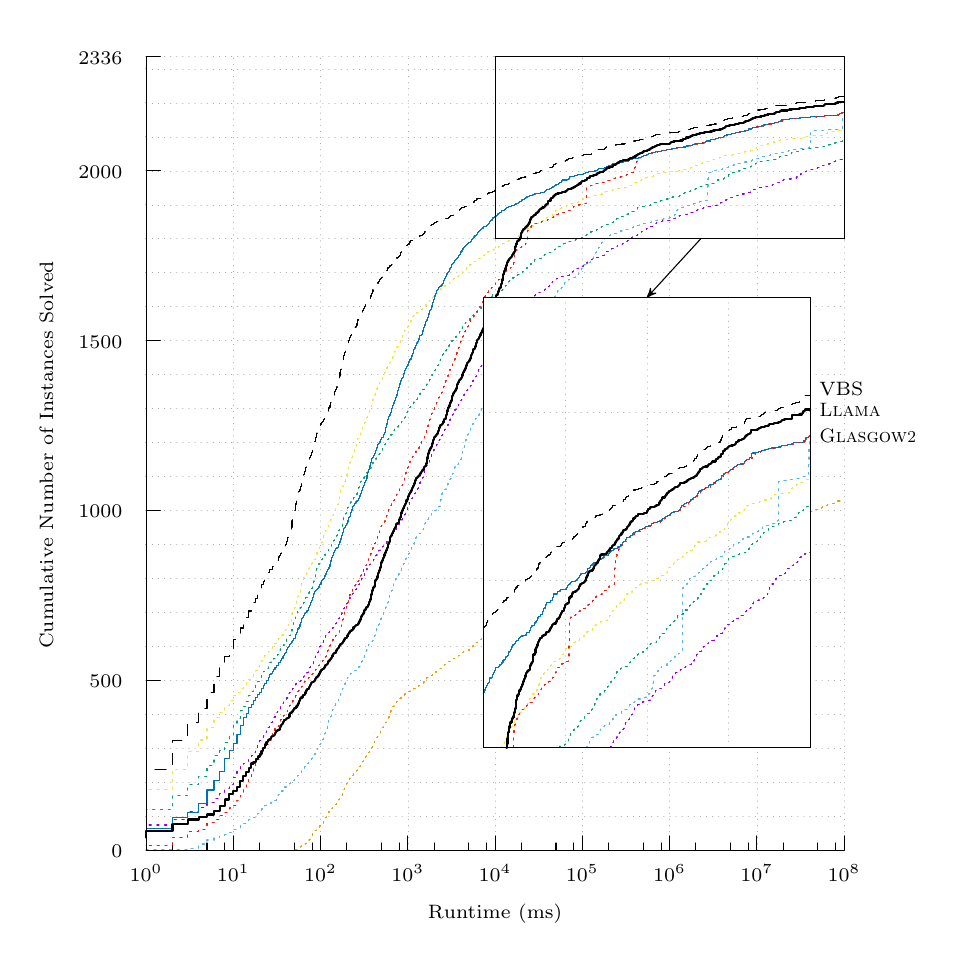
\begin{tikzpicture}[gnuplot]
%% generated with GNUPLOT 5.0p0 (Lua 5.2; terminal rev. 99, script rev. 100)
%% Fri 18 Dec 2015 02:49:10 GMT
\tikzset{every node/.append style={font={\scriptsize}}}
\path (0.000,0.000) rectangle (10.922,11.430);
\gpcolor{color=gp lt color axes}
\gpsetlinetype{gp lt axes}
\gpsetdashtype{gp dt axes}
\gpsetlinewidth{0.50}
\draw[gp path] (1.504,11.061)--(10.368,11.061);
\gpcolor{color=gp lt color border}
\gpsetlinetype{gp lt border}
\gpsetdashtype{gp dt solid}
\gpsetlinewidth{1.00}
\draw[gp path] (1.504,11.061)--(1.684,11.061);
\node[gp node right] at (1.320,11.061) {$2336$};
\gpcolor{color=gp lt color axes}
\gpsetlinetype{gp lt axes}
\gpsetdashtype{gp dt axes}
\gpsetlinewidth{0.50}
\draw[gp path] (1.504,0.985)--(10.368,0.985);
\gpcolor{color=gp lt color border}
\gpsetlinetype{gp lt border}
\gpsetdashtype{gp dt solid}
\gpsetlinewidth{1.00}
\draw[gp path] (1.504,0.985)--(1.684,0.985);
\node[gp node right] at (1.320,0.985) {$0$};
\gpcolor{color=gp lt color axes}
\gpsetlinetype{gp lt axes}
\gpsetdashtype{gp dt axes}
\gpsetlinewidth{0.50}
\draw[gp path] (1.504,1.416)--(10.368,1.416);
\gpcolor{color=gp lt color border}
\gpsetlinetype{gp lt border}
\gpsetdashtype{gp dt solid}
\gpsetlinewidth{1.00}
\draw[gp path] (1.504,1.416)--(1.505,1.416);
\gpcolor{color=gp lt color axes}
\gpsetlinetype{gp lt axes}
\gpsetdashtype{gp dt axes}
\gpsetlinewidth{0.50}
\draw[gp path] (1.504,1.848)--(10.368,1.848);
\gpcolor{color=gp lt color border}
\gpsetlinetype{gp lt border}
\gpsetdashtype{gp dt solid}
\gpsetlinewidth{1.00}
\draw[gp path] (1.504,1.848)--(1.505,1.848);
\gpcolor{color=gp lt color axes}
\gpsetlinetype{gp lt axes}
\gpsetdashtype{gp dt axes}
\gpsetlinewidth{0.50}
\draw[gp path] (1.504,2.279)--(10.368,2.279);
\gpcolor{color=gp lt color border}
\gpsetlinetype{gp lt border}
\gpsetdashtype{gp dt solid}
\gpsetlinewidth{1.00}
\draw[gp path] (1.504,2.279)--(1.505,2.279);
\gpcolor{color=gp lt color axes}
\gpsetlinetype{gp lt axes}
\gpsetdashtype{gp dt axes}
\gpsetlinewidth{0.50}
\draw[gp path] (1.504,2.710)--(10.368,2.710);
\gpcolor{color=gp lt color border}
\gpsetlinetype{gp lt border}
\gpsetdashtype{gp dt solid}
\gpsetlinewidth{1.00}
\draw[gp path] (1.504,2.710)--(1.505,2.710);
\gpcolor{color=gp lt color axes}
\gpsetlinetype{gp lt axes}
\gpsetdashtype{gp dt axes}
\gpsetlinewidth{0.50}
\draw[gp path] (1.504,3.142)--(10.368,3.142);
\gpcolor{color=gp lt color border}
\gpsetlinetype{gp lt border}
\gpsetdashtype{gp dt solid}
\gpsetlinewidth{1.00}
\draw[gp path] (1.504,3.142)--(1.684,3.142);
\node[gp node right] at (1.320,3.142) {$500$};
\gpcolor{color=gp lt color axes}
\gpsetlinetype{gp lt axes}
\gpsetdashtype{gp dt axes}
\gpsetlinewidth{0.50}
\draw[gp path] (1.504,3.573)--(10.368,3.573);
\gpcolor{color=gp lt color border}
\gpsetlinetype{gp lt border}
\gpsetdashtype{gp dt solid}
\gpsetlinewidth{1.00}
\draw[gp path] (1.504,3.573)--(1.505,3.573);
\gpcolor{color=gp lt color axes}
\gpsetlinetype{gp lt axes}
\gpsetdashtype{gp dt axes}
\gpsetlinewidth{0.50}
\draw[gp path] (1.504,4.004)--(10.368,4.004);
\gpcolor{color=gp lt color border}
\gpsetlinetype{gp lt border}
\gpsetdashtype{gp dt solid}
\gpsetlinewidth{1.00}
\draw[gp path] (1.504,4.004)--(1.505,4.004);
\gpcolor{color=gp lt color axes}
\gpsetlinetype{gp lt axes}
\gpsetdashtype{gp dt axes}
\gpsetlinewidth{0.50}
\draw[gp path] (1.504,4.436)--(10.368,4.436);
\gpcolor{color=gp lt color border}
\gpsetlinetype{gp lt border}
\gpsetdashtype{gp dt solid}
\gpsetlinewidth{1.00}
\draw[gp path] (1.504,4.436)--(1.505,4.436);
\gpcolor{color=gp lt color axes}
\gpsetlinetype{gp lt axes}
\gpsetdashtype{gp dt axes}
\gpsetlinewidth{0.50}
\draw[gp path] (1.504,4.867)--(10.368,4.867);
\gpcolor{color=gp lt color border}
\gpsetlinetype{gp lt border}
\gpsetdashtype{gp dt solid}
\gpsetlinewidth{1.00}
\draw[gp path] (1.504,4.867)--(1.505,4.867);
\gpcolor{color=gp lt color axes}
\gpsetlinetype{gp lt axes}
\gpsetdashtype{gp dt axes}
\gpsetlinewidth{0.50}
\draw[gp path] (1.504,5.298)--(10.368,5.298);
\gpcolor{color=gp lt color border}
\gpsetlinetype{gp lt border}
\gpsetdashtype{gp dt solid}
\gpsetlinewidth{1.00}
\draw[gp path] (1.504,5.298)--(1.684,5.298);
\node[gp node right] at (1.320,5.298) {$1000$};
\gpcolor{color=gp lt color axes}
\gpsetlinetype{gp lt axes}
\gpsetdashtype{gp dt axes}
\gpsetlinewidth{0.50}
\draw[gp path] (1.504,5.730)--(10.368,5.730);
\gpcolor{color=gp lt color border}
\gpsetlinetype{gp lt border}
\gpsetdashtype{gp dt solid}
\gpsetlinewidth{1.00}
\draw[gp path] (1.504,5.730)--(1.505,5.730);
\gpcolor{color=gp lt color axes}
\gpsetlinetype{gp lt axes}
\gpsetdashtype{gp dt axes}
\gpsetlinewidth{0.50}
\draw[gp path] (1.504,6.161)--(10.368,6.161);
\gpcolor{color=gp lt color border}
\gpsetlinetype{gp lt border}
\gpsetdashtype{gp dt solid}
\gpsetlinewidth{1.00}
\draw[gp path] (1.504,6.161)--(1.505,6.161);
\gpcolor{color=gp lt color axes}
\gpsetlinetype{gp lt axes}
\gpsetdashtype{gp dt axes}
\gpsetlinewidth{0.50}
\draw[gp path] (1.504,6.592)--(10.368,6.592);
\gpcolor{color=gp lt color border}
\gpsetlinetype{gp lt border}
\gpsetdashtype{gp dt solid}
\gpsetlinewidth{1.00}
\draw[gp path] (1.504,6.592)--(1.505,6.592);
\gpcolor{color=gp lt color axes}
\gpsetlinetype{gp lt axes}
\gpsetdashtype{gp dt axes}
\gpsetlinewidth{0.50}
\draw[gp path] (1.504,7.024)--(10.368,7.024);
\gpcolor{color=gp lt color border}
\gpsetlinetype{gp lt border}
\gpsetdashtype{gp dt solid}
\gpsetlinewidth{1.00}
\draw[gp path] (1.504,7.024)--(1.505,7.024);
\gpcolor{color=gp lt color axes}
\gpsetlinetype{gp lt axes}
\gpsetdashtype{gp dt axes}
\gpsetlinewidth{0.50}
\draw[gp path] (1.504,7.455)--(10.368,7.455);
\gpcolor{color=gp lt color border}
\gpsetlinetype{gp lt border}
\gpsetdashtype{gp dt solid}
\gpsetlinewidth{1.00}
\draw[gp path] (1.504,7.455)--(1.684,7.455);
\node[gp node right] at (1.320,7.455) {$1500$};
\gpcolor{color=gp lt color axes}
\gpsetlinetype{gp lt axes}
\gpsetdashtype{gp dt axes}
\gpsetlinewidth{0.50}
\draw[gp path] (1.504,7.886)--(10.368,7.886);
\gpcolor{color=gp lt color border}
\gpsetlinetype{gp lt border}
\gpsetdashtype{gp dt solid}
\gpsetlinewidth{1.00}
\draw[gp path] (1.504,7.886)--(1.505,7.886);
\gpcolor{color=gp lt color axes}
\gpsetlinetype{gp lt axes}
\gpsetdashtype{gp dt axes}
\gpsetlinewidth{0.50}
\draw[gp path] (1.504,8.318)--(10.368,8.318);
\gpcolor{color=gp lt color border}
\gpsetlinetype{gp lt border}
\gpsetdashtype{gp dt solid}
\gpsetlinewidth{1.00}
\draw[gp path] (1.504,8.318)--(1.505,8.318);
\gpcolor{color=gp lt color axes}
\gpsetlinetype{gp lt axes}
\gpsetdashtype{gp dt axes}
\gpsetlinewidth{0.50}
\draw[gp path] (1.504,8.749)--(10.368,8.749);
\gpcolor{color=gp lt color border}
\gpsetlinetype{gp lt border}
\gpsetdashtype{gp dt solid}
\gpsetlinewidth{1.00}
\draw[gp path] (1.504,8.749)--(1.505,8.749);
\gpcolor{color=gp lt color axes}
\gpsetlinetype{gp lt axes}
\gpsetdashtype{gp dt axes}
\gpsetlinewidth{0.50}
\draw[gp path] (1.504,9.180)--(10.368,9.180);
\gpcolor{color=gp lt color border}
\gpsetlinetype{gp lt border}
\gpsetdashtype{gp dt solid}
\gpsetlinewidth{1.00}
\draw[gp path] (1.504,9.180)--(1.505,9.180);
\gpcolor{color=gp lt color axes}
\gpsetlinetype{gp lt axes}
\gpsetdashtype{gp dt axes}
\gpsetlinewidth{0.50}
\draw[gp path] (1.504,9.612)--(10.368,9.612);
\gpcolor{color=gp lt color border}
\gpsetlinetype{gp lt border}
\gpsetdashtype{gp dt solid}
\gpsetlinewidth{1.00}
\draw[gp path] (1.504,9.612)--(1.684,9.612);
\node[gp node right] at (1.320,9.612) {$2000$};
\gpcolor{color=gp lt color axes}
\gpsetlinetype{gp lt axes}
\gpsetdashtype{gp dt axes}
\gpsetlinewidth{0.50}
\draw[gp path] (1.504,10.043)--(10.368,10.043);
\gpcolor{color=gp lt color border}
\gpsetlinetype{gp lt border}
\gpsetdashtype{gp dt solid}
\gpsetlinewidth{1.00}
\draw[gp path] (1.504,10.043)--(1.505,10.043);
\gpcolor{color=gp lt color axes}
\gpsetlinetype{gp lt axes}
\gpsetdashtype{gp dt axes}
\gpsetlinewidth{0.50}
\draw[gp path] (1.504,10.474)--(10.368,10.474);
\gpcolor{color=gp lt color border}
\gpsetlinetype{gp lt border}
\gpsetdashtype{gp dt solid}
\gpsetlinewidth{1.00}
\draw[gp path] (1.504,10.474)--(1.505,10.474);
\gpcolor{color=gp lt color axes}
\gpsetlinetype{gp lt axes}
\gpsetdashtype{gp dt axes}
\gpsetlinewidth{0.50}
\draw[gp path] (1.504,10.906)--(10.368,10.906);
\gpcolor{color=gp lt color border}
\gpsetlinetype{gp lt border}
\gpsetdashtype{gp dt solid}
\gpsetlinewidth{1.00}
\draw[gp path] (1.504,10.906)--(1.505,10.906);
\gpcolor{color=gp lt color axes}
\gpsetlinetype{gp lt axes}
\gpsetdashtype{gp dt axes}
\gpsetlinewidth{0.50}
\draw[gp path] (1.504,0.985)--(1.504,11.061);
\gpcolor{color=gp lt color border}
\gpsetlinetype{gp lt border}
\gpsetdashtype{gp dt solid}
\gpsetlinewidth{1.00}
\draw[gp path] (1.504,0.985)--(1.504,1.165);
\node[gp node center] at (1.504,0.677) {$10^{0}$};
\draw[gp path] (1.838,0.985)--(1.838,1.075);
\draw[gp path] (2.278,0.985)--(2.278,1.075);
\draw[gp path] (2.505,0.985)--(2.505,1.075);
\gpcolor{color=gp lt color axes}
\gpsetlinetype{gp lt axes}
\gpsetdashtype{gp dt axes}
\gpsetlinewidth{0.50}
\draw[gp path] (2.612,0.985)--(2.612,11.061);
\gpcolor{color=gp lt color border}
\gpsetlinetype{gp lt border}
\gpsetdashtype{gp dt solid}
\gpsetlinewidth{1.00}
\draw[gp path] (2.612,0.985)--(2.612,1.165);
\node[gp node center] at (2.612,0.677) {$10^{1}$};
\draw[gp path] (2.946,0.985)--(2.946,1.075);
\draw[gp path] (3.386,0.985)--(3.386,1.075);
\draw[gp path] (3.613,0.985)--(3.613,1.075);
\gpcolor{color=gp lt color axes}
\gpsetlinetype{gp lt axes}
\gpsetdashtype{gp dt axes}
\gpsetlinewidth{0.50}
\draw[gp path] (3.720,0.985)--(3.720,11.061);
\gpcolor{color=gp lt color border}
\gpsetlinetype{gp lt border}
\gpsetdashtype{gp dt solid}
\gpsetlinewidth{1.00}
\draw[gp path] (3.720,0.985)--(3.720,1.165);
\node[gp node center] at (3.720,0.677) {$10^{2}$};
\draw[gp path] (4.054,0.985)--(4.054,1.075);
\draw[gp path] (4.494,0.985)--(4.494,1.075);
\draw[gp path] (4.721,0.985)--(4.721,1.075);
\gpcolor{color=gp lt color axes}
\gpsetlinetype{gp lt axes}
\gpsetdashtype{gp dt axes}
\gpsetlinewidth{0.50}
\draw[gp path] (4.828,0.985)--(4.828,11.061);
\gpcolor{color=gp lt color border}
\gpsetlinetype{gp lt border}
\gpsetdashtype{gp dt solid}
\gpsetlinewidth{1.00}
\draw[gp path] (4.828,0.985)--(4.828,1.165);
\node[gp node center] at (4.828,0.677) {$10^{3}$};
\draw[gp path] (5.162,0.985)--(5.162,1.075);
\draw[gp path] (5.602,0.985)--(5.602,1.075);
\draw[gp path] (5.829,0.985)--(5.829,1.075);
\gpcolor{color=gp lt color axes}
\gpsetlinetype{gp lt axes}
\gpsetdashtype{gp dt axes}
\gpsetlinewidth{0.50}
\draw[gp path] (5.936,0.985)--(5.936,11.061);
\gpcolor{color=gp lt color border}
\gpsetlinetype{gp lt border}
\gpsetdashtype{gp dt solid}
\gpsetlinewidth{1.00}
\draw[gp path] (5.936,0.985)--(5.936,1.165);
\node[gp node center] at (5.936,0.677) {$10^{4}$};
\draw[gp path] (6.270,0.985)--(6.270,1.075);
\draw[gp path] (6.710,0.985)--(6.710,1.075);
\draw[gp path] (6.937,0.985)--(6.937,1.075);
\gpcolor{color=gp lt color axes}
\gpsetlinetype{gp lt axes}
\gpsetdashtype{gp dt axes}
\gpsetlinewidth{0.50}
\draw[gp path] (7.044,0.985)--(7.044,11.061);
\gpcolor{color=gp lt color border}
\gpsetlinetype{gp lt border}
\gpsetdashtype{gp dt solid}
\gpsetlinewidth{1.00}
\draw[gp path] (7.044,0.985)--(7.044,1.165);
\node[gp node center] at (7.044,0.677) {$10^{5}$};
\draw[gp path] (7.378,0.985)--(7.378,1.075);
\draw[gp path] (7.818,0.985)--(7.818,1.075);
\draw[gp path] (8.045,0.985)--(8.045,1.075);
\gpcolor{color=gp lt color axes}
\gpsetlinetype{gp lt axes}
\gpsetdashtype{gp dt axes}
\gpsetlinewidth{0.50}
\draw[gp path] (8.152,0.985)--(8.152,11.061);
\gpcolor{color=gp lt color border}
\gpsetlinetype{gp lt border}
\gpsetdashtype{gp dt solid}
\gpsetlinewidth{1.00}
\draw[gp path] (8.152,0.985)--(8.152,1.165);
\node[gp node center] at (8.152,0.677) {$10^{6}$};
\draw[gp path] (8.486,0.985)--(8.486,1.075);
\draw[gp path] (8.926,0.985)--(8.926,1.075);
\draw[gp path] (9.153,0.985)--(9.153,1.075);
\gpcolor{color=gp lt color axes}
\gpsetlinetype{gp lt axes}
\gpsetdashtype{gp dt axes}
\gpsetlinewidth{0.50}
\draw[gp path] (9.260,0.985)--(9.260,11.061);
\gpcolor{color=gp lt color border}
\gpsetlinetype{gp lt border}
\gpsetdashtype{gp dt solid}
\gpsetlinewidth{1.00}
\draw[gp path] (9.260,0.985)--(9.260,1.165);
\node[gp node center] at (9.260,0.677) {$10^{7}$};
\draw[gp path] (9.594,0.985)--(9.594,1.075);
\draw[gp path] (10.034,0.985)--(10.034,1.075);
\draw[gp path] (10.261,0.985)--(10.261,1.075);
\gpcolor{color=gp lt color axes}
\gpsetlinetype{gp lt axes}
\gpsetdashtype{gp dt axes}
\gpsetlinewidth{0.50}
\draw[gp path] (10.368,0.985)--(10.368,11.061);
\gpcolor{color=gp lt color border}
\gpsetlinetype{gp lt border}
\gpsetdashtype{gp dt solid}
\gpsetlinewidth{1.00}
\draw[gp path] (10.368,0.985)--(10.368,1.165);
\node[gp node center] at (10.368,0.677) {$10^{8}$};
\draw[gp path] (1.504,11.061)--(1.504,0.985)--(10.368,0.985);
\node[gp node center,rotate=-270] at (0.246,6.023) {Cumulative Number of Instances Solved};
\node[gp node center] at (5.936,0.215) {Runtime (ms)};
\gpcolor{rgb color={0.580,0.000,0.827}}
\gpsetdashtype{dash pattern=on 2.00*\gpdashlength off 5.00*\gpdashlength }
\draw[gp path] (1.504,1.145)--(1.504,1.304)--(1.838,1.304)--(1.838,1.378)--(2.033,1.378)%
  --(2.033,1.472)--(2.171,1.472)--(2.171,1.524)--(2.278,1.524)--(2.278,1.585)--(2.366,1.585)%
  --(2.366,1.636)--(2.440,1.636)--(2.440,1.705)--(2.505,1.705)--(2.505,1.766)--(2.561,1.766)%
  --(2.561,1.817)--(2.612,1.817)--(2.612,1.908)--(2.658,1.908)--(2.658,1.990)--(2.700,1.990)%
  --(2.700,2.059)--(2.738,2.059)--(2.738,2.089)--(2.774,2.089)--(2.774,2.106)--(2.807,2.106)%
  --(2.807,2.141)--(2.838,2.141)--(2.838,2.184)--(2.867,2.184)--(2.867,2.219)--(2.895,2.219)%
  --(2.895,2.283)--(2.921,2.283)--(2.921,2.331)--(2.946,2.331)--(2.946,2.374)--(2.969,2.374)%
  --(2.969,2.408)--(2.991,2.408)--(2.991,2.434)--(3.013,2.434)--(3.013,2.473)--(3.033,2.473)%
  --(3.033,2.508)--(3.053,2.508)--(3.053,2.546)--(3.072,2.546)--(3.072,2.585)--(3.090,2.585)%
  --(3.090,2.607)--(3.107,2.607)--(3.107,2.646)--(3.124,2.646)--(3.124,2.672)--(3.141,2.672)%
  --(3.141,2.706)--(3.156,2.706)--(3.156,2.732)--(3.172,2.732)--(3.172,2.749)--(3.187,2.749)%
  --(3.187,2.753)--(3.201,2.753)--(3.201,2.775)--(3.215,2.775)--(3.215,2.810)--(3.228,2.810)%
  --(3.228,2.835)--(3.242,2.835)--(3.242,2.848)--(3.254,2.848)--(3.254,2.870)--(3.267,2.870)%
  --(3.267,2.883)--(3.279,2.883)--(3.279,2.900)--(3.291,2.900)--(3.291,2.917)--(3.303,2.917)%
  --(3.303,2.952)--(3.314,2.952)--(3.314,2.973)--(3.325,2.973)--(3.325,2.982)--(3.346,2.982)%
  --(3.346,2.986)--(3.357,2.986)--(3.357,3.012)--(3.367,3.012)--(3.367,3.038)--(3.377,3.038)%
  --(3.377,3.042)--(3.386,3.042)--(3.386,3.068)--(3.396,3.068)--(3.396,3.081)--(3.405,3.081)%
  --(3.405,3.094)--(3.414,3.094)--(3.414,3.107)--(3.432,3.107)--(3.432,3.120)--(3.450,3.120)%
  --(3.450,3.124)--(3.458,3.124)--(3.458,3.129)--(3.466,3.129)--(3.466,3.137)--(3.474,3.137)%
  --(3.474,3.159)--(3.482,3.159)--(3.482,3.163)--(3.490,3.163)--(3.490,3.168)--(3.505,3.168)%
  --(3.505,3.185)--(3.513,3.185)--(3.513,3.211)--(3.527,3.211)--(3.527,3.215)--(3.534,3.215)%
  --(3.534,3.219)--(3.541,3.219)--(3.541,3.232)--(3.548,3.232)--(3.548,3.245)--(3.562,3.245)%
  --(3.562,3.254)--(3.569,3.254)--(3.569,3.262)--(3.575,3.262)--(3.575,3.271)--(3.582,3.271)%
  --(3.582,3.301)--(3.588,3.301)--(3.588,3.314)--(3.594,3.314)--(3.594,3.319)--(3.600,3.319)%
  --(3.600,3.331)--(3.607,3.331)--(3.607,3.340)--(3.613,3.340)--(3.613,3.349)--(3.625,3.349)%
  --(3.625,3.362)--(3.630,3.362)--(3.630,3.383)--(3.636,3.383)--(3.636,3.396)--(3.642,3.396)%
  --(3.642,3.409)--(3.647,3.409)--(3.647,3.426)--(3.653,3.426)--(3.653,3.439)--(3.658,3.439)%
  --(3.658,3.448)--(3.664,3.448)--(3.664,3.457)--(3.669,3.457)--(3.669,3.465)--(3.675,3.465)%
  --(3.675,3.474)--(3.680,3.474)--(3.680,3.482)--(3.685,3.482)--(3.685,3.491)--(3.690,3.491)%
  --(3.690,3.530)--(3.695,3.530)--(3.695,3.534)--(3.700,3.534)--(3.700,3.547)--(3.705,3.547)%
  --(3.705,3.551)--(3.710,3.551)--(3.710,3.569)--(3.715,3.569)--(3.715,3.573)--(3.720,3.573)%
  --(3.720,3.577)--(3.730,3.577)--(3.730,3.582)--(3.734,3.582)--(3.734,3.590)--(3.739,3.590)%
  --(3.739,3.608)--(3.743,3.608)--(3.743,3.612)--(3.748,3.612)--(3.748,3.620)--(3.753,3.620)%
  --(3.753,3.629)--(3.757,3.629)--(3.757,3.642)--(3.766,3.642)--(3.766,3.646)--(3.770,3.646)%
  --(3.770,3.659)--(3.775,3.659)--(3.775,3.681)--(3.779,3.681)--(3.779,3.685)--(3.783,3.685)%
  --(3.783,3.707)--(3.787,3.707)--(3.787,3.711)--(3.791,3.711)--(3.791,3.720)--(3.796,3.720)%
  --(3.796,3.724)--(3.804,3.724)--(3.804,3.728)--(3.808,3.728)--(3.808,3.733)--(3.812,3.733)%
  --(3.812,3.741)--(3.816,3.741)--(3.816,3.746)--(3.820,3.746)--(3.820,3.750)--(3.824,3.750)%
  --(3.824,3.754)--(3.831,3.754)--(3.831,3.763)--(3.835,3.763)--(3.835,3.767)--(3.843,3.767)%
  --(3.843,3.771)--(3.846,3.771)--(3.846,3.780)--(3.854,3.780)--(3.854,3.784)--(3.861,3.784)%
  --(3.861,3.789)--(3.864,3.789)--(3.864,3.793)--(3.868,3.793)--(3.868,3.797)--(3.871,3.797)%
  --(3.871,3.802)--(3.875,3.802)--(3.875,3.806)--(3.878,3.806)--(3.878,3.810)--(3.882,3.810)%
  --(3.882,3.815)--(3.885,3.815)--(3.885,3.828)--(3.895,3.828)--(3.895,3.840)--(3.899,3.840)%
  --(3.899,3.849)--(3.905,3.849)--(3.905,3.853)--(3.909,3.853)--(3.909,3.858)--(3.915,3.858)%
  --(3.915,3.866)--(3.918,3.866)--(3.918,3.875)--(3.921,3.875)--(3.921,3.888)--(3.925,3.888)%
  --(3.925,3.892)--(3.928,3.892)--(3.928,3.901)--(3.934,3.901)--(3.934,3.909)--(3.940,3.909)%
  --(3.940,3.914)--(3.943,3.914)--(3.943,3.922)--(3.949,3.922)--(3.949,3.927)--(3.952,3.927)%
  --(3.952,3.931)--(3.955,3.931)--(3.955,3.935)--(3.958,3.935)--(3.958,3.940)--(3.964,3.940)%
  --(3.964,3.944)--(3.967,3.944)--(3.967,3.948)--(3.970,3.948)--(3.970,3.953)--(3.972,3.953)%
  --(3.972,3.957)--(3.975,3.957)--(3.975,3.961)--(3.981,3.961)--(3.981,3.966)--(3.984,3.966)%
  --(3.984,3.970)--(3.987,3.970)--(3.987,3.978)--(3.989,3.978)--(3.989,3.991)--(3.992,3.991)%
  --(3.992,4.000)--(4.000,4.000)--(4.000,4.009)--(4.003,4.009)--(4.003,4.030)--(4.006,4.030)%
  --(4.006,4.039)--(4.008,4.039)--(4.008,4.043)--(4.011,4.043)--(4.011,4.047)--(4.013,4.047)%
  --(4.013,4.052)--(4.019,4.052)--(4.019,4.056)--(4.021,4.056)--(4.021,4.069)--(4.024,4.069)%
  --(4.024,4.073)--(4.026,4.073)--(4.026,4.078)--(4.031,4.078)--(4.031,4.082)--(4.036,4.082)%
  --(4.036,4.086)--(4.041,4.086)--(4.041,4.099)--(4.044,4.099)--(4.044,4.104)--(4.049,4.104)%
  --(4.049,4.108)--(4.051,4.108)--(4.051,4.112)--(4.054,4.112)--(4.054,4.116)--(4.056,4.116)%
  --(4.056,4.121)--(4.058,4.121)--(4.058,4.125)--(4.061,4.125)--(4.061,4.129)--(4.063,4.129)%
  --(4.063,4.134)--(4.068,4.134)--(4.068,4.142)--(4.070,4.142)--(4.070,4.151)--(4.077,4.151)%
  --(4.077,4.164)--(4.082,4.164)--(4.082,4.177)--(4.086,4.177)--(4.086,4.181)--(4.091,4.181)%
  --(4.091,4.186)--(4.093,4.186)--(4.093,4.194)--(4.097,4.194)--(4.097,4.198)--(4.102,4.198)%
  --(4.102,4.211)--(4.110,4.211)--(4.110,4.220)--(4.112,4.220)--(4.112,4.224)--(4.119,4.224)%
  --(4.119,4.229)--(4.121,4.229)--(4.121,4.233)--(4.123,4.233)--(4.123,4.237)--(4.129,4.237)%
  --(4.129,4.242)--(4.133,4.242)--(4.133,4.246)--(4.135,4.246)--(4.135,4.250)--(4.139,4.250)%
  --(4.139,4.259)--(4.141,4.259)--(4.141,4.267)--(4.149,4.267)--(4.149,4.276)--(4.155,4.276)%
  --(4.155,4.285)--(4.157,4.285)--(4.157,4.289)--(4.163,4.289)--(4.163,4.293)--(4.172,4.293)%
  --(4.172,4.298)--(4.174,4.298)--(4.174,4.306)--(4.180,4.306)--(4.180,4.315)--(4.183,4.315)%
  --(4.183,4.319)--(4.191,4.319)--(4.191,4.324)--(4.193,4.324)--(4.193,4.332)--(4.194,4.332)%
  --(4.194,4.341)--(4.196,4.341)--(4.196,4.349)--(4.198,4.349)--(4.198,4.354)--(4.200,4.354)%
  --(4.200,4.358)--(4.207,4.358)--(4.207,4.362)--(4.210,4.362)--(4.210,4.371)--(4.212,4.371)%
  --(4.212,4.380)--(4.215,4.380)--(4.215,4.384)--(4.219,4.384)--(4.219,4.388)--(4.221,4.388)%
  --(4.221,4.393)--(4.222,4.393)--(4.222,4.397)--(4.224,4.397)--(4.224,4.401)--(4.227,4.401)%
  --(4.227,4.405)--(4.234,4.405)--(4.234,4.410)--(4.236,4.410)--(4.236,4.418)--(4.241,4.418)%
  --(4.241,4.427)--(4.242,4.427)--(4.242,4.431)--(4.255,4.431)--(4.255,4.440)--(4.258,4.440)%
  --(4.258,4.444)--(4.260,4.444)--(4.260,4.449)--(4.261,4.449)--(4.261,4.462)--(4.263,4.462)%
  --(4.263,4.466)--(4.271,4.466)--(4.271,4.470)--(4.275,4.470)--(4.275,4.475)--(4.277,4.475)%
  --(4.277,4.479)--(4.278,4.479)--(4.278,4.483)--(4.280,4.483)--(4.280,4.487)--(4.283,4.487)%
  --(4.283,4.496)--(4.289,4.496)--(4.289,4.500)--(4.292,4.500)--(4.292,4.509)--(4.293,4.509)%
  --(4.293,4.513)--(4.296,4.513)--(4.296,4.526)--(4.299,4.526)--(4.299,4.531)--(4.303,4.531)%
  --(4.303,4.535)--(4.305,4.535)--(4.305,4.544)--(4.306,4.544)--(4.306,4.548)--(4.307,4.548)%
  --(4.307,4.552)--(4.309,4.552)--(4.309,4.556)--(4.310,4.556)--(4.310,4.565)--(4.319,4.565)%
  --(4.319,4.569)--(4.320,4.569)--(4.320,4.574)--(4.321,4.574)--(4.321,4.578)--(4.323,4.578)%
  --(4.323,4.582)--(4.326,4.582)--(4.326,4.587)--(4.327,4.587)--(4.327,4.591)--(4.328,4.591)%
  --(4.328,4.595)--(4.338,4.595)--(4.338,4.604)--(4.343,4.604)--(4.343,4.608)--(4.346,4.608)%
  --(4.346,4.617)--(4.355,4.617)--(4.355,4.621)--(4.359,4.621)--(4.359,4.630)--(4.369,4.630)%
  --(4.369,4.634)--(4.370,4.634)--(4.370,4.638)--(4.371,4.638)--(4.371,4.643)--(4.375,4.643)%
  --(4.375,4.647)--(4.379,4.647)--(4.379,4.651)--(4.381,4.651)--(4.381,4.656)--(4.388,4.656)%
  --(4.388,4.660)--(4.389,4.660)--(4.389,4.664)--(4.394,4.664)--(4.394,4.669)--(4.397,4.669)%
  --(4.397,4.673)--(4.402,4.673)--(4.402,4.677)--(4.405,4.677)--(4.405,4.682)--(4.406,4.682)%
  --(4.406,4.686)--(4.407,4.686)--(4.407,4.690)--(4.409,4.690)--(4.409,4.694)--(4.412,4.694)%
  --(4.412,4.699)--(4.414,4.699)--(4.414,4.703)--(4.415,4.703)--(4.415,4.712)--(4.417,4.712)%
  --(4.417,4.716)--(4.420,4.716)--(4.420,4.720)--(4.421,4.720)--(4.421,4.725)--(4.423,4.725)%
  --(4.423,4.729)--(4.430,4.729)--(4.430,4.733)--(4.437,4.733)--(4.437,4.738)--(4.441,4.738)%
  --(4.441,4.742)--(4.443,4.742)--(4.443,4.746)--(4.445,4.746)--(4.445,4.751)--(4.447,4.751)%
  --(4.447,4.755)--(4.448,4.755)--(4.448,4.764)--(4.452,4.764)--(4.452,4.768)--(4.453,4.768)%
  --(4.453,4.772)--(4.454,4.772)--(4.454,4.776)--(4.459,4.776)--(4.459,4.781)--(4.460,4.781)%
  --(4.460,4.785)--(4.470,4.785)--(4.470,4.794)--(4.475,4.794)--(4.475,4.798)--(4.482,4.798)%
  --(4.482,4.802)--(4.483,4.802)--(4.483,4.807)--(4.491,4.807)--(4.491,4.811)--(4.496,4.811)%
  --(4.496,4.820)--(4.498,4.820)--(4.498,4.824)--(4.499,4.824)--(4.499,4.828)--(4.501,4.828)%
  --(4.501,4.833)--(4.507,4.833)--(4.507,4.837)--(4.508,4.837)--(4.508,4.841)--(4.518,4.841)%
  --(4.518,4.845)--(4.519,4.845)--(4.519,4.850)--(4.523,4.850)--(4.523,4.854)--(4.529,4.854)%
  --(4.529,4.858)--(4.530,4.858)--(4.530,4.863)--(4.542,4.863)--(4.542,4.867)--(4.544,4.867)%
  --(4.544,4.876)--(4.547,4.876)--(4.547,4.880)--(4.551,4.880)--(4.551,4.884)--(4.557,4.884)%
  --(4.557,4.889)--(4.558,4.889)--(4.558,4.893)--(4.561,4.893)--(4.561,4.897)--(4.563,4.897)%
  --(4.563,4.902)--(4.564,4.902)--(4.564,4.906)--(4.567,4.906)--(4.567,4.910)--(4.577,4.910)%
  --(4.577,4.914)--(4.580,4.914)--(4.580,4.923)--(4.582,4.923)--(4.582,4.927)--(4.586,4.927)%
  --(4.586,4.932)--(4.587,4.932)--(4.587,4.936)--(4.590,4.936)--(4.590,4.940)--(4.593,4.940)%
  --(4.593,4.949)--(4.599,4.949)--(4.599,4.953)--(4.600,4.953)--(4.600,4.958)--(4.603,4.958)%
  --(4.603,4.962)--(4.604,4.962)--(4.604,4.971)--(4.609,4.971)--(4.609,4.975)--(4.620,4.975)%
  --(4.620,4.979)--(4.621,4.979)--(4.621,4.983)--(4.623,4.983)--(4.623,4.988)--(4.628,4.988)%
  --(4.628,4.992)--(4.635,4.992)--(4.635,4.996)--(4.636,4.996)--(4.636,5.001)--(4.637,5.001)%
  --(4.637,5.005)--(4.641,5.005)--(4.641,5.009)--(4.644,5.009)--(4.644,5.014)--(4.649,5.014)%
  --(4.649,5.018)--(4.653,5.018)--(4.653,5.022)--(4.656,5.022)--(4.656,5.027)--(4.657,5.027)%
  --(4.657,5.035)--(4.658,5.035)--(4.658,5.040)--(4.661,5.040)--(4.661,5.044)--(4.669,5.044)%
  --(4.669,5.048)--(4.669,5.052)--(4.671,5.052)--(4.671,5.057)--(4.679,5.057)--(4.679,5.061)%
  --(4.679,5.065)--(4.684,5.065)--(4.684,5.070)--(4.686,5.070)--(4.686,5.074)--(4.686,5.078)%
  --(4.688,5.078)--(4.688,5.083)--(4.691,5.083)--(4.691,5.087)--(4.693,5.087)--(4.693,5.091)%
  --(4.693,5.096)--(4.706,5.096)--(4.706,5.100)--(4.707,5.100)--(4.707,5.104)--(4.709,5.104)%
  --(4.709,5.109)--(4.710,5.109)--(4.710,5.113)--(4.711,5.113)--(4.711,5.122)--(4.719,5.122)%
  --(4.719,5.126)--(4.722,5.126)--(4.722,5.130)--(4.723,5.130)--(4.723,5.134)--(4.726,5.134)%
  --(4.726,5.139)--(4.728,5.139)--(4.728,5.147)--(4.729,5.147)--(4.729,5.152)--(4.732,5.152)%
  --(4.732,5.156)--(4.734,5.156)--(4.734,5.160)--(4.743,5.160)--(4.743,5.165)--(4.745,5.165)%
  --(4.745,5.169)--(4.753,5.169)--(4.753,5.173)--(4.754,5.173)--(4.754,5.182)--(4.754,5.186)%
  --(4.757,5.186)--(4.757,5.191)--(4.763,5.191)--(4.763,5.199)--(4.764,5.199)--(4.764,5.203)%
  --(4.766,5.203)--(4.766,5.208)--(4.767,5.208)--(4.767,5.212)--(4.768,5.212)--(4.768,5.216)%
  --(4.769,5.216)--(4.769,5.221)--(4.770,5.221)--(4.770,5.225)--(4.772,5.225)--(4.772,5.234)%
  --(4.783,5.234)--(4.783,5.238)--(4.789,5.238)--(4.789,5.242)--(4.789,5.247)--(4.792,5.247)%
  --(4.792,5.251)--(4.794,5.251)--(4.794,5.255)--(4.794,5.260)--(4.795,5.260)--(4.795,5.264)%
  --(4.796,5.264)--(4.796,5.268)--(4.798,5.268)--(4.798,5.272)--(4.800,5.272)--(4.800,5.277)%
  --(4.804,5.277)--(4.804,5.281)--(4.807,5.281)--(4.807,5.290)--(4.809,5.290)--(4.809,5.294)%
  --(4.810,5.294)--(4.810,5.298)--(4.812,5.298)--(4.812,5.303)--(4.816,5.303)--(4.816,5.307)%
  --(4.819,5.307)--(4.819,5.316)--(4.821,5.316)--(4.821,5.320)--(4.821,5.324)--(4.822,5.324)%
  --(4.822,5.329)--(4.823,5.329)--(4.823,5.333)--(4.823,5.337)--(4.827,5.337)--(4.827,5.341)%
  --(4.832,5.341)--(4.832,5.346)--(4.833,5.346)--(4.833,5.350)--(4.837,5.350)--(4.837,5.354)%
  --(4.838,5.354)--(4.838,5.363)--(4.840,5.363)--(4.840,5.367)--(4.843,5.367)--(4.843,5.372)%
  --(4.848,5.372)--(4.848,5.376)--(4.849,5.376)--(4.849,5.380)--(4.850,5.380)--(4.850,5.385)%
  --(4.851,5.385)--(4.851,5.389)--(4.851,5.393)--(4.852,5.393)--(4.852,5.398)--(4.853,5.398)%
  --(4.853,5.411)--(4.855,5.411)--(4.855,5.419)--(4.856,5.419)--(4.856,5.423)--(4.861,5.423)%
  --(4.861,5.428)--(4.865,5.428)--(4.865,5.432)--(4.869,5.432)--(4.869,5.436)--(4.869,5.441)%
  --(4.873,5.441)--(4.873,5.445)--(4.876,5.445)--(4.876,5.449)--(4.882,5.449)--(4.882,5.454)%
  --(4.886,5.454)--(4.886,5.458)--(4.886,5.462)--(4.889,5.462)--(4.889,5.467)--(4.893,5.467)%
  --(4.893,5.471)--(4.893,5.475)--(4.897,5.475)--(4.897,5.480)--(4.897,5.484)--(4.902,5.484)%
  --(4.902,5.492)--(4.904,5.492)--(4.904,5.497)--(4.906,5.497)--(4.906,5.505)--(4.907,5.505)%
  --(4.907,5.510)--(4.913,5.510)--(4.913,5.514)--(4.917,5.514)--(4.917,5.518)--(4.921,5.518)%
  --(4.921,5.523)--(4.921,5.527)--(4.926,5.527)--(4.926,5.531)--(4.927,5.531)--(4.927,5.536)%
  --(4.932,5.536)--(4.932,5.540)--(4.938,5.540)--(4.938,5.544)--(4.940,5.544)--(4.940,5.549)%
  --(4.941,5.549)--(4.941,5.553)--(4.943,5.553)--(4.943,5.557)--(4.944,5.557)--(4.944,5.561)%
  --(4.950,5.561)--(4.950,5.566)--(4.950,5.570)--(4.954,5.570)--(4.954,5.579)--(4.958,5.579)%
  --(4.958,5.583)--(4.958,5.587)--(4.960,5.587)--(4.960,5.592)--(4.963,5.592)--(4.963,5.596)%
  --(4.964,5.596)--(4.964,5.600)--(4.966,5.600)--(4.966,5.605)--(4.971,5.605)--(4.971,5.609)%
  --(4.972,5.609)--(4.972,5.613)--(4.973,5.613)--(4.973,5.618)--(4.974,5.618)--(4.974,5.622)%
  --(4.976,5.622)--(4.976,5.630)--(4.976,5.635)--(4.977,5.635)--(4.977,5.639)--(4.980,5.639)%
  --(4.980,5.643)--(4.982,5.643)--(4.982,5.648)--(4.983,5.648)--(4.983,5.652)--(4.984,5.652)%
  --(4.984,5.656)--(4.986,5.656)--(4.986,5.661)--(4.987,5.661)--(4.987,5.665)--(4.989,5.665)%
  --(4.989,5.669)--(4.991,5.669)--(4.991,5.674)--(4.994,5.674)--(4.994,5.678)--(4.998,5.678)%
  --(4.998,5.682)--(5.000,5.682)--(5.000,5.687)--(5.004,5.687)--(5.004,5.691)--(5.005,5.691)%
  --(5.005,5.695)--(5.005,5.699)--(5.011,5.699)--(5.011,5.708)--(5.016,5.708)--(5.016,5.712)%
  --(5.019,5.712)--(5.019,5.717)--(5.020,5.717)--(5.020,5.721)--(5.023,5.721)--(5.023,5.725)%
  --(5.025,5.725)--(5.025,5.734)--(5.026,5.734)--(5.026,5.738)--(5.026,5.743)--(5.030,5.743)%
  --(5.030,5.756)--(5.031,5.756)--(5.031,5.760)--(5.032,5.760)--(5.032,5.764)--(5.034,5.764)%
  --(5.034,5.773)--(5.036,5.773)--(5.036,5.781)--(5.037,5.781)--(5.037,5.786)--(5.039,5.786)%
  --(5.039,5.790)--(5.039,5.794)--(5.040,5.794)--(5.040,5.799)--(5.040,5.803)--(5.041,5.803)%
  --(5.041,5.807)--(5.043,5.807)--(5.043,5.820)--(5.045,5.820)--(5.045,5.825)--(5.048,5.825)%
  --(5.048,5.829)--(5.049,5.829)--(5.049,5.833)--(5.051,5.833)--(5.051,5.838)--(5.053,5.838)%
  --(5.053,5.842)--(5.054,5.842)--(5.054,5.846)--(5.057,5.846)--(5.057,5.850)--(5.059,5.850)%
  --(5.059,5.855)--(5.059,5.859)--(5.060,5.859)--(5.060,5.863)--(5.061,5.863)--(5.061,5.868)%
  --(5.064,5.868)--(5.064,5.872)--(5.071,5.872)--(5.071,5.876)--(5.078,5.876)--(5.078,5.881)%
  --(5.082,5.881)--(5.082,5.885)--(5.083,5.885)--(5.083,5.889)--(5.084,5.889)--(5.084,5.894)%
  --(5.090,5.894)--(5.090,5.898)--(5.093,5.898)--(5.093,5.907)--(5.098,5.907)--(5.098,5.911)%
  --(5.100,5.911)--(5.100,5.915)--(5.102,5.915)--(5.102,5.919)--(5.103,5.919)--(5.103,5.924)%
  --(5.103,5.928)--(5.104,5.928)--(5.104,5.932)--(5.106,5.932)--(5.106,5.937)--(5.111,5.937)%
  --(5.111,5.941)--(5.116,5.941)--(5.116,5.945)--(5.117,5.945)--(5.117,5.950)--(5.117,5.954)%
  --(5.121,5.954)--(5.121,5.958)--(5.121,5.971)--(5.122,5.971)--(5.122,5.976)--(5.122,5.980)%
  --(5.125,5.980)--(5.125,5.984)--(5.130,5.984)--(5.130,5.993)--(5.131,5.993)--(5.131,5.997)%
  --(5.131,6.001)--(5.132,6.001)--(5.132,6.006)--(5.134,6.006)--(5.134,6.010)--(5.134,6.014)%
  --(5.136,6.014)--(5.136,6.019)--(5.146,6.019)--(5.146,6.023)--(5.147,6.023)--(5.147,6.032)%
  --(5.148,6.032)--(5.148,6.036)--(5.149,6.036)--(5.149,6.040)--(5.149,6.045)--(5.154,6.045)%
  --(5.154,6.049)--(5.155,6.049)--(5.155,6.053)--(5.156,6.053)--(5.156,6.058)--(5.156,6.066)%
  --(5.163,6.066)--(5.163,6.075)--(5.165,6.075)--(5.165,6.079)--(5.166,6.079)--(5.166,6.083)%
  --(5.168,6.083)--(5.168,6.088)--(5.171,6.088)--(5.171,6.096)--(5.174,6.096)--(5.174,6.101)%
  --(5.177,6.101)--(5.177,6.105)--(5.181,6.105)--(5.181,6.109)--(5.186,6.109)--(5.186,6.114)%
  --(5.187,6.114)--(5.187,6.118)--(5.189,6.118)--(5.189,6.122)--(5.189,6.127)--(5.192,6.127)%
  --(5.192,6.131)--(5.194,6.131)--(5.194,6.135)--(5.201,6.135)--(5.201,6.139)--(5.203,6.139)%
  --(5.203,6.144)--(5.206,6.144)--(5.206,6.148)--(5.206,6.152)--(5.208,6.152)--(5.208,6.157)%
  --(5.210,6.157)--(5.210,6.161)--(5.211,6.161)--(5.211,6.165)--(5.211,6.170)--(5.214,6.170)%
  --(5.214,6.178)--(5.217,6.178)--(5.217,6.183)--(5.225,6.183)--(5.225,6.187)--(5.226,6.187)%
  --(5.226,6.191)--(5.226,6.196)--(5.236,6.196)--(5.236,6.200)--(5.239,6.200)--(5.239,6.204)%
  --(5.240,6.204)--(5.240,6.208)--(5.241,6.208)--(5.241,6.213)--(5.245,6.213)--(5.245,6.217)%
  --(5.246,6.217)--(5.246,6.221)--(5.251,6.221)--(5.251,6.226)--(5.251,6.230)--(5.255,6.230)%
  --(5.255,6.234)--(5.255,6.239)--(5.259,6.239)--(5.259,6.247)--(5.260,6.247)--(5.260,6.252)%
  --(5.262,6.252)--(5.262,6.256)--(5.264,6.256)--(5.264,6.260)--(5.265,6.260)--(5.265,6.265)%
  --(5.270,6.265)--(5.270,6.269)--(5.275,6.269)--(5.275,6.277)--(5.277,6.277)--(5.277,6.282)%
  --(5.281,6.282)--(5.281,6.286)--(5.282,6.286)--(5.282,6.290)--(5.283,6.290)--(5.283,6.295)%
  --(5.286,6.295)--(5.286,6.299)--(5.289,6.299)--(5.289,6.303)--(5.290,6.303)--(5.290,6.308)%
  --(5.291,6.308)--(5.291,6.312)--(5.292,6.312)--(5.292,6.316)--(5.292,6.321)--(5.293,6.321)%
  --(5.293,6.325)--(5.294,6.325)--(5.294,6.329)--(5.301,6.329)--(5.301,6.334)--(5.302,6.334)%
  --(5.302,6.338)--(5.306,6.338)--(5.306,6.342)--(5.308,6.342)--(5.308,6.347)--(5.312,6.347)%
  --(5.312,6.351)--(5.314,6.351)--(5.314,6.355)--(5.315,6.355)--(5.315,6.359)--(5.318,6.359)%
  --(5.318,6.364)--(5.323,6.364)--(5.323,6.368)--(5.329,6.368)--(5.329,6.372)--(5.332,6.372)%
  --(5.332,6.377)--(5.333,6.377)--(5.333,6.381)--(5.338,6.381)--(5.338,6.385)--(5.338,6.390)%
  --(5.339,6.390)--(5.339,6.394)--(5.340,6.394)--(5.340,6.398)--(5.341,6.398)--(5.341,6.403)%
  --(5.341,6.407)--(5.347,6.407)--(5.347,6.411)--(5.350,6.411)--(5.350,6.416)--(5.352,6.416)%
  --(5.352,6.420)--(5.352,6.424)--(5.353,6.424)--(5.353,6.428)--(5.353,6.433)--(5.354,6.433)%
  --(5.354,6.437)--(5.355,6.437)--(5.355,6.441)--(5.361,6.441)--(5.361,6.446)--(5.363,6.446)%
  --(5.363,6.450)--(5.366,6.450)--(5.366,6.454)--(5.368,6.454)--(5.368,6.459)--(5.369,6.459)%
  --(5.369,6.463)--(5.372,6.463)--(5.372,6.472)--(5.374,6.472)--(5.374,6.476)--(5.378,6.476)%
  --(5.378,6.480)--(5.385,6.480)--(5.385,6.485)--(5.389,6.485)--(5.389,6.489)--(5.392,6.489)%
  --(5.392,6.493)--(5.393,6.493)--(5.393,6.497)--(5.396,6.497)--(5.396,6.502)--(5.399,6.502)%
  --(5.399,6.506)--(5.400,6.506)--(5.400,6.510)--(5.400,6.515)--(5.402,6.515)--(5.402,6.519)%
  --(5.403,6.519)--(5.403,6.523)--(5.404,6.523)--(5.404,6.528)--(5.405,6.528)--(5.405,6.532)%
  --(5.405,6.536)--(5.409,6.536)--(5.409,6.545)--(5.409,6.549)--(5.410,6.549)--(5.410,6.554)%
  --(5.412,6.554)--(5.412,6.558)--(5.413,6.558)--(5.413,6.562)--(5.416,6.562)--(5.416,6.566)%
  --(5.417,6.566)--(5.417,6.571)--(5.426,6.571)--(5.426,6.575)--(5.432,6.575)--(5.432,6.579)%
  --(5.435,6.579)--(5.435,6.584)--(5.439,6.584)--(5.439,6.588)--(5.450,6.588)--(5.450,6.592)%
  --(5.451,6.592)--(5.451,6.597)--(5.451,6.601)--(5.454,6.601)--(5.454,6.605)--(5.460,6.605)%
  --(5.460,6.610)--(5.464,6.610)--(5.464,6.614)--(5.464,6.618)--(5.468,6.618)--(5.468,6.623)%
  --(5.470,6.623)--(5.470,6.627)--(5.471,6.627)--(5.471,6.631)--(5.471,6.635)--(5.473,6.635)%
  --(5.473,6.640)--(5.474,6.640)--(5.474,6.644)--(5.475,6.644)--(5.475,6.648)--(5.478,6.648)%
  --(5.478,6.653)--(5.478,6.657)--(5.478,6.661)--(5.481,6.661)--(5.481,6.666)--(5.482,6.666)%
  --(5.482,6.670)--(5.484,6.670)--(5.484,6.674)--(5.485,6.674)--(5.485,6.679)--(5.489,6.679)%
  --(5.489,6.683)--(5.496,6.683)--(5.496,6.687)--(5.497,6.687)--(5.497,6.692)--(5.497,6.696)%
  --(5.511,6.696)--(5.511,6.700)--(5.512,6.700)--(5.512,6.705)--(5.512,6.709)--(5.517,6.709)%
  --(5.517,6.713)--(5.518,6.713)--(5.518,6.717)--(5.519,6.717)--(5.519,6.722)--(5.521,6.722)%
  --(5.521,6.730)--(5.522,6.730)--(5.522,6.735)--(5.524,6.735)--(5.524,6.739)--(5.525,6.739)%
  --(5.525,6.743)--(5.528,6.743)--(5.528,6.748)--(5.528,6.752)--(5.533,6.752)--(5.533,6.756)%
  --(5.533,6.761)--(5.541,6.761)--(5.541,6.765)--(5.543,6.765)--(5.543,6.769)--(5.544,6.769)%
  --(5.544,6.774)--(5.544,6.778)--(5.545,6.778)--(5.545,6.782)--(5.548,6.782)--(5.548,6.786)%
  --(5.551,6.786)--(5.551,6.791)--(5.558,6.791)--(5.558,6.795)--(5.560,6.795)--(5.560,6.799)%
  --(5.561,6.799)--(5.561,6.804)--(5.565,6.804)--(5.565,6.808)--(5.568,6.808)--(5.568,6.812)%
  --(5.572,6.812)--(5.572,6.817)--(5.577,6.817)--(5.577,6.821)--(5.581,6.821)--(5.581,6.825)%
  --(5.584,6.825)--(5.584,6.830)--(5.592,6.830)--(5.592,6.834)--(5.596,6.834)--(5.596,6.838)%
  --(5.601,6.838)--(5.601,6.843)--(5.602,6.843)--(5.602,6.847)--(5.610,6.847)--(5.610,6.851)%
  --(5.613,6.851)--(5.613,6.855)--(5.614,6.855)--(5.614,6.860)--(5.619,6.860)--(5.619,6.864)%
  --(5.621,6.864)--(5.621,6.868)--(5.626,6.868)--(5.626,6.873)--(5.627,6.873)--(5.627,6.877)%
  --(5.629,6.877)--(5.629,6.881)--(5.634,6.881)--(5.634,6.886)--(5.636,6.886)--(5.636,6.890)%
  --(5.639,6.890)--(5.639,6.894)--(5.642,6.894)--(5.642,6.899)--(5.643,6.899)--(5.643,6.903)%
  --(5.643,6.907)--(5.644,6.907)--(5.644,6.912)--(5.644,6.916)--(5.645,6.916)--(5.645,6.920)%
  --(5.646,6.920)--(5.646,6.924)--(5.647,6.924)--(5.647,6.929)--(5.651,6.929)--(5.651,6.933)%
  --(5.653,6.933)--(5.653,6.937)--(5.655,6.937)--(5.655,6.942)--(5.656,6.942)--(5.656,6.946)%
  --(5.657,6.946)--(5.657,6.950)--(5.662,6.950)--(5.662,6.955)--(5.665,6.955)--(5.665,6.959)%
  --(5.666,6.959)--(5.666,6.963)--(5.667,6.963)--(5.667,6.968)--(5.671,6.968)--(5.671,6.972)%
  --(5.680,6.972)--(5.680,6.976)--(5.685,6.976)--(5.685,6.981)--(5.686,6.981)--(5.686,6.985)%
  --(5.687,6.985)--(5.687,6.994)--(5.692,6.994)--(5.692,6.998)--(5.694,6.998)--(5.694,7.002)%
  --(5.703,7.002)--(5.703,7.006)--(5.704,7.006)--(5.704,7.011)--(5.707,7.011)--(5.707,7.015)%
  --(5.707,7.019)--(5.708,7.019)--(5.708,7.024)--(5.708,7.028)--(5.710,7.028)--(5.710,7.032)%
  --(5.710,7.037)--(5.714,7.037)--(5.714,7.041)--(5.715,7.041)--(5.715,7.045)--(5.716,7.045)%
  --(5.716,7.050)--(5.719,7.050)--(5.719,7.054)--(5.720,7.054)--(5.720,7.058)--(5.721,7.058)%
  --(5.721,7.063)--(5.721,7.067)--(5.722,7.067)--(5.722,7.071)--(5.722,7.075)--(5.728,7.075)%
  --(5.728,7.080)--(5.729,7.080)--(5.729,7.084)--(5.731,7.084)--(5.731,7.088)--(5.732,7.088)%
  --(5.732,7.093)--(5.733,7.093)--(5.733,7.097)--(5.734,7.097)--(5.734,7.101)--(5.735,7.101)%
  --(5.735,7.106)--(5.735,7.110)--(5.737,7.110)--(5.737,7.114)--(5.738,7.114)--(5.738,7.119)%
  --(5.738,7.123)--(5.748,7.123)--(5.748,7.127)--(5.752,7.127)--(5.752,7.132)--(5.759,7.132)%
  --(5.759,7.136)--(5.761,7.136)--(5.761,7.140)--(5.763,7.140)--(5.763,7.144)--(5.768,7.144)%
  --(5.768,7.149)--(5.770,7.149)--(5.770,7.153)--(5.770,7.157)--(5.771,7.157)--(5.771,7.162)%
  --(5.774,7.162)--(5.774,7.166)--(5.777,7.166)--(5.777,7.170)--(5.779,7.170)--(5.779,7.175)%
  --(5.783,7.175)--(5.783,7.179)--(5.787,7.179)--(5.787,7.183)--(5.790,7.183)--(5.790,7.188)%
  --(5.790,7.192)--(5.799,7.192)--(5.799,7.196)--(5.800,7.196)--(5.800,7.201)--(5.802,7.201)%
  --(5.802,7.205)--(5.803,7.205)--(5.803,7.209)--(5.805,7.209)--(5.805,7.213)--(5.808,7.213)%
  --(5.808,7.218)--(5.810,7.218)--(5.810,7.222)--(5.811,7.222)--(5.811,7.226)--(5.815,7.226)%
  --(5.815,7.231)--(5.818,7.231)--(5.818,7.235)--(5.824,7.235)--(5.824,7.239)--(5.825,7.239)%
  --(5.825,7.244)--(5.826,7.244)--(5.826,7.248)--(5.826,7.252)--(5.828,7.252)--(5.828,7.257)%
  --(5.836,7.257)--(5.836,7.261)--(5.838,7.261)--(5.838,7.265)--(5.839,7.265)--(5.839,7.270)%
  --(5.839,7.274)--(5.841,7.274)--(5.841,7.278)--(5.844,7.278)--(5.844,7.283)--(5.846,7.283)%
  --(5.846,7.287)--(5.850,7.287)--(5.850,7.291)--(5.850,7.295)--(5.850,7.300)--(5.852,7.300)%
  --(5.852,7.304)--(5.852,7.308)--(5.855,7.308)--(5.855,7.313)--(5.856,7.313)--(5.856,7.317)%
  --(5.856,7.321)--(5.857,7.321)--(5.857,7.326)--(5.858,7.326)--(5.858,7.330)--(5.863,7.330)%
  --(5.863,7.334)--(5.863,7.339)--(5.864,7.339)--(5.864,7.343)--(5.866,7.343)--(5.866,7.347)%
  --(5.867,7.347)--(5.867,7.352)--(5.868,7.352)--(5.868,7.356)--(5.869,7.356)--(5.869,7.360)%
  --(5.874,7.360)--(5.874,7.364)--(5.875,7.364)--(5.875,7.369)--(5.884,7.369)--(5.884,7.373)%
  --(5.887,7.373)--(5.887,7.377)--(5.892,7.377)--(5.892,7.382)--(5.896,7.382)--(5.896,7.386)%
  --(5.905,7.386)--(5.905,7.390)--(5.905,7.395)--(5.912,7.395)--(5.912,7.399)--(5.916,7.399)%
  --(5.916,7.403)--(5.919,7.403)--(5.919,7.408)--(5.920,7.408)--(5.920,7.412)--(5.924,7.412)%
  --(5.924,7.416)--(5.925,7.416)--(5.925,7.421)--(5.927,7.421)--(5.927,7.425)--(5.928,7.425)%
  --(5.928,7.429)--(5.929,7.429)--(5.929,7.433)--(5.931,7.433)--(5.931,7.438)--(5.932,7.438)%
  --(5.932,7.442)--(5.933,7.442)--(5.933,7.446)--(5.933,7.451)--(5.936,7.451)--(5.936,7.455)%
  --(5.937,7.455)--(5.937,7.459)--(5.937,7.464)--(5.940,7.464)--(5.940,7.468)--(5.942,7.468)%
  --(5.942,7.472)--(5.952,7.472)--(5.952,7.481)--(5.952,7.485)--(5.953,7.485)--(5.953,7.490)%
  --(5.954,7.490)--(5.954,7.494)--(5.954,7.498)--(5.958,7.498)--(5.958,7.502)--(5.960,7.502)%
  --(5.960,7.507)--(5.961,7.507)--(5.961,7.511)--(5.962,7.511)--(5.962,7.515)--(5.966,7.515)%
  --(5.966,7.520)--(5.966,7.524)--(5.968,7.524)--(5.968,7.528)--(5.968,7.533)--(5.970,7.533)%
  --(5.970,7.537)--(5.974,7.537)--(5.974,7.541)--(5.979,7.541)--(5.979,7.546)--(5.988,7.546)%
  --(5.988,7.550)--(5.991,7.550)--(5.991,7.554)--(5.994,7.554)--(5.994,7.559)--(5.995,7.559)%
  --(5.995,7.563)--(5.996,7.563)--(5.996,7.567)--(6.004,7.567)--(6.004,7.571)--(6.009,7.571)%
  --(6.009,7.576)--(6.012,7.576)--(6.012,7.580)--(6.013,7.580)--(6.013,7.584)--(6.016,7.584)%
  --(6.016,7.589)--(6.017,7.589)--(6.017,7.593)--(6.020,7.593)--(6.020,7.597)--(6.021,7.597)%
  --(6.021,7.602)--(6.025,7.602)--(6.025,7.606)--(6.027,7.606)--(6.027,7.610)--(6.036,7.610)%
  --(6.036,7.615)--(6.038,7.615)--(6.038,7.619)--(6.050,7.619)--(6.050,7.623)--(6.054,7.623)%
  --(6.054,7.628)--(6.057,7.628)--(6.057,7.632)--(6.058,7.632)--(6.058,7.636)--(6.059,7.636)%
  --(6.059,7.641)--(6.059,7.645)--(6.061,7.645)--(6.061,7.649)--(6.065,7.649)--(6.065,7.653)%
  --(6.066,7.653)--(6.066,7.658)--(6.074,7.658)--(6.074,7.662)--(6.074,7.666)--(6.078,7.666)%
  --(6.078,7.671)--(6.079,7.671)--(6.079,7.675)--(6.081,7.675)--(6.081,7.679)--(6.085,7.679)%
  --(6.085,7.684)--(6.088,7.684)--(6.088,7.688)--(6.089,7.688)--(6.089,7.692)--(6.089,7.697)%
  --(6.091,7.697)--(6.091,7.701)--(6.092,7.701)--(6.092,7.705)--(6.099,7.705)--(6.099,7.710)%
  --(6.101,7.710)--(6.101,7.714)--(6.105,7.714)--(6.105,7.718)--(6.111,7.718)--(6.111,7.722)%
  --(6.118,7.722)--(6.118,7.727)--(6.120,7.727)--(6.120,7.731)--(6.123,7.731)--(6.123,7.735)%
  --(6.125,7.735)--(6.125,7.740)--(6.128,7.740)--(6.128,7.744)--(6.130,7.744)--(6.130,7.748)%
  --(6.131,7.748)--(6.131,7.753)--(6.134,7.753)--(6.134,7.757)--(6.135,7.757)--(6.135,7.761)%
  --(6.141,7.761)--(6.141,7.766)--(6.146,7.766)--(6.146,7.770)--(6.146,7.774)--(6.152,7.774)%
  --(6.152,7.779)--(6.159,7.779)--(6.159,7.783)--(6.168,7.783)--(6.168,7.787)--(6.175,7.787)%
  --(6.175,7.791)--(6.181,7.791)--(6.181,7.796)--(6.182,7.796)--(6.182,7.800)--(6.189,7.800)%
  --(6.189,7.804)--(6.203,7.804)--(6.203,7.809)--(6.204,7.809)--(6.204,7.813)--(6.209,7.813)%
  --(6.209,7.817)--(6.219,7.817)--(6.219,7.822)--(6.222,7.822)--(6.222,7.826)--(6.223,7.826)%
  --(6.223,7.830)--(6.231,7.830)--(6.231,7.835)--(6.238,7.835)--(6.238,7.839)--(6.238,7.843)%
  --(6.240,7.843)--(6.240,7.848)--(6.250,7.848)--(6.250,7.852)--(6.254,7.852)--(6.254,7.856)%
  --(6.254,7.860)--(6.258,7.860)--(6.258,7.865)--(6.260,7.865)--(6.260,7.869)--(6.260,7.873)%
  --(6.262,7.873)--(6.262,7.878)--(6.268,7.878)--(6.268,7.882)--(6.281,7.882)--(6.281,7.886)%
  --(6.281,7.891)--(6.282,7.891)--(6.282,7.895)--(6.288,7.895)--(6.288,7.899)--(6.288,7.904)%
  --(6.291,7.904)--(6.291,7.908)--(6.301,7.908)--(6.301,7.912)--(6.317,7.912)--(6.317,7.917)%
  --(6.318,7.917)--(6.318,7.921)--(6.326,7.921)--(6.326,7.925)--(6.330,7.925)--(6.330,7.930)%
  --(6.333,7.930)--(6.333,7.934)--(6.334,7.934)--(6.334,7.938)--(6.335,7.938)--(6.335,7.942)%
  --(6.336,7.942)--(6.336,7.947)--(6.340,7.947)--(6.340,7.951)--(6.343,7.951)--(6.343,7.955)%
  --(6.357,7.955)--(6.357,7.960)--(6.358,7.960)--(6.358,7.964)--(6.361,7.964)--(6.361,7.968)%
  --(6.370,7.968)--(6.370,7.973)--(6.374,7.973)--(6.374,7.977)--(6.402,7.977)--(6.402,7.981)%
  --(6.405,7.981)--(6.405,7.986)--(6.407,7.986)--(6.407,7.990)--(6.408,7.990)--(6.408,7.994)%
  --(6.410,7.994)--(6.410,7.999)--(6.412,7.999)--(6.412,8.003)--(6.422,8.003)--(6.422,8.007)%
  --(6.423,8.007)--(6.423,8.011)--(6.426,8.011)--(6.426,8.016)--(6.432,8.016)--(6.432,8.020)%
  --(6.436,8.020)--(6.436,8.024)--(6.438,8.024)--(6.438,8.029)--(6.445,8.029)--(6.445,8.033)%
  --(6.448,8.033)--(6.448,8.037)--(6.459,8.037)--(6.459,8.042)--(6.461,8.042)--(6.461,8.046)%
  --(6.464,8.046)--(6.464,8.050)--(6.472,8.050)--(6.472,8.055)--(6.484,8.055)--(6.484,8.059)%
  --(6.488,8.059)--(6.488,8.063)--(6.500,8.063)--(6.500,8.068)--(6.504,8.068)--(6.504,8.072)%
  --(6.514,8.072)--(6.514,8.076)--(6.518,8.076)--(6.518,8.080)--(6.521,8.080)--(6.521,8.085)%
  --(6.529,8.085)--(6.529,8.089)--(6.539,8.089)--(6.539,8.093)--(6.563,8.093)--(6.563,8.098)%
  --(6.565,8.098)--(6.565,8.102)--(6.570,8.102)--(6.570,8.106)--(6.571,8.106)--(6.571,8.111)%
  --(6.585,8.111)--(6.585,8.115)--(6.590,8.115)--(6.590,8.119)--(6.595,8.119)--(6.595,8.124)%
  --(6.596,8.124)--(6.596,8.128)--(6.599,8.128)--(6.599,8.132)--(6.602,8.132)--(6.602,8.137)%
  --(6.604,8.137)--(6.604,8.141)--(6.610,8.141)--(6.610,8.145)--(6.624,8.145)--(6.624,8.149)%
  --(6.625,8.149)--(6.625,8.154)--(6.633,8.154)--(6.633,8.158)--(6.639,8.158)--(6.639,8.162)%
  --(6.640,8.162)--(6.640,8.167)--(6.640,8.171)--(6.643,8.171)--(6.643,8.175)--(6.644,8.175)%
  --(6.644,8.180)--(6.645,8.180)--(6.645,8.184)--(6.654,8.184)--(6.654,8.188)--(6.656,8.188)%
  --(6.656,8.193)--(6.660,8.193)--(6.660,8.197)--(6.663,8.197)--(6.663,8.201)--(6.664,8.201)%
  --(6.664,8.206)--(6.664,8.210)--(6.670,8.210)--(6.670,8.214)--(6.680,8.214)--(6.680,8.218)%
  --(6.695,8.218)--(6.695,8.223)--(6.698,8.223)--(6.698,8.227)--(6.699,8.227)--(6.699,8.231)%
  --(6.710,8.231)--(6.710,8.236)--(6.713,8.236)--(6.713,8.240)--(6.723,8.240)--(6.723,8.244)%
  --(6.724,8.244)--(6.724,8.249)--(6.729,8.249)--(6.729,8.253)--(6.730,8.253)--(6.730,8.257)%
  --(6.764,8.257)--(6.764,8.262)--(6.768,8.262)--(6.768,8.266)--(6.775,8.266)--(6.775,8.270)%
  --(6.786,8.270)--(6.786,8.275)--(6.809,8.275)--(6.809,8.279)--(6.832,8.279)--(6.832,8.283)%
  --(6.853,8.283)--(6.853,8.288)--(6.876,8.288)--(6.876,8.292)--(6.882,8.292)--(6.882,8.296)%
  --(6.891,8.296)--(6.891,8.300)--(6.894,8.300)--(6.894,8.305)--(6.894,8.309)--(6.896,8.309)%
  --(6.896,8.313)--(6.897,8.313)--(6.897,8.318)--(6.913,8.318)--(6.913,8.322)--(6.914,8.322)%
  --(6.914,8.326)--(6.923,8.326)--(6.923,8.331)--(6.926,8.331)--(6.926,8.335)--(6.927,8.335)%
  --(6.927,8.339)--(6.931,8.339)--(6.931,8.344)--(6.943,8.344)--(6.943,8.348)--(6.944,8.348)%
  --(6.944,8.352)--(6.947,8.352)--(6.947,8.357)--(6.973,8.357)--(6.973,8.361)--(6.973,8.365)%
  --(6.974,8.365)--(6.974,8.369)--(6.980,8.369)--(6.980,8.374)--(6.997,8.374)--(6.997,8.378)%
  --(7.015,8.378)--(7.015,8.382)--(7.023,8.382)--(7.023,8.387)--(7.025,8.387)--(7.025,8.391)%
  --(7.028,8.391)--(7.028,8.395)--(7.037,8.395)--(7.037,8.400)--(7.061,8.400)--(7.061,8.404)%
  --(7.061,8.408)--(7.079,8.408)--(7.079,8.413)--(7.080,8.413)--(7.080,8.417)--(7.081,8.417)%
  --(7.081,8.421)--(7.089,8.421)--(7.089,8.426)--(7.091,8.426)--(7.091,8.430)--(7.095,8.430)%
  --(7.095,8.434)--(7.103,8.434)--(7.103,8.438)--(7.104,8.438)--(7.104,8.443)--(7.110,8.443)%
  --(7.110,8.447)--(7.112,8.447)--(7.112,8.451)--(7.115,8.451)--(7.115,8.456)--(7.119,8.456)%
  --(7.119,8.460)--(7.139,8.460)--(7.139,8.464)--(7.149,8.464)--(7.149,8.469)--(7.154,8.469)%
  --(7.154,8.473)--(7.155,8.473)--(7.155,8.477)--(7.157,8.477)--(7.157,8.482)--(7.163,8.482)%
  --(7.163,8.486)--(7.164,8.486)--(7.164,8.490)--(7.172,8.490)--(7.172,8.495)--(7.193,8.495)%
  --(7.193,8.499)--(7.201,8.499)--(7.201,8.503)--(7.218,8.503)--(7.218,8.507)--(7.226,8.507)%
  --(7.226,8.512)--(7.234,8.512)--(7.234,8.516)--(7.272,8.516)--(7.272,8.520)--(7.298,8.520)%
  --(7.298,8.525)--(7.298,8.529)--(7.302,8.529)--(7.302,8.533)--(7.303,8.533)--(7.303,8.538)%
  --(7.304,8.538)--(7.304,8.542)--(7.320,8.542)--(7.320,8.546)--(7.321,8.546)--(7.321,8.551)%
  --(7.322,8.551)--(7.322,8.555)--(7.323,8.555)--(7.323,8.559)--(7.327,8.559)--(7.327,8.564)%
  --(7.333,8.564)--(7.333,8.568)--(7.337,8.568)--(7.337,8.572)--(7.338,8.572)--(7.338,8.577)%
  --(7.341,8.577)--(7.341,8.581)--(7.346,8.581)--(7.346,8.585)--(7.365,8.585)--(7.365,8.589)%
  --(7.376,8.589)--(7.376,8.594)--(7.381,8.594)--(7.381,8.598)--(7.389,8.598)--(7.389,8.602)%
  --(7.399,8.602)--(7.399,8.607)--(7.408,8.607)--(7.408,8.611)--(7.415,8.611)--(7.415,8.615)%
  --(7.416,8.615)--(7.416,8.620)--(7.436,8.620)--(7.436,8.624)--(7.453,8.624)--(7.453,8.628)%
  --(7.457,8.628)--(7.457,8.633)--(7.470,8.633)--(7.470,8.637)--(7.476,8.637)--(7.476,8.641)%
  --(7.478,8.641)--(7.478,8.646)--(7.486,8.646)--(7.486,8.650)--(7.491,8.650)--(7.491,8.654)%
  --(7.491,8.658)--(7.496,8.658)--(7.496,8.663)--(7.528,8.663)--(7.528,8.667)--(7.532,8.667)%
  --(7.532,8.671)--(7.533,8.671)--(7.533,8.676)--(7.545,8.676)--(7.545,8.680)--(7.553,8.680)%
  --(7.553,8.684)--(7.556,8.684)--(7.556,8.689)--(7.562,8.689)--(7.562,8.693)--(7.579,8.693)%
  --(7.579,8.697)--(7.581,8.697)--(7.581,8.702)--(7.584,8.702)--(7.584,8.706)--(7.587,8.706)%
  --(7.587,8.710)--(7.588,8.710)--(7.588,8.715)--(7.590,8.715)--(7.590,8.719)--(7.623,8.719)%
  --(7.623,8.723)--(7.627,8.723)--(7.627,8.727)--(7.628,8.727)--(7.628,8.732)--(7.639,8.732)%
  --(7.639,8.736)--(7.654,8.736)--(7.654,8.740)--(7.655,8.740)--(7.655,8.745)--(7.655,8.749)%
  --(7.662,8.749)--(7.662,8.753)--(7.670,8.753)--(7.670,8.758)--(7.672,8.758)--(7.672,8.762)%
  --(7.676,8.762)--(7.676,8.766)--(7.677,8.766)--(7.677,8.771)--(7.683,8.771)--(7.683,8.775)%
  --(7.695,8.775)--(7.695,8.779)--(7.699,8.779)--(7.699,8.784)--(7.714,8.784)--(7.714,8.788)%
  --(7.719,8.788)--(7.719,8.792)--(7.731,8.792)--(7.731,8.796)--(7.741,8.796)--(7.741,8.801)%
  --(7.747,8.801)--(7.747,8.805)--(7.748,8.805)--(7.748,8.809)--(7.761,8.809)--(7.761,8.814)%
  --(7.762,8.814)--(7.762,8.818)--(7.765,8.818)--(7.765,8.822)--(7.780,8.822)--(7.780,8.827)%
  --(7.789,8.827)--(7.789,8.831)--(7.790,8.831)--(7.790,8.835)--(7.791,8.835)--(7.791,8.840)%
  --(7.796,8.840)--(7.796,8.844)--(7.836,8.844)--(7.836,8.848)--(7.843,8.848)--(7.843,8.853)%
  --(7.851,8.853)--(7.851,8.857)--(7.852,8.857)--(7.852,8.861)--(7.856,8.861)--(7.856,8.866)%
  --(7.861,8.866)--(7.861,8.870)--(7.864,8.870)--(7.864,8.874)--(7.868,8.874)--(7.868,8.878)%
  --(7.874,8.878)--(7.874,8.883)--(7.887,8.883)--(7.887,8.887)--(7.901,8.887)--(7.901,8.891)%
  --(7.909,8.891)--(7.909,8.896)--(7.912,8.896)--(7.912,8.900)--(7.914,8.900)--(7.914,8.904)%
  --(7.915,8.904)--(7.915,8.909)--(7.943,8.909)--(7.943,8.913)--(7.949,8.913)--(7.949,8.917)%
  --(7.954,8.917)--(7.954,8.922)--(7.962,8.922)--(7.962,8.926)--(7.971,8.926)--(7.971,8.930)%
  --(7.976,8.930)--(7.976,8.935)--(7.978,8.935)--(7.978,8.939)--(7.979,8.939)--(7.979,8.943)%
  --(7.983,8.943)--(7.983,8.947)--(7.983,8.952)--(7.987,8.952)--(7.987,8.956)--(8.002,8.956)%
  --(8.002,8.960)--(8.027,8.960)--(8.027,8.965)--(8.032,8.965)--(8.032,8.969)--(8.049,8.969)%
  --(8.049,8.973)--(8.064,8.973)--(8.064,8.978)--(8.086,8.978)--(8.086,8.982)--(8.101,8.982)%
  --(8.101,8.986)--(8.157,8.986)--(8.157,8.991)--(8.196,8.991)--(8.196,8.995)--(8.197,8.995)%
  --(8.197,8.999)--(8.201,8.999)--(8.201,9.004)--(8.203,9.004)--(8.203,9.008)--(8.213,9.008)%
  --(8.213,9.012)--(8.229,9.012)--(8.229,9.016)--(8.239,9.016)--(8.239,9.021)--(8.260,9.021)%
  --(8.260,9.025)--(8.261,9.025)--(8.261,9.029)--(8.265,9.029)--(8.265,9.034)--(8.269,9.034)%
  --(8.269,9.038)--(8.274,9.038)--(8.274,9.042)--(8.286,9.042)--(8.286,9.047)--(8.315,9.047)%
  --(8.315,9.051)--(8.332,9.051)--(8.332,9.055)--(8.370,9.055)--(8.370,9.060)--(8.376,9.060)%
  --(8.376,9.064)--(8.387,9.064)--(8.387,9.068)--(8.392,9.068)--(8.392,9.073)--(8.395,9.073)%
  --(8.395,9.077)--(8.403,9.077)--(8.403,9.081)--(8.405,9.081)--(8.405,9.085)--(8.461,9.085)%
  --(8.461,9.090)--(8.470,9.090)--(8.470,9.094)--(8.480,9.094)--(8.480,9.098)--(8.489,9.098)%
  --(8.489,9.103)--(8.491,9.103)--(8.491,9.107)--(8.499,9.107)--(8.499,9.111)--(8.501,9.111)%
  --(8.501,9.116)--(8.502,9.116)--(8.502,9.120)--(8.517,9.120)--(8.517,9.124)--(8.536,9.124)%
  --(8.536,9.129)--(8.546,9.129)--(8.546,9.133)--(8.575,9.133)--(8.575,9.137)--(8.581,9.137)%
  --(8.581,9.142)--(8.584,9.142)--(8.584,9.146)--(8.614,9.146)--(8.614,9.150)--(8.622,9.150)%
  --(8.622,9.154)--(8.634,9.154)--(8.634,9.159)--(8.634,9.163)--(8.672,9.163)--(8.672,9.167)%
  --(8.710,9.167)--(8.710,9.172)--(8.735,9.172)--(8.735,9.176)--(8.754,9.176)--(8.754,9.180)%
  --(8.759,9.180)--(8.759,9.185)--(8.776,9.185)--(8.776,9.189)--(8.785,9.189)--(8.785,9.193)%
  --(8.792,9.193)--(8.792,9.198)--(8.800,9.198)--(8.800,9.202)--(8.801,9.202)--(8.801,9.206)%
  --(8.813,9.206)--(8.813,9.211)--(8.823,9.211)--(8.823,9.215)--(8.828,9.215)--(8.828,9.219)%
  --(8.829,9.219)--(8.829,9.224)--(8.830,9.224)--(8.830,9.228)--(8.834,9.228)--(8.834,9.232)%
  --(8.856,9.232)--(8.856,9.236)--(8.868,9.236)--(8.868,9.241)--(8.871,9.241)--(8.871,9.245)%
  --(8.892,9.245)--(8.892,9.249)--(8.897,9.249)--(8.897,9.254)--(8.909,9.254)--(8.909,9.258)%
  --(8.910,9.258)--(8.910,9.262)--(8.915,9.262)--(8.915,9.267)--(8.925,9.267)--(8.925,9.271)%
  --(8.942,9.271)--(8.942,9.275)--(8.954,9.275)--(8.954,9.280)--(8.960,9.280)--(8.960,9.284)%
  --(8.993,9.284)--(8.993,9.288)--(8.993,9.293)--(9.024,9.293)--(9.024,9.297)--(9.036,9.297)%
  --(9.036,9.301)--(9.065,9.301)--(9.065,9.305)--(9.067,9.305)--(9.067,9.310)--(9.075,9.310)%
  --(9.075,9.314)--(9.076,9.314)--(9.076,9.318)--(9.097,9.318)--(9.097,9.323)--(9.124,9.323)%
  --(9.124,9.327)--(9.142,9.327)--(9.142,9.331)--(9.158,9.331)--(9.158,9.336)--(9.175,9.336)%
  --(9.175,9.340)--(9.177,9.340)--(9.177,9.344)--(9.186,9.344)--(9.186,9.349)--(9.187,9.349)%
  --(9.187,9.353)--(9.192,9.353)--(9.192,9.357)--(9.204,9.357)--(9.204,9.362)--(9.213,9.362)%
  --(9.213,9.366)--(9.217,9.366)--(9.217,9.370)--(9.222,9.370)--(9.222,9.374)--(9.224,9.374)%
  --(9.224,9.379)--(9.242,9.379)--(9.242,9.383)--(9.283,9.383)--(9.283,9.387)--(9.283,9.392)%
  --(9.292,9.392)--(9.292,9.396)--(9.325,9.396)--(9.325,9.400)--(9.333,9.400)--(9.333,9.405)%
  --(9.336,9.405)--(9.336,9.409)--(9.364,9.409)--(9.364,9.413)--(9.397,9.413)--(9.397,9.418)%
  --(9.398,9.418)--(9.398,9.422)--(9.409,9.422)--(9.409,9.426)--(9.414,9.426)--(9.414,9.431)%
  --(9.463,9.431)--(9.463,9.435)--(9.464,9.435)--(9.464,9.439)--(9.467,9.439)--(9.467,9.443)%
  --(9.492,9.443)--(9.492,9.448)--(9.501,9.448)--(9.501,9.452)--(9.512,9.452)--(9.512,9.456)%
  --(9.514,9.456)--(9.514,9.461)--(9.545,9.461)--(9.545,9.465)--(9.564,9.465)--(9.564,9.469)%
  --(9.569,9.469)--(9.569,9.474)--(9.570,9.474)--(9.570,9.478)--(9.572,9.478)--(9.572,9.482)%
  --(9.587,9.482)--(9.587,9.487)--(9.593,9.487)--(9.593,9.491)--(9.597,9.491)--(9.597,9.495)%
  --(9.598,9.495)--(9.598,9.500)--(9.656,9.500)--(9.656,9.504)--(9.675,9.504)--(9.675,9.508)%
  --(9.694,9.508)--(9.694,9.513)--(9.704,9.513)--(9.704,9.517)--(9.735,9.517)--(9.735,9.521)%
  --(9.760,9.521)--(9.760,9.525)--(9.766,9.525)--(9.766,9.530)--(9.768,9.530)--(9.768,9.534)%
  --(9.784,9.534)--(9.784,9.538)--(9.788,9.538)--(9.788,9.543)--(9.809,9.543)--(9.809,9.547)%
  --(9.811,9.547)--(9.811,9.551)--(9.811,9.556)--(9.814,9.556)--(9.814,9.560)--(9.817,9.560)%
  --(9.817,9.564)--(9.821,9.564)--(9.821,9.569)--(9.821,9.573)--(9.833,9.573)--(9.833,9.577)%
  --(9.840,9.577)--(9.840,9.582)--(9.842,9.582)--(9.842,9.586)--(9.844,9.586)--(9.844,9.590)%
  --(9.874,9.590)--(9.874,9.594)--(9.878,9.594)--(9.878,9.599)--(9.881,9.599)--(9.881,9.603)%
  --(9.893,9.603)--(9.893,9.607)--(9.895,9.607)--(9.895,9.612)--(9.905,9.612)--(9.905,9.616)%
  --(9.907,9.616)--(9.907,9.620)--(9.927,9.620)--(9.927,9.625)--(9.927,9.629)--(9.951,9.629)%
  --(9.951,9.633)--(9.989,9.633)--(9.989,9.638)--(10.012,9.638)--(10.012,9.642)--(10.027,9.642)%
  --(10.027,9.646)--(10.033,9.646)--(10.033,9.651)--(10.052,9.651)--(10.052,9.655)--(10.052,9.659)%
  --(10.057,9.659)--(10.057,9.663)--(10.061,9.663)--(10.061,9.668)--(10.063,9.668)--(10.063,9.672)%
  --(10.086,9.672)--(10.086,9.676)--(10.096,9.676)--(10.096,9.681)--(10.103,9.681)--(10.103,9.685)%
  --(10.144,9.685)--(10.144,9.689)--(10.167,9.689)--(10.167,9.694)--(10.175,9.694)--(10.175,9.698)%
  --(10.180,9.698)--(10.180,9.702)--(10.195,9.702)--(10.195,9.707)--(10.204,9.707)--(10.204,9.711)%
  --(10.207,9.711)--(10.207,9.715)--(10.212,9.715)--(10.212,9.720)--(10.221,9.720)--(10.221,9.724)%
  --(10.222,9.724)--(10.222,9.728)--(10.244,9.728)--(10.244,9.732)--(10.254,9.732)--(10.254,9.737)%
  --(10.257,9.737)--(10.257,9.741)--(10.298,9.741)--(10.298,9.745)--(10.313,9.745)--(10.313,9.750)%
  --(10.352,9.750)--(10.352,9.754)--(10.368,9.754)--(10.368,9.758);
\gpcolor{rgb color={0.000,0.620,0.451}}
\draw[gp path] (1.504,1.291)--(1.504,1.503)--(1.838,1.503)--(1.838,1.675)--(2.033,1.675)%
  --(2.033,1.817)--(2.171,1.817)--(2.171,1.925)--(2.278,1.925)--(2.278,2.059)--(2.366,2.059)%
  --(2.366,2.184)--(2.440,2.184)--(2.440,2.245)--(2.505,2.245)--(2.505,2.352)--(2.561,2.352)%
  --(2.561,2.443)--(2.612,2.443)--(2.612,2.590)--(2.658,2.590)--(2.658,2.654)--(2.700,2.654)%
  --(2.700,2.753)--(2.738,2.753)--(2.738,2.814)--(2.774,2.814)--(2.774,2.874)--(2.807,2.874)%
  --(2.807,2.952)--(2.838,2.952)--(2.838,2.995)--(2.867,2.995)--(2.867,3.030)--(2.895,3.030)%
  --(2.895,3.094)--(2.921,3.094)--(2.921,3.124)--(2.946,3.124)--(2.946,3.172)--(2.969,3.172)%
  --(2.969,3.219)--(2.991,3.219)--(2.991,3.254)--(3.013,3.254)--(3.013,3.271)--(3.033,3.271)%
  --(3.033,3.288)--(3.053,3.288)--(3.053,3.323)--(3.072,3.323)--(3.072,3.362)--(3.090,3.362)%
  --(3.090,3.379)--(3.107,3.379)--(3.107,3.405)--(3.124,3.405)--(3.124,3.422)--(3.141,3.422)%
  --(3.141,3.444)--(3.156,3.444)--(3.156,3.461)--(3.172,3.461)--(3.172,3.474)--(3.187,3.474)%
  --(3.187,3.495)--(3.201,3.495)--(3.201,3.526)--(3.215,3.526)--(3.215,3.547)--(3.228,3.547)%
  --(3.228,3.569)--(3.242,3.569)--(3.242,3.582)--(3.254,3.582)--(3.254,3.590)--(3.267,3.590)%
  --(3.267,3.612)--(3.279,3.612)--(3.279,3.638)--(3.291,3.638)--(3.291,3.668)--(3.303,3.668)%
  --(3.303,3.689)--(3.314,3.689)--(3.314,3.707)--(3.325,3.707)--(3.325,3.715)--(3.336,3.715)%
  --(3.336,3.724)--(3.346,3.724)--(3.346,3.754)--(3.357,3.754)--(3.357,3.789)--(3.367,3.789)%
  --(3.367,3.849)--(3.377,3.849)--(3.377,3.888)--(3.386,3.888)--(3.386,3.914)--(3.396,3.914)%
  --(3.396,3.922)--(3.405,3.922)--(3.405,3.961)--(3.414,3.961)--(3.414,3.974)--(3.423,3.974)%
  --(3.423,4.009)--(3.432,4.009)--(3.432,4.030)--(3.441,4.030)--(3.441,4.035)--(3.450,4.035)%
  --(3.450,4.047)--(3.458,4.047)--(3.458,4.060)--(3.466,4.060)--(3.466,4.065)--(3.474,4.065)%
  --(3.474,4.073)--(3.482,4.073)--(3.482,4.082)--(3.490,4.082)--(3.490,4.095)--(3.498,4.095)%
  --(3.498,4.108)--(3.505,4.108)--(3.505,4.125)--(3.513,4.125)--(3.513,4.138)--(3.520,4.138)%
  --(3.520,4.151)--(3.527,4.151)--(3.527,4.160)--(3.534,4.160)--(3.534,4.190)--(3.541,4.190)%
  --(3.541,4.194)--(3.548,4.194)--(3.548,4.207)--(3.555,4.207)--(3.555,4.229)--(3.562,4.229)%
  --(3.562,4.233)--(3.569,4.233)--(3.569,4.250)--(3.575,4.250)--(3.575,4.267)--(3.582,4.267)%
  --(3.582,4.276)--(3.588,4.276)--(3.588,4.280)--(3.594,4.280)--(3.594,4.289)--(3.600,4.289)%
  --(3.600,4.298)--(3.607,4.298)--(3.607,4.311)--(3.613,4.311)--(3.613,4.332)--(3.619,4.332)%
  --(3.619,4.349)--(3.625,4.349)--(3.625,4.380)--(3.630,4.380)--(3.630,4.393)--(3.636,4.393)%
  --(3.636,4.418)--(3.642,4.418)--(3.642,4.431)--(3.647,4.431)--(3.647,4.453)--(3.653,4.453)%
  --(3.653,4.479)--(3.658,4.479)--(3.658,4.509)--(3.664,4.509)--(3.664,4.535)--(3.669,4.535)%
  --(3.669,4.561)--(3.675,4.561)--(3.675,4.569)--(3.680,4.569)--(3.680,4.591)--(3.685,4.591)%
  --(3.685,4.595)--(3.690,4.595)--(3.690,4.600)--(3.695,4.600)--(3.695,4.608)--(3.700,4.608)%
  --(3.700,4.630)--(3.705,4.630)--(3.705,4.643)--(3.710,4.643)--(3.710,4.647)--(3.720,4.647)%
  --(3.720,4.651)--(3.725,4.651)--(3.725,4.656)--(3.730,4.656)--(3.730,4.660)--(3.734,4.660)%
  --(3.734,4.673)--(3.743,4.673)--(3.743,4.686)--(3.748,4.686)--(3.748,4.699)--(3.753,4.699)%
  --(3.753,4.707)--(3.757,4.707)--(3.757,4.716)--(3.766,4.716)--(3.766,4.720)--(3.770,4.720)%
  --(3.770,4.733)--(3.779,4.733)--(3.779,4.738)--(3.787,4.738)--(3.787,4.746)--(3.791,4.746)%
  --(3.791,4.751)--(3.796,4.751)--(3.796,4.755)--(3.800,4.755)--(3.800,4.759)--(3.804,4.759)%
  --(3.804,4.764)--(3.808,4.764)--(3.808,4.776)--(3.812,4.776)--(3.812,4.785)--(3.816,4.785)%
  --(3.816,4.794)--(3.820,4.794)--(3.820,4.798)--(3.824,4.798)--(3.824,4.807)--(3.827,4.807)%
  --(3.827,4.811)--(3.831,4.811)--(3.831,4.815)--(3.839,4.815)--(3.839,4.828)--(3.846,4.828)%
  --(3.846,4.837)--(3.850,4.837)--(3.850,4.841)--(3.854,4.841)--(3.854,4.850)--(3.857,4.850)%
  --(3.857,4.854)--(3.861,4.854)--(3.861,4.858)--(3.864,4.858)--(3.864,4.867)--(3.868,4.867)%
  --(3.868,4.871)--(3.871,4.871)--(3.871,4.884)--(3.875,4.884)--(3.875,4.893)--(3.878,4.893)%
  --(3.878,4.897)--(3.882,4.897)--(3.882,4.906)--(3.889,4.906)--(3.889,4.914)--(3.892,4.914)%
  --(3.892,4.919)--(3.895,4.919)--(3.895,4.923)--(3.902,4.923)--(3.902,4.927)--(3.905,4.927)%
  --(3.905,4.936)--(3.909,4.936)--(3.909,4.940)--(3.912,4.940)--(3.912,4.953)--(3.915,4.953)%
  --(3.915,4.962)--(3.918,4.962)--(3.918,4.966)--(3.921,4.966)--(3.921,4.971)--(3.925,4.971)%
  --(3.925,4.975)--(3.928,4.975)--(3.928,4.979)--(3.931,4.979)--(3.931,4.992)--(3.934,4.992)%
  --(3.934,5.001)--(3.937,5.001)--(3.937,5.005)--(3.940,5.005)--(3.940,5.009)--(3.943,5.009)%
  --(3.943,5.022)--(3.946,5.022)--(3.946,5.027)--(3.952,5.027)--(3.952,5.044)--(3.955,5.044)%
  --(3.955,5.048)--(3.958,5.048)--(3.958,5.052)--(3.964,5.052)--(3.964,5.061)--(3.970,5.061)%
  --(3.970,5.065)--(3.972,5.065)--(3.972,5.070)--(3.975,5.070)--(3.975,5.074)--(3.984,5.074)%
  --(3.984,5.078)--(3.992,5.078)--(3.992,5.083)--(3.995,5.083)--(3.995,5.104)--(3.997,5.104)%
  --(3.997,5.134)--(4.000,5.134)--(4.000,5.147)--(4.003,5.147)--(4.003,5.156)--(4.006,5.156)%
  --(4.006,5.169)--(4.008,5.169)--(4.008,5.173)--(4.011,5.173)--(4.011,5.178)--(4.013,5.178)%
  --(4.013,5.208)--(4.016,5.208)--(4.016,5.212)--(4.019,5.212)--(4.019,5.221)--(4.021,5.221)%
  --(4.021,5.225)--(4.029,5.225)--(4.029,5.229)--(4.031,5.229)--(4.031,5.242)--(4.034,5.242)%
  --(4.034,5.251)--(4.036,5.251)--(4.036,5.255)--(4.039,5.255)--(4.039,5.264)--(4.044,5.264)%
  --(4.044,5.268)--(4.049,5.268)--(4.049,5.277)--(4.051,5.277)--(4.051,5.285)--(4.054,5.285)%
  --(4.054,5.298)--(4.056,5.298)--(4.056,5.307)--(4.058,5.307)--(4.058,5.311)--(4.061,5.311)%
  --(4.061,5.324)--(4.065,5.324)--(4.065,5.333)--(4.068,5.333)--(4.068,5.337)--(4.075,5.337)%
  --(4.075,5.346)--(4.077,5.346)--(4.077,5.359)--(4.079,5.359)--(4.079,5.363)--(4.086,5.363)%
  --(4.086,5.376)--(4.088,5.376)--(4.088,5.389)--(4.097,5.389)--(4.097,5.398)--(4.104,5.398)%
  --(4.104,5.402)--(4.106,5.402)--(4.106,5.406)--(4.112,5.406)--(4.112,5.411)--(4.121,5.411)%
  --(4.121,5.415)--(4.123,5.415)--(4.123,5.423)--(4.125,5.423)--(4.125,5.432)--(4.129,5.432)%
  --(4.129,5.436)--(4.137,5.436)--(4.137,5.441)--(4.141,5.441)--(4.141,5.458)--(4.145,5.458)%
  --(4.145,5.462)--(4.151,5.462)--(4.151,5.467)--(4.155,5.467)--(4.155,5.471)--(4.157,5.471)%
  --(4.157,5.475)--(4.163,5.475)--(4.163,5.484)--(4.165,5.484)--(4.165,5.488)--(4.170,5.488)%
  --(4.170,5.492)--(4.174,5.492)--(4.174,5.497)--(4.180,5.497)--(4.180,5.501)--(4.182,5.501)%
  --(4.182,5.510)--(4.185,5.510)--(4.185,5.518)--(4.187,5.518)--(4.187,5.531)--(4.189,5.531)%
  --(4.189,5.540)--(4.191,5.540)--(4.191,5.549)--(4.193,5.549)--(4.193,5.553)--(4.194,5.553)%
  --(4.194,5.557)--(4.196,5.557)--(4.196,5.570)--(4.198,5.570)--(4.198,5.574)--(4.200,5.574)%
  --(4.200,5.579)--(4.202,5.579)--(4.202,5.583)--(4.205,5.583)--(4.205,5.587)--(4.209,5.587)%
  --(4.209,5.596)--(4.210,5.596)--(4.210,5.605)--(4.214,5.605)--(4.214,5.609)--(4.215,5.609)%
  --(4.215,5.622)--(4.217,5.622)--(4.217,5.635)--(4.219,5.635)--(4.219,5.643)--(4.222,5.643)%
  --(4.222,5.648)--(4.224,5.648)--(4.224,5.652)--(4.226,5.652)--(4.226,5.656)--(4.232,5.656)%
  --(4.232,5.661)--(4.236,5.661)--(4.236,5.665)--(4.237,5.665)--(4.237,5.674)--(4.239,5.674)%
  --(4.239,5.678)--(4.242,5.678)--(4.242,5.682)--(4.245,5.682)--(4.245,5.687)--(4.250,5.687)%
  --(4.250,5.691)--(4.257,5.691)--(4.257,5.695)--(4.261,5.695)--(4.261,5.699)--(4.268,5.699)%
  --(4.268,5.708)--(4.271,5.708)--(4.271,5.717)--(4.275,5.717)--(4.275,5.730)--(4.277,5.730)%
  --(4.277,5.734)--(4.278,5.734)--(4.278,5.743)--(4.284,5.743)--(4.284,5.747)--(4.286,5.747)%
  --(4.286,5.751)--(4.293,5.751)--(4.293,5.756)--(4.295,5.756)--(4.295,5.764)--(4.302,5.764)%
  --(4.302,5.773)--(4.303,5.773)--(4.303,5.777)--(4.309,5.777)--(4.309,5.781)--(4.313,5.781)%
  --(4.313,5.786)--(4.316,5.786)--(4.316,5.794)--(4.317,5.794)--(4.317,5.799)--(4.321,5.799)%
  --(4.321,5.803)--(4.323,5.803)--(4.323,5.807)--(4.332,5.807)--(4.332,5.812)--(4.336,5.812)%
  --(4.336,5.816)--(4.340,5.816)--(4.340,5.820)--(4.346,5.820)--(4.346,5.825)--(4.347,5.825)%
  --(4.347,5.829)--(4.357,5.829)--(4.357,5.833)--(4.359,5.833)--(4.359,5.838)--(4.360,5.838)%
  --(4.360,5.842)--(4.361,5.842)--(4.361,5.846)--(4.362,5.846)--(4.362,5.850)--(4.365,5.850)%
  --(4.365,5.859)--(4.366,5.859)--(4.366,5.863)--(4.367,5.863)--(4.367,5.868)--(4.372,5.868)%
  --(4.372,5.876)--(4.374,5.876)--(4.374,5.881)--(4.380,5.881)--(4.380,5.889)--(4.382,5.889)%
  --(4.382,5.894)--(4.385,5.894)--(4.385,5.898)--(4.386,5.898)--(4.386,5.902)--(4.389,5.902)%
  --(4.389,5.907)--(4.391,5.907)--(4.391,5.911)--(4.392,5.911)--(4.392,5.915)--(4.398,5.915)%
  --(4.398,5.919)--(4.399,5.919)--(4.399,5.924)--(4.405,5.924)--(4.405,5.928)--(4.409,5.928)%
  --(4.409,5.932)--(4.412,5.932)--(4.412,5.937)--(4.419,5.937)--(4.419,5.941)--(4.422,5.941)%
  --(4.422,5.945)--(4.424,5.945)--(4.424,5.954)--(4.431,5.954)--(4.431,5.958)--(4.433,5.958)%
  --(4.433,5.963)--(4.435,5.963)--(4.435,5.967)--(4.438,5.967)--(4.438,5.976)--(4.441,5.976)%
  --(4.441,5.980)--(4.448,5.980)--(4.448,5.984)--(4.449,5.984)--(4.449,5.988)--(4.452,5.988)%
  --(4.452,5.993)--(4.453,5.993)--(4.453,5.997)--(4.456,5.997)--(4.456,6.001)--(4.459,6.001)%
  --(4.459,6.006)--(4.462,6.006)--(4.462,6.014)--(4.470,6.014)--(4.470,6.019)--(4.474,6.019)%
  --(4.474,6.023)--(4.482,6.023)--(4.482,6.027)--(4.483,6.027)--(4.483,6.036)--(4.486,6.036)%
  --(4.486,6.040)--(4.487,6.040)--(4.487,6.045)--(4.496,6.045)--(4.496,6.049)--(4.497,6.049)%
  --(4.497,6.053)--(4.501,6.053)--(4.501,6.058)--(4.504,6.058)--(4.504,6.062)--(4.505,6.062)%
  --(4.505,6.066)--(4.507,6.066)--(4.507,6.075)--(4.509,6.075)--(4.509,6.079)--(4.510,6.079)%
  --(4.510,6.083)--(4.511,6.083)--(4.511,6.088)--(4.515,6.088)--(4.515,6.092)--(4.517,6.092)%
  --(4.517,6.096)--(4.519,6.096)--(4.519,6.101)--(4.521,6.101)--(4.521,6.105)--(4.523,6.105)%
  --(4.523,6.109)--(4.527,6.109)--(4.527,6.114)--(4.528,6.114)--(4.528,6.118)--(4.529,6.118)%
  --(4.529,6.122)--(4.530,6.122)--(4.530,6.127)--(4.531,6.127)--(4.531,6.131)--(4.534,6.131)%
  --(4.534,6.135)--(4.539,6.135)--(4.539,6.139)--(4.546,6.139)--(4.546,6.144)--(4.549,6.144)%
  --(4.549,6.148)--(4.551,6.148)--(4.551,6.152)--(4.553,6.152)--(4.553,6.157)--(4.555,6.157)%
  --(4.555,6.165)--(4.562,6.165)--(4.562,6.170)--(4.563,6.170)--(4.563,6.183)--(4.564,6.183)%
  --(4.564,6.187)--(4.565,6.187)--(4.565,6.191)--(4.568,6.191)--(4.568,6.196)--(4.568,6.200)%
  --(4.577,6.200)--(4.577,6.204)--(4.585,6.204)--(4.585,6.208)--(4.590,6.208)--(4.590,6.213)%
  --(4.591,6.213)--(4.591,6.217)--(4.595,6.217)--(4.595,6.221)--(4.601,6.221)--(4.601,6.226)%
  --(4.602,6.226)--(4.602,6.230)--(4.604,6.230)--(4.604,6.234)--(4.606,6.234)--(4.606,6.239)%
  --(4.607,6.239)--(4.607,6.243)--(4.612,6.243)--(4.612,6.247)--(4.612,6.252)--(4.614,6.252)%
  --(4.614,6.260)--(4.615,6.260)--(4.615,6.265)--(4.627,6.265)--(4.627,6.269)--(4.628,6.269)%
  --(4.628,6.273)--(4.629,6.273)--(4.629,6.277)--(4.635,6.277)--(4.635,6.282)--(4.639,6.282)%
  --(4.639,6.286)--(4.640,6.286)--(4.640,6.290)--(4.641,6.290)--(4.641,6.295)--(4.642,6.295)%
  --(4.642,6.299)--(4.645,6.299)--(4.645,6.303)--(4.646,6.303)--(4.646,6.308)--(4.647,6.308)%
  --(4.647,6.312)--(4.652,6.312)--(4.652,6.316)--(4.660,6.316)--(4.660,6.321)--(4.660,6.325)%
  --(4.661,6.325)--(4.661,6.334)--(4.668,6.334)--(4.668,6.338)--(4.690,6.338)--(4.690,6.342)%
  --(4.693,6.342)--(4.693,6.347)--(4.695,6.347)--(4.695,6.351)--(4.697,6.351)--(4.697,6.355)%
  --(4.698,6.355)--(4.698,6.359)--(4.703,6.359)--(4.703,6.364)--(4.707,6.364)--(4.707,6.368)%
  --(4.708,6.368)--(4.708,6.372)--(4.708,6.377)--(4.728,6.377)--(4.728,6.381)--(4.729,6.381)%
  --(4.729,6.385)--(4.733,6.385)--(4.733,6.390)--(4.735,6.390)--(4.735,6.398)--(4.744,6.398)%
  --(4.744,6.403)--(4.747,6.403)--(4.747,6.407)--(4.748,6.407)--(4.748,6.416)--(4.751,6.416)%
  --(4.751,6.420)--(4.753,6.420)--(4.753,6.433)--(4.756,6.433)--(4.756,6.437)--(4.760,6.437)%
  --(4.760,6.446)--(4.761,6.446)--(4.761,6.450)--(4.763,6.450)--(4.763,6.454)--(4.765,6.454)%
  --(4.765,6.459)--(4.767,6.459)--(4.767,6.463)--(4.770,6.463)--(4.770,6.467)--(4.787,6.467)%
  --(4.787,6.472)--(4.788,6.472)--(4.788,6.476)--(4.791,6.476)--(4.791,6.480)--(4.793,6.480)%
  --(4.793,6.485)--(4.794,6.485)--(4.794,6.489)--(4.798,6.489)--(4.798,6.493)--(4.799,6.493)%
  --(4.799,6.497)--(4.799,6.502)--(4.802,6.502)--(4.802,6.506)--(4.803,6.506)--(4.803,6.510)%
  --(4.804,6.510)--(4.804,6.515)--(4.806,6.515)--(4.806,6.519)--(4.809,6.519)--(4.809,6.523)%
  --(4.810,6.523)--(4.810,6.528)--(4.811,6.528)--(4.811,6.532)--(4.815,6.532)--(4.815,6.536)%
  --(4.815,6.541)--(4.818,6.541)--(4.818,6.545)--(4.819,6.545)--(4.819,6.549)--(4.822,6.549)%
  --(4.822,6.558)--(4.824,6.558)--(4.824,6.562)--(4.830,6.562)--(4.830,6.566)--(4.833,6.566)%
  --(4.833,6.571)--(4.839,6.571)--(4.839,6.575)--(4.840,6.575)--(4.840,6.579)--(4.842,6.579)%
  --(4.842,6.584)--(4.843,6.584)--(4.843,6.588)--(4.844,6.588)--(4.844,6.592)--(4.846,6.592)%
  --(4.846,6.597)--(4.846,6.601)--(4.848,6.601)--(4.848,6.605)--(4.856,6.605)--(4.856,6.610)%
  --(4.861,6.610)--(4.861,6.614)--(4.864,6.614)--(4.864,6.618)--(4.869,6.618)--(4.869,6.623)%
  --(4.870,6.623)--(4.870,6.627)--(4.871,6.627)--(4.871,6.631)--(4.871,6.635)--(4.872,6.635)%
  --(4.872,6.640)--(4.885,6.640)--(4.885,6.644)--(4.887,6.644)--(4.887,6.648)--(4.895,6.648)%
  --(4.895,6.653)--(4.899,6.653)--(4.899,6.657)--(4.901,6.657)--(4.901,6.661)--(4.902,6.661)%
  --(4.902,6.666)--(4.904,6.666)--(4.904,6.670)--(4.904,6.674)--(4.906,6.674)--(4.906,6.679)%
  --(4.908,6.679)--(4.908,6.683)--(4.921,6.683)--(4.921,6.687)--(4.923,6.687)--(4.923,6.692)%
  --(4.935,6.692)--(4.935,6.696)--(4.941,6.696)--(4.941,6.700)--(4.942,6.700)--(4.942,6.705)%
  --(4.943,6.705)--(4.943,6.709)--(4.943,6.713)--(4.946,6.713)--(4.946,6.717)--(4.951,6.717)%
  --(4.951,6.722)--(4.952,6.722)--(4.952,6.726)--(4.952,6.730)--(4.954,6.730)--(4.954,6.735)%
  --(4.962,6.735)--(4.962,6.739)--(4.962,6.743)--(4.963,6.743)--(4.963,6.748)--(4.968,6.748)%
  --(4.968,6.752)--(4.969,6.752)--(4.969,6.756)--(4.970,6.756)--(4.970,6.761)--(4.975,6.761)%
  --(4.975,6.769)--(4.976,6.769)--(4.976,6.774)--(4.976,6.778)--(4.987,6.778)--(4.987,6.782)%
  --(4.988,6.782)--(4.988,6.786)--(4.989,6.786)--(4.989,6.791)--(4.989,6.799)--(4.997,6.799)%
  --(4.997,6.804)--(4.998,6.804)--(4.998,6.808)--(4.999,6.808)--(4.999,6.812)--(5.005,6.812)%
  --(5.005,6.817)--(5.007,6.817)--(5.007,6.821)--(5.007,6.825)--(5.007,6.830)--(5.015,6.830)%
  --(5.015,6.834)--(5.021,6.834)--(5.021,6.838)--(5.038,6.838)--(5.038,6.843)--(5.039,6.843)%
  --(5.039,6.847)--(5.039,6.851)--(5.045,6.851)--(5.045,6.855)--(5.047,6.855)--(5.047,6.860)%
  --(5.048,6.860)--(5.048,6.864)--(5.049,6.864)--(5.049,6.868)--(5.050,6.868)--(5.050,6.873)%
  --(5.056,6.873)--(5.056,6.877)--(5.059,6.877)--(5.059,6.881)--(5.061,6.881)--(5.061,6.886)%
  --(5.065,6.886)--(5.065,6.890)--(5.068,6.890)--(5.068,6.894)--(5.070,6.894)--(5.070,6.899)%
  --(5.072,6.899)--(5.072,6.903)--(5.075,6.903)--(5.075,6.907)--(5.080,6.907)--(5.080,6.912)%
  --(5.086,6.912)--(5.086,6.916)--(5.088,6.916)--(5.088,6.920)--(5.090,6.920)--(5.090,6.924)%
  --(5.093,6.924)--(5.093,6.929)--(5.094,6.929)--(5.094,6.933)--(5.099,6.933)--(5.099,6.937)%
  --(5.105,6.937)--(5.105,6.946)--(5.106,6.946)--(5.106,6.950)--(5.107,6.950)--(5.107,6.955)%
  --(5.107,6.959)--(5.111,6.959)--(5.111,6.963)--(5.113,6.963)--(5.113,6.968)--(5.115,6.968)%
  --(5.115,6.972)--(5.119,6.972)--(5.119,6.981)--(5.119,6.985)--(5.121,6.985)--(5.121,6.989)%
  --(5.122,6.989)--(5.122,6.994)--(5.123,6.994)--(5.123,6.998)--(5.125,6.998)--(5.125,7.002)%
  --(5.126,7.002)--(5.126,7.006)--(5.130,7.006)--(5.130,7.011)--(5.135,7.011)--(5.135,7.019)%
  --(5.137,7.019)--(5.137,7.024)--(5.141,7.024)--(5.141,7.028)--(5.148,7.028)--(5.148,7.032)%
  --(5.150,7.032)--(5.150,7.037)--(5.150,7.041)--(5.153,7.041)--(5.153,7.045)--(5.155,7.045)%
  --(5.155,7.050)--(5.156,7.050)--(5.156,7.054)--(5.160,7.054)--(5.160,7.058)--(5.160,7.063)%
  --(5.161,7.063)--(5.161,7.067)--(5.164,7.067)--(5.164,7.071)--(5.166,7.071)--(5.166,7.075)%
  --(5.172,7.075)--(5.172,7.080)--(5.175,7.080)--(5.175,7.084)--(5.178,7.084)--(5.178,7.088)%
  --(5.179,7.088)--(5.179,7.093)--(5.184,7.093)--(5.184,7.097)--(5.188,7.097)--(5.188,7.101)%
  --(5.192,7.101)--(5.192,7.106)--(5.192,7.110)--(5.194,7.110)--(5.194,7.114)--(5.194,7.119)%
  --(5.197,7.119)--(5.197,7.123)--(5.200,7.123)--(5.200,7.127)--(5.201,7.127)--(5.201,7.132)%
  --(5.203,7.132)--(5.203,7.136)--(5.206,7.136)--(5.206,7.140)--(5.207,7.140)--(5.207,7.144)%
  --(5.215,7.144)--(5.215,7.149)--(5.215,7.153)--(5.218,7.153)--(5.218,7.157)--(5.219,7.157)%
  --(5.219,7.162)--(5.221,7.162)--(5.221,7.166)--(5.222,7.166)--(5.222,7.170)--(5.223,7.170)%
  --(5.223,7.175)--(5.226,7.175)--(5.226,7.179)--(5.227,7.179)--(5.227,7.183)--(5.230,7.183)%
  --(5.230,7.188)--(5.231,7.188)--(5.231,7.192)--(5.233,7.192)--(5.233,7.196)--(5.235,7.196)%
  --(5.235,7.201)--(5.243,7.201)--(5.243,7.205)--(5.244,7.205)--(5.244,7.209)--(5.245,7.209)%
  --(5.245,7.213)--(5.248,7.213)--(5.248,7.218)--(5.248,7.222)--(5.249,7.222)--(5.249,7.226)%
  --(5.250,7.226)--(5.250,7.231)--(5.254,7.231)--(5.254,7.235)--(5.258,7.235)--(5.258,7.239)%
  --(5.258,7.244)--(5.259,7.244)--(5.259,7.248)--(5.261,7.248)--(5.261,7.252)--(5.264,7.252)%
  --(5.264,7.257)--(5.267,7.257)--(5.267,7.261)--(5.268,7.261)--(5.268,7.265)--(5.271,7.265)%
  --(5.271,7.270)--(5.273,7.270)--(5.273,7.274)--(5.276,7.274)--(5.276,7.283)--(5.276,7.287)%
  --(5.284,7.287)--(5.284,7.291)--(5.287,7.291)--(5.287,7.295)--(5.288,7.295)--(5.288,7.300)%
  --(5.290,7.300)--(5.290,7.304)--(5.296,7.304)--(5.296,7.308)--(5.296,7.313)--(5.309,7.313)%
  --(5.309,7.317)--(5.310,7.317)--(5.310,7.321)--(5.312,7.321)--(5.312,7.326)--(5.319,7.326)%
  --(5.319,7.330)--(5.320,7.330)--(5.320,7.334)--(5.322,7.334)--(5.322,7.339)--(5.328,7.339)%
  --(5.328,7.343)--(5.328,7.347)--(5.332,7.347)--(5.332,7.352)--(5.332,7.356)--(5.334,7.356)%
  --(5.334,7.360)--(5.335,7.360)--(5.335,7.364)--(5.339,7.364)--(5.339,7.369)--(5.340,7.369)%
  --(5.340,7.373)--(5.341,7.373)--(5.341,7.377)--(5.342,7.377)--(5.342,7.382)--(5.344,7.382)%
  --(5.344,7.386)--(5.351,7.386)--(5.351,7.390)--(5.352,7.390)--(5.352,7.395)--(5.354,7.395)%
  --(5.354,7.399)--(5.355,7.399)--(5.355,7.403)--(5.363,7.403)--(5.363,7.408)--(5.365,7.408)%
  --(5.365,7.412)--(5.369,7.412)--(5.369,7.416)--(5.373,7.416)--(5.373,7.421)--(5.374,7.421)%
  --(5.374,7.425)--(5.376,7.425)--(5.376,7.429)--(5.379,7.429)--(5.379,7.433)--(5.382,7.433)%
  --(5.382,7.438)--(5.382,7.442)--(5.383,7.442)--(5.383,7.446)--(5.387,7.446)--(5.387,7.451)%
  --(5.391,7.451)--(5.391,7.455)--(5.411,7.455)--(5.411,7.459)--(5.415,7.459)--(5.415,7.464)%
  --(5.419,7.464)--(5.419,7.468)--(5.420,7.468)--(5.420,7.472)--(5.422,7.472)--(5.422,7.477)%
  --(5.431,7.477)--(5.431,7.481)--(5.433,7.481)--(5.433,7.485)--(5.434,7.485)--(5.434,7.490)%
  --(5.435,7.490)--(5.435,7.494)--(5.435,7.498)--(5.438,7.498)--(5.438,7.502)--(5.444,7.502)%
  --(5.444,7.507)--(5.445,7.507)--(5.445,7.511)--(5.446,7.511)--(5.446,7.515)--(5.452,7.515)%
  --(5.452,7.520)--(5.453,7.520)--(5.453,7.524)--(5.454,7.524)--(5.454,7.528)--(5.454,7.533)%
  --(5.457,7.533)--(5.457,7.537)--(5.457,7.541)--(5.466,7.541)--(5.466,7.546)--(5.468,7.546)%
  --(5.468,7.550)--(5.479,7.550)--(5.479,7.554)--(5.488,7.554)--(5.488,7.559)--(5.489,7.559)%
  --(5.489,7.563)--(5.489,7.567)--(5.490,7.567)--(5.490,7.571)--(5.498,7.571)--(5.498,7.576)%
  --(5.500,7.576)--(5.500,7.580)--(5.502,7.580)--(5.502,7.584)--(5.507,7.584)--(5.507,7.589)%
  --(5.508,7.589)--(5.508,7.593)--(5.511,7.593)--(5.511,7.597)--(5.515,7.597)--(5.515,7.602)%
  --(5.516,7.602)--(5.516,7.606)--(5.517,7.606)--(5.517,7.610)--(5.519,7.610)--(5.519,7.615)%
  --(5.519,7.619)--(5.520,7.619)--(5.520,7.623)--(5.521,7.623)--(5.521,7.628)--(5.522,7.628)%
  --(5.522,7.632)--(5.522,7.636)--(5.526,7.636)--(5.526,7.641)--(5.528,7.641)--(5.528,7.645)%
  --(5.532,7.645)--(5.532,7.649)--(5.536,7.649)--(5.536,7.653)--(5.538,7.653)--(5.538,7.658)%
  --(5.541,7.658)--(5.541,7.666)--(5.550,7.666)--(5.550,7.671)--(5.558,7.671)--(5.558,7.675)%
  --(5.560,7.675)--(5.560,7.679)--(5.561,7.679)--(5.561,7.684)--(5.564,7.684)--(5.564,7.688)%
  --(5.573,7.688)--(5.573,7.692)--(5.576,7.692)--(5.576,7.697)--(5.583,7.697)--(5.583,7.701)%
  --(5.584,7.701)--(5.584,7.705)--(5.597,7.705)--(5.597,7.710)--(5.609,7.710)--(5.609,7.714)%
  --(5.611,7.714)--(5.611,7.718)--(5.612,7.718)--(5.612,7.722)--(5.616,7.722)--(5.616,7.727)%
  --(5.617,7.727)--(5.617,7.731)--(5.624,7.731)--(5.624,7.735)--(5.627,7.735)--(5.627,7.740)%
  --(5.631,7.740)--(5.631,7.744)--(5.631,7.748)--(5.635,7.748)--(5.635,7.753)--(5.641,7.753)%
  --(5.641,7.757)--(5.646,7.757)--(5.646,7.761)--(5.650,7.761)--(5.650,7.766)--(5.652,7.766)%
  --(5.652,7.770)--(5.655,7.770)--(5.655,7.774)--(5.655,7.779)--(5.657,7.779)--(5.657,7.783)%
  --(5.663,7.783)--(5.663,7.787)--(5.671,7.787)--(5.671,7.791)--(5.677,7.791)--(5.677,7.796)%
  --(5.678,7.796)--(5.678,7.800)--(5.689,7.800)--(5.689,7.804)--(5.696,7.804)--(5.696,7.809)%
  --(5.699,7.809)--(5.699,7.813)--(5.701,7.813)--(5.701,7.817)--(5.706,7.817)--(5.706,7.822)%
  --(5.707,7.822)--(5.707,7.826)--(5.708,7.826)--(5.708,7.830)--(5.711,7.830)--(5.711,7.835)%
  --(5.714,7.835)--(5.714,7.839)--(5.724,7.839)--(5.724,7.843)--(5.728,7.843)--(5.728,7.848)%
  --(5.734,7.848)--(5.734,7.852)--(5.741,7.852)--(5.741,7.856)--(5.743,7.856)--(5.743,7.860)%
  --(5.744,7.860)--(5.744,7.865)--(5.752,7.865)--(5.752,7.869)--(5.761,7.869)--(5.761,7.873)%
  --(5.763,7.873)--(5.763,7.878)--(5.767,7.878)--(5.767,7.882)--(5.769,7.882)--(5.769,7.886)%
  --(5.773,7.886)--(5.773,7.891)--(5.777,7.891)--(5.777,7.895)--(5.781,7.895)--(5.781,7.899)%
  --(5.782,7.899)--(5.782,7.904)--(5.782,7.908)--(5.784,7.908)--(5.784,7.912)--(5.798,7.912)%
  --(5.798,7.917)--(5.799,7.917)--(5.799,7.921)--(5.800,7.921)--(5.800,7.925)--(5.804,7.925)%
  --(5.804,7.930)--(5.807,7.930)--(5.807,7.934)--(5.808,7.934)--(5.808,7.938)--(5.810,7.938)%
  --(5.810,7.942)--(5.810,7.947)--(5.824,7.947)--(5.824,7.951)--(5.826,7.951)--(5.826,7.955)%
  --(5.830,7.955)--(5.830,7.960)--(5.844,7.960)--(5.844,7.964)--(5.846,7.964)--(5.846,7.968)%
  --(5.855,7.968)--(5.855,7.973)--(5.856,7.973)--(5.856,7.977)--(5.857,7.977)--(5.857,7.981)%
  --(5.857,7.986)--(5.861,7.986)--(5.861,7.990)--(5.867,7.990)--(5.867,7.994)--(5.870,7.994)%
  --(5.870,7.999)--(5.877,7.999)--(5.877,8.003)--(5.877,8.007)--(5.878,8.007)--(5.878,8.011)%
  --(5.890,8.011)--(5.890,8.016)--(5.895,8.016)--(5.895,8.020)--(5.899,8.020)--(5.899,8.024)%
  --(5.899,8.029)--(5.901,8.029)--(5.901,8.033)--(5.904,8.033)--(5.904,8.037)--(5.912,8.037)%
  --(5.912,8.042)--(5.938,8.042)--(5.938,8.046)--(5.941,8.046)--(5.941,8.050)--(5.962,8.050)%
  --(5.962,8.055)--(5.974,8.055)--(5.974,8.059)--(5.981,8.059)--(5.981,8.063)--(5.984,8.063)%
  --(5.984,8.068)--(5.986,8.068)--(5.986,8.072)--(5.990,8.072)--(5.990,8.076)--(6.001,8.076)%
  --(6.001,8.080)--(6.003,8.080)--(6.003,8.085)--(6.013,8.085)--(6.013,8.089)--(6.022,8.089)%
  --(6.022,8.093)--(6.025,8.093)--(6.025,8.098)--(6.026,8.098)--(6.026,8.102)--(6.040,8.102)%
  --(6.040,8.106)--(6.042,8.106)--(6.042,8.111)--(6.047,8.111)--(6.047,8.115)--(6.050,8.115)%
  --(6.050,8.119)--(6.057,8.119)--(6.057,8.124)--(6.059,8.124)--(6.059,8.128)--(6.061,8.128)%
  --(6.061,8.132)--(6.064,8.132)--(6.064,8.137)--(6.066,8.137)--(6.066,8.141)--(6.066,8.145)%
  --(6.067,8.145)--(6.067,8.149)--(6.068,8.149)--(6.068,8.154)--(6.069,8.154)--(6.069,8.158)%
  --(6.085,8.158)--(6.085,8.162)--(6.087,8.162)--(6.087,8.167)--(6.089,8.167)--(6.089,8.171)%
  --(6.091,8.171)--(6.091,8.175)--(6.092,8.175)--(6.092,8.180)--(6.093,8.180)--(6.093,8.184)%
  --(6.103,8.184)--(6.103,8.188)--(6.103,8.193)--(6.104,8.193)--(6.104,8.197)--(6.109,8.197)%
  --(6.109,8.201)--(6.113,8.201)--(6.113,8.206)--(6.115,8.206)--(6.115,8.210)--(6.116,8.210)%
  --(6.116,8.214)--(6.124,8.214)--(6.124,8.218)--(6.127,8.218)--(6.127,8.223)--(6.128,8.223)%
  --(6.128,8.227)--(6.133,8.227)--(6.133,8.231)--(6.149,8.231)--(6.149,8.236)--(6.149,8.240)%
  --(6.149,8.244)--(6.151,8.244)--(6.151,8.249)--(6.163,8.249)--(6.163,8.253)--(6.171,8.253)%
  --(6.171,8.257)--(6.176,8.257)--(6.176,8.262)--(6.183,8.262)--(6.183,8.266)--(6.185,8.266)%
  --(6.185,8.270)--(6.201,8.270)--(6.201,8.275)--(6.209,8.275)--(6.209,8.279)--(6.212,8.279)%
  --(6.212,8.283)--(6.212,8.288)--(6.221,8.288)--(6.221,8.292)--(6.244,8.292)--(6.244,8.296)%
  --(6.252,8.296)--(6.252,8.300)--(6.252,8.305)--(6.255,8.305)--(6.255,8.309)--(6.255,8.313)%
  --(6.258,8.313)--(6.258,8.318)--(6.268,8.318)--(6.268,8.322)--(6.283,8.322)--(6.283,8.326)%
  --(6.289,8.326)--(6.289,8.331)--(6.300,8.331)--(6.300,8.335)--(6.304,8.335)--(6.304,8.339)%
  --(6.306,8.339)--(6.306,8.344)--(6.310,8.344)--(6.310,8.348)--(6.323,8.348)--(6.323,8.352)%
  --(6.323,8.357)--(6.326,8.357)--(6.326,8.361)--(6.330,8.361)--(6.330,8.365)--(6.332,8.365)%
  --(6.332,8.369)--(6.339,8.369)--(6.339,8.374)--(6.341,8.374)--(6.341,8.378)--(6.342,8.378)%
  --(6.342,8.382)--(6.347,8.382)--(6.347,8.387)--(6.357,8.387)--(6.357,8.391)--(6.365,8.391)%
  --(6.365,8.395)--(6.371,8.395)--(6.371,8.400)--(6.373,8.400)--(6.373,8.404)--(6.375,8.404)%
  --(6.375,8.408)--(6.375,8.413)--(6.377,8.413)--(6.377,8.417)--(6.384,8.417)--(6.384,8.421)%
  --(6.384,8.426)--(6.392,8.426)--(6.392,8.430)--(6.400,8.430)--(6.400,8.434)--(6.402,8.434)%
  --(6.402,8.438)--(6.402,8.443)--(6.406,8.443)--(6.406,8.447)--(6.411,8.447)--(6.411,8.451)%
  --(6.415,8.451)--(6.415,8.456)--(6.419,8.456)--(6.419,8.460)--(6.429,8.460)--(6.429,8.464)%
  --(6.436,8.464)--(6.436,8.469)--(6.440,8.469)--(6.440,8.473)--(6.440,8.477)--(6.440,8.482)%
  --(6.473,8.482)--(6.473,8.486)--(6.484,8.486)--(6.484,8.490)--(6.485,8.490)--(6.485,8.495)%
  --(6.507,8.495)--(6.507,8.499)--(6.523,8.499)--(6.523,8.503)--(6.524,8.503)--(6.524,8.507)%
  --(6.527,8.507)--(6.527,8.512)--(6.537,8.512)--(6.537,8.516)--(6.545,8.516)--(6.545,8.520)%
  --(6.546,8.520)--(6.546,8.525)--(6.548,8.525)--(6.548,8.529)--(6.549,8.529)--(6.549,8.533)%
  --(6.553,8.533)--(6.553,8.538)--(6.561,8.538)--(6.561,8.542)--(6.569,8.542)--(6.569,8.546)%
  --(6.570,8.546)--(6.570,8.551)--(6.572,8.551)--(6.572,8.555)--(6.584,8.555)--(6.584,8.559)%
  --(6.586,8.559)--(6.586,8.564)--(6.589,8.564)--(6.589,8.568)--(6.622,8.568)--(6.622,8.572)%
  --(6.633,8.572)--(6.633,8.577)--(6.653,8.577)--(6.653,8.581)--(6.655,8.581)--(6.655,8.585)%
  --(6.661,8.585)--(6.661,8.589)--(6.667,8.589)--(6.667,8.594)--(6.675,8.594)--(6.675,8.598)%
  --(6.679,8.598)--(6.679,8.602)--(6.686,8.602)--(6.686,8.607)--(6.686,8.611)--(6.689,8.611)%
  --(6.689,8.615)--(6.701,8.615)--(6.701,8.620)--(6.711,8.620)--(6.711,8.624)--(6.719,8.624)%
  --(6.719,8.628)--(6.724,8.628)--(6.724,8.633)--(6.726,8.633)--(6.726,8.637)--(6.732,8.637)%
  --(6.732,8.641)--(6.742,8.641)--(6.742,8.646)--(6.747,8.646)--(6.747,8.650)--(6.751,8.650)%
  --(6.751,8.654)--(6.767,8.654)--(6.767,8.658)--(6.768,8.658)--(6.768,8.663)--(6.775,8.663)%
  --(6.775,8.667)--(6.780,8.667)--(6.780,8.671)--(6.799,8.671)--(6.799,8.676)--(6.806,8.676)%
  --(6.806,8.680)--(6.808,8.680)--(6.808,8.684)--(6.824,8.684)--(6.824,8.689)--(6.826,8.689)%
  --(6.826,8.693)--(6.833,8.693)--(6.833,8.697)--(6.854,8.697)--(6.854,8.702)--(6.855,8.702)%
  --(6.855,8.706)--(6.856,8.706)--(6.856,8.710)--(6.871,8.710)--(6.871,8.715)--(6.884,8.715)%
  --(6.884,8.719)--(6.910,8.719)--(6.910,8.723)--(6.916,8.723)--(6.916,8.727)--(6.948,8.727)%
  --(6.948,8.732)--(6.956,8.732)--(6.956,8.736)--(6.956,8.740)--(6.966,8.740)--(6.966,8.745)%
  --(6.967,8.745)--(6.967,8.749)--(6.969,8.749)--(6.969,8.753)--(6.975,8.753)--(6.975,8.758)%
  --(7.032,8.758)--(7.032,8.762)--(7.039,8.762)--(7.039,8.766)--(7.050,8.766)--(7.050,8.771)%
  --(7.051,8.771)--(7.051,8.775)--(7.062,8.775)--(7.062,8.779)--(7.080,8.779)--(7.080,8.784)%
  --(7.085,8.784)--(7.085,8.788)--(7.088,8.788)--(7.088,8.792)--(7.091,8.792)--(7.091,8.796)%
  --(7.095,8.796)--(7.095,8.801)--(7.101,8.801)--(7.101,8.805)--(7.108,8.805)--(7.108,8.809)%
  --(7.111,8.809)--(7.111,8.814)--(7.113,8.814)--(7.113,8.818)--(7.115,8.818)--(7.115,8.822)%
  --(7.135,8.822)--(7.135,8.827)--(7.141,8.827)--(7.141,8.831)--(7.153,8.831)--(7.153,8.835)%
  --(7.155,8.835)--(7.155,8.840)--(7.168,8.840)--(7.168,8.844)--(7.171,8.844)--(7.171,8.848)%
  --(7.209,8.848)--(7.209,8.853)--(7.216,8.853)--(7.216,8.857)--(7.225,8.857)--(7.225,8.861)%
  --(7.226,8.861)--(7.226,8.866)--(7.232,8.866)--(7.232,8.870)--(7.239,8.870)--(7.239,8.874)%
  --(7.241,8.874)--(7.241,8.878)--(7.243,8.878)--(7.243,8.883)--(7.254,8.883)--(7.254,8.887)%
  --(7.265,8.887)--(7.265,8.891)--(7.266,8.891)--(7.266,8.896)--(7.286,8.896)--(7.286,8.900)%
  --(7.303,8.900)--(7.303,8.904)--(7.312,8.904)--(7.312,8.909)--(7.340,8.909)--(7.340,8.913)%
  --(7.342,8.913)--(7.342,8.917)--(7.346,8.917)--(7.346,8.922)--(7.346,8.926)--(7.370,8.926)%
  --(7.370,8.930)--(7.383,8.930)--(7.383,8.935)--(7.398,8.935)--(7.398,8.939)--(7.405,8.939)%
  --(7.405,8.943)--(7.409,8.943)--(7.409,8.947)--(7.415,8.947)--(7.415,8.952)--(7.426,8.952)%
  --(7.426,8.956)--(7.431,8.956)--(7.431,8.960)--(7.438,8.960)--(7.438,8.965)--(7.442,8.965)%
  --(7.442,8.969)--(7.447,8.969)--(7.447,8.973)--(7.450,8.973)--(7.450,8.978)--(7.457,8.978)%
  --(7.457,8.982)--(7.461,8.982)--(7.461,8.986)--(7.471,8.986)--(7.471,8.991)--(7.472,8.991)%
  --(7.472,8.995)--(7.474,8.995)--(7.474,8.999)--(7.478,8.999)--(7.478,9.004)--(7.497,9.004)%
  --(7.497,9.008)--(7.504,9.008)--(7.504,9.012)--(7.513,9.012)--(7.513,9.016)--(7.517,9.016)%
  --(7.517,9.021)--(7.518,9.021)--(7.518,9.025)--(7.539,9.025)--(7.539,9.029)--(7.541,9.029)%
  --(7.541,9.034)--(7.579,9.034)--(7.579,9.038)--(7.584,9.038)--(7.584,9.042)--(7.591,9.042)%
  --(7.591,9.047)--(7.603,9.047)--(7.603,9.051)--(7.607,9.051)--(7.607,9.055)--(7.611,9.055)%
  --(7.611,9.060)--(7.624,9.060)--(7.624,9.064)--(7.631,9.064)--(7.631,9.068)--(7.632,9.068)%
  --(7.632,9.073)--(7.640,9.073)--(7.640,9.077)--(7.656,9.077)--(7.656,9.081)--(7.658,9.081)%
  --(7.658,9.085)--(7.666,9.085)--(7.666,9.090)--(7.672,9.090)--(7.672,9.094)--(7.704,9.094)%
  --(7.704,9.098)--(7.709,9.098)--(7.709,9.103)--(7.711,9.103)--(7.711,9.107)--(7.715,9.107)%
  --(7.715,9.111)--(7.730,9.111)--(7.730,9.116)--(7.734,9.116)--(7.734,9.120)--(7.739,9.120)%
  --(7.739,9.124)--(7.742,9.124)--(7.742,9.129)--(7.746,9.129)--(7.746,9.133)--(7.746,9.137)%
  --(7.747,9.137)--(7.747,9.142)--(7.787,9.142)--(7.787,9.146)--(7.793,9.146)--(7.793,9.150)%
  --(7.798,9.150)--(7.798,9.154)--(7.807,9.154)--(7.807,9.159)--(7.810,9.159)--(7.810,9.163)%
  --(7.832,9.163)--(7.832,9.167)--(7.897,9.167)--(7.897,9.172)--(7.898,9.172)--(7.898,9.176)%
  --(7.909,9.176)--(7.909,9.180)--(7.919,9.180)--(7.919,9.185)--(7.933,9.185)--(7.933,9.189)%
  --(7.933,9.193)--(7.941,9.193)--(7.941,9.198)--(7.951,9.198)--(7.951,9.202)--(7.953,9.202)%
  --(7.953,9.206)--(7.982,9.206)--(7.982,9.211)--(8.006,9.211)--(8.006,9.215)--(8.012,9.215)%
  --(8.012,9.219)--(8.023,9.219)--(8.023,9.224)--(8.029,9.224)--(8.029,9.228)--(8.034,9.228)%
  --(8.034,9.232)--(8.078,9.232)--(8.078,9.236)--(8.093,9.236)--(8.093,9.241)--(8.110,9.241)%
  --(8.110,9.245)--(8.110,9.249)--(8.116,9.249)--(8.116,9.254)--(8.148,9.254)--(8.148,9.258)%
  --(8.164,9.258)--(8.164,9.262)--(8.171,9.262)--(8.171,9.267)--(8.173,9.267)--(8.173,9.271)%
  --(8.177,9.271)--(8.177,9.275)--(8.190,9.275)--(8.190,9.280)--(8.201,9.280)--(8.201,9.284)%
  --(8.213,9.284)--(8.213,9.288)--(8.283,9.288)--(8.283,9.293)--(8.286,9.293)--(8.286,9.297)%
  --(8.305,9.297)--(8.305,9.301)--(8.312,9.301)--(8.312,9.305)--(8.313,9.305)--(8.313,9.310)%
  --(8.323,9.310)--(8.323,9.314)--(8.326,9.314)--(8.326,9.318)--(8.332,9.318)--(8.332,9.323)%
  --(8.340,9.323)--(8.340,9.327)--(8.344,9.327)--(8.344,9.331)--(8.360,9.331)--(8.360,9.336)%
  --(8.391,9.336)--(8.391,9.340)--(8.396,9.340)--(8.396,9.344)--(8.405,9.344)--(8.405,9.349)%
  --(8.414,9.349)--(8.414,9.353)--(8.418,9.353)--(8.418,9.357)--(8.419,9.357)--(8.419,9.362)%
  --(8.430,9.362)--(8.430,9.366)--(8.436,9.366)--(8.436,9.370)--(8.440,9.370)--(8.440,9.374)%
  --(8.457,9.374)--(8.457,9.379)--(8.480,9.379)--(8.480,9.383)--(8.500,9.383)--(8.500,9.387)%
  --(8.508,9.387)--(8.508,9.392)--(8.520,9.392)--(8.520,9.396)--(8.534,9.396)--(8.534,9.400)%
  --(8.536,9.400)--(8.536,9.405)--(8.538,9.405)--(8.538,9.409)--(8.552,9.409)--(8.552,9.413)%
  --(8.571,9.413)--(8.571,9.418)--(8.572,9.418)--(8.572,9.422)--(8.572,9.426)--(8.587,9.426)%
  --(8.587,9.431)--(8.588,9.431)--(8.588,9.435)--(8.644,9.435)--(8.644,9.439)--(8.644,9.443)%
  --(8.645,9.443)--(8.645,9.448)--(8.653,9.448)--(8.653,9.452)--(8.655,9.452)--(8.655,9.456)%
  --(8.724,9.456)--(8.724,9.461)--(8.724,9.465)--(8.725,9.465)--(8.725,9.469)--(8.732,9.469)%
  --(8.732,9.474)--(8.737,9.474)--(8.737,9.478)--(8.740,9.478)--(8.740,9.482)--(8.749,9.482)%
  --(8.749,9.487)--(8.757,9.487)--(8.757,9.491)--(8.760,9.491)--(8.760,9.495)--(8.786,9.495)%
  --(8.786,9.500)--(8.805,9.500)--(8.805,9.504)--(8.826,9.504)--(8.826,9.508)--(8.836,9.508)%
  --(8.836,9.513)--(8.846,9.513)--(8.846,9.517)--(8.847,9.517)--(8.847,9.521)--(8.863,9.521)%
  --(8.863,9.525)--(8.872,9.525)--(8.872,9.530)--(8.874,9.530)--(8.874,9.534)--(8.881,9.534)%
  --(8.881,9.538)--(8.889,9.538)--(8.889,9.543)--(8.899,9.543)--(8.899,9.547)--(8.901,9.547)%
  --(8.901,9.551)--(8.902,9.551)--(8.902,9.556)--(8.906,9.556)--(8.906,9.560)--(8.913,9.560)%
  --(8.913,9.564)--(8.930,9.564)--(8.930,9.569)--(8.945,9.569)--(8.945,9.573)--(8.946,9.573)%
  --(8.946,9.577)--(8.949,9.577)--(8.949,9.582)--(8.955,9.582)--(8.955,9.586)--(8.968,9.586)%
  --(8.968,9.590)--(8.981,9.590)--(8.981,9.594)--(8.988,9.594)--(8.988,9.599)--(9.004,9.599)%
  --(9.004,9.603)--(9.005,9.603)--(9.005,9.607)--(9.034,9.607)--(9.034,9.612)--(9.035,9.612)%
  --(9.035,9.616)--(9.044,9.616)--(9.044,9.620)--(9.057,9.620)--(9.057,9.625)--(9.060,9.625)%
  --(9.060,9.629)--(9.063,9.629)--(9.063,9.633)--(9.083,9.633)--(9.083,9.638)--(9.095,9.638)%
  --(9.095,9.642)--(9.095,9.646)--(9.125,9.646)--(9.125,9.651)--(9.129,9.651)--(9.129,9.655)%
  --(9.150,9.655)--(9.150,9.659)--(9.175,9.659)--(9.175,9.663)--(9.175,9.668)--(9.176,9.668)%
  --(9.176,9.672)--(9.188,9.672)--(9.188,9.676)--(9.192,9.676)--(9.192,9.681)--(9.200,9.681)%
  --(9.200,9.685)--(9.204,9.685)--(9.204,9.689)--(9.212,9.689)--(9.212,9.694)--(9.238,9.694)%
  --(9.238,9.698)--(9.239,9.698)--(9.239,9.702)--(9.240,9.702)--(9.240,9.707)--(9.251,9.707)%
  --(9.251,9.711)--(9.256,9.711)--(9.256,9.715)--(9.260,9.715)--(9.260,9.720)--(9.264,9.720)%
  --(9.264,9.724)--(9.266,9.724)--(9.266,9.728)--(9.318,9.728)--(9.318,9.732)--(9.339,9.732)%
  --(9.339,9.737)--(9.355,9.737)--(9.355,9.741)--(9.408,9.741)--(9.408,9.745)--(9.464,9.745)%
  --(9.464,9.750)--(9.474,9.750)--(9.474,9.754)--(9.509,9.754)--(9.509,9.758)--(9.522,9.758)%
  --(9.522,9.763)--(9.536,9.763)--(9.536,9.767)--(9.539,9.767)--(9.539,9.771)--(9.541,9.771)%
  --(9.541,9.776)--(9.541,9.780)--(9.545,9.780)--(9.545,9.784)--(9.546,9.784)--(9.546,9.789)%
  --(9.556,9.789)--(9.556,9.793)--(9.584,9.793)--(9.584,9.797)--(9.612,9.797)--(9.612,9.802)%
  --(9.616,9.802)--(9.616,9.806)--(9.640,9.806)--(9.640,9.810)--(9.651,9.810)--(9.651,9.814)%
  --(9.653,9.814)--(9.653,9.819)--(9.656,9.819)--(9.656,9.823)--(9.674,9.823)--(9.674,9.827)%
  --(9.695,9.827)--(9.695,9.832)--(9.697,9.832)--(9.697,9.836)--(9.698,9.836)--(9.698,9.840)%
  --(9.704,9.840)--(9.704,9.845)--(9.731,9.845)--(9.731,9.849)--(9.741,9.849)--(9.741,9.853)%
  --(9.753,9.853)--(9.753,9.858)--(9.762,9.858)--(9.762,9.862)--(9.799,9.862)--(9.799,9.866)%
  --(9.803,9.866)--(9.803,9.871)--(9.808,9.871)--(9.808,9.875)--(9.813,9.875)--(9.813,9.879)%
  --(9.816,9.879)--(9.816,9.883)--(9.855,9.883)--(9.855,9.888)--(9.880,9.888)--(9.880,9.892)%
  --(9.934,9.892)--(9.934,9.896)--(9.935,9.896)--(9.935,9.901)--(9.951,9.901)--(9.951,9.905)%
  --(10.009,9.905)--(10.009,9.909)--(10.081,9.909)--(10.081,9.914)--(10.085,9.914)--(10.085,9.918)%
  --(10.118,9.918)--(10.118,9.922)--(10.123,9.922)--(10.123,9.927)--(10.124,9.927)--(10.124,9.931)%
  --(10.176,9.931)--(10.176,9.935)--(10.177,9.935)--(10.177,9.940)--(10.177,9.944)--(10.201,9.944)%
  --(10.201,9.948)--(10.208,9.948)--(10.208,9.952)--(10.216,9.952)--(10.216,9.957)--(10.228,9.957)%
  --(10.228,9.961)--(10.243,9.961)--(10.243,9.965)--(10.264,9.965)--(10.264,9.970)--(10.274,9.970)%
  --(10.274,9.974)--(10.286,9.974)--(10.286,9.978)--(10.292,9.978)--(10.292,9.983)--(10.324,9.983)%
  --(10.324,9.987)--(10.348,9.987)--(10.348,9.991)--(10.360,9.991)--(10.360,9.996)--(10.365,9.996)%
  --(10.365,10.000)--(10.368,10.000);
\gpcolor{rgb color={0.902,0.624,0.000}}
\draw[gp path] (3.396,0.994)--(3.405,0.994)--(3.405,0.998)--(3.423,0.998)--(3.423,1.011)%
  --(3.441,1.011)--(3.441,1.024)--(3.466,1.024)--(3.466,1.032)--(3.474,1.032)--(3.474,1.037)%
  --(3.505,1.037)--(3.505,1.045)--(3.513,1.045)--(3.513,1.058)--(3.520,1.058)--(3.520,1.063)%
  --(3.534,1.063)--(3.534,1.071)--(3.541,1.071)--(3.541,1.084)--(3.548,1.084)--(3.548,1.093)%
  --(3.555,1.093)--(3.555,1.101)--(3.562,1.101)--(3.562,1.106)--(3.569,1.106)--(3.569,1.114)%
  --(3.575,1.114)--(3.575,1.119)--(3.582,1.119)--(3.582,1.123)--(3.588,1.123)--(3.588,1.132)%
  --(3.600,1.132)--(3.600,1.140)--(3.607,1.140)--(3.607,1.166)--(3.613,1.166)--(3.613,1.192)%
  --(3.619,1.192)--(3.619,1.214)--(3.630,1.214)--(3.630,1.218)--(3.636,1.218)--(3.636,1.222)%
  --(3.642,1.222)--(3.642,1.227)--(3.647,1.227)--(3.647,1.231)--(3.658,1.231)--(3.658,1.239)%
  --(3.669,1.239)--(3.669,1.244)--(3.675,1.244)--(3.675,1.257)--(3.680,1.257)--(3.680,1.261)%
  --(3.685,1.261)--(3.685,1.270)--(3.690,1.270)--(3.690,1.274)--(3.700,1.274)--(3.700,1.278)%
  --(3.705,1.278)--(3.705,1.283)--(3.710,1.283)--(3.710,1.291)--(3.715,1.291)--(3.715,1.296)%
  --(3.725,1.296)--(3.725,1.304)--(3.730,1.304)--(3.730,1.317)--(3.743,1.317)--(3.743,1.321)%
  --(3.753,1.321)--(3.753,1.334)--(3.757,1.334)--(3.757,1.343)--(3.761,1.343)--(3.761,1.356)%
  --(3.766,1.356)--(3.766,1.360)--(3.775,1.360)--(3.775,1.386)--(3.783,1.386)--(3.783,1.395)%
  --(3.787,1.395)--(3.787,1.399)--(3.791,1.399)--(3.791,1.412)--(3.796,1.412)--(3.796,1.421)%
  --(3.800,1.421)--(3.800,1.425)--(3.804,1.425)--(3.804,1.434)--(3.808,1.434)--(3.808,1.442)%
  --(3.812,1.442)--(3.812,1.451)--(3.816,1.451)--(3.816,1.464)--(3.820,1.464)--(3.820,1.468)%
  --(3.827,1.468)--(3.827,1.477)--(3.831,1.477)--(3.831,1.481)--(3.835,1.481)--(3.835,1.485)%
  --(3.843,1.485)--(3.843,1.494)--(3.846,1.494)--(3.846,1.507)--(3.857,1.507)--(3.857,1.511)%
  --(3.864,1.511)--(3.864,1.516)--(3.868,1.516)--(3.868,1.520)--(3.871,1.520)--(3.871,1.524)%
  --(3.875,1.524)--(3.875,1.528)--(3.878,1.528)--(3.878,1.541)--(3.882,1.541)--(3.882,1.550)%
  --(3.899,1.550)--(3.899,1.554)--(3.902,1.554)--(3.902,1.559)--(3.905,1.559)--(3.905,1.563)%
  --(3.912,1.563)--(3.912,1.567)--(3.921,1.567)--(3.921,1.576)--(3.925,1.576)--(3.925,1.585)%
  --(3.928,1.585)--(3.928,1.589)--(3.931,1.589)--(3.931,1.593)--(3.934,1.593)--(3.934,1.597)%
  --(3.940,1.597)--(3.940,1.606)--(3.943,1.606)--(3.943,1.615)--(3.949,1.615)--(3.949,1.623)%
  --(3.952,1.623)--(3.952,1.628)--(3.955,1.628)--(3.955,1.632)--(3.958,1.632)--(3.958,1.636)%
  --(3.961,1.636)--(3.961,1.641)--(3.967,1.641)--(3.967,1.645)--(3.970,1.645)--(3.970,1.649)%
  --(3.975,1.649)--(3.975,1.662)--(3.978,1.662)--(3.978,1.667)--(3.987,1.667)--(3.987,1.671)%
  --(3.989,1.671)--(3.989,1.675)--(3.997,1.675)--(3.997,1.684)--(4.000,1.684)--(4.000,1.697)%
  --(4.003,1.697)--(4.003,1.718)--(4.006,1.718)--(4.006,1.731)--(4.008,1.731)--(4.008,1.748)%
  --(4.013,1.748)--(4.013,1.753)--(4.019,1.753)--(4.019,1.761)--(4.021,1.761)--(4.021,1.766)%
  --(4.024,1.766)--(4.024,1.774)--(4.026,1.774)--(4.026,1.779)--(4.031,1.779)--(4.031,1.787)%
  --(4.034,1.787)--(4.034,1.796)--(4.036,1.796)--(4.036,1.800)--(4.041,1.800)--(4.041,1.817)%
  --(4.046,1.817)--(4.046,1.826)--(4.049,1.826)--(4.049,1.830)--(4.058,1.830)--(4.058,1.835)%
  --(4.061,1.835)--(4.061,1.839)--(4.063,1.839)--(4.063,1.843)--(4.070,1.843)--(4.070,1.861)%
  --(4.075,1.861)--(4.075,1.865)--(4.077,1.865)--(4.077,1.869)--(4.079,1.869)--(4.079,1.874)%
  --(4.084,1.874)--(4.084,1.882)--(4.088,1.882)--(4.088,1.886)--(4.091,1.886)--(4.091,1.895)%
  --(4.093,1.895)--(4.093,1.904)--(4.097,1.904)--(4.097,1.908)--(4.099,1.908)--(4.099,1.917)%
  --(4.104,1.917)--(4.104,1.921)--(4.119,1.921)--(4.119,1.925)--(4.121,1.925)--(4.121,1.930)%
  --(4.123,1.930)--(4.123,1.934)--(4.125,1.934)--(4.125,1.938)--(4.133,1.938)--(4.133,1.943)%
  --(4.135,1.943)--(4.135,1.947)--(4.137,1.947)--(4.137,1.951)--(4.145,1.951)--(4.145,1.956)%
  --(4.147,1.956)--(4.147,1.960)--(4.155,1.960)--(4.155,1.964)--(4.159,1.964)--(4.159,1.973)%
  --(4.167,1.973)--(4.167,1.981)--(4.172,1.981)--(4.172,1.986)--(4.174,1.986)--(4.174,1.990)%
  --(4.180,1.990)--(4.180,1.994)--(4.182,1.994)--(4.182,1.999)--(4.185,1.999)--(4.185,2.003)%
  --(4.187,2.003)--(4.187,2.007)--(4.189,2.007)--(4.189,2.012)--(4.191,2.012)--(4.191,2.020)%
  --(4.193,2.020)--(4.193,2.025)--(4.196,2.025)--(4.196,2.029)--(4.198,2.029)--(4.198,2.033)%
  --(4.203,2.033)--(4.203,2.042)--(4.212,2.042)--(4.212,2.046)--(4.221,2.046)--(4.221,2.050)%
  --(4.224,2.050)--(4.224,2.055)--(4.229,2.055)--(4.229,2.059)--(4.231,2.059)--(4.231,2.068)%
  --(4.232,2.068)--(4.232,2.081)--(4.234,2.081)--(4.234,2.089)--(4.236,2.089)--(4.236,2.094)%
  --(4.239,2.094)--(4.239,2.098)--(4.245,2.098)--(4.245,2.102)--(4.249,2.102)--(4.249,2.106)%
  --(4.252,2.106)--(4.252,2.111)--(4.253,2.111)--(4.253,2.115)--(4.263,2.115)--(4.263,2.119)%
  --(4.264,2.119)--(4.264,2.124)--(4.269,2.124)--(4.269,2.128)--(4.271,2.128)--(4.271,2.132)%
  --(4.274,2.132)--(4.274,2.137)--(4.275,2.137)--(4.275,2.141)--(4.277,2.141)--(4.277,2.150)%
  --(4.283,2.150)--(4.283,2.154)--(4.284,2.154)--(4.284,2.163)--(4.292,2.163)--(4.292,2.167)%
  --(4.295,2.167)--(4.295,2.175)--(4.299,2.175)--(4.299,2.180)--(4.303,2.180)--(4.303,2.184)%
  --(4.307,2.184)--(4.307,2.188)--(4.309,2.188)--(4.309,2.197)--(4.315,2.197)--(4.315,2.206)%
  --(4.316,2.206)--(4.316,2.214)--(4.320,2.214)--(4.320,2.219)--(4.330,2.219)--(4.330,2.227)%
  --(4.338,2.227)--(4.338,2.232)--(4.343,2.232)--(4.343,2.236)--(4.344,2.236)--(4.344,2.240)%
  --(4.356,2.240)--(4.356,2.245)--(4.359,2.245)--(4.359,2.249)--(4.361,2.249)--(4.361,2.253)%
  --(4.365,2.253)--(4.365,2.257)--(4.366,2.257)--(4.366,2.262)--(4.369,2.262)--(4.369,2.275)%
  --(4.370,2.275)--(4.370,2.279)--(4.371,2.279)--(4.371,2.283)--(4.372,2.283)--(4.372,2.288)%
  --(4.376,2.288)--(4.376,2.296)--(4.379,2.296)--(4.379,2.301)--(4.380,2.301)--(4.380,2.305)%
  --(4.383,2.305)--(4.383,2.314)--(4.385,2.314)--(4.385,2.326)--(4.394,2.326)--(4.394,2.331)%
  --(4.395,2.331)--(4.395,2.339)--(4.398,2.339)--(4.398,2.344)--(4.399,2.344)--(4.399,2.348)%
  --(4.401,2.348)--(4.401,2.352)--(4.406,2.352)--(4.406,2.357)--(4.407,2.357)--(4.407,2.370)%
  --(4.412,2.370)--(4.412,2.374)--(4.414,2.374)--(4.414,2.378)--(4.415,2.378)--(4.415,2.383)%
  --(4.419,2.383)--(4.419,2.387)--(4.425,2.387)--(4.425,2.391)--(4.427,2.391)--(4.427,2.395)%
  --(4.430,2.395)--(4.430,2.400)--(4.431,2.400)--(4.431,2.404)--(4.432,2.404)--(4.432,2.408)%
  --(4.435,2.408)--(4.435,2.413)--(4.436,2.413)--(4.436,2.417)--(4.443,2.417)--(4.443,2.421)%
  --(4.444,2.421)--(4.444,2.430)--(4.451,2.430)--(4.451,2.434)--(4.453,2.434)--(4.453,2.443)%
  --(4.455,2.443)--(4.455,2.447)--(4.456,2.447)--(4.456,2.452)--(4.459,2.452)--(4.459,2.456)%
  --(4.460,2.456)--(4.460,2.460)--(4.465,2.460)--(4.465,2.464)--(4.469,2.464)--(4.469,2.469)%
  --(4.476,2.469)--(4.476,2.473)--(4.477,2.473)--(4.477,2.477)--(4.478,2.477)--(4.478,2.482)%
  --(4.480,2.482)--(4.480,2.486)--(4.483,2.486)--(4.483,2.495)--(4.485,2.495)--(4.485,2.503)%
  --(4.486,2.503)--(4.486,2.508)--(4.487,2.508)--(4.487,2.512)--(4.493,2.512)--(4.493,2.516)%
  --(4.493,2.525)--(4.495,2.525)--(4.495,2.529)--(4.501,2.529)--(4.501,2.533)--(4.507,2.533)%
  --(4.507,2.542)--(4.510,2.542)--(4.510,2.546)--(4.514,2.546)--(4.514,2.551)--(4.515,2.551)%
  --(4.515,2.559)--(4.525,2.559)--(4.525,2.564)--(4.526,2.564)--(4.526,2.568)--(4.532,2.568)%
  --(4.532,2.577)--(4.537,2.577)--(4.537,2.581)--(4.539,2.581)--(4.539,2.594)--(4.542,2.594)%
  --(4.542,2.598)--(4.545,2.598)--(4.545,2.603)--(4.546,2.603)--(4.546,2.607)--(4.558,2.607)%
  --(4.558,2.611)--(4.560,2.611)--(4.560,2.615)--(4.567,2.615)--(4.567,2.620)--(4.568,2.620)%
  --(4.568,2.624)--(4.568,2.637)--(4.574,2.637)--(4.574,2.641)--(4.575,2.641)--(4.575,2.650)%
  --(4.577,2.650)--(4.577,2.654)--(4.577,2.659)--(4.581,2.659)--(4.581,2.663)--(4.588,2.663)%
  --(4.588,2.672)--(4.589,2.672)--(4.589,2.680)--(4.589,2.684)--(4.590,2.684)--(4.590,2.689)%
  --(4.591,2.689)--(4.591,2.693)--(4.593,2.693)--(4.593,2.697)--(4.599,2.697)--(4.599,2.702)%
  --(4.601,2.702)--(4.601,2.706)--(4.603,2.706)--(4.603,2.710)--(4.604,2.710)--(4.604,2.719)%
  --(4.605,2.719)--(4.605,2.723)--(4.606,2.723)--(4.606,2.728)--(4.607,2.728)--(4.607,2.736)%
  --(4.608,2.736)--(4.608,2.741)--(4.613,2.741)--(4.613,2.749)--(4.614,2.749)--(4.614,2.753)%
  --(4.615,2.753)--(4.615,2.758)--(4.621,2.758)--(4.621,2.762)--(4.621,2.766)--(4.622,2.766)%
  --(4.622,2.779)--(4.624,2.779)--(4.624,2.788)--(4.627,2.788)--(4.627,2.792)--(4.627,2.797)%
  --(4.630,2.797)--(4.630,2.801)--(4.635,2.801)--(4.635,2.805)--(4.643,2.805)--(4.643,2.810)%
  --(4.645,2.810)--(4.645,2.814)--(4.652,2.814)--(4.652,2.818)--(4.654,2.818)--(4.654,2.822)%
  --(4.655,2.822)--(4.655,2.827)--(4.666,2.827)--(4.666,2.831)--(4.673,2.831)--(4.673,2.835)%
  --(4.676,2.835)--(4.676,2.840)--(4.677,2.840)--(4.677,2.844)--(4.678,2.844)--(4.678,2.848)%
  --(4.679,2.848)--(4.679,2.853)--(4.680,2.853)--(4.680,2.857)--(4.683,2.857)--(4.683,2.861)%
  --(4.684,2.861)--(4.684,2.866)--(4.685,2.866)--(4.685,2.870)--(4.688,2.870)--(4.688,2.874)%
  --(4.693,2.874)--(4.693,2.879)--(4.694,2.879)--(4.694,2.883)--(4.697,2.883)--(4.697,2.887)%
  --(4.700,2.887)--(4.700,2.892)--(4.702,2.892)--(4.702,2.896)--(4.713,2.896)--(4.713,2.900)%
  --(4.713,2.904)--(4.725,2.904)--(4.725,2.909)--(4.728,2.909)--(4.728,2.913)--(4.731,2.913)%
  --(4.731,2.917)--(4.752,2.917)--(4.752,2.922)--(4.760,2.922)--(4.760,2.930)--(4.766,2.930)%
  --(4.766,2.935)--(4.767,2.935)--(4.767,2.939)--(4.774,2.939)--(4.774,2.943)--(4.776,2.943)%
  --(4.776,2.948)--(4.778,2.948)--(4.778,2.952)--(4.786,2.952)--(4.786,2.956)--(4.786,2.961)%
  --(4.787,2.961)--(4.787,2.965)--(4.792,2.965)--(4.792,2.969)--(4.796,2.969)--(4.796,2.973)%
  --(4.801,2.973)--(4.801,2.978)--(4.803,2.978)--(4.803,2.982)--(4.824,2.982)--(4.824,2.986)%
  --(4.836,2.986)--(4.836,2.991)--(4.839,2.991)--(4.839,2.995)--(4.851,2.995)--(4.851,2.999)%
  --(4.852,2.999)--(4.852,3.004)--(4.856,3.004)--(4.856,3.008)--(4.856,3.012)--(4.865,3.012)%
  --(4.865,3.017)--(4.869,3.017)--(4.869,3.021)--(4.879,3.021)--(4.879,3.025)--(4.894,3.025)%
  --(4.894,3.030)--(4.902,3.030)--(4.902,3.034)--(4.910,3.034)--(4.910,3.038)--(4.925,3.038)%
  --(4.925,3.042)--(4.928,3.042)--(4.928,3.047)--(4.941,3.047)--(4.941,3.051)--(4.952,3.051)%
  --(4.952,3.055)--(4.956,3.055)--(4.956,3.060)--(4.959,3.060)--(4.959,3.064)--(4.962,3.064)%
  --(4.962,3.068)--(4.964,3.068)--(4.964,3.073)--(4.967,3.073)--(4.967,3.077)--(4.972,3.077)%
  --(4.972,3.081)--(4.979,3.081)--(4.979,3.086)--(4.988,3.086)--(4.988,3.090)--(4.997,3.090)%
  --(4.997,3.094)--(4.998,3.094)--(4.998,3.099)--(5.025,3.099)--(5.025,3.103)--(5.027,3.103)%
  --(5.027,3.107)--(5.028,3.107)--(5.028,3.111)--(5.029,3.111)--(5.029,3.116)--(5.030,3.116)%
  --(5.030,3.120)--(5.035,3.120)--(5.035,3.124)--(5.038,3.124)--(5.038,3.129)--(5.039,3.129)%
  --(5.039,3.133)--(5.044,3.133)--(5.044,3.137)--(5.048,3.137)--(5.048,3.146)--(5.048,3.150)%
  --(5.053,3.150)--(5.053,3.155)--(5.055,3.155)--(5.055,3.159)--(5.067,3.159)--(5.067,3.168)%
  --(5.068,3.168)--(5.068,3.172)--(5.088,3.172)--(5.088,3.176)--(5.092,3.176)--(5.092,3.180)%
  --(5.094,3.180)--(5.094,3.185)--(5.096,3.185)--(5.096,3.189)--(5.098,3.189)--(5.098,3.193)%
  --(5.115,3.193)--(5.115,3.198)--(5.119,3.198)--(5.119,3.202)--(5.132,3.202)--(5.132,3.206)%
  --(5.136,3.206)--(5.136,3.211)--(5.137,3.211)--(5.137,3.215)--(5.138,3.215)--(5.138,3.219)%
  --(5.139,3.219)--(5.139,3.224)--(5.162,3.224)--(5.162,3.228)--(5.162,3.232)--(5.170,3.232)%
  --(5.170,3.237)--(5.172,3.237)--(5.172,3.241)--(5.176,3.241)--(5.176,3.245)--(5.186,3.245)%
  --(5.186,3.250)--(5.188,3.250)--(5.188,3.254)--(5.197,3.254)--(5.197,3.258)--(5.206,3.258)%
  --(5.206,3.262)--(5.211,3.262)--(5.211,3.267)--(5.218,3.267)--(5.218,3.271)--(5.224,3.271)%
  --(5.224,3.275)--(5.225,3.275)--(5.225,3.280)--(5.231,3.280)--(5.231,3.284)--(5.232,3.284)%
  --(5.232,3.288)--(5.243,3.288)--(5.243,3.293)--(5.246,3.293)--(5.246,3.297)--(5.262,3.297)%
  --(5.262,3.301)--(5.274,3.301)--(5.274,3.306)--(5.279,3.306)--(5.279,3.310)--(5.280,3.310)%
  --(5.280,3.314)--(5.281,3.314)--(5.281,3.319)--(5.286,3.319)--(5.286,3.323)--(5.286,3.327)%
  --(5.286,3.331)--(5.290,3.331)--(5.290,3.336)--(5.294,3.336)--(5.294,3.340)--(5.302,3.340)%
  --(5.302,3.344)--(5.310,3.344)--(5.310,3.349)--(5.319,3.349)--(5.319,3.353)--(5.321,3.353)%
  --(5.321,3.357)--(5.322,3.357)--(5.322,3.362)--(5.324,3.362)--(5.324,3.366)--(5.326,3.366)%
  --(5.326,3.370)--(5.332,3.370)--(5.332,3.375)--(5.356,3.375)--(5.356,3.379)--(5.380,3.379)%
  --(5.380,3.383)--(5.386,3.383)--(5.386,3.388)--(5.386,3.392)--(5.388,3.392)--(5.388,3.396)%
  --(5.389,3.396)--(5.389,3.400)--(5.394,3.400)--(5.394,3.405)--(5.400,3.405)--(5.400,3.409)%
  --(5.401,3.409)--(5.401,3.413)--(5.418,3.413)--(5.418,3.418)--(5.418,3.422)--(5.430,3.422)%
  --(5.430,3.426)--(5.449,3.426)--(5.449,3.431)--(5.455,3.431)--(5.455,3.435)--(5.456,3.435)%
  --(5.456,3.439)--(5.460,3.439)--(5.460,3.444)--(5.463,3.444)--(5.463,3.448)--(5.467,3.448)%
  --(5.467,3.452)--(5.469,3.452)--(5.469,3.457)--(5.471,3.457)--(5.471,3.461)--(5.490,3.461)%
  --(5.490,3.465)--(5.500,3.465)--(5.500,3.469)--(5.508,3.469)--(5.508,3.474)--(5.508,3.478)%
  --(5.510,3.478)--(5.510,3.482)--(5.511,3.482)--(5.511,3.487)--(5.516,3.487)--(5.516,3.491)%
  --(5.529,3.491)--(5.529,3.495)--(5.531,3.495)--(5.531,3.500)--(5.532,3.500)--(5.532,3.504)%
  --(5.557,3.504)--(5.557,3.508)--(5.561,3.508)--(5.561,3.513)--(5.586,3.513)--(5.586,3.517)%
  --(5.594,3.517)--(5.594,3.521)--(5.601,3.521)--(5.601,3.526)--(5.607,3.526)--(5.607,3.530)%
  --(5.609,3.530)--(5.609,3.534)--(5.611,3.534)--(5.611,3.539)--(5.612,3.539)--(5.612,3.543)%
  --(5.614,3.543)--(5.614,3.547)--(5.618,3.547)--(5.618,3.551)--(5.622,3.551)--(5.622,3.556)%
  --(5.636,3.556)--(5.636,3.560)--(5.639,3.560)--(5.639,3.564)--(5.646,3.564)--(5.646,3.569)%
  --(5.650,3.569)--(5.650,3.573)--(5.655,3.573)--(5.655,3.577)--(5.667,3.577)--(5.667,3.582)%
  --(5.667,3.586)--(5.671,3.586)--(5.671,3.590)--(5.678,3.590)--(5.678,3.595)--(5.682,3.595)%
  --(5.682,3.599)--(5.687,3.599)--(5.687,3.603)--(5.690,3.603)--(5.690,3.608)--(5.692,3.608)%
  --(5.692,3.612)--(5.693,3.612)--(5.693,3.616)--(5.707,3.616)--(5.707,3.625)--(5.711,3.625)%
  --(5.711,3.629)--(5.713,3.629)--(5.713,3.633)--(5.719,3.633)--(5.719,3.638)--(5.722,3.638)%
  --(5.722,3.642)--(5.724,3.642)--(5.724,3.646)--(5.730,3.646)--(5.730,3.651)--(5.736,3.651)%
  --(5.736,3.655)--(5.747,3.655)--(5.747,3.659)--(5.748,3.659)--(5.748,3.664)--(5.766,3.664)%
  --(5.766,3.668)--(5.767,3.668)--(5.767,3.672)--(5.768,3.672)--(5.768,3.677)--(5.773,3.677)%
  --(5.773,3.681)--(5.774,3.681)--(5.774,3.685)--(5.775,3.685)--(5.775,3.689)--(5.777,3.689)%
  --(5.777,3.694)--(5.780,3.694)--(5.780,3.698)--(5.782,3.698)--(5.782,3.702)--(5.813,3.702)%
  --(5.813,3.707)--(5.822,3.707)--(5.822,3.711)--(5.832,3.711)--(5.832,3.715)--(5.834,3.715)%
  --(5.834,3.720)--(5.841,3.720)--(5.841,3.724)--(5.859,3.724)--(5.859,3.728)--(5.862,3.728)%
  --(5.862,3.733)--(5.866,3.733)--(5.866,3.737)--(5.885,3.737)--(5.885,3.741)--(5.888,3.741)%
  --(5.888,3.746)--(5.899,3.746)--(5.899,3.750)--(5.902,3.750)--(5.902,3.754)--(5.905,3.754)%
  --(5.905,3.758)--(5.913,3.758)--(5.913,3.763)--(5.940,3.763)--(5.940,3.767)--(5.947,3.767)%
  --(5.947,3.771)--(5.948,3.771)--(5.948,3.776)--(5.951,3.776)--(5.951,3.780)--(5.980,3.780)%
  --(5.980,3.784)--(5.986,3.784)--(5.986,3.789)--(6.003,3.789)--(6.003,3.793)--(6.003,3.797)%
  --(6.007,3.797)--(6.007,3.802)--(6.013,3.802)--(6.013,3.806)--(6.017,3.806)--(6.017,3.810)%
  --(6.021,3.810)--(6.021,3.815)--(6.022,3.815)--(6.022,3.819)--(6.024,3.819)--(6.024,3.823)%
  --(6.040,3.823)--(6.040,3.828)--(6.041,3.828)--(6.041,3.832)--(6.041,3.836)--(6.045,3.836)%
  --(6.045,3.840)--(6.046,3.840)--(6.046,3.845)--(6.061,3.845)--(6.061,3.849)--(6.067,3.849)%
  --(6.067,3.853)--(6.088,3.853)--(6.088,3.858)--(6.100,3.858)--(6.100,3.862)--(6.117,3.862)%
  --(6.117,3.866)--(6.130,3.866)--(6.130,3.871)--(6.137,3.871)--(6.137,3.875)--(6.138,3.875)%
  --(6.138,3.879)--(6.139,3.879)--(6.139,3.884)--(6.153,3.884)--(6.153,3.888)--(6.154,3.888)%
  --(6.154,3.892)--(6.163,3.892)--(6.163,3.897)--(6.176,3.897)--(6.176,3.901)--(6.191,3.901)%
  --(6.191,3.905)--(6.191,3.909)--(6.197,3.909)--(6.197,3.914)--(6.246,3.914)--(6.246,3.918)%
  --(6.264,3.918)--(6.264,3.922)--(6.267,3.922)--(6.267,3.927)--(6.273,3.927)--(6.273,3.931)%
  --(6.287,3.931)--(6.287,3.935)--(6.289,3.935)--(6.289,3.940)--(6.314,3.940)--(6.314,3.944)%
  --(6.347,3.944)--(6.347,3.948)--(6.348,3.948)--(6.348,3.953)--(6.355,3.953)--(6.355,3.957)%
  --(6.359,3.957)--(6.359,3.961)--(6.360,3.961)--(6.360,3.966)--(6.376,3.966)--(6.376,3.970)%
  --(6.422,3.970)--(6.422,3.974)--(6.423,3.974)--(6.423,3.978)--(6.429,3.978)--(6.429,3.983)%
  --(6.444,3.983)--(6.444,3.987)--(6.445,3.987)--(6.445,3.991)--(6.451,3.991)--(6.451,3.996)%
  --(6.452,3.996)--(6.452,4.000)--(6.471,4.000)--(6.471,4.004)--(6.484,4.004)--(6.484,4.009)%
  --(6.487,4.009)--(6.487,4.013)--(6.514,4.013)--(6.514,4.017)--(6.544,4.017)--(6.544,4.022)%
  --(6.545,4.022)--(6.545,4.026)--(6.555,4.026)--(6.555,4.030)--(6.555,4.035)--(6.556,4.035)%
  --(6.556,4.039)--(6.560,4.039)--(6.560,4.043)--(6.569,4.043)--(6.569,4.047)--(6.570,4.047)%
  --(6.570,4.052)--(6.583,4.052)--(6.583,4.056)--(6.603,4.056)--(6.603,4.060)--(6.631,4.060)%
  --(6.631,4.065)--(6.639,4.065)--(6.639,4.069)--(6.642,4.069)--(6.642,4.073)--(6.676,4.073)%
  --(6.676,4.078)--(6.728,4.078)--(6.728,4.082)--(6.746,4.082)--(6.746,4.086)--(6.760,4.086)%
  --(6.760,4.091)--(6.799,4.091)--(6.799,4.095)--(6.808,4.095)--(6.808,4.099)--(6.824,4.099)%
  --(6.824,4.104)--(6.826,4.104)--(6.826,4.108)--(6.848,4.108)--(6.848,4.112)--(6.852,4.112)%
  --(6.852,4.116)--(6.860,4.116)--(6.860,4.121)--(6.871,4.121)--(6.871,4.125)--(6.874,4.125)%
  --(6.874,4.129)--(6.900,4.129)--(6.900,4.134)--(6.907,4.134)--(6.907,4.138)--(6.910,4.138)%
  --(6.910,4.142)--(6.925,4.142)--(6.925,4.147)--(6.933,4.147)--(6.933,4.151)--(6.943,4.151)%
  --(6.943,4.155)--(6.962,4.155)--(6.962,4.160)--(6.969,4.160)--(6.969,4.164)--(6.984,4.164)%
  --(6.984,4.168)--(6.988,4.168)--(6.988,4.173)--(6.993,4.173)--(6.993,4.177)--(7.010,4.177)%
  --(7.010,4.181)--(7.025,4.181)--(7.025,4.186)--(7.027,4.186)--(7.027,4.190)--(7.034,4.190)%
  --(7.034,4.194)--(7.035,4.194)--(7.035,4.198)--(7.039,4.198)--(7.039,4.203)--(7.067,4.203)%
  --(7.067,4.207)--(7.088,4.207)--(7.088,4.211)--(7.110,4.211)--(7.110,4.216)--(7.122,4.216)%
  --(7.122,4.220)--(7.126,4.220)--(7.126,4.224)--(7.132,4.224)--(7.132,4.229)--(7.146,4.229)%
  --(7.146,4.233)--(7.165,4.233)--(7.165,4.237)--(7.177,4.237)--(7.177,4.242)--(7.189,4.242)%
  --(7.189,4.246)--(7.198,4.246)--(7.198,4.250)--(7.219,4.250)--(7.219,4.255)--(7.220,4.255)%
  --(7.220,4.259)--(7.231,4.259)--(7.231,4.263)--(7.236,4.263)--(7.236,4.267)--(7.250,4.267)%
  --(7.250,4.272)--(7.256,4.272)--(7.256,4.276)--(7.259,4.276)--(7.259,4.280)--(7.275,4.280)%
  --(7.275,4.285)--(7.276,4.285)--(7.276,4.289)--(7.284,4.289)--(7.284,4.293)--(7.299,4.293)%
  --(7.299,4.298)--(7.315,4.298)--(7.315,4.302)--(7.327,4.302)--(7.327,4.306)--(7.333,4.306)%
  --(7.333,4.311)--(7.357,4.311)--(7.357,4.315)--(7.377,4.315)--(7.377,4.319)--(7.377,4.324)%
  --(7.381,4.324)--(7.381,4.328)--(7.391,4.328)--(7.391,4.332)--(7.392,4.332)--(7.392,4.336)%
  --(7.394,4.336)--(7.394,4.341)--(7.421,4.341)--(7.421,4.345)--(7.425,4.345)--(7.425,4.349)%
  --(7.426,4.349)--(7.426,4.354)--(7.485,4.354)--(7.485,4.358)--(7.487,4.358)--(7.487,4.362)%
  --(7.491,4.362)--(7.491,4.367)--(7.507,4.367)--(7.507,4.371)--(7.513,4.371)--(7.513,4.375)%
  --(7.526,4.375)--(7.526,4.380)--(7.546,4.380)--(7.546,4.384)--(7.556,4.384)--(7.556,4.388)%
  --(7.561,4.388)--(7.561,4.393)--(7.569,4.393)--(7.569,4.397)--(7.572,4.397)--(7.572,4.401)%
  --(7.575,4.401)--(7.575,4.405)--(7.590,4.405)--(7.590,4.410)--(7.601,4.410)--(7.601,4.414)%
  --(7.603,4.414)--(7.603,4.418)--(7.603,4.423)--(7.614,4.423)--(7.614,4.427)--(7.621,4.427)%
  --(7.621,4.431)--(7.622,4.431)--(7.622,4.436)--(7.654,4.436)--(7.654,4.440)--(7.655,4.440)%
  --(7.655,4.444)--(7.659,4.444)--(7.659,4.449)--(7.664,4.449)--(7.664,4.453)--(7.668,4.453)%
  --(7.668,4.457)--(7.668,4.462)--(7.680,4.462)--(7.680,4.466)--(7.719,4.466)--(7.719,4.470)%
  --(7.730,4.470)--(7.730,4.475)--(7.741,4.475)--(7.741,4.479)--(7.769,4.479)--(7.769,4.483)%
  --(7.790,4.483)--(7.790,4.487)--(7.795,4.487)--(7.795,4.492)--(7.799,4.492)--(7.799,4.496)%
  --(7.809,4.496)--(7.809,4.500)--(7.836,4.500)--(7.836,4.505)--(7.837,4.505)--(7.837,4.509)%
  --(7.837,4.513)--(7.839,4.513)--(7.839,4.518)--(7.839,4.522)--(7.840,4.522)--(7.840,4.526)%
  --(7.841,4.526)--(7.841,4.531)--(7.860,4.531)--(7.860,4.535)--(7.879,4.535)--(7.879,4.539)%
  --(7.890,4.539)--(7.890,4.544)--(7.892,4.544)--(7.892,4.548)--(7.894,4.548)--(7.894,4.552)%
  --(7.906,4.552)--(7.906,4.556)--(7.925,4.556)--(7.925,4.561)--(7.926,4.561)--(7.926,4.565)%
  --(7.927,4.565)--(7.927,4.569)--(7.934,4.569)--(7.934,4.574)--(7.953,4.574)--(7.953,4.578)%
  --(7.956,4.578)--(7.956,4.582)--(7.956,4.587)--(7.959,4.587)--(7.959,4.591)--(7.961,4.591)%
  --(7.961,4.595)--(7.982,4.595)--(7.982,4.600)--(8.015,4.600)--(8.015,4.604)--(8.016,4.604)%
  --(8.016,4.608)--(8.034,4.608)--(8.034,4.613)--(8.038,4.613)--(8.038,4.617)--(8.039,4.617)%
  --(8.039,4.621)--(8.049,4.621)--(8.049,4.625)--(8.064,4.625)--(8.064,4.630)--(8.091,4.630)%
  --(8.091,4.634)--(8.092,4.634)--(8.092,4.638)--(8.102,4.638)--(8.102,4.643)--(8.107,4.643)%
  --(8.107,4.647)--(8.120,4.647)--(8.120,4.651)--(8.124,4.651)--(8.124,4.656)--(8.160,4.656)%
  --(8.160,4.660)--(8.161,4.660)--(8.161,4.664)--(8.165,4.664)--(8.165,4.669)--(8.193,4.669)%
  --(8.193,4.673)--(8.194,4.673)--(8.194,4.677)--(8.217,4.677)--(8.217,4.682)--(8.223,4.682)%
  --(8.223,4.686)--(8.225,4.686)--(8.225,4.690)--(8.230,4.690)--(8.230,4.694)--(8.244,4.694)%
  --(8.244,4.699)--(8.247,4.699)--(8.247,4.703)--(8.255,4.703)--(8.255,4.707)--(8.258,4.707)%
  --(8.258,4.712)--(8.290,4.712)--(8.290,4.716)--(8.290,4.720)--(8.294,4.720)--(8.294,4.725)%
  --(8.295,4.725)--(8.295,4.729)--(8.299,4.729)--(8.299,4.733)--(8.313,4.733)--(8.313,4.738)%
  --(8.313,4.742)--(8.339,4.742)--(8.339,4.746)--(8.345,4.746)--(8.345,4.751)--(8.349,4.751)%
  --(8.349,4.755)--(8.354,4.755)--(8.354,4.759)--(8.361,4.759)--(8.361,4.764)--(8.362,4.764)%
  --(8.362,4.768)--(8.377,4.768)--(8.377,4.772)--(8.381,4.772)--(8.381,4.776)--(8.382,4.776)%
  --(8.382,4.781)--(8.393,4.781)--(8.393,4.785)--(8.399,4.785)--(8.399,4.789)--(8.402,4.789)%
  --(8.402,4.794)--(8.416,4.794)--(8.416,4.798)--(8.426,4.798)--(8.426,4.802)--(8.462,4.802)%
  --(8.462,4.807)--(8.481,4.807)--(8.481,4.811)--(8.536,4.811)--(8.536,4.815)--(8.544,4.815)%
  --(8.544,4.820)--(8.566,4.820)--(8.566,4.824)--(8.567,4.824)--(8.567,4.828)--(8.569,4.828)%
  --(8.569,4.833)--(8.572,4.833)--(8.572,4.837)--(8.628,4.837)--(8.628,4.841)--(8.630,4.841)%
  --(8.630,4.845)--(8.632,4.845)--(8.632,4.850)--(8.643,4.850)--(8.643,4.854)--(8.653,4.854)%
  --(8.653,4.858)--(8.683,4.858)--(8.683,4.863)--(8.700,4.863)--(8.700,4.867)--(8.710,4.867)%
  --(8.710,4.871)--(8.726,4.871)--(8.726,4.876)--(8.730,4.876)--(8.730,4.880)--(8.746,4.880)%
  --(8.746,4.884)--(8.747,4.884)--(8.747,4.889)--(8.760,4.889)--(8.760,4.893)--(8.777,4.893)%
  --(8.777,4.897)--(8.802,4.897)--(8.802,4.902)--(8.805,4.902)--(8.805,4.906)--(8.805,4.910)%
  --(8.817,4.910)--(8.817,4.914)--(8.823,4.914)--(8.823,4.919)--(8.831,4.919)--(8.831,4.923)%
  --(8.853,4.923)--(8.853,4.927)--(8.862,4.927)--(8.862,4.932)--(8.865,4.932)--(8.865,4.936)%
  --(8.867,4.936)--(8.867,4.940)--(8.869,4.940)--(8.869,4.945)--(8.900,4.945)--(8.900,4.949)%
  --(8.915,4.949)--(8.915,4.953)--(8.924,4.953)--(8.924,4.958)--(8.987,4.958)--(8.987,4.962)%
  --(8.991,4.962)--(8.991,4.966)--(9.005,4.966)--(9.005,4.971)--(9.011,4.971)--(9.011,4.975)%
  --(9.012,4.975)--(9.012,4.979)--(9.037,4.979)--(9.037,4.983)--(9.058,4.983)--(9.058,4.988)%
  --(9.065,4.988)--(9.065,4.992)--(9.077,4.992)--(9.077,4.996)--(9.090,4.996)--(9.090,5.001)%
  --(9.094,5.001)--(9.094,5.005)--(9.116,5.005)--(9.116,5.009)--(9.135,5.009)--(9.135,5.014)%
  --(9.142,5.014)--(9.142,5.018)--(9.191,5.018)--(9.191,5.022)--(9.215,5.022)--(9.215,5.027)%
  --(9.233,5.027)--(9.233,5.031)--(9.244,5.031)--(9.244,5.035)--(9.244,5.040)--(9.268,5.040)%
  --(9.268,5.044)--(9.269,5.044)--(9.269,5.048)--(9.277,5.048)--(9.277,5.052)--(9.277,5.057)%
  --(9.283,5.057)--(9.283,5.061)--(9.292,5.061)--(9.292,5.065)--(9.296,5.065)--(9.296,5.070)%
  --(9.309,5.070)--(9.309,5.074)--(9.317,5.074)--(9.317,5.078)--(9.320,5.078)--(9.320,5.083)%
  --(9.342,5.083)--(9.342,5.087)--(9.342,5.091)--(9.360,5.091)--(9.360,5.096)--(9.365,5.096)%
  --(9.365,5.100)--(9.378,5.100)--(9.378,5.104)--(9.384,5.104)--(9.384,5.109)--(9.403,5.109)%
  --(9.403,5.113)--(9.404,5.113)--(9.404,5.117)--(9.409,5.117)--(9.409,5.122)--(9.428,5.122)%
  --(9.428,5.126)--(9.444,5.126)--(9.444,5.130)--(9.467,5.130)--(9.467,5.134)--(9.479,5.134)%
  --(9.479,5.139)--(9.482,5.139)--(9.482,5.143)--(9.484,5.143)--(9.484,5.147)--(9.485,5.147)%
  --(9.485,5.152)--(9.488,5.152)--(9.488,5.156)--(9.522,5.156)--(9.522,5.160)--(9.523,5.160)%
  --(9.523,5.165)--(9.545,5.165)--(9.545,5.169)--(9.563,5.169)--(9.563,5.173)--(9.575,5.173)%
  --(9.575,5.178)--(9.576,5.178)--(9.576,5.182)--(9.576,5.186)--(9.583,5.186)--(9.583,5.191)%
  --(9.590,5.191)--(9.590,5.195)--(9.594,5.195)--(9.594,5.199)--(9.611,5.199)--(9.611,5.203)%
  --(9.622,5.203)--(9.622,5.208)--(9.633,5.208)--(9.633,5.212)--(9.646,5.212)--(9.646,5.216)%
  --(9.663,5.216)--(9.663,5.221)--(9.677,5.221)--(9.677,5.225)--(9.679,5.225)--(9.679,5.229)%
  --(9.688,5.229)--(9.688,5.234)--(9.713,5.234)--(9.713,5.238)--(9.740,5.238)--(9.740,5.242)%
  --(9.797,5.242)--(9.797,5.247)--(9.805,5.247)--(9.805,5.251)--(9.818,5.251)--(9.818,5.255)%
  --(9.821,5.255)--(9.821,5.260)--(9.836,5.260)--(9.836,5.264)--(9.848,5.264)--(9.848,5.268)%
  --(9.876,5.268)--(9.876,5.272)--(9.907,5.272)--(9.907,5.277)--(9.924,5.277)--(9.924,5.281)%
  --(9.927,5.281)--(9.927,5.285)--(9.958,5.285)--(9.958,5.290)--(9.961,5.290)--(9.961,5.294)%
  --(9.975,5.294)--(9.975,5.298)--(9.983,5.298)--(9.983,5.303)--(9.999,5.303)--(9.999,5.307)%
  --(10.047,5.307)--(10.047,5.311)--(10.053,5.311)--(10.053,5.316)--(10.054,5.316)--(10.054,5.320)%
  --(10.056,5.320)--(10.056,5.324)--(10.062,5.324)--(10.062,5.329)--(10.087,5.329)--(10.087,5.333)%
  --(10.089,5.333)--(10.089,5.337)--(10.089,5.341)--(10.090,5.341)--(10.090,5.346)--(10.096,5.346)%
  --(10.096,5.350)--(10.113,5.350)--(10.113,5.354)--(10.120,5.354)--(10.120,5.359)--(10.126,5.359)%
  --(10.126,5.363)--(10.155,5.363)--(10.155,5.367)--(10.159,5.367)--(10.159,5.372)--(10.159,5.376)%
  --(10.177,5.376)--(10.177,5.380)--(10.181,5.380)--(10.181,5.385)--(10.210,5.385)--(10.210,5.389)%
  --(10.246,5.389)--(10.246,5.393)--(10.251,5.393)--(10.251,5.398)--(10.258,5.398)--(10.258,5.402)%
  --(10.258,5.406)--(10.272,5.406)--(10.272,5.411)--(10.280,5.411)--(10.280,5.415)--(10.290,5.415)%
  --(10.290,5.419)--(10.355,5.419)--(10.355,5.423)--(10.362,5.423)--(10.362,5.428)--(10.368,5.428);
\gpcolor{rgb color={0.941,0.894,0.259}}
\draw[gp path] (1.504,1.403)--(1.504,1.757)--(1.838,1.757)--(1.838,2.012)--(2.033,2.012)%
  --(2.033,2.236)--(2.171,2.236)--(2.171,2.383)--(2.278,2.383)--(2.278,2.542)--(2.366,2.542)%
  --(2.366,2.667)--(2.440,2.667)--(2.440,2.728)--(2.505,2.728)--(2.505,2.818)--(2.561,2.818)%
  --(2.561,2.883)--(2.612,2.883)--(2.612,2.952)--(2.658,2.952)--(2.658,2.982)--(2.700,2.982)%
  --(2.700,3.038)--(2.738,3.038)--(2.738,3.073)--(2.774,3.073)--(2.774,3.111)--(2.807,3.111)%
  --(2.807,3.155)--(2.838,3.155)--(2.838,3.193)--(2.867,3.193)--(2.867,3.228)--(2.895,3.228)%
  --(2.895,3.262)--(2.921,3.262)--(2.921,3.306)--(2.946,3.306)--(2.946,3.344)--(2.969,3.344)%
  --(2.969,3.396)--(2.991,3.396)--(2.991,3.422)--(3.013,3.422)--(3.013,3.452)--(3.033,3.452)%
  --(3.033,3.491)--(3.053,3.491)--(3.053,3.508)--(3.072,3.508)--(3.072,3.534)--(3.090,3.534)%
  --(3.090,3.543)--(3.107,3.543)--(3.107,3.564)--(3.124,3.564)--(3.124,3.599)--(3.141,3.599)%
  --(3.141,3.612)--(3.156,3.612)--(3.156,3.620)--(3.172,3.620)--(3.172,3.625)--(3.187,3.625)%
  --(3.187,3.668)--(3.201,3.668)--(3.201,3.694)--(3.215,3.694)--(3.215,3.698)--(3.228,3.698)%
  --(3.228,3.715)--(3.242,3.715)--(3.242,3.733)--(3.254,3.733)--(3.254,3.758)--(3.267,3.758)%
  --(3.267,3.771)--(3.279,3.771)--(3.279,3.784)--(3.291,3.784)--(3.291,3.806)--(3.303,3.806)%
  --(3.303,3.832)--(3.314,3.832)--(3.314,3.858)--(3.325,3.858)--(3.325,3.862)--(3.336,3.862)%
  --(3.336,3.879)--(3.346,3.879)--(3.346,3.914)--(3.357,3.914)--(3.357,3.983)--(3.367,3.983)%
  --(3.367,4.009)--(3.377,4.009)--(3.377,4.035)--(3.386,4.035)--(3.386,4.065)--(3.396,4.065)%
  --(3.396,4.078)--(3.405,4.078)--(3.405,4.121)--(3.414,4.121)--(3.414,4.155)--(3.423,4.155)%
  --(3.423,4.181)--(3.432,4.181)--(3.432,4.203)--(3.441,4.203)--(3.441,4.224)--(3.450,4.224)%
  --(3.450,4.237)--(3.458,4.237)--(3.458,4.263)--(3.466,4.263)--(3.466,4.293)--(3.474,4.293)%
  --(3.474,4.336)--(3.482,4.336)--(3.482,4.371)--(3.490,4.371)--(3.490,4.397)--(3.498,4.397)%
  --(3.498,4.414)--(3.505,4.414)--(3.505,4.444)--(3.513,4.444)--(3.513,4.453)--(3.520,4.453)%
  --(3.520,4.470)--(3.534,4.470)--(3.534,4.479)--(3.541,4.479)--(3.541,4.500)--(3.548,4.500)%
  --(3.548,4.522)--(3.555,4.522)--(3.555,4.548)--(3.562,4.548)--(3.562,4.552)--(3.569,4.552)%
  --(3.569,4.565)--(3.575,4.565)--(3.575,4.569)--(3.582,4.569)--(3.582,4.591)--(3.588,4.591)%
  --(3.588,4.600)--(3.594,4.600)--(3.594,4.604)--(3.600,4.604)--(3.600,4.613)--(3.607,4.613)%
  --(3.607,4.621)--(3.613,4.621)--(3.613,4.643)--(3.625,4.643)--(3.625,4.647)--(3.630,4.647)%
  --(3.630,4.656)--(3.636,4.656)--(3.636,4.660)--(3.642,4.660)--(3.642,4.677)--(3.653,4.677)%
  --(3.653,4.690)--(3.658,4.690)--(3.658,4.707)--(3.664,4.707)--(3.664,4.716)--(3.669,4.716)%
  --(3.669,4.742)--(3.675,4.742)--(3.675,4.764)--(3.685,4.764)--(3.685,4.768)--(3.690,4.768)%
  --(3.690,4.776)--(3.695,4.776)--(3.695,4.802)--(3.700,4.802)--(3.700,4.815)--(3.705,4.815)%
  --(3.705,4.820)--(3.710,4.820)--(3.710,4.833)--(3.715,4.833)--(3.715,4.858)--(3.720,4.858)%
  --(3.720,4.867)--(3.725,4.867)--(3.725,4.880)--(3.730,4.880)--(3.730,4.889)--(3.734,4.889)%
  --(3.734,4.897)--(3.739,4.897)--(3.739,4.910)--(3.743,4.910)--(3.743,4.927)--(3.753,4.927)%
  --(3.753,4.936)--(3.757,4.936)--(3.757,4.949)--(3.761,4.949)--(3.761,4.979)--(3.766,4.979)%
  --(3.766,5.009)--(3.770,5.009)--(3.770,5.022)--(3.775,5.022)--(3.775,5.035)--(3.783,5.035)%
  --(3.783,5.044)--(3.791,5.044)--(3.791,5.048)--(3.800,5.048)--(3.800,5.070)--(3.804,5.070)%
  --(3.804,5.074)--(3.808,5.074)--(3.808,5.083)--(3.816,5.083)--(3.816,5.096)--(3.820,5.096)%
  --(3.820,5.100)--(3.824,5.100)--(3.824,5.113)--(3.831,5.113)--(3.831,5.117)--(3.835,5.117)%
  --(3.835,5.134)--(3.839,5.134)--(3.839,5.152)--(3.843,5.152)--(3.843,5.173)--(3.846,5.173)%
  --(3.846,5.178)--(3.850,5.178)--(3.850,5.182)--(3.854,5.182)--(3.854,5.195)--(3.857,5.195)%
  --(3.857,5.199)--(3.861,5.199)--(3.861,5.208)--(3.864,5.208)--(3.864,5.221)--(3.868,5.221)%
  --(3.868,5.225)--(3.871,5.225)--(3.871,5.234)--(3.878,5.234)--(3.878,5.238)--(3.882,5.238)%
  --(3.882,5.242)--(3.885,5.242)--(3.885,5.251)--(3.889,5.251)--(3.889,5.255)--(3.892,5.255)%
  --(3.892,5.264)--(3.895,5.264)--(3.895,5.277)--(3.899,5.277)--(3.899,5.285)--(3.905,5.285)%
  --(3.905,5.298)--(3.909,5.298)--(3.909,5.307)--(3.912,5.307)--(3.912,5.316)--(3.915,5.316)%
  --(3.915,5.320)--(3.918,5.320)--(3.918,5.324)--(3.921,5.324)--(3.921,5.333)--(3.925,5.333)%
  --(3.925,5.346)--(3.928,5.346)--(3.928,5.359)--(3.931,5.359)--(3.931,5.367)--(3.934,5.367)%
  --(3.934,5.372)--(3.940,5.372)--(3.940,5.376)--(3.943,5.376)--(3.943,5.402)--(3.946,5.402)%
  --(3.946,5.411)--(3.949,5.411)--(3.949,5.428)--(3.952,5.428)--(3.952,5.432)--(3.955,5.432)%
  --(3.955,5.458)--(3.958,5.458)--(3.958,5.475)--(3.961,5.475)--(3.961,5.488)--(3.964,5.488)%
  --(3.964,5.492)--(3.967,5.492)--(3.967,5.527)--(3.970,5.527)--(3.970,5.549)--(3.972,5.549)%
  --(3.972,5.561)--(3.975,5.561)--(3.975,5.574)--(3.978,5.574)--(3.978,5.583)--(3.984,5.583)%
  --(3.984,5.592)--(3.989,5.592)--(3.989,5.596)--(3.992,5.596)--(3.992,5.605)--(4.006,5.605)%
  --(4.006,5.613)--(4.013,5.613)--(4.013,5.618)--(4.016,5.618)--(4.016,5.626)--(4.019,5.626)%
  --(4.019,5.639)--(4.021,5.639)--(4.021,5.643)--(4.024,5.643)--(4.024,5.652)--(4.026,5.652)%
  --(4.026,5.661)--(4.029,5.661)--(4.029,5.669)--(4.031,5.669)--(4.031,5.674)--(4.034,5.674)%
  --(4.034,5.682)--(4.036,5.682)--(4.036,5.687)--(4.039,5.687)--(4.039,5.695)--(4.041,5.695)%
  --(4.041,5.708)--(4.044,5.708)--(4.044,5.717)--(4.046,5.717)--(4.046,5.725)--(4.049,5.725)%
  --(4.049,5.730)--(4.051,5.730)--(4.051,5.743)--(4.056,5.743)--(4.056,5.760)--(4.058,5.760)%
  --(4.058,5.777)--(4.061,5.777)--(4.061,5.794)--(4.063,5.794)--(4.063,5.816)--(4.068,5.816)%
  --(4.068,5.820)--(4.070,5.820)--(4.070,5.833)--(4.077,5.833)--(4.077,5.846)--(4.079,5.846)%
  --(4.079,5.855)--(4.082,5.855)--(4.082,5.859)--(4.084,5.859)--(4.084,5.885)--(4.088,5.885)%
  --(4.088,5.894)--(4.091,5.894)--(4.091,5.898)--(4.093,5.898)--(4.093,5.907)--(4.095,5.907)%
  --(4.095,5.915)--(4.097,5.915)--(4.097,5.919)--(4.102,5.919)--(4.102,5.924)--(4.104,5.924)%
  --(4.104,5.932)--(4.106,5.932)--(4.106,5.941)--(4.108,5.941)--(4.108,5.954)--(4.110,5.954)%
  --(4.110,5.963)--(4.112,5.963)--(4.112,5.971)--(4.119,5.971)--(4.119,5.976)--(4.121,5.976)%
  --(4.121,5.980)--(4.123,5.980)--(4.123,5.984)--(4.125,5.984)--(4.125,5.988)--(4.127,5.988)%
  --(4.127,5.993)--(4.129,5.993)--(4.129,6.006)--(4.131,6.006)--(4.131,6.010)--(4.133,6.010)%
  --(4.133,6.014)--(4.135,6.014)--(4.135,6.023)--(4.139,6.023)--(4.139,6.027)--(4.141,6.027)%
  --(4.141,6.036)--(4.145,6.036)--(4.145,6.040)--(4.147,6.040)--(4.147,6.045)--(4.149,6.045)%
  --(4.149,6.066)--(4.153,6.066)--(4.153,6.079)--(4.155,6.079)--(4.155,6.083)--(4.157,6.083)%
  --(4.157,6.096)--(4.161,6.096)--(4.161,6.101)--(4.163,6.101)--(4.163,6.105)--(4.165,6.105)%
  --(4.165,6.109)--(4.167,6.109)--(4.167,6.114)--(4.172,6.114)--(4.172,6.131)--(4.174,6.131)%
  --(4.174,6.139)--(4.180,6.139)--(4.180,6.152)--(4.182,6.152)--(4.182,6.170)--(4.183,6.170)%
  --(4.183,6.183)--(4.187,6.183)--(4.187,6.196)--(4.189,6.196)--(4.189,6.208)--(4.196,6.208)%
  --(4.196,6.213)--(4.200,6.213)--(4.200,6.217)--(4.202,6.217)--(4.202,6.226)--(4.205,6.226)%
  --(4.205,6.230)--(4.209,6.230)--(4.209,6.234)--(4.210,6.234)--(4.210,6.239)--(4.214,6.239)%
  --(4.214,6.247)--(4.215,6.247)--(4.215,6.252)--(4.217,6.252)--(4.217,6.256)--(4.224,6.256)%
  --(4.224,6.273)--(4.227,6.273)--(4.227,6.277)--(4.229,6.277)--(4.229,6.286)--(4.231,6.286)%
  --(4.231,6.295)--(4.232,6.295)--(4.232,6.303)--(4.236,6.303)--(4.236,6.308)--(4.237,6.308)%
  --(4.237,6.312)--(4.241,6.312)--(4.241,6.316)--(4.242,6.316)--(4.242,6.325)--(4.244,6.325)%
  --(4.244,6.334)--(4.247,6.334)--(4.247,6.338)--(4.250,6.338)--(4.250,6.342)--(4.255,6.342)%
  --(4.255,6.347)--(4.257,6.347)--(4.257,6.355)--(4.258,6.355)--(4.258,6.364)--(4.260,6.364)%
  --(4.260,6.372)--(4.261,6.372)--(4.261,6.381)--(4.264,6.381)--(4.264,6.390)--(4.274,6.390)%
  --(4.274,6.394)--(4.280,6.394)--(4.280,6.398)--(4.281,6.398)--(4.281,6.407)--(4.283,6.407)%
  --(4.283,6.411)--(4.284,6.411)--(4.284,6.416)--(4.287,6.416)--(4.287,6.420)--(4.289,6.420)%
  --(4.289,6.424)--(4.290,6.424)--(4.290,6.433)--(4.292,6.433)--(4.292,6.441)--(4.297,6.441)%
  --(4.297,6.450)--(4.299,6.450)--(4.299,6.459)--(4.302,6.459)--(4.302,6.463)--(4.305,6.463)%
  --(4.305,6.467)--(4.307,6.467)--(4.307,6.476)--(4.310,6.476)--(4.310,6.480)--(4.312,6.480)%
  --(4.312,6.493)--(4.313,6.493)--(4.313,6.497)--(4.317,6.497)--(4.317,6.502)--(4.321,6.502)%
  --(4.321,6.510)--(4.323,6.510)--(4.323,6.515)--(4.327,6.515)--(4.327,6.519)--(4.328,6.519)%
  --(4.328,6.523)--(4.331,6.523)--(4.331,6.528)--(4.332,6.528)--(4.332,6.541)--(4.339,6.541)%
  --(4.339,6.545)--(4.340,6.545)--(4.340,6.549)--(4.344,6.549)--(4.344,6.562)--(4.347,6.562)%
  --(4.347,6.566)--(4.351,6.566)--(4.351,6.571)--(4.353,6.571)--(4.353,6.579)--(4.355,6.579)%
  --(4.355,6.592)--(4.356,6.592)--(4.356,6.597)--(4.357,6.597)--(4.357,6.605)--(4.361,6.605)%
  --(4.361,6.610)--(4.362,6.610)--(4.362,6.614)--(4.364,6.614)--(4.364,6.618)--(4.365,6.618)%
  --(4.365,6.623)--(4.366,6.623)--(4.366,6.627)--(4.369,6.627)--(4.369,6.631)--(4.370,6.631)%
  --(4.370,6.640)--(4.371,6.640)--(4.371,6.644)--(4.372,6.644)--(4.372,6.648)--(4.376,6.648)%
  --(4.376,6.661)--(4.377,6.661)--(4.377,6.666)--(4.379,6.666)--(4.379,6.670)--(4.380,6.670)%
  --(4.380,6.674)--(4.381,6.674)--(4.381,6.683)--(4.382,6.683)--(4.382,6.696)--(4.385,6.696)%
  --(4.385,6.700)--(4.386,6.700)--(4.386,6.713)--(4.387,6.713)--(4.387,6.717)--(4.389,6.717)%
  --(4.389,6.722)--(4.391,6.722)--(4.391,6.726)--(4.393,6.726)--(4.393,6.735)--(4.398,6.735)%
  --(4.398,6.743)--(4.400,6.743)--(4.400,6.748)--(4.401,6.748)--(4.401,6.752)--(4.402,6.752)%
  --(4.402,6.756)--(4.409,6.756)--(4.409,6.761)--(4.411,6.761)--(4.411,6.765)--(4.413,6.765)%
  --(4.413,6.769)--(4.415,6.769)--(4.415,6.774)--(4.417,6.774)--(4.417,6.778)--(4.419,6.778)%
  --(4.419,6.782)--(4.421,6.782)--(4.421,6.786)--(4.423,6.786)--(4.423,6.795)--(4.424,6.795)%
  --(4.424,6.799)--(4.426,6.799)--(4.426,6.808)--(4.427,6.808)--(4.427,6.812)--(4.429,6.812)%
  --(4.429,6.817)--(4.431,6.817)--(4.431,6.825)--(4.432,6.825)--(4.432,6.834)--(4.434,6.834)%
  --(4.434,6.838)--(4.436,6.838)--(4.436,6.847)--(4.441,6.847)--(4.441,6.851)--(4.442,6.851)%
  --(4.442,6.855)--(4.443,6.855)--(4.443,6.860)--(4.447,6.860)--(4.447,6.868)--(4.449,6.868)%
  --(4.449,6.873)--(4.451,6.873)--(4.451,6.877)--(4.452,6.877)--(4.452,6.881)--(4.454,6.881)%
  --(4.454,6.886)--(4.457,6.886)--(4.457,6.894)--(4.459,6.894)--(4.459,6.903)--(4.463,6.903)%
  --(4.463,6.912)--(4.465,6.912)--(4.465,6.916)--(4.467,6.916)--(4.467,6.920)--(4.469,6.920)%
  --(4.469,6.924)--(4.472,6.924)--(4.472,6.929)--(4.475,6.929)--(4.475,6.933)--(4.483,6.933)%
  --(4.483,6.937)--(4.485,6.937)--(4.485,6.942)--(4.489,6.942)--(4.489,6.946)--(4.492,6.946)%
  --(4.492,6.955)--(4.500,6.955)--(4.500,6.963)--(4.501,6.963)--(4.501,6.968)--(4.502,6.968)%
  --(4.502,6.972)--(4.503,6.972)--(4.503,6.976)--(4.507,6.976)--(4.507,6.981)--(4.511,6.981)%
  --(4.511,6.985)--(4.512,6.985)--(4.512,6.989)--(4.514,6.989)--(4.514,6.994)--(4.516,6.994)%
  --(4.516,6.998)--(4.521,6.998)--(4.521,7.002)--(4.524,7.002)--(4.524,7.006)--(4.525,7.006)%
  --(4.525,7.015)--(4.526,7.015)--(4.526,7.019)--(4.528,7.019)--(4.528,7.028)--(4.530,7.028)%
  --(4.530,7.032)--(4.532,7.032)--(4.532,7.041)--(4.533,7.041)--(4.533,7.050)--(4.538,7.050)%
  --(4.538,7.054)--(4.539,7.054)--(4.539,7.058)--(4.540,7.058)--(4.540,7.063)--(4.542,7.063)%
  --(4.542,7.067)--(4.545,7.067)--(4.545,7.071)--(4.546,7.071)--(4.546,7.084)--(4.548,7.084)%
  --(4.548,7.088)--(4.551,7.088)--(4.551,7.093)--(4.560,7.093)--(4.560,7.097)--(4.561,7.097)%
  --(4.561,7.101)--(4.562,7.101)--(4.562,7.106)--(4.563,7.106)--(4.563,7.114)--(4.565,7.114)%
  --(4.565,7.119)--(4.566,7.119)--(4.566,7.123)--(4.568,7.123)--(4.568,7.127)--(4.573,7.127)%
  --(4.573,7.136)--(4.579,7.136)--(4.579,7.140)--(4.582,7.140)--(4.582,7.144)--(4.590,7.144)%
  --(4.590,7.149)--(4.593,7.149)--(4.593,7.153)--(4.593,7.157)--(4.594,7.157)--(4.594,7.162)%
  --(4.597,7.162)--(4.597,7.166)--(4.599,7.166)--(4.599,7.170)--(4.600,7.170)--(4.600,7.175)%
  --(4.601,7.175)--(4.601,7.179)--(4.603,7.179)--(4.603,7.183)--(4.606,7.183)--(4.606,7.188)%
  --(4.609,7.188)--(4.609,7.192)--(4.612,7.192)--(4.612,7.201)--(4.615,7.201)--(4.615,7.209)%
  --(4.630,7.209)--(4.630,7.218)--(4.631,7.218)--(4.631,7.222)--(4.632,7.222)--(4.632,7.226)%
  --(4.635,7.226)--(4.635,7.231)--(4.637,7.231)--(4.637,7.244)--(4.637,7.248)--(4.641,7.248)%
  --(4.641,7.252)--(4.644,7.252)--(4.644,7.261)--(4.645,7.261)--(4.645,7.270)--(4.646,7.270)%
  --(4.646,7.278)--(4.647,7.278)--(4.647,7.283)--(4.648,7.283)--(4.648,7.287)--(4.649,7.287)%
  --(4.649,7.291)--(4.649,7.295)--(4.653,7.295)--(4.653,7.300)--(4.663,7.300)--(4.663,7.304)%
  --(4.663,7.313)--(4.664,7.313)--(4.664,7.317)--(4.665,7.317)--(4.665,7.321)--(4.665,7.326)%
  --(4.667,7.326)--(4.667,7.330)--(4.673,7.330)--(4.673,7.334)--(4.680,7.334)--(4.680,7.339)%
  --(4.681,7.339)--(4.681,7.343)--(4.682,7.343)--(4.682,7.347)--(4.684,7.347)--(4.684,7.352)%
  --(4.685,7.352)--(4.685,7.364)--(4.686,7.364)--(4.686,7.369)--(4.690,7.369)--(4.690,7.377)%
  --(4.691,7.377)--(4.691,7.382)--(4.704,7.382)--(4.704,7.386)--(4.715,7.386)--(4.715,7.395)%
  --(4.715,7.399)--(4.718,7.399)--(4.718,7.403)--(4.722,7.403)--(4.722,7.408)--(4.723,7.408)%
  --(4.723,7.412)--(4.724,7.412)--(4.724,7.416)--(4.724,7.421)--(4.726,7.421)--(4.726,7.425)%
  --(4.727,7.425)--(4.727,7.429)--(4.730,7.429)--(4.730,7.433)--(4.731,7.433)--(4.731,7.438)%
  --(4.732,7.438)--(4.732,7.442)--(4.733,7.442)--(4.733,7.451)--(4.738,7.451)--(4.738,7.455)%
  --(4.739,7.455)--(4.739,7.459)--(4.741,7.459)--(4.741,7.464)--(4.742,7.464)--(4.742,7.472)%
  --(4.744,7.472)--(4.744,7.477)--(4.746,7.477)--(4.746,7.481)--(4.746,7.485)--(4.747,7.485)%
  --(4.747,7.490)--(4.748,7.490)--(4.748,7.494)--(4.752,7.494)--(4.752,7.498)--(4.755,7.498)%
  --(4.755,7.502)--(4.756,7.502)--(4.756,7.507)--(4.757,7.507)--(4.757,7.511)--(4.758,7.511)%
  --(4.758,7.515)--(4.761,7.515)--(4.761,7.520)--(4.766,7.520)--(4.766,7.528)--(4.768,7.528)%
  --(4.768,7.533)--(4.769,7.533)--(4.769,7.537)--(4.770,7.537)--(4.770,7.546)--(4.771,7.546)%
  --(4.771,7.550)--(4.776,7.550)--(4.776,7.554)--(4.780,7.554)--(4.780,7.559)--(4.782,7.559)%
  --(4.782,7.563)--(4.782,7.567)--(4.785,7.567)--(4.785,7.571)--(4.790,7.571)--(4.790,7.576)%
  --(4.791,7.576)--(4.791,7.580)--(4.796,7.580)--(4.796,7.584)--(4.796,7.589)--(4.797,7.589)%
  --(4.797,7.593)--(4.805,7.593)--(4.805,7.597)--(4.807,7.597)--(4.807,7.602)--(4.814,7.602)%
  --(4.814,7.606)--(4.823,7.606)--(4.823,7.610)--(4.824,7.610)--(4.824,7.615)--(4.825,7.615)%
  --(4.825,7.619)--(4.827,7.619)--(4.827,7.623)--(4.829,7.623)--(4.829,7.628)--(4.830,7.628)%
  --(4.830,7.632)--(4.833,7.632)--(4.833,7.636)--(4.836,7.636)--(4.836,7.641)--(4.840,7.641)%
  --(4.840,7.645)--(4.841,7.645)--(4.841,7.649)--(4.843,7.649)--(4.843,7.658)--(4.844,7.658)%
  --(4.844,7.662)--(4.845,7.662)--(4.845,7.666)--(4.848,7.666)--(4.848,7.671)--(4.853,7.671)%
  --(4.853,7.675)--(4.854,7.675)--(4.854,7.679)--(4.856,7.679)--(4.856,7.684)--(4.862,7.684)%
  --(4.862,7.688)--(4.865,7.688)--(4.865,7.697)--(4.865,7.701)--(4.867,7.701)--(4.867,7.705)%
  --(4.869,7.705)--(4.869,7.710)--(4.873,7.710)--(4.873,7.714)--(4.877,7.714)--(4.877,7.718)%
  --(4.878,7.718)--(4.878,7.722)--(4.878,7.727)--(4.880,7.727)--(4.880,7.731)--(4.881,7.731)%
  --(4.881,7.735)--(4.883,7.735)--(4.883,7.740)--(4.886,7.740)--(4.886,7.744)--(4.887,7.744)%
  --(4.887,7.748)--(4.888,7.748)--(4.888,7.753)--(4.889,7.753)--(4.889,7.757)--(4.890,7.757)%
  --(4.890,7.761)--(4.891,7.761)--(4.891,7.766)--(4.898,7.766)--(4.898,7.770)--(4.907,7.770)%
  --(4.907,7.774)--(4.916,7.774)--(4.916,7.779)--(4.917,7.779)--(4.917,7.787)--(4.919,7.787)%
  --(4.919,7.791)--(4.935,7.791)--(4.935,7.796)--(4.940,7.796)--(4.940,7.800)--(4.943,7.800)%
  --(4.943,7.804)--(4.944,7.804)--(4.944,7.809)--(4.950,7.809)--(4.950,7.813)--(4.951,7.813)%
  --(4.951,7.817)--(4.960,7.817)--(4.960,7.822)--(4.966,7.822)--(4.966,7.826)--(4.967,7.826)%
  --(4.967,7.830)--(4.972,7.830)--(4.972,7.835)--(4.980,7.835)--(4.980,7.839)--(4.982,7.839)%
  --(4.982,7.843)--(4.992,7.843)--(4.992,7.848)--(4.997,7.848)--(4.997,7.852)--(4.998,7.852)%
  --(4.998,7.856)--(5.012,7.856)--(5.012,7.860)--(5.015,7.860)--(5.015,7.865)--(5.017,7.865)%
  --(5.017,7.869)--(5.028,7.869)--(5.028,7.873)--(5.030,7.873)--(5.030,7.878)--(5.031,7.878)%
  --(5.031,7.886)--(5.050,7.886)--(5.050,7.891)--(5.051,7.891)--(5.051,7.895)--(5.054,7.895)%
  --(5.054,7.899)--(5.055,7.899)--(5.055,7.908)--(5.061,7.908)--(5.061,7.912)--(5.069,7.912)%
  --(5.069,7.917)--(5.072,7.917)--(5.072,7.921)--(5.072,7.925)--(5.082,7.925)--(5.082,7.930)%
  --(5.083,7.930)--(5.083,7.934)--(5.088,7.934)--(5.088,7.938)--(5.094,7.938)--(5.094,7.942)%
  --(5.094,7.947)--(5.100,7.947)--(5.100,7.951)--(5.101,7.951)--(5.101,7.955)--(5.102,7.955)%
  --(5.102,7.960)--(5.103,7.960)--(5.103,7.964)--(5.115,7.964)--(5.115,7.968)--(5.117,7.968)%
  --(5.117,7.973)--(5.119,7.973)--(5.119,7.977)--(5.120,7.977)--(5.120,7.981)--(5.127,7.981)%
  --(5.127,7.986)--(5.139,7.986)--(5.139,7.990)--(5.143,7.990)--(5.143,7.994)--(5.145,7.994)%
  --(5.145,7.999)--(5.149,7.999)--(5.149,8.003)--(5.150,8.003)--(5.150,8.007)--(5.156,8.007)%
  --(5.156,8.011)--(5.159,8.011)--(5.159,8.016)--(5.162,8.016)--(5.162,8.020)--(5.164,8.020)%
  --(5.164,8.024)--(5.170,8.024)--(5.170,8.029)--(5.173,8.029)--(5.173,8.033)--(5.173,8.037)%
  --(5.185,8.037)--(5.185,8.042)--(5.187,8.042)--(5.187,8.046)--(5.194,8.046)--(5.194,8.055)%
  --(5.199,8.055)--(5.199,8.059)--(5.209,8.059)--(5.209,8.063)--(5.212,8.063)--(5.212,8.068)%
  --(5.218,8.068)--(5.218,8.072)--(5.219,8.072)--(5.219,8.076)--(5.220,8.076)--(5.220,8.080)%
  --(5.221,8.080)--(5.221,8.085)--(5.232,8.085)--(5.232,8.089)--(5.236,8.089)--(5.236,8.093)%
  --(5.239,8.093)--(5.239,8.102)--(5.248,8.102)--(5.248,8.106)--(5.249,8.106)--(5.249,8.111)%
  --(5.251,8.111)--(5.251,8.115)--(5.257,8.115)--(5.257,8.119)--(5.265,8.119)--(5.265,8.124)%
  --(5.267,8.124)--(5.267,8.128)--(5.268,8.128)--(5.268,8.132)--(5.274,8.132)--(5.274,8.137)%
  --(5.285,8.137)--(5.285,8.141)--(5.287,8.141)--(5.287,8.145)--(5.295,8.145)--(5.295,8.149)%
  --(5.301,8.149)--(5.301,8.154)--(5.315,8.154)--(5.315,8.158)--(5.316,8.158)--(5.316,8.167)%
  --(5.326,8.167)--(5.326,8.171)--(5.331,8.171)--(5.331,8.175)--(5.341,8.175)--(5.341,8.180)%
  --(5.352,8.180)--(5.352,8.184)--(5.354,8.184)--(5.354,8.188)--(5.357,8.188)--(5.357,8.193)%
  --(5.359,8.193)--(5.359,8.197)--(5.367,8.197)--(5.367,8.201)--(5.369,8.201)--(5.369,8.206)%
  --(5.372,8.206)--(5.372,8.210)--(5.375,8.210)--(5.375,8.214)--(5.379,8.214)--(5.379,8.218)%
  --(5.390,8.218)--(5.390,8.223)--(5.399,8.223)--(5.399,8.227)--(5.404,8.227)--(5.404,8.231)%
  --(5.406,8.231)--(5.406,8.236)--(5.407,8.236)--(5.407,8.240)--(5.408,8.240)--(5.408,8.244)%
  --(5.415,8.244)--(5.415,8.249)--(5.432,8.249)--(5.432,8.253)--(5.437,8.253)--(5.437,8.257)%
  --(5.443,8.257)--(5.443,8.262)--(5.449,8.262)--(5.449,8.266)--(5.452,8.266)--(5.452,8.270)%
  --(5.461,8.270)--(5.461,8.275)--(5.466,8.275)--(5.466,8.279)--(5.466,8.283)--(5.478,8.283)%
  --(5.478,8.288)--(5.480,8.288)--(5.480,8.292)--(5.488,8.292)--(5.488,8.296)--(5.492,8.296)%
  --(5.492,8.300)--(5.511,8.300)--(5.511,8.305)--(5.511,8.309)--(5.512,8.309)--(5.512,8.313)%
  --(5.519,8.313)--(5.519,8.318)--(5.522,8.318)--(5.522,8.322)--(5.524,8.322)--(5.524,8.326)%
  --(5.524,8.331)--(5.526,8.331)--(5.526,8.335)--(5.529,8.335)--(5.529,8.339)--(5.535,8.339)%
  --(5.535,8.344)--(5.537,8.344)--(5.537,8.348)--(5.538,8.348)--(5.538,8.352)--(5.549,8.352)%
  --(5.549,8.357)--(5.551,8.357)--(5.551,8.361)--(5.568,8.361)--(5.568,8.365)--(5.574,8.365)%
  --(5.574,8.369)--(5.576,8.369)--(5.576,8.374)--(5.577,8.374)--(5.577,8.378)--(5.581,8.378)%
  --(5.581,8.382)--(5.590,8.382)--(5.590,8.387)--(5.596,8.387)--(5.596,8.391)--(5.596,8.395)%
  --(5.601,8.395)--(5.601,8.400)--(5.605,8.400)--(5.605,8.404)--(5.609,8.404)--(5.609,8.408)%
  --(5.613,8.408)--(5.613,8.413)--(5.617,8.413)--(5.617,8.417)--(5.620,8.417)--(5.620,8.421)%
  --(5.635,8.421)--(5.635,8.426)--(5.640,8.426)--(5.640,8.430)--(5.646,8.430)--(5.646,8.434)%
  --(5.648,8.434)--(5.648,8.438)--(5.651,8.438)--(5.651,8.443)--(5.653,8.443)--(5.653,8.447)%
  --(5.669,8.447)--(5.669,8.451)--(5.669,8.456)--(5.684,8.456)--(5.684,8.460)--(5.686,8.460)%
  --(5.686,8.464)--(5.699,8.464)--(5.699,8.469)--(5.704,8.469)--(5.704,8.473)--(5.704,8.477)%
  --(5.709,8.477)--(5.709,8.482)--(5.715,8.482)--(5.715,8.486)--(5.726,8.486)--(5.726,8.490)%
  --(5.727,8.490)--(5.727,8.495)--(5.739,8.495)--(5.739,8.499)--(5.744,8.499)--(5.744,8.503)%
  --(5.755,8.503)--(5.755,8.507)--(5.761,8.507)--(5.761,8.512)--(5.763,8.512)--(5.763,8.516)%
  --(5.768,8.516)--(5.768,8.520)--(5.775,8.520)--(5.775,8.525)--(5.775,8.529)--(5.776,8.529)%
  --(5.776,8.533)--(5.779,8.533)--(5.779,8.538)--(5.787,8.538)--(5.787,8.542)--(5.799,8.542)%
  --(5.799,8.546)--(5.810,8.546)--(5.810,8.551)--(5.812,8.551)--(5.812,8.555)--(5.815,8.555)%
  --(5.815,8.559)--(5.816,8.559)--(5.816,8.564)--(5.818,8.564)--(5.818,8.568)--(5.819,8.568)%
  --(5.819,8.572)--(5.827,8.572)--(5.827,8.577)--(5.842,8.577)--(5.842,8.581)--(5.851,8.581)%
  --(5.851,8.585)--(5.857,8.585)--(5.857,8.589)--(5.859,8.589)--(5.859,8.594)--(5.891,8.594)%
  --(5.891,8.598)--(5.898,8.598)--(5.898,8.602)--(5.899,8.602)--(5.899,8.607)--(5.916,8.607)%
  --(5.916,8.611)--(5.917,8.611)--(5.917,8.615)--(5.928,8.615)--(5.928,8.620)--(5.932,8.620)%
  --(5.932,8.624)--(5.948,8.624)--(5.948,8.628)--(5.971,8.628)--(5.971,8.633)--(5.977,8.633)%
  --(5.977,8.637)--(5.980,8.637)--(5.980,8.641)--(5.981,8.641)--(5.981,8.646)--(5.992,8.646)%
  --(5.992,8.650)--(5.993,8.650)--(5.993,8.654)--(5.998,8.654)--(5.998,8.658)--(5.998,8.663)%
  --(6.004,8.663)--(6.004,8.667)--(6.007,8.667)--(6.007,8.671)--(6.010,8.671)--(6.010,8.676)%
  --(6.033,8.676)--(6.033,8.680)--(6.034,8.680)--(6.034,8.684)--(6.036,8.684)--(6.036,8.689)%
  --(6.050,8.689)--(6.050,8.693)--(6.056,8.693)--(6.056,8.697)--(6.057,8.697)--(6.057,8.702)%
  --(6.060,8.702)--(6.060,8.706)--(6.062,8.706)--(6.062,8.710)--(6.063,8.710)--(6.063,8.715)%
  --(6.078,8.715)--(6.078,8.719)--(6.109,8.719)--(6.109,8.723)--(6.124,8.723)--(6.124,8.727)%
  --(6.137,8.727)--(6.137,8.732)--(6.139,8.732)--(6.139,8.736)--(6.140,8.736)--(6.140,8.740)%
  --(6.165,8.740)--(6.165,8.745)--(6.167,8.745)--(6.167,8.749)--(6.177,8.749)--(6.177,8.753)%
  --(6.187,8.753)--(6.187,8.758)--(6.196,8.758)--(6.196,8.762)--(6.196,8.766)--(6.207,8.766)%
  --(6.207,8.771)--(6.223,8.771)--(6.223,8.775)--(6.224,8.775)--(6.224,8.779)--(6.232,8.779)%
  --(6.232,8.784)--(6.233,8.784)--(6.233,8.788)--(6.243,8.788)--(6.243,8.792)--(6.246,8.792)%
  --(6.246,8.796)--(6.254,8.796)--(6.254,8.801)--(6.256,8.801)--(6.256,8.805)--(6.260,8.805)%
  --(6.260,8.809)--(6.262,8.809)--(6.262,8.814)--(6.263,8.814)--(6.263,8.818)--(6.275,8.818)%
  --(6.275,8.822)--(6.283,8.822)--(6.283,8.827)--(6.283,8.831)--(6.299,8.831)--(6.299,8.835)%
  --(6.300,8.835)--(6.300,8.840)--(6.303,8.840)--(6.303,8.844)--(6.306,8.844)--(6.306,8.848)%
  --(6.311,8.848)--(6.311,8.853)--(6.313,8.853)--(6.313,8.857)--(6.326,8.857)--(6.326,8.861)%
  --(6.334,8.861)--(6.334,8.866)--(6.347,8.866)--(6.347,8.870)--(6.350,8.870)--(6.350,8.874)%
  --(6.355,8.874)--(6.355,8.878)--(6.356,8.878)--(6.356,8.883)--(6.361,8.883)--(6.361,8.887)%
  --(6.363,8.887)--(6.363,8.891)--(6.370,8.891)--(6.370,8.896)--(6.392,8.896)--(6.392,8.900)%
  --(6.394,8.900)--(6.394,8.904)--(6.414,8.904)--(6.414,8.909)--(6.417,8.909)--(6.417,8.913)%
  --(6.418,8.913)--(6.418,8.917)--(6.424,8.917)--(6.424,8.922)--(6.428,8.922)--(6.428,8.926)%
  --(6.442,8.926)--(6.442,8.930)--(6.450,8.930)--(6.450,8.935)--(6.456,8.935)--(6.456,8.939)%
  --(6.456,8.943)--(6.468,8.943)--(6.468,8.947)--(6.496,8.947)--(6.496,8.952)--(6.497,8.952)%
  --(6.497,8.956)--(6.505,8.956)--(6.505,8.960)--(6.512,8.960)--(6.512,8.965)--(6.523,8.965)%
  --(6.523,8.969)--(6.529,8.969)--(6.529,8.973)--(6.537,8.973)--(6.537,8.978)--(6.543,8.978)%
  --(6.543,8.982)--(6.549,8.982)--(6.549,8.986)--(6.556,8.986)--(6.556,8.991)--(6.557,8.991)%
  --(6.557,8.995)--(6.563,8.995)--(6.563,8.999)--(6.564,8.999)--(6.564,9.004)--(6.582,9.004)%
  --(6.582,9.008)--(6.585,9.008)--(6.585,9.012)--(6.592,9.012)--(6.592,9.016)--(6.594,9.016)%
  --(6.594,9.021)--(6.606,9.021)--(6.606,9.025)--(6.628,9.025)--(6.628,9.029)--(6.631,9.029)%
  --(6.631,9.034)--(6.660,9.034)--(6.660,9.038)--(6.662,9.038)--(6.662,9.042)--(6.662,9.047)%
  --(6.669,9.047)--(6.669,9.051)--(6.675,9.051)--(6.675,9.055)--(6.677,9.055)--(6.677,9.060)%
  --(6.677,9.064)--(6.683,9.064)--(6.683,9.068)--(6.690,9.068)--(6.690,9.073)--(6.691,9.073)%
  --(6.691,9.077)--(6.693,9.077)--(6.693,9.081)--(6.700,9.081)--(6.700,9.085)--(6.700,9.090)%
  --(6.703,9.090)--(6.703,9.094)--(6.704,9.094)--(6.704,9.098)--(6.706,9.098)--(6.706,9.103)%
  --(6.708,9.103)--(6.708,9.107)--(6.723,9.107)--(6.723,9.111)--(6.741,9.111)--(6.741,9.116)%
  --(6.743,9.116)--(6.743,9.120)--(6.744,9.120)--(6.744,9.124)--(6.752,9.124)--(6.752,9.129)%
  --(6.759,9.129)--(6.759,9.133)--(6.767,9.133)--(6.767,9.137)--(6.781,9.137)--(6.781,9.142)%
  --(6.792,9.142)--(6.792,9.146)--(6.800,9.146)--(6.800,9.150)--(6.828,9.150)--(6.828,9.154)%
  --(6.841,9.154)--(6.841,9.159)--(6.844,9.159)--(6.844,9.163)--(6.847,9.163)--(6.847,9.167)%
  --(6.851,9.167)--(6.851,9.172)--(6.857,9.172)--(6.857,9.176)--(6.861,9.176)--(6.861,9.180)%
  --(6.862,9.180)--(6.862,9.185)--(6.863,9.185)--(6.863,9.189)--(6.865,9.189)--(6.865,9.193)%
  --(6.926,9.193)--(6.926,9.198)--(6.961,9.198)--(6.961,9.202)--(6.973,9.202)--(6.973,9.206)%
  --(6.986,9.206)--(6.986,9.211)--(6.995,9.211)--(6.995,9.215)--(6.998,9.215)--(6.998,9.219)%
  --(6.999,9.219)--(6.999,9.224)--(7.006,9.224)--(7.006,9.228)--(7.017,9.228)--(7.017,9.232)%
  --(7.024,9.232)--(7.024,9.236)--(7.030,9.236)--(7.030,9.241)--(7.043,9.241)--(7.043,9.245)%
  --(7.046,9.245)--(7.046,9.249)--(7.052,9.249)--(7.052,9.254)--(7.053,9.254)--(7.053,9.258)%
  --(7.059,9.258)--(7.059,9.262)--(7.098,9.262)--(7.098,9.267)--(7.098,9.271)--(7.139,9.271)%
  --(7.139,9.275)--(7.149,9.275)--(7.149,9.280)--(7.156,9.280)--(7.156,9.284)--(7.157,9.284)%
  --(7.157,9.288)--(7.180,9.288)--(7.180,9.293)--(7.214,9.293)--(7.214,9.297)--(7.218,9.297)%
  --(7.218,9.301)--(7.236,9.301)--(7.236,9.305)--(7.236,9.310)--(7.246,9.310)--(7.246,9.314)%
  --(7.283,9.314)--(7.283,9.318)--(7.295,9.318)--(7.295,9.323)--(7.305,9.323)--(7.305,9.327)%
  --(7.316,9.327)--(7.316,9.331)--(7.322,9.331)--(7.322,9.336)--(7.326,9.336)--(7.326,9.340)%
  --(7.341,9.340)--(7.341,9.344)--(7.368,9.344)--(7.368,9.349)--(7.382,9.349)--(7.382,9.353)%
  --(7.414,9.353)--(7.414,9.357)--(7.417,9.357)--(7.417,9.362)--(7.429,9.362)--(7.429,9.366)%
  --(7.431,9.366)--(7.431,9.370)--(7.432,9.370)--(7.432,9.374)--(7.441,9.374)--(7.441,9.379)%
  --(7.463,9.379)--(7.463,9.383)--(7.491,9.383)--(7.491,9.387)--(7.507,9.387)--(7.507,9.392)%
  --(7.527,9.392)--(7.527,9.396)--(7.582,9.396)--(7.582,9.400)--(7.612,9.400)--(7.612,9.405)%
  --(7.617,9.405)--(7.617,9.409)--(7.637,9.409)--(7.637,9.413)--(7.639,9.413)--(7.639,9.418)%
  --(7.643,9.418)--(7.643,9.422)--(7.649,9.422)--(7.649,9.426)--(7.652,9.426)--(7.652,9.431)%
  --(7.675,9.431)--(7.675,9.435)--(7.676,9.435)--(7.676,9.439)--(7.682,9.439)--(7.682,9.443)%
  --(7.684,9.443)--(7.684,9.448)--(7.687,9.448)--(7.687,9.452)--(7.708,9.452)--(7.708,9.456)%
  --(7.710,9.456)--(7.710,9.461)--(7.713,9.461)--(7.713,9.465)--(7.723,9.465)--(7.723,9.469)%
  --(7.738,9.469)--(7.738,9.474)--(7.738,9.478)--(7.751,9.478)--(7.751,9.482)--(7.774,9.482)%
  --(7.774,9.487)--(7.775,9.487)--(7.775,9.491)--(7.792,9.491)--(7.792,9.495)--(7.794,9.495)%
  --(7.794,9.500)--(7.838,9.500)--(7.838,9.504)--(7.838,9.508)--(7.846,9.508)--(7.846,9.513)%
  --(7.849,9.513)--(7.849,9.517)--(7.853,9.517)--(7.853,9.521)--(7.853,9.525)--(7.862,9.525)%
  --(7.862,9.530)--(7.868,9.530)--(7.868,9.534)--(7.880,9.534)--(7.880,9.538)--(7.901,9.538)%
  --(7.901,9.543)--(7.950,9.543)--(7.950,9.547)--(7.952,9.547)--(7.952,9.551)--(7.960,9.551)%
  --(7.960,9.556)--(7.969,9.556)--(7.969,9.560)--(7.970,9.560)--(7.970,9.564)--(7.971,9.564)%
  --(7.971,9.569)--(7.994,9.569)--(7.994,9.573)--(8.030,9.573)--(8.030,9.577)--(8.045,9.577)%
  --(8.045,9.582)--(8.061,9.582)--(8.061,9.586)--(8.066,9.586)--(8.066,9.590)--(8.134,9.590)%
  --(8.134,9.594)--(8.141,9.594)--(8.141,9.599)--(8.157,9.599)--(8.157,9.603)--(8.214,9.603)%
  --(8.214,9.607)--(8.261,9.607)--(8.261,9.612)--(8.284,9.612)--(8.284,9.616)--(8.291,9.616)%
  --(8.291,9.620)--(8.308,9.620)--(8.308,9.625)--(8.321,9.625)--(8.321,9.629)--(8.355,9.629)%
  --(8.355,9.633)--(8.384,9.633)--(8.384,9.638)--(8.394,9.638)--(8.394,9.642)--(8.396,9.642)%
  --(8.396,9.646)--(8.419,9.646)--(8.419,9.651)--(8.429,9.651)--(8.429,9.655)--(8.436,9.655)%
  --(8.436,9.659)--(8.436,9.663)--(8.446,9.663)--(8.446,9.668)--(8.452,9.668)--(8.452,9.672)%
  --(8.453,9.672)--(8.453,9.676)--(8.479,9.676)--(8.479,9.681)--(8.503,9.681)--(8.503,9.685)%
  --(8.509,9.685)--(8.509,9.689)--(8.518,9.689)--(8.518,9.694)--(8.526,9.694)--(8.526,9.698)%
  --(8.532,9.698)--(8.532,9.702)--(8.555,9.702)--(8.555,9.707)--(8.568,9.707)--(8.568,9.711)%
  --(8.571,9.711)--(8.571,9.715)--(8.601,9.715)--(8.601,9.720)--(8.606,9.720)--(8.606,9.724)%
  --(8.622,9.724)--(8.622,9.728)--(8.634,9.728)--(8.634,9.732)--(8.664,9.732)--(8.664,9.737)%
  --(8.668,9.737)--(8.668,9.741)--(8.669,9.741)--(8.669,9.745)--(8.689,9.745)--(8.689,9.750)%
  --(8.700,9.750)--(8.700,9.754)--(8.727,9.754)--(8.727,9.758)--(8.748,9.758)--(8.748,9.763)%
  --(8.770,9.763)--(8.770,9.767)--(8.778,9.767)--(8.778,9.771)--(8.782,9.771)--(8.782,9.776)%
  --(8.785,9.776)--(8.785,9.780)--(8.799,9.780)--(8.799,9.784)--(8.803,9.784)--(8.803,9.789)%
  --(8.826,9.789)--(8.826,9.793)--(8.828,9.793)--(8.828,9.797)--(8.837,9.797)--(8.837,9.802)%
  --(8.845,9.802)--(8.845,9.806)--(8.909,9.806)--(8.909,9.810)--(8.956,9.810)--(8.956,9.814)%
  --(8.966,9.814)--(8.966,9.819)--(8.977,9.819)--(8.977,9.823)--(8.978,9.823)--(8.978,9.827)%
  --(9.022,9.827)--(9.022,9.832)--(9.074,9.832)--(9.074,9.836)--(9.088,9.836)--(9.088,9.840)%
  --(9.091,9.840)--(9.091,9.845)--(9.096,9.845)--(9.096,9.849)--(9.102,9.849)--(9.102,9.853)%
  --(9.145,9.853)--(9.145,9.858)--(9.177,9.858)--(9.177,9.862)--(9.184,9.862)--(9.184,9.866)%
  --(9.186,9.866)--(9.186,9.871)--(9.201,9.871)--(9.201,9.875)--(9.211,9.875)--(9.211,9.879)%
  --(9.219,9.879)--(9.219,9.883)--(9.220,9.883)--(9.220,9.888)--(9.239,9.888)--(9.239,9.892)%
  --(9.248,9.892)--(9.248,9.896)--(9.251,9.896)--(9.251,9.901)--(9.254,9.901)--(9.254,9.905)%
  --(9.254,9.909)--(9.269,9.909)--(9.269,9.914)--(9.273,9.914)--(9.273,9.918)--(9.287,9.918)%
  --(9.287,9.922)--(9.300,9.922)--(9.300,9.927)--(9.304,9.927)--(9.304,9.931)--(9.343,9.931)%
  --(9.343,9.935)--(9.345,9.935)--(9.345,9.940)--(9.367,9.940)--(9.367,9.944)--(9.384,9.944)%
  --(9.384,9.948)--(9.396,9.948)--(9.396,9.952)--(9.403,9.952)--(9.403,9.957)--(9.453,9.957)%
  --(9.453,9.961)--(9.461,9.961)--(9.461,9.965)--(9.471,9.965)--(9.471,9.970)--(9.475,9.970)%
  --(9.475,9.974)--(9.476,9.974)--(9.476,9.978)--(9.490,9.978)--(9.490,9.983)--(9.506,9.983)%
  --(9.506,9.987)--(9.511,9.987)--(9.511,9.991)--(9.531,9.991)--(9.531,9.996)--(9.552,9.996)%
  --(9.552,10.000)--(9.562,10.000)--(9.562,10.004)--(9.651,10.004)--(9.651,10.009)--(9.678,10.009)%
  --(9.678,10.013)--(9.705,10.013)--(9.705,10.017)--(9.737,10.017)--(9.737,10.021)--(9.804,10.021)%
  --(9.804,10.026)--(9.837,10.026)--(9.837,10.030)--(9.839,10.030)--(9.839,10.034)--(9.873,10.034)%
  --(9.873,10.039)--(9.875,10.039)--(9.875,10.043)--(9.882,10.043)--(9.882,10.047)--(9.888,10.047)%
  --(9.888,10.052)--(9.969,10.052)--(9.969,10.056)--(10.071,10.056)--(10.071,10.060)--(10.104,10.060)%
  --(10.104,10.065)--(10.105,10.065)--(10.105,10.069)--(10.113,10.069)--(10.113,10.073)--(10.113,10.078)%
  --(10.115,10.078)--(10.115,10.082)--(10.125,10.082)--(10.125,10.086)--(10.154,10.086)--(10.154,10.090)%
  --(10.154,10.095)--(10.180,10.095)--(10.180,10.099)--(10.206,10.099)--(10.206,10.103)--(10.208,10.103)%
  --(10.208,10.108)--(10.226,10.108)--(10.226,10.112)--(10.265,10.112)--(10.265,10.116)--(10.277,10.116)%
  --(10.277,10.121)--(10.280,10.121)--(10.280,10.125)--(10.368,10.125);
\gpcolor{rgb color={0.000,0.447,0.698}}
\gpsetdashtype{gp dt solid}
\draw[gp path] (1.504,1.058)--(1.504,1.257)--(1.838,1.257)--(1.838,1.395)--(2.033,1.395)%
  --(2.033,1.468)--(2.171,1.468)--(2.171,1.576)--(2.278,1.576)--(2.278,1.748)--(2.366,1.748)%
  --(2.366,1.874)--(2.440,1.874)--(2.440,1.986)--(2.505,1.986)--(2.505,2.154)--(2.561,2.154)%
  --(2.561,2.253)--(2.612,2.253)--(2.612,2.344)--(2.658,2.344)--(2.658,2.452)--(2.700,2.452)%
  --(2.700,2.572)--(2.738,2.572)--(2.738,2.672)--(2.774,2.672)--(2.774,2.723)--(2.807,2.723)%
  --(2.807,2.797)--(2.838,2.797)--(2.838,2.835)--(2.867,2.835)--(2.867,2.883)--(2.895,2.883)%
  --(2.895,2.922)--(2.921,2.922)--(2.921,2.961)--(2.946,2.961)--(2.946,2.986)--(2.969,2.986)%
  --(2.969,3.034)--(2.991,3.034)--(2.991,3.077)--(3.013,3.077)--(3.013,3.103)--(3.033,3.103)%
  --(3.033,3.137)--(3.053,3.137)--(3.053,3.176)--(3.072,3.176)--(3.072,3.211)--(3.090,3.211)%
  --(3.090,3.224)--(3.107,3.224)--(3.107,3.250)--(3.124,3.250)--(3.124,3.280)--(3.141,3.280)%
  --(3.141,3.306)--(3.156,3.306)--(3.156,3.327)--(3.172,3.327)--(3.172,3.331)--(3.187,3.331)%
  --(3.187,3.362)--(3.201,3.362)--(3.201,3.366)--(3.215,3.366)--(3.215,3.392)--(3.228,3.392)%
  --(3.228,3.413)--(3.242,3.413)--(3.242,3.444)--(3.254,3.444)--(3.254,3.461)--(3.267,3.461)%
  --(3.267,3.478)--(3.279,3.478)--(3.279,3.500)--(3.291,3.500)--(3.291,3.530)--(3.303,3.530)%
  --(3.303,3.556)--(3.314,3.556)--(3.314,3.573)--(3.325,3.573)--(3.325,3.595)--(3.336,3.595)%
  --(3.336,3.612)--(3.346,3.612)--(3.346,3.616)--(3.357,3.616)--(3.357,3.638)--(3.367,3.638)%
  --(3.367,3.651)--(3.377,3.651)--(3.377,3.672)--(3.386,3.672)--(3.386,3.677)--(3.396,3.677)%
  --(3.396,3.707)--(3.405,3.707)--(3.405,3.720)--(3.414,3.720)--(3.414,3.750)--(3.423,3.750)%
  --(3.423,3.767)--(3.432,3.767)--(3.432,3.793)--(3.441,3.793)--(3.441,3.806)--(3.450,3.806)%
  --(3.450,3.823)--(3.458,3.823)--(3.458,3.853)--(3.466,3.853)--(3.466,3.875)--(3.474,3.875)%
  --(3.474,3.905)--(3.482,3.905)--(3.482,3.931)--(3.490,3.931)--(3.490,3.944)--(3.498,3.944)%
  --(3.498,3.961)--(3.505,3.961)--(3.505,3.970)--(3.513,3.970)--(3.513,3.978)--(3.520,3.978)%
  --(3.520,3.991)--(3.527,3.991)--(3.527,4.000)--(3.534,4.000)--(3.534,4.004)--(3.541,4.004)%
  --(3.541,4.009)--(3.548,4.009)--(3.548,4.022)--(3.555,4.022)--(3.555,4.030)--(3.562,4.030)%
  --(3.562,4.047)--(3.569,4.047)--(3.569,4.065)--(3.575,4.065)--(3.575,4.069)--(3.582,4.069)%
  --(3.582,4.095)--(3.588,4.095)--(3.588,4.108)--(3.594,4.108)--(3.594,4.134)--(3.600,4.134)%
  --(3.600,4.151)--(3.607,4.151)--(3.607,4.160)--(3.613,4.160)--(3.613,4.168)--(3.619,4.168)%
  --(3.619,4.190)--(3.625,4.190)--(3.625,4.207)--(3.630,4.207)--(3.630,4.237)--(3.636,4.237)%
  --(3.636,4.242)--(3.642,4.242)--(3.642,4.250)--(3.647,4.250)--(3.647,4.272)--(3.653,4.272)%
  --(3.653,4.276)--(3.658,4.276)--(3.658,4.280)--(3.664,4.280)--(3.664,4.285)--(3.669,4.285)%
  --(3.669,4.293)--(3.680,4.293)--(3.680,4.302)--(3.685,4.302)--(3.685,4.306)--(3.690,4.306)%
  --(3.690,4.311)--(3.695,4.311)--(3.695,4.315)--(3.700,4.315)--(3.700,4.328)--(3.705,4.328)%
  --(3.705,4.341)--(3.710,4.341)--(3.710,4.354)--(3.715,4.354)--(3.715,4.358)--(3.720,4.358)%
  --(3.720,4.362)--(3.725,4.362)--(3.725,4.380)--(3.730,4.380)--(3.730,4.397)--(3.734,4.397)%
  --(3.734,4.410)--(3.739,4.410)--(3.739,4.418)--(3.757,4.418)--(3.757,4.436)--(3.761,4.436)%
  --(3.761,4.440)--(3.766,4.440)--(3.766,4.449)--(3.770,4.449)--(3.770,4.462)--(3.775,4.462)%
  --(3.775,4.466)--(3.779,4.466)--(3.779,4.475)--(3.783,4.475)--(3.783,4.483)--(3.787,4.483)%
  --(3.787,4.492)--(3.791,4.492)--(3.791,4.500)--(3.796,4.500)--(3.796,4.509)--(3.800,4.509)%
  --(3.800,4.518)--(3.804,4.518)--(3.804,4.526)--(3.808,4.526)--(3.808,4.531)--(3.812,4.531)%
  --(3.812,4.544)--(3.820,4.544)--(3.820,4.556)--(3.824,4.556)--(3.824,4.561)--(3.827,4.561)%
  --(3.827,4.569)--(3.831,4.569)--(3.831,4.578)--(3.835,4.578)--(3.835,4.591)--(3.839,4.591)%
  --(3.839,4.613)--(3.843,4.613)--(3.843,4.625)--(3.846,4.625)--(3.846,4.638)--(3.850,4.638)%
  --(3.850,4.656)--(3.854,4.656)--(3.854,4.669)--(3.857,4.669)--(3.857,4.682)--(3.861,4.682)%
  --(3.861,4.694)--(3.864,4.694)--(3.864,4.699)--(3.868,4.699)--(3.868,4.707)--(3.875,4.707)%
  --(3.875,4.725)--(3.878,4.725)--(3.878,4.729)--(3.882,4.729)--(3.882,4.742)--(3.885,4.742)%
  --(3.885,4.755)--(3.889,4.755)--(3.889,4.764)--(3.892,4.764)--(3.892,4.768)--(3.895,4.768)%
  --(3.895,4.772)--(3.899,4.772)--(3.899,4.776)--(3.902,4.776)--(3.902,4.789)--(3.905,4.789)%
  --(3.905,4.798)--(3.912,4.798)--(3.912,4.802)--(3.915,4.802)--(3.915,4.811)--(3.918,4.811)%
  --(3.918,4.820)--(3.928,4.820)--(3.928,4.824)--(3.940,4.824)--(3.940,4.828)--(3.943,4.828)%
  --(3.943,4.845)--(3.946,4.845)--(3.946,4.858)--(3.949,4.858)--(3.949,4.863)--(3.952,4.863)%
  --(3.952,4.867)--(3.955,4.867)--(3.955,4.884)--(3.961,4.884)--(3.961,4.889)--(3.964,4.889)%
  --(3.964,4.893)--(3.967,4.893)--(3.967,4.906)--(3.970,4.906)--(3.970,4.910)--(3.972,4.910)%
  --(3.972,4.919)--(3.975,4.919)--(3.975,4.936)--(3.984,4.936)--(3.984,4.949)--(3.987,4.949)%
  --(3.987,4.966)--(3.989,4.966)--(3.989,4.979)--(3.992,4.979)--(3.992,4.983)--(3.995,4.983)%
  --(3.995,4.988)--(3.997,4.988)--(3.997,5.001)--(4.000,5.001)--(4.000,5.009)--(4.003,5.009)%
  --(4.003,5.018)--(4.006,5.018)--(4.006,5.040)--(4.008,5.040)--(4.008,5.044)--(4.011,5.044)%
  --(4.011,5.057)--(4.013,5.057)--(4.013,5.070)--(4.019,5.070)--(4.019,5.078)--(4.024,5.078)%
  --(4.024,5.087)--(4.039,5.087)--(4.039,5.100)--(4.041,5.100)--(4.041,5.113)--(4.044,5.113)%
  --(4.044,5.117)--(4.051,5.117)--(4.051,5.122)--(4.054,5.122)--(4.054,5.126)--(4.056,5.126)%
  --(4.056,5.134)--(4.058,5.134)--(4.058,5.143)--(4.063,5.143)--(4.063,5.147)--(4.065,5.147)%
  --(4.065,5.152)--(4.068,5.152)--(4.068,5.169)--(4.070,5.169)--(4.070,5.182)--(4.072,5.182)%
  --(4.072,5.191)--(4.075,5.191)--(4.075,5.195)--(4.077,5.195)--(4.077,5.208)--(4.088,5.208)%
  --(4.088,5.212)--(4.091,5.212)--(4.091,5.221)--(4.095,5.221)--(4.095,5.229)--(4.097,5.229)%
  --(4.097,5.238)--(4.099,5.238)--(4.099,5.251)--(4.102,5.251)--(4.102,5.260)--(4.104,5.260)%
  --(4.104,5.272)--(4.108,5.272)--(4.108,5.281)--(4.110,5.281)--(4.110,5.285)--(4.112,5.285)%
  --(4.112,5.290)--(4.117,5.290)--(4.117,5.294)--(4.119,5.294)--(4.119,5.307)--(4.121,5.307)%
  --(4.121,5.324)--(4.125,5.324)--(4.125,5.337)--(4.127,5.337)--(4.127,5.346)--(4.129,5.346)%
  --(4.129,5.354)--(4.135,5.354)--(4.135,5.359)--(4.143,5.359)--(4.143,5.367)--(4.147,5.367)%
  --(4.147,5.372)--(4.153,5.372)--(4.153,5.376)--(4.155,5.376)--(4.155,5.389)--(4.167,5.389)%
  --(4.167,5.393)--(4.169,5.393)--(4.169,5.398)--(4.170,5.398)--(4.170,5.406)--(4.172,5.406)%
  --(4.172,5.415)--(4.182,5.415)--(4.182,5.419)--(4.194,5.419)--(4.194,5.423)--(4.198,5.423)%
  --(4.198,5.432)--(4.202,5.432)--(4.202,5.436)--(4.203,5.436)--(4.203,5.449)--(4.209,5.449)%
  --(4.209,5.458)--(4.210,5.458)--(4.210,5.462)--(4.212,5.462)--(4.212,5.471)--(4.214,5.471)%
  --(4.214,5.475)--(4.217,5.475)--(4.217,5.480)--(4.221,5.480)--(4.221,5.488)--(4.222,5.488)%
  --(4.222,5.492)--(4.224,5.492)--(4.224,5.497)--(4.227,5.497)--(4.227,5.501)--(4.229,5.501)%
  --(4.229,5.510)--(4.231,5.510)--(4.231,5.514)--(4.236,5.514)--(4.236,5.523)--(4.237,5.523)%
  --(4.237,5.536)--(4.239,5.536)--(4.239,5.540)--(4.241,5.540)--(4.241,5.549)--(4.242,5.549)%
  --(4.242,5.553)--(4.244,5.553)--(4.244,5.557)--(4.247,5.557)--(4.247,5.561)--(4.249,5.561)%
  --(4.249,5.566)--(4.250,5.566)--(4.250,5.570)--(4.252,5.570)--(4.252,5.574)--(4.253,5.574)%
  --(4.253,5.583)--(4.257,5.583)--(4.257,5.587)--(4.258,5.587)--(4.258,5.592)--(4.260,5.592)%
  --(4.260,5.596)--(4.261,5.596)--(4.261,5.605)--(4.263,5.605)--(4.263,5.609)--(4.269,5.609)%
  --(4.269,5.613)--(4.271,5.613)--(4.271,5.618)--(4.275,5.618)--(4.275,5.639)--(4.277,5.639)%
  --(4.277,5.643)--(4.281,5.643)--(4.281,5.648)--(4.283,5.648)--(4.283,5.652)--(4.286,5.652)%
  --(4.286,5.656)--(4.287,5.656)--(4.287,5.661)--(4.293,5.661)--(4.293,5.669)--(4.295,5.669)%
  --(4.295,5.674)--(4.299,5.674)--(4.299,5.678)--(4.302,5.678)--(4.302,5.682)--(4.303,5.682)%
  --(4.303,5.691)--(4.306,5.691)--(4.306,5.699)--(4.307,5.699)--(4.307,5.704)--(4.309,5.704)%
  --(4.309,5.712)--(4.310,5.712)--(4.310,5.738)--(4.312,5.738)--(4.312,5.743)--(4.313,5.743)%
  --(4.313,5.747)--(4.315,5.747)--(4.315,5.756)--(4.316,5.756)--(4.316,5.760)--(4.317,5.760)%
  --(4.317,5.764)--(4.319,5.764)--(4.319,5.769)--(4.320,5.769)--(4.320,5.777)--(4.321,5.777)%
  --(4.321,5.786)--(4.326,5.786)--(4.326,5.790)--(4.327,5.790)--(4.327,5.799)--(4.331,5.799)%
  --(4.331,5.803)--(4.332,5.803)--(4.332,5.812)--(4.334,5.812)--(4.334,5.816)--(4.335,5.816)%
  --(4.335,5.820)--(4.336,5.820)--(4.336,5.825)--(4.340,5.825)--(4.340,5.829)--(4.342,5.829)%
  --(4.342,5.833)--(4.343,5.833)--(4.343,5.846)--(4.344,5.846)--(4.344,5.850)--(4.346,5.850)%
  --(4.346,5.859)--(4.347,5.859)--(4.347,5.863)--(4.351,5.863)--(4.351,5.876)--(4.352,5.876)%
  --(4.352,5.889)--(4.356,5.889)--(4.356,5.902)--(4.359,5.902)--(4.359,5.907)--(4.360,5.907)%
  --(4.360,5.911)--(4.362,5.911)--(4.362,5.919)--(4.365,5.919)--(4.365,5.932)--(4.366,5.932)%
  --(4.366,5.941)--(4.367,5.941)--(4.367,5.950)--(4.371,5.950)--(4.371,5.954)--(4.377,5.954)%
  --(4.377,5.958)--(4.380,5.958)--(4.380,5.967)--(4.381,5.967)--(4.381,5.971)--(4.383,5.971)%
  --(4.383,5.976)--(4.392,5.976)--(4.392,5.984)--(4.393,5.984)--(4.393,5.993)--(4.394,5.993)%
  --(4.394,5.997)--(4.401,5.997)--(4.401,6.001)--(4.404,6.001)--(4.404,6.014)--(4.406,6.014)%
  --(4.406,6.023)--(4.407,6.023)--(4.407,6.027)--(4.412,6.027)--(4.412,6.032)--(4.413,6.032)%
  --(4.413,6.036)--(4.416,6.036)--(4.416,6.040)--(4.417,6.040)--(4.417,6.045)--(4.420,6.045)%
  --(4.420,6.049)--(4.421,6.049)--(4.421,6.058)--(4.426,6.058)--(4.426,6.062)--(4.427,6.062)%
  --(4.427,6.066)--(4.431,6.066)--(4.431,6.070)--(4.432,6.070)--(4.432,6.079)--(4.433,6.079)%
  --(4.433,6.083)--(4.434,6.083)--(4.434,6.092)--(4.436,6.092)--(4.436,6.101)--(4.441,6.101)%
  --(4.441,6.109)--(4.442,6.109)--(4.442,6.114)--(4.444,6.114)--(4.444,6.122)--(4.445,6.122)%
  --(4.445,6.127)--(4.446,6.127)--(4.446,6.131)--(4.451,6.131)--(4.451,6.135)--(4.456,6.135)%
  --(4.456,6.139)--(4.457,6.139)--(4.457,6.144)--(4.459,6.144)--(4.459,6.148)--(4.464,6.148)%
  --(4.464,6.152)--(4.471,6.152)--(4.471,6.161)--(4.472,6.161)--(4.472,6.165)--(4.474,6.165)%
  --(4.474,6.174)--(4.475,6.174)--(4.475,6.178)--(4.479,6.178)--(4.479,6.183)--(4.481,6.183)%
  --(4.481,6.187)--(4.482,6.187)--(4.482,6.196)--(4.486,6.196)--(4.486,6.204)--(4.491,6.204)%
  --(4.491,6.213)--(4.492,6.213)--(4.492,6.217)--(4.497,6.217)--(4.497,6.221)--(4.511,6.221)%
  --(4.511,6.226)--(4.515,6.226)--(4.515,6.234)--(4.517,6.234)--(4.517,6.239)--(4.519,6.239)%
  --(4.519,6.243)--(4.520,6.243)--(4.520,6.247)--(4.522,6.247)--(4.522,6.252)--(4.524,6.252)%
  --(4.524,6.260)--(4.530,6.260)--(4.530,6.265)--(4.531,6.265)--(4.531,6.273)--(4.533,6.273)%
  --(4.533,6.277)--(4.534,6.277)--(4.534,6.282)--(4.535,6.282)--(4.535,6.286)--(4.539,6.286)%
  --(4.539,6.290)--(4.539,6.299)--(4.540,6.299)--(4.540,6.303)--(4.541,6.303)--(4.541,6.308)%
  --(4.542,6.308)--(4.542,6.316)--(4.544,6.316)--(4.544,6.329)--(4.545,6.329)--(4.545,6.334)%
  --(4.546,6.334)--(4.546,6.338)--(4.547,6.338)--(4.547,6.342)--(4.548,6.342)--(4.548,6.347)%
  --(4.550,6.347)--(4.550,6.351)--(4.551,6.351)--(4.551,6.355)--(4.552,6.355)--(4.552,6.359)%
  --(4.553,6.359)--(4.553,6.364)--(4.555,6.364)--(4.555,6.368)--(4.556,6.368)--(4.556,6.377)%
  --(4.558,6.377)--(4.558,6.385)--(4.560,6.385)--(4.560,6.394)--(4.563,6.394)--(4.563,6.398)%
  --(4.566,6.398)--(4.566,6.407)--(4.567,6.407)--(4.567,6.424)--(4.568,6.424)--(4.568,6.428)%
  --(4.568,6.433)--(4.570,6.433)--(4.570,6.437)--(4.572,6.437)--(4.572,6.441)--(4.573,6.441)%
  --(4.573,6.446)--(4.575,6.446)--(4.575,6.454)--(4.576,6.454)--(4.576,6.459)--(4.579,6.459)%
  --(4.579,6.463)--(4.581,6.463)--(4.581,6.467)--(4.581,6.472)--(4.584,6.472)--(4.584,6.476)%
  --(4.586,6.476)--(4.586,6.480)--(4.587,6.480)--(4.587,6.489)--(4.588,6.489)--(4.588,6.493)%
  --(4.597,6.493)--(4.597,6.497)--(4.599,6.497)--(4.599,6.502)--(4.600,6.502)--(4.600,6.506)%
  --(4.602,6.506)--(4.602,6.515)--(4.606,6.515)--(4.606,6.519)--(4.609,6.519)--(4.609,6.523)%
  --(4.609,6.532)--(4.610,6.532)--(4.610,6.536)--(4.612,6.536)--(4.612,6.541)--(4.614,6.541)%
  --(4.614,6.545)--(4.615,6.545)--(4.615,6.549)--(4.616,6.549)--(4.616,6.554)--(4.618,6.554)%
  --(4.618,6.558)--(4.622,6.558)--(4.622,6.562)--(4.623,6.562)--(4.623,6.571)--(4.624,6.571)%
  --(4.624,6.584)--(4.625,6.584)--(4.625,6.588)--(4.629,6.588)--(4.629,6.597)--(4.630,6.597)%
  --(4.630,6.601)--(4.631,6.601)--(4.631,6.605)--(4.633,6.605)--(4.633,6.610)--(4.635,6.610)%
  --(4.635,6.614)--(4.636,6.614)--(4.636,6.618)--(4.637,6.618)--(4.637,6.623)--(4.638,6.623)%
  --(4.638,6.627)--(4.639,6.627)--(4.639,6.631)--(4.645,6.631)--(4.645,6.635)--(4.645,6.640)%
  --(4.650,6.640)--(4.650,6.644)--(4.651,6.644)--(4.651,6.653)--(4.652,6.653)--(4.652,6.657)%
  --(4.652,6.666)--(4.655,6.666)--(4.655,6.679)--(4.662,6.679)--(4.662,6.683)--(4.663,6.683)%
  --(4.663,6.687)--(4.664,6.687)--(4.664,6.692)--(4.665,6.692)--(4.665,6.696)--(4.667,6.696)%
  --(4.667,6.705)--(4.672,6.705)--(4.672,6.713)--(4.673,6.713)--(4.673,6.722)--(4.675,6.722)%
  --(4.675,6.726)--(4.676,6.726)--(4.676,6.730)--(4.678,6.730)--(4.678,6.735)--(4.680,6.735)%
  --(4.680,6.739)--(4.681,6.739)--(4.681,6.743)--(4.687,6.743)--(4.687,6.752)--(4.689,6.752)%
  --(4.689,6.756)--(4.690,6.756)--(4.690,6.765)--(4.690,6.769)--(4.691,6.769)--(4.691,6.774)%
  --(4.693,6.774)--(4.693,6.778)--(4.694,6.778)--(4.694,6.782)--(4.695,6.782)--(4.695,6.786)%
  --(4.695,6.791)--(4.698,6.791)--(4.698,6.795)--(4.699,6.795)--(4.699,6.799)--(4.700,6.799)%
  --(4.700,6.808)--(4.701,6.808)--(4.701,6.812)--(4.702,6.812)--(4.702,6.817)--(4.703,6.817)%
  --(4.703,6.821)--(4.704,6.821)--(4.704,6.830)--(4.705,6.830)--(4.705,6.834)--(4.706,6.834)%
  --(4.706,6.843)--(4.710,6.843)--(4.710,6.847)--(4.713,6.847)--(4.713,6.851)--(4.715,6.851)%
  --(4.715,6.855)--(4.716,6.855)--(4.716,6.860)--(4.719,6.860)--(4.719,6.864)--(4.721,6.864)%
  --(4.721,6.873)--(4.722,6.873)--(4.722,6.877)--(4.724,6.877)--(4.724,6.881)--(4.725,6.881)%
  --(4.725,6.886)--(4.726,6.886)--(4.726,6.890)--(4.727,6.890)--(4.727,6.894)--(4.728,6.894)%
  --(4.728,6.903)--(4.729,6.903)--(4.729,6.912)--(4.730,6.912)--(4.730,6.916)--(4.733,6.916)%
  --(4.733,6.920)--(4.733,6.924)--(4.737,6.924)--(4.737,6.929)--(4.738,6.929)--(4.738,6.933)%
  --(4.739,6.933)--(4.739,6.937)--(4.740,6.937)--(4.740,6.942)--(4.741,6.942)--(4.741,6.946)%
  --(4.742,6.946)--(4.742,6.950)--(4.744,6.950)--(4.744,6.955)--(4.745,6.955)--(4.745,6.959)%
  --(4.748,6.959)--(4.748,6.963)--(4.748,6.968)--(4.750,6.968)--(4.750,6.972)--(4.753,6.972)%
  --(4.753,6.976)--(4.755,6.976)--(4.755,6.981)--(4.763,6.981)--(4.763,6.985)--(4.766,6.985)%
  --(4.766,6.989)--(4.768,6.989)--(4.768,6.998)--(4.768,7.002)--(4.770,7.002)--(4.770,7.006)%
  --(4.772,7.006)--(4.772,7.011)--(4.774,7.011)--(4.774,7.015)--(4.776,7.015)--(4.776,7.019)%
  --(4.777,7.019)--(4.777,7.028)--(4.778,7.028)--(4.778,7.032)--(4.779,7.032)--(4.779,7.041)%
  --(4.780,7.041)--(4.780,7.045)--(4.781,7.045)--(4.781,7.050)--(4.783,7.050)--(4.783,7.054)%
  --(4.783,7.058)--(4.785,7.058)--(4.785,7.063)--(4.787,7.063)--(4.787,7.067)--(4.788,7.067)%
  --(4.788,7.071)--(4.789,7.071)--(4.789,7.075)--(4.793,7.075)--(4.793,7.084)--(4.795,7.084)%
  --(4.795,7.093)--(4.801,7.093)--(4.801,7.097)--(4.804,7.097)--(4.804,7.101)--(4.804,7.106)%
  --(4.806,7.106)--(4.806,7.110)--(4.807,7.110)--(4.807,7.114)--(4.808,7.114)--(4.808,7.119)%
  --(4.811,7.119)--(4.811,7.123)--(4.815,7.123)--(4.815,7.127)--(4.819,7.127)--(4.819,7.132)%
  --(4.820,7.132)--(4.820,7.136)--(4.821,7.136)--(4.821,7.140)--(4.829,7.140)--(4.829,7.144)%
  --(4.830,7.144)--(4.830,7.149)--(4.831,7.149)--(4.831,7.153)--(4.832,7.153)--(4.832,7.157)%
  --(4.833,7.157)--(4.833,7.162)--(4.835,7.162)--(4.835,7.166)--(4.835,7.170)--(4.836,7.170)%
  --(4.836,7.175)--(4.839,7.175)--(4.839,7.179)--(4.840,7.179)--(4.840,7.183)--(4.843,7.183)%
  --(4.843,7.188)--(4.847,7.188)--(4.847,7.192)--(4.850,7.192)--(4.850,7.196)--(4.850,7.201)%
  --(4.851,7.201)--(4.851,7.205)--(4.854,7.205)--(4.854,7.209)--(4.856,7.209)--(4.856,7.213)%
  --(4.861,7.213)--(4.861,7.218)--(4.865,7.218)--(4.865,7.222)--(4.870,7.222)--(4.870,7.226)%
  --(4.871,7.226)--(4.871,7.231)--(4.872,7.231)--(4.872,7.235)--(4.873,7.235)--(4.873,7.239)%
  --(4.874,7.239)--(4.874,7.244)--(4.876,7.244)--(4.876,7.248)--(4.878,7.248)--(4.878,7.252)%
  --(4.880,7.252)--(4.880,7.257)--(4.881,7.257)--(4.881,7.261)--(4.885,7.261)--(4.885,7.265)%
  --(4.886,7.265)--(4.886,7.270)--(4.887,7.270)--(4.887,7.274)--(4.890,7.274)--(4.890,7.278)%
  --(4.891,7.278)--(4.891,7.283)--(4.892,7.283)--(4.892,7.291)--(4.894,7.291)--(4.894,7.295)%
  --(4.895,7.295)--(4.895,7.300)--(4.900,7.300)--(4.900,7.304)--(4.901,7.304)--(4.901,7.317)%
  --(4.902,7.317)--(4.902,7.321)--(4.902,7.330)--(4.903,7.330)--(4.903,7.334)--(4.904,7.334)%
  --(4.904,7.339)--(4.905,7.339)--(4.905,7.343)--(4.907,7.343)--(4.907,7.347)--(4.910,7.347)%
  --(4.910,7.352)--(4.917,7.352)--(4.917,7.356)--(4.917,7.360)--(4.919,7.360)--(4.919,7.364)%
  --(4.921,7.364)--(4.921,7.369)--(4.923,7.369)--(4.923,7.373)--(4.924,7.373)--(4.924,7.377)%
  --(4.926,7.377)--(4.926,7.382)--(4.927,7.382)--(4.927,7.386)--(4.929,7.386)--(4.929,7.390)%
  --(4.935,7.390)--(4.935,7.395)--(4.938,7.395)--(4.938,7.399)--(4.940,7.399)--(4.940,7.403)%
  --(4.940,7.408)--(4.941,7.408)--(4.941,7.412)--(4.943,7.412)--(4.943,7.416)--(4.945,7.416)%
  --(4.945,7.421)--(4.945,7.425)--(4.948,7.425)--(4.948,7.429)--(4.954,7.429)--(4.954,7.433)%
  --(4.956,7.433)--(4.956,7.438)--(4.957,7.438)--(4.957,7.442)--(4.961,7.442)--(4.961,7.446)%
  --(4.962,7.446)--(4.962,7.451)--(4.962,7.455)--(4.963,7.455)--(4.963,7.459)--(4.963,7.464)%
  --(4.965,7.464)--(4.965,7.468)--(4.967,7.468)--(4.967,7.472)--(4.970,7.472)--(4.970,7.477)%
  --(4.970,7.481)--(4.974,7.481)--(4.974,7.485)--(4.975,7.485)--(4.975,7.490)--(4.976,7.490)%
  --(4.976,7.494)--(4.977,7.494)--(4.977,7.498)--(4.978,7.498)--(4.978,7.502)--(4.979,7.502)%
  --(4.979,7.507)--(4.980,7.507)--(4.980,7.515)--(4.983,7.515)--(4.983,7.520)--(5.000,7.520)%
  --(5.000,7.528)--(5.002,7.528)--(5.002,7.533)--(5.003,7.533)--(5.003,7.537)--(5.010,7.537)%
  --(5.010,7.541)--(5.010,7.546)--(5.011,7.546)--(5.011,7.550)--(5.013,7.550)--(5.013,7.554)%
  --(5.015,7.554)--(5.015,7.559)--(5.015,7.563)--(5.015,7.567)--(5.016,7.567)--(5.016,7.576)%
  --(5.020,7.576)--(5.020,7.584)--(5.022,7.584)--(5.022,7.589)--(5.022,7.593)--(5.023,7.593)%
  --(5.023,7.597)--(5.023,7.602)--(5.024,7.602)--(5.024,7.606)--(5.027,7.606)--(5.027,7.615)%
  --(5.029,7.615)--(5.029,7.619)--(5.030,7.619)--(5.030,7.623)--(5.035,7.623)--(5.035,7.628)%
  --(5.037,7.628)--(5.037,7.632)--(5.037,7.636)--(5.038,7.636)--(5.038,7.641)--(5.040,7.641)%
  --(5.040,7.645)--(5.040,7.649)--(5.045,7.649)--(5.045,7.653)--(5.046,7.653)--(5.046,7.662)%
  --(5.047,7.662)--(5.047,7.666)--(5.048,7.666)--(5.048,7.671)--(5.051,7.671)--(5.051,7.675)%
  --(5.051,7.679)--(5.052,7.679)--(5.052,7.684)--(5.054,7.684)--(5.054,7.688)--(5.056,7.688)%
  --(5.056,7.692)--(5.057,7.692)--(5.057,7.697)--(5.059,7.697)--(5.059,7.701)--(5.061,7.701)%
  --(5.061,7.705)--(5.070,7.705)--(5.070,7.710)--(5.072,7.710)--(5.072,7.714)--(5.072,7.718)%
  --(5.074,7.718)--(5.074,7.722)--(5.074,7.727)--(5.074,7.731)--(5.076,7.731)--(5.076,7.735)%
  --(5.077,7.735)--(5.077,7.740)--(5.078,7.740)--(5.078,7.744)--(5.078,7.748)--(5.082,7.748)%
  --(5.082,7.753)--(5.087,7.753)--(5.087,7.757)--(5.088,7.757)--(5.088,7.761)--(5.089,7.761)%
  --(5.089,7.770)--(5.090,7.770)--(5.090,7.774)--(5.090,7.779)--(5.092,7.779)--(5.092,7.783)%
  --(5.094,7.783)--(5.094,7.787)--(5.096,7.787)--(5.096,7.791)--(5.097,7.791)--(5.097,7.796)%
  --(5.098,7.796)--(5.098,7.800)--(5.100,7.800)--(5.100,7.809)--(5.101,7.809)--(5.101,7.813)%
  --(5.104,7.813)--(5.104,7.817)--(5.106,7.817)--(5.106,7.822)--(5.107,7.822)--(5.107,7.826)%
  --(5.108,7.826)--(5.108,7.830)--(5.108,7.835)--(5.112,7.835)--(5.112,7.839)--(5.113,7.839)%
  --(5.113,7.843)--(5.116,7.843)--(5.116,7.848)--(5.123,7.848)--(5.123,7.856)--(5.126,7.856)%
  --(5.126,7.860)--(5.126,7.865)--(5.127,7.865)--(5.127,7.869)--(5.130,7.869)--(5.130,7.873)%
  --(5.131,7.873)--(5.131,7.878)--(5.134,7.878)--(5.134,7.882)--(5.135,7.882)--(5.135,7.891)%
  --(5.135,7.895)--(5.136,7.895)--(5.136,7.899)--(5.136,7.904)--(5.137,7.904)--(5.137,7.908)%
  --(5.138,7.908)--(5.138,7.912)--(5.139,7.912)--(5.139,7.917)--(5.140,7.917)--(5.140,7.925)%
  --(5.141,7.925)--(5.141,7.930)--(5.145,7.930)--(5.145,7.934)--(5.147,7.934)--(5.147,7.938)%
  --(5.151,7.938)--(5.151,7.942)--(5.152,7.942)--(5.152,7.947)--(5.153,7.947)--(5.153,7.951)%
  --(5.154,7.951)--(5.154,7.960)--(5.155,7.960)--(5.155,7.964)--(5.155,7.968)--(5.157,7.968)%
  --(5.157,7.973)--(5.167,7.973)--(5.167,7.981)--(5.168,7.981)--(5.168,7.986)--(5.169,7.986)%
  --(5.169,7.994)--(5.170,7.994)--(5.170,7.999)--(5.170,8.003)--(5.170,8.007)--(5.172,8.007)%
  --(5.172,8.016)--(5.173,8.016)--(5.173,8.020)--(5.173,8.024)--(5.174,8.024)--(5.174,8.029)%
  --(5.177,8.029)--(5.177,8.033)--(5.178,8.033)--(5.178,8.037)--(5.178,8.046)--(5.179,8.046)%
  --(5.179,8.050)--(5.180,8.050)--(5.180,8.055)--(5.185,8.055)--(5.185,8.059)--(5.187,8.059)%
  --(5.187,8.063)--(5.188,8.063)--(5.188,8.068)--(5.188,8.072)--(5.190,8.072)--(5.190,8.076)%
  --(5.193,8.076)--(5.193,8.080)--(5.194,8.080)--(5.194,8.085)--(5.197,8.085)--(5.197,8.089)%
  --(5.203,8.089)--(5.203,8.093)--(5.207,8.093)--(5.207,8.098)--(5.210,8.098)--(5.210,8.102)%
  --(5.211,8.102)--(5.211,8.106)--(5.214,8.106)--(5.214,8.111)--(5.218,8.111)--(5.218,8.115)%
  --(5.219,8.115)--(5.219,8.119)--(5.221,8.119)--(5.221,8.124)--(5.223,8.124)--(5.223,8.128)%
  --(5.225,8.128)--(5.225,8.132)--(5.234,8.132)--(5.234,8.137)--(5.235,8.137)--(5.235,8.141)%
  --(5.236,8.141)--(5.236,8.145)--(5.240,8.145)--(5.240,8.149)--(5.256,8.149)--(5.256,8.154)%
  --(5.258,8.154)--(5.258,8.158)--(5.260,8.158)--(5.260,8.162)--(5.263,8.162)--(5.263,8.167)%
  --(5.263,8.171)--(5.265,8.171)--(5.265,8.175)--(5.267,8.175)--(5.267,8.180)--(5.270,8.180)%
  --(5.270,8.184)--(5.276,8.184)--(5.276,8.188)--(5.277,8.188)--(5.277,8.193)--(5.280,8.193)%
  --(5.280,8.197)--(5.280,8.201)--(5.282,8.201)--(5.282,8.206)--(5.283,8.206)--(5.283,8.210)%
  --(5.286,8.210)--(5.286,8.214)--(5.289,8.214)--(5.289,8.218)--(5.291,8.218)--(5.291,8.223)%
  --(5.293,8.223)--(5.293,8.227)--(5.293,8.231)--(5.294,8.231)--(5.294,8.236)--(5.297,8.236)%
  --(5.297,8.244)--(5.302,8.244)--(5.302,8.249)--(5.306,8.249)--(5.306,8.253)--(5.307,8.253)%
  --(5.307,8.257)--(5.309,8.257)--(5.309,8.262)--(5.309,8.266)--(5.310,8.266)--(5.310,8.270)%
  --(5.313,8.270)--(5.313,8.275)--(5.316,8.275)--(5.316,8.283)--(5.321,8.283)--(5.321,8.288)%
  --(5.321,8.292)--(5.322,8.292)--(5.322,8.296)--(5.322,8.300)--(5.325,8.300)--(5.325,8.305)%
  --(5.328,8.305)--(5.328,8.309)--(5.329,8.309)--(5.329,8.313)--(5.336,8.313)--(5.336,8.318)%
  --(5.342,8.318)--(5.342,8.322)--(5.344,8.322)--(5.344,8.326)--(5.345,8.326)--(5.345,8.331)%
  --(5.345,8.335)--(5.352,8.335)--(5.352,8.339)--(5.353,8.339)--(5.353,8.344)--(5.353,8.348)%
  --(5.354,8.348)--(5.354,8.352)--(5.355,8.352)--(5.355,8.357)--(5.356,8.357)--(5.356,8.361)%
  --(5.361,8.361)--(5.361,8.365)--(5.364,8.365)--(5.364,8.369)--(5.370,8.369)--(5.370,8.374)%
  --(5.372,8.374)--(5.372,8.378)--(5.374,8.378)--(5.374,8.382)--(5.375,8.382)--(5.375,8.387)%
  --(5.380,8.387)--(5.380,8.391)--(5.381,8.391)--(5.381,8.395)--(5.382,8.395)--(5.382,8.400)%
  --(5.383,8.400)--(5.383,8.404)--(5.383,8.408)--(5.385,8.408)--(5.385,8.413)--(5.386,8.413)%
  --(5.386,8.417)--(5.388,8.417)--(5.388,8.421)--(5.395,8.421)--(5.395,8.426)--(5.396,8.426)%
  --(5.396,8.430)--(5.397,8.430)--(5.397,8.434)--(5.398,8.434)--(5.398,8.438)--(5.404,8.438)%
  --(5.404,8.443)--(5.407,8.443)--(5.407,8.447)--(5.414,8.447)--(5.414,8.451)--(5.415,8.451)%
  --(5.415,8.456)--(5.416,8.456)--(5.416,8.460)--(5.417,8.460)--(5.417,8.464)--(5.418,8.464)%
  --(5.418,8.469)--(5.422,8.469)--(5.422,8.473)--(5.426,8.473)--(5.426,8.477)--(5.433,8.477)%
  --(5.433,8.482)--(5.433,8.486)--(5.435,8.486)--(5.435,8.490)--(5.449,8.490)--(5.449,8.495)%
  --(5.454,8.495)--(5.454,8.499)--(5.455,8.499)--(5.455,8.503)--(5.463,8.503)--(5.463,8.507)%
  --(5.464,8.507)--(5.464,8.512)--(5.465,8.512)--(5.465,8.516)--(5.466,8.516)--(5.466,8.520)%
  --(5.467,8.520)--(5.467,8.525)--(5.474,8.525)--(5.474,8.529)--(5.477,8.529)--(5.477,8.533)%
  --(5.484,8.533)--(5.484,8.538)--(5.489,8.538)--(5.489,8.542)--(5.489,8.546)--(5.490,8.546)%
  --(5.490,8.551)--(5.492,8.551)--(5.492,8.555)--(5.493,8.555)--(5.493,8.559)--(5.494,8.559)%
  --(5.494,8.564)--(5.496,8.564)--(5.496,8.572)--(5.497,8.572)--(5.497,8.577)--(5.502,8.577)%
  --(5.502,8.581)--(5.508,8.581)--(5.508,8.585)--(5.510,8.585)--(5.510,8.589)--(5.515,8.589)%
  --(5.515,8.594)--(5.518,8.594)--(5.518,8.598)--(5.523,8.598)--(5.523,8.602)--(5.527,8.602)%
  --(5.527,8.607)--(5.527,8.611)--(5.528,8.611)--(5.528,8.615)--(5.529,8.615)--(5.529,8.620)%
  --(5.529,8.624)--(5.531,8.624)--(5.531,8.628)--(5.532,8.628)--(5.532,8.633)--(5.535,8.633)%
  --(5.535,8.637)--(5.547,8.637)--(5.547,8.641)--(5.549,8.641)--(5.549,8.646)--(5.551,8.646)%
  --(5.551,8.650)--(5.553,8.650)--(5.553,8.654)--(5.561,8.654)--(5.561,8.658)--(5.566,8.658)%
  --(5.566,8.663)--(5.570,8.663)--(5.570,8.667)--(5.571,8.667)--(5.571,8.671)--(5.577,8.671)%
  --(5.577,8.676)--(5.578,8.676)--(5.578,8.680)--(5.588,8.680)--(5.588,8.684)--(5.589,8.684)%
  --(5.589,8.689)--(5.591,8.689)--(5.591,8.693)--(5.599,8.693)--(5.599,8.697)--(5.606,8.697)%
  --(5.606,8.702)--(5.609,8.702)--(5.609,8.706)--(5.629,8.706)--(5.629,8.710)--(5.630,8.710)%
  --(5.630,8.715)--(5.630,8.719)--(5.633,8.719)--(5.633,8.723)--(5.635,8.723)--(5.635,8.727)%
  --(5.636,8.727)--(5.636,8.732)--(5.641,8.732)--(5.641,8.736)--(5.642,8.736)--(5.642,8.740)%
  --(5.643,8.740)--(5.643,8.745)--(5.646,8.745)--(5.646,8.749)--(5.652,8.749)--(5.652,8.753)%
  --(5.659,8.753)--(5.659,8.758)--(5.661,8.758)--(5.661,8.762)--(5.663,8.762)--(5.663,8.766)%
  --(5.668,8.766)--(5.668,8.771)--(5.671,8.771)--(5.671,8.775)--(5.673,8.775)--(5.673,8.779)%
  --(5.676,8.779)--(5.676,8.784)--(5.687,8.784)--(5.687,8.788)--(5.690,8.788)--(5.690,8.792)%
  --(5.695,8.792)--(5.695,8.796)--(5.702,8.796)--(5.702,8.801)--(5.703,8.801)--(5.703,8.805)%
  --(5.708,8.805)--(5.708,8.809)--(5.708,8.814)--(5.710,8.814)--(5.710,8.818)--(5.711,8.818)%
  --(5.711,8.822)--(5.714,8.822)--(5.714,8.827)--(5.724,8.827)--(5.724,8.831)--(5.726,8.831)%
  --(5.726,8.835)--(5.727,8.835)--(5.727,8.840)--(5.728,8.840)--(5.728,8.844)--(5.740,8.844)%
  --(5.740,8.848)--(5.743,8.848)--(5.743,8.853)--(5.745,8.853)--(5.745,8.857)--(5.748,8.857)%
  --(5.748,8.861)--(5.750,8.861)--(5.750,8.866)--(5.756,8.866)--(5.756,8.870)--(5.761,8.870)%
  --(5.761,8.874)--(5.764,8.874)--(5.764,8.878)--(5.779,8.878)--(5.779,8.883)--(5.782,8.883)%
  --(5.782,8.887)--(5.789,8.887)--(5.789,8.896)--(5.793,8.896)--(5.793,8.900)--(5.797,8.900)%
  --(5.797,8.904)--(5.824,8.904)--(5.824,8.909)--(5.826,8.909)--(5.826,8.913)--(5.832,8.913)%
  --(5.832,8.917)--(5.839,8.917)--(5.839,8.922)--(5.839,8.926)--(5.842,8.926)--(5.842,8.930)%
  --(5.844,8.930)--(5.844,8.935)--(5.849,8.935)--(5.849,8.939)--(5.851,8.939)--(5.851,8.943)%
  --(5.857,8.943)--(5.857,8.947)--(5.860,8.947)--(5.860,8.952)--(5.862,8.952)--(5.862,8.956)%
  --(5.865,8.956)--(5.865,8.960)--(5.865,8.965)--(5.866,8.965)--(5.866,8.969)--(5.873,8.969)%
  --(5.873,8.973)--(5.878,8.973)--(5.878,8.978)--(5.879,8.978)--(5.879,8.982)--(5.880,8.982)%
  --(5.880,8.986)--(5.897,8.986)--(5.897,8.991)--(5.898,8.991)--(5.898,8.995)--(5.899,8.995)%
  --(5.899,8.999)--(5.900,8.999)--(5.900,9.004)--(5.902,9.004)--(5.902,9.008)--(5.909,9.008)%
  --(5.909,9.012)--(5.910,9.012)--(5.910,9.016)--(5.920,9.016)--(5.920,9.021)--(5.931,9.021)%
  --(5.931,9.025)--(5.935,9.025)--(5.935,9.029)--(5.939,9.029)--(5.939,9.034)--(5.945,9.034)%
  --(5.945,9.038)--(5.956,9.038)--(5.956,9.042)--(5.958,9.042)--(5.958,9.047)--(5.962,9.047)%
  --(5.962,9.051)--(5.966,9.051)--(5.966,9.055)--(5.968,9.055)--(5.968,9.060)--(5.973,9.060)%
  --(5.973,9.064)--(5.981,9.064)--(5.981,9.068)--(5.989,9.068)--(5.989,9.073)--(5.995,9.073)%
  --(5.995,9.077)--(5.999,9.077)--(5.999,9.081)--(6.000,9.081)--(6.000,9.085)--(6.014,9.085)%
  --(6.014,9.090)--(6.015,9.090)--(6.015,9.094)--(6.020,9.094)--(6.020,9.098)--(6.022,9.098)%
  --(6.022,9.103)--(6.024,9.103)--(6.024,9.107)--(6.040,9.107)--(6.040,9.111)--(6.059,9.111)%
  --(6.059,9.116)--(6.060,9.116)--(6.060,9.120)--(6.063,9.120)--(6.063,9.124)--(6.073,9.124)%
  --(6.073,9.129)--(6.076,9.129)--(6.076,9.133)--(6.081,9.133)--(6.081,9.137)--(6.081,9.142)%
  --(6.091,9.142)--(6.091,9.146)--(6.094,9.146)--(6.094,9.150)--(6.102,9.150)--(6.102,9.154)%
  --(6.103,9.154)--(6.103,9.159)--(6.115,9.159)--(6.115,9.163)--(6.143,9.163)--(6.143,9.167)%
  --(6.149,9.167)--(6.149,9.172)--(6.162,9.172)--(6.162,9.176)--(6.180,9.176)--(6.180,9.180)%
  --(6.188,9.180)--(6.188,9.185)--(6.193,9.185)--(6.193,9.189)--(6.201,9.189)--(6.201,9.193)%
  --(6.202,9.193)--(6.202,9.198)--(6.214,9.198)--(6.214,9.202)--(6.235,9.202)--(6.235,9.206)%
  --(6.239,9.206)--(6.239,9.211)--(6.242,9.211)--(6.242,9.215)--(6.245,9.215)--(6.245,9.219)%
  --(6.266,9.219)--(6.266,9.224)--(6.275,9.224)--(6.275,9.228)--(6.275,9.232)--(6.277,9.232)%
  --(6.277,9.236)--(6.278,9.236)--(6.278,9.241)--(6.288,9.241)--(6.288,9.245)--(6.307,9.245)%
  --(6.307,9.249)--(6.309,9.249)--(6.309,9.254)--(6.313,9.254)--(6.313,9.258)--(6.314,9.258)%
  --(6.314,9.262)--(6.322,9.262)--(6.322,9.267)--(6.329,9.267)--(6.329,9.271)--(6.330,9.271)%
  --(6.330,9.275)--(6.338,9.275)--(6.338,9.280)--(6.352,9.280)--(6.352,9.284)--(6.376,9.284)%
  --(6.376,9.288)--(6.376,9.293)--(6.383,9.293)--(6.383,9.297)--(6.383,9.301)--(6.408,9.301)%
  --(6.408,9.305)--(6.418,9.305)--(6.418,9.310)--(6.424,9.310)--(6.424,9.314)--(6.440,9.314)%
  --(6.440,9.318)--(6.449,9.318)--(6.449,9.323)--(6.472,9.323)--(6.472,9.327)--(6.513,9.327)%
  --(6.513,9.331)--(6.518,9.331)--(6.518,9.336)--(6.521,9.336)--(6.521,9.340)--(6.559,9.340)%
  --(6.559,9.344)--(6.564,9.344)--(6.564,9.349)--(6.565,9.349)--(6.565,9.353)--(6.572,9.353)%
  --(6.572,9.357)--(6.573,9.357)--(6.573,9.362)--(6.578,9.362)--(6.578,9.366)--(6.587,9.366)%
  --(6.587,9.370)--(6.595,9.370)--(6.595,9.374)--(6.600,9.374)--(6.600,9.379)--(6.626,9.379)%
  --(6.626,9.383)--(6.633,9.383)--(6.633,9.387)--(6.636,9.387)--(6.636,9.392)--(6.649,9.392)%
  --(6.649,9.396)--(6.651,9.396)--(6.651,9.400)--(6.664,9.400)--(6.664,9.405)--(6.671,9.405)%
  --(6.671,9.409)--(6.674,9.409)--(6.674,9.413)--(6.676,9.413)--(6.676,9.418)--(6.687,9.418)%
  --(6.687,9.422)--(6.706,9.422)--(6.706,9.426)--(6.708,9.426)--(6.708,9.431)--(6.709,9.431)%
  --(6.709,9.435)--(6.737,9.435)--(6.737,9.439)--(6.740,9.439)--(6.740,9.443)--(6.741,9.443)%
  --(6.741,9.448)--(6.751,9.448)--(6.751,9.452)--(6.751,9.456)--(6.753,9.456)--(6.753,9.461)%
  --(6.754,9.461)--(6.754,9.465)--(6.771,9.465)--(6.771,9.469)--(6.777,9.469)--(6.777,9.474)%
  --(6.780,9.474)--(6.780,9.478)--(6.782,9.478)--(6.782,9.482)--(6.786,9.482)--(6.786,9.487)%
  --(6.793,9.487)--(6.793,9.491)--(6.797,9.491)--(6.797,9.495)--(6.849,9.495)--(6.849,9.500)%
  --(6.851,9.500)--(6.851,9.504)--(6.870,9.504)--(6.870,9.508)--(6.875,9.508)--(6.875,9.513)%
  --(6.876,9.513)--(6.876,9.517)--(6.878,9.517)--(6.878,9.521)--(6.881,9.521)--(6.881,9.525)%
  --(6.882,9.525)--(6.882,9.530)--(6.884,9.530)--(6.884,9.534)--(6.887,9.534)--(6.887,9.538)%
  --(6.933,9.538)--(6.933,9.543)--(6.945,9.543)--(6.945,9.547)--(6.947,9.547)--(6.947,9.551)%
  --(6.975,9.551)--(6.975,9.556)--(6.984,9.556)--(6.984,9.560)--(7.055,9.560)--(7.055,9.564)%
  --(7.061,9.564)--(7.061,9.569)--(7.062,9.569)--(7.062,9.573)--(7.075,9.573)--(7.075,9.577)%
  --(7.077,9.577)--(7.077,9.582)--(7.088,9.582)--(7.088,9.586)--(7.107,9.586)--(7.107,9.590)%
  --(7.111,9.590)--(7.111,9.594)--(7.117,9.594)--(7.117,9.599)--(7.135,9.599)--(7.135,9.603)%
  --(7.185,9.603)--(7.185,9.607)--(7.205,9.607)--(7.205,9.612)--(7.217,9.612)--(7.217,9.616)%
  --(7.226,9.616)--(7.226,9.620)--(7.232,9.620)--(7.232,9.625)--(7.239,9.625)--(7.239,9.629)%
  --(7.241,9.629)--(7.241,9.633)--(7.253,9.633)--(7.253,9.638)--(7.259,9.638)--(7.259,9.642)%
  --(7.310,9.642)--(7.310,9.646)--(7.325,9.646)--(7.325,9.651)--(7.339,9.651)--(7.339,9.655)%
  --(7.348,9.655)--(7.348,9.659)--(7.349,9.659)--(7.349,9.663)--(7.352,9.663)--(7.352,9.668)%
  --(7.359,9.668)--(7.359,9.672)--(7.373,9.672)--(7.373,9.676)--(7.387,9.676)--(7.387,9.681)%
  --(7.390,9.681)--(7.390,9.685)--(7.409,9.685)--(7.409,9.689)--(7.421,9.689)--(7.421,9.694)%
  --(7.431,9.694)--(7.431,9.698)--(7.449,9.698)--(7.449,9.702)--(7.477,9.702)--(7.477,9.707)%
  --(7.503,9.707)--(7.503,9.711)--(7.511,9.711)--(7.511,9.715)--(7.538,9.715)--(7.538,9.720)%
  --(7.546,9.720)--(7.546,9.724)--(7.565,9.724)--(7.565,9.728)--(7.571,9.728)--(7.571,9.732)%
  --(7.584,9.732)--(7.584,9.737)--(7.629,9.737)--(7.629,9.741)--(7.635,9.741)--(7.635,9.745)%
  --(7.646,9.745)--(7.646,9.750)--(7.646,9.754)--(7.662,9.754)--(7.662,9.758)--(7.680,9.758)%
  --(7.680,9.763)--(7.698,9.763)--(7.698,9.767)--(7.707,9.767)--(7.707,9.771)--(7.754,9.771)%
  --(7.754,9.776)--(7.761,9.776)--(7.761,9.780)--(7.786,9.780)--(7.786,9.784)--(7.792,9.784)%
  --(7.792,9.789)--(7.792,9.793)--(7.821,9.793)--(7.821,9.797)--(7.824,9.797)--(7.824,9.802)%
  --(7.835,9.802)--(7.835,9.806)--(7.836,9.806)--(7.836,9.810)--(7.859,9.810)--(7.859,9.814)%
  --(7.868,9.814)--(7.868,9.819)--(7.873,9.819)--(7.873,9.823)--(7.880,9.823)--(7.880,9.827)%
  --(7.933,9.827)--(7.933,9.832)--(7.936,9.832)--(7.936,9.836)--(7.936,9.840)--(7.954,9.840)%
  --(7.954,9.845)--(7.957,9.845)--(7.957,9.849)--(7.973,9.849)--(7.973,9.853)--(7.996,9.853)%
  --(7.996,9.858)--(8.036,9.858)--(8.036,9.862)--(8.047,9.862)--(8.047,9.866)--(8.050,9.866)%
  --(8.050,9.871)--(8.098,9.871)--(8.098,9.875)--(8.118,9.875)--(8.118,9.879)--(8.136,9.879)%
  --(8.136,9.883)--(8.172,9.883)--(8.172,9.888)--(8.174,9.888)--(8.174,9.892)--(8.210,9.892)%
  --(8.210,9.896)--(8.217,9.896)--(8.217,9.901)--(8.244,9.901)--(8.244,9.905)--(8.303,9.905)%
  --(8.303,9.909)--(8.324,9.909)--(8.324,9.914)--(8.341,9.914)--(8.341,9.918)--(8.358,9.918)%
  --(8.358,9.922)--(8.365,9.922)--(8.365,9.927)--(8.394,9.927)--(8.394,9.931)--(8.409,9.931)%
  --(8.409,9.935)--(8.438,9.935)--(8.438,9.940)--(8.438,9.944)--(8.467,9.944)--(8.467,9.948)%
  --(8.475,9.948)--(8.475,9.952)--(8.491,9.952)--(8.491,9.957)--(8.524,9.957)--(8.524,9.961)%
  --(8.587,9.961)--(8.587,9.965)--(8.589,9.965)--(8.589,9.970)--(8.593,9.970)--(8.593,9.974)%
  --(8.605,9.974)--(8.605,9.978)--(8.612,9.978)--(8.612,9.983)--(8.622,9.983)--(8.622,9.987)%
  --(8.624,9.987)--(8.624,9.991)--(8.630,9.991)--(8.630,9.996)--(8.652,9.996)--(8.652,10.000)%
  --(8.668,10.000)--(8.668,10.004)--(8.691,10.004)--(8.691,10.009)--(8.727,10.009)--(8.727,10.013)%
  --(8.740,10.013)--(8.740,10.017)--(8.751,10.017)--(8.751,10.021)--(8.759,10.021)--(8.759,10.026)%
  --(8.773,10.026)--(8.773,10.030)--(8.791,10.030)--(8.791,10.034)--(8.808,10.034)--(8.808,10.039)%
  --(8.836,10.039)--(8.836,10.043)--(8.837,10.043)--(8.837,10.047)--(8.838,10.047)--(8.838,10.052)%
  --(8.846,10.052)--(8.846,10.056)--(8.853,10.056)--(8.853,10.060)--(8.857,10.060)--(8.857,10.065)%
  --(8.874,10.065)--(8.874,10.069)--(8.891,10.069)--(8.891,10.073)--(8.902,10.073)--(8.902,10.078)%
  --(8.937,10.078)--(8.937,10.082)--(8.946,10.082)--(8.946,10.086)--(8.987,10.086)--(8.987,10.090)%
  --(8.992,10.090)--(8.992,10.095)--(9.006,10.095)--(9.006,10.099)--(9.033,10.099)--(9.033,10.103)%
  --(9.055,10.103)--(9.055,10.108)--(9.089,10.108)--(9.089,10.112)--(9.089,10.116)--(9.103,10.116)%
  --(9.103,10.121)--(9.130,10.121)--(9.130,10.125)--(9.140,10.125)--(9.140,10.129)--(9.159,10.129)%
  --(9.159,10.134)--(9.160,10.134)--(9.160,10.138)--(9.160,10.142)--(9.161,10.142)--(9.161,10.147)%
  --(9.189,10.147)--(9.189,10.151)--(9.190,10.151)--(9.190,10.155)--(9.205,10.155)--(9.205,10.160)%
  --(9.225,10.160)--(9.225,10.164)--(9.265,10.164)--(9.265,10.168)--(9.270,10.168)--(9.270,10.172)%
  --(9.287,10.172)--(9.287,10.177)--(9.319,10.177)--(9.319,10.181)--(9.326,10.181)--(9.326,10.185)%
  --(9.329,10.185)--(9.329,10.190)--(9.345,10.190)--(9.345,10.194)--(9.364,10.194)--(9.364,10.198)%
  --(9.376,10.198)--(9.376,10.203)--(9.425,10.203)--(9.425,10.207)--(9.443,10.207)--(9.443,10.211)%
  --(9.471,10.211)--(9.471,10.216)--(9.483,10.216)--(9.483,10.220)--(9.485,10.220)--(9.485,10.224)%
  --(9.499,10.224)--(9.499,10.229)--(9.541,10.229)--(9.541,10.233)--(9.543,10.233)--(9.543,10.237)%
  --(9.549,10.237)--(9.549,10.241)--(9.567,10.241)--(9.567,10.246)--(9.567,10.250)--(9.568,10.250)%
  --(9.568,10.254)--(9.575,10.254)--(9.575,10.259)--(9.584,10.259)--(9.584,10.263)--(9.628,10.263)%
  --(9.628,10.267)--(9.673,10.267)--(9.673,10.272)--(9.711,10.272)--(9.711,10.276)--(9.756,10.276)%
  --(9.756,10.280)--(9.809,10.280)--(9.809,10.285)--(9.864,10.285)--(9.864,10.289)--(9.896,10.289)%
  --(9.896,10.293)--(9.946,10.293)--(9.946,10.298)--(9.984,10.298)--(9.984,10.302)--(10.056,10.302)%
  --(10.056,10.306)--(10.122,10.306)--(10.122,10.310)--(10.140,10.310)--(10.140,10.315)--(10.232,10.315)%
  --(10.232,10.319)--(10.280,10.319)--(10.280,10.323)--(10.281,10.323)--(10.281,10.328)--(10.301,10.328)%
  --(10.301,10.332)--(10.312,10.332)--(10.312,10.336)--(10.313,10.336)--(10.313,10.341)--(10.341,10.341)%
  --(10.341,10.345)--(10.342,10.345)--(10.342,10.349)--(10.356,10.349)--(10.356,10.354)--(10.368,10.354);
\gpcolor{rgb color={0.898,0.118,0.063}}
\gpsetdashtype{dash pattern=on 2.00*\gpdashlength off 5.00*\gpdashlength }
\draw[gp path] (1.504,0.989)--(1.504,1.045)--(1.838,1.045)--(1.838,1.149)--(2.033,1.149)%
  --(2.033,1.227)--(2.171,1.227)--(2.171,1.252)--(2.278,1.252)--(2.278,1.330)--(2.366,1.330)%
  --(2.366,1.373)--(2.440,1.373)--(2.440,1.425)--(2.505,1.425)--(2.505,1.464)--(2.561,1.464)%
  --(2.561,1.520)--(2.612,1.520)--(2.612,1.550)--(2.658,1.550)--(2.658,1.619)--(2.700,1.619)%
  --(2.700,1.684)--(2.738,1.684)--(2.738,1.774)--(2.774,1.774)--(2.774,1.822)--(2.807,1.822)%
  --(2.807,1.891)--(2.838,1.891)--(2.838,1.943)--(2.867,1.943)--(2.867,2.016)--(2.895,2.016)%
  --(2.895,2.089)--(2.921,2.089)--(2.921,2.141)--(2.946,2.141)--(2.946,2.184)--(2.969,2.184)%
  --(2.969,2.236)--(2.991,2.236)--(2.991,2.270)--(3.013,2.270)--(3.013,2.305)--(3.033,2.305)%
  --(3.033,2.322)--(3.053,2.322)--(3.053,2.348)--(3.072,2.348)--(3.072,2.383)--(3.090,2.383)%
  --(3.090,2.413)--(3.107,2.413)--(3.107,2.469)--(3.124,2.469)--(3.124,2.490)--(3.141,2.490)%
  --(3.141,2.538)--(3.156,2.538)--(3.156,2.551)--(3.172,2.551)--(3.172,2.559)--(3.187,2.559)%
  --(3.187,2.572)--(3.201,2.572)--(3.201,2.611)--(3.215,2.611)--(3.215,2.641)--(3.228,2.641)%
  --(3.228,2.672)--(3.242,2.672)--(3.242,2.680)--(3.254,2.680)--(3.254,2.693)--(3.267,2.693)%
  --(3.267,2.702)--(3.279,2.702)--(3.279,2.710)--(3.291,2.710)--(3.291,2.741)--(3.303,2.741)%
  --(3.303,2.792)--(3.314,2.792)--(3.314,2.810)--(3.325,2.810)--(3.325,2.822)--(3.336,2.822)%
  --(3.336,2.835)--(3.346,2.835)--(3.346,2.853)--(3.357,2.853)--(3.357,2.866)--(3.367,2.866)%
  --(3.367,2.879)--(3.377,2.879)--(3.377,2.892)--(3.386,2.892)--(3.386,2.900)--(3.396,2.900)%
  --(3.396,2.917)--(3.405,2.917)--(3.405,2.948)--(3.414,2.948)--(3.414,2.965)--(3.423,2.965)%
  --(3.423,2.995)--(3.432,2.995)--(3.432,3.004)--(3.441,3.004)--(3.441,3.008)--(3.450,3.008)%
  --(3.450,3.012)--(3.458,3.012)--(3.458,3.034)--(3.466,3.034)--(3.466,3.042)--(3.474,3.042)%
  --(3.474,3.060)--(3.482,3.060)--(3.482,3.064)--(3.490,3.064)--(3.490,3.094)--(3.498,3.094)%
  --(3.498,3.107)--(3.505,3.107)--(3.505,3.116)--(3.513,3.116)--(3.513,3.129)--(3.527,3.129)%
  --(3.527,3.137)--(3.534,3.137)--(3.534,3.146)--(3.548,3.146)--(3.548,3.150)--(3.555,3.150)%
  --(3.555,3.159)--(3.562,3.159)--(3.562,3.172)--(3.575,3.172)--(3.575,3.185)--(3.582,3.185)%
  --(3.582,3.193)--(3.588,3.193)--(3.588,3.202)--(3.600,3.202)--(3.600,3.206)--(3.607,3.206)%
  --(3.607,3.215)--(3.613,3.215)--(3.613,3.219)--(3.619,3.219)--(3.619,3.224)--(3.625,3.224)%
  --(3.625,3.237)--(3.630,3.237)--(3.630,3.250)--(3.636,3.250)--(3.636,3.258)--(3.642,3.258)%
  --(3.642,3.262)--(3.653,3.262)--(3.653,3.267)--(3.658,3.267)--(3.658,3.284)--(3.669,3.284)%
  --(3.669,3.293)--(3.675,3.293)--(3.675,3.297)--(3.680,3.297)--(3.680,3.301)--(3.685,3.301)%
  --(3.685,3.314)--(3.690,3.314)--(3.690,3.319)--(3.695,3.319)--(3.695,3.327)--(3.700,3.327)%
  --(3.700,3.331)--(3.705,3.331)--(3.705,3.336)--(3.710,3.336)--(3.710,3.344)--(3.725,3.344)%
  --(3.725,3.353)--(3.734,3.353)--(3.734,3.370)--(3.739,3.370)--(3.739,3.383)--(3.743,3.383)%
  --(3.743,3.392)--(3.753,3.392)--(3.753,3.405)--(3.757,3.405)--(3.757,3.409)--(3.761,3.409)%
  --(3.761,3.413)--(3.779,3.413)--(3.779,3.426)--(3.783,3.426)--(3.783,3.435)--(3.787,3.435)%
  --(3.787,3.444)--(3.791,3.444)--(3.791,3.457)--(3.796,3.457)--(3.796,3.461)--(3.800,3.461)%
  --(3.800,3.469)--(3.804,3.469)--(3.804,3.478)--(3.808,3.478)--(3.808,3.500)--(3.812,3.500)%
  --(3.812,3.517)--(3.816,3.517)--(3.816,3.526)--(3.820,3.526)--(3.820,3.534)--(3.824,3.534)%
  --(3.824,3.551)--(3.827,3.551)--(3.827,3.556)--(3.831,3.556)--(3.831,3.560)--(3.835,3.560)%
  --(3.835,3.569)--(3.839,3.569)--(3.839,3.582)--(3.843,3.582)--(3.843,3.586)--(3.846,3.586)%
  --(3.846,3.608)--(3.850,3.608)--(3.850,3.625)--(3.857,3.625)--(3.857,3.629)--(3.861,3.629)%
  --(3.861,3.638)--(3.871,3.638)--(3.871,3.646)--(3.875,3.646)--(3.875,3.651)--(3.878,3.651)%
  --(3.878,3.664)--(3.882,3.664)--(3.882,3.668)--(3.885,3.668)--(3.885,3.677)--(3.892,3.677)%
  --(3.892,3.681)--(3.912,3.681)--(3.912,3.689)--(3.915,3.689)--(3.915,3.707)--(3.918,3.707)%
  --(3.918,3.711)--(3.925,3.711)--(3.925,3.715)--(3.928,3.715)--(3.928,3.720)--(3.940,3.720)%
  --(3.940,3.724)--(3.943,3.724)--(3.943,3.728)--(3.946,3.728)--(3.946,3.733)--(3.949,3.733)%
  --(3.949,3.746)--(3.952,3.746)--(3.952,3.750)--(3.955,3.750)--(3.955,3.754)--(3.961,3.754)%
  --(3.961,3.758)--(3.964,3.758)--(3.964,3.776)--(3.967,3.776)--(3.967,3.780)--(3.970,3.780)%
  --(3.970,3.789)--(3.972,3.789)--(3.972,3.806)--(3.975,3.806)--(3.975,3.815)--(3.978,3.815)%
  --(3.978,3.823)--(3.981,3.823)--(3.981,3.832)--(3.984,3.832)--(3.984,3.840)--(3.989,3.840)%
  --(3.989,3.858)--(3.992,3.858)--(3.992,3.862)--(3.995,3.862)--(3.995,3.879)--(3.997,3.879)%
  --(3.997,3.884)--(4.000,3.884)--(4.000,3.888)--(4.003,3.888)--(4.003,3.909)--(4.006,3.909)%
  --(4.006,3.918)--(4.008,3.918)--(4.008,3.935)--(4.011,3.935)--(4.011,3.944)--(4.016,3.944)%
  --(4.016,3.961)--(4.019,3.961)--(4.019,3.966)--(4.021,3.966)--(4.021,3.991)--(4.024,3.991)%
  --(4.024,4.000)--(4.026,4.000)--(4.026,4.009)--(4.029,4.009)--(4.029,4.017)--(4.031,4.017)%
  --(4.031,4.030)--(4.034,4.030)--(4.034,4.039)--(4.036,4.039)--(4.036,4.043)--(4.039,4.043)%
  --(4.039,4.047)--(4.041,4.047)--(4.041,4.056)--(4.044,4.056)--(4.044,4.060)--(4.046,4.060)%
  --(4.046,4.073)--(4.049,4.073)--(4.049,4.078)--(4.056,4.078)--(4.056,4.082)--(4.058,4.082)%
  --(4.058,4.099)--(4.063,4.099)--(4.063,4.108)--(4.065,4.108)--(4.065,4.125)--(4.068,4.125)%
  --(4.068,4.134)--(4.070,4.134)--(4.070,4.142)--(4.072,4.142)--(4.072,4.147)--(4.075,4.147)%
  --(4.075,4.160)--(4.077,4.160)--(4.077,4.168)--(4.079,4.168)--(4.079,4.173)--(4.082,4.173)%
  --(4.082,4.181)--(4.084,4.181)--(4.084,4.186)--(4.086,4.186)--(4.086,4.207)--(4.088,4.207)%
  --(4.088,4.216)--(4.093,4.216)--(4.093,4.229)--(4.095,4.229)--(4.095,4.233)--(4.097,4.233)%
  --(4.097,4.237)--(4.099,4.237)--(4.099,4.242)--(4.104,4.242)--(4.104,4.246)--(4.108,4.246)%
  --(4.108,4.250)--(4.112,4.250)--(4.112,4.255)--(4.114,4.255)--(4.114,4.263)--(4.119,4.263)%
  --(4.119,4.267)--(4.121,4.267)--(4.121,4.272)--(4.123,4.272)--(4.123,4.276)--(4.127,4.276)%
  --(4.127,4.293)--(4.129,4.293)--(4.129,4.302)--(4.133,4.302)--(4.133,4.306)--(4.141,4.306)%
  --(4.141,4.311)--(4.143,4.311)--(4.143,4.319)--(4.145,4.319)--(4.145,4.328)--(4.147,4.328)%
  --(4.147,4.332)--(4.153,4.332)--(4.153,4.336)--(4.157,4.336)--(4.157,4.341)--(4.161,4.341)%
  --(4.161,4.345)--(4.163,4.345)--(4.163,4.349)--(4.167,4.349)--(4.167,4.354)--(4.170,4.354)%
  --(4.170,4.358)--(4.172,4.358)--(4.172,4.367)--(4.174,4.367)--(4.174,4.371)--(4.178,4.371)%
  --(4.178,4.375)--(4.180,4.375)--(4.180,4.380)--(4.182,4.380)--(4.182,4.384)--(4.191,4.384)%
  --(4.191,4.388)--(4.193,4.388)--(4.193,4.397)--(4.194,4.397)--(4.194,4.401)--(4.196,4.401)%
  --(4.196,4.405)--(4.202,4.405)--(4.202,4.410)--(4.203,4.410)--(4.203,4.414)--(4.209,4.414)%
  --(4.209,4.423)--(4.212,4.423)--(4.212,4.427)--(4.217,4.427)--(4.217,4.431)--(4.221,4.431)%
  --(4.221,4.436)--(4.222,4.436)--(4.222,4.440)--(4.226,4.440)--(4.226,4.453)--(4.227,4.453)%
  --(4.227,4.462)--(4.231,4.462)--(4.231,4.466)--(4.232,4.466)--(4.232,4.475)--(4.236,4.475)%
  --(4.236,4.479)--(4.237,4.479)--(4.237,4.483)--(4.244,4.483)--(4.244,4.487)--(4.247,4.487)%
  --(4.247,4.496)--(4.250,4.496)--(4.250,4.500)--(4.252,4.500)--(4.252,4.513)--(4.263,4.513)%
  --(4.263,4.518)--(4.264,4.518)--(4.264,4.526)--(4.266,4.526)--(4.266,4.544)--(4.268,4.544)%
  --(4.268,4.548)--(4.269,4.548)--(4.269,4.552)--(4.272,4.552)--(4.272,4.556)--(4.278,4.556)%
  --(4.278,4.565)--(4.280,4.565)--(4.280,4.574)--(4.283,4.574)--(4.283,4.578)--(4.287,4.578)%
  --(4.287,4.587)--(4.290,4.587)--(4.290,4.591)--(4.292,4.591)--(4.292,4.595)--(4.295,4.595)%
  --(4.295,4.604)--(4.302,4.604)--(4.302,4.613)--(4.303,4.613)--(4.303,4.617)--(4.306,4.617)%
  --(4.306,4.621)--(4.307,4.621)--(4.307,4.625)--(4.309,4.625)--(4.309,4.630)--(4.310,4.630)%
  --(4.310,4.638)--(4.315,4.638)--(4.315,4.643)--(4.316,4.643)--(4.316,4.647)--(4.317,4.647)%
  --(4.317,4.656)--(4.320,4.656)--(4.320,4.664)--(4.323,4.664)--(4.323,4.669)--(4.326,4.669)%
  --(4.326,4.677)--(4.331,4.677)--(4.331,4.682)--(4.332,4.682)--(4.332,4.686)--(4.334,4.686)%
  --(4.334,4.690)--(4.335,4.690)--(4.335,4.703)--(4.336,4.703)--(4.336,4.707)--(4.339,4.707)%
  --(4.339,4.712)--(4.340,4.712)--(4.340,4.716)--(4.347,4.716)--(4.347,4.720)--(4.351,4.720)%
  --(4.351,4.725)--(4.353,4.725)--(4.353,4.733)--(4.359,4.733)--(4.359,4.746)--(4.360,4.746)%
  --(4.360,4.764)--(4.361,4.764)--(4.361,4.768)--(4.365,4.768)--(4.365,4.772)--(4.367,4.772)%
  --(4.367,4.776)--(4.369,4.776)--(4.369,4.789)--(4.370,4.789)--(4.370,4.798)--(4.371,4.798)%
  --(4.371,4.807)--(4.381,4.807)--(4.381,4.811)--(4.382,4.811)--(4.382,4.815)--(4.383,4.815)%
  --(4.383,4.820)--(4.386,4.820)--(4.386,4.828)--(4.387,4.828)--(4.387,4.837)--(4.388,4.837)%
  --(4.388,4.841)--(4.389,4.841)--(4.389,4.845)--(4.391,4.845)--(4.391,4.850)--(4.395,4.850)%
  --(4.395,4.854)--(4.397,4.854)--(4.397,4.858)--(4.406,4.858)--(4.406,4.863)--(4.408,4.863)%
  --(4.408,4.867)--(4.409,4.867)--(4.409,4.876)--(4.411,4.876)--(4.411,4.880)--(4.412,4.880)%
  --(4.412,4.884)--(4.415,4.884)--(4.415,4.889)--(4.416,4.889)--(4.416,4.893)--(4.422,4.893)%
  --(4.422,4.902)--(4.424,4.902)--(4.424,4.906)--(4.426,4.906)--(4.426,4.910)--(4.427,4.910)%
  --(4.427,4.914)--(4.429,4.914)--(4.429,4.919)--(4.431,4.919)--(4.431,4.927)--(4.432,4.927)%
  --(4.432,4.932)--(4.436,4.932)--(4.436,4.936)--(4.438,4.936)--(4.438,4.945)--(4.439,4.945)%
  --(4.439,4.953)--(4.441,4.953)--(4.441,4.958)--(4.443,4.958)--(4.443,4.966)--(4.447,4.966)%
  --(4.447,4.971)--(4.448,4.971)--(4.448,4.975)--(4.449,4.975)--(4.449,4.983)--(4.450,4.983)%
  --(4.450,4.988)--(4.451,4.988)--(4.451,4.992)--(4.454,4.992)--(4.454,4.996)--(4.455,4.996)%
  --(4.455,5.001)--(4.459,5.001)--(4.459,5.005)--(4.462,5.005)--(4.462,5.009)--(4.463,5.009)%
  --(4.463,5.018)--(4.465,5.018)--(4.465,5.022)--(4.466,5.022)--(4.466,5.027)--(4.467,5.027)%
  --(4.467,5.031)--(4.469,5.031)--(4.469,5.035)--(4.470,5.035)--(4.470,5.040)--(4.472,5.040)%
  --(4.472,5.044)--(4.474,5.044)--(4.474,5.048)--(4.475,5.048)--(4.475,5.057)--(4.477,5.057)%
  --(4.477,5.061)--(4.478,5.061)--(4.478,5.065)--(4.479,5.065)--(4.479,5.070)--(4.480,5.070)%
  --(4.480,5.074)--(4.482,5.074)--(4.482,5.078)--(4.484,5.078)--(4.484,5.087)--(4.485,5.087)%
  --(4.485,5.091)--(4.491,5.091)--(4.491,5.100)--(4.492,5.100)--(4.492,5.109)--(4.503,5.109)%
  --(4.503,5.113)--(4.504,5.113)--(4.504,5.117)--(4.507,5.117)--(4.507,5.122)--(4.508,5.122)%
  --(4.508,5.126)--(4.509,5.126)--(4.509,5.130)--(4.519,5.130)--(4.519,5.134)--(4.520,5.134)%
  --(4.520,5.139)--(4.522,5.139)--(4.522,5.143)--(4.523,5.143)--(4.523,5.147)--(4.529,5.147)%
  --(4.529,5.152)--(4.533,5.152)--(4.533,5.156)--(4.534,5.156)--(4.534,5.160)--(4.538,5.160)%
  --(4.538,5.165)--(4.539,5.165)--(4.539,5.173)--(4.542,5.173)--(4.542,5.178)--(4.543,5.178)%
  --(4.543,5.182)--(4.546,5.182)--(4.546,5.186)--(4.546,5.195)--(4.547,5.195)--(4.547,5.199)%
  --(4.549,5.199)--(4.549,5.203)--(4.556,5.203)--(4.556,5.208)--(4.559,5.208)--(4.559,5.212)%
  --(4.560,5.212)--(4.560,5.221)--(4.561,5.221)--(4.561,5.229)--(4.564,5.229)--(4.564,5.238)%
  --(4.566,5.238)--(4.566,5.251)--(4.568,5.251)--(4.568,5.255)--(4.569,5.255)--(4.569,5.260)%
  --(4.570,5.260)--(4.570,5.268)--(4.577,5.268)--(4.577,5.272)--(4.578,5.272)--(4.578,5.281)%
  --(4.582,5.281)--(4.582,5.285)--(4.585,5.285)--(4.585,5.298)--(4.585,5.303)--(4.586,5.303)%
  --(4.586,5.307)--(4.587,5.307)--(4.587,5.311)--(4.593,5.311)--(4.593,5.320)--(4.596,5.320)%
  --(4.596,5.329)--(4.599,5.329)--(4.599,5.333)--(4.603,5.333)--(4.603,5.337)--(4.603,5.346)%
  --(4.604,5.346)--(4.604,5.350)--(4.608,5.350)--(4.608,5.354)--(4.612,5.354)--(4.612,5.359)%
  --(4.614,5.359)--(4.614,5.363)--(4.615,5.363)--(4.615,5.367)--(4.618,5.367)--(4.618,5.372)%
  --(4.619,5.372)--(4.619,5.376)--(4.620,5.376)--(4.620,5.380)--(4.624,5.380)--(4.624,5.385)%
  --(4.625,5.385)--(4.625,5.389)--(4.626,5.389)--(4.626,5.393)--(4.627,5.393)--(4.627,5.398)%
  --(4.629,5.398)--(4.629,5.402)--(4.630,5.402)--(4.630,5.406)--(4.631,5.406)--(4.631,5.411)%
  --(4.632,5.411)--(4.632,5.415)--(4.636,5.415)--(4.636,5.419)--(4.649,5.419)--(4.649,5.423)%
  --(4.658,5.423)--(4.658,5.428)--(4.660,5.428)--(4.660,5.436)--(4.664,5.436)--(4.664,5.441)%
  --(4.665,5.441)--(4.665,5.445)--(4.668,5.445)--(4.668,5.449)--(4.672,5.449)--(4.672,5.454)%
  --(4.673,5.454)--(4.673,5.462)--(4.674,5.462)--(4.674,5.467)--(4.677,5.467)--(4.677,5.471)%
  --(4.679,5.471)--(4.679,5.475)--(4.681,5.475)--(4.681,5.484)--(4.682,5.484)--(4.682,5.488)%
  --(4.683,5.488)--(4.683,5.492)--(4.689,5.492)--(4.689,5.497)--(4.690,5.497)--(4.690,5.501)%
  --(4.691,5.501)--(4.691,5.505)--(4.692,5.505)--(4.692,5.510)--(4.695,5.510)--(4.695,5.514)%
  --(4.695,5.518)--(4.697,5.518)--(4.697,5.523)--(4.697,5.527)--(4.700,5.527)--(4.700,5.531)%
  --(4.703,5.531)--(4.703,5.536)--(4.716,5.536)--(4.716,5.540)--(4.718,5.540)--(4.718,5.553)%
  --(4.719,5.553)--(4.719,5.557)--(4.720,5.557)--(4.720,5.561)--(4.721,5.561)--(4.721,5.566)%
  --(4.722,5.566)--(4.722,5.574)--(4.730,5.574)--(4.730,5.579)--(4.731,5.579)--(4.731,5.583)%
  --(4.735,5.583)--(4.735,5.587)--(4.738,5.587)--(4.738,5.592)--(4.739,5.592)--(4.739,5.596)%
  --(4.742,5.596)--(4.742,5.600)--(4.743,5.600)--(4.743,5.605)--(4.746,5.605)--(4.746,5.609)%
  --(4.748,5.609)--(4.748,5.613)--(4.760,5.613)--(4.760,5.618)--(4.760,5.622)--(4.761,5.622)%
  --(4.761,5.630)--(4.765,5.630)--(4.765,5.635)--(4.766,5.635)--(4.766,5.639)--(4.767,5.639)%
  --(4.767,5.643)--(4.769,5.643)--(4.769,5.648)--(4.770,5.648)--(4.770,5.652)--(4.770,5.656)%
  --(4.774,5.656)--(4.774,5.661)--(4.777,5.661)--(4.777,5.665)--(4.778,5.665)--(4.778,5.669)%
  --(4.779,5.669)--(4.779,5.674)--(4.779,5.678)--(4.781,5.678)--(4.781,5.687)--(4.782,5.687)%
  --(4.782,5.699)--(4.784,5.699)--(4.784,5.712)--(4.785,5.712)--(4.785,5.717)--(4.786,5.717)%
  --(4.786,5.721)--(4.788,5.721)--(4.788,5.730)--(4.790,5.730)--(4.790,5.734)--(4.794,5.734)%
  --(4.794,5.738)--(4.796,5.738)--(4.796,5.743)--(4.798,5.743)--(4.798,5.747)--(4.799,5.747)%
  --(4.799,5.756)--(4.801,5.756)--(4.801,5.760)--(4.801,5.764)--(4.803,5.764)--(4.803,5.773)%
  --(4.804,5.773)--(4.804,5.777)--(4.804,5.781)--(4.806,5.781)--(4.806,5.786)--(4.811,5.786)%
  --(4.811,5.790)--(4.815,5.790)--(4.815,5.794)--(4.818,5.794)--(4.818,5.799)--(4.820,5.799)%
  --(4.820,5.812)--(4.821,5.812)--(4.821,5.820)--(4.825,5.820)--(4.825,5.829)--(4.827,5.829)%
  --(4.827,5.833)--(4.828,5.833)--(4.828,5.842)--(4.832,5.842)--(4.832,5.846)--(4.835,5.846)%
  --(4.835,5.850)--(4.835,5.859)--(4.838,5.859)--(4.838,5.863)--(4.839,5.863)--(4.839,5.868)%
  --(4.839,5.872)--(4.840,5.872)--(4.840,5.876)--(4.841,5.876)--(4.841,5.881)--(4.844,5.881)%
  --(4.844,5.885)--(4.845,5.885)--(4.845,5.889)--(4.847,5.889)--(4.847,5.894)--(4.848,5.894)%
  --(4.848,5.902)--(4.851,5.902)--(4.851,5.907)--(4.855,5.907)--(4.855,5.911)--(4.856,5.911)%
  --(4.856,5.915)--(4.858,5.915)--(4.858,5.919)--(4.861,5.919)--(4.861,5.924)--(4.862,5.924)%
  --(4.862,5.932)--(4.870,5.932)--(4.870,5.937)--(4.875,5.937)--(4.875,5.941)--(4.876,5.941)%
  --(4.876,5.945)--(4.878,5.945)--(4.878,5.950)--(4.881,5.950)--(4.881,5.954)--(4.883,5.954)%
  --(4.883,5.958)--(4.884,5.958)--(4.884,5.963)--(4.886,5.963)--(4.886,5.967)--(4.886,5.971)%
  --(4.889,5.971)--(4.889,5.976)--(4.891,5.976)--(4.891,5.980)--(4.892,5.980)--(4.892,5.984)%
  --(4.894,5.984)--(4.894,5.988)--(4.903,5.988)--(4.903,5.993)--(4.904,5.993)--(4.904,5.997)%
  --(4.906,5.997)--(4.906,6.001)--(4.908,6.001)--(4.908,6.006)--(4.911,6.006)--(4.911,6.010)%
  --(4.912,6.010)--(4.912,6.014)--(4.915,6.014)--(4.915,6.019)--(4.916,6.019)--(4.916,6.023)%
  --(4.923,6.023)--(4.923,6.032)--(4.927,6.032)--(4.927,6.036)--(4.929,6.036)--(4.929,6.040)%
  --(4.931,6.040)--(4.931,6.049)--(4.932,6.049)--(4.932,6.053)--(4.932,6.058)--(4.934,6.058)%
  --(4.934,6.062)--(4.946,6.062)--(4.946,6.066)--(4.958,6.066)--(4.958,6.070)--(4.962,6.070)%
  --(4.962,6.075)--(4.962,6.079)--(4.964,6.079)--(4.964,6.083)--(4.965,6.083)--(4.965,6.088)%
  --(4.967,6.088)--(4.967,6.092)--(4.972,6.092)--(4.972,6.096)--(4.972,6.101)--(4.973,6.101)%
  --(4.973,6.105)--(4.979,6.105)--(4.979,6.109)--(4.987,6.109)--(4.987,6.114)--(4.989,6.114)%
  --(4.989,6.118)--(4.995,6.118)--(4.995,6.122)--(4.997,6.122)--(4.997,6.127)--(4.998,6.127)%
  --(4.998,6.131)--(4.999,6.131)--(4.999,6.135)--(4.999,6.139)--(5.000,6.139)--(5.000,6.144)%
  --(5.001,6.144)--(5.001,6.148)--(5.002,6.148)--(5.002,6.152)--(5.003,6.152)--(5.003,6.157)%
  --(5.004,6.157)--(5.004,6.161)--(5.004,6.170)--(5.005,6.170)--(5.005,6.174)--(5.007,6.174)%
  --(5.007,6.178)--(5.013,6.178)--(5.013,6.183)--(5.018,6.183)--(5.018,6.187)--(5.019,6.187)%
  --(5.019,6.191)--(5.023,6.191)--(5.023,6.196)--(5.025,6.196)--(5.025,6.200)--(5.026,6.200)%
  --(5.026,6.208)--(5.027,6.208)--(5.027,6.213)--(5.030,6.213)--(5.030,6.217)--(5.034,6.217)%
  --(5.034,6.221)--(5.035,6.221)--(5.035,6.226)--(5.036,6.226)--(5.036,6.230)--(5.036,6.234)%
  --(5.037,6.234)--(5.037,6.239)--(5.040,6.239)--(5.040,6.243)--(5.043,6.243)--(5.043,6.252)%
  --(5.044,6.252)--(5.044,6.256)--(5.044,6.260)--(5.046,6.260)--(5.046,6.265)--(5.049,6.265)%
  --(5.049,6.269)--(5.051,6.269)--(5.051,6.273)--(5.055,6.273)--(5.055,6.277)--(5.058,6.277)%
  --(5.058,6.282)--(5.059,6.282)--(5.059,6.286)--(5.062,6.286)--(5.062,6.290)--(5.062,6.295)%
  --(5.063,6.295)--(5.063,6.299)--(5.064,6.299)--(5.064,6.308)--(5.065,6.308)--(5.065,6.312)%
  --(5.071,6.312)--(5.071,6.316)--(5.074,6.316)--(5.074,6.321)--(5.076,6.321)--(5.076,6.325)%
  --(5.078,6.325)--(5.078,6.329)--(5.079,6.329)--(5.079,6.338)--(5.082,6.338)--(5.082,6.342)%
  --(5.083,6.342)--(5.083,6.347)--(5.083,6.351)--(5.083,6.355)--(5.084,6.355)--(5.084,6.359)%
  --(5.084,6.364)--(5.084,6.372)--(5.085,6.372)--(5.085,6.377)--(5.086,6.377)--(5.086,6.381)%
  --(5.090,6.381)--(5.090,6.385)--(5.090,6.390)--(5.092,6.390)--(5.092,6.394)--(5.094,6.394)%
  --(5.094,6.398)--(5.098,6.398)--(5.098,6.403)--(5.099,6.403)--(5.099,6.407)--(5.104,6.407)%
  --(5.104,6.411)--(5.104,6.424)--(5.106,6.424)--(5.106,6.428)--(5.106,6.433)--(5.107,6.433)%
  --(5.107,6.437)--(5.108,6.437)--(5.108,6.441)--(5.108,6.450)--(5.111,6.450)--(5.111,6.454)%
  --(5.111,6.459)--(5.112,6.459)--(5.112,6.463)--(5.113,6.463)--(5.113,6.467)--(5.113,6.472)%
  --(5.114,6.472)--(5.114,6.476)--(5.115,6.476)--(5.115,6.480)--(5.117,6.480)--(5.117,6.485)%
  --(5.117,6.489)--(5.117,6.493)--(5.118,6.493)--(5.118,6.497)--(5.119,6.497)--(5.119,6.502)%
  --(5.120,6.502)--(5.120,6.506)--(5.120,6.510)--(5.123,6.510)--(5.123,6.515)--(5.129,6.515)%
  --(5.129,6.523)--(5.133,6.523)--(5.133,6.528)--(5.137,6.528)--(5.137,6.532)--(5.137,6.536)%
  --(5.141,6.536)--(5.141,6.541)--(5.143,6.541)--(5.143,6.549)--(5.144,6.549)--(5.144,6.554)%
  --(5.146,6.554)--(5.146,6.562)--(5.148,6.562)--(5.148,6.566)--(5.151,6.566)--(5.151,6.571)%
  --(5.155,6.571)--(5.155,6.575)--(5.155,6.579)--(5.160,6.579)--(5.160,6.584)--(5.161,6.584)%
  --(5.161,6.588)--(5.161,6.592)--(5.166,6.592)--(5.166,6.597)--(5.167,6.597)--(5.167,6.601)%
  --(5.168,6.601)--(5.168,6.605)--(5.170,6.605)--(5.170,6.610)--(5.170,6.614)--(5.176,6.614)%
  --(5.176,6.618)--(5.176,6.623)--(5.177,6.623)--(5.177,6.627)--(5.178,6.627)--(5.178,6.631)%
  --(5.182,6.631)--(5.182,6.635)--(5.183,6.635)--(5.183,6.640)--(5.186,6.640)--(5.186,6.644)%
  --(5.190,6.644)--(5.190,6.648)--(5.191,6.648)--(5.191,6.653)--(5.193,6.653)--(5.193,6.657)%
  --(5.194,6.657)--(5.194,6.661)--(5.197,6.661)--(5.197,6.670)--(5.201,6.670)--(5.201,6.674)%
  --(5.202,6.674)--(5.202,6.679)--(5.202,6.683)--(5.204,6.683)--(5.204,6.687)--(5.205,6.687)%
  --(5.205,6.692)--(5.206,6.692)--(5.206,6.696)--(5.207,6.696)--(5.207,6.700)--(5.213,6.700)%
  --(5.213,6.705)--(5.213,6.709)--(5.214,6.709)--(5.214,6.713)--(5.214,6.717)--(5.215,6.717)%
  --(5.215,6.722)--(5.216,6.722)--(5.216,6.726)--(5.216,6.730)--(5.225,6.730)--(5.225,6.735)%
  --(5.225,6.739)--(5.226,6.739)--(5.226,6.743)--(5.235,6.743)--(5.235,6.748)--(5.245,6.748)%
  --(5.245,6.752)--(5.245,6.756)--(5.247,6.756)--(5.247,6.761)--(5.247,6.765)--(5.247,6.769)%
  --(5.252,6.769)--(5.252,6.774)--(5.252,6.778)--(5.253,6.778)--(5.253,6.782)--(5.254,6.782)%
  --(5.254,6.786)--(5.255,6.786)--(5.255,6.795)--(5.258,6.795)--(5.258,6.799)--(5.264,6.799)%
  --(5.264,6.804)--(5.265,6.804)--(5.265,6.812)--(5.266,6.812)--(5.266,6.817)--(5.266,6.821)%
  --(5.267,6.821)--(5.267,6.825)--(5.270,6.825)--(5.270,6.830)--(5.272,6.830)--(5.272,6.834)%
  --(5.275,6.834)--(5.275,6.838)--(5.276,6.838)--(5.276,6.843)--(5.278,6.843)--(5.278,6.847)%
  --(5.278,6.851)--(5.279,6.851)--(5.279,6.855)--(5.280,6.855)--(5.280,6.860)--(5.283,6.860)%
  --(5.283,6.864)--(5.284,6.864)--(5.284,6.868)--(5.284,6.873)--(5.289,6.873)--(5.289,6.877)%
  --(5.292,6.877)--(5.292,6.881)--(5.295,6.881)--(5.295,6.886)--(5.295,6.894)--(5.298,6.894)%
  --(5.298,6.899)--(5.299,6.899)--(5.299,6.903)--(5.300,6.903)--(5.300,6.907)--(5.300,6.912)%
  --(5.300,6.916)--(5.302,6.916)--(5.302,6.920)--(5.303,6.920)--(5.303,6.924)--(5.306,6.924)%
  --(5.306,6.929)--(5.310,6.929)--(5.310,6.933)--(5.310,6.937)--(5.311,6.937)--(5.311,6.942)%
  --(5.313,6.942)--(5.313,6.946)--(5.314,6.946)--(5.314,6.950)--(5.315,6.950)--(5.315,6.955)%
  --(5.315,6.959)--(5.317,6.959)--(5.317,6.963)--(5.320,6.963)--(5.320,6.968)--(5.321,6.968)%
  --(5.321,6.972)--(5.323,6.972)--(5.323,6.976)--(5.328,6.976)--(5.328,6.981)--(5.331,6.981)%
  --(5.331,6.985)--(5.331,6.989)--(5.332,6.989)--(5.332,6.994)--(5.334,6.994)--(5.334,6.998)%
  --(5.336,6.998)--(5.336,7.002)--(5.336,7.006)--(5.340,7.006)--(5.340,7.011)--(5.340,7.019)%
  --(5.341,7.019)--(5.341,7.024)--(5.344,7.024)--(5.344,7.028)--(5.345,7.028)--(5.345,7.032)%
  --(5.345,7.037)--(5.347,7.037)--(5.347,7.041)--(5.351,7.041)--(5.351,7.045)--(5.352,7.045)%
  --(5.352,7.050)--(5.355,7.050)--(5.355,7.054)--(5.356,7.054)--(5.356,7.058)--(5.357,7.058)%
  --(5.357,7.063)--(5.359,7.063)--(5.359,7.067)--(5.359,7.071)--(5.362,7.071)--(5.362,7.075)%
  --(5.363,7.075)--(5.363,7.080)--(5.364,7.080)--(5.364,7.084)--(5.366,7.084)--(5.366,7.088)%
  --(5.370,7.088)--(5.370,7.093)--(5.371,7.093)--(5.371,7.097)--(5.377,7.097)--(5.377,7.101)%
  --(5.379,7.101)--(5.379,7.106)--(5.381,7.106)--(5.381,7.110)--(5.382,7.110)--(5.382,7.114)%
  --(5.385,7.114)--(5.385,7.123)--(5.386,7.123)--(5.386,7.127)--(5.390,7.127)--(5.390,7.132)%
  --(5.391,7.132)--(5.391,7.136)--(5.391,7.140)--(5.392,7.140)--(5.392,7.144)--(5.392,7.149)%
  --(5.396,7.149)--(5.396,7.153)--(5.399,7.153)--(5.399,7.157)--(5.399,7.162)--(5.399,7.166)%
  --(5.404,7.166)--(5.404,7.170)--(5.406,7.170)--(5.406,7.175)--(5.411,7.175)--(5.411,7.179)%
  --(5.411,7.183)--(5.412,7.183)--(5.412,7.188)--(5.414,7.188)--(5.414,7.192)--(5.419,7.192)%
  --(5.419,7.196)--(5.421,7.196)--(5.421,7.201)--(5.423,7.201)--(5.423,7.209)--(5.425,7.209)%
  --(5.425,7.213)--(5.426,7.213)--(5.426,7.218)--(5.427,7.218)--(5.427,7.222)--(5.428,7.222)%
  --(5.428,7.226)--(5.429,7.226)--(5.429,7.231)--(5.431,7.231)--(5.431,7.235)--(5.432,7.235)%
  --(5.432,7.239)--(5.440,7.239)--(5.440,7.244)--(5.441,7.244)--(5.441,7.248)--(5.441,7.252)%
  --(5.443,7.252)--(5.443,7.257)--(5.443,7.261)--(5.444,7.261)--(5.444,7.265)--(5.446,7.265)%
  --(5.446,7.270)--(5.448,7.270)--(5.448,7.274)--(5.448,7.283)--(5.449,7.283)--(5.449,7.287)%
  --(5.450,7.287)--(5.450,7.291)--(5.452,7.291)--(5.452,7.300)--(5.456,7.300)--(5.456,7.304)%
  --(5.456,7.308)--(5.459,7.308)--(5.459,7.313)--(5.459,7.317)--(5.460,7.317)--(5.460,7.321)%
  --(5.461,7.321)--(5.461,7.326)--(5.465,7.326)--(5.465,7.330)--(5.466,7.330)--(5.466,7.334)%
  --(5.468,7.334)--(5.468,7.339)--(5.470,7.339)--(5.470,7.343)--(5.471,7.343)--(5.471,7.347)%
  --(5.473,7.347)--(5.473,7.352)--(5.473,7.356)--(5.474,7.356)--(5.474,7.360)--(5.476,7.360)%
  --(5.476,7.364)--(5.480,7.364)--(5.480,7.369)--(5.481,7.369)--(5.481,7.373)--(5.484,7.373)%
  --(5.484,7.377)--(5.484,7.382)--(5.485,7.382)--(5.485,7.386)--(5.487,7.386)--(5.487,7.390)%
  --(5.487,7.395)--(5.487,7.399)--(5.489,7.399)--(5.489,7.403)--(5.490,7.403)--(5.490,7.408)%
  --(5.490,7.416)--(5.490,7.421)--(5.493,7.421)--(5.493,7.425)--(5.496,7.425)--(5.496,7.429)%
  --(5.497,7.429)--(5.497,7.433)--(5.500,7.433)--(5.500,7.438)--(5.501,7.438)--(5.501,7.442)%
  --(5.502,7.442)--(5.502,7.446)--(5.503,7.446)--(5.503,7.451)--(5.503,7.455)--(5.507,7.455)%
  --(5.507,7.464)--(5.507,7.468)--(5.509,7.468)--(5.509,7.472)--(5.511,7.472)--(5.511,7.477)%
  --(5.515,7.477)--(5.515,7.481)--(5.517,7.481)--(5.517,7.485)--(5.519,7.485)--(5.519,7.490)%
  --(5.523,7.490)--(5.523,7.498)--(5.525,7.498)--(5.525,7.502)--(5.527,7.502)--(5.527,7.507)%
  --(5.529,7.507)--(5.529,7.511)--(5.530,7.511)--(5.530,7.515)--(5.532,7.515)--(5.532,7.520)%
  --(5.534,7.520)--(5.534,7.524)--(5.535,7.524)--(5.535,7.528)--(5.538,7.528)--(5.538,7.533)%
  --(5.539,7.533)--(5.539,7.537)--(5.546,7.537)--(5.546,7.541)--(5.549,7.541)--(5.549,7.546)%
  --(5.549,7.550)--(5.552,7.550)--(5.552,7.554)--(5.552,7.559)--(5.554,7.559)--(5.554,7.563)%
  --(5.554,7.571)--(5.559,7.571)--(5.559,7.576)--(5.560,7.576)--(5.560,7.580)--(5.562,7.580)%
  --(5.562,7.584)--(5.565,7.584)--(5.565,7.589)--(5.566,7.589)--(5.566,7.593)--(5.567,7.593)%
  --(5.567,7.597)--(5.568,7.597)--(5.568,7.602)--(5.570,7.602)--(5.570,7.606)--(5.578,7.606)%
  --(5.578,7.610)--(5.581,7.610)--(5.581,7.615)--(5.584,7.615)--(5.584,7.619)--(5.586,7.619)%
  --(5.586,7.623)--(5.586,7.628)--(5.591,7.628)--(5.591,7.632)--(5.592,7.632)--(5.592,7.636)%
  --(5.597,7.636)--(5.597,7.641)--(5.598,7.641)--(5.598,7.645)--(5.600,7.645)--(5.600,7.649)%
  --(5.604,7.649)--(5.604,7.653)--(5.605,7.653)--(5.605,7.658)--(5.608,7.658)--(5.608,7.662)%
  --(5.608,7.666)--(5.611,7.666)--(5.611,7.671)--(5.613,7.671)--(5.613,7.675)--(5.614,7.675)%
  --(5.614,7.679)--(5.619,7.679)--(5.619,7.684)--(5.620,7.684)--(5.620,7.688)--(5.621,7.688)%
  --(5.621,7.692)--(5.622,7.692)--(5.622,7.697)--(5.623,7.697)--(5.623,7.701)--(5.624,7.701)%
  --(5.624,7.705)--(5.624,7.710)--(5.627,7.710)--(5.627,7.714)--(5.627,7.718)--(5.629,7.718)%
  --(5.629,7.722)--(5.636,7.722)--(5.636,7.727)--(5.642,7.727)--(5.642,7.731)--(5.642,7.735)%
  --(5.642,7.740)--(5.644,7.740)--(5.644,7.744)--(5.651,7.744)--(5.651,7.748)--(5.654,7.748)%
  --(5.654,7.753)--(5.663,7.753)--(5.663,7.757)--(5.665,7.757)--(5.665,7.761)--(5.668,7.761)%
  --(5.668,7.766)--(5.668,7.770)--(5.673,7.770)--(5.673,7.774)--(5.675,7.774)--(5.675,7.779)%
  --(5.675,7.783)--(5.676,7.783)--(5.676,7.787)--(5.686,7.787)--(5.686,7.791)--(5.688,7.791)%
  --(5.688,7.796)--(5.689,7.796)--(5.689,7.800)--(5.690,7.800)--(5.690,7.804)--(5.692,7.804)%
  --(5.692,7.809)--(5.693,7.809)--(5.693,7.813)--(5.693,7.817)--(5.697,7.817)--(5.697,7.822)%
  --(5.712,7.822)--(5.712,7.826)--(5.712,7.830)--(5.713,7.830)--(5.713,7.835)--(5.724,7.835)%
  --(5.724,7.839)--(5.724,7.843)--(5.725,7.843)--(5.725,7.848)--(5.726,7.848)--(5.726,7.852)%
  --(5.727,7.852)--(5.727,7.856)--(5.728,7.856)--(5.728,7.860)--(5.731,7.860)--(5.731,7.865)%
  --(5.737,7.865)--(5.737,7.869)--(5.738,7.869)--(5.738,7.873)--(5.740,7.873)--(5.740,7.878)%
  --(5.741,7.878)--(5.741,7.882)--(5.746,7.882)--(5.746,7.886)--(5.748,7.886)--(5.748,7.891)%
  --(5.751,7.891)--(5.751,7.895)--(5.756,7.895)--(5.756,7.899)--(5.764,7.899)--(5.764,7.904)%
  --(5.767,7.904)--(5.767,7.908)--(5.768,7.908)--(5.768,7.912)--(5.770,7.912)--(5.770,7.917)%
  --(5.775,7.917)--(5.775,7.921)--(5.775,7.925)--(5.776,7.925)--(5.776,7.930)--(5.777,7.930)%
  --(5.777,7.934)--(5.780,7.934)--(5.780,7.938)--(5.781,7.938)--(5.781,7.942)--(5.782,7.942)%
  --(5.782,7.947)--(5.784,7.947)--(5.784,7.951)--(5.786,7.951)--(5.786,7.955)--(5.787,7.955)%
  --(5.787,7.960)--(5.790,7.960)--(5.790,7.964)--(5.790,7.968)--(5.790,7.973)--(5.791,7.973)%
  --(5.791,7.977)--(5.791,7.981)--(5.794,7.981)--(5.794,7.986)--(5.797,7.986)--(5.797,7.990)%
  --(5.800,7.990)--(5.800,7.994)--(5.800,7.999)--(5.800,8.003)--(5.801,8.003)--(5.801,8.007)%
  --(5.803,8.007)--(5.803,8.011)--(5.805,8.011)--(5.805,8.016)--(5.809,8.016)--(5.809,8.020)%
  --(5.809,8.024)--(5.816,8.024)--(5.816,8.029)--(5.817,8.029)--(5.817,8.033)--(5.818,8.033)%
  --(5.818,8.037)--(5.822,8.037)--(5.822,8.042)--(5.823,8.042)--(5.823,8.046)--(5.826,8.046)%
  --(5.826,8.050)--(5.827,8.050)--(5.827,8.055)--(5.827,8.059)--(5.832,8.059)--(5.832,8.063)%
  --(5.832,8.068)--(5.844,8.068)--(5.844,8.072)--(5.847,8.072)--(5.847,8.076)--(5.848,8.076)%
  --(5.848,8.080)--(5.851,8.080)--(5.851,8.085)--(5.856,8.085)--(5.856,8.089)--(5.863,8.089)%
  --(5.863,8.093)--(5.865,8.093)--(5.865,8.098)--(5.870,8.098)--(5.870,8.102)--(5.881,8.102)%
  --(5.881,8.106)--(5.884,8.106)--(5.884,8.111)--(5.887,8.111)--(5.887,8.119)--(5.889,8.119)%
  --(5.889,8.124)--(5.892,8.124)--(5.892,8.128)--(5.900,8.128)--(5.900,8.132)--(5.903,8.132)%
  --(5.903,8.137)--(5.910,8.137)--(5.910,8.141)--(5.915,8.141)--(5.915,8.145)--(5.917,8.145)%
  --(5.917,8.149)--(5.918,8.149)--(5.918,8.154)--(5.920,8.154)--(5.920,8.158)--(5.932,8.158)%
  --(5.932,8.162)--(5.932,8.167)--(5.936,8.167)--(5.936,8.171)--(5.938,8.171)--(5.938,8.175)%
  --(5.942,8.175)--(5.942,8.180)--(5.944,8.180)--(5.944,8.184)--(5.946,8.184)--(5.946,8.188)%
  --(5.953,8.188)--(5.953,8.193)--(5.954,8.193)--(5.954,8.197)--(5.963,8.197)--(5.963,8.201)%
  --(5.969,8.201)--(5.969,8.206)--(5.973,8.206)--(5.973,8.214)--(5.973,8.218)--(5.976,8.218)%
  --(5.976,8.223)--(5.979,8.223)--(5.979,8.227)--(5.981,8.227)--(5.981,8.231)--(5.995,8.231)%
  --(5.995,8.236)--(6.004,8.236)--(6.004,8.240)--(6.008,8.240)--(6.008,8.244)--(6.010,8.244)%
  --(6.010,8.249)--(6.011,8.249)--(6.011,8.253)--(6.012,8.253)--(6.012,8.257)--(6.014,8.257)%
  --(6.014,8.262)--(6.014,8.266)--(6.023,8.266)--(6.023,8.270)--(6.033,8.270)--(6.033,8.275)%
  --(6.033,8.279)--(6.034,8.279)--(6.034,8.283)--(6.036,8.283)--(6.036,8.288)--(6.037,8.288)%
  --(6.037,8.292)--(6.038,8.292)--(6.038,8.296)--(6.041,8.296)--(6.041,8.300)--(6.048,8.300)%
  --(6.048,8.305)--(6.049,8.305)--(6.049,8.309)--(6.049,8.313)--(6.053,8.313)--(6.053,8.318)%
  --(6.055,8.318)--(6.055,8.322)--(6.056,8.322)--(6.056,8.326)--(6.059,8.326)--(6.059,8.331)%
  --(6.061,8.331)--(6.061,8.335)--(6.065,8.335)--(6.065,8.339)--(6.079,8.339)--(6.079,8.344)%
  --(6.090,8.344)--(6.090,8.348)--(6.092,8.348)--(6.092,8.352)--(6.093,8.352)--(6.093,8.357)%
  --(6.097,8.357)--(6.097,8.361)--(6.100,8.361)--(6.100,8.365)--(6.120,8.365)--(6.120,8.369)%
  --(6.130,8.369)--(6.130,8.374)--(6.134,8.374)--(6.134,8.378)--(6.136,8.378)--(6.136,8.382)%
  --(6.139,8.382)--(6.139,8.387)--(6.155,8.387)--(6.155,8.391)--(6.161,8.391)--(6.161,8.395)%
  --(6.163,8.395)--(6.163,8.400)--(6.166,8.400)--(6.166,8.404)--(6.168,8.404)--(6.168,8.408)%
  --(6.171,8.408)--(6.171,8.413)--(6.174,8.413)--(6.174,8.417)--(6.174,8.421)--(6.175,8.421)%
  --(6.175,8.426)--(6.175,8.430)--(6.175,8.434)--(6.175,8.438)--(6.175,8.443)--(6.175,8.447)%
  --(6.176,8.447)--(6.176,8.451)--(6.176,8.456)--(6.176,8.460)--(6.177,8.460)--(6.177,8.464)%
  --(6.177,8.469)--(6.177,8.473)--(6.177,8.477)--(6.177,8.482)--(6.177,8.486)--(6.177,8.490)%
  --(6.178,8.490)--(6.178,8.499)--(6.178,8.503)--(6.179,8.503)--(6.179,8.507)--(6.179,8.512)%
  --(6.179,8.516)--(6.179,8.520)--(6.180,8.520)--(6.180,8.525)--(6.180,8.529)--(6.180,8.533)%
  --(6.180,8.538)--(6.181,8.538)--(6.181,8.542)--(6.181,8.551)--(6.181,8.559)--(6.181,8.564)%
  --(6.182,8.564)--(6.182,8.568)--(6.185,8.568)--(6.185,8.572)--(6.186,8.572)--(6.186,8.577)%
  --(6.187,8.577)--(6.187,8.581)--(6.188,8.581)--(6.188,8.585)--(6.189,8.585)--(6.189,8.589)%
  --(6.196,8.589)--(6.196,8.594)--(6.198,8.594)--(6.198,8.598)--(6.200,8.598)--(6.200,8.602)%
  --(6.202,8.602)--(6.202,8.607)--(6.219,8.607)--(6.219,8.611)--(6.227,8.611)--(6.227,8.615)%
  --(6.227,8.620)--(6.230,8.620)--(6.230,8.624)--(6.233,8.624)--(6.233,8.628)--(6.240,8.628)%
  --(6.240,8.633)--(6.261,8.633)--(6.261,8.637)--(6.266,8.637)--(6.266,8.641)--(6.269,8.641)%
  --(6.269,8.646)--(6.287,8.646)--(6.287,8.650)--(6.304,8.650)--(6.304,8.654)--(6.309,8.654)%
  --(6.309,8.658)--(6.317,8.658)--(6.317,8.663)--(6.317,8.667)--(6.317,8.671)--(6.318,8.671)%
  --(6.318,8.676)--(6.319,8.676)--(6.319,8.680)--(6.322,8.680)--(6.322,8.684)--(6.324,8.684)%
  --(6.324,8.689)--(6.333,8.689)--(6.333,8.693)--(6.342,8.693)--(6.342,8.697)--(6.343,8.697)%
  --(6.343,8.706)--(6.343,8.710)--(6.343,8.715)--(6.343,8.719)--(6.343,8.723)--(6.343,8.736)%
  --(6.343,8.740)--(6.343,8.745)--(6.344,8.745)--(6.344,8.749)--(6.344,8.753)--(6.344,8.762)%
  --(6.344,8.766)--(6.344,8.771)--(6.344,8.775)--(6.345,8.775)--(6.345,8.779)--(6.345,8.784)%
  --(6.345,8.788)--(6.345,8.792)--(6.346,8.792)--(6.346,8.796)--(6.346,8.801)--(6.346,8.805)%
  --(6.347,8.805)--(6.347,8.809)--(6.347,8.814)--(6.349,8.814)--(6.349,8.818)--(6.350,8.818)%
  --(6.350,8.822)--(6.350,8.827)--(6.350,8.831)--(6.350,8.835)--(6.351,8.835)--(6.351,8.840)%
  --(6.351,8.844)--(6.352,8.844)--(6.352,8.848)--(6.352,8.853)--(6.357,8.853)--(6.357,8.857)%
  --(6.360,8.857)--(6.360,8.861)--(6.364,8.861)--(6.364,8.866)--(6.364,8.870)--(6.367,8.870)%
  --(6.367,8.874)--(6.369,8.874)--(6.369,8.878)--(6.370,8.878)--(6.370,8.883)--(6.375,8.883)%
  --(6.375,8.887)--(6.376,8.887)--(6.376,8.891)--(6.382,8.891)--(6.382,8.896)--(6.392,8.896)%
  --(6.392,8.900)--(6.393,8.900)--(6.393,8.904)--(6.397,8.904)--(6.397,8.909)--(6.400,8.909)%
  --(6.400,8.913)--(6.413,8.913)--(6.413,8.917)--(6.417,8.917)--(6.417,8.922)--(6.426,8.922)%
  --(6.426,8.926)--(6.431,8.926)--(6.431,8.930)--(6.431,8.935)--(6.434,8.935)--(6.434,8.939)%
  --(6.439,8.939)--(6.439,8.943)--(6.465,8.943)--(6.465,8.947)--(6.488,8.947)--(6.488,8.952)%
  --(6.512,8.952)--(6.512,8.956)--(6.518,8.956)--(6.518,8.960)--(6.526,8.960)--(6.526,8.965)%
  --(6.531,8.965)--(6.531,8.969)--(6.532,8.969)--(6.532,8.973)--(6.550,8.973)--(6.550,8.978)%
  --(6.559,8.978)--(6.559,8.982)--(6.603,8.982)--(6.603,8.986)--(6.603,8.991)--(6.604,8.991)%
  --(6.604,8.995)--(6.610,8.995)--(6.610,8.999)--(6.622,8.999)--(6.622,9.004)--(6.631,9.004)%
  --(6.631,9.008)--(6.635,9.008)--(6.635,9.012)--(6.641,9.012)--(6.641,9.016)--(6.675,9.016)%
  --(6.675,9.021)--(6.680,9.021)--(6.680,9.025)--(6.689,9.025)--(6.689,9.029)--(6.693,9.029)%
  --(6.693,9.034)--(6.694,9.034)--(6.694,9.038)--(6.703,9.038)--(6.703,9.042)--(6.713,9.042)%
  --(6.713,9.047)--(6.722,9.047)--(6.722,9.051)--(6.723,9.051)--(6.723,9.055)--(6.732,9.055)%
  --(6.732,9.060)--(6.741,9.060)--(6.741,9.064)--(6.748,9.064)--(6.748,9.068)--(6.766,9.068)%
  --(6.766,9.073)--(6.782,9.073)--(6.782,9.077)--(6.786,9.077)--(6.786,9.081)--(6.811,9.081)%
  --(6.811,9.085)--(6.824,9.085)--(6.824,9.090)--(6.840,9.090)--(6.840,9.094)--(6.844,9.094)%
  --(6.844,9.098)--(6.852,9.098)--(6.852,9.103)--(6.874,9.103)--(6.874,9.107)--(6.875,9.107)%
  --(6.875,9.111)--(6.902,9.111)--(6.902,9.116)--(6.906,9.116)--(6.906,9.120)--(6.909,9.120)%
  --(6.909,9.124)--(6.909,9.129)--(6.909,9.133)--(6.915,9.133)--(6.915,9.137)--(6.921,9.137)%
  --(6.921,9.142)--(6.933,9.142)--(6.933,9.146)--(6.933,9.150)--(6.934,9.150)--(6.934,9.154)%
  --(6.934,9.159)--(6.973,9.159)--(6.973,9.163)--(6.977,9.163)--(6.977,9.167)--(6.979,9.167)%
  --(6.979,9.172)--(6.987,9.172)--(6.987,9.176)--(7.002,9.176)--(7.002,9.180)--(7.034,9.180)%
  --(7.034,9.185)--(7.036,9.185)--(7.036,9.189)--(7.043,9.189)--(7.043,9.193)--(7.090,9.193)%
  --(7.090,9.198)--(7.097,9.198)--(7.097,9.202)--(7.097,9.206)--(7.097,9.211)--(7.097,9.215)%
  --(7.097,9.224)--(7.097,9.228)--(7.097,9.232)--(7.097,9.236)--(7.097,9.241)--(7.097,9.245)%
  --(7.097,9.249)--(7.097,9.254)--(7.097,9.258)--(7.097,9.262)--(7.098,9.262)--(7.098,9.267)%
  --(7.098,9.271)--(7.098,9.275)--(7.098,9.280)--(7.098,9.284)--(7.098,9.288)--(7.098,9.293)%
  --(7.098,9.297)--(7.098,9.305)--(7.098,9.310)--(7.098,9.314)--(7.098,9.318)--(7.098,9.323)%
  --(7.098,9.327)--(7.098,9.331)--(7.099,9.331)--(7.099,9.336)--(7.099,9.340)--(7.099,9.344)%
  --(7.099,9.349)--(7.099,9.353)--(7.099,9.357)--(7.099,9.362)--(7.099,9.366)--(7.099,9.370)%
  --(7.099,9.374)--(7.099,9.379)--(7.099,9.383)--(7.100,9.383)--(7.100,9.387)--(7.100,9.392)%
  --(7.100,9.396)--(7.100,9.400)--(7.101,9.400)--(7.101,9.405)--(7.101,9.409)--(7.102,9.409)%
  --(7.102,9.413)--(7.112,9.413)--(7.112,9.418)--(7.124,9.418)--(7.124,9.422)--(7.143,9.422)%
  --(7.143,9.426)--(7.173,9.426)--(7.173,9.431)--(7.186,9.431)--(7.186,9.435)--(7.201,9.435)%
  --(7.201,9.439)--(7.204,9.439)--(7.204,9.443)--(7.215,9.443)--(7.215,9.448)--(7.245,9.448)%
  --(7.245,9.452)--(7.246,9.452)--(7.246,9.456)--(7.273,9.456)--(7.273,9.461)--(7.295,9.461)%
  --(7.295,9.465)--(7.321,9.465)--(7.321,9.469)--(7.333,9.469)--(7.333,9.474)--(7.335,9.474)%
  --(7.335,9.478)--(7.339,9.478)--(7.339,9.482)--(7.364,9.482)--(7.364,9.487)--(7.370,9.487)%
  --(7.370,9.491)--(7.400,9.491)--(7.400,9.495)--(7.414,9.495)--(7.414,9.500)--(7.418,9.500)%
  --(7.418,9.504)--(7.424,9.504)--(7.424,9.508)--(7.431,9.508)--(7.431,9.513)--(7.456,9.513)%
  --(7.456,9.517)--(7.461,9.517)--(7.461,9.521)--(7.463,9.521)--(7.463,9.525)--(7.468,9.525)%
  --(7.468,9.530)--(7.478,9.530)--(7.478,9.534)--(7.535,9.534)--(7.535,9.538)--(7.549,9.538)%
  --(7.549,9.543)--(7.556,9.543)--(7.556,9.547)--(7.568,9.547)--(7.568,9.551)--(7.580,9.551)%
  --(7.580,9.556)--(7.605,9.556)--(7.605,9.560)--(7.606,9.560)--(7.606,9.564)--(7.629,9.564)%
  --(7.629,9.569)--(7.631,9.569)--(7.631,9.573)--(7.640,9.573)--(7.640,9.577)--(7.648,9.577)%
  --(7.648,9.582)--(7.667,9.582)--(7.667,9.586)--(7.710,9.586)--(7.710,9.590)--(7.710,9.594)%
  --(7.710,9.599)--(7.710,9.603)--(7.710,9.607)--(7.711,9.607)--(7.711,9.612)--(7.711,9.616)%
  --(7.711,9.620)--(7.711,9.625)--(7.711,9.629)--(7.711,9.633)--(7.711,9.638)--(7.711,9.642)%
  --(7.712,9.642)--(7.712,9.646)--(7.712,9.651)--(7.712,9.655)--(7.713,9.655)--(7.713,9.659)%
  --(7.715,9.659)--(7.715,9.663)--(7.716,9.663)--(7.716,9.668)--(7.720,9.668)--(7.720,9.672)%
  --(7.721,9.672)--(7.721,9.676)--(7.721,9.681)--(7.722,9.681)--(7.722,9.685)--(7.722,9.689)%
  --(7.722,9.694)--(7.723,9.694)--(7.723,9.698)--(7.726,9.698)--(7.726,9.702)--(7.727,9.702)%
  --(7.727,9.707)--(7.728,9.707)--(7.728,9.711)--(7.732,9.711)--(7.732,9.715)--(7.735,9.715)%
  --(7.735,9.720)--(7.736,9.720)--(7.736,9.724)--(7.737,9.724)--(7.737,9.728)--(7.741,9.728)%
  --(7.741,9.732)--(7.743,9.732)--(7.743,9.737)--(7.748,9.737)--(7.748,9.741)--(7.754,9.741)%
  --(7.754,9.745)--(7.754,9.750)--(7.762,9.750)--(7.762,9.754)--(7.769,9.754)--(7.769,9.758)%
  --(7.771,9.758)--(7.771,9.763)--(7.771,9.767)--(7.775,9.767)--(7.775,9.771)--(7.776,9.771)%
  --(7.776,9.776)--(7.787,9.776)--(7.787,9.780)--(7.792,9.780)--(7.792,9.784)--(7.813,9.784)%
  --(7.813,9.789)--(7.824,9.789)--(7.824,9.793)--(7.831,9.793)--(7.831,9.797)--(7.831,9.802)%
  --(7.853,9.802)--(7.853,9.806)--(7.853,9.810)--(7.882,9.810)--(7.882,9.814)--(7.883,9.814)%
  --(7.883,9.819)--(7.891,9.819)--(7.891,9.823)--(7.897,9.823)--(7.897,9.827)--(7.917,9.827)%
  --(7.917,9.832)--(7.919,9.832)--(7.919,9.836)--(7.928,9.836)--(7.928,9.840)--(7.979,9.840)%
  --(7.979,9.845)--(7.984,9.845)--(7.984,9.849)--(8.003,9.849)--(8.003,9.853)--(8.035,9.853)%
  --(8.035,9.858)--(8.063,9.858)--(8.063,9.862)--(8.063,9.866)--(8.073,9.866)--(8.073,9.871)%
  --(8.085,9.871)--(8.085,9.875)--(8.142,9.875)--(8.142,9.879)--(8.175,9.879)--(8.175,9.883)%
  --(8.198,9.883)--(8.198,9.888)--(8.199,9.888)--(8.199,9.892)--(8.203,9.892)--(8.203,9.896)%
  --(8.221,9.896)--(8.221,9.901)--(8.247,9.901)--(8.247,9.905)--(8.337,9.905)--(8.337,9.909)%
  --(8.351,9.909)--(8.351,9.914)--(8.358,9.914)--(8.358,9.918)--(8.385,9.918)--(8.385,9.922)%
  --(8.394,9.922)--(8.394,9.927)--(8.411,9.927)--(8.411,9.931)--(8.417,9.931)--(8.417,9.935)%
  --(8.437,9.935)--(8.437,9.940)--(8.438,9.940)--(8.438,9.944)--(8.458,9.944)--(8.458,9.948)%
  --(8.490,9.948)--(8.490,9.952)--(8.503,9.952)--(8.503,9.957)--(8.513,9.957)--(8.513,9.961)%
  --(8.560,9.961)--(8.560,9.965)--(8.571,9.965)--(8.571,9.970)--(8.611,9.970)--(8.611,9.974)%
  --(8.620,9.974)--(8.620,9.978)--(8.638,9.978)--(8.638,9.983)--(8.639,9.983)--(8.639,9.987)%
  --(8.677,9.987)--(8.677,9.991)--(8.702,9.991)--(8.702,9.996)--(8.704,9.996)--(8.704,10.000)%
  --(8.716,10.000)--(8.716,10.004)--(8.724,10.004)--(8.724,10.009)--(8.726,10.009)--(8.726,10.013)%
  --(8.734,10.013)--(8.734,10.017)--(8.756,10.017)--(8.756,10.021)--(8.762,10.021)--(8.762,10.026)%
  --(8.800,10.026)--(8.800,10.030)--(8.804,10.030)--(8.804,10.034)--(8.815,10.034)--(8.815,10.039)%
  --(8.829,10.039)--(8.829,10.043)--(8.854,10.043)--(8.854,10.047)--(8.866,10.047)--(8.866,10.052)%
  --(8.873,10.052)--(8.873,10.056)--(8.881,10.056)--(8.881,10.060)--(8.882,10.060)--(8.882,10.065)%
  --(8.900,10.065)--(8.900,10.069)--(8.911,10.069)--(8.911,10.073)--(8.931,10.073)--(8.931,10.078)%
  --(8.935,10.078)--(8.935,10.082)--(9.005,10.082)--(9.005,10.086)--(9.020,10.086)--(9.020,10.090)%
  --(9.020,10.095)--(9.024,10.095)--(9.024,10.099)--(9.025,10.099)--(9.025,10.103)--(9.038,10.103)%
  --(9.038,10.108)--(9.055,10.108)--(9.055,10.112)--(9.087,10.112)--(9.087,10.116)--(9.114,10.116)%
  --(9.114,10.121)--(9.121,10.121)--(9.121,10.125)--(9.133,10.125)--(9.133,10.129)--(9.159,10.129)%
  --(9.159,10.134)--(9.160,10.134)--(9.160,10.138)--(9.161,10.138)--(9.161,10.142)--(9.189,10.142)%
  --(9.189,10.147)--(9.189,10.151)--(9.209,10.151)--(9.209,10.155)--(9.212,10.155)--(9.212,10.160)%
  --(9.215,10.160)--(9.215,10.164)--(9.258,10.164)--(9.258,10.168)--(9.296,10.168)--(9.296,10.172)%
  --(9.297,10.172)--(9.297,10.177)--(9.312,10.177)--(9.312,10.181)--(9.340,10.181)--(9.340,10.185)%
  --(9.358,10.185)--(9.358,10.190)--(9.359,10.190)--(9.359,10.194)--(9.370,10.194)--(9.370,10.198)%
  --(9.387,10.198)--(9.387,10.203)--(9.407,10.203)--(9.407,10.207)--(9.461,10.207)--(9.461,10.211)%
  --(9.476,10.211)--(9.476,10.216)--(9.485,10.216)--(9.485,10.220)--(9.494,10.220)--(9.494,10.224)%
  --(9.504,10.224)--(9.504,10.229)--(9.528,10.229)--(9.528,10.233)--(9.571,10.233)--(9.571,10.237)%
  --(9.584,10.237)--(9.584,10.241)--(9.587,10.241)--(9.587,10.246)--(9.604,10.246)--(9.604,10.250)%
  --(9.607,10.250)--(9.607,10.254)--(9.626,10.254)--(9.626,10.259)--(9.628,10.259)--(9.628,10.263)%
  --(9.652,10.263)--(9.652,10.267)--(9.700,10.267)--(9.700,10.272)--(9.724,10.272)--(9.724,10.276)%
  --(9.736,10.276)--(9.736,10.280)--(9.788,10.280)--(9.788,10.285)--(9.849,10.285)--(9.849,10.289)%
  --(9.940,10.289)--(9.940,10.293)--(10.016,10.293)--(10.016,10.298)--(10.027,10.298)--(10.027,10.302)%
  --(10.060,10.302)--(10.060,10.306)--(10.146,10.306)--(10.146,10.310)--(10.174,10.310)--(10.174,10.315)%
  --(10.267,10.315)--(10.267,10.319)--(10.296,10.319)--(10.296,10.323)--(10.298,10.323)--(10.298,10.328)%
  --(10.306,10.328)--(10.306,10.332)--(10.315,10.332)--(10.315,10.336)--(10.333,10.336)--(10.333,10.341)%
  --(10.339,10.341)--(10.339,10.345)--(10.340,10.345)--(10.340,10.349)--(10.368,10.349);
\gpcolor{rgb color={0.337,0.706,0.914}}
\draw[gp path] (1.504,0.989)--(2.033,0.989)--(2.033,1.011)--(2.171,1.011)--(2.171,1.063)%
  --(2.278,1.063)--(2.278,1.114)--(2.366,1.114)--(2.366,1.145)--(2.440,1.145)--(2.440,1.166)%
  --(2.505,1.166)--(2.505,1.183)--(2.561,1.183)--(2.561,1.214)--(2.612,1.214)--(2.612,1.252)%
  --(2.658,1.252)--(2.658,1.265)--(2.700,1.265)--(2.700,1.291)--(2.738,1.291)--(2.738,1.326)%
  --(2.774,1.326)--(2.774,1.356)--(2.807,1.356)--(2.807,1.373)--(2.838,1.373)--(2.838,1.382)%
  --(2.867,1.382)--(2.867,1.403)--(2.895,1.403)--(2.895,1.425)--(2.921,1.425)--(2.921,1.455)%
  --(2.946,1.455)--(2.946,1.494)--(2.969,1.494)--(2.969,1.507)--(2.991,1.507)--(2.991,1.533)%
  --(3.013,1.533)--(3.013,1.550)--(3.033,1.550)--(3.033,1.559)--(3.053,1.559)--(3.053,1.563)%
  --(3.072,1.563)--(3.072,1.572)--(3.090,1.572)--(3.090,1.585)--(3.107,1.585)--(3.107,1.597)%
  --(3.124,1.597)--(3.124,1.615)--(3.141,1.615)--(3.141,1.619)--(3.156,1.619)--(3.156,1.649)%
  --(3.172,1.649)--(3.172,1.675)--(3.187,1.675)--(3.187,1.688)--(3.201,1.688)--(3.201,1.692)%
  --(3.215,1.692)--(3.215,1.723)--(3.228,1.723)--(3.228,1.736)--(3.242,1.736)--(3.242,1.753)%
  --(3.254,1.753)--(3.254,1.774)--(3.267,1.774)--(3.267,1.787)--(3.291,1.787)--(3.291,1.792)%
  --(3.303,1.792)--(3.303,1.805)--(3.314,1.805)--(3.314,1.817)--(3.325,1.817)--(3.325,1.826)%
  --(3.336,1.826)--(3.336,1.843)--(3.346,1.843)--(3.346,1.848)--(3.357,1.848)--(3.357,1.861)%
  --(3.367,1.861)--(3.367,1.865)--(3.377,1.865)--(3.377,1.874)--(3.386,1.874)--(3.386,1.886)%
  --(3.396,1.886)--(3.396,1.899)--(3.405,1.899)--(3.405,1.904)--(3.414,1.904)--(3.414,1.912)%
  --(3.423,1.912)--(3.423,1.925)--(3.432,1.925)--(3.432,1.934)--(3.441,1.934)--(3.441,1.943)%
  --(3.450,1.943)--(3.450,1.947)--(3.458,1.947)--(3.458,1.960)--(3.466,1.960)--(3.466,1.968)%
  --(3.474,1.968)--(3.474,1.990)--(3.482,1.990)--(3.482,2.003)--(3.490,2.003)--(3.490,2.016)%
  --(3.513,2.016)--(3.513,2.025)--(3.520,2.025)--(3.520,2.042)--(3.527,2.042)--(3.527,2.059)%
  --(3.534,2.059)--(3.534,2.063)--(3.541,2.063)--(3.541,2.068)--(3.548,2.068)--(3.548,2.081)%
  --(3.555,2.081)--(3.555,2.089)--(3.562,2.089)--(3.562,2.102)--(3.575,2.102)--(3.575,2.106)%
  --(3.582,2.106)--(3.582,2.111)--(3.588,2.111)--(3.588,2.128)--(3.600,2.128)--(3.600,2.132)%
  --(3.607,2.132)--(3.607,2.145)--(3.613,2.145)--(3.613,2.158)--(3.619,2.158)--(3.619,2.163)%
  --(3.625,2.163)--(3.625,2.175)--(3.630,2.175)--(3.630,2.184)--(3.636,2.184)--(3.636,2.201)%
  --(3.642,2.201)--(3.642,2.206)--(3.653,2.206)--(3.653,2.210)--(3.658,2.210)--(3.658,2.223)%
  --(3.664,2.223)--(3.664,2.240)--(3.669,2.240)--(3.669,2.253)--(3.675,2.253)--(3.675,2.262)%
  --(3.680,2.262)--(3.680,2.275)--(3.685,2.275)--(3.685,2.279)--(3.690,2.279)--(3.690,2.288)%
  --(3.695,2.288)--(3.695,2.314)--(3.700,2.314)--(3.700,2.318)--(3.705,2.318)--(3.705,2.326)%
  --(3.710,2.326)--(3.710,2.331)--(3.715,2.331)--(3.715,2.339)--(3.725,2.339)--(3.725,2.344)%
  --(3.730,2.344)--(3.730,2.348)--(3.734,2.348)--(3.734,2.370)--(3.739,2.370)--(3.739,2.378)%
  --(3.743,2.378)--(3.743,2.383)--(3.748,2.383)--(3.748,2.387)--(3.753,2.387)--(3.753,2.395)%
  --(3.757,2.395)--(3.757,2.408)--(3.761,2.408)--(3.761,2.421)--(3.766,2.421)--(3.766,2.430)%
  --(3.770,2.430)--(3.770,2.456)--(3.775,2.456)--(3.775,2.464)--(3.779,2.464)--(3.779,2.477)%
  --(3.783,2.477)--(3.783,2.486)--(3.787,2.486)--(3.787,2.503)--(3.791,2.503)--(3.791,2.512)%
  --(3.800,2.512)--(3.800,2.529)--(3.804,2.529)--(3.804,2.559)--(3.808,2.559)--(3.808,2.568)%
  --(3.812,2.568)--(3.812,2.581)--(3.816,2.581)--(3.816,2.598)--(3.820,2.598)--(3.820,2.615)%
  --(3.824,2.615)--(3.824,2.641)--(3.827,2.641)--(3.827,2.650)--(3.839,2.650)--(3.839,2.667)%
  --(3.846,2.667)--(3.846,2.676)--(3.850,2.676)--(3.850,2.684)--(3.854,2.684)--(3.854,2.706)%
  --(3.857,2.706)--(3.857,2.710)--(3.861,2.710)--(3.861,2.723)--(3.864,2.723)--(3.864,2.741)%
  --(3.868,2.741)--(3.868,2.766)--(3.878,2.766)--(3.878,2.775)--(3.882,2.775)--(3.882,2.784)%
  --(3.885,2.784)--(3.885,2.792)--(3.892,2.792)--(3.892,2.797)--(3.895,2.797)--(3.895,2.805)%
  --(3.899,2.805)--(3.899,2.810)--(3.902,2.810)--(3.902,2.822)--(3.909,2.822)--(3.909,2.831)%
  --(3.912,2.831)--(3.912,2.840)--(3.918,2.840)--(3.918,2.848)--(3.925,2.848)--(3.925,2.853)%
  --(3.928,2.853)--(3.928,2.857)--(3.934,2.857)--(3.934,2.866)--(3.937,2.866)--(3.937,2.870)%
  --(3.940,2.870)--(3.940,2.879)--(3.943,2.879)--(3.943,2.883)--(3.946,2.883)--(3.946,2.896)%
  --(3.949,2.896)--(3.949,2.900)--(3.952,2.900)--(3.952,2.922)--(3.961,2.922)--(3.961,2.930)%
  --(3.964,2.930)--(3.964,2.935)--(3.967,2.935)--(3.967,2.948)--(3.970,2.948)--(3.970,2.952)%
  --(3.972,2.952)--(3.972,2.969)--(3.975,2.969)--(3.975,2.973)--(3.978,2.973)--(3.978,2.978)%
  --(3.981,2.978)--(3.981,2.982)--(3.984,2.982)--(3.984,3.008)--(3.987,3.008)--(3.987,3.012)%
  --(3.992,3.012)--(3.992,3.017)--(3.995,3.017)--(3.995,3.021)--(3.997,3.021)--(3.997,3.025)%
  --(4.000,3.025)--(4.000,3.034)--(4.003,3.034)--(4.003,3.042)--(4.006,3.042)--(4.006,3.047)%
  --(4.008,3.047)--(4.008,3.055)--(4.011,3.055)--(4.011,3.060)--(4.016,3.060)--(4.016,3.068)%
  --(4.019,3.068)--(4.019,3.077)--(4.021,3.077)--(4.021,3.081)--(4.024,3.081)--(4.024,3.090)%
  --(4.029,3.090)--(4.029,3.094)--(4.031,3.094)--(4.031,3.099)--(4.034,3.099)--(4.034,3.116)%
  --(4.036,3.116)--(4.036,3.120)--(4.039,3.120)--(4.039,3.133)--(4.041,3.133)--(4.041,3.142)%
  --(4.044,3.142)--(4.044,3.150)--(4.046,3.150)--(4.046,3.155)--(4.051,3.155)--(4.051,3.159)%
  --(4.061,3.159)--(4.061,3.163)--(4.063,3.163)--(4.063,3.172)--(4.065,3.172)--(4.065,3.176)%
  --(4.072,3.176)--(4.072,3.180)--(4.082,3.180)--(4.082,3.189)--(4.084,3.189)--(4.084,3.193)%
  --(4.088,3.193)--(4.088,3.198)--(4.091,3.198)--(4.091,3.206)--(4.095,3.206)--(4.095,3.215)%
  --(4.097,3.215)--(4.097,3.219)--(4.104,3.219)--(4.104,3.228)--(4.114,3.228)--(4.114,3.232)%
  --(4.119,3.232)--(4.119,3.241)--(4.127,3.241)--(4.127,3.245)--(4.131,3.245)--(4.131,3.250)%
  --(4.141,3.250)--(4.141,3.254)--(4.147,3.254)--(4.147,3.258)--(4.151,3.258)--(4.151,3.262)%
  --(4.153,3.262)--(4.153,3.267)--(4.185,3.267)--(4.185,3.271)--(4.191,3.271)--(4.191,3.284)%
  --(4.194,3.284)--(4.194,3.288)--(4.198,3.288)--(4.198,3.293)--(4.200,3.293)--(4.200,3.297)%
  --(4.202,3.297)--(4.202,3.306)--(4.205,3.306)--(4.205,3.310)--(4.212,3.310)--(4.212,3.314)%
  --(4.217,3.314)--(4.217,3.319)--(4.221,3.319)--(4.221,3.323)--(4.222,3.323)--(4.222,3.327)%
  --(4.224,3.327)--(4.224,3.331)--(4.227,3.331)--(4.227,3.336)--(4.229,3.336)--(4.229,3.344)%
  --(4.236,3.344)--(4.236,3.353)--(4.239,3.353)--(4.239,3.362)--(4.242,3.362)--(4.242,3.370)%
  --(4.244,3.370)--(4.244,3.375)--(4.245,3.375)--(4.245,3.379)--(4.247,3.379)--(4.247,3.388)%
  --(4.249,3.388)--(4.249,3.392)--(4.252,3.392)--(4.252,3.396)--(4.255,3.396)--(4.255,3.405)%
  --(4.257,3.405)--(4.257,3.409)--(4.258,3.409)--(4.258,3.413)--(4.263,3.413)--(4.263,3.422)%
  --(4.264,3.422)--(4.264,3.431)--(4.266,3.431)--(4.266,3.435)--(4.275,3.435)--(4.275,3.452)%
  --(4.280,3.452)--(4.280,3.461)--(4.281,3.461)--(4.281,3.465)--(4.283,3.465)--(4.283,3.474)%
  --(4.284,3.474)--(4.284,3.487)--(4.287,3.487)--(4.287,3.491)--(4.289,3.491)--(4.289,3.495)%
  --(4.292,3.495)--(4.292,3.500)--(4.293,3.500)--(4.293,3.508)--(4.299,3.508)--(4.299,3.513)%
  --(4.305,3.513)--(4.305,3.517)--(4.306,3.517)--(4.306,3.521)--(4.307,3.521)--(4.307,3.526)%
  --(4.309,3.526)--(4.309,3.543)--(4.310,3.543)--(4.310,3.551)--(4.312,3.551)--(4.312,3.556)%
  --(4.315,3.556)--(4.315,3.560)--(4.317,3.560)--(4.317,3.569)--(4.324,3.569)--(4.324,3.577)%
  --(4.326,3.577)--(4.326,3.590)--(4.327,3.590)--(4.327,3.595)--(4.332,3.595)--(4.332,3.599)%
  --(4.339,3.599)--(4.339,3.603)--(4.343,3.603)--(4.343,3.608)--(4.344,3.608)--(4.344,3.612)%
  --(4.346,3.612)--(4.346,3.616)--(4.352,3.616)--(4.352,3.620)--(4.356,3.620)--(4.356,3.629)%
  --(4.369,3.629)--(4.369,3.633)--(4.375,3.633)--(4.375,3.642)--(4.385,3.642)--(4.385,3.646)%
  --(4.386,3.646)--(4.386,3.655)--(4.387,3.655)--(4.387,3.659)--(4.388,3.659)--(4.388,3.672)%
  --(4.393,3.672)--(4.393,3.681)--(4.395,3.681)--(4.395,3.685)--(4.399,3.685)--(4.399,3.689)%
  --(4.405,3.689)--(4.405,3.694)--(4.406,3.694)--(4.406,3.698)--(4.407,3.698)--(4.407,3.702)%
  --(4.408,3.702)--(4.408,3.707)--(4.412,3.707)--(4.412,3.720)--(4.417,3.720)--(4.417,3.724)%
  --(4.419,3.724)--(4.419,3.728)--(4.420,3.728)--(4.420,3.733)--(4.421,3.733)--(4.421,3.741)%
  --(4.423,3.741)--(4.423,3.746)--(4.424,3.746)--(4.424,3.754)--(4.425,3.754)--(4.425,3.758)%
  --(4.426,3.758)--(4.426,3.763)--(4.430,3.763)--(4.430,3.776)--(4.431,3.776)--(4.431,3.780)%
  --(4.433,3.780)--(4.433,3.784)--(4.435,3.784)--(4.435,3.793)--(4.437,3.793)--(4.437,3.797)%
  --(4.439,3.797)--(4.439,3.802)--(4.441,3.802)--(4.441,3.806)--(4.446,3.806)--(4.446,3.810)%
  --(4.448,3.810)--(4.448,3.815)--(4.449,3.815)--(4.449,3.819)--(4.450,3.819)--(4.450,3.823)%
  --(4.453,3.823)--(4.453,3.832)--(4.454,3.832)--(4.454,3.836)--(4.457,3.836)--(4.457,3.840)%
  --(4.461,3.840)--(4.461,3.845)--(4.464,3.845)--(4.464,3.849)--(4.466,3.849)--(4.466,3.853)%
  --(4.468,3.853)--(4.468,3.858)--(4.469,3.858)--(4.469,3.866)--(4.470,3.866)--(4.470,3.871)%
  --(4.472,3.871)--(4.472,3.879)--(4.473,3.879)--(4.473,3.884)--(4.476,3.884)--(4.476,3.888)%
  --(4.478,3.888)--(4.478,3.892)--(4.479,3.892)--(4.479,3.897)--(4.480,3.897)--(4.480,3.901)%
  --(4.483,3.901)--(4.483,3.905)--(4.484,3.905)--(4.484,3.909)--(4.485,3.909)--(4.485,3.914)%
  --(4.486,3.914)--(4.486,3.918)--(4.487,3.918)--(4.487,3.922)--(4.488,3.922)--(4.488,3.927)%
  --(4.489,3.927)--(4.489,3.931)--(4.493,3.931)--(4.493,3.935)--(4.503,3.935)--(4.503,3.940)%
  --(4.507,3.940)--(4.507,3.944)--(4.508,3.944)--(4.508,3.948)--(4.511,3.948)--(4.511,3.957)%
  --(4.512,3.957)--(4.512,3.966)--(4.513,3.966)--(4.513,3.970)--(4.516,3.970)--(4.516,3.978)%
  --(4.519,3.978)--(4.519,3.987)--(4.522,3.987)--(4.522,4.000)--(4.523,4.000)--(4.523,4.004)%
  --(4.527,4.004)--(4.527,4.013)--(4.531,4.013)--(4.531,4.017)--(4.532,4.017)--(4.532,4.022)%
  --(4.533,4.022)--(4.533,4.026)--(4.534,4.026)--(4.534,4.035)--(4.536,4.035)--(4.536,4.043)%
  --(4.539,4.043)--(4.539,4.047)--(4.540,4.047)--(4.540,4.052)--(4.542,4.052)--(4.542,4.056)%
  --(4.543,4.056)--(4.543,4.065)--(4.546,4.065)--(4.546,4.069)--(4.550,4.069)--(4.550,4.073)%
  --(4.552,4.073)--(4.552,4.082)--(4.553,4.082)--(4.553,4.086)--(4.556,4.086)--(4.556,4.091)%
  --(4.558,4.091)--(4.558,4.095)--(4.560,4.095)--(4.560,4.104)--(4.564,4.104)--(4.564,4.112)%
  --(4.568,4.112)--(4.568,4.121)--(4.571,4.121)--(4.571,4.125)--(4.572,4.125)--(4.572,4.129)%
  --(4.577,4.129)--(4.577,4.134)--(4.581,4.134)--(4.581,4.138)--(4.584,4.138)--(4.584,4.142)%
  --(4.585,4.142)--(4.585,4.147)--(4.585,4.151)--(4.586,4.151)--(4.586,4.155)--(4.588,4.155)%
  --(4.588,4.160)--(4.589,4.160)--(4.589,4.168)--(4.589,4.173)--(4.591,4.173)--(4.591,4.177)%
  --(4.592,4.177)--(4.592,4.186)--(4.594,4.186)--(4.594,4.198)--(4.595,4.198)--(4.595,4.203)%
  --(4.596,4.203)--(4.596,4.207)--(4.597,4.207)--(4.597,4.211)--(4.599,4.211)--(4.599,4.216)%
  --(4.600,4.216)--(4.600,4.220)--(4.601,4.220)--(4.601,4.224)--(4.602,4.224)--(4.602,4.233)%
  --(4.603,4.233)--(4.603,4.237)--(4.603,4.242)--(4.608,4.242)--(4.608,4.250)--(4.609,4.250)%
  --(4.609,4.255)--(4.612,4.255)--(4.612,4.263)--(4.613,4.263)--(4.613,4.267)--(4.619,4.267)%
  --(4.619,4.272)--(4.624,4.272)--(4.624,4.276)--(4.624,4.280)--(4.627,4.280)--(4.627,4.285)%
  --(4.628,4.285)--(4.628,4.289)--(4.630,4.289)--(4.630,4.298)--(4.631,4.298)--(4.631,4.302)%
  --(4.633,4.302)--(4.633,4.311)--(4.637,4.311)--(4.637,4.315)--(4.637,4.324)--(4.640,4.324)%
  --(4.640,4.328)--(4.642,4.328)--(4.642,4.332)--(4.642,4.336)--(4.643,4.336)--(4.643,4.341)%
  --(4.644,4.341)--(4.644,4.349)--(4.645,4.349)--(4.645,4.354)--(4.647,4.354)--(4.647,4.358)%
  --(4.649,4.358)--(4.649,4.362)--(4.650,4.362)--(4.650,4.367)--(4.651,4.367)--(4.651,4.380)%
  --(4.652,4.380)--(4.652,4.384)--(4.655,4.384)--(4.655,4.388)--(4.664,4.388)--(4.664,4.393)%
  --(4.665,4.393)--(4.665,4.397)--(4.666,4.397)--(4.666,4.401)--(4.668,4.401)--(4.668,4.410)%
  --(4.669,4.410)--(4.669,4.414)--(4.671,4.414)--(4.671,4.418)--(4.673,4.418)--(4.673,4.423)%
  --(4.677,4.423)--(4.677,4.427)--(4.677,4.431)--(4.684,4.431)--(4.684,4.440)--(4.688,4.440)%
  --(4.688,4.444)--(4.690,4.444)--(4.690,4.449)--(4.695,4.449)--(4.695,4.453)--(4.697,4.453)%
  --(4.697,4.457)--(4.698,4.457)--(4.698,4.466)--(4.700,4.466)--(4.700,4.470)--(4.703,4.470)%
  --(4.703,4.475)--(4.705,4.475)--(4.705,4.479)--(4.706,4.479)--(4.706,4.483)--(4.710,4.483)%
  --(4.710,4.487)--(4.716,4.487)--(4.716,4.492)--(4.716,4.496)--(4.719,4.496)--(4.719,4.500)%
  --(4.722,4.500)--(4.722,4.509)--(4.730,4.509)--(4.730,4.518)--(4.731,4.518)--(4.731,4.522)%
  --(4.737,4.522)--(4.737,4.531)--(4.739,4.531)--(4.739,4.535)--(4.742,4.535)--(4.742,4.539)%
  --(4.745,4.539)--(4.745,4.544)--(4.745,4.548)--(4.746,4.548)--(4.746,4.552)--(4.746,4.561)%
  --(4.749,4.561)--(4.749,4.565)--(4.749,4.569)--(4.750,4.569)--(4.750,4.574)--(4.760,4.574)%
  --(4.760,4.578)--(4.762,4.578)--(4.762,4.582)--(4.764,4.582)--(4.764,4.587)--(4.765,4.587)%
  --(4.765,4.591)--(4.769,4.591)--(4.769,4.595)--(4.771,4.595)--(4.771,4.604)--(4.772,4.604)%
  --(4.772,4.613)--(4.775,4.613)--(4.775,4.617)--(4.778,4.617)--(4.778,4.621)--(4.782,4.621)%
  --(4.782,4.625)--(4.784,4.625)--(4.784,4.634)--(4.784,4.638)--(4.787,4.638)--(4.787,4.643)%
  --(4.788,4.643)--(4.788,4.647)--(4.789,4.647)--(4.789,4.651)--(4.790,4.651)--(4.790,4.656)%
  --(4.793,4.656)--(4.793,4.664)--(4.795,4.664)--(4.795,4.669)--(4.795,4.673)--(4.797,4.673)%
  --(4.797,4.677)--(4.802,4.677)--(4.802,4.682)--(4.804,4.682)--(4.804,4.686)--(4.809,4.686)%
  --(4.809,4.690)--(4.811,4.690)--(4.811,4.694)--(4.812,4.694)--(4.812,4.699)--(4.812,4.703)%
  --(4.815,4.703)--(4.815,4.707)--(4.821,4.707)--(4.821,4.712)--(4.822,4.712)--(4.822,4.716)%
  --(4.825,4.716)--(4.825,4.720)--(4.826,4.720)--(4.826,4.725)--(4.828,4.725)--(4.828,4.729)%
  --(4.831,4.729)--(4.831,4.733)--(4.834,4.733)--(4.834,4.738)--(4.836,4.738)--(4.836,4.742)%
  --(4.837,4.742)--(4.837,4.746)--(4.841,4.746)--(4.841,4.751)--(4.845,4.751)--(4.845,4.755)%
  --(4.846,4.755)--(4.846,4.759)--(4.846,4.764)--(4.847,4.764)--(4.847,4.768)--(4.848,4.768)%
  --(4.848,4.772)--(4.848,4.781)--(4.849,4.781)--(4.849,4.785)--(4.850,4.785)--(4.850,4.789)%
  --(4.852,4.789)--(4.852,4.794)--(4.856,4.794)--(4.856,4.798)--(4.861,4.798)--(4.861,4.802)%
  --(4.864,4.802)--(4.864,4.807)--(4.869,4.807)--(4.869,4.811)--(4.871,4.811)--(4.871,4.815)%
  --(4.872,4.815)--(4.872,4.820)--(4.873,4.820)--(4.873,4.824)--(4.874,4.824)--(4.874,4.828)%
  --(4.875,4.828)--(4.875,4.833)--(4.878,4.833)--(4.878,4.837)--(4.879,4.837)--(4.879,4.841)%
  --(4.880,4.841)--(4.880,4.845)--(4.883,4.845)--(4.883,4.854)--(4.886,4.854)--(4.886,4.858)%
  --(4.891,4.858)--(4.891,4.863)--(4.893,4.863)--(4.893,4.867)--(4.896,4.867)--(4.896,4.871)%
  --(4.899,4.871)--(4.899,4.876)--(4.902,4.876)--(4.902,4.880)--(4.907,4.880)--(4.907,4.884)%
  --(4.908,4.884)--(4.908,4.889)--(4.909,4.889)--(4.909,4.893)--(4.910,4.893)--(4.910,4.897)%
  --(4.915,4.897)--(4.915,4.910)--(4.917,4.910)--(4.917,4.914)--(4.917,4.919)--(4.919,4.919)%
  --(4.919,4.923)--(4.923,4.923)--(4.923,4.927)--(4.924,4.927)--(4.924,4.932)--(4.926,4.932)%
  --(4.926,4.936)--(4.928,4.936)--(4.928,4.940)--(4.929,4.940)--(4.929,4.945)--(4.930,4.945)%
  --(4.930,4.949)--(4.931,4.949)--(4.931,4.953)--(4.935,4.953)--(4.935,4.958)--(4.937,4.958)%
  --(4.937,4.962)--(4.940,4.962)--(4.940,4.971)--(4.940,4.975)--(4.941,4.975)--(4.941,4.979)%
  --(4.951,4.979)--(4.951,4.983)--(4.964,4.983)--(4.964,4.988)--(4.965,4.988)--(4.965,4.992)%
  --(4.966,4.992)--(4.966,4.996)--(4.969,4.996)--(4.969,5.001)--(4.971,5.001)--(4.971,5.005)%
  --(4.989,5.005)--(4.989,5.009)--(4.992,5.009)--(4.992,5.014)--(4.994,5.014)--(4.994,5.018)%
  --(4.998,5.018)--(4.998,5.022)--(4.998,5.027)--(5.000,5.027)--(5.000,5.031)--(5.006,5.031)%
  --(5.006,5.035)--(5.007,5.035)--(5.007,5.040)--(5.012,5.040)--(5.012,5.044)--(5.013,5.044)%
  --(5.013,5.048)--(5.016,5.048)--(5.016,5.052)--(5.020,5.052)--(5.020,5.057)--(5.028,5.057)%
  --(5.028,5.065)--(5.028,5.070)--(5.032,5.070)--(5.032,5.074)--(5.033,5.074)--(5.033,5.078)%
  --(5.035,5.078)--(5.035,5.083)--(5.035,5.087)--(5.036,5.087)--(5.036,5.091)--(5.037,5.091)%
  --(5.037,5.096)--(5.039,5.096)--(5.039,5.100)--(5.041,5.100)--(5.041,5.104)--(5.042,5.104)%
  --(5.042,5.113)--(5.043,5.113)--(5.043,5.117)--(5.043,5.122)--(5.044,5.122)--(5.044,5.130)%
  --(5.047,5.130)--(5.047,5.139)--(5.052,5.139)--(5.052,5.143)--(5.056,5.143)--(5.056,5.147)%
  --(5.057,5.147)--(5.057,5.152)--(5.057,5.156)--(5.062,5.156)--(5.062,5.160)--(5.063,5.160)%
  --(5.063,5.165)--(5.068,5.165)--(5.068,5.169)--(5.068,5.173)--(5.071,5.173)--(5.071,5.182)%
  --(5.075,5.182)--(5.075,5.186)--(5.090,5.186)--(5.090,5.195)--(5.090,5.199)--(5.091,5.199)%
  --(5.091,5.203)--(5.093,5.203)--(5.093,5.208)--(5.094,5.208)--(5.094,5.212)--(5.101,5.212)%
  --(5.101,5.216)--(5.101,5.221)--(5.105,5.221)--(5.105,5.225)--(5.113,5.225)--(5.113,5.229)%
  --(5.122,5.229)--(5.122,5.234)--(5.126,5.234)--(5.126,5.238)--(5.126,5.242)--(5.127,5.242)%
  --(5.127,5.247)--(5.129,5.247)--(5.129,5.251)--(5.130,5.251)--(5.130,5.255)--(5.131,5.255)%
  --(5.131,5.260)--(5.132,5.260)--(5.132,5.264)--(5.142,5.264)--(5.142,5.268)--(5.144,5.268)%
  --(5.144,5.272)--(5.148,5.272)--(5.148,5.277)--(5.155,5.277)--(5.155,5.281)--(5.158,5.281)%
  --(5.158,5.285)--(5.161,5.285)--(5.161,5.290)--(5.171,5.290)--(5.171,5.294)--(5.178,5.294)%
  --(5.178,5.298)--(5.183,5.298)--(5.183,5.303)--(5.187,5.303)--(5.187,5.307)--(5.198,5.307)%
  --(5.198,5.311)--(5.201,5.311)--(5.201,5.316)--(5.203,5.316)--(5.203,5.320)--(5.207,5.320)%
  --(5.207,5.324)--(5.208,5.324)--(5.208,5.329)--(5.209,5.329)--(5.209,5.333)--(5.213,5.333)%
  --(5.213,5.337)--(5.217,5.337)--(5.217,5.341)--(5.218,5.341)--(5.218,5.346)--(5.227,5.346)%
  --(5.227,5.350)--(5.231,5.350)--(5.231,5.354)--(5.236,5.354)--(5.236,5.359)--(5.237,5.359)%
  --(5.237,5.363)--(5.237,5.367)--(5.238,5.367)--(5.238,5.372)--(5.238,5.376)--(5.239,5.376)%
  --(5.239,5.380)--(5.239,5.385)--(5.240,5.385)--(5.240,5.389)--(5.241,5.389)--(5.241,5.398)%
  --(5.241,5.402)--(5.241,5.406)--(5.241,5.411)--(5.242,5.411)--(5.242,5.415)--(5.242,5.419)%
  --(5.246,5.419)--(5.246,5.428)--(5.248,5.428)--(5.248,5.432)--(5.249,5.432)--(5.249,5.436)%
  --(5.249,5.441)--(5.250,5.441)--(5.250,5.445)--(5.250,5.449)--(5.251,5.449)--(5.251,5.454)%
  --(5.251,5.458)--(5.252,5.458)--(5.252,5.462)--(5.252,5.467)--(5.254,5.467)--(5.254,5.475)%
  --(5.254,5.480)--(5.256,5.480)--(5.256,5.488)--(5.257,5.488)--(5.257,5.492)--(5.258,5.492)%
  --(5.258,5.497)--(5.260,5.497)--(5.260,5.501)--(5.261,5.501)--(5.261,5.505)--(5.262,5.505)%
  --(5.262,5.510)--(5.263,5.510)--(5.263,5.518)--(5.264,5.518)--(5.264,5.523)--(5.266,5.523)%
  --(5.266,5.527)--(5.266,5.531)--(5.269,5.531)--(5.269,5.536)--(5.269,5.540)--(5.275,5.540)%
  --(5.275,5.544)--(5.279,5.544)--(5.279,5.549)--(5.289,5.549)--(5.289,5.553)--(5.290,5.553)%
  --(5.290,5.557)--(5.296,5.557)--(5.296,5.561)--(5.303,5.561)--(5.303,5.566)--(5.309,5.566)%
  --(5.309,5.570)--(5.313,5.570)--(5.313,5.574)--(5.315,5.574)--(5.315,5.579)--(5.316,5.579)%
  --(5.316,5.583)--(5.317,5.583)--(5.317,5.587)--(5.318,5.587)--(5.318,5.592)--(5.320,5.592)%
  --(5.320,5.596)--(5.323,5.596)--(5.323,5.600)--(5.327,5.600)--(5.327,5.605)--(5.329,5.605)%
  --(5.329,5.609)--(5.331,5.609)--(5.331,5.613)--(5.333,5.613)--(5.333,5.618)--(5.333,5.622)%
  --(5.335,5.622)--(5.335,5.626)--(5.337,5.626)--(5.337,5.630)--(5.337,5.635)--(5.341,5.635)%
  --(5.341,5.639)--(5.342,5.639)--(5.342,5.648)--(5.343,5.648)--(5.343,5.652)--(5.345,5.652)%
  --(5.345,5.656)--(5.346,5.656)--(5.346,5.661)--(5.349,5.661)--(5.349,5.665)--(5.352,5.665)%
  --(5.352,5.669)--(5.355,5.669)--(5.355,5.674)--(5.356,5.674)--(5.356,5.682)--(5.358,5.682)%
  --(5.358,5.687)--(5.360,5.687)--(5.360,5.691)--(5.363,5.691)--(5.363,5.695)--(5.365,5.695)%
  --(5.365,5.699)--(5.375,5.699)--(5.375,5.704)--(5.376,5.704)--(5.376,5.708)--(5.378,5.708)%
  --(5.378,5.712)--(5.380,5.712)--(5.380,5.717)--(5.380,5.721)--(5.385,5.721)--(5.385,5.725)%
  --(5.385,5.730)--(5.385,5.734)--(5.387,5.734)--(5.387,5.738)--(5.387,5.743)--(5.388,5.743)%
  --(5.388,5.747)--(5.393,5.747)--(5.393,5.751)--(5.395,5.751)--(5.395,5.756)--(5.397,5.756)%
  --(5.397,5.760)--(5.398,5.760)--(5.398,5.764)--(5.405,5.764)--(5.405,5.769)--(5.406,5.769)%
  --(5.406,5.773)--(5.408,5.773)--(5.408,5.777)--(5.408,5.781)--(5.408,5.786)--(5.409,5.786)%
  --(5.409,5.790)--(5.409,5.794)--(5.410,5.794)--(5.410,5.803)--(5.413,5.803)--(5.413,5.807)%
  --(5.414,5.807)--(5.414,5.812)--(5.414,5.816)--(5.415,5.816)--(5.415,5.820)--(5.417,5.820)%
  --(5.417,5.825)--(5.417,5.829)--(5.419,5.829)--(5.419,5.833)--(5.421,5.833)--(5.421,5.838)%
  --(5.425,5.838)--(5.425,5.842)--(5.426,5.842)--(5.426,5.846)--(5.427,5.846)--(5.427,5.850)%
  --(5.429,5.850)--(5.429,5.859)--(5.442,5.859)--(5.442,5.863)--(5.446,5.863)--(5.446,5.868)%
  --(5.449,5.868)--(5.449,5.872)--(5.454,5.872)--(5.454,5.876)--(5.455,5.876)--(5.455,5.881)%
  --(5.465,5.881)--(5.465,5.885)--(5.468,5.885)--(5.468,5.889)--(5.474,5.889)--(5.474,5.894)%
  --(5.476,5.894)--(5.476,5.898)--(5.476,5.902)--(5.477,5.902)--(5.477,5.907)--(5.479,5.907)%
  --(5.479,5.911)--(5.481,5.911)--(5.481,5.915)--(5.485,5.915)--(5.485,5.919)--(5.486,5.919)%
  --(5.486,5.924)--(5.488,5.924)--(5.488,5.928)--(5.490,5.928)--(5.490,5.932)--(5.494,5.932)%
  --(5.494,5.937)--(5.495,5.937)--(5.495,5.941)--(5.499,5.941)--(5.499,5.945)--(5.502,5.945)%
  --(5.502,5.950)--(5.505,5.950)--(5.505,5.954)--(5.506,5.954)--(5.506,5.958)--(5.506,5.963)%
  --(5.507,5.963)--(5.507,5.971)--(5.508,5.971)--(5.508,5.976)--(5.509,5.976)--(5.509,5.980)%
  --(5.512,5.980)--(5.512,5.984)--(5.513,5.984)--(5.513,5.988)--(5.515,5.988)--(5.515,5.997)%
  --(5.515,6.001)--(5.516,6.001)--(5.516,6.006)--(5.517,6.006)--(5.517,6.010)--(5.518,6.010)%
  --(5.518,6.014)--(5.519,6.014)--(5.519,6.019)--(5.520,6.019)--(5.520,6.023)--(5.520,6.027)%
  --(5.523,6.027)--(5.523,6.032)--(5.525,6.032)--(5.525,6.036)--(5.526,6.036)--(5.526,6.040)%
  --(5.526,6.045)--(5.527,6.045)--(5.527,6.049)--(5.528,6.049)--(5.528,6.053)--(5.532,6.053)%
  --(5.532,6.058)--(5.533,6.058)--(5.533,6.062)--(5.533,6.066)--(5.533,6.075)--(5.535,6.075)%
  --(5.535,6.079)--(5.536,6.079)--(5.536,6.083)--(5.537,6.083)--(5.537,6.088)--(5.539,6.088)%
  --(5.539,6.092)--(5.542,6.092)--(5.542,6.096)--(5.542,6.101)--(5.545,6.101)--(5.545,6.105)%
  --(5.546,6.105)--(5.546,6.109)--(5.547,6.109)--(5.547,6.114)--(5.548,6.114)--(5.548,6.118)%
  --(5.552,6.118)--(5.552,6.122)--(5.552,6.127)--(5.553,6.127)--(5.553,6.131)--(5.555,6.131)%
  --(5.555,6.135)--(5.555,6.139)--(5.556,6.139)--(5.556,6.144)--(5.556,6.148)--(5.558,6.148)%
  --(5.558,6.152)--(5.559,6.152)--(5.559,6.157)--(5.561,6.157)--(5.561,6.161)--(5.562,6.161)%
  --(5.562,6.165)--(5.563,6.165)--(5.563,6.170)--(5.564,6.170)--(5.564,6.174)--(5.565,6.174)%
  --(5.565,6.178)--(5.565,6.183)--(5.566,6.183)--(5.566,6.191)--(5.567,6.191)--(5.567,6.196)%
  --(5.569,6.196)--(5.569,6.200)--(5.570,6.200)--(5.570,6.204)--(5.571,6.204)--(5.571,6.208)%
  --(5.572,6.208)--(5.572,6.213)--(5.572,6.217)--(5.572,6.221)--(5.575,6.221)--(5.575,6.226)%
  --(5.576,6.226)--(5.576,6.230)--(5.576,6.234)--(5.578,6.234)--(5.578,6.239)--(5.581,6.239)%
  --(5.581,6.243)--(5.584,6.243)--(5.584,6.247)--(5.586,6.247)--(5.586,6.252)--(5.587,6.252)%
  --(5.587,6.256)--(5.590,6.256)--(5.590,6.260)--(5.592,6.260)--(5.592,6.265)--(5.594,6.265)%
  --(5.594,6.269)--(5.595,6.269)--(5.595,6.273)--(5.596,6.273)--(5.596,6.277)--(5.597,6.277)%
  --(5.597,6.282)--(5.605,6.282)--(5.605,6.286)--(5.605,6.290)--(5.606,6.290)--(5.606,6.295)%
  --(5.610,6.295)--(5.610,6.299)--(5.612,6.299)--(5.612,6.303)--(5.614,6.303)--(5.614,6.308)%
  --(5.615,6.308)--(5.615,6.312)--(5.617,6.312)--(5.617,6.316)--(5.620,6.316)--(5.620,6.321)%
  --(5.623,6.321)--(5.623,6.325)--(5.626,6.325)--(5.626,6.329)--(5.628,6.329)--(5.628,6.334)%
  --(5.628,6.338)--(5.629,6.338)--(5.629,6.342)--(5.629,6.347)--(5.631,6.347)--(5.631,6.351)%
  --(5.636,6.351)--(5.636,6.355)--(5.637,6.355)--(5.637,6.359)--(5.639,6.359)--(5.639,6.364)%
  --(5.641,6.364)--(5.641,6.368)--(5.643,6.368)--(5.643,6.372)--(5.643,6.377)--(5.644,6.377)%
  --(5.644,6.381)--(5.644,6.385)--(5.649,6.385)--(5.649,6.390)--(5.651,6.390)--(5.651,6.394)%
  --(5.655,6.394)--(5.655,6.398)--(5.659,6.398)--(5.659,6.403)--(5.659,6.407)--(5.662,6.407)%
  --(5.662,6.411)--(5.664,6.411)--(5.664,6.416)--(5.665,6.416)--(5.665,6.420)--(5.667,6.420)%
  --(5.667,6.424)--(5.672,6.424)--(5.672,6.428)--(5.674,6.428)--(5.674,6.433)--(5.677,6.433)%
  --(5.677,6.437)--(5.678,6.437)--(5.678,6.441)--(5.680,6.441)--(5.680,6.446)--(5.680,6.450)%
  --(5.681,6.450)--(5.681,6.454)--(5.683,6.454)--(5.683,6.459)--(5.686,6.459)--(5.686,6.463)%
  --(5.701,6.463)--(5.701,6.467)--(5.712,6.467)--(5.712,6.472)--(5.713,6.472)--(5.713,6.476)%
  --(5.719,6.476)--(5.719,6.480)--(5.722,6.480)--(5.722,6.485)--(5.722,6.489)--(5.724,6.489)%
  --(5.724,6.493)--(5.725,6.493)--(5.725,6.497)--(5.726,6.497)--(5.726,6.502)--(5.727,6.502)%
  --(5.727,6.506)--(5.731,6.506)--(5.731,6.510)--(5.732,6.510)--(5.732,6.515)--(5.733,6.515)%
  --(5.733,6.519)--(5.735,6.519)--(5.735,6.523)--(5.741,6.523)--(5.741,6.528)--(5.743,6.528)%
  --(5.743,6.532)--(5.751,6.532)--(5.751,6.536)--(5.752,6.536)--(5.752,6.541)--(5.752,6.545)%
  --(5.754,6.545)--(5.754,6.549)--(5.754,6.554)--(5.754,6.558)--(5.755,6.558)--(5.755,6.562)%
  --(5.756,6.562)--(5.756,6.566)--(5.757,6.566)--(5.757,6.571)--(5.758,6.571)--(5.758,6.575)%
  --(5.763,6.575)--(5.763,6.579)--(5.763,6.584)--(5.767,6.584)--(5.767,6.588)--(5.769,6.588)%
  --(5.769,6.592)--(5.771,6.592)--(5.771,6.597)--(5.772,6.597)--(5.772,6.601)--(5.776,6.601)%
  --(5.776,6.605)--(5.778,6.605)--(5.778,6.610)--(5.778,6.614)--(5.781,6.614)--(5.781,6.618)%
  --(5.785,6.618)--(5.785,6.623)--(5.789,6.623)--(5.789,6.627)--(5.790,6.627)--(5.790,6.631)%
  --(5.793,6.631)--(5.793,6.635)--(5.802,6.635)--(5.802,6.640)--(5.803,6.640)--(5.803,6.644)%
  --(5.804,6.644)--(5.804,6.648)--(5.810,6.648)--(5.810,6.653)--(5.813,6.653)--(5.813,6.657)%
  --(5.815,6.657)--(5.815,6.661)--(5.819,6.661)--(5.819,6.666)--(5.821,6.666)--(5.821,6.670)%
  --(5.822,6.670)--(5.822,6.679)--(5.824,6.679)--(5.824,6.683)--(5.826,6.683)--(5.826,6.687)%
  --(5.832,6.687)--(5.832,6.692)--(5.832,6.696)--(5.836,6.696)--(5.836,6.700)--(5.837,6.700)%
  --(5.837,6.705)--(5.839,6.705)--(5.839,6.709)--(5.841,6.709)--(5.841,6.713)--(5.842,6.713)%
  --(5.842,6.717)--(5.846,6.717)--(5.846,6.722)--(5.849,6.722)--(5.849,6.726)--(5.850,6.726)%
  --(5.850,6.730)--(5.851,6.730)--(5.851,6.735)--(5.853,6.735)--(5.853,6.739)--(5.854,6.739)%
  --(5.854,6.743)--(5.856,6.743)--(5.856,6.748)--(5.859,6.748)--(5.859,6.752)--(5.860,6.752)%
  --(5.860,6.756)--(5.861,6.756)--(5.861,6.761)--(5.864,6.761)--(5.864,6.765)--(5.864,6.769)%
  --(5.865,6.769)--(5.865,6.774)--(5.866,6.774)--(5.866,6.778)--(5.870,6.778)--(5.870,6.782)%
  --(5.872,6.782)--(5.872,6.786)--(5.882,6.786)--(5.882,6.791)--(5.883,6.791)--(5.883,6.795)%
  --(5.886,6.795)--(5.886,6.799)--(5.888,6.799)--(5.888,6.804)--(5.896,6.804)--(5.896,6.808)%
  --(5.898,6.808)--(5.898,6.812)--(5.899,6.812)--(5.899,6.817)--(5.901,6.817)--(5.901,6.821)%
  --(5.901,6.825)--(5.903,6.825)--(5.903,6.830)--(5.904,6.830)--(5.904,6.834)--(5.908,6.834)%
  --(5.908,6.838)--(5.909,6.838)--(5.909,6.843)--(5.909,6.847)--(5.909,6.851)--(5.910,6.851)%
  --(5.910,6.855)--(5.910,6.860)--(5.910,6.864)--(5.911,6.864)--(5.911,6.868)--(5.912,6.868)%
  --(5.912,6.873)--(5.912,6.877)--(5.914,6.877)--(5.914,6.881)--(5.914,6.886)--(5.916,6.886)%
  --(5.916,6.890)--(5.917,6.890)--(5.917,6.894)--(5.919,6.894)--(5.919,6.899)--(5.919,6.903)%
  --(5.924,6.903)--(5.924,6.907)--(5.924,6.912)--(5.933,6.912)--(5.933,6.916)--(5.942,6.916)%
  --(5.942,6.920)--(5.947,6.920)--(5.947,6.924)--(5.948,6.924)--(5.948,6.929)--(5.948,6.933)%
  --(5.956,6.933)--(5.956,6.937)--(5.958,6.937)--(5.958,6.942)--(5.967,6.942)--(5.967,6.946)%
  --(5.971,6.946)--(5.971,6.950)--(5.973,6.950)--(5.973,6.955)--(5.975,6.955)--(5.975,6.959)%
  --(5.976,6.959)--(5.976,6.963)--(5.977,6.963)--(5.977,6.968)--(5.979,6.968)--(5.979,6.972)%
  --(5.979,6.976)--(5.979,6.981)--(5.979,6.985)--(5.980,6.985)--(5.980,6.989)--(5.983,6.989)%
  --(5.983,6.994)--(5.983,6.998)--(5.983,7.002)--(5.984,7.002)--(5.984,7.006)--(5.984,7.011)%
  --(5.984,7.015)--(5.984,7.019)--(5.984,7.024)--(5.985,7.024)--(5.985,7.028)--(5.985,7.032)%
  --(5.985,7.037)--(5.985,7.041)--(5.985,7.050)--(5.985,7.054)--(5.986,7.054)--(5.986,7.058)%
  --(5.986,7.067)--(5.987,7.067)--(5.987,7.071)--(5.987,7.075)--(5.988,7.075)--(5.988,7.080)%
  --(5.988,7.084)--(5.990,7.084)--(5.990,7.088)--(5.991,7.088)--(5.991,7.093)--(5.995,7.093)%
  --(5.995,7.097)--(5.997,7.097)--(5.997,7.101)--(5.999,7.101)--(5.999,7.106)--(6.002,7.106)%
  --(6.002,7.110)--(6.002,7.114)--(6.005,7.114)--(6.005,7.119)--(6.006,7.119)--(6.006,7.123)%
  --(6.008,7.123)--(6.008,7.127)--(6.011,7.127)--(6.011,7.132)--(6.013,7.132)--(6.013,7.136)%
  --(6.015,7.136)--(6.015,7.140)--(6.015,7.144)--(6.019,7.144)--(6.019,7.149)--(6.019,7.153)%
  --(6.023,7.153)--(6.023,7.157)--(6.024,7.157)--(6.024,7.162)--(6.027,7.162)--(6.027,7.166)%
  --(6.036,7.166)--(6.036,7.170)--(6.038,7.170)--(6.038,7.175)--(6.038,7.179)--(6.041,7.179)%
  --(6.041,7.183)--(6.044,7.183)--(6.044,7.188)--(6.046,7.188)--(6.046,7.192)--(6.053,7.192)%
  --(6.053,7.196)--(6.060,7.196)--(6.060,7.201)--(6.072,7.201)--(6.072,7.205)--(6.075,7.205)%
  --(6.075,7.209)--(6.076,7.209)--(6.076,7.213)--(6.077,7.213)--(6.077,7.218)--(6.078,7.218)%
  --(6.078,7.222)--(6.078,7.226)--(6.080,7.226)--(6.080,7.231)--(6.081,7.231)--(6.081,7.235)%
  --(6.081,7.239)--(6.082,7.239)--(6.082,7.244)--(6.082,7.248)--(6.083,7.248)--(6.083,7.252)%
  --(6.083,7.257)--(6.084,7.257)--(6.084,7.261)--(6.084,7.265)--(6.087,7.265)--(6.087,7.270)%
  --(6.087,7.274)--(6.089,7.274)--(6.089,7.278)--(6.091,7.278)--(6.091,7.283)--(6.093,7.283)%
  --(6.093,7.287)--(6.100,7.287)--(6.100,7.291)--(6.102,7.291)--(6.102,7.295)--(6.104,7.295)%
  --(6.104,7.300)--(6.107,7.300)--(6.107,7.304)--(6.115,7.304)--(6.115,7.308)--(6.116,7.308)%
  --(6.116,7.313)--(6.117,7.313)--(6.117,7.317)--(6.122,7.317)--(6.122,7.321)--(6.123,7.321)%
  --(6.123,7.326)--(6.123,7.330)--(6.123,7.334)--(6.125,7.334)--(6.125,7.339)--(6.125,7.343)%
  --(6.129,7.343)--(6.129,7.347)--(6.130,7.347)--(6.130,7.352)--(6.132,7.352)--(6.132,7.356)%
  --(6.135,7.356)--(6.135,7.360)--(6.136,7.360)--(6.136,7.364)--(6.138,7.364)--(6.138,7.369)%
  --(6.138,7.373)--(6.141,7.373)--(6.141,7.377)--(6.141,7.382)--(6.152,7.382)--(6.152,7.386)%
  --(6.160,7.386)--(6.160,7.390)--(6.161,7.390)--(6.161,7.395)--(6.167,7.395)--(6.167,7.399)%
  --(6.170,7.399)--(6.170,7.403)--(6.173,7.403)--(6.173,7.408)--(6.183,7.408)--(6.183,7.412)%
  --(6.186,7.412)--(6.186,7.416)--(6.196,7.416)--(6.196,7.421)--(6.197,7.421)--(6.197,7.425)%
  --(6.198,7.425)--(6.198,7.429)--(6.200,7.429)--(6.200,7.433)--(6.206,7.433)--(6.206,7.438)%
  --(6.210,7.438)--(6.210,7.442)--(6.210,7.446)--(6.211,7.446)--(6.211,7.451)--(6.215,7.451)%
  --(6.215,7.455)--(6.218,7.455)--(6.218,7.459)--(6.218,7.464)--(6.219,7.464)--(6.219,7.468)%
  --(6.228,7.468)--(6.228,7.472)--(6.240,7.472)--(6.240,7.477)--(6.247,7.477)--(6.247,7.481)%
  --(6.249,7.481)--(6.249,7.485)--(6.251,7.485)--(6.251,7.490)--(6.253,7.490)--(6.253,7.494)%
  --(6.268,7.494)--(6.268,7.498)--(6.269,7.498)--(6.269,7.502)--(6.269,7.511)--(6.270,7.511)%
  --(6.270,7.515)--(6.282,7.515)--(6.282,7.520)--(6.283,7.520)--(6.283,7.524)--(6.284,7.524)%
  --(6.284,7.528)--(6.284,7.533)--(6.287,7.533)--(6.287,7.537)--(6.287,7.541)--(6.287,7.546)%
  --(6.289,7.546)--(6.289,7.550)--(6.289,7.554)--(6.289,7.559)--(6.289,7.563)--(6.290,7.563)%
  --(6.290,7.567)--(6.290,7.571)--(6.291,7.571)--(6.291,7.576)--(6.292,7.576)--(6.292,7.580)%
  --(6.292,7.584)--(6.292,7.589)--(6.295,7.589)--(6.295,7.593)--(6.298,7.593)--(6.298,7.597)%
  --(6.300,7.597)--(6.300,7.602)--(6.310,7.602)--(6.310,7.606)--(6.313,7.606)--(6.313,7.610)%
  --(6.321,7.610)--(6.321,7.615)--(6.323,7.615)--(6.323,7.619)--(6.329,7.619)--(6.329,7.623)%
  --(6.334,7.623)--(6.334,7.628)--(6.334,7.632)--(6.335,7.632)--(6.335,7.636)--(6.337,7.636)%
  --(6.337,7.641)--(6.339,7.641)--(6.339,7.645)--(6.340,7.645)--(6.340,7.649)--(6.341,7.649)%
  --(6.341,7.653)--(6.343,7.653)--(6.343,7.658)--(6.345,7.658)--(6.345,7.662)--(6.346,7.662)%
  --(6.346,7.666)--(6.346,7.671)--(6.346,7.675)--(6.348,7.675)--(6.348,7.679)--(6.348,7.684)%
  --(6.350,7.684)--(6.350,7.688)--(6.354,7.688)--(6.354,7.692)--(6.355,7.692)--(6.355,7.697)%
  --(6.357,7.697)--(6.357,7.701)--(6.358,7.701)--(6.358,7.705)--(6.359,7.705)--(6.359,7.710)%
  --(6.361,7.710)--(6.361,7.714)--(6.362,7.714)--(6.362,7.718)--(6.364,7.718)--(6.364,7.722)%
  --(6.369,7.722)--(6.369,7.727)--(6.376,7.727)--(6.376,7.731)--(6.382,7.731)--(6.382,7.735)%
  --(6.393,7.735)--(6.393,7.740)--(6.393,7.744)--(6.400,7.744)--(6.400,7.748)--(6.401,7.748)%
  --(6.401,7.753)--(6.406,7.753)--(6.406,7.757)--(6.408,7.757)--(6.408,7.761)--(6.412,7.761)%
  --(6.412,7.766)--(6.420,7.766)--(6.420,7.770)--(6.420,7.774)--(6.424,7.774)--(6.424,7.779)%
  --(6.428,7.779)--(6.428,7.783)--(6.429,7.783)--(6.429,7.787)--(6.448,7.787)--(6.448,7.791)%
  --(6.457,7.791)--(6.457,7.796)--(6.466,7.796)--(6.466,7.800)--(6.467,7.800)--(6.467,7.804)%
  --(6.470,7.804)--(6.470,7.809)--(6.470,7.813)--(6.472,7.813)--(6.472,7.817)--(6.484,7.817)%
  --(6.484,7.822)--(6.492,7.822)--(6.492,7.826)--(6.497,7.826)--(6.497,7.830)--(6.506,7.830)%
  --(6.506,7.835)--(6.506,7.839)--(6.506,7.843)--(6.507,7.843)--(6.507,7.848)--(6.507,7.852)%
  --(6.507,7.856)--(6.507,7.860)--(6.508,7.860)--(6.508,7.865)--(6.508,7.869)--(6.508,7.873)%
  --(6.508,7.878)--(6.509,7.878)--(6.509,7.882)--(6.510,7.882)--(6.510,7.886)--(6.510,7.891)%
  --(6.512,7.891)--(6.512,7.895)--(6.512,7.899)--(6.512,7.904)--(6.512,7.908)--(6.526,7.908)%
  --(6.526,7.912)--(6.529,7.912)--(6.529,7.917)--(6.549,7.917)--(6.549,7.921)--(6.551,7.921)%
  --(6.551,7.925)--(6.554,7.925)--(6.554,7.930)--(6.567,7.930)--(6.567,7.934)--(6.593,7.934)%
  --(6.593,7.938)--(6.603,7.938)--(6.603,7.942)--(6.606,7.942)--(6.606,7.947)--(6.606,7.951)%
  --(6.621,7.951)--(6.621,7.955)--(6.627,7.955)--(6.627,7.960)--(6.633,7.960)--(6.633,7.964)%
  --(6.634,7.964)--(6.634,7.968)--(6.641,7.968)--(6.641,7.973)--(6.643,7.973)--(6.643,7.977)%
  --(6.650,7.977)--(6.650,7.981)--(6.652,7.981)--(6.652,7.986)--(6.654,7.986)--(6.654,7.990)%
  --(6.662,7.990)--(6.662,7.994)--(6.675,7.994)--(6.675,7.999)--(6.679,7.999)--(6.679,8.003)%
  --(6.685,8.003)--(6.685,8.007)--(6.688,8.007)--(6.688,8.011)--(6.688,8.016)--(6.694,8.016)%
  --(6.694,8.020)--(6.700,8.020)--(6.700,8.024)--(6.707,8.024)--(6.707,8.029)--(6.708,8.029)%
  --(6.708,8.033)--(6.712,8.033)--(6.712,8.037)--(6.721,8.037)--(6.721,8.046)--(6.721,8.050)%
  --(6.721,8.055)--(6.723,8.055)--(6.723,8.059)--(6.724,8.059)--(6.724,8.063)--(6.726,8.063)%
  --(6.726,8.068)--(6.728,8.068)--(6.728,8.072)--(6.728,8.076)--(6.730,8.076)--(6.730,8.080)%
  --(6.732,8.080)--(6.732,8.085)--(6.742,8.085)--(6.742,8.089)--(6.745,8.089)--(6.745,8.093)%
  --(6.752,8.093)--(6.752,8.098)--(6.753,8.098)--(6.753,8.102)--(6.753,8.106)--(6.768,8.106)%
  --(6.768,8.111)--(6.770,8.111)--(6.770,8.115)--(6.773,8.115)--(6.773,8.119)--(6.777,8.119)%
  --(6.777,8.124)--(6.779,8.124)--(6.779,8.128)--(6.785,8.128)--(6.785,8.132)--(6.786,8.132)%
  --(6.786,8.137)--(6.791,8.137)--(6.791,8.141)--(6.794,8.141)--(6.794,8.145)--(6.796,8.145)%
  --(6.796,8.149)--(6.802,8.149)--(6.802,8.154)--(6.806,8.154)--(6.806,8.158)--(6.808,8.158)%
  --(6.808,8.162)--(6.812,8.162)--(6.812,8.167)--(6.814,8.167)--(6.814,8.171)--(6.815,8.171)%
  --(6.815,8.175)--(6.816,8.175)--(6.816,8.180)--(6.818,8.180)--(6.818,8.184)--(6.820,8.184)%
  --(6.820,8.188)--(6.824,8.188)--(6.824,8.193)--(6.827,8.193)--(6.827,8.197)--(6.832,8.197)%
  --(6.832,8.201)--(6.846,8.201)--(6.846,8.206)--(6.852,8.206)--(6.852,8.210)--(6.857,8.210)%
  --(6.857,8.214)--(6.861,8.214)--(6.861,8.218)--(6.862,8.218)--(6.862,8.223)--(6.864,8.223)%
  --(6.864,8.227)--(6.866,8.227)--(6.866,8.231)--(6.884,8.231)--(6.884,8.236)--(6.897,8.236)%
  --(6.897,8.240)--(6.898,8.240)--(6.898,8.244)--(6.918,8.244)--(6.918,8.249)--(6.929,8.249)%
  --(6.929,8.253)--(6.942,8.253)--(6.942,8.257)--(6.949,8.257)--(6.949,8.262)--(6.952,8.262)%
  --(6.952,8.266)--(6.954,8.266)--(6.954,8.270)--(6.956,8.270)--(6.956,8.275)--(6.957,8.275)%
  --(6.957,8.279)--(6.965,8.279)--(6.965,8.283)--(6.987,8.283)--(6.987,8.288)--(6.988,8.288)%
  --(6.988,8.292)--(6.994,8.292)--(6.994,8.296)--(6.997,8.296)--(6.997,8.300)--(6.998,8.300)%
  --(6.998,8.305)--(6.999,8.305)--(6.999,8.309)--(7.000,8.309)--(7.000,8.313)--(7.008,8.313)%
  --(7.008,8.318)--(7.009,8.318)--(7.009,8.322)--(7.009,8.326)--(7.011,8.326)--(7.011,8.331)%
  --(7.016,8.331)--(7.016,8.335)--(7.020,8.335)--(7.020,8.339)--(7.020,8.344)--(7.029,8.344)%
  --(7.029,8.348)--(7.029,8.352)--(7.031,8.352)--(7.031,8.357)--(7.037,8.357)--(7.037,8.361)%
  --(7.038,8.361)--(7.038,8.365)--(7.039,8.365)--(7.039,8.369)--(7.040,8.369)--(7.040,8.374)%
  --(7.041,8.374)--(7.041,8.378)--(7.041,8.382)--(7.042,8.382)--(7.042,8.387)--(7.042,8.391)%
  --(7.042,8.395)--(7.042,8.400)--(7.043,8.400)--(7.043,8.404)--(7.049,8.404)--(7.049,8.408)%
  --(7.050,8.408)--(7.050,8.413)--(7.059,8.413)--(7.059,8.417)--(7.079,8.417)--(7.079,8.421)%
  --(7.092,8.421)--(7.092,8.426)--(7.097,8.426)--(7.097,8.430)--(7.108,8.430)--(7.108,8.434)%
  --(7.110,8.434)--(7.110,8.438)--(7.114,8.438)--(7.114,8.443)--(7.118,8.443)--(7.118,8.447)%
  --(7.123,8.447)--(7.123,8.451)--(7.149,8.451)--(7.149,8.456)--(7.151,8.456)--(7.151,8.460)%
  --(7.165,8.460)--(7.165,8.464)--(7.166,8.464)--(7.166,8.469)--(7.173,8.469)--(7.173,8.473)%
  --(7.174,8.473)--(7.174,8.477)--(7.175,8.477)--(7.175,8.482)--(7.176,8.482)--(7.176,8.486)%
  --(7.176,8.490)--(7.177,8.490)--(7.177,8.495)--(7.178,8.495)--(7.178,8.499)--(7.182,8.499)%
  --(7.182,8.503)--(7.184,8.503)--(7.184,8.507)--(7.186,8.507)--(7.186,8.512)--(7.187,8.512)%
  --(7.187,8.516)--(7.190,8.516)--(7.190,8.520)--(7.192,8.520)--(7.192,8.525)--(7.196,8.525)%
  --(7.196,8.529)--(7.200,8.529)--(7.200,8.533)--(7.201,8.533)--(7.201,8.538)--(7.203,8.538)%
  --(7.203,8.542)--(7.204,8.542)--(7.204,8.546)--(7.207,8.546)--(7.207,8.551)--(7.209,8.551)%
  --(7.209,8.555)--(7.210,8.555)--(7.210,8.559)--(7.212,8.559)--(7.212,8.564)--(7.212,8.568)%
  --(7.215,8.568)--(7.215,8.572)--(7.218,8.572)--(7.218,8.577)--(7.219,8.577)--(7.219,8.581)%
  --(7.220,8.581)--(7.220,8.585)--(7.220,8.589)--(7.225,8.589)--(7.225,8.594)--(7.230,8.594)%
  --(7.230,8.598)--(7.230,8.602)--(7.235,8.602)--(7.235,8.607)--(7.237,8.607)--(7.237,8.611)%
  --(7.238,8.611)--(7.238,8.615)--(7.238,8.620)--(7.238,8.624)--(7.242,8.624)--(7.242,8.628)%
  --(7.253,8.628)--(7.253,8.633)--(7.262,8.633)--(7.262,8.637)--(7.263,8.637)--(7.263,8.641)%
  --(7.264,8.641)--(7.264,8.646)--(7.266,8.646)--(7.266,8.650)--(7.273,8.650)--(7.273,8.654)%
  --(7.278,8.654)--(7.278,8.658)--(7.278,8.663)--(7.281,8.663)--(7.281,8.667)--(7.286,8.667)%
  --(7.286,8.671)--(7.287,8.671)--(7.287,8.676)--(7.288,8.676)--(7.288,8.680)--(7.288,8.684)%
  --(7.288,8.689)--(7.291,8.689)--(7.291,8.693)--(7.291,8.697)--(7.292,8.697)--(7.292,8.702)%
  --(7.294,8.702)--(7.294,8.706)--(7.296,8.706)--(7.296,8.710)--(7.298,8.710)--(7.298,8.715)%
  --(7.298,8.719)--(7.299,8.719)--(7.299,8.723)--(7.308,8.723)--(7.308,8.727)--(7.309,8.727)%
  --(7.309,8.732)--(7.322,8.732)--(7.322,8.736)--(7.324,8.736)--(7.324,8.740)--(7.324,8.745)%
  --(7.328,8.745)--(7.328,8.749)--(7.335,8.749)--(7.335,8.753)--(7.342,8.753)--(7.342,8.758)%
  --(7.344,8.758)--(7.344,8.762)--(7.357,8.762)--(7.357,8.766)--(7.369,8.766)--(7.369,8.771)%
  --(7.372,8.771)--(7.372,8.775)--(7.375,8.775)--(7.375,8.779)--(7.378,8.779)--(7.378,8.784)%
  --(7.385,8.784)--(7.385,8.788)--(7.394,8.788)--(7.394,8.792)--(7.398,8.792)--(7.398,8.796)%
  --(7.398,8.801)--(7.423,8.801)--(7.423,8.805)--(7.424,8.805)--(7.424,8.809)--(7.444,8.809)%
  --(7.444,8.814)--(7.469,8.814)--(7.469,8.818)--(7.490,8.818)--(7.490,8.822)--(7.499,8.822)%
  --(7.499,8.827)--(7.502,8.827)--(7.502,8.831)--(7.517,8.831)--(7.517,8.835)--(7.525,8.835)%
  --(7.525,8.840)--(7.529,8.840)--(7.529,8.844)--(7.532,8.844)--(7.532,8.848)--(7.563,8.848)%
  --(7.563,8.853)--(7.568,8.853)--(7.568,8.857)--(7.574,8.857)--(7.574,8.861)--(7.590,8.861)%
  --(7.590,8.866)--(7.608,8.866)--(7.608,8.870)--(7.647,8.870)--(7.647,8.874)--(7.649,8.874)%
  --(7.649,8.878)--(7.652,8.878)--(7.652,8.883)--(7.655,8.883)--(7.655,8.887)--(7.677,8.887)%
  --(7.677,8.891)--(7.687,8.891)--(7.687,8.896)--(7.693,8.896)--(7.693,8.900)--(7.694,8.900)%
  --(7.694,8.904)--(7.708,8.904)--(7.708,8.909)--(7.721,8.909)--(7.721,8.913)--(7.733,8.913)%
  --(7.733,8.917)--(7.738,8.917)--(7.738,8.922)--(7.767,8.922)--(7.767,8.926)--(7.810,8.926)%
  --(7.810,8.930)--(7.812,8.930)--(7.812,8.935)--(7.815,8.935)--(7.815,8.939)--(7.817,8.939)%
  --(7.817,8.943)--(7.836,8.943)--(7.836,8.947)--(7.900,8.947)--(7.900,8.952)--(7.916,8.952)%
  --(7.916,8.956)--(7.917,8.956)--(7.917,8.960)--(7.918,8.960)--(7.918,8.965)--(7.921,8.965)%
  --(7.921,8.969)--(7.938,8.969)--(7.938,8.973)--(7.944,8.973)--(7.944,8.978)--(7.973,8.978)%
  --(7.973,8.982)--(7.991,8.982)--(7.991,8.986)--(8.000,8.986)--(8.000,8.991)--(8.022,8.991)%
  --(8.022,8.995)--(8.030,8.995)--(8.030,8.999)--(8.072,8.999)--(8.072,9.004)--(8.124,9.004)%
  --(8.124,9.008)--(8.142,9.008)--(8.142,9.012)--(8.156,9.012)--(8.156,9.016)--(8.160,9.016)%
  --(8.160,9.021)--(8.180,9.021)--(8.180,9.025)--(8.191,9.025)--(8.191,9.029)--(8.210,9.029)%
  --(8.210,9.034)--(8.212,9.034)--(8.212,9.038)--(8.213,9.038)--(8.213,9.042)--(8.213,9.047)%
  --(8.214,9.047)--(8.214,9.051)--(8.215,9.051)--(8.215,9.055)--(8.226,9.055)--(8.226,9.060)%
  --(8.230,9.060)--(8.230,9.064)--(8.230,9.068)--(8.231,9.068)--(8.231,9.073)--(8.232,9.073)%
  --(8.232,9.077)--(8.233,9.077)--(8.233,9.081)--(8.240,9.081)--(8.240,9.085)--(8.241,9.085)%
  --(8.241,9.090)--(8.241,9.094)--(8.243,9.094)--(8.243,9.098)--(8.244,9.098)--(8.244,9.103)%
  --(8.244,9.107)--(8.245,9.107)--(8.245,9.111)--(8.249,9.111)--(8.249,9.116)--(8.250,9.116)%
  --(8.250,9.120)--(8.269,9.120)--(8.269,9.124)--(8.279,9.124)--(8.279,9.129)--(8.280,9.129)%
  --(8.280,9.133)--(8.283,9.133)--(8.283,9.137)--(8.297,9.137)--(8.297,9.142)--(8.304,9.142)%
  --(8.304,9.146)--(8.311,9.146)--(8.311,9.150)--(8.327,9.150)--(8.327,9.154)--(8.328,9.154)%
  --(8.328,9.159)--(8.352,9.159)--(8.352,9.163)--(8.358,9.163)--(8.358,9.167)--(8.395,9.167)%
  --(8.395,9.172)--(8.426,9.172)--(8.426,9.176)--(8.427,9.176)--(8.427,9.180)--(8.441,9.180)%
  --(8.441,9.185)--(8.454,9.185)--(8.454,9.189)--(8.461,9.189)--(8.461,9.193)--(8.475,9.193)%
  --(8.475,9.198)--(8.493,9.198)--(8.493,9.202)--(8.499,9.202)--(8.499,9.206)--(8.519,9.206)%
  --(8.519,9.211)--(8.533,9.211)--(8.533,9.215)--(8.535,9.215)--(8.535,9.219)--(8.563,9.219)%
  --(8.563,9.224)--(8.575,9.224)--(8.575,9.228)--(8.581,9.228)--(8.581,9.232)--(8.600,9.232)%
  --(8.600,9.236)--(8.635,9.236)--(8.635,9.241)--(8.635,9.245)--(8.636,9.245)--(8.636,9.249)%
  --(8.636,9.254)--(8.636,9.258)--(8.636,9.262)--(8.636,9.267)--(8.636,9.271)--(8.636,9.275)%
  --(8.636,9.280)--(8.636,9.284)--(8.636,9.288)--(8.636,9.293)--(8.636,9.297)--(8.636,9.301)%
  --(8.636,9.305)--(8.636,9.310)--(8.636,9.314)--(8.636,9.318)--(8.636,9.323)--(8.637,9.323)%
  --(8.637,9.327)--(8.637,9.331)--(8.637,9.336)--(8.637,9.340)--(8.637,9.344)--(8.637,9.349)%
  --(8.637,9.353)--(8.637,9.357)--(8.637,9.362)--(8.637,9.366)--(8.637,9.370)--(8.637,9.374)%
  --(8.637,9.379)--(8.638,9.379)--(8.638,9.383)--(8.638,9.387)--(8.638,9.392)--(8.638,9.396)%
  --(8.638,9.400)--(8.639,9.400)--(8.639,9.405)--(8.639,9.409)--(8.640,9.409)--(8.640,9.413)%
  --(8.640,9.418)--(8.640,9.422)--(8.640,9.426)--(8.640,9.431)--(8.640,9.435)--(8.640,9.439)%
  --(8.640,9.443)--(8.640,9.448)--(8.640,9.452)--(8.640,9.456)--(8.640,9.461)--(8.640,9.465)%
  --(8.640,9.469)--(8.640,9.474)--(8.640,9.478)--(8.640,9.482)--(8.640,9.487)--(8.640,9.491)%
  --(8.640,9.495)--(8.640,9.500)--(8.640,9.504)--(8.640,9.508)--(8.641,9.508)--(8.641,9.513)%
  --(8.641,9.517)--(8.641,9.521)--(8.641,9.525)--(8.641,9.530)--(8.641,9.534)--(8.641,9.538)%
  --(8.641,9.543)--(8.641,9.547)--(8.641,9.551)--(8.642,9.551)--(8.642,9.556)--(8.642,9.560)%
  --(8.642,9.564)--(8.642,9.569)--(8.642,9.573)--(8.649,9.573)--(8.649,9.577)--(8.650,9.577)%
  --(8.650,9.582)--(8.651,9.582)--(8.651,9.586)--(8.694,9.586)--(8.694,9.590)--(8.701,9.590)%
  --(8.701,9.594)--(8.704,9.594)--(8.704,9.599)--(8.718,9.599)--(8.718,9.603)--(8.719,9.603)%
  --(8.719,9.607)--(8.719,9.612)--(8.729,9.612)--(8.729,9.616)--(8.745,9.616)--(8.745,9.620)%
  --(8.757,9.620)--(8.757,9.625)--(8.765,9.625)--(8.765,9.629)--(8.813,9.629)--(8.813,9.633)%
  --(8.822,9.633)--(8.822,9.638)--(8.844,9.638)--(8.844,9.642)--(8.850,9.642)--(8.850,9.646)%
  --(8.854,9.646)--(8.854,9.651)--(8.888,9.651)--(8.888,9.655)--(8.889,9.655)--(8.889,9.659)%
  --(8.897,9.659)--(8.897,9.663)--(8.912,9.663)--(8.912,9.668)--(8.935,9.668)--(8.935,9.672)%
  --(8.939,9.672)--(8.939,9.676)--(8.959,9.676)--(8.959,9.681)--(8.960,9.681)--(8.960,9.685)%
  --(8.970,9.685)--(8.970,9.689)--(8.973,9.689)--(8.973,9.694)--(8.989,9.694)--(8.989,9.698)%
  --(9.017,9.698)--(9.017,9.702)--(9.019,9.702)--(9.019,9.707)--(9.082,9.707)--(9.082,9.711)%
  --(9.084,9.711)--(9.084,9.715)--(9.097,9.715)--(9.097,9.720)--(9.100,9.720)--(9.100,9.724)%
  --(9.139,9.724)--(9.139,9.728)--(9.154,9.728)--(9.154,9.732)--(9.176,9.732)--(9.176,9.737)%
  --(9.198,9.737)--(9.198,9.741)--(9.201,9.741)--(9.201,9.745)--(9.201,9.750)--(9.208,9.750)%
  --(9.208,9.754)--(9.208,9.758)--(9.251,9.758)--(9.251,9.763)--(9.252,9.763)--(9.252,9.767)%
  --(9.275,9.767)--(9.275,9.771)--(9.289,9.771)--(9.289,9.776)--(9.295,9.776)--(9.295,9.780)%
  --(9.304,9.780)--(9.304,9.784)--(9.323,9.784)--(9.323,9.789)--(9.332,9.789)--(9.332,9.793)%
  --(9.379,9.793)--(9.379,9.797)--(9.390,9.797)--(9.390,9.802)--(9.422,9.802)--(9.422,9.806)%
  --(9.432,9.806)--(9.432,9.810)--(9.433,9.810)--(9.433,9.814)--(9.446,9.814)--(9.446,9.819)%
  --(9.458,9.819)--(9.458,9.823)--(9.487,9.823)--(9.487,9.827)--(9.502,9.827)--(9.502,9.832)%
  --(9.550,9.832)--(9.550,9.836)--(9.564,9.836)--(9.564,9.840)--(9.571,9.840)--(9.571,9.845)%
  --(9.585,9.845)--(9.585,9.849)--(9.602,9.849)--(9.602,9.853)--(9.643,9.853)--(9.643,9.858)%
  --(9.656,9.858)--(9.656,9.862)--(9.667,9.862)--(9.667,9.866)--(9.668,9.866)--(9.668,9.871)%
  --(9.689,9.871)--(9.689,9.875)--(9.723,9.875)--(9.723,9.879)--(9.724,9.879)--(9.724,9.883)%
  --(9.729,9.883)--(9.729,9.888)--(9.776,9.888)--(9.776,9.892)--(9.814,9.892)--(9.814,9.896)%
  --(9.864,9.896)--(9.864,9.901)--(9.917,9.901)--(9.917,9.905)--(9.922,9.905)--(9.922,9.909)%
  --(9.926,9.909)--(9.926,9.914)--(9.931,9.914)--(9.931,9.918)--(9.939,9.918)--(9.939,9.922)%
  --(9.939,9.927)--(9.939,9.931)--(9.939,9.935)--(9.939,9.940)--(9.939,9.944)--(9.939,9.948)%
  --(9.940,9.948)--(9.940,9.952)--(9.940,9.957)--(9.940,9.961)--(9.940,9.965)--(9.940,9.970)%
  --(9.940,9.974)--(9.940,9.978)--(9.940,9.983)--(9.940,9.987)--(9.940,9.991)--(9.940,9.996)%
  --(9.940,10.000)--(9.940,10.004)--(9.940,10.009)--(9.940,10.013)--(9.940,10.017)--(9.940,10.021)%
  --(9.940,10.026)--(9.940,10.030)--(9.940,10.034)--(9.940,10.039)--(9.940,10.043)--(9.940,10.047)%
  --(9.940,10.052)--(9.940,10.056)--(9.940,10.060)--(9.940,10.065)--(9.940,10.069)--(9.940,10.073)%
  --(9.940,10.078)--(9.940,10.082)--(9.940,10.086)--(9.940,10.090)--(9.940,10.095)--(9.940,10.099)%
  --(9.941,10.099)--(9.941,10.103)--(9.941,10.108)--(9.941,10.112)--(9.942,10.112)--(9.942,10.116)%
  --(9.978,10.116)--(9.978,10.121)--(10.091,10.121)--(10.091,10.125)--(10.099,10.125)--(10.099,10.129)%
  --(10.142,10.129)--(10.142,10.134)--(10.221,10.134)--(10.221,10.138)--(10.249,10.138)--(10.249,10.142)%
  --(10.327,10.142)--(10.327,10.147)--(10.330,10.147)--(10.330,10.151)--(10.346,10.151)--(10.346,10.155)%
  --(10.352,10.155)--(10.352,10.160)--(10.352,10.164)--(10.352,10.168)--(10.352,10.172)--(10.352,10.177)%
  --(10.352,10.181)--(10.352,10.185)--(10.352,10.190)--(10.352,10.194)--(10.352,10.198)--(10.353,10.198)%
  --(10.353,10.203)--(10.353,10.207)--(10.353,10.211)--(10.353,10.216)--(10.353,10.220)--(10.353,10.224)%
  --(10.353,10.229)--(10.353,10.233)--(10.353,10.237)--(10.353,10.241)--(10.353,10.246)--(10.353,10.250)%
  --(10.353,10.254)--(10.353,10.259)--(10.353,10.263)--(10.353,10.267)--(10.353,10.272)--(10.353,10.276)%
  --(10.353,10.280)--(10.353,10.285)--(10.353,10.289)--(10.354,10.289)--(10.354,10.293)--(10.354,10.298)%
  --(10.354,10.302)--(10.354,10.306)--(10.354,10.310)--(10.354,10.315)--(10.354,10.319)--(10.354,10.323)%
  --(10.368,10.323);
\gpcolor{rgb color={0.000,0.000,0.000}}
\gpsetdashtype{dash pattern=on 10.00*\gpdashlength off 10.00*\gpdashlength }
\draw[gp path] (1.504,1.563)--(1.504,2.012)--(1.838,2.012)--(1.838,2.374)--(2.033,2.374)%
  --(2.033,2.611)--(2.171,2.611)--(2.171,2.784)--(2.278,2.784)--(2.278,2.986)--(2.366,2.986)%
  --(2.366,3.193)--(2.440,3.193)--(2.440,3.301)--(2.505,3.301)--(2.505,3.448)--(2.561,3.448)%
  --(2.561,3.534)--(2.612,3.534)--(2.612,3.659)--(2.658,3.659)--(2.658,3.711)--(2.700,3.711)%
  --(2.700,3.806)--(2.738,3.806)--(2.738,3.875)--(2.774,3.875)--(2.774,3.940)--(2.807,3.940)%
  --(2.807,4.022)--(2.838,4.022)--(2.838,4.069)--(2.867,4.069)--(2.867,4.129)--(2.895,4.129)%
  --(2.895,4.186)--(2.921,4.186)--(2.921,4.242)--(2.946,4.242)--(2.946,4.276)--(2.969,4.276)%
  --(2.969,4.358)--(2.991,4.358)--(2.991,4.397)--(3.013,4.397)--(3.013,4.427)--(3.033,4.427)%
  --(3.033,4.470)--(3.053,4.470)--(3.053,4.513)--(3.072,4.513)--(3.072,4.548)--(3.090,4.548)%
  --(3.090,4.552)--(3.107,4.552)--(3.107,4.582)--(3.124,4.582)--(3.124,4.608)--(3.141,4.608)%
  --(3.141,4.643)--(3.156,4.643)--(3.156,4.660)--(3.172,4.660)--(3.172,4.664)--(3.187,4.664)%
  --(3.187,4.707)--(3.201,4.707)--(3.201,4.729)--(3.215,4.729)--(3.215,4.755)--(3.228,4.755)%
  --(3.228,4.776)--(3.242,4.776)--(3.242,4.798)--(3.254,4.798)--(3.254,4.828)--(3.267,4.828)%
  --(3.267,4.837)--(3.279,4.837)--(3.279,4.867)--(3.291,4.867)--(3.291,4.906)--(3.303,4.906)%
  --(3.303,4.953)--(3.314,4.953)--(3.314,4.996)--(3.325,4.996)--(3.325,5.009)--(3.336,5.009)%
  --(3.336,5.040)--(3.346,5.040)--(3.346,5.087)--(3.357,5.087)--(3.357,5.165)--(3.367,5.165)%
  --(3.367,5.229)--(3.377,5.229)--(3.377,5.268)--(3.386,5.268)--(3.386,5.298)--(3.396,5.298)%
  --(3.396,5.329)--(3.405,5.329)--(3.405,5.380)--(3.414,5.380)--(3.414,5.428)--(3.423,5.428)%
  --(3.423,5.484)--(3.432,5.484)--(3.432,5.514)--(3.441,5.514)--(3.441,5.536)--(3.450,5.536)%
  --(3.450,5.549)--(3.458,5.549)--(3.458,5.566)--(3.466,5.566)--(3.466,5.600)--(3.474,5.600)%
  --(3.474,5.635)--(3.482,5.635)--(3.482,5.674)--(3.490,5.674)--(3.490,5.708)--(3.498,5.708)%
  --(3.498,5.721)--(3.505,5.721)--(3.505,5.760)--(3.513,5.760)--(3.513,5.781)--(3.520,5.781)%
  --(3.520,5.794)--(3.527,5.794)--(3.527,5.812)--(3.534,5.812)--(3.534,5.846)--(3.541,5.846)%
  --(3.541,5.863)--(3.548,5.863)--(3.548,5.872)--(3.555,5.872)--(3.555,5.902)--(3.562,5.902)%
  --(3.562,5.915)--(3.569,5.915)--(3.569,5.932)--(3.575,5.932)--(3.575,5.941)--(3.582,5.941)%
  --(3.582,5.976)--(3.588,5.976)--(3.588,5.988)--(3.594,5.988)--(3.594,6.001)--(3.600,6.001)%
  --(3.600,6.010)--(3.607,6.010)--(3.607,6.032)--(3.613,6.032)--(3.613,6.062)--(3.619,6.062)%
  --(3.619,6.088)--(3.625,6.088)--(3.625,6.109)--(3.630,6.109)--(3.630,6.139)--(3.636,6.139)%
  --(3.636,6.157)--(3.642,6.157)--(3.642,6.170)--(3.647,6.170)--(3.647,6.178)--(3.653,6.178)%
  --(3.653,6.196)--(3.658,6.196)--(3.658,6.221)--(3.664,6.221)--(3.664,6.247)--(3.669,6.247)%
  --(3.669,6.273)--(3.675,6.273)--(3.675,6.290)--(3.680,6.290)--(3.680,6.299)--(3.685,6.299)%
  --(3.685,6.303)--(3.690,6.303)--(3.690,6.321)--(3.695,6.321)--(3.695,6.334)--(3.700,6.334)%
  --(3.700,6.351)--(3.710,6.351)--(3.710,6.359)--(3.715,6.359)--(3.715,6.377)--(3.720,6.377)%
  --(3.720,6.390)--(3.725,6.390)--(3.725,6.398)--(3.730,6.398)--(3.730,6.416)--(3.739,6.416)%
  --(3.739,6.420)--(3.743,6.420)--(3.743,6.428)--(3.748,6.428)--(3.748,6.433)--(3.757,6.433)%
  --(3.757,6.450)--(3.761,6.450)--(3.761,6.459)--(3.770,6.459)--(3.770,6.472)--(3.775,6.472)%
  --(3.775,6.485)--(3.779,6.485)--(3.779,6.493)--(3.783,6.493)--(3.783,6.497)--(3.787,6.497)%
  --(3.787,6.502)--(3.791,6.502)--(3.791,6.506)--(3.800,6.506)--(3.800,6.523)--(3.804,6.523)%
  --(3.804,6.532)--(3.808,6.532)--(3.808,6.541)--(3.812,6.541)--(3.812,6.554)--(3.816,6.554)%
  --(3.816,6.571)--(3.820,6.571)--(3.820,6.579)--(3.824,6.579)--(3.824,6.592)--(3.827,6.592)%
  --(3.827,6.601)--(3.831,6.601)--(3.831,6.605)--(3.835,6.605)--(3.835,6.610)--(3.839,6.610)%
  --(3.839,6.627)--(3.843,6.627)--(3.843,6.653)--(3.846,6.653)--(3.846,6.661)--(3.850,6.661)%
  --(3.850,6.666)--(3.854,6.666)--(3.854,6.674)--(3.857,6.674)--(3.857,6.683)--(3.861,6.683)%
  --(3.861,6.692)--(3.864,6.692)--(3.864,6.709)--(3.868,6.709)--(3.868,6.713)--(3.875,6.713)%
  --(3.875,6.722)--(3.878,6.722)--(3.878,6.730)--(3.882,6.730)--(3.882,6.743)--(3.885,6.743)%
  --(3.885,6.752)--(3.889,6.752)--(3.889,6.756)--(3.892,6.756)--(3.892,6.761)--(3.895,6.761)%
  --(3.895,6.778)--(3.899,6.778)--(3.899,6.795)--(3.902,6.795)--(3.902,6.804)--(3.909,6.804)%
  --(3.909,6.808)--(3.912,6.808)--(3.912,6.817)--(3.915,6.817)--(3.915,6.830)--(3.918,6.830)%
  --(3.918,6.834)--(3.921,6.834)--(3.921,6.855)--(3.925,6.855)--(3.925,6.864)--(3.928,6.864)%
  --(3.928,6.877)--(3.931,6.877)--(3.931,6.886)--(3.934,6.886)--(3.934,6.894)--(3.940,6.894)%
  --(3.940,6.899)--(3.943,6.899)--(3.943,6.912)--(3.946,6.912)--(3.946,6.916)--(3.949,6.916)%
  --(3.949,6.924)--(3.952,6.924)--(3.952,6.929)--(3.955,6.929)--(3.955,6.972)--(3.958,6.972)%
  --(3.958,6.989)--(3.961,6.989)--(3.961,7.002)--(3.964,7.002)--(3.964,7.006)--(3.967,7.006)%
  --(3.967,7.050)--(3.970,7.050)--(3.970,7.063)--(3.975,7.063)--(3.975,7.080)--(3.978,7.080)%
  --(3.978,7.084)--(3.984,7.084)--(3.984,7.093)--(3.987,7.093)--(3.987,7.097)--(3.989,7.097)%
  --(3.989,7.110)--(3.992,7.110)--(3.992,7.123)--(3.995,7.123)--(3.995,7.144)--(3.997,7.144)%
  --(3.997,7.170)--(4.000,7.170)--(4.000,7.183)--(4.003,7.183)--(4.003,7.209)--(4.006,7.209)%
  --(4.006,7.235)--(4.008,7.235)--(4.008,7.244)--(4.011,7.244)--(4.011,7.248)--(4.013,7.248)%
  --(4.013,7.265)--(4.016,7.265)--(4.016,7.270)--(4.019,7.270)--(4.019,7.283)--(4.021,7.283)%
  --(4.021,7.291)--(4.024,7.291)--(4.024,7.300)--(4.034,7.300)--(4.034,7.317)--(4.039,7.317)%
  --(4.039,7.330)--(4.041,7.330)--(4.041,7.356)--(4.046,7.356)--(4.046,7.364)--(4.056,7.364)%
  --(4.056,7.377)--(4.058,7.377)--(4.058,7.386)--(4.061,7.386)--(4.061,7.399)--(4.063,7.399)%
  --(4.063,7.403)--(4.065,7.403)--(4.065,7.412)--(4.068,7.412)--(4.068,7.421)--(4.070,7.421)%
  --(4.070,7.429)--(4.072,7.429)--(4.072,7.433)--(4.075,7.433)--(4.075,7.442)--(4.077,7.442)%
  --(4.077,7.451)--(4.079,7.451)--(4.079,7.459)--(4.084,7.459)--(4.084,7.468)--(4.088,7.468)%
  --(4.088,7.481)--(4.091,7.481)--(4.091,7.490)--(4.093,7.490)--(4.093,7.498)--(4.097,7.498)%
  --(4.097,7.507)--(4.102,7.507)--(4.102,7.511)--(4.104,7.511)--(4.104,7.524)--(4.108,7.524)%
  --(4.108,7.537)--(4.112,7.537)--(4.112,7.541)--(4.119,7.541)--(4.119,7.546)--(4.121,7.546)%
  --(4.121,7.554)--(4.125,7.554)--(4.125,7.559)--(4.127,7.559)--(4.127,7.563)--(4.129,7.563)%
  --(4.129,7.571)--(4.135,7.571)--(4.135,7.580)--(4.137,7.580)--(4.137,7.584)--(4.139,7.584)%
  --(4.139,7.589)--(4.141,7.589)--(4.141,7.597)--(4.147,7.597)--(4.147,7.602)--(4.153,7.602)%
  --(4.153,7.606)--(4.155,7.606)--(4.155,7.615)--(4.157,7.615)--(4.157,7.623)--(4.165,7.623)%
  --(4.165,7.628)--(4.170,7.628)--(4.170,7.632)--(4.172,7.632)--(4.172,7.645)--(4.174,7.645)%
  --(4.174,7.649)--(4.180,7.649)--(4.180,7.653)--(4.182,7.653)--(4.182,7.666)--(4.183,7.666)%
  --(4.183,7.671)--(4.185,7.671)--(4.185,7.675)--(4.187,7.675)--(4.187,7.692)--(4.189,7.692)%
  --(4.189,7.705)--(4.191,7.705)--(4.191,7.714)--(4.194,7.714)--(4.194,7.718)--(4.196,7.718)%
  --(4.196,7.722)--(4.202,7.722)--(4.202,7.727)--(4.203,7.727)--(4.203,7.731)--(4.209,7.731)%
  --(4.209,7.735)--(4.210,7.735)--(4.210,7.744)--(4.212,7.744)--(4.212,7.753)--(4.215,7.753)%
  --(4.215,7.757)--(4.221,7.757)--(4.221,7.761)--(4.224,7.761)--(4.224,7.766)--(4.229,7.766)%
  --(4.229,7.779)--(4.232,7.779)--(4.232,7.791)--(4.237,7.791)--(4.237,7.796)--(4.239,7.796)%
  --(4.239,7.800)--(4.241,7.800)--(4.241,7.804)--(4.242,7.804)--(4.242,7.809)--(4.244,7.809)%
  --(4.244,7.817)--(4.247,7.817)--(4.247,7.822)--(4.255,7.822)--(4.255,7.826)--(4.257,7.826)%
  --(4.257,7.835)--(4.258,7.835)--(4.258,7.839)--(4.260,7.839)--(4.260,7.843)--(4.261,7.843)%
  --(4.261,7.848)--(4.263,7.848)--(4.263,7.852)--(4.268,7.852)--(4.268,7.856)--(4.269,7.856)%
  --(4.269,7.860)--(4.275,7.860)--(4.275,7.865)--(4.277,7.865)--(4.277,7.878)--(4.278,7.878)%
  --(4.278,7.882)--(4.281,7.882)--(4.281,7.891)--(4.286,7.891)--(4.286,7.895)--(4.287,7.895)%
  --(4.287,7.899)--(4.289,7.899)--(4.289,7.908)--(4.293,7.908)--(4.293,7.912)--(4.295,7.912)%
  --(4.295,7.917)--(4.303,7.917)--(4.303,7.921)--(4.305,7.921)--(4.305,7.925)--(4.306,7.925)%
  --(4.306,7.930)--(4.307,7.930)--(4.307,7.938)--(4.309,7.938)--(4.309,7.942)--(4.310,7.942)%
  --(4.310,7.947)--(4.313,7.947)--(4.313,7.951)--(4.315,7.951)--(4.315,7.955)--(4.316,7.955)%
  --(4.316,7.960)--(4.317,7.960)--(4.317,7.964)--(4.321,7.964)--(4.321,7.968)--(4.332,7.968)%
  --(4.332,7.977)--(4.343,7.977)--(4.343,7.981)--(4.344,7.981)--(4.344,7.986)--(4.346,7.986)%
  --(4.346,7.990)--(4.347,7.990)--(4.347,7.994)--(4.352,7.994)--(4.352,7.999)--(4.353,7.999)%
  --(4.353,8.003)--(4.355,8.003)--(4.355,8.007)--(4.356,8.007)--(4.356,8.011)--(4.357,8.011)%
  --(4.357,8.016)--(4.359,8.016)--(4.359,8.020)--(4.360,8.020)--(4.360,8.024)--(4.361,8.024)%
  --(4.361,8.029)--(4.362,8.029)--(4.362,8.033)--(4.366,8.033)--(4.366,8.042)--(4.369,8.042)%
  --(4.369,8.046)--(4.372,8.046)--(4.372,8.055)--(4.376,8.055)--(4.376,8.059)--(4.377,8.059)%
  --(4.377,8.063)--(4.380,8.063)--(4.380,8.068)--(4.381,8.068)--(4.381,8.072)--(4.383,8.072)%
  --(4.383,8.076)--(4.385,8.076)--(4.385,8.085)--(4.386,8.085)--(4.386,8.098)--(4.389,8.098)%
  --(4.389,8.102)--(4.398,8.102)--(4.398,8.106)--(4.401,8.106)--(4.401,8.111)--(4.404,8.111)%
  --(4.404,8.115)--(4.409,8.115)--(4.409,8.119)--(4.413,8.119)--(4.413,8.124)--(4.414,8.124)%
  --(4.414,8.128)--(4.415,8.128)--(4.415,8.137)--(4.422,8.137)--(4.422,8.141)--(4.425,8.141)%
  --(4.425,8.145)--(4.426,8.145)--(4.426,8.149)--(4.427,8.149)--(4.427,8.154)--(4.430,8.154)%
  --(4.430,8.158)--(4.433,8.158)--(4.433,8.162)--(4.436,8.162)--(4.436,8.171)--(4.442,8.171)%
  --(4.442,8.175)--(4.443,8.175)--(4.443,8.180)--(4.447,8.180)--(4.447,8.184)--(4.449,8.184)%
  --(4.449,8.188)--(4.451,8.188)--(4.451,8.193)--(4.453,8.193)--(4.453,8.197)--(4.455,8.197)%
  --(4.455,8.201)--(4.459,8.201)--(4.459,8.210)--(4.467,8.210)--(4.467,8.214)--(4.469,8.214)%
  --(4.469,8.218)--(4.470,8.218)--(4.470,8.223)--(4.471,8.223)--(4.471,8.227)--(4.472,8.227)%
  --(4.472,8.231)--(4.475,8.231)--(4.475,8.236)--(4.480,8.236)--(4.480,8.240)--(4.485,8.240)%
  --(4.485,8.244)--(4.486,8.244)--(4.486,8.249)--(4.492,8.249)--(4.492,8.253)--(4.500,8.253)%
  --(4.500,8.257)--(4.502,8.257)--(4.502,8.262)--(4.505,8.262)--(4.505,8.266)--(4.507,8.266)%
  --(4.507,8.270)--(4.514,8.270)--(4.514,8.275)--(4.515,8.275)--(4.515,8.283)--(4.517,8.283)%
  --(4.517,8.288)--(4.525,8.288)--(4.525,8.296)--(4.530,8.296)--(4.530,8.300)--(4.531,8.300)%
  --(4.531,8.305)--(4.532,8.305)--(4.532,8.313)--(4.535,8.313)--(4.535,8.318)--(4.540,8.318)%
  --(4.540,8.322)--(4.546,8.322)--(4.546,8.326)--(4.551,8.326)--(4.551,8.331)--(4.562,8.331)%
  --(4.562,8.335)--(4.563,8.335)--(4.563,8.348)--(4.567,8.348)--(4.567,8.352)--(4.568,8.352)%
  --(4.568,8.357)--(4.568,8.361)--(4.572,8.361)--(4.572,8.365)--(4.573,8.365)--(4.573,8.374)%
  --(4.575,8.374)--(4.575,8.378)--(4.582,8.378)--(4.582,8.387)--(4.590,8.387)--(4.590,8.391)%
  --(4.593,8.391)--(4.593,8.395)--(4.600,8.395)--(4.600,8.400)--(4.601,8.400)--(4.601,8.404)%
  --(4.609,8.404)--(4.609,8.408)--(4.614,8.408)--(4.614,8.413)--(4.619,8.413)--(4.619,8.417)%
  --(4.625,8.417)--(4.625,8.421)--(4.637,8.421)--(4.637,8.426)--(4.641,8.426)--(4.641,8.430)%
  --(4.645,8.430)--(4.645,8.434)--(4.647,8.434)--(4.647,8.438)--(4.655,8.438)--(4.655,8.443)%
  --(4.660,8.443)--(4.660,8.447)--(4.663,8.447)--(4.663,8.456)--(4.664,8.456)--(4.664,8.460)%
  --(4.665,8.460)--(4.665,8.464)--(4.667,8.464)--(4.667,8.469)--(4.673,8.469)--(4.673,8.473)%
  --(4.679,8.473)--(4.679,8.477)--(4.680,8.477)--(4.680,8.482)--(4.685,8.482)--(4.685,8.490)%
  --(4.687,8.490)--(4.687,8.499)--(4.690,8.499)--(4.690,8.503)--(4.691,8.503)--(4.691,8.507)%
  --(4.693,8.507)--(4.693,8.512)--(4.700,8.512)--(4.700,8.516)--(4.708,8.516)--(4.708,8.520)%
  --(4.716,8.520)--(4.716,8.525)--(4.721,8.525)--(4.721,8.533)--(4.723,8.533)--(4.723,8.538)%
  --(4.729,8.538)--(4.729,8.542)--(4.730,8.542)--(4.730,8.546)--(4.731,8.546)--(4.731,8.551)%
  --(4.732,8.551)--(4.732,8.555)--(4.733,8.555)--(4.733,8.568)--(4.738,8.568)--(4.738,8.572)%
  --(4.742,8.572)--(4.742,8.581)--(4.751,8.581)--(4.751,8.585)--(4.755,8.585)--(4.755,8.589)%
  --(4.756,8.589)--(4.756,8.594)--(4.758,8.594)--(4.758,8.598)--(4.760,8.598)--(4.760,8.602)%
  --(4.769,8.602)--(4.769,8.611)--(4.771,8.611)--(4.771,8.615)--(4.776,8.615)--(4.776,8.620)%
  --(4.782,8.620)--(4.782,8.624)--(4.783,8.624)--(4.783,8.628)--(4.785,8.628)--(4.785,8.633)%
  --(4.795,8.633)--(4.795,8.637)--(4.796,8.637)--(4.796,8.641)--(4.797,8.641)--(4.797,8.646)%
  --(4.801,8.646)--(4.801,8.650)--(4.801,8.654)--(4.809,8.654)--(4.809,8.658)--(4.814,8.658)%
  --(4.814,8.663)--(4.825,8.663)--(4.825,8.667)--(4.829,8.667)--(4.829,8.671)--(4.836,8.671)%
  --(4.836,8.676)--(4.840,8.676)--(4.840,8.680)--(4.843,8.680)--(4.843,8.684)--(4.844,8.684)%
  --(4.844,8.693)--(4.845,8.693)--(4.845,8.697)--(4.851,8.697)--(4.851,8.702)--(4.856,8.702)%
  --(4.856,8.710)--(4.861,8.710)--(4.861,8.715)--(4.864,8.715)--(4.864,8.719)--(4.865,8.719)%
  --(4.865,8.723)--(4.907,8.723)--(4.907,8.727)--(4.908,8.727)--(4.908,8.732)--(4.917,8.732)%
  --(4.917,8.740)--(4.940,8.740)--(4.940,8.745)--(4.941,8.745)--(4.941,8.749)--(4.941,8.753)%
  --(4.944,8.753)--(4.944,8.758)--(4.961,8.758)--(4.961,8.762)--(4.962,8.762)--(4.962,8.766)%
  --(4.970,8.766)--(4.970,8.771)--(4.972,8.771)--(4.972,8.775)--(4.979,8.775)--(4.979,8.779)%
  --(4.980,8.779)--(4.980,8.784)--(4.982,8.784)--(4.982,8.788)--(4.988,8.788)--(4.988,8.792)%
  --(4.992,8.792)--(4.992,8.796)--(5.010,8.796)--(5.010,8.801)--(5.016,8.801)--(5.016,8.805)%
  --(5.030,8.805)--(5.030,8.809)--(5.030,8.814)--(5.031,8.814)--(5.031,8.818)--(5.035,8.818)%
  --(5.035,8.822)--(5.039,8.822)--(5.039,8.827)--(5.040,8.827)--(5.040,8.831)--(5.040,8.835)%
  --(5.046,8.835)--(5.046,8.840)--(5.047,8.840)--(5.047,8.844)--(5.050,8.844)--(5.050,8.848)%
  --(5.051,8.848)--(5.051,8.853)--(5.051,8.857)--(5.054,8.857)--(5.054,8.861)--(5.056,8.861)%
  --(5.056,8.866)--(5.074,8.866)--(5.074,8.870)--(5.083,8.870)--(5.083,8.874)--(5.097,8.874)%
  --(5.097,8.878)--(5.102,8.878)--(5.102,8.883)--(5.104,8.883)--(5.104,8.887)--(5.107,8.887)%
  --(5.107,8.891)--(5.108,8.891)--(5.108,8.896)--(5.111,8.896)--(5.111,8.900)--(5.115,8.900)%
  --(5.115,8.904)--(5.115,8.909)--(5.117,8.909)--(5.117,8.913)--(5.122,8.913)--(5.122,8.917)%
  --(5.127,8.917)--(5.127,8.922)--(5.130,8.922)--(5.130,8.926)--(5.139,8.926)--(5.139,8.930)%
  --(5.145,8.930)--(5.145,8.935)--(5.155,8.935)--(5.155,8.939)--(5.162,8.939)--(5.162,8.943)%
  --(5.166,8.943)--(5.166,8.947)--(5.169,8.947)--(5.169,8.952)--(5.174,8.952)--(5.174,8.956)%
  --(5.178,8.956)--(5.178,8.960)--(5.194,8.960)--(5.194,8.965)--(5.218,8.965)--(5.218,8.969)%
  --(5.220,8.969)--(5.220,8.973)--(5.232,8.973)--(5.232,8.978)--(5.240,8.978)--(5.240,8.982)%
  --(5.249,8.982)--(5.249,8.986)--(5.250,8.986)--(5.250,8.991)--(5.274,8.991)--(5.274,8.995)%
  --(5.287,8.995)--(5.287,8.999)--(5.302,8.999)--(5.302,9.004)--(5.336,9.004)--(5.336,9.008)%
  --(5.342,9.008)--(5.342,9.012)--(5.345,9.012)--(5.345,9.016)--(5.354,9.016)--(5.354,9.021)%
  --(5.354,9.025)--(5.354,9.029)--(5.356,9.029)--(5.356,9.034)--(5.374,9.034)--(5.374,9.038)%
  --(5.375,9.038)--(5.375,9.042)--(5.379,9.042)--(5.379,9.047)--(5.406,9.047)--(5.406,9.051)%
  --(5.407,9.051)--(5.407,9.055)--(5.411,9.055)--(5.411,9.060)--(5.414,9.060)--(5.414,9.064)%
  --(5.415,9.064)--(5.415,9.068)--(5.418,9.068)--(5.418,9.073)--(5.426,9.073)--(5.426,9.077)%
  --(5.434,9.077)--(5.434,9.081)--(5.449,9.081)--(5.449,9.085)--(5.463,9.085)--(5.463,9.090)%
  --(5.464,9.090)--(5.464,9.094)--(5.466,9.094)--(5.466,9.098)--(5.467,9.098)--(5.467,9.103)%
  --(5.480,9.103)--(5.480,9.107)--(5.484,9.107)--(5.484,9.111)--(5.488,9.111)--(5.488,9.116)%
  --(5.489,9.116)--(5.489,9.120)--(5.492,9.120)--(5.492,9.124)--(5.494,9.124)--(5.494,9.129)%
  --(5.502,9.129)--(5.502,9.133)--(5.510,9.133)--(5.510,9.137)--(5.512,9.137)--(5.512,9.142)%
  --(5.522,9.142)--(5.522,9.146)--(5.523,9.146)--(5.523,9.150)--(5.549,9.150)--(5.549,9.154)%
  --(5.561,9.154)--(5.561,9.159)--(5.561,9.163)--(5.577,9.163)--(5.577,9.167)--(5.578,9.167)%
  --(5.578,9.172)--(5.601,9.172)--(5.601,9.176)--(5.613,9.176)--(5.613,9.180)--(5.620,9.180)%
  --(5.620,9.185)--(5.621,9.185)--(5.621,9.189)--(5.629,9.189)--(5.629,9.193)--(5.633,9.193)%
  --(5.633,9.198)--(5.641,9.198)--(5.641,9.202)--(5.651,9.202)--(5.651,9.206)--(5.659,9.206)%
  --(5.659,9.211)--(5.665,9.211)--(5.665,9.215)--(5.668,9.215)--(5.668,9.219)--(5.669,9.219)%
  --(5.669,9.224)--(5.676,9.224)--(5.676,9.228)--(5.678,9.228)--(5.678,9.232)--(5.690,9.232)%
  --(5.690,9.236)--(5.699,9.236)--(5.699,9.241)--(5.703,9.241)--(5.703,9.245)--(5.704,9.245)%
  --(5.704,9.249)--(5.704,9.254)--(5.714,9.254)--(5.714,9.258)--(5.744,9.258)--(5.744,9.262)%
  --(5.755,9.262)--(5.755,9.267)--(5.761,9.267)--(5.761,9.271)--(5.763,9.271)--(5.763,9.275)%
  --(5.763,9.280)--(5.774,9.280)--(5.774,9.284)--(5.775,9.284)--(5.775,9.288)--(5.779,9.288)%
  --(5.779,9.293)--(5.804,9.293)--(5.804,9.297)--(5.810,9.297)--(5.810,9.301)--(5.811,9.301)%
  --(5.811,9.305)--(5.815,9.305)--(5.815,9.310)--(5.818,9.310)--(5.818,9.314)--(5.819,9.314)%
  --(5.819,9.318)--(5.842,9.318)--(5.842,9.323)--(5.851,9.323)--(5.851,9.327)--(5.859,9.327)%
  --(5.859,9.331)--(5.873,9.331)--(5.873,9.336)--(5.880,9.336)--(5.880,9.340)--(5.898,9.340)%
  --(5.898,9.344)--(5.899,9.344)--(5.899,9.349)--(5.902,9.349)--(5.902,9.353)--(5.928,9.353)%
  --(5.928,9.357)--(5.931,9.357)--(5.931,9.362)--(5.932,9.362)--(5.932,9.366)--(5.956,9.366)%
  --(5.956,9.370)--(5.962,9.370)--(5.962,9.374)--(5.977,9.374)--(5.977,9.379)--(5.980,9.379)%
  --(5.980,9.383)--(5.981,9.383)--(5.981,9.387)--(5.981,9.392)--(5.986,9.392)--(5.986,9.396)%
  --(5.993,9.396)--(5.993,9.400)--(5.995,9.400)--(5.995,9.405)--(6.004,9.405)--(6.004,9.409)%
  --(6.014,9.409)--(6.014,9.413)--(6.033,9.413)--(6.033,9.418)--(6.036,9.418)--(6.036,9.422)%
  --(6.050,9.422)--(6.050,9.426)--(6.060,9.426)--(6.060,9.431)--(6.060,9.435)--(6.063,9.435)%
  --(6.063,9.439)--(6.076,9.439)--(6.076,9.443)--(6.102,9.443)--(6.102,9.448)--(6.109,9.448)%
  --(6.109,9.452)--(6.124,9.452)--(6.124,9.456)--(6.133,9.456)--(6.133,9.461)--(6.140,9.461)%
  --(6.140,9.465)--(6.143,9.465)--(6.143,9.469)--(6.159,9.469)--(6.159,9.474)--(6.162,9.474)%
  --(6.162,9.478)--(6.167,9.478)--(6.167,9.482)--(6.180,9.482)--(6.180,9.487)--(6.187,9.487)%
  --(6.187,9.491)--(6.196,9.491)--(6.196,9.495)--(6.207,9.495)--(6.207,9.500)--(6.214,9.500)%
  --(6.214,9.504)--(6.233,9.504)--(6.233,9.508)--(6.246,9.508)--(6.246,9.513)--(6.254,9.513)%
  --(6.254,9.517)--(6.256,9.517)--(6.256,9.521)--(6.275,9.521)--(6.275,9.525)--(6.300,9.525)%
  --(6.300,9.530)--(6.309,9.530)--(6.309,9.534)--(6.334,9.534)--(6.334,9.538)--(6.338,9.538)%
  --(6.338,9.543)--(6.355,9.543)--(6.355,9.547)--(6.356,9.547)--(6.356,9.551)--(6.361,9.551)%
  --(6.361,9.556)--(6.363,9.556)--(6.363,9.560)--(6.370,9.560)--(6.370,9.564)--(6.371,9.564)%
  --(6.371,9.569)--(6.377,9.569)--(6.377,9.573)--(6.392,9.573)--(6.392,9.577)--(6.394,9.577)%
  --(6.394,9.582)--(6.456,9.582)--(6.456,9.586)--(6.459,9.586)--(6.459,9.590)--(6.468,9.590)%
  --(6.468,9.594)--(6.496,9.594)--(6.496,9.599)--(6.505,9.599)--(6.505,9.603)--(6.507,9.603)%
  --(6.507,9.607)--(6.512,9.607)--(6.512,9.612)--(6.537,9.612)--(6.537,9.616)--(6.543,9.616)%
  --(6.543,9.620)--(6.557,9.620)--(6.557,9.625)--(6.573,9.625)--(6.573,9.629)--(6.582,9.629)%
  --(6.582,9.633)--(6.585,9.633)--(6.585,9.638)--(6.585,9.642)--(6.606,9.642)--(6.606,9.646)%
  --(6.628,9.646)--(6.628,9.651)--(6.635,9.651)--(6.635,9.655)--(6.636,9.655)--(6.636,9.659)%
  --(6.660,9.659)--(6.660,9.663)--(6.664,9.663)--(6.664,9.668)--(6.669,9.668)--(6.669,9.672)%
  --(6.676,9.672)--(6.676,9.676)--(6.677,9.676)--(6.677,9.681)--(6.677,9.685)--(6.683,9.685)%
  --(6.683,9.689)--(6.690,9.689)--(6.690,9.694)--(6.700,9.694)--(6.700,9.698)--(6.703,9.698)%
  --(6.703,9.702)--(6.704,9.702)--(6.704,9.707)--(6.723,9.707)--(6.723,9.711)--(6.737,9.711)%
  --(6.737,9.715)--(6.741,9.715)--(6.741,9.720)--(6.741,9.724)--(6.781,9.724)--(6.781,9.728)%
  --(6.792,9.728)--(6.792,9.732)--(6.800,9.732)--(6.800,9.737)--(6.826,9.737)--(6.826,9.741)%
  --(6.844,9.741)--(6.844,9.745)--(6.849,9.745)--(6.849,9.750)--(6.857,9.750)--(6.857,9.754)%
  --(6.861,9.754)--(6.861,9.758)--(6.865,9.758)--(6.865,9.763)--(6.882,9.763)--(6.882,9.767)%
  --(6.887,9.767)--(6.887,9.771)--(6.915,9.771)--(6.915,9.776)--(6.926,9.776)--(6.926,9.780)%
  --(6.933,9.780)--(6.933,9.784)--(6.986,9.784)--(6.986,9.789)--(6.998,9.789)--(6.998,9.793)%
  --(6.999,9.793)--(6.999,9.797)--(7.006,9.797)--(7.006,9.802)--(7.030,9.802)--(7.030,9.806)%
  --(7.046,9.806)--(7.046,9.810)--(7.059,9.810)--(7.059,9.814)--(7.139,9.814)--(7.139,9.819)%
  --(7.149,9.819)--(7.149,9.823)--(7.156,9.823)--(7.156,9.827)--(7.157,9.827)--(7.157,9.832)%
  --(7.168,9.832)--(7.168,9.836)--(7.180,9.836)--(7.180,9.840)--(7.201,9.840)--(7.201,9.845)%
  --(7.209,9.845)--(7.209,9.849)--(7.218,9.849)--(7.218,9.853)--(7.225,9.853)--(7.225,9.858)%
  --(7.232,9.858)--(7.232,9.862)--(7.236,9.862)--(7.236,9.866)--(7.236,9.871)--(7.246,9.871)%
  --(7.246,9.875)--(7.246,9.879)--(7.286,9.879)--(7.286,9.883)--(7.295,9.883)--(7.295,9.888)%
  --(7.320,9.888)--(7.320,9.892)--(7.322,9.892)--(7.322,9.896)--(7.325,9.896)--(7.325,9.901)%
  --(7.339,9.901)--(7.339,9.905)--(7.341,9.905)--(7.341,9.909)--(7.346,9.909)--(7.346,9.914)%
  --(7.368,9.914)--(7.368,9.918)--(7.409,9.918)--(7.409,9.922)--(7.431,9.922)--(7.431,9.927)%
  --(7.441,9.927)--(7.441,9.931)--(7.456,9.931)--(7.456,9.935)--(7.463,9.935)--(7.463,9.940)%
  --(7.472,9.940)--(7.472,9.944)--(7.518,9.944)--(7.518,9.948)--(7.546,9.948)--(7.546,9.952)%
  --(7.579,9.952)--(7.579,9.957)--(7.612,9.957)--(7.612,9.961)--(7.629,9.961)--(7.629,9.965)%
  --(7.640,9.965)--(7.640,9.970)--(7.649,9.970)--(7.649,9.974)--(7.656,9.974)--(7.656,9.978)%
  --(7.672,9.978)--(7.672,9.983)--(7.682,9.983)--(7.682,9.987)--(7.684,9.987)--(7.684,9.991)%
  --(7.723,9.991)--(7.723,9.996)--(7.769,9.996)--(7.769,10.000)--(7.771,10.000)--(7.771,10.004)%
  --(7.774,10.004)--(7.774,10.009)--(7.792,10.009)--(7.792,10.013)--(7.832,10.013)--(7.832,10.017)%
  --(7.838,10.017)--(7.838,10.021)--(7.838,10.026)--(7.862,10.026)--(7.862,10.030)--(7.868,10.030)%
  --(7.868,10.034)--(7.880,10.034)--(7.880,10.039)--(7.901,10.039)--(7.901,10.043)--(7.909,10.043)%
  --(7.909,10.047)--(7.919,10.047)--(7.919,10.052)--(7.952,10.052)--(7.952,10.056)--(7.960,10.056)%
  --(7.960,10.060)--(7.969,10.060)--(7.969,10.065)--(7.970,10.065)--(7.970,10.069)--(7.971,10.069)%
  --(7.971,10.073)--(7.994,10.073)--(7.994,10.078)--(8.045,10.078)--(8.045,10.082)--(8.086,10.082)%
  --(8.086,10.086)--(8.136,10.086)--(8.136,10.090)--(8.157,10.090)--(8.157,10.095)--(8.171,10.095)%
  --(8.171,10.099)--(8.214,10.099)--(8.214,10.103)--(8.261,10.103)--(8.261,10.108)--(8.284,10.108)%
  --(8.284,10.112)--(8.291,10.112)--(8.291,10.116)--(8.321,10.116)--(8.321,10.121)--(8.326,10.121)%
  --(8.326,10.125)--(8.355,10.125)--(8.355,10.129)--(8.362,10.129)--(8.362,10.134)--(8.384,10.134)%
  --(8.384,10.138)--(8.396,10.138)--(8.396,10.142)--(8.419,10.142)--(8.419,10.147)--(8.430,10.147)%
  --(8.430,10.151)--(8.446,10.151)--(8.446,10.155)--(8.453,10.155)--(8.453,10.160)--(8.503,10.160)%
  --(8.503,10.164)--(8.509,10.164)--(8.509,10.168)--(8.517,10.168)--(8.517,10.172)--(8.532,10.172)%
  --(8.532,10.177)--(8.534,10.177)--(8.534,10.181)--(8.571,10.181)--(8.571,10.185)--(8.601,10.185)%
  --(8.601,10.190)--(8.664,10.190)--(8.664,10.194)--(8.689,10.194)--(8.689,10.198)--(8.700,10.198)%
  --(8.700,10.203)--(8.727,10.203)--(8.727,10.207)--(8.748,10.207)--(8.748,10.211)--(8.778,10.211)%
  --(8.778,10.216)--(8.782,10.216)--(8.782,10.220)--(8.785,10.220)--(8.785,10.224)--(8.799,10.224)%
  --(8.799,10.229)--(8.803,10.229)--(8.803,10.233)--(8.823,10.233)--(8.823,10.237)--(8.826,10.237)%
  --(8.826,10.241)--(8.828,10.241)--(8.828,10.246)--(8.837,10.246)--(8.837,10.250)--(8.838,10.250)%
  --(8.838,10.254)--(8.846,10.254)--(8.846,10.259)--(8.847,10.259)--(8.847,10.263)--(8.872,10.263)%
  --(8.872,10.267)--(8.891,10.267)--(8.891,10.272)--(8.902,10.272)--(8.902,10.276)--(8.909,10.276)%
  --(8.909,10.280)--(8.946,10.280)--(8.946,10.285)--(8.956,10.285)--(8.956,10.289)--(8.966,10.289)%
  --(8.966,10.293)--(8.978,10.293)--(8.978,10.298)--(9.022,10.298)--(9.022,10.302)--(9.083,10.302)%
  --(9.083,10.306)--(9.088,10.306)--(9.088,10.310)--(9.089,10.310)--(9.089,10.315)--(9.089,10.319)%
  --(9.145,10.319)--(9.145,10.323)--(9.158,10.323)--(9.158,10.328)--(9.159,10.328)--(9.159,10.332)%
  --(9.159,10.336)--(9.160,10.336)--(9.160,10.341)--(9.160,10.345)--(9.177,10.345)--(9.177,10.349)%
  --(9.184,10.349)--(9.184,10.354)--(9.186,10.354)--(9.186,10.358)--(9.211,10.358)--(9.211,10.362)%
  --(9.212,10.362)--(9.212,10.367)--(9.220,10.367)--(9.220,10.371)--(9.239,10.371)--(9.239,10.375)%
  --(9.254,10.375)--(9.254,10.379)--(9.269,10.379)--(9.269,10.384)--(9.300,10.384)--(9.300,10.388)%
  --(9.304,10.388)--(9.304,10.392)--(9.364,10.392)--(9.364,10.397)--(9.367,10.397)--(9.367,10.401)%
  --(9.396,10.401)--(9.396,10.405)--(9.408,10.405)--(9.408,10.410)--(9.461,10.410)--(9.461,10.414)%
  --(9.475,10.414)--(9.475,10.418)--(9.476,10.418)--(9.476,10.423)--(9.483,10.423)--(9.483,10.427)%
  --(9.490,10.427)--(9.490,10.431)--(9.492,10.431)--(9.492,10.436)--(9.506,10.436)--(9.506,10.440)%
  --(9.552,10.440)--(9.552,10.444)--(9.651,10.444)--(9.651,10.449)--(9.674,10.449)--(9.674,10.453)%
  --(9.694,10.453)--(9.694,10.457)--(9.705,10.457)--(9.705,10.461)--(9.737,10.461)--(9.737,10.466)%
  --(9.753,10.466)--(9.753,10.470)--(9.768,10.470)--(9.768,10.474)--(9.809,10.474)--(9.809,10.479)%
  --(9.880,10.479)--(9.880,10.483)--(9.927,10.483)--(9.927,10.487)--(9.940,10.487)--(9.940,10.492)%
  --(9.969,10.492)--(9.969,10.496)--(10.009,10.496)--(10.009,10.500)--(10.056,10.500)--(10.056,10.505)%
  --(10.115,10.505)--(10.115,10.509)--(10.118,10.509)--(10.118,10.513)--(10.125,10.513)--(10.125,10.518)%
  --(10.167,10.518)--(10.167,10.522)--(10.221,10.522)--(10.221,10.526)--(10.226,10.526)--(10.226,10.530)%
  --(10.257,10.530)--(10.257,10.535)--(10.265,10.535)--(10.265,10.539)--(10.277,10.539)--(10.277,10.543)%
  --(10.280,10.543)--(10.280,10.548)--(10.296,10.548)--(10.296,10.552)--(10.298,10.552)--(10.298,10.556)%
  --(10.368,10.556);
\gpsetdashtype{gp dt solid}
\gpsetlinewidth{2.00}
\draw[gp path] (1.504,1.145)--(1.504,1.231)--(1.838,1.231)--(1.838,1.317)--(2.033,1.317)%
  --(2.033,1.373)--(2.171,1.373)--(2.171,1.403)--(2.278,1.403)--(2.278,1.438)--(2.366,1.438)%
  --(2.366,1.477)--(2.440,1.477)--(2.440,1.550)--(2.505,1.550)--(2.505,1.628)--(2.561,1.628)%
  --(2.561,1.697)--(2.612,1.697)--(2.612,1.740)--(2.658,1.740)--(2.658,1.787)--(2.700,1.787)%
  --(2.700,1.865)--(2.738,1.865)--(2.738,1.925)--(2.774,1.925)--(2.774,1.981)--(2.807,1.981)%
  --(2.807,2.025)--(2.838,2.025)--(2.838,2.085)--(2.867,2.085)--(2.867,2.106)--(2.895,2.106)%
  --(2.895,2.141)--(2.921,2.141)--(2.921,2.175)--(2.946,2.175)--(2.946,2.201)--(2.969,2.201)%
  --(2.969,2.240)--(2.991,2.240)--(2.991,2.283)--(3.013,2.283)--(3.013,2.326)--(3.033,2.326)%
  --(3.033,2.361)--(3.053,2.361)--(3.053,2.387)--(3.072,2.387)--(3.072,2.395)--(3.090,2.395)%
  --(3.090,2.417)--(3.107,2.417)--(3.107,2.434)--(3.124,2.434)--(3.124,2.443)--(3.141,2.443)%
  --(3.141,2.473)--(3.156,2.473)--(3.156,2.495)--(3.172,2.495)--(3.172,2.508)--(3.187,2.508)%
  --(3.187,2.516)--(3.201,2.516)--(3.201,2.551)--(3.215,2.551)--(3.215,2.577)--(3.228,2.577)%
  --(3.228,2.590)--(3.242,2.590)--(3.242,2.611)--(3.254,2.611)--(3.254,2.633)--(3.267,2.633)%
  --(3.267,2.641)--(3.279,2.641)--(3.279,2.650)--(3.291,2.650)--(3.291,2.659)--(3.303,2.659)%
  --(3.303,2.663)--(3.314,2.663)--(3.314,2.680)--(3.325,2.680)--(3.325,2.715)--(3.336,2.715)%
  --(3.336,2.723)--(3.346,2.723)--(3.346,2.732)--(3.357,2.732)--(3.357,2.745)--(3.367,2.745)%
  --(3.367,2.762)--(3.377,2.762)--(3.377,2.766)--(3.386,2.766)--(3.386,2.784)--(3.396,2.784)%
  --(3.396,2.792)--(3.405,2.792)--(3.405,2.797)--(3.414,2.797)--(3.414,2.814)--(3.423,2.814)%
  --(3.423,2.822)--(3.432,2.822)--(3.432,2.848)--(3.441,2.848)--(3.441,2.879)--(3.450,2.879)%
  --(3.450,2.883)--(3.458,2.883)--(3.458,2.904)--(3.466,2.904)--(3.466,2.917)--(3.474,2.917)%
  --(3.474,2.922)--(3.490,2.922)--(3.490,2.935)--(3.498,2.935)--(3.498,2.952)--(3.505,2.952)%
  --(3.505,2.956)--(3.520,2.956)--(3.520,2.973)--(3.527,2.973)--(3.527,2.991)--(3.534,2.991)%
  --(3.534,3.004)--(3.541,3.004)--(3.541,3.017)--(3.548,3.017)--(3.548,3.030)--(3.555,3.030)%
  --(3.555,3.034)--(3.569,3.034)--(3.569,3.047)--(3.575,3.047)--(3.575,3.060)--(3.582,3.060)%
  --(3.582,3.073)--(3.588,3.073)--(3.588,3.081)--(3.594,3.081)--(3.594,3.090)--(3.600,3.090)%
  --(3.600,3.103)--(3.607,3.103)--(3.607,3.107)--(3.613,3.107)--(3.613,3.116)--(3.619,3.116)%
  --(3.619,3.120)--(3.625,3.120)--(3.625,3.124)--(3.636,3.124)--(3.636,3.129)--(3.642,3.129)%
  --(3.642,3.133)--(3.647,3.133)--(3.647,3.142)--(3.653,3.142)--(3.653,3.155)--(3.658,3.155)%
  --(3.658,3.163)--(3.664,3.163)--(3.664,3.176)--(3.675,3.176)--(3.675,3.185)--(3.680,3.185)%
  --(3.680,3.189)--(3.685,3.189)--(3.685,3.198)--(3.690,3.198)--(3.690,3.202)--(3.695,3.202)%
  --(3.695,3.206)--(3.700,3.206)--(3.700,3.224)--(3.705,3.224)--(3.705,3.228)--(3.710,3.228)%
  --(3.710,3.241)--(3.715,3.241)--(3.715,3.245)--(3.720,3.245)--(3.720,3.254)--(3.725,3.254)%
  --(3.725,3.271)--(3.734,3.271)--(3.734,3.275)--(3.739,3.275)--(3.739,3.280)--(3.743,3.280)%
  --(3.743,3.284)--(3.753,3.284)--(3.753,3.288)--(3.761,3.288)--(3.761,3.293)--(3.766,3.293)%
  --(3.766,3.297)--(3.770,3.297)--(3.770,3.310)--(3.775,3.310)--(3.775,3.314)--(3.779,3.314)%
  --(3.779,3.323)--(3.783,3.323)--(3.783,3.331)--(3.787,3.331)--(3.787,3.336)--(3.796,3.336)%
  --(3.796,3.340)--(3.800,3.340)--(3.800,3.344)--(3.804,3.344)--(3.804,3.349)--(3.812,3.349)%
  --(3.812,3.366)--(3.816,3.366)--(3.816,3.379)--(3.824,3.379)--(3.824,3.388)--(3.827,3.388)%
  --(3.827,3.392)--(3.839,3.392)--(3.839,3.400)--(3.843,3.400)--(3.843,3.405)--(3.846,3.405)%
  --(3.846,3.409)--(3.850,3.409)--(3.850,3.413)--(3.854,3.413)--(3.854,3.418)--(3.857,3.418)%
  --(3.857,3.422)--(3.861,3.422)--(3.861,3.431)--(3.864,3.431)--(3.864,3.435)--(3.868,3.435)%
  --(3.868,3.444)--(3.871,3.444)--(3.871,3.457)--(3.875,3.457)--(3.875,3.461)--(3.878,3.461)%
  --(3.878,3.469)--(3.882,3.469)--(3.882,3.474)--(3.889,3.474)--(3.889,3.478)--(3.892,3.478)%
  --(3.892,3.482)--(3.895,3.482)--(3.895,3.487)--(3.905,3.487)--(3.905,3.491)--(3.909,3.491)%
  --(3.909,3.495)--(3.912,3.495)--(3.912,3.508)--(3.915,3.508)--(3.915,3.517)--(3.921,3.517)%
  --(3.921,3.526)--(3.925,3.526)--(3.925,3.530)--(3.928,3.530)--(3.928,3.534)--(3.931,3.534)%
  --(3.931,3.539)--(3.934,3.539)--(3.934,3.543)--(3.943,3.543)--(3.943,3.556)--(3.955,3.556)%
  --(3.955,3.564)--(3.958,3.564)--(3.958,3.577)--(3.961,3.577)--(3.961,3.582)--(3.964,3.582)%
  --(3.964,3.586)--(3.967,3.586)--(3.967,3.595)--(3.984,3.595)--(3.984,3.599)--(3.987,3.599)%
  --(3.987,3.603)--(3.995,3.603)--(3.995,3.616)--(4.000,3.616)--(4.000,3.629)--(4.003,3.629)%
  --(4.003,3.633)--(4.011,3.633)--(4.011,3.642)--(4.013,3.642)--(4.013,3.646)--(4.016,3.646)%
  --(4.016,3.651)--(4.021,3.651)--(4.021,3.655)--(4.024,3.655)--(4.024,3.668)--(4.026,3.668)%
  --(4.026,3.672)--(4.031,3.672)--(4.031,3.677)--(4.034,3.677)--(4.034,3.681)--(4.056,3.681)%
  --(4.056,3.689)--(4.058,3.689)--(4.058,3.698)--(4.061,3.698)--(4.061,3.707)--(4.063,3.707)%
  --(4.063,3.711)--(4.065,3.711)--(4.065,3.715)--(4.068,3.715)--(4.068,3.733)--(4.077,3.733)%
  --(4.077,3.737)--(4.079,3.737)--(4.079,3.741)--(4.084,3.741)--(4.084,3.746)--(4.086,3.746)%
  --(4.086,3.750)--(4.091,3.750)--(4.091,3.754)--(4.095,3.754)--(4.095,3.758)--(4.097,3.758)%
  --(4.097,3.763)--(4.104,3.763)--(4.104,3.767)--(4.106,3.767)--(4.106,3.771)--(4.112,3.771)%
  --(4.112,3.776)--(4.125,3.776)--(4.125,3.780)--(4.127,3.780)--(4.127,3.784)--(4.131,3.784)%
  --(4.131,3.789)--(4.133,3.789)--(4.133,3.793)--(4.135,3.793)--(4.135,3.797)--(4.137,3.797)%
  --(4.137,3.815)--(4.143,3.815)--(4.143,3.819)--(4.149,3.819)--(4.149,3.823)--(4.157,3.823)%
  --(4.157,3.828)--(4.159,3.828)--(4.159,3.836)--(4.165,3.836)--(4.165,3.840)--(4.169,3.840)%
  --(4.169,3.845)--(4.191,3.845)--(4.191,3.849)--(4.194,3.849)--(4.194,3.853)--(4.196,3.853)%
  --(4.196,3.858)--(4.202,3.858)--(4.202,3.866)--(4.207,3.866)--(4.207,3.879)--(4.209,3.879)%
  --(4.209,3.884)--(4.214,3.884)--(4.214,3.888)--(4.215,3.888)--(4.215,3.892)--(4.219,3.892)%
  --(4.219,3.897)--(4.221,3.897)--(4.221,3.909)--(4.227,3.909)--(4.227,3.918)--(4.229,3.918)%
  --(4.229,3.922)--(4.231,3.922)--(4.231,3.927)--(4.232,3.927)--(4.232,3.931)--(4.234,3.931)%
  --(4.234,3.935)--(4.236,3.935)--(4.236,3.948)--(4.237,3.948)--(4.237,3.953)--(4.242,3.953)%
  --(4.242,3.957)--(4.244,3.957)--(4.244,3.961)--(4.249,3.961)--(4.249,3.966)--(4.250,3.966)%
  --(4.250,3.970)--(4.252,3.970)--(4.252,3.974)--(4.257,3.974)--(4.257,3.978)--(4.260,3.978)%
  --(4.260,3.983)--(4.264,3.983)--(4.264,3.991)--(4.266,3.991)--(4.266,3.996)--(4.268,3.996)%
  --(4.268,4.004)--(4.269,4.004)--(4.269,4.009)--(4.271,4.009)--(4.271,4.013)--(4.272,4.013)%
  --(4.272,4.017)--(4.275,4.017)--(4.275,4.022)--(4.277,4.022)--(4.277,4.030)--(4.280,4.030)%
  --(4.280,4.035)--(4.284,4.035)--(4.284,4.039)--(4.289,4.039)--(4.289,4.047)--(4.293,4.047)%
  --(4.293,4.052)--(4.297,4.052)--(4.297,4.060)--(4.302,4.060)--(4.302,4.065)--(4.303,4.065)%
  --(4.303,4.069)--(4.321,4.069)--(4.321,4.073)--(4.324,4.073)--(4.324,4.078)--(4.326,4.078)%
  --(4.326,4.086)--(4.327,4.086)--(4.327,4.095)--(4.328,4.095)--(4.328,4.099)--(4.330,4.099)%
  --(4.330,4.108)--(4.332,4.108)--(4.332,4.112)--(4.335,4.112)--(4.335,4.116)--(4.336,4.116)%
  --(4.336,4.129)--(4.339,4.129)--(4.339,4.134)--(4.342,4.134)--(4.342,4.138)--(4.344,4.138)%
  --(4.344,4.142)--(4.346,4.142)--(4.346,4.147)--(4.347,4.147)--(4.347,4.151)--(4.351,4.151)%
  --(4.351,4.155)--(4.352,4.155)--(4.352,4.164)--(4.353,4.164)--(4.353,4.173)--(4.355,4.173)%
  --(4.355,4.177)--(4.356,4.177)--(4.356,4.186)--(4.357,4.186)--(4.357,4.194)--(4.359,4.194)%
  --(4.359,4.203)--(4.361,4.203)--(4.361,4.207)--(4.362,4.207)--(4.362,4.211)--(4.364,4.211)%
  --(4.364,4.224)--(4.365,4.224)--(4.365,4.229)--(4.366,4.229)--(4.366,4.233)--(4.367,4.233)%
  --(4.367,4.242)--(4.369,4.242)--(4.369,4.250)--(4.370,4.250)--(4.370,4.263)--(4.372,4.263)%
  --(4.372,4.272)--(4.375,4.272)--(4.375,4.276)--(4.377,4.276)--(4.377,4.280)--(4.379,4.280)%
  --(4.379,4.285)--(4.381,4.285)--(4.381,4.289)--(4.382,4.289)--(4.382,4.298)--(4.386,4.298)%
  --(4.386,4.302)--(4.387,4.302)--(4.387,4.306)--(4.388,4.306)--(4.388,4.311)--(4.393,4.311)%
  --(4.393,4.319)--(4.397,4.319)--(4.397,4.324)--(4.404,4.324)--(4.404,4.332)--(4.405,4.332)%
  --(4.405,4.336)--(4.406,4.336)--(4.406,4.349)--(4.408,4.349)--(4.408,4.354)--(4.411,4.354)%
  --(4.411,4.362)--(4.412,4.362)--(4.412,4.371)--(4.413,4.371)--(4.413,4.384)--(4.414,4.384)%
  --(4.414,4.393)--(4.415,4.393)--(4.415,4.401)--(4.416,4.401)--(4.416,4.410)--(4.417,4.410)%
  --(4.417,4.414)--(4.423,4.414)--(4.423,4.418)--(4.427,4.418)--(4.427,4.423)--(4.430,4.423)%
  --(4.430,4.427)--(4.431,4.427)--(4.431,4.431)--(4.434,4.431)--(4.434,4.436)--(4.442,4.436)%
  --(4.442,4.440)--(4.443,4.440)--(4.443,4.449)--(4.444,4.449)--(4.444,4.466)--(4.446,4.466)%
  --(4.446,4.475)--(4.447,4.475)--(4.447,4.479)--(4.449,4.479)--(4.449,4.483)--(4.452,4.483)%
  --(4.452,4.492)--(4.453,4.492)--(4.453,4.496)--(4.454,4.496)--(4.454,4.500)--(4.456,4.500)%
  --(4.456,4.509)--(4.457,4.509)--(4.457,4.518)--(4.460,4.518)--(4.460,4.522)--(4.461,4.522)%
  --(4.461,4.526)--(4.463,4.526)--(4.463,4.531)--(4.464,4.531)--(4.464,4.535)--(4.470,4.535)%
  --(4.470,4.539)--(4.471,4.539)--(4.471,4.544)--(4.473,4.544)--(4.473,4.548)--(4.475,4.548)%
  --(4.475,4.556)--(4.476,4.556)--(4.476,4.561)--(4.478,4.561)--(4.478,4.565)--(4.479,4.565)%
  --(4.479,4.569)--(4.480,4.569)--(4.480,4.574)--(4.482,4.574)--(4.482,4.578)--(4.483,4.578)%
  --(4.483,4.587)--(4.485,4.587)--(4.485,4.591)--(4.486,4.591)--(4.486,4.608)--(4.487,4.608)%
  --(4.487,4.613)--(4.489,4.613)--(4.489,4.617)--(4.490,4.617)--(4.490,4.621)--(4.492,4.621)%
  --(4.492,4.630)--(4.493,4.630)--(4.493,4.634)--(4.493,4.643)--(4.494,4.643)--(4.494,4.647)%
  --(4.501,4.647)--(4.501,4.656)--(4.504,4.656)--(4.504,4.660)--(4.506,4.660)--(4.506,4.664)%
  --(4.507,4.664)--(4.507,4.669)--(4.509,4.669)--(4.509,4.677)--(4.510,4.677)--(4.510,4.682)%
  --(4.512,4.682)--(4.512,4.686)--(4.515,4.686)--(4.515,4.690)--(4.517,4.690)--(4.517,4.694)%
  --(4.520,4.694)--(4.520,4.699)--(4.522,4.699)--(4.522,4.707)--(4.525,4.707)--(4.525,4.712)%
  --(4.526,4.712)--(4.526,4.716)--(4.530,4.716)--(4.530,4.720)--(4.531,4.720)--(4.531,4.729)%
  --(4.532,4.729)--(4.532,4.738)--(4.535,4.738)--(4.535,4.746)--(4.537,4.746)--(4.537,4.751)%
  --(4.539,4.751)--(4.539,4.755)--(4.544,4.755)--(4.544,4.759)--(4.545,4.759)--(4.545,4.764)%
  --(4.550,4.764)--(4.550,4.768)--(4.552,4.768)--(4.552,4.772)--(4.553,4.772)--(4.553,4.776)%
  --(4.555,4.776)--(4.555,4.789)--(4.556,4.789)--(4.556,4.794)--(4.561,4.794)--(4.561,4.798)%
  --(4.562,4.798)--(4.562,4.802)--(4.563,4.802)--(4.563,4.807)--(4.567,4.807)--(4.567,4.820)%
  --(4.570,4.820)--(4.570,4.824)--(4.572,4.824)--(4.572,4.828)--(4.573,4.828)--(4.573,4.833)%
  --(4.577,4.833)--(4.577,4.837)--(4.577,4.845)--(4.578,4.845)--(4.578,4.863)--(4.579,4.863)%
  --(4.579,4.867)--(4.581,4.867)--(4.581,4.876)--(4.589,4.876)--(4.589,4.889)--(4.593,4.889)%
  --(4.593,4.897)--(4.596,4.897)--(4.596,4.902)--(4.597,4.902)--(4.597,4.906)--(4.598,4.906)%
  --(4.598,4.914)--(4.600,4.914)--(4.600,4.923)--(4.600,4.927)--(4.601,4.927)--(4.601,4.932)%
  --(4.603,4.932)--(4.603,4.945)--(4.603,4.949)--(4.604,4.949)--(4.604,4.958)--(4.606,4.958)%
  --(4.606,4.962)--(4.606,4.966)--(4.610,4.966)--(4.610,4.971)--(4.612,4.971)--(4.612,4.975)%
  --(4.616,4.975)--(4.616,4.979)--(4.620,4.979)--(4.620,4.983)--(4.621,4.983)--(4.621,4.988)%
  --(4.624,4.988)--(4.624,4.992)--(4.627,4.992)--(4.627,4.996)--(4.627,5.001)--(4.629,5.001)%
  --(4.629,5.005)--(4.632,5.005)--(4.632,5.009)--(4.637,5.009)--(4.637,5.018)--(4.641,5.018)%
  --(4.641,5.027)--(4.643,5.027)--(4.643,5.031)--(4.645,5.031)--(4.645,5.035)--(4.647,5.035)%
  --(4.647,5.040)--(4.648,5.040)--(4.648,5.044)--(4.649,5.044)--(4.649,5.048)--(4.649,5.052)%
  --(4.654,5.052)--(4.654,5.057)--(4.656,5.057)--(4.656,5.061)--(4.659,5.061)--(4.659,5.065)%
  --(4.660,5.065)--(4.660,5.074)--(4.660,5.078)--(4.667,5.078)--(4.667,5.083)--(4.671,5.083)%
  --(4.671,5.087)--(4.673,5.087)--(4.673,5.091)--(4.675,5.091)--(4.675,5.096)--(4.675,5.100)%
  --(4.676,5.100)--(4.676,5.104)--(4.677,5.104)--(4.677,5.109)--(4.678,5.109)--(4.678,5.113)%
  --(4.679,5.113)--(4.679,5.117)--(4.680,5.117)--(4.680,5.122)--(4.685,5.122)--(4.685,5.126)%
  --(4.689,5.126)--(4.689,5.130)--(4.690,5.130)--(4.690,5.134)--(4.698,5.134)--(4.698,5.139)%
  --(4.710,5.139)--(4.710,5.143)--(4.713,5.143)--(4.713,5.152)--(4.714,5.152)--(4.714,5.160)%
  --(4.715,5.160)--(4.715,5.165)--(4.718,5.165)--(4.718,5.173)--(4.721,5.173)--(4.721,5.178)%
  --(4.722,5.178)--(4.722,5.182)--(4.723,5.182)--(4.723,5.186)--(4.725,5.186)--(4.725,5.191)%
  --(4.725,5.195)--(4.731,5.195)--(4.731,5.203)--(4.732,5.203)--(4.732,5.208)--(4.734,5.208)%
  --(4.734,5.212)--(4.739,5.212)--(4.739,5.225)--(4.739,5.229)--(4.740,5.229)--(4.740,5.234)%
  --(4.741,5.234)--(4.741,5.242)--(4.741,5.247)--(4.742,5.247)--(4.742,5.251)--(4.744,5.251)%
  --(4.744,5.255)--(4.745,5.255)--(4.745,5.260)--(4.747,5.260)--(4.747,5.264)--(4.748,5.264)%
  --(4.748,5.272)--(4.749,5.272)--(4.749,5.277)--(4.753,5.277)--(4.753,5.285)--(4.755,5.285)%
  --(4.755,5.290)--(4.757,5.290)--(4.757,5.294)--(4.758,5.294)--(4.758,5.298)--(4.763,5.298)%
  --(4.763,5.303)--(4.766,5.303)--(4.766,5.307)--(4.766,5.311)--(4.768,5.311)--(4.768,5.316)%
  --(4.769,5.316)--(4.769,5.320)--(4.771,5.320)--(4.771,5.324)--(4.772,5.324)--(4.772,5.329)%
  --(4.774,5.329)--(4.774,5.333)--(4.776,5.333)--(4.776,5.337)--(4.777,5.337)--(4.777,5.346)%
  --(4.778,5.346)--(4.778,5.350)--(4.781,5.350)--(4.781,5.354)--(4.782,5.354)--(4.782,5.359)%
  --(4.788,5.359)--(4.788,5.363)--(4.789,5.363)--(4.789,5.367)--(4.792,5.367)--(4.792,5.372)%
  --(4.793,5.372)--(4.793,5.376)--(4.795,5.376)--(4.795,5.380)--(4.795,5.385)--(4.800,5.385)%
  --(4.800,5.389)--(4.805,5.389)--(4.805,5.393)--(4.808,5.393)--(4.808,5.398)--(4.808,5.402)%
  --(4.811,5.402)--(4.811,5.406)--(4.811,5.411)--(4.812,5.411)--(4.812,5.428)--(4.816,5.428)%
  --(4.816,5.432)--(4.818,5.432)--(4.818,5.436)--(4.823,5.436)--(4.823,5.441)--(4.826,5.441)%
  --(4.826,5.445)--(4.827,5.445)--(4.827,5.449)--(4.830,5.449)--(4.830,5.454)--(4.831,5.454)%
  --(4.831,5.458)--(4.832,5.458)--(4.832,5.462)--(4.833,5.462)--(4.833,5.467)--(4.834,5.467)%
  --(4.834,5.471)--(4.834,5.475)--(4.836,5.475)--(4.836,5.480)--(4.839,5.480)--(4.839,5.484)%
  --(4.840,5.484)--(4.840,5.492)--(4.841,5.492)--(4.841,5.497)--(4.843,5.497)--(4.843,5.501)%
  --(4.845,5.501)--(4.845,5.505)--(4.853,5.505)--(4.853,5.510)--(4.855,5.510)--(4.855,5.514)%
  --(4.857,5.514)--(4.857,5.518)--(4.859,5.518)--(4.859,5.523)--(4.860,5.523)--(4.860,5.527)%
  --(4.861,5.527)--(4.861,5.531)--(4.861,5.536)--(4.869,5.536)--(4.869,5.540)--(4.872,5.540)%
  --(4.872,5.544)--(4.873,5.544)--(4.873,5.549)--(4.874,5.549)--(4.874,5.553)--(4.875,5.553)%
  --(4.875,5.557)--(4.877,5.557)--(4.877,5.561)--(4.881,5.561)--(4.881,5.566)--(4.884,5.566)%
  --(4.884,5.570)--(4.885,5.570)--(4.885,5.574)--(4.885,5.579)--(4.886,5.579)--(4.886,5.583)%
  --(4.886,5.587)--(4.889,5.587)--(4.889,5.596)--(4.892,5.596)--(4.892,5.600)--(4.897,5.600)%
  --(4.897,5.605)--(4.900,5.605)--(4.900,5.609)--(4.902,5.609)--(4.902,5.613)--(4.903,5.613)%
  --(4.903,5.618)--(4.904,5.618)--(4.904,5.626)--(4.909,5.626)--(4.909,5.630)--(4.909,5.635)%
  --(4.913,5.635)--(4.913,5.639)--(4.913,5.643)--(4.914,5.643)--(4.914,5.648)--(4.917,5.648)%
  --(4.917,5.652)--(4.919,5.652)--(4.919,5.656)--(4.921,5.656)--(4.921,5.661)--(4.921,5.669)%
  --(4.923,5.669)--(4.923,5.674)--(4.923,5.678)--(4.924,5.678)--(4.924,5.682)--(4.925,5.682)%
  --(4.925,5.687)--(4.929,5.687)--(4.929,5.691)--(4.930,5.691)--(4.930,5.699)--(4.931,5.699)%
  --(4.931,5.704)--(4.933,5.704)--(4.933,5.708)--(4.942,5.708)--(4.942,5.712)--(4.944,5.712)%
  --(4.944,5.717)--(4.951,5.717)--(4.951,5.721)--(4.952,5.721)--(4.952,5.725)--(4.959,5.725)%
  --(4.959,5.730)--(4.963,5.730)--(4.963,5.734)--(4.965,5.734)--(4.965,5.738)--(4.970,5.738)%
  --(4.970,5.743)--(4.977,5.743)--(4.977,5.747)--(4.982,5.747)--(4.982,5.751)--(4.983,5.751)%
  --(4.983,5.756)--(4.984,5.756)--(4.984,5.760)--(4.985,5.760)--(4.985,5.764)--(4.986,5.764)%
  --(4.986,5.769)--(4.991,5.769)--(4.991,5.773)--(4.992,5.773)--(4.992,5.777)--(4.995,5.777)%
  --(4.995,5.781)--(4.997,5.781)--(4.997,5.786)--(4.997,5.790)--(5.005,5.790)--(5.005,5.794)%
  --(5.006,5.794)--(5.006,5.799)--(5.007,5.799)--(5.007,5.803)--(5.007,5.807)--(5.022,5.807)%
  --(5.022,5.812)--(5.025,5.812)--(5.025,5.816)--(5.027,5.816)--(5.027,5.820)--(5.027,5.825)%
  --(5.028,5.825)--(5.028,5.829)--(5.030,5.829)--(5.030,5.833)--(5.031,5.833)--(5.031,5.838)%
  --(5.036,5.838)--(5.036,5.842)--(5.036,5.846)--(5.040,5.846)--(5.040,5.850)--(5.046,5.850)%
  --(5.046,5.855)--(5.047,5.855)--(5.047,5.859)--(5.049,5.859)--(5.049,5.863)--(5.054,5.863)%
  --(5.054,5.868)--(5.057,5.868)--(5.057,5.876)--(5.057,5.881)--(5.061,5.881)--(5.061,5.885)%
  --(5.064,5.885)--(5.064,5.894)--(5.066,5.894)--(5.066,5.898)--(5.066,5.902)--(5.068,5.902)%
  --(5.068,5.907)--(5.070,5.907)--(5.070,5.911)--(5.070,5.915)--(5.071,5.915)--(5.071,5.919)%
  --(5.074,5.919)--(5.074,5.924)--(5.074,5.928)--(5.075,5.928)--(5.075,5.932)--(5.075,5.937)%
  --(5.076,5.937)--(5.076,5.941)--(5.076,5.945)--(5.076,5.950)--(5.077,5.950)--(5.077,5.954)%
  --(5.078,5.954)--(5.078,5.963)--(5.078,5.967)--(5.079,5.967)--(5.079,5.971)--(5.079,5.976)%
  --(5.080,5.976)--(5.080,5.980)--(5.081,5.980)--(5.081,5.984)--(5.082,5.984)--(5.082,5.988)%
  --(5.082,5.993)--(5.083,5.993)--(5.083,5.997)--(5.083,6.001)--(5.086,6.001)--(5.086,6.006)%
  --(5.087,6.006)--(5.087,6.010)--(5.088,6.010)--(5.088,6.014)--(5.089,6.014)--(5.089,6.019)%
  --(5.090,6.019)--(5.090,6.023)--(5.090,6.027)--(5.092,6.027)--(5.092,6.032)--(5.094,6.032)%
  --(5.094,6.036)--(5.097,6.036)--(5.097,6.045)--(5.100,6.045)--(5.100,6.049)--(5.101,6.049)%
  --(5.101,6.053)--(5.102,6.053)--(5.102,6.058)--(5.104,6.058)--(5.104,6.062)--(5.107,6.062)%
  --(5.107,6.066)--(5.108,6.066)--(5.108,6.070)--(5.109,6.070)--(5.109,6.075)--(5.114,6.075)%
  --(5.114,6.079)--(5.115,6.079)--(5.115,6.083)--(5.116,6.083)--(5.116,6.088)--(5.119,6.088)%
  --(5.119,6.092)--(5.123,6.092)--(5.123,6.096)--(5.126,6.096)--(5.126,6.101)--(5.127,6.101)%
  --(5.127,6.105)--(5.127,6.109)--(5.130,6.109)--(5.130,6.114)--(5.131,6.114)--(5.131,6.127)%
  --(5.132,6.127)--(5.132,6.131)--(5.133,6.131)--(5.133,6.135)--(5.133,6.139)--(5.138,6.139)%
  --(5.138,6.144)--(5.142,6.144)--(5.142,6.148)--(5.142,6.152)--(5.145,6.152)--(5.145,6.157)%
  --(5.146,6.157)--(5.146,6.161)--(5.146,6.165)--(5.148,6.165)--(5.148,6.170)--(5.149,6.170)%
  --(5.149,6.174)--(5.150,6.174)--(5.150,6.187)--(5.151,6.187)--(5.151,6.191)--(5.154,6.191)%
  --(5.154,6.196)--(5.156,6.196)--(5.156,6.200)--(5.160,6.200)--(5.160,6.204)--(5.161,6.204)%
  --(5.161,6.208)--(5.161,6.213)--(5.165,6.213)--(5.165,6.217)--(5.165,6.226)--(5.166,6.226)%
  --(5.166,6.230)--(5.168,6.230)--(5.168,6.234)--(5.176,6.234)--(5.176,6.239)--(5.179,6.239)%
  --(5.179,6.243)--(5.181,6.243)--(5.181,6.247)--(5.187,6.247)--(5.187,6.252)--(5.188,6.252)%
  --(5.188,6.256)--(5.190,6.256)--(5.190,6.260)--(5.196,6.260)--(5.196,6.265)--(5.199,6.265)%
  --(5.199,6.269)--(5.199,6.273)--(5.206,6.273)--(5.206,6.277)--(5.207,6.277)--(5.207,6.286)%
  --(5.209,6.286)--(5.209,6.290)--(5.211,6.290)--(5.211,6.295)--(5.213,6.295)--(5.213,6.299)%
  --(5.214,6.299)--(5.214,6.303)--(5.215,6.303)--(5.215,6.308)--(5.218,6.308)--(5.218,6.312)%
  --(5.220,6.312)--(5.220,6.316)--(5.222,6.316)--(5.222,6.321)--(5.223,6.321)--(5.223,6.325)%
  --(5.224,6.325)--(5.224,6.329)--(5.225,6.329)--(5.225,6.334)--(5.225,6.338)--(5.226,6.338)%
  --(5.226,6.342)--(5.228,6.342)--(5.228,6.347)--(5.229,6.347)--(5.229,6.351)--(5.232,6.351)%
  --(5.232,6.355)--(5.234,6.355)--(5.234,6.359)--(5.238,6.359)--(5.238,6.364)--(5.240,6.364)%
  --(5.240,6.368)--(5.241,6.368)--(5.241,6.372)--(5.243,6.372)--(5.243,6.377)--(5.244,6.377)%
  --(5.244,6.381)--(5.257,6.381)--(5.257,6.390)--(5.262,6.390)--(5.262,6.394)--(5.267,6.394)%
  --(5.267,6.398)--(5.270,6.398)--(5.270,6.403)--(5.270,6.407)--(5.271,6.407)--(5.271,6.411)%
  --(5.279,6.411)--(5.279,6.416)--(5.281,6.416)--(5.281,6.420)--(5.281,6.424)--(5.282,6.424)%
  --(5.282,6.428)--(5.285,6.428)--(5.285,6.433)--(5.286,6.433)--(5.286,6.437)--(5.287,6.437)%
  --(5.287,6.441)--(5.288,6.441)--(5.288,6.446)--(5.290,6.446)--(5.290,6.450)--(5.291,6.450)%
  --(5.291,6.454)--(5.294,6.454)--(5.294,6.459)--(5.300,6.459)--(5.300,6.463)--(5.307,6.463)%
  --(5.307,6.467)--(5.308,6.467)--(5.308,6.476)--(5.308,6.480)--(5.314,6.480)--(5.314,6.485)%
  --(5.315,6.485)--(5.315,6.489)--(5.316,6.489)--(5.316,6.493)--(5.317,6.493)--(5.317,6.497)%
  --(5.317,6.506)--(5.321,6.506)--(5.321,6.510)--(5.322,6.510)--(5.322,6.515)--(5.322,6.519)%
  --(5.323,6.519)--(5.323,6.523)--(5.326,6.523)--(5.326,6.528)--(5.327,6.528)--(5.327,6.532)%
  --(5.328,6.532)--(5.328,6.536)--(5.328,6.541)--(5.329,6.541)--(5.329,6.545)--(5.330,6.545)%
  --(5.330,6.549)--(5.330,6.554)--(5.331,6.554)--(5.331,6.558)--(5.332,6.558)--(5.332,6.566)%
  --(5.333,6.566)--(5.333,6.571)--(5.333,6.575)--(5.334,6.575)--(5.334,6.579)--(5.334,6.584)%
  --(5.334,6.588)--(5.335,6.588)--(5.335,6.592)--(5.338,6.592)--(5.338,6.597)--(5.343,6.597)%
  --(5.343,6.601)--(5.345,6.601)--(5.345,6.605)--(5.347,6.605)--(5.347,6.610)--(5.348,6.610)%
  --(5.348,6.614)--(5.354,6.614)--(5.354,6.618)--(5.356,6.618)--(5.356,6.623)--(5.356,6.627)%
  --(5.356,6.631)--(5.356,6.635)--(5.358,6.635)--(5.358,6.640)--(5.360,6.640)--(5.360,6.644)%
  --(5.363,6.644)--(5.363,6.648)--(5.364,6.648)--(5.364,6.653)--(5.365,6.653)--(5.365,6.657)%
  --(5.366,6.657)--(5.366,6.661)--(5.368,6.661)--(5.368,6.666)--(5.371,6.666)--(5.371,6.670)%
  --(5.372,6.670)--(5.372,6.674)--(5.375,6.674)--(5.375,6.679)--(5.375,6.683)--(5.376,6.683)%
  --(5.376,6.687)--(5.382,6.687)--(5.382,6.692)--(5.382,6.696)--(5.384,6.696)--(5.384,6.700)%
  --(5.385,6.700)--(5.385,6.705)--(5.385,6.709)--(5.385,6.713)--(5.386,6.713)--(5.386,6.717)%
  --(5.387,6.717)--(5.387,6.726)--(5.389,6.726)--(5.389,6.730)--(5.391,6.730)--(5.391,6.735)%
  --(5.391,6.739)--(5.393,6.739)--(5.393,6.743)--(5.393,6.748)--(5.396,6.748)--(5.396,6.752)%
  --(5.400,6.752)--(5.400,6.756)--(5.400,6.761)--(5.401,6.761)--(5.401,6.765)--(5.402,6.765)%
  --(5.402,6.769)--(5.404,6.769)--(5.404,6.774)--(5.407,6.774)--(5.407,6.778)--(5.409,6.778)%
  --(5.409,6.782)--(5.409,6.786)--(5.413,6.786)--(5.413,6.791)--(5.414,6.791)--(5.414,6.795)%
  --(5.415,6.795)--(5.415,6.799)--(5.420,6.799)--(5.420,6.804)--(5.422,6.804)--(5.422,6.808)%
  --(5.424,6.808)--(5.424,6.812)--(5.425,6.812)--(5.425,6.817)--(5.433,6.817)--(5.433,6.821)%
  --(5.433,6.825)--(5.436,6.825)--(5.436,6.830)--(5.437,6.830)--(5.437,6.834)--(5.438,6.834)%
  --(5.438,6.838)--(5.439,6.838)--(5.439,6.843)--(5.446,6.843)--(5.446,6.847)--(5.447,6.847)%
  --(5.447,6.851)--(5.448,6.851)--(5.448,6.855)--(5.449,6.855)--(5.449,6.860)--(5.449,6.864)%
  --(5.450,6.864)--(5.450,6.868)--(5.451,6.868)--(5.451,6.873)--(5.452,6.873)--(5.452,6.877)%
  --(5.453,6.877)--(5.453,6.881)--(5.455,6.881)--(5.455,6.886)--(5.456,6.886)--(5.456,6.890)%
  --(5.457,6.890)--(5.457,6.899)--(5.459,6.899)--(5.459,6.903)--(5.460,6.903)--(5.460,6.907)%
  --(5.461,6.907)--(5.461,6.912)--(5.466,6.912)--(5.466,6.916)--(5.469,6.916)--(5.469,6.920)%
  --(5.469,6.924)--(5.471,6.924)--(5.471,6.929)--(5.475,6.929)--(5.475,6.933)--(5.476,6.933)%
  --(5.476,6.937)--(5.476,6.942)--(5.479,6.942)--(5.479,6.946)--(5.482,6.946)--(5.482,6.950)%
  --(5.484,6.950)--(5.484,6.955)--(5.487,6.955)--(5.487,6.959)--(5.490,6.959)--(5.490,6.963)%
  --(5.496,6.963)--(5.496,6.968)--(5.501,6.968)--(5.501,6.972)--(5.507,6.972)--(5.507,6.976)%
  --(5.509,6.976)--(5.509,6.981)--(5.509,6.985)--(5.511,6.985)--(5.511,6.989)--(5.515,6.989)%
  --(5.515,6.994)--(5.515,6.998)--(5.515,7.002)--(5.518,7.002)--(5.518,7.006)--(5.520,7.006)%
  --(5.520,7.011)--(5.521,7.011)--(5.521,7.015)--(5.522,7.015)--(5.522,7.019)--(5.523,7.019)%
  --(5.523,7.024)--(5.526,7.024)--(5.526,7.028)--(5.529,7.028)--(5.529,7.032)--(5.530,7.032)%
  --(5.530,7.037)--(5.530,7.041)--(5.530,7.045)--(5.531,7.045)--(5.531,7.050)--(5.534,7.050)%
  --(5.534,7.054)--(5.538,7.054)--(5.538,7.058)--(5.539,7.058)--(5.539,7.063)--(5.540,7.063)%
  --(5.540,7.067)--(5.541,7.067)--(5.541,7.071)--(5.542,7.071)--(5.542,7.075)--(5.551,7.075)%
  --(5.551,7.080)--(5.553,7.080)--(5.553,7.084)--(5.555,7.084)--(5.555,7.088)--(5.556,7.088)%
  --(5.556,7.093)--(5.558,7.093)--(5.558,7.097)--(5.560,7.097)--(5.560,7.101)--(5.561,7.101)%
  --(5.561,7.106)--(5.565,7.106)--(5.565,7.110)--(5.566,7.110)--(5.566,7.114)--(5.566,7.119)%
  --(5.567,7.119)--(5.567,7.123)--(5.567,7.127)--(5.569,7.127)--(5.569,7.132)--(5.572,7.132)%
  --(5.572,7.136)--(5.573,7.136)--(5.573,7.140)--(5.573,7.144)--(5.573,7.149)--(5.575,7.149)%
  --(5.575,7.153)--(5.580,7.153)--(5.580,7.157)--(5.583,7.157)--(5.583,7.162)--(5.584,7.162)%
  --(5.584,7.166)--(5.584,7.170)--(5.588,7.170)--(5.588,7.175)--(5.591,7.175)--(5.591,7.179)%
  --(5.599,7.179)--(5.599,7.183)--(5.602,7.183)--(5.602,7.188)--(5.605,7.188)--(5.605,7.192)%
  --(5.608,7.192)--(5.608,7.196)--(5.611,7.196)--(5.611,7.201)--(5.611,7.205)--(5.613,7.205)%
  --(5.613,7.209)--(5.616,7.209)--(5.616,7.213)--(5.617,7.213)--(5.617,7.218)--(5.622,7.218)%
  --(5.622,7.222)--(5.623,7.222)--(5.623,7.226)--(5.624,7.226)--(5.624,7.231)--(5.626,7.231)%
  --(5.626,7.235)--(5.627,7.235)--(5.627,7.239)--(5.629,7.239)--(5.629,7.244)--(5.629,7.248)%
  --(5.631,7.248)--(5.631,7.252)--(5.633,7.252)--(5.633,7.257)--(5.634,7.257)--(5.634,7.261)%
  --(5.635,7.261)--(5.635,7.265)--(5.635,7.270)--(5.636,7.270)--(5.636,7.274)--(5.638,7.274)%
  --(5.638,7.278)--(5.640,7.278)--(5.640,7.283)--(5.644,7.283)--(5.644,7.287)--(5.645,7.287)%
  --(5.645,7.291)--(5.646,7.291)--(5.646,7.295)--(5.653,7.295)--(5.653,7.300)--(5.655,7.300)%
  --(5.655,7.304)--(5.655,7.308)--(5.656,7.308)--(5.656,7.313)--(5.657,7.313)--(5.657,7.326)%
  --(5.657,7.334)--(5.658,7.334)--(5.658,7.339)--(5.660,7.339)--(5.660,7.343)--(5.665,7.343)%
  --(5.665,7.347)--(5.666,7.347)--(5.666,7.352)--(5.678,7.352)--(5.678,7.356)--(5.678,7.360)%
  --(5.681,7.360)--(5.681,7.364)--(5.682,7.364)--(5.682,7.369)--(5.683,7.369)--(5.683,7.373)%
  --(5.685,7.373)--(5.685,7.377)--(5.686,7.377)--(5.686,7.382)--(5.687,7.382)--(5.687,7.386)%
  --(5.689,7.386)--(5.689,7.390)--(5.691,7.390)--(5.691,7.395)--(5.692,7.395)--(5.692,7.399)%
  --(5.695,7.399)--(5.695,7.403)--(5.696,7.403)--(5.696,7.408)--(5.696,7.412)--(5.696,7.416)%
  --(5.697,7.416)--(5.697,7.421)--(5.699,7.421)--(5.699,7.425)--(5.699,7.429)--(5.702,7.429)%
  --(5.702,7.438)--(5.702,7.442)--(5.703,7.442)--(5.703,7.446)--(5.705,7.446)--(5.705,7.451)%
  --(5.706,7.451)--(5.706,7.455)--(5.711,7.455)--(5.711,7.459)--(5.712,7.459)--(5.712,7.464)%
  --(5.716,7.464)--(5.716,7.468)--(5.722,7.468)--(5.722,7.472)--(5.725,7.472)--(5.725,7.477)%
  --(5.726,7.477)--(5.726,7.481)--(5.727,7.481)--(5.727,7.485)--(5.728,7.485)--(5.728,7.490)%
  --(5.729,7.490)--(5.729,7.494)--(5.730,7.494)--(5.730,7.498)--(5.740,7.498)--(5.740,7.502)%
  --(5.742,7.502)--(5.742,7.507)--(5.744,7.507)--(5.744,7.511)--(5.745,7.511)--(5.745,7.515)%
  --(5.749,7.515)--(5.749,7.520)--(5.750,7.520)--(5.750,7.524)--(5.750,7.528)--(5.752,7.528)%
  --(5.752,7.533)--(5.752,7.537)--(5.759,7.537)--(5.759,7.546)--(5.761,7.546)--(5.761,7.550)%
  --(5.762,7.550)--(5.762,7.554)--(5.764,7.554)--(5.764,7.559)--(5.766,7.559)--(5.766,7.563)%
  --(5.768,7.563)--(5.768,7.567)--(5.770,7.567)--(5.770,7.571)--(5.771,7.571)--(5.771,7.576)%
  --(5.774,7.576)--(5.774,7.580)--(5.775,7.580)--(5.775,7.584)--(5.776,7.584)--(5.776,7.589)%
  --(5.777,7.589)--(5.777,7.593)--(5.779,7.593)--(5.779,7.597)--(5.787,7.597)--(5.787,7.602)%
  --(5.789,7.602)--(5.789,7.606)--(5.789,7.610)--(5.790,7.610)--(5.790,7.615)--(5.791,7.615)%
  --(5.791,7.619)--(5.793,7.619)--(5.793,7.623)--(5.795,7.623)--(5.795,7.628)--(5.795,7.632)%
  --(5.798,7.632)--(5.798,7.636)--(5.798,7.641)--(5.802,7.641)--(5.802,7.645)--(5.802,7.649)%
  --(5.807,7.649)--(5.807,7.653)--(5.810,7.653)--(5.810,7.658)--(5.813,7.658)--(5.813,7.662)%
  --(5.814,7.662)--(5.814,7.666)--(5.816,7.666)--(5.816,7.671)--(5.818,7.671)--(5.818,7.675)%
  --(5.820,7.675)--(5.820,7.679)--(5.823,7.679)--(5.823,7.684)--(5.824,7.684)--(5.824,7.688)%
  --(5.825,7.688)--(5.825,7.692)--(5.827,7.692)--(5.827,7.697)--(5.835,7.697)--(5.835,7.701)%
  --(5.840,7.701)--(5.840,7.705)--(5.841,7.705)--(5.841,7.710)--(5.842,7.710)--(5.842,7.714)%
  --(5.842,7.718)--(5.843,7.718)--(5.843,7.722)--(5.844,7.722)--(5.844,7.727)--(5.845,7.727)%
  --(5.845,7.731)--(5.845,7.735)--(5.849,7.735)--(5.849,7.740)--(5.852,7.740)--(5.852,7.744)%
  --(5.853,7.744)--(5.853,7.748)--(5.856,7.748)--(5.856,7.753)--(5.857,7.753)--(5.857,7.757)%
  --(5.860,7.757)--(5.860,7.761)--(5.860,7.766)--(5.862,7.766)--(5.862,7.770)--(5.863,7.770)%
  --(5.863,7.774)--(5.863,7.779)--(5.865,7.779)--(5.865,7.783)--(5.867,7.783)--(5.867,7.787)%
  --(5.868,7.787)--(5.868,7.791)--(5.869,7.791)--(5.869,7.796)--(5.870,7.796)--(5.870,7.800)%
  --(5.871,7.800)--(5.871,7.804)--(5.871,7.809)--(5.872,7.809)--(5.872,7.813)--(5.873,7.813)%
  --(5.873,7.817)--(5.884,7.817)--(5.884,7.822)--(5.885,7.822)--(5.885,7.830)--(5.887,7.830)%
  --(5.887,7.835)--(5.887,7.839)--(5.890,7.839)--(5.890,7.843)--(5.892,7.843)--(5.892,7.848)%
  --(5.893,7.848)--(5.893,7.852)--(5.893,7.856)--(5.897,7.856)--(5.897,7.860)--(5.898,7.860)%
  --(5.898,7.865)--(5.899,7.865)--(5.899,7.869)--(5.901,7.869)--(5.901,7.873)--(5.902,7.873)%
  --(5.902,7.878)--(5.906,7.878)--(5.906,7.882)--(5.908,7.882)--(5.908,7.886)--(5.909,7.886)%
  --(5.909,7.891)--(5.909,7.895)--(5.910,7.895)--(5.910,7.899)--(5.910,7.904)--(5.910,7.908)%
  --(5.911,7.908)--(5.911,7.912)--(5.911,7.917)--(5.912,7.917)--(5.912,7.921)--(5.913,7.921)%
  --(5.913,7.925)--(5.915,7.925)--(5.915,7.930)--(5.917,7.930)--(5.917,7.934)--(5.917,7.938)%
  --(5.919,7.938)--(5.919,7.942)--(5.922,7.942)--(5.922,7.947)--(5.923,7.947)--(5.923,7.951)%
  --(5.925,7.951)--(5.925,7.955)--(5.928,7.955)--(5.928,7.960)--(5.929,7.960)--(5.929,7.964)%
  --(5.930,7.964)--(5.930,7.968)--(5.932,7.968)--(5.932,7.973)--(5.937,7.973)--(5.937,7.977)%
  --(5.937,7.981)--(5.938,7.981)--(5.938,7.986)--(5.938,7.990)--(5.939,7.990)--(5.939,7.994)%
  --(5.940,7.994)--(5.940,7.999)--(5.945,7.999)--(5.945,8.003)--(5.946,8.003)--(5.946,8.007)%
  --(5.949,8.007)--(5.949,8.011)--(5.951,8.011)--(5.951,8.016)--(5.951,8.020)--(5.952,8.020)%
  --(5.952,8.024)--(5.952,8.029)--(5.953,8.029)--(5.953,8.033)--(5.954,8.033)--(5.954,8.037)%
  --(5.961,8.037)--(5.961,8.042)--(5.969,8.042)--(5.969,8.046)--(5.970,8.046)--(5.970,8.050)%
  --(5.973,8.050)--(5.973,8.055)--(5.973,8.059)--(5.973,8.063)--(5.975,8.063)--(5.975,8.068)%
  --(5.976,8.068)--(5.976,8.072)--(5.979,8.072)--(5.979,8.080)--(5.980,8.080)--(5.980,8.085)%
  --(5.981,8.085)--(5.981,8.089)--(5.982,8.089)--(5.982,8.093)--(5.985,8.093)--(5.985,8.098)%
  --(5.986,8.098)--(5.986,8.102)--(5.988,8.102)--(5.988,8.106)--(5.990,8.106)--(5.990,8.111)%
  --(5.991,8.111)--(5.991,8.115)--(5.991,8.119)--(5.993,8.119)--(5.993,8.124)--(5.997,8.124)%
  --(5.997,8.128)--(6.004,8.128)--(6.004,8.132)--(6.009,8.132)--(6.009,8.137)--(6.011,8.137)%
  --(6.011,8.141)--(6.012,8.141)--(6.012,8.149)--(6.012,8.154)--(6.013,8.154)--(6.013,8.158)%
  --(6.014,8.158)--(6.014,8.162)--(6.015,8.162)--(6.015,8.167)--(6.015,8.171)--(6.016,8.171)%
  --(6.016,8.175)--(6.020,8.175)--(6.020,8.180)--(6.022,8.180)--(6.022,8.184)--(6.023,8.184)%
  --(6.023,8.188)--(6.023,8.193)--(6.024,8.193)--(6.024,8.197)--(6.026,8.197)--(6.026,8.201)%
  --(6.026,8.206)--(6.026,8.210)--(6.027,8.210)--(6.027,8.214)--(6.027,8.218)--(6.029,8.218)%
  --(6.029,8.223)--(6.029,8.227)--(6.030,8.227)--(6.030,8.231)--(6.030,8.236)--(6.031,8.236)%
  --(6.031,8.240)--(6.033,8.240)--(6.033,8.244)--(6.033,8.249)--(6.034,8.249)--(6.034,8.253)%
  --(6.034,8.257)--(6.035,8.257)--(6.035,8.262)--(6.036,8.262)--(6.036,8.266)--(6.037,8.266)%
  --(6.037,8.270)--(6.038,8.270)--(6.038,8.275)--(6.038,8.279)--(6.038,8.283)--(6.039,8.283)%
  --(6.039,8.288)--(6.039,8.292)--(6.041,8.292)--(6.041,8.296)--(6.042,8.296)--(6.042,8.300)%
  --(6.046,8.300)--(6.046,8.305)--(6.048,8.305)--(6.048,8.309)--(6.049,8.309)--(6.049,8.313)%
  --(6.049,8.318)--(6.050,8.318)--(6.050,8.322)--(6.051,8.322)--(6.051,8.326)--(6.052,8.326)%
  --(6.052,8.331)--(6.054,8.331)--(6.054,8.335)--(6.055,8.335)--(6.055,8.339)--(6.061,8.339)%
  --(6.061,8.344)--(6.061,8.348)--(6.066,8.348)--(6.066,8.352)--(6.067,8.352)--(6.067,8.357)%
  --(6.067,8.361)--(6.068,8.361)--(6.068,8.365)--(6.069,8.365)--(6.069,8.369)--(6.069,8.378)%
  --(6.075,8.378)--(6.075,8.382)--(6.076,8.382)--(6.076,8.387)--(6.076,8.391)--(6.077,8.391)%
  --(6.077,8.395)--(6.078,8.395)--(6.078,8.400)--(6.079,8.400)--(6.079,8.404)--(6.080,8.404)%
  --(6.080,8.408)--(6.081,8.408)--(6.081,8.413)--(6.084,8.413)--(6.084,8.417)--(6.085,8.417)%
  --(6.085,8.421)--(6.086,8.421)--(6.086,8.426)--(6.087,8.426)--(6.087,8.430)--(6.087,8.434)%
  --(6.088,8.434)--(6.088,8.438)--(6.091,8.438)--(6.091,8.443)--(6.092,8.443)--(6.092,8.447)%
  --(6.094,8.447)--(6.094,8.451)--(6.095,8.451)--(6.095,8.456)--(6.098,8.456)--(6.098,8.460)%
  --(6.099,8.460)--(6.099,8.464)--(6.099,8.469)--(6.103,8.469)--(6.103,8.473)--(6.109,8.473)%
  --(6.109,8.477)--(6.110,8.477)--(6.110,8.482)--(6.110,8.486)--(6.115,8.486)--(6.115,8.490)%
  --(6.122,8.490)--(6.122,8.495)--(6.123,8.495)--(6.123,8.499)--(6.123,8.503)--(6.127,8.503)%
  --(6.127,8.507)--(6.134,8.507)--(6.134,8.512)--(6.135,8.512)--(6.135,8.516)--(6.140,8.516)%
  --(6.140,8.520)--(6.149,8.520)--(6.149,8.525)--(6.150,8.525)--(6.150,8.529)--(6.151,8.529)%
  --(6.151,8.533)--(6.154,8.533)--(6.154,8.538)--(6.158,8.538)--(6.158,8.542)--(6.158,8.546)%
  --(6.159,8.546)--(6.159,8.551)--(6.162,8.551)--(6.162,8.555)--(6.168,8.555)--(6.168,8.559)%
  --(6.169,8.559)--(6.169,8.564)--(6.175,8.564)--(6.175,8.568)--(6.178,8.568)--(6.178,8.572)%
  --(6.179,8.572)--(6.179,8.577)--(6.184,8.577)--(6.184,8.581)--(6.184,8.585)--(6.186,8.585)%
  --(6.186,8.589)--(6.186,8.594)--(6.187,8.594)--(6.187,8.598)--(6.187,8.602)--(6.188,8.602)%
  --(6.188,8.607)--(6.189,8.607)--(6.189,8.611)--(6.189,8.615)--(6.189,8.620)--(6.190,8.620)%
  --(6.190,8.624)--(6.190,8.628)--(6.191,8.628)--(6.191,8.633)--(6.192,8.633)--(6.192,8.637)%
  --(6.192,8.641)--(6.194,8.641)--(6.194,8.646)--(6.194,8.650)--(6.198,8.650)--(6.198,8.654)%
  --(6.201,8.654)--(6.201,8.658)--(6.201,8.663)--(6.202,8.663)--(6.202,8.667)--(6.203,8.667)%
  --(6.203,8.671)--(6.206,8.671)--(6.206,8.676)--(6.207,8.676)--(6.207,8.680)--(6.208,8.680)%
  --(6.208,8.684)--(6.209,8.684)--(6.209,8.689)--(6.210,8.689)--(6.210,8.693)--(6.210,8.697)%
  --(6.211,8.697)--(6.211,8.702)--(6.212,8.702)--(6.212,8.706)--(6.215,8.706)--(6.215,8.710)%
  --(6.216,8.710)--(6.216,8.715)--(6.221,8.715)--(6.221,8.719)--(6.224,8.719)--(6.224,8.723)%
  --(6.227,8.723)--(6.227,8.727)--(6.241,8.727)--(6.241,8.732)--(6.242,8.732)--(6.242,8.736)%
  --(6.246,8.736)--(6.246,8.740)--(6.247,8.740)--(6.247,8.745)--(6.252,8.745)--(6.252,8.749)%
  --(6.253,8.749)--(6.253,8.753)--(6.255,8.753)--(6.255,8.758)--(6.256,8.758)--(6.256,8.762)%
  --(6.256,8.766)--(6.262,8.766)--(6.262,8.771)--(6.262,8.775)--(6.262,8.779)--(6.263,8.779)%
  --(6.263,8.784)--(6.264,8.784)--(6.264,8.788)--(6.264,8.792)--(6.264,8.796)--(6.266,8.796)%
  --(6.266,8.801)--(6.267,8.801)--(6.267,8.805)--(6.269,8.805)--(6.269,8.809)--(6.270,8.809)%
  --(6.270,8.818)--(6.270,8.822)--(6.271,8.822)--(6.271,8.827)--(6.276,8.827)--(6.276,8.831)%
  --(6.278,8.831)--(6.278,8.835)--(6.281,8.835)--(6.281,8.840)--(6.282,8.840)--(6.282,8.844)%
  --(6.286,8.844)--(6.286,8.848)--(6.290,8.848)--(6.290,8.857)--(6.290,8.861)--(6.297,8.861)%
  --(6.297,8.866)--(6.298,8.866)--(6.298,8.870)--(6.300,8.870)--(6.300,8.874)--(6.301,8.874)%
  --(6.301,8.878)--(6.316,8.878)--(6.316,8.883)--(6.317,8.883)--(6.317,8.887)--(6.322,8.887)%
  --(6.322,8.891)--(6.325,8.891)--(6.325,8.896)--(6.330,8.896)--(6.330,8.900)--(6.335,8.900)%
  --(6.335,8.904)--(6.343,8.904)--(6.343,8.909)--(6.344,8.909)--(6.344,8.913)--(6.349,8.913)%
  --(6.349,8.917)--(6.351,8.917)--(6.351,8.922)--(6.351,8.926)--(6.355,8.926)--(6.355,8.930)%
  --(6.361,8.930)--(6.361,8.935)--(6.362,8.935)--(6.362,8.939)--(6.365,8.939)--(6.365,8.943)%
  --(6.369,8.943)--(6.369,8.947)--(6.370,8.947)--(6.370,8.952)--(6.374,8.952)--(6.374,8.956)%
  --(6.374,8.960)--(6.375,8.960)--(6.375,8.965)--(6.375,8.969)--(6.375,8.973)--(6.376,8.973)%
  --(6.376,8.978)--(6.377,8.978)--(6.377,8.982)--(6.377,8.986)--(6.381,8.986)--(6.381,8.991)%
  --(6.382,8.991)--(6.382,8.995)--(6.389,8.995)--(6.389,8.999)--(6.389,9.004)--(6.394,9.004)%
  --(6.394,9.008)--(6.394,9.012)--(6.397,9.012)--(6.397,9.016)--(6.399,9.016)--(6.399,9.021)%
  --(6.412,9.021)--(6.412,9.025)--(6.415,9.025)--(6.415,9.029)--(6.418,9.029)--(6.418,9.034)%
  --(6.419,9.034)--(6.419,9.038)--(6.426,9.038)--(6.426,9.042)--(6.427,9.042)--(6.427,9.047)%
  --(6.440,9.047)--(6.440,9.051)--(6.446,9.051)--(6.446,9.055)--(6.448,9.055)--(6.448,9.060)%
  --(6.454,9.060)--(6.454,9.064)--(6.457,9.064)--(6.457,9.068)--(6.459,9.068)--(6.459,9.073)%
  --(6.467,9.073)--(6.467,9.077)--(6.471,9.077)--(6.471,9.081)--(6.476,9.081)--(6.476,9.085)%
  --(6.478,9.085)--(6.478,9.090)--(6.484,9.090)--(6.484,9.094)--(6.489,9.094)--(6.489,9.098)%
  --(6.490,9.098)--(6.490,9.103)--(6.497,9.103)--(6.497,9.107)--(6.498,9.107)--(6.498,9.111)%
  --(6.505,9.111)--(6.505,9.116)--(6.507,9.116)--(6.507,9.120)--(6.509,9.120)--(6.509,9.124)%
  --(6.510,9.124)--(6.510,9.129)--(6.518,9.129)--(6.518,9.133)--(6.527,9.133)--(6.527,9.137)%
  --(6.533,9.137)--(6.533,9.142)--(6.537,9.142)--(6.537,9.146)--(6.558,9.146)--(6.558,9.150)%
  --(6.568,9.150)--(6.568,9.154)--(6.569,9.154)--(6.569,9.159)--(6.570,9.159)--(6.570,9.163)%
  --(6.572,9.163)--(6.572,9.167)--(6.574,9.167)--(6.574,9.172)--(6.583,9.172)--(6.583,9.176)%
  --(6.584,9.176)--(6.584,9.180)--(6.587,9.180)--(6.587,9.185)--(6.593,9.185)--(6.593,9.189)%
  --(6.603,9.189)--(6.603,9.193)--(6.604,9.193)--(6.604,9.198)--(6.607,9.198)--(6.607,9.202)%
  --(6.607,9.206)--(6.609,9.206)--(6.609,9.211)--(6.610,9.211)--(6.610,9.215)--(6.611,9.215)%
  --(6.611,9.219)--(6.612,9.219)--(6.612,9.224)--(6.615,9.224)--(6.615,9.228)--(6.634,9.228)%
  --(6.634,9.232)--(6.639,9.232)--(6.639,9.236)--(6.641,9.236)--(6.641,9.241)--(6.641,9.245)%
  --(6.641,9.249)--(6.641,9.254)--(6.642,9.254)--(6.642,9.258)--(6.649,9.258)--(6.649,9.262)%
  --(6.655,9.262)--(6.655,9.267)--(6.664,9.267)--(6.664,9.271)--(6.669,9.271)--(6.669,9.275)%
  --(6.670,9.275)--(6.670,9.280)--(6.675,9.280)--(6.675,9.284)--(6.678,9.284)--(6.678,9.288)%
  --(6.682,9.288)--(6.682,9.293)--(6.687,9.293)--(6.687,9.297)--(6.691,9.297)--(6.691,9.301)%
  --(6.700,9.301)--(6.700,9.305)--(6.703,9.305)--(6.703,9.310)--(6.707,9.310)--(6.707,9.314)%
  --(6.728,9.314)--(6.728,9.318)--(6.730,9.318)--(6.730,9.323)--(6.751,9.323)--(6.751,9.327)%
  --(6.778,9.327)--(6.778,9.331)--(6.781,9.331)--(6.781,9.336)--(6.784,9.336)--(6.784,9.340)%
  --(6.792,9.340)--(6.792,9.344)--(6.826,9.344)--(6.826,9.349)--(6.832,9.349)--(6.832,9.353)%
  --(6.842,9.353)--(6.842,9.357)--(6.845,9.357)--(6.845,9.362)--(6.847,9.362)--(6.847,9.366)%
  --(6.849,9.366)--(6.849,9.370)--(6.861,9.370)--(6.861,9.374)--(6.865,9.374)--(6.865,9.379)%
  --(6.875,9.379)--(6.875,9.383)--(6.898,9.383)--(6.898,9.387)--(6.916,9.387)--(6.916,9.392)%
  --(6.922,9.392)--(6.922,9.396)--(6.926,9.396)--(6.926,9.400)--(6.936,9.400)--(6.936,9.405)%
  --(6.937,9.405)--(6.937,9.409)--(6.955,9.409)--(6.955,9.413)--(6.956,9.413)--(6.956,9.418)%
  --(6.969,9.418)--(6.969,9.422)--(6.978,9.422)--(6.978,9.426)--(6.980,9.426)--(6.980,9.431)%
  --(6.985,9.431)--(6.985,9.435)--(6.986,9.435)--(6.986,9.439)--(6.998,9.439)--(6.998,9.443)%
  --(7.004,9.443)--(7.004,9.448)--(7.006,9.448)--(7.006,9.452)--(7.030,9.452)--(7.030,9.456)%
  --(7.031,9.456)--(7.031,9.461)--(7.032,9.461)--(7.032,9.465)--(7.042,9.465)--(7.042,9.469)%
  --(7.043,9.469)--(7.043,9.474)--(7.043,9.478)--(7.047,9.478)--(7.047,9.482)--(7.052,9.482)%
  --(7.052,9.487)--(7.077,9.487)--(7.077,9.491)--(7.095,9.491)--(7.095,9.495)--(7.100,9.495)%
  --(7.100,9.500)--(7.101,9.500)--(7.101,9.504)--(7.101,9.508)--(7.101,9.513)--(7.102,9.513)%
  --(7.102,9.517)--(7.105,9.517)--(7.105,9.521)--(7.116,9.521)--(7.116,9.525)--(7.135,9.525)%
  --(7.135,9.530)--(7.135,9.534)--(7.139,9.534)--(7.139,9.538)--(7.143,9.538)--(7.143,9.543)%
  --(7.154,9.543)--(7.154,9.547)--(7.176,9.547)--(7.176,9.551)--(7.187,9.551)--(7.187,9.556)%
  --(7.207,9.556)--(7.207,9.560)--(7.216,9.560)--(7.216,9.564)--(7.228,9.564)--(7.228,9.569)%
  --(7.229,9.569)--(7.229,9.573)--(7.235,9.573)--(7.235,9.577)--(7.239,9.577)--(7.239,9.582)%
  --(7.248,9.582)--(7.248,9.586)--(7.254,9.586)--(7.254,9.590)--(7.272,9.590)--(7.272,9.594)%
  --(7.299,9.594)--(7.299,9.599)--(7.310,9.599)--(7.310,9.603)--(7.312,9.603)--(7.312,9.607)%
  --(7.322,9.607)--(7.322,9.612)--(7.323,9.612)--(7.323,9.616)--(7.325,9.616)--(7.325,9.620)%
  --(7.333,9.620)--(7.333,9.625)--(7.340,9.625)--(7.340,9.629)--(7.346,9.629)--(7.346,9.633)%
  --(7.349,9.633)--(7.349,9.638)--(7.351,9.638)--(7.351,9.642)--(7.353,9.642)--(7.353,9.646)%
  --(7.368,9.646)--(7.368,9.651)--(7.374,9.651)--(7.374,9.655)--(7.392,9.655)--(7.392,9.659)%
  --(7.415,9.659)--(7.415,9.663)--(7.418,9.663)--(7.418,9.668)--(7.430,9.668)--(7.430,9.672)%
  --(7.432,9.672)--(7.432,9.676)--(7.438,9.676)--(7.438,9.681)--(7.444,9.681)--(7.444,9.685)%
  --(7.450,9.685)--(7.450,9.689)--(7.466,9.689)--(7.466,9.694)--(7.469,9.694)--(7.469,9.698)%
  --(7.486,9.698)--(7.486,9.702)--(7.486,9.707)--(7.490,9.707)--(7.490,9.711)--(7.502,9.711)%
  --(7.502,9.715)--(7.503,9.715)--(7.503,9.720)--(7.513,9.720)--(7.513,9.724)--(7.518,9.724)%
  --(7.518,9.728)--(7.518,9.732)--(7.519,9.732)--(7.519,9.737)--(7.536,9.737)--(7.536,9.741)%
  --(7.565,9.741)--(7.565,9.745)--(7.606,9.745)--(7.606,9.750)--(7.617,9.750)--(7.617,9.754)%
  --(7.630,9.754)--(7.630,9.758)--(7.643,9.758)--(7.643,9.763)--(7.646,9.763)--(7.646,9.767)%
  --(7.648,9.767)--(7.648,9.771)--(7.656,9.771)--(7.656,9.776)--(7.683,9.776)--(7.683,9.780)%
  --(7.684,9.780)--(7.684,9.784)--(7.698,9.784)--(7.698,9.789)--(7.707,9.789)--(7.707,9.793)%
  --(7.724,9.793)--(7.724,9.797)--(7.726,9.797)--(7.726,9.802)--(7.726,9.806)--(7.735,9.806)%
  --(7.735,9.810)--(7.747,9.810)--(7.747,9.814)--(7.754,9.814)--(7.754,9.819)--(7.755,9.819)%
  --(7.755,9.823)--(7.768,9.823)--(7.768,9.827)--(7.774,9.827)--(7.774,9.832)--(7.780,9.832)%
  --(7.780,9.836)--(7.792,9.836)--(7.792,9.840)--(7.808,9.840)--(7.808,9.845)--(7.809,9.845)%
  --(7.809,9.849)--(7.810,9.849)--(7.810,9.853)--(7.822,9.853)--(7.822,9.858)--(7.832,9.858)%
  --(7.832,9.862)--(7.838,9.862)--(7.838,9.866)--(7.862,9.866)--(7.862,9.871)--(7.873,9.871)%
  --(7.873,9.875)--(7.880,9.875)--(7.880,9.879)--(7.887,9.879)--(7.887,9.883)--(7.901,9.883)%
  --(7.901,9.888)--(7.914,9.888)--(7.914,9.892)--(7.918,9.892)--(7.918,9.896)--(7.921,9.896)%
  --(7.921,9.901)--(7.927,9.901)--(7.927,9.905)--(7.933,9.905)--(7.933,9.909)--(7.944,9.909)%
  --(7.944,9.914)--(7.960,9.914)--(7.960,9.918)--(7.969,9.918)--(7.969,9.922)--(7.970,9.922)%
  --(7.970,9.927)--(7.984,9.927)--(7.984,9.931)--(7.994,9.931)--(7.994,9.935)--(8.000,9.935)%
  --(8.000,9.940)--(8.030,9.940)--(8.030,9.944)--(8.035,9.944)--(8.035,9.948)--(8.110,9.948)%
  --(8.110,9.952)--(8.118,9.952)--(8.118,9.957)--(8.153,9.957)--(8.153,9.961)--(8.157,9.961)%
  --(8.157,9.965)--(8.170,9.965)--(8.170,9.970)--(8.173,9.970)--(8.173,9.974)--(8.191,9.974)%
  --(8.191,9.978)--(8.201,9.978)--(8.201,9.983)--(8.214,9.983)--(8.214,9.987)--(8.261,9.987)%
  --(8.261,9.991)--(8.284,9.991)--(8.284,9.996)--(8.316,9.996)--(8.316,10.000)--(8.321,10.000)%
  --(8.321,10.004)--(8.323,10.004)--(8.323,10.009)--(8.327,10.009)--(8.327,10.013)--(8.329,10.013)%
  --(8.329,10.017)--(8.344,10.017)--(8.344,10.021)--(8.358,10.021)--(8.358,10.026)--(8.360,10.026)%
  --(8.360,10.030)--(8.365,10.030)--(8.365,10.034)--(8.395,10.034)--(8.395,10.039)--(8.396,10.039)%
  --(8.396,10.043)--(8.418,10.043)--(8.418,10.047)--(8.419,10.047)--(8.419,10.052)--(8.430,10.052)%
  --(8.430,10.056)--(8.438,10.056)--(8.438,10.060)--(8.446,10.060)--(8.446,10.065)--(8.453,10.065)%
  --(8.453,10.069)--(8.483,10.069)--(8.483,10.073)--(8.500,10.073)--(8.500,10.078)--(8.517,10.078)%
  --(8.517,10.082)--(8.532,10.082)--(8.532,10.086)--(8.534,10.086)--(8.534,10.090)--(8.571,10.090)%
  --(8.571,10.095)--(8.587,10.095)--(8.587,10.099)--(8.601,10.099)--(8.601,10.103)--(8.605,10.103)%
  --(8.605,10.108)--(8.664,10.108)--(8.664,10.112)--(8.689,10.112)--(8.689,10.116)--(8.700,10.116)%
  --(8.700,10.121)--(8.705,10.121)--(8.705,10.125)--(8.727,10.125)--(8.727,10.129)--(8.748,10.129)%
  --(8.748,10.134)--(8.785,10.134)--(8.785,10.138)--(8.803,10.138)--(8.803,10.142)--(8.807,10.142)%
  --(8.807,10.147)--(8.828,10.147)--(8.828,10.151)--(8.829,10.151)--(8.829,10.155)--(8.848,10.155)%
  --(8.848,10.160)--(8.854,10.160)--(8.854,10.164)--(8.857,10.164)--(8.857,10.168)--(8.866,10.168)%
  --(8.866,10.172)--(8.873,10.172)--(8.873,10.177)--(8.873,10.181)--(8.903,10.181)--(8.903,10.185)%
  --(8.913,10.185)--(8.913,10.190)--(8.946,10.190)--(8.946,10.194)--(8.978,10.194)--(8.978,10.198)%
  --(8.987,10.198)--(8.987,10.203)--(8.992,10.203)--(8.992,10.207)--(9.022,10.207)--(9.022,10.211)%
  --(9.033,10.211)--(9.033,10.216)--(9.045,10.216)--(9.045,10.220)--(9.083,10.220)--(9.083,10.224)%
  --(9.095,10.224)--(9.095,10.229)--(9.096,10.229)--(9.096,10.233)--(9.114,10.233)--(9.114,10.237)%
  --(9.126,10.237)--(9.126,10.241)--(9.145,10.241)--(9.145,10.246)--(9.160,10.246)--(9.160,10.250)%
  --(9.160,10.254)--(9.161,10.254)--(9.161,10.259)--(9.186,10.259)--(9.186,10.263)--(9.189,10.263)%
  --(9.189,10.267)--(9.190,10.267)--(9.190,10.272)--(9.204,10.272)--(9.204,10.276)--(9.213,10.276)%
  --(9.213,10.280)--(9.215,10.280)--(9.215,10.285)--(9.239,10.285)--(9.239,10.289)--(9.254,10.289)%
  --(9.254,10.293)--(9.270,10.293)--(9.270,10.298)--(9.300,10.298)--(9.300,10.302)--(9.319,10.302)%
  --(9.319,10.306)--(9.345,10.306)--(9.345,10.310)--(9.358,10.310)--(9.358,10.315)--(9.367,10.315)%
  --(9.367,10.319)--(9.390,10.319)--(9.390,10.323)--(9.396,10.323)--(9.396,10.328)--(9.409,10.328)%
  --(9.409,10.332)--(9.446,10.332)--(9.446,10.336)--(9.476,10.336)--(9.476,10.341)--(9.486,10.341)%
  --(9.486,10.345)--(9.490,10.345)--(9.490,10.349)--(9.506,10.349)--(9.506,10.354)--(9.522,10.354)%
  --(9.522,10.358)--(9.528,10.358)--(9.528,10.362)--(9.552,10.362)--(9.552,10.367)--(9.562,10.367)%
  --(9.562,10.371)--(9.564,10.371)--(9.564,10.375)--(9.571,10.375)--(9.571,10.379)--(9.651,10.379)%
  --(9.651,10.384)--(9.656,10.384)--(9.656,10.388)--(9.674,10.388)--(9.674,10.392)--(9.705,10.392)%
  --(9.705,10.397)--(9.756,10.397)--(9.756,10.401)--(9.803,10.401)--(9.803,10.405)--(9.809,10.405)%
  --(9.809,10.410)--(9.816,10.410)--(9.816,10.414)--(9.880,10.414)--(9.880,10.418)--(9.940,10.418)%
  --(9.940,10.423)--(9.969,10.423)--(9.969,10.427)--(9.989,10.427)--(9.989,10.431)--(10.009,10.431)%
  --(10.009,10.436)--(10.027,10.436)--(10.027,10.440)--(10.118,10.440)--(10.118,10.444)--(10.122,10.444)%
  --(10.122,10.449)--(10.124,10.449)--(10.124,10.453)--(10.125,10.453)--(10.125,10.457)--(10.222,10.457)%
  --(10.222,10.461)--(10.257,10.461)--(10.257,10.466)--(10.265,10.466)--(10.265,10.470)--(10.277,10.470)%
  --(10.277,10.474)--(10.280,10.474)--(10.280,10.479)--(10.296,10.479)--(10.296,10.483)--(10.298,10.483)%
  --(10.298,10.487)--(10.368,10.487);
\gpcolor{color=gp lt color border}
\gpsetlinewidth{1.00}
\draw[gp path] (1.504,11.061)--(1.504,0.985)--(10.368,0.985);
\draw[gp path,->](8.548,8.749)--(7.862,8.000);
\draw[gp path](5.936,8.749)--(10.368,8.749);
\draw[gp path](5.936,11.061)--(10.368,11.061);
\draw[gp path](5.936,8.749)--(5.936,11.061);
\draw[gp path](10.368,8.749)--(10.368,11.061);
%% coordinates of the plot area
\gpdefrectangularnode{gp plot 1}{\pgfpoint{1.504cm}{0.985cm}}{\pgfpoint{10.368cm}{11.061cm}}
\gpfill{gpbgfillcolor} (5.788,2.286)--(9.937,2.286)--(9.937,8.001)--(5.788,8.001)--cycle;
\gpcolor{color=gp lt color axes}
\gpsetlinetype{gp lt axes}
\gpsetdashtype{gp dt axes}
\gpsetlinewidth{0.50}
\draw[gp path] (5.788,2.286)--(5.788,8.000);
\gpcolor{color=gp lt color border}
\gpcolor{color=gp lt color axes}
\draw[gp path] (6.825,2.286)--(6.825,8.000);
\gpcolor{color=gp lt color border}
\gpcolor{color=gp lt color axes}
\draw[gp path] (7.863,2.286)--(7.863,8.000);
\gpcolor{color=gp lt color border}
\gpcolor{color=gp lt color axes}
\draw[gp path] (8.900,2.286)--(8.900,8.000);
\gpcolor{color=gp lt color border}
\gpcolor{color=gp lt color axes}
\draw[gp path] (9.937,2.286)--(9.937,8.000);
\gpcolor{color=gp lt color border}
\gpcolor{color=gp lt color axes}
\draw[gp path] (5.788,2.286)--(9.937,2.286);
\gpcolor{color=gp lt color border}
\gpsetlinetype{gp lt border}
\gpsetdashtype{gp dt solid}
\gpsetlinewidth{1.00}
\draw[gp path] (9.937,2.286)--(9.936,2.286);
\draw[gp path] (5.788,2.286)--(5.789,2.286);
\gpcolor{color=gp lt color axes}
\gpsetlinetype{gp lt axes}
\gpsetdashtype{gp dt axes}
\gpsetlinewidth{0.50}
\draw[gp path] (5.788,4.418)--(9.937,4.418);
\gpcolor{color=gp lt color border}
\gpsetlinetype{gp lt border}
\gpsetdashtype{gp dt solid}
\gpsetlinewidth{1.00}
\draw[gp path] (9.937,4.418)--(9.936,4.418);
\draw[gp path] (5.788,4.418)--(5.789,4.418);
\gpcolor{color=gp lt color axes}
\gpsetlinetype{gp lt axes}
\gpsetdashtype{gp dt axes}
\gpsetlinewidth{0.50}
\draw[gp path] (5.788,6.550)--(9.937,6.550);
\gpcolor{color=gp lt color border}
\gpsetlinetype{gp lt border}
\gpsetdashtype{gp dt solid}
\gpsetlinewidth{1.00}
\draw[gp path] (9.937,6.550)--(9.936,6.550);
\draw[gp path] (5.788,6.550)--(5.789,6.550);
\draw[gp path] (5.788,8.000)--(5.788,2.286)--(9.937,2.286)--(9.937,8.000)--cycle;
\gpcolor{rgb color={0.580,0.000,0.827}}
\gpsetdashtype{dash pattern=on 2.00*\gpdashlength off 5.00*\gpdashlength }
\draw[gp path] (7.398,2.286)--(7.404,2.286)--(7.404,2.297)--(7.411,2.297)--(7.411,2.307)%
  --(7.413,2.307)--(7.413,2.318)--(7.417,2.318)--(7.417,2.329)--(7.418,2.329)--(7.418,2.339)%
  --(7.423,2.339)--(7.423,2.350)--(7.435,2.350)--(7.435,2.361)--(7.439,2.361)--(7.439,2.371)%
  --(7.453,2.371)--(7.453,2.382)--(7.457,2.382)--(7.457,2.393)--(7.468,2.393)--(7.468,2.403)%
  --(7.478,2.403)--(7.478,2.414)--(7.484,2.414)--(7.484,2.425)--(7.485,2.425)--(7.485,2.435)%
  --(7.496,2.435)--(7.496,2.446)--(7.498,2.446)--(7.498,2.457)--(7.500,2.457)--(7.500,2.467)%
  --(7.514,2.467)--(7.514,2.478)--(7.523,2.478)--(7.523,2.489)--(7.523,2.499)--(7.524,2.499)%
  --(7.524,2.510)--(7.529,2.510)--(7.529,2.521)--(7.567,2.521)--(7.567,2.531)--(7.573,2.531)%
  --(7.573,2.542)--(7.581,2.542)--(7.581,2.553)--(7.582,2.553)--(7.582,2.563)--(7.585,2.563)%
  --(7.585,2.574)--(7.590,2.574)--(7.590,2.584)--(7.593,2.584)--(7.593,2.595)--(7.597,2.595)%
  --(7.597,2.606)--(7.602,2.606)--(7.602,2.616)--(7.614,2.616)--(7.614,2.627)--(7.627,2.627)%
  --(7.627,2.638)--(7.635,2.638)--(7.635,2.648)--(7.638,2.648)--(7.638,2.659)--(7.640,2.659)%
  --(7.640,2.670)--(7.641,2.670)--(7.641,2.680)--(7.667,2.680)--(7.667,2.691)--(7.673,2.691)%
  --(7.673,2.702)--(7.677,2.702)--(7.677,2.712)--(7.685,2.712)--(7.685,2.723)--(7.693,2.723)%
  --(7.693,2.734)--(7.698,2.734)--(7.698,2.744)--(7.699,2.744)--(7.699,2.755)--(7.701,2.755)%
  --(7.701,2.766)--(7.704,2.766)--(7.704,2.776)--(7.704,2.787)--(7.708,2.787)--(7.708,2.798)%
  --(7.722,2.798)--(7.722,2.808)--(7.745,2.808)--(7.745,2.819)--(7.750,2.819)--(7.750,2.830)%
  --(7.766,2.830)--(7.766,2.840)--(7.781,2.840)--(7.781,2.851)--(7.801,2.851)--(7.801,2.862)%
  --(7.815,2.862)--(7.815,2.872)--(7.867,2.872)--(7.867,2.883)--(7.903,2.883)--(7.903,2.894)%
  --(7.905,2.894)--(7.905,2.904)--(7.909,2.904)--(7.909,2.915)--(7.911,2.915)--(7.911,2.926)%
  --(7.920,2.926)--(7.920,2.936)--(7.935,2.936)--(7.935,2.947)--(7.944,2.947)--(7.944,2.958)%
  --(7.963,2.958)--(7.963,2.968)--(7.965,2.968)--(7.965,2.979)--(7.968,2.979)--(7.968,2.990)%
  --(7.972,2.990)--(7.972,3.000)--(7.977,3.000)--(7.977,3.011)--(7.988,3.011)--(7.988,3.022)%
  --(8.015,3.022)--(8.015,3.032)--(8.031,3.032)--(8.031,3.043)--(8.067,3.043)--(8.067,3.054)%
  --(8.072,3.054)--(8.072,3.064)--(8.083,3.064)--(8.083,3.075)--(8.087,3.075)--(8.087,3.086)%
  --(8.090,3.086)--(8.090,3.096)--(8.097,3.096)--(8.097,3.107)--(8.099,3.107)--(8.099,3.118)%
  --(8.152,3.118)--(8.152,3.128)--(8.160,3.128)--(8.160,3.139)--(8.170,3.139)--(8.170,3.149)%
  --(8.178,3.149)--(8.178,3.160)--(8.180,3.160)--(8.180,3.171)--(8.187,3.171)--(8.187,3.181)%
  --(8.189,3.181)--(8.189,3.192)--(8.191,3.192)--(8.191,3.203)--(8.204,3.203)--(8.204,3.213)%
  --(8.222,3.213)--(8.222,3.224)--(8.231,3.224)--(8.231,3.235)--(8.259,3.235)--(8.259,3.245)%
  --(8.264,3.245)--(8.264,3.256)--(8.267,3.256)--(8.267,3.267)--(8.295,3.267)--(8.295,3.277)%
  --(8.303,3.277)--(8.303,3.288)--(8.313,3.288)--(8.313,3.299)--(8.314,3.299)--(8.314,3.309)%
  --(8.349,3.309)--(8.349,3.320)--(8.385,3.320)--(8.385,3.331)--(8.408,3.331)--(8.408,3.341)%
  --(8.426,3.341)--(8.426,3.352)--(8.431,3.352)--(8.431,3.363)--(8.447,3.363)--(8.447,3.373)%
  --(8.455,3.373)--(8.455,3.384)--(8.462,3.384)--(8.462,3.395)--(8.469,3.395)--(8.469,3.405)%
  --(8.470,3.405)--(8.470,3.416)--(8.482,3.416)--(8.482,3.427)--(8.490,3.427)--(8.490,3.437)%
  --(8.496,3.437)--(8.496,3.448)--(8.497,3.448)--(8.497,3.459)--(8.497,3.469)--(8.501,3.469)%
  --(8.501,3.480)--(8.522,3.480)--(8.522,3.491)--(8.533,3.491)--(8.533,3.501)--(8.536,3.501)%
  --(8.536,3.512)--(8.555,3.512)--(8.555,3.523)--(8.560,3.523)--(8.560,3.533)--(8.571,3.533)%
  --(8.571,3.544)--(8.572,3.544)--(8.572,3.555)--(8.577,3.555)--(8.577,3.565)--(8.586,3.565)%
  --(8.586,3.576)--(8.602,3.576)--(8.602,3.587)--(8.614,3.587)--(8.614,3.597)--(8.619,3.597)%
  --(8.619,3.608)--(8.650,3.608)--(8.650,3.619)--(8.650,3.629)--(8.678,3.629)--(8.678,3.640)%
  --(8.690,3.640)--(8.690,3.651)--(8.717,3.651)--(8.717,3.661)--(8.720,3.661)--(8.720,3.672)%
  --(8.727,3.672)--(8.727,3.683)--(8.728,3.683)--(8.728,3.693)--(8.747,3.693)--(8.747,3.704)%
  --(8.772,3.704)--(8.772,3.715)--(8.790,3.715)--(8.790,3.725)--(8.804,3.725)--(8.804,3.736)%
  --(8.820,3.736)--(8.820,3.746)--(8.822,3.746)--(8.822,3.757)--(8.831,3.757)--(8.831,3.768)%
  --(8.831,3.778)--(8.836,3.778)--(8.836,3.789)--(8.847,3.789)--(8.847,3.800)--(8.856,3.800)%
  --(8.856,3.810)--(8.860,3.810)--(8.860,3.821)--(8.864,3.821)--(8.864,3.832)--(8.866,3.832)%
  --(8.866,3.842)--(8.882,3.842)--(8.882,3.853)--(8.921,3.853)--(8.921,3.864)--(8.922,3.864)%
  --(8.922,3.874)--(8.930,3.874)--(8.930,3.885)--(8.960,3.885)--(8.960,3.896)--(8.968,3.896)%
  --(8.968,3.906)--(8.971,3.906)--(8.971,3.917)--(8.997,3.917)--(8.997,3.928)--(9.028,3.928)%
  --(9.028,3.938)--(9.029,3.938)--(9.029,3.949)--(9.039,3.949)--(9.039,3.960)--(9.044,3.960)%
  --(9.044,3.970)--(9.090,3.970)--(9.090,3.981)--(9.091,3.981)--(9.091,3.992)--(9.094,3.992)%
  --(9.094,4.002)--(9.117,4.002)--(9.117,4.013)--(9.126,4.013)--(9.126,4.024)--(9.136,4.024)%
  --(9.136,4.034)--(9.138,4.034)--(9.138,4.045)--(9.167,4.045)--(9.167,4.056)--(9.184,4.056)%
  --(9.184,4.066)--(9.189,4.066)--(9.189,4.077)--(9.190,4.077)--(9.190,4.088)--(9.192,4.088)%
  --(9.192,4.098)--(9.206,4.098)--(9.206,4.109)--(9.212,4.109)--(9.212,4.120)--(9.215,4.120)%
  --(9.215,4.130)--(9.217,4.130)--(9.217,4.141)--(9.271,4.141)--(9.271,4.152)--(9.288,4.152)%
  --(9.288,4.162)--(9.306,4.162)--(9.306,4.173)--(9.316,4.173)--(9.316,4.184)--(9.344,4.184)%
  --(9.344,4.194)--(9.368,4.194)--(9.368,4.205)--(9.374,4.205)--(9.374,4.216)--(9.375,4.216)%
  --(9.375,4.226)--(9.390,4.226)--(9.390,4.237)--(9.394,4.237)--(9.394,4.248)--(9.413,4.248)%
  --(9.413,4.258)--(9.415,4.258)--(9.415,4.269)--(9.416,4.269)--(9.416,4.280)--(9.419,4.280)%
  --(9.419,4.290)--(9.422,4.290)--(9.422,4.301)--(9.425,4.301)--(9.425,4.311)--(9.425,4.322)%
  --(9.436,4.322)--(9.436,4.333)--(9.443,4.333)--(9.443,4.343)--(9.444,4.343)--(9.444,4.354)%
  --(9.446,4.354)--(9.446,4.365)--(9.474,4.365)--(9.474,4.375)--(9.478,4.375)--(9.478,4.386)%
  --(9.481,4.386)--(9.481,4.397)--(9.492,4.397)--(9.492,4.407)--(9.494,4.407)--(9.494,4.418)%
  --(9.503,4.418)--(9.503,4.429)--(9.505,4.429)--(9.505,4.439)--(9.524,4.439)--(9.524,4.450)%
  --(9.524,4.461)--(9.547,4.461)--(9.547,4.471)--(9.582,4.471)--(9.582,4.482)--(9.604,4.482)%
  --(9.604,4.493)--(9.617,4.493)--(9.617,4.503)--(9.624,4.503)--(9.624,4.514)--(9.641,4.514)%
  --(9.641,4.525)--(9.641,4.535)--(9.645,4.535)--(9.645,4.546)--(9.650,4.546)--(9.650,4.557)%
  --(9.651,4.557)--(9.651,4.567)--(9.673,4.567)--(9.673,4.578)--(9.682,4.578)--(9.682,4.589)%
  --(9.689,4.589)--(9.689,4.599)--(9.728,4.599)--(9.728,4.610)--(9.749,4.610)--(9.749,4.621)%
  --(9.756,4.621)--(9.756,4.631)--(9.761,4.631)--(9.761,4.642)--(9.775,4.642)--(9.775,4.653)%
  --(9.784,4.653)--(9.784,4.663)--(9.786,4.663)--(9.786,4.674)--(9.791,4.674)--(9.791,4.685)%
  --(9.800,4.685)--(9.800,4.695)--(9.800,4.706)--(9.821,4.706)--(9.821,4.717)--(9.830,4.717)%
  --(9.830,4.727)--(9.833,4.727)--(9.833,4.738)--(9.872,4.738)--(9.872,4.749)--(9.886,4.749)%
  --(9.886,4.759)--(9.922,4.759)--(9.922,4.770)--(9.937,4.770)--(9.937,4.781);
\gpcolor{rgb color={0.000,0.620,0.451}}
\draw[gp path] (6.753,2.286)--(6.755,2.286)--(6.755,2.297)--(6.761,2.297)--(6.761,2.307)%
  --(6.814,2.307)--(6.814,2.318)--(6.821,2.318)--(6.821,2.329)--(6.831,2.329)--(6.831,2.339)%
  --(6.831,2.350)--(6.842,2.350)--(6.842,2.361)--(6.859,2.361)--(6.859,2.371)--(6.864,2.371)%
  --(6.864,2.382)--(6.867,2.382)--(6.867,2.393)--(6.870,2.393)--(6.870,2.403)--(6.873,2.403)%
  --(6.873,2.414)--(6.879,2.414)--(6.879,2.425)--(6.885,2.425)--(6.885,2.435)--(6.888,2.435)%
  --(6.888,2.446)--(6.890,2.446)--(6.890,2.457)--(6.892,2.457)--(6.892,2.467)--(6.911,2.467)%
  --(6.911,2.478)--(6.916,2.478)--(6.916,2.489)--(6.927,2.489)--(6.927,2.499)--(6.929,2.499)%
  --(6.929,2.510)--(6.941,2.510)--(6.941,2.521)--(6.944,2.521)--(6.944,2.531)--(6.980,2.531)%
  --(6.980,2.542)--(6.986,2.542)--(6.986,2.553)--(6.995,2.553)--(6.995,2.563)--(6.996,2.563)%
  --(6.996,2.574)--(7.002,2.574)--(7.002,2.584)--(7.008,2.584)--(7.008,2.595)--(7.010,2.595)%
  --(7.010,2.606)--(7.012,2.606)--(7.012,2.616)--(7.022,2.616)--(7.022,2.627)--(7.032,2.627)%
  --(7.032,2.638)--(7.033,2.638)--(7.033,2.648)--(7.052,2.648)--(7.052,2.659)--(7.068,2.659)%
  --(7.068,2.670)--(7.076,2.670)--(7.076,2.680)--(7.102,2.680)--(7.102,2.691)--(7.104,2.691)%
  --(7.104,2.702)--(7.108,2.702)--(7.108,2.712)--(7.108,2.723)--(7.131,2.723)--(7.131,2.734)%
  --(7.142,2.734)--(7.142,2.744)--(7.156,2.744)--(7.156,2.755)--(7.164,2.755)--(7.164,2.766)%
  --(7.167,2.766)--(7.167,2.776)--(7.172,2.776)--(7.172,2.787)--(7.183,2.787)--(7.183,2.798)%
  --(7.187,2.798)--(7.187,2.808)--(7.194,2.808)--(7.194,2.819)--(7.198,2.819)--(7.198,2.830)%
  --(7.203,2.830)--(7.203,2.840)--(7.205,2.840)--(7.205,2.851)--(7.212,2.851)--(7.212,2.862)%
  --(7.215,2.862)--(7.215,2.872)--(7.225,2.872)--(7.225,2.883)--(7.225,2.894)--(7.227,2.894)%
  --(7.227,2.904)--(7.231,2.904)--(7.231,2.915)--(7.249,2.915)--(7.249,2.926)--(7.256,2.926)%
  --(7.256,2.936)--(7.265,2.936)--(7.265,2.947)--(7.268,2.947)--(7.268,2.958)--(7.269,2.958)%
  --(7.269,2.968)--(7.288,2.968)--(7.288,2.979)--(7.291,2.979)--(7.291,2.990)--(7.326,2.990)%
  --(7.326,3.000)--(7.330,3.000)--(7.330,3.011)--(7.337,3.011)--(7.337,3.022)--(7.348,3.022)%
  --(7.348,3.032)--(7.352,3.032)--(7.352,3.043)--(7.356,3.043)--(7.356,3.054)--(7.368,3.054)%
  --(7.368,3.064)--(7.375,3.064)--(7.375,3.075)--(7.376,3.075)--(7.376,3.086)--(7.383,3.086)%
  --(7.383,3.096)--(7.398,3.096)--(7.398,3.107)--(7.400,3.107)--(7.400,3.118)--(7.408,3.118)%
  --(7.408,3.128)--(7.413,3.128)--(7.413,3.139)--(7.443,3.139)--(7.443,3.149)--(7.447,3.149)%
  --(7.447,3.160)--(7.450,3.160)--(7.450,3.171)--(7.453,3.171)--(7.453,3.181)--(7.467,3.181)%
  --(7.467,3.192)--(7.471,3.192)--(7.471,3.203)--(7.476,3.203)--(7.476,3.213)--(7.479,3.213)%
  --(7.479,3.224)--(7.482,3.224)--(7.482,3.235)--(7.483,3.235)--(7.483,3.245)--(7.484,3.245)%
  --(7.484,3.256)--(7.521,3.256)--(7.521,3.267)--(7.527,3.267)--(7.527,3.277)--(7.531,3.277)%
  --(7.531,3.288)--(7.540,3.288)--(7.540,3.299)--(7.542,3.299)--(7.542,3.309)--(7.563,3.309)%
  --(7.563,3.320)--(7.624,3.320)--(7.624,3.331)--(7.624,3.341)--(7.635,3.341)--(7.635,3.352)%
  --(7.645,3.352)--(7.645,3.363)--(7.657,3.363)--(7.657,3.373)--(7.658,3.373)--(7.658,3.384)%
  --(7.665,3.384)--(7.665,3.395)--(7.675,3.395)--(7.675,3.405)--(7.676,3.405)--(7.676,3.416)%
  --(7.704,3.416)--(7.704,3.427)--(7.726,3.427)--(7.726,3.437)--(7.731,3.437)--(7.731,3.448)%
  --(7.741,3.448)--(7.741,3.459)--(7.747,3.459)--(7.747,3.469)--(7.752,3.469)--(7.752,3.480)%
  --(7.794,3.480)--(7.794,3.491)--(7.807,3.491)--(7.807,3.501)--(7.823,3.501)--(7.823,3.512)%
  --(7.823,3.523)--(7.829,3.523)--(7.829,3.533)--(7.858,3.533)--(7.858,3.544)--(7.874,3.544)%
  --(7.874,3.555)--(7.880,3.555)--(7.880,3.565)--(7.882,3.565)--(7.882,3.576)--(7.886,3.576)%
  --(7.886,3.587)--(7.898,3.587)--(7.898,3.597)--(7.908,3.597)--(7.908,3.608)--(7.920,3.608)%
  --(7.920,3.619)--(7.985,3.619)--(7.985,3.629)--(7.988,3.629)--(7.988,3.640)--(8.006,3.640)%
  --(8.006,3.651)--(8.012,3.651)--(8.012,3.661)--(8.013,3.661)--(8.013,3.672)--(8.023,3.672)%
  --(8.023,3.683)--(8.025,3.683)--(8.025,3.693)--(8.031,3.693)--(8.031,3.704)--(8.039,3.704)%
  --(8.039,3.715)--(8.042,3.715)--(8.042,3.725)--(8.057,3.725)--(8.057,3.736)--(8.086,3.736)%
  --(8.086,3.746)--(8.091,3.746)--(8.091,3.757)--(8.100,3.757)--(8.100,3.768)--(8.108,3.768)%
  --(8.108,3.778)--(8.111,3.778)--(8.111,3.789)--(8.112,3.789)--(8.112,3.800)--(8.123,3.800)%
  --(8.123,3.810)--(8.129,3.810)--(8.129,3.821)--(8.132,3.821)--(8.132,3.832)--(8.148,3.832)%
  --(8.148,3.842)--(8.169,3.842)--(8.169,3.853)--(8.188,3.853)--(8.188,3.864)--(8.196,3.864)%
  --(8.196,3.874)--(8.207,3.874)--(8.207,3.885)--(8.220,3.885)--(8.220,3.896)--(8.222,3.896)%
  --(8.222,3.906)--(8.224,3.906)--(8.224,3.917)--(8.237,3.917)--(8.237,3.928)--(8.255,3.928)%
  --(8.255,3.938)--(8.256,3.938)--(8.256,3.949)--(8.256,3.960)--(8.270,3.960)--(8.270,3.970)%
  --(8.271,3.970)--(8.271,3.981)--(8.323,3.981)--(8.323,3.992)--(8.323,4.002)--(8.324,4.002)%
  --(8.324,4.013)--(8.331,4.013)--(8.331,4.024)--(8.334,4.024)--(8.334,4.034)--(8.398,4.034)%
  --(8.398,4.045)--(8.398,4.056)--(8.399,4.056)--(8.399,4.066)--(8.406,4.066)--(8.406,4.077)%
  --(8.410,4.077)--(8.410,4.088)--(8.413,4.088)--(8.413,4.098)--(8.421,4.098)--(8.421,4.109)%
  --(8.429,4.109)--(8.429,4.120)--(8.431,4.120)--(8.431,4.130)--(8.456,4.130)--(8.456,4.141)%
  --(8.474,4.141)--(8.474,4.152)--(8.494,4.152)--(8.494,4.162)--(8.503,4.162)--(8.503,4.173)%
  --(8.512,4.173)--(8.512,4.184)--(8.513,4.184)--(8.513,4.194)--(8.528,4.194)--(8.528,4.205)%
  --(8.536,4.205)--(8.536,4.216)--(8.538,4.216)--(8.538,4.226)--(8.545,4.226)--(8.545,4.237)%
  --(8.552,4.237)--(8.552,4.248)--(8.562,4.248)--(8.562,4.258)--(8.563,4.258)--(8.563,4.269)%
  --(8.565,4.269)--(8.565,4.280)--(8.568,4.280)--(8.568,4.290)--(8.575,4.290)--(8.575,4.301)%
  --(8.591,4.301)--(8.591,4.311)--(8.605,4.311)--(8.605,4.322)--(8.606,4.322)--(8.606,4.333)%
  --(8.609,4.333)--(8.609,4.343)--(8.614,4.343)--(8.614,4.354)--(8.626,4.354)--(8.626,4.365)%
  --(8.639,4.365)--(8.639,4.375)--(8.645,4.375)--(8.645,4.386)--(8.660,4.386)--(8.660,4.397)%
  --(8.661,4.397)--(8.661,4.407)--(8.688,4.407)--(8.688,4.418)--(8.689,4.418)--(8.689,4.429)%
  --(8.697,4.429)--(8.697,4.439)--(8.710,4.439)--(8.710,4.450)--(8.712,4.450)--(8.712,4.461)%
  --(8.716,4.461)--(8.716,4.471)--(8.734,4.471)--(8.734,4.482)--(8.745,4.482)--(8.745,4.493)%
  --(8.745,4.503)--(8.773,4.503)--(8.773,4.514)--(8.777,4.514)--(8.777,4.525)--(8.796,4.525)%
  --(8.796,4.535)--(8.820,4.535)--(8.820,4.546)--(8.821,4.546)--(8.821,4.557)--(8.821,4.567)%
  --(8.832,4.567)--(8.832,4.578)--(8.836,4.578)--(8.836,4.589)--(8.843,4.589)--(8.843,4.599)%
  --(8.848,4.599)--(8.848,4.610)--(8.855,4.610)--(8.855,4.621)--(8.879,4.621)--(8.879,4.631)%
  --(8.880,4.631)--(8.880,4.642)--(8.881,4.642)--(8.881,4.653)--(8.891,4.653)--(8.891,4.663)%
  --(8.896,4.663)--(8.896,4.674)--(8.900,4.674)--(8.900,4.685)--(8.904,4.685)--(8.904,4.695)%
  --(8.905,4.695)--(8.905,4.706)--(8.954,4.706)--(8.954,4.717)--(8.974,4.717)--(8.974,4.727)%
  --(8.989,4.727)--(8.989,4.738)--(9.039,4.738)--(9.039,4.749)--(9.090,4.749)--(9.090,4.759)%
  --(9.100,4.759)--(9.100,4.770)--(9.133,4.770)--(9.133,4.781)--(9.145,4.781)--(9.145,4.791)%
  --(9.158,4.791)--(9.158,4.802)--(9.161,4.802)--(9.161,4.813)--(9.163,4.813)--(9.163,4.823)%
  --(9.163,4.834)--(9.167,4.834)--(9.167,4.845)--(9.168,4.845)--(9.168,4.855)--(9.177,4.855)%
  --(9.177,4.866)--(9.203,4.866)--(9.203,4.876)--(9.229,4.876)--(9.229,4.887)--(9.233,4.887)%
  --(9.233,4.898)--(9.256,4.898)--(9.256,4.908)--(9.266,4.908)--(9.266,4.919)--(9.267,4.919)%
  --(9.267,4.930)--(9.271,4.930)--(9.271,4.940)--(9.288,4.940)--(9.288,4.951)--(9.307,4.951)%
  --(9.307,4.962)--(9.309,4.962)--(9.309,4.972)--(9.310,4.972)--(9.310,4.983)--(9.315,4.983)%
  --(9.315,4.994)--(9.340,4.994)--(9.340,5.004)--(9.350,5.004)--(9.350,5.015)--(9.361,5.015)%
  --(9.361,5.026)--(9.370,5.026)--(9.370,5.036)--(9.405,5.036)--(9.405,5.047)--(9.408,5.047)%
  --(9.408,5.058)--(9.412,5.058)--(9.412,5.068)--(9.418,5.068)--(9.418,5.079)--(9.420,5.079)%
  --(9.420,5.090)--(9.457,5.090)--(9.457,5.100)--(9.480,5.100)--(9.480,5.111)--(9.531,5.111)%
  --(9.531,5.122)--(9.532,5.122)--(9.532,5.132)--(9.547,5.132)--(9.547,5.143)--(9.601,5.143)%
  --(9.601,5.154)--(9.668,5.154)--(9.668,5.164)--(9.672,5.164)--(9.672,5.175)--(9.703,5.175)%
  --(9.703,5.186)--(9.708,5.186)--(9.708,5.196)--(9.709,5.196)--(9.709,5.207)--(9.757,5.207)%
  --(9.757,5.218)--(9.758,5.218)--(9.758,5.228)--(9.758,5.239)--(9.781,5.239)--(9.781,5.250)%
  --(9.787,5.250)--(9.787,5.260)--(9.794,5.260)--(9.794,5.271)--(9.806,5.271)--(9.806,5.282)%
  --(9.820,5.282)--(9.820,5.292)--(9.840,5.292)--(9.840,5.303)--(9.849,5.303)--(9.849,5.314)%
  --(9.861,5.314)--(9.861,5.324)--(9.866,5.324)--(9.866,5.335)--(9.895,5.335)--(9.895,5.346)%
  --(9.919,5.346)--(9.919,5.356)--(9.929,5.356)--(9.929,5.367)--(9.934,5.367)--(9.934,5.378)%
  --(9.937,5.378);
\gpcolor{rgb color={0.941,0.894,0.259}}
\draw[gp path] (6.005,2.286)--(6.014,2.286)--(6.014,2.297)--(6.023,2.297)--(6.023,2.307)%
  --(6.031,2.307)--(6.031,2.318)--(6.032,2.318)--(6.032,2.329)--(6.042,2.329)--(6.042,2.339)%
  --(6.056,2.339)--(6.056,2.350)--(6.058,2.350)--(6.058,2.361)--(6.065,2.361)--(6.065,2.371)%
  --(6.066,2.371)--(6.066,2.382)--(6.076,2.382)--(6.076,2.393)--(6.079,2.393)--(6.079,2.403)%
  --(6.086,2.403)--(6.086,2.414)--(6.088,2.414)--(6.088,2.425)--(6.091,2.425)--(6.091,2.435)%
  --(6.094,2.435)--(6.094,2.446)--(6.094,2.457)--(6.105,2.457)--(6.105,2.467)--(6.112,2.467)%
  --(6.112,2.478)--(6.113,2.478)--(6.113,2.489)--(6.128,2.489)--(6.128,2.499)--(6.129,2.499)%
  --(6.129,2.510)--(6.131,2.510)--(6.131,2.521)--(6.134,2.521)--(6.134,2.531)--(6.139,2.531)%
  --(6.139,2.542)--(6.140,2.542)--(6.140,2.553)--(6.153,2.553)--(6.153,2.563)--(6.160,2.563)%
  --(6.160,2.574)--(6.173,2.574)--(6.173,2.584)--(6.176,2.584)--(6.176,2.595)--(6.180,2.595)%
  --(6.180,2.606)--(6.181,2.606)--(6.181,2.616)--(6.186,2.616)--(6.186,2.627)--(6.187,2.627)%
  --(6.187,2.638)--(6.194,2.638)--(6.194,2.648)--(6.215,2.648)--(6.215,2.659)--(6.217,2.659)%
  --(6.217,2.670)--(6.236,2.670)--(6.236,2.680)--(6.238,2.680)--(6.238,2.691)--(6.240,2.691)%
  --(6.240,2.702)--(6.245,2.702)--(6.245,2.712)--(6.248,2.712)--(6.248,2.723)--(6.262,2.723)%
  --(6.262,2.734)--(6.269,2.734)--(6.269,2.744)--(6.275,2.744)--(6.275,2.755)--(6.275,2.766)%
  --(6.286,2.766)--(6.286,2.776)--(6.312,2.776)--(6.312,2.787)--(6.313,2.787)--(6.313,2.798)%
  --(6.320,2.798)--(6.320,2.808)--(6.327,2.808)--(6.327,2.819)--(6.337,2.819)--(6.337,2.830)%
  --(6.344,2.830)--(6.344,2.840)--(6.351,2.840)--(6.351,2.851)--(6.356,2.851)--(6.356,2.862)%
  --(6.362,2.862)--(6.362,2.872)--(6.369,2.872)--(6.369,2.883)--(6.370,2.883)--(6.370,2.894)%
  --(6.375,2.894)--(6.375,2.904)--(6.376,2.904)--(6.376,2.915)--(6.393,2.915)--(6.393,2.926)%
  --(6.396,2.926)--(6.396,2.936)--(6.402,2.936)--(6.402,2.947)--(6.404,2.947)--(6.404,2.958)%
  --(6.415,2.958)--(6.415,2.968)--(6.435,2.968)--(6.435,2.979)--(6.438,2.979)--(6.438,2.990)%
  --(6.466,2.990)--(6.466,3.000)--(6.467,3.000)--(6.467,3.011)--(6.468,3.011)--(6.468,3.022)%
  --(6.474,3.022)--(6.474,3.032)--(6.480,3.032)--(6.480,3.043)--(6.482,3.043)--(6.482,3.054)%
  --(6.482,3.064)--(6.487,3.064)--(6.487,3.075)--(6.494,3.075)--(6.494,3.086)--(6.495,3.086)%
  --(6.495,3.096)--(6.496,3.096)--(6.496,3.107)--(6.503,3.107)--(6.503,3.118)--(6.503,3.128)%
  --(6.506,3.128)--(6.506,3.139)--(6.507,3.139)--(6.507,3.149)--(6.509,3.149)--(6.509,3.160)%
  --(6.511,3.160)--(6.511,3.171)--(6.525,3.171)--(6.525,3.181)--(6.541,3.181)--(6.541,3.192)%
  --(6.543,3.192)--(6.543,3.203)--(6.544,3.203)--(6.544,3.213)--(6.552,3.213)--(6.552,3.224)%
  --(6.559,3.224)--(6.559,3.235)--(6.566,3.235)--(6.566,3.245)--(6.579,3.245)--(6.579,3.256)%
  --(6.590,3.256)--(6.590,3.267)--(6.597,3.267)--(6.597,3.277)--(6.623,3.277)--(6.623,3.288)%
  --(6.635,3.288)--(6.635,3.299)--(6.638,3.299)--(6.638,3.309)--(6.641,3.309)--(6.641,3.320)%
  --(6.645,3.320)--(6.645,3.331)--(6.650,3.331)--(6.650,3.341)--(6.654,3.341)--(6.654,3.352)%
  --(6.655,3.352)--(6.655,3.363)--(6.656,3.363)--(6.656,3.373)--(6.658,3.373)--(6.658,3.384)%
  --(6.715,3.384)--(6.715,3.395)--(6.748,3.395)--(6.748,3.405)--(6.759,3.405)--(6.759,3.416)%
  --(6.771,3.416)--(6.771,3.427)--(6.779,3.427)--(6.779,3.437)--(6.782,3.437)--(6.782,3.448)%
  --(6.783,3.448)--(6.783,3.459)--(6.789,3.459)--(6.789,3.469)--(6.800,3.469)--(6.800,3.480)%
  --(6.807,3.480)--(6.807,3.491)--(6.812,3.491)--(6.812,3.501)--(6.824,3.501)--(6.824,3.512)%
  --(6.827,3.512)--(6.827,3.523)--(6.833,3.523)--(6.833,3.533)--(6.833,3.544)--(6.839,3.544)%
  --(6.839,3.555)--(6.875,3.555)--(6.875,3.565)--(6.876,3.565)--(6.876,3.576)--(6.915,3.576)%
  --(6.915,3.587)--(6.924,3.587)--(6.924,3.597)--(6.930,3.597)--(6.930,3.608)--(6.931,3.608)%
  --(6.931,3.619)--(6.952,3.619)--(6.952,3.629)--(6.984,3.629)--(6.984,3.640)--(6.988,3.640)%
  --(6.988,3.651)--(7.005,3.651)--(7.005,3.661)--(7.005,3.672)--(7.015,3.672)--(7.015,3.683)%
  --(7.049,3.683)--(7.049,3.693)--(7.060,3.693)--(7.060,3.704)--(7.070,3.704)--(7.070,3.715)%
  --(7.080,3.715)--(7.080,3.725)--(7.086,3.725)--(7.086,3.736)--(7.089,3.736)--(7.089,3.746)%
  --(7.103,3.746)--(7.103,3.757)--(7.129,3.757)--(7.129,3.768)--(7.142,3.768)--(7.142,3.778)%
  --(7.172,3.778)--(7.172,3.789)--(7.175,3.789)--(7.175,3.800)--(7.186,3.800)--(7.186,3.810)%
  --(7.187,3.810)--(7.187,3.821)--(7.188,3.821)--(7.188,3.832)--(7.197,3.832)--(7.197,3.842)%
  --(7.217,3.842)--(7.217,3.853)--(7.244,3.853)--(7.244,3.864)--(7.259,3.864)--(7.259,3.874)%
  --(7.277,3.874)--(7.277,3.885)--(7.328,3.885)--(7.328,3.896)--(7.357,3.896)--(7.357,3.906)%
  --(7.361,3.906)--(7.361,3.917)--(7.380,3.917)--(7.380,3.928)--(7.382,3.928)--(7.382,3.938)%
  --(7.386,3.938)--(7.386,3.949)--(7.392,3.949)--(7.392,3.960)--(7.394,3.960)--(7.394,3.970)%
  --(7.416,3.970)--(7.416,3.981)--(7.417,3.981)--(7.417,3.992)--(7.423,3.992)--(7.423,4.002)%
  --(7.424,4.002)--(7.424,4.013)--(7.428,4.013)--(7.428,4.024)--(7.447,4.024)--(7.447,4.034)%
  --(7.448,4.034)--(7.448,4.045)--(7.452,4.045)--(7.452,4.056)--(7.461,4.056)--(7.461,4.066)%
  --(7.475,4.066)--(7.475,4.077)--(7.475,4.088)--(7.487,4.088)--(7.487,4.098)--(7.509,4.098)%
  --(7.509,4.109)--(7.510,4.109)--(7.510,4.120)--(7.526,4.120)--(7.526,4.130)--(7.528,4.130)%
  --(7.528,4.141)--(7.568,4.141)--(7.568,4.152)--(7.569,4.152)--(7.569,4.162)--(7.576,4.162)%
  --(7.576,4.173)--(7.579,4.173)--(7.579,4.184)--(7.582,4.184)--(7.582,4.194)--(7.583,4.194)%
  --(7.583,4.205)--(7.591,4.205)--(7.591,4.216)--(7.596,4.216)--(7.596,4.226)--(7.608,4.226)%
  --(7.608,4.237)--(7.627,4.237)--(7.627,4.248)--(7.673,4.248)--(7.673,4.258)--(7.675,4.258)%
  --(7.675,4.269)--(7.683,4.269)--(7.683,4.280)--(7.691,4.280)--(7.691,4.290)--(7.692,4.290)%
  --(7.692,4.301)--(7.693,4.301)--(7.693,4.311)--(7.714,4.311)--(7.714,4.322)--(7.748,4.322)%
  --(7.748,4.333)--(7.762,4.333)--(7.762,4.343)--(7.777,4.343)--(7.777,4.354)--(7.782,4.354)%
  --(7.782,4.365)--(7.846,4.365)--(7.846,4.375)--(7.852,4.375)--(7.852,4.386)--(7.867,4.386)%
  --(7.867,4.397)--(7.920,4.397)--(7.920,4.407)--(7.964,4.407)--(7.964,4.418)--(7.986,4.418)%
  --(7.986,4.429)--(7.992,4.429)--(7.992,4.439)--(8.009,4.439)--(8.009,4.450)--(8.021,4.450)%
  --(8.021,4.461)--(8.053,4.461)--(8.053,4.471)--(8.080,4.471)--(8.080,4.482)--(8.089,4.482)%
  --(8.089,4.493)--(8.091,4.493)--(8.091,4.503)--(8.113,4.503)--(8.113,4.514)--(8.122,4.514)%
  --(8.122,4.525)--(8.129,4.525)--(8.129,4.535)--(8.129,4.546)--(8.138,4.546)--(8.138,4.557)%
  --(8.143,4.557)--(8.143,4.567)--(8.145,4.567)--(8.145,4.578)--(8.168,4.578)--(8.168,4.589)%
  --(8.191,4.589)--(8.191,4.599)--(8.197,4.599)--(8.197,4.610)--(8.205,4.610)--(8.205,4.621)%
  --(8.212,4.621)--(8.212,4.631)--(8.218,4.631)--(8.218,4.642)--(8.240,4.642)--(8.240,4.653)%
  --(8.252,4.653)--(8.252,4.663)--(8.255,4.663)--(8.255,4.674)--(8.283,4.674)--(8.283,4.685)%
  --(8.287,4.685)--(8.287,4.695)--(8.302,4.695)--(8.302,4.706)--(8.314,4.706)--(8.314,4.717)%
  --(8.342,4.717)--(8.342,4.727)--(8.346,4.727)--(8.346,4.738)--(8.346,4.749)--(8.365,4.749)%
  --(8.365,4.759)--(8.375,4.759)--(8.375,4.770)--(8.401,4.770)--(8.401,4.781)--(8.421,4.781)%
  --(8.421,4.791)--(8.441,4.791)--(8.441,4.802)--(8.449,4.802)--(8.449,4.813)--(8.453,4.813)%
  --(8.453,4.823)--(8.455,4.823)--(8.455,4.834)--(8.469,4.834)--(8.469,4.845)--(8.472,4.845)%
  --(8.472,4.855)--(8.494,4.855)--(8.494,4.866)--(8.495,4.866)--(8.495,4.876)--(8.504,4.876)%
  --(8.504,4.887)--(8.512,4.887)--(8.512,4.898)--(8.571,4.898)--(8.571,4.908)--(8.616,4.908)%
  --(8.616,4.919)--(8.624,4.919)--(8.624,4.930)--(8.635,4.930)--(8.635,4.940)--(8.635,4.951)%
  --(8.677,4.951)--(8.677,4.962)--(8.726,4.962)--(8.726,4.972)--(8.739,4.972)--(8.739,4.983)%
  --(8.742,4.983)--(8.742,4.994)--(8.746,4.994)--(8.746,5.004)--(8.752,5.004)--(8.752,5.015)%
  --(8.793,5.015)--(8.793,5.026)--(8.822,5.026)--(8.822,5.036)--(8.829,5.036)--(8.829,5.047)%
  --(8.831,5.047)--(8.831,5.058)--(8.845,5.058)--(8.845,5.068)--(8.854,5.068)--(8.854,5.079)%
  --(8.861,5.079)--(8.861,5.090)--(8.863,5.090)--(8.863,5.100)--(8.880,5.100)--(8.880,5.111)%
  --(8.889,5.111)--(8.889,5.122)--(8.891,5.122)--(8.891,5.132)--(8.894,5.132)--(8.894,5.143)%
  --(8.894,5.154)--(8.909,5.154)--(8.909,5.164)--(8.912,5.164)--(8.912,5.175)--(8.925,5.175)%
  --(8.925,5.186)--(8.937,5.186)--(8.937,5.196)--(8.941,5.196)--(8.941,5.207)--(8.977,5.207)%
  --(8.977,5.218)--(8.980,5.218)--(8.980,5.228)--(9.000,5.228)--(9.000,5.239)--(9.015,5.239)%
  --(9.015,5.250)--(9.027,5.250)--(9.027,5.260)--(9.034,5.260)--(9.034,5.271)--(9.081,5.271)%
  --(9.081,5.282)--(9.088,5.282)--(9.088,5.292)--(9.097,5.292)--(9.097,5.303)--(9.101,5.303)%
  --(9.101,5.314)--(9.102,5.314)--(9.102,5.324)--(9.115,5.324)--(9.115,5.335)--(9.130,5.335)%
  --(9.130,5.346)--(9.135,5.346)--(9.135,5.356)--(9.153,5.356)--(9.153,5.367)--(9.173,5.367)%
  --(9.173,5.378)--(9.182,5.378)--(9.182,5.388)--(9.265,5.388)--(9.265,5.399)--(9.291,5.399)%
  --(9.291,5.410)--(9.317,5.410)--(9.317,5.420)--(9.346,5.420)--(9.346,5.431)--(9.409,5.431)%
  --(9.409,5.441)--(9.440,5.441)--(9.440,5.452)--(9.442,5.452)--(9.442,5.463)--(9.473,5.463)%
  --(9.473,5.473)--(9.476,5.473)--(9.476,5.484)--(9.482,5.484)--(9.482,5.495)--(9.488,5.495)%
  --(9.488,5.505)--(9.563,5.505)--(9.563,5.516)--(9.659,5.516)--(9.659,5.527)--(9.690,5.527)%
  --(9.690,5.537)--(9.691,5.537)--(9.691,5.548)--(9.698,5.548)--(9.698,5.559)--(9.699,5.559)%
  --(9.699,5.569)--(9.701,5.569)--(9.701,5.580)--(9.710,5.580)--(9.710,5.591)--(9.736,5.591)%
  --(9.736,5.601)--(9.737,5.601)--(9.737,5.612)--(9.761,5.612)--(9.761,5.623)--(9.785,5.623)%
  --(9.785,5.633)--(9.787,5.633)--(9.787,5.644)--(9.804,5.644)--(9.804,5.655)--(9.841,5.655)%
  --(9.841,5.665)--(9.851,5.665)--(9.851,5.676)--(9.854,5.676)--(9.854,5.687)--(9.937,5.687);
\gpcolor{rgb color={0.000,0.447,0.698}}
\gpsetdashtype{gp dt solid}
\draw[gp path] (5.788,2.979)--(5.791,2.979)--(5.791,2.990)--(5.796,2.990)--(5.796,3.000)%
  --(5.807,3.000)--(5.807,3.011)--(5.808,3.011)--(5.808,3.022)--(5.813,3.022)--(5.813,3.032)%
  --(5.816,3.032)--(5.816,3.043)--(5.818,3.043)--(5.818,3.054)--(5.823,3.054)--(5.823,3.064)%
  --(5.830,3.064)--(5.830,3.075)--(5.837,3.075)--(5.837,3.086)--(5.843,3.086)--(5.843,3.096)%
  --(5.847,3.096)--(5.847,3.107)--(5.848,3.107)--(5.848,3.118)--(5.861,3.118)--(5.861,3.128)%
  --(5.862,3.128)--(5.862,3.139)--(5.867,3.139)--(5.867,3.149)--(5.868,3.149)--(5.868,3.160)%
  --(5.871,3.160)--(5.871,3.171)--(5.885,3.171)--(5.885,3.181)--(5.903,3.181)--(5.903,3.192)%
  --(5.904,3.192)--(5.904,3.203)--(5.906,3.203)--(5.906,3.213)--(5.917,3.213)--(5.917,3.224)%
  --(5.919,3.224)--(5.919,3.235)--(5.924,3.235)--(5.924,3.245)--(5.924,3.256)--(5.933,3.256)%
  --(5.933,3.267)--(5.936,3.267)--(5.936,3.277)--(5.943,3.277)--(5.943,3.288)--(5.944,3.288)%
  --(5.944,3.299)--(5.956,3.299)--(5.956,3.309)--(5.982,3.309)--(5.982,3.320)--(5.987,3.320)%
  --(5.987,3.331)--(5.999,3.331)--(5.999,3.341)--(6.016,3.341)--(6.016,3.352)--(6.024,3.352)%
  --(6.024,3.363)--(6.028,3.363)--(6.028,3.373)--(6.036,3.373)--(6.036,3.384)--(6.037,3.384)%
  --(6.037,3.395)--(6.049,3.395)--(6.049,3.405)--(6.067,3.405)--(6.067,3.416)--(6.072,3.416)%
  --(6.072,3.427)--(6.075,3.427)--(6.075,3.437)--(6.078,3.437)--(6.078,3.448)--(6.097,3.448)%
  --(6.097,3.459)--(6.105,3.459)--(6.105,3.469)--(6.106,3.469)--(6.106,3.480)--(6.108,3.480)%
  --(6.108,3.491)--(6.108,3.501)--(6.117,3.501)--(6.117,3.512)--(6.135,3.512)--(6.135,3.523)%
  --(6.137,3.523)--(6.137,3.533)--(6.141,3.533)--(6.141,3.544)--(6.142,3.544)--(6.142,3.555)%
  --(6.149,3.555)--(6.149,3.565)--(6.156,3.565)--(6.156,3.576)--(6.157,3.576)--(6.157,3.587)%
  --(6.164,3.587)--(6.164,3.597)--(6.177,3.597)--(6.177,3.608)--(6.200,3.608)--(6.200,3.619)%
  --(6.200,3.629)--(6.207,3.629)--(6.207,3.640)--(6.207,3.651)--(6.230,3.651)--(6.230,3.661)%
  --(6.239,3.661)--(6.239,3.672)--(6.245,3.672)--(6.245,3.683)--(6.260,3.683)--(6.260,3.693)%
  --(6.268,3.693)--(6.268,3.704)--(6.290,3.704)--(6.290,3.715)--(6.329,3.715)--(6.329,3.725)%
  --(6.333,3.725)--(6.333,3.736)--(6.336,3.736)--(6.336,3.746)--(6.371,3.746)--(6.371,3.757)%
  --(6.376,3.757)--(6.376,3.768)--(6.377,3.768)--(6.377,3.778)--(6.383,3.778)--(6.383,3.789)%
  --(6.384,3.789)--(6.384,3.800)--(6.389,3.800)--(6.389,3.810)--(6.397,3.810)--(6.397,3.821)%
  --(6.405,3.821)--(6.405,3.832)--(6.409,3.832)--(6.409,3.842)--(6.434,3.842)--(6.434,3.853)%
  --(6.441,3.853)--(6.441,3.864)--(6.443,3.864)--(6.443,3.874)--(6.455,3.874)--(6.455,3.885)%
  --(6.458,3.885)--(6.458,3.896)--(6.469,3.896)--(6.469,3.906)--(6.476,3.906)--(6.476,3.917)%
  --(6.478,3.917)--(6.478,3.928)--(6.481,3.928)--(6.481,3.938)--(6.491,3.938)--(6.491,3.949)%
  --(6.509,3.949)--(6.509,3.960)--(6.511,3.960)--(6.511,3.970)--(6.512,3.970)--(6.512,3.981)%
  --(6.538,3.981)--(6.538,3.992)--(6.541,3.992)--(6.541,4.002)--(6.542,4.002)--(6.542,4.013)%
  --(6.551,4.013)--(6.551,4.024)--(6.551,4.034)--(6.553,4.034)--(6.553,4.045)--(6.554,4.045)%
  --(6.554,4.056)--(6.570,4.056)--(6.570,4.066)--(6.575,4.066)--(6.575,4.077)--(6.578,4.077)%
  --(6.578,4.088)--(6.580,4.088)--(6.580,4.098)--(6.583,4.098)--(6.583,4.109)--(6.590,4.109)%
  --(6.590,4.120)--(6.594,4.120)--(6.594,4.130)--(6.642,4.130)--(6.642,4.141)--(6.645,4.141)%
  --(6.645,4.152)--(6.662,4.152)--(6.662,4.162)--(6.667,4.162)--(6.667,4.173)--(6.668,4.173)%
  --(6.668,4.184)--(6.670,4.184)--(6.670,4.194)--(6.673,4.194)--(6.673,4.205)--(6.673,4.216)%
  --(6.676,4.216)--(6.676,4.226)--(6.678,4.226)--(6.678,4.237)--(6.722,4.237)--(6.722,4.248)%
  --(6.733,4.248)--(6.733,4.258)--(6.734,4.258)--(6.734,4.269)--(6.761,4.269)--(6.761,4.280)%
  --(6.770,4.280)--(6.770,4.290)--(6.836,4.290)--(6.836,4.301)--(6.841,4.301)--(6.841,4.311)%
  --(6.842,4.311)--(6.842,4.322)--(6.855,4.322)--(6.855,4.333)--(6.856,4.333)--(6.856,4.343)%
  --(6.867,4.343)--(6.867,4.354)--(6.885,4.354)--(6.885,4.365)--(6.888,4.365)--(6.888,4.375)%
  --(6.893,4.375)--(6.893,4.386)--(6.911,4.386)--(6.911,4.397)--(6.957,4.397)--(6.957,4.407)%
  --(6.976,4.407)--(6.976,4.418)--(6.987,4.418)--(6.987,4.429)--(6.996,4.429)--(6.996,4.439)%
  --(7.001,4.439)--(7.001,4.450)--(7.008,4.450)--(7.008,4.461)--(7.010,4.461)--(7.010,4.471)%
  --(7.021,4.471)--(7.021,4.482)--(7.027,4.482)--(7.027,4.493)--(7.074,4.493)--(7.074,4.503)%
  --(7.088,4.503)--(7.088,4.514)--(7.101,4.514)--(7.101,4.525)--(7.110,4.525)--(7.110,4.535)%
  --(7.110,4.546)--(7.113,4.546)--(7.113,4.557)--(7.120,4.557)--(7.120,4.567)--(7.134,4.567)%
  --(7.134,4.578)--(7.146,4.578)--(7.146,4.589)--(7.149,4.589)--(7.149,4.599)--(7.167,4.599)%
  --(7.167,4.610)--(7.179,4.610)--(7.179,4.621)--(7.187,4.621)--(7.187,4.631)--(7.205,4.631)%
  --(7.205,4.642)--(7.231,4.642)--(7.231,4.653)--(7.255,4.653)--(7.255,4.663)--(7.262,4.663)%
  --(7.262,4.674)--(7.288,4.674)--(7.288,4.685)--(7.295,4.685)--(7.295,4.695)--(7.313,4.695)%
  --(7.313,4.706)--(7.319,4.706)--(7.319,4.717)--(7.331,4.717)--(7.331,4.727)--(7.372,4.727)%
  --(7.372,4.738)--(7.378,4.738)--(7.378,4.749)--(7.389,4.749)--(7.389,4.759)--(7.389,4.770)%
  --(7.404,4.770)--(7.404,4.781)--(7.420,4.781)--(7.420,4.791)--(7.438,4.791)--(7.438,4.802)%
  --(7.446,4.802)--(7.446,4.813)--(7.490,4.813)--(7.490,4.823)--(7.497,4.823)--(7.497,4.834)%
  --(7.520,4.834)--(7.520,4.845)--(7.525,4.845)--(7.525,4.855)--(7.525,4.866)--(7.552,4.866)%
  --(7.552,4.876)--(7.555,4.876)--(7.555,4.887)--(7.566,4.887)--(7.566,4.898)--(7.566,4.908)%
  --(7.588,4.908)--(7.588,4.919)--(7.596,4.919)--(7.596,4.930)--(7.601,4.930)--(7.601,4.940)%
  --(7.608,4.940)--(7.608,4.951)--(7.657,4.951)--(7.657,4.962)--(7.660,4.962)--(7.660,4.972)%
  --(7.660,4.983)--(7.677,4.983)--(7.677,4.994)--(7.680,4.994)--(7.680,5.004)--(7.694,5.004)%
  --(7.694,5.015)--(7.717,5.015)--(7.717,5.026)--(7.754,5.026)--(7.754,5.036)--(7.764,5.036)%
  --(7.764,5.047)--(7.767,5.047)--(7.767,5.058)--(7.812,5.058)--(7.812,5.068)--(7.831,5.068)%
  --(7.831,5.079)--(7.847,5.079)--(7.847,5.090)--(7.881,5.090)--(7.881,5.100)--(7.883,5.100)%
  --(7.883,5.111)--(7.917,5.111)--(7.917,5.122)--(7.923,5.122)--(7.923,5.132)--(7.949,5.132)%
  --(7.949,5.143)--(8.004,5.143)--(8.004,5.154)--(8.024,5.154)--(8.024,5.164)--(8.039,5.164)%
  --(8.039,5.175)--(8.056,5.175)--(8.056,5.186)--(8.062,5.186)--(8.062,5.196)--(8.089,5.196)%
  --(8.089,5.207)--(8.103,5.207)--(8.103,5.218)--(8.130,5.218)--(8.130,5.228)--(8.131,5.228)%
  --(8.131,5.239)--(8.157,5.239)--(8.157,5.250)--(8.165,5.250)--(8.165,5.260)--(8.180,5.260)%
  --(8.180,5.271)--(8.211,5.271)--(8.211,5.282)--(8.270,5.282)--(8.270,5.292)--(8.271,5.292)%
  --(8.271,5.303)--(8.275,5.303)--(8.275,5.314)--(8.287,5.314)--(8.287,5.324)--(8.293,5.324)%
  --(8.293,5.335)--(8.303,5.335)--(8.303,5.346)--(8.304,5.346)--(8.304,5.356)--(8.310,5.356)%
  --(8.310,5.367)--(8.330,5.367)--(8.330,5.378)--(8.345,5.378)--(8.345,5.388)--(8.367,5.388)%
  --(8.367,5.399)--(8.401,5.399)--(8.401,5.410)--(8.413,5.410)--(8.413,5.420)--(8.423,5.420)%
  --(8.423,5.431)--(8.431,5.431)--(8.431,5.441)--(8.444,5.441)--(8.444,5.452)--(8.461,5.452)%
  --(8.461,5.463)--(8.477,5.463)--(8.477,5.473)--(8.502,5.473)--(8.502,5.484)--(8.504,5.484)%
  --(8.504,5.495)--(8.505,5.495)--(8.505,5.505)--(8.512,5.505)--(8.512,5.516)--(8.519,5.516)%
  --(8.519,5.527)--(8.523,5.527)--(8.523,5.537)--(8.539,5.537)--(8.539,5.548)--(8.555,5.548)%
  --(8.555,5.559)--(8.565,5.559)--(8.565,5.569)--(8.597,5.569)--(8.597,5.580)--(8.606,5.580)%
  --(8.606,5.591)--(8.644,5.591)--(8.644,5.601)--(8.649,5.601)--(8.649,5.612)--(8.662,5.612)%
  --(8.662,5.623)--(8.687,5.623)--(8.687,5.633)--(8.708,5.633)--(8.708,5.644)--(8.739,5.644)%
  --(8.739,5.655)--(8.739,5.665)--(8.752,5.665)--(8.752,5.676)--(8.778,5.676)--(8.778,5.687)%
  --(8.787,5.687)--(8.787,5.697)--(8.805,5.697)--(8.805,5.708)--(8.806,5.708)--(8.806,5.719)%
  --(8.807,5.719)--(8.807,5.729)--(8.807,5.740)--(8.833,5.740)--(8.833,5.751)--(8.834,5.751)%
  --(8.834,5.761)--(8.848,5.761)--(8.848,5.772)--(8.867,5.772)--(8.867,5.783)--(8.905,5.783)%
  --(8.905,5.793)--(8.909,5.793)--(8.909,5.804)--(8.925,5.804)--(8.925,5.815)--(8.955,5.815)%
  --(8.955,5.825)--(8.962,5.825)--(8.962,5.836)--(8.964,5.836)--(8.964,5.847)--(8.979,5.847)%
  --(8.979,5.857)--(8.997,5.857)--(8.997,5.868)--(9.009,5.868)--(9.009,5.879)--(9.054,5.879)%
  --(9.054,5.889)--(9.071,5.889)--(9.071,5.900)--(9.098,5.900)--(9.098,5.911)--(9.108,5.911)%
  --(9.108,5.921)--(9.111,5.921)--(9.111,5.932)--(9.124,5.932)--(9.124,5.943)--(9.163,5.943)%
  --(9.163,5.953)--(9.164,5.953)--(9.164,5.964)--(9.171,5.964)--(9.171,5.975)--(9.187,5.975)%
  --(9.187,5.985)--(9.187,5.996)--(9.188,5.996)--(9.188,6.006)--(9.194,6.006)--(9.194,6.017)%
  --(9.203,6.017)--(9.203,6.028)--(9.244,6.028)--(9.244,6.038)--(9.286,6.038)--(9.286,6.049)%
  --(9.322,6.049)--(9.322,6.060)--(9.364,6.060)--(9.364,6.070)--(9.414,6.070)--(9.414,6.081)%
  --(9.465,6.081)--(9.465,6.092)--(9.496,6.092)--(9.496,6.102)--(9.542,6.102)--(9.542,6.113)%
  --(9.578,6.113)--(9.578,6.124)--(9.645,6.124)--(9.645,6.134)--(9.707,6.134)--(9.707,6.145)%
  --(9.724,6.145)--(9.724,6.156)--(9.810,6.156)--(9.810,6.166)--(9.854,6.166)--(9.854,6.177)%
  --(9.856,6.177)--(9.856,6.188)--(9.874,6.188)--(9.874,6.198)--(9.885,6.198)--(9.885,6.209)%
  --(9.885,6.220)--(9.912,6.220)--(9.912,6.230)--(9.913,6.230)--(9.913,6.241)--(9.926,6.241)%
  --(9.926,6.252)--(9.937,6.252);
\gpcolor{color=gp lt color border}
\node[gp node left] at (9.937,6.252) {\raisebox{0mm}{\GlasgowTwoNS{}}};
\gpcolor{rgb color={0.898,0.118,0.063}}
\gpsetdashtype{dash pattern=on 2.00*\gpdashlength off 5.00*\gpdashlength }
\draw[gp path] (6.170,2.286)--(6.170,2.297)--(6.170,2.318)--(6.170,2.329)--(6.170,2.339)%
  --(6.170,2.350)--(6.170,2.361)--(6.171,2.361)--(6.171,2.371)--(6.171,2.382)--(6.171,2.393)%
  --(6.172,2.393)--(6.172,2.403)--(6.172,2.414)--(6.172,2.425)--(6.172,2.435)--(6.173,2.435)%
  --(6.173,2.446)--(6.175,2.446)--(6.175,2.457)--(6.175,2.467)--(6.175,2.478)--(6.176,2.478)%
  --(6.176,2.489)--(6.176,2.499)--(6.176,2.510)--(6.177,2.510)--(6.177,2.521)--(6.177,2.531)%
  --(6.177,2.542)--(6.182,2.542)--(6.182,2.553)--(6.185,2.553)--(6.185,2.563)--(6.188,2.563)%
  --(6.188,2.574)--(6.189,2.574)--(6.189,2.584)--(6.191,2.584)--(6.191,2.595)--(6.193,2.595)%
  --(6.193,2.606)--(6.195,2.606)--(6.195,2.616)--(6.199,2.616)--(6.199,2.627)--(6.200,2.627)%
  --(6.200,2.638)--(6.206,2.638)--(6.206,2.648)--(6.215,2.648)--(6.215,2.659)--(6.216,2.659)%
  --(6.216,2.670)--(6.220,2.670)--(6.220,2.680)--(6.223,2.680)--(6.223,2.691)--(6.235,2.691)%
  --(6.235,2.702)--(6.239,2.702)--(6.239,2.712)--(6.247,2.712)--(6.247,2.723)--(6.251,2.723)%
  --(6.251,2.734)--(6.252,2.734)--(6.252,2.744)--(6.254,2.744)--(6.254,2.755)--(6.259,2.755)%
  --(6.259,2.766)--(6.284,2.766)--(6.284,2.776)--(6.304,2.776)--(6.304,2.787)--(6.327,2.787)%
  --(6.327,2.798)--(6.333,2.798)--(6.333,2.808)--(6.340,2.808)--(6.340,2.819)--(6.345,2.819)%
  --(6.345,2.830)--(6.346,2.830)--(6.346,2.840)--(6.363,2.840)--(6.363,2.851)--(6.371,2.851)%
  --(6.371,2.862)--(6.412,2.862)--(6.412,2.872)--(6.413,2.872)--(6.413,2.883)--(6.413,2.894)%
  --(6.419,2.894)--(6.419,2.904)--(6.430,2.904)--(6.430,2.915)--(6.439,2.915)--(6.439,2.926)%
  --(6.443,2.926)--(6.443,2.936)--(6.448,2.936)--(6.448,2.947)--(6.480,2.947)--(6.480,2.958)%
  --(6.485,2.958)--(6.485,2.968)--(6.492,2.968)--(6.492,2.979)--(6.497,2.979)--(6.497,2.990)%
  --(6.498,2.990)--(6.498,3.000)--(6.506,3.000)--(6.506,3.011)--(6.515,3.011)--(6.515,3.022)%
  --(6.524,3.022)--(6.524,3.032)--(6.524,3.043)--(6.533,3.043)--(6.533,3.054)--(6.542,3.054)%
  --(6.542,3.064)--(6.548,3.064)--(6.548,3.075)--(6.565,3.075)--(6.565,3.086)--(6.580,3.086)%
  --(6.580,3.096)--(6.584,3.096)--(6.584,3.107)--(6.607,3.107)--(6.607,3.118)--(6.620,3.118)%
  --(6.620,3.128)--(6.634,3.128)--(6.634,3.139)--(6.638,3.139)--(6.638,3.149)--(6.646,3.149)%
  --(6.646,3.160)--(6.666,3.160)--(6.666,3.171)--(6.667,3.171)--(6.667,3.181)--(6.692,3.181)%
  --(6.692,3.192)--(6.696,3.192)--(6.696,3.203)--(6.699,3.203)--(6.699,3.213)--(6.699,3.224)%
  --(6.699,3.235)--(6.705,3.235)--(6.705,3.245)--(6.710,3.245)--(6.710,3.256)--(6.721,3.256)%
  --(6.721,3.267)--(6.722,3.267)--(6.722,3.277)--(6.722,3.288)--(6.723,3.288)--(6.723,3.299)%
  --(6.758,3.299)--(6.758,3.309)--(6.762,3.309)--(6.762,3.320)--(6.764,3.320)--(6.764,3.331)%
  --(6.772,3.331)--(6.772,3.341)--(6.786,3.341)--(6.786,3.352)--(6.816,3.352)--(6.816,3.363)%
  --(6.817,3.363)--(6.817,3.373)--(6.824,3.373)--(6.824,3.384)--(6.868,3.384)--(6.868,3.395)%
  --(6.874,3.395)--(6.874,3.405)--(6.875,3.405)--(6.875,3.416)--(6.875,3.427)--(6.875,3.437)%
  --(6.875,3.459)--(6.875,3.469)--(6.875,3.480)--(6.875,3.491)--(6.875,3.501)--(6.875,3.512)%
  --(6.875,3.523)--(6.875,3.533)--(6.875,3.544)--(6.875,3.555)--(6.875,3.565)--(6.875,3.576)%
  --(6.875,3.587)--(6.876,3.587)--(6.876,3.597)--(6.876,3.608)--(6.876,3.619)--(6.876,3.629)%
  --(6.876,3.640)--(6.876,3.661)--(6.876,3.672)--(6.876,3.683)--(6.876,3.693)--(6.876,3.704)%
  --(6.876,3.715)--(6.876,3.725)--(6.876,3.736)--(6.876,3.746)--(6.876,3.757)--(6.876,3.768)%
  --(6.876,3.778)--(6.876,3.789)--(6.877,3.789)--(6.877,3.800)--(6.877,3.810)--(6.877,3.821)%
  --(6.877,3.832)--(6.877,3.842)--(6.877,3.853)--(6.877,3.864)--(6.878,3.864)--(6.878,3.874)%
  --(6.878,3.885)--(6.878,3.896)--(6.879,3.896)--(6.879,3.906)--(6.879,3.917)--(6.880,3.917)%
  --(6.880,3.928)--(6.889,3.928)--(6.889,3.938)--(6.900,3.938)--(6.900,3.949)--(6.918,3.949)%
  --(6.918,3.960)--(6.946,3.960)--(6.946,3.970)--(6.959,3.970)--(6.959,3.981)--(6.972,3.981)%
  --(6.972,3.992)--(6.975,3.992)--(6.975,4.002)--(6.986,4.002)--(6.986,4.013)--(7.014,4.013)%
  --(7.014,4.024)--(7.015,4.024)--(7.015,4.034)--(7.040,4.034)--(7.040,4.045)--(7.060,4.045)%
  --(7.060,4.056)--(7.084,4.056)--(7.084,4.066)--(7.096,4.066)--(7.096,4.077)--(7.098,4.077)%
  --(7.098,4.088)--(7.101,4.088)--(7.101,4.098)--(7.125,4.098)--(7.125,4.109)--(7.130,4.109)%
  --(7.130,4.120)--(7.159,4.120)--(7.159,4.130)--(7.172,4.130)--(7.172,4.141)--(7.176,4.141)%
  --(7.176,4.152)--(7.181,4.152)--(7.181,4.162)--(7.187,4.162)--(7.187,4.173)--(7.211,4.173)%
  --(7.211,4.184)--(7.215,4.184)--(7.215,4.194)--(7.218,4.194)--(7.218,4.205)--(7.222,4.205)%
  --(7.222,4.216)--(7.231,4.216)--(7.231,4.226)--(7.285,4.226)--(7.285,4.237)--(7.298,4.237)%
  --(7.298,4.248)--(7.304,4.248)--(7.304,4.258)--(7.316,4.258)--(7.316,4.269)--(7.327,4.269)%
  --(7.327,4.280)--(7.350,4.280)--(7.350,4.290)--(7.352,4.290)--(7.352,4.301)--(7.373,4.301)%
  --(7.373,4.311)--(7.375,4.311)--(7.375,4.322)--(7.383,4.322)--(7.383,4.333)--(7.391,4.333)%
  --(7.391,4.343)--(7.409,4.343)--(7.409,4.354)--(7.449,4.354)--(7.449,4.365)--(7.449,4.375)%
  --(7.449,4.386)--(7.449,4.397)--(7.449,4.407)--(7.449,4.418)--(7.449,4.429)--(7.449,4.439)%
  --(7.449,4.450)--(7.449,4.461)--(7.449,4.471)--(7.450,4.471)--(7.450,4.482)--(7.450,4.493)%
  --(7.450,4.503)--(7.451,4.503)--(7.451,4.514)--(7.451,4.525)--(7.451,4.535)--(7.453,4.535)%
  --(7.453,4.546)--(7.454,4.546)--(7.454,4.557)--(7.458,4.557)--(7.458,4.567)--(7.459,4.567)%
  --(7.459,4.578)--(7.459,4.589)--(7.460,4.589)--(7.460,4.599)--(7.460,4.610)--(7.460,4.621)%
  --(7.461,4.621)--(7.461,4.631)--(7.463,4.631)--(7.463,4.642)--(7.465,4.642)--(7.465,4.653)%
  --(7.465,4.663)--(7.469,4.663)--(7.469,4.674)--(7.472,4.674)--(7.472,4.685)--(7.473,4.685)%
  --(7.473,4.695)--(7.474,4.695)--(7.474,4.706)--(7.477,4.706)--(7.477,4.717)--(7.480,4.717)%
  --(7.480,4.727)--(7.485,4.727)--(7.485,4.738)--(7.490,4.738)--(7.490,4.749)--(7.490,4.759)%
  --(7.497,4.759)--(7.497,4.770)--(7.504,4.770)--(7.504,4.781)--(7.506,4.781)--(7.506,4.791)%
  --(7.506,4.802)--(7.510,4.802)--(7.510,4.813)--(7.511,4.813)--(7.511,4.823)--(7.521,4.823)%
  --(7.521,4.834)--(7.526,4.834)--(7.526,4.845)--(7.545,4.845)--(7.545,4.855)--(7.556,4.855)%
  --(7.556,4.866)--(7.562,4.866)--(7.562,4.876)--(7.562,4.887)--(7.582,4.887)--(7.582,4.898)%
  --(7.583,4.898)--(7.583,4.908)--(7.610,4.908)--(7.610,4.919)--(7.611,4.919)--(7.611,4.930)%
  --(7.618,4.930)--(7.618,4.940)--(7.624,4.940)--(7.624,4.951)--(7.642,4.951)--(7.642,4.962)%
  --(7.645,4.962)--(7.645,4.972)--(7.653,4.972)--(7.653,4.983)--(7.700,4.983)--(7.700,4.994)%
  --(7.706,4.994)--(7.706,5.004)--(7.723,5.004)--(7.723,5.015)--(7.753,5.015)--(7.753,5.026)%
  --(7.779,5.026)--(7.779,5.036)--(7.779,5.047)--(7.788,5.047)--(7.788,5.058)--(7.800,5.058)%
  --(7.800,5.068)--(7.854,5.068)--(7.854,5.079)--(7.884,5.079)--(7.884,5.090)--(7.905,5.090)%
  --(7.905,5.100)--(7.906,5.100)--(7.906,5.111)--(7.910,5.111)--(7.910,5.122)--(7.927,5.122)%
  --(7.927,5.132)--(7.951,5.132)--(7.951,5.143)--(8.036,5.143)--(8.036,5.154)--(8.049,5.154)%
  --(8.049,5.164)--(8.055,5.164)--(8.055,5.175)--(8.081,5.175)--(8.081,5.186)--(8.089,5.186)%
  --(8.089,5.196)--(8.105,5.196)--(8.105,5.207)--(8.111,5.207)--(8.111,5.218)--(8.129,5.218)%
  --(8.129,5.228)--(8.130,5.228)--(8.130,5.239)--(8.149,5.239)--(8.149,5.250)--(8.179,5.250)%
  --(8.179,5.260)--(8.191,5.260)--(8.191,5.271)--(8.200,5.271)--(8.200,5.282)--(8.244,5.282)%
  --(8.244,5.292)--(8.255,5.292)--(8.255,5.303)--(8.292,5.303)--(8.292,5.314)--(8.301,5.314)%
  --(8.301,5.324)--(8.318,5.324)--(8.318,5.335)--(8.319,5.335)--(8.319,5.346)--(8.354,5.346)%
  --(8.354,5.356)--(8.377,5.356)--(8.377,5.367)--(8.379,5.367)--(8.379,5.378)--(8.391,5.378)%
  --(8.391,5.388)--(8.398,5.388)--(8.398,5.399)--(8.400,5.399)--(8.400,5.410)--(8.408,5.410)%
  --(8.408,5.420)--(8.428,5.420)--(8.428,5.431)--(8.434,5.431)--(8.434,5.441)--(8.469,5.441)%
  --(8.469,5.452)--(8.473,5.452)--(8.473,5.463)--(8.483,5.463)--(8.483,5.473)--(8.497,5.473)%
  --(8.497,5.484)--(8.520,5.484)--(8.520,5.495)--(8.531,5.495)--(8.531,5.505)--(8.537,5.505)%
  --(8.537,5.516)--(8.545,5.516)--(8.545,5.527)--(8.546,5.527)--(8.546,5.537)--(8.562,5.537)%
  --(8.562,5.548)--(8.573,5.548)--(8.573,5.559)--(8.592,5.559)--(8.592,5.569)--(8.596,5.569)%
  --(8.596,5.580)--(8.661,5.580)--(8.661,5.591)--(8.675,5.591)--(8.675,5.601)--(8.676,5.601)%
  --(8.676,5.612)--(8.679,5.612)--(8.679,5.623)--(8.680,5.623)--(8.680,5.633)--(8.692,5.633)%
  --(8.692,5.644)--(8.708,5.644)--(8.708,5.655)--(8.737,5.655)--(8.737,5.665)--(8.763,5.665)%
  --(8.763,5.676)--(8.769,5.676)--(8.769,5.687)--(8.781,5.687)--(8.781,5.697)--(8.806,5.697)%
  --(8.806,5.708)--(8.806,5.719)--(8.807,5.719)--(8.807,5.729)--(8.833,5.729)--(8.833,5.740)%
  --(8.834,5.740)--(8.834,5.751)--(8.852,5.751)--(8.852,5.761)--(8.854,5.761)--(8.854,5.772)%
  --(8.858,5.772)--(8.858,5.783)--(8.898,5.783)--(8.898,5.793)--(8.933,5.793)--(8.933,5.804)%
  --(8.935,5.804)--(8.935,5.815)--(8.948,5.815)--(8.948,5.825)--(8.975,5.825)--(8.975,5.836)%
  --(8.991,5.836)--(8.991,5.847)--(8.993,5.847)--(8.993,5.857)--(9.002,5.857)--(9.002,5.868)%
  --(9.018,5.868)--(9.018,5.879)--(9.038,5.879)--(9.038,5.889)--(9.088,5.889)--(9.088,5.900)%
  --(9.102,5.900)--(9.102,5.911)--(9.111,5.911)--(9.111,5.921)--(9.119,5.921)--(9.119,5.932)%
  --(9.128,5.932)--(9.128,5.943)--(9.151,5.943)--(9.151,5.953)--(9.191,5.953)--(9.191,5.964)%
  --(9.203,5.964)--(9.203,5.975)--(9.206,5.975)--(9.206,5.985)--(9.221,5.985)--(9.221,5.996)%
  --(9.224,5.996)--(9.224,6.006)--(9.242,6.006)--(9.242,6.017)--(9.244,6.017)--(9.244,6.028)%
  --(9.267,6.028)--(9.267,6.038)--(9.312,6.038)--(9.312,6.049)--(9.334,6.049)--(9.334,6.060)%
  --(9.345,6.060)--(9.345,6.070)--(9.394,6.070)--(9.394,6.081)--(9.451,6.081)--(9.451,6.092)%
  --(9.536,6.092)--(9.536,6.102)--(9.607,6.102)--(9.607,6.113)--(9.618,6.113)--(9.618,6.124)%
  --(9.648,6.124)--(9.648,6.134)--(9.729,6.134)--(9.729,6.145)--(9.755,6.145)--(9.755,6.156)%
  --(9.843,6.156)--(9.843,6.166)--(9.870,6.166)--(9.870,6.177)--(9.872,6.177)--(9.872,6.188)%
  --(9.879,6.188)--(9.879,6.198)--(9.888,6.198)--(9.888,6.209)--(9.904,6.209)--(9.904,6.220)%
  --(9.910,6.220)--(9.910,6.230)--(9.911,6.230)--(9.911,6.241)--(9.937,6.241);
\gpcolor{rgb color={0.337,0.706,0.914}}
\draw[gp path] (7.091,2.286)--(7.098,2.286)--(7.098,2.297)--(7.104,2.297)--(7.104,2.307)%
  --(7.106,2.307)--(7.106,2.318)--(7.119,2.318)--(7.119,2.329)--(7.129,2.329)--(7.129,2.339)%
  --(7.132,2.339)--(7.132,2.350)--(7.136,2.350)--(7.136,2.361)--(7.138,2.361)--(7.138,2.371)%
  --(7.144,2.371)--(7.144,2.382)--(7.153,2.382)--(7.153,2.393)--(7.157,2.393)--(7.157,2.403)%
  --(7.157,2.414)--(7.180,2.414)--(7.180,2.425)--(7.181,2.425)--(7.181,2.435)--(7.199,2.435)%
  --(7.199,2.446)--(7.223,2.446)--(7.223,2.457)--(7.243,2.457)--(7.243,2.467)--(7.251,2.467)%
  --(7.251,2.478)--(7.254,2.478)--(7.254,2.489)--(7.268,2.489)--(7.268,2.499)--(7.275,2.499)%
  --(7.275,2.510)--(7.279,2.510)--(7.279,2.521)--(7.282,2.521)--(7.282,2.531)--(7.311,2.531)%
  --(7.311,2.542)--(7.316,2.542)--(7.316,2.553)--(7.321,2.553)--(7.321,2.563)--(7.336,2.563)%
  --(7.336,2.574)--(7.353,2.574)--(7.353,2.584)--(7.389,2.584)--(7.389,2.595)--(7.391,2.595)%
  --(7.391,2.606)--(7.394,2.606)--(7.394,2.616)--(7.397,2.616)--(7.397,2.627)--(7.418,2.627)%
  --(7.418,2.638)--(7.427,2.638)--(7.427,2.648)--(7.433,2.648)--(7.433,2.659)--(7.434,2.659)%
  --(7.434,2.670)--(7.447,2.670)--(7.447,2.680)--(7.459,2.680)--(7.459,2.691)--(7.471,2.691)%
  --(7.471,2.702)--(7.475,2.702)--(7.475,2.712)--(7.502,2.712)--(7.502,2.723)--(7.542,2.723)%
  --(7.542,2.734)--(7.544,2.734)--(7.544,2.744)--(7.547,2.744)--(7.547,2.755)--(7.549,2.755)%
  --(7.549,2.766)--(7.567,2.766)--(7.567,2.776)--(7.626,2.776)--(7.626,2.787)--(7.642,2.787)%
  --(7.642,2.798)--(7.643,2.798)--(7.643,2.808)--(7.643,2.819)--(7.647,2.819)--(7.647,2.830)%
  --(7.662,2.830)--(7.662,2.840)--(7.668,2.840)--(7.668,2.851)--(7.695,2.851)--(7.695,2.862)%
  --(7.712,2.862)--(7.712,2.872)--(7.720,2.872)--(7.720,2.883)--(7.741,2.883)--(7.741,2.894)%
  --(7.749,2.894)--(7.749,2.904)--(7.788,2.904)--(7.788,2.915)--(7.836,2.915)--(7.836,2.926)%
  --(7.853,2.926)--(7.853,2.936)--(7.866,2.936)--(7.866,2.947)--(7.870,2.947)--(7.870,2.958)%
  --(7.888,2.958)--(7.888,2.968)--(7.899,2.968)--(7.899,2.979)--(7.917,2.979)--(7.917,2.990)%
  --(7.919,2.990)--(7.919,3.000)--(7.919,3.011)--(7.919,3.022)--(7.921,3.022)--(7.921,3.032)%
  --(7.922,3.032)--(7.922,3.043)--(7.932,3.043)--(7.932,3.054)--(7.935,3.054)--(7.935,3.064)%
  --(7.936,3.064)--(7.936,3.075)--(7.937,3.075)--(7.937,3.086)--(7.937,3.096)--(7.938,3.096)%
  --(7.938,3.107)--(7.945,3.107)--(7.945,3.118)--(7.945,3.128)--(7.946,3.128)--(7.946,3.139)%
  --(7.947,3.139)--(7.947,3.149)--(7.949,3.149)--(7.949,3.160)--(7.949,3.171)--(7.950,3.171)%
  --(7.950,3.181)--(7.953,3.181)--(7.953,3.192)--(7.954,3.192)--(7.954,3.203)--(7.972,3.203)%
  --(7.972,3.213)--(7.982,3.213)--(7.982,3.224)--(7.982,3.235)--(7.985,3.235)--(7.985,3.245)%
  --(7.998,3.245)--(7.998,3.256)--(8.005,3.256)--(8.005,3.267)--(8.012,3.267)--(8.012,3.277)%
  --(8.027,3.277)--(8.027,3.288)--(8.028,3.288)--(8.028,3.299)--(8.050,3.299)--(8.050,3.309)%
  --(8.055,3.309)--(8.055,3.320)--(8.090,3.320)--(8.090,3.331)--(8.119,3.331)--(8.119,3.341)%
  --(8.120,3.341)--(8.120,3.352)--(8.133,3.352)--(8.133,3.363)--(8.145,3.363)--(8.145,3.373)%
  --(8.152,3.373)--(8.152,3.384)--(8.165,3.384)--(8.165,3.395)--(8.182,3.395)--(8.182,3.405)%
  --(8.187,3.405)--(8.187,3.416)--(8.206,3.416)--(8.206,3.427)--(8.219,3.427)--(8.219,3.437)%
  --(8.221,3.437)--(8.221,3.448)--(8.247,3.448)--(8.247,3.459)--(8.258,3.459)--(8.258,3.469)%
  --(8.264,3.469)--(8.264,3.480)--(8.282,3.480)--(8.282,3.491)--(8.315,3.491)--(8.315,3.501)%
  --(8.315,3.512)--(8.315,3.523)--(8.315,3.533)--(8.315,3.544)--(8.316,3.544)--(8.316,3.555)%
  --(8.316,3.565)--(8.316,3.576)--(8.316,3.587)--(8.316,3.597)--(8.316,3.608)--(8.316,3.619)%
  --(8.316,3.629)--(8.316,3.640)--(8.316,3.651)--(8.316,3.661)--(8.316,3.672)--(8.316,3.683)%
  --(8.316,3.693)--(8.316,3.704)--(8.316,3.715)--(8.316,3.725)--(8.316,3.736)--(8.316,3.746)%
  --(8.317,3.746)--(8.317,3.757)--(8.317,3.768)--(8.317,3.778)--(8.317,3.789)--(8.317,3.800)%
  --(8.317,3.810)--(8.317,3.821)--(8.317,3.832)--(8.317,3.842)--(8.317,3.853)--(8.317,3.864)%
  --(8.317,3.874)--(8.317,3.885)--(8.318,3.885)--(8.318,3.896)--(8.318,3.906)--(8.319,3.906)%
  --(8.319,3.917)--(8.319,3.928)--(8.319,3.938)--(8.319,3.949)--(8.319,3.960)--(8.320,3.960)%
  --(8.320,3.970)--(8.320,3.981)--(8.320,3.992)--(8.320,4.002)--(8.320,4.013)--(8.320,4.024)%
  --(8.320,4.034)--(8.320,4.045)--(8.320,4.056)--(8.320,4.066)--(8.320,4.077)--(8.320,4.088)%
  --(8.320,4.098)--(8.320,4.109)--(8.320,4.120)--(8.320,4.130)--(8.320,4.141)--(8.320,4.152)%
  --(8.320,4.162)--(8.320,4.173)--(8.320,4.184)--(8.320,4.194)--(8.320,4.205)--(8.320,4.216)%
  --(8.320,4.226)--(8.320,4.237)--(8.320,4.248)--(8.321,4.248)--(8.321,4.258)--(8.321,4.269)%
  --(8.321,4.280)--(8.321,4.290)--(8.321,4.301)--(8.321,4.311)--(8.322,4.311)--(8.322,4.322)%
  --(8.327,4.322)--(8.327,4.333)--(8.328,4.333)--(8.328,4.343)--(8.330,4.343)--(8.330,4.354)%
  --(8.370,4.354)--(8.370,4.365)--(8.376,4.365)--(8.376,4.375)--(8.379,4.375)--(8.379,4.386)%
  --(8.393,4.386)--(8.393,4.397)--(8.393,4.407)--(8.394,4.407)--(8.394,4.418)--(8.403,4.418)%
  --(8.403,4.429)--(8.418,4.429)--(8.418,4.439)--(8.429,4.439)--(8.429,4.450)--(8.436,4.450)%
  --(8.436,4.461)--(8.481,4.461)--(8.481,4.471)--(8.490,4.471)--(8.490,4.482)--(8.510,4.482)%
  --(8.510,4.493)--(8.516,4.493)--(8.516,4.503)--(8.519,4.503)--(8.519,4.514)--(8.551,4.514)%
  --(8.551,4.525)--(8.553,4.525)--(8.553,4.535)--(8.560,4.535)--(8.560,4.546)--(8.574,4.546)%
  --(8.574,4.557)--(8.596,4.557)--(8.596,4.567)--(8.600,4.567)--(8.600,4.578)--(8.618,4.578)%
  --(8.618,4.589)--(8.619,4.589)--(8.619,4.599)--(8.629,4.599)--(8.629,4.610)--(8.631,4.610)%
  --(8.631,4.621)--(8.646,4.621)--(8.646,4.631)--(8.672,4.631)--(8.672,4.642)--(8.674,4.642)%
  --(8.674,4.653)--(8.733,4.653)--(8.733,4.663)--(8.735,4.663)--(8.735,4.674)--(8.747,4.674)%
  --(8.747,4.685)--(8.750,4.685)--(8.750,4.695)--(8.786,4.695)--(8.786,4.706)--(8.800,4.706)%
  --(8.800,4.717)--(8.821,4.717)--(8.821,4.727)--(8.842,4.727)--(8.842,4.738)--(8.844,4.738)%
  --(8.844,4.749)--(8.845,4.749)--(8.845,4.759)--(8.851,4.759)--(8.851,4.770)--(8.851,4.781)%
  --(8.891,4.781)--(8.891,4.791)--(8.892,4.791)--(8.892,4.802)--(8.914,4.802)--(8.914,4.813)%
  --(8.927,4.813)--(8.927,4.823)--(8.932,4.823)--(8.932,4.834)--(8.941,4.834)--(8.941,4.845)%
  --(8.959,4.845)--(8.959,4.855)--(8.967,4.855)--(8.967,4.866)--(9.011,4.866)--(9.011,4.876)%
  --(9.022,4.876)--(9.022,4.887)--(9.051,4.887)--(9.051,4.898)--(9.061,4.898)--(9.061,4.908)%
  --(9.062,4.908)--(9.062,4.919)--(9.074,4.919)--(9.074,4.930)--(9.085,4.930)--(9.085,4.940)%
  --(9.113,4.940)--(9.113,4.951)--(9.127,4.951)--(9.127,4.962)--(9.171,4.962)--(9.171,4.972)%
  --(9.184,4.972)--(9.184,4.983)--(9.191,4.983)--(9.191,4.994)--(9.204,4.994)--(9.204,5.004)%
  --(9.220,5.004)--(9.220,5.015)--(9.259,5.015)--(9.259,5.026)--(9.271,5.026)--(9.271,5.036)%
  --(9.281,5.036)--(9.281,5.047)--(9.282,5.047)--(9.282,5.058)--(9.302,5.058)--(9.302,5.068)%
  --(9.333,5.068)--(9.333,5.079)--(9.334,5.079)--(9.334,5.090)--(9.339,5.090)--(9.339,5.100)%
  --(9.383,5.100)--(9.383,5.111)--(9.419,5.111)--(9.419,5.122)--(9.465,5.122)--(9.465,5.132)%
  --(9.515,5.132)--(9.515,5.143)--(9.519,5.143)--(9.519,5.154)--(9.523,5.154)--(9.523,5.164)%
  --(9.527,5.164)--(9.527,5.175)--(9.536,5.175)--(9.536,5.186)--(9.536,5.196)--(9.536,5.207)%
  --(9.536,5.218)--(9.536,5.228)--(9.536,5.239)--(9.536,5.250)--(9.536,5.260)--(9.536,5.271)%
  --(9.536,5.282)--(9.536,5.292)--(9.536,5.303)--(9.536,5.314)--(9.536,5.324)--(9.536,5.335)%
  --(9.536,5.346)--(9.536,5.356)--(9.536,5.367)--(9.536,5.378)--(9.536,5.388)--(9.536,5.399)%
  --(9.536,5.410)--(9.536,5.420)--(9.536,5.431)--(9.536,5.441)--(9.536,5.452)--(9.536,5.463)%
  --(9.536,5.473)--(9.536,5.484)--(9.536,5.495)--(9.536,5.505)--(9.536,5.516)--(9.536,5.527)%
  --(9.536,5.537)--(9.536,5.548)--(9.536,5.559)--(9.536,5.569)--(9.537,5.569)--(9.537,5.580)%
  --(9.537,5.591)--(9.537,5.601)--(9.537,5.612)--(9.537,5.623)--(9.537,5.633)--(9.537,5.644)%
  --(9.537,5.655)--(9.538,5.655)--(9.538,5.665)--(9.572,5.665)--(9.572,5.676)--(9.678,5.676)%
  --(9.678,5.687)--(9.685,5.687)--(9.685,5.697)--(9.725,5.697)--(9.725,5.708)--(9.799,5.708)%
  --(9.799,5.719)--(9.826,5.719)--(9.826,5.729)--(9.899,5.729)--(9.899,5.740)--(9.901,5.740)%
  --(9.901,5.751)--(9.916,5.751)--(9.916,5.761)--(9.922,5.761)--(9.922,5.772)--(9.922,5.783)%
  --(9.922,5.793)--(9.922,5.804)--(9.922,5.815)--(9.922,5.825)--(9.922,5.836)--(9.922,5.847)%
  --(9.922,5.857)--(9.922,5.868)--(9.922,5.879)--(9.923,5.879)--(9.923,5.889)--(9.923,5.900)%
  --(9.923,5.911)--(9.923,5.921)--(9.923,5.932)--(9.923,5.943)--(9.923,5.953)--(9.923,5.964)%
  --(9.923,5.975)--(9.923,5.985)--(9.923,5.996)--(9.923,6.006)--(9.923,6.017)--(9.923,6.028)%
  --(9.923,6.038)--(9.923,6.049)--(9.923,6.060)--(9.923,6.070)--(9.923,6.081)--(9.923,6.092)%
  --(9.923,6.102)--(9.923,6.113)--(9.924,6.113)--(9.924,6.124)--(9.924,6.134)--(9.924,6.145)%
  --(9.924,6.156)--(9.924,6.166)--(9.924,6.177)--(9.937,6.177);
\gpcolor{rgb color={0.000,0.000,0.000}}
\gpsetdashtype{dash pattern=on 10.00*\gpdashlength off 10.00*\gpdashlength }
\draw[gp path] (5.788,3.810)--(5.807,3.810)--(5.807,3.821)--(5.813,3.821)--(5.813,3.832)%
  --(5.827,3.832)--(5.827,3.842)--(5.829,3.842)--(5.829,3.853)--(5.830,3.853)--(5.830,3.864)%
  --(5.830,3.874)--(5.835,3.874)--(5.835,3.885)--(5.841,3.885)--(5.841,3.896)--(5.843,3.896)%
  --(5.843,3.906)--(5.851,3.906)--(5.851,3.917)--(5.861,3.917)--(5.861,3.928)--(5.879,3.928)%
  --(5.879,3.938)--(5.882,3.938)--(5.882,3.949)--(5.895,3.949)--(5.895,3.960)--(5.904,3.960)%
  --(5.904,3.970)--(5.904,3.981)--(5.907,3.981)--(5.907,3.992)--(5.919,3.992)--(5.919,4.002)%
  --(5.943,4.002)--(5.943,4.013)--(5.950,4.013)--(5.950,4.024)--(5.964,4.024)--(5.964,4.034)%
  --(5.972,4.034)--(5.972,4.045)--(5.979,4.045)--(5.979,4.056)--(5.982,4.056)--(5.982,4.066)%
  --(5.997,4.066)--(5.997,4.077)--(5.999,4.077)--(5.999,4.088)--(6.005,4.088)--(6.005,4.098)%
  --(6.016,4.098)--(6.016,4.109)--(6.023,4.109)--(6.023,4.120)--(6.031,4.120)--(6.031,4.130)%
  --(6.042,4.130)--(6.042,4.141)--(6.049,4.141)--(6.049,4.152)--(6.066,4.152)--(6.066,4.162)%
  --(6.079,4.162)--(6.079,4.173)--(6.086,4.173)--(6.086,4.184)--(6.088,4.184)--(6.088,4.194)%
  --(6.106,4.194)--(6.106,4.205)--(6.129,4.205)--(6.129,4.216)--(6.137,4.216)--(6.137,4.226)%
  --(6.160,4.226)--(6.160,4.237)--(6.164,4.237)--(6.164,4.248)--(6.180,4.248)--(6.180,4.258)%
  --(6.181,4.258)--(6.181,4.269)--(6.186,4.269)--(6.186,4.280)--(6.187,4.280)--(6.187,4.290)%
  --(6.194,4.290)--(6.194,4.301)--(6.195,4.301)--(6.195,4.311)--(6.201,4.311)--(6.201,4.322)%
  --(6.215,4.322)--(6.215,4.333)--(6.217,4.333)--(6.217,4.343)--(6.275,4.343)--(6.275,4.354)%
  --(6.277,4.354)--(6.277,4.365)--(6.286,4.365)--(6.286,4.375)--(6.312,4.375)--(6.312,4.386)%
  --(6.320,4.386)--(6.320,4.397)--(6.322,4.397)--(6.322,4.407)--(6.327,4.407)--(6.327,4.418)%
  --(6.351,4.418)--(6.351,4.429)--(6.356,4.429)--(6.356,4.439)--(6.370,4.439)--(6.370,4.450)%
  --(6.384,4.450)--(6.384,4.461)--(6.393,4.461)--(6.393,4.471)--(6.396,4.471)--(6.396,4.482)%
  --(6.396,4.493)--(6.415,4.493)--(6.415,4.503)--(6.435,4.503)--(6.435,4.514)--(6.443,4.514)%
  --(6.443,4.525)--(6.443,4.535)--(6.466,4.535)--(6.466,4.546)--(6.469,4.546)--(6.469,4.557)%
  --(6.474,4.557)--(6.474,4.567)--(6.481,4.567)--(6.481,4.578)--(6.482,4.578)--(6.482,4.589)%
  --(6.482,4.599)--(6.487,4.599)--(6.487,4.610)--(6.494,4.610)--(6.494,4.621)--(6.503,4.621)%
  --(6.503,4.631)--(6.506,4.631)--(6.506,4.642)--(6.507,4.642)--(6.507,4.653)--(6.525,4.653)%
  --(6.525,4.663)--(6.538,4.663)--(6.538,4.674)--(6.541,4.674)--(6.541,4.685)--(6.542,4.685)%
  --(6.542,4.695)--(6.579,4.695)--(6.579,4.706)--(6.590,4.706)--(6.590,4.717)--(6.597,4.717)%
  --(6.597,4.727)--(6.621,4.727)--(6.621,4.738)--(6.638,4.738)--(6.638,4.749)--(6.642,4.749)%
  --(6.642,4.759)--(6.650,4.759)--(6.650,4.770)--(6.654,4.770)--(6.654,4.781)--(6.658,4.781)%
  --(6.658,4.791)--(6.673,4.791)--(6.673,4.802)--(6.678,4.802)--(6.678,4.813)--(6.705,4.813)%
  --(6.705,4.823)--(6.715,4.823)--(6.715,4.834)--(6.722,4.834)--(6.722,4.845)--(6.771,4.845)%
  --(6.771,4.855)--(6.782,4.855)--(6.782,4.866)--(6.783,4.866)--(6.783,4.876)--(6.789,4.876)%
  --(6.789,4.887)--(6.812,4.887)--(6.812,4.898)--(6.827,4.898)--(6.827,4.908)--(6.839,4.908)%
  --(6.839,4.919)--(6.915,4.919)--(6.915,4.930)--(6.924,4.930)--(6.924,4.940)--(6.930,4.940)%
  --(6.930,4.951)--(6.931,4.951)--(6.931,4.962)--(6.941,4.962)--(6.941,4.972)--(6.952,4.972)%
  --(6.952,4.983)--(6.972,4.983)--(6.972,4.994)--(6.980,4.994)--(6.980,5.004)--(6.988,5.004)%
  --(6.988,5.015)--(6.995,5.015)--(6.995,5.026)--(7.002,5.026)--(7.002,5.036)--(7.005,5.036)%
  --(7.005,5.047)--(7.005,5.058)--(7.015,5.058)--(7.015,5.068)--(7.015,5.079)--(7.052,5.079)%
  --(7.052,5.090)--(7.060,5.090)--(7.060,5.100)--(7.084,5.100)--(7.084,5.111)--(7.086,5.111)%
  --(7.086,5.122)--(7.088,5.122)--(7.088,5.132)--(7.101,5.132)--(7.101,5.143)--(7.103,5.143)%
  --(7.103,5.154)--(7.108,5.154)--(7.108,5.164)--(7.129,5.164)--(7.129,5.175)--(7.167,5.175)%
  --(7.167,5.186)--(7.187,5.186)--(7.187,5.196)--(7.197,5.196)--(7.197,5.207)--(7.211,5.207)%
  --(7.211,5.218)--(7.217,5.218)--(7.217,5.228)--(7.225,5.228)--(7.225,5.239)--(7.269,5.239)%
  --(7.269,5.250)--(7.295,5.250)--(7.295,5.260)--(7.326,5.260)--(7.326,5.271)--(7.357,5.271)%
  --(7.357,5.282)--(7.372,5.282)--(7.372,5.292)--(7.383,5.292)--(7.383,5.303)--(7.392,5.303)%
  --(7.392,5.314)--(7.398,5.314)--(7.398,5.324)--(7.413,5.324)--(7.413,5.335)--(7.423,5.335)%
  --(7.423,5.346)--(7.424,5.346)--(7.424,5.356)--(7.461,5.356)--(7.461,5.367)--(7.504,5.367)%
  --(7.504,5.378)--(7.506,5.378)--(7.506,5.388)--(7.509,5.388)--(7.509,5.399)--(7.526,5.399)%
  --(7.526,5.410)--(7.563,5.410)--(7.563,5.420)--(7.568,5.420)--(7.568,5.431)--(7.569,5.431)%
  --(7.569,5.441)--(7.591,5.441)--(7.591,5.452)--(7.596,5.452)--(7.596,5.463)--(7.608,5.463)%
  --(7.608,5.473)--(7.627,5.473)--(7.627,5.484)--(7.635,5.484)--(7.635,5.495)--(7.645,5.495)%
  --(7.645,5.505)--(7.675,5.505)--(7.675,5.516)--(7.683,5.516)--(7.683,5.527)--(7.691,5.527)%
  --(7.691,5.537)--(7.692,5.537)--(7.692,5.548)--(7.693,5.548)--(7.693,5.559)--(7.714,5.559)%
  --(7.714,5.569)--(7.762,5.569)--(7.762,5.580)--(7.801,5.580)--(7.801,5.591)--(7.847,5.591)%
  --(7.847,5.601)--(7.867,5.601)--(7.867,5.612)--(7.880,5.612)--(7.880,5.623)--(7.920,5.623)%
  --(7.920,5.633)--(7.964,5.633)--(7.964,5.644)--(7.986,5.644)--(7.986,5.655)--(7.992,5.655)%
  --(7.992,5.665)--(8.021,5.665)--(8.021,5.676)--(8.025,5.676)--(8.025,5.687)--(8.053,5.687)%
  --(8.053,5.697)--(8.059,5.697)--(8.059,5.708)--(8.080,5.708)--(8.080,5.719)--(8.091,5.719)%
  --(8.091,5.729)--(8.113,5.729)--(8.113,5.740)--(8.123,5.740)--(8.123,5.751)--(8.138,5.751)%
  --(8.138,5.761)--(8.145,5.761)--(8.145,5.772)--(8.191,5.772)--(8.191,5.783)--(8.197,5.783)%
  --(8.197,5.793)--(8.204,5.793)--(8.204,5.804)--(8.218,5.804)--(8.218,5.815)--(8.220,5.815)%
  --(8.220,5.825)--(8.255,5.825)--(8.255,5.836)--(8.283,5.836)--(8.283,5.847)--(8.342,5.847)%
  --(8.342,5.857)--(8.365,5.857)--(8.365,5.868)--(8.375,5.868)--(8.375,5.879)--(8.401,5.879)%
  --(8.401,5.889)--(8.421,5.889)--(8.421,5.900)--(8.449,5.900)--(8.449,5.911)--(8.453,5.911)%
  --(8.453,5.921)--(8.455,5.921)--(8.455,5.932)--(8.469,5.932)--(8.469,5.943)--(8.472,5.943)%
  --(8.472,5.953)--(8.490,5.953)--(8.490,5.964)--(8.494,5.964)--(8.494,5.975)--(8.495,5.975)%
  --(8.495,5.985)--(8.504,5.985)--(8.504,5.996)--(8.505,5.996)--(8.505,6.006)--(8.512,6.006)%
  --(8.512,6.017)--(8.513,6.017)--(8.513,6.028)--(8.536,6.028)--(8.536,6.038)--(8.555,6.038)%
  --(8.555,6.049)--(8.565,6.049)--(8.565,6.060)--(8.571,6.060)--(8.571,6.070)--(8.606,6.070)%
  --(8.606,6.081)--(8.616,6.081)--(8.616,6.092)--(8.624,6.092)--(8.624,6.102)--(8.635,6.102)%
  --(8.635,6.113)--(8.677,6.113)--(8.677,6.124)--(8.734,6.124)--(8.734,6.134)--(8.739,6.134)%
  --(8.739,6.145)--(8.739,6.156)--(8.739,6.166)--(8.793,6.166)--(8.793,6.177)--(8.804,6.177)%
  --(8.804,6.188)--(8.805,6.188)--(8.805,6.198)--(8.806,6.198)--(8.806,6.209)--(8.806,6.220)%
  --(8.807,6.220)--(8.807,6.230)--(8.822,6.230)--(8.822,6.241)--(8.829,6.241)--(8.829,6.252)%
  --(8.831,6.252)--(8.831,6.262)--(8.854,6.262)--(8.854,6.273)--(8.855,6.273)--(8.855,6.284)%
  --(8.863,6.284)--(8.863,6.294)--(8.880,6.294)--(8.880,6.305)--(8.894,6.305)--(8.894,6.316)%
  --(8.909,6.316)--(8.909,6.326)--(8.937,6.326)--(8.937,6.337)--(8.941,6.337)--(8.941,6.348)%
  --(8.997,6.348)--(8.997,6.358)--(9.000,6.358)--(9.000,6.369)--(9.027,6.369)--(9.027,6.380)%
  --(9.039,6.380)--(9.039,6.390)--(9.088,6.390)--(9.088,6.401)--(9.101,6.401)--(9.101,6.412)%
  --(9.102,6.412)--(9.102,6.422)--(9.108,6.422)--(9.108,6.433)--(9.115,6.433)--(9.115,6.444)%
  --(9.117,6.444)--(9.117,6.454)--(9.130,6.454)--(9.130,6.465)--(9.173,6.465)--(9.173,6.476)%
  --(9.265,6.476)--(9.265,6.486)--(9.288,6.486)--(9.288,6.497)--(9.306,6.497)--(9.306,6.508)%
  --(9.317,6.508)--(9.317,6.518)--(9.346,6.518)--(9.346,6.529)--(9.361,6.529)--(9.361,6.540)%
  --(9.375,6.540)--(9.375,6.550)--(9.414,6.550)--(9.414,6.561)--(9.480,6.561)--(9.480,6.572)%
  --(9.524,6.572)--(9.524,6.582)--(9.536,6.582)--(9.536,6.593)--(9.563,6.593)--(9.563,6.603)%
  --(9.601,6.603)--(9.601,6.614)--(9.645,6.614)--(9.645,6.625)--(9.701,6.625)--(9.701,6.635)%
  --(9.703,6.635)--(9.703,6.646)--(9.710,6.646)--(9.710,6.657)--(9.749,6.657)--(9.749,6.667)%
  --(9.800,6.667)--(9.800,6.678)--(9.804,6.678)--(9.804,6.689)--(9.833,6.689)--(9.833,6.699)%
  --(9.841,6.699)--(9.841,6.710)--(9.851,6.710)--(9.851,6.721)--(9.854,6.721)--(9.854,6.731)%
  --(9.870,6.731)--(9.870,6.742)--(9.872,6.742)--(9.872,6.753)--(9.937,6.753);
\gpcolor{color=gp lt color border}
\node[gp node left] at (9.937,6.753) {\raisebox{1mm}{VBS}};
\gpcolor{rgb color={0.000,0.000,0.000}}
\gpsetdashtype{gp dt solid}
\gpsetlinewidth{2.00}
\draw[gp path] (6.083,2.286)--(6.085,2.286)--(6.085,2.297)--(6.087,2.297)--(6.087,2.307)%
  --(6.087,2.318)--(6.088,2.318)--(6.088,2.329)--(6.093,2.329)--(6.093,2.339)--(6.093,2.350)%
  --(6.094,2.350)--(6.094,2.361)--(6.094,2.371)--(6.095,2.371)--(6.095,2.382)--(6.095,2.393)%
  --(6.095,2.403)--(6.097,2.403)--(6.097,2.414)--(6.097,2.425)--(6.099,2.425)--(6.099,2.435)%
  --(6.100,2.435)--(6.100,2.457)--(6.100,2.467)--(6.102,2.467)--(6.102,2.478)--(6.106,2.478)%
  --(6.106,2.489)--(6.108,2.489)--(6.108,2.499)--(6.111,2.499)--(6.111,2.510)--(6.112,2.510)%
  --(6.112,2.521)--(6.116,2.521)--(6.116,2.531)--(6.119,2.531)--(6.119,2.553)--(6.119,2.563)%
  --(6.126,2.563)--(6.126,2.574)--(6.127,2.574)--(6.127,2.584)--(6.129,2.584)--(6.129,2.595)%
  --(6.130,2.595)--(6.130,2.606)--(6.144,2.606)--(6.144,2.616)--(6.145,2.616)--(6.145,2.627)%
  --(6.149,2.627)--(6.149,2.638)--(6.153,2.638)--(6.153,2.648)--(6.157,2.648)--(6.157,2.659)%
  --(6.161,2.659)--(6.161,2.670)--(6.169,2.670)--(6.169,2.680)--(6.170,2.680)--(6.170,2.691)%
  --(6.175,2.691)--(6.175,2.702)--(6.177,2.702)--(6.177,2.712)--(6.177,2.723)--(6.181,2.723)%
  --(6.181,2.734)--(6.186,2.734)--(6.186,2.744)--(6.187,2.744)--(6.187,2.755)--(6.190,2.755)%
  --(6.190,2.766)--(6.193,2.766)--(6.193,2.776)--(6.194,2.776)--(6.194,2.787)--(6.198,2.787)%
  --(6.198,2.798)--(6.198,2.808)--(6.199,2.808)--(6.199,2.819)--(6.199,2.830)--(6.199,2.840)%
  --(6.199,2.851)--(6.201,2.851)--(6.201,2.862)--(6.201,2.872)--(6.204,2.872)--(6.204,2.883)%
  --(6.205,2.883)--(6.205,2.894)--(6.212,2.894)--(6.212,2.904)--(6.213,2.904)--(6.213,2.915)%
  --(6.217,2.915)--(6.217,2.926)--(6.217,2.936)--(6.220,2.936)--(6.220,2.947)--(6.221,2.947)%
  --(6.221,2.958)--(6.233,2.958)--(6.233,2.968)--(6.236,2.968)--(6.236,2.979)--(6.239,2.979)%
  --(6.239,2.990)--(6.240,2.990)--(6.240,3.000)--(6.246,3.000)--(6.246,3.011)--(6.247,3.011)%
  --(6.247,3.022)--(6.259,3.022)--(6.259,3.032)--(6.266,3.032)--(6.266,3.043)--(6.267,3.043)%
  --(6.267,3.054)--(6.273,3.054)--(6.273,3.064)--(6.276,3.064)--(6.276,3.075)--(6.277,3.075)%
  --(6.277,3.086)--(6.285,3.086)--(6.285,3.096)--(6.289,3.096)--(6.289,3.107)--(6.294,3.107)%
  --(6.294,3.118)--(6.296,3.118)--(6.296,3.128)--(6.301,3.128)--(6.301,3.139)--(6.306,3.139)%
  --(6.306,3.149)--(6.307,3.149)--(6.307,3.160)--(6.313,3.160)--(6.313,3.171)--(6.314,3.171)%
  --(6.314,3.181)--(6.321,3.181)--(6.321,3.192)--(6.323,3.192)--(6.323,3.203)--(6.324,3.203)%
  --(6.324,3.213)--(6.326,3.213)--(6.326,3.224)--(6.333,3.224)--(6.333,3.235)--(6.341,3.235)%
  --(6.341,3.245)--(6.347,3.245)--(6.347,3.256)--(6.351,3.256)--(6.351,3.267)--(6.370,3.267)%
  --(6.370,3.277)--(6.379,3.277)--(6.379,3.288)--(6.380,3.288)--(6.380,3.299)--(6.381,3.299)%
  --(6.381,3.309)--(6.383,3.309)--(6.383,3.320)--(6.385,3.320)--(6.385,3.331)--(6.394,3.331)%
  --(6.394,3.341)--(6.395,3.341)--(6.395,3.352)--(6.398,3.352)--(6.398,3.363)--(6.403,3.363)%
  --(6.403,3.373)--(6.413,3.373)--(6.413,3.384)--(6.413,3.395)--(6.416,3.395)--(6.416,3.405)%
  --(6.416,3.416)--(6.418,3.416)--(6.418,3.427)--(6.419,3.427)--(6.419,3.437)--(6.420,3.437)%
  --(6.420,3.448)--(6.421,3.448)--(6.421,3.459)--(6.423,3.459)--(6.423,3.469)--(6.442,3.469)%
  --(6.442,3.480)--(6.446,3.480)--(6.446,3.491)--(6.448,3.491)--(6.448,3.501)--(6.448,3.512)%
  --(6.448,3.523)--(6.448,3.533)--(6.449,3.533)--(6.449,3.544)--(6.455,3.544)--(6.455,3.555)%
  --(6.461,3.555)--(6.461,3.565)--(6.469,3.565)--(6.469,3.576)--(6.474,3.576)--(6.474,3.587)%
  --(6.475,3.587)--(6.475,3.597)--(6.480,3.597)--(6.480,3.608)--(6.483,3.608)--(6.483,3.619)%
  --(6.486,3.619)--(6.486,3.629)--(6.491,3.629)--(6.491,3.640)--(6.495,3.640)--(6.495,3.651)%
  --(6.503,3.651)--(6.503,3.661)--(6.506,3.661)--(6.506,3.672)--(6.510,3.672)--(6.510,3.683)%
  --(6.529,3.683)--(6.529,3.693)--(6.532,3.693)--(6.532,3.704)--(6.551,3.704)--(6.551,3.715)%
  --(6.576,3.715)--(6.576,3.725)--(6.579,3.725)--(6.579,3.736)--(6.582,3.736)--(6.582,3.746)%
  --(6.590,3.746)--(6.590,3.757)--(6.622,3.757)--(6.622,3.768)--(6.627,3.768)--(6.627,3.778)%
  --(6.637,3.778)--(6.637,3.789)--(6.639,3.789)--(6.639,3.800)--(6.641,3.800)--(6.641,3.810)%
  --(6.642,3.810)--(6.642,3.821)--(6.654,3.821)--(6.654,3.832)--(6.658,3.832)--(6.658,3.842)%
  --(6.667,3.842)--(6.667,3.853)--(6.688,3.853)--(6.688,3.864)--(6.705,3.864)--(6.705,3.874)%
  --(6.711,3.874)--(6.711,3.885)--(6.715,3.885)--(6.715,3.896)--(6.724,3.896)--(6.724,3.906)%
  --(6.725,3.906)--(6.725,3.917)--(6.742,3.917)--(6.742,3.928)--(6.743,3.928)--(6.743,3.938)%
  --(6.755,3.938)--(6.755,3.949)--(6.763,3.949)--(6.763,3.960)--(6.765,3.960)--(6.765,3.970)%
  --(6.770,3.970)--(6.770,3.981)--(6.771,3.981)--(6.771,3.992)--(6.782,3.992)--(6.782,4.002)%
  --(6.788,4.002)--(6.788,4.013)--(6.790,4.013)--(6.790,4.024)--(6.812,4.024)--(6.812,4.034)%
  --(6.813,4.034)--(6.813,4.045)--(6.814,4.045)--(6.814,4.056)--(6.823,4.056)--(6.823,4.066)%
  --(6.824,4.066)--(6.824,4.077)--(6.825,4.077)--(6.825,4.088)--(6.828,4.088)--(6.828,4.098)%
  --(6.833,4.098)--(6.833,4.109)--(6.857,4.109)--(6.857,4.120)--(6.873,4.120)--(6.873,4.130)%
  --(6.878,4.130)--(6.878,4.141)--(6.878,4.152)--(6.879,4.152)--(6.879,4.162)--(6.879,4.173)%
  --(6.880,4.173)--(6.880,4.184)--(6.882,4.184)--(6.882,4.194)--(6.893,4.194)--(6.893,4.205)%
  --(6.911,4.205)--(6.911,4.216)--(6.911,4.226)--(6.915,4.226)--(6.915,4.237)--(6.918,4.237)%
  --(6.918,4.248)--(6.928,4.248)--(6.928,4.258)--(6.949,4.258)--(6.949,4.269)--(6.959,4.269)%
  --(6.959,4.280)--(6.978,4.280)--(6.978,4.290)--(6.986,4.290)--(6.986,4.301)--(6.997,4.301)%
  --(6.997,4.311)--(6.998,4.311)--(6.998,4.322)--(7.004,4.322)--(7.004,4.333)--(7.008,4.333)%
  --(7.008,4.343)--(7.016,4.343)--(7.016,4.354)--(7.022,4.354)--(7.022,4.365)--(7.039,4.365)%
  --(7.039,4.375)--(7.064,4.375)--(7.064,4.386)--(7.074,4.386)--(7.074,4.397)--(7.076,4.397)%
  --(7.076,4.407)--(7.085,4.407)--(7.085,4.418)--(7.086,4.418)--(7.086,4.429)--(7.088,4.429)%
  --(7.088,4.439)--(7.096,4.439)--(7.096,4.450)--(7.102,4.450)--(7.102,4.461)--(7.108,4.461)%
  --(7.108,4.471)--(7.111,4.471)--(7.111,4.482)--(7.113,4.482)--(7.113,4.493)--(7.114,4.493)%
  --(7.114,4.503)--(7.129,4.503)--(7.129,4.514)--(7.134,4.514)--(7.134,4.525)--(7.151,4.525)%
  --(7.151,4.535)--(7.172,4.535)--(7.172,4.546)--(7.176,4.546)--(7.176,4.557)--(7.186,4.557)%
  --(7.186,4.567)--(7.188,4.567)--(7.188,4.578)--(7.194,4.578)--(7.194,4.589)--(7.200,4.589)%
  --(7.200,4.599)--(7.205,4.599)--(7.205,4.610)--(7.220,4.610)--(7.220,4.621)--(7.223,4.621)%
  --(7.223,4.631)--(7.239,4.631)--(7.239,4.642)--(7.239,4.653)--(7.243,4.653)--(7.243,4.663)%
  --(7.254,4.663)--(7.254,4.674)--(7.255,4.674)--(7.255,4.685)--(7.265,4.685)--(7.265,4.695)%
  --(7.269,4.695)--(7.269,4.706)--(7.269,4.717)--(7.270,4.717)--(7.270,4.727)--(7.285,4.727)%
  --(7.285,4.738)--(7.313,4.738)--(7.313,4.749)--(7.352,4.749)--(7.352,4.759)--(7.361,4.759)%
  --(7.361,4.770)--(7.373,4.770)--(7.373,4.781)--(7.386,4.781)--(7.386,4.791)--(7.389,4.791)%
  --(7.389,4.802)--(7.391,4.802)--(7.391,4.813)--(7.398,4.813)--(7.398,4.823)--(7.423,4.823)%
  --(7.423,4.834)--(7.425,4.834)--(7.425,4.845)--(7.438,4.845)--(7.438,4.855)--(7.446,4.855)%
  --(7.446,4.866)--(7.462,4.866)--(7.462,4.876)--(7.463,4.876)--(7.463,4.887)--(7.464,4.887)%
  --(7.464,4.898)--(7.472,4.898)--(7.472,4.908)--(7.484,4.908)--(7.484,4.919)--(7.490,4.919)%
  --(7.490,4.930)--(7.491,4.930)--(7.491,4.940)--(7.503,4.940)--(7.503,4.951)--(7.509,4.951)%
  --(7.509,4.962)--(7.514,4.962)--(7.514,4.972)--(7.526,4.972)--(7.526,4.983)--(7.540,4.983)%
  --(7.540,4.994)--(7.542,4.994)--(7.542,5.004)--(7.542,5.015)--(7.554,5.015)--(7.554,5.026)%
  --(7.563,5.026)--(7.563,5.036)--(7.568,5.036)--(7.568,5.047)--(7.591,5.047)--(7.591,5.058)%
  --(7.601,5.058)--(7.601,5.068)--(7.608,5.068)--(7.608,5.079)--(7.614,5.079)--(7.614,5.090)%
  --(7.627,5.090)--(7.627,5.100)--(7.640,5.100)--(7.640,5.111)--(7.643,5.111)--(7.643,5.122)%
  --(7.647,5.122)--(7.647,5.132)--(7.652,5.132)--(7.652,5.143)--(7.657,5.143)--(7.657,5.154)%
  --(7.668,5.154)--(7.668,5.164)--(7.683,5.164)--(7.683,5.175)--(7.691,5.175)--(7.691,5.186)%
  --(7.692,5.186)--(7.692,5.196)--(7.706,5.196)--(7.706,5.207)--(7.715,5.207)--(7.715,5.218)%
  --(7.721,5.218)--(7.721,5.228)--(7.749,5.228)--(7.749,5.239)--(7.753,5.239)--(7.753,5.250)%
  --(7.823,5.250)--(7.823,5.260)--(7.831,5.260)--(7.831,5.271)--(7.864,5.271)--(7.864,5.282)%
  --(7.867,5.282)--(7.867,5.292)--(7.879,5.292)--(7.879,5.303)--(7.883,5.303)--(7.883,5.314)%
  --(7.899,5.314)--(7.899,5.324)--(7.908,5.324)--(7.908,5.335)--(7.921,5.335)--(7.921,5.346)%
  --(7.964,5.346)--(7.964,5.356)--(7.986,5.356)--(7.986,5.367)--(8.016,5.367)--(8.016,5.378)%
  --(8.021,5.378)--(8.021,5.388)--(8.023,5.388)--(8.023,5.399)--(8.027,5.399)--(8.027,5.410)%
  --(8.028,5.410)--(8.028,5.420)--(8.042,5.420)--(8.042,5.431)--(8.056,5.431)--(8.056,5.441)%
  --(8.057,5.441)--(8.057,5.452)--(8.062,5.452)--(8.062,5.463)--(8.090,5.463)--(8.090,5.473)%
  --(8.091,5.473)--(8.091,5.484)--(8.111,5.484)--(8.111,5.495)--(8.113,5.495)--(8.113,5.505)%
  --(8.123,5.505)--(8.123,5.516)--(8.130,5.516)--(8.130,5.527)--(8.138,5.527)--(8.138,5.537)%
  --(8.145,5.537)--(8.145,5.548)--(8.172,5.548)--(8.172,5.559)--(8.188,5.559)--(8.188,5.569)%
  --(8.204,5.569)--(8.204,5.580)--(8.218,5.580)--(8.218,5.591)--(8.220,5.591)--(8.220,5.601)%
  --(8.255,5.601)--(8.255,5.612)--(8.270,5.612)--(8.270,5.623)--(8.283,5.623)--(8.283,5.633)%
  --(8.287,5.633)--(8.287,5.644)--(8.342,5.644)--(8.342,5.655)--(8.365,5.655)--(8.365,5.665)%
  --(8.375,5.665)--(8.375,5.676)--(8.380,5.676)--(8.380,5.687)--(8.401,5.687)--(8.401,5.697)%
  --(8.421,5.697)--(8.421,5.708)--(8.455,5.708)--(8.455,5.719)--(8.472,5.719)--(8.472,5.729)%
  --(8.475,5.729)--(8.475,5.740)--(8.495,5.740)--(8.495,5.751)--(8.497,5.751)--(8.497,5.761)%
  --(8.514,5.761)--(8.514,5.772)--(8.520,5.772)--(8.520,5.783)--(8.523,5.783)--(8.523,5.793)%
  --(8.531,5.793)--(8.531,5.804)--(8.537,5.804)--(8.537,5.815)--(8.537,5.825)--(8.565,5.825)%
  --(8.565,5.836)--(8.574,5.836)--(8.574,5.847)--(8.606,5.847)--(8.606,5.857)--(8.635,5.857)%
  --(8.635,5.868)--(8.644,5.868)--(8.644,5.879)--(8.649,5.879)--(8.649,5.889)--(8.677,5.889)%
  --(8.677,5.900)--(8.687,5.900)--(8.687,5.911)--(8.698,5.911)--(8.698,5.921)--(8.734,5.921)%
  --(8.734,5.932)--(8.745,5.932)--(8.745,5.943)--(8.746,5.943)--(8.746,5.953)--(8.763,5.953)%
  --(8.763,5.964)--(8.774,5.964)--(8.774,5.975)--(8.793,5.975)--(8.793,5.985)--(8.806,5.985)%
  --(8.806,5.996)--(8.806,6.006)--(8.807,6.006)--(8.807,6.017)--(8.831,6.017)--(8.831,6.028)%
  --(8.833,6.028)--(8.833,6.038)--(8.834,6.038)--(8.834,6.049)--(8.848,6.049)--(8.848,6.060)%
  --(8.856,6.060)--(8.856,6.070)--(8.858,6.070)--(8.858,6.081)--(8.880,6.081)--(8.880,6.092)%
  --(8.894,6.092)--(8.894,6.102)--(8.909,6.102)--(8.909,6.113)--(8.937,6.113)--(8.937,6.124)%
  --(8.955,6.124)--(8.955,6.134)--(8.979,6.134)--(8.979,6.145)--(8.991,6.145)--(8.991,6.156)%
  --(9.000,6.156)--(9.000,6.166)--(9.022,6.166)--(9.022,6.177)--(9.027,6.177)--(9.027,6.188)%
  --(9.039,6.188)--(9.039,6.198)--(9.074,6.198)--(9.074,6.209)--(9.102,6.209)--(9.102,6.220)%
  --(9.111,6.220)--(9.111,6.230)--(9.115,6.230)--(9.115,6.241)--(9.130,6.241)--(9.130,6.252)%
  --(9.145,6.252)--(9.145,6.262)--(9.151,6.262)--(9.151,6.273)--(9.173,6.273)--(9.173,6.284)%
  --(9.182,6.284)--(9.182,6.294)--(9.184,6.294)--(9.184,6.305)--(9.191,6.305)--(9.191,6.316)%
  --(9.265,6.316)--(9.265,6.326)--(9.271,6.326)--(9.271,6.337)--(9.288,6.337)--(9.288,6.348)%
  --(9.317,6.348)--(9.317,6.358)--(9.364,6.358)--(9.364,6.369)--(9.408,6.369)--(9.408,6.380)%
  --(9.414,6.380)--(9.414,6.390)--(9.420,6.390)--(9.420,6.401)--(9.480,6.401)--(9.480,6.412)%
  --(9.536,6.412)--(9.536,6.422)--(9.563,6.422)--(9.563,6.433)--(9.582,6.433)--(9.582,6.444)%
  --(9.601,6.444)--(9.601,6.454)--(9.618,6.454)--(9.618,6.465)--(9.703,6.465)--(9.703,6.476)%
  --(9.707,6.476)--(9.707,6.486)--(9.709,6.486)--(9.709,6.497)--(9.710,6.497)--(9.710,6.508)%
  --(9.800,6.508)--(9.800,6.518)--(9.833,6.518)--(9.833,6.529)--(9.841,6.529)--(9.841,6.540)%
  --(9.851,6.540)--(9.851,6.550)--(9.854,6.550)--(9.854,6.561)--(9.870,6.561)--(9.870,6.572)%
  --(9.872,6.572)--(9.872,6.582)--(9.937,6.582);
\gpcolor{color=gp lt color border}
\node[gp node left] at (9.937,6.582) {\raisebox{0mm}{\LLAMANS}};
\gpsetlinewidth{1.00}
\draw[gp path] (5.788,8.000)--(5.788,2.286)--(9.937,2.286)--(9.937,8.000)--cycle;
%% coordinates of the plot area
\gpdefrectangularnode{gp plot 2}{\pgfpoint{5.788cm}{2.286cm}}{\pgfpoint{9.937cm}{8.000cm}}
\end{tikzpicture}
%% gnuplot variables


\caption{Number of solved instances over time for the virtual best solver,
\LLAMA, and the single best solver \GlasgowTwo on the reduced set of 2336
instances. Other individual solvers are shown as dotted lines, in the same
colours as Figure~\ref{expTimeGraph}. }
\label{fig:portfolio-ecdf}
\end{figure}

Table~\ref{tab:res} shows the performance of the selection model on its own. The
performance of the entire algorithm selection system, including the
preprocessing, is shown in Table~\ref{tab:resfull}. Our system is able to close
more than \SI{60}{\percent} of the gap between single and virtual best, similar
to the results on the reduced set of instances.

Figure~\ref{fig:portfolio-ecdf-full} shows the number of solved instances over
time for the algorithm selection system including \IncompleteLAD and \VFtwo
presolving on the full set of instances. The performance on small instances is
much better than the \LLAMA selector alone (cf.\
Figure~\ref{fig:portfolio-ecdf}) and the region where \LLAMA performs worse than
the individual solvers is now limited to approximately $10^2$ to $10^5$
milliseconds.

\begin{table}[p]
    \centering\setlength{\tabcolsep}{1em}
\begin{tabular}{lrrr}
  \toprule
model & mean MCP & solved instances & mean performance\\
  \midrule
virtual best & 0 & 5608 & 2375913\\
\LLAMA & 287704 & 5592 & 2664293\\
\GlasgowTwo & 798660 & 5562 & 3174573\\
   \bottomrule \\
\end{tabular}
\caption{Algorithm selection system performance on the full set of 5725
instances.}\label{tab:resfull}
\end{table}

\begin{figure}[p]
    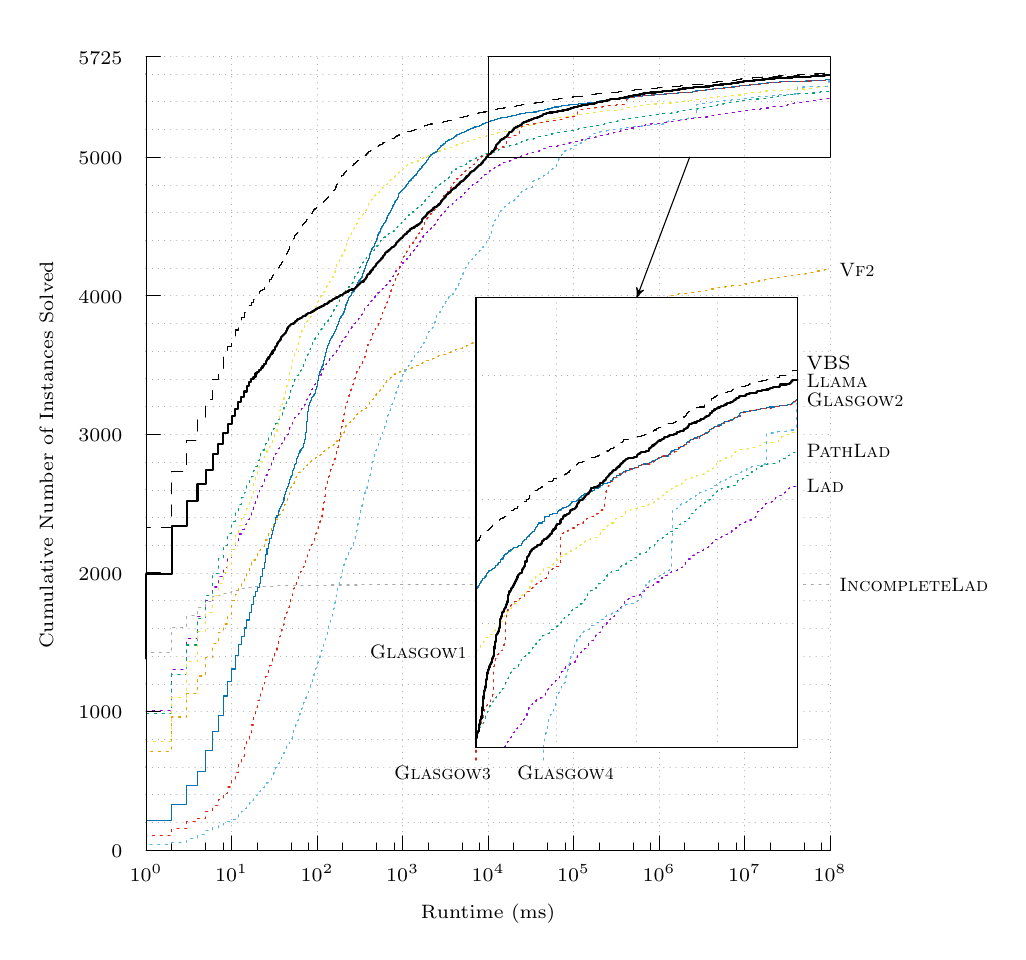
\begin{tikzpicture}[gnuplot]
%% generated with GNUPLOT 5.0p0 (Lua 5.2; terminal rev. 99, script rev. 100)
%% Wed 13 Apr 2016 10:21:36 AEST
\tikzset{every node/.append style={font={\scriptsize}}}
\path (0.000,0.000) rectangle (10.744,11.430);
\gpcolor{color=gp lt color axes}
\gpsetlinetype{gp lt axes}
\gpsetdashtype{gp dt axes}
\gpsetlinewidth{0.50}
\draw[gp path] (1.504,11.061)--(10.191,11.061);
\gpcolor{color=gp lt color border}
\gpsetlinetype{gp lt border}
\gpsetdashtype{gp dt solid}
\gpsetlinewidth{1.00}
\draw[gp path] (1.504,11.061)--(1.684,11.061);
\node[gp node right] at (1.320,11.061) {$5725$};
\gpcolor{color=gp lt color axes}
\gpsetlinetype{gp lt axes}
\gpsetdashtype{gp dt axes}
\gpsetlinewidth{0.50}
\draw[gp path] (1.504,0.985)--(10.191,0.985);
\gpcolor{color=gp lt color border}
\gpsetlinetype{gp lt border}
\gpsetdashtype{gp dt solid}
\gpsetlinewidth{1.00}
\draw[gp path] (1.504,0.985)--(1.684,0.985);
\node[gp node right] at (1.320,0.985) {$0$};
\gpcolor{color=gp lt color axes}
\gpsetlinetype{gp lt axes}
\gpsetdashtype{gp dt axes}
\gpsetlinewidth{0.50}
\draw[gp path] (1.504,1.337)--(10.191,1.337);
\gpcolor{color=gp lt color border}
\gpsetlinetype{gp lt border}
\gpsetdashtype{gp dt solid}
\gpsetlinewidth{1.00}
\draw[gp path] (1.504,1.337)--(1.505,1.337);
\gpcolor{color=gp lt color axes}
\gpsetlinetype{gp lt axes}
\gpsetdashtype{gp dt axes}
\gpsetlinewidth{0.50}
\draw[gp path] (1.504,1.689)--(10.191,1.689);
\gpcolor{color=gp lt color border}
\gpsetlinetype{gp lt border}
\gpsetdashtype{gp dt solid}
\gpsetlinewidth{1.00}
\draw[gp path] (1.504,1.689)--(1.505,1.689);
\gpcolor{color=gp lt color axes}
\gpsetlinetype{gp lt axes}
\gpsetdashtype{gp dt axes}
\gpsetlinewidth{0.50}
\draw[gp path] (1.504,2.041)--(10.191,2.041);
\gpcolor{color=gp lt color border}
\gpsetlinetype{gp lt border}
\gpsetdashtype{gp dt solid}
\gpsetlinewidth{1.00}
\draw[gp path] (1.504,2.041)--(1.505,2.041);
\gpcolor{color=gp lt color axes}
\gpsetlinetype{gp lt axes}
\gpsetdashtype{gp dt axes}
\gpsetlinewidth{0.50}
\draw[gp path] (1.504,2.393)--(10.191,2.393);
\gpcolor{color=gp lt color border}
\gpsetlinetype{gp lt border}
\gpsetdashtype{gp dt solid}
\gpsetlinewidth{1.00}
\draw[gp path] (1.504,2.393)--(1.505,2.393);
\gpcolor{color=gp lt color axes}
\gpsetlinetype{gp lt axes}
\gpsetdashtype{gp dt axes}
\gpsetlinewidth{0.50}
\draw[gp path] (1.504,2.745)--(10.191,2.745);
\gpcolor{color=gp lt color border}
\gpsetlinetype{gp lt border}
\gpsetdashtype{gp dt solid}
\gpsetlinewidth{1.00}
\draw[gp path] (1.504,2.745)--(1.684,2.745);
\node[gp node right] at (1.320,2.745) {$1000$};
\gpcolor{color=gp lt color axes}
\gpsetlinetype{gp lt axes}
\gpsetdashtype{gp dt axes}
\gpsetlinewidth{0.50}
\draw[gp path] (1.504,3.097)--(10.191,3.097);
\gpcolor{color=gp lt color border}
\gpsetlinetype{gp lt border}
\gpsetdashtype{gp dt solid}
\gpsetlinewidth{1.00}
\draw[gp path] (1.504,3.097)--(1.505,3.097);
\gpcolor{color=gp lt color axes}
\gpsetlinetype{gp lt axes}
\gpsetdashtype{gp dt axes}
\gpsetlinewidth{0.50}
\draw[gp path] (1.504,3.449)--(10.191,3.449);
\gpcolor{color=gp lt color border}
\gpsetlinetype{gp lt border}
\gpsetdashtype{gp dt solid}
\gpsetlinewidth{1.00}
\draw[gp path] (1.504,3.449)--(1.505,3.449);
\gpcolor{color=gp lt color axes}
\gpsetlinetype{gp lt axes}
\gpsetdashtype{gp dt axes}
\gpsetlinewidth{0.50}
\draw[gp path] (1.504,3.801)--(10.191,3.801);
\gpcolor{color=gp lt color border}
\gpsetlinetype{gp lt border}
\gpsetdashtype{gp dt solid}
\gpsetlinewidth{1.00}
\draw[gp path] (1.504,3.801)--(1.505,3.801);
\gpcolor{color=gp lt color axes}
\gpsetlinetype{gp lt axes}
\gpsetdashtype{gp dt axes}
\gpsetlinewidth{0.50}
\draw[gp path] (1.504,4.153)--(10.191,4.153);
\gpcolor{color=gp lt color border}
\gpsetlinetype{gp lt border}
\gpsetdashtype{gp dt solid}
\gpsetlinewidth{1.00}
\draw[gp path] (1.504,4.153)--(1.505,4.153);
\gpcolor{color=gp lt color axes}
\gpsetlinetype{gp lt axes}
\gpsetdashtype{gp dt axes}
\gpsetlinewidth{0.50}
\draw[gp path] (1.504,4.505)--(10.191,4.505);
\gpcolor{color=gp lt color border}
\gpsetlinetype{gp lt border}
\gpsetdashtype{gp dt solid}
\gpsetlinewidth{1.00}
\draw[gp path] (1.504,4.505)--(1.684,4.505);
\node[gp node right] at (1.320,4.505) {$2000$};
\gpcolor{color=gp lt color axes}
\gpsetlinetype{gp lt axes}
\gpsetdashtype{gp dt axes}
\gpsetlinewidth{0.50}
\draw[gp path] (1.504,4.857)--(10.191,4.857);
\gpcolor{color=gp lt color border}
\gpsetlinetype{gp lt border}
\gpsetdashtype{gp dt solid}
\gpsetlinewidth{1.00}
\draw[gp path] (1.504,4.857)--(1.505,4.857);
\gpcolor{color=gp lt color axes}
\gpsetlinetype{gp lt axes}
\gpsetdashtype{gp dt axes}
\gpsetlinewidth{0.50}
\draw[gp path] (1.504,5.209)--(10.191,5.209);
\gpcolor{color=gp lt color border}
\gpsetlinetype{gp lt border}
\gpsetdashtype{gp dt solid}
\gpsetlinewidth{1.00}
\draw[gp path] (1.504,5.209)--(1.505,5.209);
\gpcolor{color=gp lt color axes}
\gpsetlinetype{gp lt axes}
\gpsetdashtype{gp dt axes}
\gpsetlinewidth{0.50}
\draw[gp path] (1.504,5.561)--(10.191,5.561);
\gpcolor{color=gp lt color border}
\gpsetlinetype{gp lt border}
\gpsetdashtype{gp dt solid}
\gpsetlinewidth{1.00}
\draw[gp path] (1.504,5.561)--(1.505,5.561);
\gpcolor{color=gp lt color axes}
\gpsetlinetype{gp lt axes}
\gpsetdashtype{gp dt axes}
\gpsetlinewidth{0.50}
\draw[gp path] (1.504,5.913)--(10.191,5.913);
\gpcolor{color=gp lt color border}
\gpsetlinetype{gp lt border}
\gpsetdashtype{gp dt solid}
\gpsetlinewidth{1.00}
\draw[gp path] (1.504,5.913)--(1.505,5.913);
\gpcolor{color=gp lt color axes}
\gpsetlinetype{gp lt axes}
\gpsetdashtype{gp dt axes}
\gpsetlinewidth{0.50}
\draw[gp path] (1.504,6.265)--(10.191,6.265);
\gpcolor{color=gp lt color border}
\gpsetlinetype{gp lt border}
\gpsetdashtype{gp dt solid}
\gpsetlinewidth{1.00}
\draw[gp path] (1.504,6.265)--(1.684,6.265);
\node[gp node right] at (1.320,6.265) {$3000$};
\gpcolor{color=gp lt color axes}
\gpsetlinetype{gp lt axes}
\gpsetdashtype{gp dt axes}
\gpsetlinewidth{0.50}
\draw[gp path] (1.504,6.617)--(10.191,6.617);
\gpcolor{color=gp lt color border}
\gpsetlinetype{gp lt border}
\gpsetdashtype{gp dt solid}
\gpsetlinewidth{1.00}
\draw[gp path] (1.504,6.617)--(1.505,6.617);
\gpcolor{color=gp lt color axes}
\gpsetlinetype{gp lt axes}
\gpsetdashtype{gp dt axes}
\gpsetlinewidth{0.50}
\draw[gp path] (1.504,6.969)--(10.191,6.969);
\gpcolor{color=gp lt color border}
\gpsetlinetype{gp lt border}
\gpsetdashtype{gp dt solid}
\gpsetlinewidth{1.00}
\draw[gp path] (1.504,6.969)--(1.505,6.969);
\gpcolor{color=gp lt color axes}
\gpsetlinetype{gp lt axes}
\gpsetdashtype{gp dt axes}
\gpsetlinewidth{0.50}
\draw[gp path] (1.504,7.321)--(10.191,7.321);
\gpcolor{color=gp lt color border}
\gpsetlinetype{gp lt border}
\gpsetdashtype{gp dt solid}
\gpsetlinewidth{1.00}
\draw[gp path] (1.504,7.321)--(1.505,7.321);
\gpcolor{color=gp lt color axes}
\gpsetlinetype{gp lt axes}
\gpsetdashtype{gp dt axes}
\gpsetlinewidth{0.50}
\draw[gp path] (1.504,7.673)--(10.191,7.673);
\gpcolor{color=gp lt color border}
\gpsetlinetype{gp lt border}
\gpsetdashtype{gp dt solid}
\gpsetlinewidth{1.00}
\draw[gp path] (1.504,7.673)--(1.505,7.673);
\gpcolor{color=gp lt color axes}
\gpsetlinetype{gp lt axes}
\gpsetdashtype{gp dt axes}
\gpsetlinewidth{0.50}
\draw[gp path] (1.504,8.025)--(10.191,8.025);
\gpcolor{color=gp lt color border}
\gpsetlinetype{gp lt border}
\gpsetdashtype{gp dt solid}
\gpsetlinewidth{1.00}
\draw[gp path] (1.504,8.025)--(1.684,8.025);
\node[gp node right] at (1.320,8.025) {$4000$};
\gpcolor{color=gp lt color axes}
\gpsetlinetype{gp lt axes}
\gpsetdashtype{gp dt axes}
\gpsetlinewidth{0.50}
\draw[gp path] (1.504,8.377)--(10.191,8.377);
\gpcolor{color=gp lt color border}
\gpsetlinetype{gp lt border}
\gpsetdashtype{gp dt solid}
\gpsetlinewidth{1.00}
\draw[gp path] (1.504,8.377)--(1.505,8.377);
\gpcolor{color=gp lt color axes}
\gpsetlinetype{gp lt axes}
\gpsetdashtype{gp dt axes}
\gpsetlinewidth{0.50}
\draw[gp path] (1.504,8.729)--(10.191,8.729);
\gpcolor{color=gp lt color border}
\gpsetlinetype{gp lt border}
\gpsetdashtype{gp dt solid}
\gpsetlinewidth{1.00}
\draw[gp path] (1.504,8.729)--(1.505,8.729);
\gpcolor{color=gp lt color axes}
\gpsetlinetype{gp lt axes}
\gpsetdashtype{gp dt axes}
\gpsetlinewidth{0.50}
\draw[gp path] (1.504,9.081)--(10.191,9.081);
\gpcolor{color=gp lt color border}
\gpsetlinetype{gp lt border}
\gpsetdashtype{gp dt solid}
\gpsetlinewidth{1.00}
\draw[gp path] (1.504,9.081)--(1.505,9.081);
\gpcolor{color=gp lt color axes}
\gpsetlinetype{gp lt axes}
\gpsetdashtype{gp dt axes}
\gpsetlinewidth{0.50}
\draw[gp path] (1.504,9.433)--(10.191,9.433);
\gpcolor{color=gp lt color border}
\gpsetlinetype{gp lt border}
\gpsetdashtype{gp dt solid}
\gpsetlinewidth{1.00}
\draw[gp path] (1.504,9.433)--(1.505,9.433);
\gpcolor{color=gp lt color axes}
\gpsetlinetype{gp lt axes}
\gpsetdashtype{gp dt axes}
\gpsetlinewidth{0.50}
\draw[gp path] (1.504,9.785)--(10.191,9.785);
\gpcolor{color=gp lt color border}
\gpsetlinetype{gp lt border}
\gpsetdashtype{gp dt solid}
\gpsetlinewidth{1.00}
\draw[gp path] (1.504,9.785)--(1.684,9.785);
\node[gp node right] at (1.320,9.785) {$5000$};
\gpcolor{color=gp lt color axes}
\gpsetlinetype{gp lt axes}
\gpsetdashtype{gp dt axes}
\gpsetlinewidth{0.50}
\draw[gp path] (1.504,10.137)--(10.191,10.137);
\gpcolor{color=gp lt color border}
\gpsetlinetype{gp lt border}
\gpsetdashtype{gp dt solid}
\gpsetlinewidth{1.00}
\draw[gp path] (1.504,10.137)--(1.505,10.137);
\gpcolor{color=gp lt color axes}
\gpsetlinetype{gp lt axes}
\gpsetdashtype{gp dt axes}
\gpsetlinewidth{0.50}
\draw[gp path] (1.504,10.489)--(10.191,10.489);
\gpcolor{color=gp lt color border}
\gpsetlinetype{gp lt border}
\gpsetdashtype{gp dt solid}
\gpsetlinewidth{1.00}
\draw[gp path] (1.504,10.489)--(1.505,10.489);
\gpcolor{color=gp lt color axes}
\gpsetlinetype{gp lt axes}
\gpsetdashtype{gp dt axes}
\gpsetlinewidth{0.50}
\draw[gp path] (1.504,10.841)--(10.191,10.841);
\gpcolor{color=gp lt color border}
\gpsetlinetype{gp lt border}
\gpsetdashtype{gp dt solid}
\gpsetlinewidth{1.00}
\draw[gp path] (1.504,10.841)--(1.505,10.841);
\gpcolor{color=gp lt color axes}
\gpsetlinetype{gp lt axes}
\gpsetdashtype{gp dt axes}
\gpsetlinewidth{0.50}
\draw[gp path] (1.504,0.985)--(1.504,11.061);
\gpcolor{color=gp lt color border}
\gpsetlinetype{gp lt border}
\gpsetdashtype{gp dt solid}
\gpsetlinewidth{1.00}
\draw[gp path] (1.504,0.985)--(1.504,1.165);
\node[gp node center] at (1.504,0.677) {$10^{0}$};
\draw[gp path] (1.831,0.985)--(1.831,1.075);
\draw[gp path] (2.263,0.985)--(2.263,1.075);
\draw[gp path] (2.485,0.985)--(2.485,1.075);
\gpcolor{color=gp lt color axes}
\gpsetlinetype{gp lt axes}
\gpsetdashtype{gp dt axes}
\gpsetlinewidth{0.50}
\draw[gp path] (2.590,0.985)--(2.590,11.061);
\gpcolor{color=gp lt color border}
\gpsetlinetype{gp lt border}
\gpsetdashtype{gp dt solid}
\gpsetlinewidth{1.00}
\draw[gp path] (2.590,0.985)--(2.590,1.165);
\node[gp node center] at (2.590,0.677) {$10^{1}$};
\draw[gp path] (2.917,0.985)--(2.917,1.075);
\draw[gp path] (3.349,0.985)--(3.349,1.075);
\draw[gp path] (3.571,0.985)--(3.571,1.075);
\gpcolor{color=gp lt color axes}
\gpsetlinetype{gp lt axes}
\gpsetdashtype{gp dt axes}
\gpsetlinewidth{0.50}
\draw[gp path] (3.676,0.985)--(3.676,11.061);
\gpcolor{color=gp lt color border}
\gpsetlinetype{gp lt border}
\gpsetdashtype{gp dt solid}
\gpsetlinewidth{1.00}
\draw[gp path] (3.676,0.985)--(3.676,1.165);
\node[gp node center] at (3.676,0.677) {$10^{2}$};
\draw[gp path] (4.003,0.985)--(4.003,1.075);
\draw[gp path] (4.435,0.985)--(4.435,1.075);
\draw[gp path] (4.656,0.985)--(4.656,1.075);
\gpcolor{color=gp lt color axes}
\gpsetlinetype{gp lt axes}
\gpsetdashtype{gp dt axes}
\gpsetlinewidth{0.50}
\draw[gp path] (4.762,0.985)--(4.762,11.061);
\gpcolor{color=gp lt color border}
\gpsetlinetype{gp lt border}
\gpsetdashtype{gp dt solid}
\gpsetlinewidth{1.00}
\draw[gp path] (4.762,0.985)--(4.762,1.165);
\node[gp node center] at (4.762,0.677) {$10^{3}$};
\draw[gp path] (5.089,0.985)--(5.089,1.075);
\draw[gp path] (5.521,0.985)--(5.521,1.075);
\draw[gp path] (5.742,0.985)--(5.742,1.075);
\gpcolor{color=gp lt color axes}
\gpsetlinetype{gp lt axes}
\gpsetdashtype{gp dt axes}
\gpsetlinewidth{0.50}
\draw[gp path] (5.848,0.985)--(5.848,11.061);
\gpcolor{color=gp lt color border}
\gpsetlinetype{gp lt border}
\gpsetdashtype{gp dt solid}
\gpsetlinewidth{1.00}
\draw[gp path] (5.848,0.985)--(5.848,1.165);
\node[gp node center] at (5.848,0.677) {$10^{4}$};
\draw[gp path] (6.174,0.985)--(6.174,1.075);
\draw[gp path] (6.606,0.985)--(6.606,1.075);
\draw[gp path] (6.828,0.985)--(6.828,1.075);
\gpcolor{color=gp lt color axes}
\gpsetlinetype{gp lt axes}
\gpsetdashtype{gp dt axes}
\gpsetlinewidth{0.50}
\draw[gp path] (6.933,0.985)--(6.933,11.061);
\gpcolor{color=gp lt color border}
\gpsetlinetype{gp lt border}
\gpsetdashtype{gp dt solid}
\gpsetlinewidth{1.00}
\draw[gp path] (6.933,0.985)--(6.933,1.165);
\node[gp node center] at (6.933,0.677) {$10^{5}$};
\draw[gp path] (7.260,0.985)--(7.260,1.075);
\draw[gp path] (7.692,0.985)--(7.692,1.075);
\draw[gp path] (7.914,0.985)--(7.914,1.075);
\gpcolor{color=gp lt color axes}
\gpsetlinetype{gp lt axes}
\gpsetdashtype{gp dt axes}
\gpsetlinewidth{0.50}
\draw[gp path] (8.019,0.985)--(8.019,11.061);
\gpcolor{color=gp lt color border}
\gpsetlinetype{gp lt border}
\gpsetdashtype{gp dt solid}
\gpsetlinewidth{1.00}
\draw[gp path] (8.019,0.985)--(8.019,1.165);
\node[gp node center] at (8.019,0.677) {$10^{6}$};
\draw[gp path] (8.346,0.985)--(8.346,1.075);
\draw[gp path] (8.778,0.985)--(8.778,1.075);
\draw[gp path] (9.000,0.985)--(9.000,1.075);
\gpcolor{color=gp lt color axes}
\gpsetlinetype{gp lt axes}
\gpsetdashtype{gp dt axes}
\gpsetlinewidth{0.50}
\draw[gp path] (9.105,0.985)--(9.105,11.061);
\gpcolor{color=gp lt color border}
\gpsetlinetype{gp lt border}
\gpsetdashtype{gp dt solid}
\gpsetlinewidth{1.00}
\draw[gp path] (9.105,0.985)--(9.105,1.165);
\node[gp node center] at (9.105,0.677) {$10^{7}$};
\draw[gp path] (9.432,0.985)--(9.432,1.075);
\draw[gp path] (9.864,0.985)--(9.864,1.075);
\draw[gp path] (10.086,0.985)--(10.086,1.075);
\gpcolor{color=gp lt color axes}
\gpsetlinetype{gp lt axes}
\gpsetdashtype{gp dt axes}
\gpsetlinewidth{0.50}
\draw[gp path] (10.191,0.985)--(10.191,11.061);
\gpcolor{color=gp lt color border}
\gpsetlinetype{gp lt border}
\gpsetdashtype{gp dt solid}
\gpsetlinewidth{1.00}
\draw[gp path] (10.191,0.985)--(10.191,1.165);
\node[gp node center] at (10.191,0.677) {$10^{8}$};
\draw[gp path] (1.504,11.061)--(1.504,0.985)--(10.191,0.985);
\node[gp node center,rotate=-270] at (0.246,6.023) {Cumulative Number of Instances Solved};
\node[gp node center] at (5.847,0.215) {Runtime (ms)};
\gpcolor{rgb color={0.580,0.000,0.827}}
\gpsetdashtype{dash pattern=on 2.00*\gpdashlength off 5.00*\gpdashlength }
\draw[gp path] (1.504,2.148)--(1.504,2.757)--(1.831,2.757)--(1.831,3.282)--(2.022,3.282)%
  --(2.022,3.676)--(2.158,3.676)--(2.158,3.952)--(2.263,3.952)--(2.263,4.155)--(2.349,4.155)%
  --(2.349,4.327)--(2.422,4.327)--(2.422,4.457)--(2.485,4.457)--(2.485,4.570)--(2.540,4.570)%
  --(2.540,4.683)--(2.590,4.683)--(2.590,4.799)--(2.635,4.799)--(2.635,4.899)--(2.676,4.899)%
  --(2.676,5.000)--(2.714,5.000)--(2.714,5.059)--(2.749,5.059)--(2.749,5.116)--(2.781,5.116)%
  --(2.781,5.181)--(2.812,5.181)--(2.812,5.235)--(2.840,5.235)--(2.840,5.316)--(2.867,5.316)%
  --(2.867,5.390)--(2.893,5.390)--(2.893,5.448)--(2.917,5.448)--(2.917,5.506)--(2.940,5.506)%
  --(2.940,5.556)--(2.962,5.556)--(2.962,5.607)--(2.983,5.607)--(2.983,5.661)--(3.003,5.661)%
  --(3.003,5.705)--(3.022,5.705)--(3.022,5.744)--(3.040,5.744)--(3.040,5.786)--(3.058,5.786)%
  --(3.058,5.821)--(3.075,5.821)--(3.075,5.864)--(3.092,5.864)--(3.092,5.908)--(3.108,5.908)%
  --(3.108,5.939)--(3.123,5.939)--(3.123,5.966)--(3.138,5.966)--(3.138,5.994)--(3.153,5.994)%
  --(3.153,6.027)--(3.167,6.027)--(3.167,6.052)--(3.181,6.052)--(3.181,6.087)--(3.194,6.087)%
  --(3.194,6.112)--(3.207,6.112)--(3.207,6.128)--(3.219,6.128)--(3.219,6.144)--(3.232,6.144)%
  --(3.232,6.161)--(3.244,6.161)--(3.244,6.173)--(3.255,6.173)--(3.255,6.188)--(3.267,6.188)%
  --(3.267,6.219)--(3.278,6.219)--(3.278,6.237)--(3.289,6.237)--(3.289,6.253)--(3.299,6.253)%
  --(3.299,6.263)--(3.310,6.263)--(3.310,6.276)--(3.320,6.276)--(3.320,6.318)--(3.330,6.318)%
  --(3.330,6.349)--(3.339,6.349)--(3.339,6.371)--(3.349,6.371)--(3.349,6.390)--(3.358,6.390)%
  --(3.358,6.413)--(3.367,6.413)--(3.367,6.436)--(3.376,6.436)--(3.376,6.455)--(3.385,6.455)%
  --(3.385,6.462)--(3.394,6.462)--(3.394,6.478)--(3.402,6.478)--(3.402,6.480)--(3.411,6.480)%
  --(3.411,6.489)--(3.419,6.489)--(3.419,6.496)--(3.427,6.496)--(3.427,6.504)--(3.435,6.504)%
  --(3.435,6.517)--(3.443,6.517)--(3.443,6.525)--(3.450,6.525)--(3.450,6.534)--(3.458,6.534)%
  --(3.458,6.547)--(3.465,6.547)--(3.465,6.562)--(3.473,6.562)--(3.473,6.584)--(3.480,6.584)%
  --(3.480,6.589)--(3.487,6.589)--(3.487,6.596)--(3.494,6.596)--(3.494,6.610)--(3.501,6.610)%
  --(3.501,6.617)--(3.508,6.617)--(3.508,6.629)--(3.514,6.629)--(3.514,6.636)--(3.521,6.636)%
  --(3.521,6.647)--(3.527,6.647)--(3.527,6.657)--(3.534,6.657)--(3.534,6.665)--(3.540,6.665)%
  --(3.540,6.689)--(3.546,6.689)--(3.546,6.703)--(3.552,6.703)--(3.552,6.712)--(3.559,6.712)%
  --(3.559,6.723)--(3.565,6.723)--(3.565,6.737)--(3.571,6.737)--(3.571,6.747)--(3.576,6.747)%
  --(3.576,6.765)--(3.582,6.765)--(3.582,6.774)--(3.588,6.774)--(3.588,6.789)--(3.594,6.789)%
  --(3.594,6.805)--(3.599,6.805)--(3.599,6.816)--(3.605,6.816)--(3.605,6.823)--(3.610,6.823)%
  --(3.610,6.833)--(3.615,6.833)--(3.615,6.844)--(3.621,6.844)--(3.621,6.853)--(3.626,6.853)%
  --(3.626,6.860)--(3.631,6.860)--(3.631,6.869)--(3.636,6.869)--(3.636,6.877)--(3.642,6.877)%
  --(3.642,6.881)--(3.647,6.881)--(3.647,6.899)--(3.652,6.899)--(3.652,6.906)--(3.656,6.906)%
  --(3.656,6.911)--(3.661,6.911)--(3.661,6.914)--(3.666,6.914)--(3.666,6.923)--(3.671,6.923)%
  --(3.671,6.927)--(3.676,6.927)--(3.676,6.932)--(3.680,6.932)--(3.680,6.936)--(3.685,6.936)%
  --(3.685,6.943)--(3.690,6.943)--(3.690,6.950)--(3.694,6.950)--(3.694,6.971)--(3.699,6.971)%
  --(3.699,6.980)--(3.703,6.980)--(3.703,6.987)--(3.708,6.987)--(3.708,6.992)--(3.712,6.992)%
  --(3.712,7.001)--(3.716,7.001)--(3.716,7.004)--(3.721,7.004)--(3.721,7.013)--(3.725,7.013)%
  --(3.725,7.024)--(3.729,7.024)--(3.729,7.043)--(3.733,7.043)--(3.733,7.046)--(3.738,7.046)%
  --(3.738,7.059)--(3.742,7.059)--(3.742,7.071)--(3.746,7.071)--(3.746,7.083)--(3.750,7.083)%
  --(3.750,7.089)--(3.758,7.089)--(3.758,7.099)--(3.762,7.099)--(3.762,7.106)--(3.766,7.106)%
  --(3.766,7.115)--(3.770,7.115)--(3.770,7.124)--(3.773,7.124)--(3.773,7.126)--(3.777,7.126)%
  --(3.777,7.131)--(3.781,7.131)--(3.781,7.140)--(3.785,7.140)--(3.785,7.149)--(3.788,7.149)%
  --(3.788,7.150)--(3.792,7.150)--(3.792,7.159)--(3.796,7.159)--(3.796,7.166)--(3.799,7.166)%
  --(3.799,7.173)--(3.803,7.173)--(3.803,7.177)--(3.807,7.177)--(3.807,7.185)--(3.810,7.185)%
  --(3.810,7.194)--(3.814,7.194)--(3.814,7.196)--(3.817,7.196)--(3.817,7.200)--(3.821,7.200)%
  --(3.821,7.201)--(3.824,7.201)--(3.824,7.205)--(3.828,7.205)--(3.828,7.207)--(3.831,7.207)%
  --(3.831,7.208)--(3.834,7.208)--(3.834,7.217)--(3.838,7.217)--(3.838,7.222)--(3.844,7.222)%
  --(3.844,7.224)--(3.848,7.224)--(3.848,7.229)--(3.851,7.229)--(3.851,7.233)--(3.857,7.233)%
  --(3.857,7.237)--(3.861,7.237)--(3.861,7.244)--(3.867,7.244)--(3.867,7.247)--(3.870,7.247)%
  --(3.870,7.252)--(3.873,7.252)--(3.873,7.258)--(3.876,7.258)--(3.876,7.263)--(3.879,7.263)%
  --(3.879,7.266)--(3.882,7.266)--(3.882,7.268)--(3.885,7.268)--(3.885,7.275)--(3.891,7.275)%
  --(3.891,7.281)--(3.894,7.281)--(3.894,7.286)--(3.900,7.286)--(3.900,7.291)--(3.903,7.291)%
  --(3.903,7.293)--(3.906,7.293)--(3.906,7.295)--(3.909,7.295)--(3.909,7.298)--(3.912,7.298)%
  --(3.912,7.300)--(3.915,7.300)--(3.915,7.303)--(3.918,7.303)--(3.918,7.305)--(3.920,7.305)%
  --(3.920,7.310)--(3.923,7.310)--(3.923,7.317)--(3.926,7.317)--(3.926,7.325)--(3.929,7.325)%
  --(3.929,7.326)--(3.932,7.326)--(3.932,7.328)--(3.934,7.328)--(3.934,7.332)--(3.937,7.332)%
  --(3.937,7.339)--(3.940,7.339)--(3.940,7.347)--(3.942,7.347)--(3.942,7.354)--(3.945,7.354)%
  --(3.945,7.358)--(3.950,7.358)--(3.950,7.361)--(3.953,7.361)--(3.953,7.370)--(3.956,7.370)%
  --(3.956,7.376)--(3.958,7.376)--(3.958,7.383)--(3.961,7.383)--(3.961,7.386)--(3.963,7.386)%
  --(3.963,7.388)--(3.966,7.388)--(3.966,7.390)--(3.968,7.390)--(3.968,7.393)--(3.971,7.393)%
  --(3.971,7.400)--(3.973,7.400)--(3.973,7.404)--(3.976,7.404)--(3.976,7.411)--(3.978,7.411)%
  --(3.978,7.414)--(3.981,7.414)--(3.981,7.420)--(3.983,7.420)--(3.983,7.423)--(3.986,7.423)%
  --(3.986,7.427)--(3.988,7.427)--(3.988,7.430)--(3.991,7.430)--(3.991,7.439)--(3.993,7.439)%
  --(3.993,7.442)--(3.998,7.442)--(3.998,7.448)--(4.000,7.448)--(4.000,7.453)--(4.003,7.453)%
  --(4.003,7.458)--(4.005,7.458)--(4.005,7.465)--(4.007,7.465)--(4.007,7.469)--(4.010,7.469)%
  --(4.010,7.471)--(4.012,7.471)--(4.012,7.474)--(4.017,7.474)--(4.017,7.478)--(4.019,7.478)%
  --(4.019,7.481)--(4.021,7.481)--(4.021,7.483)--(4.023,7.483)--(4.023,7.485)--(4.026,7.485)%
  --(4.026,7.492)--(4.028,7.492)--(4.028,7.493)--(4.030,7.493)--(4.030,7.499)--(4.032,7.499)%
  --(4.032,7.501)--(4.035,7.501)--(4.035,7.504)--(4.039,7.504)--(4.039,7.506)--(4.041,7.506)%
  --(4.041,7.509)--(4.043,7.509)--(4.043,7.511)--(4.045,7.511)--(4.045,7.513)--(4.048,7.513)%
  --(4.048,7.515)--(4.050,7.515)--(4.050,7.522)--(4.054,7.522)--(4.054,7.523)--(4.056,7.523)%
  --(4.056,7.525)--(4.058,7.525)--(4.058,7.532)--(4.060,7.532)--(4.060,7.539)--(4.062,7.539)%
  --(4.062,7.543)--(4.066,7.543)--(4.066,7.548)--(4.069,7.548)--(4.069,7.555)--(4.071,7.555)%
  --(4.071,7.560)--(4.073,7.560)--(4.073,7.566)--(4.075,7.566)--(4.075,7.573)--(4.077,7.573)%
  --(4.077,7.576)--(4.079,7.576)--(4.079,7.581)--(4.081,7.581)--(4.081,7.583)--(4.083,7.583)%
  --(4.083,7.587)--(4.087,7.587)--(4.087,7.590)--(4.089,7.590)--(4.089,7.594)--(4.093,7.594)%
  --(4.093,7.596)--(4.094,7.596)--(4.094,7.599)--(4.096,7.599)--(4.096,7.603)--(4.102,7.603)%
  --(4.102,7.610)--(4.104,7.610)--(4.104,7.611)--(4.106,7.611)--(4.106,7.615)--(4.108,7.615)%
  --(4.108,7.617)--(4.110,7.617)--(4.110,7.620)--(4.112,7.620)--(4.112,7.622)--(4.115,7.622)%
  --(4.115,7.624)--(4.117,7.624)--(4.117,7.625)--(4.119,7.625)--(4.119,7.629)--(4.121,7.629)%
  --(4.121,7.633)--(4.123,7.633)--(4.123,7.634)--(4.126,7.634)--(4.126,7.640)--(4.130,7.640)%
  --(4.130,7.641)--(4.132,7.641)--(4.132,7.645)--(4.134,7.645)--(4.134,7.647)--(4.135,7.647)%
  --(4.135,7.648)--(4.137,7.648)--(4.137,7.650)--(4.139,7.650)--(4.139,7.654)--(4.141,7.654)%
  --(4.141,7.657)--(4.142,7.657)--(4.142,7.664)--(4.144,7.664)--(4.144,7.666)--(4.146,7.666)%
  --(4.146,7.668)--(4.153,7.668)--(4.153,7.671)--(4.156,7.671)--(4.156,7.675)--(4.158,7.675)%
  --(4.158,7.678)--(4.160,7.678)--(4.160,7.680)--(4.161,7.680)--(4.161,7.682)--(4.165,7.682)%
  --(4.165,7.684)--(4.166,7.684)--(4.166,7.685)--(4.168,7.685)--(4.168,7.687)--(4.170,7.687)%
  --(4.170,7.689)--(4.173,7.689)--(4.173,7.691)--(4.178,7.691)--(4.178,7.692)--(4.179,7.692)%
  --(4.179,7.694)--(4.181,7.694)--(4.181,7.698)--(4.184,7.698)--(4.184,7.699)--(4.186,7.699)%
  --(4.186,7.703)--(4.188,7.703)--(4.188,7.705)--(4.191,7.705)--(4.191,7.706)--(4.195,7.706)%
  --(4.195,7.708)--(4.197,7.708)--(4.197,7.712)--(4.199,7.712)--(4.199,7.715)--(4.200,7.715)%
  --(4.200,7.721)--(4.202,7.721)--(4.202,7.722)--(4.203,7.722)--(4.203,7.724)--(4.205,7.724)%
  --(4.205,7.726)--(4.206,7.726)--(4.206,7.731)--(4.208,7.731)--(4.208,7.733)--(4.209,7.733)%
  --(4.209,7.735)--(4.211,7.735)--(4.211,7.740)--(4.215,7.740)--(4.215,7.742)--(4.217,7.742)%
  --(4.217,7.743)--(4.218,7.743)--(4.218,7.745)--(4.220,7.745)--(4.220,7.749)--(4.221,7.749)%
  --(4.221,7.750)--(4.223,7.750)--(4.223,7.752)--(4.224,7.752)--(4.224,7.754)--(4.227,7.754)%
  --(4.227,7.757)--(4.233,7.757)--(4.233,7.759)--(4.236,7.759)--(4.236,7.765)--(4.237,7.765)%
  --(4.237,7.766)--(4.239,7.766)--(4.239,7.768)--(4.240,7.768)--(4.240,7.777)--(4.242,7.777)%
  --(4.242,7.780)--(4.243,7.780)--(4.243,7.784)--(4.246,7.784)--(4.246,7.789)--(4.247,7.789)%
  --(4.247,7.791)--(4.249,7.791)--(4.249,7.794)--(4.250,7.794)--(4.250,7.798)--(4.251,7.798)%
  --(4.251,7.801)--(4.253,7.801)--(4.253,7.805)--(4.254,7.805)--(4.254,7.809)--(4.256,7.809)%
  --(4.256,7.810)--(4.258,7.810)--(4.258,7.812)--(4.260,7.812)--(4.260,7.814)--(4.261,7.814)%
  --(4.261,7.816)--(4.262,7.816)--(4.262,7.819)--(4.264,7.819)--(4.264,7.823)--(4.265,7.823)%
  --(4.265,7.828)--(4.267,7.828)--(4.267,7.831)--(4.268,7.831)--(4.268,7.833)--(4.269,7.833)%
  --(4.269,7.838)--(4.271,7.838)--(4.271,7.840)--(4.272,7.840)--(4.272,7.844)--(4.275,7.844)%
  --(4.275,7.849)--(4.276,7.849)--(4.276,7.851)--(4.277,7.851)--(4.277,7.853)--(4.279,7.853)%
  --(4.279,7.854)--(4.280,7.854)--(4.280,7.858)--(4.281,7.858)--(4.281,7.861)--(4.282,7.861)%
  --(4.282,7.863)--(4.284,7.863)--(4.284,7.865)--(4.286,7.865)--(4.286,7.867)--(4.289,7.867)%
  --(4.289,7.870)--(4.290,7.870)--(4.290,7.875)--(4.291,7.875)--(4.291,7.877)--(4.294,7.877)%
  --(4.294,7.879)--(4.297,7.879)--(4.297,7.881)--(4.298,7.881)--(4.298,7.882)--(4.302,7.882)%
  --(4.302,7.888)--(4.305,7.888)--(4.305,7.889)--(4.310,7.889)--(4.310,7.891)--(4.311,7.891)%
  --(4.311,7.895)--(4.313,7.895)--(4.313,7.900)--(4.314,7.900)--(4.314,7.902)--(4.315,7.902)%
  --(4.315,7.904)--(4.318,7.904)--(4.318,7.905)--(4.321,7.905)--(4.321,7.907)--(4.324,7.907)%
  --(4.324,7.911)--(4.325,7.911)--(4.325,7.914)--(4.330,7.914)--(4.330,7.916)--(4.331,7.916)%
  --(4.331,7.918)--(4.332,7.918)--(4.332,7.919)--(4.337,7.919)--(4.337,7.921)--(4.339,7.921)%
  --(4.339,7.923)--(4.340,7.923)--(4.340,7.925)--(4.345,7.925)--(4.345,7.926)--(4.346,7.926)%
  --(4.346,7.932)--(4.347,7.932)--(4.347,7.933)--(4.348,7.933)--(4.348,7.935)--(4.349,7.935)%
  --(4.349,7.937)--(4.351,7.937)--(4.351,7.941)--(4.353,7.941)--(4.353,7.942)--(4.354,7.942)%
  --(4.354,7.946)--(4.356,7.946)--(4.356,7.948)--(4.357,7.948)--(4.357,7.951)--(4.359,7.951)%
  --(4.359,7.953)--(4.361,7.953)--(4.361,7.955)--(4.363,7.955)--(4.363,7.956)--(4.365,7.956)%
  --(4.365,7.958)--(4.371,7.958)--(4.371,7.962)--(4.373,7.962)--(4.373,7.963)--(4.379,7.963)%
  --(4.379,7.965)--(4.382,7.965)--(4.382,7.969)--(4.384,7.969)--(4.384,7.972)--(4.385,7.972)%
  --(4.385,7.974)--(4.386,7.974)--(4.386,7.976)--(4.388,7.976)--(4.388,7.977)--(4.389,7.977)%
  --(4.389,7.983)--(4.391,7.983)--(4.391,7.985)--(4.393,7.985)--(4.393,7.988)--(4.394,7.988)%
  --(4.394,7.990)--(4.395,7.990)--(4.395,7.992)--(4.400,7.992)--(4.400,7.995)--(4.401,7.995)%
  --(4.401,7.997)--(4.404,7.997)--(4.404,7.999)--(4.406,7.999)--(4.406,8.000)--(4.407,8.000)%
  --(4.407,8.002)--(4.408,8.002)--(4.408,8.004)--(4.409,8.004)--(4.409,8.006)--(4.410,8.006)%
  --(4.410,8.007)--(4.411,8.007)--(4.411,8.011)--(4.412,8.011)--(4.412,8.014)--(4.413,8.014)%
  --(4.413,8.018)--(4.414,8.018)--(4.414,8.020)--(4.415,8.020)--(4.415,8.023)--(4.421,8.023)%
  --(4.421,8.025)--(4.422,8.025)--(4.422,8.027)--(4.423,8.027)--(4.423,8.030)--(4.425,8.030)%
  --(4.425,8.032)--(4.426,8.032)--(4.426,8.036)--(4.431,8.036)--(4.431,8.037)--(4.432,8.037)%
  --(4.432,8.039)--(4.437,8.039)--(4.437,8.043)--(4.439,8.043)--(4.439,8.044)--(4.439,8.046)%
  --(4.441,8.046)--(4.441,8.048)--(4.442,8.048)--(4.442,8.050)--(4.443,8.050)--(4.443,8.051)%
  --(4.444,8.051)--(4.444,8.053)--(4.445,8.053)--(4.445,8.055)--(4.447,8.055)--(4.447,8.057)%
  --(4.448,8.057)--(4.448,8.058)--(4.449,8.058)--(4.449,8.060)--(4.451,8.060)--(4.451,8.062)%
  --(4.455,8.062)--(4.455,8.065)--(4.458,8.065)--(4.458,8.067)--(4.459,8.067)--(4.459,8.069)%
  --(4.463,8.069)--(4.463,8.074)--(4.467,8.074)--(4.467,8.076)--(4.468,8.076)--(4.468,8.078)%
  --(4.469,8.078)--(4.469,8.080)--(4.470,8.080)--(4.470,8.083)--(4.474,8.083)--(4.474,8.085)%
  --(4.481,8.085)--(4.481,8.087)--(4.483,8.087)--(4.483,8.090)--(4.487,8.090)--(4.487,8.092)%
  --(4.490,8.092)--(4.490,8.094)--(4.496,8.094)--(4.496,8.097)--(4.497,8.097)--(4.497,8.101)%
  --(4.499,8.101)--(4.499,8.102)--(4.500,8.102)--(4.500,8.104)--(4.501,8.104)--(4.501,8.106)%
  --(4.503,8.106)--(4.503,8.108)--(4.506,8.108)--(4.506,8.109)--(4.508,8.109)--(4.508,8.113)%
  --(4.514,8.113)--(4.514,8.115)--(4.514,8.117)--(4.516,8.117)--(4.516,8.118)--(4.517,8.118)%
  --(4.517,8.120)--(4.518,8.120)--(4.518,8.124)--(4.520,8.124)--(4.520,8.125)--(4.521,8.125)%
  --(4.521,8.127)--(4.525,8.127)--(4.525,8.129)--(4.525,8.131)--(4.529,8.131)--(4.529,8.132)%
  --(4.530,8.132)--(4.530,8.134)--(4.531,8.134)--(4.531,8.138)--(4.537,8.138)--(4.537,8.139)%
  --(4.538,8.139)--(4.538,8.141)--(4.541,8.141)--(4.541,8.143)--(4.542,8.143)--(4.542,8.150)%
  --(4.544,8.150)--(4.544,8.152)--(4.544,8.153)--(4.547,8.153)--(4.547,8.155)--(4.549,8.155)%
  --(4.549,8.157)--(4.558,8.157)--(4.558,8.159)--(4.559,8.159)--(4.559,8.161)--(4.561,8.161)%
  --(4.561,8.162)--(4.562,8.162)--(4.562,8.164)--(4.564,8.164)--(4.564,8.166)--(4.564,8.168)%
  --(4.566,8.168)--(4.566,8.171)--(4.572,8.171)--(4.572,8.173)--(4.573,8.173)--(4.573,8.175)%
  --(4.573,8.178)--(4.574,8.178)--(4.574,8.180)--(4.576,8.180)--(4.576,8.182)--(4.578,8.182)%
  --(4.578,8.183)--(4.579,8.183)--(4.579,8.185)--(4.581,8.185)--(4.581,8.187)--(4.585,8.187)%
  --(4.585,8.189)--(4.587,8.189)--(4.587,8.190)--(4.587,8.192)--(4.590,8.192)--(4.590,8.194)%
  --(4.593,8.194)--(4.593,8.196)--(4.594,8.196)--(4.594,8.201)--(4.595,8.201)--(4.595,8.205)%
  --(4.595,8.206)--(4.597,8.206)--(4.597,8.208)--(4.598,8.208)--(4.598,8.210)--(4.600,8.210)%
  --(4.600,8.212)--(4.601,8.212)--(4.601,8.213)--(4.605,8.213)--(4.605,8.215)--(4.606,8.215)%
  --(4.606,8.217)--(4.607,8.217)--(4.607,8.219)--(4.607,8.220)--(4.608,8.220)--(4.608,8.222)%
  --(4.611,8.222)--(4.611,8.226)--(4.613,8.226)--(4.613,8.227)--(4.614,8.227)--(4.614,8.231)%
  --(4.615,8.231)--(4.615,8.233)--(4.615,8.234)--(4.616,8.234)--(4.616,8.236)--(4.619,8.236)%
  --(4.619,8.238)--(4.620,8.238)--(4.620,8.240)--(4.621,8.240)--(4.621,8.243)--(4.622,8.243)%
  --(4.622,8.245)--(4.622,8.249)--(4.623,8.249)--(4.623,8.254)--(4.625,8.254)--(4.625,8.256)%
  --(4.627,8.256)--(4.627,8.257)--(4.627,8.263)--(4.628,8.263)--(4.628,8.268)--(4.629,8.268)%
  --(4.629,8.270)--(4.630,8.270)--(4.630,8.271)--(4.640,8.271)--(4.640,8.273)--(4.642,8.273)%
  --(4.642,8.275)--(4.643,8.275)--(4.643,8.277)--(4.644,8.277)--(4.644,8.278)--(4.645,8.278)%
  --(4.645,8.284)--(4.646,8.284)--(4.646,8.287)--(4.647,8.287)--(4.647,8.291)--(4.649,8.291)%
  --(4.649,8.293)--(4.655,8.293)--(4.655,8.294)--(4.656,8.294)--(4.656,8.296)--(4.657,8.296)%
  --(4.657,8.298)--(4.658,8.298)--(4.658,8.300)--(4.659,8.300)--(4.659,8.301)--(4.660,8.301)%
  --(4.660,8.303)--(4.662,8.303)--(4.662,8.307)--(4.663,8.307)--(4.663,8.308)--(4.663,8.312)%
  --(4.665,8.312)--(4.665,8.315)--(4.667,8.315)--(4.667,8.317)--(4.668,8.317)--(4.668,8.319)%
  --(4.669,8.319)--(4.669,8.321)--(4.670,8.321)--(4.670,8.324)--(4.670,8.328)--(4.672,8.328)%
  --(4.672,8.333)--(4.673,8.333)--(4.673,8.337)--(4.674,8.337)--(4.674,8.338)--(4.678,8.338)%
  --(4.678,8.340)--(4.680,8.340)--(4.680,8.342)--(4.688,8.342)--(4.688,8.344)--(4.689,8.344)%
  --(4.689,8.347)--(4.689,8.349)--(4.692,8.349)--(4.692,8.354)--(4.696,8.354)--(4.696,8.356)%
  --(4.698,8.356)--(4.698,8.359)--(4.699,8.359)--(4.699,8.361)--(4.701,8.361)--(4.701,8.363)%
  --(4.702,8.363)--(4.702,8.365)--(4.703,8.365)--(4.703,8.366)--(4.703,8.368)--(4.705,8.368)%
  --(4.705,8.370)--(4.707,8.370)--(4.707,8.373)--(4.717,8.373)--(4.717,8.375)--(4.718,8.375)%
  --(4.718,8.377)--(4.719,8.377)--(4.719,8.379)--(4.723,8.379)--(4.723,8.381)--(4.724,8.381)%
  --(4.724,8.382)--(4.724,8.384)--(4.726,8.384)--(4.726,8.386)--(4.728,8.386)--(4.728,8.388)%
  --(4.728,8.391)--(4.729,8.391)--(4.729,8.393)--(4.730,8.393)--(4.730,8.395)--(4.731,8.395)%
  --(4.731,8.396)--(4.732,8.396)--(4.732,8.398)--(4.734,8.398)--(4.734,8.400)--(4.735,8.400)%
  --(4.735,8.402)--(4.738,8.402)--(4.738,8.403)--(4.741,8.403)--(4.741,8.407)--(4.743,8.407)%
  --(4.743,8.409)--(4.744,8.409)--(4.744,8.410)--(4.746,8.410)--(4.746,8.412)--(4.748,8.412)%
  --(4.748,8.414)--(4.750,8.414)--(4.750,8.416)--(4.753,8.416)--(4.753,8.419)--(4.754,8.419)%
  --(4.754,8.421)--(4.754,8.423)--(4.755,8.423)--(4.755,8.426)--(4.756,8.426)--(4.756,8.428)%
  --(4.756,8.430)--(4.757,8.430)--(4.757,8.432)--(4.760,8.432)--(4.760,8.433)--(4.761,8.433)%
  --(4.761,8.435)--(4.763,8.435)--(4.763,8.437)--(4.766,8.437)--(4.766,8.439)--(4.766,8.442)%
  --(4.771,8.442)--(4.771,8.444)--(4.771,8.447)--(4.774,8.447)--(4.774,8.449)--(4.776,8.449)%
  --(4.776,8.451)--(4.781,8.451)--(4.781,8.453)--(4.782,8.453)--(4.782,8.454)--(4.783,8.454)%
  --(4.783,8.456)--(4.784,8.456)--(4.784,8.458)--(4.784,8.461)--(4.785,8.461)--(4.785,8.463)%
  --(4.785,8.465)--(4.786,8.465)--(4.786,8.470)--(4.788,8.470)--(4.788,8.474)--(4.789,8.474)%
  --(4.789,8.476)--(4.794,8.476)--(4.794,8.477)--(4.798,8.477)--(4.798,8.479)--(4.801,8.479)%
  --(4.801,8.481)--(4.801,8.483)--(4.802,8.483)--(4.802,8.484)--(4.806,8.484)--(4.806,8.486)%
  --(4.809,8.486)--(4.809,8.488)--(4.814,8.488)--(4.814,8.490)--(4.815,8.490)--(4.815,8.491)%
  --(4.818,8.491)--(4.818,8.493)--(4.819,8.493)--(4.819,8.495)--(4.822,8.495)--(4.822,8.498)%
  --(4.823,8.498)--(4.823,8.500)--(4.825,8.500)--(4.825,8.504)--(4.825,8.505)--(4.827,8.505)%
  --(4.827,8.507)--(4.828,8.507)--(4.828,8.509)--(4.829,8.509)--(4.829,8.511)--(4.830,8.511)%
  --(4.830,8.513)--(4.833,8.513)--(4.833,8.514)--(4.834,8.514)--(4.834,8.518)--(4.836,8.518)%
  --(4.836,8.520)--(4.838,8.520)--(4.838,8.523)--(4.839,8.523)--(4.839,8.525)--(4.841,8.525)%
  --(4.841,8.527)--(4.843,8.527)--(4.843,8.528)--(4.844,8.528)--(4.844,8.532)--(4.845,8.532)%
  --(4.845,8.534)--(4.846,8.534)--(4.846,8.535)--(4.846,8.537)--(4.849,8.537)--(4.849,8.539)%
  --(4.852,8.539)--(4.852,8.541)--(4.853,8.541)--(4.853,8.542)--(4.857,8.542)--(4.857,8.546)%
  --(4.858,8.546)--(4.858,8.548)--(4.858,8.549)--(4.858,8.551)--(4.859,8.551)--(4.859,8.553)%
  --(4.860,8.553)--(4.860,8.555)--(4.863,8.555)--(4.863,8.557)--(4.864,8.557)--(4.864,8.558)%
  --(4.864,8.560)--(4.869,8.560)--(4.869,8.562)--(4.870,8.562)--(4.870,8.564)--(4.872,8.564)%
  --(4.872,8.567)--(4.872,8.569)--(4.874,8.569)--(4.874,8.571)--(4.875,8.571)--(4.875,8.572)%
  --(4.881,8.572)--(4.881,8.574)--(4.881,8.576)--(4.885,8.576)--(4.885,8.579)--(4.886,8.579)%
  --(4.886,8.581)--(4.886,8.583)--(4.889,8.583)--(4.889,8.585)--(4.889,8.586)--(4.891,8.586)%
  --(4.891,8.588)--(4.894,8.588)--(4.894,8.590)--(4.895,8.590)--(4.895,8.592)--(4.897,8.592)%
  --(4.897,8.593)--(4.901,8.593)--(4.901,8.595)--(4.903,8.595)--(4.903,8.597)--(4.904,8.597)%
  --(4.904,8.599)--(4.904,8.601)--(4.905,8.601)--(4.905,8.602)--(4.907,8.602)--(4.907,8.606)%
  --(4.907,8.608)--(4.908,8.608)--(4.908,8.611)--(4.910,8.611)--(4.910,8.613)--(4.910,8.615)%
  --(4.911,8.615)--(4.911,8.616)--(4.912,8.616)--(4.912,8.618)--(4.914,8.618)--(4.914,8.620)%
  --(4.915,8.620)--(4.915,8.622)--(4.916,8.622)--(4.916,8.623)--(4.917,8.623)--(4.917,8.625)%
  --(4.918,8.625)--(4.918,8.627)--(4.919,8.627)--(4.919,8.629)--(4.921,8.629)--(4.921,8.630)%
  --(4.924,8.630)--(4.924,8.632)--(4.926,8.632)--(4.926,8.634)--(4.929,8.634)--(4.929,8.636)%
  --(4.930,8.636)--(4.930,8.637)--(4.935,8.637)--(4.935,8.639)--(4.935,8.641)--(4.936,8.641)%
  --(4.936,8.643)--(4.937,8.643)--(4.937,8.645)--(4.941,8.645)--(4.941,8.648)--(4.942,8.648)%
  --(4.942,8.650)--(4.946,8.650)--(4.946,8.652)--(4.948,8.652)--(4.948,8.653)--(4.949,8.653)%
  --(4.949,8.655)--(4.950,8.655)--(4.950,8.657)--(4.952,8.657)--(4.952,8.659)--(4.953,8.659)%
  --(4.953,8.660)--(4.954,8.660)--(4.954,8.664)--(4.956,8.664)--(4.956,8.666)--(4.956,8.667)%
  --(4.960,8.667)--(4.960,8.673)--(4.960,8.674)--(4.962,8.674)--(4.962,8.676)--(4.963,8.676)%
  --(4.963,8.680)--(4.965,8.680)--(4.965,8.683)--(4.967,8.683)--(4.967,8.685)--(4.968,8.685)%
  --(4.968,8.687)--(4.969,8.687)--(4.969,8.689)--(4.970,8.689)--(4.970,8.690)--(4.970,8.692)%
  --(4.970,8.694)--(4.973,8.694)--(4.973,8.699)--(4.974,8.699)--(4.974,8.701)--(4.978,8.701)%
  --(4.978,8.703)--(4.979,8.703)--(4.979,8.704)--(4.980,8.704)--(4.980,8.706)--(4.982,8.706)%
  --(4.982,8.708)--(4.983,8.708)--(4.983,8.710)--(4.984,8.710)--(4.984,8.711)--(4.987,8.711)%
  --(4.987,8.713)--(4.987,8.717)--(4.988,8.717)--(4.988,8.718)--(4.988,8.720)--(4.989,8.720)%
  --(4.989,8.722)--(4.989,8.724)--(4.990,8.724)--(4.990,8.725)--(4.993,8.725)--(4.993,8.727)%
  --(4.993,8.729)--(4.993,8.731)--(4.994,8.731)--(4.994,8.733)--(4.995,8.733)--(4.995,8.734)%
  --(4.996,8.734)--(4.996,8.738)--(4.996,8.740)--(4.997,8.740)--(4.997,8.741)--(4.998,8.741)%
  --(4.998,8.743)--(5.000,8.743)--(5.000,8.745)--(5.007,8.745)--(5.007,8.747)--(5.010,8.747)%
  --(5.010,8.748)--(5.010,8.752)--(5.011,8.752)--(5.011,8.755)--(5.012,8.755)--(5.012,8.757)%
  --(5.013,8.757)--(5.013,8.759)--(5.015,8.759)--(5.015,8.761)--(5.016,8.761)--(5.016,8.762)%
  --(5.016,8.764)--(5.016,8.766)--(5.017,8.766)--(5.017,8.768)--(5.018,8.768)--(5.018,8.769)%
  --(5.020,8.769)--(5.020,8.771)--(5.021,8.771)--(5.021,8.775)--(5.025,8.775)--(5.025,8.777)%
  --(5.027,8.777)--(5.027,8.778)--(5.028,8.778)--(5.028,8.780)--(5.031,8.780)--(5.031,8.782)%
  --(5.031,8.784)--(5.031,8.785)--(5.032,8.785)--(5.032,8.787)--(5.034,8.787)--(5.034,8.789)%
  --(5.034,8.791)--(5.039,8.791)--(5.039,8.792)--(5.043,8.792)--(5.043,8.794)--(5.044,8.794)%
  --(5.044,8.796)--(5.045,8.796)--(5.045,8.798)--(5.045,8.799)--(5.047,8.799)--(5.047,8.801)%
  --(5.049,8.801)--(5.049,8.803)--(5.049,8.808)--(5.050,8.808)--(5.050,8.810)--(5.050,8.812)%
  --(5.053,8.812)--(5.053,8.813)--(5.058,8.813)--(5.058,8.817)--(5.058,8.819)--(5.059,8.819)%
  --(5.059,8.821)--(5.060,8.821)--(5.060,8.822)--(5.061,8.822)--(5.061,8.824)--(5.062,8.824)%
  --(5.062,8.826)--(5.064,8.826)--(5.064,8.829)--(5.073,8.829)--(5.073,8.831)--(5.074,8.831)%
  --(5.074,8.833)--(5.074,8.836)--(5.075,8.836)--(5.075,8.838)--(5.075,8.840)--(5.076,8.840)%
  --(5.076,8.842)--(5.077,8.842)--(5.077,8.843)--(5.081,8.843)--(5.081,8.845)--(5.082,8.845)%
  --(5.082,8.847)--(5.083,8.847)--(5.083,8.849)--(5.083,8.854)--(5.089,8.854)--(5.089,8.857)%
  --(5.092,8.857)--(5.092,8.859)--(5.093,8.859)--(5.093,8.861)--(5.095,8.861)--(5.095,8.863)%
  --(5.098,8.863)--(5.098,8.866)--(5.101,8.866)--(5.101,8.868)--(5.104,8.868)--(5.104,8.870)%
  --(5.105,8.870)--(5.105,8.872)--(5.108,8.872)--(5.108,8.873)--(5.112,8.873)--(5.112,8.875)%
  --(5.114,8.875)--(5.114,8.877)--(5.115,8.877)--(5.115,8.879)--(5.116,8.879)--(5.116,8.880)%
  --(5.118,8.880)--(5.118,8.882)--(5.120,8.882)--(5.120,8.884)--(5.123,8.884)--(5.123,8.886)%
  --(5.125,8.886)--(5.125,8.887)--(5.127,8.887)--(5.127,8.889)--(5.129,8.889)--(5.129,8.891)%
  --(5.130,8.891)--(5.130,8.893)--(5.132,8.893)--(5.132,8.894)--(5.132,8.896)--(5.135,8.896)%
  --(5.135,8.898)--(5.136,8.898)--(5.136,8.901)--(5.136,8.903)--(5.137,8.903)--(5.137,8.905)%
  --(5.137,8.907)--(5.140,8.907)--(5.140,8.910)--(5.143,8.910)--(5.143,8.914)--(5.151,8.914)%
  --(5.151,8.916)--(5.151,8.917)--(5.152,8.917)--(5.152,8.919)--(5.153,8.919)--(5.153,8.921)%
  --(5.157,8.921)--(5.157,8.923)--(5.161,8.923)--(5.161,8.924)--(5.164,8.924)--(5.164,8.926)%
  --(5.165,8.926)--(5.165,8.928)--(5.166,8.928)--(5.166,8.930)--(5.166,8.931)--(5.170,8.931)%
  --(5.170,8.933)--(5.171,8.933)--(5.171,8.935)--(5.175,8.935)--(5.175,8.937)--(5.176,8.937)%
  --(5.176,8.940)--(5.177,8.940)--(5.177,8.942)--(5.180,8.942)--(5.180,8.944)--(5.180,8.945)%
  --(5.184,8.945)--(5.184,8.949)--(5.185,8.949)--(5.185,8.951)--(5.186,8.951)--(5.186,8.953)%
  --(5.187,8.953)--(5.187,8.954)--(5.188,8.954)--(5.188,8.956)--(5.188,8.958)--(5.189,8.958)%
  --(5.189,8.960)--(5.190,8.960)--(5.190,8.963)--(5.190,8.965)--(5.192,8.965)--(5.192,8.967)%
  --(5.193,8.967)--(5.193,8.968)--(5.193,8.970)--(5.194,8.970)--(5.194,8.972)--(5.195,8.972)%
  --(5.195,8.974)--(5.200,8.974)--(5.200,8.977)--(5.201,8.977)--(5.201,8.979)--(5.203,8.979)%
  --(5.203,8.981)--(5.205,8.981)--(5.205,8.982)--(5.207,8.982)--(5.207,8.984)--(5.207,8.986)%
  --(5.208,8.986)--(5.208,8.988)--(5.211,8.988)--(5.211,8.989)--(5.214,8.989)--(5.214,8.991)%
  --(5.214,8.993)--(5.215,8.993)--(5.215,8.995)--(5.216,8.995)--(5.216,8.997)--(5.217,8.997)%
  --(5.217,8.998)--(5.217,9.002)--(5.218,9.002)--(5.218,9.004)--(5.218,9.005)--(5.219,9.005)%
  --(5.219,9.007)--(5.219,9.009)--(5.221,9.009)--(5.221,9.011)--(5.222,9.011)--(5.222,9.012)%
  --(5.222,9.014)--(5.223,9.014)--(5.223,9.018)--(5.224,9.018)--(5.224,9.019)--(5.225,9.019)%
  --(5.225,9.021)--(5.226,9.021)--(5.226,9.023)--(5.229,9.023)--(5.229,9.025)--(5.230,9.025)%
  --(5.230,9.026)--(5.232,9.026)--(5.232,9.028)--(5.234,9.028)--(5.234,9.030)--(5.236,9.030)%
  --(5.236,9.032)--(5.236,9.033)--(5.238,9.033)--(5.238,9.035)--(5.239,9.035)--(5.239,9.037)%
  --(5.242,9.037)--(5.242,9.039)--(5.247,9.039)--(5.247,9.041)--(5.250,9.041)--(5.250,9.042)%
  --(5.251,9.042)--(5.251,9.044)--(5.252,9.044)--(5.252,9.046)--(5.255,9.046)--(5.255,9.048)%
  --(5.256,9.048)--(5.256,9.049)--(5.257,9.049)--(5.257,9.051)--(5.261,9.051)--(5.261,9.053)%
  --(5.262,9.053)--(5.262,9.055)--(5.263,9.055)--(5.263,9.056)--(5.263,9.058)--(5.264,9.058)%
  --(5.264,9.060)--(5.265,9.060)--(5.265,9.062)--(5.270,9.062)--(5.270,9.063)--(5.270,9.065)%
  --(5.273,9.065)--(5.273,9.067)--(5.275,9.067)--(5.275,9.069)--(5.275,9.070)--(5.276,9.070)%
  --(5.276,9.072)--(5.276,9.074)--(5.277,9.074)--(5.277,9.076)--(5.278,9.076)--(5.278,9.077)%
  --(5.284,9.077)--(5.284,9.079)--(5.284,9.081)--(5.286,9.081)--(5.286,9.083)--(5.288,9.083)%
  --(5.288,9.085)--(5.289,9.085)--(5.289,9.086)--(5.291,9.086)--(5.291,9.090)--(5.292,9.090)%
  --(5.292,9.093)--(5.295,9.093)--(5.295,9.097)--(5.297,9.097)--(5.297,9.099)--(5.301,9.099)%
  --(5.301,9.100)--(5.301,9.102)--(5.307,9.102)--(5.307,9.104)--(5.308,9.104)--(5.308,9.106)%
  --(5.311,9.106)--(5.311,9.107)--(5.314,9.107)--(5.314,9.109)--(5.315,9.109)--(5.315,9.111)%
  --(5.315,9.113)--(5.319,9.113)--(5.319,9.114)--(5.322,9.114)--(5.322,9.116)--(5.322,9.118)%
  --(5.323,9.118)--(5.323,9.120)--(5.324,9.120)--(5.324,9.121)--(5.326,9.121)--(5.326,9.123)%
  --(5.326,9.125)--(5.327,9.125)--(5.327,9.127)--(5.327,9.129)--(5.331,9.129)--(5.331,9.132)%
  --(5.331,9.134)--(5.332,9.134)--(5.332,9.136)--(5.333,9.136)--(5.333,9.137)--(5.334,9.137)%
  --(5.334,9.139)--(5.335,9.139)--(5.335,9.141)--(5.336,9.141)--(5.336,9.143)--(5.338,9.143)%
  --(5.338,9.144)--(5.338,9.146)--(5.339,9.146)--(5.339,9.148)--(5.340,9.148)--(5.340,9.150)%
  --(5.341,9.150)--(5.341,9.151)--(5.342,9.151)--(5.342,9.153)--(5.343,9.153)--(5.343,9.155)%
  --(5.344,9.155)--(5.344,9.157)--(5.345,9.157)--(5.345,9.158)--(5.345,9.160)--(5.348,9.160)%
  --(5.348,9.162)--(5.354,9.162)--(5.354,9.164)--(5.357,9.164)--(5.357,9.165)--(5.358,9.165)%
  --(5.358,9.167)--(5.360,9.167)--(5.360,9.169)--(5.371,9.169)--(5.371,9.171)--(5.372,9.171)%
  --(5.372,9.173)--(5.372,9.174)--(5.375,9.174)--(5.375,9.176)--(5.381,9.176)--(5.381,9.178)%
  --(5.385,9.178)--(5.385,9.180)--(5.385,9.181)--(5.389,9.181)--(5.389,9.183)--(5.390,9.183)%
  --(5.390,9.185)--(5.391,9.185)--(5.391,9.187)--(5.392,9.187)--(5.392,9.188)--(5.392,9.190)%
  --(5.394,9.190)--(5.394,9.192)--(5.395,9.192)--(5.395,9.194)--(5.396,9.194)--(5.396,9.195)%
  --(5.398,9.195)--(5.398,9.197)--(5.399,9.197)--(5.399,9.199)--(5.399,9.201)--(5.399,9.202)%
  --(5.402,9.202)--(5.402,9.204)--(5.402,9.206)--(5.404,9.206)--(5.404,9.208)--(5.405,9.208)%
  --(5.405,9.209)--(5.410,9.209)--(5.410,9.211)--(5.411,9.211)--(5.411,9.213)--(5.416,9.213)%
  --(5.416,9.215)--(5.417,9.215)--(5.417,9.217)--(5.417,9.218)--(5.418,9.218)--(5.418,9.220)%
  --(5.425,9.220)--(5.425,9.222)--(5.426,9.222)--(5.426,9.224)--(5.431,9.224)--(5.431,9.225)%
  --(5.432,9.225)--(5.432,9.227)--(5.432,9.229)--(5.436,9.229)--(5.436,9.231)--(5.438,9.231)%
  --(5.438,9.232)--(5.439,9.232)--(5.439,9.234)--(5.441,9.234)--(5.441,9.238)--(5.442,9.238)%
  --(5.442,9.239)--(5.443,9.239)--(5.443,9.241)--(5.443,9.243)--(5.445,9.243)--(5.445,9.245)%
  --(5.448,9.245)--(5.448,9.246)--(5.448,9.250)--(5.452,9.250)--(5.452,9.252)--(5.453,9.252)%
  --(5.453,9.253)--(5.460,9.253)--(5.460,9.255)--(5.462,9.255)--(5.462,9.257)--(5.463,9.257)%
  --(5.463,9.259)--(5.463,9.261)--(5.464,9.261)--(5.464,9.262)--(5.467,9.262)--(5.467,9.264)%
  --(5.471,9.264)--(5.471,9.266)--(5.477,9.266)--(5.477,9.268)--(5.479,9.268)--(5.479,9.269)%
  --(5.480,9.269)--(5.480,9.271)--(5.484,9.271)--(5.484,9.273)--(5.487,9.273)--(5.487,9.275)%
  --(5.491,9.275)--(5.491,9.276)--(5.496,9.276)--(5.496,9.278)--(5.499,9.278)--(5.499,9.280)%
  --(5.503,9.280)--(5.503,9.282)--(5.511,9.282)--(5.511,9.283)--(5.515,9.283)--(5.515,9.285)%
  --(5.519,9.285)--(5.519,9.287)--(5.520,9.287)--(5.520,9.289)--(5.525,9.289)--(5.525,9.290)%
  --(5.528,9.290)--(5.528,9.292)--(5.531,9.292)--(5.531,9.294)--(5.532,9.294)--(5.532,9.296)%
  --(5.536,9.296)--(5.536,9.297)--(5.537,9.297)--(5.537,9.299)--(5.538,9.299)--(5.538,9.301)%
  --(5.541,9.301)--(5.541,9.303)--(5.541,9.305)--(5.541,9.306)--(5.542,9.306)--(5.542,9.308)%
  --(5.544,9.308)--(5.544,9.310)--(5.544,9.313)--(5.544,9.315)--(5.544,9.317)--(5.545,9.317)%
  --(5.545,9.319)--(5.545,9.320)--(5.545,9.322)--(5.547,9.322)--(5.547,9.324)--(5.547,9.326)%
  --(5.547,9.327)--(5.550,9.327)--(5.550,9.329)--(5.551,9.329)--(5.551,9.331)--(5.552,9.331)%
  --(5.552,9.333)--(5.552,9.334)--(5.554,9.334)--(5.554,9.336)--(5.555,9.336)--(5.555,9.338)%
  --(5.556,9.338)--(5.556,9.340)--(5.557,9.340)--(5.557,9.341)--(5.559,9.341)--(5.559,9.343)%
  --(5.560,9.343)--(5.560,9.345)--(5.560,9.347)--(5.562,9.347)--(5.562,9.349)--(5.562,9.350)%
  --(5.562,9.352)--(5.564,9.352)--(5.564,9.354)--(5.564,9.356)--(5.564,9.357)--(5.568,9.357)%
  --(5.568,9.359)--(5.570,9.359)--(5.570,9.361)--(5.572,9.361)--(5.572,9.363)--(5.573,9.363)%
  --(5.573,9.364)--(5.574,9.364)--(5.574,9.366)--(5.579,9.366)--(5.579,9.368)--(5.582,9.368)%
  --(5.582,9.370)--(5.583,9.370)--(5.583,9.371)--(5.584,9.371)--(5.584,9.373)--(5.588,9.373)%
  --(5.588,9.375)--(5.597,9.375)--(5.597,9.377)--(5.601,9.377)--(5.601,9.378)--(5.602,9.378)%
  --(5.602,9.380)--(5.603,9.380)--(5.603,9.384)--(5.608,9.384)--(5.608,9.385)--(5.610,9.385)%
  --(5.610,9.387)--(5.619,9.387)--(5.619,9.389)--(5.621,9.389)--(5.621,9.391)--(5.623,9.391)%
  --(5.623,9.393)--(5.623,9.394)--(5.624,9.394)--(5.624,9.396)--(5.624,9.398)--(5.626,9.398)%
  --(5.626,9.400)--(5.626,9.401)--(5.630,9.401)--(5.630,9.403)--(5.631,9.403)--(5.631,9.405)%
  --(5.632,9.405)--(5.632,9.407)--(5.635,9.407)--(5.635,9.408)--(5.635,9.410)--(5.636,9.410)%
  --(5.636,9.412)--(5.637,9.412)--(5.637,9.414)--(5.638,9.414)--(5.638,9.415)--(5.638,9.417)%
  --(5.643,9.417)--(5.643,9.419)--(5.644,9.419)--(5.644,9.421)--(5.647,9.421)--(5.647,9.422)%
  --(5.647,9.424)--(5.649,9.424)--(5.649,9.426)--(5.650,9.426)--(5.650,9.428)--(5.650,9.429)%
  --(5.651,9.429)--(5.651,9.431)--(5.652,9.431)--(5.652,9.433)--(5.653,9.433)--(5.653,9.435)%
  --(5.654,9.435)--(5.654,9.437)--(5.663,9.437)--(5.663,9.438)--(5.667,9.438)--(5.667,9.440)%
  --(5.674,9.440)--(5.674,9.442)--(5.676,9.442)--(5.676,9.444)--(5.678,9.444)--(5.678,9.445)%
  --(5.683,9.445)--(5.683,9.447)--(5.685,9.447)--(5.685,9.449)--(5.685,9.451)--(5.686,9.451)%
  --(5.686,9.452)--(5.689,9.452)--(5.689,9.454)--(5.692,9.454)--(5.692,9.456)--(5.694,9.456)%
  --(5.694,9.458)--(5.698,9.458)--(5.698,9.459)--(5.701,9.459)--(5.701,9.461)--(5.704,9.461)%
  --(5.704,9.463)--(5.705,9.463)--(5.705,9.465)--(5.713,9.465)--(5.713,9.466)--(5.714,9.466)%
  --(5.714,9.468)--(5.716,9.468)--(5.716,9.470)--(5.717,9.470)--(5.717,9.472)--(5.719,9.472)%
  --(5.719,9.473)--(5.722,9.473)--(5.722,9.475)--(5.724,9.475)--(5.724,9.477)--(5.725,9.477)%
  --(5.725,9.479)--(5.728,9.479)--(5.728,9.481)--(5.729,9.481)--(5.729,9.482)--(5.732,9.482)%
  --(5.732,9.484)--(5.738,9.484)--(5.738,9.486)--(5.739,9.486)--(5.739,9.488)--(5.739,9.489)%
  --(5.740,9.489)--(5.740,9.491)--(5.742,9.491)--(5.742,9.493)--(5.742,9.495)--(5.742,9.496)%
  --(5.743,9.496)--(5.743,9.498)--(5.749,9.498)--(5.749,9.500)--(5.751,9.500)--(5.751,9.502)%
  --(5.752,9.502)--(5.752,9.503)--(5.752,9.505)--(5.753,9.505)--(5.753,9.507)--(5.754,9.507)%
  --(5.754,9.509)--(5.755,9.509)--(5.755,9.510)--(5.757,9.510)--(5.757,9.512)--(5.758,9.512)%
  --(5.758,9.514)--(5.759,9.514)--(5.759,9.516)--(5.763,9.516)--(5.763,9.517)--(5.763,9.519)%
  --(5.764,9.519)--(5.764,9.521)--(5.765,9.521)--(5.765,9.523)--(5.765,9.525)--(5.768,9.525)%
  --(5.768,9.526)--(5.769,9.526)--(5.769,9.528)--(5.769,9.530)--(5.770,9.530)--(5.770,9.532)%
  --(5.771,9.532)--(5.771,9.533)--(5.773,9.533)--(5.773,9.535)--(5.775,9.535)--(5.775,9.537)%
  --(5.775,9.539)--(5.776,9.539)--(5.776,9.540)--(5.776,9.542)--(5.777,9.542)--(5.777,9.544)%
  --(5.779,9.544)--(5.779,9.546)--(5.780,9.546)--(5.780,9.547)--(5.781,9.547)--(5.781,9.549)%
  --(5.782,9.549)--(5.782,9.551)--(5.787,9.551)--(5.787,9.553)--(5.788,9.553)--(5.788,9.554)%
  --(5.797,9.554)--(5.797,9.556)--(5.799,9.556)--(5.799,9.558)--(5.804,9.558)--(5.804,9.560)%
  --(5.809,9.560)--(5.809,9.561)--(5.817,9.561)--(5.817,9.563)--(5.817,9.565)--(5.824,9.565)%
  --(5.824,9.567)--(5.828,9.567)--(5.828,9.569)--(5.831,9.569)--(5.831,9.570)--(5.832,9.570)%
  --(5.832,9.572)--(5.836,9.572)--(5.836,9.574)--(5.837,9.574)--(5.837,9.576)--(5.839,9.576)%
  --(5.839,9.577)--(5.840,9.577)--(5.840,9.579)--(5.840,9.581)--(5.843,9.581)--(5.843,9.583)%
  --(5.844,9.583)--(5.844,9.584)--(5.844,9.586)--(5.845,9.586)--(5.845,9.588)--(5.848,9.588)%
  --(5.848,9.590)--(5.848,9.591)--(5.849,9.591)--(5.849,9.593)--(5.851,9.593)--(5.851,9.595)%
  --(5.853,9.595)--(5.853,9.597)--(5.863,9.597)--(5.863,9.600)--(5.863,9.602)--(5.864,9.602)%
  --(5.864,9.604)--(5.865,9.604)--(5.865,9.605)--(5.865,9.607)--(5.869,9.607)--(5.869,9.609)%
  --(5.871,9.609)--(5.871,9.611)--(5.872,9.611)--(5.872,9.613)--(5.873,9.613)--(5.873,9.614)%
  --(5.877,9.614)--(5.877,9.616)--(5.877,9.618)--(5.879,9.618)--(5.879,9.620)--(5.879,9.621)%
  --(5.881,9.621)--(5.881,9.623)--(5.885,9.623)--(5.885,9.625)--(5.890,9.625)--(5.890,9.627)%
  --(5.898,9.627)--(5.898,9.628)--(5.902,9.628)--(5.902,9.630)--(5.904,9.630)--(5.904,9.632)%
  --(5.905,9.632)--(5.905,9.634)--(5.906,9.634)--(5.906,9.635)--(5.914,9.635)--(5.914,9.637)%
  --(5.919,9.637)--(5.919,9.639)--(5.922,9.639)--(5.922,9.641)--(5.923,9.641)--(5.923,9.642)%
  --(5.926,9.642)--(5.926,9.644)--(5.927,9.644)--(5.927,9.646)--(5.930,9.646)--(5.930,9.648)%
  --(5.931,9.648)--(5.931,9.649)--(5.935,9.649)--(5.935,9.651)--(5.937,9.651)--(5.937,9.653)%
  --(5.945,9.653)--(5.945,9.655)--(5.947,9.655)--(5.947,9.657)--(5.959,9.657)--(5.959,9.658)%
  --(5.963,9.658)--(5.963,9.660)--(5.967,9.660)--(5.967,9.662)--(5.967,9.664)--(5.968,9.664)%
  --(5.968,9.665)--(5.968,9.667)--(5.970,9.667)--(5.970,9.669)--(5.974,9.669)--(5.974,9.671)%
  --(5.975,9.671)--(5.975,9.672)--(5.982,9.672)--(5.982,9.674)--(5.983,9.674)--(5.983,9.676)%
  --(5.987,9.676)--(5.987,9.678)--(5.988,9.678)--(5.988,9.679)--(5.989,9.679)--(5.989,9.681)%
  --(5.994,9.681)--(5.994,9.683)--(5.996,9.683)--(5.996,9.685)--(5.997,9.685)--(5.997,9.686)%
  --(5.998,9.686)--(5.998,9.688)--(5.999,9.688)--(5.999,9.690)--(6.000,9.690)--(6.000,9.692)%
  --(6.007,9.692)--(6.007,9.693)--(6.010,9.693)--(6.010,9.695)--(6.013,9.695)--(6.013,9.697)%
  --(6.019,9.697)--(6.019,9.699)--(6.026,9.699)--(6.026,9.701)--(6.028,9.701)--(6.028,9.702)%
  --(6.030,9.702)--(6.030,9.704)--(6.032,9.704)--(6.032,9.706)--(6.036,9.706)--(6.036,9.708)%
  --(6.038,9.708)--(6.038,9.709)--(6.039,9.709)--(6.039,9.711)--(6.042,9.711)--(6.042,9.713)%
  --(6.042,9.715)--(6.048,9.715)--(6.048,9.716)--(6.053,9.716)--(6.053,9.718)--(6.054,9.718)%
  --(6.054,9.720)--(6.059,9.720)--(6.059,9.722)--(6.066,9.722)--(6.066,9.723)--(6.075,9.723)%
  --(6.075,9.725)--(6.082,9.725)--(6.082,9.727)--(6.087,9.727)--(6.087,9.729)--(6.088,9.729)%
  --(6.088,9.730)--(6.096,9.730)--(6.096,9.732)--(6.109,9.732)--(6.109,9.734)--(6.110,9.734)%
  --(6.110,9.736)--(6.115,9.736)--(6.115,9.737)--(6.125,9.737)--(6.125,9.739)--(6.128,9.739)%
  --(6.128,9.741)--(6.129,9.741)--(6.129,9.743)--(6.136,9.743)--(6.136,9.745)--(6.143,9.745)%
  --(6.143,9.746)--(6.144,9.746)--(6.144,9.748)--(6.146,9.748)--(6.146,9.750)--(6.156,9.750)%
  --(6.156,9.752)--(6.160,9.752)--(6.160,9.753)--(6.160,9.755)--(6.163,9.755)--(6.163,9.757)%
  --(6.165,9.757)--(6.165,9.759)--(6.165,9.760)--(6.167,9.760)--(6.167,9.762)--(6.173,9.762)%
  --(6.173,9.764)--(6.185,9.764)--(6.185,9.766)--(6.186,9.766)--(6.186,9.767)--(6.187,9.767)%
  --(6.187,9.769)--(6.192,9.769)--(6.192,9.771)--(6.193,9.771)--(6.193,9.773)--(6.196,9.773)%
  --(6.196,9.774)--(6.205,9.774)--(6.205,9.776)--(6.221,9.776)--(6.221,9.778)--(6.222,9.778)%
  --(6.222,9.780)--(6.230,9.780)--(6.230,9.781)--(6.234,9.781)--(6.234,9.783)--(6.237,9.783)%
  --(6.237,9.785)--(6.237,9.787)--(6.239,9.787)--(6.239,9.789)--(6.240,9.789)--(6.240,9.790)%
  --(6.243,9.790)--(6.243,9.792)--(6.246,9.792)--(6.246,9.794)--(6.260,9.794)--(6.260,9.796)%
  --(6.262,9.796)--(6.262,9.797)--(6.264,9.797)--(6.264,9.799)--(6.273,9.799)--(6.273,9.801)%
  --(6.277,9.801)--(6.277,9.803)--(6.305,9.803)--(6.305,9.804)--(6.307,9.804)--(6.307,9.806)%
  --(6.310,9.806)--(6.310,9.808)--(6.310,9.810)--(6.312,9.810)--(6.312,9.811)--(6.314,9.811)%
  --(6.314,9.813)--(6.323,9.813)--(6.323,9.815)--(6.325,9.815)--(6.325,9.817)--(6.328,9.817)%
  --(6.328,9.818)--(6.333,9.818)--(6.333,9.820)--(6.338,9.820)--(6.338,9.822)--(6.340,9.822)%
  --(6.340,9.824)--(6.347,9.824)--(6.347,9.825)--(6.350,9.825)--(6.350,9.827)--(6.360,9.827)%
  --(6.360,9.829)--(6.362,9.829)--(6.362,9.831)--(6.365,9.831)--(6.365,9.833)--(6.373,9.833)%
  --(6.373,9.834)--(6.385,9.834)--(6.385,9.836)--(6.388,9.836)--(6.388,9.838)--(6.401,9.838)%
  --(6.401,9.840)--(6.404,9.840)--(6.404,9.841)--(6.414,9.841)--(6.414,9.843)--(6.418,9.843)%
  --(6.418,9.845)--(6.420,9.845)--(6.420,9.847)--(6.429,9.847)--(6.429,9.848)--(6.439,9.848)%
  --(6.439,9.850)--(6.462,9.850)--(6.462,9.852)--(6.464,9.852)--(6.464,9.854)--(6.469,9.854)%
  --(6.469,9.855)--(6.470,9.855)--(6.470,9.857)--(6.484,9.857)--(6.484,9.859)--(6.489,9.859)%
  --(6.489,9.861)--(6.493,9.861)--(6.493,9.862)--(6.494,9.862)--(6.494,9.864)--(6.497,9.864)%
  --(6.497,9.866)--(6.500,9.866)--(6.500,9.868)--(6.502,9.868)--(6.502,9.869)--(6.509,9.869)%
  --(6.509,9.871)--(6.522,9.871)--(6.522,9.873)--(6.523,9.873)--(6.523,9.875)--(6.531,9.875)%
  --(6.531,9.877)--(6.537,9.877)--(6.537,9.878)--(6.537,9.880)--(6.537,9.882)--(6.541,9.882)%
  --(6.541,9.884)--(6.541,9.885)--(6.543,9.885)--(6.543,9.887)--(6.551,9.887)--(6.551,9.889)%
  --(6.553,9.889)--(6.553,9.891)--(6.557,9.891)--(6.557,9.892)--(6.560,9.892)--(6.560,9.894)%
  --(6.561,9.894)--(6.561,9.896)--(6.561,9.898)--(6.567,9.898)--(6.567,9.899)--(6.577,9.899)%
  --(6.577,9.901)--(6.592,9.901)--(6.592,9.903)--(6.594,9.903)--(6.594,9.905)--(6.595,9.905)%
  --(6.595,9.906)--(6.606,9.906)--(6.606,9.908)--(6.609,9.908)--(6.609,9.910)--(6.619,9.910)%
  --(6.619,9.912)--(6.620,9.912)--(6.620,9.913)--(6.625,9.913)--(6.625,9.915)--(6.625,9.917)%
  --(6.659,9.917)--(6.659,9.919)--(6.663,9.919)--(6.663,9.921)--(6.670,9.921)--(6.670,9.922)%
  --(6.680,9.922)--(6.680,9.924)--(6.703,9.924)--(6.703,9.926)--(6.725,9.926)--(6.725,9.928)%
  --(6.746,9.928)--(6.746,9.929)--(6.768,9.929)--(6.768,9.931)--(6.775,9.931)--(6.775,9.933)%
  --(6.783,9.933)--(6.783,9.935)--(6.786,9.935)--(6.786,9.936)--(6.787,9.936)--(6.787,9.938)%
  --(6.788,9.938)--(6.788,9.940)--(6.789,9.940)--(6.789,9.942)--(6.805,9.942)--(6.805,9.943)%
  --(6.806,9.943)--(6.806,9.945)--(6.815,9.945)--(6.815,9.947)--(6.817,9.947)--(6.817,9.949)%
  --(6.819,9.949)--(6.819,9.950)--(6.823,9.950)--(6.823,9.952)--(6.834,9.952)--(6.834,9.954)%
  --(6.835,9.954)--(6.835,9.956)--(6.839,9.956)--(6.839,9.957)--(6.863,9.957)--(6.863,9.959)%
  --(6.864,9.959)--(6.864,9.961)--(6.865,9.961)--(6.865,9.963)--(6.870,9.963)--(6.870,9.965)%
  --(6.887,9.965)--(6.887,9.966)--(6.905,9.966)--(6.905,9.968)--(6.912,9.968)--(6.912,9.970)%
  --(6.915,9.970)--(6.915,9.972)--(6.918,9.972)--(6.918,9.973)--(6.927,9.973)--(6.927,9.975)%
  --(6.950,9.975)--(6.950,9.977)--(6.950,9.979)--(6.968,9.979)--(6.968,9.980)--(6.968,9.982)%
  --(6.970,9.982)--(6.970,9.984)--(6.978,9.984)--(6.978,9.986)--(6.979,9.986)--(6.979,9.987)%
  --(6.983,9.987)--(6.983,9.989)--(6.991,9.989)--(6.991,9.991)--(6.992,9.991)--(6.992,9.993)%
  --(6.998,9.993)--(6.998,9.994)--(7.000,9.994)--(7.000,9.996)--(7.003,9.996)--(7.003,9.998)%
  --(7.007,9.998)--(7.007,10.000)--(7.027,10.000)--(7.027,10.001)--(7.036,10.001)--(7.036,10.003)%
  --(7.041,10.003)--(7.041,10.005)--(7.042,10.005)--(7.042,10.007)--(7.044,10.007)--(7.044,10.009)%
  --(7.050,10.009)--(7.050,10.010)--(7.051,10.010)--(7.051,10.012)--(7.058,10.012)--(7.058,10.014)%
  --(7.079,10.014)--(7.079,10.016)--(7.087,10.016)--(7.087,10.017)--(7.104,10.017)--(7.104,10.019)%
  --(7.112,10.019)--(7.112,10.021)--(7.120,10.021)--(7.120,10.023)--(7.157,10.023)--(7.157,10.024)%
  --(7.182,10.024)--(7.182,10.026)--(7.182,10.028)--(7.186,10.028)--(7.186,10.030)--(7.187,10.030)%
  --(7.187,10.031)--(7.188,10.031)--(7.188,10.033)--(7.204,10.033)--(7.204,10.035)--(7.205,10.035)%
  --(7.205,10.037)--(7.206,10.037)--(7.206,10.038)--(7.207,10.038)--(7.207,10.040)--(7.210,10.040)%
  --(7.210,10.042)--(7.217,10.042)--(7.217,10.044)--(7.221,10.044)--(7.221,10.045)--(7.221,10.047)%
  --(7.225,10.047)--(7.225,10.049)--(7.229,10.049)--(7.229,10.051)--(7.248,10.051)--(7.248,10.053)%
  --(7.258,10.053)--(7.258,10.054)--(7.264,10.054)--(7.264,10.056)--(7.271,10.056)--(7.271,10.058)%
  --(7.282,10.058)--(7.282,10.060)--(7.290,10.060)--(7.290,10.061)--(7.297,10.061)--(7.297,10.063)%
  --(7.298,10.063)--(7.298,10.065)--(7.317,10.065)--(7.317,10.067)--(7.334,10.067)--(7.334,10.068)%
  --(7.338,10.068)--(7.338,10.070)--(7.351,10.070)--(7.351,10.072)--(7.357,10.072)--(7.357,10.074)%
  --(7.359,10.074)--(7.359,10.075)--(7.367,10.075)--(7.367,10.077)--(7.371,10.077)--(7.371,10.079)%
  --(7.371,10.081)--(7.377,10.081)--(7.377,10.082)--(7.408,10.082)--(7.408,10.084)--(7.412,10.084)%
  --(7.412,10.086)--(7.412,10.088)--(7.424,10.088)--(7.424,10.089)--(7.432,10.089)--(7.432,10.091)%
  --(7.435,10.091)--(7.435,10.093)--(7.441,10.093)--(7.441,10.095)--(7.458,10.095)--(7.458,10.097)%
  --(7.460,10.097)--(7.460,10.098)--(7.463,10.098)--(7.463,10.100)--(7.465,10.100)--(7.465,10.102)%
  --(7.467,10.102)--(7.467,10.104)--(7.468,10.104)--(7.468,10.105)--(7.501,10.105)--(7.501,10.107)%
  --(7.505,10.107)--(7.505,10.109)--(7.505,10.111)--(7.517,10.111)--(7.517,10.112)--(7.531,10.112)%
  --(7.531,10.114)--(7.532,10.114)--(7.532,10.116)--(7.533,10.116)--(7.533,10.118)--(7.539,10.118)%
  --(7.539,10.119)--(7.547,10.119)--(7.547,10.121)--(7.549,10.121)--(7.549,10.123)--(7.552,10.123)%
  --(7.552,10.125)--(7.554,10.125)--(7.554,10.126)--(7.560,10.126)--(7.560,10.128)--(7.572,10.128)%
  --(7.572,10.130)--(7.575,10.130)--(7.575,10.132)--(7.590,10.132)--(7.590,10.133)--(7.595,10.133)%
  --(7.595,10.135)--(7.606,10.135)--(7.606,10.137)--(7.617,10.137)--(7.617,10.139)--(7.623,10.139)%
  --(7.623,10.141)--(7.624,10.141)--(7.624,10.142)--(7.636,10.142)--(7.636,10.144)--(7.637,10.144)%
  --(7.637,10.146)--(7.640,10.146)--(7.640,10.148)--(7.655,10.148)--(7.655,10.149)--(7.664,10.149)%
  --(7.664,10.151)--(7.664,10.153)--(7.665,10.153)--(7.665,10.155)--(7.670,10.155)--(7.670,10.156)%
  --(7.710,10.156)--(7.710,10.158)--(7.716,10.158)--(7.716,10.160)--(7.724,10.160)--(7.724,10.162)%
  --(7.726,10.162)--(7.726,10.163)--(7.729,10.163)--(7.729,10.165)--(7.734,10.165)--(7.734,10.167)%
  --(7.737,10.167)--(7.737,10.169)--(7.741,10.169)--(7.741,10.170)--(7.747,10.170)--(7.747,10.172)%
  --(7.759,10.172)--(7.759,10.174)--(7.773,10.174)--(7.773,10.176)--(7.782,10.176)--(7.782,10.177)%
  --(7.784,10.177)--(7.784,10.179)--(7.786,10.179)--(7.786,10.181)--(7.787,10.181)--(7.787,10.183)%
  --(7.814,10.183)--(7.814,10.185)--(7.821,10.185)--(7.821,10.186)--(7.826,10.186)--(7.826,10.188)%
  --(7.833,10.188)--(7.833,10.190)--(7.842,10.190)--(7.842,10.192)--(7.847,10.192)--(7.847,10.193)%
  --(7.848,10.193)--(7.848,10.195)--(7.850,10.195)--(7.850,10.197)--(7.853,10.197)--(7.853,10.199)%
  --(7.854,10.199)--(7.854,10.200)--(7.857,10.200)--(7.857,10.202)--(7.873,10.202)--(7.873,10.204)%
  --(7.897,10.204)--(7.897,10.206)--(7.902,10.206)--(7.902,10.207)--(7.918,10.207)--(7.918,10.209)%
  --(7.933,10.209)--(7.933,10.211)--(7.954,10.211)--(7.954,10.213)--(7.969,10.213)--(7.969,10.214)%
  --(8.024,10.214)--(8.024,10.216)--(8.062,10.216)--(8.062,10.218)--(8.063,10.218)--(8.063,10.220)%
  --(8.067,10.220)--(8.067,10.221)--(8.070,10.221)--(8.070,10.223)--(8.079,10.223)--(8.079,10.225)%
  --(8.095,10.225)--(8.095,10.227)--(8.105,10.227)--(8.105,10.229)--(8.125,10.229)--(8.125,10.230)%
  --(8.126,10.230)--(8.126,10.232)--(8.130,10.232)--(8.130,10.234)--(8.134,10.234)--(8.134,10.236)%
  --(8.139,10.236)--(8.139,10.237)--(8.150,10.237)--(8.150,10.239)--(8.179,10.239)--(8.179,10.241)%
  --(8.196,10.241)--(8.196,10.243)--(8.233,10.243)--(8.233,10.244)--(8.238,10.244)--(8.238,10.246)%
  --(8.250,10.246)--(8.250,10.248)--(8.254,10.248)--(8.254,10.250)--(8.257,10.250)--(8.257,10.251)%
  --(8.265,10.251)--(8.265,10.253)--(8.267,10.253)--(8.267,10.255)--(8.322,10.255)--(8.322,10.257)%
  --(8.331,10.257)--(8.331,10.258)--(8.341,10.258)--(8.341,10.260)--(8.350,10.260)--(8.350,10.262)%
  --(8.352,10.262)--(8.352,10.264)--(8.359,10.264)--(8.359,10.265)--(8.361,10.265)--(8.361,10.267)%
  --(8.363,10.267)--(8.363,10.269)--(8.377,10.269)--(8.377,10.271)--(8.396,10.271)--(8.396,10.273)%
  --(8.405,10.273)--(8.405,10.274)--(8.434,10.274)--(8.434,10.276)--(8.440,10.276)--(8.440,10.278)%
  --(8.443,10.278)--(8.443,10.280)--(8.472,10.280)--(8.472,10.281)--(8.480,10.281)--(8.480,10.283)%
  --(8.491,10.283)--(8.491,10.285)--(8.492,10.285)--(8.492,10.287)--(8.529,10.287)--(8.529,10.288)%
  --(8.566,10.288)--(8.566,10.290)--(8.591,10.290)--(8.591,10.292)--(8.610,10.292)--(8.610,10.294)%
  --(8.615,10.294)--(8.615,10.295)--(8.631,10.295)--(8.631,10.297)--(8.639,10.297)--(8.639,10.299)%
  --(8.647,10.299)--(8.647,10.301)--(8.654,10.301)--(8.654,10.302)--(8.655,10.302)--(8.655,10.304)%
  --(8.667,10.304)--(8.667,10.306)--(8.677,10.306)--(8.677,10.308)--(8.682,10.308)--(8.682,10.309)%
  --(8.683,10.309)--(8.683,10.311)--(8.683,10.313)--(8.687,10.313)--(8.687,10.315)--(8.710,10.315)%
  --(8.710,10.317)--(8.721,10.317)--(8.721,10.318)--(8.724,10.318)--(8.724,10.320)--(8.745,10.320)%
  --(8.745,10.322)--(8.750,10.322)--(8.750,10.324)--(8.761,10.324)--(8.761,10.325)--(8.763,10.325)%
  --(8.763,10.327)--(8.767,10.327)--(8.767,10.329)--(8.777,10.329)--(8.777,10.331)--(8.793,10.331)%
  --(8.793,10.332)--(8.806,10.332)--(8.806,10.334)--(8.811,10.334)--(8.811,10.336)--(8.844,10.336)%
  --(8.844,10.338)--(8.844,10.339)--(8.873,10.339)--(8.873,10.341)--(8.885,10.341)--(8.885,10.343)%
  --(8.914,10.343)--(8.914,10.345)--(8.916,10.345)--(8.916,10.346)--(8.924,10.346)--(8.924,10.348)%
  --(8.925,10.348)--(8.925,10.350)--(8.945,10.350)--(8.945,10.352)--(8.972,10.352)--(8.972,10.353)%
  --(8.990,10.353)--(8.990,10.355)--(9.005,10.355)--(9.005,10.357)--(9.022,10.357)--(9.022,10.359)%
  --(9.024,10.359)--(9.024,10.361)--(9.033,10.361)--(9.033,10.362)--(9.034,10.362)--(9.034,10.364)%
  --(9.039,10.364)--(9.039,10.366)--(9.050,10.366)--(9.050,10.368)--(9.059,10.368)--(9.059,10.369)%
  --(9.063,10.369)--(9.063,10.371)--(9.068,10.371)--(9.068,10.373)--(9.069,10.373)--(9.069,10.375)%
  --(9.087,10.375)--(9.087,10.376)--(9.128,10.376)--(9.128,10.378)--(9.128,10.380)--(9.137,10.380)%
  --(9.137,10.382)--(9.168,10.382)--(9.168,10.383)--(9.176,10.383)--(9.176,10.385)--(9.179,10.385)%
  --(9.179,10.387)--(9.207,10.387)--(9.207,10.389)--(9.239,10.389)--(9.239,10.390)--(9.241,10.390)%
  --(9.241,10.392)--(9.251,10.392)--(9.251,10.394)--(9.256,10.394)--(9.256,10.396)--(9.304,10.396)%
  --(9.304,10.397)--(9.305,10.397)--(9.305,10.399)--(9.308,10.399)--(9.308,10.401)--(9.333,10.401)%
  --(9.333,10.403)--(9.342,10.403)--(9.342,10.405)--(9.352,10.405)--(9.352,10.406)--(9.354,10.406)%
  --(9.354,10.408)--(9.385,10.408)--(9.385,10.410)--(9.403,10.410)--(9.403,10.412)--(9.408,10.412)%
  --(9.408,10.413)--(9.409,10.413)--(9.409,10.415)--(9.411,10.415)--(9.411,10.417)--(9.426,10.417)%
  --(9.426,10.419)--(9.432,10.419)--(9.432,10.420)--(9.435,10.420)--(9.435,10.422)--(9.437,10.422)%
  --(9.437,10.424)--(9.493,10.424)--(9.493,10.426)--(9.512,10.426)--(9.512,10.427)--(9.531,10.427)%
  --(9.531,10.429)--(9.541,10.429)--(9.541,10.431)--(9.570,10.431)--(9.570,10.433)--(9.595,10.433)%
  --(9.595,10.434)--(9.601,10.434)--(9.601,10.436)--(9.603,10.436)--(9.603,10.438)--(9.618,10.438)%
  --(9.618,10.440)--(9.623,10.440)--(9.623,10.441)--(9.643,10.441)--(9.643,10.443)--(9.645,10.443)%
  --(9.645,10.445)--(9.646,10.445)--(9.646,10.447)--(9.648,10.447)--(9.648,10.449)--(9.651,10.449)%
  --(9.651,10.450)--(9.655,10.450)--(9.655,10.452)--(9.655,10.454)--(9.667,10.454)--(9.667,10.456)%
  --(9.674,10.456)--(9.674,10.457)--(9.675,10.457)--(9.675,10.459)--(9.677,10.459)--(9.677,10.461)%
  --(9.707,10.461)--(9.707,10.463)--(9.710,10.463)--(9.710,10.464)--(9.714,10.464)--(9.714,10.466)%
  --(9.725,10.466)--(9.725,10.468)--(9.727,10.468)--(9.727,10.470)--(9.737,10.470)--(9.737,10.471)%
  --(9.739,10.471)--(9.739,10.473)--(9.759,10.473)--(9.759,10.475)--(9.759,10.477)--(9.782,10.477)%
  --(9.782,10.478)--(9.820,10.478)--(9.820,10.480)--(9.842,10.480)--(9.842,10.482)--(9.856,10.482)%
  --(9.856,10.484)--(9.863,10.484)--(9.863,10.485)--(9.881,10.485)--(9.881,10.487)--(9.881,10.489)%
  --(9.886,10.489)--(9.886,10.491)--(9.890,10.491)--(9.890,10.493)--(9.892,10.493)--(9.892,10.494)%
  --(9.915,10.494)--(9.915,10.496)--(9.924,10.496)--(9.924,10.498)--(9.932,10.498)--(9.932,10.500)%
  --(9.972,10.500)--(9.972,10.501)--(9.994,10.501)--(9.994,10.503)--(10.002,10.503)--(10.002,10.505)%
  --(10.007,10.505)--(10.007,10.507)--(10.021,10.507)--(10.021,10.508)--(10.030,10.508)--(10.030,10.510)%
  --(10.033,10.510)--(10.033,10.512)--(10.038,10.512)--(10.038,10.514)--(10.047,10.514)--(10.047,10.515)%
  --(10.048,10.515)--(10.048,10.517)--(10.069,10.517)--(10.069,10.519)--(10.079,10.519)--(10.079,10.521)%
  --(10.083,10.521)--(10.083,10.522)--(10.123,10.522)--(10.123,10.524)--(10.137,10.524)--(10.137,10.526)%
  --(10.175,10.526)--(10.175,10.528)--(10.191,10.528)--(10.191,10.529);
\gpcolor{rgb color={0.000,0.620,0.451}}
\draw[gp path] (1.504,2.039)--(1.504,2.720)--(1.831,2.720)--(1.831,3.211)--(2.022,3.211)%
  --(2.022,3.590)--(2.158,3.590)--(2.158,3.931)--(2.263,3.931)--(2.263,4.222)--(2.349,4.222)%
  --(2.349,4.496)--(2.422,4.496)--(2.422,4.685)--(2.485,4.685)--(2.485,4.857)--(2.540,4.857)%
  --(2.540,5.010)--(2.590,5.010)--(2.590,5.161)--(2.635,5.161)--(2.635,5.267)--(2.676,5.267)%
  --(2.676,5.374)--(2.714,5.374)--(2.714,5.459)--(2.749,5.459)--(2.749,5.531)--(2.781,5.531)%
  --(2.781,5.616)--(2.812,5.616)--(2.812,5.672)--(2.840,5.672)--(2.840,5.726)--(2.867,5.726)%
  --(2.867,5.807)--(2.893,5.807)--(2.893,5.862)--(2.917,5.862)--(2.917,5.931)--(2.940,5.931)%
  --(2.940,5.982)--(2.962,5.982)--(2.962,6.026)--(2.983,6.026)--(2.983,6.066)--(3.003,6.066)%
  --(3.003,6.096)--(3.022,6.096)--(3.022,6.147)--(3.040,6.147)--(3.040,6.193)--(3.058,6.193)%
  --(3.058,6.223)--(3.075,6.223)--(3.075,6.251)--(3.092,6.251)--(3.092,6.284)--(3.108,6.284)%
  --(3.108,6.318)--(3.123,6.318)--(3.123,6.339)--(3.138,6.339)--(3.138,6.369)--(3.153,6.369)%
  --(3.153,6.399)--(3.167,6.399)--(3.167,6.429)--(3.181,6.429)--(3.181,6.457)--(3.194,6.457)%
  --(3.194,6.476)--(3.207,6.476)--(3.207,6.497)--(3.219,6.497)--(3.219,6.508)--(3.232,6.508)%
  --(3.232,6.536)--(3.244,6.536)--(3.244,6.564)--(3.255,6.564)--(3.255,6.608)--(3.267,6.608)%
  --(3.267,6.635)--(3.278,6.635)--(3.278,6.661)--(3.289,6.661)--(3.289,6.679)--(3.299,6.679)%
  --(3.299,6.701)--(3.310,6.701)--(3.310,6.724)--(3.320,6.724)--(3.320,6.751)--(3.330,6.751)%
  --(3.330,6.788)--(3.339,6.788)--(3.339,6.818)--(3.349,6.818)--(3.349,6.833)--(3.358,6.833)%
  --(3.358,6.851)--(3.367,6.851)--(3.367,6.885)--(3.376,6.885)--(3.376,6.909)--(3.385,6.909)%
  --(3.385,6.937)--(3.394,6.937)--(3.394,6.957)--(3.402,6.957)--(3.402,6.976)--(3.411,6.976)%
  --(3.411,6.992)--(3.419,6.992)--(3.419,7.009)--(3.427,7.009)--(3.427,7.017)--(3.435,7.017)%
  --(3.435,7.031)--(3.443,7.031)--(3.443,7.039)--(3.450,7.039)--(3.450,7.052)--(3.458,7.052)%
  --(3.458,7.064)--(3.465,7.064)--(3.465,7.076)--(3.473,7.076)--(3.473,7.083)--(3.480,7.083)%
  --(3.480,7.096)--(3.487,7.096)--(3.487,7.108)--(3.494,7.108)--(3.494,7.129)--(3.501,7.129)%
  --(3.501,7.150)--(3.508,7.150)--(3.508,7.168)--(3.514,7.168)--(3.514,7.185)--(3.521,7.185)%
  --(3.521,7.193)--(3.527,7.193)--(3.527,7.207)--(3.534,7.207)--(3.534,7.222)--(3.540,7.222)%
  --(3.540,7.240)--(3.546,7.240)--(3.546,7.249)--(3.552,7.249)--(3.552,7.266)--(3.559,7.266)%
  --(3.559,7.281)--(3.565,7.281)--(3.565,7.300)--(3.571,7.300)--(3.571,7.314)--(3.576,7.314)%
  --(3.576,7.326)--(3.582,7.326)--(3.582,7.340)--(3.588,7.340)--(3.588,7.351)--(3.594,7.351)%
  --(3.594,7.365)--(3.599,7.365)--(3.599,7.372)--(3.605,7.372)--(3.605,7.381)--(3.610,7.381)%
  --(3.610,7.398)--(3.615,7.398)--(3.615,7.416)--(3.621,7.416)--(3.621,7.430)--(3.626,7.430)%
  --(3.626,7.448)--(3.631,7.448)--(3.631,7.455)--(3.636,7.455)--(3.636,7.471)--(3.642,7.471)%
  --(3.642,7.474)--(3.647,7.474)--(3.647,7.476)--(3.652,7.476)--(3.652,7.488)--(3.656,7.488)%
  --(3.656,7.499)--(3.661,7.499)--(3.661,7.506)--(3.666,7.506)--(3.666,7.509)--(3.671,7.509)%
  --(3.671,7.511)--(3.676,7.511)--(3.676,7.522)--(3.680,7.522)--(3.680,7.527)--(3.685,7.527)%
  --(3.685,7.529)--(3.690,7.529)--(3.690,7.536)--(3.694,7.536)--(3.694,7.541)--(3.699,7.541)%
  --(3.699,7.552)--(3.703,7.552)--(3.703,7.560)--(3.708,7.560)--(3.708,7.573)--(3.712,7.573)%
  --(3.712,7.580)--(3.716,7.580)--(3.716,7.581)--(3.721,7.581)--(3.721,7.585)--(3.725,7.585)%
  --(3.725,7.596)--(3.729,7.596)--(3.729,7.599)--(3.733,7.599)--(3.733,7.603)--(3.738,7.603)%
  --(3.738,7.610)--(3.742,7.610)--(3.742,7.618)--(3.746,7.618)--(3.746,7.622)--(3.750,7.622)%
  --(3.750,7.625)--(3.754,7.625)--(3.754,7.633)--(3.758,7.633)--(3.758,7.641)--(3.762,7.641)%
  --(3.762,7.647)--(3.766,7.647)--(3.766,7.657)--(3.770,7.657)--(3.770,7.662)--(3.773,7.662)%
  --(3.773,7.668)--(3.777,7.668)--(3.777,7.671)--(3.781,7.671)--(3.781,7.675)--(3.785,7.675)%
  --(3.785,7.677)--(3.792,7.677)--(3.792,7.682)--(3.799,7.682)--(3.799,7.685)--(3.803,7.685)%
  --(3.803,7.691)--(3.807,7.691)--(3.807,7.698)--(3.810,7.698)--(3.810,7.699)--(3.814,7.699)%
  --(3.814,7.705)--(3.817,7.705)--(3.817,7.708)--(3.821,7.708)--(3.821,7.717)--(3.824,7.717)%
  --(3.824,7.722)--(3.828,7.722)--(3.828,7.728)--(3.831,7.728)--(3.831,7.736)--(3.834,7.736)%
  --(3.834,7.740)--(3.838,7.740)--(3.838,7.742)--(3.841,7.742)--(3.841,7.749)--(3.844,7.749)%
  --(3.844,7.752)--(3.848,7.752)--(3.848,7.759)--(3.851,7.759)--(3.851,7.765)--(3.854,7.765)%
  --(3.854,7.768)--(3.857,7.768)--(3.857,7.777)--(3.861,7.777)--(3.861,7.782)--(3.864,7.782)%
  --(3.864,7.787)--(3.867,7.787)--(3.867,7.791)--(3.870,7.791)--(3.870,7.798)--(3.873,7.798)%
  --(3.873,7.805)--(3.876,7.805)--(3.876,7.810)--(3.879,7.810)--(3.879,7.817)--(3.882,7.817)%
  --(3.882,7.830)--(3.885,7.830)--(3.885,7.842)--(3.888,7.842)--(3.888,7.845)--(3.891,7.845)%
  --(3.891,7.851)--(3.894,7.851)--(3.894,7.856)--(3.897,7.856)--(3.897,7.861)--(3.900,7.861)%
  --(3.900,7.867)--(3.903,7.867)--(3.903,7.874)--(3.906,7.874)--(3.906,7.881)--(3.909,7.881)%
  --(3.909,7.884)--(3.915,7.884)--(3.915,7.889)--(3.918,7.889)--(3.918,7.893)--(3.920,7.893)%
  --(3.920,7.897)--(3.923,7.897)--(3.923,7.898)--(3.926,7.898)--(3.926,7.905)--(3.929,7.905)%
  --(3.929,7.907)--(3.932,7.907)--(3.932,7.911)--(3.934,7.911)--(3.934,7.916)--(3.937,7.916)%
  --(3.937,7.918)--(3.942,7.918)--(3.942,7.919)--(3.945,7.919)--(3.945,7.928)--(3.948,7.928)%
  --(3.948,7.941)--(3.950,7.941)--(3.950,7.946)--(3.953,7.946)--(3.953,7.949)--(3.956,7.949)%
  --(3.956,7.956)--(3.958,7.956)--(3.958,7.960)--(3.961,7.960)--(3.961,7.963)--(3.963,7.963)%
  --(3.963,7.976)--(3.966,7.976)--(3.966,7.979)--(3.968,7.979)--(3.968,7.985)--(3.971,7.985)%
  --(3.971,7.988)--(3.976,7.988)--(3.976,7.990)--(3.978,7.990)--(3.978,7.992)--(3.981,7.992)%
  --(3.981,7.997)--(3.983,7.997)--(3.983,8.000)--(3.986,8.000)--(3.986,8.002)--(3.988,8.002)%
  --(3.988,8.007)--(3.991,8.007)--(3.991,8.013)--(3.993,8.013)--(3.993,8.014)--(3.998,8.014)%
  --(3.998,8.020)--(4.000,8.020)--(4.000,8.027)--(4.003,8.027)--(4.003,8.032)--(4.005,8.032)%
  --(4.005,8.037)--(4.007,8.037)--(4.007,8.039)--(4.010,8.039)--(4.010,8.046)--(4.014,8.046)%
  --(4.014,8.051)--(4.017,8.051)--(4.017,8.053)--(4.019,8.053)--(4.019,8.057)--(4.023,8.057)%
  --(4.023,8.060)--(4.026,8.060)--(4.026,8.067)--(4.028,8.067)--(4.028,8.076)--(4.032,8.076)%
  --(4.032,8.080)--(4.035,8.080)--(4.035,8.085)--(4.037,8.085)--(4.037,8.090)--(4.041,8.090)%
  --(4.041,8.092)--(4.045,8.092)--(4.045,8.095)--(4.050,8.095)--(4.050,8.099)--(4.052,8.099)%
  --(4.052,8.102)--(4.054,8.102)--(4.054,8.106)--(4.060,8.106)--(4.060,8.108)--(4.062,8.108)%
  --(4.062,8.109)--(4.064,8.109)--(4.064,8.113)--(4.066,8.113)--(4.066,8.115)--(4.069,8.115)%
  --(4.069,8.120)--(4.071,8.120)--(4.071,8.124)--(4.073,8.124)--(4.073,8.129)--(4.077,8.129)%
  --(4.077,8.131)--(4.079,8.131)--(4.079,8.132)--(4.081,8.132)--(4.081,8.138)--(4.083,8.138)%
  --(4.083,8.139)--(4.085,8.139)--(4.085,8.141)--(4.087,8.141)--(4.087,8.143)--(4.089,8.143)%
  --(4.089,8.152)--(4.093,8.152)--(4.093,8.153)--(4.096,8.153)--(4.096,8.157)--(4.098,8.157)%
  --(4.098,8.159)--(4.102,8.159)--(4.102,8.164)--(4.104,8.164)--(4.104,8.169)--(4.106,8.169)%
  --(4.106,8.171)--(4.110,8.171)--(4.110,8.176)--(4.112,8.176)--(4.112,8.178)--(4.113,8.178)%
  --(4.113,8.180)--(4.117,8.180)--(4.117,8.183)--(4.119,8.183)--(4.119,8.185)--(4.121,8.185)%
  --(4.121,8.187)--(4.126,8.187)--(4.126,8.190)--(4.128,8.190)--(4.128,8.194)--(4.130,8.194)%
  --(4.130,8.197)--(4.132,8.197)--(4.132,8.203)--(4.134,8.203)--(4.134,8.219)--(4.135,8.219)%
  --(4.135,8.224)--(4.137,8.224)--(4.137,8.227)--(4.139,8.227)--(4.139,8.233)--(4.141,8.233)%
  --(4.141,8.234)--(4.142,8.234)--(4.142,8.241)--(4.144,8.241)--(4.144,8.243)--(4.146,8.243)%
  --(4.146,8.247)--(4.148,8.247)--(4.148,8.249)--(4.149,8.249)--(4.149,8.250)--(4.151,8.250)%
  --(4.151,8.256)--(4.153,8.256)--(4.153,8.257)--(4.155,8.257)--(4.155,8.261)--(4.156,8.261)%
  --(4.156,8.266)--(4.160,8.266)--(4.160,8.268)--(4.161,8.268)--(4.161,8.277)--(4.163,8.277)%
  --(4.163,8.285)--(4.165,8.285)--(4.165,8.289)--(4.166,8.289)--(4.166,8.293)--(4.168,8.293)%
  --(4.168,8.296)--(4.170,8.296)--(4.170,8.298)--(4.171,8.298)--(4.171,8.300)--(4.178,8.300)%
  --(4.178,8.301)--(4.179,8.301)--(4.179,8.303)--(4.181,8.303)--(4.181,8.307)--(4.183,8.307)%
  --(4.183,8.310)--(4.184,8.310)--(4.184,8.312)--(4.186,8.312)--(4.186,8.314)--(4.188,8.314)%
  --(4.188,8.315)--(4.191,8.315)--(4.191,8.317)--(4.194,8.317)--(4.194,8.319)--(4.195,8.319)%
  --(4.195,8.324)--(4.197,8.324)--(4.197,8.326)--(4.199,8.326)--(4.199,8.328)--(4.200,8.328)%
  --(4.200,8.331)--(4.202,8.331)--(4.202,8.335)--(4.205,8.335)--(4.205,8.338)--(4.206,8.338)%
  --(4.206,8.345)--(4.208,8.345)--(4.208,8.354)--(4.209,8.354)--(4.209,8.358)--(4.211,8.358)%
  --(4.211,8.363)--(4.212,8.363)--(4.212,8.373)--(4.215,8.373)--(4.215,8.379)--(4.217,8.379)%
  --(4.217,8.381)--(4.220,8.381)--(4.220,8.388)--(4.221,8.388)--(4.221,8.389)--(4.223,8.389)%
  --(4.223,8.393)--(4.224,8.393)--(4.224,8.396)--(4.226,8.396)--(4.226,8.400)--(4.227,8.400)%
  --(4.227,8.402)--(4.229,8.402)--(4.229,8.403)--(4.230,8.403)--(4.230,8.407)--(4.232,8.407)%
  --(4.232,8.409)--(4.236,8.409)--(4.236,8.410)--(4.237,8.410)--(4.237,8.416)--(4.239,8.416)%
  --(4.239,8.423)--(4.240,8.423)--(4.240,8.425)--(4.243,8.425)--(4.243,8.426)--(4.244,8.426)%
  --(4.244,8.428)--(4.246,8.428)--(4.246,8.432)--(4.247,8.432)--(4.247,8.433)--(4.249,8.433)%
  --(4.249,8.435)--(4.253,8.435)--(4.253,8.442)--(4.257,8.442)--(4.257,8.444)--(4.260,8.444)%
  --(4.260,8.449)--(4.261,8.449)--(4.261,8.451)--(4.265,8.451)--(4.265,8.454)--(4.267,8.454)%
  --(4.267,8.458)--(4.271,8.458)--(4.271,8.460)--(4.273,8.460)--(4.273,8.463)--(4.275,8.463)%
  --(4.275,8.465)--(4.276,8.465)--(4.276,8.472)--(4.279,8.472)--(4.279,8.477)--(4.280,8.477)%
  --(4.280,8.481)--(4.281,8.481)--(4.281,8.483)--(4.284,8.483)--(4.284,8.484)--(4.285,8.484)%
  --(4.285,8.488)--(4.288,8.488)--(4.288,8.490)--(4.289,8.490)--(4.289,8.491)--(4.290,8.491)%
  --(4.290,8.495)--(4.293,8.495)--(4.293,8.497)--(4.294,8.497)--(4.294,8.498)--(4.299,8.498)%
  --(4.299,8.500)--(4.300,8.500)--(4.300,8.504)--(4.302,8.504)--(4.302,8.505)--(4.303,8.505)%
  --(4.303,8.507)--(4.304,8.507)--(4.304,8.511)--(4.305,8.511)--(4.305,8.513)--(4.308,8.513)%
  --(4.308,8.516)--(4.309,8.516)--(4.309,8.518)--(4.310,8.518)--(4.310,8.520)--(4.313,8.520)%
  --(4.313,8.523)--(4.315,8.523)--(4.315,8.527)--(4.316,8.527)--(4.316,8.528)--(4.322,8.528)%
  --(4.322,8.534)--(4.325,8.534)--(4.325,8.535)--(4.327,8.535)--(4.327,8.537)--(4.328,8.537)%
  --(4.328,8.539)--(4.332,8.539)--(4.332,8.542)--(4.333,8.542)--(4.333,8.544)--(4.334,8.544)%
  --(4.334,8.546)--(4.340,8.546)--(4.340,8.549)--(4.341,8.549)--(4.341,8.551)--(4.347,8.551)%
  --(4.347,8.555)--(4.351,8.555)--(4.351,8.557)--(4.354,8.557)--(4.354,8.558)--(4.356,8.558)%
  --(4.356,8.560)--(4.358,8.560)--(4.358,8.562)--(4.359,8.562)--(4.359,8.564)--(4.360,8.564)%
  --(4.360,8.565)--(4.363,8.565)--(4.363,8.567)--(4.364,8.567)--(4.364,8.569)--(4.366,8.569)%
  --(4.366,8.572)--(4.372,8.572)--(4.372,8.574)--(4.374,8.574)--(4.374,8.576)--(4.377,8.576)%
  --(4.377,8.578)--(4.380,8.578)--(4.380,8.581)--(4.381,8.581)--(4.381,8.583)--(4.382,8.583)%
  --(4.382,8.585)--(4.388,8.585)--(4.388,8.588)--(4.389,8.588)--(4.389,8.590)--(4.390,8.590)%
  --(4.390,8.592)--(4.393,8.592)--(4.393,8.593)--(4.394,8.593)--(4.394,8.595)--(4.397,8.595)%
  --(4.397,8.597)--(4.398,8.597)--(4.398,8.602)--(4.400,8.602)--(4.400,8.611)--(4.401,8.611)%
  --(4.401,8.615)--(4.402,8.615)--(4.402,8.618)--(4.403,8.618)--(4.403,8.622)--(4.404,8.622)%
  --(4.404,8.623)--(4.406,8.623)--(4.406,8.625)--(4.407,8.625)--(4.407,8.629)--(4.409,8.629)%
  --(4.409,8.630)--(4.410,8.630)--(4.410,8.632)--(4.411,8.632)--(4.411,8.634)--(4.412,8.634)%
  --(4.412,8.636)--(4.414,8.636)--(4.414,8.637)--(4.415,8.637)--(4.415,8.639)--(4.418,8.639)%
  --(4.418,8.641)--(4.422,8.641)--(4.422,8.643)--(4.423,8.643)--(4.423,8.648)--(4.426,8.648)%
  --(4.426,8.650)--(4.427,8.650)--(4.427,8.652)--(4.431,8.652)--(4.431,8.653)--(4.432,8.653)%
  --(4.432,8.655)--(4.437,8.655)--(4.437,8.657)--(4.438,8.657)--(4.438,8.659)--(4.441,8.659)%
  --(4.441,8.660)--(4.444,8.660)--(4.444,8.662)--(4.445,8.662)--(4.445,8.664)--(4.447,8.664)%
  --(4.447,8.667)--(4.449,8.667)--(4.449,8.671)--(4.450,8.671)--(4.450,8.673)--(4.451,8.673)%
  --(4.451,8.674)--(4.453,8.674)--(4.453,8.676)--(4.455,8.676)--(4.455,8.678)--(4.457,8.678)%
  --(4.457,8.680)--(4.459,8.680)--(4.459,8.681)--(4.460,8.681)--(4.460,8.683)--(4.463,8.683)%
  --(4.463,8.687)--(4.466,8.687)--(4.466,8.689)--(4.467,8.689)--(4.467,8.690)--(4.468,8.690)%
  --(4.468,8.692)--(4.468,8.694)--(4.469,8.694)--(4.469,8.696)--(4.470,8.696)--(4.470,8.697)%
  --(4.471,8.697)--(4.471,8.701)--(4.473,8.701)--(4.473,8.703)--(4.474,8.703)--(4.474,8.704)%
  --(4.475,8.704)--(4.475,8.706)--(4.476,8.706)--(4.476,8.708)--(4.477,8.708)--(4.477,8.711)%
  --(4.478,8.711)--(4.478,8.713)--(4.479,8.713)--(4.479,8.715)--(4.484,8.715)--(4.484,8.717)%
  --(4.486,8.717)--(4.486,8.722)--(4.487,8.722)--(4.487,8.724)--(4.488,8.724)--(4.488,8.727)%
  --(4.489,8.727)--(4.489,8.729)--(4.490,8.729)--(4.490,8.731)--(4.492,8.731)--(4.492,8.733)%
  --(4.492,8.734)--(4.494,8.734)--(4.494,8.738)--(4.501,8.738)--(4.501,8.740)--(4.502,8.740)%
  --(4.502,8.745)--(4.503,8.745)--(4.503,8.747)--(4.504,8.747)--(4.504,8.748)--(4.506,8.748)%
  --(4.506,8.750)--(4.507,8.750)--(4.507,8.752)--(4.514,8.752)--(4.514,8.754)--(4.515,8.754)%
  --(4.515,8.757)--(4.517,8.757)--(4.517,8.761)--(4.524,8.761)--(4.524,8.762)--(4.529,8.762)%
  --(4.529,8.764)--(4.529,8.766)--(4.530,8.766)--(4.530,8.768)--(4.533,8.768)--(4.533,8.769)%
  --(4.538,8.769)--(4.538,8.771)--(4.539,8.771)--(4.539,8.773)--(4.540,8.773)--(4.540,8.775)%
  --(4.542,8.775)--(4.542,8.777)--(4.544,8.777)--(4.544,8.778)--(4.545,8.778)--(4.545,8.780)%
  --(4.550,8.780)--(4.550,8.782)--(4.550,8.784)--(4.552,8.784)--(4.552,8.787)--(4.553,8.787)%
  --(4.553,8.789)--(4.561,8.789)--(4.561,8.791)--(4.563,8.791)--(4.563,8.792)--(4.564,8.792)%
  --(4.564,8.794)--(4.566,8.794)--(4.566,8.796)--(4.566,8.798)--(4.572,8.798)--(4.572,8.799)%
  --(4.576,8.799)--(4.576,8.801)--(4.577,8.801)--(4.577,8.803)--(4.578,8.803)--(4.578,8.805)%
  --(4.580,8.805)--(4.580,8.806)--(4.580,8.808)--(4.583,8.808)--(4.583,8.810)--(4.583,8.812)%
  --(4.585,8.812)--(4.585,8.813)--(4.589,8.813)--(4.589,8.815)--(4.597,8.815)--(4.597,8.817)%
  --(4.597,8.819)--(4.598,8.819)--(4.598,8.822)--(4.605,8.822)--(4.605,8.824)--(4.608,8.824)%
  --(4.608,8.826)--(4.610,8.826)--(4.610,8.828)--(4.620,8.828)--(4.620,8.829)--(4.623,8.829)%
  --(4.623,8.831)--(4.627,8.831)--(4.627,8.833)--(4.629,8.833)--(4.629,8.835)--(4.631,8.835)%
  --(4.631,8.836)--(4.633,8.836)--(4.633,8.838)--(4.634,8.838)--(4.634,8.840)--(4.640,8.840)%
  --(4.640,8.842)--(4.643,8.842)--(4.643,8.843)--(4.644,8.843)--(4.644,8.845)--(4.644,8.847)%
  --(4.662,8.847)--(4.662,8.849)--(4.663,8.849)--(4.663,8.850)--(4.664,8.850)--(4.664,8.852)%
  --(4.665,8.852)--(4.665,8.854)--(4.669,8.854)--(4.669,8.856)--(4.671,8.856)--(4.671,8.859)%
  --(4.677,8.859)--(4.677,8.865)--(4.678,8.865)--(4.678,8.866)--(4.678,8.868)--(4.679,8.868)%
  --(4.679,8.870)--(4.679,8.872)--(4.681,8.872)--(4.681,8.873)--(4.682,8.873)--(4.682,8.875)%
  --(4.683,8.875)--(4.683,8.879)--(4.684,8.879)--(4.684,8.880)--(4.686,8.880)--(4.686,8.882)%
  --(4.687,8.882)--(4.687,8.884)--(4.687,8.886)--(4.688,8.886)--(4.688,8.891)--(4.691,8.891)%
  --(4.691,8.893)--(4.695,8.893)--(4.695,8.896)--(4.696,8.896)--(4.696,8.898)--(4.698,8.898)%
  --(4.698,8.900)--(4.700,8.900)--(4.700,8.901)--(4.700,8.903)--(4.702,8.903)--(4.702,8.905)%
  --(4.705,8.905)--(4.705,8.907)--(4.713,8.907)--(4.713,8.909)--(4.721,8.909)--(4.721,8.912)%
  --(4.722,8.912)--(4.722,8.914)--(4.725,8.914)--(4.725,8.916)--(4.727,8.916)--(4.727,8.917)%
  --(4.728,8.917)--(4.728,8.919)--(4.729,8.919)--(4.729,8.921)--(4.732,8.921)--(4.732,8.923)%
  --(4.733,8.923)--(4.733,8.924)--(4.733,8.926)--(4.736,8.926)--(4.736,8.930)--(4.736,8.931)%
  --(4.737,8.931)--(4.737,8.933)--(4.738,8.933)--(4.738,8.935)--(4.740,8.935)--(4.740,8.937)%
  --(4.740,8.938)--(4.743,8.938)--(4.743,8.942)--(4.744,8.942)--(4.744,8.944)--(4.745,8.944)%
  --(4.745,8.945)--(4.749,8.945)--(4.749,8.947)--(4.749,8.949)--(4.752,8.949)--(4.752,8.953)%
  --(4.753,8.953)--(4.753,8.954)--(4.755,8.954)--(4.755,8.958)--(4.757,8.958)--(4.757,8.960)%
  --(4.764,8.960)--(4.764,8.961)--(4.767,8.961)--(4.767,8.965)--(4.773,8.965)--(4.773,8.967)%
  --(4.773,8.968)--(4.775,8.968)--(4.775,8.970)--(4.776,8.970)--(4.776,8.972)--(4.777,8.972)%
  --(4.777,8.974)--(4.777,8.975)--(4.778,8.975)--(4.778,8.977)--(4.779,8.977)--(4.779,8.979)%
  --(4.780,8.979)--(4.780,8.981)--(4.781,8.981)--(4.781,8.982)--(4.781,8.984)--(4.781,8.988)%
  --(4.782,8.988)--(4.782,8.989)--(4.782,8.991)--(4.783,8.991)--(4.783,8.993)--(4.785,8.993)%
  --(4.785,8.995)--(4.789,8.995)--(4.789,8.997)--(4.794,8.997)--(4.794,8.998)--(4.797,8.998)%
  --(4.797,9.000)--(4.798,9.000)--(4.798,9.002)--(4.801,9.002)--(4.801,9.005)--(4.802,9.005)%
  --(4.802,9.009)--(4.803,9.009)--(4.803,9.011)--(4.804,9.011)--(4.804,9.016)--(4.804,9.018)%
  --(4.805,9.018)--(4.805,9.019)--(4.807,9.019)--(4.807,9.025)--(4.809,9.025)--(4.809,9.026)%
  --(4.811,9.026)--(4.811,9.028)--(4.817,9.028)--(4.817,9.030)--(4.818,9.030)--(4.818,9.032)%
  --(4.819,9.032)--(4.819,9.033)--(4.827,9.033)--(4.827,9.035)--(4.831,9.035)--(4.831,9.037)%
  --(4.833,9.037)--(4.833,9.039)--(4.834,9.039)--(4.834,9.041)--(4.836,9.041)--(4.836,9.044)%
  --(4.836,9.046)--(4.838,9.046)--(4.838,9.048)--(4.840,9.048)--(4.840,9.049)--(4.841,9.049)%
  --(4.841,9.051)--(4.847,9.051)--(4.847,9.053)--(4.849,9.053)--(4.849,9.055)--(4.852,9.055)%
  --(4.852,9.056)--(4.855,9.056)--(4.855,9.058)--(4.860,9.058)--(4.860,9.060)--(4.864,9.060)%
  --(4.864,9.062)--(4.866,9.062)--(4.866,9.063)--(4.871,9.063)--(4.871,9.065)--(4.872,9.065)%
  --(4.872,9.067)--(4.873,9.067)--(4.873,9.069)--(4.874,9.069)--(4.874,9.070)--(4.875,9.070)%
  --(4.875,9.072)--(4.877,9.072)--(4.877,9.076)--(4.882,9.076)--(4.882,9.077)--(4.882,9.079)%
  --(4.883,9.079)--(4.883,9.081)--(4.884,9.081)--(4.884,9.083)--(4.884,9.085)--(4.885,9.085)%
  --(4.885,9.086)--(4.893,9.086)--(4.893,9.088)--(4.893,9.090)--(4.894,9.090)--(4.894,9.092)%
  --(4.895,9.092)--(4.895,9.093)--(4.899,9.093)--(4.899,9.095)--(4.900,9.095)--(4.900,9.097)%
  --(4.900,9.099)--(4.900,9.100)--(4.906,9.100)--(4.906,9.104)--(4.906,9.106)--(4.907,9.106)%
  --(4.907,9.107)--(4.917,9.107)--(4.917,9.109)--(4.919,9.109)--(4.919,9.111)--(4.919,9.113)%
  --(4.920,9.113)--(4.920,9.116)--(4.921,9.116)--(4.921,9.118)--(4.921,9.120)--(4.927,9.120)%
  --(4.927,9.121)--(4.928,9.121)--(4.928,9.123)--(4.929,9.123)--(4.929,9.125)--(4.933,9.125)%
  --(4.933,9.127)--(4.935,9.127)--(4.935,9.129)--(4.937,9.129)--(4.937,9.130)--(4.937,9.132)%
  --(4.938,9.132)--(4.938,9.134)--(4.941,9.134)--(4.941,9.136)--(4.945,9.136)--(4.945,9.137)%
  --(4.951,9.137)--(4.951,9.139)--(4.956,9.139)--(4.956,9.141)--(4.960,9.141)--(4.960,9.143)%
  --(4.967,9.143)--(4.967,9.144)--(4.968,9.144)--(4.968,9.146)--(4.969,9.146)--(4.969,9.150)%
  --(4.972,9.150)--(4.972,9.151)--(4.974,9.151)--(4.974,9.153)--(4.976,9.153)--(4.976,9.155)%
  --(4.978,9.155)--(4.978,9.157)--(4.978,9.158)--(4.979,9.158)--(4.979,9.160)--(4.983,9.160)%
  --(4.983,9.164)--(4.985,9.164)--(4.985,9.165)--(4.988,9.165)--(4.988,9.167)--(4.990,9.167)%
  --(4.990,9.169)--(4.994,9.169)--(4.994,9.171)--(4.997,9.171)--(4.997,9.173)--(4.998,9.173)%
  --(4.998,9.174)--(5.001,9.174)--(5.001,9.176)--(5.004,9.176)--(5.004,9.178)--(5.005,9.178)%
  --(5.005,9.180)--(5.007,9.180)--(5.007,9.181)--(5.008,9.181)--(5.008,9.183)--(5.011,9.183)%
  --(5.011,9.185)--(5.014,9.185)--(5.014,9.187)--(5.017,9.187)--(5.017,9.188)--(5.019,9.188)%
  --(5.019,9.190)--(5.021,9.190)--(5.021,9.192)--(5.022,9.192)--(5.022,9.194)--(5.024,9.194)%
  --(5.024,9.195)--(5.027,9.195)--(5.027,9.197)--(5.027,9.199)--(5.029,9.199)--(5.029,9.201)%
  --(5.031,9.201)--(5.031,9.202)--(5.031,9.204)--(5.033,9.204)--(5.033,9.208)--(5.034,9.208)%
  --(5.034,9.209)--(5.035,9.209)--(5.035,9.211)--(5.035,9.213)--(5.036,9.213)--(5.036,9.215)%
  --(5.037,9.215)--(5.037,9.217)--(5.039,9.217)--(5.039,9.218)--(5.039,9.220)--(5.039,9.222)%
  --(5.041,9.222)--(5.041,9.224)--(5.042,9.224)--(5.042,9.225)--(5.044,9.225)--(5.044,9.227)%
  --(5.044,9.229)--(5.046,9.229)--(5.046,9.231)--(5.046,9.232)--(5.046,9.236)--(5.047,9.236)%
  --(5.047,9.238)--(5.048,9.238)--(5.048,9.239)--(5.049,9.239)--(5.049,9.241)--(5.050,9.241)%
  --(5.050,9.243)--(5.050,9.245)--(5.053,9.245)--(5.053,9.246)--(5.053,9.248)--(5.054,9.248)%
  --(5.054,9.250)--(5.055,9.250)--(5.055,9.252)--(5.057,9.252)--(5.057,9.253)--(5.059,9.253)%
  --(5.059,9.255)--(5.062,9.255)--(5.062,9.259)--(5.065,9.259)--(5.065,9.261)--(5.068,9.261)%
  --(5.068,9.262)--(5.072,9.262)--(5.072,9.264)--(5.073,9.264)--(5.073,9.266)--(5.076,9.266)%
  --(5.076,9.268)--(5.077,9.268)--(5.077,9.269)--(5.077,9.271)--(5.080,9.271)--(5.080,9.273)%
  --(5.082,9.273)--(5.082,9.275)--(5.083,9.275)--(5.083,9.276)--(5.084,9.276)--(5.084,9.278)%
  --(5.087,9.278)--(5.087,9.280)--(5.087,9.282)--(5.088,9.282)--(5.088,9.283)--(5.091,9.283)%
  --(5.091,9.285)--(5.093,9.285)--(5.093,9.287)--(5.098,9.287)--(5.098,9.289)--(5.101,9.289)%
  --(5.101,9.290)--(5.105,9.290)--(5.105,9.292)--(5.106,9.292)--(5.106,9.294)--(5.109,9.294)%
  --(5.109,9.296)--(5.109,9.297)--(5.109,9.299)--(5.110,9.299)--(5.110,9.301)--(5.110,9.305)%
  --(5.111,9.305)--(5.111,9.306)--(5.112,9.306)--(5.112,9.308)--(5.112,9.313)--(5.115,9.313)%
  --(5.115,9.315)--(5.118,9.315)--(5.118,9.317)--(5.119,9.317)--(5.119,9.319)--(5.120,9.319)%
  --(5.120,9.322)--(5.121,9.322)--(5.121,9.324)--(5.123,9.324)--(5.123,9.326)--(5.126,9.326)%
  --(5.126,9.327)--(5.127,9.327)--(5.127,9.329)--(5.129,9.329)--(5.129,9.331)--(5.129,9.333)%
  --(5.131,9.333)--(5.131,9.334)--(5.132,9.334)--(5.132,9.336)--(5.132,9.338)--(5.133,9.338)%
  --(5.133,9.340)--(5.133,9.341)--(5.141,9.341)--(5.141,9.343)--(5.141,9.345)--(5.143,9.345)%
  --(5.143,9.347)--(5.144,9.347)--(5.144,9.349)--(5.144,9.350)--(5.145,9.350)--(5.145,9.352)%
  --(5.146,9.352)--(5.146,9.354)--(5.147,9.354)--(5.147,9.356)--(5.147,9.357)--(5.148,9.357)%
  --(5.148,9.359)--(5.149,9.359)--(5.149,9.361)--(5.150,9.361)--(5.150,9.363)--(5.152,9.363)%
  --(5.152,9.364)--(5.153,9.364)--(5.153,9.368)--(5.153,9.370)--(5.154,9.370)--(5.154,9.371)%
  --(5.156,9.371)--(5.156,9.373)--(5.157,9.373)--(5.157,9.375)--(5.159,9.375)--(5.159,9.377)%
  --(5.160,9.377)--(5.160,9.378)--(5.163,9.378)--(5.163,9.380)--(5.165,9.380)--(5.165,9.382)%
  --(5.169,9.382)--(5.169,9.384)--(5.170,9.384)--(5.170,9.385)--(5.170,9.387)--(5.171,9.387)%
  --(5.171,9.389)--(5.173,9.389)--(5.173,9.391)--(5.174,9.391)--(5.174,9.393)--(5.174,9.394)%
  --(5.175,9.394)--(5.175,9.396)--(5.179,9.396)--(5.179,9.398)--(5.183,9.398)--(5.183,9.400)%
  --(5.183,9.401)--(5.184,9.401)--(5.184,9.403)--(5.185,9.403)--(5.185,9.405)--(5.186,9.405)%
  --(5.186,9.407)--(5.189,9.407)--(5.189,9.408)--(5.192,9.408)--(5.192,9.410)--(5.193,9.410)%
  --(5.193,9.412)--(5.196,9.412)--(5.196,9.414)--(5.198,9.414)--(5.198,9.415)--(5.200,9.415)%
  --(5.200,9.419)--(5.201,9.419)--(5.201,9.421)--(5.209,9.421)--(5.209,9.422)--(5.211,9.422)%
  --(5.211,9.424)--(5.212,9.424)--(5.212,9.426)--(5.214,9.426)--(5.214,9.428)--(5.220,9.428)%
  --(5.220,9.429)--(5.221,9.429)--(5.221,9.431)--(5.230,9.431)--(5.230,9.433)--(5.233,9.433)%
  --(5.233,9.435)--(5.234,9.435)--(5.234,9.437)--(5.236,9.437)--(5.236,9.438)--(5.243,9.438)%
  --(5.243,9.440)--(5.243,9.442)--(5.246,9.442)--(5.246,9.444)--(5.252,9.444)--(5.252,9.445)%
  --(5.252,9.447)--(5.254,9.447)--(5.254,9.449)--(5.256,9.449)--(5.256,9.451)--(5.256,9.452)%
  --(5.257,9.452)--(5.257,9.454)--(5.259,9.454)--(5.259,9.456)--(5.262,9.456)--(5.262,9.458)%
  --(5.264,9.458)--(5.264,9.459)--(5.264,9.461)--(5.266,9.461)--(5.266,9.463)--(5.268,9.463)%
  --(5.268,9.465)--(5.274,9.465)--(5.274,9.466)--(5.275,9.466)--(5.275,9.468)--(5.278,9.468)%
  --(5.278,9.470)--(5.278,9.472)--(5.286,9.472)--(5.286,9.473)--(5.288,9.473)--(5.288,9.475)%
  --(5.292,9.475)--(5.292,9.477)--(5.295,9.477)--(5.295,9.479)--(5.295,9.481)--(5.296,9.481)%
  --(5.296,9.482)--(5.299,9.482)--(5.299,9.484)--(5.300,9.484)--(5.300,9.486)--(5.302,9.486)%
  --(5.302,9.488)--(5.302,9.489)--(5.303,9.489)--(5.303,9.491)--(5.304,9.491)--(5.304,9.493)%
  --(5.305,9.493)--(5.305,9.495)--(5.305,9.496)--(5.305,9.498)--(5.306,9.498)--(5.306,9.500)%
  --(5.309,9.500)--(5.309,9.502)--(5.309,9.503)--(5.311,9.503)--(5.311,9.505)--(5.312,9.505)%
  --(5.312,9.507)--(5.314,9.507)--(5.314,9.509)--(5.320,9.509)--(5.320,9.510)--(5.322,9.510)%
  --(5.322,9.512)--(5.323,9.512)--(5.323,9.514)--(5.326,9.514)--(5.326,9.516)--(5.333,9.516)%
  --(5.333,9.517)--(5.337,9.517)--(5.337,9.519)--(5.341,9.519)--(5.341,9.521)--(5.342,9.521)%
  --(5.342,9.523)--(5.344,9.523)--(5.344,9.525)--(5.347,9.525)--(5.347,9.526)--(5.348,9.526)%
  --(5.348,9.528)--(5.349,9.528)--(5.349,9.530)--(5.351,9.530)--(5.351,9.532)--(5.352,9.532)%
  --(5.352,9.533)--(5.352,9.535)--(5.353,9.535)--(5.353,9.537)--(5.354,9.537)--(5.354,9.539)%
  --(5.355,9.539)--(5.355,9.540)--(5.355,9.544)--(5.355,9.546)--(5.356,9.546)--(5.356,9.547)%
  --(5.357,9.547)--(5.357,9.549)--(5.357,9.551)--(5.357,9.553)--(5.359,9.553)--(5.359,9.554)%
  --(5.363,9.554)--(5.363,9.558)--(5.365,9.558)--(5.365,9.560)--(5.366,9.560)--(5.366,9.561)%
  --(5.367,9.561)--(5.367,9.563)--(5.372,9.563)--(5.372,9.565)--(5.374,9.565)--(5.374,9.567)%
  --(5.375,9.567)--(5.375,9.569)--(5.375,9.570)--(5.375,9.572)--(5.375,9.574)--(5.376,9.574)%
  --(5.376,9.576)--(5.376,9.577)--(5.378,9.577)--(5.378,9.579)--(5.378,9.583)--(5.378,9.584)%
  --(5.378,9.586)--(5.380,9.586)--(5.380,9.588)--(5.384,9.588)--(5.384,9.590)--(5.385,9.590)%
  --(5.385,9.591)--(5.387,9.591)--(5.387,9.593)--(5.387,9.595)--(5.388,9.595)--(5.388,9.597)%
  --(5.399,9.597)--(5.399,9.598)--(5.399,9.600)--(5.400,9.600)--(5.400,9.602)--(5.403,9.602)%
  --(5.403,9.604)--(5.405,9.604)--(5.405,9.605)--(5.408,9.605)--(5.408,9.607)--(5.409,9.607)%
  --(5.409,9.609)--(5.409,9.611)--(5.411,9.611)--(5.411,9.613)--(5.419,9.613)--(5.419,9.614)%
  --(5.420,9.614)--(5.420,9.616)--(5.423,9.616)--(5.423,9.618)--(5.427,9.618)--(5.427,9.620)%
  --(5.428,9.620)--(5.428,9.621)--(5.431,9.621)--(5.431,9.623)--(5.435,9.623)--(5.435,9.625)%
  --(5.435,9.627)--(5.436,9.627)--(5.436,9.628)--(5.437,9.628)--(5.437,9.630)--(5.439,9.630)%
  --(5.439,9.632)--(5.439,9.634)--(5.440,9.634)--(5.440,9.635)--(5.441,9.635)--(5.441,9.637)%
  --(5.442,9.637)--(5.442,9.639)--(5.442,9.641)--(5.446,9.641)--(5.446,9.642)--(5.448,9.642)%
  --(5.448,9.644)--(5.451,9.644)--(5.451,9.646)--(5.455,9.646)--(5.455,9.648)--(5.457,9.648)%
  --(5.457,9.649)--(5.460,9.649)--(5.460,9.653)--(5.469,9.653)--(5.469,9.655)--(5.477,9.655)%
  --(5.477,9.657)--(5.479,9.657)--(5.479,9.658)--(5.480,9.658)--(5.480,9.660)--(5.483,9.660)%
  --(5.483,9.662)--(5.491,9.662)--(5.491,9.664)--(5.494,9.664)--(5.494,9.665)--(5.501,9.665)%
  --(5.501,9.667)--(5.503,9.667)--(5.503,9.669)--(5.515,9.669)--(5.515,9.671)--(5.527,9.671)%
  --(5.527,9.672)--(5.529,9.672)--(5.529,9.674)--(5.530,9.674)--(5.530,9.676)--(5.534,9.676)%
  --(5.534,9.678)--(5.535,9.678)--(5.535,9.679)--(5.542,9.679)--(5.542,9.681)--(5.544,9.681)%
  --(5.544,9.683)--(5.545,9.683)--(5.545,9.685)--(5.547,9.685)--(5.547,9.686)--(5.548,9.686)%
  --(5.548,9.688)--(5.548,9.690)--(5.552,9.690)--(5.552,9.692)--(5.559,9.692)--(5.559,9.693)%
  --(5.563,9.693)--(5.563,9.695)--(5.567,9.695)--(5.567,9.697)--(5.569,9.697)--(5.569,9.699)%
  --(5.569,9.701)--(5.569,9.702)--(5.570,9.702)--(5.570,9.704)--(5.571,9.704)--(5.571,9.706)%
  --(5.572,9.706)--(5.572,9.708)--(5.573,9.708)--(5.573,9.709)--(5.574,9.709)--(5.574,9.711)%
  --(5.575,9.711)--(5.575,9.713)--(5.575,9.715)--(5.577,9.715)--(5.577,9.716)--(5.578,9.716)%
  --(5.578,9.718)--(5.580,9.718)--(5.580,9.720)--(5.581,9.720)--(5.581,9.722)--(5.585,9.722)%
  --(5.585,9.723)--(5.588,9.723)--(5.588,9.725)--(5.594,9.725)--(5.594,9.727)--(5.595,9.727)%
  --(5.595,9.729)--(5.605,9.729)--(5.605,9.730)--(5.613,9.730)--(5.613,9.732)--(5.615,9.732)%
  --(5.615,9.734)--(5.616,9.734)--(5.616,9.736)--(5.617,9.736)--(5.617,9.737)--(5.622,9.737)%
  --(5.622,9.739)--(5.623,9.739)--(5.623,9.741)--(5.624,9.741)--(5.624,9.743)--(5.627,9.743)%
  --(5.627,9.745)--(5.630,9.745)--(5.630,9.746)--(5.640,9.746)--(5.640,9.748)--(5.644,9.748)%
  --(5.644,9.750)--(5.650,9.750)--(5.650,9.752)--(5.657,9.752)--(5.657,9.753)--(5.659,9.753)%
  --(5.659,9.755)--(5.660,9.755)--(5.660,9.757)--(5.667,9.757)--(5.667,9.759)--(5.676,9.759)%
  --(5.676,9.760)--(5.678,9.760)--(5.678,9.762)--(5.682,9.762)--(5.682,9.764)--(5.684,9.764)%
  --(5.684,9.766)--(5.688,9.766)--(5.688,9.767)--(5.691,9.767)--(5.691,9.769)--(5.696,9.769)%
  --(5.696,9.771)--(5.696,9.773)--(5.697,9.773)--(5.697,9.774)--(5.698,9.774)--(5.698,9.776)%
  --(5.712,9.776)--(5.712,9.778)--(5.713,9.778)--(5.713,9.780)--(5.714,9.780)--(5.714,9.781)%
  --(5.718,9.781)--(5.718,9.783)--(5.721,9.783)--(5.721,9.785)--(5.722,9.785)--(5.722,9.787)%
  --(5.724,9.787)--(5.724,9.789)--(5.724,9.790)--(5.738,9.790)--(5.738,9.792)--(5.740,9.792)%
  --(5.740,9.794)--(5.744,9.794)--(5.744,9.796)--(5.757,9.796)--(5.757,9.797)--(5.759,9.797)%
  --(5.759,9.799)--(5.768,9.799)--(5.768,9.801)--(5.769,9.801)--(5.769,9.803)--(5.770,9.803)%
  --(5.770,9.804)--(5.770,9.806)--(5.774,9.806)--(5.774,9.808)--(5.780,9.808)--(5.780,9.810)%
  --(5.783,9.810)--(5.783,9.811)--(5.790,9.811)--(5.790,9.813)--(5.790,9.815)--(5.790,9.817)%
  --(5.802,9.817)--(5.802,9.818)--(5.808,9.818)--(5.808,9.820)--(5.811,9.820)--(5.811,9.822)%
  --(5.811,9.824)--(5.813,9.824)--(5.813,9.825)--(5.816,9.825)--(5.816,9.827)--(5.824,9.827)%
  --(5.824,9.829)--(5.850,9.829)--(5.850,9.831)--(5.852,9.831)--(5.852,9.833)--(5.873,9.833)%
  --(5.873,9.834)--(5.885,9.834)--(5.885,9.836)--(5.892,9.836)--(5.892,9.838)--(5.894,9.838)%
  --(5.894,9.840)--(5.896,9.840)--(5.896,9.841)--(5.900,9.841)--(5.900,9.843)--(5.911,9.843)%
  --(5.911,9.845)--(5.913,9.845)--(5.913,9.847)--(5.923,9.847)--(5.923,9.848)--(5.932,9.848)%
  --(5.932,9.850)--(5.935,9.850)--(5.935,9.852)--(5.936,9.852)--(5.936,9.854)--(5.949,9.854)%
  --(5.949,9.855)--(5.951,9.855)--(5.951,9.857)--(5.956,9.857)--(5.956,9.859)--(5.959,9.859)%
  --(5.959,9.861)--(5.966,9.861)--(5.966,9.862)--(5.968,9.862)--(5.968,9.864)--(5.970,9.864)%
  --(5.970,9.866)--(5.973,9.866)--(5.973,9.868)--(5.975,9.868)--(5.975,9.869)--(5.975,9.871)%
  --(5.976,9.871)--(5.976,9.873)--(5.976,9.875)--(5.978,9.875)--(5.978,9.877)--(5.994,9.877)%
  --(5.994,9.878)--(5.996,9.878)--(5.996,9.880)--(5.998,9.880)--(5.998,9.882)--(5.999,9.882)%
  --(5.999,9.884)--(6.001,9.884)--(6.001,9.885)--(6.001,9.887)--(6.011,9.887)--(6.011,9.889)%
  --(6.011,9.891)--(6.013,9.891)--(6.013,9.892)--(6.017,9.892)--(6.017,9.894)--(6.021,9.894)%
  --(6.021,9.896)--(6.023,9.896)--(6.023,9.898)--(6.023,9.899)--(6.032,9.899)--(6.032,9.901)%
  --(6.035,9.901)--(6.035,9.903)--(6.036,9.903)--(6.036,9.905)--(6.041,9.905)--(6.041,9.906)%
  --(6.056,9.906)--(6.056,9.908)--(6.056,9.910)--(6.057,9.910)--(6.057,9.912)--(6.058,9.912)%
  --(6.058,9.913)--(6.070,9.913)--(6.070,9.915)--(6.078,9.915)--(6.078,9.917)--(6.083,9.917)%
  --(6.083,9.919)--(6.089,9.919)--(6.089,9.921)--(6.092,9.921)--(6.092,9.922)--(6.108,9.922)%
  --(6.108,9.924)--(6.115,9.924)--(6.115,9.926)--(6.118,9.926)--(6.118,9.928)--(6.118,9.929)%
  --(6.127,9.929)--(6.127,9.931)--(6.149,9.931)--(6.149,9.933)--(6.157,9.933)--(6.157,9.935)%
  --(6.157,9.936)--(6.160,9.936)--(6.160,9.938)--(6.160,9.940)--(6.163,9.940)--(6.163,9.942)%
  --(6.173,9.942)--(6.173,9.943)--(6.188,9.943)--(6.188,9.945)--(6.194,9.945)--(6.194,9.947)%
  --(6.204,9.947)--(6.204,9.949)--(6.208,9.949)--(6.208,9.950)--(6.210,9.950)--(6.210,9.952)%
  --(6.214,9.952)--(6.214,9.954)--(6.227,9.954)--(6.227,9.956)--(6.227,9.957)--(6.230,9.957)%
  --(6.230,9.959)--(6.233,9.959)--(6.233,9.961)--(6.235,9.961)--(6.235,9.963)--(6.242,9.963)%
  --(6.242,9.965)--(6.244,9.965)--(6.244,9.966)--(6.246,9.966)--(6.246,9.968)--(6.251,9.968)%
  --(6.251,9.970)--(6.260,9.970)--(6.260,9.972)--(6.268,9.972)--(6.268,9.973)--(6.274,9.973)%
  --(6.274,9.975)--(6.276,9.975)--(6.276,9.977)--(6.277,9.977)--(6.277,9.979)--(6.278,9.979)%
  --(6.278,9.980)--(6.280,9.980)--(6.280,9.982)--(6.287,9.982)--(6.287,9.984)--(6.287,9.986)%
  --(6.294,9.986)--(6.294,9.987)--(6.302,9.987)--(6.302,9.989)--(6.304,9.989)--(6.304,9.991)%
  --(6.305,9.991)--(6.305,9.993)--(6.308,9.993)--(6.308,9.994)--(6.313,9.994)--(6.313,9.996)%
  --(6.317,9.996)--(6.317,9.998)--(6.321,9.998)--(6.321,10.000)--(6.330,10.000)--(6.330,10.001)%
  --(6.338,10.001)--(6.338,10.003)--(6.341,10.003)--(6.341,10.005)--(6.341,10.007)--(6.341,10.009)%
  --(6.373,10.009)--(6.373,10.010)--(6.384,10.010)--(6.384,10.012)--(6.386,10.012)--(6.386,10.014)%
  --(6.407,10.014)--(6.407,10.016)--(6.423,10.016)--(6.423,10.017)--(6.423,10.019)--(6.427,10.019)%
  --(6.427,10.021)--(6.437,10.021)--(6.437,10.023)--(6.445,10.023)--(6.445,10.024)--(6.446,10.024)%
  --(6.446,10.026)--(6.447,10.026)--(6.447,10.028)--(6.448,10.028)--(6.448,10.030)--(6.452,10.030)%
  --(6.452,10.031)--(6.460,10.031)--(6.460,10.033)--(6.468,10.033)--(6.468,10.035)--(6.469,10.035)%
  --(6.469,10.037)--(6.471,10.037)--(6.471,10.038)--(6.482,10.038)--(6.482,10.040)--(6.485,10.040)%
  --(6.485,10.042)--(6.488,10.042)--(6.488,10.044)--(6.520,10.044)--(6.520,10.045)--(6.531,10.045)%
  --(6.531,10.047)--(6.551,10.047)--(6.551,10.049)--(6.553,10.049)--(6.553,10.051)--(6.558,10.051)%
  --(6.558,10.053)--(6.564,10.053)--(6.564,10.054)--(6.571,10.054)--(6.571,10.056)--(6.576,10.056)%
  --(6.576,10.058)--(6.583,10.058)--(6.583,10.060)--(6.583,10.061)--(6.585,10.061)--(6.585,10.063)%
  --(6.597,10.063)--(6.597,10.065)--(6.607,10.065)--(6.607,10.067)--(6.615,10.067)--(6.615,10.068)%
  --(6.620,10.068)--(6.620,10.070)--(6.622,10.070)--(6.622,10.072)--(6.627,10.072)--(6.627,10.074)%
  --(6.638,10.074)--(6.638,10.075)--(6.642,10.075)--(6.642,10.077)--(6.646,10.077)--(6.646,10.079)%
  --(6.662,10.079)--(6.662,10.081)--(6.663,10.081)--(6.663,10.082)--(6.669,10.082)--(6.669,10.084)%
  --(6.674,10.084)--(6.674,10.086)--(6.694,10.086)--(6.694,10.088)--(6.700,10.088)--(6.700,10.089)%
  --(6.702,10.089)--(6.702,10.091)--(6.718,10.091)--(6.718,10.093)--(6.720,10.093)--(6.720,10.095)%
  --(6.726,10.095)--(6.726,10.097)--(6.747,10.097)--(6.747,10.098)--(6.748,10.098)--(6.748,10.100)%
  --(6.749,10.100)--(6.749,10.102)--(6.763,10.102)--(6.763,10.104)--(6.776,10.104)--(6.776,10.105)%
  --(6.802,10.105)--(6.802,10.107)--(6.808,10.107)--(6.808,10.109)--(6.839,10.109)--(6.839,10.111)%
  --(6.847,10.111)--(6.847,10.112)--(6.847,10.114)--(6.857,10.114)--(6.857,10.116)--(6.858,10.116)%
  --(6.858,10.118)--(6.860,10.118)--(6.860,10.119)--(6.866,10.119)--(6.866,10.121)--(6.922,10.121)%
  --(6.922,10.123)--(6.929,10.123)--(6.929,10.125)--(6.939,10.125)--(6.939,10.126)--(6.940,10.126)%
  --(6.940,10.128)--(6.951,10.128)--(6.951,10.130)--(6.969,10.130)--(6.969,10.132)--(6.973,10.132)%
  --(6.973,10.133)--(6.977,10.133)--(6.977,10.135)--(6.980,10.135)--(6.980,10.137)--(6.983,10.137)%
  --(6.983,10.139)--(6.989,10.139)--(6.989,10.141)--(6.996,10.141)--(6.996,10.142)--(6.999,10.142)%
  --(6.999,10.144)--(7.001,10.144)--(7.001,10.146)--(7.003,10.146)--(7.003,10.148)--(7.023,10.148)%
  --(7.023,10.149)--(7.028,10.149)--(7.028,10.151)--(7.040,10.151)--(7.040,10.153)--(7.042,10.153)%
  --(7.042,10.155)--(7.055,10.155)--(7.055,10.156)--(7.058,10.156)--(7.058,10.158)--(7.095,10.158)%
  --(7.095,10.160)--(7.102,10.160)--(7.102,10.162)--(7.111,10.162)--(7.111,10.163)--(7.112,10.163)%
  --(7.112,10.165)--(7.118,10.165)--(7.118,10.167)--(7.125,10.167)--(7.125,10.169)--(7.127,10.169)%
  --(7.127,10.170)--(7.129,10.170)--(7.129,10.172)--(7.139,10.172)--(7.139,10.174)--(7.150,10.174)%
  --(7.150,10.176)--(7.151,10.176)--(7.151,10.177)--(7.171,10.177)--(7.171,10.179)--(7.187,10.179)%
  --(7.187,10.181)--(7.196,10.181)--(7.196,10.183)--(7.223,10.183)--(7.223,10.185)--(7.225,10.185)%
  --(7.225,10.186)--(7.229,10.186)--(7.229,10.188)--(7.229,10.190)--(7.253,10.190)--(7.253,10.192)%
  --(7.265,10.192)--(7.265,10.193)--(7.280,10.193)--(7.280,10.195)--(7.288,10.195)--(7.288,10.197)%
  --(7.291,10.197)--(7.291,10.199)--(7.297,10.199)--(7.297,10.200)--(7.308,10.200)--(7.308,10.202)%
  --(7.313,10.202)--(7.313,10.204)--(7.320,10.204)--(7.320,10.206)--(7.323,10.206)--(7.323,10.207)%
  --(7.329,10.207)--(7.329,10.209)--(7.331,10.209)--(7.331,10.211)--(7.338,10.211)--(7.338,10.213)%
  --(7.342,10.213)--(7.342,10.214)--(7.351,10.214)--(7.351,10.216)--(7.352,10.216)--(7.352,10.218)%
  --(7.354,10.218)--(7.354,10.220)--(7.359,10.220)--(7.359,10.221)--(7.377,10.221)--(7.377,10.223)%
  --(7.385,10.223)--(7.385,10.225)--(7.393,10.225)--(7.393,10.227)--(7.397,10.227)--(7.397,10.229)%
  --(7.398,10.229)--(7.398,10.230)--(7.418,10.230)--(7.418,10.232)--(7.421,10.232)--(7.421,10.234)%
  --(7.458,10.234)--(7.458,10.236)--(7.462,10.236)--(7.462,10.237)--(7.470,10.237)--(7.470,10.239)%
  --(7.481,10.239)--(7.481,10.241)--(7.485,10.241)--(7.485,10.243)--(7.489,10.243)--(7.489,10.244)%
  --(7.502,10.244)--(7.502,10.246)--(7.509,10.246)--(7.509,10.248)--(7.510,10.248)--(7.510,10.250)%
  --(7.517,10.250)--(7.517,10.251)--(7.533,10.251)--(7.533,10.253)--(7.535,10.253)--(7.535,10.255)%
  --(7.543,10.255)--(7.543,10.257)--(7.549,10.257)--(7.549,10.258)--(7.580,10.258)--(7.580,10.260)%
  --(7.585,10.260)--(7.585,10.262)--(7.587,10.262)--(7.587,10.264)--(7.591,10.264)--(7.591,10.265)%
  --(7.606,10.265)--(7.606,10.267)--(7.610,10.267)--(7.610,10.269)--(7.614,10.269)--(7.614,10.271)%
  --(7.618,10.271)--(7.618,10.273)--(7.621,10.273)--(7.621,10.274)--(7.622,10.274)--(7.622,10.276)%
  --(7.623,10.276)--(7.623,10.278)--(7.662,10.278)--(7.662,10.280)--(7.668,10.280)--(7.668,10.281)%
  --(7.672,10.281)--(7.672,10.283)--(7.682,10.283)--(7.682,10.285)--(7.684,10.285)--(7.684,10.287)%
  --(7.705,10.287)--(7.705,10.288)--(7.770,10.288)--(7.770,10.290)--(7.770,10.292)--(7.781,10.292)%
  --(7.781,10.294)--(7.791,10.294)--(7.791,10.295)--(7.804,10.295)--(7.804,10.297)--(7.805,10.297)%
  --(7.805,10.299)--(7.812,10.299)--(7.812,10.301)--(7.822,10.301)--(7.822,10.302)--(7.824,10.302)%
  --(7.824,10.304)--(7.853,10.304)--(7.853,10.306)--(7.876,10.306)--(7.876,10.308)--(7.882,10.308)%
  --(7.882,10.309)--(7.893,10.309)--(7.893,10.311)--(7.898,10.311)--(7.898,10.313)--(7.904,10.313)%
  --(7.904,10.315)--(7.947,10.315)--(7.947,10.317)--(7.961,10.317)--(7.961,10.318)--(7.978,10.318)%
  --(7.978,10.320)--(7.978,10.322)--(7.984,10.322)--(7.984,10.324)--(8.015,10.324)--(8.015,10.325)%
  --(8.031,10.325)--(8.031,10.327)--(8.038,10.327)--(8.038,10.329)--(8.040,10.329)--(8.040,10.331)%
  --(8.044,10.331)--(8.044,10.332)--(8.056,10.332)--(8.056,10.334)--(8.067,10.334)--(8.067,10.336)%
  --(8.079,10.336)--(8.079,10.338)--(8.147,10.338)--(8.147,10.339)--(8.151,10.339)--(8.151,10.341)%
  --(8.170,10.341)--(8.170,10.343)--(8.176,10.343)--(8.176,10.345)--(8.177,10.345)--(8.177,10.346)%
  --(8.187,10.346)--(8.187,10.348)--(8.190,10.348)--(8.190,10.350)--(8.196,10.350)--(8.196,10.352)%
  --(8.204,10.352)--(8.204,10.353)--(8.207,10.353)--(8.207,10.355)--(8.223,10.355)--(8.223,10.357)%
  --(8.253,10.357)--(8.253,10.359)--(8.258,10.359)--(8.258,10.361)--(8.267,10.361)--(8.267,10.362)%
  --(8.276,10.362)--(8.276,10.364)--(8.280,10.364)--(8.280,10.366)--(8.280,10.368)--(8.292,10.368)%
  --(8.292,10.369)--(8.298,10.369)--(8.298,10.371)--(8.301,10.371)--(8.301,10.373)--(8.319,10.373)%
  --(8.319,10.375)--(8.341,10.375)--(8.341,10.376)--(8.360,10.376)--(8.360,10.378)--(8.368,10.378)%
  --(8.368,10.380)--(8.380,10.380)--(8.380,10.382)--(8.393,10.382)--(8.393,10.383)--(8.396,10.383)%
  --(8.396,10.385)--(8.398,10.385)--(8.398,10.387)--(8.412,10.387)--(8.412,10.389)--(8.430,10.389)%
  --(8.430,10.390)--(8.431,10.390)--(8.431,10.392)--(8.431,10.394)--(8.446,10.394)--(8.446,10.396)%
  --(8.447,10.396)--(8.447,10.397)--(8.501,10.397)--(8.501,10.399)--(8.501,10.401)--(8.503,10.401)%
  --(8.503,10.403)--(8.510,10.403)--(8.510,10.405)--(8.513,10.405)--(8.513,10.406)--(8.580,10.406)%
  --(8.580,10.408)--(8.580,10.410)--(8.581,10.410)--(8.581,10.412)--(8.588,10.412)--(8.588,10.413)%
  --(8.593,10.413)--(8.593,10.415)--(8.596,10.415)--(8.596,10.417)--(8.604,10.417)--(8.604,10.419)%
  --(8.612,10.419)--(8.612,10.420)--(8.615,10.420)--(8.615,10.422)--(8.641,10.422)--(8.641,10.424)%
  --(8.659,10.424)--(8.659,10.426)--(8.680,10.426)--(8.680,10.427)--(8.689,10.427)--(8.689,10.429)%
  --(8.700,10.429)--(8.700,10.431)--(8.700,10.433)--(8.716,10.433)--(8.716,10.434)--(8.724,10.434)%
  --(8.724,10.436)--(8.727,10.436)--(8.727,10.438)--(8.733,10.438)--(8.733,10.440)--(8.741,10.440)%
  --(8.741,10.441)--(8.752,10.441)--(8.752,10.443)--(8.753,10.443)--(8.753,10.445)--(8.754,10.445)%
  --(8.754,10.447)--(8.758,10.447)--(8.758,10.449)--(8.765,10.449)--(8.765,10.450)--(8.782,10.450)%
  --(8.782,10.452)--(8.796,10.452)--(8.796,10.454)--(8.797,10.454)--(8.797,10.456)--(8.801,10.456)%
  --(8.801,10.457)--(8.806,10.457)--(8.806,10.459)--(8.819,10.459)--(8.819,10.461)--(8.832,10.461)%
  --(8.832,10.463)--(8.839,10.463)--(8.839,10.464)--(8.854,10.464)--(8.854,10.466)--(8.855,10.466)%
  --(8.855,10.468)--(8.884,10.468)--(8.884,10.470)--(8.885,10.470)--(8.885,10.471)--(8.893,10.471)%
  --(8.893,10.473)--(8.906,10.473)--(8.906,10.475)--(8.909,10.475)--(8.909,10.477)--(8.912,10.477)%
  --(8.912,10.478)--(8.931,10.478)--(8.931,10.480)--(8.943,10.480)--(8.943,10.482)--(8.943,10.484)%
  --(8.973,10.484)--(8.973,10.485)--(8.977,10.485)--(8.977,10.487)--(8.997,10.487)--(8.997,10.489)%
  --(9.022,10.489)--(9.022,10.491)--(9.022,10.493)--(9.023,10.493)--(9.023,10.494)--(9.034,10.494)%
  --(9.034,10.496)--(9.039,10.496)--(9.039,10.498)--(9.046,10.498)--(9.046,10.500)--(9.051,10.500)%
  --(9.051,10.501)--(9.059,10.501)--(9.059,10.503)--(9.083,10.503)--(9.083,10.505)--(9.084,10.505)%
  --(9.084,10.507)--(9.085,10.507)--(9.085,10.508)--(9.096,10.508)--(9.096,10.510)--(9.101,10.510)%
  --(9.101,10.512)--(9.105,10.512)--(9.105,10.514)--(9.109,10.514)--(9.109,10.515)--(9.111,10.515)%
  --(9.111,10.517)--(9.162,10.517)--(9.162,10.519)--(9.183,10.519)--(9.183,10.521)--(9.199,10.521)%
  --(9.199,10.522)--(9.250,10.522)--(9.250,10.524)--(9.305,10.524)--(9.305,10.526)--(9.315,10.526)%
  --(9.315,10.528)--(9.349,10.528)--(9.349,10.529)--(9.362,10.529)--(9.362,10.531)--(9.376,10.531)%
  --(9.376,10.533)--(9.379,10.533)--(9.379,10.535)--(9.381,10.535)--(9.381,10.537)--(9.381,10.538)%
  --(9.385,10.538)--(9.385,10.540)--(9.386,10.540)--(9.386,10.542)--(9.395,10.542)--(9.395,10.544)%
  --(9.423,10.544)--(9.423,10.545)--(9.450,10.545)--(9.450,10.547)--(9.454,10.547)--(9.454,10.549)%
  --(9.478,10.549)--(9.478,10.551)--(9.488,10.551)--(9.488,10.552)--(9.490,10.552)--(9.490,10.554)%
  --(9.493,10.554)--(9.493,10.556)--(9.511,10.556)--(9.511,10.558)--(9.531,10.558)--(9.531,10.559)%
  --(9.534,10.559)--(9.534,10.561)--(9.534,10.563)--(9.540,10.563)--(9.540,10.565)--(9.566,10.565)%
  --(9.566,10.566)--(9.577,10.566)--(9.577,10.568)--(9.588,10.568)--(9.588,10.570)--(9.598,10.570)%
  --(9.598,10.572)--(9.634,10.572)--(9.634,10.573)--(9.637,10.573)--(9.637,10.575)--(9.642,10.575)%
  --(9.642,10.577)--(9.647,10.577)--(9.647,10.579)--(9.650,10.579)--(9.650,10.581)--(9.688,10.581)%
  --(9.688,10.582)--(9.712,10.582)--(9.712,10.584)--(9.765,10.584)--(9.765,10.586)--(9.767,10.586)%
  --(9.767,10.588)--(9.783,10.588)--(9.783,10.589)--(9.840,10.589)--(9.840,10.591)--(9.909,10.591)%
  --(9.909,10.593)--(9.913,10.593)--(9.913,10.595)--(9.946,10.595)--(9.946,10.596)--(9.951,10.596)%
  --(9.951,10.598)--(9.952,10.598)--(9.952,10.600)--(10.003,10.600)--(10.003,10.602)--(10.004,10.602)%
  --(10.004,10.603)--(10.004,10.605)--(10.027,10.605)--(10.027,10.607)--(10.034,10.607)--(10.034,10.609)%
  --(10.042,10.609)--(10.042,10.610)--(10.054,10.610)--(10.054,10.612)--(10.069,10.612)--(10.069,10.614)%
  --(10.089,10.614)--(10.089,10.616)--(10.099,10.616)--(10.099,10.617)--(10.111,10.617)--(10.111,10.619)%
  --(10.117,10.619)--(10.117,10.621)--(10.147,10.621)--(10.147,10.623)--(10.172,10.623)--(10.172,10.625)%
  --(10.183,10.625)--(10.183,10.626)--(10.188,10.626)--(10.188,10.628)--(10.191,10.628);
\gpcolor{rgb color={0.667,0.667,0.667}}
\draw[gp path] (1.504,2.967)--(1.504,3.489)--(1.831,3.489)--(1.831,3.810)--(2.022,3.810)%
  --(2.022,3.961)--(2.158,3.961)--(2.158,4.070)--(2.263,4.070)--(2.263,4.139)--(2.349,4.139)%
  --(2.349,4.201)--(2.422,4.201)--(2.422,4.220)--(2.485,4.220)--(2.485,4.243)--(2.540,4.243)%
  --(2.540,4.255)--(2.590,4.255)--(2.590,4.267)--(2.635,4.267)--(2.635,4.283)--(2.676,4.283)%
  --(2.676,4.296)--(2.714,4.296)--(2.714,4.304)--(2.749,4.304)--(2.749,4.311)--(2.781,4.311)%
  --(2.781,4.317)--(2.812,4.317)--(2.812,4.318)--(2.840,4.318)--(2.840,4.325)--(2.893,4.325)%
  --(2.893,4.333)--(2.917,4.333)--(2.917,4.334)--(2.983,4.334)--(2.983,4.336)--(3.108,4.336)%
  --(3.108,4.338)--(3.138,4.338)--(3.138,4.340)--(3.153,4.340)--(3.153,4.343)--(3.402,4.343)%
  --(3.402,4.345)--(3.411,4.345)--(3.411,4.347)--(3.427,4.347)--(3.427,4.348)--(3.514,4.348)%
  --(3.514,4.350)--(3.851,4.350)--(3.851,4.352)--(4.191,4.352)--(4.191,4.354)--(4.215,4.354)%
  --(4.215,4.355)--(4.220,4.355)--(4.220,4.357)--(4.250,4.357)--(4.250,4.359)--(4.618,4.359)%
  --(4.618,4.361)--(4.773,4.361)--(4.773,4.362)--(10.191,4.362);
\gpcolor{color=gp lt color border}
\node[gp node left] at (10.191,4.362) {\IncompleteLADNS{}};
\gpcolor{rgb color={0.902,0.624,0.000}}
\draw[gp path] (1.504,1.513)--(1.504,2.242)--(1.831,2.242)--(1.831,2.675)--(2.022,2.675)%
  --(2.022,2.972)--(2.158,2.972)--(2.158,3.196)--(2.263,3.196)--(2.263,3.428)--(2.349,3.428)%
  --(2.349,3.604)--(2.422,3.604)--(2.422,3.750)--(2.485,3.750)--(2.485,3.856)--(2.540,3.856)%
  --(2.540,3.975)--(2.590,3.975)--(2.590,4.158)--(2.635,4.158)--(2.635,4.234)--(2.676,4.234)%
  --(2.676,4.327)--(2.714,4.327)--(2.714,4.394)--(2.749,4.394)--(2.749,4.457)--(2.781,4.457)%
  --(2.781,4.526)--(2.812,4.526)--(2.812,4.584)--(2.840,4.584)--(2.840,4.633)--(2.867,4.633)%
  --(2.867,4.670)--(2.893,4.670)--(2.893,4.714)--(2.917,4.714)--(2.917,4.758)--(2.940,4.758)%
  --(2.940,4.795)--(2.962,4.795)--(2.962,4.818)--(2.983,4.818)--(2.983,4.838)--(3.003,4.838)%
  --(3.003,4.864)--(3.022,4.864)--(3.022,4.924)--(3.040,4.924)--(3.040,4.966)--(3.058,4.966)%
  --(3.058,5.000)--(3.075,5.000)--(3.075,5.035)--(3.092,5.035)--(3.092,5.065)--(3.108,5.065)%
  --(3.108,5.093)--(3.123,5.093)--(3.123,5.125)--(3.138,5.125)--(3.138,5.172)--(3.153,5.172)%
  --(3.153,5.184)--(3.167,5.184)--(3.167,5.213)--(3.181,5.213)--(3.181,5.234)--(3.194,5.234)%
  --(3.194,5.246)--(3.207,5.246)--(3.207,5.257)--(3.219,5.257)--(3.219,5.281)--(3.232,5.281)%
  --(3.232,5.301)--(3.244,5.301)--(3.244,5.313)--(3.255,5.313)--(3.255,5.352)--(3.267,5.352)%
  --(3.267,5.373)--(3.278,5.373)--(3.278,5.397)--(3.289,5.397)--(3.289,5.418)--(3.299,5.418)%
  --(3.299,5.448)--(3.310,5.448)--(3.310,5.475)--(3.320,5.475)--(3.320,5.515)--(3.330,5.515)%
  --(3.330,5.568)--(3.339,5.568)--(3.339,5.594)--(3.349,5.594)--(3.349,5.614)--(3.358,5.614)%
  --(3.358,5.630)--(3.367,5.630)--(3.367,5.645)--(3.385,5.645)--(3.385,5.661)--(3.394,5.661)%
  --(3.394,5.691)--(3.402,5.691)--(3.402,5.716)--(3.411,5.716)--(3.411,5.732)--(3.419,5.732)%
  --(3.419,5.748)--(3.427,5.748)--(3.427,5.772)--(3.435,5.772)--(3.435,5.777)--(3.443,5.777)%
  --(3.443,5.781)--(3.450,5.781)--(3.450,5.786)--(3.458,5.786)--(3.458,5.788)--(3.465,5.788)%
  --(3.465,5.795)--(3.473,5.795)--(3.473,5.806)--(3.480,5.806)--(3.480,5.807)--(3.487,5.807)%
  --(3.487,5.809)--(3.494,5.809)--(3.494,5.816)--(3.501,5.816)--(3.501,5.825)--(3.508,5.825)%
  --(3.508,5.832)--(3.514,5.832)--(3.514,5.837)--(3.521,5.837)--(3.521,5.843)--(3.527,5.843)%
  --(3.527,5.851)--(3.534,5.851)--(3.534,5.857)--(3.540,5.857)--(3.540,5.867)--(3.546,5.867)%
  --(3.546,5.873)--(3.552,5.873)--(3.552,5.874)--(3.559,5.874)--(3.559,5.883)--(3.565,5.883)%
  --(3.565,5.895)--(3.571,5.895)--(3.571,5.909)--(3.576,5.909)--(3.576,5.920)--(3.588,5.920)%
  --(3.588,5.924)--(3.594,5.924)--(3.594,5.925)--(3.599,5.925)--(3.599,5.929)--(3.605,5.929)%
  --(3.605,5.931)--(3.610,5.931)--(3.610,5.932)--(3.615,5.932)--(3.615,5.938)--(3.626,5.938)%
  --(3.626,5.939)--(3.631,5.939)--(3.631,5.946)--(3.636,5.946)--(3.636,5.950)--(3.642,5.950)%
  --(3.642,5.955)--(3.647,5.955)--(3.647,5.957)--(3.656,5.957)--(3.656,5.961)--(3.661,5.961)%
  --(3.661,5.966)--(3.666,5.966)--(3.666,5.969)--(3.671,5.969)--(3.671,5.973)--(3.680,5.973)%
  --(3.680,5.976)--(3.685,5.976)--(3.685,5.982)--(3.690,5.982)--(3.690,5.983)--(3.699,5.983)%
  --(3.699,5.987)--(3.708,5.987)--(3.708,5.994)--(3.712,5.994)--(3.712,5.997)--(3.716,5.997)%
  --(3.716,6.005)--(3.721,6.005)--(3.721,6.006)--(3.729,6.006)--(3.729,6.019)--(3.738,6.019)%
  --(3.738,6.022)--(3.742,6.022)--(3.742,6.024)--(3.746,6.024)--(3.746,6.029)--(3.750,6.029)%
  --(3.750,6.033)--(3.754,6.033)--(3.754,6.034)--(3.758,6.034)--(3.758,6.040)--(3.762,6.040)%
  --(3.762,6.049)--(3.766,6.049)--(3.766,6.054)--(3.770,6.054)--(3.770,6.059)--(3.773,6.059)%
  --(3.773,6.061)--(3.781,6.061)--(3.781,6.066)--(3.785,6.066)--(3.785,6.070)--(3.788,6.070)%
  --(3.788,6.073)--(3.796,6.073)--(3.796,6.077)--(3.799,6.077)--(3.799,6.082)--(3.810,6.082)%
  --(3.810,6.084)--(3.814,6.084)--(3.814,6.085)--(3.817,6.085)--(3.817,6.089)--(3.821,6.089)%
  --(3.821,6.091)--(3.824,6.091)--(3.824,6.094)--(3.828,6.094)--(3.828,6.098)--(3.831,6.098)%
  --(3.831,6.103)--(3.834,6.103)--(3.834,6.108)--(3.851,6.108)--(3.851,6.110)--(3.854,6.110)%
  --(3.854,6.112)--(3.857,6.112)--(3.857,6.115)--(3.864,6.115)--(3.864,6.117)--(3.867,6.117)%
  --(3.867,6.119)--(3.873,6.119)--(3.873,6.122)--(3.876,6.122)--(3.876,6.126)--(3.879,6.126)%
  --(3.879,6.129)--(3.882,6.129)--(3.882,6.135)--(3.885,6.135)--(3.885,6.140)--(3.891,6.140)%
  --(3.891,6.145)--(3.894,6.145)--(3.894,6.152)--(3.900,6.152)--(3.900,6.158)--(3.903,6.158)%
  --(3.903,6.159)--(3.906,6.159)--(3.906,6.161)--(3.909,6.161)--(3.909,6.163)--(3.912,6.163)%
  --(3.912,6.166)--(3.918,6.166)--(3.918,6.168)--(3.920,6.168)--(3.920,6.170)--(3.923,6.170)%
  --(3.923,6.172)--(3.926,6.172)--(3.926,6.179)--(3.929,6.179)--(3.929,6.181)--(3.937,6.181)%
  --(3.937,6.182)--(3.940,6.182)--(3.940,6.184)--(3.948,6.184)--(3.948,6.188)--(3.950,6.188)%
  --(3.950,6.193)--(3.953,6.193)--(3.953,6.203)--(3.956,6.203)--(3.956,6.210)--(3.958,6.210)%
  --(3.958,6.219)--(3.961,6.219)--(3.961,6.221)--(3.963,6.221)--(3.963,6.223)--(3.968,6.223)%
  --(3.968,6.226)--(3.971,6.226)--(3.971,6.228)--(3.973,6.228)--(3.973,6.235)--(3.976,6.235)%
  --(3.976,6.239)--(3.981,6.239)--(3.981,6.242)--(3.983,6.242)--(3.983,6.246)--(3.986,6.246)%
  --(3.986,6.247)--(3.991,6.247)--(3.991,6.254)--(3.993,6.254)--(3.993,6.258)--(3.996,6.258)%
  --(3.996,6.261)--(3.998,6.261)--(3.998,6.263)--(4.007,6.263)--(4.007,6.267)--(4.010,6.267)%
  --(4.010,6.269)--(4.012,6.269)--(4.012,6.270)--(4.014,6.270)--(4.014,6.277)--(4.017,6.277)%
  --(4.017,6.283)--(4.019,6.283)--(4.019,6.290)--(4.021,6.290)--(4.021,6.295)--(4.023,6.295)%
  --(4.023,6.305)--(4.026,6.305)--(4.026,6.311)--(4.028,6.311)--(4.028,6.318)--(4.030,6.318)%
  --(4.030,6.325)--(4.032,6.325)--(4.032,6.334)--(4.035,6.334)--(4.035,6.346)--(4.037,6.346)%
  --(4.037,6.355)--(4.039,6.355)--(4.039,6.362)--(4.041,6.362)--(4.041,6.371)--(4.045,6.371)%
  --(4.045,6.374)--(4.048,6.374)--(4.048,6.383)--(4.052,6.383)--(4.052,6.386)--(4.056,6.386)%
  --(4.056,6.388)--(4.058,6.388)--(4.058,6.392)--(4.062,6.392)--(4.062,6.393)--(4.064,6.393)%
  --(4.064,6.395)--(4.066,6.395)--(4.066,6.399)--(4.069,6.399)--(4.069,6.401)--(4.071,6.401)%
  --(4.071,6.404)--(4.073,6.404)--(4.073,6.406)--(4.075,6.406)--(4.075,6.408)--(4.081,6.408)%
  --(4.081,6.409)--(4.083,6.409)--(4.083,6.411)--(4.085,6.411)--(4.085,6.413)--(4.093,6.413)%
  --(4.093,6.416)--(4.094,6.416)--(4.094,6.420)--(4.098,6.420)--(4.098,6.423)--(4.102,6.423)%
  --(4.102,6.425)--(4.106,6.425)--(4.106,6.429)--(4.108,6.429)--(4.108,6.430)--(4.112,6.430)%
  --(4.112,6.432)--(4.113,6.432)--(4.113,6.436)--(4.115,6.436)--(4.115,6.439)--(4.117,6.439)%
  --(4.117,6.443)--(4.119,6.443)--(4.119,6.446)--(4.121,6.446)--(4.121,6.448)--(4.125,6.448)%
  --(4.125,6.450)--(4.126,6.450)--(4.126,6.452)--(4.128,6.452)--(4.128,6.455)--(4.132,6.455)%
  --(4.132,6.459)--(4.134,6.459)--(4.134,6.460)--(4.135,6.460)--(4.135,6.462)--(4.137,6.462)%
  --(4.137,6.466)--(4.139,6.466)--(4.139,6.467)--(4.142,6.467)--(4.142,6.469)--(4.144,6.469)%
  --(4.144,6.471)--(4.149,6.471)--(4.149,6.478)--(4.151,6.478)--(4.151,6.480)--(4.155,6.480)%
  --(4.155,6.483)--(4.158,6.483)--(4.158,6.487)--(4.160,6.487)--(4.160,6.489)--(4.161,6.489)%
  --(4.161,6.490)--(4.165,6.490)--(4.165,6.494)--(4.166,6.494)--(4.166,6.496)--(4.170,6.496)%
  --(4.170,6.499)--(4.175,6.499)--(4.175,6.501)--(4.176,6.501)--(4.176,6.504)--(4.178,6.504)%
  --(4.178,6.513)--(4.179,6.513)--(4.179,6.517)--(4.181,6.517)--(4.181,6.518)--(4.183,6.518)%
  --(4.183,6.520)--(4.184,6.520)--(4.184,6.525)--(4.191,6.525)--(4.191,6.527)--(4.194,6.527)%
  --(4.194,6.529)--(4.197,6.529)--(4.197,6.531)--(4.199,6.531)--(4.199,6.533)--(4.208,6.533)%
  --(4.208,6.534)--(4.209,6.534)--(4.209,6.536)--(4.214,6.536)--(4.214,6.538)--(4.215,6.538)%
  --(4.215,6.540)--(4.218,6.540)--(4.218,6.541)--(4.220,6.541)--(4.220,6.543)--(4.221,6.543)%
  --(4.221,6.547)--(4.227,6.547)--(4.227,6.548)--(4.229,6.548)--(4.229,6.552)--(4.232,6.552)%
  --(4.232,6.554)--(4.236,6.554)--(4.236,6.555)--(4.239,6.555)--(4.239,6.559)--(4.240,6.559)%
  --(4.240,6.561)--(4.243,6.561)--(4.243,6.562)--(4.244,6.562)--(4.244,6.566)--(4.247,6.566)%
  --(4.247,6.568)--(4.251,6.568)--(4.251,6.569)--(4.253,6.569)--(4.253,6.573)--(4.256,6.573)%
  --(4.256,6.575)--(4.258,6.575)--(4.258,6.578)--(4.260,6.578)--(4.260,6.582)--(4.262,6.582)%
  --(4.262,6.584)--(4.264,6.584)--(4.264,6.585)--(4.272,6.585)--(4.272,6.587)--(4.273,6.587)%
  --(4.273,6.591)--(4.276,6.591)--(4.276,6.592)--(4.279,6.592)--(4.279,6.594)--(4.281,6.594)%
  --(4.281,6.596)--(4.286,6.596)--(4.286,6.598)--(4.288,6.598)--(4.288,6.599)--(4.299,6.599)%
  --(4.299,6.605)--(4.302,6.605)--(4.302,6.608)--(4.304,6.608)--(4.304,6.610)--(4.308,6.610)%
  --(4.308,6.612)--(4.309,6.612)--(4.309,6.613)--(4.311,6.613)--(4.311,6.619)--(4.313,6.619)%
  --(4.313,6.621)--(4.314,6.621)--(4.314,6.622)--(4.315,6.622)--(4.315,6.626)--(4.319,6.626)%
  --(4.319,6.631)--(4.321,6.631)--(4.321,6.633)--(4.322,6.633)--(4.322,6.635)--(4.326,6.635)%
  --(4.326,6.638)--(4.327,6.638)--(4.327,6.643)--(4.337,6.643)--(4.337,6.647)--(4.338,6.647)%
  --(4.338,6.652)--(4.340,6.652)--(4.340,6.656)--(4.341,6.656)--(4.341,6.663)--(4.342,6.663)%
  --(4.342,6.665)--(4.343,6.665)--(4.343,6.668)--(4.345,6.668)--(4.345,6.670)--(4.346,6.670)%
  --(4.346,6.672)--(4.347,6.672)--(4.347,6.673)--(4.348,6.673)--(4.348,6.677)--(4.349,6.677)%
  --(4.349,6.682)--(4.354,6.682)--(4.354,6.684)--(4.355,6.684)--(4.355,6.686)--(4.356,6.686)%
  --(4.356,6.687)--(4.357,6.687)--(4.357,6.689)--(4.360,6.689)--(4.360,6.691)--(4.367,6.691)%
  --(4.367,6.693)--(4.369,6.693)--(4.369,6.694)--(4.371,6.694)--(4.371,6.698)--(4.372,6.698)%
  --(4.372,6.700)--(4.373,6.700)--(4.373,6.701)--(4.377,6.701)--(4.377,6.703)--(4.378,6.703)%
  --(4.378,6.705)--(4.380,6.705)--(4.380,6.707)--(4.384,6.707)--(4.384,6.709)--(4.385,6.709)%
  --(4.385,6.712)--(4.392,6.712)--(4.392,6.714)--(4.394,6.714)--(4.394,6.717)--(4.396,6.717)%
  --(4.396,6.721)--(4.397,6.721)--(4.397,6.726)--(4.398,6.726)--(4.398,6.728)--(4.400,6.728)%
  --(4.400,6.733)--(4.401,6.733)--(4.401,6.735)--(4.406,6.735)--(4.406,6.738)--(4.407,6.738)%
  --(4.407,6.740)--(4.410,6.740)--(4.410,6.742)--(4.412,6.742)--(4.412,6.744)--(4.416,6.744)%
  --(4.416,6.745)--(4.417,6.745)--(4.417,6.749)--(4.418,6.749)--(4.418,6.753)--(4.419,6.753)%
  --(4.419,6.754)--(4.420,6.754)--(4.420,6.756)--(4.422,6.756)--(4.422,6.758)--(4.423,6.758)%
  --(4.423,6.761)--(4.424,6.761)--(4.424,6.765)--(4.425,6.765)--(4.425,6.768)--(4.426,6.768)%
  --(4.426,6.770)--(4.427,6.770)--(4.427,6.774)--(4.428,6.774)--(4.428,6.777)--(4.433,6.777)%
  --(4.433,6.779)--(4.434,6.779)--(4.434,6.782)--(4.435,6.782)--(4.435,6.784)--(4.436,6.784)%
  --(4.436,6.786)--(4.439,6.786)--(4.439,6.788)--(4.441,6.788)--(4.441,6.789)--(4.447,6.789)%
  --(4.447,6.793)--(4.449,6.793)--(4.449,6.795)--(4.450,6.795)--(4.450,6.797)--(4.453,6.797)%
  --(4.453,6.798)--(4.454,6.798)--(4.454,6.800)--(4.455,6.800)--(4.455,6.804)--(4.461,6.804)%
  --(4.461,6.807)--(4.465,6.807)--(4.465,6.809)--(4.466,6.809)--(4.466,6.812)--(4.472,6.812)%
  --(4.472,6.816)--(4.473,6.816)--(4.473,6.818)--(4.475,6.818)--(4.475,6.819)--(4.476,6.819)%
  --(4.476,6.821)--(4.477,6.821)--(4.477,6.823)--(4.478,6.823)--(4.478,6.826)--(4.479,6.826)%
  --(4.479,6.832)--(4.480,6.832)--(4.480,6.835)--(4.481,6.835)--(4.481,6.839)--(4.484,6.839)%
  --(4.484,6.841)--(4.485,6.841)--(4.485,6.842)--(4.487,6.842)--(4.487,6.844)--(4.489,6.844)%
  --(4.489,6.848)--(4.490,6.848)--(4.490,6.849)--(4.497,6.849)--(4.497,6.851)--(4.499,6.851)%
  --(4.499,6.853)--(4.500,6.853)--(4.500,6.855)--(4.506,6.855)--(4.506,6.856)--(4.506,6.858)%
  --(4.507,6.858)--(4.507,6.863)--(4.511,6.863)--(4.511,6.865)--(4.513,6.865)--(4.513,6.867)%
  --(4.514,6.867)--(4.514,6.874)--(4.514,6.876)--(4.515,6.876)--(4.515,6.879)--(4.516,6.879)%
  --(4.516,6.883)--(4.517,6.883)--(4.517,6.885)--(4.520,6.885)--(4.520,6.886)--(4.526,6.886)%
  --(4.526,6.892)--(4.527,6.892)--(4.527,6.897)--(4.528,6.897)--(4.528,6.899)--(4.529,6.899)%
  --(4.529,6.900)--(4.529,6.902)--(4.531,6.902)--(4.531,6.904)--(4.536,6.904)--(4.536,6.906)%
  --(4.537,6.906)--(4.537,6.907)--(4.539,6.907)--(4.539,6.909)--(4.541,6.909)--(4.541,6.911)%
  --(4.541,6.913)--(4.542,6.913)--(4.542,6.916)--(4.543,6.916)--(4.543,6.918)--(4.544,6.918)%
  --(4.544,6.920)--(4.545,6.920)--(4.545,6.923)--(4.546,6.923)--(4.546,6.925)--(4.551,6.925)%
  --(4.551,6.929)--(4.552,6.929)--(4.552,6.930)--(4.553,6.930)--(4.553,6.932)--(4.558,6.932)%
  --(4.558,6.934)--(4.558,6.936)--(4.559,6.936)--(4.559,6.937)--(4.560,6.937)--(4.560,6.943)%
  --(4.561,6.943)--(4.561,6.946)--(4.563,6.946)--(4.563,6.948)--(4.564,6.948)--(4.564,6.950)%
  --(4.565,6.950)--(4.565,6.951)--(4.567,6.951)--(4.567,6.953)--(4.568,6.953)--(4.568,6.955)%
  --(4.573,6.955)--(4.573,6.958)--(4.574,6.958)--(4.574,6.960)--(4.580,6.960)--(4.580,6.962)%
  --(4.583,6.962)--(4.583,6.964)--(4.589,6.964)--(4.589,6.965)--(4.591,6.965)--(4.591,6.967)%
  --(4.592,6.967)--(4.592,6.969)--(4.593,6.969)--(4.593,6.971)--(4.603,6.971)--(4.603,6.973)%
  --(4.609,6.973)--(4.609,6.974)--(4.612,6.974)--(4.612,6.976)--(4.613,6.976)--(4.613,6.981)%
  --(4.613,6.987)--(4.615,6.987)--(4.615,6.988)--(4.615,6.990)--(4.616,6.990)--(4.616,6.992)%
  --(4.616,6.994)--(4.620,6.994)--(4.620,6.995)--(4.621,6.995)--(4.621,6.997)--(4.622,6.997)%
  --(4.622,7.001)--(4.624,7.001)--(4.624,7.002)--(4.627,7.002)--(4.627,7.004)--(4.630,7.004)%
  --(4.630,7.006)--(4.630,7.008)--(4.633,7.008)--(4.633,7.009)--(4.636,7.009)--(4.636,7.011)%
  --(4.638,7.011)--(4.638,7.013)--(4.649,7.013)--(4.649,7.015)--(4.649,7.017)--(4.650,7.017)%
  --(4.650,7.018)--(4.651,7.018)--(4.651,7.022)--(4.652,7.022)--(4.652,7.024)--(4.658,7.024)%
  --(4.658,7.025)--(4.661,7.025)--(4.661,7.027)--(4.661,7.029)--(4.663,7.029)--(4.663,7.031)%
  --(4.667,7.031)--(4.667,7.032)--(4.687,7.032)--(4.687,7.034)--(4.695,7.034)--(4.695,7.038)%
  --(4.701,7.038)--(4.701,7.039)--(4.702,7.039)--(4.702,7.041)--(4.707,7.041)--(4.707,7.043)%
  --(4.709,7.043)--(4.709,7.045)--(4.710,7.045)--(4.710,7.046)--(4.712,7.046)--(4.712,7.048)%
  --(4.720,7.048)--(4.720,7.050)--(4.721,7.050)--(4.721,7.052)--(4.721,7.055)--(4.726,7.055)%
  --(4.726,7.057)--(4.729,7.057)--(4.729,7.059)--(4.730,7.059)--(4.730,7.061)--(4.735,7.061)%
  --(4.735,7.062)--(4.737,7.062)--(4.737,7.064)--(4.749,7.064)--(4.749,7.066)--(4.749,7.068)%
  --(4.757,7.068)--(4.757,7.069)--(4.758,7.069)--(4.758,7.071)--(4.769,7.071)--(4.769,7.073)%
  --(4.773,7.073)--(4.773,7.075)--(4.777,7.075)--(4.777,7.076)--(4.779,7.076)--(4.779,7.078)%
  --(4.785,7.078)--(4.785,7.080)--(4.786,7.080)--(4.786,7.082)--(4.789,7.082)--(4.789,7.083)%
  --(4.789,7.085)--(4.798,7.085)--(4.798,7.087)--(4.801,7.087)--(4.801,7.089)--(4.811,7.089)%
  --(4.811,7.090)--(4.824,7.090)--(4.824,7.092)--(4.826,7.092)--(4.826,7.094)--(4.834,7.094)%
  --(4.834,7.096)--(4.842,7.096)--(4.842,7.097)--(4.848,7.097)--(4.848,7.099)--(4.857,7.099)%
  --(4.857,7.101)--(4.860,7.101)--(4.860,7.103)--(4.866,7.103)--(4.866,7.105)--(4.873,7.105)%
  --(4.873,7.106)--(4.875,7.106)--(4.875,7.108)--(4.881,7.108)--(4.881,7.110)--(4.883,7.110)%
  --(4.883,7.112)--(4.885,7.112)--(4.885,7.113)--(4.888,7.113)--(4.888,7.115)--(4.890,7.115)%
  --(4.890,7.117)--(4.893,7.117)--(4.893,7.119)--(4.895,7.119)--(4.895,7.120)--(4.898,7.120)%
  --(4.898,7.122)--(4.903,7.122)--(4.903,7.124)--(4.910,7.124)--(4.910,7.126)--(4.918,7.126)%
  --(4.918,7.127)--(4.925,7.127)--(4.925,7.129)--(4.927,7.129)--(4.927,7.131)--(4.929,7.131)%
  --(4.929,7.133)--(4.935,7.133)--(4.935,7.134)--(4.948,7.134)--(4.948,7.136)--(4.948,7.138)%
  --(4.954,7.138)--(4.954,7.140)--(4.957,7.140)--(4.957,7.141)--(4.957,7.143)--(4.959,7.143)%
  --(4.959,7.145)--(4.960,7.145)--(4.960,7.147)--(4.965,7.147)--(4.965,7.149)--(4.967,7.149)%
  --(4.967,7.150)--(4.969,7.150)--(4.969,7.152)--(4.973,7.152)--(4.973,7.154)--(4.977,7.154)%
  --(4.977,7.157)--(4.978,7.157)--(4.978,7.159)--(4.982,7.159)--(4.982,7.161)--(4.984,7.161)%
  --(4.984,7.163)--(4.996,7.163)--(4.996,7.166)--(4.997,7.166)--(4.997,7.168)--(4.999,7.168)%
  --(4.999,7.170)--(5.011,7.170)--(5.011,7.171)--(5.016,7.171)--(5.016,7.173)--(5.020,7.173)%
  --(5.020,7.175)--(5.022,7.175)--(5.022,7.177)--(5.024,7.177)--(5.024,7.178)--(5.026,7.178)%
  --(5.026,7.180)--(5.026,7.182)--(5.041,7.182)--(5.041,7.184)--(5.043,7.184)--(5.043,7.185)%
  --(5.046,7.185)--(5.046,7.187)--(5.047,7.187)--(5.047,7.189)--(5.060,7.189)--(5.060,7.191)%
  --(5.063,7.191)--(5.063,7.193)--(5.064,7.193)--(5.064,7.194)--(5.064,7.196)--(5.066,7.196)%
  --(5.066,7.198)--(5.066,7.200)--(5.089,7.200)--(5.089,7.201)--(5.089,7.203)--(5.096,7.203)%
  --(5.096,7.205)--(5.099,7.205)--(5.099,7.207)--(5.102,7.207)--(5.102,7.208)--(5.112,7.208)%
  --(5.112,7.210)--(5.115,7.210)--(5.115,7.212)--(5.119,7.212)--(5.119,7.214)--(5.119,7.215)%
  --(5.123,7.215)--(5.123,7.217)--(5.132,7.217)--(5.132,7.219)--(5.137,7.219)--(5.137,7.221)%
  --(5.142,7.221)--(5.142,7.222)--(5.144,7.222)--(5.144,7.224)--(5.149,7.224)--(5.149,7.226)%
  --(5.151,7.226)--(5.151,7.228)--(5.151,7.229)--(5.156,7.229)--(5.156,7.231)--(5.158,7.231)%
  --(5.158,7.233)--(5.162,7.233)--(5.162,7.235)--(5.168,7.235)--(5.168,7.237)--(5.171,7.237)%
  --(5.171,7.238)--(5.173,7.238)--(5.173,7.240)--(5.179,7.240)--(5.179,7.242)--(5.187,7.242)%
  --(5.187,7.244)--(5.198,7.244)--(5.198,7.245)--(5.204,7.245)--(5.204,7.247)--(5.204,7.249)%
  --(5.205,7.249)--(5.205,7.251)--(5.210,7.251)--(5.210,7.254)--(5.211,7.254)--(5.211,7.256)%
  --(5.211,7.258)--(5.214,7.258)--(5.214,7.259)--(5.219,7.259)--(5.219,7.261)--(5.226,7.261)%
  --(5.226,7.263)--(5.234,7.263)--(5.234,7.265)--(5.243,7.265)--(5.243,7.266)--(5.245,7.266)%
  --(5.245,7.270)--(5.246,7.270)--(5.246,7.272)--(5.248,7.272)--(5.248,7.273)--(5.250,7.273)%
  --(5.250,7.275)--(5.256,7.275)--(5.256,7.277)--(5.279,7.277)--(5.279,7.279)--(5.303,7.279)%
  --(5.303,7.281)--(5.308,7.281)--(5.308,7.282)--(5.309,7.282)--(5.309,7.284)--(5.311,7.284)%
  --(5.311,7.286)--(5.311,7.288)--(5.315,7.288)--(5.315,7.289)--(5.316,7.289)--(5.316,7.291)%
  --(5.323,7.291)--(5.323,7.293)--(5.323,7.295)--(5.340,7.295)--(5.340,7.296)--(5.340,7.298)%
  --(5.340,7.300)--(5.342,7.300)--(5.342,7.302)--(5.343,7.302)--(5.343,7.303)--(5.343,7.305)%
  --(5.351,7.305)--(5.351,7.307)--(5.359,7.307)--(5.359,7.309)--(5.371,7.309)--(5.371,7.310)%
  --(5.376,7.310)--(5.376,7.312)--(5.376,7.314)--(5.377,7.314)--(5.377,7.316)--(5.381,7.316)%
  --(5.381,7.317)--(5.384,7.317)--(5.384,7.319)--(5.388,7.319)--(5.388,7.321)--(5.390,7.321)%
  --(5.390,7.323)--(5.391,7.323)--(5.391,7.325)--(5.403,7.325)--(5.403,7.326)--(5.411,7.326)%
  --(5.411,7.328)--(5.420,7.328)--(5.420,7.330)--(5.428,7.330)--(5.428,7.332)--(5.428,7.333)%
  --(5.430,7.333)--(5.430,7.335)--(5.431,7.335)--(5.431,7.337)--(5.435,7.337)--(5.435,7.339)%
  --(5.448,7.339)--(5.448,7.340)--(5.450,7.340)--(5.450,7.342)--(5.451,7.342)--(5.451,7.344)%
  --(5.452,7.344)--(5.452,7.346)--(5.453,7.346)--(5.453,7.347)--(5.461,7.347)--(5.461,7.349)%
  --(5.475,7.349)--(5.475,7.351)--(5.476,7.351)--(5.476,7.353)--(5.480,7.353)--(5.480,7.354)%
  --(5.492,7.354)--(5.492,7.356)--(5.505,7.356)--(5.505,7.358)--(5.513,7.358)--(5.513,7.360)%
  --(5.519,7.360)--(5.519,7.361)--(5.520,7.361)--(5.520,7.363)--(5.525,7.363)--(5.525,7.365)%
  --(5.527,7.365)--(5.527,7.367)--(5.529,7.367)--(5.529,7.369)--(5.530,7.369)--(5.530,7.370)%
  --(5.532,7.370)--(5.532,7.372)--(5.534,7.372)--(5.534,7.374)--(5.536,7.374)--(5.536,7.376)%
  --(5.540,7.376)--(5.540,7.377)--(5.554,7.377)--(5.554,7.381)--(5.557,7.381)--(5.557,7.383)%
  --(5.564,7.383)--(5.564,7.384)--(5.568,7.384)--(5.568,7.386)--(5.572,7.386)--(5.572,7.388)%
  --(5.578,7.388)--(5.578,7.390)--(5.583,7.390)--(5.583,7.391)--(5.584,7.391)--(5.584,7.393)%
  --(5.588,7.393)--(5.588,7.395)--(5.595,7.395)--(5.595,7.397)--(5.598,7.397)--(5.598,7.398)%
  --(5.604,7.398)--(5.604,7.400)--(5.607,7.400)--(5.607,7.402)--(5.608,7.402)--(5.608,7.404)%
  --(5.609,7.404)--(5.609,7.405)--(5.617,7.405)--(5.617,7.407)--(5.623,7.407)--(5.623,7.411)%
  --(5.627,7.411)--(5.627,7.413)--(5.629,7.413)--(5.629,7.414)--(5.634,7.414)--(5.634,7.416)%
  --(5.635,7.416)--(5.635,7.418)--(5.638,7.418)--(5.638,7.420)--(5.640,7.420)--(5.640,7.421)%
  --(5.646,7.421)--(5.646,7.423)--(5.651,7.423)--(5.651,7.425)--(5.655,7.425)--(5.655,7.427)%
  --(5.656,7.427)--(5.656,7.428)--(5.662,7.428)--(5.662,7.430)--(5.663,7.430)--(5.663,7.432)%
  --(5.667,7.432)--(5.667,7.434)--(5.672,7.434)--(5.672,7.435)--(5.676,7.435)--(5.676,7.437)%
  --(5.681,7.437)--(5.681,7.439)--(5.682,7.439)--(5.682,7.441)--(5.682,7.442)--(5.683,7.442)%
  --(5.683,7.444)--(5.688,7.444)--(5.688,7.446)--(5.689,7.446)--(5.689,7.448)--(5.689,7.449)%
  --(5.689,7.451)--(5.691,7.451)--(5.691,7.455)--(5.695,7.455)--(5.695,7.457)--(5.697,7.457)%
  --(5.697,7.458)--(5.720,7.458)--(5.720,7.460)--(5.727,7.460)--(5.727,7.462)--(5.736,7.462)%
  --(5.736,7.464)--(5.746,7.464)--(5.746,7.465)--(5.747,7.465)--(5.747,7.467)--(5.750,7.467)%
  --(5.750,7.469)--(5.755,7.469)--(5.755,7.471)--(5.772,7.471)--(5.772,7.472)--(5.773,7.472)%
  --(5.773,7.474)--(5.775,7.474)--(5.775,7.476)--(5.779,7.476)--(5.779,7.478)--(5.779,7.479)%
  --(5.781,7.479)--(5.781,7.481)--(5.782,7.481)--(5.782,7.483)--(5.784,7.483)--(5.784,7.485)%
  --(5.793,7.485)--(5.793,7.486)--(5.797,7.486)--(5.797,7.488)--(5.798,7.488)--(5.798,7.490)%
  --(5.801,7.490)--(5.801,7.492)--(5.811,7.492)--(5.811,7.493)--(5.814,7.493)--(5.814,7.495)%
  --(5.817,7.495)--(5.817,7.497)--(5.825,7.497)--(5.825,7.499)--(5.851,7.499)--(5.851,7.501)%
  --(5.859,7.501)--(5.859,7.502)--(5.860,7.502)--(5.860,7.504)--(5.862,7.504)--(5.862,7.506)%
  --(5.866,7.506)--(5.866,7.508)--(5.866,7.509)--(5.891,7.509)--(5.891,7.511)--(5.897,7.511)%
  --(5.897,7.513)--(5.900,7.513)--(5.900,7.515)--(5.902,7.515)--(5.902,7.516)--(5.913,7.516)%
  --(5.913,7.518)--(5.913,7.520)--(5.917,7.520)--(5.917,7.522)--(5.920,7.522)--(5.920,7.523)%
  --(5.923,7.523)--(5.923,7.525)--(5.924,7.525)--(5.924,7.527)--(5.924,7.529)--(5.925,7.529)%
  --(5.925,7.530)--(5.927,7.530)--(5.927,7.532)--(5.931,7.532)--(5.931,7.534)--(5.932,7.534)%
  --(5.932,7.536)--(5.933,7.536)--(5.933,7.537)--(5.937,7.537)--(5.937,7.539)--(5.949,7.539)%
  --(5.949,7.541)--(5.950,7.541)--(5.950,7.543)--(5.951,7.543)--(5.951,7.545)--(5.954,7.545)%
  --(5.954,7.546)--(5.955,7.546)--(5.955,7.548)--(5.964,7.548)--(5.964,7.550)--(5.970,7.550)%
  --(5.970,7.552)--(5.976,7.552)--(5.976,7.553)--(5.976,7.555)--(5.986,7.555)--(5.986,7.557)%
  --(5.997,7.557)--(5.997,7.559)--(6.008,7.559)--(6.008,7.560)--(6.025,7.560)--(6.025,7.562)%
  --(6.038,7.562)--(6.038,7.564)--(6.044,7.564)--(6.044,7.566)--(6.045,7.566)--(6.045,7.567)%
  --(6.046,7.567)--(6.046,7.569)--(6.060,7.569)--(6.060,7.571)--(6.061,7.571)--(6.061,7.573)%
  --(6.062,7.573)--(6.062,7.574)--(6.063,7.574)--(6.063,7.576)--(6.070,7.576)--(6.070,7.578)%
  --(6.083,7.578)--(6.083,7.580)--(6.097,7.580)--(6.097,7.581)--(6.098,7.581)--(6.098,7.583)%
  --(6.104,7.583)--(6.104,7.585)--(6.127,7.585)--(6.127,7.587)--(6.147,7.587)--(6.147,7.589)%
  --(6.148,7.589)--(6.148,7.590)--(6.151,7.590)--(6.151,7.592)--(6.156,7.592)--(6.156,7.594)%
  --(6.168,7.594)--(6.168,7.596)--(6.170,7.596)--(6.170,7.597)--(6.172,7.597)--(6.172,7.599)%
  --(6.178,7.599)--(6.178,7.601)--(6.184,7.601)--(6.184,7.603)--(6.185,7.603)--(6.185,7.604)%
  --(6.186,7.604)--(6.186,7.606)--(6.187,7.606)--(6.187,7.608)--(6.190,7.608)--(6.190,7.610)%
  --(6.192,7.610)--(6.192,7.611)--(6.194,7.611)--(6.194,7.613)--(6.200,7.613)--(6.200,7.615)%
  --(6.204,7.615)--(6.204,7.617)--(6.211,7.617)--(6.211,7.618)--(6.215,7.618)--(6.215,7.620)%
  --(6.218,7.620)--(6.218,7.622)--(6.250,7.622)--(6.250,7.624)--(6.252,7.624)--(6.252,7.625)%
  --(6.258,7.625)--(6.258,7.627)--(6.262,7.627)--(6.262,7.629)--(6.263,7.629)--(6.263,7.631)%
  --(6.273,7.631)--(6.273,7.633)--(6.279,7.633)--(6.279,7.634)--(6.293,7.634)--(6.293,7.636)%
  --(6.324,7.636)--(6.324,7.638)--(6.324,7.640)--(6.330,7.640)--(6.330,7.641)--(6.341,7.641)%
  --(6.341,7.643)--(6.345,7.643)--(6.345,7.645)--(6.347,7.645)--(6.347,7.647)--(6.352,7.647)%
  --(6.352,7.648)--(6.352,7.650)--(6.352,7.652)--(6.353,7.652)--(6.353,7.654)--(6.371,7.654)%
  --(6.371,7.655)--(6.384,7.655)--(6.384,7.657)--(6.387,7.657)--(6.387,7.659)--(6.414,7.659)%
  --(6.414,7.661)--(6.436,7.661)--(6.436,7.662)--(6.437,7.662)--(6.437,7.664)--(6.443,7.664)%
  --(6.443,7.666)--(6.445,7.666)--(6.445,7.668)--(6.451,7.668)--(6.451,7.669)--(6.454,7.669)%
  --(6.454,7.671)--(6.454,7.673)--(6.455,7.673)--(6.455,7.675)--(6.459,7.675)--(6.459,7.677)%
  --(6.459,7.678)--(6.468,7.678)--(6.468,7.680)--(6.469,7.680)--(6.469,7.682)--(6.469,7.684)%
  --(6.481,7.684)--(6.481,7.685)--(6.502,7.685)--(6.502,7.687)--(6.518,7.687)--(6.518,7.689)%
  --(6.528,7.689)--(6.528,7.691)--(6.536,7.691)--(6.536,7.692)--(6.539,7.692)--(6.539,7.694)%
  --(6.572,7.694)--(6.572,7.696)--(6.576,7.696)--(6.576,7.698)--(6.577,7.698)--(6.577,7.699)%
  --(6.613,7.699)--(6.613,7.701)--(6.623,7.701)--(6.623,7.703)--(6.636,7.703)--(6.636,7.705)%
  --(6.641,7.705)--(6.641,7.706)--(6.655,7.706)--(6.655,7.708)--(6.693,7.708)--(6.693,7.710)%
  --(6.693,7.712)--(6.702,7.712)--(6.702,7.713)--(6.718,7.713)--(6.718,7.715)--(6.720,7.715)%
  --(6.720,7.717)--(6.741,7.717)--(6.741,7.719)--(6.745,7.719)--(6.745,7.721)--(6.753,7.721)%
  --(6.753,7.722)--(6.764,7.722)--(6.764,7.724)--(6.767,7.724)--(6.767,7.726)--(6.781,7.726)%
  --(6.781,7.728)--(6.792,7.728)--(6.792,7.729)--(6.799,7.729)--(6.799,7.731)--(6.803,7.731)%
  --(6.803,7.733)--(6.817,7.733)--(6.817,7.735)--(6.825,7.735)--(6.825,7.736)--(6.834,7.736)%
  --(6.834,7.738)--(6.853,7.738)--(6.853,7.740)--(6.859,7.740)--(6.859,7.742)--(6.866,7.742)%
  --(6.866,7.743)--(6.875,7.743)--(6.875,7.745)--(6.877,7.745)--(6.877,7.747)--(6.879,7.747)%
  --(6.879,7.749)--(6.883,7.749)--(6.883,7.750)--(6.900,7.750)--(6.900,7.752)--(6.915,7.752)%
  --(6.915,7.754)--(6.917,7.754)--(6.917,7.756)--(6.923,7.756)--(6.923,7.757)--(6.925,7.757)%
  --(6.925,7.759)--(6.928,7.759)--(6.928,7.761)--(6.956,7.761)--(6.956,7.763)--(6.976,7.763)%
  --(6.976,7.765)--(6.998,7.765)--(6.998,7.766)--(7.010,7.766)--(7.010,7.768)--(7.014,7.768)%
  --(7.014,7.770)--(7.020,7.770)--(7.020,7.772)--(7.033,7.772)--(7.033,7.773)--(7.052,7.773)%
  --(7.052,7.775)--(7.064,7.775)--(7.064,7.777)--(7.076,7.777)--(7.076,7.779)--(7.081,7.779)%
  --(7.081,7.780)--(7.084,7.780)--(7.084,7.782)--(7.098,7.782)--(7.098,7.784)--(7.105,7.784)%
  --(7.105,7.786)--(7.106,7.786)--(7.106,7.787)--(7.117,7.787)--(7.117,7.789)--(7.122,7.789)%
  --(7.122,7.791)--(7.133,7.791)--(7.133,7.793)--(7.135,7.793)--(7.135,7.794)--(7.141,7.794)%
  --(7.141,7.796)--(7.144,7.796)--(7.144,7.798)--(7.160,7.798)--(7.160,7.800)--(7.161,7.800)%
  --(7.161,7.801)--(7.161,7.803)--(7.169,7.803)--(7.169,7.805)--(7.182,7.805)--(7.182,7.807)%
  --(7.183,7.807)--(7.183,7.809)--(7.199,7.809)--(7.199,7.810)--(7.211,7.810)--(7.211,7.812)%
  --(7.217,7.812)--(7.217,7.814)--(7.217,7.816)--(7.225,7.816)--(7.225,7.817)--(7.240,7.817)%
  --(7.240,7.819)--(7.259,7.819)--(7.259,7.821)--(7.259,7.823)--(7.264,7.823)--(7.264,7.824)%
  --(7.273,7.824)--(7.273,7.826)--(7.275,7.826)--(7.275,7.828)--(7.277,7.828)--(7.277,7.830)%
  --(7.283,7.830)--(7.283,7.831)--(7.303,7.831)--(7.303,7.833)--(7.307,7.833)--(7.307,7.835)%
  --(7.308,7.835)--(7.308,7.837)--(7.339,7.837)--(7.339,7.838)--(7.366,7.838)--(7.366,7.840)%
  --(7.366,7.842)--(7.368,7.842)--(7.368,7.844)--(7.370,7.844)--(7.370,7.845)--(7.371,7.845)%
  --(7.371,7.847)--(7.371,7.849)--(7.379,7.849)--(7.379,7.851)--(7.387,7.851)--(7.387,7.853)%
  --(7.393,7.853)--(7.393,7.854)--(7.406,7.854)--(7.406,7.856)--(7.424,7.856)--(7.424,7.858)%
  --(7.426,7.858)--(7.426,7.860)--(7.436,7.860)--(7.436,7.861)--(7.440,7.861)--(7.440,7.863)%
  --(7.448,7.863)--(7.448,7.865)--(7.451,7.865)--(7.451,7.867)--(7.453,7.867)--(7.453,7.868)%
  --(7.468,7.868)--(7.468,7.870)--(7.479,7.870)--(7.479,7.872)--(7.481,7.872)--(7.481,7.874)%
  --(7.481,7.875)--(7.492,7.875)--(7.492,7.877)--(7.495,7.877)--(7.495,7.879)--(7.499,7.879)%
  --(7.499,7.881)--(7.500,7.881)--(7.500,7.882)--(7.531,7.882)--(7.531,7.884)--(7.533,7.884)%
  --(7.533,7.886)--(7.534,7.886)--(7.534,7.888)--(7.536,7.888)--(7.536,7.889)--(7.541,7.889)%
  --(7.541,7.891)--(7.545,7.891)--(7.545,7.893)--(7.545,7.895)--(7.557,7.895)--(7.557,7.897)%
  --(7.595,7.897)--(7.595,7.898)--(7.605,7.898)--(7.605,7.900)--(7.617,7.900)--(7.617,7.902)%
  --(7.618,7.902)--(7.618,7.904)--(7.643,7.904)--(7.643,7.905)--(7.644,7.905)--(7.644,7.907)%
  --(7.664,7.907)--(7.664,7.909)--(7.669,7.909)--(7.669,7.911)--(7.673,7.911)--(7.673,7.912)%
  --(7.676,7.912)--(7.676,7.914)--(7.681,7.914)--(7.681,7.916)--(7.683,7.916)--(7.683,7.918)%
  --(7.710,7.918)--(7.710,7.919)--(7.710,7.921)--(7.711,7.921)--(7.711,7.923)--(7.712,7.923)%
  --(7.712,7.925)--(7.712,7.926)--(7.714,7.926)--(7.714,7.928)--(7.714,7.930)--(7.733,7.930)%
  --(7.733,7.932)--(7.747,7.932)--(7.747,7.933)--(7.747,7.935)--(7.752,7.935)--(7.752,7.937)%
  --(7.763,7.937)--(7.763,7.939)--(7.765,7.939)--(7.765,7.941)--(7.767,7.941)--(7.767,7.942)%
  --(7.778,7.942)--(7.778,7.944)--(7.797,7.944)--(7.797,7.946)--(7.797,7.948)--(7.798,7.948)%
  --(7.798,7.949)--(7.806,7.949)--(7.806,7.951)--(7.824,7.951)--(7.824,7.953)--(7.827,7.953)%
  --(7.827,7.955)--(7.827,7.956)--(7.830,7.956)--(7.830,7.958)--(7.832,7.958)--(7.832,7.960)%
  --(7.853,7.960)--(7.853,7.962)--(7.885,7.962)--(7.885,7.963)--(7.886,7.963)--(7.886,7.965)%
  --(7.904,7.965)--(7.904,7.967)--(7.907,7.967)--(7.907,7.969)--(7.908,7.969)--(7.908,7.970)%
  --(7.918,7.970)--(7.918,7.972)--(7.933,7.972)--(7.933,7.974)--(7.960,7.974)--(7.960,7.976)%
  --(7.960,7.977)--(7.970,7.977)--(7.970,7.979)--(7.975,7.979)--(7.975,7.981)--(7.988,7.981)%
  --(7.988,7.983)--(7.992,7.983)--(7.992,7.985)--(8.027,7.985)--(8.027,7.986)--(8.028,7.986)%
  --(8.028,7.988)--(8.032,7.988)--(8.032,7.990)--(8.059,7.990)--(8.059,7.992)--(8.061,7.992)%
  --(8.061,7.993)--(8.069,7.993)--(8.069,7.995)--(8.083,7.995)--(8.083,7.997)--(8.088,7.997)%
  --(8.088,7.999)--(8.091,7.999)--(8.091,8.000)--(8.096,8.000)--(8.096,8.002)--(8.110,8.002)%
  --(8.110,8.004)--(8.112,8.004)--(8.112,8.006)--(8.120,8.006)--(8.120,8.007)--(8.123,8.007)%
  --(8.123,8.009)--(8.134,8.009)--(8.134,8.011)--(8.139,8.011)--(8.139,8.013)--(8.154,8.013)%
  --(8.154,8.014)--(8.154,8.016)--(8.158,8.016)--(8.158,8.018)--(8.159,8.018)--(8.159,8.020)%
  --(8.160,8.020)--(8.160,8.021)--(8.163,8.021)--(8.163,8.023)--(8.177,8.023)--(8.177,8.025)%
  --(8.177,8.027)--(8.203,8.027)--(8.203,8.029)--(8.208,8.029)--(8.208,8.030)--(8.212,8.030)%
  --(8.212,8.032)--(8.217,8.032)--(8.217,8.034)--(8.224,8.034)--(8.224,8.036)--(8.225,8.036)%
  --(8.225,8.037)--(8.240,8.037)--(8.240,8.039)--(8.244,8.039)--(8.244,8.041)--(8.244,8.043)%
  --(8.249,8.043)--(8.249,8.044)--(8.256,8.044)--(8.256,8.046)--(8.261,8.046)--(8.261,8.048)%
  --(8.264,8.048)--(8.264,8.050)--(8.278,8.050)--(8.278,8.051)--(8.288,8.051)--(8.288,8.053)%
  --(8.299,8.053)--(8.299,8.055)--(8.323,8.055)--(8.323,8.057)--(8.341,8.057)--(8.341,8.058)%
  --(8.396,8.058)--(8.396,8.060)--(8.403,8.060)--(8.403,8.062)--(8.425,8.062)--(8.425,8.064)%
  --(8.426,8.064)--(8.426,8.065)--(8.428,8.065)--(8.428,8.067)--(8.431,8.067)--(8.431,8.069)%
  --(8.449,8.069)--(8.449,8.071)--(8.486,8.071)--(8.486,8.073)--(8.488,8.073)--(8.488,8.074)%
  --(8.489,8.074)--(8.489,8.076)--(8.501,8.076)--(8.501,8.078)--(8.511,8.078)--(8.511,8.080)%
  --(8.539,8.080)--(8.539,8.081)--(8.556,8.081)--(8.556,8.083)--(8.566,8.083)--(8.566,8.085)%
  --(8.582,8.085)--(8.582,8.087)--(8.586,8.087)--(8.586,8.088)--(8.588,8.088)--(8.588,8.090)%
  --(8.601,8.090)--(8.601,8.092)--(8.603,8.092)--(8.603,8.094)--(8.610,8.094)--(8.610,8.095)%
  --(8.615,8.095)--(8.615,8.097)--(8.632,8.097)--(8.632,8.099)--(8.656,8.099)--(8.656,8.101)%
  --(8.659,8.101)--(8.659,8.102)--(8.659,8.104)--(8.671,8.104)--(8.671,8.106)--(8.673,8.106)%
  --(8.673,8.108)--(8.677,8.108)--(8.677,8.109)--(8.685,8.109)--(8.685,8.111)--(8.707,8.111)%
  --(8.707,8.113)--(8.715,8.113)--(8.715,8.115)--(8.718,8.115)--(8.718,8.117)--(8.720,8.117)%
  --(8.720,8.118)--(8.722,8.118)--(8.722,8.120)--(8.752,8.120)--(8.752,8.122)--(8.763,8.122)%
  --(8.763,8.124)--(8.767,8.124)--(8.767,8.125)--(8.776,8.125)--(8.776,8.127)--(8.788,8.127)%
  --(8.788,8.129)--(8.837,8.129)--(8.837,8.131)--(8.837,8.132)--(8.842,8.132)--(8.842,8.134)%
  --(8.856,8.134)--(8.856,8.136)--(8.861,8.136)--(8.861,8.138)--(8.862,8.138)--(8.862,8.139)%
  --(8.886,8.139)--(8.886,8.141)--(8.907,8.141)--(8.907,8.143)--(8.914,8.143)--(8.914,8.145)%
  --(8.926,8.145)--(8.926,8.146)--(8.939,8.146)--(8.939,8.148)--(8.942,8.148)--(8.942,8.150)%
  --(8.964,8.150)--(8.964,8.152)--(8.982,8.152)--(8.982,8.153)--(8.989,8.153)--(8.989,8.155)%
  --(9.037,8.155)--(9.037,8.157)--(9.054,8.157)--(9.054,8.159)--(9.055,8.159)--(9.055,8.161)%
  --(9.061,8.161)--(9.061,8.162)--(9.078,8.162)--(9.078,8.164)--(9.082,8.164)--(9.082,8.166)%
  --(9.089,8.166)--(9.089,8.168)--(9.090,8.168)--(9.090,8.169)--(9.113,8.169)--(9.113,8.171)%
  --(9.114,8.171)--(9.114,8.173)--(9.122,8.173)--(9.122,8.175)--(9.122,8.176)--(9.128,8.176)%
  --(9.128,8.178)--(9.130,8.178)--(9.130,8.180)--(9.137,8.180)--(9.137,8.182)--(9.140,8.182)%
  --(9.140,8.183)--(9.153,8.183)--(9.153,8.185)--(9.161,8.185)--(9.161,8.187)--(9.164,8.187)%
  --(9.164,8.189)--(9.185,8.189)--(9.185,8.190)--(9.186,8.190)--(9.186,8.192)--(9.186,8.194)%
  --(9.203,8.194)--(9.203,8.196)--(9.209,8.196)--(9.209,8.197)--(9.221,8.197)--(9.221,8.199)%
  --(9.227,8.199)--(9.227,8.201)--(9.246,8.201)--(9.246,8.203)--(9.246,8.205)--(9.250,8.205)%
  --(9.250,8.206)--(9.251,8.206)--(9.251,8.208)--(9.270,8.208)--(9.270,8.210)--(9.285,8.210)%
  --(9.285,8.212)--(9.295,8.212)--(9.295,8.213)--(9.308,8.213)--(9.308,8.215)--(9.320,8.215)%
  --(9.320,8.217)--(9.323,8.217)--(9.323,8.219)--(9.325,8.219)--(9.325,8.220)--(9.326,8.220)%
  --(9.326,8.222)--(9.328,8.222)--(9.328,8.224)--(9.334,8.224)--(9.334,8.226)--(9.362,8.226)%
  --(9.362,8.227)--(9.363,8.227)--(9.363,8.229)--(9.372,8.229)--(9.372,8.231)--(9.385,8.231)%
  --(9.385,8.233)--(9.390,8.233)--(9.390,8.234)--(9.402,8.234)--(9.402,8.236)--(9.414,8.236)%
  --(9.414,8.238)--(9.414,8.240)--(9.415,8.240)--(9.415,8.241)--(9.421,8.241)--(9.421,8.243)%
  --(9.428,8.243)--(9.428,8.245)--(9.432,8.245)--(9.432,8.247)--(9.450,8.247)--(9.450,8.249)%
  --(9.460,8.249)--(9.460,8.250)--(9.471,8.250)--(9.471,8.252)--(9.483,8.252)--(9.483,8.254)%
  --(9.500,8.254)--(9.500,8.256)--(9.514,8.256)--(9.514,8.257)--(9.516,8.257)--(9.516,8.259)%
  --(9.524,8.259)--(9.524,8.261)--(9.549,8.261)--(9.549,8.263)--(9.556,8.263)--(9.556,8.264)%
  --(9.563,8.264)--(9.563,8.266)--(9.576,8.266)--(9.576,8.268)--(9.631,8.268)--(9.631,8.270)%
  --(9.632,8.270)--(9.632,8.271)--(9.639,8.271)--(9.639,8.273)--(9.652,8.273)--(9.652,8.275)%
  --(9.654,8.275)--(9.654,8.277)--(9.670,8.277)--(9.670,8.278)--(9.682,8.278)--(9.682,8.280)%
  --(9.701,8.280)--(9.701,8.282)--(9.709,8.282)--(9.709,8.284)--(9.717,8.284)--(9.717,8.285)%
  --(9.739,8.285)--(9.739,8.287)--(9.753,8.287)--(9.753,8.289)--(9.756,8.289)--(9.756,8.291)%
  --(9.758,8.291)--(9.758,8.293)--(9.789,8.293)--(9.789,8.294)--(9.792,8.294)--(9.792,8.296)%
  --(9.806,8.296)--(9.806,8.298)--(9.813,8.298)--(9.813,8.300)--(9.829,8.300)--(9.829,8.301)%
  --(9.876,8.301)--(9.876,8.303)--(9.882,8.303)--(9.882,8.305)--(9.883,8.305)--(9.883,8.307)%
  --(9.885,8.307)--(9.885,8.308)--(9.891,8.308)--(9.891,8.310)--(9.915,8.310)--(9.915,8.312)%
  --(9.917,8.312)--(9.917,8.314)--(9.918,8.314)--(9.918,8.315)--(9.919,8.315)--(9.919,8.317)%
  --(9.924,8.317)--(9.924,8.319)--(9.941,8.319)--(9.941,8.321)--(9.948,8.321)--(9.948,8.322)%
  --(9.954,8.322)--(9.954,8.324)--(9.979,8.324)--(9.979,8.326)--(9.982,8.326)--(9.982,8.328)%
  --(9.986,8.328)--(9.986,8.329)--(9.986,8.331)--(9.987,8.331)--(9.987,8.333)--(10.003,8.333)%
  --(10.003,8.335)--(10.007,8.335)--(10.007,8.337)--(10.032,8.337)--(10.032,8.338)--(10.036,8.338)%
  --(10.036,8.340)--(10.051,8.340)--(10.051,8.342)--(10.072,8.342)--(10.072,8.344)--(10.076,8.344)%
  --(10.076,8.345)--(10.083,8.345)--(10.083,8.347)--(10.083,8.349)--(10.097,8.349)--(10.097,8.351)%
  --(10.105,8.351)--(10.105,8.352)--(10.115,8.352)--(10.115,8.354)--(10.166,8.354)--(10.166,8.356)%
  --(10.179,8.356)--(10.179,8.358)--(10.182,8.358)--(10.182,8.359)--(10.185,8.359)--(10.185,8.361)%
  --(10.191,8.361);
\gpcolor{color=gp lt color border}
\node[gp node left] at (10.191,8.361) {\VFtwoNS{}};
\gpcolor{rgb color={0.941,0.894,0.259}}
\draw[gp path] (1.504,1.664)--(1.504,2.360)--(1.831,2.360)--(1.831,2.926)--(2.022,2.926)%
  --(2.022,3.380)--(2.158,3.380)--(2.158,3.761)--(2.263,3.761)--(2.263,4.002)--(2.349,4.002)%
  --(2.349,4.220)--(2.422,4.220)--(2.422,4.368)--(2.485,4.368)--(2.485,4.514)--(2.540,4.514)%
  --(2.540,4.612)--(2.590,4.612)--(2.590,4.806)--(2.635,4.806)--(2.635,5.007)--(2.676,5.007)%
  --(2.676,5.103)--(2.714,5.103)--(2.714,5.191)--(2.749,5.191)--(2.749,5.248)--(2.781,5.248)%
  --(2.781,5.325)--(2.812,5.325)--(2.812,5.404)--(2.840,5.404)--(2.840,5.499)--(2.867,5.499)%
  --(2.867,5.640)--(2.893,5.640)--(2.893,5.748)--(2.917,5.748)--(2.917,5.825)--(2.940,5.825)%
  --(2.940,5.890)--(2.962,5.890)--(2.962,5.925)--(2.983,5.925)--(2.983,5.955)--(3.003,5.955)%
  --(3.003,5.987)--(3.022,5.987)--(3.022,6.036)--(3.040,6.036)--(3.040,6.066)--(3.058,6.066)%
  --(3.058,6.089)--(3.075,6.089)--(3.075,6.114)--(3.092,6.114)--(3.092,6.142)--(3.108,6.142)%
  --(3.108,6.184)--(3.123,6.184)--(3.123,6.219)--(3.138,6.219)--(3.138,6.254)--(3.153,6.254)%
  --(3.153,6.307)--(3.167,6.307)--(3.167,6.374)--(3.181,6.374)--(3.181,6.459)--(3.194,6.459)%
  --(3.194,6.566)--(3.207,6.566)--(3.207,6.612)--(3.219,6.612)--(3.219,6.642)--(3.232,6.642)%
  --(3.232,6.668)--(3.244,6.668)--(3.244,6.707)--(3.255,6.707)--(3.255,6.735)--(3.267,6.735)%
  --(3.267,6.784)--(3.278,6.784)--(3.278,6.830)--(3.289,6.830)--(3.289,6.879)--(3.299,6.879)%
  --(3.299,6.921)--(3.310,6.921)--(3.310,6.955)--(3.320,6.955)--(3.320,7.013)--(3.330,7.013)%
  --(3.330,7.057)--(3.339,7.057)--(3.339,7.089)--(3.349,7.089)--(3.349,7.138)--(3.358,7.138)%
  --(3.358,7.177)--(3.367,7.177)--(3.367,7.219)--(3.376,7.219)--(3.376,7.258)--(3.385,7.258)%
  --(3.385,7.298)--(3.394,7.298)--(3.394,7.314)--(3.402,7.314)--(3.402,7.330)--(3.411,7.330)%
  --(3.411,7.351)--(3.419,7.351)--(3.419,7.377)--(3.427,7.377)--(3.427,7.409)--(3.435,7.409)%
  --(3.435,7.446)--(3.443,7.446)--(3.443,7.479)--(3.450,7.479)--(3.450,7.501)--(3.458,7.501)%
  --(3.458,7.520)--(3.465,7.520)--(3.465,7.541)--(3.473,7.541)--(3.473,7.555)--(3.480,7.555)%
  --(3.480,7.578)--(3.487,7.578)--(3.487,7.587)--(3.494,7.587)--(3.494,7.597)--(3.501,7.597)%
  --(3.501,7.613)--(3.508,7.613)--(3.508,7.624)--(3.514,7.624)--(3.514,7.641)--(3.521,7.641)%
  --(3.521,7.652)--(3.527,7.652)--(3.527,7.666)--(3.534,7.666)--(3.534,7.678)--(3.540,7.678)%
  --(3.540,7.689)--(3.546,7.689)--(3.546,7.694)--(3.552,7.694)--(3.552,7.699)--(3.559,7.699)%
  --(3.559,7.705)--(3.565,7.705)--(3.565,7.713)--(3.571,7.713)--(3.571,7.722)--(3.576,7.722)%
  --(3.576,7.740)--(3.582,7.740)--(3.582,7.747)--(3.588,7.747)--(3.588,7.756)--(3.594,7.756)%
  --(3.594,7.759)--(3.599,7.759)--(3.599,7.770)--(3.605,7.770)--(3.605,7.773)--(3.610,7.773)%
  --(3.610,7.784)--(3.615,7.784)--(3.615,7.796)--(3.621,7.796)--(3.621,7.803)--(3.626,7.803)%
  --(3.626,7.821)--(3.631,7.821)--(3.631,7.831)--(3.642,7.831)--(3.642,7.838)--(3.647,7.838)%
  --(3.647,7.844)--(3.652,7.844)--(3.652,7.868)--(3.656,7.868)--(3.656,7.886)--(3.661,7.886)%
  --(3.661,7.893)--(3.666,7.893)--(3.666,7.905)--(3.671,7.905)--(3.671,7.925)--(3.676,7.925)%
  --(3.676,7.935)--(3.680,7.935)--(3.680,7.942)--(3.685,7.942)--(3.685,7.948)--(3.690,7.948)%
  --(3.690,7.953)--(3.694,7.953)--(3.694,7.963)--(3.699,7.963)--(3.699,7.970)--(3.708,7.970)%
  --(3.708,7.979)--(3.712,7.979)--(3.712,7.988)--(3.716,7.988)--(3.716,8.004)--(3.721,8.004)%
  --(3.721,8.020)--(3.725,8.020)--(3.725,8.027)--(3.729,8.027)--(3.729,8.032)--(3.733,8.032)%
  --(3.733,8.034)--(3.738,8.034)--(3.738,8.041)--(3.742,8.041)--(3.742,8.043)--(3.746,8.043)%
  --(3.746,8.048)--(3.754,8.048)--(3.754,8.057)--(3.758,8.057)--(3.758,8.062)--(3.762,8.062)%
  --(3.762,8.071)--(3.770,8.071)--(3.770,8.078)--(3.773,8.078)--(3.773,8.080)--(3.777,8.080)%
  --(3.777,8.087)--(3.781,8.087)--(3.781,8.094)--(3.785,8.094)--(3.785,8.099)--(3.788,8.099)%
  --(3.788,8.108)--(3.792,8.108)--(3.792,8.120)--(3.796,8.120)--(3.796,8.134)--(3.799,8.134)%
  --(3.799,8.145)--(3.803,8.145)--(3.803,8.150)--(3.807,8.150)--(3.807,8.159)--(3.810,8.159)%
  --(3.810,8.164)--(3.814,8.164)--(3.814,8.171)--(3.817,8.171)--(3.817,8.178)--(3.821,8.178)%
  --(3.821,8.185)--(3.824,8.185)--(3.824,8.189)--(3.828,8.189)--(3.828,8.190)--(3.831,8.190)%
  --(3.831,8.194)--(3.834,8.194)--(3.834,8.196)--(3.838,8.196)--(3.838,8.203)--(3.841,8.203)%
  --(3.841,8.205)--(3.844,8.205)--(3.844,8.208)--(3.848,8.208)--(3.848,8.215)--(3.851,8.215)%
  --(3.851,8.220)--(3.854,8.220)--(3.854,8.222)--(3.857,8.222)--(3.857,8.227)--(3.861,8.227)%
  --(3.861,8.233)--(3.864,8.233)--(3.864,8.247)--(3.867,8.247)--(3.867,8.249)--(3.870,8.249)%
  --(3.870,8.252)--(3.873,8.252)--(3.873,8.259)--(3.876,8.259)--(3.876,8.264)--(3.879,8.264)%
  --(3.879,8.271)--(3.882,8.271)--(3.882,8.277)--(3.885,8.277)--(3.885,8.282)--(3.888,8.282)%
  --(3.888,8.287)--(3.891,8.287)--(3.891,8.291)--(3.894,8.291)--(3.894,8.301)--(3.897,8.301)%
  --(3.897,8.308)--(3.900,8.308)--(3.900,8.324)--(3.903,8.324)--(3.903,8.328)--(3.906,8.328)%
  --(3.906,8.345)--(3.909,8.345)--(3.909,8.359)--(3.912,8.359)--(3.912,8.368)--(3.915,8.368)%
  --(3.915,8.372)--(3.918,8.372)--(3.918,8.393)--(3.920,8.393)--(3.920,8.407)--(3.923,8.407)%
  --(3.923,8.412)--(3.926,8.412)--(3.926,8.421)--(3.929,8.421)--(3.929,8.428)--(3.932,8.428)%
  --(3.932,8.432)--(3.934,8.432)--(3.934,8.437)--(3.937,8.437)--(3.937,8.439)--(3.940,8.439)%
  --(3.940,8.440)--(3.942,8.440)--(3.942,8.446)--(3.953,8.446)--(3.953,8.456)--(3.956,8.456)%
  --(3.956,8.463)--(3.958,8.463)--(3.958,8.476)--(3.961,8.476)--(3.961,8.479)--(3.963,8.479)%
  --(3.963,8.484)--(3.966,8.484)--(3.966,8.491)--(3.968,8.491)--(3.968,8.497)--(3.971,8.497)%
  --(3.971,8.498)--(3.973,8.498)--(3.973,8.504)--(3.976,8.504)--(3.976,8.507)--(3.978,8.507)%
  --(3.978,8.511)--(3.981,8.511)--(3.981,8.514)--(3.983,8.514)--(3.983,8.518)--(3.986,8.518)%
  --(3.986,8.521)--(3.988,8.521)--(3.988,8.525)--(3.991,8.525)--(3.991,8.530)--(3.993,8.530)%
  --(3.993,8.534)--(3.996,8.534)--(3.996,8.537)--(3.998,8.537)--(3.998,8.539)--(4.000,8.539)%
  --(4.000,8.544)--(4.005,8.544)--(4.005,8.551)--(4.007,8.551)--(4.007,8.558)--(4.010,8.558)%
  --(4.010,8.565)--(4.012,8.565)--(4.012,8.574)--(4.017,8.574)--(4.017,8.576)--(4.019,8.576)%
  --(4.019,8.581)--(4.021,8.581)--(4.021,8.585)--(4.023,8.585)--(4.023,8.586)--(4.026,8.586)%
  --(4.026,8.595)--(4.028,8.595)--(4.028,8.602)--(4.030,8.602)--(4.030,8.606)--(4.032,8.606)%
  --(4.032,8.623)--(4.035,8.623)--(4.035,8.627)--(4.037,8.627)--(4.037,8.632)--(4.039,8.632)%
  --(4.039,8.634)--(4.041,8.634)--(4.041,8.641)--(4.043,8.641)--(4.043,8.650)--(4.045,8.650)%
  --(4.045,8.653)--(4.048,8.653)--(4.048,8.659)--(4.050,8.659)--(4.050,8.669)--(4.052,8.669)%
  --(4.052,8.676)--(4.054,8.676)--(4.054,8.689)--(4.056,8.689)--(4.056,8.697)--(4.058,8.697)%
  --(4.058,8.711)--(4.060,8.711)--(4.060,8.722)--(4.062,8.722)--(4.062,8.729)--(4.064,8.729)%
  --(4.064,8.734)--(4.066,8.734)--(4.066,8.736)--(4.069,8.736)--(4.069,8.738)--(4.071,8.738)%
  --(4.071,8.741)--(4.073,8.741)--(4.073,8.747)--(4.075,8.747)--(4.075,8.750)--(4.077,8.750)%
  --(4.077,8.757)--(4.079,8.757)--(4.079,8.759)--(4.081,8.759)--(4.081,8.762)--(4.083,8.762)%
  --(4.083,8.766)--(4.087,8.766)--(4.087,8.768)--(4.089,8.768)--(4.089,8.773)--(4.093,8.773)%
  --(4.093,8.778)--(4.094,8.778)--(4.094,8.780)--(4.096,8.780)--(4.096,8.789)--(4.100,8.789)%
  --(4.100,8.794)--(4.102,8.794)--(4.102,8.801)--(4.104,8.801)--(4.104,8.806)--(4.106,8.806)%
  --(4.106,8.808)--(4.108,8.808)--(4.108,8.812)--(4.110,8.812)--(4.110,8.813)--(4.112,8.813)%
  --(4.112,8.819)--(4.113,8.819)--(4.113,8.828)--(4.117,8.828)--(4.117,8.831)--(4.119,8.831)%
  --(4.119,8.838)--(4.121,8.838)--(4.121,8.842)--(4.125,8.842)--(4.125,8.843)--(4.126,8.843)%
  --(4.126,8.849)--(4.128,8.849)--(4.128,8.856)--(4.130,8.856)--(4.130,8.861)--(4.132,8.861)%
  --(4.132,8.863)--(4.134,8.863)--(4.134,8.873)--(4.135,8.873)--(4.135,8.879)--(4.137,8.879)%
  --(4.137,8.880)--(4.142,8.880)--(4.142,8.882)--(4.144,8.882)--(4.144,8.884)--(4.146,8.884)%
  --(4.146,8.886)--(4.148,8.886)--(4.148,8.891)--(4.151,8.891)--(4.151,8.894)--(4.155,8.894)%
  --(4.155,8.896)--(4.156,8.896)--(4.156,8.900)--(4.158,8.900)--(4.158,8.905)--(4.160,8.905)%
  --(4.160,8.910)--(4.161,8.910)--(4.161,8.912)--(4.163,8.912)--(4.163,8.914)--(4.170,8.914)%
  --(4.170,8.923)--(4.173,8.923)--(4.173,8.924)--(4.175,8.924)--(4.175,8.928)--(4.176,8.928)%
  --(4.176,8.931)--(4.178,8.931)--(4.178,8.937)--(4.179,8.937)--(4.179,8.938)--(4.181,8.938)%
  --(4.181,8.940)--(4.183,8.940)--(4.183,8.944)--(4.184,8.944)--(4.184,8.951)--(4.186,8.951)%
  --(4.186,8.960)--(4.188,8.960)--(4.188,8.968)--(4.189,8.968)--(4.189,8.974)--(4.192,8.974)%
  --(4.192,8.975)--(4.195,8.975)--(4.195,8.982)--(4.197,8.982)--(4.197,8.984)--(4.200,8.984)%
  --(4.200,8.986)--(4.202,8.986)--(4.202,8.989)--(4.203,8.989)--(4.203,8.993)--(4.205,8.993)%
  --(4.205,8.998)--(4.206,8.998)--(4.206,9.002)--(4.209,9.002)--(4.209,9.005)--(4.215,9.005)%
  --(4.215,9.007)--(4.218,9.007)--(4.218,9.009)--(4.220,9.009)--(4.220,9.011)--(4.224,9.011)%
  --(4.224,9.012)--(4.226,9.012)--(4.226,9.016)--(4.227,9.016)--(4.227,9.018)--(4.229,9.018)%
  --(4.229,9.019)--(4.232,9.019)--(4.232,9.021)--(4.233,9.021)--(4.233,9.023)--(4.234,9.023)%
  --(4.234,9.026)--(4.236,9.026)--(4.236,9.032)--(4.237,9.032)--(4.237,9.033)--(4.242,9.033)%
  --(4.242,9.037)--(4.243,9.037)--(4.243,9.041)--(4.244,9.041)--(4.244,9.044)--(4.246,9.044)%
  --(4.246,9.046)--(4.249,9.046)--(4.249,9.048)--(4.251,9.048)--(4.251,9.051)--(4.254,9.051)%
  --(4.254,9.053)--(4.256,9.053)--(4.256,9.058)--(4.257,9.058)--(4.257,9.060)--(4.261,9.060)%
  --(4.261,9.062)--(4.265,9.062)--(4.265,9.065)--(4.267,9.065)--(4.267,9.067)--(4.271,9.067)%
  --(4.271,9.069)--(4.272,9.069)--(4.272,9.070)--(4.275,9.070)--(4.275,9.076)--(4.276,9.076)%
  --(4.276,9.081)--(4.280,9.081)--(4.280,9.083)--(4.281,9.083)--(4.281,9.085)--(4.282,9.085)%
  --(4.282,9.086)--(4.284,9.086)--(4.284,9.090)--(4.288,9.090)--(4.288,9.097)--(4.290,9.097)%
  --(4.290,9.099)--(4.294,9.099)--(4.294,9.102)--(4.297,9.102)--(4.297,9.106)--(4.298,9.106)%
  --(4.298,9.111)--(4.299,9.111)--(4.299,9.113)--(4.300,9.113)--(4.300,9.116)--(4.304,9.116)%
  --(4.304,9.118)--(4.305,9.118)--(4.305,9.120)--(4.307,9.120)--(4.307,9.121)--(4.308,9.121)%
  --(4.308,9.125)--(4.309,9.125)--(4.309,9.127)--(4.311,9.127)--(4.311,9.129)--(4.313,9.129)%
  --(4.313,9.132)--(4.314,9.132)--(4.314,9.134)--(4.315,9.134)--(4.315,9.137)--(4.316,9.137)%
  --(4.316,9.139)--(4.318,9.139)--(4.318,9.144)--(4.319,9.144)--(4.319,9.151)--(4.320,9.151)%
  --(4.320,9.155)--(4.321,9.155)--(4.321,9.157)--(4.322,9.157)--(4.322,9.165)--(4.324,9.165)%
  --(4.324,9.171)--(4.325,9.171)--(4.325,9.176)--(4.326,9.176)--(4.326,9.178)--(4.327,9.178)%
  --(4.327,9.181)--(4.328,9.181)--(4.328,9.187)--(4.330,9.187)--(4.330,9.188)--(4.332,9.188)%
  --(4.332,9.190)--(4.333,9.190)--(4.333,9.194)--(4.335,9.194)--(4.335,9.197)--(4.337,9.197)%
  --(4.337,9.204)--(4.340,9.204)--(4.340,9.208)--(4.341,9.208)--(4.341,9.211)--(4.342,9.211)%
  --(4.342,9.213)--(4.343,9.213)--(4.343,9.215)--(4.345,9.215)--(4.345,9.218)--(4.351,9.218)%
  --(4.351,9.220)--(4.353,9.220)--(4.353,9.222)--(4.355,9.222)--(4.355,9.224)--(4.357,9.224)%
  --(4.357,9.225)--(4.359,9.225)--(4.359,9.229)--(4.360,9.229)--(4.360,9.231)--(4.361,9.231)%
  --(4.361,9.232)--(4.363,9.232)--(4.363,9.234)--(4.365,9.234)--(4.365,9.238)--(4.366,9.238)%
  --(4.366,9.239)--(4.368,9.239)--(4.368,9.243)--(4.369,9.243)--(4.369,9.245)--(4.370,9.245)%
  --(4.370,9.248)--(4.372,9.248)--(4.372,9.252)--(4.373,9.252)--(4.373,9.255)--(4.376,9.255)%
  --(4.376,9.257)--(4.378,9.257)--(4.378,9.261)--(4.381,9.261)--(4.381,9.262)--(4.382,9.262)%
  --(4.382,9.264)--(4.383,9.264)--(4.383,9.266)--(4.384,9.266)--(4.384,9.268)--(4.387,9.268)%
  --(4.387,9.269)--(4.388,9.269)--(4.388,9.273)--(4.390,9.273)--(4.390,9.275)--(4.392,9.275)%
  --(4.392,9.278)--(4.393,9.278)--(4.393,9.280)--(4.395,9.280)--(4.395,9.282)--(4.398,9.282)%
  --(4.398,9.285)--(4.400,9.285)--(4.400,9.289)--(4.404,9.289)--(4.404,9.292)--(4.406,9.292)%
  --(4.406,9.294)--(4.408,9.294)--(4.408,9.296)--(4.409,9.296)--(4.409,9.297)--(4.410,9.297)%
  --(4.410,9.299)--(4.413,9.299)--(4.413,9.301)--(4.415,9.301)--(4.415,9.303)--(4.417,9.303)%
  --(4.417,9.305)--(4.423,9.305)--(4.423,9.306)--(4.425,9.306)--(4.425,9.308)--(4.429,9.308)%
  --(4.429,9.310)--(4.432,9.310)--(4.432,9.313)--(4.436,9.313)--(4.436,9.315)--(4.439,9.315)%
  --(4.439,9.317)--(4.440,9.317)--(4.440,9.320)--(4.441,9.320)--(4.441,9.322)--(4.442,9.322)%
  --(4.442,9.324)--(4.443,9.324)--(4.443,9.326)--(4.447,9.326)--(4.447,9.327)--(4.451,9.327)%
  --(4.451,9.329)--(4.452,9.329)--(4.452,9.331)--(4.453,9.331)--(4.453,9.333)--(4.454,9.333)%
  --(4.454,9.334)--(4.456,9.334)--(4.456,9.336)--(4.460,9.336)--(4.460,9.338)--(4.464,9.338)%
  --(4.464,9.340)--(4.465,9.340)--(4.465,9.343)--(4.466,9.343)--(4.466,9.345)--(4.467,9.345)%
  --(4.467,9.347)--(4.468,9.347)--(4.468,9.350)--(4.469,9.350)--(4.469,9.352)--(4.472,9.352)%
  --(4.472,9.356)--(4.473,9.356)--(4.473,9.359)--(4.476,9.359)--(4.476,9.361)--(4.477,9.361)%
  --(4.477,9.363)--(4.478,9.363)--(4.478,9.364)--(4.480,9.364)--(4.480,9.366)--(4.481,9.366)%
  --(4.481,9.368)--(4.484,9.368)--(4.484,9.370)--(4.486,9.370)--(4.486,9.375)--(4.487,9.375)%
  --(4.487,9.377)--(4.490,9.377)--(4.490,9.378)--(4.493,9.378)--(4.493,9.380)--(4.499,9.380)%
  --(4.499,9.382)--(4.500,9.382)--(4.500,9.384)--(4.501,9.384)--(4.501,9.385)--(4.502,9.385)%
  --(4.502,9.389)--(4.504,9.389)--(4.504,9.391)--(4.505,9.391)--(4.505,9.394)--(4.506,9.394)%
  --(4.506,9.396)--(4.512,9.396)--(4.512,9.400)--(4.518,9.400)--(4.518,9.401)--(4.521,9.401)%
  --(4.521,9.405)--(4.529,9.405)--(4.529,9.407)--(4.531,9.407)--(4.531,9.408)--(4.532,9.408)%
  --(4.532,9.410)--(4.532,9.412)--(4.535,9.412)--(4.535,9.414)--(4.537,9.414)--(4.537,9.415)%
  --(4.538,9.415)--(4.538,9.417)--(4.539,9.417)--(4.539,9.419)--(4.541,9.419)--(4.541,9.421)%
  --(4.541,9.422)--(4.544,9.422)--(4.544,9.424)--(4.544,9.426)--(4.547,9.426)--(4.547,9.428)%
  --(4.550,9.428)--(4.550,9.431)--(4.553,9.431)--(4.553,9.435)--(4.554,9.435)--(4.554,9.438)%
  --(4.556,9.438)--(4.556,9.440)--(4.568,9.440)--(4.568,9.444)--(4.569,9.444)--(4.569,9.445)%
  --(4.570,9.445)--(4.570,9.447)--(4.573,9.447)--(4.573,9.449)--(4.574,9.449)--(4.574,9.454)%
  --(4.575,9.454)--(4.575,9.456)--(4.578,9.456)--(4.578,9.459)--(4.581,9.459)--(4.581,9.463)%
  --(4.582,9.463)--(4.582,9.466)--(4.583,9.466)--(4.583,9.470)--(4.584,9.470)--(4.584,9.472)%
  --(4.585,9.472)--(4.585,9.473)--(4.586,9.473)--(4.586,9.475)--(4.587,9.475)--(4.587,9.477)%
  --(4.590,9.477)--(4.590,9.479)--(4.593,9.479)--(4.593,9.481)--(4.595,9.481)--(4.595,9.482)%
  --(4.599,9.482)--(4.599,9.484)--(4.600,9.484)--(4.600,9.488)--(4.601,9.488)--(4.601,9.489)%
  --(4.601,9.491)--(4.602,9.491)--(4.602,9.493)--(4.603,9.493)--(4.603,9.495)--(4.609,9.495)%
  --(4.609,9.496)--(4.616,9.496)--(4.616,9.498)--(4.618,9.498)--(4.618,9.500)--(4.619,9.500)%
  --(4.619,9.502)--(4.621,9.502)--(4.621,9.505)--(4.622,9.505)--(4.622,9.510)--(4.622,9.512)%
  --(4.626,9.512)--(4.626,9.516)--(4.628,9.516)--(4.628,9.517)--(4.640,9.517)--(4.640,9.519)%
  --(4.644,9.519)--(4.644,9.521)--(4.650,9.521)--(4.650,9.525)--(4.651,9.525)--(4.651,9.526)%
  --(4.654,9.526)--(4.654,9.528)--(4.658,9.528)--(4.658,9.530)--(4.659,9.530)--(4.659,9.532)%
  --(4.659,9.533)--(4.660,9.533)--(4.660,9.535)--(4.662,9.535)--(4.662,9.537)--(4.662,9.539)%
  --(4.666,9.539)--(4.666,9.540)--(4.667,9.540)--(4.667,9.542)--(4.667,9.544)--(4.669,9.544)%
  --(4.669,9.547)--(4.674,9.547)--(4.674,9.549)--(4.674,9.551)--(4.677,9.551)--(4.677,9.553)%
  --(4.677,9.556)--(4.679,9.556)--(4.679,9.558)--(4.681,9.558)--(4.681,9.560)--(4.682,9.560)%
  --(4.682,9.561)--(4.682,9.563)--(4.683,9.563)--(4.683,9.565)--(4.687,9.565)--(4.687,9.567)%
  --(4.690,9.567)--(4.690,9.569)--(4.691,9.569)--(4.691,9.570)--(4.692,9.570)--(4.692,9.572)%
  --(4.693,9.572)--(4.693,9.574)--(4.696,9.574)--(4.696,9.576)--(4.701,9.576)--(4.701,9.579)%
  --(4.702,9.579)--(4.702,9.581)--(4.703,9.581)--(4.703,9.583)--(4.704,9.583)--(4.704,9.584)%
  --(4.705,9.584)--(4.705,9.588)--(4.706,9.588)--(4.706,9.590)--(4.711,9.590)--(4.711,9.591)%
  --(4.715,9.591)--(4.715,9.593)--(4.716,9.593)--(4.716,9.595)--(4.717,9.595)--(4.717,9.598)%
  --(4.719,9.598)--(4.719,9.600)--(4.725,9.600)--(4.725,9.602)--(4.725,9.605)--(4.730,9.605)%
  --(4.730,9.607)--(4.730,9.609)--(4.731,9.609)--(4.731,9.611)--(4.739,9.611)--(4.739,9.613)%
  --(4.741,9.613)--(4.741,9.614)--(4.748,9.614)--(4.748,9.616)--(4.756,9.616)--(4.756,9.618)%
  --(4.758,9.618)--(4.758,9.620)--(4.758,9.621)--(4.760,9.621)--(4.760,9.623)--(4.763,9.623)%
  --(4.763,9.625)--(4.764,9.625)--(4.764,9.627)--(4.767,9.627)--(4.767,9.628)--(4.769,9.628)%
  --(4.769,9.630)--(4.773,9.630)--(4.773,9.632)--(4.774,9.632)--(4.774,9.634)--(4.776,9.634)%
  --(4.776,9.637)--(4.777,9.637)--(4.777,9.639)--(4.779,9.639)--(4.779,9.641)--(4.781,9.641)%
  --(4.781,9.642)--(4.784,9.642)--(4.784,9.644)--(4.786,9.644)--(4.786,9.646)--(4.786,9.648)%
  --(4.787,9.648)--(4.787,9.649)--(4.789,9.649)--(4.789,9.651)--(4.795,9.651)--(4.795,9.653)%
  --(4.797,9.653)--(4.797,9.657)--(4.798,9.657)--(4.798,9.658)--(4.800,9.658)--(4.800,9.660)%
  --(4.802,9.660)--(4.802,9.664)--(4.803,9.664)--(4.803,9.665)--(4.806,9.665)--(4.806,9.667)%
  --(4.810,9.667)--(4.810,9.669)--(4.810,9.671)--(4.811,9.671)--(4.811,9.672)--(4.812,9.672)%
  --(4.812,9.674)--(4.814,9.674)--(4.814,9.676)--(4.815,9.676)--(4.815,9.678)--(4.817,9.678)%
  --(4.817,9.679)--(4.818,9.679)--(4.818,9.681)--(4.819,9.681)--(4.819,9.683)--(4.820,9.683)%
  --(4.820,9.685)--(4.821,9.685)--(4.821,9.686)--(4.823,9.686)--(4.823,9.688)--(4.823,9.690)%
  --(4.830,9.690)--(4.830,9.692)--(4.839,9.692)--(4.839,9.693)--(4.848,9.693)--(4.848,9.695)%
  --(4.848,9.699)--(4.851,9.699)--(4.851,9.701)--(4.862,9.701)--(4.862,9.702)--(4.866,9.702)%
  --(4.866,9.704)--(4.872,9.704)--(4.872,9.706)--(4.874,9.706)--(4.874,9.708)--(4.875,9.708)%
  --(4.875,9.709)--(4.878,9.709)--(4.878,9.711)--(4.881,9.711)--(4.881,9.713)--(4.882,9.713)%
  --(4.882,9.715)--(4.891,9.715)--(4.891,9.716)--(4.897,9.716)--(4.897,9.718)--(4.898,9.718)%
  --(4.898,9.720)--(4.902,9.720)--(4.902,9.722)--(4.910,9.722)--(4.910,9.723)--(4.912,9.723)%
  --(4.912,9.725)--(4.922,9.725)--(4.922,9.727)--(4.927,9.727)--(4.927,9.729)--(4.929,9.729)%
  --(4.929,9.730)--(4.939,9.730)--(4.939,9.732)--(4.942,9.732)--(4.942,9.734)--(4.945,9.734)%
  --(4.945,9.736)--(4.947,9.736)--(4.947,9.737)--(4.958,9.737)--(4.958,9.739)--(4.960,9.739)%
  --(4.960,9.741)--(4.961,9.741)--(4.961,9.745)--(4.973,9.745)--(4.973,9.746)--(4.979,9.746)%
  --(4.979,9.748)--(4.981,9.748)--(4.981,9.750)--(4.984,9.750)--(4.984,9.752)--(4.984,9.755)%
  --(4.990,9.755)--(4.990,9.757)--(4.997,9.757)--(4.997,9.759)--(5.001,9.759)--(5.001,9.760)%
  --(5.001,9.762)--(5.011,9.762)--(5.011,9.764)--(5.011,9.766)--(5.012,9.766)--(5.012,9.767)%
  --(5.017,9.767)--(5.017,9.769)--(5.022,9.769)--(5.022,9.771)--(5.023,9.771)--(5.023,9.773)%
  --(5.028,9.773)--(5.028,9.774)--(5.029,9.774)--(5.029,9.776)--(5.030,9.776)--(5.030,9.778)%
  --(5.031,9.778)--(5.031,9.780)--(5.043,9.780)--(5.043,9.781)--(5.045,9.781)--(5.045,9.783)%
  --(5.047,9.783)--(5.047,9.785)--(5.048,9.785)--(5.048,9.787)--(5.055,9.787)--(5.055,9.789)%
  --(5.067,9.789)--(5.067,9.790)--(5.070,9.790)--(5.070,9.792)--(5.072,9.792)--(5.072,9.794)%
  --(5.076,9.794)--(5.076,9.796)--(5.078,9.796)--(5.078,9.797)--(5.083,9.797)--(5.083,9.799)%
  --(5.086,9.799)--(5.086,9.801)--(5.089,9.801)--(5.089,9.803)--(5.091,9.803)--(5.091,9.804)%
  --(5.097,9.804)--(5.097,9.806)--(5.100,9.806)--(5.100,9.808)--(5.100,9.810)--(5.111,9.810)%
  --(5.111,9.811)--(5.114,9.811)--(5.114,9.813)--(5.114,9.815)--(5.120,9.815)--(5.120,9.818)%
  --(5.125,9.818)--(5.125,9.820)--(5.130,9.820)--(5.130,9.822)--(5.135,9.822)--(5.135,9.824)%
  --(5.138,9.824)--(5.138,9.825)--(5.143,9.825)--(5.143,9.827)--(5.145,9.827)--(5.145,9.829)%
  --(5.146,9.829)--(5.146,9.831)--(5.147,9.831)--(5.147,9.833)--(5.147,9.834)--(5.157,9.834)%
  --(5.157,9.836)--(5.162,9.836)--(5.162,9.838)--(5.165,9.838)--(5.165,9.841)--(5.174,9.841)%
  --(5.174,9.843)--(5.174,9.845)--(5.175,9.845)--(5.175,9.847)--(5.177,9.847)--(5.177,9.848)%
  --(5.182,9.848)--(5.182,9.850)--(5.190,9.850)--(5.190,9.852)--(5.192,9.852)--(5.192,9.854)%
  --(5.193,9.854)--(5.193,9.855)--(5.199,9.855)--(5.199,9.857)--(5.210,9.857)--(5.210,9.859)%
  --(5.212,9.859)--(5.212,9.861)--(5.219,9.861)--(5.219,9.862)--(5.225,9.862)--(5.225,9.864)%
  --(5.239,9.864)--(5.239,9.866)--(5.240,9.866)--(5.240,9.869)--(5.250,9.869)--(5.250,9.871)%
  --(5.255,9.871)--(5.255,9.873)--(5.265,9.873)--(5.265,9.875)--(5.275,9.875)--(5.275,9.877)%
  --(5.277,9.877)--(5.277,9.878)--(5.281,9.878)--(5.281,9.880)--(5.282,9.880)--(5.282,9.882)%
  --(5.290,9.882)--(5.290,9.884)--(5.291,9.884)--(5.291,9.885)--(5.295,9.885)--(5.295,9.887)%
  --(5.298,9.887)--(5.298,9.889)--(5.301,9.889)--(5.301,9.891)--(5.313,9.891)--(5.313,9.892)%
  --(5.322,9.892)--(5.322,9.894)--(5.326,9.894)--(5.326,9.896)--(5.328,9.896)--(5.328,9.898)%
  --(5.330,9.898)--(5.330,9.899)--(5.330,9.901)--(5.337,9.901)--(5.337,9.903)--(5.353,9.903)%
  --(5.353,9.905)--(5.358,9.905)--(5.358,9.906)--(5.365,9.906)--(5.365,9.908)--(5.370,9.908)%
  --(5.370,9.910)--(5.373,9.910)--(5.373,9.912)--(5.382,9.912)--(5.382,9.913)--(5.387,9.913)%
  --(5.387,9.915)--(5.387,9.917)--(5.399,9.917)--(5.399,9.919)--(5.400,9.919)--(5.400,9.921)%
  --(5.409,9.921)--(5.409,9.922)--(5.412,9.922)--(5.412,9.924)--(5.431,9.924)--(5.431,9.926)%
  --(5.431,9.928)--(5.432,9.928)--(5.432,9.929)--(5.439,9.929)--(5.439,9.931)--(5.442,9.931)%
  --(5.442,9.933)--(5.443,9.933)--(5.443,9.935)--(5.444,9.935)--(5.444,9.936)--(5.446,9.936)%
  --(5.446,9.938)--(5.449,9.938)--(5.449,9.940)--(5.454,9.940)--(5.454,9.942)--(5.456,9.942)%
  --(5.456,9.943)--(5.457,9.943)--(5.457,9.945)--(5.468,9.945)--(5.468,9.947)--(5.470,9.947)%
  --(5.470,9.949)--(5.487,9.949)--(5.487,9.950)--(5.492,9.950)--(5.492,9.952)--(5.495,9.952)%
  --(5.495,9.954)--(5.496,9.954)--(5.496,9.956)--(5.500,9.956)--(5.500,9.957)--(5.509,9.957)%
  --(5.509,9.959)--(5.514,9.959)--(5.514,9.961)--(5.515,9.961)--(5.515,9.963)--(5.519,9.963)%
  --(5.519,9.965)--(5.523,9.965)--(5.523,9.966)--(5.527,9.966)--(5.527,9.968)--(5.531,9.968)%
  --(5.531,9.970)--(5.535,9.970)--(5.535,9.972)--(5.538,9.972)--(5.538,9.973)--(5.552,9.973)%
  --(5.552,9.975)--(5.558,9.975)--(5.558,9.977)--(5.563,9.977)--(5.563,9.979)--(5.565,9.979)%
  --(5.565,9.980)--(5.568,9.980)--(5.568,9.982)--(5.571,9.982)--(5.571,9.984)--(5.586,9.984)%
  --(5.586,9.986)--(5.586,9.987)--(5.599,9.987)--(5.599,9.989)--(5.601,9.989)--(5.601,9.991)%
  --(5.603,9.991)--(5.603,9.993)--(5.615,9.993)--(5.615,9.994)--(5.620,9.994)--(5.620,9.996)%
  --(5.620,9.998)--(5.625,9.998)--(5.625,10.000)--(5.631,10.000)--(5.631,10.001)--(5.642,10.001)%
  --(5.642,10.003)--(5.643,10.003)--(5.643,10.005)--(5.654,10.005)--(5.654,10.007)--(5.659,10.007)%
  --(5.659,10.009)--(5.670,10.009)--(5.670,10.010)--(5.676,10.010)--(5.676,10.012)--(5.678,10.012)%
  --(5.678,10.014)--(5.683,10.014)--(5.683,10.016)--(5.690,10.016)--(5.690,10.017)--(5.690,10.019)%
  --(5.690,10.021)--(5.693,10.021)--(5.693,10.023)--(5.702,10.023)--(5.702,10.024)--(5.711,10.024)%
  --(5.711,10.026)--(5.713,10.026)--(5.713,10.028)--(5.724,10.028)--(5.724,10.030)--(5.726,10.030)%
  --(5.726,10.031)--(5.729,10.031)--(5.729,10.033)--(5.729,10.035)--(5.732,10.035)--(5.732,10.037)%
  --(5.733,10.037)--(5.733,10.038)--(5.741,10.038)--(5.741,10.040)--(5.755,10.040)--(5.755,10.042)%
  --(5.764,10.042)--(5.764,10.044)--(5.770,10.044)--(5.770,10.045)--(5.772,10.045)--(5.772,10.047)%
  --(5.803,10.047)--(5.803,10.049)--(5.810,10.049)--(5.810,10.051)--(5.811,10.051)--(5.811,10.053)%
  --(5.828,10.053)--(5.828,10.054)--(5.828,10.056)--(5.839,10.056)--(5.839,10.058)--(5.843,10.058)%
  --(5.843,10.060)--(5.859,10.060)--(5.859,10.061)--(5.882,10.061)--(5.882,10.063)--(5.888,10.063)%
  --(5.888,10.065)--(5.890,10.065)--(5.890,10.067)--(5.892,10.067)--(5.892,10.068)--(5.903,10.068)%
  --(5.903,10.070)--(5.903,10.072)--(5.908,10.072)--(5.908,10.074)--(5.908,10.075)--(5.914,10.075)%
  --(5.914,10.077)--(5.917,10.077)--(5.917,10.079)--(5.920,10.079)--(5.920,10.081)--(5.943,10.081)%
  --(5.943,10.082)--(5.944,10.082)--(5.944,10.084)--(5.946,10.084)--(5.946,10.086)--(5.959,10.086)%
  --(5.959,10.088)--(5.965,10.088)--(5.965,10.089)--(5.966,10.089)--(5.966,10.091)--(5.969,10.091)%
  --(5.969,10.093)--(5.971,10.093)--(5.971,10.095)--(5.972,10.095)--(5.972,10.097)--(5.987,10.097)%
  --(5.987,10.098)--(6.017,10.098)--(6.017,10.100)--(6.032,10.100)--(6.032,10.102)--(6.045,10.102)%
  --(6.045,10.104)--(6.047,10.104)--(6.047,10.105)--(6.047,10.107)--(6.072,10.107)--(6.072,10.109)%
  --(6.074,10.109)--(6.074,10.111)--(6.084,10.111)--(6.084,10.112)--(6.094,10.112)--(6.094,10.114)%
  --(6.102,10.114)--(6.102,10.116)--(6.102,10.118)--(6.113,10.118)--(6.113,10.119)--(6.128,10.119)%
  --(6.128,10.121)--(6.130,10.121)--(6.130,10.123)--(6.138,10.123)--(6.138,10.125)--(6.139,10.125)%
  --(6.139,10.126)--(6.149,10.126)--(6.149,10.128)--(6.152,10.128)--(6.152,10.130)--(6.160,10.130)%
  --(6.160,10.132)--(6.161,10.132)--(6.161,10.133)--(6.165,10.133)--(6.165,10.135)--(6.167,10.135)%
  --(6.167,10.137)--(6.167,10.139)--(6.180,10.139)--(6.180,10.141)--(6.187,10.141)--(6.187,10.142)%
  --(6.187,10.144)--(6.201,10.144)--(6.201,10.146)--(6.203,10.146)--(6.203,10.148)--(6.204,10.148)%
  --(6.204,10.149)--(6.207,10.149)--(6.207,10.151)--(6.210,10.151)--(6.210,10.153)--(6.215,10.153)%
  --(6.215,10.155)--(6.217,10.155)--(6.217,10.156)--(6.229,10.156)--(6.229,10.158)--(6.237,10.158)%
  --(6.237,10.160)--(6.250,10.160)--(6.250,10.162)--(6.253,10.162)--(6.253,10.163)--(6.258,10.163)%
  --(6.258,10.165)--(6.259,10.165)--(6.259,10.167)--(6.264,10.167)--(6.264,10.169)--(6.266,10.169)%
  --(6.266,10.170)--(6.273,10.170)--(6.273,10.172)--(6.295,10.172)--(6.295,10.174)--(6.296,10.174)%
  --(6.296,10.176)--(6.316,10.176)--(6.316,10.177)--(6.319,10.177)--(6.319,10.179)--(6.320,10.179)%
  --(6.320,10.181)--(6.326,10.181)--(6.326,10.183)--(6.329,10.183)--(6.329,10.185)--(6.344,10.185)%
  --(6.344,10.186)--(6.351,10.186)--(6.351,10.188)--(6.357,10.188)--(6.357,10.190)--(6.357,10.192)%
  --(6.369,10.192)--(6.369,10.193)--(6.396,10.193)--(6.396,10.195)--(6.397,10.195)--(6.397,10.197)%
  --(6.405,10.197)--(6.405,10.199)--(6.412,10.199)--(6.412,10.200)--(6.422,10.200)--(6.422,10.202)%
  --(6.429,10.202)--(6.429,10.204)--(6.437,10.204)--(6.437,10.206)--(6.443,10.206)--(6.443,10.207)%
  --(6.448,10.207)--(6.448,10.209)--(6.455,10.209)--(6.455,10.211)--(6.456,10.211)--(6.456,10.213)%
  --(6.462,10.213)--(6.462,10.214)--(6.463,10.214)--(6.463,10.216)--(6.480,10.216)--(6.480,10.218)%
  --(6.484,10.218)--(6.484,10.220)--(6.491,10.220)--(6.491,10.221)--(6.493,10.221)--(6.493,10.223)%
  --(6.504,10.223)--(6.504,10.225)--(6.525,10.225)--(6.525,10.227)--(6.528,10.227)--(6.528,10.229)%
  --(6.557,10.229)--(6.557,10.230)--(6.559,10.230)--(6.559,10.232)--(6.559,10.234)--(6.565,10.234)%
  --(6.565,10.236)--(6.572,10.236)--(6.572,10.237)--(6.574,10.237)--(6.574,10.239)--(6.574,10.241)%
  --(6.579,10.241)--(6.579,10.243)--(6.587,10.243)--(6.587,10.244)--(6.587,10.246)--(6.589,10.246)%
  --(6.589,10.248)--(6.596,10.248)--(6.596,10.250)--(6.596,10.251)--(6.599,10.251)--(6.599,10.253)%
  --(6.600,10.253)--(6.600,10.255)--(6.602,10.255)--(6.602,10.257)--(6.604,10.257)--(6.604,10.258)%
  --(6.619,10.258)--(6.619,10.260)--(6.636,10.260)--(6.636,10.262)--(6.638,10.262)--(6.638,10.264)%
  --(6.639,10.264)--(6.639,10.265)--(6.648,10.265)--(6.648,10.267)--(6.654,10.267)--(6.654,10.269)%
  --(6.662,10.269)--(6.662,10.271)--(6.676,10.271)--(6.676,10.273)--(6.687,10.273)--(6.687,10.274)%
  --(6.695,10.274)--(6.695,10.276)--(6.722,10.276)--(6.722,10.278)--(6.734,10.278)--(6.734,10.280)%
  --(6.738,10.280)--(6.738,10.281)--(6.740,10.281)--(6.740,10.283)--(6.744,10.283)--(6.744,10.285)%
  --(6.750,10.285)--(6.750,10.287)--(6.754,10.287)--(6.754,10.288)--(6.755,10.288)--(6.755,10.290)%
  --(6.756,10.290)--(6.756,10.292)--(6.758,10.292)--(6.758,10.294)--(6.818,10.294)--(6.818,10.295)%
  --(6.853,10.295)--(6.853,10.297)--(6.864,10.297)--(6.864,10.299)--(6.876,10.299)--(6.876,10.301)%
  --(6.885,10.301)--(6.885,10.302)--(6.888,10.302)--(6.888,10.304)--(6.889,10.304)--(6.889,10.306)%
  --(6.896,10.306)--(6.896,10.308)--(6.907,10.308)--(6.907,10.309)--(6.914,10.309)--(6.914,10.311)%
  --(6.919,10.311)--(6.919,10.313)--(6.932,10.313)--(6.932,10.315)--(6.935,10.315)--(6.935,10.317)%
  --(6.941,10.317)--(6.941,10.318)--(6.942,10.318)--(6.942,10.320)--(6.948,10.320)--(6.948,10.322)%
  --(6.986,10.322)--(6.986,10.324)--(6.986,10.325)--(6.994,10.325)--(6.994,10.327)--(7.027,10.327)%
  --(7.027,10.329)--(7.037,10.329)--(7.037,10.331)--(7.043,10.331)--(7.043,10.332)--(7.044,10.332)%
  --(7.044,10.334)--(7.066,10.334)--(7.066,10.336)--(7.100,10.336)--(7.100,10.338)--(7.104,10.338)%
  --(7.104,10.339)--(7.121,10.339)--(7.121,10.341)--(7.122,10.341)--(7.122,10.343)--(7.132,10.343)%
  --(7.132,10.345)--(7.168,10.345)--(7.168,10.346)--(7.180,10.346)--(7.180,10.348)--(7.189,10.348)%
  --(7.189,10.350)--(7.200,10.350)--(7.200,10.352)--(7.206,10.352)--(7.206,10.353)--(7.210,10.353)%
  --(7.210,10.355)--(7.225,10.355)--(7.225,10.357)--(7.251,10.357)--(7.251,10.359)--(7.265,10.359)%
  --(7.265,10.361)--(7.296,10.361)--(7.296,10.362)--(7.299,10.362)--(7.299,10.364)--(7.311,10.364)%
  --(7.311,10.366)--(7.312,10.366)--(7.312,10.368)--(7.313,10.368)--(7.313,10.369)--(7.323,10.369)%
  --(7.323,10.371)--(7.344,10.371)--(7.344,10.373)--(7.372,10.373)--(7.372,10.375)--(7.387,10.375)%
  --(7.387,10.376)--(7.393,10.376)--(7.393,10.378)--(7.406,10.378)--(7.406,10.380)--(7.460,10.380)%
  --(7.460,10.382)--(7.490,10.382)--(7.490,10.383)--(7.495,10.383)--(7.495,10.385)--(7.515,10.385)%
  --(7.515,10.387)--(7.517,10.387)--(7.517,10.389)--(7.520,10.389)--(7.520,10.390)--(7.527,10.390)%
  --(7.527,10.392)--(7.529,10.392)--(7.529,10.394)--(7.552,10.394)--(7.552,10.396)--(7.553,10.396)%
  --(7.553,10.397)--(7.559,10.397)--(7.559,10.399)--(7.560,10.399)--(7.560,10.401)--(7.564,10.401)%
  --(7.564,10.403)--(7.584,10.403)--(7.584,10.405)--(7.586,10.405)--(7.586,10.406)--(7.589,10.406)%
  --(7.589,10.408)--(7.599,10.408)--(7.599,10.410)--(7.614,10.410)--(7.614,10.412)--(7.614,10.413)%
  --(7.626,10.413)--(7.626,10.415)--(7.649,10.415)--(7.649,10.417)--(7.650,10.417)--(7.650,10.419)%
  --(7.667,10.419)--(7.667,10.420)--(7.669,10.420)--(7.669,10.422)--(7.711,10.422)--(7.711,10.424)%
  --(7.712,10.424)--(7.712,10.426)--(7.719,10.426)--(7.719,10.427)--(7.723,10.427)--(7.723,10.429)%
  --(7.726,10.429)--(7.726,10.431)--(7.726,10.433)--(7.735,10.433)--(7.735,10.434)--(7.740,10.434)%
  --(7.740,10.436)--(7.753,10.436)--(7.753,10.438)--(7.773,10.438)--(7.773,10.440)--(7.821,10.440)%
  --(7.821,10.441)--(7.823,10.441)--(7.823,10.443)--(7.831,10.443)--(7.831,10.445)--(7.840,10.445)%
  --(7.840,10.447)--(7.841,10.447)--(7.841,10.449)--(7.842,10.449)--(7.842,10.450)--(7.862,10.450)%
  --(7.862,10.452)--(7.864,10.452)--(7.864,10.454)--(7.899,10.454)--(7.899,10.456)--(7.914,10.456)%
  --(7.914,10.457)--(7.930,10.457)--(7.930,10.459)--(7.935,10.459)--(7.935,10.461)--(8.002,10.461)%
  --(8.002,10.463)--(8.008,10.463)--(8.008,10.464)--(8.024,10.464)--(8.024,10.466)--(8.080,10.466)%
  --(8.080,10.468)--(8.126,10.468)--(8.126,10.470)--(8.149,10.470)--(8.149,10.471)--(8.155,10.471)%
  --(8.155,10.473)--(8.172,10.473)--(8.172,10.475)--(8.185,10.475)--(8.185,10.477)--(8.219,10.477)%
  --(8.219,10.478)--(8.247,10.478)--(8.247,10.480)--(8.257,10.480)--(8.257,10.482)--(8.258,10.482)%
  --(8.258,10.484)--(8.281,10.484)--(8.281,10.485)--(8.291,10.485)--(8.291,10.487)--(8.298,10.487)%
  --(8.298,10.489)--(8.298,10.491)--(8.307,10.491)--(8.307,10.493)--(8.313,10.493)--(8.313,10.494)%
  --(8.315,10.494)--(8.315,10.496)--(8.340,10.496)--(8.340,10.498)--(8.363,10.498)--(8.363,10.500)%
  --(8.369,10.500)--(8.369,10.501)--(8.378,10.501)--(8.378,10.503)--(8.385,10.503)--(8.385,10.505)%
  --(8.391,10.505)--(8.391,10.507)--(8.414,10.507)--(8.414,10.508)--(8.427,10.508)--(8.427,10.510)%
  --(8.430,10.510)--(8.430,10.512)--(8.459,10.512)--(8.459,10.514)--(8.464,10.514)--(8.464,10.515)%
  --(8.480,10.515)--(8.480,10.517)--(8.492,10.517)--(8.492,10.519)--(8.521,10.519)--(8.521,10.521)%
  --(8.525,10.521)--(8.525,10.522)--(8.526,10.522)--(8.526,10.524)--(8.545,10.524)--(8.545,10.526)%
  --(8.556,10.526)--(8.556,10.528)--(8.583,10.528)--(8.583,10.529)--(8.604,10.529)--(8.604,10.531)%
  --(8.625,10.531)--(8.625,10.533)--(8.633,10.533)--(8.633,10.535)--(8.637,10.535)--(8.637,10.537)%
  --(8.640,10.537)--(8.640,10.538)--(8.654,10.538)--(8.654,10.540)--(8.658,10.540)--(8.658,10.542)%
  --(8.680,10.542)--(8.680,10.544)--(8.682,10.544)--(8.682,10.545)--(8.691,10.545)--(8.691,10.547)%
  --(8.699,10.547)--(8.699,10.549)--(8.761,10.549)--(8.761,10.551)--(8.808,10.551)--(8.808,10.552)%
  --(8.817,10.552)--(8.817,10.554)--(8.828,10.554)--(8.828,10.556)--(8.828,10.558)--(8.872,10.558)%
  --(8.872,10.559)--(8.923,10.559)--(8.923,10.561)--(8.937,10.561)--(8.937,10.563)--(8.940,10.563)%
  --(8.940,10.565)--(8.944,10.565)--(8.944,10.566)--(8.950,10.566)--(8.950,10.568)--(8.993,10.568)%
  --(8.993,10.570)--(9.024,10.570)--(9.024,10.572)--(9.031,10.572)--(9.031,10.573)--(9.033,10.573)%
  --(9.033,10.575)--(9.048,10.575)--(9.048,10.577)--(9.057,10.577)--(9.057,10.579)--(9.065,10.579)%
  --(9.065,10.581)--(9.066,10.581)--(9.066,10.582)--(9.085,10.582)--(9.085,10.584)--(9.093,10.584)%
  --(9.093,10.586)--(9.096,10.586)--(9.096,10.588)--(9.099,10.588)--(9.099,10.589)--(9.099,10.591)%
  --(9.114,10.591)--(9.114,10.593)--(9.118,10.593)--(9.118,10.595)--(9.132,10.595)--(9.132,10.596)%
  --(9.145,10.596)--(9.145,10.598)--(9.148,10.598)--(9.148,10.600)--(9.186,10.600)--(9.186,10.602)%
  --(9.189,10.602)--(9.189,10.603)--(9.210,10.603)--(9.210,10.605)--(9.226,10.605)--(9.226,10.607)%
  --(9.238,10.607)--(9.238,10.609)--(9.245,10.609)--(9.245,10.610)--(9.294,10.610)--(9.294,10.612)%
  --(9.302,10.612)--(9.302,10.614)--(9.312,10.614)--(9.312,10.616)--(9.316,10.616)--(9.316,10.617)%
  --(9.317,10.617)--(9.317,10.619)--(9.330,10.619)--(9.330,10.621)--(9.346,10.621)--(9.346,10.623)%
  --(9.352,10.623)--(9.352,10.625)--(9.370,10.625)--(9.370,10.626)--(9.391,10.626)--(9.391,10.628)%
  --(9.401,10.628)--(9.401,10.630)--(9.488,10.630)--(9.488,10.632)--(9.515,10.632)--(9.515,10.633)%
  --(9.541,10.633)--(9.541,10.635)--(9.572,10.635)--(9.572,10.637)--(9.639,10.637)--(9.639,10.639)%
  --(9.671,10.639)--(9.671,10.640)--(9.672,10.640)--(9.672,10.642)--(9.705,10.642)--(9.705,10.644)%
  --(9.708,10.644)--(9.708,10.646)--(9.715,10.646)--(9.715,10.647)--(9.721,10.647)--(9.721,10.649)%
  --(9.800,10.649)--(9.800,10.651)--(9.900,10.651)--(9.900,10.653)--(9.932,10.653)--(9.932,10.654)%
  --(9.934,10.654)--(9.934,10.656)--(9.941,10.656)--(9.941,10.658)--(9.941,10.660)--(9.943,10.660)%
  --(9.943,10.661)--(9.953,10.661)--(9.953,10.663)--(9.981,10.663)--(9.981,10.665)--(9.981,10.667)%
  --(10.007,10.667)--(10.007,10.669)--(10.032,10.669)--(10.032,10.670)--(10.034,10.670)--(10.034,10.672)%
  --(10.051,10.672)--(10.051,10.674)--(10.090,10.674)--(10.090,10.676)--(10.101,10.676)--(10.101,10.677)%
  --(10.105,10.677)--(10.105,10.679)--(10.191,10.679);
\gpcolor{rgb color={0.000,0.447,0.698}}
\gpsetdashtype{gp dt solid}
\draw[gp path] (1.504,1.152)--(1.504,1.358)--(1.831,1.358)--(1.831,1.569)--(2.022,1.569)%
  --(2.022,1.803)--(2.158,1.803)--(2.158,1.986)--(2.263,1.986)--(2.263,2.245)--(2.349,2.245)%
  --(2.349,2.493)--(2.422,2.493)--(2.422,2.699)--(2.485,2.699)--(2.485,2.942)--(2.540,2.942)%
  --(2.540,3.123)--(2.590,3.123)--(2.590,3.285)--(2.635,3.285)--(2.635,3.453)--(2.676,3.453)%
  --(2.676,3.592)--(2.714,3.592)--(2.714,3.701)--(2.749,3.701)--(2.749,3.806)--(2.781,3.806)%
  --(2.781,3.907)--(2.812,3.907)--(2.812,4.000)--(2.840,4.000)--(2.840,4.102)--(2.867,4.102)%
  --(2.867,4.202)--(2.893,4.202)--(2.893,4.274)--(2.917,4.274)--(2.917,4.318)--(2.940,4.318)%
  --(2.940,4.368)--(2.962,4.368)--(2.962,4.456)--(2.983,4.456)--(2.983,4.565)--(3.003,4.565)%
  --(3.003,4.642)--(3.022,4.642)--(3.022,4.739)--(3.040,4.739)--(3.040,4.811)--(3.058,4.811)%
  --(3.058,4.883)--(3.075,4.883)--(3.075,4.945)--(3.092,4.945)--(3.092,4.993)--(3.108,4.993)%
  --(3.108,5.042)--(3.123,5.042)--(3.123,5.093)--(3.138,5.093)--(3.138,5.135)--(3.153,5.135)%
  --(3.153,5.204)--(3.167,5.204)--(3.167,5.239)--(3.181,5.239)--(3.181,5.292)--(3.194,5.292)%
  --(3.194,5.320)--(3.207,5.320)--(3.207,5.345)--(3.219,5.345)--(3.219,5.369)--(3.232,5.369)%
  --(3.232,5.397)--(3.244,5.397)--(3.244,5.429)--(3.255,5.429)--(3.255,5.468)--(3.267,5.468)%
  --(3.267,5.501)--(3.278,5.501)--(3.278,5.535)--(3.289,5.535)--(3.289,5.575)--(3.299,5.575)%
  --(3.299,5.605)--(3.310,5.605)--(3.310,5.644)--(3.320,5.644)--(3.320,5.668)--(3.330,5.668)%
  --(3.330,5.697)--(3.339,5.697)--(3.339,5.723)--(3.349,5.723)--(3.349,5.739)--(3.358,5.739)%
  --(3.358,5.779)--(3.367,5.779)--(3.367,5.806)--(3.376,5.806)--(3.376,5.834)--(3.385,5.834)%
  --(3.385,5.860)--(3.394,5.860)--(3.394,5.881)--(3.402,5.881)--(3.402,5.894)--(3.411,5.894)%
  --(3.411,5.920)--(3.419,5.920)--(3.419,5.953)--(3.427,5.953)--(3.427,5.980)--(3.435,5.980)%
  --(3.435,6.006)--(3.443,6.006)--(3.443,6.026)--(3.450,6.026)--(3.450,6.036)--(3.458,6.036)%
  --(3.458,6.056)--(3.465,6.056)--(3.465,6.066)--(3.473,6.066)--(3.473,6.073)--(3.480,6.073)%
  --(3.480,6.082)--(3.487,6.082)--(3.487,6.096)--(3.494,6.096)--(3.494,6.103)--(3.501,6.103)%
  --(3.501,6.124)--(3.508,6.124)--(3.508,6.145)--(3.514,6.145)--(3.514,6.168)--(3.521,6.168)%
  --(3.521,6.196)--(3.527,6.196)--(3.527,6.239)--(3.534,6.239)--(3.534,6.290)--(3.540,6.290)%
  --(3.540,6.355)--(3.546,6.355)--(3.546,6.425)--(3.552,6.425)--(3.552,6.501)--(3.559,6.501)%
  --(3.559,6.552)--(3.565,6.552)--(3.565,6.605)--(3.571,6.605)--(3.571,6.628)--(3.576,6.628)%
  --(3.576,6.652)--(3.582,6.652)--(3.582,6.666)--(3.588,6.666)--(3.588,6.687)--(3.594,6.687)%
  --(3.594,6.694)--(3.599,6.694)--(3.599,6.710)--(3.605,6.710)--(3.605,6.728)--(3.610,6.728)%
  --(3.610,6.735)--(3.615,6.735)--(3.615,6.740)--(3.621,6.740)--(3.621,6.745)--(3.626,6.745)%
  --(3.626,6.753)--(3.631,6.753)--(3.631,6.763)--(3.636,6.763)--(3.636,6.774)--(3.642,6.774)%
  --(3.642,6.782)--(3.647,6.782)--(3.647,6.789)--(3.652,6.789)--(3.652,6.800)--(3.656,6.800)%
  --(3.656,6.818)--(3.661,6.818)--(3.661,6.837)--(3.666,6.837)--(3.666,6.853)--(3.671,6.853)%
  --(3.671,6.870)--(3.676,6.870)--(3.676,6.897)--(3.680,6.897)--(3.680,6.923)--(3.685,6.923)%
  --(3.685,6.946)--(3.690,6.946)--(3.690,6.964)--(3.694,6.964)--(3.694,6.985)--(3.699,6.985)%
  --(3.699,7.017)--(3.703,7.017)--(3.703,7.036)--(3.708,7.036)--(3.708,7.046)--(3.712,7.046)%
  --(3.712,7.064)--(3.716,7.064)--(3.716,7.069)--(3.721,7.069)--(3.721,7.082)--(3.725,7.082)%
  --(3.725,7.090)--(3.729,7.090)--(3.729,7.105)--(3.733,7.105)--(3.733,7.117)--(3.738,7.117)%
  --(3.738,7.124)--(3.742,7.124)--(3.742,7.133)--(3.746,7.133)--(3.746,7.145)--(3.750,7.145)%
  --(3.750,7.157)--(3.754,7.157)--(3.754,7.182)--(3.758,7.182)--(3.758,7.191)--(3.762,7.191)%
  --(3.762,7.207)--(3.766,7.207)--(3.766,7.224)--(3.770,7.224)--(3.770,7.237)--(3.773,7.237)%
  --(3.773,7.256)--(3.777,7.256)--(3.777,7.272)--(3.781,7.272)--(3.781,7.281)--(3.785,7.281)%
  --(3.785,7.300)--(3.788,7.300)--(3.788,7.307)--(3.792,7.307)--(3.792,7.328)--(3.796,7.328)%
  --(3.796,7.340)--(3.799,7.340)--(3.799,7.351)--(3.803,7.351)--(3.803,7.365)--(3.807,7.365)%
  --(3.807,7.377)--(3.810,7.377)--(3.810,7.388)--(3.814,7.388)--(3.814,7.395)--(3.817,7.395)%
  --(3.817,7.400)--(3.821,7.400)--(3.821,7.409)--(3.824,7.409)--(3.824,7.418)--(3.828,7.418)%
  --(3.828,7.430)--(3.831,7.430)--(3.831,7.446)--(3.834,7.446)--(3.834,7.455)--(3.838,7.455)%
  --(3.838,7.460)--(3.841,7.460)--(3.841,7.467)--(3.844,7.467)--(3.844,7.471)--(3.848,7.471)%
  --(3.848,7.474)--(3.851,7.474)--(3.851,7.479)--(3.854,7.479)--(3.854,7.488)--(3.857,7.488)%
  --(3.857,7.495)--(3.861,7.495)--(3.861,7.499)--(3.864,7.499)--(3.864,7.502)--(3.867,7.502)%
  --(3.867,7.511)--(3.870,7.511)--(3.870,7.516)--(3.873,7.516)--(3.873,7.523)--(3.876,7.523)%
  --(3.876,7.525)--(3.879,7.525)--(3.879,7.536)--(3.882,7.536)--(3.882,7.537)--(3.885,7.537)%
  --(3.885,7.541)--(3.888,7.541)--(3.888,7.545)--(3.891,7.545)--(3.891,7.550)--(3.894,7.550)%
  --(3.894,7.559)--(3.897,7.559)--(3.897,7.564)--(3.900,7.564)--(3.900,7.569)--(3.903,7.569)%
  --(3.903,7.574)--(3.906,7.574)--(3.906,7.587)--(3.909,7.587)--(3.909,7.589)--(3.912,7.589)%
  --(3.912,7.592)--(3.915,7.592)--(3.915,7.596)--(3.918,7.596)--(3.918,7.604)--(3.920,7.604)%
  --(3.920,7.611)--(3.923,7.611)--(3.923,7.620)--(3.926,7.620)--(3.926,7.631)--(3.929,7.631)%
  --(3.929,7.634)--(3.932,7.634)--(3.932,7.636)--(3.934,7.636)--(3.934,7.641)--(3.937,7.641)%
  --(3.937,7.652)--(3.940,7.652)--(3.940,7.659)--(3.942,7.659)--(3.942,7.664)--(3.945,7.664)%
  --(3.945,7.669)--(3.948,7.669)--(3.948,7.678)--(3.950,7.678)--(3.950,7.684)--(3.953,7.684)%
  --(3.953,7.696)--(3.956,7.696)--(3.956,7.712)--(3.958,7.712)--(3.958,7.713)--(3.961,7.713)%
  --(3.961,7.724)--(3.963,7.724)--(3.963,7.733)--(3.966,7.733)--(3.966,7.736)--(3.968,7.736)%
  --(3.968,7.742)--(3.971,7.742)--(3.971,7.747)--(3.973,7.747)--(3.973,7.750)--(3.978,7.750)%
  --(3.978,7.756)--(3.981,7.756)--(3.981,7.757)--(3.983,7.757)--(3.983,7.759)--(3.988,7.759)%
  --(3.988,7.770)--(3.991,7.770)--(3.991,7.777)--(3.993,7.777)--(3.993,7.779)--(3.996,7.779)%
  --(3.996,7.782)--(3.998,7.782)--(3.998,7.784)--(4.000,7.784)--(4.000,7.786)--(4.003,7.786)%
  --(4.003,7.787)--(4.005,7.787)--(4.005,7.793)--(4.007,7.793)--(4.007,7.798)--(4.010,7.798)%
  --(4.010,7.800)--(4.012,7.800)--(4.012,7.803)--(4.014,7.803)--(4.014,7.810)--(4.017,7.810)%
  --(4.017,7.821)--(4.019,7.821)--(4.019,7.826)--(4.021,7.826)--(4.021,7.833)--(4.023,7.833)%
  --(4.023,7.840)--(4.026,7.840)--(4.026,7.851)--(4.028,7.851)--(4.028,7.854)--(4.030,7.854)%
  --(4.030,7.867)--(4.032,7.867)--(4.032,7.872)--(4.035,7.872)--(4.035,7.877)--(4.037,7.877)%
  --(4.037,7.891)--(4.039,7.891)--(4.039,7.897)--(4.041,7.897)--(4.041,7.902)--(4.043,7.902)%
  --(4.043,7.909)--(4.045,7.909)--(4.045,7.912)--(4.048,7.912)--(4.048,7.919)--(4.050,7.919)%
  --(4.050,7.926)--(4.052,7.926)--(4.052,7.933)--(4.056,7.933)--(4.056,7.941)--(4.058,7.941)%
  --(4.058,7.944)--(4.060,7.944)--(4.060,7.951)--(4.062,7.951)--(4.062,7.953)--(4.064,7.953)%
  --(4.064,7.955)--(4.066,7.955)--(4.066,7.960)--(4.069,7.960)--(4.069,7.972)--(4.073,7.972)%
  --(4.073,7.979)--(4.075,7.979)--(4.075,7.985)--(4.077,7.985)--(4.077,7.992)--(4.079,7.992)%
  --(4.079,7.999)--(4.081,7.999)--(4.081,8.004)--(4.083,8.004)--(4.083,8.007)--(4.085,8.007)%
  --(4.085,8.009)--(4.087,8.009)--(4.087,8.011)--(4.089,8.011)--(4.089,8.014)--(4.091,8.014)%
  --(4.091,8.020)--(4.094,8.020)--(4.094,8.021)--(4.100,8.021)--(4.100,8.025)--(4.102,8.025)%
  --(4.102,8.030)--(4.104,8.030)--(4.104,8.032)--(4.106,8.032)--(4.106,8.034)--(4.108,8.034)%
  --(4.108,8.036)--(4.110,8.036)--(4.110,8.037)--(4.112,8.037)--(4.112,8.043)--(4.113,8.043)%
  --(4.113,8.048)--(4.115,8.048)--(4.115,8.055)--(4.117,8.055)--(4.117,8.060)--(4.119,8.060)%
  --(4.119,8.064)--(4.121,8.064)--(4.121,8.065)--(4.125,8.065)--(4.125,8.069)--(4.128,8.069)%
  --(4.128,8.071)--(4.130,8.071)--(4.130,8.073)--(4.132,8.073)--(4.132,8.074)--(4.134,8.074)%
  --(4.134,8.076)--(4.135,8.076)--(4.135,8.078)--(4.137,8.078)--(4.137,8.080)--(4.141,8.080)%
  --(4.141,8.081)--(4.142,8.081)--(4.142,8.083)--(4.144,8.083)--(4.144,8.088)--(4.146,8.088)%
  --(4.146,8.090)--(4.148,8.090)--(4.148,8.092)--(4.149,8.092)--(4.149,8.102)--(4.151,8.102)%
  --(4.151,8.106)--(4.153,8.106)--(4.153,8.109)--(4.155,8.109)--(4.155,8.117)--(4.156,8.117)%
  --(4.156,8.118)--(4.158,8.118)--(4.158,8.125)--(4.160,8.125)--(4.160,8.127)--(4.161,8.127)%
  --(4.161,8.131)--(4.163,8.131)--(4.163,8.132)--(4.165,8.132)--(4.165,8.136)--(4.166,8.136)%
  --(4.166,8.139)--(4.168,8.139)--(4.168,8.141)--(4.170,8.141)--(4.170,8.143)--(4.173,8.143)%
  --(4.173,8.145)--(4.175,8.145)--(4.175,8.150)--(4.176,8.150)--(4.176,8.153)--(4.178,8.153)%
  --(4.178,8.157)--(4.181,8.157)--(4.181,8.162)--(4.183,8.162)--(4.183,8.169)--(4.184,8.169)%
  --(4.184,8.171)--(4.186,8.171)--(4.186,8.176)--(4.188,8.176)--(4.188,8.180)--(4.189,8.180)%
  --(4.189,8.185)--(4.192,8.185)--(4.192,8.189)--(4.194,8.189)--(4.194,8.190)--(4.195,8.190)%
  --(4.195,8.194)--(4.197,8.194)--(4.197,8.197)--(4.199,8.197)--(4.199,8.201)--(4.202,8.201)%
  --(4.202,8.203)--(4.203,8.203)--(4.203,8.205)--(4.205,8.205)--(4.205,8.208)--(4.206,8.208)%
  --(4.206,8.212)--(4.208,8.212)--(4.208,8.213)--(4.209,8.213)--(4.209,8.215)--(4.212,8.215)%
  --(4.212,8.217)--(4.214,8.217)--(4.214,8.220)--(4.215,8.220)--(4.215,8.222)--(4.218,8.222)%
  --(4.218,8.224)--(4.220,8.224)--(4.220,8.233)--(4.221,8.233)--(4.221,8.234)--(4.223,8.234)%
  --(4.223,8.236)--(4.226,8.236)--(4.226,8.238)--(4.227,8.238)--(4.227,8.240)--(4.230,8.240)%
  --(4.230,8.241)--(4.232,8.241)--(4.232,8.243)--(4.236,8.243)--(4.236,8.247)--(4.237,8.247)%
  --(4.237,8.252)--(4.239,8.252)--(4.239,8.256)--(4.240,8.256)--(4.240,8.257)--(4.243,8.257)%
  --(4.243,8.259)--(4.244,8.259)--(4.244,8.261)--(4.246,8.261)--(4.246,8.264)--(4.247,8.264)%
  --(4.247,8.268)--(4.249,8.268)--(4.249,8.270)--(4.250,8.270)--(4.250,8.273)--(4.251,8.273)%
  --(4.251,8.275)--(4.253,8.275)--(4.253,8.280)--(4.254,8.280)--(4.254,8.293)--(4.256,8.293)%
  --(4.256,8.300)--(4.257,8.300)--(4.257,8.303)--(4.258,8.303)--(4.258,8.307)--(4.260,8.307)%
  --(4.260,8.312)--(4.261,8.312)--(4.261,8.314)--(4.262,8.314)--(4.262,8.315)--(4.264,8.315)%
  --(4.264,8.324)--(4.265,8.324)--(4.265,8.331)--(4.269,8.331)--(4.269,8.335)--(4.271,8.335)%
  --(4.271,8.342)--(4.272,8.342)--(4.272,8.344)--(4.273,8.344)--(4.273,8.345)--(4.275,8.345)%
  --(4.275,8.351)--(4.276,8.351)--(4.276,8.361)--(4.277,8.361)--(4.277,8.363)--(4.279,8.363)%
  --(4.279,8.366)--(4.280,8.366)--(4.280,8.368)--(4.281,8.368)--(4.281,8.372)--(4.282,8.372)%
  --(4.282,8.373)--(4.284,8.373)--(4.284,8.375)--(4.285,8.375)--(4.285,8.377)--(4.286,8.377)%
  --(4.286,8.382)--(4.288,8.382)--(4.288,8.386)--(4.289,8.386)--(4.289,8.391)--(4.290,8.391)%
  --(4.290,8.395)--(4.291,8.395)--(4.291,8.398)--(4.294,8.398)--(4.294,8.405)--(4.295,8.405)%
  --(4.295,8.412)--(4.297,8.412)--(4.297,8.414)--(4.298,8.414)--(4.298,8.416)--(4.299,8.416)%
  --(4.299,8.423)--(4.300,8.423)--(4.300,8.426)--(4.302,8.426)--(4.302,8.428)--(4.303,8.428)%
  --(4.303,8.430)--(4.305,8.430)--(4.305,8.435)--(4.307,8.435)--(4.307,8.437)--(4.308,8.437)%
  --(4.308,8.442)--(4.309,8.442)--(4.309,8.447)--(4.310,8.447)--(4.310,8.453)--(4.313,8.453)%
  --(4.313,8.454)--(4.314,8.454)--(4.314,8.458)--(4.315,8.458)--(4.315,8.460)--(4.316,8.460)%
  --(4.316,8.463)--(4.319,8.463)--(4.319,8.469)--(4.320,8.469)--(4.320,8.472)--(4.322,8.472)%
  --(4.322,8.476)--(4.324,8.476)--(4.324,8.477)--(4.326,8.477)--(4.326,8.479)--(4.327,8.479)%
  --(4.327,8.481)--(4.328,8.481)--(4.328,8.484)--(4.331,8.484)--(4.331,8.490)--(4.334,8.490)%
  --(4.334,8.495)--(4.335,8.495)--(4.335,8.502)--(4.337,8.502)--(4.337,8.507)--(4.339,8.507)%
  --(4.339,8.511)--(4.340,8.511)--(4.340,8.513)--(4.341,8.513)--(4.341,8.518)--(4.342,8.518)%
  --(4.342,8.523)--(4.343,8.523)--(4.343,8.527)--(4.345,8.527)--(4.345,8.532)--(4.346,8.532)%
  --(4.346,8.546)--(4.347,8.546)--(4.347,8.551)--(4.348,8.551)--(4.348,8.555)--(4.349,8.555)%
  --(4.349,8.562)--(4.350,8.562)--(4.350,8.567)--(4.351,8.567)--(4.351,8.569)--(4.353,8.569)%
  --(4.353,8.571)--(4.354,8.571)--(4.354,8.576)--(4.355,8.576)--(4.355,8.579)--(4.356,8.579)%
  --(4.356,8.583)--(4.358,8.583)--(4.358,8.585)--(4.359,8.585)--(4.359,8.588)--(4.360,8.588)%
  --(4.360,8.592)--(4.361,8.592)--(4.361,8.595)--(4.363,8.595)--(4.363,8.601)--(4.366,8.601)%
  --(4.366,8.602)--(4.368,8.602)--(4.368,8.606)--(4.369,8.606)--(4.369,8.611)--(4.370,8.611)%
  --(4.370,8.613)--(4.371,8.613)--(4.371,8.616)--(4.372,8.616)--(4.372,8.618)--(4.373,8.618)%
  --(4.373,8.622)--(4.374,8.622)--(4.374,8.623)--(4.376,8.623)--(4.376,8.627)--(4.378,8.627)%
  --(4.378,8.630)--(4.382,8.630)--(4.382,8.634)--(4.383,8.634)--(4.383,8.636)--(4.385,8.636)%
  --(4.385,8.639)--(4.386,8.639)--(4.386,8.641)--(4.387,8.641)--(4.387,8.643)--(4.391,8.643)%
  --(4.391,8.645)--(4.392,8.645)--(4.392,8.646)--(4.395,8.646)--(4.395,8.648)--(4.397,8.648)%
  --(4.397,8.650)--(4.398,8.650)--(4.398,8.653)--(4.400,8.653)--(4.400,8.657)--(4.401,8.657)%
  --(4.401,8.659)--(4.402,8.659)--(4.402,8.662)--(4.403,8.662)--(4.403,8.664)--(4.404,8.664)%
  --(4.404,8.666)--(4.405,8.666)--(4.405,8.669)--(4.407,8.669)--(4.407,8.676)--(4.408,8.676)%
  --(4.408,8.680)--(4.410,8.680)--(4.410,8.685)--(4.412,8.685)--(4.412,8.690)--(4.413,8.690)%
  --(4.413,8.694)--(4.415,8.694)--(4.415,8.697)--(4.415,8.699)--(4.418,8.699)--(4.418,8.701)%
  --(4.419,8.701)--(4.419,8.706)--(4.421,8.706)--(4.421,8.708)--(4.422,8.708)--(4.422,8.711)%
  --(4.425,8.711)--(4.425,8.715)--(4.426,8.715)--(4.426,8.718)--(4.427,8.718)--(4.427,8.720)%
  --(4.429,8.720)--(4.429,8.722)--(4.431,8.722)--(4.431,8.725)--(4.432,8.725)--(4.432,8.731)%
  --(4.433,8.731)--(4.433,8.734)--(4.434,8.734)--(4.434,8.736)--(4.435,8.736)--(4.435,8.738)%
  --(4.436,8.738)--(4.436,8.741)--(4.437,8.741)--(4.437,8.747)--(4.438,8.747)--(4.438,8.752)%
  --(4.439,8.752)--(4.439,8.759)--(4.440,8.759)--(4.440,8.762)--(4.441,8.762)--(4.441,8.771)%
  --(4.442,8.771)--(4.442,8.780)--(4.443,8.780)--(4.443,8.791)--(4.444,8.791)--(4.444,8.796)%
  --(4.449,8.796)--(4.449,8.798)--(4.450,8.798)--(4.450,8.799)--(4.451,8.799)--(4.451,8.803)%
  --(4.452,8.803)--(4.452,8.805)--(4.454,8.805)--(4.454,8.808)--(4.455,8.808)--(4.455,8.813)%
  --(4.457,8.813)--(4.457,8.817)--(4.459,8.817)--(4.459,8.819)--(4.460,8.819)--(4.460,8.821)%
  --(4.462,8.821)--(4.462,8.822)--(4.464,8.822)--(4.464,8.826)--(4.465,8.826)--(4.465,8.828)%
  --(4.469,8.828)--(4.469,8.829)--(4.471,8.829)--(4.471,8.833)--(4.473,8.833)--(4.473,8.835)%
  --(4.474,8.835)--(4.474,8.836)--(4.475,8.836)--(4.475,8.838)--(4.475,8.840)--(4.476,8.840)%
  --(4.476,8.842)--(4.478,8.842)--(4.478,8.843)--(4.479,8.843)--(4.479,8.847)--(4.480,8.847)%
  --(4.480,8.852)--(4.481,8.852)--(4.481,8.854)--(4.481,8.857)--(4.483,8.857)--(4.483,8.866)%
  --(4.484,8.866)--(4.484,8.870)--(4.485,8.870)--(4.485,8.872)--(4.486,8.872)--(4.486,8.873)%
  --(4.487,8.873)--(4.487,8.875)--(4.487,8.877)--(4.489,8.877)--(4.489,8.880)--(4.490,8.880)%
  --(4.490,8.882)--(4.492,8.882)--(4.492,8.884)--(4.492,8.886)--(4.494,8.886)--(4.494,8.887)%
  --(4.495,8.887)--(4.495,8.891)--(4.497,8.891)--(4.497,8.894)--(4.499,8.894)--(4.499,8.898)%
  --(4.500,8.898)--(4.500,8.900)--(4.502,8.900)--(4.502,8.901)--(4.505,8.901)--(4.505,8.905)%
  --(4.506,8.905)--(4.506,8.912)--(4.506,8.914)--(4.507,8.914)--(4.507,8.916)--(4.509,8.916)%
  --(4.509,8.917)--(4.510,8.917)--(4.510,8.919)--(4.512,8.919)--(4.512,8.921)--(4.514,8.921)%
  --(4.514,8.926)--(4.514,8.928)--(4.517,8.928)--(4.517,8.930)--(4.518,8.930)--(4.518,8.931)%
  --(4.519,8.931)--(4.519,8.933)--(4.520,8.933)--(4.520,8.937)--(4.521,8.937)--(4.521,8.938)%
  --(4.522,8.938)--(4.522,8.940)--(4.525,8.940)--(4.525,8.942)--(4.525,8.945)--(4.526,8.945)%
  --(4.526,8.949)--(4.527,8.949)--(4.527,8.951)--(4.532,8.951)--(4.532,8.953)--(4.532,8.954)%
  --(4.535,8.954)--(4.535,8.956)--(4.537,8.956)--(4.537,8.958)--(4.538,8.958)--(4.538,8.960)%
  --(4.538,8.961)--(4.540,8.961)--(4.540,8.967)--(4.544,8.967)--(4.544,8.968)--(4.547,8.968)%
  --(4.547,8.970)--(4.547,8.974)--(4.548,8.974)--(4.548,8.975)--(4.550,8.975)--(4.550,8.977)%
  --(4.551,8.977)--(4.551,8.979)--(4.552,8.979)--(4.552,8.981)--(4.553,8.981)--(4.553,8.982)%
  --(4.554,8.982)--(4.554,8.984)--(4.555,8.984)--(4.555,8.986)--(4.556,8.986)--(4.556,8.988)%
  --(4.556,8.989)--(4.557,8.989)--(4.557,8.991)--(4.558,8.991)--(4.558,8.995)--(4.560,8.995)%
  --(4.560,8.998)--(4.561,8.998)--(4.561,9.002)--(4.561,9.009)--(4.562,9.009)--(4.562,9.012)%
  --(4.563,9.012)--(4.563,9.016)--(4.564,9.016)--(4.564,9.019)--(4.564,9.021)--(4.566,9.021)%
  --(4.566,9.025)--(4.566,9.028)--(4.568,9.028)--(4.568,9.032)--(4.569,9.032)--(4.569,9.035)%
  --(4.571,9.035)--(4.571,9.037)--(4.573,9.037)--(4.573,9.039)--(4.573,9.041)--(4.575,9.041)%
  --(4.575,9.042)--(4.576,9.042)--(4.576,9.044)--(4.576,9.046)--(4.577,9.046)--(4.577,9.049)%
  --(4.582,9.049)--(4.582,9.051)--(4.583,9.051)--(4.583,9.053)--(4.585,9.053)--(4.585,9.055)%
  --(4.586,9.055)--(4.586,9.056)--(4.587,9.056)--(4.587,9.058)--(4.588,9.058)--(4.588,9.063)%
  --(4.589,9.063)--(4.589,9.065)--(4.589,9.069)--(4.591,9.069)--(4.591,9.070)--(4.592,9.070)%
  --(4.592,9.077)--(4.598,9.077)--(4.598,9.079)--(4.599,9.079)--(4.599,9.081)--(4.599,9.083)%
  --(4.600,9.083)--(4.600,9.085)--(4.601,9.085)--(4.601,9.086)--(4.602,9.086)--(4.602,9.088)%
  --(4.603,9.088)--(4.603,9.097)--(4.604,9.097)--(4.604,9.099)--(4.605,9.099)--(4.605,9.100)%
  --(4.608,9.100)--(4.608,9.102)--(4.609,9.102)--(4.609,9.106)--(4.609,9.109)--(4.612,9.109)%
  --(4.612,9.111)--(4.613,9.111)--(4.613,9.113)--(4.615,9.113)--(4.615,9.114)--(4.616,9.114)%
  --(4.616,9.116)--(4.617,9.116)--(4.617,9.118)--(4.618,9.118)--(4.618,9.120)--(4.620,9.120)%
  --(4.620,9.121)--(4.623,9.121)--(4.623,9.125)--(4.625,9.125)--(4.625,9.127)--(4.626,9.127)%
  --(4.626,9.130)--(4.627,9.130)--(4.627,9.132)--(4.627,9.137)--(4.628,9.137)--(4.628,9.139)%
  --(4.629,9.139)--(4.629,9.141)--(4.630,9.141)--(4.630,9.144)--(4.631,9.144)--(4.631,9.146)%
  --(4.632,9.146)--(4.632,9.148)--(4.635,9.148)--(4.635,9.151)--(4.635,9.153)--(4.636,9.153)%
  --(4.636,9.155)--(4.637,9.155)--(4.637,9.158)--(4.637,9.160)--(4.638,9.160)--(4.638,9.162)%
  --(4.639,9.162)--(4.639,9.164)--(4.640,9.164)--(4.640,9.167)--(4.641,9.167)--(4.641,9.174)%
  --(4.642,9.174)--(4.642,9.178)--(4.645,9.178)--(4.645,9.180)--(4.646,9.180)--(4.646,9.181)%
  --(4.649,9.181)--(4.649,9.183)--(4.651,9.183)--(4.651,9.185)--(4.652,9.185)--(4.652,9.187)%
  --(4.652,9.188)--(4.655,9.188)--(4.655,9.190)--(4.657,9.190)--(4.657,9.195)--(4.658,9.195)%
  --(4.658,9.199)--(4.659,9.199)--(4.659,9.201)--(4.661,9.201)--(4.661,9.204)--(4.662,9.204)%
  --(4.662,9.206)--(4.662,9.209)--(4.663,9.209)--(4.663,9.213)--(4.665,9.213)--(4.665,9.217)%
  --(4.666,9.217)--(4.666,9.218)--(4.668,9.218)--(4.668,9.220)--(4.669,9.220)--(4.669,9.222)%
  --(4.672,9.222)--(4.672,9.225)--(4.673,9.225)--(4.673,9.227)--(4.674,9.227)--(4.674,9.229)%
  --(4.675,9.229)--(4.675,9.231)--(4.676,9.231)--(4.676,9.232)--(4.677,9.232)--(4.677,9.234)%
  --(4.678,9.234)--(4.678,9.236)--(4.679,9.236)--(4.679,9.238)--(4.680,9.238)--(4.680,9.239)%
  --(4.681,9.239)--(4.681,9.243)--(4.683,9.243)--(4.683,9.245)--(4.683,9.246)--(4.686,9.246)%
  --(4.686,9.248)--(4.688,9.248)--(4.688,9.252)--(4.690,9.252)--(4.690,9.253)--(4.692,9.253)%
  --(4.692,9.255)--(4.692,9.257)--(4.694,9.257)--(4.694,9.259)--(4.698,9.259)--(4.698,9.262)%
  --(4.700,9.262)--(4.700,9.264)--(4.701,9.264)--(4.701,9.266)--(4.702,9.266)--(4.702,9.269)%
  --(4.703,9.269)--(4.703,9.271)--(4.705,9.271)--(4.705,9.273)--(4.706,9.273)--(4.706,9.276)%
  --(4.707,9.276)--(4.707,9.282)--(4.708,9.282)--(4.708,9.283)--(4.709,9.283)--(4.709,9.290)%
  --(4.709,9.292)--(4.710,9.292)--(4.710,9.294)--(4.710,9.301)--(4.711,9.301)--(4.711,9.303)%
  --(4.712,9.303)--(4.712,9.308)--(4.713,9.308)--(4.713,9.310)--(4.714,9.310)--(4.714,9.317)%
  --(4.715,9.317)--(4.715,9.320)--(4.716,9.320)--(4.716,9.322)--(4.717,9.322)--(4.717,9.324)%
  --(4.718,9.324)--(4.718,9.327)--(4.719,9.327)--(4.719,9.329)--(4.722,9.329)--(4.722,9.331)%
  --(4.722,9.333)--(4.723,9.333)--(4.723,9.334)--(4.727,9.334)--(4.727,9.338)--(4.729,9.338)%
  --(4.729,9.341)--(4.735,9.341)--(4.735,9.343)--(4.735,9.345)--(4.738,9.345)--(4.738,9.347)%
  --(4.738,9.349)--(4.740,9.349)--(4.740,9.350)--(4.741,9.350)--(4.741,9.352)--(4.742,9.352)%
  --(4.742,9.356)--(4.745,9.356)--(4.745,9.357)--(4.748,9.357)--(4.748,9.359)--(4.749,9.359)%
  --(4.749,9.361)--(4.749,9.363)--(4.753,9.363)--(4.753,9.364)--(4.754,9.364)--(4.754,9.366)%
  --(4.755,9.366)--(4.755,9.368)--(4.763,9.368)--(4.763,9.370)--(4.764,9.370)--(4.764,9.371)%
  --(4.764,9.373)--(4.766,9.373)--(4.766,9.375)--(4.766,9.377)--(4.768,9.377)--(4.768,9.378)%
  --(4.769,9.378)--(4.769,9.380)--(4.769,9.382)--(4.773,9.382)--(4.773,9.384)--(4.773,9.385)%
  --(4.776,9.385)--(4.776,9.387)--(4.776,9.389)--(4.780,9.389)--(4.780,9.391)--(4.783,9.391)%
  --(4.783,9.393)--(4.783,9.394)--(4.784,9.394)--(4.784,9.396)--(4.785,9.396)--(4.785,9.398)%
  --(4.787,9.398)--(4.787,9.400)--(4.789,9.400)--(4.789,9.403)--(4.794,9.403)--(4.794,9.407)%
  --(4.797,9.407)--(4.797,9.408)--(4.799,9.408)--(4.799,9.410)--(4.801,9.410)--(4.801,9.412)%
  --(4.803,9.412)--(4.803,9.415)--(4.804,9.415)--(4.804,9.417)--(4.804,9.419)--(4.806,9.419)%
  --(4.806,9.421)--(4.807,9.421)--(4.807,9.422)--(4.808,9.422)--(4.808,9.424)--(4.811,9.424)%
  --(4.811,9.426)--(4.813,9.426)--(4.813,9.429)--(4.814,9.429)--(4.814,9.433)--(4.815,9.433)%
  --(4.815,9.435)--(4.817,9.435)--(4.817,9.437)--(4.818,9.437)--(4.818,9.438)--(4.820,9.438)%
  --(4.820,9.440)--(4.822,9.440)--(4.822,9.442)--(4.822,9.444)--(4.824,9.444)--(4.824,9.445)%
  --(4.825,9.445)--(4.825,9.449)--(4.826,9.449)--(4.826,9.451)--(4.827,9.451)--(4.827,9.452)%
  --(4.832,9.452)--(4.832,9.454)--(4.833,9.454)--(4.833,9.459)--(4.834,9.459)--(4.834,9.461)%
  --(4.834,9.465)--(4.835,9.465)--(4.835,9.466)--(4.836,9.466)--(4.836,9.468)--(4.837,9.468)%
  --(4.837,9.470)--(4.839,9.470)--(4.839,9.472)--(4.839,9.473)--(4.842,9.473)--(4.842,9.475)%
  --(4.848,9.475)--(4.848,9.477)--(4.849,9.477)--(4.849,9.479)--(4.851,9.479)--(4.851,9.481)%
  --(4.853,9.481)--(4.853,9.482)--(4.855,9.482)--(4.855,9.484)--(4.855,9.486)--(4.858,9.486)%
  --(4.858,9.488)--(4.858,9.489)--(4.860,9.489)--(4.860,9.491)--(4.865,9.491)--(4.865,9.493)%
  --(4.866,9.493)--(4.866,9.495)--(4.869,9.495)--(4.869,9.500)--(4.871,9.500)--(4.871,9.502)%
  --(4.872,9.502)--(4.872,9.503)--(4.873,9.503)--(4.873,9.505)--(4.875,9.505)--(4.875,9.509)%
  --(4.876,9.509)--(4.876,9.510)--(4.877,9.510)--(4.877,9.512)--(4.879,9.512)--(4.879,9.514)%
  --(4.885,9.514)--(4.885,9.516)--(4.887,9.516)--(4.887,9.517)--(4.888,9.517)--(4.888,9.519)%
  --(4.891,9.519)--(4.891,9.521)--(4.893,9.521)--(4.893,9.523)--(4.893,9.525)--(4.894,9.525)%
  --(4.894,9.526)--(4.894,9.528)--(4.896,9.528)--(4.896,9.530)--(4.898,9.530)--(4.898,9.532)%
  --(4.900,9.532)--(4.900,9.533)--(4.901,9.533)--(4.901,9.535)--(4.905,9.535)--(4.905,9.537)%
  --(4.906,9.537)--(4.906,9.539)--(4.906,9.540)--(4.908,9.540)--(4.908,9.542)--(4.908,9.544)%
  --(4.910,9.544)--(4.910,9.546)--(4.910,9.547)--(4.911,9.547)--(4.911,9.551)--(4.914,9.551)%
  --(4.914,9.553)--(4.919,9.553)--(4.919,9.554)--(4.924,9.554)--(4.924,9.556)--(4.929,9.556)%
  --(4.929,9.558)--(4.931,9.558)--(4.931,9.561)--(4.932,9.561)--(4.932,9.563)--(4.933,9.563)%
  --(4.933,9.565)--(4.937,9.565)--(4.937,9.567)--(4.939,9.567)--(4.939,9.569)--(4.940,9.569)%
  --(4.940,9.570)--(4.940,9.572)--(4.941,9.572)--(4.941,9.574)--(4.943,9.574)--(4.943,9.576)%
  --(4.944,9.576)--(4.944,9.577)--(4.945,9.577)--(4.945,9.579)--(4.945,9.581)--(4.945,9.583)%
  --(4.946,9.583)--(4.946,9.586)--(4.949,9.586)--(4.949,9.591)--(4.950,9.591)--(4.950,9.593)%
  --(4.951,9.593)--(4.951,9.595)--(4.952,9.595)--(4.952,9.597)--(4.953,9.597)--(4.953,9.598)%
  --(4.953,9.600)--(4.954,9.600)--(4.954,9.602)--(4.956,9.602)--(4.956,9.605)--(4.959,9.605)%
  --(4.959,9.607)--(4.959,9.609)--(4.964,9.609)--(4.964,9.611)--(4.966,9.611)--(4.966,9.613)%
  --(4.967,9.613)--(4.967,9.614)--(4.968,9.614)--(4.968,9.616)--(4.970,9.616)--(4.970,9.618)%
  --(4.970,9.620)--(4.974,9.620)--(4.974,9.621)--(4.975,9.621)--(4.975,9.625)--(4.976,9.625)%
  --(4.976,9.627)--(4.977,9.627)--(4.977,9.628)--(4.980,9.628)--(4.980,9.630)--(4.981,9.630)%
  --(4.981,9.632)--(4.981,9.634)--(4.983,9.634)--(4.983,9.635)--(4.985,9.635)--(4.985,9.637)%
  --(4.986,9.637)--(4.986,9.639)--(4.988,9.639)--(4.988,9.641)--(4.990,9.641)--(4.990,9.642)%
  --(4.998,9.642)--(4.998,9.644)--(5.001,9.644)--(5.001,9.646)--(5.001,9.648)--(5.002,9.648)%
  --(5.002,9.649)--(5.003,9.649)--(5.003,9.651)--(5.003,9.653)--(5.005,9.653)--(5.005,9.655)%
  --(5.005,9.657)--(5.007,9.657)--(5.007,9.658)--(5.007,9.660)--(5.011,9.660)--(5.011,9.662)%
  --(5.016,9.662)--(5.016,9.664)--(5.016,9.665)--(5.017,9.665)--(5.017,9.667)--(5.017,9.671)%
  --(5.018,9.671)--(5.018,9.672)--(5.018,9.674)--(5.021,9.674)--(5.021,9.676)--(5.022,9.676)%
  --(5.022,9.678)--(5.023,9.678)--(5.023,9.679)--(5.024,9.679)--(5.024,9.681)--(5.026,9.681)%
  --(5.026,9.683)--(5.026,9.685)--(5.028,9.685)--(5.028,9.688)--(5.030,9.688)--(5.030,9.690)%
  --(5.032,9.690)--(5.032,9.692)--(5.034,9.692)--(5.034,9.693)--(5.035,9.693)--(5.035,9.695)%
  --(5.036,9.695)--(5.036,9.697)--(5.036,9.699)--(5.040,9.699)--(5.040,9.701)--(5.041,9.701)%
  --(5.041,9.702)--(5.044,9.702)--(5.044,9.704)--(5.045,9.704)--(5.045,9.706)--(5.050,9.706)%
  --(5.050,9.709)--(5.053,9.709)--(5.053,9.711)--(5.054,9.711)--(5.054,9.713)--(5.054,9.715)%
  --(5.055,9.715)--(5.055,9.716)--(5.058,9.716)--(5.058,9.718)--(5.059,9.718)--(5.059,9.720)%
  --(5.061,9.720)--(5.061,9.722)--(5.063,9.722)--(5.063,9.725)--(5.063,9.727)--(5.063,9.729)%
  --(5.064,9.729)--(5.064,9.730)--(5.064,9.732)--(5.065,9.732)--(5.065,9.734)--(5.066,9.734)%
  --(5.066,9.736)--(5.067,9.736)--(5.067,9.739)--(5.068,9.739)--(5.068,9.741)--(5.072,9.741)%
  --(5.072,9.743)--(5.074,9.743)--(5.074,9.745)--(5.078,9.745)--(5.078,9.746)--(5.079,9.746)%
  --(5.079,9.748)--(5.080,9.748)--(5.080,9.750)--(5.081,9.750)--(5.081,9.753)--(5.082,9.753)%
  --(5.082,9.755)--(5.083,9.755)--(5.083,9.757)--(5.084,9.757)--(5.084,9.759)--(5.085,9.759)%
  --(5.085,9.760)--(5.089,9.760)--(5.089,9.762)--(5.092,9.762)--(5.092,9.764)--(5.094,9.764)%
  --(5.094,9.767)--(5.095,9.767)--(5.095,9.769)--(5.096,9.769)--(5.096,9.774)--(5.096,9.776)%
  --(5.097,9.776)--(5.097,9.778)--(5.097,9.780)--(5.099,9.780)--(5.099,9.783)--(5.100,9.783)%
  --(5.100,9.785)--(5.100,9.787)--(5.101,9.787)--(5.101,9.789)--(5.103,9.789)--(5.103,9.790)%
  --(5.104,9.790)--(5.104,9.792)--(5.105,9.792)--(5.105,9.796)--(5.106,9.796)--(5.106,9.797)%
  --(5.106,9.799)--(5.111,9.799)--(5.111,9.801)--(5.114,9.801)--(5.114,9.803)--(5.114,9.804)%
  --(5.115,9.804)--(5.115,9.806)--(5.116,9.806)--(5.116,9.808)--(5.117,9.808)--(5.117,9.810)%
  --(5.120,9.810)--(5.120,9.811)--(5.120,9.813)--(5.123,9.813)--(5.123,9.815)--(5.129,9.815)%
  --(5.129,9.817)--(5.133,9.817)--(5.133,9.818)--(5.135,9.818)--(5.135,9.820)--(5.136,9.820)%
  --(5.136,9.822)--(5.137,9.822)--(5.137,9.824)--(5.140,9.824)--(5.140,9.825)--(5.144,9.825)%
  --(5.144,9.827)--(5.145,9.827)--(5.145,9.829)--(5.146,9.829)--(5.146,9.831)--(5.149,9.831)%
  --(5.149,9.833)--(5.151,9.833)--(5.151,9.834)--(5.160,9.834)--(5.160,9.836)--(5.160,9.838)%
  --(5.162,9.838)--(5.162,9.840)--(5.165,9.840)--(5.165,9.841)--(5.165,9.843)--(5.181,9.843)%
  --(5.181,9.845)--(5.182,9.845)--(5.182,9.847)--(5.183,9.847)--(5.183,9.848)--(5.183,9.850)%
  --(5.185,9.850)--(5.185,9.852)--(5.187,9.852)--(5.187,9.854)--(5.187,9.855)--(5.188,9.855)%
  --(5.188,9.857)--(5.190,9.857)--(5.190,9.859)--(5.192,9.859)--(5.192,9.861)--(5.195,9.861)%
  --(5.195,9.862)--(5.200,9.862)--(5.200,9.864)--(5.201,9.864)--(5.201,9.866)--(5.204,9.866)%
  --(5.204,9.868)--(5.205,9.868)--(5.205,9.869)--(5.205,9.871)--(5.206,9.871)--(5.206,9.873)%
  --(5.207,9.873)--(5.207,9.875)--(5.208,9.875)--(5.208,9.877)--(5.210,9.877)--(5.210,9.878)%
  --(5.210,9.880)--(5.211,9.880)--(5.211,9.882)--(5.212,9.882)--(5.212,9.884)--(5.213,9.884)%
  --(5.213,9.885)--(5.215,9.885)--(5.215,9.887)--(5.217,9.887)--(5.217,9.889)--(5.217,9.891)%
  --(5.218,9.891)--(5.218,9.892)--(5.219,9.892)--(5.219,9.894)--(5.221,9.894)--(5.221,9.898)%
  --(5.227,9.898)--(5.227,9.899)--(5.230,9.899)--(5.230,9.901)--(5.231,9.901)--(5.231,9.903)%
  --(5.233,9.903)--(5.233,9.905)--(5.233,9.906)--(5.234,9.906)--(5.234,9.908)--(5.237,9.908)%
  --(5.237,9.910)--(5.240,9.910)--(5.240,9.915)--(5.244,9.915)--(5.244,9.917)--(5.244,9.919)%
  --(5.245,9.919)--(5.245,9.921)--(5.246,9.921)--(5.246,9.922)--(5.246,9.924)--(5.249,9.924)%
  --(5.249,9.926)--(5.249,9.928)--(5.251,9.928)--(5.251,9.929)--(5.252,9.929)--(5.252,9.931)%
  --(5.260,9.931)--(5.260,9.933)--(5.265,9.933)--(5.265,9.935)--(5.268,9.935)--(5.268,9.936)%
  --(5.268,9.938)--(5.269,9.938)--(5.269,9.940)--(5.275,9.940)--(5.275,9.942)--(5.276,9.942)%
  --(5.276,9.943)--(5.276,9.945)--(5.277,9.945)--(5.277,9.947)--(5.278,9.947)--(5.278,9.949)%
  --(5.279,9.949)--(5.279,9.950)--(5.284,9.950)--(5.284,9.952)--(5.287,9.952)--(5.287,9.954)%
  --(5.292,9.954)--(5.292,9.956)--(5.295,9.956)--(5.295,9.957)--(5.297,9.957)--(5.297,9.959)%
  --(5.298,9.959)--(5.298,9.961)--(5.302,9.961)--(5.302,9.963)--(5.302,9.965)--(5.304,9.965)%
  --(5.304,9.966)--(5.304,9.968)--(5.305,9.968)--(5.305,9.970)--(5.306,9.970)--(5.306,9.972)%
  --(5.306,9.973)--(5.307,9.973)--(5.307,9.975)--(5.309,9.975)--(5.309,9.977)--(5.311,9.977)%
  --(5.311,9.979)--(5.317,9.979)--(5.317,9.980)--(5.318,9.980)--(5.318,9.982)--(5.320,9.982)%
  --(5.320,9.984)--(5.320,9.986)--(5.326,9.986)--(5.326,9.987)--(5.329,9.987)--(5.329,9.989)%
  --(5.332,9.989)--(5.332,9.991)--(5.336,9.991)--(5.336,9.993)--(5.337,9.993)--(5.337,9.994)%
  --(5.337,9.996)--(5.339,9.996)--(5.339,9.998)--(5.340,9.998)--(5.340,10.000)--(5.344,10.000)%
  --(5.344,10.001)--(5.348,10.001)--(5.348,10.003)--(5.355,10.003)--(5.355,10.005)--(5.355,10.007)%
  --(5.356,10.007)--(5.356,10.009)--(5.370,10.009)--(5.370,10.010)--(5.375,10.010)--(5.375,10.012)%
  --(5.376,10.012)--(5.376,10.014)--(5.384,10.014)--(5.384,10.016)--(5.385,10.016)--(5.385,10.017)%
  --(5.386,10.017)--(5.386,10.019)--(5.387,10.019)--(5.387,10.021)--(5.388,10.021)--(5.388,10.023)%
  --(5.394,10.023)--(5.394,10.024)--(5.397,10.024)--(5.397,10.026)--(5.401,10.026)--(5.401,10.028)%
  --(5.404,10.028)--(5.404,10.030)--(5.409,10.030)--(5.409,10.031)--(5.409,10.033)--(5.411,10.033)%
  --(5.411,10.035)--(5.412,10.035)--(5.412,10.037)--(5.414,10.037)--(5.414,10.038)--(5.415,10.038)%
  --(5.415,10.040)--(5.416,10.040)--(5.416,10.044)--(5.418,10.044)--(5.418,10.045)--(5.422,10.045)%
  --(5.422,10.047)--(5.428,10.047)--(5.428,10.049)--(5.430,10.049)--(5.430,10.051)--(5.435,10.051)%
  --(5.435,10.053)--(5.438,10.053)--(5.438,10.054)--(5.443,10.054)--(5.443,10.056)--(5.446,10.056)%
  --(5.446,10.058)--(5.447,10.058)--(5.447,10.060)--(5.448,10.060)--(5.448,10.061)--(5.448,10.063)%
  --(5.449,10.063)--(5.449,10.065)--(5.451,10.065)--(5.451,10.067)--(5.452,10.067)--(5.452,10.068)%
  --(5.455,10.068)--(5.455,10.070)--(5.467,10.070)--(5.467,10.072)--(5.468,10.072)--(5.468,10.074)%
  --(5.470,10.074)--(5.470,10.075)--(5.472,10.075)--(5.472,10.077)--(5.480,10.077)--(5.480,10.079)%
  --(5.485,10.079)--(5.485,10.081)--(5.489,10.081)--(5.489,10.082)--(5.490,10.082)--(5.490,10.084)%
  --(5.496,10.084)--(5.496,10.086)--(5.497,10.086)--(5.497,10.088)--(5.506,10.088)--(5.506,10.089)%
  --(5.507,10.089)--(5.507,10.091)--(5.509,10.091)--(5.509,10.093)--(5.517,10.093)--(5.517,10.095)%
  --(5.524,10.095)--(5.524,10.097)--(5.527,10.097)--(5.527,10.098)--(5.547,10.098)--(5.547,10.100)%
  --(5.547,10.102)--(5.548,10.102)--(5.548,10.104)--(5.551,10.104)--(5.551,10.105)--(5.553,10.105)%
  --(5.553,10.107)--(5.553,10.109)--(5.558,10.109)--(5.558,10.111)--(5.559,10.111)--(5.559,10.112)%
  --(5.561,10.112)--(5.561,10.114)--(5.563,10.114)--(5.563,10.116)--(5.569,10.116)--(5.569,10.118)%
  --(5.576,10.118)--(5.576,10.119)--(5.578,10.119)--(5.578,10.121)--(5.580,10.121)--(5.580,10.123)%
  --(5.584,10.123)--(5.584,10.125)--(5.588,10.125)--(5.588,10.126)--(5.589,10.126)--(5.589,10.128)%
  --(5.592,10.128)--(5.592,10.130)--(5.603,10.130)--(5.603,10.132)--(5.606,10.132)--(5.606,10.133)%
  --(5.611,10.133)--(5.611,10.135)--(5.619,10.135)--(5.619,10.137)--(5.619,10.139)--(5.624,10.139)%
  --(5.624,10.141)--(5.624,10.142)--(5.626,10.142)--(5.626,10.144)--(5.627,10.144)--(5.627,10.146)%
  --(5.630,10.146)--(5.630,10.148)--(5.639,10.148)--(5.639,10.149)--(5.641,10.149)--(5.641,10.151)%
  --(5.642,10.151)--(5.642,10.153)--(5.644,10.153)--(5.644,10.155)--(5.655,10.155)--(5.655,10.156)%
  --(5.658,10.156)--(5.658,10.158)--(5.661,10.158)--(5.661,10.160)--(5.663,10.160)--(5.663,10.162)%
  --(5.665,10.162)--(5.665,10.163)--(5.671,10.163)--(5.671,10.165)--(5.676,10.165)--(5.676,10.167)%
  --(5.679,10.167)--(5.679,10.169)--(5.693,10.169)--(5.693,10.170)--(5.697,10.170)--(5.697,10.172)%
  --(5.704,10.172)--(5.704,10.176)--(5.707,10.176)--(5.707,10.177)--(5.712,10.177)--(5.712,10.179)%
  --(5.737,10.179)--(5.737,10.181)--(5.740,10.181)--(5.740,10.183)--(5.745,10.183)--(5.745,10.185)%
  --(5.752,10.185)--(5.752,10.186)--(5.752,10.188)--(5.756,10.188)--(5.756,10.190)--(5.757,10.190)%
  --(5.757,10.192)--(5.763,10.192)--(5.763,10.193)--(5.765,10.193)--(5.765,10.195)--(5.770,10.195)%
  --(5.770,10.197)--(5.773,10.197)--(5.773,10.199)--(5.775,10.199)--(5.775,10.200)--(5.778,10.200)%
  --(5.778,10.202)--(5.778,10.204)--(5.779,10.204)--(5.779,10.206)--(5.786,10.206)--(5.786,10.207)%
  --(5.791,10.207)--(5.791,10.209)--(5.792,10.209)--(5.792,10.211)--(5.793,10.211)--(5.793,10.213)%
  --(5.809,10.213)--(5.809,10.214)--(5.811,10.214)--(5.811,10.216)--(5.811,10.218)--(5.813,10.218)%
  --(5.813,10.220)--(5.814,10.220)--(5.814,10.221)--(5.821,10.221)--(5.821,10.223)--(5.822,10.223)%
  --(5.822,10.225)--(5.832,10.225)--(5.832,10.227)--(5.843,10.227)--(5.843,10.229)--(5.847,10.229)%
  --(5.847,10.230)--(5.850,10.230)--(5.850,10.232)--(5.855,10.232)--(5.855,10.234)--(5.856,10.234)%
  --(5.856,10.236)--(5.867,10.236)--(5.867,10.237)--(5.869,10.237)--(5.869,10.239)--(5.873,10.239)%
  --(5.873,10.241)--(5.877,10.241)--(5.877,10.243)--(5.879,10.243)--(5.879,10.244)--(5.884,10.244)%
  --(5.884,10.246)--(5.891,10.246)--(5.891,10.248)--(5.899,10.248)--(5.899,10.250)--(5.905,10.250)%
  --(5.905,10.251)--(5.910,10.251)--(5.910,10.253)--(5.911,10.253)--(5.911,10.255)--(5.924,10.255)%
  --(5.924,10.257)--(5.925,10.257)--(5.925,10.258)--(5.930,10.258)--(5.930,10.260)--(5.932,10.260)%
  --(5.932,10.262)--(5.934,10.262)--(5.934,10.264)--(5.949,10.264)--(5.949,10.265)--(5.968,10.265)%
  --(5.968,10.267)--(5.969,10.267)--(5.969,10.269)--(5.972,10.269)--(5.972,10.271)--(5.982,10.271)%
  --(5.982,10.273)--(5.984,10.273)--(5.984,10.274)--(5.990,10.274)--(5.990,10.276)--(5.990,10.278)%
  --(5.999,10.278)--(5.999,10.280)--(6.002,10.280)--(6.002,10.281)--(6.010,10.281)--(6.010,10.283)%
  --(6.011,10.283)--(6.011,10.285)--(6.023,10.285)--(6.023,10.287)--(6.051,10.287)--(6.051,10.288)%
  --(6.056,10.288)--(6.056,10.290)--(6.069,10.290)--(6.069,10.292)--(6.087,10.292)--(6.087,10.294)%
  --(6.094,10.294)--(6.094,10.295)--(6.099,10.295)--(6.099,10.297)--(6.107,10.297)--(6.107,10.299)%
  --(6.108,10.299)--(6.108,10.301)--(6.120,10.301)--(6.120,10.302)--(6.140,10.302)--(6.140,10.304)%
  --(6.145,10.304)--(6.145,10.306)--(6.148,10.306)--(6.148,10.308)--(6.151,10.308)--(6.151,10.309)%
  --(6.171,10.309)--(6.171,10.311)--(6.180,10.311)--(6.180,10.313)--(6.180,10.315)--(6.182,10.315)%
  --(6.182,10.317)--(6.183,10.317)--(6.183,10.318)--(6.192,10.318)--(6.192,10.320)--(6.211,10.320)%
  --(6.211,10.322)--(6.213,10.322)--(6.213,10.324)--(6.217,10.324)--(6.217,10.325)--(6.218,10.325)%
  --(6.218,10.327)--(6.225,10.327)--(6.225,10.329)--(6.232,10.329)--(6.232,10.331)--(6.234,10.331)%
  --(6.234,10.332)--(6.241,10.332)--(6.241,10.334)--(6.255,10.334)--(6.255,10.336)--(6.278,10.336)%
  --(6.278,10.338)--(6.279,10.338)--(6.279,10.339)--(6.286,10.339)--(6.286,10.341)--(6.286,10.343)%
  --(6.310,10.343)--(6.310,10.345)--(6.320,10.345)--(6.320,10.346)--(6.326,10.346)--(6.326,10.348)%
  --(6.342,10.348)--(6.342,10.350)--(6.350,10.350)--(6.350,10.352)--(6.373,10.352)--(6.373,10.353)%
  --(6.413,10.353)--(6.413,10.355)--(6.418,10.355)--(6.418,10.357)--(6.421,10.357)--(6.421,10.359)%
  --(6.458,10.359)--(6.458,10.361)--(6.463,10.361)--(6.463,10.362)--(6.464,10.362)--(6.464,10.364)%
  --(6.470,10.364)--(6.470,10.366)--(6.471,10.366)--(6.471,10.368)--(6.477,10.368)--(6.477,10.369)%
  --(6.485,10.369)--(6.485,10.371)--(6.494,10.371)--(6.494,10.373)--(6.498,10.373)--(6.498,10.375)%
  --(6.524,10.375)--(6.524,10.376)--(6.531,10.376)--(6.531,10.378)--(6.534,10.378)--(6.534,10.380)%
  --(6.546,10.380)--(6.546,10.382)--(6.549,10.382)--(6.549,10.383)--(6.561,10.383)--(6.561,10.385)%
  --(6.568,10.385)--(6.568,10.387)--(6.570,10.387)--(6.570,10.389)--(6.573,10.389)--(6.573,10.390)%
  --(6.583,10.390)--(6.583,10.392)--(6.602,10.392)--(6.602,10.394)--(6.604,10.394)--(6.604,10.396)%
  --(6.605,10.396)--(6.605,10.397)--(6.632,10.397)--(6.632,10.399)--(6.636,10.399)--(6.636,10.401)%
  --(6.637,10.401)--(6.637,10.403)--(6.646,10.403)--(6.646,10.405)--(6.646,10.406)--(6.648,10.406)%
  --(6.648,10.408)--(6.649,10.408)--(6.649,10.410)--(6.666,10.410)--(6.666,10.412)--(6.671,10.412)%
  --(6.671,10.413)--(6.675,10.413)--(6.675,10.415)--(6.676,10.415)--(6.676,10.417)--(6.680,10.417)%
  --(6.680,10.419)--(6.687,10.419)--(6.687,10.420)--(6.692,10.420)--(6.692,10.422)--(6.742,10.422)%
  --(6.742,10.424)--(6.744,10.424)--(6.744,10.426)--(6.763,10.426)--(6.763,10.427)--(6.768,10.427)%
  --(6.768,10.429)--(6.768,10.431)--(6.771,10.431)--(6.771,10.433)--(6.774,10.433)--(6.774,10.434)%
  --(6.774,10.436)--(6.777,10.436)--(6.777,10.438)--(6.779,10.438)--(6.779,10.440)--(6.825,10.440)%
  --(6.825,10.441)--(6.837,10.441)--(6.837,10.443)--(6.838,10.443)--(6.838,10.445)--(6.866,10.445)%
  --(6.866,10.447)--(6.875,10.447)--(6.875,10.449)--(6.944,10.449)--(6.944,10.450)--(6.950,10.450)%
  --(6.950,10.452)--(6.951,10.452)--(6.951,10.454)--(6.964,10.454)--(6.964,10.456)--(6.966,10.456)%
  --(6.966,10.457)--(6.977,10.457)--(6.977,10.459)--(6.995,10.459)--(6.995,10.461)--(6.999,10.461)%
  --(6.999,10.463)--(7.005,10.463)--(7.005,10.464)--(7.023,10.464)--(7.023,10.466)--(7.072,10.466)%
  --(7.072,10.468)--(7.091,10.468)--(7.091,10.470)--(7.103,10.470)--(7.103,10.471)--(7.112,10.471)%
  --(7.112,10.473)--(7.117,10.473)--(7.117,10.475)--(7.125,10.475)--(7.125,10.477)--(7.127,10.477)%
  --(7.127,10.478)--(7.138,10.478)--(7.138,10.480)--(7.144,10.480)--(7.144,10.482)--(7.194,10.482)%
  --(7.194,10.484)--(7.208,10.484)--(7.208,10.485)--(7.222,10.485)--(7.222,10.487)--(7.231,10.487)%
  --(7.231,10.489)--(7.232,10.489)--(7.232,10.491)--(7.235,10.491)--(7.235,10.493)--(7.242,10.493)%
  --(7.242,10.494)--(7.256,10.494)--(7.256,10.496)--(7.269,10.496)--(7.269,10.498)--(7.272,10.498)%
  --(7.272,10.500)--(7.291,10.500)--(7.291,10.501)--(7.303,10.501)--(7.303,10.503)--(7.312,10.503)%
  --(7.312,10.505)--(7.330,10.505)--(7.330,10.507)--(7.358,10.507)--(7.358,10.508)--(7.383,10.508)%
  --(7.383,10.510)--(7.391,10.510)--(7.391,10.512)--(7.417,10.512)--(7.417,10.514)--(7.426,10.514)%
  --(7.426,10.515)--(7.443,10.515)--(7.443,10.517)--(7.450,10.517)--(7.450,10.519)--(7.463,10.519)%
  --(7.463,10.521)--(7.506,10.521)--(7.506,10.522)--(7.512,10.522)--(7.512,10.524)--(7.523,10.524)%
  --(7.523,10.526)--(7.524,10.526)--(7.524,10.528)--(7.539,10.528)--(7.539,10.529)--(7.556,10.529)%
  --(7.556,10.531)--(7.575,10.531)--(7.575,10.533)--(7.583,10.533)--(7.583,10.535)--(7.629,10.535)%
  --(7.629,10.537)--(7.636,10.537)--(7.636,10.538)--(7.661,10.538)--(7.661,10.540)--(7.666,10.540)%
  --(7.666,10.542)--(7.666,10.544)--(7.694,10.544)--(7.694,10.545)--(7.698,10.545)--(7.698,10.547)%
  --(7.709,10.547)--(7.709,10.549)--(7.709,10.551)--(7.732,10.551)--(7.732,10.552)--(7.741,10.552)%
  --(7.741,10.554)--(7.745,10.554)--(7.745,10.556)--(7.753,10.556)--(7.753,10.558)--(7.804,10.558)%
  --(7.804,10.559)--(7.808,10.559)--(7.808,10.561)--(7.808,10.563)--(7.826,10.563)--(7.826,10.565)%
  --(7.828,10.565)--(7.828,10.566)--(7.843,10.566)--(7.843,10.568)--(7.867,10.568)--(7.867,10.570)%
  --(7.906,10.570)--(7.906,10.572)--(7.916,10.572)--(7.916,10.573)--(7.919,10.573)--(7.919,10.575)%
  --(7.966,10.575)--(7.966,10.577)--(7.986,10.577)--(7.986,10.579)--(8.003,10.579)--(8.003,10.581)%
  --(8.039,10.581)--(8.039,10.582)--(8.041,10.582)--(8.041,10.584)--(8.076,10.584)--(8.076,10.586)%
  --(8.083,10.586)--(8.083,10.588)--(8.110,10.588)--(8.110,10.589)--(8.168,10.589)--(8.168,10.591)%
  --(8.188,10.591)--(8.188,10.593)--(8.204,10.593)--(8.204,10.595)--(8.221,10.595)--(8.221,10.596)%
  --(8.228,10.596)--(8.228,10.598)--(8.257,10.598)--(8.257,10.600)--(8.271,10.600)--(8.271,10.602)%
  --(8.300,10.602)--(8.300,10.603)--(8.300,10.605)--(8.328,10.605)--(8.328,10.607)--(8.336,10.607)%
  --(8.336,10.609)--(8.352,10.609)--(8.352,10.610)--(8.384,10.610)--(8.384,10.612)--(8.446,10.612)%
  --(8.446,10.614)--(8.447,10.614)--(8.447,10.616)--(8.451,10.616)--(8.451,10.617)--(8.464,10.617)%
  --(8.464,10.619)--(8.470,10.619)--(8.470,10.621)--(8.480,10.621)--(8.480,10.623)--(8.482,10.623)%
  --(8.482,10.625)--(8.488,10.625)--(8.488,10.626)--(8.509,10.626)--(8.509,10.628)--(8.525,10.628)%
  --(8.525,10.630)--(8.547,10.630)--(8.547,10.632)--(8.583,10.632)--(8.583,10.633)--(8.595,10.633)%
  --(8.595,10.635)--(8.606,10.635)--(8.606,10.637)--(8.614,10.637)--(8.614,10.639)--(8.628,10.639)%
  --(8.628,10.640)--(8.646,10.640)--(8.646,10.642)--(8.662,10.642)--(8.662,10.644)--(8.689,10.644)%
  --(8.689,10.646)--(8.691,10.646)--(8.691,10.647)--(8.692,10.647)--(8.692,10.649)--(8.700,10.649)%
  --(8.700,10.651)--(8.706,10.651)--(8.706,10.653)--(8.710,10.653)--(8.710,10.654)--(8.727,10.654)%
  --(8.727,10.656)--(8.744,10.656)--(8.744,10.658)--(8.755,10.658)--(8.755,10.660)--(8.789,10.660)%
  --(8.789,10.661)--(8.797,10.661)--(8.797,10.663)--(8.837,10.663)--(8.837,10.665)--(8.842,10.665)%
  --(8.842,10.667)--(8.857,10.667)--(8.857,10.669)--(8.883,10.669)--(8.883,10.670)--(8.904,10.670)%
  --(8.904,10.672)--(8.937,10.672)--(8.937,10.674)--(8.937,10.676)--(8.951,10.676)--(8.951,10.677)%
  --(8.977,10.677)--(8.977,10.679)--(8.987,10.679)--(8.987,10.681)--(9.006,10.681)--(9.006,10.683)%
  --(9.007,10.683)--(9.007,10.684)--(9.008,10.684)--(9.008,10.686)--(9.008,10.688)--(9.035,10.688)%
  --(9.035,10.690)--(9.036,10.690)--(9.036,10.691)--(9.051,10.691)--(9.051,10.693)--(9.071,10.693)%
  --(9.071,10.695)--(9.110,10.695)--(9.110,10.697)--(9.115,10.697)--(9.115,10.698)--(9.131,10.698)%
  --(9.131,10.700)--(9.163,10.700)--(9.163,10.702)--(9.170,10.702)--(9.170,10.704)--(9.172,10.704)%
  --(9.172,10.705)--(9.189,10.705)--(9.189,10.707)--(9.207,10.707)--(9.207,10.709)--(9.219,10.709)%
  --(9.219,10.711)--(9.266,10.711)--(9.266,10.713)--(9.285,10.713)--(9.285,10.714)--(9.312,10.714)%
  --(9.312,10.716)--(9.323,10.716)--(9.323,10.718)--(9.326,10.718)--(9.326,10.720)--(9.340,10.720)%
  --(9.340,10.721)--(9.380,10.721)--(9.380,10.723)--(9.382,10.723)--(9.382,10.725)--(9.389,10.725)%
  --(9.389,10.727)--(9.406,10.727)--(9.406,10.728)--(9.406,10.730)--(9.407,10.730)--(9.407,10.732)%
  --(9.414,10.732)--(9.414,10.734)--(9.423,10.734)--(9.423,10.735)--(9.466,10.735)--(9.466,10.737)%
  --(9.510,10.737)--(9.510,10.739)--(9.547,10.739)--(9.547,10.741)--(9.591,10.741)--(9.591,10.742)%
  --(9.643,10.742)--(9.643,10.744)--(9.697,10.744)--(9.697,10.746)--(9.729,10.746)--(9.729,10.748)%
  --(9.777,10.748)--(9.777,10.749)--(9.815,10.749)--(9.815,10.751)--(9.885,10.751)--(9.885,10.753)%
  --(9.950,10.753)--(9.950,10.755)--(9.968,10.755)--(9.968,10.757)--(10.058,10.757)--(10.058,10.758)%
  --(10.104,10.758)--(10.104,10.760)--(10.106,10.760)--(10.106,10.762)--(10.125,10.762)--(10.125,10.764)%
  --(10.136,10.764)--(10.136,10.765)--(10.137,10.765)--(10.137,10.767)--(10.165,10.767)--(10.165,10.769)%
  --(10.166,10.769)--(10.166,10.771)--(10.179,10.771)--(10.179,10.772)--(10.191,10.772);
\gpcolor{rgb color={0.898,0.118,0.063}}
\gpsetdashtype{dash pattern=on 2.00*\gpdashlength off 5.00*\gpdashlength }
\draw[gp path] (1.504,1.054)--(1.504,1.170)--(1.831,1.170)--(1.831,1.254)--(2.022,1.254)%
  --(2.022,1.344)--(2.158,1.344)--(2.158,1.390)--(2.263,1.390)--(2.263,1.478)--(2.349,1.478)%
  --(2.349,1.548)--(2.422,1.548)--(2.422,1.624)--(2.485,1.624)--(2.485,1.705)--(2.540,1.705)%
  --(2.540,1.786)--(2.590,1.786)--(2.590,1.869)--(2.635,1.869)--(2.635,1.971)--(2.676,1.971)%
  --(2.676,2.078)--(2.714,2.078)--(2.714,2.175)--(2.749,2.175)--(2.749,2.289)--(2.781,2.289)%
  --(2.781,2.391)--(2.812,2.391)--(2.812,2.469)--(2.840,2.469)--(2.840,2.574)--(2.867,2.574)%
  --(2.867,2.687)--(2.893,2.687)--(2.893,2.796)--(2.917,2.796)--(2.917,2.881)--(2.940,2.881)%
  --(2.940,2.935)--(2.962,2.935)--(2.962,3.013)--(2.983,3.013)--(2.983,3.067)--(3.003,3.067)%
  --(3.003,3.118)--(3.022,3.118)--(3.022,3.185)--(3.040,3.185)--(3.040,3.231)--(3.058,3.231)%
  --(3.058,3.284)--(3.075,3.284)--(3.075,3.331)--(3.092,3.331)--(3.092,3.363)--(3.108,3.363)%
  --(3.108,3.412)--(3.123,3.412)--(3.123,3.442)--(3.138,3.442)--(3.138,3.482)--(3.153,3.482)%
  --(3.153,3.516)--(3.167,3.516)--(3.167,3.572)--(3.181,3.572)--(3.181,3.637)--(3.194,3.637)%
  --(3.194,3.695)--(3.207,3.695)--(3.207,3.750)--(3.219,3.750)--(3.219,3.780)--(3.232,3.780)%
  --(3.232,3.817)--(3.244,3.817)--(3.244,3.849)--(3.255,3.849)--(3.255,3.887)--(3.267,3.887)%
  --(3.267,3.938)--(3.278,3.938)--(3.278,3.972)--(3.289,3.972)--(3.289,3.998)--(3.299,3.998)%
  --(3.299,4.040)--(3.310,4.040)--(3.310,4.070)--(3.320,4.070)--(3.320,4.090)--(3.330,4.090)%
  --(3.330,4.123)--(3.339,4.123)--(3.339,4.171)--(3.349,4.171)--(3.349,4.192)--(3.358,4.192)%
  --(3.358,4.230)--(3.367,4.230)--(3.367,4.278)--(3.376,4.278)--(3.376,4.308)--(3.385,4.308)%
  --(3.385,4.340)--(3.394,4.340)--(3.394,4.352)--(3.402,4.352)--(3.402,4.364)--(3.411,4.364)%
  --(3.411,4.385)--(3.419,4.385)--(3.419,4.399)--(3.427,4.399)--(3.427,4.419)--(3.435,4.419)%
  --(3.435,4.438)--(3.443,4.438)--(3.443,4.466)--(3.450,4.466)--(3.450,4.489)--(3.458,4.489)%
  --(3.458,4.507)--(3.465,4.507)--(3.465,4.521)--(3.473,4.521)--(3.473,4.528)--(3.480,4.528)%
  --(3.480,4.533)--(3.487,4.533)--(3.487,4.545)--(3.494,4.545)--(3.494,4.570)--(3.501,4.570)%
  --(3.501,4.575)--(3.508,4.575)--(3.508,4.584)--(3.514,4.584)--(3.514,4.611)--(3.521,4.611)%
  --(3.521,4.626)--(3.527,4.626)--(3.527,4.635)--(3.534,4.635)--(3.534,4.669)--(3.540,4.669)%
  --(3.540,4.690)--(3.546,4.690)--(3.546,4.711)--(3.552,4.711)--(3.552,4.723)--(3.559,4.723)%
  --(3.559,4.737)--(3.565,4.737)--(3.565,4.760)--(3.571,4.760)--(3.571,4.776)--(3.576,4.776)%
  --(3.576,4.790)--(3.582,4.790)--(3.582,4.808)--(3.588,4.808)--(3.588,4.822)--(3.594,4.822)%
  --(3.594,4.836)--(3.599,4.836)--(3.599,4.843)--(3.605,4.843)--(3.605,4.852)--(3.610,4.852)%
  --(3.610,4.861)--(3.615,4.861)--(3.615,4.869)--(3.621,4.869)--(3.621,4.878)--(3.626,4.878)%
  --(3.626,4.883)--(3.631,4.883)--(3.631,4.896)--(3.636,4.896)--(3.636,4.912)--(3.642,4.912)%
  --(3.642,4.929)--(3.647,4.929)--(3.647,4.941)--(3.652,4.941)--(3.652,4.954)--(3.656,4.954)%
  --(3.656,4.977)--(3.661,4.977)--(3.661,5.001)--(3.666,5.001)--(3.666,5.015)--(3.671,5.015)%
  --(3.671,5.024)--(3.676,5.024)--(3.676,5.042)--(3.680,5.042)--(3.680,5.058)--(3.685,5.058)%
  --(3.685,5.070)--(3.690,5.070)--(3.690,5.089)--(3.694,5.089)--(3.694,5.107)--(3.699,5.107)%
  --(3.699,5.114)--(3.703,5.114)--(3.703,5.130)--(3.708,5.130)--(3.708,5.147)--(3.712,5.147)%
  --(3.712,5.156)--(3.716,5.156)--(3.716,5.165)--(3.721,5.165)--(3.721,5.167)--(3.725,5.167)%
  --(3.725,5.170)--(3.729,5.170)--(3.729,5.183)--(3.733,5.183)--(3.733,5.213)--(3.738,5.213)%
  --(3.738,5.237)--(3.742,5.237)--(3.742,5.272)--(3.746,5.272)--(3.746,5.299)--(3.750,5.299)%
  --(3.750,5.323)--(3.754,5.323)--(3.754,5.353)--(3.758,5.353)--(3.758,5.378)--(3.762,5.378)%
  --(3.762,5.403)--(3.766,5.403)--(3.766,5.422)--(3.770,5.422)--(3.770,5.445)--(3.773,5.445)%
  --(3.773,5.477)--(3.777,5.477)--(3.777,5.521)--(3.781,5.521)--(3.781,5.543)--(3.785,5.543)%
  --(3.785,5.565)--(3.788,5.565)--(3.788,5.587)--(3.792,5.587)--(3.792,5.603)--(3.796,5.603)%
  --(3.796,5.612)--(3.799,5.612)--(3.799,5.642)--(3.803,5.642)--(3.803,5.674)--(3.807,5.674)%
  --(3.807,5.679)--(3.810,5.679)--(3.810,5.686)--(3.814,5.686)--(3.814,5.697)--(3.817,5.697)%
  --(3.817,5.709)--(3.821,5.709)--(3.821,5.721)--(3.824,5.721)--(3.824,5.730)--(3.828,5.730)%
  --(3.828,5.742)--(3.831,5.742)--(3.831,5.751)--(3.834,5.751)--(3.834,5.760)--(3.838,5.760)%
  --(3.838,5.770)--(3.841,5.770)--(3.841,5.783)--(3.844,5.783)--(3.844,5.797)--(3.848,5.797)%
  --(3.848,5.804)--(3.851,5.804)--(3.851,5.816)--(3.854,5.816)--(3.854,5.829)--(3.857,5.829)%
  --(3.857,5.841)--(3.861,5.841)--(3.861,5.844)--(3.864,5.844)--(3.864,5.851)--(3.867,5.851)%
  --(3.867,5.862)--(3.870,5.862)--(3.870,5.869)--(3.873,5.869)--(3.873,5.871)--(3.876,5.871)%
  --(3.876,5.878)--(3.879,5.878)--(3.879,5.883)--(3.882,5.883)--(3.882,5.892)--(3.885,5.892)%
  --(3.885,5.908)--(3.888,5.908)--(3.888,5.913)--(3.891,5.913)--(3.891,5.924)--(3.894,5.924)%
  --(3.894,5.936)--(3.897,5.936)--(3.897,5.939)--(3.900,5.939)--(3.900,5.948)--(3.903,5.948)%
  --(3.903,5.955)--(3.906,5.955)--(3.906,5.968)--(3.909,5.968)--(3.909,5.978)--(3.912,5.978)%
  --(3.912,5.982)--(3.915,5.982)--(3.915,5.999)--(3.918,5.999)--(3.918,6.017)--(3.920,6.017)%
  --(3.920,6.033)--(3.923,6.033)--(3.923,6.043)--(3.926,6.043)--(3.926,6.052)--(3.929,6.052)%
  --(3.929,6.063)--(3.932,6.063)--(3.932,6.073)--(3.934,6.073)--(3.934,6.084)--(3.937,6.084)%
  --(3.937,6.089)--(3.940,6.089)--(3.940,6.098)--(3.942,6.098)--(3.942,6.108)--(3.945,6.108)%
  --(3.945,6.121)--(3.948,6.121)--(3.948,6.137)--(3.950,6.137)--(3.950,6.154)--(3.953,6.154)%
  --(3.953,6.173)--(3.956,6.173)--(3.956,6.186)--(3.958,6.186)--(3.958,6.198)--(3.961,6.198)%
  --(3.961,6.212)--(3.963,6.212)--(3.963,6.219)--(3.966,6.219)--(3.966,6.232)--(3.968,6.232)%
  --(3.968,6.246)--(3.971,6.246)--(3.971,6.265)--(3.973,6.265)--(3.973,6.277)--(3.976,6.277)%
  --(3.976,6.288)--(3.978,6.288)--(3.978,6.295)--(3.981,6.295)--(3.981,6.307)--(3.983,6.307)%
  --(3.983,6.321)--(3.986,6.321)--(3.986,6.339)--(3.988,6.339)--(3.988,6.357)--(3.991,6.357)%
  --(3.991,6.367)--(3.993,6.367)--(3.993,6.374)--(3.996,6.374)--(3.996,6.388)--(3.998,6.388)%
  --(3.998,6.397)--(4.000,6.397)--(4.000,6.406)--(4.003,6.406)--(4.003,6.420)--(4.005,6.420)%
  --(4.005,6.437)--(4.007,6.437)--(4.007,6.457)--(4.010,6.457)--(4.010,6.481)--(4.012,6.481)%
  --(4.012,6.492)--(4.014,6.492)--(4.014,6.506)--(4.017,6.506)--(4.017,6.513)--(4.019,6.513)%
  --(4.019,6.524)--(4.021,6.524)--(4.021,6.531)--(4.023,6.531)--(4.023,6.548)--(4.026,6.548)%
  --(4.026,6.564)--(4.028,6.564)--(4.028,6.575)--(4.030,6.575)--(4.030,6.589)--(4.032,6.589)%
  --(4.032,6.596)--(4.035,6.596)--(4.035,6.612)--(4.037,6.612)--(4.037,6.619)--(4.041,6.619)%
  --(4.041,6.628)--(4.043,6.628)--(4.043,6.631)--(4.045,6.631)--(4.045,6.643)--(4.048,6.643)%
  --(4.048,6.649)--(4.050,6.649)--(4.050,6.652)--(4.052,6.652)--(4.052,6.661)--(4.054,6.661)%
  --(4.054,6.663)--(4.056,6.663)--(4.056,6.673)--(4.058,6.673)--(4.058,6.675)--(4.060,6.675)%
  --(4.060,6.679)--(4.062,6.679)--(4.062,6.684)--(4.064,6.684)--(4.064,6.687)--(4.066,6.687)%
  --(4.066,6.693)--(4.069,6.693)--(4.069,6.698)--(4.071,6.698)--(4.071,6.703)--(4.073,6.703)%
  --(4.073,6.710)--(4.075,6.710)--(4.075,6.721)--(4.077,6.721)--(4.077,6.737)--(4.079,6.737)%
  --(4.079,6.745)--(4.081,6.745)--(4.081,6.758)--(4.083,6.758)--(4.083,6.761)--(4.085,6.761)%
  --(4.085,6.767)--(4.087,6.767)--(4.087,6.770)--(4.089,6.770)--(4.089,6.772)--(4.091,6.772)%
  --(4.091,6.781)--(4.093,6.781)--(4.093,6.789)--(4.094,6.789)--(4.094,6.798)--(4.096,6.798)%
  --(4.096,6.805)--(4.098,6.805)--(4.098,6.811)--(4.100,6.811)--(4.100,6.818)--(4.104,6.818)%
  --(4.104,6.825)--(4.106,6.825)--(4.106,6.828)--(4.108,6.828)--(4.108,6.839)--(4.110,6.839)%
  --(4.110,6.842)--(4.112,6.842)--(4.112,6.846)--(4.113,6.846)--(4.113,6.849)--(4.115,6.849)%
  --(4.115,6.853)--(4.117,6.853)--(4.117,6.860)--(4.119,6.860)--(4.119,6.867)--(4.121,6.867)%
  --(4.121,6.874)--(4.123,6.874)--(4.123,6.888)--(4.125,6.888)--(4.125,6.890)--(4.126,6.890)%
  --(4.126,6.895)--(4.128,6.895)--(4.128,6.897)--(4.130,6.897)--(4.130,6.899)--(4.134,6.899)%
  --(4.134,6.904)--(4.137,6.904)--(4.137,6.914)--(4.139,6.914)--(4.139,6.923)--(4.141,6.923)%
  --(4.141,6.934)--(4.142,6.934)--(4.142,6.943)--(4.144,6.943)--(4.144,6.950)--(4.146,6.950)%
  --(4.146,6.951)--(4.148,6.951)--(4.148,6.957)--(4.149,6.957)--(4.149,6.960)--(4.151,6.960)%
  --(4.151,6.965)--(4.153,6.965)--(4.153,6.969)--(4.155,6.969)--(4.155,6.976)--(4.156,6.976)%
  --(4.156,6.978)--(4.158,6.978)--(4.158,6.992)--(4.160,6.992)--(4.160,6.999)--(4.161,6.999)%
  --(4.161,7.001)--(4.163,7.001)--(4.163,7.008)--(4.165,7.008)--(4.165,7.009)--(4.166,7.009)%
  --(4.166,7.017)--(4.168,7.017)--(4.168,7.022)--(4.170,7.022)--(4.170,7.024)--(4.171,7.024)%
  --(4.171,7.032)--(4.173,7.032)--(4.173,7.041)--(4.176,7.041)--(4.176,7.043)--(4.178,7.043)%
  --(4.178,7.050)--(4.179,7.050)--(4.179,7.052)--(4.181,7.052)--(4.181,7.057)--(4.183,7.057)%
  --(4.183,7.061)--(4.186,7.061)--(4.186,7.062)--(4.189,7.062)--(4.189,7.066)--(4.192,7.066)%
  --(4.192,7.069)--(4.195,7.069)--(4.195,7.073)--(4.197,7.073)--(4.197,7.078)--(4.199,7.078)%
  --(4.199,7.080)--(4.200,7.080)--(4.200,7.085)--(4.202,7.085)--(4.202,7.087)--(4.203,7.087)%
  --(4.203,7.089)--(4.205,7.089)--(4.205,7.090)--(4.208,7.090)--(4.208,7.092)--(4.209,7.092)%
  --(4.209,7.096)--(4.211,7.096)--(4.211,7.110)--(4.212,7.110)--(4.212,7.113)--(4.214,7.113)%
  --(4.214,7.115)--(4.215,7.115)--(4.215,7.117)--(4.217,7.117)--(4.217,7.122)--(4.218,7.122)%
  --(4.218,7.124)--(4.223,7.124)--(4.223,7.129)--(4.224,7.129)--(4.224,7.136)--(4.227,7.136)%
  --(4.227,7.138)--(4.229,7.138)--(4.229,7.140)--(4.230,7.140)--(4.230,7.141)--(4.232,7.141)%
  --(4.232,7.145)--(4.234,7.145)--(4.234,7.149)--(4.236,7.149)--(4.236,7.150)--(4.239,7.150)%
  --(4.239,7.157)--(4.243,7.157)--(4.243,7.161)--(4.246,7.161)--(4.246,7.164)--(4.247,7.164)%
  --(4.247,7.166)--(4.250,7.166)--(4.250,7.170)--(4.251,7.170)--(4.251,7.173)--(4.253,7.173)%
  --(4.253,7.177)--(4.254,7.177)--(4.254,7.180)--(4.256,7.180)--(4.256,7.182)--(4.257,7.182)%
  --(4.257,7.185)--(4.258,7.185)--(4.258,7.187)--(4.260,7.187)--(4.260,7.193)--(4.261,7.193)%
  --(4.261,7.196)--(4.262,7.196)--(4.262,7.198)--(4.264,7.198)--(4.264,7.207)--(4.267,7.207)%
  --(4.267,7.214)--(4.268,7.214)--(4.268,7.217)--(4.269,7.217)--(4.269,7.221)--(4.271,7.221)%
  --(4.271,7.222)--(4.273,7.222)--(4.273,7.226)--(4.275,7.226)--(4.275,7.228)--(4.276,7.228)%
  --(4.276,7.233)--(4.277,7.233)--(4.277,7.237)--(4.279,7.237)--(4.279,7.242)--(4.280,7.242)%
  --(4.280,7.245)--(4.282,7.245)--(4.282,7.247)--(4.284,7.247)--(4.284,7.249)--(4.285,7.249)%
  --(4.285,7.251)--(4.286,7.251)--(4.286,7.259)--(4.288,7.259)--(4.288,7.263)--(4.289,7.263)%
  --(4.289,7.266)--(4.290,7.266)--(4.290,7.272)--(4.291,7.272)--(4.291,7.277)--(4.293,7.277)%
  --(4.293,7.279)--(4.294,7.279)--(4.294,7.284)--(4.295,7.284)--(4.295,7.286)--(4.297,7.286)%
  --(4.297,7.296)--(4.298,7.296)--(4.298,7.300)--(4.299,7.300)--(4.299,7.310)--(4.300,7.310)%
  --(4.300,7.317)--(4.302,7.317)--(4.302,7.330)--(4.303,7.330)--(4.303,7.339)--(4.304,7.339)%
  --(4.304,7.346)--(4.305,7.346)--(4.305,7.353)--(4.307,7.353)--(4.307,7.361)--(4.308,7.361)%
  --(4.308,7.367)--(4.309,7.367)--(4.309,7.370)--(4.310,7.370)--(4.310,7.377)--(4.311,7.377)%
  --(4.311,7.384)--(4.313,7.384)--(4.313,7.390)--(4.314,7.390)--(4.314,7.395)--(4.319,7.395)%
  --(4.319,7.398)--(4.320,7.398)--(4.320,7.400)--(4.324,7.400)--(4.324,7.404)--(4.325,7.404)%
  --(4.325,7.407)--(4.326,7.407)--(4.326,7.411)--(4.328,7.411)--(4.328,7.416)--(4.330,7.416)%
  --(4.330,7.421)--(4.331,7.421)--(4.331,7.425)--(4.332,7.425)--(4.332,7.427)--(4.333,7.427)%
  --(4.333,7.430)--(4.334,7.430)--(4.334,7.432)--(4.337,7.432)--(4.337,7.434)--(4.338,7.434)%
  --(4.338,7.437)--(4.339,7.437)--(4.339,7.441)--(4.340,7.441)--(4.340,7.442)--(4.343,7.442)%
  --(4.343,7.444)--(4.345,7.444)--(4.345,7.446)--(4.346,7.446)--(4.346,7.449)--(4.348,7.449)%
  --(4.348,7.451)--(4.350,7.451)--(4.350,7.453)--(4.351,7.453)--(4.351,7.457)--(4.353,7.457)%
  --(4.353,7.458)--(4.354,7.458)--(4.354,7.462)--(4.355,7.462)--(4.355,7.464)--(4.356,7.464)%
  --(4.356,7.465)--(4.357,7.465)--(4.357,7.467)--(4.358,7.467)--(4.358,7.469)--(4.360,7.469)%
  --(4.360,7.472)--(4.364,7.472)--(4.364,7.476)--(4.365,7.476)--(4.365,7.478)--(4.366,7.478)%
  --(4.366,7.479)--(4.367,7.479)--(4.367,7.481)--(4.368,7.481)--(4.368,7.485)--(4.369,7.485)%
  --(4.369,7.492)--(4.370,7.492)--(4.370,7.497)--(4.371,7.497)--(4.371,7.504)--(4.372,7.504)%
  --(4.372,7.509)--(4.373,7.509)--(4.373,7.511)--(4.374,7.511)--(4.374,7.513)--(4.376,7.513)%
  --(4.376,7.515)--(4.377,7.515)--(4.377,7.518)--(4.378,7.518)--(4.378,7.523)--(4.380,7.523)%
  --(4.380,7.527)--(4.381,7.527)--(4.381,7.530)--(4.382,7.530)--(4.382,7.534)--(4.383,7.534)%
  --(4.383,7.537)--(4.384,7.537)--(4.384,7.541)--(4.385,7.541)--(4.385,7.545)--(4.387,7.545)%
  --(4.387,7.546)--(4.388,7.546)--(4.388,7.550)--(4.389,7.550)--(4.389,7.552)--(4.390,7.552)%
  --(4.390,7.555)--(4.391,7.555)--(4.391,7.560)--(4.392,7.560)--(4.392,7.562)--(4.395,7.562)%
  --(4.395,7.564)--(4.396,7.564)--(4.396,7.566)--(4.397,7.566)--(4.397,7.567)--(4.400,7.567)%
  --(4.400,7.569)--(4.401,7.569)--(4.401,7.573)--(4.403,7.573)--(4.403,7.574)--(4.404,7.574)%
  --(4.404,7.581)--(4.406,7.581)--(4.406,7.583)--(4.407,7.583)--(4.407,7.585)--(4.408,7.585)%
  --(4.408,7.587)--(4.410,7.587)--(4.410,7.589)--(4.411,7.589)--(4.411,7.590)--(4.413,7.590)%
  --(4.413,7.592)--(4.414,7.592)--(4.414,7.596)--(4.415,7.596)--(4.415,7.597)--(4.415,7.601)%
  --(4.417,7.601)--(4.417,7.604)--(4.418,7.604)--(4.418,7.606)--(4.419,7.606)--(4.419,7.608)%
  --(4.420,7.608)--(4.420,7.610)--(4.422,7.610)--(4.422,7.611)--(4.424,7.611)--(4.424,7.618)%
  --(4.425,7.618)--(4.425,7.624)--(4.428,7.624)--(4.428,7.625)--(4.431,7.625)--(4.431,7.631)%
  --(4.432,7.631)--(4.432,7.634)--(4.438,7.634)--(4.438,7.636)--(4.439,7.636)--(4.439,7.638)%
  --(4.443,7.638)--(4.443,7.640)--(4.444,7.640)--(4.444,7.641)--(4.445,7.641)--(4.445,7.643)%
  --(4.446,7.643)--(4.446,7.645)--(4.447,7.645)--(4.447,7.647)--(4.448,7.647)--(4.448,7.650)%
  --(4.449,7.650)--(4.449,7.654)--(4.451,7.654)--(4.451,7.655)--(4.452,7.655)--(4.452,7.657)%
  --(4.454,7.657)--(4.454,7.659)--(4.455,7.659)--(4.455,7.661)--(4.456,7.661)--(4.456,7.662)%
  --(4.457,7.662)--(4.457,7.664)--(4.459,7.664)--(4.459,7.666)--(4.460,7.666)--(4.460,7.668)%
  --(4.461,7.668)--(4.461,7.669)--(4.462,7.669)--(4.462,7.671)--(4.463,7.671)--(4.463,7.675)%
  --(4.464,7.675)--(4.464,7.677)--(4.466,7.677)--(4.466,7.678)--(4.468,7.678)--(4.468,7.682)%
  --(4.468,7.687)--(4.470,7.687)--(4.470,7.689)--(4.471,7.689)--(4.471,7.696)--(4.473,7.696)%
  --(4.473,7.699)--(4.474,7.699)--(4.474,7.703)--(4.475,7.703)--(4.475,7.705)--(4.477,7.705)%
  --(4.477,7.708)--(4.478,7.708)--(4.478,7.710)--(4.479,7.710)--(4.479,7.715)--(4.480,7.715)%
  --(4.480,7.717)--(4.481,7.717)--(4.481,7.721)--(4.482,7.721)--(4.482,7.724)--(4.483,7.724)%
  --(4.483,7.726)--(4.484,7.726)--(4.484,7.728)--(4.485,7.728)--(4.485,7.729)--(4.486,7.729)%
  --(4.486,7.733)--(4.487,7.733)--(4.487,7.736)--(4.488,7.736)--(4.488,7.738)--(4.489,7.738)%
  --(4.489,7.740)--(4.490,7.740)--(4.490,7.742)--(4.492,7.742)--(4.492,7.743)--(4.494,7.743)%
  --(4.494,7.750)--(4.495,7.750)--(4.495,7.756)--(4.496,7.756)--(4.496,7.768)--(4.497,7.768)%
  --(4.497,7.772)--(4.497,7.773)--(4.498,7.773)--(4.498,7.777)--(4.499,7.777)--(4.499,7.780)%
  --(4.500,7.780)--(4.500,7.784)--(4.501,7.784)--(4.501,7.786)--(4.503,7.786)--(4.503,7.793)%
  --(4.504,7.793)--(4.504,7.794)--(4.505,7.794)--(4.505,7.801)--(4.506,7.801)--(4.506,7.803)%
  --(4.506,7.807)--(4.508,7.807)--(4.508,7.810)--(4.509,7.810)--(4.509,7.814)--(4.510,7.814)%
  --(4.510,7.817)--(4.514,7.817)--(4.514,7.819)--(4.514,7.821)--(4.515,7.821)--(4.515,7.823)%
  --(4.517,7.823)--(4.517,7.828)--(4.518,7.828)--(4.518,7.830)--(4.519,7.830)--(4.519,7.831)%
  --(4.521,7.831)--(4.521,7.833)--(4.522,7.833)--(4.522,7.835)--(4.522,7.837)--(4.523,7.837)%
  --(4.523,7.842)--(4.524,7.842)--(4.524,7.845)--(4.525,7.845)--(4.525,7.847)--(4.525,7.853)%
  --(4.526,7.853)--(4.526,7.854)--(4.528,7.854)--(4.528,7.856)--(4.529,7.856)--(4.529,7.858)%
  --(4.532,7.858)--(4.532,7.863)--(4.534,7.863)--(4.534,7.867)--(4.535,7.867)--(4.535,7.868)%
  --(4.537,7.868)--(4.537,7.872)--(4.538,7.872)--(4.538,7.874)--(4.541,7.874)--(4.541,7.875)%
  --(4.541,7.879)--(4.542,7.879)--(4.542,7.882)--(4.544,7.882)--(4.544,7.884)--(4.544,7.886)%
  --(4.546,7.886)--(4.546,7.889)--(4.547,7.889)--(4.547,7.891)--(4.548,7.891)--(4.548,7.893)%
  --(4.549,7.893)--(4.549,7.895)--(4.550,7.895)--(4.550,7.898)--(4.550,7.900)--(4.551,7.900)%
  --(4.551,7.902)--(4.552,7.902)--(4.552,7.912)--(4.553,7.912)--(4.553,7.914)--(4.556,7.914)%
  --(4.556,7.916)--(4.556,7.918)--(4.557,7.918)--(4.557,7.919)--(4.558,7.919)--(4.558,7.921)%
  --(4.558,7.923)--(4.559,7.923)--(4.559,7.925)--(4.560,7.925)--(4.560,7.926)--(4.561,7.926)%
  --(4.561,7.928)--(4.561,7.930)--(4.562,7.930)--(4.562,7.933)--(4.563,7.933)--(4.563,7.935)%
  --(4.564,7.935)--(4.564,7.937)--(4.564,7.941)--(4.565,7.941)--(4.565,7.944)--(4.566,7.944)%
  --(4.566,7.946)--(4.566,7.951)--(4.567,7.951)--(4.567,7.953)--(4.569,7.953)--(4.569,7.956)%
  --(4.570,7.956)--(4.570,7.960)--(4.572,7.960)--(4.572,7.962)--(4.573,7.962)--(4.573,7.963)%
  --(4.573,7.967)--(4.578,7.967)--(4.578,7.969)--(4.578,7.976)--(4.581,7.976)--(4.581,7.977)%
  --(4.582,7.977)--(4.582,7.981)--(4.583,7.981)--(4.583,7.985)--(4.583,7.986)--(4.584,7.986)%
  --(4.584,7.990)--(4.585,7.990)--(4.585,7.992)--(4.585,7.993)--(4.586,7.993)--(4.586,7.997)%
  --(4.587,7.997)--(4.587,8.000)--(4.590,8.000)--(4.590,8.002)--(4.591,8.002)--(4.591,8.004)%
  --(4.593,8.004)--(4.593,8.007)--(4.593,8.009)--(4.594,8.009)--(4.594,8.013)--(4.595,8.013)%
  --(4.595,8.016)--(4.595,8.018)--(4.596,8.018)--(4.596,8.020)--(4.597,8.020)--(4.597,8.023)%
  --(4.597,8.025)--(4.601,8.025)--(4.601,8.027)--(4.601,8.029)--(4.602,8.029)--(4.602,8.032)%
  --(4.603,8.032)--(4.603,8.034)--(4.603,8.041)--(4.604,8.041)--(4.604,8.046)--(4.605,8.046)%
  --(4.605,8.055)--(4.605,8.062)--(4.606,8.062)--(4.606,8.064)--(4.607,8.064)--(4.607,8.067)%
  --(4.609,8.067)--(4.609,8.069)--(4.609,8.073)--(4.611,8.073)--(4.611,8.074)--(4.611,8.076)%
  --(4.613,8.076)--(4.613,8.080)--(4.614,8.080)--(4.614,8.092)--(4.615,8.092)--(4.615,8.095)%
  --(4.615,8.099)--(4.616,8.099)--(4.616,8.102)--(4.616,8.106)--(4.617,8.106)--(4.617,8.113)%
  --(4.618,8.113)--(4.618,8.117)--(4.619,8.117)--(4.619,8.120)--(4.620,8.120)--(4.620,8.122)%
  --(4.620,8.125)--(4.621,8.125)--(4.621,8.129)--(4.622,8.129)--(4.622,8.131)--(4.624,8.131)%
  --(4.624,8.132)--(4.625,8.132)--(4.625,8.134)--(4.627,8.134)--(4.627,8.136)--(4.627,8.139)%
  --(4.628,8.139)--(4.628,8.141)--(4.628,8.145)--(4.631,8.145)--(4.631,8.146)--(4.632,8.146)%
  --(4.632,8.148)--(4.633,8.148)--(4.633,8.150)--(4.633,8.152)--(4.636,8.152)--(4.636,8.153)%
  --(4.637,8.153)--(4.637,8.155)--(4.637,8.159)--(4.639,8.159)--(4.639,8.161)--(4.641,8.161)%
  --(4.641,8.162)--(4.648,8.162)--(4.648,8.164)--(4.649,8.164)--(4.649,8.166)--(4.649,8.168)%
  --(4.650,8.168)--(4.650,8.169)--(4.650,8.171)--(4.652,8.171)--(4.652,8.175)--(4.653,8.175)%
  --(4.653,8.180)--(4.655,8.180)--(4.655,8.182)--(4.656,8.182)--(4.656,8.183)--(4.657,8.183)%
  --(4.657,8.185)--(4.658,8.185)--(4.658,8.189)--(4.661,8.189)--(4.661,8.194)--(4.662,8.194)%
  --(4.662,8.197)--(4.662,8.199)--(4.663,8.199)--(4.663,8.201)--(4.663,8.203)--(4.665,8.203)%
  --(4.665,8.205)--(4.666,8.205)--(4.666,8.206)--(4.666,8.208)--(4.667,8.208)--(4.667,8.210)%
  --(4.668,8.210)--(4.668,8.213)--(4.669,8.213)--(4.669,8.217)--(4.669,8.219)--(4.670,8.219)%
  --(4.670,8.224)--(4.670,8.227)--(4.671,8.227)--(4.671,8.229)--(4.673,8.229)--(4.673,8.234)%
  --(4.674,8.234)--(4.674,8.240)--(4.675,8.240)--(4.675,8.243)--(4.676,8.243)--(4.676,8.245)%
  --(4.678,8.245)--(4.678,8.249)--(4.678,8.250)--(4.679,8.250)--(4.679,8.252)--(4.680,8.252)%
  --(4.680,8.254)--(4.682,8.254)--(4.682,8.256)--(4.682,8.257)--(4.683,8.257)--(4.683,8.259)%
  --(4.683,8.261)--(4.685,8.261)--(4.685,8.263)--(4.687,8.263)--(4.687,8.264)--(4.690,8.264)%
  --(4.690,8.266)--(4.690,8.270)--(4.691,8.270)--(4.691,8.271)--(4.692,8.271)--(4.692,8.273)%
  --(4.694,8.273)--(4.694,8.275)--(4.695,8.275)--(4.695,8.277)--(4.695,8.278)--(4.696,8.278)%
  --(4.696,8.282)--(4.700,8.282)--(4.700,8.284)--(4.701,8.284)--(4.701,8.285)--(4.701,8.289)%
  --(4.702,8.289)--(4.702,8.291)--(4.703,8.291)--(4.703,8.293)--(4.705,8.293)--(4.705,8.296)%
  --(4.705,8.298)--(4.707,8.298)--(4.707,8.301)--(4.707,8.303)--(4.709,8.303)--(4.709,8.310)%
  --(4.709,8.312)--(4.710,8.312)--(4.710,8.315)--(4.710,8.317)--(4.711,8.317)--(4.711,8.319)%
  --(4.712,8.319)--(4.712,8.321)--(4.712,8.329)--(4.713,8.329)--(4.713,8.333)--(4.714,8.333)%
  --(4.714,8.338)--(4.714,8.344)--(4.715,8.344)--(4.715,8.347)--(4.716,8.347)--(4.716,8.356)%
  --(4.716,8.358)--(4.717,8.358)--(4.717,8.365)--(4.717,8.366)--(4.718,8.366)--(4.718,8.370)%
  --(4.718,8.373)--(4.719,8.373)--(4.719,8.379)--(4.719,8.381)--(4.720,8.381)--(4.720,8.386)%
  --(4.720,8.391)--(4.721,8.391)--(4.721,8.393)--(4.722,8.393)--(4.722,8.395)--(4.723,8.395)%
  --(4.723,8.400)--(4.723,8.402)--(4.724,8.402)--(4.724,8.403)--(4.728,8.403)--(4.728,8.405)%
  --(4.728,8.407)--(4.729,8.407)--(4.729,8.409)--(4.730,8.409)--(4.730,8.412)--(4.730,8.414)%
  --(4.731,8.414)--(4.731,8.416)--(4.732,8.416)--(4.732,8.417)--(4.733,8.417)--(4.733,8.421)%
  --(4.735,8.421)--(4.735,8.423)--(4.735,8.425)--(4.736,8.425)--(4.736,8.426)--(4.737,8.426)%
  --(4.737,8.430)--(4.738,8.430)--(4.738,8.435)--(4.738,8.437)--(4.739,8.437)--(4.739,8.440)%
  --(4.740,8.440)--(4.740,8.444)--(4.742,8.444)--(4.742,8.449)--(4.743,8.449)--(4.743,8.451)%
  --(4.745,8.451)--(4.745,8.453)--(4.747,8.453)--(4.747,8.454)--(4.749,8.454)--(4.749,8.456)%
  --(4.750,8.456)--(4.750,8.458)--(4.751,8.458)--(4.751,8.460)--(4.752,8.460)--(4.752,8.463)%
  --(4.754,8.463)--(4.754,8.470)--(4.754,8.474)--(4.755,8.474)--(4.755,8.476)--(4.756,8.476)%
  --(4.756,8.477)--(4.758,8.477)--(4.758,8.483)--(4.761,8.483)--(4.761,8.486)--(4.762,8.486)%
  --(4.762,8.488)--(4.762,8.491)--(4.763,8.491)--(4.763,8.493)--(4.764,8.493)--(4.764,8.495)%
  --(4.764,8.497)--(4.766,8.497)--(4.766,8.500)--(4.766,8.502)--(4.767,8.502)--(4.767,8.504)%
  --(4.768,8.504)--(4.768,8.507)--(4.769,8.507)--(4.769,8.511)--(4.771,8.511)--(4.771,8.513)%
  --(4.772,8.513)--(4.772,8.514)--(4.773,8.514)--(4.773,8.516)--(4.774,8.516)--(4.774,8.518)%
  --(4.774,8.520)--(4.777,8.520)--(4.777,8.521)--(4.779,8.521)--(4.779,8.523)--(4.781,8.523)%
  --(4.781,8.527)--(4.781,8.530)--(4.784,8.530)--(4.784,8.532)--(4.788,8.532)--(4.788,8.534)%
  --(4.790,8.534)--(4.790,8.535)--(4.790,8.537)--(4.791,8.537)--(4.791,8.539)--(4.794,8.539)%
  --(4.794,8.541)--(4.794,8.542)--(4.795,8.542)--(4.795,8.549)--(4.795,8.551)--(4.796,8.551)%
  --(4.796,8.557)--(4.796,8.560)--(4.797,8.560)--(4.797,8.562)--(4.798,8.562)--(4.798,8.564)%
  --(4.800,8.564)--(4.800,8.565)--(4.801,8.565)--(4.801,8.567)--(4.803,8.567)--(4.803,8.571)%
  --(4.805,8.571)--(4.805,8.572)--(4.808,8.572)--(4.808,8.574)--(4.808,8.576)--(4.809,8.576)%
  --(4.809,8.578)--(4.810,8.578)--(4.810,8.579)--(4.810,8.583)--(4.811,8.583)--(4.811,8.585)%
  --(4.814,8.585)--(4.814,8.586)--(4.815,8.586)--(4.815,8.588)--(4.816,8.588)--(4.816,8.590)%
  --(4.817,8.590)--(4.817,8.592)--(4.818,8.592)--(4.818,8.593)--(4.818,8.595)--(4.818,8.597)%
  --(4.819,8.597)--(4.819,8.599)--(4.822,8.599)--(4.822,8.601)--(4.823,8.601)--(4.823,8.602)%
  --(4.824,8.602)--(4.824,8.604)--(4.825,8.604)--(4.825,8.606)--(4.825,8.608)--(4.826,8.608)%
  --(4.826,8.609)--(4.827,8.609)--(4.827,8.611)--(4.832,8.611)--(4.832,8.613)--(4.832,8.615)%
  --(4.834,8.615)--(4.834,8.616)--(4.834,8.618)--(4.834,8.620)--(4.835,8.620)--(4.835,8.622)%
  --(4.836,8.622)--(4.836,8.623)--(4.837,8.623)--(4.837,8.625)--(4.838,8.625)--(4.838,8.627)%
  --(4.838,8.630)--(4.838,8.634)--(4.840,8.634)--(4.840,8.636)--(4.843,8.636)--(4.843,8.637)%
  --(4.844,8.637)--(4.844,8.639)--(4.845,8.639)--(4.845,8.641)--(4.847,8.641)--(4.847,8.645)%
  --(4.848,8.645)--(4.848,8.652)--(4.849,8.652)--(4.849,8.653)--(4.850,8.653)--(4.850,8.655)%
  --(4.851,8.655)--(4.851,8.657)--(4.853,8.657)--(4.853,8.659)--(4.855,8.659)--(4.855,8.662)%
  --(4.858,8.662)--(4.858,8.664)--(4.858,8.666)--(4.860,8.666)--(4.860,8.667)--(4.862,8.667)%
  --(4.862,8.669)--(4.862,8.673)--(4.863,8.673)--(4.863,8.674)--(4.864,8.674)--(4.864,8.676)%
  --(4.864,8.678)--(4.865,8.678)--(4.865,8.680)--(4.866,8.680)--(4.866,8.681)--(4.869,8.681)%
  --(4.869,8.683)--(4.877,8.683)--(4.877,8.685)--(4.882,8.685)--(4.882,8.687)--(4.889,8.687)%
  --(4.889,8.689)--(4.890,8.689)--(4.890,8.690)--(4.891,8.690)--(4.891,8.692)--(4.893,8.692)%
  --(4.893,8.694)--(4.893,8.696)--(4.895,8.696)--(4.895,8.699)--(4.895,8.701)--(4.896,8.701)%
  --(4.896,8.703)--(4.897,8.703)--(4.897,8.704)--(4.897,8.706)--(4.898,8.706)--(4.898,8.710)%
  --(4.903,8.710)--(4.903,8.713)--(4.903,8.715)--(4.904,8.715)--(4.904,8.717)--(4.909,8.717)%
  --(4.909,8.718)--(4.910,8.718)--(4.910,8.720)--(4.911,8.720)--(4.911,8.722)--(4.913,8.722)%
  --(4.913,8.724)--(4.917,8.724)--(4.917,8.725)--(4.918,8.725)--(4.918,8.729)--(4.919,8.729)%
  --(4.919,8.731)--(4.919,8.733)--(4.919,8.734)--(4.920,8.734)--(4.920,8.736)--(4.921,8.736)%
  --(4.921,8.738)--(4.923,8.738)--(4.923,8.740)--(4.924,8.740)--(4.924,8.741)--(4.925,8.741)%
  --(4.925,8.743)--(4.928,8.743)--(4.928,8.745)--(4.929,8.745)--(4.929,8.748)--(4.929,8.750)%
  --(4.930,8.750)--(4.930,8.752)--(4.930,8.754)--(4.931,8.754)--(4.931,8.755)--(4.932,8.755)%
  --(4.932,8.757)--(4.932,8.759)--(4.933,8.759)--(4.933,8.761)--(4.934,8.761)--(4.934,8.764)%
  --(4.935,8.764)--(4.935,8.769)--(4.935,8.771)--(4.937,8.771)--(4.937,8.773)--(4.937,8.775)%
  --(4.940,8.775)--(4.940,8.777)--(4.941,8.777)--(4.941,8.778)--(4.943,8.778)--(4.943,8.780)%
  --(4.943,8.782)--(4.947,8.782)--(4.947,8.784)--(4.949,8.784)--(4.949,8.785)--(4.949,8.787)%
  --(4.953,8.787)--(4.953,8.789)--(4.955,8.789)--(4.955,8.794)--(4.956,8.794)--(4.956,8.798)%
  --(4.956,8.799)--(4.959,8.799)--(4.959,8.801)--(4.960,8.801)--(4.960,8.803)--(4.961,8.803)%
  --(4.961,8.805)--(4.964,8.805)--(4.964,8.806)--(4.965,8.806)--(4.965,8.808)--(4.965,8.810)%
  --(4.966,8.810)--(4.966,8.812)--(4.966,8.813)--(4.966,8.815)--(4.967,8.815)--(4.967,8.817)%
  --(4.968,8.817)--(4.968,8.819)--(4.970,8.819)--(4.970,8.821)--(4.973,8.821)--(4.973,8.824)%
  --(4.973,8.826)--(4.974,8.826)--(4.974,8.828)--(4.975,8.828)--(4.975,8.829)--(4.978,8.829)%
  --(4.978,8.831)--(4.979,8.831)--(4.979,8.833)--(4.981,8.833)--(4.981,8.835)--(4.984,8.835)%
  --(4.984,8.836)--(4.987,8.836)--(4.987,8.838)--(4.988,8.838)--(4.988,8.840)--(4.989,8.840)%
  --(4.989,8.842)--(4.989,8.843)--(4.990,8.843)--(4.990,8.845)--(4.991,8.845)--(4.991,8.847)%
  --(4.991,8.849)--(4.992,8.849)--(4.992,8.850)--(4.993,8.850)--(4.993,8.854)--(4.994,8.854)%
  --(4.994,8.856)--(4.997,8.856)--(4.997,8.857)--(5.000,8.857)--(5.000,8.859)--(5.001,8.859)%
  --(5.001,8.861)--(5.003,8.861)--(5.003,8.863)--(5.003,8.865)--(5.004,8.865)--(5.004,8.866)%
  --(5.007,8.866)--(5.007,8.868)--(5.007,8.872)--(5.008,8.872)--(5.008,8.873)--(5.010,8.873)%
  --(5.010,8.875)--(5.011,8.875)--(5.011,8.877)--(5.012,8.877)--(5.012,8.879)--(5.012,8.880)%
  --(5.012,8.882)--(5.012,8.886)--(5.013,8.886)--(5.013,8.889)--(5.013,8.891)--(5.014,8.891)%
  --(5.014,8.893)--(5.018,8.893)--(5.018,8.894)--(5.019,8.894)--(5.019,8.896)--(5.020,8.896)%
  --(5.020,8.898)--(5.021,8.898)--(5.021,8.900)--(5.022,8.900)--(5.022,8.901)--(5.026,8.901)%
  --(5.026,8.903)--(5.027,8.903)--(5.027,8.905)--(5.032,8.905)--(5.032,8.907)--(5.032,8.909)%
  --(5.032,8.914)--(5.034,8.914)--(5.034,8.916)--(5.034,8.917)--(5.034,8.919)--(5.035,8.919)%
  --(5.035,8.921)--(5.036,8.921)--(5.036,8.923)--(5.036,8.926)--(5.039,8.926)--(5.039,8.928)%
  --(5.039,8.930)--(5.040,8.930)--(5.040,8.931)--(5.041,8.931)--(5.041,8.933)--(5.041,8.935)%
  --(5.041,8.940)--(5.041,8.944)--(5.042,8.944)--(5.042,8.945)--(5.042,8.949)--(5.043,8.949)%
  --(5.043,8.951)--(5.044,8.951)--(5.044,8.953)--(5.045,8.953)--(5.045,8.954)--(5.045,8.956)%
  --(5.045,8.960)--(5.046,8.960)--(5.046,8.961)--(5.046,8.963)--(5.047,8.963)--(5.047,8.967)%
  --(5.048,8.967)--(5.048,8.968)--(5.048,8.970)--(5.049,8.970)--(5.049,8.972)--(5.050,8.972)%
  --(5.050,8.974)--(5.056,8.974)--(5.056,8.975)--(5.057,8.975)--(5.057,8.979)--(5.060,8.979)%
  --(5.060,8.981)--(5.061,8.981)--(5.061,8.984)--(5.063,8.984)--(5.063,8.986)--(5.063,8.988)%
  --(5.064,8.988)--(5.064,8.989)--(5.064,8.991)--(5.068,8.991)--(5.068,8.993)--(5.070,8.993)%
  --(5.070,8.997)--(5.071,8.997)--(5.071,8.998)--(5.072,8.998)--(5.072,9.000)--(5.072,9.002)%
  --(5.074,9.002)--(5.074,9.005)--(5.075,9.005)--(5.075,9.007)--(5.078,9.007)--(5.078,9.009)%
  --(5.082,9.009)--(5.082,9.011)--(5.082,9.012)--(5.083,9.012)--(5.083,9.014)--(5.085,9.014)%
  --(5.085,9.016)--(5.085,9.018)--(5.087,9.018)--(5.087,9.019)--(5.088,9.019)--(5.088,9.021)%
  --(5.088,9.023)--(5.090,9.023)--(5.090,9.025)--(5.092,9.025)--(5.092,9.026)--(5.092,9.028)%
  --(5.093,9.028)--(5.093,9.030)--(5.093,9.032)--(5.095,9.032)--(5.095,9.033)--(5.096,9.033)%
  --(5.096,9.035)--(5.096,9.037)--(5.097,9.037)--(5.097,9.039)--(5.102,9.039)--(5.102,9.041)%
  --(5.103,9.041)--(5.103,9.042)--(5.103,9.044)--(5.104,9.044)--(5.104,9.048)--(5.108,9.048)%
  --(5.108,9.049)--(5.109,9.049)--(5.109,9.051)--(5.110,9.051)--(5.110,9.053)--(5.113,9.053)%
  --(5.113,9.056)--(5.116,9.056)--(5.116,9.058)--(5.117,9.058)--(5.117,9.060)--(5.119,9.060)%
  --(5.119,9.062)--(5.120,9.062)--(5.120,9.063)--(5.122,9.063)--(5.122,9.065)--(5.124,9.065)%
  --(5.124,9.069)--(5.127,9.069)--(5.127,9.070)--(5.128,9.070)--(5.128,9.072)--(5.128,9.074)%
  --(5.128,9.076)--(5.130,9.076)--(5.130,9.077)--(5.131,9.077)--(5.131,9.079)--(5.132,9.079)%
  --(5.132,9.081)--(5.133,9.081)--(5.133,9.083)--(5.139,9.083)--(5.139,9.085)--(5.139,9.086)%
  --(5.140,9.086)--(5.140,9.088)--(5.140,9.090)--(5.141,9.090)--(5.141,9.092)--(5.142,9.092)%
  --(5.142,9.093)--(5.142,9.095)--(5.146,9.095)--(5.146,9.097)--(5.151,9.097)--(5.151,9.099)%
  --(5.151,9.100)--(5.152,9.100)--(5.152,9.104)--(5.154,9.104)--(5.154,9.106)--(5.154,9.107)%
  --(5.159,9.107)--(5.159,9.109)--(5.161,9.109)--(5.161,9.111)--(5.166,9.111)--(5.166,9.113)%
  --(5.169,9.113)--(5.169,9.114)--(5.170,9.114)--(5.170,9.116)--(5.171,9.116)--(5.171,9.118)%
  --(5.172,9.118)--(5.172,9.120)--(5.172,9.121)--(5.173,9.121)--(5.173,9.123)--(5.176,9.123)%
  --(5.176,9.125)--(5.177,9.125)--(5.177,9.127)--(5.177,9.129)--(5.178,9.129)--(5.178,9.130)%
  --(5.178,9.132)--(5.180,9.132)--(5.180,9.134)--(5.180,9.137)--(5.181,9.137)--(5.181,9.139)%
  --(5.182,9.139)--(5.182,9.141)--(5.183,9.141)--(5.183,9.143)--(5.184,9.143)--(5.184,9.144)%
  --(5.187,9.144)--(5.187,9.146)--(5.187,9.148)--(5.188,9.148)--(5.188,9.150)--(5.189,9.150)%
  --(5.189,9.151)--(5.190,9.151)--(5.190,9.155)--(5.191,9.155)--(5.191,9.157)--(5.191,9.158)%
  --(5.192,9.158)--(5.192,9.160)--(5.195,9.160)--(5.195,9.162)--(5.195,9.164)--(5.197,9.164)%
  --(5.197,9.165)--(5.200,9.165)--(5.200,9.167)--(5.200,9.169)--(5.201,9.169)--(5.201,9.171)%
  --(5.202,9.171)--(5.202,9.173)--(5.202,9.174)--(5.203,9.174)--(5.203,9.176)--(5.204,9.176)%
  --(5.204,9.178)--(5.204,9.181)--(5.205,9.181)--(5.205,9.183)--(5.208,9.183)--(5.208,9.185)%
  --(5.209,9.185)--(5.209,9.187)--(5.209,9.188)--(5.213,9.188)--(5.213,9.190)--(5.216,9.190)%
  --(5.216,9.192)--(5.219,9.192)--(5.219,9.194)--(5.219,9.197)--(5.222,9.197)--(5.222,9.199)%
  --(5.223,9.199)--(5.223,9.201)--(5.224,9.201)--(5.224,9.202)--(5.224,9.204)--(5.224,9.206)%
  --(5.225,9.206)--(5.225,9.208)--(5.227,9.208)--(5.227,9.209)--(5.227,9.211)--(5.229,9.211)%
  --(5.229,9.213)--(5.230,9.213)--(5.230,9.215)--(5.234,9.215)--(5.234,9.217)--(5.234,9.218)%
  --(5.235,9.218)--(5.235,9.220)--(5.237,9.220)--(5.237,9.222)--(5.238,9.222)--(5.238,9.224)%
  --(5.239,9.224)--(5.239,9.225)--(5.239,9.227)--(5.239,9.229)--(5.241,9.229)--(5.241,9.231)%
  --(5.244,9.231)--(5.244,9.232)--(5.244,9.234)--(5.246,9.234)--(5.246,9.236)--(5.247,9.236)%
  --(5.247,9.238)--(5.250,9.238)--(5.250,9.239)--(5.251,9.239)--(5.251,9.241)--(5.252,9.241)%
  --(5.252,9.243)--(5.255,9.243)--(5.255,9.245)--(5.255,9.246)--(5.255,9.248)--(5.258,9.248)%
  --(5.258,9.250)--(5.259,9.250)--(5.259,9.252)--(5.260,9.252)--(5.260,9.253)--(5.262,9.253)%
  --(5.262,9.255)--(5.263,9.255)--(5.263,9.257)--(5.263,9.261)--(5.265,9.261)--(5.265,9.262)%
  --(5.267,9.262)--(5.267,9.264)--(5.268,9.264)--(5.268,9.266)--(5.268,9.268)--(5.270,9.268)%
  --(5.270,9.269)--(5.270,9.271)--(5.270,9.273)--(5.274,9.273)--(5.274,9.275)--(5.275,9.275)%
  --(5.275,9.276)--(5.276,9.276)--(5.276,9.278)--(5.278,9.278)--(5.278,9.280)--(5.279,9.280)%
  --(5.279,9.282)--(5.279,9.283)--(5.280,9.283)--(5.280,9.285)--(5.282,9.285)--(5.282,9.287)%
  --(5.282,9.289)--(5.285,9.289)--(5.285,9.290)--(5.286,9.290)--(5.286,9.292)--(5.287,9.292)%
  --(5.287,9.294)--(5.289,9.294)--(5.289,9.296)--(5.293,9.296)--(5.293,9.297)--(5.293,9.299)%
  --(5.294,9.299)--(5.294,9.301)--(5.299,9.301)--(5.299,9.303)--(5.300,9.303)--(5.300,9.305)%
  --(5.302,9.305)--(5.302,9.306)--(5.303,9.306)--(5.303,9.308)--(5.304,9.308)--(5.304,9.310)%
  --(5.305,9.310)--(5.305,9.312)--(5.307,9.312)--(5.307,9.315)--(5.309,9.315)--(5.309,9.317)%
  --(5.313,9.317)--(5.313,9.319)--(5.313,9.320)--(5.313,9.322)--(5.314,9.322)--(5.314,9.324)%
  --(5.314,9.326)--(5.318,9.326)--(5.318,9.327)--(5.321,9.327)--(5.321,9.329)--(5.322,9.329)%
  --(5.322,9.331)--(5.322,9.333)--(5.327,9.333)--(5.327,9.334)--(5.328,9.334)--(5.328,9.336)%
  --(5.333,9.336)--(5.333,9.338)--(5.333,9.340)--(5.334,9.340)--(5.334,9.341)--(5.336,9.341)%
  --(5.336,9.343)--(5.340,9.343)--(5.340,9.345)--(5.340,9.347)--(5.341,9.347)--(5.341,9.349)%
  --(5.342,9.349)--(5.342,9.350)--(5.342,9.352)--(5.345,9.352)--(5.345,9.356)--(5.347,9.356)%
  --(5.347,9.357)--(5.348,9.357)--(5.348,9.359)--(5.348,9.361)--(5.350,9.361)--(5.350,9.363)%
  --(5.351,9.363)--(5.351,9.364)--(5.353,9.364)--(5.353,9.366)--(5.353,9.368)--(5.361,9.368)%
  --(5.361,9.370)--(5.362,9.370)--(5.362,9.371)--(5.363,9.371)--(5.363,9.373)--(5.364,9.373)%
  --(5.364,9.375)--(5.365,9.375)--(5.365,9.377)--(5.365,9.378)--(5.367,9.378)--(5.367,9.380)%
  --(5.369,9.380)--(5.369,9.382)--(5.369,9.385)--(5.370,9.385)--(5.370,9.387)--(5.371,9.387)%
  --(5.371,9.389)--(5.372,9.389)--(5.372,9.391)--(5.373,9.391)--(5.373,9.394)--(5.375,9.394)%
  --(5.375,9.396)--(5.375,9.398)--(5.377,9.398)--(5.377,9.400)--(5.377,9.401)--(5.380,9.401)%
  --(5.380,9.403)--(5.380,9.405)--(5.381,9.405)--(5.381,9.407)--(5.382,9.407)--(5.382,9.408)%
  --(5.385,9.408)--(5.385,9.410)--(5.387,9.410)--(5.387,9.412)--(5.388,9.412)--(5.388,9.414)%
  --(5.391,9.414)--(5.391,9.415)--(5.391,9.417)--(5.394,9.417)--(5.394,9.419)--(5.394,9.421)%
  --(5.394,9.422)--(5.397,9.422)--(5.397,9.424)--(5.400,9.424)--(5.400,9.426)--(5.400,9.428)%
  --(5.400,9.429)--(5.402,9.429)--(5.402,9.431)--(5.403,9.431)--(5.403,9.433)--(5.404,9.433)%
  --(5.404,9.435)--(5.404,9.437)--(5.405,9.437)--(5.405,9.438)--(5.407,9.438)--(5.407,9.442)%
  --(5.408,9.442)--(5.408,9.444)--(5.408,9.445)--(5.408,9.447)--(5.409,9.447)--(5.409,9.449)%
  --(5.410,9.449)--(5.410,9.451)--(5.410,9.452)--(5.410,9.456)--(5.411,9.456)--(5.411,9.458)%
  --(5.414,9.458)--(5.414,9.459)--(5.416,9.459)--(5.416,9.461)--(5.417,9.461)--(5.417,9.463)%
  --(5.420,9.463)--(5.420,9.465)--(5.421,9.465)--(5.421,9.466)--(5.422,9.466)--(5.422,9.468)%
  --(5.423,9.468)--(5.423,9.470)--(5.424,9.470)--(5.424,9.472)--(5.427,9.472)--(5.427,9.475)%
  --(5.427,9.477)--(5.427,9.479)--(5.429,9.479)--(5.429,9.481)--(5.431,9.481)--(5.431,9.482)%
  --(5.433,9.482)--(5.433,9.484)--(5.435,9.484)--(5.435,9.486)--(5.436,9.486)--(5.436,9.488)%
  --(5.437,9.488)--(5.437,9.489)--(5.439,9.489)--(5.439,9.491)--(5.443,9.491)--(5.443,9.495)%
  --(5.444,9.495)--(5.444,9.496)--(5.445,9.496)--(5.445,9.498)--(5.447,9.498)--(5.447,9.500)%
  --(5.449,9.500)--(5.449,9.502)--(5.450,9.502)--(5.450,9.503)--(5.451,9.503)--(5.451,9.505)%
  --(5.452,9.505)--(5.452,9.507)--(5.453,9.507)--(5.453,9.509)--(5.455,9.509)--(5.455,9.510)%
  --(5.456,9.510)--(5.456,9.512)--(5.458,9.512)--(5.458,9.514)--(5.458,9.516)--(5.462,9.516)%
  --(5.462,9.517)--(5.465,9.517)--(5.465,9.519)--(5.468,9.519)--(5.468,9.521)--(5.469,9.521)%
  --(5.469,9.523)--(5.471,9.523)--(5.471,9.525)--(5.471,9.526)--(5.472,9.526)--(5.472,9.528)%
  --(5.473,9.528)--(5.473,9.530)--(5.473,9.533)--(5.478,9.533)--(5.478,9.535)--(5.479,9.535)%
  --(5.479,9.537)--(5.481,9.537)--(5.481,9.539)--(5.484,9.539)--(5.484,9.540)--(5.484,9.542)%
  --(5.486,9.542)--(5.486,9.544)--(5.486,9.546)--(5.489,9.546)--(5.489,9.547)--(5.496,9.547)%
  --(5.496,9.549)--(5.498,9.549)--(5.498,9.551)--(5.500,9.551)--(5.500,9.553)--(5.502,9.553)%
  --(5.502,9.554)--(5.505,9.554)--(5.505,9.556)--(5.505,9.558)--(5.510,9.558)--(5.510,9.560)%
  --(5.511,9.560)--(5.511,9.561)--(5.515,9.561)--(5.515,9.563)--(5.516,9.563)--(5.516,9.565)%
  --(5.518,9.565)--(5.518,9.567)--(5.522,9.567)--(5.522,9.569)--(5.523,9.569)--(5.523,9.570)%
  --(5.523,9.572)--(5.526,9.572)--(5.526,9.574)--(5.526,9.576)--(5.529,9.576)--(5.529,9.577)%
  --(5.531,9.577)--(5.531,9.579)--(5.531,9.581)--(5.532,9.581)--(5.532,9.583)--(5.532,9.584)%
  --(5.537,9.584)--(5.537,9.586)--(5.538,9.586)--(5.538,9.588)--(5.539,9.588)--(5.539,9.590)%
  --(5.539,9.591)--(5.541,9.591)--(5.541,9.593)--(5.542,9.593)--(5.542,9.595)--(5.542,9.597)%
  --(5.544,9.597)--(5.544,9.598)--(5.545,9.598)--(5.545,9.600)--(5.547,9.600)--(5.547,9.602)%
  --(5.547,9.604)--(5.553,9.604)--(5.553,9.605)--(5.559,9.605)--(5.559,9.607)--(5.559,9.609)%
  --(5.560,9.609)--(5.560,9.611)--(5.562,9.611)--(5.562,9.613)--(5.563,9.613)--(5.563,9.614)%
  --(5.566,9.614)--(5.566,9.616)--(5.568,9.616)--(5.568,9.618)--(5.571,9.618)--(5.571,9.620)%
  --(5.572,9.620)--(5.572,9.621)--(5.580,9.621)--(5.580,9.623)--(5.581,9.623)--(5.581,9.625)%
  --(5.585,9.625)--(5.585,9.627)--(5.585,9.628)--(5.590,9.628)--(5.590,9.630)--(5.590,9.632)%
  --(5.592,9.632)--(5.592,9.634)--(5.592,9.635)--(5.593,9.635)--(5.593,9.637)--(5.599,9.637)%
  --(5.599,9.639)--(5.602,9.639)--(5.602,9.641)--(5.604,9.641)--(5.604,9.642)--(5.604,9.644)%
  --(5.605,9.644)--(5.605,9.646)--(5.606,9.646)--(5.606,9.648)--(5.609,9.648)--(5.609,9.649)%
  --(5.610,9.649)--(5.610,9.651)--(5.610,9.653)--(5.613,9.653)--(5.613,9.655)--(5.614,9.655)%
  --(5.614,9.657)--(5.628,9.657)--(5.628,9.658)--(5.628,9.660)--(5.629,9.660)--(5.629,9.662)%
  --(5.630,9.662)--(5.630,9.664)--(5.633,9.664)--(5.633,9.665)--(5.637,9.665)--(5.637,9.667)%
  --(5.639,9.667)--(5.639,9.669)--(5.640,9.669)--(5.640,9.671)--(5.640,9.672)--(5.641,9.672)%
  --(5.641,9.674)--(5.642,9.674)--(5.642,9.676)--(5.643,9.676)--(5.643,9.678)--(5.644,9.678)%
  --(5.644,9.679)--(5.647,9.679)--(5.647,9.681)--(5.651,9.681)--(5.651,9.683)--(5.652,9.683)%
  --(5.652,9.685)--(5.653,9.685)--(5.653,9.686)--(5.656,9.686)--(5.656,9.688)--(5.656,9.690)%
  --(5.661,9.690)--(5.661,9.692)--(5.663,9.692)--(5.663,9.693)--(5.665,9.693)--(5.665,9.695)%
  --(5.666,9.695)--(5.666,9.697)--(5.671,9.697)--(5.671,9.699)--(5.679,9.699)--(5.679,9.701)%
  --(5.682,9.701)--(5.682,9.702)--(5.683,9.702)--(5.683,9.704)--(5.685,9.704)--(5.685,9.706)%
  --(5.686,9.706)--(5.686,9.708)--(5.690,9.708)--(5.690,9.709)--(5.690,9.711)--(5.691,9.711)%
  --(5.691,9.713)--(5.691,9.715)--(5.692,9.715)--(5.692,9.716)--(5.694,9.716)--(5.694,9.718)%
  --(5.694,9.720)--(5.695,9.720)--(5.695,9.722)--(5.697,9.722)--(5.697,9.723)--(5.699,9.723)%
  --(5.699,9.725)--(5.700,9.725)--(5.700,9.727)--(5.701,9.727)--(5.701,9.729)--(5.704,9.729)%
  --(5.704,9.730)--(5.704,9.732)--(5.705,9.732)--(5.705,9.734)--(5.705,9.736)--(5.705,9.737)%
  --(5.705,9.739)--(5.709,9.739)--(5.709,9.741)--(5.711,9.741)--(5.711,9.743)--(5.714,9.743)%
  --(5.714,9.745)--(5.714,9.746)--(5.714,9.748)--(5.715,9.748)--(5.715,9.750)--(5.717,9.750)%
  --(5.717,9.752)--(5.719,9.752)--(5.719,9.753)--(5.723,9.753)--(5.723,9.755)--(5.723,9.757)%
  --(5.730,9.757)--(5.730,9.759)--(5.731,9.759)--(5.731,9.760)--(5.732,9.760)--(5.732,9.762)%
  --(5.736,9.762)--(5.736,9.764)--(5.737,9.764)--(5.737,9.766)--(5.740,9.766)--(5.740,9.767)%
  --(5.740,9.769)--(5.741,9.769)--(5.741,9.771)--(5.745,9.771)--(5.745,9.773)--(5.745,9.774)%
  --(5.746,9.774)--(5.746,9.776)--(5.757,9.776)--(5.757,9.778)--(5.760,9.778)--(5.760,9.780)%
  --(5.761,9.780)--(5.761,9.781)--(5.764,9.781)--(5.764,9.783)--(5.765,9.783)--(5.765,9.785)%
  --(5.766,9.785)--(5.766,9.787)--(5.767,9.787)--(5.767,9.789)--(5.769,9.789)--(5.769,9.790)%
  --(5.776,9.790)--(5.776,9.792)--(5.778,9.792)--(5.778,9.794)--(5.783,9.794)--(5.783,9.796)%
  --(5.794,9.796)--(5.794,9.797)--(5.797,9.797)--(5.797,9.799)--(5.800,9.799)--(5.800,9.803)%
  --(5.801,9.803)--(5.801,9.804)--(5.804,9.804)--(5.804,9.806)--(5.810,9.806)--(5.810,9.808)%
  --(5.812,9.808)--(5.812,9.810)--(5.815,9.810)--(5.815,9.811)--(5.822,9.811)--(5.822,9.813)%
  --(5.827,9.813)--(5.827,9.815)--(5.829,9.815)--(5.829,9.817)--(5.830,9.817)--(5.830,9.818)%
  --(5.832,9.818)--(5.832,9.820)--(5.844,9.820)--(5.844,9.822)--(5.844,9.824)--(5.848,9.824)%
  --(5.848,9.825)--(5.849,9.825)--(5.849,9.827)--(5.853,9.827)--(5.853,9.829)--(5.855,9.829)%
  --(5.855,9.831)--(5.857,9.831)--(5.857,9.833)--(5.864,9.833)--(5.864,9.834)--(5.865,9.834)%
  --(5.865,9.836)--(5.874,9.836)--(5.874,9.838)--(5.880,9.838)--(5.880,9.840)--(5.883,9.840)%
  --(5.883,9.843)--(5.884,9.843)--(5.884,9.845)--(5.887,9.845)--(5.887,9.847)--(5.889,9.847)%
  --(5.889,9.848)--(5.891,9.848)--(5.891,9.850)--(5.906,9.850)--(5.906,9.852)--(5.915,9.852)%
  --(5.915,9.854)--(5.915,9.855)--(5.918,9.855)--(5.918,9.857)--(5.918,9.859)--(5.920,9.859)%
  --(5.920,9.861)--(5.921,9.861)--(5.921,9.862)--(5.922,9.862)--(5.922,9.864)--(5.924,9.864)%
  --(5.924,9.866)--(5.924,9.868)--(5.932,9.868)--(5.932,9.869)--(5.933,9.869)--(5.933,9.871)%
  --(5.943,9.871)--(5.943,9.873)--(5.943,9.875)--(5.943,9.877)--(5.945,9.877)--(5.945,9.878)%
  --(5.947,9.878)--(5.947,9.880)--(5.948,9.880)--(5.948,9.882)--(5.951,9.882)--(5.951,9.884)%
  --(5.955,9.884)--(5.955,9.885)--(5.957,9.885)--(5.957,9.887)--(5.958,9.887)--(5.958,9.889)%
  --(5.958,9.891)--(5.962,9.891)--(5.962,9.892)--(5.964,9.892)--(5.964,9.894)--(5.965,9.894)%
  --(5.965,9.896)--(5.968,9.896)--(5.968,9.898)--(5.970,9.898)--(5.970,9.899)--(5.974,9.899)%
  --(5.974,9.901)--(5.987,9.901)--(5.987,9.903)--(5.992,9.903)--(5.992,9.905)--(5.999,9.905)%
  --(5.999,9.906)--(6.001,9.906)--(6.001,9.908)--(6.001,9.910)--(6.006,9.910)--(6.006,9.912)%
  --(6.008,9.912)--(6.008,9.913)--(6.028,9.913)--(6.028,9.915)--(6.038,9.915)--(6.038,9.917)%
  --(6.041,9.917)--(6.041,9.919)--(6.044,9.919)--(6.044,9.921)--(6.046,9.921)--(6.046,9.922)%
  --(6.057,9.922)--(6.057,9.924)--(6.062,9.924)--(6.062,9.926)--(6.068,9.926)--(6.068,9.928)%
  --(6.070,9.928)--(6.070,9.929)--(6.073,9.929)--(6.073,9.931)--(6.073,9.933)--(6.075,9.933)%
  --(6.075,9.935)--(6.077,9.935)--(6.077,9.936)--(6.078,9.936)--(6.078,9.938)--(6.078,9.940)%
  --(6.080,9.940)--(6.080,9.942)--(6.081,9.942)--(6.081,9.943)--(6.081,9.945)--(6.082,9.945)%
  --(6.082,9.947)--(6.082,9.949)--(6.082,9.950)--(6.082,9.952)--(6.082,9.954)--(6.082,9.956)%
  --(6.083,9.956)--(6.083,9.957)--(6.083,9.959)--(6.083,9.961)--(6.083,9.963)--(6.083,9.965)%
  --(6.083,9.966)--(6.083,9.968)--(6.083,9.970)--(6.084,9.970)--(6.084,9.972)--(6.084,9.973)%
  --(6.084,9.975)--(6.084,9.977)--(6.084,9.980)--(6.085,9.980)--(6.085,9.982)--(6.085,9.984)%
  --(6.085,9.986)--(6.085,9.987)--(6.086,9.987)--(6.086,9.989)--(6.086,9.991)--(6.086,9.993)%
  --(6.086,9.994)--(6.086,9.996)--(6.087,9.996)--(6.087,9.998)--(6.087,10.000)--(6.087,10.001)%
  --(6.087,10.003)--(6.087,10.005)--(6.088,10.005)--(6.088,10.009)--(6.088,10.012)--(6.088,10.014)%
  --(6.088,10.016)--(6.091,10.016)--(6.091,10.017)--(6.092,10.017)--(6.092,10.019)--(6.093,10.019)%
  --(6.093,10.021)--(6.094,10.021)--(6.094,10.023)--(6.094,10.024)--(6.095,10.024)--(6.095,10.026)%
  --(6.095,10.028)--(6.095,10.030)--(6.102,10.030)--(6.102,10.031)--(6.105,10.031)--(6.105,10.033)%
  --(6.106,10.033)--(6.106,10.035)--(6.109,10.035)--(6.109,10.037)--(6.125,10.037)--(6.125,10.038)%
  --(6.132,10.038)--(6.132,10.040)--(6.132,10.042)--(6.132,10.044)--(6.133,10.044)--(6.133,10.045)%
  --(6.135,10.045)--(6.135,10.047)--(6.139,10.047)--(6.139,10.049)--(6.146,10.049)--(6.146,10.051)%
  --(6.163,10.051)--(6.163,10.053)--(6.166,10.053)--(6.166,10.054)--(6.166,10.056)--(6.171,10.056)%
  --(6.171,10.058)--(6.174,10.058)--(6.174,10.060)--(6.192,10.060)--(6.192,10.061)--(6.208,10.061)%
  --(6.208,10.063)--(6.212,10.063)--(6.212,10.065)--(6.214,10.065)--(6.214,10.067)--(6.221,10.067)%
  --(6.221,10.068)--(6.221,10.070)--(6.221,10.072)--(6.222,10.072)--(6.222,10.074)--(6.223,10.074)%
  --(6.223,10.075)--(6.225,10.075)--(6.225,10.077)--(6.228,10.077)--(6.228,10.079)--(6.237,10.079)%
  --(6.237,10.081)--(6.245,10.081)--(6.245,10.082)--(6.246,10.082)--(6.246,10.084)--(6.246,10.088)%
  --(6.246,10.089)--(6.246,10.091)--(6.246,10.093)--(6.246,10.095)--(6.246,10.100)--(6.246,10.102)%
  --(6.247,10.102)--(6.247,10.104)--(6.247,10.105)--(6.247,10.107)--(6.247,10.109)--(6.247,10.111)%
  --(6.247,10.112)--(6.247,10.114)--(6.247,10.118)--(6.247,10.119)--(6.247,10.121)--(6.248,10.121)%
  --(6.248,10.123)--(6.248,10.125)--(6.248,10.126)--(6.248,10.128)--(6.248,10.130)--(6.249,10.130)%
  --(6.249,10.132)--(6.249,10.133)--(6.249,10.135)--(6.249,10.137)--(6.250,10.137)--(6.250,10.139)%
  --(6.250,10.141)--(6.251,10.141)--(6.251,10.142)--(6.252,10.142)--(6.252,10.144)--(6.253,10.144)%
  --(6.253,10.146)--(6.253,10.148)--(6.254,10.148)--(6.254,10.149)--(6.254,10.151)--(6.254,10.153)%
  --(6.254,10.155)--(6.255,10.155)--(6.255,10.156)--(6.255,10.158)--(6.260,10.158)--(6.260,10.160)%
  --(6.260,10.162)--(6.263,10.162)--(6.263,10.163)--(6.267,10.163)--(6.267,10.165)--(6.267,10.167)%
  --(6.270,10.167)--(6.270,10.169)--(6.271,10.169)--(6.271,10.170)--(6.273,10.170)--(6.273,10.172)%
  --(6.278,10.172)--(6.278,10.174)--(6.279,10.174)--(6.279,10.176)--(6.285,10.176)--(6.285,10.177)%
  --(6.294,10.177)--(6.294,10.179)--(6.295,10.179)--(6.295,10.181)--(6.299,10.181)--(6.299,10.183)%
  --(6.303,10.183)--(6.303,10.185)--(6.315,10.185)--(6.315,10.186)--(6.319,10.186)--(6.319,10.188)%
  --(6.328,10.188)--(6.328,10.190)--(6.332,10.190)--(6.332,10.192)--(6.333,10.192)--(6.333,10.193)%
  --(6.335,10.193)--(6.335,10.195)--(6.341,10.195)--(6.341,10.197)--(6.366,10.197)--(6.366,10.199)%
  --(6.388,10.199)--(6.388,10.200)--(6.412,10.200)--(6.412,10.202)--(6.418,10.202)--(6.418,10.204)%
  --(6.426,10.204)--(6.426,10.206)--(6.431,10.206)--(6.431,10.207)--(6.432,10.207)--(6.432,10.209)%
  --(6.449,10.209)--(6.449,10.211)--(6.458,10.211)--(6.458,10.213)--(6.501,10.213)--(6.501,10.214)%
  --(6.501,10.216)--(6.502,10.216)--(6.502,10.218)--(6.508,10.218)--(6.508,10.220)--(6.520,10.220)%
  --(6.520,10.221)--(6.529,10.221)--(6.529,10.223)--(6.533,10.223)--(6.533,10.225)--(6.538,10.225)%
  --(6.538,10.227)--(6.572,10.227)--(6.572,10.229)--(6.577,10.229)--(6.577,10.230)--(6.585,10.230)%
  --(6.585,10.232)--(6.590,10.232)--(6.590,10.234)--(6.591,10.234)--(6.591,10.236)--(6.599,10.236)%
  --(6.599,10.237)--(6.609,10.237)--(6.609,10.239)--(6.618,10.239)--(6.618,10.241)--(6.618,10.243)%
  --(6.628,10.243)--(6.628,10.244)--(6.636,10.244)--(6.636,10.246)--(6.643,10.246)--(6.643,10.248)%
  --(6.661,10.248)--(6.661,10.250)--(6.676,10.250)--(6.676,10.251)--(6.681,10.251)--(6.681,10.253)%
  --(6.705,10.253)--(6.705,10.255)--(6.718,10.255)--(6.718,10.257)--(6.733,10.257)--(6.733,10.258)%
  --(6.738,10.258)--(6.738,10.260)--(6.745,10.260)--(6.745,10.262)--(6.767,10.262)--(6.767,10.264)%
  --(6.768,10.264)--(6.768,10.265)--(6.794,10.265)--(6.794,10.267)--(6.798,10.267)--(6.798,10.269)%
  --(6.801,10.269)--(6.801,10.271)--(6.801,10.273)--(6.801,10.274)--(6.807,10.274)--(6.807,10.276)%
  --(6.813,10.276)--(6.813,10.278)--(6.825,10.278)--(6.825,10.280)--(6.825,10.281)--(6.825,10.283)%
  --(6.826,10.283)--(6.826,10.285)--(6.863,10.285)--(6.863,10.287)--(6.867,10.287)--(6.867,10.288)%
  --(6.870,10.288)--(6.870,10.290)--(6.878,10.290)--(6.878,10.292)--(6.892,10.292)--(6.892,10.294)%
  --(6.924,10.294)--(6.924,10.295)--(6.925,10.295)--(6.925,10.297)--(6.932,10.297)--(6.932,10.299)%
  --(6.978,10.299)--(6.978,10.301)--(6.985,10.301)--(6.985,10.302)--(6.985,10.304)--(6.985,10.306)%
  --(6.985,10.308)--(6.985,10.311)--(6.985,10.313)--(6.986,10.313)--(6.986,10.315)--(6.986,10.317)%
  --(6.986,10.318)--(6.986,10.320)--(6.986,10.322)--(6.986,10.324)--(6.986,10.325)--(6.986,10.327)%
  --(6.986,10.329)--(6.986,10.331)--(6.986,10.332)--(6.986,10.334)--(6.986,10.336)--(6.986,10.338)%
  --(6.986,10.339)--(6.986,10.341)--(6.986,10.345)--(6.986,10.346)--(6.986,10.348)--(6.986,10.350)%
  --(6.987,10.350)--(6.987,10.352)--(6.987,10.353)--(6.987,10.355)--(6.987,10.357)--(6.987,10.359)%
  --(6.987,10.361)--(6.987,10.362)--(6.987,10.364)--(6.987,10.366)--(6.987,10.368)--(6.987,10.369)%
  --(6.987,10.371)--(6.987,10.373)--(6.987,10.375)--(6.988,10.375)--(6.988,10.376)--(6.988,10.378)%
  --(6.988,10.380)--(6.989,10.380)--(6.989,10.382)--(6.989,10.383)--(6.989,10.385)--(6.989,10.387)%
  --(6.990,10.387)--(6.990,10.389)--(7.000,10.389)--(7.000,10.390)--(7.011,10.390)--(7.011,10.392)%
  --(7.030,10.392)--(7.030,10.394)--(7.060,10.394)--(7.060,10.396)--(7.073,10.396)--(7.073,10.397)%
  --(7.087,10.397)--(7.087,10.399)--(7.090,10.399)--(7.090,10.401)--(7.101,10.401)--(7.101,10.403)%
  --(7.131,10.403)--(7.131,10.405)--(7.132,10.405)--(7.132,10.406)--(7.158,10.406)--(7.158,10.408)%
  --(7.179,10.408)--(7.179,10.410)--(7.205,10.410)--(7.205,10.412)--(7.217,10.412)--(7.217,10.413)%
  --(7.218,10.413)--(7.218,10.415)--(7.222,10.415)--(7.222,10.417)--(7.247,10.417)--(7.247,10.419)%
  --(7.253,10.419)--(7.253,10.420)--(7.282,10.420)--(7.282,10.422)--(7.296,10.422)--(7.296,10.424)%
  --(7.300,10.424)--(7.300,10.426)--(7.306,10.426)--(7.306,10.427)--(7.312,10.427)--(7.312,10.429)%
  --(7.337,10.429)--(7.337,10.431)--(7.342,10.431)--(7.342,10.433)--(7.344,10.433)--(7.344,10.434)%
  --(7.349,10.434)--(7.349,10.436)--(7.358,10.436)--(7.358,10.438)--(7.414,10.438)--(7.414,10.440)%
  --(7.428,10.440)--(7.428,10.441)--(7.435,10.441)--(7.435,10.443)--(7.447,10.443)--(7.447,10.445)%
  --(7.458,10.445)--(7.458,10.447)--(7.483,10.447)--(7.483,10.449)--(7.485,10.449)--(7.485,10.450)%
  --(7.507,10.450)--(7.507,10.452)--(7.508,10.452)--(7.508,10.454)--(7.517,10.454)--(7.517,10.456)%
  --(7.525,10.456)--(7.525,10.457)--(7.544,10.457)--(7.544,10.459)--(7.586,10.459)--(7.586,10.461)%
  --(7.586,10.463)--(7.586,10.464)--(7.586,10.466)--(7.587,10.466)--(7.587,10.468)--(7.587,10.470)%
  --(7.587,10.471)--(7.587,10.473)--(7.587,10.475)--(7.587,10.477)--(7.587,10.478)--(7.587,10.480)%
  --(7.588,10.480)--(7.588,10.482)--(7.588,10.484)--(7.588,10.485)--(7.588,10.487)--(7.589,10.487)%
  --(7.589,10.489)--(7.591,10.489)--(7.591,10.491)--(7.592,10.491)--(7.592,10.493)--(7.596,10.493)%
  --(7.596,10.494)--(7.597,10.494)--(7.597,10.496)--(7.597,10.498)--(7.598,10.498)--(7.598,10.500)%
  --(7.598,10.501)--(7.598,10.503)--(7.599,10.503)--(7.599,10.505)--(7.601,10.505)--(7.601,10.507)%
  --(7.603,10.507)--(7.603,10.508)--(7.603,10.510)--(7.607,10.510)--(7.607,10.512)--(7.611,10.512)%
  --(7.611,10.514)--(7.612,10.514)--(7.612,10.515)--(7.612,10.517)--(7.616,10.517)--(7.616,10.519)%
  --(7.618,10.519)--(7.618,10.521)--(7.624,10.521)--(7.624,10.522)--(7.629,10.522)--(7.629,10.524)%
  --(7.629,10.526)--(7.637,10.526)--(7.637,10.528)--(7.644,10.528)--(7.644,10.529)--(7.646,10.529)%
  --(7.646,10.531)--(7.646,10.533)--(7.650,10.533)--(7.650,10.535)--(7.651,10.535)--(7.651,10.537)%
  --(7.662,10.537)--(7.662,10.538)--(7.667,10.538)--(7.667,10.540)--(7.687,10.540)--(7.687,10.542)%
  --(7.698,10.542)--(7.698,10.544)--(7.704,10.544)--(7.704,10.545)--(7.704,10.547)--(7.726,10.547)%
  --(7.726,10.549)--(7.726,10.551)--(7.755,10.551)--(7.755,10.552)--(7.756,10.552)--(7.756,10.554)%
  --(7.763,10.554)--(7.763,10.556)--(7.769,10.556)--(7.769,10.558)--(7.789,10.558)--(7.789,10.559)%
  --(7.791,10.559)--(7.791,10.561)--(7.800,10.561)--(7.800,10.563)--(7.850,10.563)--(7.850,10.565)%
  --(7.855,10.565)--(7.855,10.566)--(7.873,10.566)--(7.873,10.568)--(7.905,10.568)--(7.905,10.570)%
  --(7.932,10.570)--(7.932,10.572)--(7.932,10.573)--(7.942,10.573)--(7.942,10.575)--(7.953,10.575)%
  --(7.953,10.577)--(8.010,10.577)--(8.010,10.579)--(8.042,10.579)--(8.042,10.581)--(8.064,10.581)%
  --(8.064,10.582)--(8.065,10.582)--(8.065,10.584)--(8.069,10.584)--(8.069,10.586)--(8.087,10.586)%
  --(8.087,10.588)--(8.112,10.588)--(8.112,10.589)--(8.201,10.589)--(8.201,10.591)--(8.214,10.591)%
  --(8.214,10.593)--(8.221,10.593)--(8.221,10.595)--(8.248,10.595)--(8.248,10.596)--(8.256,10.596)%
  --(8.256,10.598)--(8.274,10.598)--(8.274,10.600)--(8.279,10.600)--(8.279,10.602)--(8.299,10.602)%
  --(8.299,10.603)--(8.299,10.605)--(8.319,10.605)--(8.319,10.607)--(8.351,10.607)--(8.351,10.609)%
  --(8.364,10.609)--(8.364,10.610)--(8.373,10.610)--(8.373,10.612)--(8.419,10.612)--(8.419,10.614)%
  --(8.430,10.614)--(8.430,10.616)--(8.469,10.616)--(8.469,10.617)--(8.478,10.617)--(8.478,10.619)%
  --(8.496,10.619)--(8.496,10.621)--(8.497,10.621)--(8.497,10.623)--(8.534,10.623)--(8.534,10.625)%
  --(8.558,10.625)--(8.558,10.626)--(8.560,10.626)--(8.560,10.628)--(8.572,10.628)--(8.572,10.630)%
  --(8.580,10.630)--(8.580,10.632)--(8.582,10.632)--(8.582,10.633)--(8.590,10.633)--(8.590,10.635)%
  --(8.611,10.635)--(8.611,10.637)--(8.617,10.637)--(8.617,10.639)--(8.654,10.639)--(8.654,10.640)%
  --(8.658,10.640)--(8.658,10.642)--(8.669,10.642)--(8.669,10.644)--(8.683,10.644)--(8.683,10.646)%
  --(8.708,10.646)--(8.708,10.647)--(8.719,10.647)--(8.719,10.649)--(8.726,10.649)--(8.726,10.651)%
  --(8.734,10.651)--(8.734,10.653)--(8.735,10.653)--(8.735,10.654)--(8.752,10.654)--(8.752,10.656)%
  --(8.763,10.656)--(8.763,10.658)--(8.783,10.658)--(8.783,10.660)--(8.787,10.660)--(8.787,10.661)%
  --(8.856,10.661)--(8.856,10.663)--(8.870,10.663)--(8.870,10.665)--(8.870,10.667)--(8.874,10.667)%
  --(8.874,10.669)--(8.875,10.669)--(8.875,10.670)--(8.887,10.670)--(8.887,10.672)--(8.904,10.672)%
  --(8.904,10.674)--(8.935,10.674)--(8.935,10.676)--(8.962,10.676)--(8.962,10.677)--(8.969,10.677)%
  --(8.969,10.679)--(8.980,10.679)--(8.980,10.681)--(9.006,10.681)--(9.006,10.683)--(9.007,10.683)%
  --(9.007,10.684)--(9.008,10.684)--(9.008,10.686)--(9.035,10.686)--(9.035,10.688)--(9.036,10.688)%
  --(9.036,10.690)--(9.055,10.690)--(9.055,10.691)--(9.058,10.691)--(9.058,10.693)--(9.061,10.693)%
  --(9.061,10.695)--(9.103,10.695)--(9.103,10.697)--(9.140,10.697)--(9.140,10.698)--(9.142,10.698)%
  --(9.142,10.700)--(9.156,10.700)--(9.156,10.702)--(9.184,10.702)--(9.184,10.704)--(9.201,10.704)%
  --(9.201,10.705)--(9.203,10.705)--(9.203,10.707)--(9.213,10.707)--(9.213,10.709)--(9.229,10.709)%
  --(9.229,10.711)--(9.249,10.711)--(9.249,10.713)--(9.302,10.713)--(9.302,10.714)--(9.317,10.714)%
  --(9.317,10.716)--(9.326,10.716)--(9.326,10.718)--(9.334,10.718)--(9.334,10.720)--(9.344,10.720)%
  --(9.344,10.721)--(9.368,10.721)--(9.368,10.723)--(9.410,10.723)--(9.410,10.725)--(9.423,10.725)%
  --(9.423,10.727)--(9.426,10.727)--(9.426,10.728)--(9.442,10.728)--(9.442,10.730)--(9.445,10.730)%
  --(9.445,10.732)--(9.464,10.732)--(9.464,10.734)--(9.466,10.734)--(9.466,10.735)--(9.490,10.735)%
  --(9.490,10.737)--(9.537,10.737)--(9.537,10.739)--(9.560,10.739)--(9.560,10.741)--(9.572,10.741)%
  --(9.572,10.742)--(9.623,10.742)--(9.623,10.744)--(9.682,10.744)--(9.682,10.746)--(9.771,10.746)%
  --(9.771,10.748)--(9.846,10.748)--(9.846,10.749)--(9.857,10.749)--(9.857,10.751)--(9.889,10.751)%
  --(9.889,10.753)--(9.973,10.753)--(9.973,10.755)--(10.000,10.755)--(10.000,10.757)--(10.092,10.757)%
  --(10.092,10.758)--(10.121,10.758)--(10.121,10.760)--(10.123,10.760)--(10.123,10.762)--(10.130,10.762)%
  --(10.130,10.764)--(10.139,10.764)--(10.139,10.765)--(10.157,10.765)--(10.157,10.767)--(10.163,10.767)%
  --(10.163,10.769)--(10.164,10.769)--(10.164,10.771)--(10.191,10.771);
\gpcolor{rgb color={0.337,0.706,0.914}}
\draw[gp path] (1.504,1.006)--(1.504,1.057)--(1.831,1.057)--(1.831,1.082)--(2.022,1.082)%
  --(2.022,1.129)--(2.158,1.129)--(2.158,1.179)--(2.263,1.179)--(2.263,1.231)--(2.349,1.231)%
  --(2.349,1.268)--(2.422,1.268)--(2.422,1.297)--(2.485,1.297)--(2.485,1.325)--(2.540,1.325)%
  --(2.540,1.351)--(2.590,1.351)--(2.590,1.377)--(2.635,1.377)--(2.635,1.402)--(2.676,1.402)%
  --(2.676,1.443)--(2.714,1.443)--(2.714,1.478)--(2.749,1.478)--(2.749,1.515)--(2.781,1.515)%
  --(2.781,1.555)--(2.812,1.555)--(2.812,1.583)--(2.840,1.583)--(2.840,1.617)--(2.867,1.617)%
  --(2.867,1.645)--(2.893,1.645)--(2.893,1.673)--(2.917,1.673)--(2.917,1.708)--(2.940,1.708)%
  --(2.940,1.728)--(2.962,1.728)--(2.962,1.761)--(2.983,1.761)--(2.983,1.779)--(3.003,1.779)%
  --(3.003,1.802)--(3.022,1.802)--(3.022,1.825)--(3.040,1.825)--(3.040,1.842)--(3.058,1.842)%
  --(3.058,1.858)--(3.075,1.858)--(3.075,1.874)--(3.092,1.874)--(3.092,1.900)--(3.108,1.900)%
  --(3.108,1.927)--(3.123,1.927)--(3.123,1.964)--(3.138,1.964)--(3.138,2.001)--(3.153,2.001)%
  --(3.153,2.029)--(3.167,2.029)--(3.167,2.052)--(3.181,2.052)--(3.181,2.087)--(3.194,2.087)%
  --(3.194,2.106)--(3.207,2.106)--(3.207,2.134)--(3.219,2.134)--(3.219,2.164)--(3.232,2.164)%
  --(3.232,2.196)--(3.244,2.196)--(3.244,2.212)--(3.255,2.212)--(3.255,2.226)--(3.267,2.226)%
  --(3.267,2.250)--(3.278,2.250)--(3.278,2.272)--(3.289,2.272)--(3.289,2.298)--(3.299,2.298)%
  --(3.299,2.323)--(3.310,2.323)--(3.310,2.338)--(3.320,2.338)--(3.320,2.353)--(3.330,2.353)%
  --(3.330,2.361)--(3.339,2.361)--(3.339,2.368)--(3.349,2.368)--(3.349,2.405)--(3.358,2.405)%
  --(3.358,2.439)--(3.367,2.439)--(3.367,2.474)--(3.376,2.474)--(3.376,2.504)--(3.385,2.504)%
  --(3.385,2.523)--(3.394,2.523)--(3.394,2.546)--(3.402,2.546)--(3.402,2.574)--(3.411,2.574)%
  --(3.411,2.592)--(3.419,2.592)--(3.419,2.620)--(3.427,2.620)--(3.427,2.631)--(3.435,2.631)%
  --(3.435,2.661)--(3.443,2.661)--(3.443,2.675)--(3.450,2.675)--(3.450,2.703)--(3.458,2.703)%
  --(3.458,2.727)--(3.465,2.727)--(3.465,2.749)--(3.473,2.749)--(3.473,2.763)--(3.480,2.763)%
  --(3.480,2.787)--(3.487,2.787)--(3.487,2.814)--(3.494,2.814)--(3.494,2.826)--(3.501,2.826)%
  --(3.501,2.840)--(3.508,2.840)--(3.508,2.858)--(3.514,2.858)--(3.514,2.877)--(3.521,2.877)%
  --(3.521,2.900)--(3.527,2.900)--(3.527,2.909)--(3.534,2.909)--(3.534,2.917)--(3.540,2.917)%
  --(3.540,2.937)--(3.546,2.937)--(3.546,2.956)--(3.552,2.956)--(3.552,2.967)--(3.559,2.967)%
  --(3.559,2.981)--(3.565,2.981)--(3.565,2.995)--(3.571,2.995)--(3.571,3.014)--(3.576,3.014)%
  --(3.576,3.025)--(3.582,3.025)--(3.582,3.042)--(3.588,3.042)--(3.588,3.057)--(3.594,3.057)%
  --(3.594,3.081)--(3.599,3.081)--(3.599,3.090)--(3.605,3.090)--(3.605,3.095)--(3.610,3.095)%
  --(3.610,3.113)--(3.615,3.113)--(3.615,3.136)--(3.621,3.136)--(3.621,3.160)--(3.626,3.160)%
  --(3.626,3.180)--(3.631,3.180)--(3.631,3.196)--(3.636,3.196)--(3.636,3.211)--(3.642,3.211)%
  --(3.642,3.241)--(3.647,3.241)--(3.647,3.255)--(3.652,3.255)--(3.652,3.280)--(3.656,3.280)%
  --(3.656,3.287)--(3.661,3.287)--(3.661,3.296)--(3.666,3.296)--(3.666,3.319)--(3.671,3.319)%
  --(3.671,3.324)--(3.676,3.324)--(3.676,3.333)--(3.680,3.333)--(3.680,3.349)--(3.685,3.349)%
  --(3.685,3.366)--(3.690,3.366)--(3.690,3.380)--(3.694,3.380)--(3.694,3.393)--(3.699,3.393)%
  --(3.699,3.407)--(3.703,3.407)--(3.703,3.424)--(3.708,3.424)--(3.708,3.433)--(3.712,3.433)%
  --(3.712,3.453)--(3.716,3.453)--(3.716,3.463)--(3.721,3.463)--(3.721,3.472)--(3.725,3.472)%
  --(3.725,3.493)--(3.729,3.493)--(3.729,3.504)--(3.733,3.504)--(3.733,3.519)--(3.738,3.519)%
  --(3.738,3.530)--(3.742,3.530)--(3.742,3.544)--(3.746,3.544)--(3.746,3.549)--(3.750,3.549)%
  --(3.750,3.556)--(3.754,3.556)--(3.754,3.569)--(3.758,3.569)--(3.758,3.590)--(3.762,3.590)%
  --(3.762,3.600)--(3.766,3.600)--(3.766,3.609)--(3.770,3.609)--(3.770,3.620)--(3.773,3.620)%
  --(3.773,3.639)--(3.777,3.639)--(3.777,3.657)--(3.781,3.657)--(3.781,3.676)--(3.785,3.676)%
  --(3.785,3.692)--(3.788,3.692)--(3.788,3.695)--(3.792,3.695)--(3.792,3.708)--(3.796,3.708)%
  --(3.796,3.715)--(3.799,3.715)--(3.799,3.724)--(3.803,3.724)--(3.803,3.736)--(3.807,3.736)%
  --(3.807,3.757)--(3.810,3.757)--(3.810,3.766)--(3.814,3.766)--(3.814,3.775)--(3.817,3.775)%
  --(3.817,3.797)--(3.821,3.797)--(3.821,3.820)--(3.824,3.820)--(3.824,3.834)--(3.828,3.834)%
  --(3.828,3.847)--(3.831,3.847)--(3.831,3.856)--(3.834,3.856)--(3.834,3.863)--(3.838,3.863)%
  --(3.838,3.871)--(3.841,3.871)--(3.841,3.880)--(3.844,3.880)--(3.844,3.889)--(3.848,3.889)%
  --(3.848,3.900)--(3.851,3.900)--(3.851,3.908)--(3.854,3.908)--(3.854,3.928)--(3.857,3.928)%
  --(3.857,3.929)--(3.861,3.929)--(3.861,3.938)--(3.864,3.938)--(3.864,3.956)--(3.867,3.956)%
  --(3.867,3.966)--(3.870,3.966)--(3.870,3.981)--(3.873,3.981)--(3.873,3.989)--(3.876,3.989)%
  --(3.876,4.002)--(3.879,4.002)--(3.879,4.010)--(3.882,4.010)--(3.882,4.025)--(3.885,4.025)%
  --(3.885,4.037)--(3.888,4.037)--(3.888,4.051)--(3.891,4.051)--(3.891,4.061)--(3.894,4.061)%
  --(3.894,4.079)--(3.897,4.079)--(3.897,4.100)--(3.900,4.100)--(3.900,4.111)--(3.903,4.111)%
  --(3.903,4.132)--(3.906,4.132)--(3.906,4.139)--(3.909,4.139)--(3.909,4.153)--(3.912,4.153)%
  --(3.912,4.165)--(3.915,4.165)--(3.915,4.178)--(3.918,4.178)--(3.918,4.201)--(3.920,4.201)%
  --(3.920,4.208)--(3.923,4.208)--(3.923,4.229)--(3.926,4.229)--(3.926,4.246)--(3.929,4.246)%
  --(3.929,4.259)--(3.932,4.259)--(3.932,4.273)--(3.934,4.273)--(3.934,4.299)--(3.937,4.299)%
  --(3.937,4.310)--(3.940,4.310)--(3.940,4.317)--(3.942,4.317)--(3.942,4.325)--(3.945,4.325)%
  --(3.945,4.333)--(3.948,4.333)--(3.948,4.338)--(3.950,4.338)--(3.950,4.347)--(3.953,4.347)%
  --(3.953,4.361)--(3.956,4.361)--(3.956,4.364)--(3.958,4.364)--(3.958,4.377)--(3.961,4.377)%
  --(3.961,4.385)--(3.963,4.385)--(3.963,4.391)--(3.966,4.391)--(3.966,4.403)--(3.968,4.403)%
  --(3.968,4.419)--(3.971,4.419)--(3.971,4.426)--(3.973,4.426)--(3.973,4.433)--(3.976,4.433)%
  --(3.976,4.442)--(3.978,4.442)--(3.978,4.449)--(3.981,4.449)--(3.981,4.457)--(3.983,4.457)%
  --(3.983,4.473)--(3.986,4.473)--(3.986,4.480)--(3.988,4.480)--(3.988,4.489)--(3.991,4.489)%
  --(3.991,4.501)--(3.993,4.501)--(3.993,4.524)--(3.996,4.524)--(3.996,4.537)--(3.998,4.537)%
  --(3.998,4.549)--(4.000,4.549)--(4.000,4.563)--(4.003,4.563)--(4.003,4.572)--(4.005,4.572)%
  --(4.005,4.575)--(4.007,4.575)--(4.007,4.584)--(4.010,4.584)--(4.010,4.593)--(4.012,4.593)%
  --(4.012,4.600)--(4.014,4.600)--(4.014,4.604)--(4.017,4.604)--(4.017,4.612)--(4.019,4.612)%
  --(4.019,4.618)--(4.021,4.618)--(4.021,4.625)--(4.023,4.625)--(4.023,4.633)--(4.026,4.633)%
  --(4.026,4.635)--(4.028,4.635)--(4.028,4.644)--(4.030,4.644)--(4.030,4.653)--(4.032,4.653)%
  --(4.032,4.660)--(4.035,4.660)--(4.035,4.669)--(4.037,4.669)--(4.037,4.670)--(4.039,4.670)%
  --(4.039,4.677)--(4.041,4.677)--(4.041,4.679)--(4.043,4.679)--(4.043,4.685)--(4.045,4.685)%
  --(4.045,4.688)--(4.048,4.688)--(4.048,4.690)--(4.050,4.690)--(4.050,4.695)--(4.052,4.695)%
  --(4.052,4.706)--(4.054,4.706)--(4.054,4.709)--(4.058,4.709)--(4.058,4.711)--(4.060,4.711)%
  --(4.060,4.714)--(4.062,4.714)--(4.062,4.718)--(4.066,4.718)--(4.066,4.723)--(4.069,4.723)%
  --(4.069,4.725)--(4.071,4.725)--(4.071,4.730)--(4.073,4.730)--(4.073,4.746)--(4.075,4.746)%
  --(4.075,4.753)--(4.077,4.753)--(4.077,4.758)--(4.079,4.758)--(4.079,4.765)--(4.081,4.765)%
  --(4.081,4.769)--(4.083,4.769)--(4.083,4.780)--(4.085,4.780)--(4.085,4.785)--(4.087,4.785)%
  --(4.087,4.792)--(4.089,4.792)--(4.089,4.795)--(4.093,4.795)--(4.093,4.797)--(4.094,4.797)%
  --(4.094,4.801)--(4.098,4.801)--(4.098,4.804)--(4.100,4.804)--(4.100,4.808)--(4.102,4.808)%
  --(4.102,4.809)--(4.104,4.809)--(4.104,4.811)--(4.108,4.811)--(4.108,4.817)--(4.110,4.817)%
  --(4.110,4.831)--(4.112,4.831)--(4.112,4.838)--(4.113,4.838)--(4.113,4.839)--(4.115,4.839)%
  --(4.115,4.841)--(4.117,4.841)--(4.117,4.845)--(4.119,4.845)--(4.119,4.848)--(4.123,4.848)%
  --(4.123,4.850)--(4.126,4.850)--(4.126,4.855)--(4.128,4.855)--(4.128,4.857)--(4.130,4.857)%
  --(4.130,4.862)--(4.132,4.862)--(4.132,4.866)--(4.134,4.866)--(4.134,4.871)--(4.137,4.871)%
  --(4.137,4.880)--(4.139,4.880)--(4.139,4.883)--(4.141,4.883)--(4.141,4.887)--(4.142,4.887)%
  --(4.142,4.890)--(4.144,4.890)--(4.144,4.903)--(4.146,4.903)--(4.146,4.908)--(4.148,4.908)%
  --(4.148,4.915)--(4.149,4.915)--(4.149,4.917)--(4.151,4.917)--(4.151,4.920)--(4.155,4.920)%
  --(4.155,4.931)--(4.156,4.931)--(4.156,4.936)--(4.158,4.936)--(4.158,4.945)--(4.160,4.945)%
  --(4.160,4.949)--(4.161,4.949)--(4.161,4.952)--(4.163,4.952)--(4.163,4.964)--(4.165,4.964)%
  --(4.165,4.971)--(4.166,4.971)--(4.166,4.975)--(4.168,4.975)--(4.168,4.987)--(4.170,4.987)%
  --(4.170,4.994)--(4.173,4.994)--(4.173,5.003)--(4.175,5.003)--(4.175,5.012)--(4.176,5.012)%
  --(4.176,5.021)--(4.178,5.021)--(4.178,5.029)--(4.179,5.029)--(4.179,5.037)--(4.181,5.037)%
  --(4.181,5.045)--(4.183,5.045)--(4.183,5.047)--(4.184,5.047)--(4.184,5.068)--(4.186,5.068)%
  --(4.186,5.072)--(4.188,5.072)--(4.188,5.084)--(4.189,5.084)--(4.189,5.091)--(4.191,5.091)%
  --(4.191,5.095)--(4.192,5.095)--(4.192,5.109)--(4.194,5.109)--(4.194,5.116)--(4.195,5.116)%
  --(4.195,5.126)--(4.197,5.126)--(4.197,5.130)--(4.199,5.130)--(4.199,5.139)--(4.200,5.139)%
  --(4.200,5.151)--(4.202,5.151)--(4.202,5.161)--(4.203,5.161)--(4.203,5.169)--(4.205,5.169)%
  --(4.205,5.176)--(4.206,5.176)--(4.206,5.177)--(4.208,5.177)--(4.208,5.190)--(4.209,5.190)%
  --(4.209,5.195)--(4.211,5.195)--(4.211,5.204)--(4.212,5.204)--(4.212,5.205)--(4.214,5.205)%
  --(4.214,5.213)--(4.215,5.213)--(4.215,5.216)--(4.217,5.216)--(4.217,5.225)--(4.218,5.225)%
  --(4.218,5.232)--(4.220,5.232)--(4.220,5.241)--(4.221,5.241)--(4.221,5.248)--(4.223,5.248)%
  --(4.223,5.249)--(4.224,5.249)--(4.224,5.257)--(4.226,5.257)--(4.226,5.262)--(4.227,5.262)%
  --(4.227,5.278)--(4.229,5.278)--(4.229,5.293)--(4.230,5.293)--(4.230,5.295)--(4.232,5.295)%
  --(4.232,5.297)--(4.233,5.297)--(4.233,5.301)--(4.234,5.301)--(4.234,5.304)--(4.236,5.304)%
  --(4.236,5.311)--(4.237,5.311)--(4.237,5.322)--(4.239,5.322)--(4.239,5.327)--(4.240,5.327)%
  --(4.240,5.336)--(4.242,5.336)--(4.242,5.339)--(4.243,5.339)--(4.243,5.350)--(4.244,5.350)%
  --(4.244,5.353)--(4.246,5.353)--(4.246,5.360)--(4.247,5.360)--(4.247,5.364)--(4.249,5.364)%
  --(4.249,5.369)--(4.250,5.369)--(4.250,5.378)--(4.251,5.378)--(4.251,5.385)--(4.253,5.385)%
  --(4.253,5.397)--(4.254,5.397)--(4.254,5.403)--(4.256,5.403)--(4.256,5.404)--(4.257,5.404)%
  --(4.257,5.411)--(4.258,5.411)--(4.258,5.418)--(4.260,5.418)--(4.260,5.427)--(4.261,5.427)%
  --(4.261,5.443)--(4.262,5.443)--(4.262,5.454)--(4.264,5.454)--(4.264,5.455)--(4.265,5.455)%
  --(4.265,5.459)--(4.267,5.459)--(4.267,5.461)--(4.268,5.461)--(4.268,5.468)--(4.269,5.468)%
  --(4.269,5.475)--(4.271,5.475)--(4.271,5.482)--(4.272,5.482)--(4.272,5.485)--(4.273,5.485)%
  --(4.273,5.487)--(4.275,5.487)--(4.275,5.489)--(4.276,5.489)--(4.276,5.498)--(4.277,5.498)%
  --(4.277,5.499)--(4.279,5.499)--(4.279,5.501)--(4.281,5.501)--(4.281,5.510)--(4.282,5.510)%
  --(4.282,5.513)--(4.284,5.513)--(4.284,5.521)--(4.285,5.521)--(4.285,5.528)--(4.286,5.528)%
  --(4.286,5.533)--(4.288,5.533)--(4.288,5.538)--(4.289,5.538)--(4.289,5.542)--(4.290,5.542)%
  --(4.290,5.545)--(4.291,5.545)--(4.291,5.549)--(4.293,5.549)--(4.293,5.552)--(4.295,5.552)%
  --(4.295,5.554)--(4.298,5.554)--(4.298,5.559)--(4.299,5.559)--(4.299,5.566)--(4.300,5.566)%
  --(4.300,5.568)--(4.303,5.568)--(4.303,5.570)--(4.304,5.570)--(4.304,5.572)--(4.307,5.572)%
  --(4.307,5.575)--(4.308,5.575)--(4.308,5.582)--(4.309,5.582)--(4.309,5.587)--(4.310,5.587)%
  --(4.310,5.591)--(4.311,5.591)--(4.311,5.600)--(4.313,5.600)--(4.313,5.603)--(4.315,5.603)%
  --(4.315,5.607)--(4.316,5.607)--(4.316,5.616)--(4.318,5.616)--(4.318,5.621)--(4.319,5.621)%
  --(4.319,5.623)--(4.320,5.623)--(4.320,5.626)--(4.321,5.626)--(4.321,5.633)--(4.322,5.633)%
  --(4.322,5.635)--(4.324,5.635)--(4.324,5.638)--(4.325,5.638)--(4.325,5.647)--(4.326,5.647)%
  --(4.326,5.656)--(4.327,5.656)--(4.327,5.663)--(4.328,5.663)--(4.328,5.672)--(4.330,5.672)%
  --(4.330,5.675)--(4.331,5.675)--(4.331,5.682)--(4.332,5.682)--(4.332,5.688)--(4.333,5.688)%
  --(4.333,5.693)--(4.334,5.693)--(4.334,5.698)--(4.335,5.698)--(4.335,5.704)--(4.337,5.704)%
  --(4.337,5.707)--(4.338,5.707)--(4.338,5.712)--(4.339,5.712)--(4.339,5.718)--(4.340,5.718)%
  --(4.340,5.721)--(4.341,5.721)--(4.341,5.725)--(4.342,5.725)--(4.342,5.726)--(4.343,5.726)%
  --(4.343,5.728)--(4.345,5.728)--(4.345,5.733)--(4.346,5.733)--(4.346,5.737)--(4.347,5.737)%
  --(4.347,5.744)--(4.348,5.744)--(4.348,5.748)--(4.349,5.748)--(4.349,5.753)--(4.350,5.753)%
  --(4.350,5.756)--(4.351,5.756)--(4.351,5.760)--(4.354,5.760)--(4.354,5.767)--(4.355,5.767)%
  --(4.355,5.772)--(4.356,5.772)--(4.356,5.777)--(4.357,5.777)--(4.357,5.783)--(4.359,5.783)%
  --(4.359,5.788)--(4.360,5.788)--(4.360,5.790)--(4.361,5.790)--(4.361,5.797)--(4.363,5.797)%
  --(4.363,5.806)--(4.364,5.806)--(4.364,5.814)--(4.365,5.814)--(4.365,5.823)--(4.366,5.823)%
  --(4.366,5.827)--(4.367,5.827)--(4.367,5.834)--(4.368,5.834)--(4.368,5.843)--(4.369,5.843)%
  --(4.369,5.848)--(4.370,5.848)--(4.370,5.855)--(4.371,5.855)--(4.371,5.865)--(4.372,5.865)%
  --(4.372,5.869)--(4.373,5.869)--(4.373,5.874)--(4.374,5.874)--(4.374,5.880)--(4.376,5.880)%
  --(4.376,5.885)--(4.377,5.885)--(4.377,5.892)--(4.378,5.892)--(4.378,5.894)--(4.379,5.894)%
  --(4.379,5.899)--(4.380,5.899)--(4.380,5.908)--(4.381,5.908)--(4.381,5.909)--(4.382,5.909)%
  --(4.382,5.913)--(4.384,5.913)--(4.384,5.917)--(4.385,5.917)--(4.385,5.924)--(4.387,5.924)%
  --(4.387,5.927)--(4.388,5.927)--(4.388,5.932)--(4.389,5.932)--(4.389,5.939)--(4.390,5.939)%
  --(4.390,5.943)--(4.391,5.943)--(4.391,5.950)--(4.392,5.950)--(4.392,5.962)--(4.393,5.962)%
  --(4.393,5.966)--(4.394,5.966)--(4.394,5.973)--(4.395,5.973)--(4.395,5.976)--(4.396,5.976)%
  --(4.396,5.980)--(4.397,5.980)--(4.397,5.982)--(4.398,5.982)--(4.398,5.983)--(4.400,5.983)%
  --(4.400,5.987)--(4.401,5.987)--(4.401,5.989)--(4.402,5.989)--(4.402,5.992)--(4.403,5.992)%
  --(4.403,5.994)--(4.405,5.994)--(4.405,5.997)--(4.406,5.997)--(4.406,6.001)--(4.407,6.001)%
  --(4.407,6.003)--(4.409,6.003)--(4.409,6.005)--(4.410,6.005)--(4.410,6.008)--(4.411,6.008)%
  --(4.411,6.010)--(4.413,6.010)--(4.413,6.019)--(4.414,6.019)--(4.414,6.026)--(4.415,6.026)%
  --(4.415,6.033)--(4.415,6.034)--(4.416,6.034)--(4.416,6.040)--(4.418,6.040)--(4.418,6.041)%
  --(4.419,6.041)--(4.419,6.047)--(4.420,6.047)--(4.420,6.052)--(4.423,6.052)--(4.423,6.054)%
  --(4.424,6.054)--(4.424,6.057)--(4.425,6.057)--(4.425,6.061)--(4.426,6.061)--(4.426,6.063)%
  --(4.427,6.063)--(4.427,6.066)--(4.428,6.066)--(4.428,6.070)--(4.429,6.070)--(4.429,6.073)%
  --(4.433,6.073)--(4.433,6.075)--(4.434,6.075)--(4.434,6.078)--(4.435,6.078)--(4.435,6.080)%
  --(4.436,6.080)--(4.436,6.082)--(4.440,6.082)--(4.440,6.084)--(4.441,6.084)--(4.441,6.089)%
  --(4.443,6.089)--(4.443,6.093)--(4.444,6.093)--(4.444,6.094)--(4.445,6.094)--(4.445,6.096)%
  --(4.446,6.096)--(4.446,6.098)--(4.447,6.098)--(4.447,6.100)--(4.448,6.100)--(4.448,6.103)%
  --(4.450,6.103)--(4.450,6.107)--(4.451,6.107)--(4.451,6.110)--(4.451,6.115)--(4.452,6.115)%
  --(4.452,6.119)--(4.453,6.119)--(4.453,6.124)--(4.454,6.124)--(4.454,6.128)--(4.455,6.128)%
  --(4.455,6.131)--(4.456,6.131)--(4.456,6.137)--(4.457,6.137)--(4.457,6.138)--(4.458,6.138)%
  --(4.458,6.140)--(4.459,6.140)--(4.459,6.144)--(4.460,6.144)--(4.460,6.145)--(4.460,6.151)%
  --(4.461,6.151)--(4.461,6.161)--(4.462,6.161)--(4.462,6.163)--(4.463,6.163)--(4.463,6.166)%
  --(4.466,6.166)--(4.466,6.170)--(4.467,6.170)--(4.467,6.173)--(4.468,6.173)--(4.468,6.175)%
  --(4.468,6.177)--(4.470,6.177)--(4.470,6.181)--(4.471,6.181)--(4.471,6.182)--(4.472,6.182)%
  --(4.472,6.186)--(4.473,6.186)--(4.473,6.188)--(4.474,6.188)--(4.474,6.193)--(4.475,6.193)%
  --(4.475,6.195)--(4.475,6.203)--(4.476,6.203)--(4.476,6.207)--(4.477,6.207)--(4.477,6.210)%
  --(4.478,6.210)--(4.478,6.212)--(4.479,6.212)--(4.479,6.214)--(4.480,6.214)--(4.480,6.219)%
  --(4.481,6.219)--(4.481,6.221)--(4.482,6.221)--(4.482,6.225)--(4.483,6.225)--(4.483,6.226)%
  --(4.484,6.226)--(4.484,6.230)--(4.485,6.230)--(4.485,6.233)--(4.487,6.233)--(4.487,6.235)%
  --(4.488,6.235)--(4.488,6.237)--(4.489,6.237)--(4.489,6.240)--(4.490,6.240)--(4.490,6.242)%
  --(4.492,6.242)--(4.492,6.247)--(4.492,6.251)--(4.493,6.251)--(4.493,6.253)--(4.495,6.253)%
  --(4.495,6.254)--(4.496,6.254)--(4.496,6.258)--(4.497,6.258)--(4.497,6.260)--(4.497,6.263)%
  --(4.498,6.263)--(4.498,6.269)--(4.499,6.269)--(4.499,6.272)--(4.503,6.272)--(4.503,6.276)%
  --(4.505,6.276)--(4.505,6.277)--(4.506,6.277)--(4.506,6.281)--(4.506,6.284)--(4.507,6.284)%
  --(4.507,6.288)--(4.509,6.288)--(4.509,6.290)--(4.510,6.290)--(4.510,6.291)--(4.510,6.293)%
  --(4.511,6.293)--(4.511,6.298)--(4.513,6.298)--(4.513,6.300)--(4.514,6.300)--(4.514,6.302)%
  --(4.516,6.302)--(4.516,6.304)--(4.519,6.304)--(4.519,6.307)--(4.520,6.307)--(4.520,6.309)%
  --(4.522,6.309)--(4.522,6.311)--(4.523,6.311)--(4.523,6.313)--(4.524,6.313)--(4.524,6.314)%
  --(4.525,6.314)--(4.525,6.316)--(4.525,6.318)--(4.526,6.318)--(4.526,6.320)--(4.527,6.320)%
  --(4.527,6.323)--(4.528,6.323)--(4.528,6.327)--(4.529,6.327)--(4.529,6.328)--(4.529,6.330)%
  --(4.530,6.330)--(4.530,6.335)--(4.531,6.335)--(4.531,6.337)--(4.532,6.337)--(4.532,6.339)%
  --(4.532,6.346)--(4.533,6.346)--(4.533,6.348)--(4.534,6.348)--(4.534,6.355)--(4.535,6.355)%
  --(4.535,6.358)--(4.535,6.362)--(4.537,6.362)--(4.537,6.364)--(4.538,6.364)--(4.538,6.367)%
  --(4.538,6.369)--(4.539,6.369)--(4.539,6.371)--(4.540,6.371)--(4.540,6.378)--(4.541,6.378)%
  --(4.541,6.379)--(4.541,6.381)--(4.544,6.381)--(4.544,6.383)--(4.545,6.383)--(4.545,6.385)%
  --(4.546,6.385)--(4.546,6.390)--(4.547,6.390)--(4.547,6.392)--(4.547,6.393)--(4.548,6.393)%
  --(4.548,6.395)--(4.550,6.395)--(4.550,6.397)--(4.550,6.406)--(4.551,6.406)--(4.551,6.408)%
  --(4.556,6.408)--(4.556,6.409)--(4.556,6.420)--(4.557,6.420)--(4.557,6.425)--(4.558,6.425)%
  --(4.558,6.429)--(4.558,6.434)--(4.559,6.434)--(4.559,6.439)--(4.560,6.439)--(4.560,6.443)%
  --(4.561,6.443)--(4.561,6.445)--(4.562,6.445)--(4.562,6.448)--(4.563,6.448)--(4.563,6.453)%
  --(4.564,6.453)--(4.564,6.455)--(4.564,6.457)--(4.566,6.457)--(4.566,6.459)--(4.566,6.460)%
  --(4.567,6.460)--(4.567,6.464)--(4.568,6.464)--(4.568,6.469)--(4.569,6.469)--(4.569,6.471)%
  --(4.570,6.471)--(4.570,6.474)--(4.571,6.474)--(4.571,6.485)--(4.571,6.489)--(4.573,6.489)%
  --(4.573,6.490)--(4.573,6.494)--(4.574,6.494)--(4.574,6.497)--(4.575,6.497)--(4.575,6.503)%
  --(4.576,6.503)--(4.576,6.504)--(4.578,6.504)--(4.578,6.506)--(4.579,6.506)--(4.579,6.510)%
  --(4.580,6.510)--(4.580,6.515)--(4.580,6.517)--(4.581,6.517)--(4.581,6.522)--(4.583,6.522)%
  --(4.583,6.525)--(4.584,6.525)--(4.584,6.527)--(4.585,6.527)--(4.585,6.529)--(4.586,6.529)%
  --(4.586,6.531)--(4.587,6.531)--(4.587,6.534)--(4.587,6.538)--(4.588,6.538)--(4.588,6.543)%
  --(4.589,6.543)--(4.589,6.545)--(4.589,6.547)--(4.591,6.547)--(4.591,6.550)--(4.592,6.550)%
  --(4.592,6.552)--(4.594,6.552)--(4.594,6.555)--(4.595,6.555)--(4.595,6.557)--(4.599,6.557)%
  --(4.599,6.559)--(4.600,6.559)--(4.600,6.561)--(4.601,6.561)--(4.601,6.566)--(4.601,6.568)%
  --(4.602,6.568)--(4.602,6.569)--(4.603,6.569)--(4.603,6.571)--(4.603,6.573)--(4.604,6.573)%
  --(4.604,6.575)--(4.605,6.575)--(4.605,6.578)--(4.606,6.578)--(4.606,6.580)--(4.607,6.580)%
  --(4.607,6.582)--(4.608,6.582)--(4.608,6.587)--(4.609,6.587)--(4.609,6.591)--(4.609,6.594)%
  --(4.610,6.594)--(4.610,6.601)--(4.611,6.601)--(4.611,6.605)--(4.611,6.608)--(4.612,6.608)%
  --(4.612,6.615)--(4.613,6.615)--(4.613,6.617)--(4.614,6.617)--(4.614,6.621)--(4.620,6.621)%
  --(4.620,6.624)--(4.621,6.624)--(4.621,6.628)--(4.622,6.628)--(4.622,6.631)--(4.623,6.631)%
  --(4.623,6.633)--(4.623,6.638)--(4.624,6.638)--(4.624,6.640)--(4.625,6.640)--(4.625,6.642)%
  --(4.626,6.642)--(4.626,6.643)--(4.627,6.643)--(4.627,6.645)--(4.628,6.645)--(4.628,6.647)%
  --(4.630,6.647)--(4.630,6.649)--(4.631,6.649)--(4.631,6.650)--(4.632,6.650)--(4.632,6.654)%
  --(4.633,6.654)--(4.633,6.657)--(4.634,6.657)--(4.634,6.663)--(4.636,6.663)--(4.636,6.666)%
  --(4.637,6.666)--(4.637,6.668)--(4.638,6.668)--(4.638,6.670)--(4.638,6.672)--(4.640,6.672)%
  --(4.640,6.673)--(4.640,6.675)--(4.641,6.675)--(4.641,6.677)--(4.641,6.679)--(4.642,6.679)%
  --(4.642,6.684)--(4.643,6.684)--(4.643,6.694)--(4.644,6.694)--(4.644,6.696)--(4.646,6.696)%
  --(4.646,6.698)--(4.646,6.700)--(4.647,6.700)--(4.647,6.701)--(4.652,6.701)--(4.652,6.703)%
  --(4.652,6.705)--(4.653,6.705)--(4.653,6.707)--(4.654,6.707)--(4.654,6.709)--(4.655,6.709)%
  --(4.655,6.712)--(4.655,6.714)--(4.656,6.714)--(4.656,6.716)--(4.657,6.716)--(4.657,6.717)%
  --(4.658,6.717)--(4.658,6.724)--(4.659,6.724)--(4.659,6.726)--(4.661,6.726)--(4.661,6.728)%
  --(4.661,6.733)--(4.665,6.733)--(4.665,6.738)--(4.666,6.738)--(4.666,6.744)--(4.666,6.745)%
  --(4.667,6.745)--(4.667,6.747)--(4.667,6.749)--(4.668,6.749)--(4.668,6.751)--(4.669,6.751)%
  --(4.669,6.753)--(4.670,6.753)--(4.670,6.756)--(4.670,6.760)--(4.671,6.760)--(4.671,6.761)%
  --(4.672,6.761)--(4.672,6.768)--(4.673,6.768)--(4.673,6.772)--(4.674,6.772)--(4.674,6.774)%
  --(4.674,6.777)--(4.675,6.777)--(4.675,6.781)--(4.676,6.781)--(4.676,6.784)--(4.677,6.784)%
  --(4.677,6.786)--(4.677,6.789)--(4.678,6.789)--(4.678,6.791)--(4.679,6.791)--(4.679,6.793)%
  --(4.680,6.793)--(4.680,6.797)--(4.681,6.797)--(4.681,6.800)--(4.681,6.804)--(4.682,6.804)%
  --(4.682,6.807)--(4.682,6.809)--(4.683,6.809)--(4.683,6.811)--(4.683,6.812)--(4.684,6.812)%
  --(4.684,6.814)--(4.684,6.819)--(4.685,6.819)--(4.685,6.825)--(4.686,6.825)--(4.686,6.826)%
  --(4.686,6.828)--(4.687,6.828)--(4.687,6.830)--(4.690,6.830)--(4.690,6.832)--(4.693,6.832)%
  --(4.693,6.833)--(4.693,6.835)--(4.694,6.835)--(4.694,6.839)--(4.695,6.839)--(4.695,6.842)%
  --(4.696,6.842)--(4.696,6.844)--(4.696,6.846)--(4.697,6.846)--(4.697,6.848)--(4.698,6.848)%
  --(4.698,6.849)--(4.699,6.849)--(4.699,6.851)--(4.700,6.851)--(4.700,6.853)--(4.700,6.855)%
  --(4.701,6.855)--(4.701,6.856)--(4.701,6.858)--(4.703,6.858)--(4.703,6.862)--(4.706,6.862)%
  --(4.706,6.865)--(4.707,6.865)--(4.707,6.867)--(4.707,6.872)--(4.709,6.872)--(4.709,6.874)%
  --(4.709,6.876)--(4.711,6.876)--(4.711,6.877)--(4.712,6.877)--(4.712,6.879)--(4.713,6.879)%
  --(4.713,6.883)--(4.714,6.883)--(4.714,6.886)--(4.715,6.886)--(4.715,6.888)--(4.716,6.888)%
  --(4.716,6.890)--(4.716,6.892)--(4.717,6.892)--(4.717,6.893)--(4.717,6.897)--(4.718,6.897)%
  --(4.718,6.900)--(4.719,6.900)--(4.719,6.902)--(4.720,6.902)--(4.720,6.906)--(4.721,6.906)%
  --(4.721,6.907)--(4.723,6.907)--(4.723,6.909)--(4.724,6.909)--(4.724,6.913)--(4.725,6.913)%
  --(4.725,6.914)--(4.725,6.916)--(4.726,6.916)--(4.726,6.918)--(4.727,6.918)--(4.727,6.921)%
  --(4.728,6.921)--(4.728,6.923)--(4.728,6.925)--(4.729,6.925)--(4.729,6.927)--(4.729,6.929)%
  --(4.731,6.929)--(4.731,6.932)--(4.732,6.932)--(4.732,6.934)--(4.735,6.934)--(4.735,6.936)%
  --(4.736,6.936)--(4.736,6.939)--(4.737,6.939)--(4.737,6.941)--(4.738,6.941)--(4.738,6.943)%
  --(4.741,6.943)--(4.741,6.950)--(4.741,6.951)--(4.742,6.951)--(4.742,6.957)--(4.742,6.958)%
  --(4.743,6.958)--(4.743,6.964)--(4.744,6.964)--(4.744,6.965)--(4.745,6.965)--(4.745,6.967)%
  --(4.745,6.969)--(4.746,6.969)--(4.746,6.973)--(4.746,6.974)--(4.747,6.974)--(4.747,6.978)%
  --(4.749,6.978)--(4.749,6.981)--(4.750,6.981)--(4.750,6.985)--(4.750,6.987)--(4.751,6.987)%
  --(4.751,6.988)--(4.752,6.988)--(4.752,6.990)--(4.752,6.992)--(4.753,6.992)--(4.753,6.995)%
  --(4.754,6.995)--(4.754,6.997)--(4.754,6.999)--(4.754,7.002)--(4.755,7.002)--(4.755,7.004)%
  --(4.758,7.004)--(4.758,7.006)--(4.759,7.006)--(4.759,7.008)--(4.759,7.011)--(4.761,7.011)%
  --(4.761,7.015)--(4.763,7.015)--(4.763,7.017)--(4.764,7.017)--(4.764,7.018)--(4.765,7.018)%
  --(4.765,7.020)--(4.768,7.020)--(4.768,7.022)--(4.769,7.022)--(4.769,7.024)--(4.769,7.025)%
  --(4.771,7.025)--(4.771,7.029)--(4.772,7.029)--(4.772,7.031)--(4.774,7.031)--(4.774,7.032)%
  --(4.777,7.032)--(4.777,7.034)--(4.778,7.034)--(4.778,7.036)--(4.779,7.036)--(4.779,7.038)%
  --(4.780,7.038)--(4.780,7.039)--(4.781,7.039)--(4.781,7.043)--(4.781,7.045)--(4.781,7.050)%
  --(4.782,7.050)--(4.782,7.052)--(4.783,7.052)--(4.783,7.053)--(4.786,7.053)--(4.786,7.055)%
  --(4.786,7.059)--(4.789,7.059)--(4.789,7.062)--(4.789,7.064)--(4.790,7.064)--(4.790,7.066)%
  --(4.790,7.068)--(4.792,7.068)--(4.792,7.069)--(4.793,7.069)--(4.793,7.071)--(4.794,7.071)%
  --(4.794,7.073)--(4.794,7.075)--(4.797,7.075)--(4.797,7.076)--(4.798,7.076)--(4.798,7.078)%
  --(4.801,7.078)--(4.801,7.080)--(4.802,7.080)--(4.802,7.082)--(4.804,7.082)--(4.804,7.083)%
  --(4.805,7.083)--(4.805,7.085)--(4.806,7.085)--(4.806,7.087)--(4.807,7.087)--(4.807,7.089)%
  --(4.807,7.090)--(4.808,7.090)--(4.808,7.092)--(4.809,7.092)--(4.809,7.094)--(4.810,7.094)%
  --(4.810,7.096)--(4.811,7.096)--(4.811,7.099)--(4.812,7.099)--(4.812,7.101)--(4.813,7.101)%
  --(4.813,7.103)--(4.815,7.103)--(4.815,7.108)--(4.817,7.108)--(4.817,7.110)--(4.818,7.110)%
  --(4.818,7.112)--(4.823,7.112)--(4.823,7.113)--(4.825,7.113)--(4.825,7.115)--(4.828,7.115)%
  --(4.828,7.119)--(4.828,7.122)--(4.830,7.122)--(4.830,7.124)--(4.831,7.124)--(4.831,7.126)%
  --(4.832,7.126)--(4.832,7.127)--(4.834,7.127)--(4.834,7.129)--(4.835,7.129)--(4.835,7.131)%
  --(4.839,7.131)--(4.839,7.133)--(4.840,7.133)--(4.840,7.134)--(4.841,7.134)--(4.841,7.136)%
  --(4.842,7.136)--(4.842,7.138)--(4.844,7.138)--(4.844,7.140)--(4.846,7.140)--(4.846,7.141)%
  --(4.847,7.141)--(4.847,7.147)--(4.848,7.147)--(4.848,7.149)--(4.849,7.149)--(4.849,7.150)%
  --(4.850,7.150)--(4.850,7.154)--(4.851,7.154)--(4.851,7.156)--(4.851,7.157)--(4.855,7.157)%
  --(4.855,7.159)--(4.855,7.161)--(4.857,7.161)--(4.857,7.164)--(4.859,7.164)--(4.859,7.166)%
  --(4.860,7.166)--(4.860,7.168)--(4.860,7.170)--(4.860,7.171)--(4.861,7.171)--(4.861,7.173)%
  --(4.862,7.173)--(4.862,7.175)--(4.862,7.177)--(4.863,7.177)--(4.863,7.178)--(4.865,7.178)%
  --(4.865,7.180)--(4.866,7.180)--(4.866,7.182)--(4.866,7.184)--(4.868,7.184)--(4.868,7.185)%
  --(4.868,7.187)--(4.871,7.187)--(4.871,7.191)--(4.871,7.193)--(4.872,7.193)--(4.872,7.194)%
  --(4.875,7.194)--(4.875,7.196)--(4.878,7.196)--(4.878,7.198)--(4.881,7.198)--(4.881,7.200)%
  --(4.881,7.201)--(4.882,7.201)--(4.882,7.203)--(4.883,7.203)--(4.883,7.205)--(4.889,7.205)%
  --(4.889,7.207)--(4.892,7.207)--(4.892,7.208)--(4.895,7.208)--(4.895,7.212)--(4.895,7.215)%
  --(4.895,7.217)--(4.896,7.217)--(4.896,7.219)--(4.897,7.219)--(4.897,7.221)--(4.897,7.222)%
  --(4.898,7.222)--(4.898,7.224)--(4.900,7.224)--(4.900,7.226)--(4.901,7.226)--(4.901,7.229)%
  --(4.902,7.229)--(4.902,7.231)--(4.906,7.231)--(4.906,7.235)--(4.906,7.238)--(4.907,7.238)%
  --(4.907,7.244)--(4.907,7.247)--(4.908,7.247)--(4.908,7.251)--(4.909,7.251)--(4.909,7.252)%
  --(4.910,7.252)--(4.910,7.254)--(4.910,7.256)--(4.912,7.256)--(4.912,7.258)--(4.915,7.258)%
  --(4.915,7.261)--(4.916,7.261)--(4.916,7.263)--(4.917,7.263)--(4.917,7.265)--(4.920,7.265)%
  --(4.920,7.266)--(4.923,7.266)--(4.923,7.268)--(4.923,7.270)--(4.925,7.270)--(4.925,7.272)%
  --(4.928,7.272)--(4.928,7.273)--(4.928,7.275)--(4.930,7.275)--(4.930,7.277)--(4.937,7.277)%
  --(4.937,7.281)--(4.938,7.281)--(4.938,7.282)--(4.938,7.284)--(4.940,7.284)--(4.940,7.286)%
  --(4.942,7.286)--(4.942,7.288)--(4.943,7.288)--(4.943,7.289)--(4.943,7.291)--(4.946,7.291)%
  --(4.946,7.293)--(4.947,7.293)--(4.947,7.295)--(4.948,7.295)--(4.948,7.296)--(4.950,7.296)%
  --(4.950,7.298)--(4.951,7.298)--(4.951,7.300)--(4.957,7.300)--(4.957,7.302)--(4.957,7.305)%
  --(4.958,7.305)--(4.958,7.307)--(4.960,7.307)--(4.960,7.309)--(4.962,7.309)--(4.962,7.310)%
  --(4.962,7.312)--(4.963,7.312)--(4.963,7.314)--(4.964,7.314)--(4.964,7.316)--(4.964,7.317)%
  --(4.965,7.317)--(4.965,7.319)--(4.966,7.319)--(4.966,7.321)--(4.966,7.323)--(4.968,7.323)%
  --(4.968,7.325)--(4.970,7.325)--(4.970,7.326)--(4.971,7.326)--(4.971,7.330)--(4.972,7.330)%
  --(4.972,7.333)--(4.973,7.333)--(4.973,7.335)--(4.973,7.339)--(4.976,7.339)--(4.976,7.344)%
  --(4.977,7.344)--(4.977,7.346)--(4.977,7.347)--(4.978,7.347)--(4.978,7.349)--(4.980,7.349)%
  --(4.980,7.351)--(4.981,7.351)--(4.981,7.353)--(4.981,7.356)--(4.982,7.356)--(4.982,7.358)%
  --(4.985,7.358)--(4.985,7.360)--(4.986,7.360)--(4.986,7.361)--(4.986,7.363)--(4.988,7.363)%
  --(4.988,7.365)--(4.989,7.365)--(4.989,7.367)--(4.991,7.367)--(4.991,7.369)--(4.992,7.369)%
  --(4.992,7.370)--(4.996,7.370)--(4.996,7.372)--(4.997,7.372)--(4.997,7.374)--(4.999,7.374)%
  --(4.999,7.377)--(5.000,7.377)--(5.000,7.381)--(5.003,7.381)--(5.003,7.384)--(5.003,7.386)%
  --(5.007,7.386)--(5.007,7.388)--(5.008,7.388)--(5.008,7.391)--(5.009,7.391)--(5.009,7.393)%
  --(5.011,7.393)--(5.011,7.395)--(5.013,7.395)--(5.013,7.397)--(5.014,7.397)--(5.014,7.398)%
  --(5.015,7.398)--(5.015,7.402)--(5.018,7.402)--(5.018,7.405)--(5.019,7.405)--(5.019,7.407)%
  --(5.020,7.407)--(5.020,7.409)--(5.021,7.409)--(5.021,7.411)--(5.022,7.411)--(5.022,7.413)%
  --(5.022,7.414)--(5.024,7.414)--(5.024,7.416)--(5.025,7.416)--(5.025,7.418)--(5.026,7.418)%
  --(5.026,7.420)--(5.029,7.420)--(5.029,7.421)--(5.030,7.421)--(5.030,7.423)--(5.032,7.423)%
  --(5.032,7.425)--(5.033,7.425)--(5.033,7.427)--(5.037,7.427)--(5.037,7.428)--(5.039,7.428)%
  --(5.039,7.430)--(5.041,7.430)--(5.041,7.432)--(5.041,7.434)--(5.046,7.434)--(5.046,7.435)%
  --(5.047,7.435)--(5.047,7.437)--(5.048,7.437)--(5.048,7.439)--(5.048,7.441)--(5.049,7.441)%
  --(5.049,7.442)--(5.049,7.444)--(5.049,7.446)--(5.050,7.446)--(5.050,7.448)--(5.050,7.449)%
  --(5.050,7.451)--(5.050,7.455)--(5.051,7.455)--(5.051,7.457)--(5.051,7.458)--(5.052,7.458)%
  --(5.052,7.462)--(5.053,7.462)--(5.053,7.464)--(5.053,7.465)--(5.053,7.467)--(5.054,7.467)%
  --(5.054,7.469)--(5.054,7.471)--(5.055,7.471)--(5.055,7.472)--(5.055,7.474)--(5.057,7.474)%
  --(5.057,7.476)--(5.058,7.476)--(5.058,7.478)--(5.058,7.479)--(5.059,7.479)--(5.059,7.481)%
  --(5.059,7.483)--(5.061,7.483)--(5.061,7.485)--(5.061,7.486)--(5.062,7.486)--(5.062,7.488)%
  --(5.063,7.488)--(5.063,7.490)--(5.064,7.490)--(5.064,7.492)--(5.065,7.492)--(5.065,7.493)%
  --(5.065,7.495)--(5.067,7.495)--(5.067,7.497)--(5.067,7.499)--(5.069,7.499)--(5.069,7.501)%
  --(5.069,7.502)--(5.070,7.502)--(5.070,7.504)--(5.070,7.506)--(5.071,7.506)--(5.071,7.508)%
  --(5.072,7.508)--(5.072,7.509)--(5.072,7.511)--(5.072,7.513)--(5.074,7.513)--(5.074,7.515)%
  --(5.074,7.516)--(5.075,7.516)--(5.075,7.520)--(5.076,7.520)--(5.076,7.522)--(5.076,7.523)%
  --(5.077,7.523)--(5.077,7.525)--(5.078,7.525)--(5.078,7.527)--(5.079,7.527)--(5.079,7.529)%
  --(5.082,7.529)--(5.082,7.530)--(5.082,7.532)--(5.084,7.532)--(5.084,7.534)--(5.085,7.534)%
  --(5.085,7.537)--(5.086,7.537)--(5.086,7.539)--(5.087,7.539)--(5.087,7.541)--(5.087,7.543)%
  --(5.088,7.543)--(5.088,7.546)--(5.089,7.546)--(5.089,7.548)--(5.089,7.552)--(5.089,7.559)%
  --(5.090,7.559)--(5.090,7.560)--(5.090,7.564)--(5.095,7.564)--(5.095,7.566)--(5.097,7.566)%
  --(5.097,7.567)--(5.097,7.569)--(5.098,7.569)--(5.098,7.571)--(5.099,7.571)--(5.099,7.573)%
  --(5.104,7.573)--(5.104,7.576)--(5.105,7.576)--(5.105,7.578)--(5.106,7.578)--(5.106,7.580)%
  --(5.107,7.580)--(5.107,7.581)--(5.110,7.581)--(5.110,7.583)--(5.112,7.583)--(5.112,7.585)%
  --(5.113,7.585)--(5.113,7.587)--(5.117,7.587)--(5.117,7.589)--(5.121,7.589)--(5.121,7.590)%
  --(5.122,7.590)--(5.122,7.592)--(5.124,7.592)--(5.124,7.594)--(5.124,7.596)--(5.125,7.596)%
  --(5.125,7.597)--(5.127,7.597)--(5.127,7.599)--(5.129,7.599)--(5.129,7.601)--(5.133,7.601)%
  --(5.133,7.603)--(5.135,7.603)--(5.135,7.604)--(5.135,7.606)--(5.135,7.608)--(5.139,7.608)%
  --(5.139,7.610)--(5.139,7.611)--(5.143,7.611)--(5.143,7.615)--(5.144,7.615)--(5.144,7.618)%
  --(5.145,7.618)--(5.145,7.620)--(5.151,7.620)--(5.151,7.622)--(5.152,7.622)--(5.152,7.624)%
  --(5.153,7.624)--(5.153,7.625)--(5.154,7.625)--(5.154,7.627)--(5.154,7.629)--(5.156,7.629)%
  --(5.156,7.631)--(5.160,7.631)--(5.160,7.633)--(5.161,7.633)--(5.161,7.634)--(5.161,7.636)%
  --(5.161,7.638)--(5.162,7.638)--(5.162,7.640)--(5.162,7.641)--(5.162,7.643)--(5.163,7.643)%
  --(5.163,7.647)--(5.163,7.648)--(5.163,7.650)--(5.164,7.650)--(5.164,7.652)--(5.164,7.654)%
  --(5.164,7.655)--(5.166,7.655)--(5.166,7.657)--(5.166,7.659)--(5.166,7.662)--(5.166,7.664)%
  --(5.167,7.664)--(5.167,7.666)--(5.167,7.669)--(5.167,7.671)--(5.167,7.675)--(5.168,7.675)%
  --(5.168,7.677)--(5.169,7.677)--(5.169,7.680)--(5.170,7.680)--(5.170,7.682)--(5.171,7.682)%
  --(5.171,7.684)--(5.171,7.687)--(5.171,7.689)--(5.173,7.689)--(5.173,7.691)--(5.173,7.692)%
  --(5.174,7.692)--(5.174,7.696)--(5.174,7.698)--(5.174,7.699)--(5.174,7.701)--(5.175,7.701)%
  --(5.175,7.703)--(5.176,7.703)--(5.176,7.705)--(5.176,7.706)--(5.177,7.706)--(5.177,7.708)%
  --(5.177,7.710)--(5.178,7.710)--(5.178,7.712)--(5.178,7.713)--(5.179,7.713)--(5.179,7.717)%
  --(5.179,7.719)--(5.180,7.719)--(5.180,7.721)--(5.181,7.721)--(5.181,7.722)--(5.182,7.722)%
  --(5.182,7.728)--(5.182,7.729)--(5.183,7.729)--(5.183,7.733)--(5.183,7.735)--(5.184,7.735)%
  --(5.184,7.736)--(5.185,7.736)--(5.185,7.738)--(5.185,7.740)--(5.185,7.742)--(5.186,7.742)%
  --(5.186,7.745)--(5.187,7.745)--(5.187,7.747)--(5.188,7.747)--(5.188,7.752)--(5.188,7.754)%
  --(5.189,7.754)--(5.189,7.756)--(5.189,7.759)--(5.189,7.761)--(5.190,7.761)--(5.190,7.766)%
  --(5.190,7.768)--(5.191,7.768)--(5.191,7.770)--(5.191,7.772)--(5.191,7.773)--(5.194,7.773)%
  --(5.194,7.775)--(5.194,7.777)--(5.195,7.777)--(5.195,7.779)--(5.195,7.780)--(5.199,7.780)%
  --(5.199,7.784)--(5.201,7.784)--(5.201,7.786)--(5.204,7.786)--(5.204,7.787)--(5.206,7.787)%
  --(5.206,7.789)--(5.209,7.789)--(5.209,7.791)--(5.214,7.791)--(5.214,7.793)--(5.215,7.793)%
  --(5.215,7.796)--(5.217,7.796)--(5.217,7.798)--(5.221,7.798)--(5.221,7.800)--(5.223,7.800)%
  --(5.223,7.801)--(5.225,7.801)--(5.225,7.803)--(5.225,7.805)--(5.227,7.805)--(5.227,7.807)%
  --(5.228,7.807)--(5.228,7.809)--(5.233,7.809)--(5.233,7.810)--(5.233,7.812)--(5.235,7.812)%
  --(5.235,7.814)--(5.237,7.814)--(5.237,7.816)--(5.237,7.817)--(5.237,7.819)--(5.239,7.819)%
  --(5.239,7.821)--(5.240,7.821)--(5.240,7.823)--(5.240,7.824)--(5.241,7.824)--(5.241,7.826)%
  --(5.242,7.826)--(5.242,7.830)--(5.244,7.830)--(5.244,7.831)--(5.244,7.833)--(5.245,7.833)%
  --(5.245,7.835)--(5.246,7.835)--(5.246,7.837)--(5.247,7.837)--(5.247,7.838)--(5.249,7.838)%
  --(5.249,7.840)--(5.249,7.842)--(5.250,7.842)--(5.250,7.844)--(5.251,7.844)--(5.251,7.845)%
  --(5.253,7.845)--(5.253,7.847)--(5.255,7.847)--(5.255,7.849)--(5.255,7.851)--(5.256,7.851)%
  --(5.256,7.853)--(5.257,7.853)--(5.257,7.854)--(5.259,7.854)--(5.259,7.856)--(5.260,7.856)%
  --(5.260,7.858)--(5.260,7.861)--(5.260,7.865)--(5.261,7.865)--(5.261,7.867)--(5.263,7.867)%
  --(5.263,7.868)--(5.265,7.868)--(5.265,7.870)--(5.265,7.872)--(5.265,7.875)--(5.266,7.875)%
  --(5.266,7.877)--(5.266,7.879)--(5.267,7.879)--(5.267,7.881)--(5.268,7.881)--(5.268,7.882)%
  --(5.269,7.882)--(5.269,7.884)--(5.270,7.884)--(5.270,7.888)--(5.271,7.888)--(5.271,7.889)%
  --(5.272,7.889)--(5.272,7.891)--(5.274,7.891)--(5.274,7.893)--(5.274,7.895)--(5.276,7.895)%
  --(5.276,7.897)--(5.276,7.898)--(5.278,7.898)--(5.278,7.900)--(5.279,7.900)--(5.279,7.904)%
  --(5.281,7.904)--(5.281,7.905)--(5.283,7.905)--(5.283,7.907)--(5.286,7.907)--(5.286,7.909)%
  --(5.288,7.909)--(5.288,7.911)--(5.290,7.911)--(5.290,7.912)--(5.292,7.912)--(5.292,7.914)%
  --(5.292,7.916)--(5.293,7.916)--(5.293,7.918)--(5.296,7.918)--(5.296,7.919)--(5.297,7.919)%
  --(5.297,7.921)--(5.298,7.921)--(5.298,7.923)--(5.299,7.923)--(5.299,7.925)--(5.300,7.925)%
  --(5.300,7.926)--(5.302,7.926)--(5.302,7.928)--(5.303,7.928)--(5.303,7.930)--(5.303,7.932)%
  --(5.303,7.933)--(5.305,7.933)--(5.305,7.935)--(5.307,7.935)--(5.307,7.937)--(5.307,7.939)%
  --(5.308,7.939)--(5.308,7.941)--(5.308,7.942)--(5.309,7.942)--(5.309,7.944)--(5.310,7.944)%
  --(5.310,7.946)--(5.310,7.948)--(5.314,7.948)--(5.314,7.949)--(5.315,7.949)--(5.315,7.951)%
  --(5.317,7.951)--(5.317,7.953)--(5.319,7.953)--(5.319,7.955)--(5.320,7.955)--(5.320,7.956)%
  --(5.322,7.956)--(5.322,7.958)--(5.328,7.958)--(5.328,7.960)--(5.328,7.962)--(5.328,7.963)%
  --(5.329,7.963)--(5.329,7.965)--(5.330,7.965)--(5.330,7.967)--(5.330,7.969)--(5.330,7.970)%
  --(5.331,7.970)--(5.331,7.972)--(5.331,7.974)--(5.332,7.974)--(5.332,7.976)--(5.332,7.979)%
  --(5.334,7.979)--(5.334,7.981)--(5.335,7.981)--(5.335,7.983)--(5.336,7.983)--(5.336,7.985)%
  --(5.336,7.986)--(5.337,7.986)--(5.337,7.988)--(5.337,7.990)--(5.338,7.990)--(5.338,7.992)%
  --(5.339,7.992)--(5.339,7.993)--(5.339,7.995)--(5.341,7.995)--(5.341,7.997)--(5.342,7.997)%
  --(5.342,7.999)--(5.342,8.000)--(5.347,8.000)--(5.347,8.002)--(5.348,8.002)--(5.348,8.004)%
  --(5.348,8.006)--(5.351,8.006)--(5.351,8.009)--(5.354,8.009)--(5.354,8.011)--(5.357,8.011)%
  --(5.357,8.013)--(5.363,8.013)--(5.363,8.014)--(5.367,8.014)--(5.367,8.016)--(5.371,8.016)%
  --(5.371,8.018)--(5.372,8.018)--(5.372,8.020)--(5.375,8.020)--(5.375,8.021)--(5.375,8.023)%
  --(5.377,8.023)--(5.377,8.027)--(5.386,8.027)--(5.386,8.029)--(5.388,8.029)--(5.388,8.030)%
  --(5.389,8.030)--(5.389,8.032)--(5.389,8.034)--(5.394,8.034)--(5.394,8.036)--(5.396,8.036)%
  --(5.396,8.037)--(5.396,8.039)--(5.397,8.039)--(5.397,8.041)--(5.397,8.043)--(5.397,8.044)%
  --(5.399,8.044)--(5.399,8.046)--(5.402,8.046)--(5.402,8.048)--(5.405,8.048)--(5.405,8.050)%
  --(5.406,8.050)--(5.406,8.051)--(5.406,8.053)--(5.408,8.053)--(5.408,8.055)--(5.411,8.055)%
  --(5.411,8.057)--(5.411,8.058)--(5.412,8.058)--(5.412,8.060)--(5.414,8.060)--(5.414,8.062)%
  --(5.416,8.062)--(5.416,8.064)--(5.419,8.064)--(5.419,8.065)--(5.420,8.065)--(5.420,8.067)%
  --(5.422,8.067)--(5.422,8.069)--(5.425,8.069)--(5.425,8.071)--(5.426,8.071)--(5.426,8.073)%
  --(5.426,8.074)--(5.427,8.074)--(5.427,8.078)--(5.428,8.078)--(5.428,8.080)--(5.428,8.081)%
  --(5.429,8.081)--(5.429,8.083)--(5.429,8.085)--(5.430,8.085)--(5.430,8.087)--(5.431,8.087)%
  --(5.431,8.088)--(5.431,8.090)--(5.432,8.090)--(5.432,8.092)--(5.432,8.094)--(5.433,8.094)%
  --(5.433,8.097)--(5.433,8.099)--(5.435,8.099)--(5.435,8.102)--(5.435,8.104)--(5.435,8.106)%
  --(5.436,8.106)--(5.436,8.108)--(5.437,8.108)--(5.437,8.109)--(5.437,8.111)--(5.439,8.111)%
  --(5.439,8.113)--(5.440,8.113)--(5.440,8.115)--(5.440,8.117)--(5.442,8.117)--(5.442,8.118)%
  --(5.442,8.120)--(5.443,8.120)--(5.443,8.122)--(5.444,8.122)--(5.444,8.124)--(5.445,8.124)%
  --(5.445,8.125)--(5.446,8.125)--(5.446,8.127)--(5.446,8.129)--(5.446,8.131)--(5.447,8.131)%
  --(5.447,8.132)--(5.448,8.132)--(5.448,8.134)--(5.452,8.134)--(5.452,8.136)--(5.452,8.138)%
  --(5.453,8.138)--(5.453,8.139)--(5.453,8.143)--(5.455,8.143)--(5.455,8.145)--(5.455,8.146)%
  --(5.457,8.146)--(5.457,8.148)--(5.459,8.148)--(5.459,8.150)--(5.461,8.150)--(5.461,8.152)%
  --(5.462,8.152)--(5.462,8.153)--(5.465,8.153)--(5.465,8.155)--(5.465,8.157)--(5.466,8.157)%
  --(5.466,8.159)--(5.468,8.159)--(5.468,8.161)--(5.471,8.161)--(5.471,8.162)--(5.472,8.162)%
  --(5.472,8.164)--(5.472,8.166)--(5.474,8.166)--(5.474,8.168)--(5.474,8.169)--(5.474,8.171)%
  --(5.475,8.171)--(5.475,8.173)--(5.475,8.175)--(5.477,8.175)--(5.477,8.176)--(5.477,8.178)%
  --(5.478,8.178)--(5.478,8.180)--(5.480,8.180)--(5.480,8.182)--(5.481,8.182)--(5.481,8.183)%
  --(5.482,8.183)--(5.482,8.185)--(5.482,8.187)--(5.483,8.187)--(5.483,8.189)--(5.483,8.190)%
  --(5.483,8.192)--(5.484,8.192)--(5.484,8.194)--(5.485,8.194)--(5.485,8.196)--(5.485,8.199)%
  --(5.486,8.199)--(5.486,8.201)--(5.487,8.201)--(5.487,8.203)--(5.488,8.203)--(5.488,8.205)%
  --(5.489,8.205)--(5.489,8.206)--(5.489,8.208)--(5.490,8.208)--(5.490,8.210)--(5.490,8.212)%
  --(5.490,8.213)--(5.490,8.215)--(5.490,8.217)--(5.491,8.217)--(5.491,8.219)--(5.493,8.219)%
  --(5.493,8.220)--(5.494,8.220)--(5.494,8.222)--(5.494,8.224)--(5.495,8.224)--(5.495,8.226)%
  --(5.495,8.227)--(5.496,8.227)--(5.496,8.229)--(5.498,8.229)--(5.498,8.231)--(5.500,8.231)%
  --(5.500,8.234)--(5.500,8.236)--(5.501,8.236)--(5.501,8.238)--(5.502,8.238)--(5.502,8.240)%
  --(5.504,8.240)--(5.504,8.241)--(5.505,8.241)--(5.505,8.243)--(5.506,8.243)--(5.506,8.245)%
  --(5.507,8.245)--(5.507,8.247)--(5.507,8.249)--(5.508,8.249)--(5.508,8.250)--(5.511,8.250)%
  --(5.511,8.252)--(5.512,8.252)--(5.512,8.256)--(5.513,8.256)--(5.513,8.257)--(5.514,8.257)%
  --(5.514,8.259)--(5.515,8.259)--(5.515,8.261)--(5.515,8.263)--(5.516,8.263)--(5.516,8.264)%
  --(5.521,8.264)--(5.521,8.266)--(5.522,8.266)--(5.522,8.270)--(5.523,8.270)--(5.523,8.271)%
  --(5.524,8.271)--(5.524,8.273)--(5.524,8.275)--(5.526,8.275)--(5.526,8.277)--(5.527,8.277)%
  --(5.527,8.278)--(5.528,8.278)--(5.528,8.282)--(5.528,8.284)--(5.528,8.285)--(5.528,8.287)%
  --(5.528,8.291)--(5.528,8.294)--(5.528,8.298)--(5.529,8.298)--(5.529,8.300)--(5.529,8.301)%
  --(5.529,8.303)--(5.529,8.305)--(5.530,8.305)--(5.530,8.307)--(5.530,8.308)--(5.530,8.310)%
  --(5.531,8.310)--(5.531,8.312)--(5.532,8.312)--(5.532,8.314)--(5.532,8.317)--(5.532,8.319)%
  --(5.532,8.321)--(5.532,8.322)--(5.533,8.322)--(5.533,8.324)--(5.533,8.326)--(5.533,8.328)%
  --(5.534,8.328)--(5.534,8.329)--(5.535,8.329)--(5.535,8.331)--(5.536,8.331)--(5.536,8.333)%
  --(5.536,8.335)--(5.537,8.335)--(5.537,8.337)--(5.538,8.337)--(5.538,8.338)--(5.538,8.340)%
  --(5.541,8.340)--(5.541,8.342)--(5.544,8.342)--(5.544,8.344)--(5.545,8.344)--(5.545,8.345)%
  --(5.546,8.345)--(5.546,8.347)--(5.547,8.347)--(5.547,8.349)--(5.547,8.351)--(5.548,8.351)%
  --(5.548,8.352)--(5.549,8.352)--(5.549,8.354)--(5.549,8.356)--(5.550,8.356)--(5.550,8.358)%
  --(5.551,8.358)--(5.551,8.359)--(5.552,8.359)--(5.552,8.361)--(5.553,8.361)--(5.553,8.363)%
  --(5.553,8.365)--(5.555,8.365)--(5.555,8.366)--(5.556,8.366)--(5.556,8.368)--(5.559,8.368)%
  --(5.559,8.370)--(5.560,8.370)--(5.560,8.372)--(5.561,8.372)--(5.561,8.373)--(5.561,8.375)%
  --(5.562,8.375)--(5.562,8.377)--(5.563,8.377)--(5.563,8.379)--(5.563,8.381)--(5.565,8.381)%
  --(5.565,8.382)--(5.566,8.382)--(5.566,8.384)--(5.568,8.384)--(5.568,8.386)--(5.571,8.386)%
  --(5.571,8.388)--(5.571,8.389)--(5.572,8.389)--(5.572,8.391)--(5.573,8.391)--(5.573,8.393)%
  --(5.576,8.393)--(5.576,8.395)--(5.576,8.396)--(5.578,8.396)--(5.578,8.398)--(5.579,8.398)%
  --(5.579,8.400)--(5.581,8.400)--(5.581,8.402)--(5.582,8.402)--(5.582,8.403)--(5.583,8.403)%
  --(5.583,8.405)--(5.584,8.405)--(5.584,8.407)--(5.587,8.407)--(5.587,8.409)--(5.588,8.409)%
  --(5.588,8.410)--(5.589,8.410)--(5.589,8.412)--(5.589,8.414)--(5.591,8.414)--(5.591,8.416)%
  --(5.591,8.417)--(5.592,8.417)--(5.592,8.419)--(5.592,8.421)--(5.593,8.421)--(5.593,8.423)%
  --(5.594,8.423)--(5.594,8.425)--(5.594,8.426)--(5.595,8.426)--(5.595,8.428)--(5.595,8.430)%
  --(5.596,8.430)--(5.596,8.432)--(5.597,8.432)--(5.597,8.433)--(5.598,8.433)--(5.598,8.435)%
  --(5.599,8.435)--(5.599,8.437)--(5.600,8.437)--(5.600,8.439)--(5.602,8.439)--(5.602,8.440)%
  --(5.602,8.442)--(5.602,8.444)--(5.603,8.444)--(5.603,8.446)--(5.603,8.447)--(5.605,8.447)%
  --(5.605,8.449)--(5.605,8.451)--(5.614,8.451)--(5.614,8.453)--(5.615,8.453)--(5.615,8.454)%
  --(5.616,8.454)--(5.616,8.456)--(5.618,8.456)--(5.618,8.458)--(5.622,8.458)--(5.622,8.460)%
  --(5.624,8.460)--(5.624,8.461)--(5.626,8.461)--(5.626,8.463)--(5.626,8.465)--(5.628,8.465)%
  --(5.628,8.467)--(5.628,8.469)--(5.632,8.469)--(5.632,8.470)--(5.635,8.470)--(5.635,8.472)%
  --(5.637,8.472)--(5.637,8.474)--(5.637,8.476)--(5.638,8.476)--(5.638,8.477)--(5.640,8.477)%
  --(5.640,8.479)--(5.640,8.481)--(5.642,8.481)--(5.642,8.483)--(5.642,8.484)--(5.642,8.486)%
  --(5.643,8.486)--(5.643,8.488)--(5.645,8.488)--(5.645,8.490)--(5.646,8.490)--(5.646,8.491)%
  --(5.647,8.491)--(5.647,8.495)--(5.647,8.497)--(5.648,8.497)--(5.648,8.498)--(5.649,8.498)%
  --(5.649,8.500)--(5.650,8.500)--(5.650,8.502)--(5.656,8.502)--(5.656,8.504)--(5.659,8.504)%
  --(5.659,8.505)--(5.666,8.505)--(5.666,8.507)--(5.666,8.509)--(5.667,8.509)--(5.667,8.511)%
  --(5.667,8.513)--(5.669,8.513)--(5.669,8.514)--(5.669,8.516)--(5.669,8.520)--(5.671,8.520)%
  --(5.671,8.521)--(5.671,8.523)--(5.672,8.523)--(5.672,8.525)--(5.673,8.525)--(5.673,8.527)%
  --(5.677,8.527)--(5.677,8.528)--(5.678,8.528)--(5.678,8.530)--(5.678,8.532)--(5.682,8.532)%
  --(5.682,8.534)--(5.684,8.534)--(5.684,8.535)--(5.685,8.535)--(5.685,8.537)--(5.686,8.537)%
  --(5.686,8.539)--(5.686,8.541)--(5.691,8.541)--(5.691,8.542)--(5.691,8.544)--(5.692,8.544)%
  --(5.692,8.546)--(5.693,8.546)--(5.693,8.548)--(5.694,8.548)--(5.694,8.549)--(5.696,8.549)%
  --(5.696,8.551)--(5.697,8.551)--(5.697,8.553)--(5.697,8.555)--(5.700,8.555)--(5.700,8.557)%
  --(5.700,8.558)--(5.704,8.558)--(5.704,8.560)--(5.704,8.562)--(5.707,8.562)--(5.707,8.564)%
  --(5.714,8.564)--(5.714,8.565)--(5.716,8.565)--(5.716,8.567)--(5.717,8.567)--(5.717,8.569)%
  --(5.717,8.571)--(5.718,8.571)--(5.718,8.572)--(5.722,8.572)--(5.722,8.574)--(5.724,8.574)%
  --(5.724,8.576)--(5.726,8.576)--(5.726,8.578)--(5.727,8.578)--(5.727,8.579)--(5.729,8.579)%
  --(5.729,8.581)--(5.730,8.581)--(5.730,8.583)--(5.733,8.583)--(5.733,8.585)--(5.735,8.585)%
  --(5.735,8.586)--(5.735,8.590)--(5.737,8.590)--(5.737,8.592)--(5.740,8.592)--(5.740,8.593)%
  --(5.743,8.593)--(5.743,8.595)--(5.745,8.595)--(5.745,8.597)--(5.745,8.599)--(5.750,8.599)%
  --(5.750,8.601)--(5.750,8.602)--(5.751,8.602)--(5.751,8.604)--(5.752,8.604)--(5.752,8.606)%
  --(5.753,8.606)--(5.753,8.608)--(5.755,8.608)--(5.755,8.609)--(5.755,8.611)--(5.756,8.611)%
  --(5.756,8.613)--(5.756,8.615)--(5.759,8.615)--(5.759,8.616)--(5.762,8.616)--(5.762,8.618)%
  --(5.763,8.618)--(5.763,8.620)--(5.764,8.620)--(5.764,8.622)--(5.766,8.622)--(5.766,8.623)%
  --(5.767,8.623)--(5.767,8.625)--(5.769,8.625)--(5.769,8.627)--(5.770,8.627)--(5.770,8.629)%
  --(5.772,8.629)--(5.772,8.630)--(5.773,8.630)--(5.773,8.632)--(5.774,8.632)--(5.774,8.634)%
  --(5.777,8.634)--(5.777,8.636)--(5.777,8.637)--(5.778,8.637)--(5.778,8.639)--(5.779,8.639)%
  --(5.779,8.641)--(5.779,8.643)--(5.783,8.643)--(5.783,8.645)--(5.784,8.645)--(5.784,8.646)%
  --(5.785,8.646)--(5.785,8.648)--(5.792,8.648)--(5.792,8.650)--(5.794,8.650)--(5.794,8.652)%
  --(5.795,8.652)--(5.795,8.653)--(5.799,8.653)--(5.799,8.655)--(5.800,8.655)--(5.800,8.657)%
  --(5.807,8.657)--(5.807,8.659)--(5.809,8.659)--(5.809,8.660)--(5.811,8.660)--(5.811,8.662)%
  --(5.811,8.664)--(5.813,8.664)--(5.813,8.666)--(5.814,8.666)--(5.814,8.667)--(5.815,8.667)%
  --(5.815,8.669)--(5.816,8.669)--(5.816,8.671)--(5.818,8.671)--(5.818,8.673)--(5.820,8.673)%
  --(5.820,8.674)--(5.820,8.676)--(5.820,8.678)--(5.821,8.678)--(5.821,8.681)--(5.821,8.683)%
  --(5.821,8.685)--(5.821,8.687)--(5.821,8.689)--(5.821,8.690)--(5.821,8.692)--(5.822,8.692)%
  --(5.822,8.694)--(5.822,8.696)--(5.822,8.697)--(5.822,8.699)--(5.822,8.703)--(5.822,8.704)%
  --(5.823,8.704)--(5.823,8.706)--(5.823,8.708)--(5.824,8.708)--(5.824,8.710)--(5.824,8.713)%
  --(5.824,8.715)--(5.824,8.717)--(5.825,8.717)--(5.825,8.718)--(5.826,8.718)--(5.826,8.720)%
  --(5.826,8.722)--(5.826,8.724)--(5.828,8.724)--(5.828,8.725)--(5.829,8.725)--(5.829,8.727)%
  --(5.831,8.727)--(5.831,8.729)--(5.831,8.731)--(5.831,8.733)--(5.835,8.733)--(5.835,8.734)%
  --(5.836,8.734)--(5.836,8.736)--(5.837,8.736)--(5.837,8.738)--(5.840,8.738)--(5.840,8.740)%
  --(5.844,8.740)--(5.844,8.741)--(5.845,8.741)--(5.845,8.743)--(5.849,8.743)--(5.849,8.745)%
  --(5.850,8.745)--(5.850,8.747)--(5.854,8.747)--(5.854,8.748)--(5.858,8.748)--(5.858,8.750)%
  --(5.859,8.750)--(5.859,8.752)--(5.859,8.754)--(5.859,8.755)--(5.861,8.755)--(5.861,8.757)%
  --(5.861,8.759)--(5.862,8.759)--(5.862,8.761)--(5.862,8.762)--(5.863,8.762)--(5.863,8.764)%
  --(5.863,8.766)--(5.864,8.766)--(5.864,8.768)--(5.865,8.768)--(5.865,8.769)--(5.866,8.769)%
  --(5.866,8.771)--(5.867,8.771)--(5.867,8.773)--(5.867,8.775)--(5.868,8.775)--(5.868,8.778)%
  --(5.869,8.778)--(5.869,8.780)--(5.871,8.780)--(5.871,8.782)--(5.872,8.782)--(5.872,8.784)%
  --(5.873,8.784)--(5.873,8.785)--(5.875,8.785)--(5.875,8.787)--(5.878,8.787)--(5.878,8.789)%
  --(5.878,8.791)--(5.879,8.791)--(5.879,8.792)--(5.880,8.792)--(5.880,8.794)--(5.882,8.794)%
  --(5.882,8.796)--(5.882,8.798)--(5.883,8.798)--(5.883,8.799)--(5.883,8.801)--(5.884,8.801)%
  --(5.884,8.803)--(5.884,8.805)--(5.884,8.806)--(5.886,8.806)--(5.886,8.808)--(5.886,8.810)%
  --(5.887,8.810)--(5.887,8.812)--(5.888,8.812)--(5.888,8.813)--(5.889,8.813)--(5.889,8.815)%
  --(5.890,8.815)--(5.890,8.817)--(5.890,8.819)--(5.890,8.821)--(5.890,8.822)--(5.891,8.822)%
  --(5.891,8.824)--(5.892,8.824)--(5.892,8.826)--(5.893,8.826)--(5.893,8.828)--(5.893,8.829)%
  --(5.893,8.831)--(5.893,8.833)--(5.893,8.835)--(5.893,8.838)--(5.894,8.838)--(5.894,8.842)%
  --(5.894,8.843)--(5.894,8.845)--(5.894,8.847)--(5.894,8.849)--(5.895,8.849)--(5.895,8.850)%
  --(5.895,8.852)--(5.895,8.854)--(5.895,8.856)--(5.895,8.857)--(5.895,8.859)--(5.895,8.861)%
  --(5.895,8.863)--(5.896,8.863)--(5.896,8.865)--(5.896,8.866)--(5.896,8.868)--(5.896,8.870)%
  --(5.896,8.873)--(5.896,8.875)--(5.896,8.877)--(5.896,8.879)--(5.896,8.880)--(5.897,8.880)%
  --(5.897,8.884)--(5.897,8.886)--(5.898,8.886)--(5.898,8.887)--(5.898,8.889)--(5.898,8.891)%
  --(5.899,8.891)--(5.899,8.893)--(5.900,8.893)--(5.900,8.894)--(5.900,8.896)--(5.900,8.898)%
  --(5.900,8.900)--(5.901,8.900)--(5.901,8.901)--(5.901,8.903)--(5.902,8.903)--(5.902,8.905)%
  --(5.902,8.907)--(5.905,8.907)--(5.905,8.909)--(5.906,8.909)--(5.906,8.910)--(5.907,8.910)%
  --(5.907,8.912)--(5.908,8.912)--(5.908,8.914)--(5.908,8.916)--(5.909,8.916)--(5.909,8.917)%
  --(5.909,8.919)--(5.911,8.919)--(5.911,8.921)--(5.912,8.921)--(5.912,8.923)--(5.912,8.924)%
  --(5.914,8.924)--(5.914,8.926)--(5.914,8.928)--(5.915,8.928)--(5.915,8.930)--(5.915,8.931)%
  --(5.915,8.933)--(5.915,8.935)--(5.916,8.935)--(5.916,8.938)--(5.916,8.940)--(5.916,8.942)%
  --(5.918,8.942)--(5.918,8.944)--(5.919,8.944)--(5.919,8.945)--(5.919,8.947)--(5.919,8.949)%
  --(5.920,8.949)--(5.920,8.951)--(5.921,8.951)--(5.921,8.953)--(5.922,8.953)--(5.922,8.954)%
  --(5.923,8.954)--(5.923,8.956)--(5.925,8.956)--(5.925,8.958)--(5.925,8.960)--(5.925,8.961)%
  --(5.928,8.961)--(5.928,8.963)--(5.928,8.965)--(5.929,8.965)--(5.929,8.967)--(5.929,8.968)%
  --(5.929,8.972)--(5.931,8.972)--(5.931,8.974)--(5.932,8.974)--(5.932,8.975)--(5.933,8.975)%
  --(5.933,8.977)--(5.933,8.979)--(5.934,8.979)--(5.934,8.981)--(5.935,8.981)--(5.935,8.982)%
  --(5.935,8.984)--(5.937,8.984)--(5.937,8.986)--(5.940,8.986)--(5.940,8.988)--(5.940,8.989)%
  --(5.940,8.991)--(5.941,8.991)--(5.941,8.993)--(5.942,8.993)--(5.942,8.995)--(5.943,8.995)%
  --(5.943,8.997)--(5.945,8.997)--(5.945,8.998)--(5.946,8.998)--(5.946,9.000)--(5.947,9.000)%
  --(5.947,9.002)--(5.948,9.002)--(5.948,9.004)--(5.950,9.004)--(5.950,9.005)--(5.954,9.005)%
  --(5.954,9.007)--(5.954,9.009)--(5.954,9.011)--(5.955,9.011)--(5.955,9.012)--(5.955,9.014)%
  --(5.955,9.016)--(5.955,9.018)--(5.955,9.019)--(5.956,9.019)--(5.956,9.021)--(5.961,9.021)%
  --(5.961,9.023)--(5.962,9.023)--(5.962,9.025)--(5.966,9.025)--(5.966,9.026)--(5.967,9.026)%
  --(5.967,9.028)--(5.969,9.028)--(5.969,9.030)--(5.969,9.032)--(5.974,9.032)--(5.974,9.033)%
  --(5.974,9.035)--(5.974,9.037)--(5.976,9.037)--(5.976,9.039)--(5.980,9.039)--(5.980,9.041)%
  --(5.980,9.042)--(5.981,9.042)--(5.981,9.044)--(5.982,9.044)--(5.982,9.046)--(5.984,9.046)%
  --(5.984,9.048)--(5.984,9.049)--(5.985,9.049)--(5.985,9.051)--(5.985,9.053)--(5.986,9.053)%
  --(5.986,9.055)--(5.987,9.055)--(5.987,9.056)--(5.987,9.058)--(5.987,9.060)--(5.987,9.062)%
  --(5.989,9.062)--(5.989,9.063)--(5.989,9.065)--(5.989,9.067)--(5.990,9.067)--(5.990,9.069)%
  --(5.990,9.070)--(5.990,9.072)--(5.991,9.072)--(5.991,9.074)--(5.991,9.076)--(5.992,9.076)%
  --(5.992,9.077)--(5.993,9.077)--(5.993,9.079)--(5.993,9.081)--(5.994,9.081)--(5.994,9.083)%
  --(5.995,9.083)--(5.995,9.085)--(5.996,9.085)--(5.996,9.086)--(5.998,9.086)--(5.998,9.088)%
  --(5.999,9.088)--(5.999,9.090)--(5.999,9.092)--(6.002,9.092)--(6.002,9.093)--(6.002,9.095)%
  --(6.004,9.095)--(6.004,9.097)--(6.008,9.097)--(6.008,9.099)--(6.008,9.100)--(6.010,9.100)%
  --(6.010,9.102)--(6.011,9.102)--(6.011,9.104)--(6.012,9.104)--(6.012,9.106)--(6.013,9.106)%
  --(6.013,9.107)--(6.014,9.107)--(6.014,9.109)--(6.015,9.109)--(6.015,9.111)--(6.016,9.111)%
  --(6.016,9.113)--(6.022,9.113)--(6.022,9.114)--(6.023,9.114)--(6.023,9.116)--(6.024,9.116)%
  --(6.024,9.120)--(6.025,9.120)--(6.025,9.121)--(6.028,9.121)--(6.028,9.123)--(6.030,9.123)%
  --(6.030,9.125)--(6.030,9.127)--(6.031,9.127)--(6.031,9.129)--(6.031,9.130)--(6.032,9.130)%
  --(6.032,9.132)--(6.033,9.132)--(6.033,9.134)--(6.035,9.134)--(6.035,9.136)--(6.037,9.136)%
  --(6.037,9.137)--(6.037,9.139)--(6.038,9.139)--(6.038,9.141)--(6.039,9.141)--(6.039,9.143)%
  --(6.043,9.143)--(6.043,9.144)--(6.043,9.146)--(6.045,9.146)--(6.045,9.148)--(6.046,9.148)%
  --(6.046,9.150)--(6.049,9.150)--(6.049,9.151)--(6.049,9.153)--(6.052,9.153)--(6.052,9.155)%
  --(6.054,9.155)--(6.054,9.157)--(6.059,9.157)--(6.059,9.158)--(6.061,9.158)--(6.061,9.160)%
  --(6.067,9.160)--(6.067,9.162)--(6.068,9.162)--(6.068,9.164)--(6.073,9.164)--(6.073,9.165)%
  --(6.074,9.165)--(6.074,9.167)--(6.075,9.167)--(6.075,9.169)--(6.077,9.169)--(6.077,9.171)%
  --(6.080,9.171)--(6.080,9.173)--(6.084,9.173)--(6.084,9.174)--(6.090,9.174)--(6.090,9.176)%
  --(6.093,9.176)--(6.093,9.178)--(6.094,9.178)--(6.094,9.180)--(6.096,9.180)--(6.096,9.181)%
  --(6.099,9.181)--(6.099,9.183)--(6.102,9.183)--(6.102,9.185)--(6.104,9.185)--(6.104,9.187)%
  --(6.104,9.188)--(6.104,9.190)--(6.106,9.190)--(6.106,9.192)--(6.107,9.192)--(6.107,9.194)%
  --(6.112,9.194)--(6.112,9.195)--(6.116,9.195)--(6.116,9.197)--(6.116,9.199)--(6.117,9.199)%
  --(6.117,9.201)--(6.121,9.201)--(6.121,9.202)--(6.121,9.204)--(6.121,9.206)--(6.122,9.206)%
  --(6.122,9.208)--(6.124,9.208)--(6.124,9.209)--(6.124,9.211)--(6.125,9.211)--(6.125,9.213)%
  --(6.134,9.213)--(6.134,9.215)--(6.145,9.215)--(6.145,9.217)--(6.152,9.217)--(6.152,9.218)%
  --(6.154,9.218)--(6.154,9.220)--(6.156,9.220)--(6.156,9.222)--(6.158,9.222)--(6.158,9.224)%
  --(6.173,9.224)--(6.173,9.225)--(6.173,9.227)--(6.174,9.227)--(6.174,9.229)--(6.174,9.232)%
  --(6.175,9.232)--(6.175,9.234)--(6.187,9.234)--(6.187,9.236)--(6.188,9.236)--(6.188,9.238)%
  --(6.188,9.239)--(6.188,9.241)--(6.189,9.241)--(6.189,9.243)--(6.191,9.243)--(6.191,9.245)%
  --(6.192,9.245)--(6.192,9.246)--(6.192,9.248)--(6.192,9.250)--(6.193,9.250)--(6.193,9.252)%
  --(6.194,9.252)--(6.194,9.253)--(6.194,9.255)--(6.194,9.257)--(6.194,9.259)--(6.194,9.261)%
  --(6.195,9.261)--(6.195,9.262)--(6.195,9.264)--(6.195,9.266)--(6.195,9.268)--(6.196,9.268)%
  --(6.196,9.269)--(6.196,9.271)--(6.197,9.271)--(6.197,9.273)--(6.198,9.273)--(6.198,9.275)%
  --(6.200,9.275)--(6.200,9.276)--(6.202,9.276)--(6.202,9.278)--(6.204,9.278)--(6.204,9.280)%
  --(6.214,9.280)--(6.214,9.282)--(6.217,9.282)--(6.217,9.283)--(6.224,9.283)--(6.224,9.285)%
  --(6.225,9.285)--(6.225,9.287)--(6.227,9.287)--(6.227,9.289)--(6.227,9.290)--(6.233,9.290)%
  --(6.233,9.292)--(6.238,9.292)--(6.238,9.294)--(6.238,9.296)--(6.238,9.297)--(6.241,9.297)%
  --(6.241,9.299)--(6.242,9.299)--(6.242,9.301)--(6.243,9.301)--(6.243,9.303)--(6.244,9.303)%
  --(6.244,9.305)--(6.247,9.305)--(6.247,9.306)--(6.249,9.306)--(6.249,9.308)--(6.249,9.310)%
  --(6.249,9.312)--(6.250,9.312)--(6.250,9.313)--(6.250,9.315)--(6.252,9.315)--(6.252,9.317)%
  --(6.252,9.319)--(6.253,9.319)--(6.253,9.320)--(6.257,9.320)--(6.257,9.322)--(6.258,9.322)%
  --(6.258,9.324)--(6.259,9.324)--(6.259,9.326)--(6.261,9.326)--(6.261,9.327)--(6.261,9.329)%
  --(6.262,9.329)--(6.262,9.331)--(6.263,9.331)--(6.263,9.333)--(6.264,9.333)--(6.264,9.334)%
  --(6.265,9.334)--(6.265,9.336)--(6.266,9.336)--(6.266,9.338)--(6.267,9.338)--(6.267,9.340)%
  --(6.268,9.340)--(6.268,9.341)--(6.268,9.343)--(6.271,9.343)--(6.271,9.345)--(6.278,9.345)%
  --(6.278,9.347)--(6.285,9.347)--(6.285,9.349)--(6.293,9.349)--(6.293,9.350)--(6.293,9.352)%
  --(6.295,9.352)--(6.295,9.354)--(6.295,9.356)--(6.295,9.357)--(6.302,9.357)--(6.302,9.359)%
  --(6.303,9.359)--(6.303,9.361)--(6.303,9.363)--(6.304,9.363)--(6.304,9.364)--(6.308,9.364)%
  --(6.308,9.366)--(6.310,9.366)--(6.310,9.368)--(6.314,9.368)--(6.314,9.370)--(6.316,9.370)%
  --(6.316,9.371)--(6.320,9.371)--(6.320,9.373)--(6.322,9.373)--(6.322,9.375)--(6.322,9.377)%
  --(6.326,9.377)--(6.326,9.378)--(6.330,9.378)--(6.330,9.380)--(6.331,9.380)--(6.331,9.382)%
  --(6.349,9.382)--(6.349,9.384)--(6.358,9.384)--(6.358,9.385)--(6.362,9.385)--(6.362,9.387)%
  --(6.367,9.387)--(6.367,9.389)--(6.368,9.389)--(6.368,9.391)--(6.370,9.391)--(6.370,9.393)%
  --(6.371,9.393)--(6.371,9.394)--(6.373,9.394)--(6.373,9.396)--(6.373,9.398)--(6.384,9.398)%
  --(6.384,9.400)--(6.392,9.400)--(6.392,9.401)--(6.398,9.401)--(6.398,9.403)--(6.398,9.405)%
  --(6.406,9.405)--(6.406,9.407)--(6.406,9.408)--(6.406,9.410)--(6.406,9.412)--(6.407,9.412)%
  --(6.407,9.414)--(6.407,9.417)--(6.407,9.419)--(6.407,9.421)--(6.407,9.422)--(6.407,9.424)%
  --(6.408,9.424)--(6.408,9.426)--(6.408,9.428)--(6.408,9.429)--(6.408,9.431)--(6.408,9.433)%
  --(6.408,9.435)--(6.408,9.437)--(6.408,9.438)--(6.409,9.438)--(6.409,9.440)--(6.409,9.442)%
  --(6.409,9.444)--(6.409,9.445)--(6.409,9.447)--(6.410,9.447)--(6.410,9.449)--(6.410,9.451)%
  --(6.410,9.452)--(6.411,9.452)--(6.411,9.454)--(6.411,9.456)--(6.411,9.458)--(6.411,9.459)%
  --(6.411,9.461)--(6.411,9.463)--(6.412,9.463)--(6.412,9.465)--(6.412,9.466)--(6.412,9.468)%
  --(6.412,9.470)--(6.412,9.472)--(6.412,9.473)--(6.413,9.473)--(6.413,9.475)--(6.413,9.477)%
  --(6.414,9.477)--(6.414,9.479)--(6.416,9.479)--(6.416,9.481)--(6.423,9.481)--(6.423,9.482)%
  --(6.424,9.482)--(6.424,9.484)--(6.426,9.484)--(6.426,9.486)--(6.429,9.486)--(6.429,9.488)%
  --(6.432,9.488)--(6.432,9.489)--(6.434,9.489)--(6.434,9.491)--(6.435,9.491)--(6.435,9.493)%
  --(6.443,9.493)--(6.443,9.495)--(6.448,9.495)--(6.448,9.496)--(6.450,9.496)--(6.450,9.498)%
  --(6.453,9.498)--(6.453,9.500)--(6.465,9.500)--(6.465,9.502)--(6.466,9.502)--(6.466,9.503)%
  --(6.466,9.505)--(6.483,9.505)--(6.483,9.507)--(6.491,9.507)--(6.491,9.509)--(6.491,9.510)%
  --(6.501,9.510)--(6.501,9.512)--(6.502,9.512)--(6.502,9.514)--(6.503,9.514)--(6.503,9.516)%
  --(6.504,9.516)--(6.504,9.517)--(6.504,9.519)--(6.509,9.519)--(6.509,9.521)--(6.518,9.521)%
  --(6.518,9.523)--(6.522,9.523)--(6.522,9.525)--(6.525,9.525)--(6.525,9.526)--(6.531,9.526)%
  --(6.531,9.528)--(6.531,9.530)--(6.535,9.530)--(6.535,9.532)--(6.539,9.532)--(6.539,9.533)%
  --(6.539,9.535)--(6.541,9.535)--(6.541,9.537)--(6.541,9.539)--(6.547,9.539)--(6.547,9.540)%
  --(6.549,9.540)--(6.549,9.542)--(6.551,9.542)--(6.551,9.544)--(6.553,9.544)--(6.553,9.546)%
  --(6.556,9.546)--(6.556,9.547)--(6.558,9.547)--(6.558,9.549)--(6.559,9.549)--(6.559,9.551)%
  --(6.571,9.551)--(6.571,9.553)--(6.572,9.553)--(6.572,9.554)--(6.574,9.554)--(6.574,9.556)%
  --(6.575,9.556)--(6.575,9.558)--(6.579,9.558)--(6.579,9.560)--(6.581,9.560)--(6.581,9.561)%
  --(6.584,9.561)--(6.584,9.563)--(6.584,9.565)--(6.589,9.565)--(6.589,9.567)--(6.590,9.567)%
  --(6.590,9.569)--(6.593,9.569)--(6.593,9.570)--(6.593,9.572)--(6.596,9.572)--(6.596,9.574)%
  --(6.603,9.574)--(6.603,9.576)--(6.604,9.576)--(6.604,9.577)--(6.605,9.577)--(6.605,9.579)%
  --(6.605,9.581)--(6.608,9.581)--(6.608,9.583)--(6.616,9.583)--(6.616,9.584)--(6.617,9.584)%
  --(6.617,9.588)--(6.617,9.590)--(6.617,9.593)--(6.617,9.595)--(6.617,9.597)--(6.617,9.598)%
  --(6.618,9.598)--(6.618,9.600)--(6.619,9.600)--(6.619,9.602)--(6.619,9.604)--(6.620,9.604)%
  --(6.620,9.605)--(6.622,9.605)--(6.622,9.607)--(6.622,9.609)--(6.624,9.609)--(6.624,9.611)%
  --(6.624,9.613)--(6.625,9.613)--(6.625,9.614)--(6.627,9.614)--(6.627,9.616)--(6.628,9.616)%
  --(6.628,9.618)--(6.631,9.618)--(6.631,9.620)--(6.631,9.621)--(6.638,9.621)--(6.638,9.623)%
  --(6.638,9.625)--(6.641,9.625)--(6.641,9.627)--(6.647,9.627)--(6.647,9.628)--(6.648,9.628)%
  --(6.648,9.630)--(6.648,9.632)--(6.648,9.634)--(6.663,9.634)--(6.663,9.635)--(6.665,9.635)%
  --(6.665,9.637)--(6.668,9.637)--(6.668,9.639)--(6.672,9.639)--(6.672,9.641)--(6.674,9.641)%
  --(6.674,9.642)--(6.680,9.642)--(6.680,9.644)--(6.680,9.646)--(6.685,9.646)--(6.685,9.648)%
  --(6.686,9.648)--(6.686,9.649)--(6.688,9.649)--(6.688,9.651)--(6.690,9.651)--(6.690,9.653)%
  --(6.691,9.653)--(6.691,9.655)--(6.692,9.655)--(6.692,9.657)--(6.696,9.657)--(6.696,9.658)%
  --(6.700,9.658)--(6.700,9.660)--(6.702,9.660)--(6.702,9.662)--(6.705,9.662)--(6.705,9.664)%
  --(6.706,9.664)--(6.706,9.665)--(6.708,9.665)--(6.708,9.667)--(6.709,9.667)--(6.709,9.669)%
  --(6.709,9.671)--(6.712,9.671)--(6.712,9.672)--(6.714,9.672)--(6.714,9.674)--(6.714,9.676)%
  --(6.714,9.678)--(6.716,9.678)--(6.716,9.679)--(6.716,9.681)--(6.716,9.683)--(6.717,9.683)%
  --(6.717,9.685)--(6.718,9.685)--(6.718,9.686)--(6.719,9.686)--(6.719,9.688)--(6.719,9.690)%
  --(6.720,9.690)--(6.720,9.692)--(6.721,9.692)--(6.721,9.693)--(6.721,9.695)--(6.722,9.695)%
  --(6.722,9.697)--(6.723,9.697)--(6.723,9.699)--(6.723,9.701)--(6.725,9.701)--(6.725,9.702)%
  --(6.725,9.704)--(6.736,9.704)--(6.736,9.706)--(6.737,9.706)--(6.737,9.708)--(6.737,9.709)%
  --(6.737,9.711)--(6.737,9.713)--(6.738,9.713)--(6.738,9.715)--(6.740,9.715)--(6.740,9.716)%
  --(6.741,9.716)--(6.741,9.718)--(6.743,9.718)--(6.743,9.720)--(6.743,9.722)--(6.743,9.723)%
  --(6.743,9.725)--(6.743,9.727)--(6.743,9.729)--(6.743,9.730)--(6.744,9.730)--(6.744,9.732)%
  --(6.744,9.734)--(6.744,9.736)--(6.744,9.737)--(6.744,9.739)--(6.744,9.741)--(6.744,9.743)%
  --(6.744,9.745)--(6.744,9.746)--(6.744,9.748)--(6.745,9.748)--(6.745,9.750)--(6.745,9.752)%
  --(6.745,9.753)--(6.746,9.753)--(6.746,9.755)--(6.746,9.757)--(6.746,9.759)--(6.747,9.759)%
  --(6.747,9.760)--(6.747,9.762)--(6.748,9.762)--(6.748,9.764)--(6.749,9.764)--(6.749,9.766)%
  --(6.749,9.767)--(6.750,9.767)--(6.750,9.769)--(6.750,9.771)--(6.752,9.771)--(6.752,9.773)%
  --(6.752,9.774)--(6.752,9.776)--(6.753,9.776)--(6.753,9.778)--(6.753,9.780)--(6.754,9.780)%
  --(6.754,9.781)--(6.755,9.781)--(6.755,9.783)--(6.757,9.783)--(6.757,9.785)--(6.758,9.785)%
  --(6.758,9.787)--(6.759,9.787)--(6.759,9.789)--(6.760,9.789)--(6.760,9.790)--(6.763,9.790)%
  --(6.763,9.792)--(6.764,9.792)--(6.764,9.794)--(6.770,9.794)--(6.770,9.796)--(6.770,9.797)%
  --(6.770,9.799)--(6.771,9.799)--(6.771,9.801)--(6.771,9.803)--(6.771,9.804)--(6.774,9.804)%
  --(6.774,9.806)--(6.776,9.806)--(6.776,9.808)--(6.779,9.808)--(6.779,9.810)--(6.781,9.810)%
  --(6.781,9.811)--(6.784,9.811)--(6.784,9.813)--(6.785,9.813)--(6.785,9.815)--(6.786,9.815)%
  --(6.786,9.817)--(6.787,9.817)--(6.787,9.818)--(6.789,9.818)--(6.789,9.820)--(6.790,9.820)%
  --(6.790,9.822)--(6.790,9.824)--(6.790,9.825)--(6.792,9.825)--(6.792,9.827)--(6.796,9.827)%
  --(6.796,9.829)--(6.797,9.829)--(6.797,9.831)--(6.802,9.831)--(6.802,9.833)--(6.810,9.833)%
  --(6.810,9.834)--(6.811,9.834)--(6.811,9.836)--(6.811,9.838)--(6.811,9.840)--(6.811,9.841)%
  --(6.812,9.841)--(6.812,9.843)--(6.812,9.845)--(6.812,9.847)--(6.819,9.847)--(6.819,9.848)%
  --(6.819,9.850)--(6.821,9.850)--(6.821,9.852)--(6.821,9.854)--(6.821,9.855)--(6.822,9.855)%
  --(6.822,9.857)--(6.822,9.859)--(6.822,9.861)--(6.823,9.861)--(6.823,9.862)--(6.824,9.862)%
  --(6.824,9.864)--(6.827,9.864)--(6.827,9.866)--(6.833,9.866)--(6.833,9.868)--(6.840,9.868)%
  --(6.840,9.869)--(6.843,9.869)--(6.843,9.871)--(6.845,9.871)--(6.845,9.873)--(6.848,9.873)%
  --(6.848,9.875)--(6.849,9.875)--(6.849,9.877)--(6.856,9.877)--(6.856,9.878)--(6.877,9.878)%
  --(6.877,9.880)--(6.879,9.880)--(6.879,9.882)--(6.885,9.882)--(6.885,9.884)--(6.888,9.884)%
  --(6.888,9.885)--(6.889,9.885)--(6.889,9.887)--(6.889,9.889)--(6.890,9.889)--(6.890,9.891)%
  --(6.897,9.891)--(6.897,9.892)--(6.899,9.892)--(6.899,9.894)--(6.899,9.896)--(6.899,9.898)%
  --(6.901,9.898)--(6.901,9.899)--(6.906,9.899)--(6.906,9.901)--(6.910,9.901)--(6.910,9.903)%
  --(6.910,9.905)--(6.918,9.905)--(6.918,9.906)--(6.919,9.906)--(6.919,9.908)--(6.920,9.908)%
  --(6.920,9.910)--(6.926,9.910)--(6.926,9.912)--(6.927,9.912)--(6.927,9.913)--(6.929,9.913)%
  --(6.929,9.915)--(6.929,9.917)--(6.931,9.917)--(6.931,9.919)--(6.931,9.921)--(6.931,9.922)%
  --(6.931,9.924)--(6.931,9.926)--(6.931,9.928)--(6.932,9.928)--(6.932,9.929)--(6.938,9.929)%
  --(6.938,9.931)--(6.939,9.931)--(6.939,9.933)--(6.947,9.933)--(6.947,9.935)--(6.948,9.935)%
  --(6.948,9.936)--(6.958,9.936)--(6.958,9.938)--(6.966,9.938)--(6.966,9.940)--(6.967,9.940)%
  --(6.967,9.942)--(6.980,9.942)--(6.980,9.943)--(6.983,9.943)--(6.983,9.945)--(6.986,9.945)%
  --(6.986,9.947)--(6.987,9.947)--(6.987,9.949)--(6.988,9.949)--(6.988,9.950)--(6.990,9.950)%
  --(6.990,9.952)--(6.996,9.952)--(6.996,9.954)--(6.998,9.954)--(6.998,9.956)--(7.002,9.956)%
  --(7.002,9.957)--(7.006,9.957)--(7.006,9.959)--(7.011,9.959)--(7.011,9.961)--(7.021,9.961)%
  --(7.021,9.963)--(7.026,9.963)--(7.026,9.965)--(7.036,9.965)--(7.036,9.966)--(7.036,9.968)%
  --(7.039,9.968)--(7.039,9.970)--(7.052,9.970)--(7.052,9.972)--(7.053,9.972)--(7.053,9.973)%
  --(7.057,9.973)--(7.057,9.975)--(7.060,9.975)--(7.060,9.977)--(7.060,9.979)--(7.061,9.979)%
  --(7.061,9.980)--(7.063,9.980)--(7.063,9.982)--(7.063,9.984)--(7.064,9.984)--(7.064,9.986)%
  --(7.064,9.987)--(7.068,9.987)--(7.068,9.989)--(7.071,9.989)--(7.071,9.991)--(7.073,9.991)%
  --(7.073,9.993)--(7.073,9.994)--(7.075,9.994)--(7.075,9.996)--(7.076,9.996)--(7.076,9.998)%
  --(7.079,9.998)--(7.079,10.000)--(7.083,10.000)--(7.083,10.001)--(7.086,10.001)--(7.086,10.003)%
  --(7.087,10.003)--(7.087,10.005)--(7.090,10.005)--(7.090,10.007)--(7.090,10.009)--(7.093,10.009)%
  --(7.093,10.010)--(7.095,10.010)--(7.095,10.012)--(7.096,10.012)--(7.096,10.014)--(7.098,10.014)%
  --(7.098,10.016)--(7.098,10.017)--(7.101,10.017)--(7.101,10.019)--(7.104,10.019)--(7.104,10.021)%
  --(7.105,10.021)--(7.105,10.023)--(7.106,10.023)--(7.106,10.024)--(7.106,10.026)--(7.111,10.026)%
  --(7.111,10.028)--(7.116,10.028)--(7.116,10.030)--(7.116,10.031)--(7.121,10.031)--(7.121,10.033)%
  --(7.122,10.033)--(7.122,10.035)--(7.123,10.035)--(7.123,10.037)--(7.123,10.038)--(7.123,10.040)%
  --(7.127,10.040)--(7.127,10.042)--(7.138,10.042)--(7.138,10.044)--(7.147,10.044)--(7.147,10.045)%
  --(7.148,10.045)--(7.148,10.047)--(7.149,10.047)--(7.149,10.049)--(7.151,10.049)--(7.151,10.051)%
  --(7.157,10.051)--(7.157,10.053)--(7.163,10.053)--(7.163,10.054)--(7.163,10.056)--(7.165,10.056)%
  --(7.165,10.058)--(7.171,10.058)--(7.171,10.060)--(7.171,10.061)--(7.172,10.061)--(7.172,10.063)%
  --(7.173,10.063)--(7.173,10.065)--(7.173,10.067)--(7.175,10.067)--(7.175,10.068)--(7.175,10.070)%
  --(7.176,10.070)--(7.176,10.072)--(7.179,10.072)--(7.179,10.074)--(7.181,10.074)--(7.181,10.075)%
  --(7.182,10.075)--(7.182,10.077)--(7.183,10.077)--(7.183,10.079)--(7.183,10.081)--(7.192,10.081)%
  --(7.192,10.082)--(7.193,10.082)--(7.193,10.084)--(7.206,10.084)--(7.206,10.086)--(7.208,10.086)%
  --(7.208,10.088)--(7.208,10.089)--(7.212,10.089)--(7.212,10.091)--(7.218,10.091)--(7.218,10.093)%
  --(7.225,10.093)--(7.225,10.095)--(7.227,10.095)--(7.227,10.097)--(7.241,10.097)--(7.241,10.098)%
  --(7.252,10.098)--(7.252,10.100)--(7.255,10.100)--(7.255,10.102)--(7.258,10.102)--(7.258,10.104)%
  --(7.260,10.104)--(7.260,10.105)--(7.268,10.105)--(7.268,10.107)--(7.277,10.107)--(7.277,10.109)%
  --(7.280,10.109)--(7.280,10.111)--(7.281,10.111)--(7.281,10.112)--(7.305,10.112)--(7.305,10.114)%
  --(7.306,10.114)--(7.306,10.116)--(7.325,10.116)--(7.325,10.118)--(7.350,10.118)--(7.350,10.119)%
  --(7.371,10.119)--(7.371,10.121)--(7.379,10.121)--(7.379,10.123)--(7.382,10.123)--(7.382,10.125)%
  --(7.397,10.125)--(7.397,10.126)--(7.404,10.126)--(7.404,10.128)--(7.409,10.128)--(7.409,10.130)%
  --(7.411,10.130)--(7.411,10.132)--(7.442,10.132)--(7.442,10.133)--(7.447,10.133)--(7.447,10.135)%
  --(7.453,10.135)--(7.453,10.137)--(7.468,10.137)--(7.468,10.139)--(7.486,10.139)--(7.486,10.141)%
  --(7.524,10.141)--(7.524,10.142)--(7.526,10.142)--(7.526,10.144)--(7.529,10.144)--(7.529,10.146)%
  --(7.532,10.146)--(7.532,10.148)--(7.554,10.148)--(7.554,10.149)--(7.564,10.149)--(7.564,10.151)%
  --(7.570,10.151)--(7.570,10.153)--(7.570,10.155)--(7.584,10.155)--(7.584,10.156)--(7.597,10.156)%
  --(7.597,10.158)--(7.609,10.158)--(7.609,10.160)--(7.614,10.160)--(7.614,10.162)--(7.642,10.162)%
  --(7.642,10.163)--(7.684,10.163)--(7.684,10.165)--(7.686,10.165)--(7.686,10.167)--(7.689,10.167)%
  --(7.689,10.169)--(7.691,10.169)--(7.691,10.170)--(7.710,10.170)--(7.710,10.172)--(7.772,10.172)%
  --(7.772,10.174)--(7.788,10.174)--(7.788,10.176)--(7.789,10.176)--(7.789,10.177)--(7.790,10.177)%
  --(7.790,10.179)--(7.793,10.179)--(7.793,10.181)--(7.809,10.181)--(7.809,10.183)--(7.816,10.183)%
  --(7.816,10.185)--(7.844,10.185)--(7.844,10.186)--(7.861,10.186)--(7.861,10.188)--(7.870,10.188)%
  --(7.870,10.190)--(7.892,10.190)--(7.892,10.192)--(7.900,10.192)--(7.900,10.193)--(7.941,10.193)%
  --(7.941,10.195)--(7.991,10.195)--(7.991,10.197)--(8.009,10.197)--(8.009,10.199)--(8.023,10.199)%
  --(8.023,10.200)--(8.027,10.200)--(8.027,10.202)--(8.046,10.202)--(8.046,10.204)--(8.057,10.204)%
  --(8.057,10.206)--(8.076,10.206)--(8.076,10.207)--(8.078,10.207)--(8.078,10.209)--(8.079,10.209)%
  --(8.079,10.211)--(8.079,10.213)--(8.080,10.213)--(8.080,10.214)--(8.081,10.214)--(8.081,10.216)%
  --(8.092,10.216)--(8.092,10.218)--(8.095,10.218)--(8.095,10.220)--(8.096,10.220)--(8.096,10.221)%
  --(8.097,10.221)--(8.097,10.223)--(8.098,10.223)--(8.098,10.225)--(8.098,10.227)--(8.105,10.227)%
  --(8.105,10.229)--(8.106,10.229)--(8.106,10.230)--(8.107,10.230)--(8.107,10.232)--(8.108,10.232)%
  --(8.108,10.234)--(8.109,10.234)--(8.109,10.236)--(8.110,10.236)--(8.110,10.237)--(8.111,10.237)%
  --(8.111,10.239)--(8.114,10.239)--(8.114,10.241)--(8.116,10.241)--(8.116,10.243)--(8.134,10.243)%
  --(8.134,10.244)--(8.144,10.244)--(8.144,10.246)--(8.144,10.248)--(8.148,10.248)--(8.148,10.250)%
  --(8.161,10.250)--(8.161,10.251)--(8.168,10.251)--(8.168,10.253)--(8.175,10.253)--(8.175,10.255)%
  --(8.191,10.255)--(8.191,10.257)--(8.192,10.257)--(8.192,10.258)--(8.215,10.258)--(8.215,10.260)%
  --(8.221,10.260)--(8.221,10.262)--(8.257,10.262)--(8.257,10.264)--(8.288,10.264)--(8.288,10.265)%
  --(8.289,10.265)--(8.289,10.267)--(8.302,10.267)--(8.302,10.269)--(8.315,10.269)--(8.315,10.271)%
  --(8.322,10.271)--(8.322,10.273)--(8.335,10.273)--(8.335,10.274)--(8.354,10.274)--(8.354,10.276)%
  --(8.359,10.276)--(8.359,10.278)--(8.379,10.278)--(8.379,10.280)--(8.393,10.280)--(8.393,10.281)%
  --(8.394,10.281)--(8.394,10.283)--(8.422,10.283)--(8.422,10.285)--(8.433,10.285)--(8.433,10.287)%
  --(8.440,10.287)--(8.440,10.288)--(8.458,10.288)--(8.458,10.290)--(8.493,10.290)--(8.493,10.292)%
  --(8.493,10.294)--(8.493,10.295)--(8.493,10.297)--(8.493,10.299)--(8.493,10.301)--(8.494,10.301)%
  --(8.494,10.302)--(8.494,10.304)--(8.494,10.306)--(8.494,10.308)--(8.494,10.309)--(8.494,10.311)%
  --(8.494,10.313)--(8.494,10.315)--(8.494,10.317)--(8.494,10.318)--(8.494,10.320)--(8.494,10.322)%
  --(8.494,10.324)--(8.494,10.325)--(8.494,10.327)--(8.494,10.329)--(8.494,10.331)--(8.494,10.332)%
  --(8.494,10.334)--(8.494,10.336)--(8.494,10.338)--(8.494,10.339)--(8.494,10.341)--(8.494,10.343)%
  --(8.495,10.343)--(8.495,10.345)--(8.495,10.346)--(8.495,10.348)--(8.495,10.350)--(8.495,10.352)%
  --(8.495,10.353)--(8.495,10.355)--(8.495,10.357)--(8.495,10.359)--(8.495,10.361)--(8.495,10.362)%
  --(8.495,10.364)--(8.495,10.366)--(8.495,10.368)--(8.496,10.368)--(8.496,10.369)--(8.496,10.371)%
  --(8.496,10.373)--(8.497,10.373)--(8.497,10.375)--(8.497,10.376)--(8.497,10.378)--(8.498,10.378)%
  --(8.498,10.380)--(8.498,10.382)--(8.498,10.383)--(8.498,10.385)--(8.498,10.387)--(8.498,10.389)%
  --(8.498,10.390)--(8.498,10.392)--(8.498,10.394)--(8.498,10.396)--(8.498,10.397)--(8.498,10.399)%
  --(8.498,10.401)--(8.498,10.403)--(8.498,10.405)--(8.498,10.406)--(8.498,10.408)--(8.498,10.410)%
  --(8.498,10.412)--(8.498,10.413)--(8.498,10.415)--(8.498,10.417)--(8.498,10.419)--(8.498,10.420)%
  --(8.498,10.422)--(8.498,10.424)--(8.498,10.426)--(8.498,10.427)--(8.498,10.429)--(8.498,10.431)%
  --(8.498,10.433)--(8.498,10.434)--(8.498,10.436)--(8.499,10.436)--(8.499,10.438)--(8.499,10.440)%
  --(8.499,10.441)--(8.499,10.443)--(8.499,10.445)--(8.499,10.447)--(8.499,10.449)--(8.499,10.450)%
  --(8.500,10.450)--(8.500,10.452)--(8.500,10.454)--(8.506,10.454)--(8.506,10.456)--(8.507,10.456)%
  --(8.507,10.457)--(8.509,10.457)--(8.509,10.459)--(8.550,10.459)--(8.550,10.461)--(8.557,10.461)%
  --(8.557,10.463)--(8.560,10.463)--(8.560,10.464)--(8.574,10.464)--(8.574,10.466)--(8.575,10.466)%
  --(8.575,10.468)--(8.575,10.470)--(8.585,10.470)--(8.585,10.471)--(8.601,10.471)--(8.601,10.473)%
  --(8.612,10.473)--(8.612,10.475)--(8.620,10.475)--(8.620,10.477)--(8.667,10.477)--(8.667,10.478)%
  --(8.676,10.478)--(8.676,10.480)--(8.697,10.480)--(8.697,10.482)--(8.703,10.482)--(8.703,10.484)%
  --(8.707,10.484)--(8.707,10.485)--(8.740,10.485)--(8.740,10.487)--(8.742,10.487)--(8.742,10.489)%
  --(8.749,10.489)--(8.749,10.491)--(8.764,10.491)--(8.764,10.493)--(8.787,10.493)--(8.787,10.494)%
  --(8.791,10.494)--(8.791,10.496)--(8.810,10.496)--(8.810,10.498)--(8.811,10.498)--(8.811,10.500)%
  --(8.821,10.500)--(8.821,10.501)--(8.824,10.501)--(8.824,10.503)--(8.839,10.503)--(8.839,10.505)%
  --(8.867,10.505)--(8.867,10.507)--(8.869,10.507)--(8.869,10.508)--(8.931,10.508)--(8.931,10.510)%
  --(8.933,10.510)--(8.933,10.512)--(8.945,10.512)--(8.945,10.514)--(8.948,10.514)--(8.948,10.515)%
  --(8.986,10.515)--(8.986,10.517)--(9.001,10.517)--(9.001,10.519)--(9.023,10.519)--(9.023,10.521)%
  --(9.044,10.521)--(9.044,10.522)--(9.047,10.522)--(9.047,10.524)--(9.048,10.524)--(9.048,10.526)%
  --(9.054,10.526)--(9.054,10.528)--(9.054,10.529)--(9.096,10.529)--(9.096,10.531)--(9.097,10.531)%
  --(9.097,10.533)--(9.120,10.533)--(9.120,10.535)--(9.134,10.535)--(9.134,10.537)--(9.139,10.537)%
  --(9.139,10.538)--(9.148,10.538)--(9.148,10.540)--(9.167,10.540)--(9.167,10.542)--(9.176,10.542)%
  --(9.176,10.544)--(9.222,10.544)--(9.222,10.545)--(9.233,10.545)--(9.233,10.547)--(9.264,10.547)%
  --(9.264,10.549)--(9.274,10.549)--(9.274,10.551)--(9.275,10.551)--(9.275,10.552)--(9.288,10.552)%
  --(9.288,10.554)--(9.299,10.554)--(9.299,10.556)--(9.328,10.556)--(9.328,10.558)--(9.343,10.558)%
  --(9.343,10.559)--(9.389,10.559)--(9.389,10.561)--(9.403,10.561)--(9.403,10.563)--(9.410,10.563)%
  --(9.410,10.565)--(9.423,10.565)--(9.423,10.566)--(9.441,10.566)--(9.441,10.568)--(9.481,10.568)%
  --(9.481,10.570)--(9.493,10.570)--(9.493,10.572)--(9.504,10.572)--(9.504,10.573)--(9.505,10.573)%
  --(9.505,10.575)--(9.526,10.575)--(9.526,10.577)--(9.559,10.577)--(9.559,10.579)--(9.560,10.579)%
  --(9.560,10.581)--(9.565,10.581)--(9.565,10.582)--(9.611,10.582)--(9.611,10.584)--(9.648,10.584)%
  --(9.648,10.586)--(9.697,10.586)--(9.697,10.588)--(9.749,10.588)--(9.749,10.589)--(9.754,10.589)%
  --(9.754,10.591)--(9.757,10.591)--(9.757,10.593)--(9.762,10.593)--(9.762,10.595)--(9.771,10.595)%
  --(9.771,10.596)--(9.771,10.598)--(9.771,10.600)--(9.771,10.602)--(9.771,10.603)--(9.771,10.605)%
  --(9.771,10.607)--(9.771,10.609)--(9.771,10.610)--(9.771,10.612)--(9.771,10.614)--(9.771,10.616)%
  --(9.771,10.617)--(9.771,10.619)--(9.771,10.621)--(9.771,10.623)--(9.771,10.625)--(9.771,10.626)%
  --(9.771,10.628)--(9.771,10.630)--(9.771,10.632)--(9.771,10.633)--(9.771,10.635)--(9.771,10.637)%
  --(9.771,10.639)--(9.771,10.640)--(9.771,10.642)--(9.771,10.644)--(9.771,10.646)--(9.772,10.646)%
  --(9.772,10.647)--(9.772,10.649)--(9.772,10.651)--(9.772,10.653)--(9.772,10.654)--(9.772,10.656)%
  --(9.772,10.658)--(9.772,10.660)--(9.772,10.661)--(9.772,10.663)--(9.772,10.665)--(9.772,10.667)%
  --(9.772,10.669)--(9.772,10.670)--(9.772,10.672)--(9.772,10.674)--(9.773,10.674)--(9.773,10.676)%
  --(9.808,10.676)--(9.808,10.677)--(9.920,10.677)--(9.920,10.679)--(9.927,10.679)--(9.927,10.681)%
  --(9.969,10.681)--(9.969,10.683)--(10.047,10.683)--(10.047,10.684)--(10.075,10.684)--(10.075,10.686)%
  --(10.151,10.686)--(10.151,10.688)--(10.153,10.688)--(10.153,10.690)--(10.169,10.690)--(10.169,10.691)%
  --(10.175,10.691)--(10.175,10.693)--(10.175,10.695)--(10.175,10.697)--(10.175,10.698)--(10.175,10.700)%
  --(10.175,10.702)--(10.176,10.702)--(10.176,10.704)--(10.176,10.705)--(10.176,10.707)--(10.176,10.709)%
  --(10.176,10.711)--(10.176,10.713)--(10.176,10.714)--(10.176,10.716)--(10.176,10.718)--(10.176,10.720)%
  --(10.176,10.721)--(10.176,10.723)--(10.176,10.725)--(10.176,10.727)--(10.176,10.728)--(10.176,10.730)%
  --(10.176,10.732)--(10.177,10.732)--(10.177,10.734)--(10.177,10.735)--(10.177,10.737)--(10.177,10.739)%
  --(10.177,10.741)--(10.177,10.742)--(10.177,10.744)--(10.177,10.746)--(10.177,10.748)--(10.177,10.749)%
  --(10.177,10.751)--(10.177,10.753)--(10.177,10.755)--(10.177,10.757)--(10.177,10.758)--(10.177,10.760)%
  --(10.191,10.760);
\gpcolor{rgb color={0.000,0.000,0.000}}
\gpsetdashtype{dash pattern=on 10.00*\gpdashlength off 10.00*\gpdashlength }
\draw[gp path] (1.504,3.868)--(1.504,5.079)--(1.831,5.079)--(1.831,5.793)--(2.022,5.793)%
  --(2.022,6.188)--(2.158,6.188)--(2.158,6.474)--(2.263,6.474)--(2.263,6.705)--(2.349,6.705)%
  --(2.349,6.964)--(2.422,6.964)--(2.422,7.097)--(2.485,7.097)--(2.485,7.254)--(2.540,7.254)%
  --(2.540,7.377)--(2.590,7.377)--(2.590,7.504)--(2.635,7.504)--(2.635,7.590)--(2.676,7.590)%
  --(2.676,7.673)--(2.714,7.673)--(2.714,7.749)--(2.749,7.749)--(2.749,7.810)--(2.781,7.810)%
  --(2.781,7.874)--(2.812,7.874)--(2.812,7.898)--(2.840,7.898)--(2.840,7.937)--(2.867,7.937)%
  --(2.867,7.979)--(2.893,7.979)--(2.893,8.014)--(2.917,8.014)--(2.917,8.036)--(2.940,8.036)%
  --(2.940,8.076)--(2.962,8.076)--(2.962,8.092)--(2.983,8.092)--(2.983,8.106)--(3.003,8.106)%
  --(3.003,8.131)--(3.022,8.131)--(3.022,8.155)--(3.040,8.155)--(3.040,8.182)--(3.058,8.182)%
  --(3.058,8.194)--(3.075,8.194)--(3.075,8.227)--(3.092,8.227)--(3.092,8.254)--(3.108,8.254)%
  --(3.108,8.284)--(3.123,8.284)--(3.123,8.298)--(3.138,8.298)--(3.138,8.319)--(3.153,8.319)%
  --(3.153,8.340)--(3.167,8.340)--(3.167,8.366)--(3.181,8.366)--(3.181,8.388)--(3.194,8.388)%
  --(3.194,8.405)--(3.207,8.405)--(3.207,8.421)--(3.219,8.421)--(3.219,8.442)--(3.232,8.442)%
  --(3.232,8.458)--(3.244,8.458)--(3.244,8.474)--(3.255,8.474)--(3.255,8.498)--(3.267,8.498)%
  --(3.267,8.528)--(3.278,8.528)--(3.278,8.549)--(3.289,8.549)--(3.289,8.565)--(3.299,8.565)%
  --(3.299,8.583)--(3.310,8.583)--(3.310,8.608)--(3.320,8.608)--(3.320,8.641)--(3.330,8.641)%
  --(3.330,8.669)--(3.339,8.669)--(3.339,8.685)--(3.349,8.685)--(3.349,8.699)--(3.358,8.699)%
  --(3.358,8.711)--(3.367,8.711)--(3.367,8.733)--(3.376,8.733)--(3.376,8.754)--(3.385,8.754)%
  --(3.385,8.777)--(3.394,8.777)--(3.394,8.789)--(3.402,8.789)--(3.402,8.799)--(3.411,8.799)%
  --(3.411,8.806)--(3.419,8.806)--(3.419,8.813)--(3.427,8.813)--(3.427,8.829)--(3.435,8.829)%
  --(3.435,8.843)--(3.443,8.843)--(3.443,8.859)--(3.450,8.859)--(3.450,8.873)--(3.458,8.873)%
  --(3.458,8.879)--(3.465,8.879)--(3.465,8.894)--(3.473,8.894)--(3.473,8.903)--(3.480,8.903)%
  --(3.480,8.909)--(3.487,8.909)--(3.487,8.916)--(3.494,8.916)--(3.494,8.930)--(3.501,8.930)%
  --(3.501,8.937)--(3.508,8.937)--(3.508,8.940)--(3.514,8.940)--(3.514,8.953)--(3.521,8.953)%
  --(3.521,8.958)--(3.527,8.958)--(3.527,8.967)--(3.534,8.967)--(3.534,8.970)--(3.540,8.970)%
  --(3.540,8.984)--(3.546,8.984)--(3.546,8.989)--(3.552,8.989)--(3.552,8.995)--(3.559,8.995)%
  --(3.559,8.998)--(3.565,8.998)--(3.565,9.007)--(3.571,9.007)--(3.571,9.019)--(3.576,9.019)%
  --(3.576,9.030)--(3.582,9.030)--(3.582,9.039)--(3.588,9.039)--(3.588,9.051)--(3.594,9.051)%
  --(3.594,9.058)--(3.599,9.058)--(3.599,9.063)--(3.605,9.063)--(3.605,9.067)--(3.610,9.067)%
  --(3.610,9.074)--(3.615,9.074)--(3.615,9.085)--(3.621,9.085)--(3.621,9.095)--(3.626,9.095)%
  --(3.626,9.107)--(3.631,9.107)--(3.631,9.114)--(3.636,9.114)--(3.636,9.118)--(3.642,9.118)%
  --(3.642,9.120)--(3.647,9.120)--(3.647,9.127)--(3.652,9.127)--(3.652,9.132)--(3.656,9.132)%
  --(3.656,9.139)--(3.666,9.139)--(3.666,9.143)--(3.671,9.143)--(3.671,9.150)--(3.676,9.150)%
  --(3.676,9.155)--(3.680,9.155)--(3.680,9.158)--(3.685,9.158)--(3.685,9.165)--(3.694,9.165)%
  --(3.694,9.167)--(3.699,9.167)--(3.699,9.171)--(3.703,9.171)--(3.703,9.173)--(3.712,9.173)%
  --(3.712,9.180)--(3.716,9.180)--(3.716,9.183)--(3.725,9.183)--(3.725,9.188)--(3.729,9.188)%
  --(3.729,9.194)--(3.733,9.194)--(3.733,9.197)--(3.738,9.197)--(3.738,9.199)--(3.742,9.199)%
  --(3.742,9.201)--(3.746,9.201)--(3.746,9.202)--(3.754,9.202)--(3.754,9.209)--(3.758,9.209)%
  --(3.758,9.213)--(3.762,9.213)--(3.762,9.217)--(3.766,9.217)--(3.766,9.222)--(3.770,9.222)%
  --(3.770,9.229)--(3.773,9.229)--(3.773,9.232)--(3.777,9.232)--(3.777,9.238)--(3.781,9.238)%
  --(3.781,9.241)--(3.785,9.241)--(3.785,9.243)--(3.788,9.243)--(3.788,9.245)--(3.792,9.245)%
  --(3.792,9.252)--(3.796,9.252)--(3.796,9.262)--(3.799,9.262)--(3.799,9.266)--(3.803,9.266)%
  --(3.803,9.268)--(3.807,9.268)--(3.807,9.271)--(3.810,9.271)--(3.810,9.275)--(3.814,9.275)%
  --(3.814,9.278)--(3.817,9.278)--(3.817,9.285)--(3.821,9.285)--(3.821,9.287)--(3.828,9.287)%
  --(3.828,9.290)--(3.831,9.290)--(3.831,9.294)--(3.834,9.294)--(3.834,9.299)--(3.838,9.299)%
  --(3.838,9.303)--(3.841,9.303)--(3.841,9.305)--(3.844,9.305)--(3.844,9.306)--(3.848,9.306)%
  --(3.848,9.313)--(3.851,9.313)--(3.851,9.320)--(3.854,9.320)--(3.854,9.324)--(3.861,9.324)%
  --(3.861,9.326)--(3.864,9.326)--(3.864,9.329)--(3.867,9.329)--(3.867,9.334)--(3.870,9.334)%
  --(3.870,9.336)--(3.873,9.336)--(3.873,9.345)--(3.876,9.345)--(3.876,9.349)--(3.879,9.349)%
  --(3.879,9.354)--(3.882,9.354)--(3.882,9.357)--(3.885,9.357)--(3.885,9.361)--(3.891,9.361)%
  --(3.891,9.363)--(3.894,9.363)--(3.894,9.368)--(3.897,9.368)--(3.897,9.370)--(3.900,9.370)%
  --(3.900,9.373)--(3.903,9.373)--(3.903,9.375)--(3.906,9.375)--(3.906,9.393)--(3.909,9.393)%
  --(3.909,9.400)--(3.912,9.400)--(3.912,9.405)--(3.915,9.405)--(3.915,9.407)--(3.918,9.407)%
  --(3.918,9.424)--(3.920,9.424)--(3.920,9.429)--(3.926,9.429)--(3.926,9.437)--(3.929,9.437)%
  --(3.929,9.438)--(3.934,9.438)--(3.934,9.442)--(3.937,9.442)--(3.937,9.444)--(3.940,9.444)%
  --(3.940,9.449)--(3.942,9.449)--(3.942,9.454)--(3.945,9.454)--(3.945,9.463)--(3.948,9.463)%
  --(3.948,9.473)--(3.950,9.473)--(3.950,9.479)--(3.953,9.479)--(3.953,9.489)--(3.956,9.489)%
  --(3.956,9.500)--(3.958,9.500)--(3.958,9.503)--(3.961,9.503)--(3.961,9.505)--(3.963,9.505)%
  --(3.963,9.512)--(3.966,9.512)--(3.966,9.514)--(3.968,9.514)--(3.968,9.519)--(3.971,9.519)%
  --(3.971,9.523)--(3.973,9.523)--(3.973,9.526)--(3.983,9.526)--(3.983,9.533)--(3.988,9.533)%
  --(3.988,9.539)--(3.991,9.539)--(3.991,9.549)--(3.996,9.549)--(3.996,9.553)--(4.005,9.553)%
  --(4.005,9.558)--(4.007,9.558)--(4.007,9.561)--(4.010,9.561)--(4.010,9.567)--(4.012,9.567)%
  --(4.012,9.569)--(4.014,9.569)--(4.014,9.572)--(4.017,9.572)--(4.017,9.576)--(4.019,9.576)%
  --(4.019,9.579)--(4.021,9.579)--(4.021,9.581)--(4.023,9.581)--(4.023,9.584)--(4.026,9.584)%
  --(4.026,9.588)--(4.028,9.588)--(4.028,9.591)--(4.032,9.591)--(4.032,9.595)--(4.037,9.595)%
  --(4.037,9.600)--(4.039,9.600)--(4.039,9.604)--(4.041,9.604)--(4.041,9.607)--(4.045,9.607)%
  --(4.045,9.611)--(4.050,9.611)--(4.050,9.613)--(4.052,9.613)--(4.052,9.618)--(4.056,9.618)%
  --(4.056,9.623)--(4.060,9.623)--(4.060,9.625)--(4.066,9.625)--(4.066,9.627)--(4.069,9.627)%
  --(4.069,9.630)--(4.073,9.630)--(4.073,9.632)--(4.075,9.632)--(4.075,9.634)--(4.077,9.634)%
  --(4.077,9.637)--(4.083,9.637)--(4.083,9.641)--(4.085,9.641)--(4.085,9.642)--(4.087,9.642)%
  --(4.087,9.644)--(4.089,9.644)--(4.089,9.648)--(4.094,9.648)--(4.094,9.649)--(4.100,9.649)%
  --(4.100,9.651)--(4.102,9.651)--(4.102,9.655)--(4.104,9.655)--(4.104,9.658)--(4.112,9.658)%
  --(4.112,9.660)--(4.117,9.660)--(4.117,9.662)--(4.119,9.662)--(4.119,9.667)--(4.121,9.667)%
  --(4.121,9.669)--(4.126,9.669)--(4.126,9.671)--(4.128,9.671)--(4.128,9.676)--(4.130,9.676)%
  --(4.130,9.678)--(4.132,9.678)--(4.132,9.679)--(4.134,9.679)--(4.134,9.686)--(4.135,9.686)%
  --(4.135,9.692)--(4.137,9.692)--(4.137,9.695)--(4.141,9.695)--(4.141,9.697)--(4.142,9.697)%
  --(4.142,9.699)--(4.148,9.699)--(4.148,9.701)--(4.149,9.701)--(4.149,9.702)--(4.155,9.702)%
  --(4.155,9.704)--(4.156,9.704)--(4.156,9.708)--(4.158,9.708)--(4.158,9.711)--(4.161,9.711)%
  --(4.161,9.713)--(4.166,9.713)--(4.166,9.715)--(4.170,9.715)--(4.170,9.716)--(4.175,9.716)%
  --(4.175,9.722)--(4.178,9.722)--(4.178,9.727)--(4.183,9.727)--(4.183,9.729)--(4.184,9.729)%
  --(4.184,9.730)--(4.186,9.730)--(4.186,9.732)--(4.188,9.732)--(4.188,9.734)--(4.189,9.734)%
  --(4.189,9.737)--(4.192,9.737)--(4.192,9.739)--(4.200,9.739)--(4.200,9.741)--(4.202,9.741)%
  --(4.202,9.745)--(4.203,9.745)--(4.203,9.746)--(4.205,9.746)--(4.205,9.748)--(4.206,9.748)%
  --(4.206,9.750)--(4.208,9.750)--(4.208,9.752)--(4.212,9.752)--(4.212,9.753)--(4.214,9.753)%
  --(4.214,9.755)--(4.220,9.755)--(4.220,9.757)--(4.221,9.757)--(4.221,9.762)--(4.223,9.762)%
  --(4.223,9.764)--(4.226,9.764)--(4.226,9.767)--(4.230,9.767)--(4.230,9.769)--(4.232,9.769)%
  --(4.232,9.771)--(4.233,9.771)--(4.233,9.774)--(4.237,9.774)--(4.237,9.776)--(4.239,9.776)%
  --(4.239,9.778)--(4.247,9.778)--(4.247,9.780)--(4.249,9.780)--(4.249,9.781)--(4.250,9.781)%
  --(4.250,9.783)--(4.251,9.783)--(4.251,9.787)--(4.253,9.787)--(4.253,9.789)--(4.254,9.789)%
  --(4.254,9.790)--(4.257,9.790)--(4.257,9.792)--(4.258,9.792)--(4.258,9.794)--(4.260,9.794)%
  --(4.260,9.796)--(4.261,9.796)--(4.261,9.797)--(4.265,9.797)--(4.265,9.799)--(4.276,9.799)%
  --(4.276,9.803)--(4.286,9.803)--(4.286,9.804)--(4.288,9.804)--(4.288,9.806)--(4.289,9.806)%
  --(4.289,9.808)--(4.290,9.808)--(4.290,9.810)--(4.295,9.810)--(4.295,9.811)--(4.297,9.811)%
  --(4.297,9.813)--(4.298,9.813)--(4.298,9.815)--(4.299,9.815)--(4.299,9.817)--(4.300,9.817)%
  --(4.300,9.818)--(4.302,9.818)--(4.302,9.820)--(4.303,9.820)--(4.303,9.822)--(4.304,9.822)%
  --(4.304,9.824)--(4.305,9.824)--(4.305,9.825)--(4.309,9.825)--(4.309,9.829)--(4.311,9.829)%
  --(4.311,9.831)--(4.315,9.831)--(4.315,9.834)--(4.319,9.834)--(4.319,9.836)--(4.320,9.836)%
  --(4.320,9.838)--(4.322,9.838)--(4.322,9.840)--(4.324,9.840)--(4.324,9.841)--(4.326,9.841)%
  --(4.326,9.843)--(4.327,9.843)--(4.327,9.847)--(4.328,9.847)--(4.328,9.852)--(4.332,9.852)%
  --(4.332,9.854)--(4.340,9.854)--(4.340,9.855)--(4.343,9.855)--(4.343,9.857)--(4.346,9.857)%
  --(4.346,9.859)--(4.351,9.859)--(4.351,9.861)--(4.355,9.861)--(4.355,9.862)--(4.356,9.862)%
  --(4.356,9.864)--(4.357,9.864)--(4.357,9.868)--(4.364,9.868)--(4.364,9.869)--(4.367,9.869)%
  --(4.367,9.871)--(4.368,9.871)--(4.368,9.873)--(4.369,9.873)--(4.369,9.875)--(4.371,9.875)%
  --(4.371,9.877)--(4.374,9.877)--(4.374,9.878)--(4.378,9.878)--(4.378,9.882)--(4.383,9.882)%
  --(4.383,9.884)--(4.384,9.884)--(4.384,9.885)--(4.388,9.885)--(4.388,9.887)--(4.390,9.887)%
  --(4.390,9.889)--(4.392,9.889)--(4.392,9.891)--(4.394,9.891)--(4.394,9.892)--(4.396,9.892)%
  --(4.396,9.894)--(4.400,9.894)--(4.400,9.898)--(4.408,9.898)--(4.408,9.899)--(4.410,9.899)%
  --(4.410,9.901)--(4.411,9.901)--(4.411,9.903)--(4.412,9.903)--(4.412,9.905)--(4.413,9.905)%
  --(4.413,9.906)--(4.415,9.906)--(4.415,9.908)--(4.420,9.908)--(4.420,9.910)--(4.425,9.910)%
  --(4.425,9.912)--(4.426,9.912)--(4.426,9.913)--(4.432,9.913)--(4.432,9.915)--(4.440,9.915)%
  --(4.440,9.917)--(4.442,9.917)--(4.442,9.919)--(4.445,9.919)--(4.445,9.921)--(4.447,9.921)%
  --(4.447,9.922)--(4.454,9.922)--(4.454,9.924)--(4.455,9.924)--(4.455,9.928)--(4.457,9.928)%
  --(4.457,9.929)--(4.465,9.929)--(4.465,9.933)--(4.469,9.933)--(4.469,9.935)--(4.471,9.935)%
  --(4.471,9.936)--(4.472,9.936)--(4.472,9.940)--(4.475,9.940)--(4.475,9.942)--(4.480,9.942)%
  --(4.480,9.943)--(4.486,9.943)--(4.486,9.945)--(4.490,9.945)--(4.490,9.947)--(4.501,9.947)%
  --(4.501,9.949)--(4.502,9.949)--(4.502,9.954)--(4.506,9.954)--(4.506,9.956)--(4.506,9.957)%
  --(4.507,9.957)--(4.507,9.959)--(4.510,9.959)--(4.510,9.961)--(4.512,9.961)--(4.512,9.965)%
  --(4.514,9.965)--(4.514,9.966)--(4.521,9.966)--(4.521,9.970)--(4.529,9.970)--(4.529,9.972)%
  --(4.531,9.972)--(4.531,9.973)--(4.538,9.973)--(4.538,9.975)--(4.539,9.975)--(4.539,9.977)%
  --(4.547,9.977)--(4.547,9.979)--(4.552,9.979)--(4.552,9.980)--(4.557,9.980)--(4.557,9.982)%
  --(4.563,9.982)--(4.563,9.984)--(4.575,9.984)--(4.575,9.986)--(4.578,9.986)--(4.578,9.987)%
  --(4.582,9.987)--(4.582,9.989)--(4.585,9.989)--(4.585,9.991)--(4.592,9.991)--(4.592,9.993)%
  --(4.597,9.993)--(4.597,9.994)--(4.600,9.994)--(4.600,9.998)--(4.601,9.998)--(4.601,10.000)%
  --(4.602,10.000)--(4.602,10.001)--(4.603,10.001)--(4.603,10.003)--(4.609,10.003)--(4.609,10.005)%
  --(4.616,10.005)--(4.616,10.007)--(4.616,10.009)--(4.622,10.009)--(4.622,10.012)--(4.623,10.012)%
  --(4.623,10.016)--(4.627,10.016)--(4.627,10.017)--(4.627,10.019)--(4.629,10.019)--(4.629,10.021)%
  --(4.637,10.021)--(4.637,10.023)--(4.644,10.023)--(4.644,10.024)--(4.652,10.024)--(4.652,10.026)%
  --(4.657,10.026)--(4.657,10.030)--(4.659,10.030)--(4.659,10.031)--(4.665,10.031)--(4.665,10.033)%
  --(4.666,10.033)--(4.666,10.035)--(4.667,10.035)--(4.667,10.037)--(4.667,10.038)--(4.669,10.038)%
  --(4.669,10.044)--(4.673,10.044)--(4.673,10.045)--(4.678,10.045)--(4.678,10.049)--(4.687,10.049)%
  --(4.687,10.051)--(4.690,10.051)--(4.690,10.053)--(4.691,10.053)--(4.691,10.054)--(4.693,10.054)%
  --(4.693,10.056)--(4.695,10.056)--(4.695,10.058)--(4.703,10.058)--(4.703,10.061)--(4.706,10.061)%
  --(4.706,10.063)--(4.710,10.063)--(4.710,10.065)--(4.716,10.065)--(4.716,10.067)--(4.718,10.067)%
  --(4.718,10.068)--(4.719,10.068)--(4.719,10.070)--(4.729,10.070)--(4.729,10.072)--(4.730,10.072)%
  --(4.730,10.074)--(4.731,10.074)--(4.731,10.075)--(4.735,10.075)--(4.735,10.077)--(4.735,10.079)%
  --(4.743,10.079)--(4.743,10.081)--(4.748,10.081)--(4.748,10.082)--(4.758,10.082)--(4.758,10.084)%
  --(4.763,10.084)--(4.763,10.086)--(4.769,10.086)--(4.769,10.088)--(4.773,10.088)--(4.773,10.089)%
  --(4.776,10.089)--(4.776,10.091)--(4.777,10.091)--(4.777,10.095)--(4.779,10.095)--(4.779,10.097)%
  --(4.785,10.097)--(4.785,10.098)--(4.789,10.098)--(4.789,10.102)--(4.794,10.102)--(4.794,10.104)%
  --(4.797,10.104)--(4.797,10.105)--(4.797,10.107)--(4.839,10.107)--(4.839,10.109)--(4.840,10.109)%
  --(4.840,10.111)--(4.848,10.111)--(4.848,10.114)--(4.872,10.114)--(4.872,10.116)--(4.872,10.118)%
  --(4.873,10.118)--(4.873,10.119)--(4.875,10.119)--(4.875,10.121)--(4.891,10.121)--(4.891,10.123)%
  --(4.893,10.123)--(4.893,10.125)--(4.901,10.125)--(4.901,10.126)--(4.903,10.126)--(4.903,10.128)%
  --(4.910,10.128)--(4.910,10.130)--(4.910,10.132)--(4.912,10.132)--(4.912,10.133)--(4.918,10.133)%
  --(4.918,10.135)--(4.922,10.135)--(4.922,10.137)--(4.940,10.137)--(4.940,10.139)--(4.946,10.139)%
  --(4.946,10.141)--(4.959,10.141)--(4.959,10.142)--(4.960,10.142)--(4.960,10.144)--(4.961,10.144)%
  --(4.961,10.146)--(4.964,10.146)--(4.964,10.148)--(4.968,10.148)--(4.968,10.149)--(4.970,10.149)%
  --(4.970,10.151)--(4.970,10.153)--(4.975,10.153)--(4.975,10.155)--(4.976,10.155)--(4.976,10.156)%
  --(4.979,10.156)--(4.979,10.158)--(4.980,10.158)--(4.980,10.160)--(4.981,10.160)--(4.981,10.162)%
  --(4.983,10.162)--(4.983,10.163)--(4.985,10.163)--(4.985,10.165)--(5.003,10.165)--(5.003,10.167)%
  --(5.011,10.167)--(5.011,10.169)--(5.026,10.169)--(5.026,10.170)--(5.030,10.170)--(5.030,10.172)%
  --(5.032,10.172)--(5.032,10.174)--(5.035,10.174)--(5.035,10.176)--(5.036,10.176)--(5.036,10.177)%
  --(5.039,10.177)--(5.039,10.179)--(5.042,10.179)--(5.042,10.181)--(5.043,10.181)--(5.043,10.183)%
  --(5.045,10.183)--(5.045,10.185)--(5.050,10.185)--(5.050,10.186)--(5.055,10.186)--(5.055,10.188)%
  --(5.058,10.188)--(5.058,10.190)--(5.067,10.190)--(5.067,10.192)--(5.072,10.192)--(5.072,10.193)%
  --(5.083,10.193)--(5.083,10.195)--(5.089,10.195)--(5.089,10.197)--(5.093,10.197)--(5.093,10.199)%
  --(5.096,10.199)--(5.096,10.200)--(5.101,10.200)--(5.101,10.202)--(5.105,10.202)--(5.105,10.204)%
  --(5.120,10.204)--(5.120,10.206)--(5.143,10.206)--(5.143,10.207)--(5.146,10.207)--(5.146,10.209)%
  --(5.157,10.209)--(5.157,10.211)--(5.165,10.211)--(5.165,10.213)--(5.174,10.213)--(5.174,10.214)%
  --(5.175,10.214)--(5.175,10.216)--(5.199,10.216)--(5.199,10.218)--(5.212,10.218)--(5.212,10.220)%
  --(5.227,10.220)--(5.227,10.221)--(5.260,10.221)--(5.260,10.223)--(5.265,10.223)--(5.265,10.225)%
  --(5.269,10.225)--(5.269,10.227)--(5.277,10.227)--(5.277,10.229)--(5.277,10.230)--(5.278,10.230)%
  --(5.278,10.232)--(5.279,10.232)--(5.279,10.234)--(5.296,10.234)--(5.296,10.236)--(5.298,10.236)%
  --(5.298,10.237)--(5.301,10.237)--(5.301,10.239)--(5.328,10.239)--(5.328,10.241)--(5.330,10.241)%
  --(5.330,10.243)--(5.333,10.243)--(5.333,10.244)--(5.336,10.244)--(5.336,10.246)--(5.337,10.246)%
  --(5.337,10.248)--(5.340,10.248)--(5.340,10.250)--(5.348,10.250)--(5.348,10.251)--(5.355,10.251)%
  --(5.355,10.253)--(5.370,10.253)--(5.370,10.255)--(5.384,10.255)--(5.384,10.257)--(5.385,10.257)%
  --(5.385,10.258)--(5.387,10.258)--(5.387,10.260)--(5.388,10.260)--(5.388,10.262)--(5.400,10.262)%
  --(5.400,10.264)--(5.404,10.264)--(5.404,10.265)--(5.409,10.265)--(5.409,10.267)--(5.409,10.269)%
  --(5.412,10.269)--(5.412,10.271)--(5.415,10.271)--(5.415,10.273)--(5.422,10.273)--(5.422,10.274)%
  --(5.430,10.274)--(5.430,10.276)--(5.432,10.276)--(5.432,10.278)--(5.442,10.278)--(5.442,10.280)%
  --(5.443,10.280)--(5.443,10.281)--(5.468,10.281)--(5.468,10.283)--(5.480,10.283)--(5.480,10.285)%
  --(5.480,10.287)--(5.496,10.287)--(5.496,10.288)--(5.497,10.288)--(5.497,10.290)--(5.519,10.290)%
  --(5.519,10.292)--(5.531,10.292)--(5.531,10.294)--(5.538,10.294)--(5.538,10.295)--(5.538,10.297)%
  --(5.547,10.297)--(5.547,10.299)--(5.551,10.299)--(5.551,10.301)--(5.558,10.301)--(5.558,10.302)%
  --(5.568,10.302)--(5.568,10.304)--(5.576,10.304)--(5.576,10.306)--(5.582,10.306)--(5.582,10.308)%
  --(5.584,10.308)--(5.584,10.309)--(5.586,10.309)--(5.586,10.311)--(5.592,10.311)--(5.592,10.313)%
  --(5.595,10.313)--(5.595,10.315)--(5.606,10.315)--(5.606,10.317)--(5.615,10.317)--(5.615,10.318)%
  --(5.619,10.318)--(5.619,10.320)--(5.620,10.320)--(5.620,10.322)--(5.620,10.324)--(5.630,10.324)%
  --(5.630,10.325)--(5.659,10.325)--(5.659,10.327)--(5.670,10.327)--(5.670,10.329)--(5.676,10.329)%
  --(5.676,10.331)--(5.678,10.331)--(5.678,10.332)--(5.678,10.334)--(5.689,10.334)--(5.689,10.336)%
  --(5.690,10.336)--(5.690,10.338)--(5.693,10.338)--(5.693,10.339)--(5.718,10.339)--(5.718,10.341)%
  --(5.724,10.341)--(5.724,10.343)--(5.725,10.343)--(5.725,10.345)--(5.729,10.345)--(5.729,10.346)%
  --(5.732,10.346)--(5.732,10.348)--(5.733,10.348)--(5.733,10.350)--(5.755,10.350)--(5.755,10.352)%
  --(5.764,10.352)--(5.764,10.353)--(5.772,10.353)--(5.772,10.355)--(5.786,10.355)--(5.786,10.357)%
  --(5.793,10.357)--(5.793,10.359)--(5.810,10.359)--(5.810,10.361)--(5.811,10.361)--(5.811,10.362)%
  --(5.814,10.362)--(5.814,10.364)--(5.839,10.364)--(5.839,10.366)--(5.843,10.366)--(5.843,10.368)%
  --(5.843,10.369)--(5.867,10.369)--(5.867,10.371)--(5.873,10.371)--(5.873,10.373)--(5.888,10.373)%
  --(5.888,10.375)--(5.890,10.375)--(5.890,10.376)--(5.891,10.376)--(5.891,10.378)--(5.892,10.378)%
  --(5.892,10.380)--(5.896,10.380)--(5.896,10.382)--(5.903,10.382)--(5.903,10.383)--(5.905,10.383)%
  --(5.905,10.385)--(5.914,10.385)--(5.914,10.387)--(5.924,10.387)--(5.924,10.389)--(5.943,10.389)%
  --(5.943,10.390)--(5.946,10.390)--(5.946,10.392)--(5.959,10.392)--(5.959,10.394)--(5.969,10.394)%
  --(5.969,10.396)--(5.969,10.397)--(5.972,10.397)--(5.972,10.399)--(5.984,10.399)--(5.984,10.401)%
  --(6.010,10.401)--(6.010,10.403)--(6.017,10.403)--(6.017,10.405)--(6.032,10.405)--(6.032,10.406)%
  --(6.041,10.406)--(6.041,10.408)--(6.047,10.408)--(6.047,10.410)--(6.051,10.410)--(6.051,10.412)%
  --(6.066,10.412)--(6.066,10.413)--(6.069,10.413)--(6.069,10.415)--(6.074,10.415)--(6.074,10.417)%
  --(6.087,10.417)--(6.087,10.419)--(6.094,10.419)--(6.094,10.420)--(6.102,10.420)--(6.102,10.422)%
  --(6.113,10.422)--(6.113,10.424)--(6.120,10.424)--(6.120,10.426)--(6.139,10.426)--(6.139,10.427)%
  --(6.152,10.427)--(6.152,10.429)--(6.160,10.429)--(6.160,10.431)--(6.161,10.431)--(6.161,10.433)%
  --(6.180,10.433)--(6.180,10.434)--(6.204,10.434)--(6.204,10.436)--(6.213,10.436)--(6.213,10.438)%
  --(6.237,10.438)--(6.237,10.440)--(6.241,10.440)--(6.241,10.441)--(6.258,10.441)--(6.258,10.443)%
  --(6.259,10.443)--(6.259,10.445)--(6.264,10.445)--(6.264,10.447)--(6.266,10.447)--(6.266,10.449)%
  --(6.273,10.449)--(6.273,10.450)--(6.274,10.450)--(6.274,10.452)--(6.280,10.452)--(6.280,10.454)%
  --(6.295,10.454)--(6.295,10.456)--(6.296,10.456)--(6.296,10.457)--(6.357,10.457)--(6.357,10.459)%
  --(6.360,10.459)--(6.360,10.461)--(6.369,10.461)--(6.369,10.463)--(6.396,10.463)--(6.396,10.464)%
  --(6.405,10.464)--(6.405,10.466)--(6.407,10.466)--(6.407,10.468)--(6.412,10.468)--(6.412,10.470)%
  --(6.437,10.470)--(6.437,10.471)--(6.443,10.471)--(6.443,10.473)--(6.456,10.473)--(6.456,10.475)%
  --(6.471,10.475)--(6.471,10.477)--(6.480,10.477)--(6.480,10.478)--(6.484,10.478)--(6.484,10.480)%
  --(6.484,10.482)--(6.504,10.482)--(6.504,10.484)--(6.525,10.484)--(6.525,10.485)--(6.533,10.485)%
  --(6.533,10.487)--(6.534,10.487)--(6.534,10.489)--(6.557,10.489)--(6.557,10.491)--(6.561,10.491)%
  --(6.561,10.493)--(6.565,10.493)--(6.565,10.494)--(6.573,10.494)--(6.573,10.496)--(6.574,10.496)%
  --(6.574,10.498)--(6.574,10.500)--(6.579,10.500)--(6.579,10.501)--(6.587,10.501)--(6.587,10.503)%
  --(6.596,10.503)--(6.596,10.505)--(6.599,10.505)--(6.599,10.507)--(6.600,10.507)--(6.600,10.508)%
  --(6.619,10.508)--(6.619,10.510)--(6.632,10.510)--(6.632,10.512)--(6.636,10.512)--(6.636,10.514)%
  --(6.637,10.514)--(6.637,10.515)--(6.676,10.515)--(6.676,10.517)--(6.687,10.517)--(6.687,10.519)%
  --(6.695,10.519)--(6.695,10.521)--(6.720,10.521)--(6.720,10.522)--(6.738,10.522)--(6.738,10.524)%
  --(6.742,10.524)--(6.742,10.526)--(6.750,10.526)--(6.750,10.528)--(6.754,10.528)--(6.754,10.529)%
  --(6.758,10.529)--(6.758,10.531)--(6.774,10.531)--(6.774,10.533)--(6.779,10.533)--(6.779,10.535)%
  --(6.807,10.535)--(6.807,10.537)--(6.818,10.537)--(6.818,10.538)--(6.825,10.538)--(6.825,10.540)%
  --(6.876,10.540)--(6.876,10.542)--(6.888,10.542)--(6.888,10.544)--(6.889,10.544)--(6.889,10.545)%
  --(6.896,10.545)--(6.896,10.547)--(6.919,10.547)--(6.919,10.549)--(6.935,10.549)--(6.935,10.551)%
  --(6.948,10.551)--(6.948,10.552)--(7.027,10.552)--(7.027,10.554)--(7.037,10.554)--(7.037,10.556)%
  --(7.043,10.556)--(7.043,10.558)--(7.044,10.558)--(7.044,10.559)--(7.055,10.559)--(7.055,10.561)%
  --(7.066,10.561)--(7.066,10.563)--(7.087,10.563)--(7.087,10.565)--(7.095,10.565)--(7.095,10.566)%
  --(7.104,10.566)--(7.104,10.568)--(7.111,10.568)--(7.111,10.570)--(7.118,10.570)--(7.118,10.572)%
  --(7.121,10.572)--(7.121,10.573)--(7.122,10.573)--(7.122,10.575)--(7.132,10.575)--(7.132,10.577)%
  --(7.132,10.579)--(7.171,10.579)--(7.171,10.581)--(7.180,10.581)--(7.180,10.582)--(7.204,10.582)%
  --(7.204,10.584)--(7.206,10.584)--(7.206,10.586)--(7.208,10.586)--(7.208,10.588)--(7.222,10.588)%
  --(7.222,10.589)--(7.225,10.589)--(7.225,10.591)--(7.229,10.591)--(7.229,10.593)--(7.251,10.593)%
  --(7.251,10.595)--(7.291,10.595)--(7.291,10.596)--(7.312,10.596)--(7.312,10.598)--(7.323,10.598)%
  --(7.323,10.600)--(7.337,10.600)--(7.337,10.602)--(7.344,10.602)--(7.344,10.603)--(7.352,10.603)%
  --(7.352,10.605)--(7.398,10.605)--(7.398,10.607)--(7.426,10.607)--(7.426,10.609)--(7.458,10.609)%
  --(7.458,10.610)--(7.490,10.610)--(7.490,10.612)--(7.506,10.612)--(7.506,10.614)--(7.517,10.614)%
  --(7.517,10.616)--(7.527,10.616)--(7.527,10.617)--(7.533,10.617)--(7.533,10.619)--(7.549,10.619)%
  --(7.549,10.621)--(7.559,10.621)--(7.559,10.623)--(7.560,10.623)--(7.560,10.625)--(7.599,10.625)%
  --(7.599,10.626)--(7.644,10.626)--(7.644,10.628)--(7.646,10.628)--(7.646,10.630)--(7.649,10.630)%
  --(7.649,10.632)--(7.667,10.632)--(7.667,10.633)--(7.705,10.633)--(7.705,10.635)--(7.711,10.635)%
  --(7.711,10.637)--(7.712,10.637)--(7.712,10.639)--(7.735,10.639)--(7.735,10.640)--(7.740,10.640)%
  --(7.740,10.642)--(7.753,10.642)--(7.753,10.644)--(7.773,10.644)--(7.773,10.646)--(7.781,10.646)%
  --(7.781,10.647)--(7.791,10.647)--(7.791,10.649)--(7.823,10.649)--(7.823,10.651)--(7.831,10.651)%
  --(7.831,10.653)--(7.840,10.653)--(7.840,10.654)--(7.841,10.654)--(7.841,10.656)--(7.842,10.656)%
  --(7.842,10.658)--(7.864,10.658)--(7.864,10.660)--(7.914,10.660)--(7.914,10.661)--(7.954,10.661)%
  --(7.954,10.663)--(8.003,10.663)--(8.003,10.665)--(8.024,10.665)--(8.024,10.667)--(8.038,10.667)%
  --(8.038,10.669)--(8.080,10.669)--(8.080,10.670)--(8.126,10.670)--(8.126,10.672)--(8.149,10.672)%
  --(8.149,10.674)--(8.155,10.674)--(8.155,10.676)--(8.185,10.676)--(8.185,10.677)--(8.190,10.677)%
  --(8.190,10.679)--(8.219,10.679)--(8.219,10.681)--(8.225,10.681)--(8.225,10.683)--(8.247,10.683)%
  --(8.247,10.684)--(8.258,10.684)--(8.258,10.686)--(8.281,10.686)--(8.281,10.688)--(8.292,10.688)%
  --(8.292,10.690)--(8.307,10.690)--(8.307,10.691)--(8.315,10.691)--(8.315,10.693)--(8.363,10.693)%
  --(8.363,10.695)--(8.369,10.695)--(8.369,10.697)--(8.377,10.697)--(8.377,10.698)--(8.391,10.698)%
  --(8.391,10.700)--(8.393,10.700)--(8.393,10.702)--(8.430,10.702)--(8.430,10.704)--(8.459,10.704)%
  --(8.459,10.705)--(8.521,10.705)--(8.521,10.707)--(8.545,10.707)--(8.545,10.709)--(8.556,10.709)%
  --(8.556,10.711)--(8.583,10.711)--(8.583,10.713)--(8.604,10.713)--(8.604,10.714)--(8.633,10.714)%
  --(8.633,10.716)--(8.637,10.716)--(8.637,10.718)--(8.640,10.718)--(8.640,10.720)--(8.654,10.720)%
  --(8.654,10.721)--(8.658,10.721)--(8.658,10.723)--(8.677,10.723)--(8.677,10.725)--(8.680,10.725)%
  --(8.680,10.727)--(8.682,10.727)--(8.682,10.728)--(8.691,10.728)--(8.691,10.730)--(8.692,10.730)%
  --(8.692,10.732)--(8.700,10.732)--(8.700,10.734)--(8.700,10.735)--(8.724,10.735)--(8.724,10.737)%
  --(8.744,10.737)--(8.744,10.739)--(8.754,10.739)--(8.754,10.741)--(8.761,10.741)--(8.761,10.742)%
  --(8.797,10.742)--(8.797,10.744)--(8.808,10.744)--(8.808,10.746)--(8.817,10.746)--(8.817,10.748)%
  --(8.828,10.748)--(8.828,10.749)--(8.872,10.749)--(8.872,10.751)--(8.931,10.751)--(8.931,10.753)%
  --(8.937,10.753)--(8.937,10.755)--(8.937,10.757)--(8.937,10.758)--(8.993,10.758)--(8.993,10.760)%
  --(9.005,10.760)--(9.005,10.762)--(9.006,10.762)--(9.006,10.764)--(9.006,10.765)--(9.007,10.765)%
  --(9.007,10.767)--(9.008,10.767)--(9.008,10.769)--(9.024,10.769)--(9.024,10.771)--(9.031,10.771)%
  --(9.031,10.772)--(9.033,10.772)--(9.033,10.774)--(9.057,10.774)--(9.057,10.776)--(9.059,10.776)%
  --(9.059,10.778)--(9.066,10.778)--(9.066,10.779)--(9.085,10.779)--(9.085,10.781)--(9.099,10.781)%
  --(9.099,10.783)--(9.114,10.783)--(9.114,10.785)--(9.145,10.785)--(9.145,10.786)--(9.148,10.786)%
  --(9.148,10.788)--(9.207,10.788)--(9.207,10.790)--(9.210,10.790)--(9.210,10.792)--(9.238,10.792)%
  --(9.238,10.793)--(9.250,10.793)--(9.250,10.795)--(9.302,10.795)--(9.302,10.797)--(9.316,10.797)%
  --(9.316,10.799)--(9.317,10.799)--(9.317,10.801)--(9.323,10.801)--(9.323,10.802)--(9.330,10.802)%
  --(9.330,10.804)--(9.333,10.804)--(9.333,10.806)--(9.346,10.806)--(9.346,10.808)--(9.391,10.808)%
  --(9.391,10.809)--(9.488,10.809)--(9.488,10.811)--(9.511,10.811)--(9.511,10.813)--(9.531,10.813)%
  --(9.531,10.815)--(9.541,10.815)--(9.541,10.816)--(9.572,10.816)--(9.572,10.818)--(9.588,10.818)%
  --(9.588,10.820)--(9.603,10.820)--(9.603,10.822)--(9.643,10.822)--(9.643,10.823)--(9.712,10.823)%
  --(9.712,10.825)--(9.759,10.825)--(9.759,10.827)--(9.771,10.827)--(9.771,10.829)--(9.800,10.829)%
  --(9.800,10.830)--(9.840,10.830)--(9.840,10.832)--(9.885,10.832)--(9.885,10.834)--(9.943,10.834)%
  --(9.943,10.836)--(9.946,10.836)--(9.946,10.837)--(9.953,10.837)--(9.953,10.839)--(9.994,10.839)%
  --(9.994,10.841)--(10.047,10.841)--(10.047,10.843)--(10.051,10.843)--(10.051,10.845)--(10.083,10.845)%
  --(10.083,10.846)--(10.090,10.846)--(10.090,10.848)--(10.101,10.848)--(10.101,10.850)--(10.105,10.850)%
  --(10.105,10.852)--(10.121,10.852)--(10.121,10.853)--(10.123,10.853)--(10.123,10.855)--(10.191,10.855);
\gpsetdashtype{gp dt solid}
\gpsetlinewidth{2.00}
\draw[gp path] (1.504,3.419)--(1.504,4.491)--(1.831,4.491)--(1.831,5.102)--(2.022,5.102)%
  --(2.022,5.417)--(2.158,5.417)--(2.158,5.638)--(2.263,5.638)--(2.263,5.813)--(2.349,5.813)%
  --(2.349,6.012)--(2.422,6.012)--(2.422,6.147)--(2.485,6.147)--(2.485,6.279)--(2.540,6.279)%
  --(2.540,6.392)--(2.590,6.392)--(2.590,6.497)--(2.635,6.497)--(2.635,6.585)--(2.676,6.585)%
  --(2.676,6.672)--(2.714,6.672)--(2.714,6.742)--(2.749,6.742)--(2.749,6.809)--(2.781,6.809)%
  --(2.781,6.879)--(2.812,6.879)--(2.812,6.929)--(2.840,6.929)--(2.840,6.964)--(2.867,6.964)%
  --(2.867,6.997)--(2.893,6.997)--(2.893,7.038)--(2.917,7.038)--(2.917,7.059)--(2.940,7.059)%
  --(2.940,7.085)--(2.962,7.085)--(2.962,7.106)--(2.983,7.106)--(2.983,7.133)--(3.003,7.133)%
  --(3.003,7.161)--(3.022,7.161)--(3.022,7.194)--(3.040,7.194)--(3.040,7.222)--(3.058,7.222)%
  --(3.058,7.247)--(3.075,7.247)--(3.075,7.273)--(3.092,7.273)--(3.092,7.291)--(3.108,7.291)%
  --(3.108,7.323)--(3.123,7.323)--(3.123,7.337)--(3.138,7.337)--(3.138,7.370)--(3.153,7.370)%
  --(3.153,7.384)--(3.167,7.384)--(3.167,7.418)--(3.181,7.418)--(3.181,7.441)--(3.194,7.441)%
  --(3.194,7.455)--(3.207,7.455)--(3.207,7.471)--(3.219,7.471)--(3.219,7.497)--(3.232,7.497)%
  --(3.232,7.515)--(3.244,7.515)--(3.244,7.523)--(3.255,7.523)--(3.255,7.537)--(3.267,7.537)%
  --(3.267,7.550)--(3.278,7.550)--(3.278,7.576)--(3.289,7.576)--(3.289,7.606)--(3.299,7.606)%
  --(3.299,7.618)--(3.310,7.618)--(3.310,7.629)--(3.320,7.629)--(3.320,7.641)--(3.330,7.641)%
  --(3.330,7.654)--(3.339,7.654)--(3.339,7.655)--(3.349,7.655)--(3.349,7.664)--(3.358,7.664)%
  --(3.358,7.668)--(3.367,7.668)--(3.367,7.669)--(3.376,7.669)--(3.376,7.677)--(3.385,7.677)%
  --(3.385,7.680)--(3.394,7.680)--(3.394,7.691)--(3.402,7.691)--(3.402,7.705)--(3.411,7.705)%
  --(3.411,7.708)--(3.419,7.708)--(3.419,7.717)--(3.427,7.717)--(3.427,7.724)--(3.435,7.724)%
  --(3.435,7.726)--(3.450,7.726)--(3.450,7.731)--(3.458,7.731)--(3.458,7.738)--(3.465,7.738)%
  --(3.465,7.740)--(3.480,7.740)--(3.480,7.747)--(3.487,7.747)--(3.487,7.754)--(3.494,7.754)%
  --(3.494,7.759)--(3.501,7.759)--(3.501,7.765)--(3.508,7.765)--(3.508,7.770)--(3.514,7.770)%
  --(3.514,7.773)--(3.527,7.773)--(3.527,7.779)--(3.534,7.779)--(3.534,7.784)--(3.540,7.784)%
  --(3.540,7.789)--(3.546,7.789)--(3.546,7.793)--(3.552,7.793)--(3.552,7.796)--(3.559,7.796)%
  --(3.559,7.801)--(3.565,7.801)--(3.565,7.803)--(3.571,7.803)--(3.571,7.807)--(3.576,7.807)%
  --(3.576,7.809)--(3.582,7.809)--(3.582,7.810)--(3.594,7.810)--(3.594,7.812)--(3.599,7.812)%
  --(3.599,7.814)--(3.605,7.814)--(3.605,7.817)--(3.610,7.817)--(3.610,7.823)--(3.615,7.823)%
  --(3.615,7.826)--(3.621,7.826)--(3.621,7.831)--(3.631,7.831)--(3.631,7.835)--(3.636,7.835)%
  --(3.636,7.837)--(3.642,7.837)--(3.642,7.840)--(3.647,7.840)--(3.647,7.842)--(3.652,7.842)%
  --(3.652,7.844)--(3.656,7.844)--(3.656,7.851)--(3.661,7.851)--(3.661,7.853)--(3.666,7.853)%
  --(3.666,7.858)--(3.671,7.858)--(3.671,7.860)--(3.676,7.860)--(3.676,7.863)--(3.680,7.863)%
  --(3.680,7.870)--(3.690,7.870)--(3.690,7.872)--(3.694,7.872)--(3.694,7.874)--(3.699,7.874)%
  --(3.699,7.875)--(3.708,7.875)--(3.708,7.877)--(3.716,7.877)--(3.716,7.879)--(3.721,7.879)%
  --(3.721,7.881)--(3.725,7.881)--(3.725,7.886)--(3.729,7.886)--(3.729,7.888)--(3.733,7.888)%
  --(3.733,7.891)--(3.738,7.891)--(3.738,7.895)--(3.742,7.895)--(3.742,7.897)--(3.750,7.897)%
  --(3.750,7.898)--(3.754,7.898)--(3.754,7.900)--(3.758,7.900)--(3.758,7.902)--(3.766,7.902)%
  --(3.766,7.909)--(3.770,7.909)--(3.770,7.914)--(3.777,7.914)--(3.777,7.918)--(3.781,7.918)%
  --(3.781,7.919)--(3.792,7.919)--(3.792,7.923)--(3.796,7.923)--(3.796,7.925)--(3.799,7.925)%
  --(3.799,7.926)--(3.803,7.926)--(3.803,7.928)--(3.807,7.928)--(3.807,7.930)--(3.810,7.930)%
  --(3.810,7.932)--(3.814,7.932)--(3.814,7.935)--(3.817,7.935)--(3.817,7.937)--(3.821,7.937)%
  --(3.821,7.941)--(3.824,7.941)--(3.824,7.946)--(3.828,7.946)--(3.828,7.948)--(3.831,7.948)%
  --(3.831,7.951)--(3.834,7.951)--(3.834,7.953)--(3.841,7.953)--(3.841,7.955)--(3.844,7.955)%
  --(3.844,7.956)--(3.848,7.956)--(3.848,7.958)--(3.851,7.958)--(3.851,7.960)--(3.857,7.960)%
  --(3.857,7.962)--(3.861,7.962)--(3.861,7.963)--(3.864,7.963)--(3.864,7.969)--(3.867,7.969)%
  --(3.867,7.972)--(3.873,7.972)--(3.873,7.976)--(3.876,7.976)--(3.876,7.977)--(3.879,7.977)%
  --(3.879,7.979)--(3.882,7.979)--(3.882,7.981)--(3.885,7.981)--(3.885,7.983)--(3.894,7.983)%
  --(3.894,7.988)--(3.906,7.988)--(3.906,7.992)--(3.909,7.992)--(3.909,7.997)--(3.912,7.997)%
  --(3.912,7.999)--(3.915,7.999)--(3.915,8.000)--(3.918,8.000)--(3.918,8.004)--(3.934,8.004)%
  --(3.934,8.006)--(3.937,8.006)--(3.937,8.007)--(3.945,8.007)--(3.945,8.013)--(3.950,8.013)%
  --(3.950,8.018)--(3.953,8.018)--(3.953,8.020)--(3.961,8.020)--(3.961,8.023)--(3.963,8.023)%
  --(3.963,8.025)--(3.966,8.025)--(3.966,8.027)--(3.971,8.027)--(3.971,8.029)--(3.973,8.029)%
  --(3.973,8.034)--(3.976,8.034)--(3.976,8.036)--(3.981,8.036)--(3.981,8.037)--(3.983,8.037)%
  --(3.983,8.039)--(4.005,8.039)--(4.005,8.043)--(4.007,8.043)--(4.007,8.046)--(4.010,8.046)%
  --(4.010,8.050)--(4.012,8.050)--(4.012,8.051)--(4.014,8.051)--(4.014,8.053)--(4.017,8.053)%
  --(4.017,8.060)--(4.026,8.060)--(4.026,8.062)--(4.028,8.062)--(4.028,8.064)--(4.032,8.064)%
  --(4.032,8.065)--(4.035,8.065)--(4.035,8.067)--(4.039,8.067)--(4.039,8.069)--(4.043,8.069)%
  --(4.043,8.071)--(4.045,8.071)--(4.045,8.073)--(4.052,8.073)--(4.052,8.074)--(4.054,8.074)%
  --(4.054,8.076)--(4.060,8.076)--(4.060,8.078)--(4.073,8.078)--(4.073,8.080)--(4.075,8.080)%
  --(4.075,8.081)--(4.079,8.081)--(4.079,8.083)--(4.081,8.083)--(4.081,8.085)--(4.083,8.085)%
  --(4.083,8.087)--(4.085,8.087)--(4.085,8.094)--(4.091,8.094)--(4.091,8.095)--(4.096,8.095)%
  --(4.096,8.097)--(4.104,8.097)--(4.104,8.099)--(4.106,8.099)--(4.106,8.102)--(4.112,8.102)%
  --(4.112,8.104)--(4.115,8.104)--(4.115,8.106)--(4.137,8.106)--(4.137,8.108)--(4.141,8.108)%
  --(4.141,8.109)--(4.142,8.109)--(4.142,8.111)--(4.148,8.111)--(4.148,8.115)--(4.153,8.115)%
  --(4.153,8.120)--(4.155,8.120)--(4.155,8.122)--(4.160,8.122)--(4.160,8.124)--(4.161,8.124)%
  --(4.161,8.125)--(4.165,8.125)--(4.165,8.127)--(4.166,8.127)--(4.166,8.132)--(4.173,8.132)%
  --(4.173,8.136)--(4.175,8.136)--(4.175,8.138)--(4.176,8.138)--(4.176,8.139)--(4.178,8.139)%
  --(4.178,8.141)--(4.179,8.141)--(4.179,8.143)--(4.181,8.143)--(4.181,8.148)--(4.183,8.148)%
  --(4.183,8.150)--(4.188,8.150)--(4.188,8.152)--(4.189,8.152)--(4.189,8.153)--(4.191,8.153)%
  --(4.191,8.155)--(4.194,8.155)--(4.194,8.157)--(4.195,8.157)--(4.195,8.159)--(4.197,8.159)%
  --(4.197,8.161)--(4.202,8.161)--(4.202,8.162)--(4.205,8.162)--(4.205,8.164)--(4.209,8.164)%
  --(4.209,8.168)--(4.211,8.168)--(4.211,8.169)--(4.212,8.169)--(4.212,8.173)--(4.214,8.173)%
  --(4.214,8.175)--(4.215,8.175)--(4.215,8.178)--(4.217,8.178)--(4.217,8.180)--(4.220,8.180)%
  --(4.220,8.183)--(4.221,8.183)--(4.221,8.187)--(4.224,8.187)--(4.224,8.189)--(4.229,8.189)%
  --(4.229,8.190)--(4.233,8.190)--(4.233,8.194)--(4.237,8.194)--(4.237,8.196)--(4.242,8.196)%
  --(4.242,8.199)--(4.246,8.199)--(4.246,8.201)--(4.247,8.201)--(4.247,8.203)--(4.250,8.203)%
  --(4.250,8.205)--(4.265,8.205)--(4.265,8.206)--(4.268,8.206)--(4.268,8.208)--(4.269,8.208)%
  --(4.269,8.212)--(4.271,8.212)--(4.271,8.215)--(4.272,8.215)--(4.272,8.217)--(4.273,8.217)%
  --(4.273,8.220)--(4.276,8.220)--(4.276,8.222)--(4.279,8.222)--(4.279,8.224)--(4.280,8.224)%
  --(4.280,8.229)--(4.282,8.229)--(4.282,8.231)--(4.285,8.231)--(4.285,8.233)--(4.288,8.233)%
  --(4.288,8.234)--(4.289,8.234)--(4.289,8.236)--(4.290,8.236)--(4.290,8.238)--(4.294,8.238)%
  --(4.294,8.240)--(4.295,8.240)--(4.295,8.243)--(4.297,8.243)--(4.297,8.247)--(4.298,8.247)%
  --(4.298,8.249)--(4.299,8.249)--(4.299,8.252)--(4.300,8.252)--(4.300,8.256)--(4.302,8.256)%
  --(4.302,8.259)--(4.304,8.259)--(4.304,8.261)--(4.305,8.261)--(4.305,8.263)--(4.307,8.263)%
  --(4.307,8.268)--(4.308,8.268)--(4.308,8.270)--(4.309,8.270)--(4.309,8.271)--(4.310,8.271)%
  --(4.310,8.275)--(4.311,8.275)--(4.311,8.278)--(4.313,8.278)--(4.313,8.284)--(4.315,8.284)%
  --(4.315,8.287)--(4.318,8.287)--(4.318,8.289)--(4.320,8.289)--(4.320,8.291)--(4.321,8.291)%
  --(4.321,8.293)--(4.324,8.293)--(4.324,8.294)--(4.325,8.294)--(4.325,8.298)--(4.328,8.298)%
  --(4.328,8.300)--(4.330,8.300)--(4.330,8.301)--(4.331,8.301)--(4.331,8.303)--(4.335,8.303)%
  --(4.335,8.307)--(4.339,8.307)--(4.339,8.308)--(4.346,8.308)--(4.346,8.312)--(4.347,8.312)%
  --(4.347,8.314)--(4.348,8.314)--(4.348,8.319)--(4.350,8.319)--(4.350,8.321)--(4.353,8.321)%
  --(4.353,8.324)--(4.354,8.324)--(4.354,8.328)--(4.355,8.328)--(4.355,8.333)--(4.356,8.333)%
  --(4.356,8.337)--(4.357,8.337)--(4.357,8.340)--(4.358,8.340)--(4.358,8.344)--(4.359,8.344)%
  --(4.359,8.345)--(4.365,8.345)--(4.365,8.347)--(4.369,8.347)--(4.369,8.349)--(4.371,8.349)%
  --(4.371,8.351)--(4.372,8.351)--(4.372,8.352)--(4.376,8.352)--(4.376,8.354)--(4.383,8.354)%
  --(4.383,8.356)--(4.384,8.356)--(4.384,8.359)--(4.385,8.359)--(4.385,8.366)--(4.387,8.366)%
  --(4.387,8.370)--(4.388,8.370)--(4.388,8.372)--(4.390,8.372)--(4.390,8.373)--(4.393,8.373)%
  --(4.393,8.377)--(4.394,8.377)--(4.394,8.379)--(4.395,8.379)--(4.395,8.381)--(4.397,8.381)%
  --(4.397,8.384)--(4.398,8.384)--(4.398,8.388)--(4.401,8.388)--(4.401,8.389)--(4.402,8.389)%
  --(4.402,8.391)--(4.404,8.391)--(4.404,8.393)--(4.405,8.393)--(4.405,8.395)--(4.411,8.395)%
  --(4.411,8.396)--(4.412,8.396)--(4.412,8.398)--(4.414,8.398)--(4.414,8.400)--(4.415,8.400)%
  --(4.415,8.403)--(4.416,8.403)--(4.416,8.405)--(4.418,8.405)--(4.418,8.407)--(4.419,8.407)%
  --(4.419,8.409)--(4.420,8.409)--(4.420,8.410)--(4.422,8.410)--(4.422,8.412)--(4.423,8.412)%
  --(4.423,8.416)--(4.425,8.416)--(4.425,8.417)--(4.426,8.417)--(4.426,8.425)--(4.427,8.425)%
  --(4.427,8.426)--(4.429,8.426)--(4.429,8.428)--(4.430,8.428)--(4.430,8.430)--(4.432,8.430)%
  --(4.432,8.433)--(4.433,8.433)--(4.433,8.435)--(4.434,8.435)--(4.434,8.439)--(4.435,8.439)%
  --(4.435,8.440)--(4.441,8.440)--(4.441,8.444)--(4.444,8.444)--(4.444,8.446)--(4.446,8.446)%
  --(4.446,8.447)--(4.447,8.447)--(4.447,8.449)--(4.449,8.449)--(4.449,8.453)--(4.450,8.453)%
  --(4.450,8.454)--(4.452,8.454)--(4.452,8.456)--(4.455,8.456)--(4.455,8.458)--(4.457,8.458)%
  --(4.457,8.460)--(4.460,8.460)--(4.460,8.461)--(4.461,8.461)--(4.461,8.465)--(4.465,8.465)%
  --(4.465,8.467)--(4.466,8.467)--(4.466,8.469)--(4.469,8.469)--(4.469,8.470)--(4.470,8.470)%
  --(4.470,8.474)--(4.472,8.474)--(4.472,8.477)--(4.475,8.477)--(4.475,8.481)--(4.476,8.481)%
  --(4.476,8.483)--(4.479,8.483)--(4.479,8.484)--(4.483,8.484)--(4.483,8.486)--(4.484,8.486)%
  --(4.484,8.488)--(4.489,8.488)--(4.489,8.490)--(4.492,8.490)--(4.492,8.491)--(4.492,8.493)%
  --(4.494,8.493)--(4.494,8.498)--(4.495,8.498)--(4.495,8.500)--(4.500,8.500)--(4.500,8.502)%
  --(4.501,8.502)--(4.501,8.504)--(4.501,8.505)--(4.506,8.505)--(4.506,8.511)--(4.509,8.511)%
  --(4.509,8.513)--(4.511,8.513)--(4.511,8.514)--(4.512,8.514)--(4.512,8.516)--(4.515,8.516)%
  --(4.515,8.518)--(4.516,8.518)--(4.516,8.521)--(4.517,8.521)--(4.517,8.528)--(4.518,8.528)%
  --(4.518,8.530)--(4.520,8.530)--(4.520,8.534)--(4.528,8.534)--(4.528,8.539)--(4.531,8.539)%
  --(4.531,8.542)--(4.534,8.542)--(4.534,8.544)--(4.535,8.544)--(4.535,8.546)--(4.536,8.546)%
  --(4.536,8.549)--(4.538,8.549)--(4.538,8.553)--(4.538,8.555)--(4.539,8.555)--(4.539,8.557)%
  --(4.541,8.557)--(4.541,8.562)--(4.541,8.564)--(4.542,8.564)--(4.542,8.567)--(4.544,8.567)%
  --(4.544,8.569)--(4.544,8.571)--(4.548,8.571)--(4.548,8.572)--(4.550,8.572)--(4.550,8.574)%
  --(4.554,8.574)--(4.554,8.576)--(4.558,8.576)--(4.558,8.578)--(4.559,8.578)--(4.559,8.579)%
  --(4.562,8.579)--(4.562,8.581)--(4.564,8.581)--(4.564,8.583)--(4.565,8.583)--(4.565,8.585)%
  --(4.566,8.585)--(4.566,8.586)--(4.570,8.586)--(4.570,8.588)--(4.575,8.588)--(4.575,8.592)%
  --(4.578,8.592)--(4.578,8.595)--(4.580,8.595)--(4.580,8.597)--(4.582,8.597)--(4.582,8.599)%
  --(4.584,8.599)--(4.584,8.601)--(4.585,8.601)--(4.585,8.602)--(4.586,8.602)--(4.586,8.604)%
  --(4.587,8.604)--(4.587,8.606)--(4.591,8.606)--(4.591,8.608)--(4.593,8.608)--(4.593,8.609)%
  --(4.596,8.609)--(4.596,8.611)--(4.597,8.611)--(4.597,8.615)--(4.597,8.616)--(4.603,8.616)%
  --(4.603,8.618)--(4.608,8.618)--(4.608,8.620)--(4.610,8.620)--(4.610,8.622)--(4.611,8.622)%
  --(4.611,8.623)--(4.612,8.623)--(4.612,8.625)--(4.613,8.625)--(4.613,8.627)--(4.614,8.627)%
  --(4.614,8.629)--(4.615,8.629)--(4.615,8.630)--(4.615,8.632)--(4.616,8.632)--(4.616,8.634)%
  --(4.618,8.634)--(4.618,8.636)--(4.622,8.636)--(4.622,8.637)--(4.625,8.637)--(4.625,8.639)%
  --(4.626,8.639)--(4.626,8.641)--(4.635,8.641)--(4.635,8.643)--(4.646,8.643)--(4.646,8.645)%
  --(4.649,8.645)--(4.649,8.648)--(4.650,8.648)--(4.650,8.652)--(4.650,8.653)--(4.654,8.653)%
  --(4.654,8.657)--(4.657,8.657)--(4.657,8.659)--(4.658,8.659)--(4.658,8.660)--(4.659,8.660)%
  --(4.659,8.662)--(4.661,8.662)--(4.661,8.664)--(4.661,8.666)--(4.667,8.666)--(4.667,8.669)%
  --(4.667,8.671)--(4.670,8.671)--(4.670,8.673)--(4.674,8.673)--(4.674,8.678)--(4.675,8.678)%
  --(4.675,8.680)--(4.675,8.681)--(4.676,8.681)--(4.676,8.685)--(4.677,8.685)--(4.677,8.687)%
  --(4.678,8.687)--(4.678,8.689)--(4.679,8.689)--(4.679,8.690)--(4.680,8.690)--(4.680,8.692)%
  --(4.682,8.692)--(4.682,8.694)--(4.683,8.694)--(4.683,8.697)--(4.684,8.697)--(4.684,8.699)%
  --(4.688,8.699)--(4.688,8.703)--(4.690,8.703)--(4.690,8.704)--(4.692,8.704)--(4.692,8.706)%
  --(4.693,8.706)--(4.693,8.708)--(4.698,8.708)--(4.698,8.710)--(4.701,8.710)--(4.701,8.711)%
  --(4.701,8.713)--(4.702,8.713)--(4.702,8.715)--(4.704,8.715)--(4.704,8.717)--(4.706,8.717)%
  --(4.706,8.718)--(4.707,8.718)--(4.707,8.720)--(4.709,8.720)--(4.709,8.722)--(4.711,8.722)%
  --(4.711,8.724)--(4.711,8.727)--(4.712,8.727)--(4.712,8.729)--(4.716,8.729)--(4.716,8.731)%
  --(4.716,8.733)--(4.722,8.733)--(4.722,8.734)--(4.724,8.734)--(4.724,8.736)--(4.726,8.736)%
  --(4.726,8.738)--(4.727,8.738)--(4.727,8.740)--(4.729,8.740)--(4.729,8.741)--(4.729,8.743)%
  --(4.734,8.743)--(4.734,8.745)--(4.739,8.745)--(4.739,8.747)--(4.742,8.747)--(4.742,8.748)%
  --(4.742,8.750)--(4.745,8.750)--(4.745,8.752)--(4.745,8.754)--(4.746,8.754)--(4.746,8.761)%
  --(4.750,8.761)--(4.750,8.762)--(4.752,8.762)--(4.752,8.764)--(4.756,8.764)--(4.756,8.766)%
  --(4.760,8.766)--(4.760,8.768)--(4.761,8.768)--(4.761,8.769)--(4.764,8.769)--(4.764,8.771)%
  --(4.764,8.773)--(4.766,8.773)--(4.766,8.775)--(4.767,8.775)--(4.767,8.777)--(4.767,8.778)%
  --(4.768,8.778)--(4.768,8.780)--(4.769,8.780)--(4.769,8.782)--(4.773,8.782)--(4.773,8.785)%
  --(4.774,8.785)--(4.774,8.789)--(4.775,8.789)--(4.775,8.791)--(4.776,8.791)--(4.776,8.792)%
  --(4.778,8.792)--(4.778,8.794)--(4.786,8.794)--(4.786,8.796)--(4.788,8.796)--(4.788,8.798)%
  --(4.790,8.798)--(4.790,8.799)--(4.792,8.799)--(4.792,8.801)--(4.793,8.801)--(4.793,8.803)%
  --(4.794,8.803)--(4.794,8.805)--(4.794,8.806)--(4.802,8.806)--(4.802,8.808)--(4.805,8.808)%
  --(4.805,8.810)--(4.806,8.810)--(4.806,8.812)--(4.807,8.812)--(4.807,8.813)--(4.808,8.813)%
  --(4.808,8.815)--(4.810,8.815)--(4.810,8.817)--(4.813,8.817)--(4.813,8.819)--(4.816,8.819)%
  --(4.816,8.821)--(4.817,8.821)--(4.817,8.822)--(4.818,8.822)--(4.818,8.824)--(4.818,8.826)%
  --(4.819,8.826)--(4.819,8.828)--(4.822,8.828)--(4.822,8.831)--(4.824,8.831)--(4.824,8.833)%
  --(4.829,8.833)--(4.829,8.835)--(4.832,8.835)--(4.832,8.836)--(4.834,8.836)--(4.834,8.838)%
  --(4.835,8.838)--(4.835,8.840)--(4.836,8.840)--(4.836,8.843)--(4.841,8.843)--(4.841,8.845)%
  --(4.841,8.847)--(4.845,8.847)--(4.845,8.849)--(4.845,8.850)--(4.846,8.850)--(4.846,8.852)%
  --(4.849,8.852)--(4.849,8.854)--(4.851,8.854)--(4.851,8.856)--(4.852,8.856)--(4.852,8.857)%
  --(4.853,8.857)--(4.853,8.861)--(4.855,8.861)--(4.855,8.863)--(4.855,8.865)--(4.855,8.866)%
  --(4.857,8.866)--(4.857,8.868)--(4.860,8.868)--(4.860,8.870)--(4.861,8.870)--(4.861,8.873)%
  --(4.862,8.873)--(4.862,8.875)--(4.864,8.875)--(4.864,8.877)--(4.874,8.877)--(4.874,8.879)%
  --(4.875,8.879)--(4.875,8.880)--(4.882,8.880)--(4.882,8.882)--(4.884,8.882)--(4.884,8.884)%
  --(4.890,8.884)--(4.890,8.886)--(4.894,8.886)--(4.894,8.887)--(4.896,8.887)--(4.896,8.889)%
  --(4.901,8.889)--(4.901,8.891)--(4.907,8.891)--(4.907,8.893)--(4.913,8.893)--(4.913,8.894)%
  --(4.914,8.894)--(4.914,8.896)--(4.915,8.896)--(4.915,8.898)--(4.916,8.898)--(4.916,8.900)%
  --(4.917,8.900)--(4.917,8.901)--(4.921,8.901)--(4.921,8.903)--(4.922,8.903)--(4.922,8.905)%
  --(4.925,8.905)--(4.925,8.907)--(4.927,8.907)--(4.927,8.909)--(4.928,8.909)--(4.928,8.910)%
  --(4.936,8.910)--(4.936,8.912)--(4.937,8.912)--(4.937,8.914)--(4.937,8.916)--(4.938,8.916)%
  --(4.938,8.917)--(4.952,8.917)--(4.952,8.919)--(4.955,8.919)--(4.955,8.921)--(4.956,8.921)%
  --(4.956,8.923)--(4.957,8.923)--(4.957,8.924)--(4.958,8.924)--(4.958,8.926)--(4.960,8.926)%
  --(4.960,8.928)--(4.961,8.928)--(4.961,8.930)--(4.965,8.930)--(4.965,8.931)--(4.966,8.931)%
  --(4.966,8.933)--(4.970,8.933)--(4.970,8.935)--(4.976,8.935)--(4.976,8.937)--(4.976,8.938)%
  --(4.978,8.938)--(4.978,8.940)--(4.984,8.940)--(4.984,8.942)--(4.986,8.942)--(4.986,8.945)%
  --(4.987,8.945)--(4.987,8.947)--(4.990,8.947)--(4.990,8.949)--(4.993,8.949)--(4.993,8.953)%
  --(4.995,8.953)--(4.995,8.954)--(4.995,8.956)--(4.997,8.956)--(4.997,8.958)--(4.999,8.958)%
  --(4.999,8.960)--(4.999,8.961)--(5.000,8.961)--(5.000,8.963)--(5.003,8.963)--(5.003,8.965)%
  --(5.003,8.967)--(5.004,8.967)--(5.004,8.968)--(5.004,8.970)--(5.004,8.972)--(5.005,8.972)%
  --(5.005,8.974)--(5.005,8.975)--(5.006,8.975)--(5.006,8.977)--(5.006,8.981)--(5.007,8.981)%
  --(5.007,8.982)--(5.008,8.982)--(5.008,8.984)--(5.008,8.986)--(5.009,8.986)--(5.009,8.988)%
  --(5.010,8.988)--(5.010,8.989)--(5.010,8.991)--(5.011,8.991)--(5.011,8.993)--(5.011,8.995)%
  --(5.012,8.995)--(5.012,8.997)--(5.015,8.997)--(5.015,8.998)--(5.016,8.998)--(5.016,9.000)%
  --(5.017,9.000)--(5.017,9.002)--(5.018,9.002)--(5.018,9.004)--(5.018,9.005)--(5.019,9.005)%
  --(5.019,9.007)--(5.020,9.007)--(5.020,9.009)--(5.022,9.009)--(5.022,9.011)--(5.025,9.011)%
  --(5.025,9.014)--(5.028,9.014)--(5.028,9.016)--(5.029,9.016)--(5.029,9.018)--(5.030,9.018)%
  --(5.030,9.019)--(5.032,9.019)--(5.032,9.021)--(5.035,9.021)--(5.035,9.023)--(5.036,9.023)%
  --(5.036,9.025)--(5.037,9.025)--(5.037,9.026)--(5.042,9.026)--(5.042,9.028)--(5.043,9.028)%
  --(5.043,9.030)--(5.044,9.030)--(5.044,9.032)--(5.047,9.032)--(5.047,9.033)--(5.051,9.033)%
  --(5.051,9.035)--(5.053,9.035)--(5.053,9.037)--(5.055,9.037)--(5.055,9.039)--(5.055,9.041)%
  --(5.058,9.041)--(5.058,9.042)--(5.058,9.048)--(5.059,9.048)--(5.059,9.049)--(5.060,9.049)%
  --(5.060,9.051)--(5.061,9.051)--(5.061,9.053)--(5.065,9.053)--(5.065,9.055)--(5.069,9.055)%
  --(5.069,9.056)--(5.069,9.058)--(5.072,9.058)--(5.072,9.060)--(5.073,9.060)--(5.073,9.062)%
  --(5.074,9.062)--(5.074,9.063)--(5.075,9.063)--(5.075,9.065)--(5.076,9.065)--(5.076,9.067)%
  --(5.077,9.067)--(5.077,9.072)--(5.078,9.072)--(5.078,9.074)--(5.081,9.074)--(5.081,9.076)%
  --(5.084,9.076)--(5.084,9.077)--(5.087,9.077)--(5.087,9.079)--(5.088,9.079)--(5.088,9.081)%
  --(5.088,9.083)--(5.092,9.083)--(5.092,9.085)--(5.092,9.088)--(5.093,9.088)--(5.093,9.090)%
  --(5.095,9.090)--(5.095,9.092)--(5.103,9.092)--(5.103,9.093)--(5.106,9.093)--(5.106,9.095)%
  --(5.107,9.095)--(5.107,9.097)--(5.113,9.097)--(5.113,9.099)--(5.114,9.099)--(5.114,9.100)%
  --(5.117,9.100)--(5.117,9.102)--(5.123,9.102)--(5.123,9.104)--(5.125,9.104)--(5.125,9.106)%
  --(5.126,9.106)--(5.126,9.107)--(5.132,9.107)--(5.132,9.109)--(5.133,9.109)--(5.133,9.113)%
  --(5.135,9.113)--(5.135,9.114)--(5.137,9.114)--(5.137,9.116)--(5.139,9.116)--(5.139,9.118)%
  --(5.140,9.118)--(5.140,9.120)--(5.141,9.120)--(5.141,9.121)--(5.144,9.121)--(5.144,9.123)%
  --(5.146,9.123)--(5.146,9.125)--(5.148,9.125)--(5.148,9.127)--(5.149,9.127)--(5.149,9.129)%
  --(5.150,9.129)--(5.150,9.130)--(5.151,9.130)--(5.151,9.132)--(5.151,9.134)--(5.152,9.134)%
  --(5.152,9.136)--(5.153,9.136)--(5.153,9.137)--(5.155,9.137)--(5.155,9.139)--(5.157,9.139)%
  --(5.157,9.141)--(5.159,9.141)--(5.159,9.143)--(5.164,9.143)--(5.164,9.144)--(5.166,9.144)%
  --(5.166,9.146)--(5.167,9.146)--(5.167,9.148)--(5.168,9.148)--(5.168,9.150)--(5.169,9.150)%
  --(5.169,9.151)--(5.182,9.151)--(5.182,9.155)--(5.187,9.155)--(5.187,9.157)--(5.192,9.157)%
  --(5.192,9.158)--(5.194,9.158)--(5.194,9.160)--(5.195,9.160)--(5.195,9.162)--(5.196,9.162)%
  --(5.196,9.164)--(5.204,9.164)--(5.204,9.165)--(5.205,9.165)--(5.205,9.167)--(5.206,9.167)%
  --(5.206,9.169)--(5.207,9.169)--(5.207,9.171)--(5.209,9.171)--(5.209,9.173)--(5.211,9.173)%
  --(5.211,9.174)--(5.212,9.174)--(5.212,9.176)--(5.212,9.178)--(5.215,9.178)--(5.215,9.180)%
  --(5.215,9.181)--(5.218,9.181)--(5.218,9.183)--(5.224,9.183)--(5.224,9.185)--(5.231,9.185)%
  --(5.231,9.187)--(5.232,9.187)--(5.232,9.190)--(5.232,9.192)--(5.238,9.192)--(5.238,9.194)%
  --(5.239,9.194)--(5.239,9.195)--(5.240,9.195)--(5.240,9.197)--(5.241,9.197)--(5.241,9.199)%
  --(5.241,9.202)--(5.245,9.202)--(5.245,9.204)--(5.245,9.206)--(5.246,9.206)--(5.246,9.208)%
  --(5.246,9.209)--(5.250,9.209)--(5.250,9.211)--(5.251,9.211)--(5.251,9.213)--(5.252,9.213)%
  --(5.252,9.215)--(5.252,9.217)--(5.253,9.217)--(5.253,9.218)--(5.254,9.218)--(5.254,9.220)%
  --(5.254,9.222)--(5.255,9.222)--(5.255,9.224)--(5.256,9.224)--(5.256,9.227)--(5.256,9.229)%
  --(5.257,9.229)--(5.257,9.231)--(5.257,9.232)--(5.258,9.232)--(5.258,9.234)--(5.258,9.236)%
  --(5.258,9.238)--(5.261,9.238)--(5.261,9.239)--(5.266,9.239)--(5.266,9.241)--(5.268,9.241)%
  --(5.268,9.243)--(5.270,9.243)--(5.270,9.245)--(5.271,9.245)--(5.271,9.246)--(5.277,9.246)%
  --(5.277,9.248)--(5.279,9.248)--(5.279,9.250)--(5.279,9.252)--(5.279,9.253)--(5.279,9.255)%
  --(5.281,9.255)--(5.281,9.257)--(5.283,9.257)--(5.283,9.259)--(5.285,9.259)--(5.285,9.261)%
  --(5.287,9.261)--(5.287,9.262)--(5.288,9.262)--(5.288,9.264)--(5.289,9.264)--(5.289,9.266)%
  --(5.291,9.266)--(5.291,9.268)--(5.294,9.268)--(5.294,9.269)--(5.295,9.269)--(5.295,9.271)%
  --(5.297,9.271)--(5.297,9.273)--(5.297,9.275)--(5.299,9.275)--(5.299,9.276)--(5.304,9.276)%
  --(5.304,9.278)--(5.305,9.278)--(5.305,9.280)--(5.307,9.280)--(5.307,9.282)--(5.307,9.283)%
  --(5.307,9.285)--(5.308,9.285)--(5.308,9.287)--(5.308,9.289)--(5.309,9.289)--(5.309,9.292)%
  --(5.311,9.292)--(5.311,9.294)--(5.313,9.294)--(5.313,9.296)--(5.313,9.297)--(5.315,9.297)%
  --(5.315,9.299)--(5.316,9.299)--(5.316,9.301)--(5.318,9.301)--(5.318,9.303)--(5.322,9.303)%
  --(5.322,9.305)--(5.323,9.305)--(5.323,9.306)--(5.323,9.308)--(5.325,9.308)--(5.325,9.310)%
  --(5.326,9.310)--(5.326,9.312)--(5.329,9.312)--(5.329,9.313)--(5.331,9.313)--(5.331,9.315)%
  --(5.331,9.317)--(5.335,9.317)--(5.335,9.319)--(5.336,9.319)--(5.336,9.320)--(5.337,9.320)%
  --(5.337,9.322)--(5.342,9.322)--(5.342,9.324)--(5.344,9.324)--(5.344,9.326)--(5.346,9.326)%
  --(5.346,9.327)--(5.347,9.327)--(5.347,9.329)--(5.355,9.329)--(5.355,9.331)--(5.355,9.333)%
  --(5.357,9.333)--(5.357,9.334)--(5.359,9.334)--(5.359,9.336)--(5.359,9.338)--(5.360,9.338)%
  --(5.360,9.340)--(5.368,9.340)--(5.368,9.341)--(5.368,9.343)--(5.370,9.343)--(5.370,9.345)%
  --(5.370,9.347)--(5.370,9.349)--(5.371,9.349)--(5.371,9.350)--(5.372,9.350)--(5.372,9.352)%
  --(5.373,9.352)--(5.373,9.354)--(5.374,9.354)--(5.374,9.356)--(5.376,9.356)--(5.376,9.357)%
  --(5.377,9.357)--(5.377,9.359)--(5.378,9.359)--(5.378,9.363)--(5.380,9.363)--(5.380,9.364)%
  --(5.381,9.364)--(5.381,9.366)--(5.382,9.366)--(5.382,9.368)--(5.387,9.368)--(5.387,9.370)%
  --(5.390,9.370)--(5.390,9.371)--(5.390,9.373)--(5.392,9.373)--(5.392,9.375)--(5.396,9.375)%
  --(5.396,9.377)--(5.397,9.377)--(5.397,9.378)--(5.397,9.380)--(5.400,9.380)--(5.400,9.382)%
  --(5.402,9.382)--(5.402,9.384)--(5.405,9.384)--(5.405,9.385)--(5.407,9.385)--(5.407,9.387)%
  --(5.410,9.387)--(5.410,9.389)--(5.416,9.389)--(5.416,9.391)--(5.421,9.391)--(5.421,9.393)%
  --(5.427,9.393)--(5.427,9.394)--(5.429,9.394)--(5.429,9.396)--(5.429,9.398)--(5.431,9.398)%
  --(5.431,9.400)--(5.435,9.400)--(5.435,9.401)--(5.435,9.403)--(5.435,9.405)--(5.438,9.405)%
  --(5.438,9.407)--(5.440,9.407)--(5.440,9.408)--(5.440,9.410)--(5.442,9.410)--(5.442,9.412)%
  --(5.443,9.412)--(5.443,9.414)--(5.446,9.414)--(5.446,9.415)--(5.448,9.415)--(5.448,9.417)%
  --(5.449,9.417)--(5.449,9.419)--(5.449,9.421)--(5.450,9.421)--(5.450,9.422)--(5.451,9.422)%
  --(5.451,9.424)--(5.454,9.424)--(5.454,9.426)--(5.457,9.426)--(5.457,9.428)--(5.458,9.428)%
  --(5.458,9.429)--(5.459,9.429)--(5.459,9.431)--(5.460,9.431)--(5.460,9.433)--(5.462,9.433)%
  --(5.462,9.435)--(5.470,9.435)--(5.470,9.437)--(5.472,9.437)--(5.472,9.438)--(5.474,9.438)%
  --(5.474,9.440)--(5.475,9.440)--(5.475,9.442)--(5.477,9.442)--(5.477,9.444)--(5.479,9.444)%
  --(5.479,9.445)--(5.480,9.445)--(5.480,9.447)--(5.484,9.447)--(5.484,9.449)--(5.485,9.449)%
  --(5.485,9.451)--(5.485,9.452)--(5.485,9.454)--(5.486,9.454)--(5.486,9.456)--(5.488,9.456)%
  --(5.488,9.458)--(5.490,9.458)--(5.490,9.459)--(5.492,9.459)--(5.492,9.461)--(5.492,9.463)%
  --(5.492,9.465)--(5.494,9.465)--(5.494,9.466)--(5.499,9.466)--(5.499,9.468)--(5.502,9.468)%
  --(5.502,9.470)--(5.502,9.472)--(5.502,9.473)--(5.506,9.473)--(5.506,9.475)--(5.509,9.475)%
  --(5.509,9.477)--(5.517,9.477)--(5.517,9.479)--(5.520,9.479)--(5.520,9.481)--(5.523,9.481)%
  --(5.523,9.482)--(5.526,9.482)--(5.526,9.484)--(5.529,9.484)--(5.529,9.486)--(5.529,9.488)%
  --(5.531,9.488)--(5.531,9.489)--(5.534,9.489)--(5.534,9.491)--(5.535,9.491)--(5.535,9.493)%
  --(5.539,9.493)--(5.539,9.495)--(5.540,9.495)--(5.540,9.496)--(5.542,9.496)--(5.542,9.498)%
  --(5.544,9.498)--(5.544,9.500)--(5.545,9.500)--(5.545,9.502)--(5.547,9.502)--(5.547,9.503)%
  --(5.547,9.505)--(5.549,9.505)--(5.549,9.507)--(5.551,9.507)--(5.551,9.509)--(5.552,9.509)%
  --(5.552,9.510)--(5.552,9.512)--(5.552,9.514)--(5.553,9.514)--(5.553,9.516)--(5.555,9.516)%
  --(5.555,9.517)--(5.557,9.517)--(5.557,9.519)--(5.561,9.519)--(5.561,9.521)--(5.562,9.521)%
  --(5.562,9.523)--(5.563,9.523)--(5.563,9.525)--(5.570,9.525)--(5.570,9.526)--(5.572,9.526)%
  --(5.572,9.528)--(5.572,9.530)--(5.573,9.530)--(5.573,9.532)--(5.574,9.532)--(5.574,9.537)%
  --(5.574,9.540)--(5.575,9.540)--(5.575,9.542)--(5.577,9.542)--(5.577,9.544)--(5.582,9.544)%
  --(5.582,9.546)--(5.583,9.546)--(5.583,9.547)--(5.595,9.547)--(5.595,9.549)--(5.595,9.551)%
  --(5.597,9.551)--(5.597,9.553)--(5.598,9.553)--(5.598,9.554)--(5.600,9.554)--(5.600,9.556)%
  --(5.601,9.556)--(5.601,9.558)--(5.603,9.558)--(5.603,9.560)--(5.603,9.561)--(5.605,9.561)%
  --(5.605,9.563)--(5.608,9.563)--(5.608,9.565)--(5.608,9.567)--(5.611,9.567)--(5.611,9.569)%
  --(5.612,9.569)--(5.612,9.570)--(5.612,9.572)--(5.613,9.572)--(5.613,9.574)--(5.613,9.576)%
  --(5.615,9.576)--(5.615,9.577)--(5.616,9.577)--(5.616,9.579)--(5.618,9.579)--(5.618,9.583)%
  --(5.618,9.584)--(5.620,9.584)--(5.620,9.586)--(5.621,9.586)--(5.621,9.588)--(5.622,9.588)%
  --(5.622,9.590)--(5.627,9.590)--(5.627,9.591)--(5.628,9.591)--(5.628,9.593)--(5.631,9.593)%
  --(5.631,9.595)--(5.638,9.595)--(5.638,9.597)--(5.640,9.597)--(5.640,9.598)--(5.642,9.598)%
  --(5.642,9.600)--(5.643,9.600)--(5.643,9.602)--(5.643,9.604)--(5.645,9.604)--(5.645,9.605)%
  --(5.645,9.607)--(5.655,9.607)--(5.655,9.609)--(5.657,9.609)--(5.657,9.611)--(5.659,9.611)%
  --(5.659,9.613)--(5.660,9.613)--(5.660,9.614)--(5.665,9.614)--(5.665,9.616)--(5.665,9.618)%
  --(5.666,9.618)--(5.666,9.620)--(5.667,9.620)--(5.667,9.621)--(5.667,9.623)--(5.674,9.623)%
  --(5.674,9.627)--(5.676,9.627)--(5.676,9.628)--(5.677,9.628)--(5.677,9.630)--(5.679,9.630)%
  --(5.679,9.632)--(5.681,9.632)--(5.681,9.634)--(5.683,9.634)--(5.683,9.635)--(5.685,9.635)%
  --(5.685,9.637)--(5.686,9.637)--(5.686,9.639)--(5.689,9.639)--(5.689,9.641)--(5.689,9.642)%
  --(5.691,9.642)--(5.691,9.644)--(5.692,9.644)--(5.692,9.646)--(5.694,9.646)--(5.694,9.648)%
  --(5.702,9.648)--(5.702,9.649)--(5.703,9.649)--(5.703,9.651)--(5.703,9.653)--(5.704,9.653)%
  --(5.704,9.655)--(5.705,9.655)--(5.705,9.657)--(5.707,9.657)--(5.707,9.658)--(5.709,9.658)%
  --(5.709,9.660)--(5.710,9.660)--(5.710,9.662)--(5.712,9.662)--(5.712,9.664)--(5.712,9.665)%
  --(5.716,9.665)--(5.716,9.667)--(5.717,9.667)--(5.717,9.669)--(5.721,9.669)--(5.721,9.671)%
  --(5.724,9.671)--(5.724,9.672)--(5.727,9.672)--(5.727,9.674)--(5.728,9.674)--(5.728,9.676)%
  --(5.730,9.676)--(5.730,9.678)--(5.732,9.678)--(5.732,9.679)--(5.734,9.679)--(5.734,9.681)%
  --(5.736,9.681)--(5.736,9.683)--(5.737,9.683)--(5.737,9.685)--(5.739,9.685)--(5.739,9.686)%
  --(5.741,9.686)--(5.741,9.688)--(5.748,9.688)--(5.748,9.690)--(5.753,9.690)--(5.753,9.692)%
  --(5.754,9.692)--(5.754,9.693)--(5.755,9.693)--(5.755,9.695)--(5.755,9.697)--(5.756,9.697)%
  --(5.756,9.699)--(5.757,9.699)--(5.757,9.701)--(5.758,9.701)--(5.758,9.702)--(5.759,9.702)%
  --(5.759,9.704)--(5.763,9.704)--(5.763,9.706)--(5.765,9.706)--(5.765,9.708)--(5.766,9.708)%
  --(5.766,9.709)--(5.769,9.709)--(5.769,9.711)--(5.770,9.711)--(5.770,9.713)--(5.773,9.713)%
  --(5.773,9.715)--(5.773,9.716)--(5.775,9.716)--(5.775,9.718)--(5.776,9.718)--(5.776,9.720)%
  --(5.776,9.722)--(5.778,9.722)--(5.778,9.723)--(5.780,9.723)--(5.780,9.725)--(5.781,9.725)%
  --(5.781,9.727)--(5.782,9.727)--(5.782,9.729)--(5.782,9.730)--(5.783,9.730)--(5.783,9.732)%
  --(5.784,9.732)--(5.784,9.734)--(5.785,9.734)--(5.785,9.736)--(5.786,9.736)--(5.786,9.737)%
  --(5.797,9.737)--(5.797,9.739)--(5.798,9.739)--(5.798,9.743)--(5.799,9.743)--(5.799,9.745)%
  --(5.800,9.745)--(5.800,9.746)--(5.802,9.746)--(5.802,9.748)--(5.804,9.748)--(5.804,9.750)%
  --(5.805,9.750)--(5.805,9.752)--(5.805,9.753)--(5.809,9.753)--(5.809,9.755)--(5.810,9.755)%
  --(5.810,9.757)--(5.811,9.757)--(5.811,9.759)--(5.813,9.759)--(5.813,9.760)--(5.814,9.760)%
  --(5.814,9.762)--(5.818,9.762)--(5.818,9.764)--(5.820,9.764)--(5.820,9.766)--(5.821,9.766)%
  --(5.821,9.767)--(5.821,9.769)--(5.822,9.769)--(5.822,9.771)--(5.822,9.773)--(5.822,9.774)%
  --(5.823,9.774)--(5.823,9.776)--(5.823,9.778)--(5.824,9.778)--(5.824,9.780)--(5.825,9.780)%
  --(5.825,9.781)--(5.827,9.781)--(5.827,9.783)--(5.829,9.783)--(5.829,9.785)--(5.829,9.787)%
  --(5.831,9.787)--(5.831,9.789)--(5.833,9.789)--(5.833,9.790)--(5.835,9.790)--(5.835,9.792)%
  --(5.837,9.792)--(5.837,9.794)--(5.840,9.794)--(5.840,9.796)--(5.841,9.796)--(5.841,9.797)%
  --(5.842,9.797)--(5.842,9.799)--(5.843,9.799)--(5.843,9.801)--(5.849,9.801)--(5.849,9.803)%
  --(5.849,9.804)--(5.849,9.806)--(5.850,9.806)--(5.850,9.808)--(5.851,9.808)--(5.851,9.810)%
  --(5.852,9.810)--(5.852,9.811)--(5.856,9.811)--(5.856,9.813)--(5.857,9.813)--(5.857,9.815)%
  --(5.860,9.815)--(5.860,9.817)--(5.862,9.817)--(5.862,9.818)--(5.863,9.818)--(5.863,9.820)%
  --(5.863,9.822)--(5.863,9.824)--(5.864,9.824)--(5.864,9.825)--(5.865,9.825)--(5.865,9.827)%
  --(5.872,9.827)--(5.872,9.829)--(5.880,9.829)--(5.880,9.831)--(5.880,9.833)--(5.883,9.833)%
  --(5.883,9.834)--(5.883,9.836)--(5.884,9.836)--(5.884,9.838)--(5.886,9.838)--(5.886,9.840)%
  --(5.887,9.840)--(5.887,9.841)--(5.890,9.841)--(5.890,9.845)--(5.891,9.845)--(5.891,9.847)%
  --(5.891,9.848)--(5.892,9.848)--(5.892,9.850)--(5.895,9.850)--(5.895,9.852)--(5.897,9.852)%
  --(5.897,9.854)--(5.899,9.854)--(5.899,9.855)--(5.901,9.855)--(5.901,9.857)--(5.901,9.859)%
  --(5.902,9.859)--(5.902,9.861)--(5.904,9.861)--(5.904,9.862)--(5.908,9.862)--(5.908,9.864)%
  --(5.914,9.864)--(5.914,9.866)--(5.919,9.866)--(5.919,9.868)--(5.921,9.868)--(5.921,9.869)%
  --(5.922,9.869)--(5.922,9.873)--(5.922,9.875)--(5.923,9.875)--(5.923,9.877)--(5.924,9.877)%
  --(5.924,9.878)--(5.925,9.878)--(5.925,9.880)--(5.925,9.882)--(5.926,9.882)--(5.926,9.884)%
  --(5.930,9.884)--(5.930,9.885)--(5.931,9.885)--(5.931,9.887)--(5.933,9.887)--(5.933,9.889)%
  --(5.933,9.891)--(5.934,9.891)--(5.934,9.892)--(5.935,9.892)--(5.935,9.894)--(5.936,9.894)%
  --(5.936,9.896)--(5.936,9.898)--(5.936,9.899)--(5.936,9.901)--(5.939,9.901)--(5.939,9.903)%
  --(5.939,9.905)--(5.940,9.905)--(5.940,9.906)--(5.940,9.908)--(5.940,9.910)--(5.942,9.910)%
  --(5.942,9.912)--(5.943,9.912)--(5.943,9.913)--(5.944,9.913)--(5.944,9.915)--(5.944,9.917)%
  --(5.944,9.919)--(5.946,9.919)--(5.946,9.921)--(5.947,9.921)--(5.947,9.922)--(5.948,9.922)%
  --(5.948,9.924)--(5.948,9.926)--(5.948,9.928)--(5.948,9.929)--(5.948,9.931)--(5.950,9.931)%
  --(5.950,9.933)--(5.951,9.933)--(5.951,9.935)--(5.955,9.935)--(5.955,9.936)--(5.958,9.936)%
  --(5.958,9.938)--(5.958,9.940)--(5.958,9.942)--(5.959,9.942)--(5.959,9.943)--(5.961,9.943)%
  --(5.961,9.945)--(5.961,9.947)--(5.963,9.947)--(5.963,9.949)--(5.964,9.949)--(5.964,9.950)%
  --(5.970,9.950)--(5.970,9.952)--(5.970,9.954)--(5.975,9.954)--(5.975,9.956)--(5.975,9.957)%
  --(5.976,9.957)--(5.976,9.959)--(5.976,9.961)--(5.978,9.961)--(5.978,9.963)--(5.978,9.966)%
  --(5.984,9.966)--(5.984,9.968)--(5.985,9.968)--(5.985,9.970)--(5.985,9.972)--(5.986,9.972)%
  --(5.986,9.973)--(5.986,9.975)--(5.987,9.975)--(5.987,9.977)--(5.989,9.977)--(5.989,9.979)%
  --(5.990,9.979)--(5.990,9.980)--(5.993,9.980)--(5.993,9.982)--(5.994,9.982)--(5.994,9.984)%
  --(5.994,9.986)--(5.995,9.986)--(5.995,9.987)--(5.995,9.989)--(5.996,9.989)--(5.996,9.991)%
  --(6.000,9.991)--(6.000,9.993)--(6.000,9.994)--(6.002,9.994)--(6.002,9.996)--(6.003,9.996)%
  --(6.003,9.998)--(6.006,9.998)--(6.006,10.000)--(6.007,10.000)--(6.007,10.001)--(6.007,10.003)%
  --(6.012,10.003)--(6.012,10.005)--(6.017,10.005)--(6.017,10.007)--(6.018,10.007)--(6.018,10.009)%
  --(6.018,10.010)--(6.023,10.010)--(6.023,10.012)--(6.030,10.012)--(6.030,10.014)--(6.031,10.014)%
  --(6.031,10.016)--(6.031,10.017)--(6.035,10.017)--(6.035,10.019)--(6.041,10.019)--(6.041,10.021)%
  --(6.043,10.021)--(6.043,10.023)--(6.047,10.023)--(6.047,10.024)--(6.057,10.024)--(6.057,10.026)%
  --(6.057,10.028)--(6.058,10.028)--(6.058,10.030)--(6.061,10.030)--(6.061,10.031)--(6.065,10.031)%
  --(6.065,10.033)--(6.065,10.035)--(6.066,10.035)--(6.066,10.037)--(6.069,10.037)--(6.069,10.038)%
  --(6.075,10.038)--(6.075,10.040)--(6.076,10.040)--(6.076,10.042)--(6.081,10.042)--(6.081,10.044)%
  --(6.085,10.044)--(6.085,10.045)--(6.086,10.045)--(6.086,10.047)--(6.091,10.047)--(6.091,10.049)%
  --(6.091,10.051)--(6.092,10.051)--(6.092,10.053)--(6.093,10.053)--(6.093,10.054)--(6.093,10.056)%
  --(6.094,10.056)--(6.094,10.058)--(6.094,10.060)--(6.095,10.060)--(6.095,10.061)--(6.095,10.063)%
  --(6.095,10.065)--(6.096,10.065)--(6.096,10.067)--(6.097,10.067)--(6.097,10.068)--(6.097,10.070)%
  --(6.098,10.070)--(6.098,10.072)--(6.099,10.072)--(6.099,10.074)--(6.100,10.074)--(6.100,10.075)%
  --(6.100,10.077)--(6.104,10.077)--(6.104,10.079)--(6.107,10.079)--(6.107,10.081)--(6.108,10.081)%
  --(6.108,10.082)--(6.108,10.084)--(6.109,10.084)--(6.109,10.086)--(6.113,10.086)--(6.113,10.088)%
  --(6.113,10.089)--(6.114,10.089)--(6.114,10.091)--(6.115,10.091)--(6.115,10.093)--(6.116,10.093)%
  --(6.116,10.095)--(6.116,10.097)--(6.117,10.097)--(6.117,10.098)--(6.118,10.098)--(6.118,10.100)%
  --(6.121,10.100)--(6.121,10.102)--(6.121,10.104)--(6.127,10.104)--(6.127,10.105)--(6.130,10.105)%
  --(6.130,10.107)--(6.133,10.107)--(6.133,10.109)--(6.147,10.109)--(6.147,10.111)--(6.147,10.112)%
  --(6.151,10.112)--(6.151,10.114)--(6.152,10.114)--(6.152,10.116)--(6.157,10.116)--(6.157,10.118)%
  --(6.158,10.118)--(6.158,10.119)--(6.160,10.119)--(6.160,10.121)--(6.161,10.121)--(6.161,10.123)%
  --(6.161,10.125)--(6.167,10.125)--(6.167,10.126)--(6.167,10.128)--(6.167,10.130)--(6.168,10.130)%
  --(6.168,10.132)--(6.169,10.132)--(6.169,10.133)--(6.169,10.135)--(6.169,10.137)--(6.171,10.137)%
  --(6.171,10.139)--(6.171,10.141)--(6.173,10.141)--(6.173,10.142)--(6.175,10.142)--(6.175,10.146)%
  --(6.175,10.148)--(6.176,10.148)--(6.176,10.149)--(6.181,10.149)--(6.181,10.151)--(6.182,10.151)%
  --(6.182,10.153)--(6.186,10.153)--(6.186,10.155)--(6.186,10.156)--(6.191,10.156)--(6.191,10.158)%
  --(6.194,10.158)--(6.194,10.162)--(6.195,10.162)--(6.195,10.163)--(6.202,10.163)--(6.202,10.165)%
  --(6.202,10.167)--(6.205,10.167)--(6.205,10.169)--(6.205,10.170)--(6.220,10.170)--(6.220,10.172)%
  --(6.221,10.172)--(6.221,10.174)--(6.226,10.174)--(6.226,10.176)--(6.229,10.176)--(6.229,10.177)%
  --(6.234,10.177)--(6.234,10.179)--(6.238,10.179)--(6.238,10.181)--(6.247,10.181)--(6.247,10.183)%
  --(6.247,10.185)--(6.253,10.185)--(6.253,10.186)--(6.254,10.186)--(6.254,10.188)--(6.255,10.188)%
  --(6.255,10.190)--(6.258,10.190)--(6.258,10.192)--(6.264,10.192)--(6.264,10.193)--(6.265,10.193)%
  --(6.265,10.195)--(6.268,10.195)--(6.268,10.197)--(6.272,10.197)--(6.272,10.199)--(6.273,10.199)%
  --(6.273,10.200)--(6.277,10.200)--(6.277,10.202)--(6.277,10.204)--(6.277,10.206)--(6.278,10.206)%
  --(6.278,10.207)--(6.278,10.209)--(6.278,10.211)--(6.279,10.211)--(6.279,10.213)--(6.280,10.213)%
  --(6.280,10.214)--(6.283,10.214)--(6.283,10.216)--(6.284,10.216)--(6.284,10.218)--(6.292,10.218)%
  --(6.292,10.220)--(6.292,10.221)--(6.296,10.221)--(6.296,10.223)--(6.297,10.223)--(6.297,10.225)%
  --(6.300,10.225)--(6.300,10.227)--(6.301,10.227)--(6.301,10.229)--(6.314,10.229)--(6.314,10.230)%
  --(6.316,10.230)--(6.316,10.232)--(6.320,10.232)--(6.320,10.234)--(6.321,10.234)--(6.321,10.236)%
  --(6.327,10.236)--(6.327,10.237)--(6.328,10.237)--(6.328,10.239)--(6.341,10.239)--(6.341,10.241)%
  --(6.348,10.241)--(6.348,10.243)--(6.349,10.243)--(6.349,10.244)--(6.355,10.244)--(6.355,10.246)%
  --(6.358,10.246)--(6.358,10.248)--(6.360,10.248)--(6.360,10.250)--(6.368,10.250)--(6.368,10.251)%
  --(6.372,10.251)--(6.372,10.253)--(6.377,10.253)--(6.377,10.255)--(6.379,10.255)--(6.379,10.257)%
  --(6.385,10.257)--(6.385,10.258)--(6.390,10.258)--(6.390,10.260)--(6.391,10.260)--(6.391,10.262)%
  --(6.397,10.262)--(6.397,10.264)--(6.398,10.264)--(6.398,10.265)--(6.405,10.265)--(6.405,10.267)%
  --(6.407,10.267)--(6.407,10.269)--(6.409,10.269)--(6.409,10.271)--(6.410,10.271)--(6.410,10.273)%
  --(6.418,10.273)--(6.418,10.274)--(6.426,10.274)--(6.426,10.276)--(6.432,10.276)--(6.432,10.278)%
  --(6.437,10.278)--(6.437,10.280)--(6.457,10.280)--(6.457,10.281)--(6.467,10.281)--(6.467,10.283)%
  --(6.467,10.285)--(6.469,10.285)--(6.469,10.287)--(6.471,10.287)--(6.471,10.288)--(6.472,10.288)%
  --(6.472,10.290)--(6.481,10.290)--(6.481,10.292)--(6.483,10.292)--(6.483,10.294)--(6.486,10.294)%
  --(6.486,10.295)--(6.491,10.295)--(6.491,10.297)--(6.501,10.297)--(6.501,10.299)--(6.502,10.299)%
  --(6.502,10.301)--(6.505,10.301)--(6.505,10.302)--(6.505,10.304)--(6.507,10.304)--(6.507,10.306)%
  --(6.508,10.306)--(6.508,10.308)--(6.509,10.308)--(6.509,10.309)--(6.510,10.309)--(6.510,10.311)%
  --(6.513,10.311)--(6.513,10.313)--(6.532,10.313)--(6.532,10.315)--(6.537,10.315)--(6.537,10.317)%
  --(6.539,10.317)--(6.539,10.318)--(6.539,10.320)--(6.539,10.322)--(6.539,10.324)--(6.540,10.324)%
  --(6.540,10.325)--(6.546,10.325)--(6.546,10.327)--(6.552,10.327)--(6.552,10.329)--(6.561,10.329)%
  --(6.561,10.331)--(6.566,10.331)--(6.566,10.332)--(6.567,10.332)--(6.567,10.334)--(6.572,10.334)%
  --(6.572,10.336)--(6.575,10.336)--(6.575,10.338)--(6.578,10.338)--(6.578,10.339)--(6.583,10.339)%
  --(6.583,10.341)--(6.588,10.341)--(6.588,10.343)--(6.596,10.343)--(6.596,10.345)--(6.599,10.345)%
  --(6.599,10.346)--(6.603,10.346)--(6.603,10.348)--(6.624,10.348)--(6.624,10.350)--(6.626,10.350)%
  --(6.626,10.352)--(6.647,10.352)--(6.647,10.353)--(6.673,10.353)--(6.673,10.355)--(6.676,10.355)%
  --(6.676,10.357)--(6.679,10.357)--(6.679,10.359)--(6.687,10.359)--(6.687,10.361)--(6.720,10.361)%
  --(6.720,10.362)--(6.726,10.362)--(6.726,10.364)--(6.736,10.364)--(6.736,10.366)--(6.738,10.366)%
  --(6.738,10.368)--(6.740,10.368)--(6.740,10.369)--(6.742,10.369)--(6.742,10.371)--(6.754,10.371)%
  --(6.754,10.373)--(6.758,10.373)--(6.758,10.375)--(6.768,10.375)--(6.768,10.376)--(6.790,10.376)%
  --(6.790,10.378)--(6.807,10.378)--(6.807,10.380)--(6.814,10.380)--(6.814,10.382)--(6.818,10.382)%
  --(6.818,10.383)--(6.828,10.383)--(6.828,10.385)--(6.829,10.385)--(6.829,10.387)--(6.846,10.387)%
  --(6.846,10.389)--(6.847,10.389)--(6.847,10.390)--(6.860,10.390)--(6.860,10.392)--(6.869,10.392)%
  --(6.869,10.394)--(6.870,10.394)--(6.870,10.396)--(6.875,10.396)--(6.875,10.397)--(6.876,10.397)%
  --(6.876,10.399)--(6.888,10.399)--(6.888,10.401)--(6.895,10.401)--(6.895,10.403)--(6.896,10.403)%
  --(6.896,10.405)--(6.919,10.405)--(6.919,10.406)--(6.920,10.406)--(6.920,10.408)--(6.922,10.408)%
  --(6.922,10.410)--(6.931,10.410)--(6.931,10.412)--(6.932,10.412)--(6.932,10.413)--(6.933,10.413)%
  --(6.933,10.415)--(6.936,10.415)--(6.936,10.417)--(6.941,10.417)--(6.941,10.419)--(6.966,10.419)%
  --(6.966,10.420)--(6.984,10.420)--(6.984,10.422)--(6.989,10.422)--(6.989,10.424)--(6.989,10.426)%
  --(6.989,10.427)--(6.989,10.429)--(6.991,10.429)--(6.991,10.431)--(6.993,10.431)--(6.993,10.433)%
  --(7.004,10.433)--(7.004,10.434)--(7.023,10.434)--(7.023,10.436)--(7.023,10.438)--(7.027,10.438)%
  --(7.027,10.440)--(7.030,10.440)--(7.030,10.441)--(7.041,10.441)--(7.041,10.443)--(7.063,10.443)%
  --(7.063,10.445)--(7.073,10.445)--(7.073,10.447)--(7.094,10.447)--(7.094,10.449)--(7.102,10.449)%
  --(7.102,10.450)--(7.113,10.450)--(7.113,10.452)--(7.115,10.452)--(7.115,10.454)--(7.120,10.454)%
  --(7.120,10.456)--(7.125,10.456)--(7.125,10.457)--(7.133,10.457)--(7.133,10.459)--(7.139,10.459)%
  --(7.139,10.461)--(7.157,10.461)--(7.157,10.463)--(7.183,10.463)--(7.183,10.464)--(7.194,10.464)%
  --(7.194,10.466)--(7.196,10.466)--(7.196,10.468)--(7.206,10.468)--(7.206,10.470)--(7.206,10.471)%
  --(7.209,10.471)--(7.209,10.473)--(7.217,10.473)--(7.217,10.475)--(7.223,10.475)--(7.223,10.477)%
  --(7.229,10.477)--(7.229,10.478)--(7.232,10.478)--(7.232,10.480)--(7.235,10.480)--(7.235,10.482)%
  --(7.236,10.482)--(7.236,10.484)--(7.251,10.484)--(7.251,10.485)--(7.256,10.485)--(7.256,10.487)%
  --(7.275,10.487)--(7.275,10.489)--(7.297,10.489)--(7.297,10.491)--(7.300,10.491)--(7.300,10.493)%
  --(7.311,10.493)--(7.311,10.494)--(7.313,10.494)--(7.313,10.496)--(7.320,10.496)--(7.320,10.498)%
  --(7.325,10.498)--(7.325,10.500)--(7.331,10.500)--(7.331,10.501)--(7.347,10.501)--(7.347,10.503)%
  --(7.350,10.503)--(7.350,10.505)--(7.366,10.505)--(7.366,10.507)--(7.367,10.507)--(7.367,10.508)%
  --(7.371,10.508)--(7.371,10.510)--(7.383,10.510)--(7.383,10.512)--(7.383,10.514)--(7.393,10.514)%
  --(7.393,10.515)--(7.397,10.515)--(7.397,10.517)--(7.398,10.517)--(7.398,10.519)--(7.399,10.519)%
  --(7.399,10.521)--(7.415,10.521)--(7.415,10.522)--(7.444,10.522)--(7.444,10.524)--(7.485,10.524)%
  --(7.485,10.526)--(7.495,10.526)--(7.495,10.528)--(7.507,10.528)--(7.507,10.529)--(7.520,10.529)%
  --(7.520,10.531)--(7.524,10.531)--(7.524,10.533)--(7.525,10.533)--(7.525,10.535)--(7.533,10.535)%
  --(7.533,10.537)--(7.559,10.537)--(7.559,10.538)--(7.561,10.538)--(7.561,10.540)--(7.575,10.540)%
  --(7.575,10.542)--(7.583,10.542)--(7.583,10.544)--(7.600,10.544)--(7.600,10.545)--(7.602,10.545)%
  --(7.602,10.547)--(7.602,10.549)--(7.611,10.549)--(7.611,10.551)--(7.622,10.551)--(7.622,10.552)%
  --(7.629,10.552)--(7.629,10.554)--(7.630,10.554)--(7.630,10.556)--(7.642,10.556)--(7.642,10.558)%
  --(7.649,10.558)--(7.649,10.559)--(7.655,10.559)--(7.655,10.561)--(7.666,10.561)--(7.666,10.563)%
  --(7.682,10.563)--(7.682,10.565)--(7.683,10.565)--(7.683,10.566)--(7.684,10.566)--(7.684,10.568)%
  --(7.696,10.568)--(7.696,10.570)--(7.705,10.570)--(7.705,10.572)--(7.711,10.572)--(7.711,10.573)%
  --(7.735,10.573)--(7.735,10.575)--(7.745,10.575)--(7.745,10.577)--(7.753,10.577)--(7.753,10.579)%
  --(7.759,10.579)--(7.759,10.581)--(7.773,10.581)--(7.773,10.582)--(7.786,10.582)--(7.786,10.584)%
  --(7.790,10.584)--(7.790,10.586)--(7.793,10.586)--(7.793,10.588)--(7.799,10.588)--(7.799,10.589)%
  --(7.804,10.589)--(7.804,10.591)--(7.816,10.591)--(7.816,10.593)--(7.831,10.593)--(7.831,10.595)%
  --(7.840,10.595)--(7.840,10.596)--(7.841,10.596)--(7.841,10.598)--(7.855,10.598)--(7.855,10.600)%
  --(7.864,10.600)--(7.864,10.602)--(7.871,10.602)--(7.871,10.603)--(7.900,10.603)--(7.900,10.605)%
  --(7.905,10.605)--(7.905,10.607)--(7.978,10.607)--(7.978,10.609)--(7.986,10.609)--(7.986,10.610)%
  --(8.021,10.610)--(8.021,10.612)--(8.024,10.612)--(8.024,10.614)--(8.037,10.614)--(8.037,10.616)%
  --(8.040,10.616)--(8.040,10.617)--(8.057,10.617)--(8.057,10.619)--(8.067,10.619)--(8.067,10.621)%
  --(8.080,10.621)--(8.080,10.623)--(8.126,10.623)--(8.126,10.625)--(8.149,10.625)--(8.149,10.626)%
  --(8.180,10.626)--(8.180,10.628)--(8.185,10.628)--(8.185,10.630)--(8.187,10.630)--(8.187,10.632)%
  --(8.191,10.632)--(8.191,10.633)--(8.192,10.633)--(8.192,10.635)--(8.207,10.635)--(8.207,10.637)%
  --(8.221,10.637)--(8.221,10.639)--(8.223,10.639)--(8.223,10.640)--(8.228,10.640)--(8.228,10.642)%
  --(8.257,10.642)--(8.257,10.644)--(8.258,10.644)--(8.258,10.646)--(8.280,10.646)--(8.280,10.647)%
  --(8.281,10.647)--(8.281,10.649)--(8.292,10.649)--(8.292,10.651)--(8.300,10.651)--(8.300,10.653)%
  --(8.307,10.653)--(8.307,10.654)--(8.315,10.654)--(8.315,10.656)--(8.343,10.656)--(8.343,10.658)%
  --(8.360,10.658)--(8.360,10.660)--(8.377,10.660)--(8.377,10.661)--(8.391,10.661)--(8.391,10.663)%
  --(8.393,10.663)--(8.393,10.665)--(8.430,10.665)--(8.430,10.667)--(8.446,10.667)--(8.446,10.669)%
  --(8.459,10.669)--(8.459,10.670)--(8.464,10.670)--(8.464,10.672)--(8.521,10.672)--(8.521,10.674)%
  --(8.545,10.674)--(8.545,10.676)--(8.556,10.676)--(8.556,10.677)--(8.561,10.677)--(8.561,10.679)%
  --(8.583,10.679)--(8.583,10.681)--(8.604,10.681)--(8.604,10.683)--(8.640,10.683)--(8.640,10.684)%
  --(8.658,10.684)--(8.658,10.686)--(8.661,10.686)--(8.661,10.688)--(8.682,10.688)--(8.682,10.690)%
  --(8.683,10.690)--(8.683,10.691)--(8.702,10.691)--(8.702,10.693)--(8.708,10.693)--(8.708,10.695)%
  --(8.710,10.695)--(8.710,10.697)--(8.719,10.697)--(8.719,10.698)--(8.726,10.698)--(8.726,10.700)%
  --(8.726,10.702)--(8.755,10.702)--(8.755,10.704)--(8.765,10.704)--(8.765,10.705)--(8.797,10.705)%
  --(8.797,10.707)--(8.828,10.707)--(8.828,10.709)--(8.837,10.709)--(8.837,10.711)--(8.842,10.711)%
  --(8.842,10.713)--(8.872,10.713)--(8.872,10.714)--(8.883,10.714)--(8.883,10.716)--(8.894,10.716)%
  --(8.894,10.718)--(8.932,10.718)--(8.932,10.720)--(8.943,10.720)--(8.943,10.721)--(8.944,10.721)%
  --(8.944,10.723)--(8.962,10.723)--(8.962,10.725)--(8.973,10.725)--(8.973,10.727)--(8.993,10.727)%
  --(8.993,10.728)--(9.007,10.728)--(9.007,10.730)--(9.007,10.732)--(9.008,10.732)--(9.008,10.734)%
  --(9.033,10.734)--(9.033,10.735)--(9.035,10.735)--(9.035,10.737)--(9.036,10.737)--(9.036,10.739)%
  --(9.051,10.739)--(9.051,10.741)--(9.059,10.741)--(9.059,10.742)--(9.061,10.742)--(9.061,10.744)%
  --(9.084,10.744)--(9.084,10.746)--(9.099,10.746)--(9.099,10.748)--(9.115,10.748)--(9.115,10.749)%
  --(9.145,10.749)--(9.145,10.751)--(9.163,10.751)--(9.163,10.753)--(9.189,10.753)--(9.189,10.755)%
  --(9.201,10.755)--(9.201,10.757)--(9.210,10.757)--(9.210,10.758)--(9.233,10.758)--(9.233,10.760)%
  --(9.238,10.760)--(9.238,10.762)--(9.251,10.762)--(9.251,10.764)--(9.288,10.764)--(9.288,10.765)%
  --(9.317,10.765)--(9.317,10.767)--(9.326,10.767)--(9.326,10.769)--(9.330,10.769)--(9.330,10.771)%
  --(9.346,10.771)--(9.346,10.772)--(9.362,10.772)--(9.362,10.774)--(9.368,10.774)--(9.368,10.776)%
  --(9.391,10.776)--(9.391,10.778)--(9.401,10.778)--(9.401,10.779)--(9.403,10.779)--(9.403,10.781)%
  --(9.410,10.781)--(9.410,10.783)--(9.488,10.783)--(9.488,10.785)--(9.494,10.785)--(9.494,10.786)%
  --(9.511,10.786)--(9.511,10.788)--(9.541,10.788)--(9.541,10.790)--(9.591,10.790)--(9.591,10.792)%
  --(9.637,10.792)--(9.637,10.793)--(9.643,10.793)--(9.643,10.795)--(9.650,10.795)--(9.650,10.797)%
  --(9.712,10.797)--(9.712,10.799)--(9.772,10.799)--(9.772,10.801)--(9.800,10.801)--(9.800,10.802)%
  --(9.820,10.802)--(9.820,10.804)--(9.840,10.804)--(9.840,10.806)--(9.857,10.806)--(9.857,10.808)%
  --(9.946,10.808)--(9.946,10.809)--(9.950,10.809)--(9.950,10.811)--(9.952,10.811)--(9.952,10.813)%
  --(9.953,10.813)--(9.953,10.815)--(10.048,10.815)--(10.048,10.816)--(10.083,10.816)--(10.083,10.818)%
  --(10.090,10.818)--(10.090,10.820)--(10.101,10.820)--(10.101,10.822)--(10.105,10.822)--(10.105,10.823)%
  --(10.121,10.823)--(10.121,10.825)--(10.123,10.825)--(10.123,10.827)--(10.191,10.827);
\gpcolor{color=gp lt color border}
\gpsetlinewidth{1.00}
\draw[gp path] (1.504,11.061)--(1.504,0.985)--(10.191,0.985);
\draw[gp path,->](8.407,9.785)--(7.735,8.000);
\draw[gp path](5.848,9.785)--(10.191,9.785);
\draw[gp path](5.848,11.061)--(10.191,11.061);
\draw[gp path](5.848,9.785)--(5.848,11.061);
\draw[gp path](10.191,9.785)--(10.191,11.061);
%% coordinates of the plot area
\gpdefrectangularnode{gp plot 1}{\pgfpoint{1.504cm}{0.985cm}}{\pgfpoint{10.191cm}{11.061cm}}
\gpfill{gpbgfillcolor} (5.694,2.286)--(9.776,2.286)--(9.776,8.001)--(5.694,8.001)--cycle;
\gpcolor{color=gp lt color axes}
\gpsetlinetype{gp lt axes}
\gpsetdashtype{gp dt axes}
\gpsetlinewidth{0.50}
\draw[gp path] (5.694,2.286)--(5.694,8.000);
\gpcolor{color=gp lt color border}
\gpcolor{color=gp lt color axes}
\draw[gp path] (6.715,2.286)--(6.715,8.000);
\gpcolor{color=gp lt color border}
\gpcolor{color=gp lt color axes}
\draw[gp path] (7.735,2.286)--(7.735,8.000);
\gpcolor{color=gp lt color border}
\gpcolor{color=gp lt color axes}
\draw[gp path] (8.756,2.286)--(8.756,8.000);
\gpcolor{color=gp lt color border}
\gpcolor{color=gp lt color axes}
\draw[gp path] (9.776,2.286)--(9.776,8.000);
\gpcolor{color=gp lt color border}
\gpcolor{color=gp lt color axes}
\draw[gp path] (5.694,2.286)--(9.776,2.286);
\gpcolor{color=gp lt color border}
\gpsetlinetype{gp lt border}
\gpsetdashtype{gp dt solid}
\gpsetlinewidth{1.00}
\draw[gp path] (9.776,2.286)--(9.775,2.286);
\draw[gp path] (5.694,2.286)--(5.695,2.286);
\gpcolor{color=gp lt color axes}
\gpsetlinetype{gp lt axes}
\gpsetdashtype{gp dt axes}
\gpsetlinewidth{0.50}
\draw[gp path] (5.694,3.862)--(9.776,3.862);
\gpcolor{color=gp lt color border}
\gpsetlinetype{gp lt border}
\gpsetdashtype{gp dt solid}
\gpsetlinewidth{1.00}
\draw[gp path] (9.776,3.862)--(9.775,3.862);
\draw[gp path] (5.694,3.862)--(5.695,3.862);
\gpcolor{color=gp lt color axes}
\gpsetlinetype{gp lt axes}
\gpsetdashtype{gp dt axes}
\gpsetlinewidth{0.50}
\draw[gp path] (5.694,5.439)--(9.776,5.439);
\gpcolor{color=gp lt color border}
\gpsetlinetype{gp lt border}
\gpsetdashtype{gp dt solid}
\gpsetlinewidth{1.00}
\draw[gp path] (9.776,5.439)--(9.775,5.439);
\draw[gp path] (5.694,5.439)--(5.695,5.439);
\gpcolor{color=gp lt color axes}
\gpsetlinetype{gp lt axes}
\gpsetdashtype{gp dt axes}
\gpsetlinewidth{0.50}
\draw[gp path] (5.694,7.015)--(9.776,7.015);
\gpcolor{color=gp lt color border}
\gpsetlinetype{gp lt border}
\gpsetdashtype{gp dt solid}
\gpsetlinewidth{1.00}
\draw[gp path] (9.776,7.015)--(9.775,7.015);
\draw[gp path] (5.694,7.015)--(5.695,7.015);
\draw[gp path] (5.694,8.000)--(5.694,2.286)--(9.776,2.286)--(9.776,8.000)--cycle;
\node[gp node right] at (6.001,1.971) {\raisebox{0mm}{\GlasgowThreeNS{}}};
\node[gp node left] at (6.100,1.971) {\raisebox{0mm}{\GlasgowFourNS{}}};
\gpcolor{rgb color={0.898,0.118,0.063}}
\gpsetdashtype{dash pattern=on 2.00*\gpdashlength off 5.00*\gpdashlength }
\draw[gp path](5.694,2.128)--(5.694,2.286);
\gpcolor{rgb color={0.337,0.706,0.914}}
\draw[gp path](6.550,2.128)--(6.550,2.286);
\gpcolor{color=gp lt color border}
\gpcolor{rgb color={0.580,0.000,0.827}}
\draw[gp path] (6.060,2.286)--(6.060,2.294)--(6.062,2.294)--(6.062,2.302)--(6.063,2.302)%
  --(6.063,2.310)--(6.066,2.310)--(6.066,2.318)--(6.068,2.318)--(6.068,2.325)--(6.082,2.325)%
  --(6.082,2.333)--(6.083,2.333)--(6.083,2.341)--(6.085,2.341)--(6.085,2.349)--(6.094,2.349)%
  --(6.094,2.357)--(6.097,2.357)--(6.097,2.365)--(6.124,2.365)--(6.124,2.373)--(6.126,2.373)%
  --(6.126,2.381)--(6.128,2.381)--(6.128,2.388)--(6.129,2.388)--(6.129,2.396)--(6.131,2.396)%
  --(6.131,2.404)--(6.132,2.404)--(6.132,2.412)--(6.141,2.412)--(6.141,2.420)--(6.143,2.420)%
  --(6.143,2.428)--(6.145,2.428)--(6.145,2.436)--(6.150,2.436)--(6.150,2.444)--(6.155,2.444)%
  --(6.155,2.452)--(6.157,2.452)--(6.157,2.459)--(6.163,2.459)--(6.163,2.467)--(6.166,2.467)%
  --(6.166,2.475)--(6.175,2.475)--(6.175,2.483)--(6.177,2.483)--(6.177,2.491)--(6.180,2.491)%
  --(6.180,2.499)--(6.187,2.499)--(6.187,2.507)--(6.199,2.507)--(6.199,2.515)--(6.202,2.515)%
  --(6.202,2.522)--(6.214,2.522)--(6.214,2.530)--(6.217,2.530)--(6.217,2.538)--(6.226,2.538)%
  --(6.226,2.546)--(6.230,2.546)--(6.230,2.554)--(6.232,2.554)--(6.232,2.562)--(6.241,2.562)%
  --(6.241,2.570)--(6.250,2.570)--(6.250,2.578)--(6.271,2.578)--(6.271,2.585)--(6.274,2.585)%
  --(6.274,2.593)--(6.278,2.593)--(6.278,2.601)--(6.279,2.601)--(6.279,2.609)--(6.292,2.609)%
  --(6.292,2.617)--(6.297,2.617)--(6.297,2.625)--(6.301,2.625)--(6.301,2.633)--(6.302,2.633)%
  --(6.302,2.641)--(6.305,2.641)--(6.305,2.649)--(6.307,2.649)--(6.307,2.656)--(6.309,2.656)%
  --(6.309,2.664)--(6.315,2.664)--(6.315,2.672)--(6.328,2.672)--(6.328,2.680)--(6.329,2.680)%
  --(6.329,2.688)--(6.336,2.688)--(6.336,2.696)--(6.342,2.696)--(6.342,2.704)--(6.342,2.712)%
  --(6.342,2.719)--(6.345,2.719)--(6.345,2.727)--(6.346,2.727)--(6.346,2.735)--(6.347,2.735)%
  --(6.347,2.743)--(6.355,2.743)--(6.355,2.751)--(6.357,2.751)--(6.357,2.759)--(6.361,2.759)%
  --(6.361,2.767)--(6.363,2.767)--(6.363,2.775)--(6.364,2.775)--(6.364,2.783)--(6.365,2.783)%
  --(6.365,2.790)--(6.370,2.790)--(6.370,2.798)--(6.379,2.798)--(6.379,2.806)--(6.393,2.806)%
  --(6.393,2.814)--(6.396,2.814)--(6.396,2.822)--(6.397,2.822)--(6.397,2.830)--(6.407,2.830)%
  --(6.407,2.838)--(6.410,2.838)--(6.410,2.846)--(6.419,2.846)--(6.419,2.853)--(6.420,2.853)%
  --(6.420,2.861)--(6.424,2.861)--(6.424,2.869)--(6.425,2.869)--(6.425,2.877)--(6.456,2.877)%
  --(6.456,2.885)--(6.460,2.885)--(6.460,2.893)--(6.467,2.893)--(6.467,2.901)--(6.477,2.901)%
  --(6.477,2.909)--(6.498,2.909)--(6.498,2.917)--(6.519,2.917)--(6.519,2.924)--(6.539,2.924)%
  --(6.539,2.932)--(6.559,2.932)--(6.559,2.940)--(6.565,2.940)--(6.565,2.948)--(6.573,2.948)%
  --(6.573,2.956)--(6.576,2.956)--(6.576,2.964)--(6.576,2.972)--(6.578,2.972)--(6.578,2.980)%
  --(6.579,2.980)--(6.579,2.987)--(6.594,2.987)--(6.594,2.995)--(6.595,2.995)--(6.595,3.003)%
  --(6.603,3.003)--(6.603,3.011)--(6.605,3.011)--(6.605,3.019)--(6.607,3.019)--(6.607,3.027)%
  --(6.610,3.027)--(6.610,3.035)--(6.621,3.035)--(6.621,3.043)--(6.622,3.043)--(6.622,3.050)%
  --(6.625,3.050)--(6.625,3.058)--(6.649,3.058)--(6.649,3.066)--(6.649,3.074)--(6.650,3.074)%
  --(6.650,3.082)--(6.655,3.082)--(6.655,3.090)--(6.671,3.090)--(6.671,3.098)--(6.687,3.098)%
  --(6.687,3.106)--(6.695,3.106)--(6.695,3.114)--(6.697,3.114)--(6.697,3.121)--(6.700,3.121)%
  --(6.700,3.129)--(6.708,3.129)--(6.708,3.137)--(6.730,3.137)--(6.730,3.145)--(6.730,3.153)%
  --(6.747,3.153)--(6.747,3.161)--(6.747,3.169)--(6.749,3.169)--(6.749,3.177)--(6.756,3.177)%
  --(6.756,3.184)--(6.758,3.184)--(6.758,3.192)--(6.761,3.192)--(6.761,3.200)--(6.769,3.200)%
  --(6.769,3.208)--(6.770,3.208)--(6.770,3.216)--(6.775,3.216)--(6.775,3.224)--(6.777,3.224)%
  --(6.777,3.232)--(6.780,3.232)--(6.780,3.240)--(6.784,3.240)--(6.784,3.248)--(6.802,3.248)%
  --(6.802,3.255)--(6.811,3.255)--(6.811,3.263)--(6.815,3.263)--(6.815,3.271)--(6.817,3.271)%
  --(6.817,3.279)--(6.819,3.279)--(6.819,3.287)--(6.824,3.287)--(6.824,3.295)--(6.825,3.295)%
  --(6.825,3.303)--(6.832,3.303)--(6.832,3.311)--(6.852,3.311)--(6.852,3.318)--(6.859,3.318)%
  --(6.859,3.326)--(6.875,3.326)--(6.875,3.334)--(6.882,3.334)--(6.882,3.342)--(6.890,3.342)%
  --(6.890,3.350)--(6.925,3.350)--(6.925,3.358)--(6.948,3.358)--(6.948,3.366)--(6.949,3.366)%
  --(6.949,3.374)--(6.952,3.374)--(6.952,3.382)--(6.953,3.382)--(6.953,3.389)--(6.954,3.389)%
  --(6.954,3.397)--(6.969,3.397)--(6.969,3.405)--(6.969,3.413)--(6.971,3.413)--(6.971,3.421)%
  --(6.972,3.421)--(6.972,3.429)--(6.975,3.429)--(6.975,3.437)--(6.981,3.437)--(6.981,3.445)%
  --(6.984,3.445)--(6.984,3.452)--(6.985,3.452)--(6.985,3.460)--(6.988,3.460)--(6.988,3.468)%
  --(6.993,3.468)--(6.993,3.476)--(7.010,3.476)--(7.010,3.484)--(7.020,3.484)--(7.020,3.492)%
  --(7.025,3.492)--(7.025,3.500)--(7.032,3.500)--(7.032,3.508)--(7.042,3.508)--(7.042,3.515)%
  --(7.050,3.515)--(7.050,3.523)--(7.056,3.523)--(7.056,3.531)--(7.057,3.531)--(7.057,3.539)%
  --(7.075,3.539)--(7.075,3.547)--(7.091,3.547)--(7.091,3.555)--(7.095,3.555)--(7.095,3.563)%
  --(7.107,3.563)--(7.107,3.571)--(7.113,3.571)--(7.113,3.579)--(7.114,3.579)--(7.114,3.586)%
  --(7.122,3.586)--(7.122,3.594)--(7.126,3.594)--(7.126,3.602)--(7.126,3.610)--(7.131,3.610)%
  --(7.131,3.618)--(7.161,3.618)--(7.161,3.626)--(7.164,3.626)--(7.164,3.634)--(7.164,3.642)%
  --(7.176,3.642)--(7.176,3.649)--(7.184,3.649)--(7.184,3.657)--(7.186,3.657)--(7.186,3.665)%
  --(7.192,3.665)--(7.192,3.673)--(7.207,3.673)--(7.207,3.681)--(7.209,3.681)--(7.209,3.689)%
  --(7.212,3.689)--(7.212,3.697)--(7.215,3.697)--(7.215,3.705)--(7.216,3.705)--(7.216,3.713)%
  --(7.217,3.713)--(7.217,3.720)--(7.248,3.720)--(7.248,3.728)--(7.252,3.728)--(7.252,3.736)%
  --(7.252,3.744)--(7.263,3.744)--(7.263,3.752)--(7.276,3.752)--(7.276,3.760)--(7.277,3.760)%
  --(7.277,3.768)--(7.278,3.768)--(7.278,3.776)--(7.284,3.776)--(7.284,3.783)--(7.291,3.783)%
  --(7.291,3.791)--(7.293,3.791)--(7.293,3.799)--(7.296,3.799)--(7.296,3.807)--(7.298,3.807)%
  --(7.298,3.815)--(7.303,3.815)--(7.303,3.823)--(7.314,3.823)--(7.314,3.831)--(7.318,3.831)%
  --(7.318,3.839)--(7.332,3.839)--(7.332,3.847)--(7.336,3.847)--(7.336,3.854)--(7.347,3.854)%
  --(7.347,3.862)--(7.357,3.862)--(7.357,3.870)--(7.362,3.870)--(7.362,3.878)--(7.363,3.878)%
  --(7.363,3.886)--(7.375,3.886)--(7.375,3.894)--(7.376,3.894)--(7.376,3.902)--(7.378,3.902)%
  --(7.378,3.910)--(7.392,3.910)--(7.392,3.917)--(7.401,3.917)--(7.401,3.925)--(7.401,3.933)%
  --(7.402,3.933)--(7.402,3.941)--(7.407,3.941)--(7.407,3.949)--(7.444,3.949)--(7.444,3.957)%
  --(7.450,3.957)--(7.450,3.965)--(7.458,3.965)--(7.458,3.973)--(7.459,3.973)--(7.459,3.980)%
  --(7.462,3.980)--(7.462,3.988)--(7.467,3.988)--(7.467,3.996)--(7.470,3.996)--(7.470,4.004)%
  --(7.474,4.004)--(7.474,4.012)--(7.479,4.012)--(7.479,4.020)--(7.491,4.020)--(7.491,4.028)%
  --(7.503,4.028)--(7.503,4.036)--(7.512,4.036)--(7.512,4.044)--(7.514,4.044)--(7.514,4.051)%
  --(7.516,4.051)--(7.516,4.059)--(7.517,4.059)--(7.517,4.067)--(7.542,4.067)--(7.542,4.075)%
  --(7.548,4.075)--(7.548,4.083)--(7.553,4.083)--(7.553,4.091)--(7.560,4.091)--(7.560,4.099)%
  --(7.568,4.099)--(7.568,4.107)--(7.573,4.107)--(7.573,4.114)--(7.574,4.114)--(7.574,4.122)%
  --(7.576,4.122)--(7.576,4.130)--(7.579,4.130)--(7.579,4.138)--(7.579,4.146)--(7.583,4.146)%
  --(7.583,4.154)--(7.597,4.154)--(7.597,4.162)--(7.620,4.162)--(7.620,4.170)--(7.625,4.170)%
  --(7.625,4.178)--(7.640,4.178)--(7.640,4.185)--(7.654,4.185)--(7.654,4.193)--(7.674,4.193)%
  --(7.674,4.201)--(7.688,4.201)--(7.688,4.209)--(7.739,4.209)--(7.739,4.217)--(7.775,4.217)%
  --(7.775,4.225)--(7.776,4.225)--(7.776,4.233)--(7.780,4.233)--(7.780,4.241)--(7.782,4.241)%
  --(7.782,4.248)--(7.792,4.248)--(7.792,4.256)--(7.806,4.256)--(7.806,4.264)--(7.815,4.264)%
  --(7.815,4.272)--(7.834,4.272)--(7.834,4.280)--(7.836,4.280)--(7.836,4.288)--(7.839,4.288)%
  --(7.839,4.296)--(7.843,4.296)--(7.843,4.304)--(7.847,4.304)--(7.847,4.312)--(7.858,4.312)%
  --(7.858,4.319)--(7.885,4.319)--(7.885,4.327)--(7.901,4.327)--(7.901,4.335)--(7.936,4.335)%
  --(7.936,4.343)--(7.941,4.343)--(7.941,4.351)--(7.952,4.351)--(7.952,4.359)--(7.956,4.359)%
  --(7.956,4.367)--(7.959,4.367)--(7.959,4.375)--(7.966,4.375)--(7.966,4.382)--(7.968,4.382)%
  --(7.968,4.390)--(8.020,4.390)--(8.020,4.398)--(8.028,4.398)--(8.028,4.406)--(8.037,4.406)%
  --(8.037,4.414)--(8.046,4.414)--(8.046,4.422)--(8.048,4.422)--(8.048,4.430)--(8.055,4.430)%
  --(8.055,4.438)--(8.056,4.438)--(8.056,4.445)--(8.058,4.445)--(8.058,4.453)--(8.071,4.453)%
  --(8.071,4.461)--(8.089,4.461)--(8.089,4.469)--(8.098,4.469)--(8.098,4.477)--(8.125,4.477)%
  --(8.125,4.485)--(8.130,4.485)--(8.130,4.493)--(8.133,4.493)--(8.133,4.501)--(8.161,4.501)%
  --(8.161,4.509)--(8.168,4.509)--(8.168,4.516)--(8.179,4.516)--(8.179,4.524)--(8.179,4.532)%
  --(8.214,4.532)--(8.214,4.540)--(8.249,4.540)--(8.249,4.548)--(8.272,4.548)--(8.272,4.556)%
  --(8.290,4.556)--(8.290,4.564)--(8.294,4.564)--(8.294,4.572)--(8.310,4.572)--(8.310,4.579)%
  --(8.318,4.579)--(8.318,4.587)--(8.325,4.587)--(8.325,4.595)--(8.332,4.595)--(8.332,4.603)%
  --(8.333,4.603)--(8.333,4.611)--(8.344,4.611)--(8.344,4.619)--(8.353,4.619)--(8.353,4.627)%
  --(8.358,4.627)--(8.358,4.635)--(8.359,4.635)--(8.359,4.643)--(8.359,4.650)--(8.363,4.650)%
  --(8.363,4.658)--(8.384,4.658)--(8.384,4.666)--(8.395,4.666)--(8.395,4.674)--(8.397,4.674)%
  --(8.397,4.682)--(8.417,4.682)--(8.417,4.690)--(8.421,4.690)--(8.421,4.698)--(8.432,4.698)%
  --(8.432,4.706)--(8.434,4.706)--(8.434,4.713)--(8.438,4.713)--(8.438,4.721)--(8.447,4.721)%
  --(8.447,4.729)--(8.462,4.729)--(8.462,4.737)--(8.474,4.737)--(8.474,4.745)--(8.480,4.745)%
  --(8.480,4.753)--(8.510,4.753)--(8.510,4.761)--(8.510,4.769)--(8.538,4.769)--(8.538,4.777)%
  --(8.549,4.777)--(8.549,4.784)--(8.575,4.784)--(8.575,4.792)--(8.578,4.792)--(8.578,4.800)%
  --(8.585,4.800)--(8.585,4.808)--(8.586,4.808)--(8.586,4.816)--(8.605,4.816)--(8.605,4.824)%
  --(8.630,4.824)--(8.630,4.832)--(8.647,4.832)--(8.647,4.840)--(8.661,4.840)--(8.661,4.847)%
  --(8.677,4.847)--(8.677,4.855)--(8.679,4.855)--(8.679,4.863)--(8.688,4.863)--(8.688,4.871)%
  --(8.688,4.879)--(8.693,4.879)--(8.693,4.887)--(8.704,4.887)--(8.704,4.895)--(8.712,4.895)%
  --(8.712,4.903)--(8.716,4.903)--(8.716,4.910)--(8.720,4.910)--(8.720,4.918)--(8.722,4.918)%
  --(8.722,4.926)--(8.739,4.926)--(8.739,4.934)--(8.777,4.934)--(8.777,4.942)--(8.777,4.950)%
  --(8.785,4.950)--(8.785,4.958)--(8.815,4.958)--(8.815,4.966)--(8.822,4.966)--(8.822,4.974)%
  --(8.825,4.974)--(8.825,4.981)--(8.851,4.981)--(8.851,4.989)--(8.881,4.989)--(8.881,4.997)%
  --(8.883,4.997)--(8.883,5.005)--(8.893,5.005)--(8.893,5.013)--(8.897,5.013)--(8.897,5.021)%
  --(8.942,5.021)--(8.942,5.029)--(8.944,5.029)--(8.944,5.037)--(8.946,5.037)--(8.946,5.044)%
  --(8.970,5.044)--(8.970,5.052)--(8.978,5.052)--(8.978,5.060)--(8.988,5.060)--(8.988,5.068)%
  --(8.990,5.068)--(8.990,5.076)--(9.018,5.076)--(9.018,5.084)--(9.035,5.084)--(9.035,5.092)%
  --(9.040,5.092)--(9.040,5.100)--(9.041,5.100)--(9.041,5.108)--(9.043,5.108)--(9.043,5.115)%
  --(9.057,5.115)--(9.057,5.123)--(9.062,5.123)--(9.062,5.131)--(9.066,5.131)--(9.066,5.139)%
  --(9.067,5.139)--(9.067,5.147)--(9.120,5.147)--(9.120,5.155)--(9.137,5.155)--(9.137,5.163)%
  --(9.155,5.163)--(9.155,5.171)--(9.165,5.171)--(9.165,5.178)--(9.193,5.178)--(9.193,5.186)%
  --(9.216,5.186)--(9.216,5.194)--(9.222,5.194)--(9.222,5.202)--(9.223,5.202)--(9.223,5.210)%
  --(9.238,5.210)--(9.238,5.218)--(9.242,5.218)--(9.242,5.226)--(9.261,5.226)--(9.261,5.234)%
  --(9.263,5.234)--(9.263,5.242)--(9.263,5.249)--(9.266,5.249)--(9.266,5.257)--(9.269,5.257)%
  --(9.269,5.265)--(9.272,5.265)--(9.272,5.273)--(9.272,5.281)--(9.283,5.281)--(9.283,5.289)%
  --(9.290,5.289)--(9.290,5.297)--(9.291,5.297)--(9.291,5.305)--(9.293,5.305)--(9.293,5.312)%
  --(9.321,5.312)--(9.321,5.320)--(9.324,5.320)--(9.324,5.328)--(9.328,5.328)--(9.328,5.336)%
  --(9.338,5.336)--(9.338,5.344)--(9.340,5.344)--(9.340,5.352)--(9.349,5.352)--(9.349,5.360)%
  --(9.351,5.360)--(9.351,5.368)--(9.370,5.368)--(9.370,5.376)--(9.370,5.383)--(9.392,5.383)%
  --(9.392,5.391)--(9.427,5.391)--(9.427,5.399)--(9.448,5.399)--(9.448,5.407)--(9.462,5.407)%
  --(9.462,5.415)--(9.468,5.415)--(9.468,5.423)--(9.485,5.423)--(9.485,5.431)--(9.485,5.439)%
  --(9.489,5.439)--(9.489,5.446)--(9.493,5.446)--(9.493,5.454)--(9.495,5.454)--(9.495,5.462)%
  --(9.517,5.462)--(9.517,5.470)--(9.525,5.470)--(9.525,5.478)--(9.532,5.478)--(9.532,5.486)%
  --(9.570,5.486)--(9.570,5.494)--(9.591,5.494)--(9.591,5.502)--(9.598,5.502)--(9.598,5.509)%
  --(9.603,5.509)--(9.603,5.517)--(9.617,5.517)--(9.617,5.525)--(9.625,5.525)--(9.625,5.533)%
  --(9.628,5.533)--(9.628,5.541)--(9.632,5.541)--(9.632,5.549)--(9.641,5.549)--(9.641,5.557)%
  --(9.642,5.557)--(9.642,5.565)--(9.662,5.565)--(9.662,5.573)--(9.671,5.573)--(9.671,5.580)%
  --(9.674,5.580)--(9.674,5.588)--(9.712,5.588)--(9.712,5.596)--(9.726,5.596)--(9.726,5.604)%
  --(9.761,5.604)--(9.761,5.612)--(9.776,5.612)--(9.776,5.620);
\gpcolor{color=gp lt color border}
\node[gp node left] at (9.776,5.620) {\LADNS{}};
\gpcolor{rgb color={0.000,0.620,0.451}}
\draw[gp path] (5.694,2.483)--(5.696,2.483)--(5.696,2.491)--(5.698,2.491)--(5.698,2.499)%
  --(5.718,2.499)--(5.718,2.507)--(5.729,2.507)--(5.729,2.515)--(5.735,2.515)--(5.735,2.522)%
  --(5.738,2.522)--(5.738,2.530)--(5.740,2.530)--(5.740,2.538)--(5.743,2.538)--(5.743,2.546)%
  --(5.754,2.546)--(5.754,2.554)--(5.755,2.554)--(5.755,2.562)--(5.764,2.562)--(5.764,2.570)%
  --(5.774,2.570)--(5.774,2.578)--(5.776,2.578)--(5.776,2.585)--(5.777,2.585)--(5.777,2.593)%
  --(5.789,2.593)--(5.789,2.601)--(5.791,2.601)--(5.791,2.609)--(5.796,2.609)--(5.796,2.617)%
  --(5.799,2.617)--(5.799,2.625)--(5.805,2.625)--(5.805,2.633)--(5.807,2.633)--(5.807,2.641)%
  --(5.809,2.641)--(5.809,2.649)--(5.812,2.649)--(5.812,2.656)--(5.813,2.656)--(5.813,2.664)%
  --(5.813,2.672)--(5.815,2.672)--(5.815,2.680)--(5.815,2.688)--(5.817,2.688)--(5.817,2.696)%
  --(5.831,2.696)--(5.831,2.704)--(5.833,2.704)--(5.833,2.712)--(5.835,2.712)--(5.835,2.719)%
  --(5.837,2.719)--(5.837,2.727)--(5.838,2.727)--(5.838,2.735)--(5.839,2.735)--(5.839,2.743)%
  --(5.847,2.743)--(5.847,2.751)--(5.848,2.751)--(5.848,2.759)--(5.849,2.759)--(5.849,2.767)%
  --(5.853,2.767)--(5.853,2.775)--(5.857,2.775)--(5.857,2.783)--(5.859,2.783)--(5.859,2.790)%
  --(5.859,2.798)--(5.868,2.798)--(5.868,2.806)--(5.870,2.806)--(5.870,2.814)--(5.871,2.814)%
  --(5.871,2.822)--(5.875,2.822)--(5.875,2.830)--(5.890,2.830)--(5.890,2.838)--(5.890,2.846)%
  --(5.891,2.846)--(5.891,2.853)--(5.892,2.853)--(5.892,2.861)--(5.903,2.861)--(5.903,2.869)%
  --(5.910,2.869)--(5.910,2.877)--(5.915,2.877)--(5.915,2.885)--(5.921,2.885)--(5.921,2.893)%
  --(5.923,2.893)--(5.923,2.901)--(5.938,2.901)--(5.938,2.909)--(5.945,2.909)--(5.945,2.917)%
  --(5.948,2.917)--(5.948,2.924)--(5.949,2.924)--(5.949,2.932)--(5.956,2.932)--(5.956,2.940)%
  --(5.978,2.940)--(5.978,2.948)--(5.985,2.948)--(5.985,2.956)--(5.985,2.964)--(5.987,2.964)%
  --(5.987,2.972)--(5.988,2.972)--(5.988,2.980)--(5.991,2.980)--(5.991,2.987)--(6.000,2.987)%
  --(6.000,2.995)--(6.014,2.995)--(6.014,3.003)--(6.019,3.003)--(6.019,3.011)--(6.029,3.011)%
  --(6.029,3.019)--(6.033,3.019)--(6.033,3.027)--(6.035,3.027)--(6.035,3.035)--(6.038,3.035)%
  --(6.038,3.043)--(6.050,3.043)--(6.050,3.050)--(6.050,3.058)--(6.053,3.058)--(6.053,3.066)%
  --(6.056,3.066)--(6.056,3.074)--(6.059,3.074)--(6.059,3.082)--(6.065,3.082)--(6.065,3.090)%
  --(6.067,3.090)--(6.067,3.098)--(6.068,3.098)--(6.068,3.106)--(6.073,3.106)--(6.073,3.114)%
  --(6.082,3.114)--(6.082,3.121)--(6.089,3.121)--(6.089,3.129)--(6.095,3.129)--(6.095,3.137)%
  --(6.097,3.137)--(6.097,3.145)--(6.098,3.145)--(6.098,3.153)--(6.098,3.161)--(6.100,3.161)%
  --(6.100,3.169)--(6.107,3.169)--(6.107,3.177)--(6.107,3.184)--(6.114,3.184)--(6.114,3.192)%
  --(6.121,3.192)--(6.121,3.200)--(6.123,3.200)--(6.123,3.208)--(6.123,3.216)--(6.127,3.216)%
  --(6.127,3.224)--(6.131,3.224)--(6.131,3.232)--(6.136,3.232)--(6.136,3.240)--(6.139,3.240)%
  --(6.139,3.248)--(6.148,3.248)--(6.148,3.255)--(6.155,3.255)--(6.155,3.263)--(6.158,3.263)%
  --(6.158,3.271)--(6.158,3.279)--(6.158,3.287)--(6.188,3.287)--(6.188,3.295)--(6.198,3.295)%
  --(6.198,3.303)--(6.200,3.303)--(6.200,3.311)--(6.220,3.311)--(6.220,3.318)--(6.235,3.318)%
  --(6.235,3.326)--(6.235,3.334)--(6.238,3.334)--(6.238,3.342)--(6.248,3.342)--(6.248,3.350)%
  --(6.255,3.350)--(6.255,3.358)--(6.256,3.358)--(6.256,3.366)--(6.258,3.366)--(6.258,3.374)%
  --(6.259,3.374)--(6.259,3.382)--(6.262,3.382)--(6.262,3.389)--(6.270,3.389)--(6.270,3.397)%
  --(6.277,3.397)--(6.277,3.405)--(6.278,3.405)--(6.278,3.413)--(6.280,3.413)--(6.280,3.421)%
  --(6.290,3.421)--(6.290,3.429)--(6.293,3.429)--(6.293,3.437)--(6.296,3.437)--(6.296,3.445)%
  --(6.326,3.445)--(6.326,3.452)--(6.336,3.452)--(6.336,3.460)--(6.355,3.460)--(6.355,3.468)%
  --(6.357,3.468)--(6.357,3.476)--(6.362,3.476)--(6.362,3.484)--(6.367,3.484)--(6.367,3.492)%
  --(6.374,3.492)--(6.374,3.500)--(6.379,3.500)--(6.379,3.508)--(6.385,3.508)--(6.385,3.515)%
  --(6.385,3.523)--(6.387,3.523)--(6.387,3.531)--(6.398,3.531)--(6.398,3.539)--(6.408,3.539)%
  --(6.408,3.547)--(6.415,3.547)--(6.415,3.555)--(6.420,3.555)--(6.420,3.563)--(6.422,3.563)%
  --(6.422,3.571)--(6.427,3.571)--(6.427,3.579)--(6.437,3.579)--(6.437,3.586)--(6.441,3.586)%
  --(6.441,3.594)--(6.445,3.594)--(6.445,3.602)--(6.460,3.602)--(6.460,3.610)--(6.460,3.618)%
  --(6.466,3.618)--(6.466,3.626)--(6.471,3.626)--(6.471,3.634)--(6.489,3.634)--(6.489,3.642)%
  --(6.495,3.642)--(6.495,3.649)--(6.497,3.649)--(6.497,3.657)--(6.512,3.657)--(6.512,3.665)%
  --(6.514,3.665)--(6.514,3.673)--(6.520,3.673)--(6.520,3.681)--(6.540,3.681)--(6.540,3.689)%
  --(6.540,3.697)--(6.542,3.697)--(6.542,3.705)--(6.555,3.705)--(6.555,3.713)--(6.567,3.713)%
  --(6.567,3.720)--(6.591,3.720)--(6.591,3.728)--(6.596,3.728)--(6.596,3.736)--(6.626,3.736)%
  --(6.626,3.744)--(6.633,3.744)--(6.633,3.752)--(6.633,3.760)--(6.643,3.760)--(6.643,3.768)%
  --(6.644,3.768)--(6.644,3.776)--(6.645,3.776)--(6.645,3.783)--(6.651,3.783)--(6.651,3.791)%
  --(6.704,3.791)--(6.704,3.799)--(6.710,3.799)--(6.710,3.807)--(6.720,3.807)--(6.720,3.815)%
  --(6.721,3.815)--(6.721,3.823)--(6.731,3.823)--(6.731,3.831)--(6.748,3.831)--(6.748,3.839)%
  --(6.752,3.839)--(6.752,3.847)--(6.755,3.847)--(6.755,3.854)--(6.758,3.854)--(6.758,3.862)%
  --(6.761,3.862)--(6.761,3.870)--(6.767,3.870)--(6.767,3.878)--(6.774,3.878)--(6.774,3.886)%
  --(6.777,3.886)--(6.777,3.894)--(6.778,3.894)--(6.778,3.902)--(6.780,3.902)--(6.780,3.910)%
  --(6.799,3.910)--(6.799,3.917)--(6.803,3.917)--(6.803,3.925)--(6.815,3.925)--(6.815,3.933)%
  --(6.817,3.933)--(6.817,3.941)--(6.829,3.941)--(6.829,3.949)--(6.832,3.949)--(6.832,3.957)%
  --(6.866,3.957)--(6.866,3.965)--(6.873,3.965)--(6.873,3.973)--(6.882,3.973)--(6.882,3.980)%
  --(6.883,3.980)--(6.883,3.988)--(6.888,3.988)--(6.888,3.996)--(6.894,3.996)--(6.894,4.004)%
  --(6.896,4.004)--(6.896,4.012)--(6.898,4.012)--(6.898,4.020)--(6.908,4.020)--(6.908,4.028)%
  --(6.918,4.028)--(6.918,4.036)--(6.919,4.036)--(6.919,4.044)--(6.937,4.044)--(6.937,4.051)%
  --(6.953,4.051)--(6.953,4.059)--(6.961,4.059)--(6.961,4.067)--(6.987,4.067)--(6.987,4.075)%
  --(6.989,4.075)--(6.989,4.083)--(6.992,4.083)--(6.992,4.091)--(6.992,4.099)--(7.015,4.099)%
  --(7.015,4.107)--(7.027,4.107)--(7.027,4.114)--(7.040,4.114)--(7.040,4.122)--(7.047,4.122)%
  --(7.047,4.130)--(7.051,4.130)--(7.051,4.138)--(7.056,4.138)--(7.056,4.146)--(7.067,4.146)%
  --(7.067,4.154)--(7.071,4.154)--(7.071,4.162)--(7.077,4.162)--(7.077,4.170)--(7.081,4.170)%
  --(7.081,4.178)--(7.086,4.178)--(7.086,4.185)--(7.088,4.185)--(7.088,4.193)--(7.095,4.193)%
  --(7.095,4.201)--(7.098,4.201)--(7.098,4.209)--(7.107,4.209)--(7.107,4.217)--(7.108,4.217)%
  --(7.108,4.225)--(7.110,4.225)--(7.110,4.233)--(7.114,4.233)--(7.114,4.241)--(7.131,4.241)%
  --(7.131,4.248)--(7.139,4.248)--(7.139,4.256)--(7.147,4.256)--(7.147,4.264)--(7.150,4.264)%
  --(7.150,4.272)--(7.151,4.272)--(7.151,4.280)--(7.170,4.280)--(7.170,4.288)--(7.173,4.288)%
  --(7.173,4.296)--(7.207,4.296)--(7.207,4.304)--(7.211,4.304)--(7.211,4.312)--(7.218,4.312)%
  --(7.218,4.319)--(7.229,4.319)--(7.229,4.327)--(7.233,4.327)--(7.233,4.335)--(7.236,4.335)%
  --(7.236,4.343)--(7.249,4.343)--(7.249,4.351)--(7.255,4.351)--(7.255,4.359)--(7.256,4.359)%
  --(7.256,4.367)--(7.263,4.367)--(7.263,4.375)--(7.278,4.375)--(7.278,4.382)--(7.280,4.382)%
  --(7.280,4.390)--(7.288,4.390)--(7.288,4.398)--(7.293,4.398)--(7.293,4.406)--(7.322,4.406)%
  --(7.322,4.414)--(7.327,4.414)--(7.327,4.422)--(7.329,4.422)--(7.329,4.430)--(7.332,4.430)%
  --(7.332,4.438)--(7.346,4.438)--(7.346,4.445)--(7.350,4.445)--(7.350,4.453)--(7.354,4.453)%
  --(7.354,4.461)--(7.358,4.461)--(7.358,4.469)--(7.361,4.469)--(7.361,4.477)--(7.361,4.485)%
  --(7.362,4.485)--(7.362,4.493)--(7.399,4.493)--(7.399,4.501)--(7.405,4.501)--(7.405,4.509)%
  --(7.409,4.509)--(7.409,4.516)--(7.418,4.516)--(7.418,4.524)--(7.420,4.524)--(7.420,4.532)%
  --(7.440,4.532)--(7.440,4.540)--(7.500,4.540)--(7.500,4.548)--(7.501,4.548)--(7.501,4.556)%
  --(7.511,4.556)--(7.511,4.564)--(7.521,4.564)--(7.521,4.572)--(7.533,4.572)--(7.533,4.579)%
  --(7.533,4.587)--(7.540,4.587)--(7.540,4.595)--(7.550,4.595)--(7.550,4.603)--(7.552,4.603)%
  --(7.552,4.611)--(7.579,4.611)--(7.579,4.619)--(7.601,4.619)--(7.601,4.627)--(7.606,4.627)%
  --(7.606,4.635)--(7.616,4.635)--(7.616,4.643)--(7.621,4.643)--(7.621,4.650)--(7.626,4.650)%
  --(7.626,4.658)--(7.667,4.658)--(7.667,4.666)--(7.680,4.666)--(7.680,4.674)--(7.696,4.674)%
  --(7.696,4.682)--(7.696,4.690)--(7.702,4.690)--(7.702,4.698)--(7.731,4.698)--(7.731,4.706)%
  --(7.746,4.706)--(7.746,4.713)--(7.752,4.713)--(7.752,4.721)--(7.754,4.721)--(7.754,4.729)%
  --(7.758,4.729)--(7.758,4.737)--(7.770,4.737)--(7.770,4.745)--(7.780,4.745)--(7.780,4.753)%
  --(7.791,4.753)--(7.791,4.761)--(7.855,4.761)--(7.855,4.769)--(7.859,4.769)--(7.859,4.777)%
  --(7.876,4.777)--(7.876,4.784)--(7.882,4.784)--(7.882,4.792)--(7.883,4.792)--(7.883,4.800)%
  --(7.893,4.800)--(7.893,4.808)--(7.895,4.808)--(7.895,4.816)--(7.901,4.816)--(7.901,4.824)%
  --(7.908,4.824)--(7.908,4.832)--(7.911,4.832)--(7.911,4.840)--(7.926,4.840)--(7.926,4.847)%
  --(7.955,4.847)--(7.955,4.855)--(7.960,4.855)--(7.960,4.863)--(7.968,4.863)--(7.968,4.871)%
  --(7.976,4.871)--(7.976,4.879)--(7.980,4.879)--(7.980,4.887)--(7.981,4.887)--(7.981,4.895)%
  --(7.991,4.895)--(7.991,4.903)--(7.997,4.903)--(7.997,4.910)--(8.000,4.910)--(8.000,4.918)%
  --(8.016,4.918)--(8.016,4.926)--(8.037,4.926)--(8.037,4.934)--(8.055,4.934)--(8.055,4.942)%
  --(8.063,4.942)--(8.063,4.950)--(8.074,4.950)--(8.074,4.958)--(8.087,4.958)--(8.087,4.966)%
  --(8.089,4.966)--(8.089,4.974)--(8.091,4.974)--(8.091,4.981)--(8.104,4.981)--(8.104,4.989)%
  --(8.121,4.989)--(8.121,4.997)--(8.122,4.997)--(8.122,5.005)--(8.122,5.013)--(8.136,5.013)%
  --(8.136,5.021)--(8.137,5.021)--(8.137,5.029)--(8.188,5.029)--(8.188,5.037)--(8.188,5.044)%
  --(8.190,5.044)--(8.190,5.052)--(8.196,5.052)--(8.196,5.060)--(8.199,5.060)--(8.199,5.068)%
  --(8.262,5.068)--(8.262,5.076)--(8.262,5.084)--(8.263,5.084)--(8.263,5.092)--(8.269,5.092)%
  --(8.269,5.100)--(8.274,5.100)--(8.274,5.108)--(8.277,5.108)--(8.277,5.115)--(8.285,5.115)%
  --(8.285,5.123)--(8.292,5.123)--(8.292,5.131)--(8.295,5.131)--(8.295,5.139)--(8.319,5.139)%
  --(8.319,5.147)--(8.337,5.147)--(8.337,5.155)--(8.356,5.155)--(8.356,5.163)--(8.365,5.163)%
  --(8.365,5.171)--(8.374,5.171)--(8.374,5.178)--(8.375,5.178)--(8.375,5.186)--(8.390,5.186)%
  --(8.390,5.194)--(8.398,5.194)--(8.398,5.202)--(8.400,5.202)--(8.400,5.210)--(8.406,5.210)%
  --(8.406,5.218)--(8.414,5.218)--(8.414,5.226)--(8.423,5.226)--(8.423,5.234)--(8.424,5.234)%
  --(8.424,5.242)--(8.426,5.242)--(8.426,5.249)--(8.429,5.249)--(8.429,5.257)--(8.436,5.257)%
  --(8.436,5.265)--(8.452,5.265)--(8.452,5.273)--(8.465,5.273)--(8.465,5.281)--(8.466,5.281)%
  --(8.466,5.289)--(8.469,5.289)--(8.469,5.297)--(8.475,5.297)--(8.475,5.305)--(8.486,5.305)%
  --(8.486,5.312)--(8.499,5.312)--(8.499,5.320)--(8.505,5.320)--(8.505,5.328)--(8.519,5.328)%
  --(8.519,5.336)--(8.520,5.336)--(8.520,5.344)--(8.548,5.344)--(8.548,5.352)--(8.548,5.360)%
  --(8.556,5.360)--(8.556,5.368)--(8.569,5.368)--(8.569,5.376)--(8.571,5.376)--(8.571,5.383)%
  --(8.574,5.383)--(8.574,5.391)--(8.592,5.391)--(8.592,5.399)--(8.603,5.399)--(8.603,5.407)%
  --(8.603,5.415)--(8.631,5.415)--(8.631,5.423)--(8.635,5.423)--(8.635,5.431)--(8.654,5.431)%
  --(8.654,5.439)--(8.677,5.439)--(8.677,5.446)--(8.678,5.446)--(8.678,5.454)--(8.678,5.462)%
  --(8.689,5.462)--(8.689,5.470)--(8.693,5.470)--(8.693,5.478)--(8.700,5.478)--(8.700,5.486)%
  --(8.704,5.486)--(8.704,5.494)--(8.712,5.494)--(8.712,5.502)--(8.735,5.502)--(8.735,5.509)%
  --(8.736,5.509)--(8.736,5.517)--(8.737,5.517)--(8.737,5.525)--(8.747,5.525)--(8.747,5.533)%
  --(8.752,5.533)--(8.752,5.541)--(8.755,5.541)--(8.755,5.549)--(8.759,5.549)--(8.759,5.557)%
  --(8.761,5.557)--(8.761,5.565)--(8.809,5.565)--(8.809,5.573)--(8.829,5.573)--(8.829,5.580)%
  --(8.843,5.580)--(8.843,5.588)--(8.892,5.588)--(8.892,5.596)--(8.943,5.596)--(8.943,5.604)%
  --(8.953,5.604)--(8.953,5.612)--(8.985,5.612)--(8.985,5.620)--(8.997,5.620)--(8.997,5.628)%
  --(9.010,5.628)--(9.010,5.636)--(9.013,5.636)--(9.013,5.643)--(9.014,5.643)--(9.014,5.651)%
  --(9.015,5.651)--(9.015,5.659)--(9.018,5.659)--(9.018,5.667)--(9.019,5.667)--(9.019,5.675)%
  --(9.028,5.675)--(9.028,5.683)--(9.054,5.683)--(9.054,5.691)--(9.080,5.691)--(9.080,5.699)%
  --(9.083,5.699)--(9.083,5.707)--(9.106,5.707)--(9.106,5.714)--(9.115,5.714)--(9.115,5.722)%
  --(9.117,5.722)--(9.117,5.730)--(9.120,5.730)--(9.120,5.738)--(9.137,5.738)--(9.137,5.746)%
  --(9.156,5.746)--(9.156,5.754)--(9.158,5.754)--(9.158,5.762)--(9.159,5.762)--(9.159,5.770)%
  --(9.164,5.770)--(9.164,5.777)--(9.189,5.777)--(9.189,5.785)--(9.199,5.785)--(9.199,5.793)%
  --(9.210,5.793)--(9.210,5.801)--(9.218,5.801)--(9.218,5.809)--(9.252,5.809)--(9.252,5.817)%
  --(9.256,5.817)--(9.256,5.825)--(9.260,5.825)--(9.260,5.833)--(9.265,5.833)--(9.265,5.841)%
  --(9.268,5.841)--(9.268,5.848)--(9.303,5.848)--(9.303,5.856)--(9.326,5.856)--(9.326,5.864)%
  --(9.376,5.864)--(9.376,5.872)--(9.377,5.872)--(9.377,5.880)--(9.392,5.880)--(9.392,5.888)%
  --(9.446,5.888)--(9.446,5.896)--(9.511,5.896)--(9.511,5.904)--(9.515,5.904)--(9.515,5.911)%
  --(9.546,5.911)--(9.546,5.919)--(9.551,5.919)--(9.551,5.927)--(9.551,5.935)--(9.599,5.935)%
  --(9.599,5.943)--(9.600,5.943)--(9.600,5.951)--(9.600,5.959)--(9.622,5.959)--(9.622,5.967)%
  --(9.629,5.967)--(9.629,5.974)--(9.636,5.974)--(9.636,5.982)--(9.647,5.982)--(9.647,5.990)%
  --(9.661,5.990)--(9.661,5.998)--(9.680,5.998)--(9.680,6.006)--(9.690,6.006)--(9.690,6.014)%
  --(9.701,6.014)--(9.701,6.022)--(9.706,6.022)--(9.706,6.030)--(9.735,6.030)--(9.735,6.038)%
  --(9.758,6.038)--(9.758,6.045)--(9.768,6.045)--(9.768,6.053)--(9.773,6.053)--(9.773,6.061)%
  --(9.776,6.061);
\gpcolor{color=gp lt color border}
\node[gp node left] at (9.776,6.061) {\PathLADNS{}};
\gpcolor{rgb color={0.941,0.894,0.259}}
\draw[gp path] (5.694,3.515)--(5.705,3.515)--(5.705,3.523)--(5.726,3.523)--(5.726,3.531)%
  --(5.732,3.531)--(5.732,3.539)--(5.734,3.539)--(5.734,3.547)--(5.736,3.547)--(5.736,3.555)%
  --(5.746,3.555)--(5.746,3.563)--(5.746,3.571)--(5.751,3.571)--(5.751,3.579)--(5.751,3.586)%
  --(5.756,3.586)--(5.756,3.594)--(5.759,3.594)--(5.759,3.602)--(5.763,3.602)--(5.763,3.610)%
  --(5.784,3.610)--(5.784,3.618)--(5.785,3.618)--(5.785,3.626)--(5.787,3.626)--(5.787,3.634)%
  --(5.799,3.634)--(5.799,3.642)--(5.805,3.642)--(5.805,3.649)--(5.806,3.649)--(5.806,3.657)%
  --(5.808,3.657)--(5.808,3.665)--(5.810,3.665)--(5.810,3.673)--(5.811,3.673)--(5.811,3.681)%
  --(5.825,3.681)--(5.825,3.689)--(5.853,3.689)--(5.853,3.697)--(5.867,3.697)--(5.867,3.705)%
  --(5.880,3.705)--(5.880,3.713)--(5.881,3.713)--(5.881,3.720)--(5.882,3.720)--(5.882,3.728)%
  --(5.905,3.728)--(5.905,3.736)--(5.907,3.736)--(5.907,3.744)--(5.916,3.744)--(5.916,3.752)%
  --(5.926,3.752)--(5.926,3.760)--(5.933,3.760)--(5.933,3.768)--(5.934,3.768)--(5.934,3.776)%
  --(5.944,3.776)--(5.944,3.783)--(5.958,3.783)--(5.958,3.791)--(5.959,3.791)--(5.959,3.799)%
  --(5.967,3.799)--(5.967,3.807)--(5.968,3.807)--(5.968,3.815)--(5.977,3.815)--(5.977,3.823)%
  --(5.980,3.823)--(5.980,3.831)--(5.987,3.831)--(5.987,3.839)--(5.989,3.839)--(5.989,3.847)%
  --(5.992,3.847)--(5.992,3.854)--(5.995,3.854)--(5.995,3.862)--(5.995,3.870)--(6.006,3.870)%
  --(6.006,3.878)--(6.013,3.878)--(6.013,3.886)--(6.013,3.894)--(6.026,3.894)--(6.026,3.902)%
  --(6.028,3.902)--(6.028,3.910)--(6.029,3.910)--(6.029,3.917)--(6.032,3.917)--(6.032,3.925)%
  --(6.035,3.925)--(6.035,3.933)--(6.039,3.933)--(6.039,3.941)--(6.041,3.941)--(6.041,3.949)%
  --(6.053,3.949)--(6.053,3.957)--(6.060,3.957)--(6.060,3.965)--(6.073,3.965)--(6.073,3.973)%
  --(6.075,3.973)--(6.075,3.980)--(6.080,3.980)--(6.080,3.988)--(6.081,3.988)--(6.081,3.996)%
  --(6.086,3.996)--(6.086,4.004)--(6.087,4.004)--(6.087,4.012)--(6.093,4.012)--(6.093,4.020)%
  --(6.114,4.020)--(6.114,4.028)--(6.116,4.028)--(6.116,4.036)--(6.134,4.036)--(6.134,4.044)%
  --(6.137,4.044)--(6.137,4.051)--(6.138,4.051)--(6.138,4.059)--(6.144,4.059)--(6.144,4.067)%
  --(6.147,4.067)--(6.147,4.075)--(6.160,4.075)--(6.160,4.083)--(6.168,4.083)--(6.168,4.091)%
  --(6.173,4.091)--(6.173,4.099)--(6.173,4.107)--(6.184,4.107)--(6.184,4.114)--(6.210,4.114)%
  --(6.210,4.122)--(6.211,4.122)--(6.211,4.130)--(6.218,4.130)--(6.218,4.138)--(6.224,4.138)%
  --(6.224,4.146)--(6.234,4.146)--(6.234,4.154)--(6.241,4.154)--(6.241,4.162)--(6.248,4.162)%
  --(6.248,4.170)--(6.253,4.170)--(6.253,4.178)--(6.259,4.178)--(6.259,4.185)--(6.265,4.185)%
  --(6.265,4.193)--(6.266,4.193)--(6.266,4.201)--(6.271,4.201)--(6.271,4.209)--(6.272,4.209)%
  --(6.272,4.217)--(6.289,4.217)--(6.289,4.225)--(6.292,4.225)--(6.292,4.233)--(6.299,4.233)%
  --(6.299,4.241)--(6.300,4.241)--(6.300,4.248)--(6.311,4.248)--(6.311,4.256)--(6.331,4.256)%
  --(6.331,4.264)--(6.334,4.264)--(6.334,4.272)--(6.361,4.272)--(6.361,4.280)--(6.362,4.280)%
  --(6.362,4.288)--(6.363,4.288)--(6.363,4.296)--(6.369,4.296)--(6.369,4.304)--(6.375,4.304)%
  --(6.375,4.312)--(6.376,4.312)--(6.376,4.319)--(6.376,4.327)--(6.382,4.327)--(6.382,4.335)%
  --(6.389,4.335)--(6.389,4.343)--(6.389,4.351)--(6.391,4.351)--(6.391,4.359)--(6.397,4.359)%
  --(6.397,4.367)--(6.398,4.367)--(6.398,4.375)--(6.400,4.375)--(6.400,4.382)--(6.401,4.382)%
  --(6.401,4.390)--(6.403,4.390)--(6.403,4.398)--(6.405,4.398)--(6.405,4.406)--(6.419,4.406)%
  --(6.419,4.414)--(6.435,4.414)--(6.435,4.422)--(6.437,4.422)--(6.437,4.430)--(6.438,4.430)%
  --(6.438,4.438)--(6.446,4.438)--(6.446,4.445)--(6.452,4.445)--(6.452,4.453)--(6.460,4.453)%
  --(6.460,4.461)--(6.472,4.461)--(6.472,4.469)--(6.483,4.469)--(6.483,4.477)--(6.490,4.477)%
  --(6.490,4.485)--(6.515,4.485)--(6.515,4.493)--(6.527,4.493)--(6.527,4.501)--(6.531,4.501)%
  --(6.531,4.509)--(6.533,4.509)--(6.533,4.516)--(6.537,4.516)--(6.537,4.524)--(6.542,4.524)%
  --(6.542,4.532)--(6.546,4.532)--(6.546,4.540)--(6.547,4.540)--(6.547,4.548)--(6.548,4.548)%
  --(6.548,4.556)--(6.550,4.556)--(6.550,4.564)--(6.606,4.564)--(6.606,4.572)--(6.639,4.572)%
  --(6.639,4.579)--(6.649,4.579)--(6.649,4.587)--(6.661,4.587)--(6.661,4.595)--(6.669,4.595)%
  --(6.669,4.603)--(6.672,4.603)--(6.672,4.611)--(6.673,4.611)--(6.673,4.619)--(6.679,4.619)%
  --(6.679,4.627)--(6.690,4.627)--(6.690,4.635)--(6.696,4.635)--(6.696,4.643)--(6.701,4.643)%
  --(6.701,4.650)--(6.713,4.650)--(6.713,4.658)--(6.716,4.658)--(6.716,4.666)--(6.722,4.666)%
  --(6.722,4.674)--(6.722,4.682)--(6.729,4.682)--(6.729,4.690)--(6.764,4.690)--(6.764,4.698)%
  --(6.764,4.706)--(6.772,4.706)--(6.772,4.713)--(6.802,4.713)--(6.802,4.721)--(6.812,4.721)%
  --(6.812,4.729)--(6.818,4.729)--(6.818,4.737)--(6.818,4.745)--(6.839,4.745)--(6.839,4.753)%
  --(6.871,4.753)--(6.871,4.761)--(6.875,4.761)--(6.875,4.769)--(6.891,4.769)--(6.891,4.777)%
  --(6.892,4.777)--(6.892,4.784)--(6.901,4.784)--(6.901,4.792)--(6.935,4.792)--(6.935,4.800)%
  --(6.946,4.800)--(6.946,4.808)--(6.955,4.808)--(6.955,4.816)--(6.965,4.816)--(6.965,4.824)%
  --(6.971,4.824)--(6.971,4.832)--(6.974,4.832)--(6.974,4.840)--(6.988,4.840)--(6.988,4.847)%
  --(7.013,4.847)--(7.013,4.855)--(7.026,4.855)--(7.026,4.863)--(7.056,4.863)--(7.056,4.871)%
  --(7.058,4.871)--(7.058,4.879)--(7.069,4.879)--(7.069,4.887)--(7.071,4.887)--(7.071,4.895)%
  --(7.072,4.895)--(7.072,4.903)--(7.081,4.903)--(7.081,4.910)--(7.100,4.910)--(7.100,4.918)%
  --(7.126,4.918)--(7.126,4.926)--(7.141,4.926)--(7.141,4.934)--(7.146,4.934)--(7.146,4.942)%
  --(7.159,4.942)--(7.159,4.950)--(7.210,4.950)--(7.210,4.958)--(7.237,4.958)--(7.237,4.966)%
  --(7.242,4.966)--(7.242,4.974)--(7.261,4.974)--(7.261,4.981)--(7.263,4.981)--(7.263,4.989)%
  --(7.266,4.989)--(7.266,4.997)--(7.272,4.997)--(7.272,5.005)--(7.274,5.005)--(7.274,5.013)%
  --(7.296,5.013)--(7.296,5.021)--(7.297,5.021)--(7.297,5.029)--(7.303,5.029)--(7.303,5.037)%
  --(7.304,5.037)--(7.304,5.044)--(7.307,5.044)--(7.307,5.052)--(7.326,5.052)--(7.326,5.060)%
  --(7.327,5.060)--(7.327,5.068)--(7.331,5.068)--(7.331,5.076)--(7.340,5.076)--(7.340,5.084)%
  --(7.354,5.084)--(7.354,5.092)--(7.354,5.100)--(7.365,5.100)--(7.365,5.108)--(7.387,5.108)%
  --(7.387,5.115)--(7.388,5.115)--(7.388,5.123)--(7.404,5.123)--(7.404,5.131)--(7.406,5.131)%
  --(7.406,5.139)--(7.446,5.139)--(7.446,5.147)--(7.446,5.155)--(7.453,5.155)--(7.453,5.163)%
  --(7.456,5.163)--(7.456,5.171)--(7.459,5.171)--(7.459,5.178)--(7.460,5.178)--(7.460,5.186)%
  --(7.468,5.186)--(7.468,5.194)--(7.473,5.194)--(7.473,5.202)--(7.485,5.202)--(7.485,5.210)%
  --(7.504,5.210)--(7.504,5.218)--(7.549,5.218)--(7.549,5.226)--(7.550,5.226)--(7.550,5.234)%
  --(7.558,5.234)--(7.558,5.242)--(7.566,5.242)--(7.566,5.249)--(7.568,5.249)--(7.568,5.257)%
  --(7.568,5.265)--(7.587,5.265)--(7.587,5.273)--(7.589,5.273)--(7.589,5.281)--(7.622,5.281)%
  --(7.622,5.289)--(7.636,5.289)--(7.636,5.297)--(7.651,5.297)--(7.651,5.305)--(7.656,5.305)%
  --(7.656,5.312)--(7.718,5.312)--(7.718,5.320)--(7.725,5.320)--(7.725,5.328)--(7.740,5.328)%
  --(7.740,5.336)--(7.792,5.336)--(7.792,5.344)--(7.835,5.344)--(7.835,5.352)--(7.857,5.352)%
  --(7.857,5.360)--(7.863,5.360)--(7.863,5.368)--(7.879,5.368)--(7.879,5.376)--(7.891,5.376)%
  --(7.891,5.383)--(7.922,5.383)--(7.922,5.391)--(7.949,5.391)--(7.949,5.399)--(7.958,5.399)%
  --(7.958,5.407)--(7.960,5.407)--(7.960,5.415)--(7.981,5.415)--(7.981,5.423)--(7.990,5.423)%
  --(7.990,5.431)--(7.997,5.431)--(7.997,5.439)--(7.997,5.446)--(8.006,5.446)--(8.006,5.454)%
  --(8.011,5.454)--(8.011,5.462)--(8.013,5.462)--(8.013,5.470)--(8.036,5.470)--(8.036,5.478)%
  --(8.058,5.478)--(8.058,5.486)--(8.064,5.486)--(8.064,5.494)--(8.072,5.494)--(8.072,5.502)%
  --(8.079,5.502)--(8.079,5.509)--(8.085,5.509)--(8.085,5.517)--(8.106,5.517)--(8.106,5.525)%
  --(8.118,5.525)--(8.118,5.533)--(8.121,5.533)--(8.121,5.541)--(8.149,5.541)--(8.149,5.549)%
  --(8.153,5.549)--(8.153,5.557)--(8.168,5.557)--(8.168,5.565)--(8.179,5.565)--(8.179,5.573)%
  --(8.207,5.573)--(8.207,5.580)--(8.211,5.580)--(8.211,5.588)--(8.211,5.596)--(8.229,5.596)%
  --(8.229,5.604)--(8.239,5.604)--(8.239,5.612)--(8.265,5.612)--(8.265,5.620)--(8.284,5.620)%
  --(8.284,5.628)--(8.304,5.628)--(8.304,5.636)--(8.312,5.636)--(8.312,5.643)--(8.316,5.643)%
  --(8.316,5.651)--(8.318,5.651)--(8.318,5.659)--(8.331,5.659)--(8.331,5.667)--(8.335,5.667)%
  --(8.335,5.675)--(8.356,5.675)--(8.356,5.683)--(8.358,5.683)--(8.358,5.691)--(8.366,5.691)%
  --(8.366,5.699)--(8.374,5.699)--(8.374,5.707)--(8.432,5.707)--(8.432,5.714)--(8.476,5.714)%
  --(8.476,5.722)--(8.485,5.722)--(8.485,5.730)--(8.495,5.730)--(8.495,5.738)--(8.495,5.746)%
  --(8.537,5.746)--(8.537,5.754)--(8.584,5.754)--(8.584,5.762)--(8.597,5.762)--(8.597,5.770)%
  --(8.600,5.770)--(8.600,5.777)--(8.604,5.777)--(8.604,5.785)--(8.610,5.785)--(8.610,5.793)%
  --(8.650,5.793)--(8.650,5.801)--(8.679,5.801)--(8.679,5.809)--(8.686,5.809)--(8.686,5.817)%
  --(8.688,5.817)--(8.688,5.825)--(8.701,5.825)--(8.701,5.833)--(8.711,5.833)--(8.711,5.841)%
  --(8.718,5.841)--(8.718,5.848)--(8.719,5.848)--(8.719,5.856)--(8.736,5.856)--(8.736,5.864)%
  --(8.744,5.864)--(8.744,5.872)--(8.747,5.872)--(8.747,5.880)--(8.750,5.880)--(8.750,5.888)%
  --(8.750,5.896)--(8.764,5.896)--(8.764,5.904)--(8.768,5.904)--(8.768,5.911)--(8.780,5.911)%
  --(8.780,5.919)--(8.793,5.919)--(8.793,5.927)--(8.796,5.927)--(8.796,5.935)--(8.832,5.935)%
  --(8.832,5.943)--(8.834,5.943)--(8.834,5.951)--(8.854,5.951)--(8.854,5.959)--(8.869,5.959)%
  --(8.869,5.967)--(8.880,5.967)--(8.880,5.974)--(8.887,5.974)--(8.887,5.982)--(8.933,5.982)%
  --(8.933,5.990)--(8.941,5.990)--(8.941,5.998)--(8.950,5.998)--(8.950,6.006)--(8.954,6.006)%
  --(8.954,6.014)--(8.954,6.022)--(8.967,6.022)--(8.967,6.030)--(8.982,6.030)--(8.982,6.038)%
  --(8.987,6.038)--(8.987,6.045)--(9.005,6.045)--(9.005,6.053)--(9.024,6.053)--(9.024,6.061)%
  --(9.033,6.061)--(9.033,6.069)--(9.115,6.069)--(9.115,6.077)--(9.140,6.077)--(9.140,6.085)%
  --(9.166,6.085)--(9.166,6.093)--(9.195,6.093)--(9.195,6.101)--(9.257,6.101)--(9.257,6.108)%
  --(9.287,6.108)--(9.287,6.116)--(9.289,6.116)--(9.289,6.124)--(9.320,6.124)--(9.320,6.132)%
  --(9.322,6.132)--(9.322,6.140)--(9.329,6.140)--(9.329,6.148)--(9.334,6.148)--(9.334,6.156)%
  --(9.408,6.156)--(9.408,6.164)--(9.502,6.164)--(9.502,6.172)--(9.533,6.172)--(9.533,6.179)%
  --(9.534,6.179)--(9.534,6.187)--(9.541,6.187)--(9.541,6.195)--(9.541,6.203)--(9.543,6.203)%
  --(9.543,6.211)--(9.552,6.211)--(9.552,6.219)--(9.579,6.219)--(9.579,6.227)--(9.579,6.235)%
  --(9.603,6.235)--(9.603,6.242)--(9.627,6.242)--(9.627,6.250)--(9.629,6.250)--(9.629,6.258)%
  --(9.645,6.258)--(9.645,6.266)--(9.681,6.266)--(9.681,6.274)--(9.692,6.274)--(9.692,6.282)%
  --(9.695,6.282)--(9.695,6.290)--(9.776,6.290);
\gpcolor{color=gp lt color border}
\node[gp node right] at (5.694,3.515) {\GlasgowOneNS{}};
\gpcolor{rgb color={0.000,0.447,0.698}}
\gpsetdashtype{gp dt solid}
\draw[gp path] (5.694,4.280)--(5.697,4.280)--(5.697,4.288)--(5.701,4.288)--(5.701,4.296)%
  --(5.702,4.296)--(5.702,4.304)--(5.712,4.304)--(5.712,4.312)--(5.714,4.312)--(5.714,4.319)%
  --(5.718,4.319)--(5.718,4.327)--(5.722,4.327)--(5.722,4.335)--(5.723,4.335)--(5.723,4.343)%
  --(5.728,4.343)--(5.728,4.351)--(5.735,4.351)--(5.735,4.359)--(5.742,4.359)--(5.742,4.367)%
  --(5.748,4.367)--(5.748,4.375)--(5.752,4.375)--(5.752,4.382)--(5.753,4.382)--(5.753,4.390)%
  --(5.766,4.390)--(5.766,4.398)--(5.767,4.398)--(5.767,4.406)--(5.772,4.406)--(5.772,4.414)%
  --(5.773,4.414)--(5.773,4.422)--(5.775,4.422)--(5.775,4.430)--(5.789,4.430)--(5.789,4.438)%
  --(5.807,4.438)--(5.807,4.445)--(5.808,4.445)--(5.808,4.453)--(5.811,4.453)--(5.811,4.461)%
  --(5.821,4.461)--(5.821,4.469)--(5.823,4.469)--(5.823,4.477)--(5.828,4.477)--(5.828,4.485)%
  --(5.828,4.493)--(5.836,4.493)--(5.836,4.501)--(5.840,4.501)--(5.840,4.509)--(5.847,4.509)%
  --(5.847,4.516)--(5.848,4.516)--(5.848,4.524)--(5.859,4.524)--(5.859,4.532)--(5.885,4.532)%
  --(5.885,4.540)--(5.890,4.540)--(5.890,4.548)--(5.902,4.548)--(5.902,4.556)--(5.919,4.556)%
  --(5.919,4.564)--(5.926,4.564)--(5.926,4.572)--(5.930,4.572)--(5.930,4.579)--(5.938,4.579)%
  --(5.938,4.587)--(5.939,4.587)--(5.939,4.595)--(5.950,4.595)--(5.950,4.603)--(5.969,4.603)%
  --(5.969,4.611)--(5.973,4.611)--(5.973,4.619)--(5.976,4.619)--(5.976,4.627)--(5.979,4.627)%
  --(5.979,4.635)--(5.998,4.635)--(5.998,4.643)--(6.006,4.643)--(6.006,4.650)--(6.006,4.658)%
  --(6.008,4.658)--(6.008,4.666)--(6.009,4.666)--(6.009,4.674)--(6.018,4.674)--(6.018,4.682)%
  --(6.036,4.682)--(6.036,4.690)--(6.037,4.690)--(6.037,4.698)--(6.041,4.698)--(6.041,4.706)%
  --(6.043,4.706)--(6.043,4.713)--(6.049,4.713)--(6.049,4.721)--(6.056,4.721)--(6.056,4.729)%
  --(6.057,4.729)--(6.057,4.737)--(6.064,4.737)--(6.064,4.745)--(6.077,4.745)--(6.077,4.753)%
  --(6.099,4.753)--(6.099,4.761)--(6.100,4.761)--(6.100,4.769)--(6.106,4.769)--(6.106,4.777)%
  --(6.106,4.784)--(6.129,4.784)--(6.129,4.792)--(6.138,4.792)--(6.138,4.800)--(6.144,4.800)%
  --(6.144,4.808)--(6.158,4.808)--(6.158,4.816)--(6.166,4.816)--(6.166,4.824)--(6.188,4.824)%
  --(6.188,4.832)--(6.226,4.832)--(6.226,4.840)--(6.230,4.840)--(6.230,4.847)--(6.233,4.847)%
  --(6.233,4.855)--(6.268,4.855)--(6.268,4.863)--(6.272,4.863)--(6.272,4.871)--(6.274,4.871)%
  --(6.274,4.879)--(6.279,4.879)--(6.279,4.887)--(6.280,4.887)--(6.280,4.895)--(6.286,4.895)%
  --(6.286,4.903)--(6.293,4.903)--(6.293,4.910)--(6.301,4.910)--(6.301,4.918)--(6.305,4.918)%
  --(6.305,4.926)--(6.329,4.926)--(6.329,4.934)--(6.336,4.934)--(6.336,4.942)--(6.339,4.942)%
  --(6.339,4.950)--(6.351,4.950)--(6.351,4.958)--(6.353,4.958)--(6.353,4.966)--(6.364,4.966)%
  --(6.364,4.974)--(6.371,4.974)--(6.371,4.981)--(6.373,4.981)--(6.373,4.989)--(6.376,4.989)%
  --(6.376,4.997)--(6.386,4.997)--(6.386,5.005)--(6.403,5.005)--(6.403,5.013)--(6.405,5.013)%
  --(6.405,5.021)--(6.406,5.021)--(6.406,5.029)--(6.432,5.029)--(6.432,5.037)--(6.435,5.037)%
  --(6.435,5.044)--(6.436,5.044)--(6.436,5.052)--(6.444,5.052)--(6.444,5.060)--(6.445,5.060)%
  --(6.445,5.068)--(6.446,5.068)--(6.446,5.076)--(6.447,5.076)--(6.447,5.084)--(6.463,5.084)%
  --(6.463,5.092)--(6.468,5.092)--(6.468,5.100)--(6.472,5.100)--(6.472,5.108)--(6.473,5.108)%
  --(6.473,5.115)--(6.477,5.115)--(6.477,5.123)--(6.483,5.123)--(6.483,5.131)--(6.487,5.131)%
  --(6.487,5.139)--(6.535,5.139)--(6.535,5.147)--(6.537,5.147)--(6.537,5.155)--(6.554,5.155)%
  --(6.554,5.163)--(6.559,5.163)--(6.559,5.171)--(6.559,5.178)--(6.562,5.178)--(6.562,5.186)%
  --(6.565,5.186)--(6.565,5.194)--(6.565,5.202)--(6.568,5.202)--(6.568,5.210)--(6.570,5.210)%
  --(6.570,5.218)--(6.613,5.218)--(6.613,5.226)--(6.624,5.226)--(6.624,5.234)--(6.625,5.234)%
  --(6.625,5.242)--(6.651,5.242)--(6.651,5.249)--(6.660,5.249)--(6.660,5.257)--(6.725,5.257)%
  --(6.725,5.265)--(6.730,5.265)--(6.730,5.273)--(6.731,5.273)--(6.731,5.281)--(6.743,5.281)%
  --(6.743,5.289)--(6.745,5.289)--(6.745,5.297)--(6.755,5.297)--(6.755,5.305)--(6.773,5.305)%
  --(6.773,5.312)--(6.776,5.312)--(6.776,5.320)--(6.781,5.320)--(6.781,5.328)--(6.798,5.328)%
  --(6.798,5.336)--(6.845,5.336)--(6.845,5.344)--(6.863,5.344)--(6.863,5.352)--(6.874,5.352)%
  --(6.874,5.360)--(6.883,5.360)--(6.883,5.368)--(6.887,5.368)--(6.887,5.376)--(6.894,5.376)%
  --(6.894,5.383)--(6.896,5.383)--(6.896,5.391)--(6.907,5.391)--(6.907,5.399)--(6.913,5.399)%
  --(6.913,5.407)--(6.960,5.407)--(6.960,5.415)--(6.973,5.415)--(6.973,5.423)--(6.986,5.423)%
  --(6.986,5.431)--(6.994,5.431)--(6.994,5.439)--(6.995,5.439)--(6.995,5.446)--(6.998,5.446)%
  --(6.998,5.454)--(7.004,5.454)--(7.004,5.462)--(7.018,5.462)--(7.018,5.470)--(7.030,5.470)%
  --(7.030,5.478)--(7.033,5.478)--(7.033,5.486)--(7.051,5.486)--(7.051,5.494)--(7.062,5.494)%
  --(7.062,5.502)--(7.071,5.502)--(7.071,5.509)--(7.088,5.509)--(7.088,5.517)--(7.114,5.517)%
  --(7.114,5.525)--(7.137,5.525)--(7.137,5.533)--(7.144,5.533)--(7.144,5.541)--(7.169,5.541)%
  --(7.169,5.549)--(7.177,5.549)--(7.177,5.557)--(7.194,5.557)--(7.194,5.565)--(7.200,5.565)%
  --(7.200,5.573)--(7.212,5.573)--(7.212,5.580)--(7.253,5.580)--(7.253,5.588)--(7.258,5.588)%
  --(7.258,5.596)--(7.269,5.596)--(7.269,5.604)--(7.269,5.612)--(7.284,5.612)--(7.284,5.620)%
  --(7.300,5.620)--(7.300,5.628)--(7.317,5.628)--(7.317,5.636)--(7.325,5.636)--(7.325,5.643)%
  --(7.368,5.643)--(7.368,5.651)--(7.375,5.651)--(7.375,5.659)--(7.398,5.659)--(7.398,5.667)%
  --(7.403,5.667)--(7.403,5.675)--(7.403,5.683)--(7.430,5.683)--(7.430,5.691)--(7.433,5.691)%
  --(7.433,5.699)--(7.443,5.699)--(7.443,5.707)--(7.444,5.707)--(7.444,5.714)--(7.465,5.714)%
  --(7.465,5.722)--(7.473,5.722)--(7.473,5.730)--(7.478,5.730)--(7.478,5.738)--(7.484,5.738)%
  --(7.484,5.746)--(7.533,5.746)--(7.533,5.754)--(7.536,5.754)--(7.536,5.762)--(7.536,5.770)%
  --(7.553,5.770)--(7.553,5.777)--(7.555,5.777)--(7.555,5.785)--(7.570,5.785)--(7.570,5.793)%
  --(7.592,5.793)--(7.592,5.801)--(7.628,5.801)--(7.628,5.809)--(7.638,5.809)--(7.638,5.817)%
  --(7.641,5.817)--(7.641,5.825)--(7.685,5.825)--(7.685,5.833)--(7.704,5.833)--(7.704,5.841)%
  --(7.720,5.841)--(7.720,5.848)--(7.753,5.848)--(7.753,5.856)--(7.755,5.856)--(7.755,5.864)%
  --(7.789,5.864)--(7.789,5.872)--(7.795,5.872)--(7.795,5.880)--(7.820,5.880)--(7.820,5.888)%
  --(7.875,5.888)--(7.875,5.896)--(7.893,5.896)--(7.893,5.904)--(7.909,5.904)--(7.909,5.911)%
  --(7.925,5.911)--(7.925,5.919)--(7.931,5.919)--(7.931,5.927)--(7.958,5.927)--(7.958,5.935)%
  --(7.972,5.935)--(7.972,5.943)--(7.998,5.943)--(7.998,5.951)--(7.999,5.951)--(7.999,5.959)%
  --(8.025,5.959)--(8.025,5.967)--(8.032,5.967)--(8.032,5.974)--(8.047,5.974)--(8.047,5.982)%
  --(8.078,5.982)--(8.078,5.990)--(8.136,5.990)--(8.136,5.998)--(8.137,5.998)--(8.137,6.006)%
  --(8.141,6.006)--(8.141,6.014)--(8.153,6.014)--(8.153,6.022)--(8.159,6.022)--(8.159,6.030)%
  --(8.168,6.030)--(8.168,6.038)--(8.170,6.038)--(8.170,6.045)--(8.175,6.045)--(8.175,6.053)%
  --(8.195,6.053)--(8.195,6.061)--(8.210,6.061)--(8.210,6.069)--(8.231,6.069)--(8.231,6.077)%
  --(8.265,6.077)--(8.265,6.085)--(8.277,6.085)--(8.277,6.093)--(8.287,6.093)--(8.287,6.101)%
  --(8.294,6.101)--(8.294,6.108)--(8.307,6.108)--(8.307,6.116)--(8.324,6.116)--(8.324,6.124)%
  --(8.339,6.124)--(8.339,6.132)--(8.365,6.132)--(8.365,6.140)--(8.366,6.140)--(8.366,6.148)%
  --(8.367,6.148)--(8.367,6.156)--(8.374,6.156)--(8.374,6.164)--(8.381,6.164)--(8.381,6.172)%
  --(8.384,6.172)--(8.384,6.179)--(8.400,6.179)--(8.400,6.187)--(8.416,6.187)--(8.416,6.195)%
  --(8.426,6.195)--(8.426,6.203)--(8.458,6.203)--(8.458,6.211)--(8.466,6.211)--(8.466,6.219)%
  --(8.504,6.219)--(8.504,6.227)--(8.508,6.227)--(8.508,6.235)--(8.522,6.235)--(8.522,6.242)%
  --(8.546,6.242)--(8.546,6.250)--(8.567,6.250)--(8.567,6.258)--(8.598,6.258)--(8.598,6.266)%
  --(8.598,6.274)--(8.611,6.274)--(8.611,6.282)--(8.635,6.282)--(8.635,6.290)--(8.645,6.290)%
  --(8.645,6.298)--(8.663,6.298)--(8.663,6.306)--(8.664,6.306)--(8.664,6.313)--(8.664,6.321)%
  --(8.664,6.329)--(8.690,6.329)--(8.690,6.337)--(8.691,6.337)--(8.691,6.345)--(8.705,6.345)%
  --(8.705,6.353)--(8.724,6.353)--(8.724,6.361)--(8.760,6.361)--(8.760,6.369)--(8.764,6.369)%
  --(8.764,6.376)--(8.780,6.376)--(8.780,6.384)--(8.810,6.384)--(8.810,6.392)--(8.816,6.392)%
  --(8.816,6.400)--(8.819,6.400)--(8.819,6.408)--(8.834,6.408)--(8.834,6.416)--(8.851,6.416)%
  --(8.851,6.424)--(8.863,6.424)--(8.863,6.432)--(8.907,6.432)--(8.907,6.439)--(8.924,6.439)%
  --(8.924,6.447)--(8.950,6.447)--(8.950,6.455)--(8.961,6.455)--(8.961,6.463)--(8.963,6.463)%
  --(8.963,6.471)--(8.976,6.471)--(8.976,6.479)--(9.014,6.479)--(9.014,6.487)--(9.016,6.487)%
  --(9.016,6.495)--(9.022,6.495)--(9.022,6.503)--(9.038,6.503)--(9.038,6.510)--(9.038,6.518)%
  --(9.039,6.518)--(9.039,6.526)--(9.045,6.526)--(9.045,6.534)--(9.054,6.534)--(9.054,6.542)%
  --(9.094,6.542)--(9.094,6.550)--(9.136,6.550)--(9.136,6.558)--(9.171,6.558)--(9.171,6.566)%
  --(9.212,6.566)--(9.212,6.573)--(9.261,6.573)--(9.261,6.581)--(9.312,6.581)--(9.312,6.589)%
  --(9.342,6.589)--(9.342,6.597)--(9.387,6.597)--(9.387,6.605)--(9.423,6.605)--(9.423,6.613)%
  --(9.489,6.613)--(9.489,6.621)--(9.550,6.621)--(9.550,6.629)--(9.566,6.629)--(9.566,6.637)%
  --(9.651,6.637)--(9.651,6.644)--(9.695,6.644)--(9.695,6.652)--(9.696,6.652)--(9.696,6.660)%
  --(9.714,6.660)--(9.714,6.668)--(9.724,6.668)--(9.724,6.676)--(9.725,6.676)--(9.725,6.684)%
  --(9.751,6.684)--(9.751,6.692)--(9.752,6.692)--(9.752,6.700)--(9.765,6.700)--(9.765,6.707)%
  --(9.776,6.707);
\gpcolor{color=gp lt color border}
\node[gp node left] at (9.776,6.707) {\raisebox{0mm}{\GlasgowTwoNS{}}};
\gpcolor{rgb color={0.898,0.118,0.063}}
\gpsetdashtype{dash pattern=on 2.00*\gpdashlength off 5.00*\gpdashlength }
\draw[gp path] (5.694,2.459)--(5.694,2.467)--(5.696,2.467)--(5.696,2.475)--(5.699,2.475)%
  --(5.699,2.483)--(5.701,2.483)--(5.701,2.491)--(5.703,2.491)--(5.703,2.499)--(5.710,2.499)%
  --(5.710,2.507)--(5.710,2.515)--(5.719,2.515)--(5.719,2.522)--(5.724,2.522)--(5.724,2.530)%
  --(5.728,2.530)--(5.728,2.546)--(5.728,2.554)--(5.731,2.554)--(5.731,2.562)--(5.733,2.562)%
  --(5.733,2.570)--(5.735,2.570)--(5.735,2.578)--(5.749,2.578)--(5.749,2.585)--(5.757,2.585)%
  --(5.757,2.593)--(5.758,2.593)--(5.758,2.601)--(5.760,2.601)--(5.760,2.609)--(5.761,2.609)%
  --(5.761,2.617)--(5.763,2.617)--(5.763,2.625)--(5.763,2.633)--(5.764,2.633)--(5.764,2.641)%
  --(5.765,2.641)--(5.765,2.649)--(5.766,2.649)--(5.766,2.656)--(5.774,2.656)--(5.774,2.664)%
  --(5.774,2.672)--(5.783,2.672)--(5.783,2.680)--(5.784,2.680)--(5.784,2.688)--(5.784,2.696)%
  --(5.786,2.696)--(5.786,2.704)--(5.787,2.704)--(5.787,2.712)--(5.788,2.712)--(5.788,2.719)%
  --(5.791,2.719)--(5.791,2.727)--(5.795,2.727)--(5.795,2.735)--(5.797,2.735)--(5.797,2.743)%
  --(5.798,2.743)--(5.798,2.751)--(5.798,2.759)--(5.802,2.759)--(5.802,2.767)--(5.804,2.767)%
  --(5.804,2.775)--(5.804,2.783)--(5.807,2.783)--(5.807,2.790)--(5.809,2.790)--(5.809,2.798)%
  --(5.813,2.798)--(5.813,2.806)--(5.825,2.806)--(5.825,2.814)--(5.830,2.814)--(5.830,2.822)%
  --(5.836,2.822)--(5.836,2.830)--(5.838,2.830)--(5.838,2.838)--(5.839,2.838)--(5.839,2.846)%
  --(5.843,2.846)--(5.843,2.853)--(5.845,2.853)--(5.845,2.861)--(5.863,2.861)--(5.863,2.869)%
  --(5.873,2.869)--(5.873,2.877)--(5.876,2.877)--(5.876,2.885)--(5.879,2.885)--(5.879,2.893)%
  --(5.881,2.893)--(5.881,2.901)--(5.891,2.901)--(5.891,2.909)--(5.896,2.909)--(5.896,2.917)%
  --(5.901,2.917)--(5.901,2.924)--(5.903,2.924)--(5.903,2.932)--(5.906,2.932)--(5.906,2.940)%
  --(5.906,2.948)--(5.907,2.948)--(5.907,2.956)--(5.909,2.956)--(5.909,2.964)--(5.910,2.964)%
  --(5.910,2.972)--(5.911,2.972)--(5.911,2.980)--(5.913,2.980)--(5.913,2.987)--(5.913,2.995)%
  --(5.914,2.995)--(5.914,3.003)--(5.914,3.011)--(5.914,3.019)--(5.914,3.027)--(5.914,3.035)%
  --(5.914,3.043)--(5.915,3.043)--(5.915,3.050)--(5.915,3.058)--(5.915,3.066)--(5.915,3.074)%
  --(5.915,3.082)--(5.916,3.082)--(5.916,3.090)--(5.916,3.098)--(5.916,3.106)--(5.916,3.114)%
  --(5.916,3.121)--(5.916,3.129)--(5.916,3.137)--(5.916,3.145)--(5.917,3.145)--(5.917,3.161)%
  --(5.917,3.169)--(5.917,3.177)--(5.918,3.177)--(5.918,3.184)--(5.918,3.192)--(5.918,3.200)%
  --(5.918,3.208)--(5.918,3.216)--(5.918,3.224)--(5.919,3.224)--(5.919,3.232)--(5.919,3.240)%
  --(5.919,3.248)--(5.919,3.255)--(5.919,3.263)--(5.920,3.263)--(5.920,3.271)--(5.920,3.287)%
  --(5.920,3.303)--(5.920,3.311)--(5.920,3.318)--(5.923,3.318)--(5.923,3.326)--(5.924,3.326)%
  --(5.924,3.334)--(5.924,3.342)--(5.925,3.342)--(5.925,3.350)--(5.926,3.350)--(5.926,3.358)%
  --(5.926,3.366)--(5.927,3.366)--(5.927,3.374)--(5.927,3.382)--(5.934,3.382)--(5.934,3.389)%
  --(5.936,3.389)--(5.936,3.397)--(5.937,3.397)--(5.937,3.405)--(5.939,3.405)--(5.939,3.413)%
  --(5.955,3.413)--(5.955,3.421)--(5.961,3.421)--(5.961,3.429)--(5.961,3.437)--(5.962,3.437)%
  --(5.962,3.445)--(5.962,3.452)--(5.965,3.452)--(5.965,3.460)--(5.968,3.460)--(5.968,3.468)%
  --(5.974,3.468)--(5.974,3.476)--(5.991,3.476)--(5.991,3.484)--(5.993,3.484)--(5.993,3.492)%
  --(5.993,3.500)--(5.998,3.500)--(5.998,3.508)--(6.001,3.508)--(6.001,3.515)--(6.018,3.515)%
  --(6.018,3.523)--(6.033,3.523)--(6.033,3.531)--(6.037,3.531)--(6.037,3.539)--(6.038,3.539)%
  --(6.038,3.547)--(6.045,3.547)--(6.045,3.555)--(6.045,3.563)--(6.045,3.571)--(6.046,3.571)%
  --(6.046,3.579)--(6.047,3.579)--(6.047,3.586)--(6.049,3.586)--(6.049,3.594)--(6.051,3.594)%
  --(6.051,3.602)--(6.060,3.602)--(6.060,3.610)--(6.068,3.610)--(6.068,3.618)--(6.068,3.626)%
  --(6.068,3.642)--(6.068,3.649)--(6.069,3.649)--(6.069,3.657)--(6.069,3.665)--(6.069,3.673)%
  --(6.069,3.697)--(6.069,3.705)--(6.069,3.713)--(6.069,3.720)--(6.069,3.728)--(6.069,3.736)%
  --(6.069,3.744)--(6.069,3.752)--(6.070,3.752)--(6.070,3.760)--(6.070,3.776)--(6.070,3.783)%
  --(6.070,3.791)--(6.070,3.799)--(6.070,3.807)--(6.071,3.807)--(6.071,3.815)--(6.071,3.823)%
  --(6.071,3.831)--(6.071,3.839)--(6.071,3.847)--(6.072,3.847)--(6.072,3.854)--(6.072,3.862)%
  --(6.072,3.870)--(6.072,3.878)--(6.073,3.878)--(6.073,3.886)--(6.075,3.886)--(6.075,3.894)%
  --(6.075,3.902)--(6.075,3.910)--(6.076,3.910)--(6.076,3.917)--(6.076,3.925)--(6.076,3.933)%
  --(6.076,3.941)--(6.077,3.941)--(6.077,3.949)--(6.077,3.957)--(6.082,3.957)--(6.082,3.965)%
  --(6.082,3.973)--(6.084,3.973)--(6.084,3.980)--(6.088,3.980)--(6.088,3.988)--(6.089,3.988)%
  --(6.089,3.996)--(6.091,3.996)--(6.091,4.004)--(6.092,4.004)--(6.092,4.012)--(6.094,4.012)%
  --(6.094,4.020)--(6.098,4.020)--(6.098,4.028)--(6.100,4.028)--(6.100,4.036)--(6.105,4.036)%
  --(6.105,4.044)--(6.114,4.044)--(6.114,4.051)--(6.115,4.051)--(6.115,4.059)--(6.119,4.059)%
  --(6.119,4.067)--(6.122,4.067)--(6.122,4.075)--(6.134,4.075)--(6.134,4.083)--(6.137,4.083)%
  --(6.137,4.091)--(6.145,4.091)--(6.145,4.099)--(6.150,4.099)--(6.150,4.107)--(6.150,4.114)%
  --(6.152,4.114)--(6.152,4.122)--(6.158,4.122)--(6.158,4.130)--(6.182,4.130)--(6.182,4.138)%
  --(6.202,4.138)--(6.202,4.146)--(6.224,4.146)--(6.224,4.154)--(6.230,4.154)--(6.230,4.162)%
  --(6.238,4.162)--(6.238,4.170)--(6.242,4.170)--(6.242,4.178)--(6.243,4.178)--(6.243,4.185)%
  --(6.259,4.185)--(6.259,4.193)--(6.267,4.193)--(6.267,4.201)--(6.308,4.201)--(6.308,4.209)%
  --(6.309,4.209)--(6.309,4.217)--(6.309,4.225)--(6.315,4.225)--(6.315,4.233)--(6.326,4.233)%
  --(6.326,4.241)--(6.334,4.241)--(6.334,4.248)--(6.338,4.248)--(6.338,4.256)--(6.343,4.256)%
  --(6.343,4.264)--(6.375,4.264)--(6.375,4.272)--(6.379,4.272)--(6.379,4.280)--(6.387,4.280)%
  --(6.387,4.288)--(6.392,4.288)--(6.392,4.296)--(6.393,4.296)--(6.393,4.304)--(6.401,4.304)%
  --(6.401,4.312)--(6.409,4.312)--(6.409,4.319)--(6.418,4.319)--(6.418,4.327)--(6.418,4.335)%
  --(6.427,4.335)--(6.427,4.343)--(6.435,4.343)--(6.435,4.351)--(6.442,4.351)--(6.442,4.359)%
  --(6.458,4.359)--(6.458,4.367)--(6.473,4.367)--(6.473,4.375)--(6.477,4.375)--(6.477,4.382)%
  --(6.500,4.382)--(6.500,4.390)--(6.512,4.390)--(6.512,4.398)--(6.527,4.398)--(6.527,4.406)%
  --(6.530,4.406)--(6.530,4.414)--(6.538,4.414)--(6.538,4.422)--(6.558,4.422)--(6.558,4.430)%
  --(6.559,4.430)--(6.559,4.438)--(6.584,4.438)--(6.584,4.445)--(6.587,4.445)--(6.587,4.453)%
  --(6.590,4.453)--(6.590,4.461)--(6.590,4.469)--(6.590,4.477)--(6.596,4.477)--(6.596,4.485)%
  --(6.601,4.485)--(6.601,4.493)--(6.612,4.493)--(6.612,4.501)--(6.613,4.501)--(6.613,4.509)%
  --(6.613,4.516)--(6.614,4.516)--(6.614,4.524)--(6.649,4.524)--(6.649,4.532)--(6.652,4.532)%
  --(6.652,4.540)--(6.655,4.540)--(6.655,4.548)--(6.662,4.548)--(6.662,4.556)--(6.676,4.556)%
  --(6.676,4.564)--(6.706,4.564)--(6.706,4.572)--(6.707,4.572)--(6.707,4.579)--(6.713,4.579)%
  --(6.713,4.587)--(6.757,4.587)--(6.757,4.595)--(6.763,4.595)--(6.763,4.603)--(6.763,4.611)%
  --(6.763,4.619)--(6.763,4.627)--(6.763,4.643)--(6.763,4.650)--(6.763,4.658)--(6.764,4.658)%
  --(6.764,4.666)--(6.764,4.674)--(6.764,4.682)--(6.764,4.690)--(6.764,4.698)--(6.764,4.706)%
  --(6.764,4.713)--(6.764,4.721)--(6.764,4.729)--(6.764,4.737)--(6.764,4.745)--(6.764,4.753)%
  --(6.764,4.761)--(6.764,4.769)--(6.764,4.777)--(6.764,4.792)--(6.764,4.800)--(6.764,4.808)%
  --(6.764,4.816)--(6.764,4.824)--(6.765,4.824)--(6.765,4.832)--(6.765,4.840)--(6.765,4.847)%
  --(6.765,4.855)--(6.765,4.863)--(6.765,4.871)--(6.765,4.879)--(6.765,4.887)--(6.765,4.895)%
  --(6.765,4.903)--(6.765,4.910)--(6.765,4.918)--(6.765,4.926)--(6.766,4.926)--(6.766,4.934)%
  --(6.766,4.942)--(6.766,4.950)--(6.766,4.958)--(6.766,4.966)--(6.767,4.966)--(6.767,4.974)%
  --(6.767,4.981)--(6.768,4.981)--(6.768,4.989)--(6.777,4.989)--(6.777,4.997)--(6.788,4.997)%
  --(6.788,5.005)--(6.806,5.005)--(6.806,5.013)--(6.834,5.013)--(6.834,5.021)--(6.846,5.021)%
  --(6.846,5.029)--(6.859,5.029)--(6.859,5.037)--(6.862,5.037)--(6.862,5.044)--(6.872,5.044)%
  --(6.872,5.052)--(6.900,5.052)--(6.900,5.060)--(6.901,5.060)--(6.901,5.068)--(6.925,5.068)%
  --(6.925,5.076)--(6.945,5.076)--(6.945,5.084)--(6.969,5.084)--(6.969,5.092)--(6.981,5.092)%
  --(6.981,5.100)--(6.982,5.100)--(6.982,5.108)--(6.986,5.108)--(6.986,5.115)--(7.009,5.115)%
  --(7.009,5.123)--(7.015,5.123)--(7.015,5.131)--(7.042,5.131)--(7.042,5.139)--(7.055,5.139)%
  --(7.055,5.147)--(7.059,5.147)--(7.059,5.155)--(7.064,5.155)--(7.064,5.163)--(7.071,5.163)%
  --(7.071,5.171)--(7.094,5.171)--(7.094,5.178)--(7.098,5.178)--(7.098,5.186)--(7.101,5.186)%
  --(7.101,5.194)--(7.105,5.194)--(7.105,5.202)--(7.114,5.202)--(7.114,5.210)--(7.166,5.210)%
  --(7.166,5.218)--(7.180,5.218)--(7.180,5.226)--(7.186,5.226)--(7.186,5.234)--(7.197,5.234)%
  --(7.197,5.242)--(7.208,5.242)--(7.208,5.249)--(7.231,5.249)--(7.231,5.257)--(7.233,5.257)%
  --(7.233,5.265)--(7.254,5.265)--(7.254,5.273)--(7.255,5.273)--(7.255,5.281)--(7.263,5.281)%
  --(7.263,5.289)--(7.271,5.289)--(7.271,5.297)--(7.289,5.297)--(7.289,5.305)--(7.328,5.305)%
  --(7.328,5.312)--(7.328,5.320)--(7.328,5.328)--(7.328,5.336)--(7.328,5.344)--(7.329,5.344)%
  --(7.329,5.352)--(7.329,5.360)--(7.329,5.368)--(7.329,5.376)--(7.329,5.383)--(7.329,5.391)%
  --(7.329,5.399)--(7.329,5.407)--(7.329,5.415)--(7.330,5.415)--(7.330,5.423)--(7.330,5.431)%
  --(7.330,5.439)--(7.333,5.439)--(7.333,5.446)--(7.333,5.454)--(7.337,5.454)--(7.337,5.462)%
  --(7.338,5.462)--(7.338,5.470)--(7.338,5.478)--(7.339,5.478)--(7.339,5.486)--(7.339,5.494)%
  --(7.339,5.502)--(7.340,5.502)--(7.340,5.509)--(7.342,5.509)--(7.342,5.517)--(7.344,5.517)%
  --(7.344,5.525)--(7.344,5.533)--(7.348,5.533)--(7.348,5.541)--(7.351,5.541)--(7.351,5.549)%
  --(7.352,5.549)--(7.352,5.557)--(7.353,5.557)--(7.353,5.565)--(7.356,5.565)--(7.356,5.573)%
  --(7.358,5.573)--(7.358,5.580)--(7.363,5.580)--(7.363,5.588)--(7.368,5.588)--(7.368,5.596)%
  --(7.368,5.604)--(7.376,5.604)--(7.376,5.612)--(7.382,5.612)--(7.382,5.620)--(7.384,5.620)%
  --(7.384,5.628)--(7.384,5.636)--(7.388,5.636)--(7.388,5.643)--(7.389,5.643)--(7.389,5.651)%
  --(7.399,5.651)--(7.399,5.659)--(7.404,5.659)--(7.404,5.667)--(7.423,5.667)--(7.423,5.675)%
  --(7.433,5.675)--(7.433,5.683)--(7.439,5.683)--(7.439,5.691)--(7.439,5.699)--(7.459,5.699)%
  --(7.459,5.707)--(7.460,5.707)--(7.460,5.714)--(7.486,5.714)--(7.486,5.722)--(7.487,5.722)%
  --(7.487,5.730)--(7.495,5.730)--(7.495,5.738)--(7.500,5.738)--(7.500,5.746)--(7.518,5.746)%
  --(7.518,5.754)--(7.521,5.754)--(7.521,5.762)--(7.529,5.762)--(7.529,5.770)--(7.576,5.770)%
  --(7.576,5.777)--(7.581,5.777)--(7.581,5.785)--(7.597,5.785)--(7.597,5.793)--(7.627,5.793)%
  --(7.627,5.801)--(7.653,5.801)--(7.653,5.809)--(7.653,5.817)--(7.662,5.817)--(7.662,5.825)%
  --(7.673,5.825)--(7.673,5.833)--(7.726,5.833)--(7.726,5.841)--(7.756,5.841)--(7.756,5.848)%
  --(7.777,5.848)--(7.777,5.856)--(7.778,5.856)--(7.778,5.864)--(7.782,5.864)--(7.782,5.872)%
  --(7.799,5.872)--(7.799,5.880)--(7.823,5.880)--(7.823,5.888)--(7.905,5.888)--(7.905,5.896)%
  --(7.918,5.896)--(7.918,5.904)--(7.924,5.904)--(7.924,5.911)--(7.950,5.911)--(7.950,5.919)%
  --(7.957,5.919)--(7.957,5.927)--(7.974,5.927)--(7.974,5.935)--(7.979,5.935)--(7.979,5.943)%
  --(7.998,5.943)--(7.998,5.951)--(7.998,5.959)--(8.017,5.959)--(8.017,5.967)--(8.047,5.967)%
  --(8.047,5.974)--(8.059,5.974)--(8.059,5.982)--(8.067,5.982)--(8.067,5.990)--(8.111,5.990)%
  --(8.111,5.998)--(8.121,5.998)--(8.121,6.006)--(8.158,6.006)--(8.158,6.014)--(8.166,6.014)%
  --(8.166,6.022)--(8.183,6.022)--(8.183,6.030)--(8.184,6.030)--(8.184,6.038)--(8.219,6.038)%
  --(8.219,6.045)--(8.242,6.045)--(8.242,6.053)--(8.243,6.053)--(8.243,6.061)--(8.255,6.061)%
  --(8.255,6.069)--(8.262,6.069)--(8.262,6.077)--(8.263,6.077)--(8.263,6.085)--(8.271,6.085)%
  --(8.271,6.093)--(8.292,6.093)--(8.292,6.101)--(8.297,6.101)--(8.297,6.108)--(8.332,6.108)%
  --(8.332,6.116)--(8.335,6.116)--(8.335,6.124)--(8.346,6.124)--(8.346,6.132)--(8.359,6.132)%
  --(8.359,6.140)--(8.382,6.140)--(8.382,6.148)--(8.393,6.148)--(8.393,6.156)--(8.399,6.156)%
  --(8.399,6.164)--(8.407,6.164)--(8.407,6.172)--(8.408,6.172)--(8.408,6.179)--(8.424,6.179)%
  --(8.424,6.187)--(8.434,6.187)--(8.434,6.195)--(8.453,6.195)--(8.453,6.203)--(8.456,6.203)%
  --(8.456,6.211)--(8.521,6.211)--(8.521,6.219)--(8.535,6.219)--(8.535,6.227)--(8.535,6.235)%
  --(8.538,6.235)--(8.538,6.242)--(8.539,6.242)--(8.539,6.250)--(8.551,6.250)--(8.551,6.258)%
  --(8.567,6.258)--(8.567,6.266)--(8.596,6.266)--(8.596,6.274)--(8.621,6.274)--(8.621,6.282)%
  --(8.627,6.282)--(8.627,6.290)--(8.638,6.290)--(8.638,6.298)--(8.663,6.298)--(8.663,6.306)%
  --(8.664,6.306)--(8.664,6.313)--(8.664,6.321)--(8.690,6.321)--(8.690,6.329)--(8.691,6.329)%
  --(8.691,6.337)--(8.708,6.337)--(8.708,6.345)--(8.711,6.345)--(8.711,6.353)--(8.714,6.353)%
  --(8.714,6.361)--(8.754,6.361)--(8.754,6.369)--(8.788,6.369)--(8.788,6.376)--(8.790,6.376)%
  --(8.790,6.384)--(8.803,6.384)--(8.803,6.392)--(8.830,6.392)--(8.830,6.400)--(8.846,6.400)%
  --(8.846,6.408)--(8.847,6.408)--(8.847,6.416)--(8.856,6.416)--(8.856,6.424)--(8.872,6.424)%
  --(8.872,6.432)--(8.891,6.432)--(8.891,6.439)--(8.941,6.439)--(8.941,6.447)--(8.954,6.447)%
  --(8.954,6.455)--(8.963,6.455)--(8.963,6.463)--(8.971,6.463)--(8.971,6.471)--(8.980,6.471)%
  --(8.980,6.479)--(9.002,6.479)--(9.002,6.487)--(9.042,6.487)--(9.042,6.495)--(9.054,6.495)%
  --(9.054,6.503)--(9.057,6.503)--(9.057,6.510)--(9.072,6.510)--(9.072,6.518)--(9.075,6.518)%
  --(9.075,6.526)--(9.093,6.526)--(9.093,6.534)--(9.094,6.534)--(9.094,6.542)--(9.117,6.542)%
  --(9.117,6.550)--(9.161,6.550)--(9.161,6.558)--(9.183,6.558)--(9.183,6.566)--(9.194,6.566)%
  --(9.194,6.573)--(9.242,6.573)--(9.242,6.581)--(9.298,6.581)--(9.298,6.589)--(9.382,6.589)%
  --(9.382,6.597)--(9.452,6.597)--(9.452,6.605)--(9.462,6.605)--(9.462,6.613)--(9.492,6.613)%
  --(9.492,6.621)--(9.571,6.621)--(9.571,6.629)--(9.597,6.629)--(9.597,6.637)--(9.683,6.637)%
  --(9.683,6.644)--(9.710,6.644)--(9.710,6.652)--(9.712,6.652)--(9.712,6.660)--(9.719,6.660)%
  --(9.719,6.668)--(9.727,6.668)--(9.727,6.676)--(9.744,6.676)--(9.744,6.684)--(9.750,6.684)%
  --(9.750,6.692)--(9.750,6.700)--(9.776,6.700);
\gpcolor{rgb color={0.337,0.706,0.914}}
\draw[gp path] (6.549,2.286)--(6.549,2.294)--(6.551,2.294)--(6.551,2.302)--(6.551,2.310)%
  --(6.554,2.310)--(6.554,2.318)--(6.556,2.318)--(6.556,2.325)--(6.561,2.325)--(6.561,2.333)%
  --(6.561,2.341)--(6.561,2.349)--(6.562,2.349)--(6.562,2.357)--(6.562,2.365)--(6.562,2.373)%
  --(6.565,2.373)--(6.565,2.381)--(6.567,2.381)--(6.567,2.388)--(6.569,2.388)--(6.569,2.396)%
  --(6.572,2.396)--(6.572,2.404)--(6.574,2.404)--(6.574,2.412)--(6.575,2.412)--(6.575,2.420)%
  --(6.576,2.420)--(6.576,2.428)--(6.577,2.428)--(6.577,2.436)--(6.579,2.436)--(6.579,2.444)%
  --(6.579,2.452)--(6.580,2.452)--(6.580,2.459)--(6.580,2.467)--(6.582,2.467)--(6.582,2.475)%
  --(6.586,2.475)--(6.586,2.483)--(6.586,2.491)--(6.591,2.491)--(6.591,2.499)--(6.599,2.499)%
  --(6.599,2.507)--(6.599,2.515)--(6.599,2.522)--(6.599,2.530)--(6.600,2.530)--(6.600,2.538)%
  --(6.600,2.546)--(6.601,2.546)--(6.601,2.554)--(6.601,2.562)--(6.607,2.562)--(6.607,2.570)%
  --(6.607,2.578)--(6.609,2.578)--(6.609,2.585)--(6.609,2.593)--(6.609,2.601)--(6.609,2.609)%
  --(6.610,2.609)--(6.610,2.617)--(6.610,2.625)--(6.611,2.625)--(6.611,2.633)--(6.612,2.633)%
  --(6.612,2.641)--(6.614,2.641)--(6.614,2.649)--(6.620,2.649)--(6.620,2.656)--(6.627,2.656)%
  --(6.627,2.664)--(6.630,2.664)--(6.630,2.672)--(6.632,2.672)--(6.632,2.680)--(6.634,2.680)%
  --(6.634,2.688)--(6.635,2.688)--(6.635,2.696)--(6.642,2.696)--(6.642,2.704)--(6.662,2.704)%
  --(6.662,2.712)--(6.663,2.712)--(6.663,2.719)--(6.669,2.719)--(6.669,2.727)--(6.672,2.727)%
  --(6.672,2.735)--(6.673,2.735)--(6.673,2.743)--(6.673,2.751)--(6.674,2.751)--(6.674,2.759)%
  --(6.680,2.759)--(6.680,2.767)--(6.682,2.767)--(6.682,2.775)--(6.682,2.783)--(6.682,2.790)%
  --(6.684,2.790)--(6.684,2.798)--(6.689,2.798)--(6.689,2.806)--(6.692,2.806)--(6.692,2.814)%
  --(6.692,2.822)--(6.700,2.822)--(6.700,2.830)--(6.701,2.830)--(6.701,2.838)--(6.702,2.838)%
  --(6.702,2.846)--(6.708,2.846)--(6.708,2.853)--(6.709,2.853)--(6.709,2.861)--(6.710,2.861)%
  --(6.710,2.869)--(6.710,2.877)--(6.712,2.877)--(6.712,2.885)--(6.712,2.893)--(6.712,2.901)%
  --(6.712,2.909)--(6.713,2.909)--(6.713,2.917)--(6.713,2.924)--(6.713,2.932)--(6.719,2.932)%
  --(6.719,2.940)--(6.720,2.940)--(6.720,2.948)--(6.727,2.948)--(6.727,2.956)--(6.729,2.956)%
  --(6.729,2.964)--(6.738,2.964)--(6.738,2.972)--(6.745,2.972)--(6.745,2.980)--(6.746,2.980)%
  --(6.746,2.987)--(6.758,2.987)--(6.758,2.995)--(6.761,2.995)--(6.761,3.003)--(6.764,3.003)%
  --(6.764,3.011)--(6.765,3.011)--(6.765,3.019)--(6.766,3.019)--(6.766,3.027)--(6.767,3.027)%
  --(6.767,3.035)--(6.773,3.035)--(6.773,3.043)--(6.775,3.043)--(6.775,3.050)--(6.779,3.050)%
  --(6.779,3.058)--(6.783,3.058)--(6.783,3.066)--(6.787,3.066)--(6.787,3.074)--(6.797,3.074)%
  --(6.797,3.082)--(6.801,3.082)--(6.801,3.090)--(6.811,3.090)--(6.811,3.098)--(6.811,3.106)%
  --(6.813,3.106)--(6.813,3.114)--(6.826,3.114)--(6.826,3.121)--(6.827,3.121)--(6.827,3.129)%
  --(6.830,3.129)--(6.830,3.137)--(6.834,3.137)--(6.834,3.145)--(6.834,3.153)--(6.835,3.153)%
  --(6.835,3.161)--(6.836,3.161)--(6.836,3.169)--(6.836,3.177)--(6.837,3.177)--(6.837,3.184)%
  --(6.838,3.184)--(6.838,3.192)--(6.841,3.192)--(6.841,3.200)--(6.844,3.200)--(6.844,3.208)%
  --(6.846,3.208)--(6.846,3.216)--(6.846,3.224)--(6.848,3.224)--(6.848,3.232)--(6.849,3.232)%
  --(6.849,3.240)--(6.851,3.240)--(6.851,3.248)--(6.855,3.248)--(6.855,3.255)--(6.858,3.255)%
  --(6.858,3.263)--(6.859,3.263)--(6.859,3.271)--(6.861,3.271)--(6.861,3.279)--(6.862,3.279)%
  --(6.862,3.287)--(6.865,3.287)--(6.865,3.295)--(6.867,3.295)--(6.867,3.303)--(6.867,3.311)%
  --(6.869,3.311)--(6.869,3.318)--(6.869,3.326)--(6.872,3.326)--(6.872,3.334)--(6.875,3.334)%
  --(6.875,3.342)--(6.876,3.342)--(6.876,3.350)--(6.876,3.358)--(6.876,3.366)--(6.881,3.366)%
  --(6.881,3.374)--(6.886,3.374)--(6.886,3.382)--(6.886,3.389)--(6.891,3.389)--(6.891,3.397)%
  --(6.892,3.397)--(6.892,3.405)--(6.893,3.405)--(6.893,3.413)--(6.893,3.421)--(6.893,3.429)%
  --(6.897,3.429)--(6.897,3.437)--(6.907,3.437)--(6.907,3.445)--(6.916,3.445)--(6.916,3.452)%
  --(6.916,3.460)--(6.917,3.460)--(6.917,3.468)--(6.919,3.468)--(6.919,3.476)--(6.925,3.476)%
  --(6.925,3.484)--(6.930,3.484)--(6.930,3.492)--(6.930,3.500)--(6.933,3.500)--(6.933,3.508)%
  --(6.938,3.508)--(6.938,3.515)--(6.938,3.523)--(6.939,3.523)--(6.939,3.531)--(6.939,3.539)%
  --(6.940,3.539)--(6.940,3.547)--(6.942,3.547)--(6.942,3.555)--(6.942,3.563)--(6.943,3.563)%
  --(6.943,3.571)--(6.945,3.571)--(6.945,3.579)--(6.947,3.579)--(6.947,3.586)--(6.948,3.586)%
  --(6.948,3.594)--(6.949,3.594)--(6.949,3.602)--(6.949,3.610)--(6.957,3.610)--(6.957,3.618)%
  --(6.958,3.618)--(6.958,3.626)--(6.970,3.626)--(6.970,3.634)--(6.972,3.634)--(6.972,3.642)%
  --(6.972,3.649)--(6.976,3.649)--(6.976,3.657)--(6.982,3.657)--(6.982,3.665)--(6.989,3.665)%
  --(6.989,3.673)--(6.990,3.673)--(6.990,3.681)--(7.003,3.681)--(7.003,3.689)--(7.014,3.689)%
  --(7.014,3.697)--(7.017,3.697)--(7.017,3.705)--(7.020,3.705)--(7.020,3.713)--(7.022,3.713)%
  --(7.022,3.720)--(7.029,3.720)--(7.029,3.728)--(7.037,3.728)--(7.037,3.736)--(7.040,3.736)%
  --(7.040,3.744)--(7.041,3.744)--(7.041,3.752)--(7.063,3.752)--(7.063,3.760)--(7.065,3.760)%
  --(7.065,3.768)--(7.082,3.768)--(7.082,3.776)--(7.106,3.776)--(7.106,3.783)--(7.126,3.783)%
  --(7.126,3.791)--(7.133,3.791)--(7.133,3.799)--(7.137,3.799)--(7.137,3.807)--(7.150,3.807)%
  --(7.150,3.815)--(7.157,3.815)--(7.157,3.823)--(7.161,3.823)--(7.161,3.831)--(7.164,3.831)%
  --(7.164,3.839)--(7.192,3.839)--(7.192,3.847)--(7.197,3.847)--(7.197,3.854)--(7.203,3.854)%
  --(7.203,3.862)--(7.217,3.862)--(7.217,3.870)--(7.234,3.870)--(7.234,3.878)--(7.270,3.878)%
  --(7.270,3.886)--(7.271,3.886)--(7.271,3.894)--(7.274,3.894)--(7.274,3.902)--(7.277,3.902)%
  --(7.277,3.910)--(7.298,3.910)--(7.298,3.917)--(7.307,3.917)--(7.307,3.925)--(7.312,3.925)%
  --(7.312,3.933)--(7.313,3.933)--(7.313,3.941)--(7.326,3.941)--(7.326,3.949)--(7.338,3.949)%
  --(7.338,3.957)--(7.350,3.957)--(7.350,3.965)--(7.354,3.965)--(7.354,3.973)--(7.381,3.973)%
  --(7.381,3.980)--(7.420,3.980)--(7.420,3.988)--(7.422,3.988)--(7.422,3.996)--(7.424,3.996)%
  --(7.424,4.004)--(7.426,4.004)--(7.426,4.012)--(7.444,4.012)--(7.444,4.020)--(7.502,4.020)%
  --(7.502,4.028)--(7.518,4.028)--(7.518,4.036)--(7.519,4.036)--(7.519,4.044)--(7.519,4.051)%
  --(7.523,4.051)--(7.523,4.059)--(7.538,4.059)--(7.538,4.067)--(7.544,4.067)--(7.544,4.075)%
  --(7.570,4.075)--(7.570,4.083)--(7.587,4.083)--(7.587,4.091)--(7.595,4.091)--(7.595,4.099)%
  --(7.616,4.099)--(7.616,4.107)--(7.623,4.107)--(7.623,4.114)--(7.662,4.114)--(7.662,4.122)%
  --(7.709,4.122)--(7.709,4.130)--(7.726,4.130)--(7.726,4.138)--(7.738,4.138)--(7.738,4.146)%
  --(7.743,4.146)--(7.743,4.154)--(7.760,4.154)--(7.760,4.162)--(7.771,4.162)--(7.771,4.170)%
  --(7.788,4.170)--(7.788,4.178)--(7.791,4.178)--(7.791,4.185)--(7.791,4.193)--(7.791,4.201)%
  --(7.792,4.201)--(7.792,4.209)--(7.793,4.209)--(7.793,4.217)--(7.803,4.217)--(7.803,4.225)%
  --(7.807,4.225)--(7.807,4.233)--(7.807,4.241)--(7.808,4.241)--(7.808,4.248)--(7.809,4.248)%
  --(7.809,4.256)--(7.809,4.264)--(7.816,4.264)--(7.816,4.272)--(7.817,4.272)--(7.817,4.280)%
  --(7.817,4.288)--(7.819,4.288)--(7.819,4.296)--(7.820,4.296)--(7.820,4.304)--(7.820,4.312)%
  --(7.821,4.312)--(7.821,4.319)--(7.824,4.319)--(7.824,4.327)--(7.825,4.327)--(7.825,4.335)%
  --(7.842,4.335)--(7.842,4.343)--(7.852,4.343)--(7.852,4.351)--(7.853,4.351)--(7.853,4.359)%
  --(7.856,4.359)--(7.856,4.367)--(7.868,4.367)--(7.868,4.375)--(7.875,4.375)--(7.875,4.382)%
  --(7.882,4.382)--(7.882,4.390)--(7.896,4.390)--(7.896,4.398)--(7.897,4.398)--(7.897,4.406)%
  --(7.919,4.406)--(7.919,4.414)--(7.925,4.414)--(7.925,4.422)--(7.958,4.422)--(7.958,4.430)%
  --(7.987,4.430)--(7.987,4.438)--(7.988,4.438)--(7.988,4.445)--(8.001,4.445)--(8.001,4.453)%
  --(8.013,4.453)--(8.013,4.461)--(8.020,4.461)--(8.020,4.469)--(8.032,4.469)--(8.032,4.477)%
  --(8.049,4.477)--(8.049,4.485)--(8.054,4.485)--(8.054,4.493)--(8.073,4.493)--(8.073,4.501)%
  --(8.086,4.501)--(8.086,4.509)--(8.087,4.509)--(8.087,4.516)--(8.113,4.516)--(8.113,4.524)%
  --(8.124,4.524)--(8.124,4.532)--(8.130,4.532)--(8.130,4.540)--(8.148,4.540)--(8.148,4.548)%
  --(8.180,4.548)--(8.180,4.556)--(8.180,4.564)--(8.181,4.564)--(8.181,4.572)--(8.181,4.579)%
  --(8.181,4.587)--(8.181,4.595)--(8.181,4.603)--(8.181,4.611)--(8.181,4.619)--(8.181,4.627)%
  --(8.181,4.635)--(8.181,4.643)--(8.181,4.650)--(8.181,4.658)--(8.181,4.666)--(8.181,4.674)%
  --(8.181,4.682)--(8.181,4.690)--(8.181,4.698)--(8.181,4.706)--(8.181,4.713)--(8.181,4.721)%
  --(8.181,4.729)--(8.181,4.737)--(8.181,4.745)--(8.181,4.753)--(8.181,4.761)--(8.181,4.769)%
  --(8.181,4.777)--(8.182,4.777)--(8.182,4.784)--(8.182,4.792)--(8.182,4.800)--(8.182,4.808)%
  --(8.182,4.816)--(8.182,4.824)--(8.182,4.832)--(8.182,4.840)--(8.182,4.847)--(8.182,4.855)%
  --(8.182,4.863)--(8.182,4.871)--(8.182,4.879)--(8.182,4.887)--(8.183,4.887)--(8.183,4.895)%
  --(8.183,4.903)--(8.183,4.910)--(8.183,4.918)--(8.184,4.918)--(8.184,4.926)--(8.184,4.934)%
  --(8.184,4.942)--(8.185,4.942)--(8.185,4.950)--(8.185,4.958)--(8.185,4.966)--(8.185,4.974)%
  --(8.185,4.981)--(8.185,4.989)--(8.185,4.997)--(8.185,5.005)--(8.185,5.013)--(8.185,5.021)%
  --(8.185,5.029)--(8.185,5.037)--(8.185,5.044)--(8.185,5.052)--(8.185,5.060)--(8.185,5.068)%
  --(8.185,5.076)--(8.185,5.084)--(8.185,5.092)--(8.185,5.100)--(8.185,5.108)--(8.185,5.115)%
  --(8.185,5.123)--(8.185,5.131)--(8.185,5.139)--(8.185,5.147)--(8.185,5.155)--(8.185,5.163)%
  --(8.185,5.171)--(8.185,5.178)--(8.185,5.186)--(8.185,5.194)--(8.185,5.202)--(8.185,5.210)%
  --(8.186,5.210)--(8.186,5.218)--(8.186,5.226)--(8.186,5.234)--(8.186,5.242)--(8.186,5.249)%
  --(8.186,5.257)--(8.186,5.265)--(8.187,5.265)--(8.187,5.273)--(8.187,5.281)--(8.192,5.281)%
  --(8.192,5.289)--(8.193,5.289)--(8.193,5.297)--(8.195,5.297)--(8.195,5.305)--(8.234,5.305)%
  --(8.234,5.312)--(8.240,5.312)--(8.240,5.320)--(8.243,5.320)--(8.243,5.328)--(8.257,5.328)%
  --(8.257,5.336)--(8.257,5.344)--(8.258,5.344)--(8.258,5.352)--(8.267,5.352)--(8.267,5.360)%
  --(8.281,5.360)--(8.281,5.368)--(8.292,5.368)--(8.292,5.376)--(8.300,5.376)--(8.300,5.383)%
  --(8.344,5.383)--(8.344,5.391)--(8.352,5.391)--(8.352,5.399)--(8.372,5.399)--(8.372,5.407)%
  --(8.378,5.407)--(8.378,5.415)--(8.381,5.415)--(8.381,5.423)--(8.412,5.423)--(8.412,5.431)%
  --(8.414,5.431)--(8.414,5.439)--(8.421,5.439)--(8.421,5.446)--(8.435,5.446)--(8.435,5.454)%
  --(8.457,5.454)--(8.457,5.462)--(8.460,5.462)--(8.460,5.470)--(8.478,5.470)--(8.478,5.478)%
  --(8.479,5.478)--(8.479,5.486)--(8.489,5.486)--(8.489,5.494)--(8.491,5.494)--(8.491,5.502)%
  --(8.505,5.502)--(8.505,5.509)--(8.532,5.509)--(8.532,5.517)--(8.534,5.517)--(8.534,5.525)%
  --(8.592,5.525)--(8.592,5.533)--(8.593,5.533)--(8.593,5.541)--(8.605,5.541)--(8.605,5.549)%
  --(8.608,5.549)--(8.608,5.557)--(8.644,5.557)--(8.644,5.565)--(8.658,5.565)--(8.658,5.573)%
  --(8.678,5.573)--(8.678,5.580)--(8.698,5.580)--(8.698,5.588)--(8.701,5.588)--(8.701,5.596)%
  --(8.702,5.596)--(8.702,5.604)--(8.707,5.604)--(8.707,5.612)--(8.708,5.612)--(8.708,5.620)%
  --(8.747,5.620)--(8.747,5.628)--(8.748,5.628)--(8.748,5.636)--(8.770,5.636)--(8.770,5.643)%
  --(8.782,5.643)--(8.782,5.651)--(8.787,5.651)--(8.787,5.659)--(8.796,5.659)--(8.796,5.667)%
  --(8.814,5.667)--(8.814,5.675)--(8.822,5.675)--(8.822,5.683)--(8.865,5.683)--(8.865,5.691)%
  --(8.876,5.691)--(8.876,5.699)--(8.904,5.699)--(8.904,5.707)--(8.914,5.707)--(8.914,5.714)%
  --(8.915,5.714)--(8.915,5.722)--(8.927,5.722)--(8.927,5.730)--(8.937,5.730)--(8.937,5.738)%
  --(8.965,5.738)--(8.965,5.746)--(8.979,5.746)--(8.979,5.754)--(9.022,5.754)--(9.022,5.762)%
  --(9.035,5.762)--(9.035,5.770)--(9.042,5.770)--(9.042,5.777)--(9.055,5.777)--(9.055,5.785)%
  --(9.071,5.785)--(9.071,5.793)--(9.109,5.793)--(9.109,5.801)--(9.120,5.801)--(9.120,5.809)%
  --(9.130,5.809)--(9.130,5.817)--(9.131,5.817)--(9.131,5.825)--(9.151,5.825)--(9.151,5.833)%
  --(9.182,5.833)--(9.182,5.841)--(9.183,5.841)--(9.183,5.848)--(9.188,5.848)--(9.188,5.856)%
  --(9.231,5.856)--(9.231,5.864)--(9.266,5.864)--(9.266,5.872)--(9.312,5.872)--(9.312,5.880)%
  --(9.360,5.880)--(9.360,5.888)--(9.365,5.888)--(9.365,5.896)--(9.369,5.896)--(9.369,5.904)%
  --(9.373,5.904)--(9.373,5.911)--(9.381,5.911)--(9.381,5.919)--(9.381,5.927)--(9.381,5.935)%
  --(9.381,5.943)--(9.381,5.951)--(9.381,5.959)--(9.381,5.967)--(9.381,5.974)--(9.381,5.982)%
  --(9.381,5.990)--(9.381,5.998)--(9.381,6.006)--(9.381,6.014)--(9.381,6.022)--(9.381,6.030)%
  --(9.381,6.038)--(9.382,6.038)--(9.382,6.045)--(9.382,6.053)--(9.382,6.061)--(9.382,6.069)%
  --(9.382,6.077)--(9.382,6.085)--(9.382,6.093)--(9.382,6.101)--(9.382,6.108)--(9.382,6.116)%
  --(9.382,6.124)--(9.382,6.132)--(9.382,6.140)--(9.382,6.148)--(9.382,6.156)--(9.382,6.164)%
  --(9.382,6.172)--(9.382,6.179)--(9.382,6.187)--(9.382,6.195)--(9.382,6.203)--(9.382,6.211)%
  --(9.382,6.219)--(9.382,6.227)--(9.382,6.235)--(9.382,6.242)--(9.382,6.250)--(9.382,6.258)%
  --(9.383,6.258)--(9.383,6.266)--(9.384,6.266)--(9.384,6.274)--(9.416,6.274)--(9.416,6.282)%
  --(9.521,6.282)--(9.521,6.290)--(9.528,6.290)--(9.528,6.298)--(9.568,6.298)--(9.568,6.306)%
  --(9.640,6.306)--(9.640,6.313)--(9.667,6.313)--(9.667,6.321)--(9.738,6.321)--(9.738,6.329)%
  --(9.741,6.329)--(9.741,6.337)--(9.755,6.337)--(9.755,6.345)--(9.761,6.345)--(9.761,6.353)%
  --(9.761,6.361)--(9.761,6.369)--(9.761,6.376)--(9.761,6.384)--(9.761,6.392)--(9.761,6.400)%
  --(9.762,6.400)--(9.762,6.408)--(9.762,6.416)--(9.762,6.424)--(9.762,6.432)--(9.762,6.439)%
  --(9.762,6.447)--(9.762,6.455)--(9.762,6.463)--(9.762,6.471)--(9.762,6.479)--(9.762,6.487)%
  --(9.762,6.495)--(9.762,6.503)--(9.762,6.510)--(9.762,6.518)--(9.762,6.526)--(9.762,6.534)%
  --(9.762,6.542)--(9.762,6.550)--(9.762,6.558)--(9.762,6.566)--(9.763,6.566)--(9.763,6.573)%
  --(9.763,6.581)--(9.763,6.589)--(9.763,6.597)--(9.763,6.605)--(9.763,6.613)--(9.763,6.621)%
  --(9.763,6.629)--(9.763,6.637)--(9.763,6.644)--(9.763,6.652)--(9.776,6.652);
\gpcolor{rgb color={0.000,0.000,0.000}}
\gpsetdashtype{dash pattern=on 10.00*\gpdashlength off 10.00*\gpdashlength }
\draw[gp path] (5.694,4.903)--(5.712,4.903)--(5.712,4.910)--(5.718,4.910)--(5.718,4.918)%
  --(5.732,4.918)--(5.732,4.926)--(5.734,4.926)--(5.734,4.934)--(5.735,4.934)--(5.735,4.942)%
  --(5.736,4.942)--(5.736,4.950)--(5.740,4.950)--(5.740,4.958)--(5.746,4.958)--(5.746,4.966)%
  --(5.748,4.966)--(5.748,4.974)--(5.756,4.974)--(5.756,4.981)--(5.766,4.981)--(5.766,4.989)%
  --(5.784,4.989)--(5.784,4.997)--(5.787,4.997)--(5.787,5.005)--(5.799,5.005)--(5.799,5.013)%
  --(5.808,5.013)--(5.808,5.021)--(5.808,5.029)--(5.811,5.029)--(5.811,5.037)--(5.823,5.037)%
  --(5.823,5.044)--(5.847,5.044)--(5.847,5.052)--(5.853,5.052)--(5.853,5.060)--(5.867,5.060)%
  --(5.867,5.068)--(5.875,5.068)--(5.875,5.076)--(5.882,5.076)--(5.882,5.084)--(5.885,5.084)%
  --(5.885,5.092)--(5.899,5.092)--(5.899,5.100)--(5.902,5.100)--(5.902,5.108)--(5.907,5.108)%
  --(5.907,5.115)--(5.919,5.115)--(5.919,5.123)--(5.926,5.123)--(5.926,5.131)--(5.933,5.131)%
  --(5.933,5.139)--(5.944,5.139)--(5.944,5.147)--(5.950,5.147)--(5.950,5.155)--(5.968,5.155)%
  --(5.968,5.163)--(5.980,5.163)--(5.980,5.171)--(5.987,5.171)--(5.987,5.178)--(5.989,5.178)%
  --(5.989,5.186)--(6.006,5.186)--(6.006,5.194)--(6.029,5.194)--(6.029,5.202)--(6.037,5.202)%
  --(6.037,5.210)--(6.060,5.210)--(6.060,5.218)--(6.064,5.218)--(6.064,5.226)--(6.080,5.226)%
  --(6.080,5.234)--(6.081,5.234)--(6.081,5.242)--(6.086,5.242)--(6.086,5.249)--(6.087,5.249)%
  --(6.087,5.257)--(6.093,5.257)--(6.093,5.265)--(6.095,5.265)--(6.095,5.273)--(6.100,5.273)%
  --(6.100,5.281)--(6.114,5.281)--(6.114,5.289)--(6.116,5.289)--(6.116,5.297)--(6.173,5.297)%
  --(6.173,5.305)--(6.175,5.305)--(6.175,5.312)--(6.184,5.312)--(6.184,5.320)--(6.210,5.320)%
  --(6.210,5.328)--(6.218,5.328)--(6.218,5.336)--(6.220,5.336)--(6.220,5.344)--(6.224,5.344)%
  --(6.224,5.352)--(6.248,5.352)--(6.248,5.360)--(6.253,5.360)--(6.253,5.368)--(6.266,5.368)%
  --(6.266,5.376)--(6.280,5.376)--(6.280,5.383)--(6.289,5.383)--(6.289,5.391)--(6.292,5.391)%
  --(6.292,5.399)--(6.292,5.407)--(6.311,5.407)--(6.311,5.415)--(6.331,5.415)--(6.331,5.423)%
  --(6.338,5.423)--(6.338,5.431)--(6.339,5.431)--(6.339,5.439)--(6.361,5.439)--(6.361,5.446)%
  --(6.364,5.446)--(6.364,5.454)--(6.369,5.454)--(6.369,5.462)--(6.376,5.462)--(6.376,5.470)%
  --(6.376,5.478)--(6.376,5.486)--(6.382,5.486)--(6.382,5.494)--(6.389,5.494)--(6.389,5.502)%
  --(6.398,5.502)--(6.398,5.509)--(6.400,5.509)--(6.400,5.517)--(6.401,5.517)--(6.401,5.525)%
  --(6.419,5.525)--(6.419,5.533)--(6.432,5.533)--(6.432,5.541)--(6.435,5.541)--(6.435,5.549)%
  --(6.436,5.549)--(6.436,5.557)--(6.472,5.557)--(6.472,5.565)--(6.483,5.565)--(6.483,5.573)%
  --(6.490,5.573)--(6.490,5.580)--(6.514,5.580)--(6.514,5.588)--(6.531,5.588)--(6.531,5.596)%
  --(6.535,5.596)--(6.535,5.604)--(6.542,5.604)--(6.542,5.612)--(6.546,5.612)--(6.546,5.620)%
  --(6.550,5.620)--(6.550,5.628)--(6.565,5.628)--(6.565,5.636)--(6.570,5.636)--(6.570,5.643)%
  --(6.596,5.643)--(6.596,5.651)--(6.606,5.651)--(6.606,5.659)--(6.613,5.659)--(6.613,5.667)%
  --(6.661,5.667)--(6.661,5.675)--(6.672,5.675)--(6.672,5.683)--(6.673,5.683)--(6.673,5.691)%
  --(6.679,5.691)--(6.679,5.699)--(6.701,5.699)--(6.701,5.707)--(6.716,5.707)--(6.716,5.714)%
  --(6.729,5.714)--(6.729,5.722)--(6.802,5.722)--(6.802,5.730)--(6.812,5.730)--(6.812,5.738)%
  --(6.818,5.738)--(6.818,5.746)--(6.818,5.754)--(6.829,5.754)--(6.829,5.762)--(6.839,5.762)%
  --(6.839,5.770)--(6.859,5.770)--(6.859,5.777)--(6.866,5.777)--(6.866,5.785)--(6.875,5.785)%
  --(6.875,5.793)--(6.882,5.793)--(6.882,5.801)--(6.888,5.801)--(6.888,5.809)--(6.891,5.809)%
  --(6.891,5.817)--(6.892,5.817)--(6.892,5.825)--(6.901,5.825)--(6.901,5.833)--(6.901,5.841)%
  --(6.937,5.841)--(6.937,5.848)--(6.946,5.848)--(6.946,5.856)--(6.969,5.856)--(6.969,5.864)%
  --(6.971,5.864)--(6.971,5.872)--(6.973,5.872)--(6.973,5.880)--(6.986,5.880)--(6.986,5.888)%
  --(6.988,5.888)--(6.988,5.896)--(6.992,5.896)--(6.992,5.904)--(7.013,5.904)--(7.013,5.911)%
  --(7.051,5.911)--(7.051,5.919)--(7.071,5.919)--(7.071,5.927)--(7.081,5.927)--(7.081,5.935)%
  --(7.094,5.935)--(7.094,5.943)--(7.100,5.943)--(7.100,5.951)--(7.108,5.951)--(7.108,5.959)%
  --(7.151,5.959)--(7.151,5.967)--(7.177,5.967)--(7.177,5.974)--(7.207,5.974)--(7.207,5.982)%
  --(7.237,5.982)--(7.237,5.990)--(7.253,5.990)--(7.253,5.998)--(7.263,5.998)--(7.263,6.006)%
  --(7.272,6.006)--(7.272,6.014)--(7.278,6.014)--(7.278,6.022)--(7.293,6.022)--(7.293,6.030)%
  --(7.303,6.030)--(7.303,6.038)--(7.304,6.038)--(7.304,6.045)--(7.340,6.045)--(7.340,6.053)%
  --(7.382,6.053)--(7.382,6.061)--(7.384,6.061)--(7.384,6.069)--(7.387,6.069)--(7.387,6.077)%
  --(7.404,6.077)--(7.404,6.085)--(7.440,6.085)--(7.440,6.093)--(7.446,6.093)--(7.446,6.101)%
  --(7.446,6.108)--(7.468,6.108)--(7.468,6.116)--(7.473,6.116)--(7.473,6.124)--(7.485,6.124)%
  --(7.485,6.132)--(7.504,6.132)--(7.504,6.140)--(7.511,6.140)--(7.511,6.148)--(7.521,6.148)%
  --(7.521,6.156)--(7.550,6.156)--(7.550,6.164)--(7.558,6.164)--(7.558,6.172)--(7.566,6.172)%
  --(7.566,6.179)--(7.568,6.179)--(7.568,6.187)--(7.568,6.195)--(7.589,6.195)--(7.589,6.203)%
  --(7.636,6.203)--(7.636,6.211)--(7.674,6.211)--(7.674,6.219)--(7.720,6.219)--(7.720,6.227)%
  --(7.740,6.227)--(7.740,6.235)--(7.752,6.235)--(7.752,6.242)--(7.792,6.242)--(7.792,6.250)%
  --(7.835,6.250)--(7.835,6.258)--(7.857,6.258)--(7.857,6.266)--(7.863,6.266)--(7.863,6.274)%
  --(7.891,6.274)--(7.891,6.282)--(7.895,6.282)--(7.895,6.290)--(7.922,6.290)--(7.922,6.298)%
  --(7.929,6.298)--(7.929,6.306)--(7.949,6.306)--(7.949,6.313)--(7.960,6.313)--(7.960,6.321)%
  --(7.981,6.321)--(7.981,6.329)--(7.991,6.329)--(7.991,6.337)--(8.006,6.337)--(8.006,6.345)%
  --(8.013,6.345)--(8.013,6.353)--(8.058,6.353)--(8.058,6.361)--(8.064,6.361)--(8.064,6.369)%
  --(8.071,6.369)--(8.071,6.376)--(8.085,6.376)--(8.085,6.384)--(8.087,6.384)--(8.087,6.392)%
  --(8.121,6.392)--(8.121,6.400)--(8.149,6.400)--(8.149,6.408)--(8.207,6.408)--(8.207,6.416)%
  --(8.229,6.416)--(8.229,6.424)--(8.239,6.424)--(8.239,6.432)--(8.265,6.432)--(8.265,6.439)%
  --(8.284,6.439)--(8.284,6.447)--(8.312,6.447)--(8.312,6.455)--(8.316,6.455)--(8.316,6.463)%
  --(8.318,6.463)--(8.318,6.471)--(8.331,6.471)--(8.331,6.479)--(8.335,6.479)--(8.335,6.487)%
  --(8.353,6.487)--(8.353,6.495)--(8.356,6.495)--(8.356,6.503)--(8.358,6.503)--(8.358,6.510)%
  --(8.366,6.510)--(8.366,6.518)--(8.367,6.518)--(8.367,6.526)--(8.374,6.526)--(8.374,6.534)%
  --(8.375,6.534)--(8.375,6.542)--(8.398,6.542)--(8.398,6.550)--(8.416,6.550)--(8.416,6.558)%
  --(8.426,6.558)--(8.426,6.566)--(8.432,6.566)--(8.432,6.573)--(8.466,6.573)--(8.466,6.581)%
  --(8.476,6.581)--(8.476,6.589)--(8.485,6.589)--(8.485,6.597)--(8.495,6.597)--(8.495,6.605)%
  --(8.537,6.605)--(8.537,6.613)--(8.592,6.613)--(8.592,6.621)--(8.597,6.621)--(8.597,6.629)%
  --(8.598,6.629)--(8.598,6.637)--(8.598,6.644)--(8.650,6.644)--(8.650,6.652)--(8.661,6.652)%
  --(8.661,6.660)--(8.663,6.660)--(8.663,6.668)--(8.663,6.676)--(8.664,6.676)--(8.664,6.684)%
  --(8.664,6.692)--(8.679,6.692)--(8.679,6.700)--(8.686,6.700)--(8.686,6.707)--(8.688,6.707)%
  --(8.688,6.715)--(8.711,6.715)--(8.711,6.723)--(8.712,6.723)--(8.712,6.731)--(8.719,6.731)%
  --(8.719,6.739)--(8.736,6.739)--(8.736,6.747)--(8.750,6.747)--(8.750,6.755)--(8.764,6.755)%
  --(8.764,6.763)--(8.793,6.763)--(8.793,6.771)--(8.796,6.771)--(8.796,6.778)--(8.851,6.778)%
  --(8.851,6.786)--(8.854,6.786)--(8.854,6.794)--(8.880,6.794)--(8.880,6.802)--(8.892,6.802)%
  --(8.892,6.810)--(8.941,6.810)--(8.941,6.818)--(8.954,6.818)--(8.954,6.826)--(8.954,6.834)%
  --(8.961,6.834)--(8.961,6.841)--(8.967,6.841)--(8.967,6.849)--(8.970,6.849)--(8.970,6.857)%
  --(8.982,6.857)--(8.982,6.865)--(9.024,6.865)--(9.024,6.873)--(9.115,6.873)--(9.115,6.881)%
  --(9.137,6.881)--(9.137,6.889)--(9.155,6.889)--(9.155,6.897)--(9.166,6.897)--(9.166,6.904)%
  --(9.195,6.904)--(9.195,6.912)--(9.210,6.912)--(9.210,6.920)--(9.223,6.920)--(9.223,6.928)%
  --(9.261,6.928)--(9.261,6.936)--(9.326,6.936)--(9.326,6.944)--(9.370,6.944)--(9.370,6.952)%
  --(9.382,6.952)--(9.382,6.960)--(9.408,6.960)--(9.408,6.968)--(9.446,6.968)--(9.446,6.975)%
  --(9.489,6.975)--(9.489,6.983)--(9.543,6.983)--(9.543,6.991)--(9.546,6.991)--(9.546,6.999)%
  --(9.552,6.999)--(9.552,7.007)--(9.591,7.007)--(9.591,7.015)--(9.641,7.015)--(9.641,7.023)%
  --(9.645,7.023)--(9.645,7.031)--(9.674,7.031)--(9.674,7.038)--(9.681,7.038)--(9.681,7.046)%
  --(9.692,7.046)--(9.692,7.054)--(9.695,7.054)--(9.695,7.062)--(9.710,7.062)--(9.710,7.070)%
  --(9.712,7.070)--(9.712,7.078)--(9.776,7.078);
\gpcolor{color=gp lt color border}
\node[gp node left] at (9.776,7.078) {\raisebox{1mm}{VBS}};
\gpcolor{rgb color={0.000,0.000,0.000}}
\gpsetdashtype{gp dt solid}
\gpsetlinewidth{2.00}
\draw[gp path] (5.694,2.357)--(5.695,2.357)--(5.695,2.365)--(5.695,2.373)--(5.696,2.373)%
  --(5.696,2.381)--(5.696,2.388)--(5.697,2.388)--(5.697,2.396)--(5.698,2.396)--(5.698,2.404)%
  --(5.702,2.404)--(5.702,2.412)--(5.703,2.412)--(5.703,2.420)--(5.706,2.420)--(5.706,2.428)%
  --(5.708,2.428)--(5.708,2.436)--(5.708,2.444)--(5.708,2.452)--(5.708,2.459)--(5.710,2.459)%
  --(5.710,2.467)--(5.711,2.467)--(5.711,2.475)--(5.717,2.475)--(5.717,2.483)--(5.724,2.483)%
  --(5.724,2.491)--(5.725,2.491)--(5.725,2.499)--(5.728,2.499)--(5.728,2.507)--(5.728,2.515)%
  --(5.728,2.522)--(5.730,2.522)--(5.730,2.530)--(5.731,2.530)--(5.731,2.538)--(5.734,2.538)%
  --(5.734,2.554)--(5.734,2.562)--(5.735,2.562)--(5.735,2.570)--(5.736,2.570)--(5.736,2.578)%
  --(5.739,2.578)--(5.739,2.585)--(5.740,2.585)--(5.740,2.593)--(5.742,2.593)--(5.742,2.601)%
  --(5.744,2.601)--(5.744,2.609)--(5.744,2.617)--(5.745,2.617)--(5.745,2.625)--(5.747,2.625)%
  --(5.747,2.633)--(5.750,2.633)--(5.750,2.641)--(5.756,2.641)--(5.756,2.649)--(5.761,2.649)%
  --(5.761,2.656)--(5.763,2.656)--(5.763,2.664)--(5.764,2.664)--(5.764,2.680)--(5.764,2.688)%
  --(5.765,2.688)--(5.765,2.696)--(5.766,2.696)--(5.766,2.704)--(5.766,2.712)--(5.767,2.712)%
  --(5.767,2.719)--(5.768,2.719)--(5.768,2.727)--(5.772,2.727)--(5.772,2.735)--(5.773,2.735)%
  --(5.773,2.743)--(5.774,2.743)--(5.774,2.751)--(5.774,2.759)--(5.775,2.759)--(5.775,2.767)%
  --(5.777,2.767)--(5.777,2.775)--(5.777,2.783)--(5.777,2.790)--(5.777,2.798)--(5.777,2.806)%
  --(5.780,2.806)--(5.780,2.814)--(5.780,2.822)--(5.781,2.822)--(5.781,2.830)--(5.781,2.838)%
  --(5.781,2.846)--(5.783,2.846)--(5.783,2.853)--(5.784,2.853)--(5.784,2.861)--(5.784,2.869)%
  --(5.785,2.869)--(5.785,2.877)--(5.785,2.885)--(5.786,2.885)--(5.786,2.893)--(5.787,2.893)%
  --(5.787,2.901)--(5.788,2.901)--(5.788,2.909)--(5.788,2.917)--(5.788,2.924)--(5.788,2.932)%
  --(5.789,2.932)--(5.789,2.940)--(5.791,2.940)--(5.791,2.948)--(5.791,2.956)--(5.795,2.956)%
  --(5.795,2.964)--(5.798,2.964)--(5.798,2.972)--(5.798,2.980)--(5.798,2.987)--(5.799,2.987)%
  --(5.799,2.995)--(5.800,2.995)--(5.800,3.003)--(5.801,3.003)--(5.801,3.011)--(5.803,3.011)%
  --(5.803,3.019)--(5.803,3.027)--(5.809,3.027)--(5.809,3.035)--(5.809,3.043)--(5.814,3.043)%
  --(5.814,3.050)--(5.814,3.058)--(5.815,3.058)--(5.815,3.066)--(5.815,3.074)--(5.816,3.074)%
  --(5.816,3.082)--(5.817,3.082)--(5.817,3.098)--(5.822,3.098)--(5.822,3.106)--(5.823,3.106)%
  --(5.823,3.114)--(5.823,3.121)--(5.824,3.121)--(5.824,3.129)--(5.825,3.129)--(5.825,3.137)%
  --(5.825,3.145)--(5.827,3.145)--(5.827,3.153)--(5.828,3.153)--(5.828,3.161)--(5.831,3.161)%
  --(5.831,3.169)--(5.832,3.169)--(5.832,3.177)--(5.832,3.184)--(5.833,3.184)--(5.833,3.192)%
  --(5.833,3.200)--(5.834,3.200)--(5.834,3.208)--(5.837,3.208)--(5.837,3.216)--(5.837,3.224)%
  --(5.840,3.224)--(5.840,3.232)--(5.840,3.240)--(5.843,3.240)--(5.843,3.248)--(5.844,3.248)%
  --(5.844,3.255)--(5.844,3.263)--(5.848,3.263)--(5.848,3.271)--(5.853,3.271)--(5.853,3.279)%
  --(5.854,3.279)--(5.854,3.287)--(5.854,3.295)--(5.859,3.295)--(5.859,3.303)--(5.866,3.303)%
  --(5.866,3.311)--(5.866,3.318)--(5.866,3.326)--(5.870,3.326)--(5.870,3.334)--(5.876,3.334)%
  --(5.876,3.342)--(5.878,3.342)--(5.878,3.350)--(5.882,3.350)--(5.882,3.358)--(5.891,3.358)%
  --(5.891,3.366)--(5.891,3.374)--(5.892,3.374)--(5.892,3.382)--(5.895,3.382)--(5.895,3.389)%
  --(5.898,3.389)--(5.898,3.397)--(5.899,3.397)--(5.899,3.405)--(5.899,3.413)--(5.902,3.413)%
  --(5.902,3.421)--(5.908,3.421)--(5.908,3.429)--(5.909,3.429)--(5.909,3.437)--(5.914,3.437)%
  --(5.914,3.445)--(5.917,3.445)--(5.917,3.452)--(5.918,3.452)--(5.918,3.460)--(5.923,3.460)%
  --(5.923,3.468)--(5.923,3.476)--(5.924,3.476)--(5.924,3.484)--(5.925,3.484)--(5.925,3.492)%
  --(5.925,3.500)--(5.925,3.508)--(5.926,3.508)--(5.926,3.515)--(5.927,3.515)--(5.927,3.523)%
  --(5.927,3.531)--(5.927,3.539)--(5.928,3.539)--(5.928,3.547)--(5.928,3.555)--(5.929,3.555)%
  --(5.929,3.563)--(5.929,3.571)--(5.930,3.571)--(5.930,3.579)--(5.931,3.579)--(5.931,3.586)%
  --(5.931,3.594)--(5.935,3.594)--(5.935,3.602)--(5.938,3.602)--(5.938,3.610)--(5.938,3.618)%
  --(5.939,3.618)--(5.939,3.626)--(5.940,3.626)--(5.940,3.634)--(5.943,3.634)--(5.943,3.642)%
  --(5.944,3.642)--(5.944,3.649)--(5.945,3.649)--(5.945,3.657)--(5.945,3.665)--(5.946,3.665)%
  --(5.946,3.673)--(5.946,3.681)--(5.948,3.681)--(5.948,3.689)--(5.948,3.697)--(5.951,3.697)%
  --(5.951,3.705)--(5.951,3.713)--(5.956,3.713)--(5.956,3.720)--(5.959,3.720)--(5.959,3.728)%
  --(5.962,3.728)--(5.962,3.736)--(5.975,3.736)--(5.975,3.744)--(5.976,3.744)--(5.976,3.752)%
  --(5.979,3.752)--(5.979,3.760)--(5.980,3.760)--(5.980,3.768)--(5.985,3.768)--(5.985,3.776)%
  --(5.986,3.776)--(5.986,3.783)--(5.988,3.783)--(5.988,3.791)--(5.988,3.799)--(5.989,3.799)%
  --(5.989,3.807)--(5.994,3.807)--(5.994,3.815)--(5.995,3.815)--(5.995,3.823)--(5.995,3.831)%
  --(5.995,3.839)--(5.996,3.839)--(5.996,3.847)--(5.996,3.854)--(5.996,3.862)--(5.998,3.862)%
  --(5.998,3.870)--(5.998,3.878)--(6.000,3.878)--(6.000,3.886)--(6.001,3.886)--(6.001,3.902)%
  --(6.001,3.910)--(6.003,3.910)--(6.003,3.917)--(6.007,3.917)--(6.007,3.925)--(6.009,3.925)%
  --(6.009,3.933)--(6.012,3.933)--(6.012,3.941)--(6.013,3.941)--(6.013,3.949)--(6.017,3.949)%
  --(6.017,3.957)--(6.020,3.957)--(6.020,3.973)--(6.020,3.980)--(6.027,3.980)--(6.027,3.988)%
  --(6.028,3.988)--(6.028,3.996)--(6.030,3.996)--(6.030,4.004)--(6.030,4.012)--(6.044,4.012)%
  --(6.044,4.020)--(6.045,4.020)--(6.045,4.028)--(6.049,4.028)--(6.049,4.036)--(6.053,4.036)%
  --(6.053,4.044)--(6.057,4.044)--(6.057,4.051)--(6.061,4.051)--(6.061,4.059)--(6.069,4.059)%
  --(6.069,4.067)--(6.069,4.075)--(6.075,4.075)--(6.075,4.083)--(6.076,4.083)--(6.076,4.091)%
  --(6.077,4.091)--(6.077,4.099)--(6.080,4.099)--(6.080,4.107)--(6.086,4.107)--(6.086,4.114)%
  --(6.087,4.114)--(6.087,4.122)--(6.089,4.122)--(6.089,4.130)--(6.093,4.130)--(6.093,4.138)%
  --(6.094,4.138)--(6.094,4.146)--(6.097,4.146)--(6.097,4.154)--(6.098,4.154)--(6.098,4.162)%
  --(6.098,4.170)--(6.098,4.178)--(6.099,4.178)--(6.099,4.185)--(6.099,4.193)--(6.100,4.193)%
  --(6.100,4.201)--(6.100,4.209)--(6.104,4.209)--(6.104,4.217)--(6.105,4.217)--(6.105,4.225)%
  --(6.111,4.225)--(6.111,4.233)--(6.112,4.233)--(6.112,4.241)--(6.116,4.241)--(6.116,4.248)%
  --(6.116,4.256)--(6.119,4.256)--(6.119,4.264)--(6.120,4.264)--(6.120,4.272)--(6.132,4.272)%
  --(6.132,4.280)--(6.135,4.280)--(6.135,4.288)--(6.138,4.288)--(6.138,4.296)--(6.139,4.296)%
  --(6.139,4.304)--(6.145,4.304)--(6.145,4.312)--(6.146,4.312)--(6.146,4.319)--(6.158,4.319)%
  --(6.158,4.327)--(6.164,4.327)--(6.164,4.335)--(6.165,4.335)--(6.165,4.343)--(6.171,4.343)%
  --(6.171,4.351)--(6.174,4.351)--(6.174,4.359)--(6.176,4.359)--(6.176,4.367)--(6.183,4.367)%
  --(6.183,4.375)--(6.187,4.375)--(6.187,4.382)--(6.192,4.382)--(6.192,4.390)--(6.194,4.390)%
  --(6.194,4.398)--(6.199,4.398)--(6.199,4.406)--(6.203,4.406)--(6.203,4.414)--(6.204,4.414)%
  --(6.204,4.422)--(6.211,4.422)--(6.211,4.430)--(6.212,4.430)--(6.212,4.438)--(6.218,4.438)%
  --(6.218,4.445)--(6.220,4.445)--(6.220,4.453)--(6.222,4.453)--(6.222,4.461)--(6.223,4.461)%
  --(6.223,4.469)--(6.230,4.469)--(6.230,4.477)--(6.238,4.477)--(6.238,4.485)--(6.244,4.485)%
  --(6.244,4.493)--(6.248,4.493)--(6.248,4.501)--(6.266,4.501)--(6.266,4.509)--(6.276,4.509)%
  --(6.276,4.516)--(6.277,4.516)--(6.277,4.524)--(6.278,4.524)--(6.278,4.532)--(6.280,4.532)%
  --(6.280,4.540)--(6.281,4.540)--(6.281,4.548)--(6.290,4.548)--(6.290,4.556)--(6.291,4.556)%
  --(6.291,4.564)--(6.294,4.564)--(6.294,4.572)--(6.299,4.572)--(6.299,4.579)--(6.308,4.579)%
  --(6.308,4.587)--(6.309,4.587)--(6.309,4.595)--(6.312,4.595)--(6.312,4.603)--(6.312,4.611)%
  --(6.314,4.611)--(6.314,4.619)--(6.315,4.619)--(6.315,4.627)--(6.316,4.627)--(6.316,4.635)%
  --(6.316,4.643)--(6.319,4.643)--(6.319,4.650)--(6.337,4.650)--(6.337,4.658)--(6.342,4.658)%
  --(6.342,4.666)--(6.343,4.666)--(6.343,4.674)--(6.344,4.674)--(6.344,4.682)--(6.344,4.690)%
  --(6.344,4.698)--(6.344,4.706)--(6.351,4.706)--(6.351,4.713)--(6.356,4.713)--(6.356,4.721)%
  --(6.364,4.721)--(6.364,4.729)--(6.369,4.729)--(6.369,4.737)--(6.370,4.737)--(6.370,4.745)%
  --(6.375,4.745)--(6.375,4.753)--(6.378,4.753)--(6.378,4.761)--(6.381,4.761)--(6.381,4.769)%
  --(6.386,4.769)--(6.386,4.777)--(6.390,4.777)--(6.390,4.784)--(6.398,4.784)--(6.398,4.792)%
  --(6.401,4.792)--(6.401,4.800)--(6.404,4.800)--(6.404,4.808)--(6.423,4.808)--(6.423,4.816)%
  --(6.426,4.816)--(6.426,4.824)--(6.445,4.824)--(6.445,4.832)--(6.470,4.832)--(6.470,4.840)%
  --(6.473,4.840)--(6.473,4.847)--(6.475,4.847)--(6.475,4.855)--(6.483,4.855)--(6.483,4.863)%
  --(6.514,4.863)--(6.514,4.871)--(6.519,4.871)--(6.519,4.879)--(6.529,4.879)--(6.529,4.887)%
  --(6.531,4.887)--(6.531,4.895)--(6.533,4.895)--(6.533,4.903)--(6.535,4.903)--(6.535,4.910)%
  --(6.546,4.910)--(6.546,4.918)--(6.550,4.918)--(6.550,4.926)--(6.559,4.926)--(6.559,4.934)%
  --(6.580,4.934)--(6.580,4.942)--(6.596,4.942)--(6.596,4.950)--(6.602,4.950)--(6.602,4.958)%
  --(6.606,4.958)--(6.606,4.966)--(6.615,4.966)--(6.615,4.974)--(6.616,4.974)--(6.616,4.981)%
  --(6.632,4.981)--(6.632,4.989)--(6.633,4.989)--(6.633,4.997)--(6.646,4.997)--(6.646,5.005)%
  --(6.654,5.005)--(6.654,5.013)--(6.655,5.013)--(6.655,5.021)--(6.660,5.021)--(6.660,5.029)%
  --(6.661,5.029)--(6.661,5.037)--(6.672,5.037)--(6.672,5.044)--(6.678,5.044)--(6.678,5.052)%
  --(6.679,5.052)--(6.679,5.060)--(6.701,5.060)--(6.701,5.068)--(6.702,5.068)--(6.702,5.076)%
  --(6.704,5.076)--(6.704,5.084)--(6.712,5.084)--(6.712,5.092)--(6.714,5.092)--(6.714,5.100)%
  --(6.714,5.108)--(6.717,5.108)--(6.717,5.115)--(6.722,5.115)--(6.722,5.123)--(6.745,5.123)%
  --(6.745,5.131)--(6.762,5.131)--(6.762,5.139)--(6.766,5.139)--(6.766,5.147)--(6.767,5.147)%
  --(6.767,5.155)--(6.767,5.163)--(6.767,5.171)--(6.768,5.171)--(6.768,5.178)--(6.771,5.178)%
  --(6.771,5.186)--(6.781,5.186)--(6.781,5.194)--(6.799,5.194)--(6.799,5.202)--(6.799,5.210)%
  --(6.802,5.210)--(6.802,5.218)--(6.806,5.218)--(6.806,5.226)--(6.816,5.226)--(6.816,5.234)%
  --(6.837,5.234)--(6.837,5.242)--(6.846,5.242)--(6.846,5.249)--(6.865,5.249)--(6.865,5.257)%
  --(6.873,5.257)--(6.873,5.265)--(6.884,5.265)--(6.884,5.273)--(6.885,5.273)--(6.885,5.281)%
  --(6.890,5.281)--(6.890,5.289)--(6.894,5.289)--(6.894,5.297)--(6.902,5.297)--(6.902,5.305)%
  --(6.908,5.305)--(6.908,5.312)--(6.925,5.312)--(6.925,5.320)--(6.949,5.320)--(6.949,5.328)%
  --(6.960,5.328)--(6.960,5.336)--(6.962,5.336)--(6.962,5.344)--(6.970,5.344)--(6.970,5.352)%
  --(6.971,5.352)--(6.971,5.360)--(6.973,5.360)--(6.973,5.368)--(6.981,5.368)--(6.981,5.376)%
  --(6.987,5.376)--(6.987,5.383)--(6.993,5.383)--(6.993,5.391)--(6.995,5.391)--(6.995,5.399)%
  --(6.998,5.399)--(6.998,5.407)--(6.999,5.407)--(6.999,5.415)--(7.013,5.415)--(7.013,5.423)%
  --(7.018,5.423)--(7.018,5.431)--(7.035,5.431)--(7.035,5.439)--(7.056,5.439)--(7.056,5.446)%
  --(7.059,5.446)--(7.059,5.454)--(7.070,5.454)--(7.070,5.462)--(7.072,5.462)--(7.072,5.470)%
  --(7.077,5.470)--(7.077,5.478)--(7.083,5.478)--(7.083,5.486)--(7.089,5.486)--(7.089,5.494)%
  --(7.103,5.494)--(7.103,5.502)--(7.106,5.502)--(7.106,5.509)--(7.122,5.509)--(7.122,5.517)%
  --(7.122,5.525)--(7.126,5.525)--(7.126,5.533)--(7.137,5.533)--(7.137,5.541)--(7.137,5.549)%
  --(7.147,5.549)--(7.147,5.557)--(7.151,5.557)--(7.151,5.565)--(7.151,5.573)--(7.152,5.573)%
  --(7.152,5.580)--(7.167,5.580)--(7.167,5.588)--(7.195,5.588)--(7.195,5.596)--(7.233,5.596)%
  --(7.233,5.604)--(7.242,5.604)--(7.242,5.612)--(7.254,5.612)--(7.254,5.620)--(7.266,5.620)%
  --(7.266,5.628)--(7.269,5.628)--(7.269,5.636)--(7.271,5.636)--(7.271,5.643)--(7.278,5.643)%
  --(7.278,5.651)--(7.303,5.651)--(7.303,5.659)--(7.304,5.659)--(7.304,5.667)--(7.317,5.667)%
  --(7.317,5.675)--(7.325,5.675)--(7.325,5.683)--(7.341,5.683)--(7.341,5.691)--(7.342,5.691)%
  --(7.342,5.699)--(7.343,5.699)--(7.343,5.707)--(7.351,5.707)--(7.351,5.714)--(7.362,5.714)%
  --(7.362,5.722)--(7.368,5.722)--(7.368,5.730)--(7.369,5.730)--(7.369,5.738)--(7.381,5.738)%
  --(7.381,5.746)--(7.387,5.746)--(7.387,5.754)--(7.392,5.754)--(7.392,5.762)--(7.403,5.762)%
  --(7.403,5.770)--(7.418,5.770)--(7.418,5.777)--(7.419,5.777)--(7.419,5.785)--(7.420,5.785)%
  --(7.420,5.793)--(7.431,5.793)--(7.431,5.801)--(7.440,5.801)--(7.440,5.809)--(7.446,5.809)%
  --(7.446,5.817)--(7.468,5.817)--(7.468,5.825)--(7.478,5.825)--(7.478,5.833)--(7.485,5.833)%
  --(7.485,5.841)--(7.491,5.841)--(7.491,5.848)--(7.504,5.848)--(7.504,5.856)--(7.516,5.856)%
  --(7.516,5.864)--(7.519,5.864)--(7.519,5.872)--(7.523,5.872)--(7.523,5.880)--(7.528,5.880)%
  --(7.528,5.888)--(7.533,5.888)--(7.533,5.896)--(7.544,5.896)--(7.544,5.904)--(7.558,5.904)%
  --(7.558,5.911)--(7.566,5.911)--(7.566,5.919)--(7.568,5.919)--(7.568,5.927)--(7.581,5.927)%
  --(7.581,5.935)--(7.589,5.935)--(7.589,5.943)--(7.595,5.943)--(7.595,5.951)--(7.623,5.951)%
  --(7.623,5.959)--(7.627,5.959)--(7.627,5.967)--(7.696,5.967)--(7.696,5.974)--(7.704,5.974)%
  --(7.704,5.982)--(7.736,5.982)--(7.736,5.990)--(7.740,5.990)--(7.740,5.998)--(7.751,5.998)%
  --(7.751,6.006)--(7.755,6.006)--(7.755,6.014)--(7.771,6.014)--(7.771,6.022)--(7.780,6.022)%
  --(7.780,6.030)--(7.792,6.030)--(7.792,6.038)--(7.835,6.038)--(7.835,6.045)--(7.857,6.045)%
  --(7.857,6.053)--(7.887,6.053)--(7.887,6.061)--(7.891,6.061)--(7.891,6.069)--(7.893,6.069)%
  --(7.893,6.077)--(7.896,6.077)--(7.896,6.085)--(7.898,6.085)--(7.898,6.093)--(7.912,6.093)%
  --(7.912,6.101)--(7.925,6.101)--(7.925,6.108)--(7.926,6.108)--(7.926,6.116)--(7.931,6.116)%
  --(7.931,6.124)--(7.958,6.124)--(7.958,6.132)--(7.960,6.132)--(7.960,6.140)--(7.980,6.140)%
  --(7.980,6.148)--(7.981,6.148)--(7.981,6.156)--(7.991,6.156)--(7.991,6.164)--(7.998,6.164)%
  --(7.998,6.172)--(8.006,6.172)--(8.006,6.179)--(8.013,6.179)--(8.013,6.187)--(8.040,6.187)%
  --(8.040,6.195)--(8.055,6.195)--(8.055,6.203)--(8.071,6.203)--(8.071,6.211)--(8.085,6.211)%
  --(8.085,6.219)--(8.087,6.219)--(8.087,6.227)--(8.121,6.227)--(8.121,6.235)--(8.136,6.235)%
  --(8.136,6.242)--(8.149,6.242)--(8.149,6.250)--(8.153,6.250)--(8.153,6.258)--(8.207,6.258)%
  --(8.207,6.266)--(8.229,6.266)--(8.229,6.274)--(8.239,6.274)--(8.239,6.282)--(8.244,6.282)%
  --(8.244,6.290)--(8.265,6.290)--(8.265,6.298)--(8.284,6.298)--(8.284,6.306)--(8.318,6.306)%
  --(8.318,6.313)--(8.335,6.313)--(8.335,6.321)--(8.338,6.321)--(8.338,6.329)--(8.358,6.329)%
  --(8.358,6.337)--(8.359,6.337)--(8.359,6.345)--(8.376,6.345)--(8.376,6.353)--(8.382,6.353)%
  --(8.382,6.361)--(8.384,6.361)--(8.384,6.369)--(8.393,6.369)--(8.393,6.376)--(8.399,6.376)%
  --(8.399,6.384)--(8.399,6.392)--(8.427,6.392)--(8.427,6.400)--(8.435,6.400)--(8.435,6.408)%
  --(8.466,6.408)--(8.466,6.416)--(8.495,6.416)--(8.495,6.424)--(8.504,6.424)--(8.504,6.432)%
  --(8.508,6.432)--(8.508,6.439)--(8.537,6.439)--(8.537,6.447)--(8.546,6.447)--(8.546,6.455)%
  --(8.557,6.455)--(8.557,6.463)--(8.592,6.463)--(8.592,6.471)--(8.603,6.471)--(8.603,6.479)%
  --(8.604,6.479)--(8.604,6.487)--(8.621,6.487)--(8.621,6.495)--(8.632,6.495)--(8.632,6.503)%
  --(8.650,6.503)--(8.650,6.510)--(8.663,6.510)--(8.663,6.518)--(8.664,6.518)--(8.664,6.526)%
  --(8.664,6.534)--(8.688,6.534)--(8.688,6.542)--(8.690,6.542)--(8.690,6.550)--(8.691,6.550)%
  --(8.691,6.558)--(8.704,6.558)--(8.704,6.566)--(8.712,6.566)--(8.712,6.573)--(8.714,6.573)%
  --(8.714,6.581)--(8.736,6.581)--(8.736,6.589)--(8.750,6.589)--(8.750,6.597)--(8.764,6.597)%
  --(8.764,6.605)--(8.793,6.605)--(8.793,6.613)--(8.810,6.613)--(8.810,6.621)--(8.834,6.621)%
  --(8.834,6.629)--(8.846,6.629)--(8.846,6.637)--(8.854,6.637)--(8.854,6.644)--(8.876,6.644)%
  --(8.876,6.652)--(8.880,6.652)--(8.880,6.660)--(8.892,6.660)--(8.892,6.668)--(8.927,6.668)%
  --(8.927,6.676)--(8.954,6.676)--(8.954,6.684)--(8.963,6.684)--(8.963,6.692)--(8.967,6.692)%
  --(8.967,6.700)--(8.982,6.700)--(8.982,6.707)--(8.997,6.707)--(8.997,6.715)--(9.002,6.715)%
  --(9.002,6.723)--(9.024,6.723)--(9.024,6.731)--(9.033,6.731)--(9.033,6.739)--(9.035,6.739)%
  --(9.035,6.747)--(9.042,6.747)--(9.042,6.755)--(9.115,6.755)--(9.115,6.763)--(9.121,6.763)%
  --(9.121,6.771)--(9.137,6.771)--(9.137,6.778)--(9.166,6.778)--(9.166,6.786)--(9.212,6.786)%
  --(9.212,6.794)--(9.256,6.794)--(9.256,6.802)--(9.261,6.802)--(9.261,6.810)--(9.268,6.810)%
  --(9.268,6.818)--(9.326,6.818)--(9.326,6.826)--(9.382,6.826)--(9.382,6.834)--(9.408,6.834)%
  --(9.408,6.841)--(9.427,6.841)--(9.427,6.849)--(9.446,6.849)--(9.446,6.857)--(9.462,6.857)%
  --(9.462,6.865)--(9.546,6.865)--(9.546,6.873)--(9.550,6.873)--(9.550,6.881)--(9.551,6.881)%
  --(9.551,6.889)--(9.552,6.889)--(9.552,6.897)--(9.642,6.897)--(9.642,6.904)--(9.674,6.904)%
  --(9.674,6.912)--(9.681,6.912)--(9.681,6.920)--(9.692,6.920)--(9.692,6.928)--(9.695,6.928)%
  --(9.695,6.936)--(9.710,6.936)--(9.710,6.944)--(9.712,6.944)--(9.712,6.952)--(9.776,6.952);
\gpcolor{color=gp lt color border}
\node[gp node left] at (9.776,6.952) {\raisebox{0mm}{\LLAMANS}};
\gpsetlinewidth{1.00}
\draw[gp path] (5.694,8.000)--(5.694,2.286)--(9.776,2.286)--(9.776,8.000)--cycle;
%% coordinates of the plot area
\gpdefrectangularnode{gp plot 2}{\pgfpoint{5.694cm}{2.286cm}}{\pgfpoint{9.776cm}{8.000cm}}
\end{tikzpicture}
%% gnuplot variables

\caption{Number of solved instances over time for the virtual best solver,
\LLAMA, and the single best solver \GlasgowTwo on the full set of 5725
instances. Other individual solvers are shown as dotted lines, in the same
colours as Figure~\ref{expTimeGraph}. }
\label{fig:portfolio-ecdf-full}

\end{figure}

We train the algorithm selection model specifically for the timeout of $10^8$
milliseconds. In particular, we are interested in minimising the performance
difference to the virtual best. Problem instances that take longer to solve
contribute more to this difference than easy instances and therefore carry more
weight for the algorithm selection model. That is, choosing the wrong solver for
a hard instances is much worse than choosing the wrong solver for an easy
instance.

Even though Figures~\ref{fig:portfolio-ecdf} and~\ref{fig:portfolio-ecdf-full}
show that on easy instances, the model does not perform well, it does over
the entire set of instances (cf.\ Tables~\ref{tab:res} and~\ref{tab:resfull}).

\subsection{Analysis of Features Used by the Model}

Analysing the final model, we saw that the most important features were, in order:

\begin{itemize}
    \item the maximum degree of the pattern graph;
    \item the mean degree of the target graph;
    \item the proportion of target vertices that are at least distance 3
        apart;
    \item the number of values removed during \IncompleteLAD presolving.
\end{itemize}

\noindent
We introduced the proportion of target vertices that are at least 3 apart as a
feature expecting it to be helpful in distinguishing between
\Glasgow variants---if few vertices are far apart, longer paths are unlikely to
be useful. However, in practice this feature also gives a rough indication of
how sparse the graph is---locally all-different filtering is weak and expensive
on dense graphs, and the feature turned out to be helpful for selecting between
\Glasgow and \LAD variants too.

As expected, both the pattern graph and the target graph provide important
features. We also conclude that even basic graph properties are predictive of
sophisticated algorithms' performance.

\subsection{Analysis of \PathLAD versus \GlasgowTwo}

To gain further insight into the behaviour of the algorithms, we
investigated what affects the relative performance of \PathLAD and \GlasgowTwo.
This pair is of particular interest because they are the best ``medium-case''
algorithms that use strong and weak filtering during search respectively. We
used machine learning techniques to train a simple, human-understandable model
which is able to distinguish these solvers for the 2336 hard instances and gives
performance better than always choosing one of them. The model uses four rules:

\begin{enumerate}
    \item If \IncompleteLAD presolving removes at least
        \SI{28.014755}{\percent} of the pairs, and at least
        \SI{94.117645}{\percent} of the values from at least one domain, then
        pick \PathLAD.
    \item If the target has at least $610$ vertices, and if the maximum
        distance between any two pattern vertices is at most $8$, and if the
        pattern is not regular, and if the time taken to compute the
        distance-based features on the target graph is no more than
        \SI{1277}{\ms}, then pick \PathLAD.
    \item If \IncompleteLAD filtering removed at least \SI{5.904644}{\percent} of
        possible pairs, and if less than \SI{84.6565}{\percent} of the pattern
        vertices are within distance 2 of each other, then pick \PathLAD.
    \item Otherwise, pick \GlasgowTwo.
\end{enumerate}

\noindent
The first and third rules intuitively make sense: if \IncompleteLAD
filtering does well, it is likely that continuing with this kind of filtering
during search will be successful. The third rule also excludes using \PathLAD
on very dense pattern graphs, where locally all-different filtering is
expensive and weak. The second rule is less obvious: while \PathLAD filtering is
weak on regular graphs and it makes sense to exclude this case, the other
components appear to exclude large and dense target graphs. The model suggests
that it would be worth exploring \emph{dynamically} enabling or disabling
locally all-different filtering during search, based upon very simple features
which could be recomputed as search progresses and conditions change.

This provides an interesting insight into the behaviour of our algorithms, as
well as giving indications for future work.

\section{Conclusion and Future Work}\label{sec:concs}

The problem of identifying subgraph isomorphisms is a hard computation problem that has many
applications in diverse areas. In this paper, we presented a portfolio of six algorithms from the
literature and two new variants of the \LAD algorithm. We introduced a set of novel features to
characterise subgraph isomorphism problems and leveraged them to select the most appropriate
algorithm from the portfolio for each instance.

We demonstrated that our algorithm selection approach achieves substantial
performance improvements over the single algorithm that has the best performance
on our benchmark set. We showed that combining an algorithm selection approach
with a new incomplete variant of \LAD that is able to detect inconsistencies
and a presolver boosts performance even further. Finally, we showed how
insights from machine learning can guide algorithm development.

Directions for future work include scheduling multiple solvers to run instead of
a single one; in particular the \Glasgow algorithms provide a multi-core
parallel implementation, which can use a configurable number of threads. It
would also be interesting to investigate other variants of the subgraph
isomorphism problem.

\bibliographystyle{splncs}
\bibliography{paper}

\end{document}
